\documentclass[twoside]{book}

% Packages required by doxygen
\usepackage{fixltx2e}
\usepackage{calc}
\usepackage{doxygen}
\usepackage[export]{adjustbox} % also loads graphicx
\usepackage{graphicx}
\usepackage[utf8]{inputenc}
\usepackage{makeidx}
\usepackage{multicol}
\usepackage{multirow}
\PassOptionsToPackage{warn}{textcomp}
\usepackage{textcomp}
\usepackage[nointegrals]{wasysym}
\usepackage[table]{xcolor}

% Font selection
\usepackage[T1]{fontenc}
\usepackage[scaled=.90]{helvet}
\usepackage{courier}
\usepackage{amssymb}
\usepackage{sectsty}
\renewcommand{\familydefault}{\sfdefault}
\allsectionsfont{%
  \fontseries{bc}\selectfont%
  \color{darkgray}%
}
\renewcommand{\DoxyLabelFont}{%
  \fontseries{bc}\selectfont%
  \color{darkgray}%
}
\newcommand{\+}{\discretionary{\mbox{\scriptsize$\hookleftarrow$}}{}{}}

% Page & text layout
\usepackage{geometry}
\geometry{%
  a4paper,%
  top=2.5cm,%
  bottom=2.5cm,%
  left=2.5cm,%
  right=2.5cm%
}
\tolerance=750
\hfuzz=15pt
\hbadness=750
\setlength{\emergencystretch}{15pt}
\setlength{\parindent}{0cm}
\setlength{\parskip}{3ex plus 2ex minus 2ex}
\makeatletter
\renewcommand{\paragraph}{%
  \@startsection{paragraph}{4}{0ex}{-1.0ex}{1.0ex}{%
    \normalfont\normalsize\bfseries\SS@parafont%
  }%
}
\renewcommand{\subparagraph}{%
  \@startsection{subparagraph}{5}{0ex}{-1.0ex}{1.0ex}{%
    \normalfont\normalsize\bfseries\SS@subparafont%
  }%
}
\makeatother

% Headers & footers
\usepackage{fancyhdr}
\pagestyle{fancyplain}
\fancyhead[LE]{\fancyplain{}{\bfseries\thepage}}
\fancyhead[CE]{\fancyplain{}{}}
\fancyhead[RE]{\fancyplain{}{\bfseries\leftmark}}
\fancyhead[LO]{\fancyplain{}{\bfseries\rightmark}}
\fancyhead[CO]{\fancyplain{}{}}
\fancyhead[RO]{\fancyplain{}{\bfseries\thepage}}
\fancyfoot[LE]{\fancyplain{}{}}
\fancyfoot[CE]{\fancyplain{}{}}
\fancyfoot[RE]{\fancyplain{}{\bfseries\scriptsize Generated by Doxygen }}
\fancyfoot[LO]{\fancyplain{}{\bfseries\scriptsize Generated by Doxygen }}
\fancyfoot[CO]{\fancyplain{}{}}
\fancyfoot[RO]{\fancyplain{}{}}
\renewcommand{\footrulewidth}{0.4pt}
\renewcommand{\chaptermark}[1]{%
  \markboth{#1}{}%
}
\renewcommand{\sectionmark}[1]{%
  \markright{\thesection\ #1}%
}

% Indices & bibliography
\usepackage{natbib}
\usepackage[titles]{tocloft}
\setcounter{tocdepth}{3}
\setcounter{secnumdepth}{5}
\makeindex

% Hyperlinks (required, but should be loaded last)
\usepackage{ifpdf}
\ifpdf
  \usepackage[pdftex,pagebackref=true]{hyperref}
\else
  \usepackage[ps2pdf,pagebackref=true]{hyperref}
\fi
\hypersetup{%
  colorlinks=true,%
  linkcolor=blue,%
  citecolor=blue,%
  unicode%
}

% Custom commands
\newcommand{\clearemptydoublepage}{%
  \newpage{\pagestyle{empty}\cleardoublepage}%
}

\usepackage{caption}
\captionsetup{labelsep=space,justification=centering,font={bf},singlelinecheck=off,skip=4pt,position=top}

%===== C O N T E N T S =====

\begin{document}

% Titlepage & ToC
\hypersetup{pageanchor=false,
             bookmarksnumbered=true,
             pdfencoding=unicode
            }
\pagenumbering{alph}
\begin{titlepage}
\vspace*{7cm}
\begin{center}%
{\Large My Project }\\
\vspace*{1cm}
{\large Generated by Doxygen 1.8.13}\\
\end{center}
\end{titlepage}
\clearemptydoublepage
\pagenumbering{roman}
\tableofcontents
\clearemptydoublepage
\pagenumbering{arabic}
\hypersetup{pageanchor=true}

%--- Begin generated contents ---
\chapter{Namespace Index}
\section{Namespace List}
Here is a list of all namespaces with brief descriptions\+:\begin{DoxyCompactList}
\item\contentsline{section}{\hyperlink{namespacebitmapfont}{bitmapfont} }{\pageref{namespacebitmapfont}}{}
\item\contentsline{section}{\hyperlink{namespacegambatte}{gambatte} }{\pageref{namespacegambatte}}{}
\item\contentsline{section}{\hyperlink{namespaceM2__Ly0}{M2\+\_\+\+Ly0} }{\pageref{namespaceM2__Ly0}}{}
\item\contentsline{section}{\hyperlink{namespaceM2__LyNon0}{M2\+\_\+\+Ly\+Non0} }{\pageref{namespaceM2__LyNon0}}{}
\item\contentsline{section}{\hyperlink{namespaceM3Loop}{M3\+Loop} }{\pageref{namespaceM3Loop}}{}
\item\contentsline{section}{\hyperlink{namespaceM3Loop_1_1LoadSprites}{M3\+Loop\+::\+Load\+Sprites} }{\pageref{namespaceM3Loop_1_1LoadSprites}}{}
\item\contentsline{section}{\hyperlink{namespaceM3Loop_1_1StartWindowDraw}{M3\+Loop\+::\+Start\+Window\+Draw} }{\pageref{namespaceM3Loop_1_1StartWindowDraw}}{}
\item\contentsline{section}{\hyperlink{namespaceM3Loop_1_1Tile}{M3\+Loop\+::\+Tile} }{\pageref{namespaceM3Loop_1_1Tile}}{}
\item\contentsline{section}{\hyperlink{namespaceM3Start}{M3\+Start} }{\pageref{namespaceM3Start}}{}
\item\contentsline{section}{\hyperlink{namespaceMinKeeperUtil}{Min\+Keeper\+Util} }{\pageref{namespaceMinKeeperUtil}}{}
\item\contentsline{section}{\hyperlink{namespacetext}{text} }{\pageref{namespacetext}}{}
\item\contentsline{section}{\hyperlink{namespacezlib}{zlib} }{\pageref{namespacezlib}}{}
\end{DoxyCompactList}

\chapter{Hierarchical Index}
\section{Class Hierarchy}
This inheritance list is sorted roughly, but not completely, alphabetically\+:\begin{DoxyCompactList}
\item \contentsline{section}{gambatte\+:\+:Cartridge\+:\+:Addr\+Data}{\pageref{structgambatte_1_1Cartridge_1_1AddrData}}{}
\item \contentsline{section}{gambatte\+:\+:Cartridge}{\pageref{classgambatte_1_1Cartridge}}{}
\item \contentsline{section}{Min\+Keeper\+Util\+:\+:Ceiled\+Log2$<$ n $>$}{\pageref{structMinKeeperUtil_1_1CeiledLog2}}{}
\item \contentsline{section}{Min\+Keeper\+Util\+:\+:Ceiled\+Log2$<$ 1 $>$}{\pageref{structMinKeeperUtil_1_1CeiledLog2_3_011_01_4}}{}
\item \contentsline{section}{gambatte\+:\+:Channel1}{\pageref{classgambatte_1_1Channel1}}{}
\item \contentsline{section}{gambatte\+:\+:Channel2}{\pageref{classgambatte_1_1Channel2}}{}
\item \contentsline{section}{gambatte\+:\+:Channel3}{\pageref{classgambatte_1_1Channel3}}{}
\item \contentsline{section}{gambatte\+:\+:Channel4}{\pageref{classgambatte_1_1Channel4}}{}
\item \contentsline{section}{gambatte\+:\+:Save\+State\+:\+:C\+PU}{\pageref{structgambatte_1_1SaveState_1_1CPU}}{}
\item \contentsline{section}{gambatte\+:\+:C\+PU}{\pageref{classgambatte_1_1CPU}}{}
\item \contentsline{section}{gambatte\+:\+:debugbuffer}{\pageref{structgambatte_1_1debugbuffer}}{}
\item \contentsline{section}{gambatte\+:\+:Save\+State\+:\+:S\+PU\+:\+:Duty}{\pageref{structgambatte_1_1SaveState_1_1SPU_1_1Duty}}{}
\item \contentsline{section}{gambatte\+:\+:Save\+State\+:\+:S\+PU\+:\+:Env}{\pageref{structgambatte_1_1SaveState_1_1SPU_1_1Env}}{}
\item \contentsline{section}{gambatte\+:\+:L\+CD\+:\+:Event\+Times}{\pageref{classgambatte_1_1LCD_1_1EventTimes}}{}
\item \contentsline{section}{gambatte\+:\+:File}{\pageref{classgambatte_1_1File}}{}
\begin{DoxyCompactList}
\item \contentsline{section}{gambatte\+:\+:Std\+File}{\pageref{classgambatte_1_1StdFile}}{}
\end{DoxyCompactList}
\item \contentsline{section}{file\+\_\+in\+\_\+zip\+\_\+read\+\_\+info\+\_\+s}{\pageref{structfile__in__zip__read__info__s}}{}
\item \contentsline{section}{Min\+Keeper$<$ ids $>$\+:\+:Update\+Value\+Lut\+:\+:Fill\+Lut$<$ id, dummy $>$}{\pageref{structMinKeeper_1_1UpdateValueLut_1_1FillLut}}{}
\item \contentsline{section}{Min\+Keeper$<$ ids $>$\+:\+:Update\+Value\+Lut\+:\+:Fill\+Lut$<$-\/1, dummy $>$}{\pageref{structMinKeeper_1_1UpdateValueLut_1_1FillLut_3-1_00_01dummy_01_4}}{}
\item \contentsline{section}{gambatte\+:\+:GB}{\pageref{classgambatte_1_1GB}}{}
\item \contentsline{section}{gambatte\+:\+:Gs\+Code}{\pageref{structgambatte_1_1GsCode}}{}
\item \contentsline{section}{gambatte\+:\+:Input\+Getter}{\pageref{classgambatte_1_1InputGetter}}{}
\item \contentsline{section}{gambatte\+:\+:Interrupter}{\pageref{classgambatte_1_1Interrupter}}{}
\item \contentsline{section}{gambatte\+:\+:Interrupt\+Requester}{\pageref{classgambatte_1_1InterruptRequester}}{}
\item \contentsline{section}{gambatte\+:\+:Interrupt\+Requester\+:\+:Int\+Flags}{\pageref{classgambatte_1_1InterruptRequester_1_1IntFlags}}{}
\item \contentsline{section}{gambatte\+:\+:L\+CD}{\pageref{classgambatte_1_1LCD}}{}
\item \contentsline{section}{gambatte\+:\+:Save\+State\+:\+:S\+PU\+:\+:L\+Counter}{\pageref{structgambatte_1_1SaveState_1_1SPU_1_1LCounter}}{}
\item \contentsline{section}{gambatte\+:\+:loadsave}{\pageref{classgambatte_1_1loadsave}}{}
\begin{DoxyCompactList}
\item \contentsline{section}{gambatte\+:\+:loadsave\+\_\+load}{\pageref{classgambatte_1_1loadsave__load}}{}
\item \contentsline{section}{gambatte\+:\+:loadsave\+\_\+save}{\pageref{classgambatte_1_1loadsave__save}}{}
\end{DoxyCompactList}
\item \contentsline{section}{gambatte\+:\+:Lyc\+Irq}{\pageref{classgambatte_1_1LycIrq}}{}
\item \contentsline{section}{gambatte\+:\+:Ly\+Counter}{\pageref{classgambatte_1_1LyCounter}}{}
\item \contentsline{section}{gambatte\+:\+:M0\+Irq}{\pageref{classgambatte_1_1M0Irq}}{}
\item \contentsline{section}{gambatte\+:\+:Master\+Disabler}{\pageref{classgambatte_1_1MasterDisabler}}{}
\begin{DoxyCompactList}
\item \contentsline{section}{gambatte\+:\+:Channel3\+:\+:Ch3\+Master\+Disabler}{\pageref{classgambatte_1_1Channel3_1_1Ch3MasterDisabler}}{}
\item \contentsline{section}{gambatte\+:\+:Channel4\+:\+:Ch4\+Master\+Disabler}{\pageref{classgambatte_1_1Channel4_1_1Ch4MasterDisabler}}{}
\item \contentsline{section}{gambatte\+:\+:Duty\+Master\+Disabler}{\pageref{classgambatte_1_1DutyMasterDisabler}}{}
\end{DoxyCompactList}
\item \contentsline{section}{gambatte\+:\+:Mbc}{\pageref{classgambatte_1_1Mbc}}{}
\item \contentsline{section}{gambatte\+:\+:Save\+State\+:\+:Mem}{\pageref{structgambatte_1_1SaveState_1_1Mem}}{}
\item \contentsline{section}{gambatte\+:\+:Memory}{\pageref{classgambatte_1_1Memory}}{}
\item \contentsline{section}{gambatte\+:\+:Mem\+Ptrs}{\pageref{classgambatte_1_1MemPtrs}}{}
\item \contentsline{section}{Min\+Keeper$<$ ids $>$}{\pageref{classMinKeeper}}{}
\item \contentsline{section}{Min\+Keeper$<$ intevent\+\_\+last+1 $>$}{\pageref{classMinKeeper}}{}
\item \contentsline{section}{Min\+Keeper$<$ num\+\_\+events $>$}{\pageref{classMinKeeper}}{}
\item \contentsline{section}{Min\+Keeper$<$ num\+\_\+memevents $>$}{\pageref{classMinKeeper}}{}
\item \contentsline{section}{gambatte\+:\+:Next\+M0\+Time}{\pageref{classgambatte_1_1NextM0Time}}{}
\item \contentsline{section}{Min\+Keeper$<$ ids $>$\+:\+:Num$<$ l $>$}{\pageref{structMinKeeper_1_1Num}}{}
\item \contentsline{section}{gambatte\+:\+:Sprite\+Mapper\+:\+:Oam\+Reader}{\pageref{classgambatte_1_1SpriteMapper_1_1OamReader}}{}
\item \contentsline{section}{gambatte\+:\+:Osd\+Element}{\pageref{classgambatte_1_1OsdElement}}{}
\item \contentsline{section}{gambatte\+:\+:Pak\+Info}{\pageref{classgambatte_1_1PakInfo}}{}
\item \contentsline{section}{gambatte\+:\+:Save\+State\+:\+:P\+PU}{\pageref{structgambatte_1_1SaveState_1_1PPU}}{}
\item \contentsline{section}{gambatte\+:\+:P\+PU}{\pageref{classgambatte_1_1PPU}}{}
\item \contentsline{section}{gambatte\+:\+:P\+P\+U\+Frame\+Buf}{\pageref{classgambatte_1_1PPUFrameBuf}}{}
\item \contentsline{section}{gambatte\+:\+:P\+P\+U\+Priv}{\pageref{structgambatte_1_1PPUPriv}}{}
\item \contentsline{section}{gambatte\+:\+:P\+P\+U\+State}{\pageref{structgambatte_1_1PPUState}}{}
\item \contentsline{section}{gambatte\+:\+:GB\+:\+:Priv}{\pageref{structgambatte_1_1GB_1_1Priv}}{}
\item \contentsline{section}{gambatte\+:\+:P\+SG}{\pageref{classgambatte_1_1PSG}}{}
\item \contentsline{section}{gambatte\+:\+:Save\+State\+:\+:Ptr$<$ T $>$}{\pageref{classgambatte_1_1SaveState_1_1Ptr}}{}
\item \contentsline{section}{gambatte\+:\+:Save\+State\+:\+:Ptr$<$ bool $>$}{\pageref{classgambatte_1_1SaveState_1_1Ptr}}{}
\item \contentsline{section}{gambatte\+:\+:Save\+State\+:\+:Ptr$<$ unsigned char $>$}{\pageref{classgambatte_1_1SaveState_1_1Ptr}}{}
\item \contentsline{section}{Min\+Keeper\+Util\+:\+:Rounded\+Div2n$<$ v, n $>$}{\pageref{structMinKeeperUtil_1_1RoundedDiv2n}}{}
\item \contentsline{section}{Min\+Keeper\+Util\+:\+:Rounded\+Div2n$<$ v, 1 $>$}{\pageref{structMinKeeperUtil_1_1RoundedDiv2n_3_01v_00_011_01_4}}{}
\item \contentsline{section}{gambatte\+:\+:Save\+State\+:\+:R\+TC}{\pageref{structgambatte_1_1SaveState_1_1RTC}}{}
\item \contentsline{section}{gambatte\+:\+:Rtc}{\pageref{classgambatte_1_1Rtc}}{}
\item \contentsline{section}{gambatte\+:\+:Saver\+List}{\pageref{classgambatte_1_1SaverList}}{}
\item \contentsline{section}{gambatte\+:\+:Save\+State}{\pageref{structgambatte_1_1SaveState}}{}
\item \contentsline{section}{gambatte\+:\+:Sound\+Unit}{\pageref{classgambatte_1_1SoundUnit}}{}
\begin{DoxyCompactList}
\item \contentsline{section}{gambatte\+:\+:Channel1\+:\+:Sweep\+Unit}{\pageref{classgambatte_1_1Channel1_1_1SweepUnit}}{}
\item \contentsline{section}{gambatte\+:\+:Channel4\+:\+:Lfsr}{\pageref{classgambatte_1_1Channel4_1_1Lfsr}}{}
\item \contentsline{section}{gambatte\+:\+:Duty\+Unit}{\pageref{classgambatte_1_1DutyUnit}}{}
\item \contentsline{section}{gambatte\+:\+:Envelope\+Unit}{\pageref{classgambatte_1_1EnvelopeUnit}}{}
\item \contentsline{section}{gambatte\+:\+:Length\+Counter}{\pageref{classgambatte_1_1LengthCounter}}{}
\end{DoxyCompactList}
\item \contentsline{section}{gambatte\+:\+:P\+P\+U\+Priv\+:\+:Sprite}{\pageref{structgambatte_1_1PPUPriv_1_1Sprite}}{}
\item \contentsline{section}{gambatte\+:\+:Sprite\+Mapper}{\pageref{classgambatte_1_1SpriteMapper}}{}
\item \contentsline{section}{gambatte\+:\+:Save\+State\+:\+:S\+PU}{\pageref{structgambatte_1_1SaveState_1_1SPU}}{}
\item \contentsline{section}{gambatte\+:\+:State\+Saver}{\pageref{classgambatte_1_1StateSaver}}{}
\item \contentsline{section}{Min\+Keeper$<$ ids $>$\+:\+:Sum$<$ l $>$}{\pageref{structMinKeeper_1_1Sum}}{}
\item \contentsline{section}{Min\+Keeper\+Util\+:\+:Sum$<$ T, n $>$}{\pageref{structMinKeeperUtil_1_1Sum}}{}
\item \contentsline{section}{Min\+Keeper\+Util\+:\+:Sum$<$ T, 0 $>$}{\pageref{structMinKeeperUtil_1_1Sum_3_01T_00_010_01_4}}{}
\item \contentsline{section}{gambatte\+:\+:Tima}{\pageref{classgambatte_1_1Tima}}{}
\item \contentsline{section}{gambatte\+:\+:Tima\+Interrupt\+Requester}{\pageref{classgambatte_1_1TimaInterruptRequester}}{}
\item \contentsline{section}{tm\+\_\+unz\+\_\+s}{\pageref{structtm__unz__s}}{}
\item \contentsline{section}{zlib\+:\+:tm\+\_\+unz\+\_\+s}{\pageref{structzlib_1_1tm__unz__s}}{}
\item \contentsline{section}{unz\+\_\+file\+\_\+info\+\_\+internal\+\_\+s}{\pageref{structunz__file__info__internal__s}}{}
\item \contentsline{section}{zlib\+:\+:unz\+\_\+file\+\_\+info\+\_\+s}{\pageref{structzlib_1_1unz__file__info__s}}{}
\item \contentsline{section}{unz\+\_\+file\+\_\+info\+\_\+s}{\pageref{structunz__file__info__s}}{}
\item \contentsline{section}{unz\+\_\+file\+\_\+pos\+\_\+s}{\pageref{structunz__file__pos__s}}{}
\item \contentsline{section}{zlib\+:\+:unz\+\_\+file\+\_\+pos\+\_\+s}{\pageref{structzlib_1_1unz__file__pos__s}}{}
\item \contentsline{section}{zlib\+:\+:unz\+\_\+global\+\_\+info\+\_\+s}{\pageref{structzlib_1_1unz__global__info__s}}{}
\item \contentsline{section}{unz\+\_\+global\+\_\+info\+\_\+s}{\pageref{structunz__global__info__s}}{}
\item \contentsline{section}{unz\+\_\+s}{\pageref{structunz__s}}{}
\item \contentsline{section}{Min\+Keeper$<$ ids $>$\+:\+:Update\+Value$<$ id, level $>$}{\pageref{structMinKeeper_1_1UpdateValue}}{}
\item \contentsline{section}{Min\+Keeper$<$ ids $>$\+:\+:Update\+Value$<$ id, 0 $>$}{\pageref{structMinKeeper_1_1UpdateValue_3_01id_00_010_01_4}}{}
\item \contentsline{section}{Min\+Keeper$<$ ids $>$\+:\+:Update\+Value\+Lut}{\pageref{classMinKeeper_1_1UpdateValueLut}}{}
\item \contentsline{section}{gambatte\+:\+:Video\+Interrupt\+Requester}{\pageref{classgambatte_1_1VideoInterruptRequester}}{}
\item \contentsline{section}{gambatte\+:\+:Envelope\+Unit\+:\+:Vol\+On\+Off\+Event}{\pageref{structgambatte_1_1EnvelopeUnit_1_1VolOnOffEvent}}{}
\begin{DoxyCompactList}
\item \contentsline{section}{gambatte\+:\+:Static\+Output\+Tester$<$ Channel, Unit $>$}{\pageref{classgambatte_1_1StaticOutputTester}}{}
\item \contentsline{section}{gambatte\+:\+:Static\+Output\+Tester$<$ gambatte\+:\+:Channel1, gambatte\+:\+:Duty\+Unit $>$}{\pageref{classgambatte_1_1StaticOutputTester}}{}
\item \contentsline{section}{gambatte\+:\+:Static\+Output\+Tester$<$ gambatte\+:\+:Channel2, gambatte\+:\+:Duty\+Unit $>$}{\pageref{classgambatte_1_1StaticOutputTester}}{}
\item \contentsline{section}{gambatte\+:\+:Static\+Output\+Tester$<$ gambatte\+:\+:Channel4, gambatte\+:\+:Channel4\+:\+:Lfsr $>$}{\pageref{classgambatte_1_1StaticOutputTester}}{}
\end{DoxyCompactList}
\item \contentsline{section}{zlib\+\_\+filefunc\+\_\+def\+\_\+s}{\pageref{structzlib__filefunc__def__s}}{}
\item \contentsline{section}{zlib\+:\+:zlib\+\_\+filefunc\+\_\+def\+\_\+s}{\pageref{structzlib_1_1zlib__filefunc__def__s}}{}
\end{DoxyCompactList}

\chapter{Class Index}
\section{Class List}
Here are the classes, structs, unions and interfaces with brief descriptions\+:\begin{DoxyCompactList}
\item\contentsline{section}{\hyperlink{structgambatte_1_1Cartridge_1_1AddrData}{gambatte\+::\+Cartridge\+::\+Addr\+Data} }{\pageref{structgambatte_1_1Cartridge_1_1AddrData}}{}
\item\contentsline{section}{\hyperlink{classgambatte_1_1Cartridge}{gambatte\+::\+Cartridge} }{\pageref{classgambatte_1_1Cartridge}}{}
\item\contentsline{section}{\hyperlink{structMinKeeperUtil_1_1CeiledLog2}{Min\+Keeper\+Util\+::\+Ceiled\+Log2$<$ n $>$} }{\pageref{structMinKeeperUtil_1_1CeiledLog2}}{}
\item\contentsline{section}{\hyperlink{structMinKeeperUtil_1_1CeiledLog2_3_011_01_4}{Min\+Keeper\+Util\+::\+Ceiled\+Log2$<$ 1 $>$} }{\pageref{structMinKeeperUtil_1_1CeiledLog2_3_011_01_4}}{}
\item\contentsline{section}{\hyperlink{classgambatte_1_1Channel3_1_1Ch3MasterDisabler}{gambatte\+::\+Channel3\+::\+Ch3\+Master\+Disabler} }{\pageref{classgambatte_1_1Channel3_1_1Ch3MasterDisabler}}{}
\item\contentsline{section}{\hyperlink{classgambatte_1_1Channel4_1_1Ch4MasterDisabler}{gambatte\+::\+Channel4\+::\+Ch4\+Master\+Disabler} }{\pageref{classgambatte_1_1Channel4_1_1Ch4MasterDisabler}}{}
\item\contentsline{section}{\hyperlink{classgambatte_1_1Channel1}{gambatte\+::\+Channel1} }{\pageref{classgambatte_1_1Channel1}}{}
\item\contentsline{section}{\hyperlink{classgambatte_1_1Channel2}{gambatte\+::\+Channel2} }{\pageref{classgambatte_1_1Channel2}}{}
\item\contentsline{section}{\hyperlink{classgambatte_1_1Channel3}{gambatte\+::\+Channel3} }{\pageref{classgambatte_1_1Channel3}}{}
\item\contentsline{section}{\hyperlink{classgambatte_1_1Channel4}{gambatte\+::\+Channel4} }{\pageref{classgambatte_1_1Channel4}}{}
\item\contentsline{section}{\hyperlink{structgambatte_1_1SaveState_1_1CPU}{gambatte\+::\+Save\+State\+::\+C\+PU} }{\pageref{structgambatte_1_1SaveState_1_1CPU}}{}
\item\contentsline{section}{\hyperlink{classgambatte_1_1CPU}{gambatte\+::\+C\+PU} }{\pageref{classgambatte_1_1CPU}}{}
\item\contentsline{section}{\hyperlink{structgambatte_1_1debugbuffer}{gambatte\+::debugbuffer} }{\pageref{structgambatte_1_1debugbuffer}}{}
\item\contentsline{section}{\hyperlink{structgambatte_1_1SaveState_1_1SPU_1_1Duty}{gambatte\+::\+Save\+State\+::\+S\+P\+U\+::\+Duty} }{\pageref{structgambatte_1_1SaveState_1_1SPU_1_1Duty}}{}
\item\contentsline{section}{\hyperlink{classgambatte_1_1DutyMasterDisabler}{gambatte\+::\+Duty\+Master\+Disabler} }{\pageref{classgambatte_1_1DutyMasterDisabler}}{}
\item\contentsline{section}{\hyperlink{classgambatte_1_1DutyUnit}{gambatte\+::\+Duty\+Unit} }{\pageref{classgambatte_1_1DutyUnit}}{}
\item\contentsline{section}{\hyperlink{structgambatte_1_1SaveState_1_1SPU_1_1Env}{gambatte\+::\+Save\+State\+::\+S\+P\+U\+::\+Env} }{\pageref{structgambatte_1_1SaveState_1_1SPU_1_1Env}}{}
\item\contentsline{section}{\hyperlink{classgambatte_1_1EnvelopeUnit}{gambatte\+::\+Envelope\+Unit} }{\pageref{classgambatte_1_1EnvelopeUnit}}{}
\item\contentsline{section}{\hyperlink{classgambatte_1_1LCD_1_1EventTimes}{gambatte\+::\+L\+C\+D\+::\+Event\+Times} }{\pageref{classgambatte_1_1LCD_1_1EventTimes}}{}
\item\contentsline{section}{\hyperlink{classgambatte_1_1File}{gambatte\+::\+File} }{\pageref{classgambatte_1_1File}}{}
\item\contentsline{section}{\hyperlink{structfile__in__zip__read__info__s}{file\+\_\+in\+\_\+zip\+\_\+read\+\_\+info\+\_\+s} }{\pageref{structfile__in__zip__read__info__s}}{}
\item\contentsline{section}{\hyperlink{structMinKeeper_1_1UpdateValueLut_1_1FillLut}{Min\+Keeper$<$ ids $>$\+::\+Update\+Value\+Lut\+::\+Fill\+Lut$<$ id, dummy $>$} }{\pageref{structMinKeeper_1_1UpdateValueLut_1_1FillLut}}{}
\item\contentsline{section}{\hyperlink{structMinKeeper_1_1UpdateValueLut_1_1FillLut_3-1_00_01dummy_01_4}{Min\+Keeper$<$ ids $>$\+::\+Update\+Value\+Lut\+::\+Fill\+Lut$<$-\/1, dummy $>$} }{\pageref{structMinKeeper_1_1UpdateValueLut_1_1FillLut_3-1_00_01dummy_01_4}}{}
\item\contentsline{section}{\hyperlink{classgambatte_1_1GB}{gambatte\+::\+GB} }{\pageref{classgambatte_1_1GB}}{}
\item\contentsline{section}{\hyperlink{structgambatte_1_1GsCode}{gambatte\+::\+Gs\+Code} }{\pageref{structgambatte_1_1GsCode}}{}
\item\contentsline{section}{\hyperlink{classgambatte_1_1InputGetter}{gambatte\+::\+Input\+Getter} }{\pageref{classgambatte_1_1InputGetter}}{}
\item\contentsline{section}{\hyperlink{classgambatte_1_1Interrupter}{gambatte\+::\+Interrupter} }{\pageref{classgambatte_1_1Interrupter}}{}
\item\contentsline{section}{\hyperlink{classgambatte_1_1InterruptRequester}{gambatte\+::\+Interrupt\+Requester} }{\pageref{classgambatte_1_1InterruptRequester}}{}
\item\contentsline{section}{\hyperlink{classgambatte_1_1InterruptRequester_1_1IntFlags}{gambatte\+::\+Interrupt\+Requester\+::\+Int\+Flags} }{\pageref{classgambatte_1_1InterruptRequester_1_1IntFlags}}{}
\item\contentsline{section}{\hyperlink{classgambatte_1_1LCD}{gambatte\+::\+L\+CD} }{\pageref{classgambatte_1_1LCD}}{}
\item\contentsline{section}{\hyperlink{structgambatte_1_1SaveState_1_1SPU_1_1LCounter}{gambatte\+::\+Save\+State\+::\+S\+P\+U\+::\+L\+Counter} }{\pageref{structgambatte_1_1SaveState_1_1SPU_1_1LCounter}}{}
\item\contentsline{section}{\hyperlink{classgambatte_1_1LengthCounter}{gambatte\+::\+Length\+Counter} }{\pageref{classgambatte_1_1LengthCounter}}{}
\item\contentsline{section}{\hyperlink{classgambatte_1_1Channel4_1_1Lfsr}{gambatte\+::\+Channel4\+::\+Lfsr} }{\pageref{classgambatte_1_1Channel4_1_1Lfsr}}{}
\item\contentsline{section}{\hyperlink{classgambatte_1_1loadsave}{gambatte\+::loadsave} }{\pageref{classgambatte_1_1loadsave}}{}
\item\contentsline{section}{\hyperlink{classgambatte_1_1loadsave__load}{gambatte\+::loadsave\+\_\+load} }{\pageref{classgambatte_1_1loadsave__load}}{}
\item\contentsline{section}{\hyperlink{classgambatte_1_1loadsave__save}{gambatte\+::loadsave\+\_\+save} }{\pageref{classgambatte_1_1loadsave__save}}{}
\item\contentsline{section}{\hyperlink{classgambatte_1_1LycIrq}{gambatte\+::\+Lyc\+Irq} }{\pageref{classgambatte_1_1LycIrq}}{}
\item\contentsline{section}{\hyperlink{classgambatte_1_1LyCounter}{gambatte\+::\+Ly\+Counter} }{\pageref{classgambatte_1_1LyCounter}}{}
\item\contentsline{section}{\hyperlink{classgambatte_1_1M0Irq}{gambatte\+::\+M0\+Irq} }{\pageref{classgambatte_1_1M0Irq}}{}
\item\contentsline{section}{\hyperlink{classgambatte_1_1MasterDisabler}{gambatte\+::\+Master\+Disabler} }{\pageref{classgambatte_1_1MasterDisabler}}{}
\item\contentsline{section}{\hyperlink{classgambatte_1_1Mbc}{gambatte\+::\+Mbc} }{\pageref{classgambatte_1_1Mbc}}{}
\item\contentsline{section}{\hyperlink{structgambatte_1_1SaveState_1_1Mem}{gambatte\+::\+Save\+State\+::\+Mem} }{\pageref{structgambatte_1_1SaveState_1_1Mem}}{}
\item\contentsline{section}{\hyperlink{classgambatte_1_1Memory}{gambatte\+::\+Memory} }{\pageref{classgambatte_1_1Memory}}{}
\item\contentsline{section}{\hyperlink{classgambatte_1_1MemPtrs}{gambatte\+::\+Mem\+Ptrs} }{\pageref{classgambatte_1_1MemPtrs}}{}
\item\contentsline{section}{\hyperlink{classMinKeeper}{Min\+Keeper$<$ ids $>$} }{\pageref{classMinKeeper}}{}
\item\contentsline{section}{\hyperlink{classgambatte_1_1NextM0Time}{gambatte\+::\+Next\+M0\+Time} }{\pageref{classgambatte_1_1NextM0Time}}{}
\item\contentsline{section}{\hyperlink{structMinKeeper_1_1Num}{Min\+Keeper$<$ ids $>$\+::\+Num$<$ l $>$} }{\pageref{structMinKeeper_1_1Num}}{}
\item\contentsline{section}{\hyperlink{classgambatte_1_1SpriteMapper_1_1OamReader}{gambatte\+::\+Sprite\+Mapper\+::\+Oam\+Reader} }{\pageref{classgambatte_1_1SpriteMapper_1_1OamReader}}{}
\item\contentsline{section}{\hyperlink{classgambatte_1_1OsdElement}{gambatte\+::\+Osd\+Element} }{\pageref{classgambatte_1_1OsdElement}}{}
\item\contentsline{section}{\hyperlink{classgambatte_1_1PakInfo}{gambatte\+::\+Pak\+Info} }{\pageref{classgambatte_1_1PakInfo}}{}
\item\contentsline{section}{\hyperlink{structgambatte_1_1SaveState_1_1PPU}{gambatte\+::\+Save\+State\+::\+P\+PU} }{\pageref{structgambatte_1_1SaveState_1_1PPU}}{}
\item\contentsline{section}{\hyperlink{classgambatte_1_1PPU}{gambatte\+::\+P\+PU} }{\pageref{classgambatte_1_1PPU}}{}
\item\contentsline{section}{\hyperlink{classgambatte_1_1PPUFrameBuf}{gambatte\+::\+P\+P\+U\+Frame\+Buf} }{\pageref{classgambatte_1_1PPUFrameBuf}}{}
\item\contentsline{section}{\hyperlink{structgambatte_1_1PPUPriv}{gambatte\+::\+P\+P\+U\+Priv} }{\pageref{structgambatte_1_1PPUPriv}}{}
\item\contentsline{section}{\hyperlink{structgambatte_1_1PPUState}{gambatte\+::\+P\+P\+U\+State} }{\pageref{structgambatte_1_1PPUState}}{}
\item\contentsline{section}{\hyperlink{structgambatte_1_1GB_1_1Priv}{gambatte\+::\+G\+B\+::\+Priv} }{\pageref{structgambatte_1_1GB_1_1Priv}}{}
\item\contentsline{section}{\hyperlink{classgambatte_1_1PSG}{gambatte\+::\+P\+SG} }{\pageref{classgambatte_1_1PSG}}{}
\item\contentsline{section}{\hyperlink{classgambatte_1_1SaveState_1_1Ptr}{gambatte\+::\+Save\+State\+::\+Ptr$<$ T $>$} }{\pageref{classgambatte_1_1SaveState_1_1Ptr}}{}
\item\contentsline{section}{\hyperlink{structMinKeeperUtil_1_1RoundedDiv2n}{Min\+Keeper\+Util\+::\+Rounded\+Div2n$<$ v, n $>$} }{\pageref{structMinKeeperUtil_1_1RoundedDiv2n}}{}
\item\contentsline{section}{\hyperlink{structMinKeeperUtil_1_1RoundedDiv2n_3_01v_00_011_01_4}{Min\+Keeper\+Util\+::\+Rounded\+Div2n$<$ v, 1 $>$} }{\pageref{structMinKeeperUtil_1_1RoundedDiv2n_3_01v_00_011_01_4}}{}
\item\contentsline{section}{\hyperlink{structgambatte_1_1SaveState_1_1RTC}{gambatte\+::\+Save\+State\+::\+R\+TC} }{\pageref{structgambatte_1_1SaveState_1_1RTC}}{}
\item\contentsline{section}{\hyperlink{classgambatte_1_1Rtc}{gambatte\+::\+Rtc} }{\pageref{classgambatte_1_1Rtc}}{}
\item\contentsline{section}{\hyperlink{classgambatte_1_1SaverList}{gambatte\+::\+Saver\+List} }{\pageref{classgambatte_1_1SaverList}}{}
\item\contentsline{section}{\hyperlink{structgambatte_1_1SaveState}{gambatte\+::\+Save\+State} }{\pageref{structgambatte_1_1SaveState}}{}
\item\contentsline{section}{\hyperlink{classgambatte_1_1SoundUnit}{gambatte\+::\+Sound\+Unit} }{\pageref{classgambatte_1_1SoundUnit}}{}
\item\contentsline{section}{\hyperlink{structgambatte_1_1PPUPriv_1_1Sprite}{gambatte\+::\+P\+P\+U\+Priv\+::\+Sprite} }{\pageref{structgambatte_1_1PPUPriv_1_1Sprite}}{}
\item\contentsline{section}{\hyperlink{classgambatte_1_1SpriteMapper}{gambatte\+::\+Sprite\+Mapper} }{\pageref{classgambatte_1_1SpriteMapper}}{}
\item\contentsline{section}{\hyperlink{structgambatte_1_1SaveState_1_1SPU}{gambatte\+::\+Save\+State\+::\+S\+PU} }{\pageref{structgambatte_1_1SaveState_1_1SPU}}{}
\item\contentsline{section}{\hyperlink{classgambatte_1_1StateSaver}{gambatte\+::\+State\+Saver} }{\pageref{classgambatte_1_1StateSaver}}{}
\item\contentsline{section}{\hyperlink{classgambatte_1_1StaticOutputTester}{gambatte\+::\+Static\+Output\+Tester$<$ Channel, Unit $>$} }{\pageref{classgambatte_1_1StaticOutputTester}}{}
\item\contentsline{section}{\hyperlink{classgambatte_1_1StdFile}{gambatte\+::\+Std\+File} }{\pageref{classgambatte_1_1StdFile}}{}
\item\contentsline{section}{\hyperlink{structMinKeeper_1_1Sum}{Min\+Keeper$<$ ids $>$\+::\+Sum$<$ l $>$} }{\pageref{structMinKeeper_1_1Sum}}{}
\item\contentsline{section}{\hyperlink{structMinKeeperUtil_1_1Sum}{Min\+Keeper\+Util\+::\+Sum$<$ T, n $>$} }{\pageref{structMinKeeperUtil_1_1Sum}}{}
\item\contentsline{section}{\hyperlink{structMinKeeperUtil_1_1Sum_3_01T_00_010_01_4}{Min\+Keeper\+Util\+::\+Sum$<$ T, 0 $>$} }{\pageref{structMinKeeperUtil_1_1Sum_3_01T_00_010_01_4}}{}
\item\contentsline{section}{\hyperlink{classgambatte_1_1Channel1_1_1SweepUnit}{gambatte\+::\+Channel1\+::\+Sweep\+Unit} }{\pageref{classgambatte_1_1Channel1_1_1SweepUnit}}{}
\item\contentsline{section}{\hyperlink{classgambatte_1_1Tima}{gambatte\+::\+Tima} }{\pageref{classgambatte_1_1Tima}}{}
\item\contentsline{section}{\hyperlink{classgambatte_1_1TimaInterruptRequester}{gambatte\+::\+Tima\+Interrupt\+Requester} }{\pageref{classgambatte_1_1TimaInterruptRequester}}{}
\item\contentsline{section}{\hyperlink{structtm__unz__s}{tm\+\_\+unz\+\_\+s} }{\pageref{structtm__unz__s}}{}
\item\contentsline{section}{\hyperlink{structzlib_1_1tm__unz__s}{zlib\+::tm\+\_\+unz\+\_\+s} }{\pageref{structzlib_1_1tm__unz__s}}{}
\item\contentsline{section}{\hyperlink{structunz__file__info__internal__s}{unz\+\_\+file\+\_\+info\+\_\+internal\+\_\+s} }{\pageref{structunz__file__info__internal__s}}{}
\item\contentsline{section}{\hyperlink{structzlib_1_1unz__file__info__s}{zlib\+::unz\+\_\+file\+\_\+info\+\_\+s} }{\pageref{structzlib_1_1unz__file__info__s}}{}
\item\contentsline{section}{\hyperlink{structunz__file__info__s}{unz\+\_\+file\+\_\+info\+\_\+s} }{\pageref{structunz__file__info__s}}{}
\item\contentsline{section}{\hyperlink{structunz__file__pos__s}{unz\+\_\+file\+\_\+pos\+\_\+s} }{\pageref{structunz__file__pos__s}}{}
\item\contentsline{section}{\hyperlink{structzlib_1_1unz__file__pos__s}{zlib\+::unz\+\_\+file\+\_\+pos\+\_\+s} }{\pageref{structzlib_1_1unz__file__pos__s}}{}
\item\contentsline{section}{\hyperlink{structzlib_1_1unz__global__info__s}{zlib\+::unz\+\_\+global\+\_\+info\+\_\+s} }{\pageref{structzlib_1_1unz__global__info__s}}{}
\item\contentsline{section}{\hyperlink{structunz__global__info__s}{unz\+\_\+global\+\_\+info\+\_\+s} }{\pageref{structunz__global__info__s}}{}
\item\contentsline{section}{\hyperlink{structunz__s}{unz\+\_\+s} }{\pageref{structunz__s}}{}
\item\contentsline{section}{\hyperlink{structMinKeeper_1_1UpdateValue}{Min\+Keeper$<$ ids $>$\+::\+Update\+Value$<$ id, level $>$} }{\pageref{structMinKeeper_1_1UpdateValue}}{}
\item\contentsline{section}{\hyperlink{structMinKeeper_1_1UpdateValue_3_01id_00_010_01_4}{Min\+Keeper$<$ ids $>$\+::\+Update\+Value$<$ id, 0 $>$} }{\pageref{structMinKeeper_1_1UpdateValue_3_01id_00_010_01_4}}{}
\item\contentsline{section}{\hyperlink{classMinKeeper_1_1UpdateValueLut}{Min\+Keeper$<$ ids $>$\+::\+Update\+Value\+Lut} }{\pageref{classMinKeeper_1_1UpdateValueLut}}{}
\item\contentsline{section}{\hyperlink{classgambatte_1_1VideoInterruptRequester}{gambatte\+::\+Video\+Interrupt\+Requester} }{\pageref{classgambatte_1_1VideoInterruptRequester}}{}
\item\contentsline{section}{\hyperlink{structgambatte_1_1EnvelopeUnit_1_1VolOnOffEvent}{gambatte\+::\+Envelope\+Unit\+::\+Vol\+On\+Off\+Event} }{\pageref{structgambatte_1_1EnvelopeUnit_1_1VolOnOffEvent}}{}
\item\contentsline{section}{\hyperlink{structzlib__filefunc__def__s}{zlib\+\_\+filefunc\+\_\+def\+\_\+s} }{\pageref{structzlib__filefunc__def__s}}{}
\item\contentsline{section}{\hyperlink{structzlib_1_1zlib__filefunc__def__s}{zlib\+::zlib\+\_\+filefunc\+\_\+def\+\_\+s} }{\pageref{structzlib_1_1zlib__filefunc__def__s}}{}
\end{DoxyCompactList}

\chapter{File Index}
\section{File List}
Here is a list of all files with brief descriptions\+:\begin{DoxyCompactList}
\item\contentsline{section}{include/\hyperlink{gambatte_8h}{gambatte.\+h} }{\pageref{gambatte_8h}}{}
\item\contentsline{section}{include/\hyperlink{gbint_8h}{gbint.\+h} }{\pageref{gbint_8h}}{}
\item\contentsline{section}{include/\hyperlink{inputgetter_8h}{inputgetter.\+h} }{\pageref{inputgetter_8h}}{}
\item\contentsline{section}{include/\hyperlink{loadres_8h}{loadres.\+h} }{\pageref{loadres_8h}}{}
\item\contentsline{section}{include/\hyperlink{pakinfo_8h}{pakinfo.\+h} }{\pageref{pakinfo_8h}}{}
\item\contentsline{section}{src/\hyperlink{bitmap__font_8cpp}{bitmap\+\_\+font.\+cpp} }{\pageref{bitmap__font_8cpp}}{}
\item\contentsline{section}{src/\hyperlink{bitmap__font_8h}{bitmap\+\_\+font.\+h} }{\pageref{bitmap__font_8h}}{}
\item\contentsline{section}{src/\hyperlink{counterdef_8h}{counterdef.\+h} }{\pageref{counterdef_8h}}{}
\item\contentsline{section}{src/\hyperlink{cpu_8cpp}{cpu.\+cpp} }{\pageref{cpu_8cpp}}{}
\item\contentsline{section}{src/\hyperlink{cpu_8h}{cpu.\+h} }{\pageref{cpu_8h}}{}
\item\contentsline{section}{src/\hyperlink{gambatte_8cpp}{gambatte.\+cpp} }{\pageref{gambatte_8cpp}}{}
\item\contentsline{section}{src/\hyperlink{initstate_8cpp}{initstate.\+cpp} }{\pageref{initstate_8cpp}}{}
\item\contentsline{section}{src/\hyperlink{initstate_8h}{initstate.\+h} }{\pageref{initstate_8h}}{}
\item\contentsline{section}{src/\hyperlink{insertion__sort_8h}{insertion\+\_\+sort.\+h} }{\pageref{insertion__sort_8h}}{}
\item\contentsline{section}{src/\hyperlink{interrupter_8cpp}{interrupter.\+cpp} }{\pageref{interrupter_8cpp}}{}
\item\contentsline{section}{src/\hyperlink{interrupter_8h}{interrupter.\+h} }{\pageref{interrupter_8h}}{}
\item\contentsline{section}{src/\hyperlink{interruptrequester_8cpp}{interruptrequester.\+cpp} }{\pageref{interruptrequester_8cpp}}{}
\item\contentsline{section}{src/\hyperlink{interruptrequester_8h}{interruptrequester.\+h} }{\pageref{interruptrequester_8h}}{}
\item\contentsline{section}{src/\hyperlink{loadres_8cpp}{loadres.\+cpp} }{\pageref{loadres_8cpp}}{}
\item\contentsline{section}{src/\hyperlink{loadsave_8cpp}{loadsave.\+cpp} }{\pageref{loadsave_8cpp}}{}
\item\contentsline{section}{src/\hyperlink{loadsave_8h}{loadsave.\+h} }{\pageref{loadsave_8h}}{}
\item\contentsline{section}{src/\hyperlink{memory_8cpp}{memory.\+cpp} }{\pageref{memory_8cpp}}{}
\item\contentsline{section}{src/\hyperlink{memory_8h}{memory.\+h} }{\pageref{memory_8h}}{}
\item\contentsline{section}{src/\hyperlink{minkeeper_8h}{minkeeper.\+h} }{\pageref{minkeeper_8h}}{}
\item\contentsline{section}{src/\hyperlink{osd__element_8h}{osd\+\_\+element.\+h} }{\pageref{osd__element_8h}}{}
\item\contentsline{section}{src/\hyperlink{savestate_8h}{savestate.\+h} }{\pageref{savestate_8h}}{}
\item\contentsline{section}{src/\hyperlink{sound_8cpp}{sound.\+cpp} }{\pageref{sound_8cpp}}{}
\item\contentsline{section}{src/\hyperlink{sound_8h}{sound.\+h} }{\pageref{sound_8h}}{}
\item\contentsline{section}{src/\hyperlink{state__osd__elements_8cpp}{state\+\_\+osd\+\_\+elements.\+cpp} }{\pageref{state__osd__elements_8cpp}}{}
\item\contentsline{section}{src/\hyperlink{state__osd__elements_8h}{state\+\_\+osd\+\_\+elements.\+h} }{\pageref{state__osd__elements_8h}}{}
\item\contentsline{section}{src/\hyperlink{statesaver_8cpp}{statesaver.\+cpp} }{\pageref{statesaver_8cpp}}{}
\item\contentsline{section}{src/\hyperlink{statesaver_8h}{statesaver.\+h} }{\pageref{statesaver_8h}}{}
\item\contentsline{section}{src/\hyperlink{tima_8cpp}{tima.\+cpp} }{\pageref{tima_8cpp}}{}
\item\contentsline{section}{src/\hyperlink{tima_8h}{tima.\+h} }{\pageref{tima_8h}}{}
\item\contentsline{section}{src/\hyperlink{video_8cpp}{video.\+cpp} }{\pageref{video_8cpp}}{}
\item\contentsline{section}{src/\hyperlink{video_8h}{video.\+h} }{\pageref{video_8h}}{}
\item\contentsline{section}{src/file/\hyperlink{file_8cpp}{file.\+cpp} }{\pageref{file_8cpp}}{}
\item\contentsline{section}{src/file/\hyperlink{file_8h}{file.\+h} }{\pageref{file_8h}}{}
\item\contentsline{section}{src/file/\hyperlink{file__zip_8cpp}{file\+\_\+zip.\+cpp} }{\pageref{file__zip_8cpp}}{}
\item\contentsline{section}{src/file/\hyperlink{stdfile_8h}{stdfile.\+h} }{\pageref{stdfile_8h}}{}
\item\contentsline{section}{src/file/unzip/\hyperlink{crypt_8h}{crypt.\+h} }{\pageref{crypt_8h}}{}
\item\contentsline{section}{src/file/unzip/\hyperlink{ioapi_8c}{ioapi.\+c} }{\pageref{ioapi_8c}}{}
\item\contentsline{section}{src/file/unzip/\hyperlink{ioapi_8h}{ioapi.\+h} }{\pageref{ioapi_8h}}{}
\item\contentsline{section}{src/file/unzip/\hyperlink{unzip_8c}{unzip.\+c} }{\pageref{unzip_8c}}{}
\item\contentsline{section}{src/file/unzip/\hyperlink{unzip_8h}{unzip.\+h} }{\pageref{unzip_8h}}{}
\item\contentsline{section}{src/mem/\hyperlink{cartridge_8cpp}{cartridge.\+cpp} }{\pageref{cartridge_8cpp}}{}
\item\contentsline{section}{src/mem/\hyperlink{cartridge_8h}{cartridge.\+h} }{\pageref{cartridge_8h}}{}
\item\contentsline{section}{src/mem/\hyperlink{memptrs_8cpp}{memptrs.\+cpp} }{\pageref{memptrs_8cpp}}{}
\item\contentsline{section}{src/mem/\hyperlink{memptrs_8h}{memptrs.\+h} }{\pageref{memptrs_8h}}{}
\item\contentsline{section}{src/mem/\hyperlink{pakinfo_8cpp}{pakinfo.\+cpp} }{\pageref{pakinfo_8cpp}}{}
\item\contentsline{section}{src/mem/\hyperlink{pakinfo__internal_8h}{pakinfo\+\_\+internal.\+h} }{\pageref{pakinfo__internal_8h}}{}
\item\contentsline{section}{src/mem/\hyperlink{rtc_8cpp}{rtc.\+cpp} }{\pageref{rtc_8cpp}}{}
\item\contentsline{section}{src/mem/\hyperlink{rtc_8h}{rtc.\+h} }{\pageref{rtc_8h}}{}
\item\contentsline{section}{src/sound/\hyperlink{channel1_8cpp}{channel1.\+cpp} }{\pageref{channel1_8cpp}}{}
\item\contentsline{section}{src/sound/\hyperlink{channel1_8h}{channel1.\+h} }{\pageref{channel1_8h}}{}
\item\contentsline{section}{src/sound/\hyperlink{channel2_8cpp}{channel2.\+cpp} }{\pageref{channel2_8cpp}}{}
\item\contentsline{section}{src/sound/\hyperlink{channel2_8h}{channel2.\+h} }{\pageref{channel2_8h}}{}
\item\contentsline{section}{src/sound/\hyperlink{channel3_8cpp}{channel3.\+cpp} }{\pageref{channel3_8cpp}}{}
\item\contentsline{section}{src/sound/\hyperlink{channel3_8h}{channel3.\+h} }{\pageref{channel3_8h}}{}
\item\contentsline{section}{src/sound/\hyperlink{channel4_8cpp}{channel4.\+cpp} }{\pageref{channel4_8cpp}}{}
\item\contentsline{section}{src/sound/\hyperlink{channel4_8h}{channel4.\+h} }{\pageref{channel4_8h}}{}
\item\contentsline{section}{src/sound/\hyperlink{duty__unit_8cpp}{duty\+\_\+unit.\+cpp} }{\pageref{duty__unit_8cpp}}{}
\item\contentsline{section}{src/sound/\hyperlink{duty__unit_8h}{duty\+\_\+unit.\+h} }{\pageref{duty__unit_8h}}{}
\item\contentsline{section}{src/sound/\hyperlink{envelope__unit_8cpp}{envelope\+\_\+unit.\+cpp} }{\pageref{envelope__unit_8cpp}}{}
\item\contentsline{section}{src/sound/\hyperlink{envelope__unit_8h}{envelope\+\_\+unit.\+h} }{\pageref{envelope__unit_8h}}{}
\item\contentsline{section}{src/sound/\hyperlink{length__counter_8cpp}{length\+\_\+counter.\+cpp} }{\pageref{length__counter_8cpp}}{}
\item\contentsline{section}{src/sound/\hyperlink{length__counter_8h}{length\+\_\+counter.\+h} }{\pageref{length__counter_8h}}{}
\item\contentsline{section}{src/sound/\hyperlink{master__disabler_8h}{master\+\_\+disabler.\+h} }{\pageref{master__disabler_8h}}{}
\item\contentsline{section}{src/sound/\hyperlink{sound__unit_8h}{sound\+\_\+unit.\+h} }{\pageref{sound__unit_8h}}{}
\item\contentsline{section}{src/sound/\hyperlink{static__output__tester_8h}{static\+\_\+output\+\_\+tester.\+h} }{\pageref{static__output__tester_8h}}{}
\item\contentsline{section}{src/video/\hyperlink{lcddef_8h}{lcddef.\+h} }{\pageref{lcddef_8h}}{}
\item\contentsline{section}{src/video/\hyperlink{ly__counter_8cpp}{ly\+\_\+counter.\+cpp} }{\pageref{ly__counter_8cpp}}{}
\item\contentsline{section}{src/video/\hyperlink{ly__counter_8h}{ly\+\_\+counter.\+h} }{\pageref{ly__counter_8h}}{}
\item\contentsline{section}{src/video/\hyperlink{lyc__irq_8cpp}{lyc\+\_\+irq.\+cpp} }{\pageref{lyc__irq_8cpp}}{}
\item\contentsline{section}{src/video/\hyperlink{lyc__irq_8h}{lyc\+\_\+irq.\+h} }{\pageref{lyc__irq_8h}}{}
\item\contentsline{section}{src/video/\hyperlink{m0__irq_8h}{m0\+\_\+irq.\+h} }{\pageref{m0__irq_8h}}{}
\item\contentsline{section}{src/video/\hyperlink{next__m0__time_8cpp}{next\+\_\+m0\+\_\+time.\+cpp} }{\pageref{next__m0__time_8cpp}}{}
\item\contentsline{section}{src/video/\hyperlink{next__m0__time_8h}{next\+\_\+m0\+\_\+time.\+h} }{\pageref{next__m0__time_8h}}{}
\item\contentsline{section}{src/video/\hyperlink{ppu_8cpp}{ppu.\+cpp} }{\pageref{ppu_8cpp}}{}
\item\contentsline{section}{src/video/\hyperlink{ppu_8h}{ppu.\+h} }{\pageref{ppu_8h}}{}
\item\contentsline{section}{src/video/\hyperlink{sprite__mapper_8cpp}{sprite\+\_\+mapper.\+cpp} }{\pageref{sprite__mapper_8cpp}}{}
\item\contentsline{section}{src/video/\hyperlink{sprite__mapper_8h}{sprite\+\_\+mapper.\+h} }{\pageref{sprite__mapper_8h}}{}
\end{DoxyCompactList}

\chapter{Namespace Documentation}
\hypertarget{namespacebitmapfont}{}\section{bitmapfont Namespace Reference}
\label{namespacebitmapfont}\index{bitmapfont@{bitmapfont}}
\subsection*{Enumerations}
\begin{DoxyCompactItemize}
\item 
enum \hyperlink{namespacebitmapfont_aa985ecc356f031589865e53b3475a2dd}{Char} \{ \newline
\hyperlink{namespacebitmapfont_aa985ecc356f031589865e53b3475a2ddaefb4a2aea80e83c7edeec412080bb5a8}{N\+UL}, 
\hyperlink{namespacebitmapfont_aa985ecc356f031589865e53b3475a2dda280f768b7a66fc60ea3d4e0fede1fb6a}{N0}, 
\hyperlink{namespacebitmapfont_aa985ecc356f031589865e53b3475a2ddac3f7de2d8d403cc1b720dc752fd0554e}{N1}, 
\hyperlink{namespacebitmapfont_aa985ecc356f031589865e53b3475a2dda3363c8a1aa904fe474c7191719dad29e}{N2}, 
\newline
\hyperlink{namespacebitmapfont_aa985ecc356f031589865e53b3475a2dda5729e96ebdac9f5a5102d2004a68ef4c}{N3}, 
\hyperlink{namespacebitmapfont_aa985ecc356f031589865e53b3475a2dda15773a873ef6a23fcc20ce9b8987d9df}{N4}, 
\hyperlink{namespacebitmapfont_aa985ecc356f031589865e53b3475a2dda9d49cde892a1bc14af3471dfec74e963}{N5}, 
\hyperlink{namespacebitmapfont_aa985ecc356f031589865e53b3475a2dda80fe7327d0f9057c27f235dadab7a112}{N6}, 
\newline
\hyperlink{namespacebitmapfont_aa985ecc356f031589865e53b3475a2ddab166e466cde4eea4d1a101df719775d3}{N7}, 
\hyperlink{namespacebitmapfont_aa985ecc356f031589865e53b3475a2dda9328343eb3208811e982c01bcd1836a4}{N8}, 
\hyperlink{namespacebitmapfont_aa985ecc356f031589865e53b3475a2dda2ddaa8d5a283f4c79fbb06f09c451099}{N9}, 
\hyperlink{namespacebitmapfont_aa985ecc356f031589865e53b3475a2dda3f5a37a8e38f27c4a4709c688576e479}{A}, 
\newline
\hyperlink{namespacebitmapfont_aa985ecc356f031589865e53b3475a2dda0f3af394351086d8a1b28d370eba6b65}{B}, 
\hyperlink{namespacebitmapfont_aa985ecc356f031589865e53b3475a2dda4b022d8fffdf49f66fc91b02a1d51168}{C}, 
\hyperlink{namespacebitmapfont_aa985ecc356f031589865e53b3475a2dda6c487ca26d575d43dfa5ab73b0544c81}{D}, 
\hyperlink{namespacebitmapfont_aa985ecc356f031589865e53b3475a2dda5878b177d5d39264895f1eda40d1336a}{E}, 
\newline
\hyperlink{namespacebitmapfont_aa985ecc356f031589865e53b3475a2dda519c347b5fd41eb696b2b3552651c5ee}{F}, 
\hyperlink{namespacebitmapfont_aa985ecc356f031589865e53b3475a2dda24c50bfc3b01ceedc5a99791380f426c}{G}, 
\hyperlink{namespacebitmapfont_aa985ecc356f031589865e53b3475a2ddabbb56dd59a86d7cbddd701fadc97ca97}{H}, 
\hyperlink{namespacebitmapfont_aa985ecc356f031589865e53b3475a2ddaf72e7da5fa94f36b0f88d8a483ac1fef}{I}, 
\newline
\hyperlink{namespacebitmapfont_aa985ecc356f031589865e53b3475a2dda635e0b4a8a6fac7379700ad218382777}{J}, 
\hyperlink{namespacebitmapfont_aa985ecc356f031589865e53b3475a2ddab4130c203a3edba1f246ad46147c5b80}{K}, 
\hyperlink{namespacebitmapfont_aa985ecc356f031589865e53b3475a2ddaf86d0347b1d5e077f504f9002408a20e}{L}, 
\hyperlink{namespacebitmapfont_aa985ecc356f031589865e53b3475a2dda119ed3b57d33e9c0885a8a55c6dff7a5}{M}, 
\newline
\hyperlink{namespacebitmapfont_aa985ecc356f031589865e53b3475a2dda22199ca8b86d630b45f2a9a94be199d3}{N}, 
\hyperlink{namespacebitmapfont_aa985ecc356f031589865e53b3475a2dda36a13654702a2ca6397e69a926a4732a}{O}, 
\hyperlink{namespacebitmapfont_aa985ecc356f031589865e53b3475a2dda9e90c9be48c0a6a131857bf6f2972736}{P}, 
\hyperlink{namespacebitmapfont_aa985ecc356f031589865e53b3475a2ddac0ab095c7e8b0053192708dd30e07085}{Q}, 
\newline
\hyperlink{namespacebitmapfont_aa985ecc356f031589865e53b3475a2ddad17dab0decb97b7a1d9970525f63252b}{R}, 
\hyperlink{namespacebitmapfont_aa985ecc356f031589865e53b3475a2dda5417d284dbe593665c01851bfba56740}{S}, 
\hyperlink{namespacebitmapfont_aa985ecc356f031589865e53b3475a2ddac3df76cc4af0e2bfea85a2202f11da37}{T}, 
\hyperlink{namespacebitmapfont_aa985ecc356f031589865e53b3475a2ddab287bb99b99dbf7cb959ac1322d6aad5}{U}, 
\newline
\hyperlink{namespacebitmapfont_aa985ecc356f031589865e53b3475a2dda6c7899fb7aa44e3277eec4f955c72385}{V}, 
\hyperlink{namespacebitmapfont_aa985ecc356f031589865e53b3475a2dda95dcdf73da8dc2b1926afbdfc667e65f}{W}, 
\hyperlink{namespacebitmapfont_aa985ecc356f031589865e53b3475a2ddaadf7b8baa437c5ef7165a80c55aa0b78}{X}, 
\hyperlink{namespacebitmapfont_aa985ecc356f031589865e53b3475a2dda5f19859854ee39a8cfe7fc31b902f997}{Y}, 
\newline
\hyperlink{namespacebitmapfont_aa985ecc356f031589865e53b3475a2dda01a50b8f5d0ebb57c6045cd202937a9f}{Z}, 
\hyperlink{namespacebitmapfont_aa985ecc356f031589865e53b3475a2dda0203113be18cffc12093057c0de88e7c}{a}, 
\hyperlink{namespacebitmapfont_aa985ecc356f031589865e53b3475a2ddae5071fd90320c88760ed9a11adb15b73}{b}, 
\hyperlink{namespacebitmapfont_aa985ecc356f031589865e53b3475a2dda2cf934e314b1ec6af0926dcf156a0dcc}{c}, 
\newline
\hyperlink{namespacebitmapfont_aa985ecc356f031589865e53b3475a2dda05eaa7edfe34337e54a47225feac1ebc}{d}, 
\hyperlink{namespacebitmapfont_aa985ecc356f031589865e53b3475a2dda2558837d910146d4405a874e5961d5fa}{e}, 
\hyperlink{namespacebitmapfont_aa985ecc356f031589865e53b3475a2dda1fc792c91e2a80819cdefbd184f3b503}{f}, 
\hyperlink{namespacebitmapfont_aa985ecc356f031589865e53b3475a2dda4ad0d347bdc9ed79abbae8c3ca723284}{g}, 
\newline
\hyperlink{namespacebitmapfont_aa985ecc356f031589865e53b3475a2ddaa3de547822b6dedd0411ceb22c9713d3}{h}, 
\hyperlink{namespacebitmapfont_aa985ecc356f031589865e53b3475a2dda00db08ee1bd87bfc395a673b08c347d5}{i}, 
\hyperlink{namespacebitmapfont_aa985ecc356f031589865e53b3475a2dda21c94ca2ae71d555aedfc11640e15b55}{j}, 
\hyperlink{namespacebitmapfont_aa985ecc356f031589865e53b3475a2ddafec5f856b198730d2e6fd41501b782ac}{k}, 
\newline
\hyperlink{namespacebitmapfont_aa985ecc356f031589865e53b3475a2dda7629be069806563e36f39f1b0dfb1fb9}{l}, 
\hyperlink{namespacebitmapfont_aa985ecc356f031589865e53b3475a2dda8ebfafdb178563d66a9ddeb03da06f0f}{m}, 
\hyperlink{namespacebitmapfont_aa985ecc356f031589865e53b3475a2dda9337781460425862ec644a5e944cf15f}{n}, 
\hyperlink{namespacebitmapfont_aa985ecc356f031589865e53b3475a2ddaa66f2ee4fd25568426c7d8371d370141}{o}, 
\newline
\hyperlink{namespacebitmapfont_aa985ecc356f031589865e53b3475a2ddaf3550eb985777bd4c58ecf6bf16163cb}{p}, 
\hyperlink{namespacebitmapfont_aa985ecc356f031589865e53b3475a2ddac3f0f254649d7eb7a98b3f1eb8d51818}{q}, 
\hyperlink{namespacebitmapfont_aa985ecc356f031589865e53b3475a2dda5a00e851ae48f9729432780aa47941e5}{r}, 
\hyperlink{namespacebitmapfont_aa985ecc356f031589865e53b3475a2dda898015101746651d21f5271c6ef3bf73}{s}, 
\newline
\hyperlink{namespacebitmapfont_aa985ecc356f031589865e53b3475a2dda4a130f30047a46d91250ff46c568d520}{t}, 
\hyperlink{namespacebitmapfont_aa985ecc356f031589865e53b3475a2ddadde2320a0c8eb4864a02df90f68cad7f}{u}, 
\hyperlink{namespacebitmapfont_aa985ecc356f031589865e53b3475a2ddae7ec93e0df5aa8e29dd74f56639153f2}{v}, 
\hyperlink{namespacebitmapfont_aa985ecc356f031589865e53b3475a2dda8f25a33c7dc9c4b79bebf14d75dd2c7c}{w}, 
\newline
\hyperlink{namespacebitmapfont_aa985ecc356f031589865e53b3475a2ddac2978f525b23b359f5a4d020e9d82fb9}{x}, 
\hyperlink{namespacebitmapfont_aa985ecc356f031589865e53b3475a2ddaf34b6c6a0a1b2811214f85cd4cb72c40}{y}, 
\hyperlink{namespacebitmapfont_aa985ecc356f031589865e53b3475a2ddab8f39add075d74cc236a0c6ca2967765}{z}, 
\hyperlink{namespacebitmapfont_aa985ecc356f031589865e53b3475a2ddae71a11a4911ca3c87110436c43543ad8}{S\+PC}
 \}
\item 
enum \{ \hyperlink{namespacebitmapfont_adcfe4550c64eee8fa86550505cc2da7ca5a377f274522b368f96f18c7cc4aaabe}{H\+E\+I\+G\+HT} = 10
 \}
\item 
enum \{ \hyperlink{namespacebitmapfont_aff842bca09d4d497d7bafc1f7441c934ab93f490880f5db8eb24cb59d50747801}{M\+A\+X\+\_\+\+W\+I\+D\+TH} = 9
 \}
\item 
enum \{ \hyperlink{namespacebitmapfont_aaa5cc398faeeb4a2db9da196b2c9f90ea88933618eb3f095610cf3195ffa50618}{N\+U\+M\+B\+E\+R\+\_\+\+W\+I\+D\+TH} = 6
 \}
\end{DoxyCompactItemize}
\subsection*{Functions}
\begin{DoxyCompactItemize}
\item 
std\+::size\+\_\+t \hyperlink{namespacebitmapfont_a682473073f936accda9fd8ef3c585cf8}{get\+Width} (char const $\ast$chars)
\item 
void \hyperlink{namespacebitmapfont_a2512dfd9a49deea691d466d40408e182}{print} (\hyperlink{namespacegambatte_a0639f09fccfbbd5a8e0796318768e370}{gambatte\+::uint\+\_\+least32\+\_\+t} $\ast$dest, std\+::ptrdiff\+\_\+t pitch, uint\+\_\+least32\+\_\+t color, char const $\ast$chars)
\item 
void \hyperlink{namespacebitmapfont_ab29f48ccd8f7f70e8ff8ef37ed432195}{utoa} (unsigned \hyperlink{namespacebitmapfont_aa985ecc356f031589865e53b3475a2ddadde2320a0c8eb4864a02df90f68cad7f}{u}, char $\ast$const \hyperlink{namespacebitmapfont_aa985ecc356f031589865e53b3475a2dda0203113be18cffc12093057c0de88e7c}{a})
\item 
{\footnotesize template$<$class Random\+Access\+Iterator , class Fill $>$ }\\void \hyperlink{namespacebitmapfont_a69a6043b076e5288453f3eae8ae59645}{print} (Random\+Access\+Iterator dest, std\+::ptrdiff\+\_\+t pitch, Fill fill, char const $\ast$chars)
\end{DoxyCompactItemize}
\subsection*{Variables}
\begin{DoxyCompactItemize}
\item 
unsigned char const  $\ast$const \hyperlink{namespacebitmapfont_adb0f5b27148a985b29c91a4f21631b01}{font} \mbox{[}$\,$\mbox{]}
\end{DoxyCompactItemize}


\subsection{Enumeration Type Documentation}
\mbox{\Hypertarget{namespacebitmapfont_adcfe4550c64eee8fa86550505cc2da7c}\label{namespacebitmapfont_adcfe4550c64eee8fa86550505cc2da7c}} 
\subsubsection{\texorpdfstring{anonymous enum}{anonymous enum}}
{\footnotesize\ttfamily anonymous enum}

\begin{DoxyEnumFields}{Enumerator}
\raisebox{\heightof{T}}[0pt][0pt]{\index{H\+E\+I\+G\+HT@{H\+E\+I\+G\+HT}!bitmapfont@{bitmapfont}}\index{bitmapfont@{bitmapfont}!H\+E\+I\+G\+HT@{H\+E\+I\+G\+HT}}}\mbox{\Hypertarget{namespacebitmapfont_adcfe4550c64eee8fa86550505cc2da7ca5a377f274522b368f96f18c7cc4aaabe}\label{namespacebitmapfont_adcfe4550c64eee8fa86550505cc2da7ca5a377f274522b368f96f18c7cc4aaabe}} 
H\+E\+I\+G\+HT&\\
\hline

\end{DoxyEnumFields}
\mbox{\Hypertarget{namespacebitmapfont_aff842bca09d4d497d7bafc1f7441c934}\label{namespacebitmapfont_aff842bca09d4d497d7bafc1f7441c934}} 
\subsubsection{\texorpdfstring{anonymous enum}{anonymous enum}}
{\footnotesize\ttfamily anonymous enum}

\begin{DoxyEnumFields}{Enumerator}
\raisebox{\heightof{T}}[0pt][0pt]{\index{M\+A\+X\+\_\+\+W\+I\+D\+TH@{M\+A\+X\+\_\+\+W\+I\+D\+TH}!bitmapfont@{bitmapfont}}\index{bitmapfont@{bitmapfont}!M\+A\+X\+\_\+\+W\+I\+D\+TH@{M\+A\+X\+\_\+\+W\+I\+D\+TH}}}\mbox{\Hypertarget{namespacebitmapfont_aff842bca09d4d497d7bafc1f7441c934ab93f490880f5db8eb24cb59d50747801}\label{namespacebitmapfont_aff842bca09d4d497d7bafc1f7441c934ab93f490880f5db8eb24cb59d50747801}} 
M\+A\+X\+\_\+\+W\+I\+D\+TH&\\
\hline

\end{DoxyEnumFields}
\mbox{\Hypertarget{namespacebitmapfont_aaa5cc398faeeb4a2db9da196b2c9f90e}\label{namespacebitmapfont_aaa5cc398faeeb4a2db9da196b2c9f90e}} 
\subsubsection{\texorpdfstring{anonymous enum}{anonymous enum}}
{\footnotesize\ttfamily anonymous enum}

\begin{DoxyEnumFields}{Enumerator}
\raisebox{\heightof{T}}[0pt][0pt]{\index{N\+U\+M\+B\+E\+R\+\_\+\+W\+I\+D\+TH@{N\+U\+M\+B\+E\+R\+\_\+\+W\+I\+D\+TH}!bitmapfont@{bitmapfont}}\index{bitmapfont@{bitmapfont}!N\+U\+M\+B\+E\+R\+\_\+\+W\+I\+D\+TH@{N\+U\+M\+B\+E\+R\+\_\+\+W\+I\+D\+TH}}}\mbox{\Hypertarget{namespacebitmapfont_aaa5cc398faeeb4a2db9da196b2c9f90ea88933618eb3f095610cf3195ffa50618}\label{namespacebitmapfont_aaa5cc398faeeb4a2db9da196b2c9f90ea88933618eb3f095610cf3195ffa50618}} 
N\+U\+M\+B\+E\+R\+\_\+\+W\+I\+D\+TH&\\
\hline

\end{DoxyEnumFields}
\mbox{\Hypertarget{namespacebitmapfont_aa985ecc356f031589865e53b3475a2dd}\label{namespacebitmapfont_aa985ecc356f031589865e53b3475a2dd}} 
\index{bitmapfont@{bitmapfont}!Char@{Char}}
\index{Char@{Char}!bitmapfont@{bitmapfont}}
\subsubsection{\texorpdfstring{Char}{Char}}
{\footnotesize\ttfamily enum \hyperlink{namespacebitmapfont_aa985ecc356f031589865e53b3475a2dd}{bitmapfont\+::\+Char}}

\begin{DoxyEnumFields}{Enumerator}
\raisebox{\heightof{T}}[0pt][0pt]{\index{N\+UL@{N\+UL}!bitmapfont@{bitmapfont}}\index{bitmapfont@{bitmapfont}!N\+UL@{N\+UL}}}\mbox{\Hypertarget{namespacebitmapfont_aa985ecc356f031589865e53b3475a2ddaefb4a2aea80e83c7edeec412080bb5a8}\label{namespacebitmapfont_aa985ecc356f031589865e53b3475a2ddaefb4a2aea80e83c7edeec412080bb5a8}} 
N\+UL&\\
\hline

\raisebox{\heightof{T}}[0pt][0pt]{\index{N0@{N0}!bitmapfont@{bitmapfont}}\index{bitmapfont@{bitmapfont}!N0@{N0}}}\mbox{\Hypertarget{namespacebitmapfont_aa985ecc356f031589865e53b3475a2dda280f768b7a66fc60ea3d4e0fede1fb6a}\label{namespacebitmapfont_aa985ecc356f031589865e53b3475a2dda280f768b7a66fc60ea3d4e0fede1fb6a}} 
N0&\\
\hline

\raisebox{\heightof{T}}[0pt][0pt]{\index{N1@{N1}!bitmapfont@{bitmapfont}}\index{bitmapfont@{bitmapfont}!N1@{N1}}}\mbox{\Hypertarget{namespacebitmapfont_aa985ecc356f031589865e53b3475a2ddac3f7de2d8d403cc1b720dc752fd0554e}\label{namespacebitmapfont_aa985ecc356f031589865e53b3475a2ddac3f7de2d8d403cc1b720dc752fd0554e}} 
N1&\\
\hline

\raisebox{\heightof{T}}[0pt][0pt]{\index{N2@{N2}!bitmapfont@{bitmapfont}}\index{bitmapfont@{bitmapfont}!N2@{N2}}}\mbox{\Hypertarget{namespacebitmapfont_aa985ecc356f031589865e53b3475a2dda3363c8a1aa904fe474c7191719dad29e}\label{namespacebitmapfont_aa985ecc356f031589865e53b3475a2dda3363c8a1aa904fe474c7191719dad29e}} 
N2&\\
\hline

\raisebox{\heightof{T}}[0pt][0pt]{\index{N3@{N3}!bitmapfont@{bitmapfont}}\index{bitmapfont@{bitmapfont}!N3@{N3}}}\mbox{\Hypertarget{namespacebitmapfont_aa985ecc356f031589865e53b3475a2dda5729e96ebdac9f5a5102d2004a68ef4c}\label{namespacebitmapfont_aa985ecc356f031589865e53b3475a2dda5729e96ebdac9f5a5102d2004a68ef4c}} 
N3&\\
\hline

\raisebox{\heightof{T}}[0pt][0pt]{\index{N4@{N4}!bitmapfont@{bitmapfont}}\index{bitmapfont@{bitmapfont}!N4@{N4}}}\mbox{\Hypertarget{namespacebitmapfont_aa985ecc356f031589865e53b3475a2dda15773a873ef6a23fcc20ce9b8987d9df}\label{namespacebitmapfont_aa985ecc356f031589865e53b3475a2dda15773a873ef6a23fcc20ce9b8987d9df}} 
N4&\\
\hline

\raisebox{\heightof{T}}[0pt][0pt]{\index{N5@{N5}!bitmapfont@{bitmapfont}}\index{bitmapfont@{bitmapfont}!N5@{N5}}}\mbox{\Hypertarget{namespacebitmapfont_aa985ecc356f031589865e53b3475a2dda9d49cde892a1bc14af3471dfec74e963}\label{namespacebitmapfont_aa985ecc356f031589865e53b3475a2dda9d49cde892a1bc14af3471dfec74e963}} 
N5&\\
\hline

\raisebox{\heightof{T}}[0pt][0pt]{\index{N6@{N6}!bitmapfont@{bitmapfont}}\index{bitmapfont@{bitmapfont}!N6@{N6}}}\mbox{\Hypertarget{namespacebitmapfont_aa985ecc356f031589865e53b3475a2dda80fe7327d0f9057c27f235dadab7a112}\label{namespacebitmapfont_aa985ecc356f031589865e53b3475a2dda80fe7327d0f9057c27f235dadab7a112}} 
N6&\\
\hline

\raisebox{\heightof{T}}[0pt][0pt]{\index{N7@{N7}!bitmapfont@{bitmapfont}}\index{bitmapfont@{bitmapfont}!N7@{N7}}}\mbox{\Hypertarget{namespacebitmapfont_aa985ecc356f031589865e53b3475a2ddab166e466cde4eea4d1a101df719775d3}\label{namespacebitmapfont_aa985ecc356f031589865e53b3475a2ddab166e466cde4eea4d1a101df719775d3}} 
N7&\\
\hline

\raisebox{\heightof{T}}[0pt][0pt]{\index{N8@{N8}!bitmapfont@{bitmapfont}}\index{bitmapfont@{bitmapfont}!N8@{N8}}}\mbox{\Hypertarget{namespacebitmapfont_aa985ecc356f031589865e53b3475a2dda9328343eb3208811e982c01bcd1836a4}\label{namespacebitmapfont_aa985ecc356f031589865e53b3475a2dda9328343eb3208811e982c01bcd1836a4}} 
N8&\\
\hline

\raisebox{\heightof{T}}[0pt][0pt]{\index{N9@{N9}!bitmapfont@{bitmapfont}}\index{bitmapfont@{bitmapfont}!N9@{N9}}}\mbox{\Hypertarget{namespacebitmapfont_aa985ecc356f031589865e53b3475a2dda2ddaa8d5a283f4c79fbb06f09c451099}\label{namespacebitmapfont_aa985ecc356f031589865e53b3475a2dda2ddaa8d5a283f4c79fbb06f09c451099}} 
N9&\\
\hline

\raisebox{\heightof{T}}[0pt][0pt]{\index{A@{A}!bitmapfont@{bitmapfont}}\index{bitmapfont@{bitmapfont}!A@{A}}}\mbox{\Hypertarget{namespacebitmapfont_aa985ecc356f031589865e53b3475a2dda3f5a37a8e38f27c4a4709c688576e479}\label{namespacebitmapfont_aa985ecc356f031589865e53b3475a2dda3f5a37a8e38f27c4a4709c688576e479}} 
A&\\
\hline

\raisebox{\heightof{T}}[0pt][0pt]{\index{B@{B}!bitmapfont@{bitmapfont}}\index{bitmapfont@{bitmapfont}!B@{B}}}\mbox{\Hypertarget{namespacebitmapfont_aa985ecc356f031589865e53b3475a2dda0f3af394351086d8a1b28d370eba6b65}\label{namespacebitmapfont_aa985ecc356f031589865e53b3475a2dda0f3af394351086d8a1b28d370eba6b65}} 
B&\\
\hline

\raisebox{\heightof{T}}[0pt][0pt]{\index{C@{C}!bitmapfont@{bitmapfont}}\index{bitmapfont@{bitmapfont}!C@{C}}}\mbox{\Hypertarget{namespacebitmapfont_aa985ecc356f031589865e53b3475a2dda4b022d8fffdf49f66fc91b02a1d51168}\label{namespacebitmapfont_aa985ecc356f031589865e53b3475a2dda4b022d8fffdf49f66fc91b02a1d51168}} 
C&\\
\hline

\raisebox{\heightof{T}}[0pt][0pt]{\index{D@{D}!bitmapfont@{bitmapfont}}\index{bitmapfont@{bitmapfont}!D@{D}}}\mbox{\Hypertarget{namespacebitmapfont_aa985ecc356f031589865e53b3475a2dda6c487ca26d575d43dfa5ab73b0544c81}\label{namespacebitmapfont_aa985ecc356f031589865e53b3475a2dda6c487ca26d575d43dfa5ab73b0544c81}} 
D&\\
\hline

\raisebox{\heightof{T}}[0pt][0pt]{\index{E@{E}!bitmapfont@{bitmapfont}}\index{bitmapfont@{bitmapfont}!E@{E}}}\mbox{\Hypertarget{namespacebitmapfont_aa985ecc356f031589865e53b3475a2dda5878b177d5d39264895f1eda40d1336a}\label{namespacebitmapfont_aa985ecc356f031589865e53b3475a2dda5878b177d5d39264895f1eda40d1336a}} 
E&\\
\hline

\raisebox{\heightof{T}}[0pt][0pt]{\index{F@{F}!bitmapfont@{bitmapfont}}\index{bitmapfont@{bitmapfont}!F@{F}}}\mbox{\Hypertarget{namespacebitmapfont_aa985ecc356f031589865e53b3475a2dda519c347b5fd41eb696b2b3552651c5ee}\label{namespacebitmapfont_aa985ecc356f031589865e53b3475a2dda519c347b5fd41eb696b2b3552651c5ee}} 
F&\\
\hline

\raisebox{\heightof{T}}[0pt][0pt]{\index{G@{G}!bitmapfont@{bitmapfont}}\index{bitmapfont@{bitmapfont}!G@{G}}}\mbox{\Hypertarget{namespacebitmapfont_aa985ecc356f031589865e53b3475a2dda24c50bfc3b01ceedc5a99791380f426c}\label{namespacebitmapfont_aa985ecc356f031589865e53b3475a2dda24c50bfc3b01ceedc5a99791380f426c}} 
G&\\
\hline

\raisebox{\heightof{T}}[0pt][0pt]{\index{H@{H}!bitmapfont@{bitmapfont}}\index{bitmapfont@{bitmapfont}!H@{H}}}\mbox{\Hypertarget{namespacebitmapfont_aa985ecc356f031589865e53b3475a2ddabbb56dd59a86d7cbddd701fadc97ca97}\label{namespacebitmapfont_aa985ecc356f031589865e53b3475a2ddabbb56dd59a86d7cbddd701fadc97ca97}} 
H&\\
\hline

\raisebox{\heightof{T}}[0pt][0pt]{\index{I@{I}!bitmapfont@{bitmapfont}}\index{bitmapfont@{bitmapfont}!I@{I}}}\mbox{\Hypertarget{namespacebitmapfont_aa985ecc356f031589865e53b3475a2ddaf72e7da5fa94f36b0f88d8a483ac1fef}\label{namespacebitmapfont_aa985ecc356f031589865e53b3475a2ddaf72e7da5fa94f36b0f88d8a483ac1fef}} 
I&\\
\hline

\raisebox{\heightof{T}}[0pt][0pt]{\index{J@{J}!bitmapfont@{bitmapfont}}\index{bitmapfont@{bitmapfont}!J@{J}}}\mbox{\Hypertarget{namespacebitmapfont_aa985ecc356f031589865e53b3475a2dda635e0b4a8a6fac7379700ad218382777}\label{namespacebitmapfont_aa985ecc356f031589865e53b3475a2dda635e0b4a8a6fac7379700ad218382777}} 
J&\\
\hline

\raisebox{\heightof{T}}[0pt][0pt]{\index{K@{K}!bitmapfont@{bitmapfont}}\index{bitmapfont@{bitmapfont}!K@{K}}}\mbox{\Hypertarget{namespacebitmapfont_aa985ecc356f031589865e53b3475a2ddab4130c203a3edba1f246ad46147c5b80}\label{namespacebitmapfont_aa985ecc356f031589865e53b3475a2ddab4130c203a3edba1f246ad46147c5b80}} 
K&\\
\hline

\raisebox{\heightof{T}}[0pt][0pt]{\index{L@{L}!bitmapfont@{bitmapfont}}\index{bitmapfont@{bitmapfont}!L@{L}}}\mbox{\Hypertarget{namespacebitmapfont_aa985ecc356f031589865e53b3475a2ddaf86d0347b1d5e077f504f9002408a20e}\label{namespacebitmapfont_aa985ecc356f031589865e53b3475a2ddaf86d0347b1d5e077f504f9002408a20e}} 
L&\\
\hline

\raisebox{\heightof{T}}[0pt][0pt]{\index{M@{M}!bitmapfont@{bitmapfont}}\index{bitmapfont@{bitmapfont}!M@{M}}}\mbox{\Hypertarget{namespacebitmapfont_aa985ecc356f031589865e53b3475a2dda119ed3b57d33e9c0885a8a55c6dff7a5}\label{namespacebitmapfont_aa985ecc356f031589865e53b3475a2dda119ed3b57d33e9c0885a8a55c6dff7a5}} 
M&\\
\hline

\raisebox{\heightof{T}}[0pt][0pt]{\index{N@{N}!bitmapfont@{bitmapfont}}\index{bitmapfont@{bitmapfont}!N@{N}}}\mbox{\Hypertarget{namespacebitmapfont_aa985ecc356f031589865e53b3475a2dda22199ca8b86d630b45f2a9a94be199d3}\label{namespacebitmapfont_aa985ecc356f031589865e53b3475a2dda22199ca8b86d630b45f2a9a94be199d3}} 
N&\\
\hline

\raisebox{\heightof{T}}[0pt][0pt]{\index{O@{O}!bitmapfont@{bitmapfont}}\index{bitmapfont@{bitmapfont}!O@{O}}}\mbox{\Hypertarget{namespacebitmapfont_aa985ecc356f031589865e53b3475a2dda36a13654702a2ca6397e69a926a4732a}\label{namespacebitmapfont_aa985ecc356f031589865e53b3475a2dda36a13654702a2ca6397e69a926a4732a}} 
O&\\
\hline

\raisebox{\heightof{T}}[0pt][0pt]{\index{P@{P}!bitmapfont@{bitmapfont}}\index{bitmapfont@{bitmapfont}!P@{P}}}\mbox{\Hypertarget{namespacebitmapfont_aa985ecc356f031589865e53b3475a2dda9e90c9be48c0a6a131857bf6f2972736}\label{namespacebitmapfont_aa985ecc356f031589865e53b3475a2dda9e90c9be48c0a6a131857bf6f2972736}} 
P&\\
\hline

\raisebox{\heightof{T}}[0pt][0pt]{\index{Q@{Q}!bitmapfont@{bitmapfont}}\index{bitmapfont@{bitmapfont}!Q@{Q}}}\mbox{\Hypertarget{namespacebitmapfont_aa985ecc356f031589865e53b3475a2ddac0ab095c7e8b0053192708dd30e07085}\label{namespacebitmapfont_aa985ecc356f031589865e53b3475a2ddac0ab095c7e8b0053192708dd30e07085}} 
Q&\\
\hline

\raisebox{\heightof{T}}[0pt][0pt]{\index{R@{R}!bitmapfont@{bitmapfont}}\index{bitmapfont@{bitmapfont}!R@{R}}}\mbox{\Hypertarget{namespacebitmapfont_aa985ecc356f031589865e53b3475a2ddad17dab0decb97b7a1d9970525f63252b}\label{namespacebitmapfont_aa985ecc356f031589865e53b3475a2ddad17dab0decb97b7a1d9970525f63252b}} 
R&\\
\hline

\raisebox{\heightof{T}}[0pt][0pt]{\index{S@{S}!bitmapfont@{bitmapfont}}\index{bitmapfont@{bitmapfont}!S@{S}}}\mbox{\Hypertarget{namespacebitmapfont_aa985ecc356f031589865e53b3475a2dda5417d284dbe593665c01851bfba56740}\label{namespacebitmapfont_aa985ecc356f031589865e53b3475a2dda5417d284dbe593665c01851bfba56740}} 
S&\\
\hline

\raisebox{\heightof{T}}[0pt][0pt]{\index{T@{T}!bitmapfont@{bitmapfont}}\index{bitmapfont@{bitmapfont}!T@{T}}}\mbox{\Hypertarget{namespacebitmapfont_aa985ecc356f031589865e53b3475a2ddac3df76cc4af0e2bfea85a2202f11da37}\label{namespacebitmapfont_aa985ecc356f031589865e53b3475a2ddac3df76cc4af0e2bfea85a2202f11da37}} 
T&\\
\hline

\raisebox{\heightof{T}}[0pt][0pt]{\index{U@{U}!bitmapfont@{bitmapfont}}\index{bitmapfont@{bitmapfont}!U@{U}}}\mbox{\Hypertarget{namespacebitmapfont_aa985ecc356f031589865e53b3475a2ddab287bb99b99dbf7cb959ac1322d6aad5}\label{namespacebitmapfont_aa985ecc356f031589865e53b3475a2ddab287bb99b99dbf7cb959ac1322d6aad5}} 
U&\\
\hline

\raisebox{\heightof{T}}[0pt][0pt]{\index{V@{V}!bitmapfont@{bitmapfont}}\index{bitmapfont@{bitmapfont}!V@{V}}}\mbox{\Hypertarget{namespacebitmapfont_aa985ecc356f031589865e53b3475a2dda6c7899fb7aa44e3277eec4f955c72385}\label{namespacebitmapfont_aa985ecc356f031589865e53b3475a2dda6c7899fb7aa44e3277eec4f955c72385}} 
V&\\
\hline

\raisebox{\heightof{T}}[0pt][0pt]{\index{W@{W}!bitmapfont@{bitmapfont}}\index{bitmapfont@{bitmapfont}!W@{W}}}\mbox{\Hypertarget{namespacebitmapfont_aa985ecc356f031589865e53b3475a2dda95dcdf73da8dc2b1926afbdfc667e65f}\label{namespacebitmapfont_aa985ecc356f031589865e53b3475a2dda95dcdf73da8dc2b1926afbdfc667e65f}} 
W&\\
\hline

\raisebox{\heightof{T}}[0pt][0pt]{\index{X@{X}!bitmapfont@{bitmapfont}}\index{bitmapfont@{bitmapfont}!X@{X}}}\mbox{\Hypertarget{namespacebitmapfont_aa985ecc356f031589865e53b3475a2ddaadf7b8baa437c5ef7165a80c55aa0b78}\label{namespacebitmapfont_aa985ecc356f031589865e53b3475a2ddaadf7b8baa437c5ef7165a80c55aa0b78}} 
X&\\
\hline

\raisebox{\heightof{T}}[0pt][0pt]{\index{Y@{Y}!bitmapfont@{bitmapfont}}\index{bitmapfont@{bitmapfont}!Y@{Y}}}\mbox{\Hypertarget{namespacebitmapfont_aa985ecc356f031589865e53b3475a2dda5f19859854ee39a8cfe7fc31b902f997}\label{namespacebitmapfont_aa985ecc356f031589865e53b3475a2dda5f19859854ee39a8cfe7fc31b902f997}} 
Y&\\
\hline

\raisebox{\heightof{T}}[0pt][0pt]{\index{Z@{Z}!bitmapfont@{bitmapfont}}\index{bitmapfont@{bitmapfont}!Z@{Z}}}\mbox{\Hypertarget{namespacebitmapfont_aa985ecc356f031589865e53b3475a2dda01a50b8f5d0ebb57c6045cd202937a9f}\label{namespacebitmapfont_aa985ecc356f031589865e53b3475a2dda01a50b8f5d0ebb57c6045cd202937a9f}} 
Z&\\
\hline

\raisebox{\heightof{T}}[0pt][0pt]{\index{a@{a}!bitmapfont@{bitmapfont}}\index{bitmapfont@{bitmapfont}!a@{a}}}\mbox{\Hypertarget{namespacebitmapfont_aa985ecc356f031589865e53b3475a2dda0203113be18cffc12093057c0de88e7c}\label{namespacebitmapfont_aa985ecc356f031589865e53b3475a2dda0203113be18cffc12093057c0de88e7c}} 
a&\\
\hline

\raisebox{\heightof{T}}[0pt][0pt]{\index{b@{b}!bitmapfont@{bitmapfont}}\index{bitmapfont@{bitmapfont}!b@{b}}}\mbox{\Hypertarget{namespacebitmapfont_aa985ecc356f031589865e53b3475a2ddae5071fd90320c88760ed9a11adb15b73}\label{namespacebitmapfont_aa985ecc356f031589865e53b3475a2ddae5071fd90320c88760ed9a11adb15b73}} 
b&\\
\hline

\raisebox{\heightof{T}}[0pt][0pt]{\index{c@{c}!bitmapfont@{bitmapfont}}\index{bitmapfont@{bitmapfont}!c@{c}}}\mbox{\Hypertarget{namespacebitmapfont_aa985ecc356f031589865e53b3475a2dda2cf934e314b1ec6af0926dcf156a0dcc}\label{namespacebitmapfont_aa985ecc356f031589865e53b3475a2dda2cf934e314b1ec6af0926dcf156a0dcc}} 
c&\\
\hline

\raisebox{\heightof{T}}[0pt][0pt]{\index{d@{d}!bitmapfont@{bitmapfont}}\index{bitmapfont@{bitmapfont}!d@{d}}}\mbox{\Hypertarget{namespacebitmapfont_aa985ecc356f031589865e53b3475a2dda05eaa7edfe34337e54a47225feac1ebc}\label{namespacebitmapfont_aa985ecc356f031589865e53b3475a2dda05eaa7edfe34337e54a47225feac1ebc}} 
d&\\
\hline

\raisebox{\heightof{T}}[0pt][0pt]{\index{e@{e}!bitmapfont@{bitmapfont}}\index{bitmapfont@{bitmapfont}!e@{e}}}\mbox{\Hypertarget{namespacebitmapfont_aa985ecc356f031589865e53b3475a2dda2558837d910146d4405a874e5961d5fa}\label{namespacebitmapfont_aa985ecc356f031589865e53b3475a2dda2558837d910146d4405a874e5961d5fa}} 
e&\\
\hline

\raisebox{\heightof{T}}[0pt][0pt]{\index{f@{f}!bitmapfont@{bitmapfont}}\index{bitmapfont@{bitmapfont}!f@{f}}}\mbox{\Hypertarget{namespacebitmapfont_aa985ecc356f031589865e53b3475a2dda1fc792c91e2a80819cdefbd184f3b503}\label{namespacebitmapfont_aa985ecc356f031589865e53b3475a2dda1fc792c91e2a80819cdefbd184f3b503}} 
f&\\
\hline

\raisebox{\heightof{T}}[0pt][0pt]{\index{g@{g}!bitmapfont@{bitmapfont}}\index{bitmapfont@{bitmapfont}!g@{g}}}\mbox{\Hypertarget{namespacebitmapfont_aa985ecc356f031589865e53b3475a2dda4ad0d347bdc9ed79abbae8c3ca723284}\label{namespacebitmapfont_aa985ecc356f031589865e53b3475a2dda4ad0d347bdc9ed79abbae8c3ca723284}} 
g&\\
\hline

\raisebox{\heightof{T}}[0pt][0pt]{\index{h@{h}!bitmapfont@{bitmapfont}}\index{bitmapfont@{bitmapfont}!h@{h}}}\mbox{\Hypertarget{namespacebitmapfont_aa985ecc356f031589865e53b3475a2ddaa3de547822b6dedd0411ceb22c9713d3}\label{namespacebitmapfont_aa985ecc356f031589865e53b3475a2ddaa3de547822b6dedd0411ceb22c9713d3}} 
h&\\
\hline

\raisebox{\heightof{T}}[0pt][0pt]{\index{i@{i}!bitmapfont@{bitmapfont}}\index{bitmapfont@{bitmapfont}!i@{i}}}\mbox{\Hypertarget{namespacebitmapfont_aa985ecc356f031589865e53b3475a2dda00db08ee1bd87bfc395a673b08c347d5}\label{namespacebitmapfont_aa985ecc356f031589865e53b3475a2dda00db08ee1bd87bfc395a673b08c347d5}} 
i&\\
\hline

\raisebox{\heightof{T}}[0pt][0pt]{\index{j@{j}!bitmapfont@{bitmapfont}}\index{bitmapfont@{bitmapfont}!j@{j}}}\mbox{\Hypertarget{namespacebitmapfont_aa985ecc356f031589865e53b3475a2dda21c94ca2ae71d555aedfc11640e15b55}\label{namespacebitmapfont_aa985ecc356f031589865e53b3475a2dda21c94ca2ae71d555aedfc11640e15b55}} 
j&\\
\hline

\raisebox{\heightof{T}}[0pt][0pt]{\index{k@{k}!bitmapfont@{bitmapfont}}\index{bitmapfont@{bitmapfont}!k@{k}}}\mbox{\Hypertarget{namespacebitmapfont_aa985ecc356f031589865e53b3475a2ddafec5f856b198730d2e6fd41501b782ac}\label{namespacebitmapfont_aa985ecc356f031589865e53b3475a2ddafec5f856b198730d2e6fd41501b782ac}} 
k&\\
\hline

\raisebox{\heightof{T}}[0pt][0pt]{\index{l@{l}!bitmapfont@{bitmapfont}}\index{bitmapfont@{bitmapfont}!l@{l}}}\mbox{\Hypertarget{namespacebitmapfont_aa985ecc356f031589865e53b3475a2dda7629be069806563e36f39f1b0dfb1fb9}\label{namespacebitmapfont_aa985ecc356f031589865e53b3475a2dda7629be069806563e36f39f1b0dfb1fb9}} 
l&\\
\hline

\raisebox{\heightof{T}}[0pt][0pt]{\index{m@{m}!bitmapfont@{bitmapfont}}\index{bitmapfont@{bitmapfont}!m@{m}}}\mbox{\Hypertarget{namespacebitmapfont_aa985ecc356f031589865e53b3475a2dda8ebfafdb178563d66a9ddeb03da06f0f}\label{namespacebitmapfont_aa985ecc356f031589865e53b3475a2dda8ebfafdb178563d66a9ddeb03da06f0f}} 
m&\\
\hline

\raisebox{\heightof{T}}[0pt][0pt]{\index{n@{n}!bitmapfont@{bitmapfont}}\index{bitmapfont@{bitmapfont}!n@{n}}}\mbox{\Hypertarget{namespacebitmapfont_aa985ecc356f031589865e53b3475a2dda9337781460425862ec644a5e944cf15f}\label{namespacebitmapfont_aa985ecc356f031589865e53b3475a2dda9337781460425862ec644a5e944cf15f}} 
n&\\
\hline

\raisebox{\heightof{T}}[0pt][0pt]{\index{o@{o}!bitmapfont@{bitmapfont}}\index{bitmapfont@{bitmapfont}!o@{o}}}\mbox{\Hypertarget{namespacebitmapfont_aa985ecc356f031589865e53b3475a2ddaa66f2ee4fd25568426c7d8371d370141}\label{namespacebitmapfont_aa985ecc356f031589865e53b3475a2ddaa66f2ee4fd25568426c7d8371d370141}} 
o&\\
\hline

\raisebox{\heightof{T}}[0pt][0pt]{\index{p@{p}!bitmapfont@{bitmapfont}}\index{bitmapfont@{bitmapfont}!p@{p}}}\mbox{\Hypertarget{namespacebitmapfont_aa985ecc356f031589865e53b3475a2ddaf3550eb985777bd4c58ecf6bf16163cb}\label{namespacebitmapfont_aa985ecc356f031589865e53b3475a2ddaf3550eb985777bd4c58ecf6bf16163cb}} 
p&\\
\hline

\raisebox{\heightof{T}}[0pt][0pt]{\index{q@{q}!bitmapfont@{bitmapfont}}\index{bitmapfont@{bitmapfont}!q@{q}}}\mbox{\Hypertarget{namespacebitmapfont_aa985ecc356f031589865e53b3475a2ddac3f0f254649d7eb7a98b3f1eb8d51818}\label{namespacebitmapfont_aa985ecc356f031589865e53b3475a2ddac3f0f254649d7eb7a98b3f1eb8d51818}} 
q&\\
\hline

\raisebox{\heightof{T}}[0pt][0pt]{\index{r@{r}!bitmapfont@{bitmapfont}}\index{bitmapfont@{bitmapfont}!r@{r}}}\mbox{\Hypertarget{namespacebitmapfont_aa985ecc356f031589865e53b3475a2dda5a00e851ae48f9729432780aa47941e5}\label{namespacebitmapfont_aa985ecc356f031589865e53b3475a2dda5a00e851ae48f9729432780aa47941e5}} 
r&\\
\hline

\raisebox{\heightof{T}}[0pt][0pt]{\index{s@{s}!bitmapfont@{bitmapfont}}\index{bitmapfont@{bitmapfont}!s@{s}}}\mbox{\Hypertarget{namespacebitmapfont_aa985ecc356f031589865e53b3475a2dda898015101746651d21f5271c6ef3bf73}\label{namespacebitmapfont_aa985ecc356f031589865e53b3475a2dda898015101746651d21f5271c6ef3bf73}} 
s&\\
\hline

\raisebox{\heightof{T}}[0pt][0pt]{\index{t@{t}!bitmapfont@{bitmapfont}}\index{bitmapfont@{bitmapfont}!t@{t}}}\mbox{\Hypertarget{namespacebitmapfont_aa985ecc356f031589865e53b3475a2dda4a130f30047a46d91250ff46c568d520}\label{namespacebitmapfont_aa985ecc356f031589865e53b3475a2dda4a130f30047a46d91250ff46c568d520}} 
t&\\
\hline

\raisebox{\heightof{T}}[0pt][0pt]{\index{u@{u}!bitmapfont@{bitmapfont}}\index{bitmapfont@{bitmapfont}!u@{u}}}\mbox{\Hypertarget{namespacebitmapfont_aa985ecc356f031589865e53b3475a2ddadde2320a0c8eb4864a02df90f68cad7f}\label{namespacebitmapfont_aa985ecc356f031589865e53b3475a2ddadde2320a0c8eb4864a02df90f68cad7f}} 
u&\\
\hline

\raisebox{\heightof{T}}[0pt][0pt]{\index{v@{v}!bitmapfont@{bitmapfont}}\index{bitmapfont@{bitmapfont}!v@{v}}}\mbox{\Hypertarget{namespacebitmapfont_aa985ecc356f031589865e53b3475a2ddae7ec93e0df5aa8e29dd74f56639153f2}\label{namespacebitmapfont_aa985ecc356f031589865e53b3475a2ddae7ec93e0df5aa8e29dd74f56639153f2}} 
v&\\
\hline

\raisebox{\heightof{T}}[0pt][0pt]{\index{w@{w}!bitmapfont@{bitmapfont}}\index{bitmapfont@{bitmapfont}!w@{w}}}\mbox{\Hypertarget{namespacebitmapfont_aa985ecc356f031589865e53b3475a2dda8f25a33c7dc9c4b79bebf14d75dd2c7c}\label{namespacebitmapfont_aa985ecc356f031589865e53b3475a2dda8f25a33c7dc9c4b79bebf14d75dd2c7c}} 
w&\\
\hline

\raisebox{\heightof{T}}[0pt][0pt]{\index{x@{x}!bitmapfont@{bitmapfont}}\index{bitmapfont@{bitmapfont}!x@{x}}}\mbox{\Hypertarget{namespacebitmapfont_aa985ecc356f031589865e53b3475a2ddac2978f525b23b359f5a4d020e9d82fb9}\label{namespacebitmapfont_aa985ecc356f031589865e53b3475a2ddac2978f525b23b359f5a4d020e9d82fb9}} 
x&\\
\hline

\raisebox{\heightof{T}}[0pt][0pt]{\index{y@{y}!bitmapfont@{bitmapfont}}\index{bitmapfont@{bitmapfont}!y@{y}}}\mbox{\Hypertarget{namespacebitmapfont_aa985ecc356f031589865e53b3475a2ddaf34b6c6a0a1b2811214f85cd4cb72c40}\label{namespacebitmapfont_aa985ecc356f031589865e53b3475a2ddaf34b6c6a0a1b2811214f85cd4cb72c40}} 
y&\\
\hline

\raisebox{\heightof{T}}[0pt][0pt]{\index{z@{z}!bitmapfont@{bitmapfont}}\index{bitmapfont@{bitmapfont}!z@{z}}}\mbox{\Hypertarget{namespacebitmapfont_aa985ecc356f031589865e53b3475a2ddab8f39add075d74cc236a0c6ca2967765}\label{namespacebitmapfont_aa985ecc356f031589865e53b3475a2ddab8f39add075d74cc236a0c6ca2967765}} 
z&\\
\hline

\raisebox{\heightof{T}}[0pt][0pt]{\index{S\+PC@{S\+PC}!bitmapfont@{bitmapfont}}\index{bitmapfont@{bitmapfont}!S\+PC@{S\+PC}}}\mbox{\Hypertarget{namespacebitmapfont_aa985ecc356f031589865e53b3475a2ddae71a11a4911ca3c87110436c43543ad8}\label{namespacebitmapfont_aa985ecc356f031589865e53b3475a2ddae71a11a4911ca3c87110436c43543ad8}} 
S\+PC&\\
\hline

\end{DoxyEnumFields}


\subsection{Function Documentation}
\mbox{\Hypertarget{namespacebitmapfont_a682473073f936accda9fd8ef3c585cf8}\label{namespacebitmapfont_a682473073f936accda9fd8ef3c585cf8}} 
\index{bitmapfont@{bitmapfont}!get\+Width@{get\+Width}}
\index{get\+Width@{get\+Width}!bitmapfont@{bitmapfont}}
\subsubsection{\texorpdfstring{get\+Width()}{getWidth()}}
{\footnotesize\ttfamily std\+::size\+\_\+t bitmapfont\+::get\+Width (\begin{DoxyParamCaption}\item[{char const $\ast$}]{chars }\end{DoxyParamCaption})}

\mbox{\Hypertarget{namespacebitmapfont_a69a6043b076e5288453f3eae8ae59645}\label{namespacebitmapfont_a69a6043b076e5288453f3eae8ae59645}} 
\index{bitmapfont@{bitmapfont}!print@{print}}
\index{print@{print}!bitmapfont@{bitmapfont}}
\subsubsection{\texorpdfstring{print()}{print()}\hspace{0.1cm}{\footnotesize\ttfamily [1/2]}}
{\footnotesize\ttfamily template$<$class Random\+Access\+Iterator , class Fill $>$ \\
void bitmapfont\+::print (\begin{DoxyParamCaption}\item[{Random\+Access\+Iterator}]{dest,  }\item[{std\+::ptrdiff\+\_\+t}]{pitch,  }\item[{Fill}]{fill,  }\item[{char const $\ast$}]{chars }\end{DoxyParamCaption})}

\mbox{\Hypertarget{namespacebitmapfont_a2512dfd9a49deea691d466d40408e182}\label{namespacebitmapfont_a2512dfd9a49deea691d466d40408e182}} 
\index{bitmapfont@{bitmapfont}!print@{print}}
\index{print@{print}!bitmapfont@{bitmapfont}}
\subsubsection{\texorpdfstring{print()}{print()}\hspace{0.1cm}{\footnotesize\ttfamily [2/2]}}
{\footnotesize\ttfamily void bitmapfont\+::print (\begin{DoxyParamCaption}\item[{\hyperlink{namespacegambatte_a0639f09fccfbbd5a8e0796318768e370}{gambatte\+::uint\+\_\+least32\+\_\+t} $\ast$}]{dest,  }\item[{std\+::ptrdiff\+\_\+t}]{pitch,  }\item[{uint\+\_\+least32\+\_\+t}]{color,  }\item[{char const $\ast$}]{chars }\end{DoxyParamCaption})}

\mbox{\Hypertarget{namespacebitmapfont_ab29f48ccd8f7f70e8ff8ef37ed432195}\label{namespacebitmapfont_ab29f48ccd8f7f70e8ff8ef37ed432195}} 
\index{bitmapfont@{bitmapfont}!utoa@{utoa}}
\index{utoa@{utoa}!bitmapfont@{bitmapfont}}
\subsubsection{\texorpdfstring{utoa()}{utoa()}}
{\footnotesize\ttfamily void bitmapfont\+::utoa (\begin{DoxyParamCaption}\item[{unsigned}]{u,  }\item[{char $\ast$const}]{a }\end{DoxyParamCaption})}



\subsection{Variable Documentation}
\mbox{\Hypertarget{namespacebitmapfont_adb0f5b27148a985b29c91a4f21631b01}\label{namespacebitmapfont_adb0f5b27148a985b29c91a4f21631b01}} 
\index{bitmapfont@{bitmapfont}!font@{font}}
\index{font@{font}!bitmapfont@{bitmapfont}}
\subsubsection{\texorpdfstring{font}{font}}
{\footnotesize\ttfamily unsigned char const  $\ast$const bitmapfont\+::font}

{\bfseries Initial value\+:}
\begin{DoxyCode}
= \{
    0,
    n0\_bits, n1\_bits, n2\_bits, n3\_bits, n4\_bits, n5\_bits, n6\_bits, n7\_bits, n8\_bits, n9\_bits,
    A\_bits, B\_bits, C\_bits, D\_bits, E\_bits, F\_bits, G\_bits, H\_bits, I\_bits, J\_bits, K\_bits, L\_bits, M\_bits,
    N\_bits, O\_bits, P\_bits, Q\_bits, R\_bits, S\_bits, T\_bits, U\_bits, V\_bits, W\_bits, X\_bits, Y\_bits, Z\_bits,
    a\_bits, b\_bits, c\_bits, d\_bits, e\_bits, f\_bits, g\_bits, h\_bits, i\_bits, j\_bits, k\_bits, l\_bits, m\_bits,
    n\_bits, o\_bits, p\_bits, q\_bits, r\_bits, s\_bits, t\_bits, u\_bits, v\_bits, w\_bits, x\_bits, y\_bits, z\_bits,
    SPC\_bits
\}
\end{DoxyCode}

\hypertarget{namespacegambatte}{}\section{gambatte Namespace Reference}
\label{namespacegambatte}\index{gambatte@{gambatte}}
\subsection*{Classes}
\begin{DoxyCompactItemize}
\item 
class \hyperlink{classgambatte_1_1Cartridge}{Cartridge}
\item 
class \hyperlink{classgambatte_1_1Channel1}{Channel1}
\item 
class \hyperlink{classgambatte_1_1Channel2}{Channel2}
\item 
class \hyperlink{classgambatte_1_1Channel3}{Channel3}
\item 
class \hyperlink{classgambatte_1_1Channel4}{Channel4}
\item 
class \hyperlink{classgambatte_1_1CPU}{C\+PU}
\item 
struct \hyperlink{structgambatte_1_1debugbuffer}{debugbuffer}
\item 
class \hyperlink{classgambatte_1_1DutyMasterDisabler}{Duty\+Master\+Disabler}
\item 
class \hyperlink{classgambatte_1_1DutyUnit}{Duty\+Unit}
\item 
class \hyperlink{classgambatte_1_1EnvelopeUnit}{Envelope\+Unit}
\item 
class \hyperlink{classgambatte_1_1File}{File}
\item 
class \hyperlink{classgambatte_1_1GB}{GB}
\item 
struct \hyperlink{structgambatte_1_1GsCode}{Gs\+Code}
\item 
class \hyperlink{classgambatte_1_1InputGetter}{Input\+Getter}
\item 
class \hyperlink{classgambatte_1_1Interrupter}{Interrupter}
\item 
class \hyperlink{classgambatte_1_1InterruptRequester}{Interrupt\+Requester}
\item 
class \hyperlink{classgambatte_1_1LCD}{L\+CD}
\item 
class \hyperlink{classgambatte_1_1LengthCounter}{Length\+Counter}
\item 
class \hyperlink{classgambatte_1_1loadsave}{loadsave}
\item 
class \hyperlink{classgambatte_1_1loadsave__load}{loadsave\+\_\+load}
\item 
class \hyperlink{classgambatte_1_1loadsave__save}{loadsave\+\_\+save}
\item 
class \hyperlink{classgambatte_1_1LycIrq}{Lyc\+Irq}
\item 
class \hyperlink{classgambatte_1_1LyCounter}{Ly\+Counter}
\item 
class \hyperlink{classgambatte_1_1M0Irq}{M0\+Irq}
\item 
class \hyperlink{classgambatte_1_1MasterDisabler}{Master\+Disabler}
\item 
class \hyperlink{classgambatte_1_1Mbc}{Mbc}
\item 
class \hyperlink{classgambatte_1_1Memory}{Memory}
\item 
class \hyperlink{classgambatte_1_1MemPtrs}{Mem\+Ptrs}
\item 
class \hyperlink{classgambatte_1_1NextM0Time}{Next\+M0\+Time}
\item 
class \hyperlink{classgambatte_1_1OsdElement}{Osd\+Element}
\item 
class \hyperlink{classgambatte_1_1PakInfo}{Pak\+Info}
\item 
class \hyperlink{classgambatte_1_1PPU}{P\+PU}
\item 
class \hyperlink{classgambatte_1_1PPUFrameBuf}{P\+P\+U\+Frame\+Buf}
\item 
struct \hyperlink{structgambatte_1_1PPUPriv}{P\+P\+U\+Priv}
\item 
struct \hyperlink{structgambatte_1_1PPUState}{P\+P\+U\+State}
\item 
class \hyperlink{classgambatte_1_1PSG}{P\+SG}
\item 
class \hyperlink{classgambatte_1_1Rtc}{Rtc}
\item 
class \hyperlink{classgambatte_1_1SaverList}{Saver\+List}
\item 
struct \hyperlink{structgambatte_1_1SaveState}{Save\+State}
\item 
class \hyperlink{classgambatte_1_1SoundUnit}{Sound\+Unit}
\item 
class \hyperlink{classgambatte_1_1SpriteMapper}{Sprite\+Mapper}
\item 
class \hyperlink{classgambatte_1_1StateSaver}{State\+Saver}
\item 
class \hyperlink{classgambatte_1_1StaticOutputTester}{Static\+Output\+Tester}
\item 
class \hyperlink{classgambatte_1_1StdFile}{Std\+File}
\item 
class \hyperlink{classgambatte_1_1Tima}{Tima}
\item 
class \hyperlink{classgambatte_1_1TimaInterruptRequester}{Tima\+Interrupt\+Requester}
\item 
class \hyperlink{classgambatte_1_1VideoInterruptRequester}{Video\+Interrupt\+Requester}
\end{DoxyCompactItemize}
\subsection*{Typedefs}
\begin{DoxyCompactItemize}
\item 
typedef unsigned \hyperlink{ioapi_8h_a3c7b35ad9dab18b8310343c201f7b27e}{long} \hyperlink{namespacegambatte_a0639f09fccfbbd5a8e0796318768e370}{uint\+\_\+least32\+\_\+t}
\item 
typedef unsigned short \hyperlink{namespacegambatte_a96dc34dacb6f21ab43c4a9f371134ec8}{uint\+\_\+least16\+\_\+t}
\end{DoxyCompactItemize}
\subsection*{Enumerations}
\begin{DoxyCompactItemize}
\item 
enum \{ \hyperlink{namespacegambatte_ad9c70f3378d05922c2f840895c8bf947a4ff5d164c430e0ce9e58bd780476b9bf}{B\+G\+\_\+\+P\+A\+L\+E\+T\+TE} = 0, 
\hyperlink{namespacegambatte_ad9c70f3378d05922c2f840895c8bf947a161fa2628f972e86dd15ec368873ea6a}{S\+P1\+\_\+\+P\+A\+L\+E\+T\+TE} = 1, 
\hyperlink{namespacegambatte_ad9c70f3378d05922c2f840895c8bf947a98d2c08127d4414b963974d17b92a009}{S\+P2\+\_\+\+P\+A\+L\+E\+T\+TE} = 2
 \}
\item 
enum \hyperlink{namespacegambatte_a42606f494711d2e2870a5f5cdf69e468}{Load\+Res} \{ \newline
\hyperlink{namespacegambatte_a42606f494711d2e2870a5f5cdf69e468a684ef4e533fecf944d399daf1b75818d}{L\+O\+A\+D\+R\+E\+S\+\_\+\+B\+A\+D\+\_\+\+F\+I\+L\+E\+\_\+\+O\+R\+\_\+\+U\+N\+K\+N\+O\+W\+N\+\_\+\+M\+BC} = -\/0x7\+F\+FF, 
\hyperlink{namespacegambatte_a42606f494711d2e2870a5f5cdf69e468ac75330653670aa86df7eedbc8c2de454}{L\+O\+A\+D\+R\+E\+S\+\_\+\+I\+O\+\_\+\+E\+R\+R\+OR}, 
\hyperlink{namespacegambatte_a42606f494711d2e2870a5f5cdf69e468ad1d3fc2898a6bf03f06c65b98c606b38}{L\+O\+A\+D\+R\+E\+S\+\_\+\+U\+N\+S\+U\+P\+P\+O\+R\+T\+E\+D\+\_\+\+M\+B\+C\+\_\+\+H\+U\+C3} = -\/0x1\+FE, 
\hyperlink{namespacegambatte_a42606f494711d2e2870a5f5cdf69e468a7af71927702a3419ceff85f6d626b9d3}{L\+O\+A\+D\+R\+E\+S\+\_\+\+U\+N\+S\+U\+P\+P\+O\+R\+T\+E\+D\+\_\+\+M\+B\+C\+\_\+\+T\+A\+M\+A5}, 
\newline
\hyperlink{namespacegambatte_a42606f494711d2e2870a5f5cdf69e468a3e7657bdf23c54bc5fe8d92ddb40c130}{L\+O\+A\+D\+R\+E\+S\+\_\+\+U\+N\+S\+U\+P\+P\+O\+R\+T\+E\+D\+\_\+\+M\+B\+C\+\_\+\+P\+O\+C\+K\+E\+T\+\_\+\+C\+A\+M\+E\+RA}, 
\hyperlink{namespacegambatte_a42606f494711d2e2870a5f5cdf69e468a7e3c06b63f325898a1754f3310677feb}{L\+O\+A\+D\+R\+E\+S\+\_\+\+U\+N\+S\+U\+P\+P\+O\+R\+T\+E\+D\+\_\+\+M\+B\+C\+\_\+\+M\+B\+C4} = -\/0x117, 
\hyperlink{namespacegambatte_a42606f494711d2e2870a5f5cdf69e468a96d88487d6bc39db3a891030d8a6787c}{L\+O\+A\+D\+R\+E\+S\+\_\+\+U\+N\+S\+U\+P\+P\+O\+R\+T\+E\+D\+\_\+\+M\+B\+C\+\_\+\+M\+M\+M01} = -\/0x10D, 
\hyperlink{namespacegambatte_a42606f494711d2e2870a5f5cdf69e468a276a570eee7b06c819f588c3daa95cb8}{L\+O\+A\+D\+R\+E\+S\+\_\+\+OK} = 0
 \}
\item 
enum \{ \hyperlink{namespacegambatte_aa7f723fd2b50e8c1854b779565e654eaaa469bca0431ea0eafcad2f32ec5324ea}{disabled\+\_\+time} = 0xfffffffful
 \}
\item 
enum \{ \hyperlink{namespacegambatte_aff981a988feab5d1ffdb3602328e28cfaf64f53445c4545c35875e955a3fbad58}{hf2\+\_\+hcf} = 0x200, 
\hyperlink{namespacegambatte_aff981a988feab5d1ffdb3602328e28cfadeaa299d1f8db34af642304a214162ce}{hf2\+\_\+subf} = 0x400, 
\hyperlink{namespacegambatte_aff981a988feab5d1ffdb3602328e28cfadcfa3ba9b4d1e002ac71f5c8621c3b0b}{hf2\+\_\+incf} = 0x800
 \}
\item 
enum \hyperlink{namespacegambatte_a0cc3dd7d4d26f0466e9eeda6242755d9}{Int\+Event\+Id} \{ \newline
\hyperlink{namespacegambatte_a0cc3dd7d4d26f0466e9eeda6242755d9aee4eba72d2ead7e55c97aac6a3d0920e}{intevent\+\_\+unhalt}, 
\hyperlink{namespacegambatte_a0cc3dd7d4d26f0466e9eeda6242755d9a205308a3c7e599a794725275b32d4499}{intevent\+\_\+end}, 
\hyperlink{namespacegambatte_a0cc3dd7d4d26f0466e9eeda6242755d9a8ccc302496887652daf8e373928a0cbb}{intevent\+\_\+blit}, 
\hyperlink{namespacegambatte_a0cc3dd7d4d26f0466e9eeda6242755d9a353d5fee8512546be74cb366d8043694}{intevent\+\_\+serial}, 
\newline
\hyperlink{namespacegambatte_a0cc3dd7d4d26f0466e9eeda6242755d9a7254c3c608467330e53e9fe5249b9ed5}{intevent\+\_\+oam}, 
\hyperlink{namespacegambatte_a0cc3dd7d4d26f0466e9eeda6242755d9a75b88b3b1af73e7da5dab95870d2da1c}{intevent\+\_\+dma}, 
\hyperlink{namespacegambatte_a0cc3dd7d4d26f0466e9eeda6242755d9aa9fa0b725d6c43a594c71c34d934e085}{intevent\+\_\+tima}, 
\hyperlink{namespacegambatte_a0cc3dd7d4d26f0466e9eeda6242755d9ac3a2087dbe913fa830c12fcbdd743183}{intevent\+\_\+video}, 
\newline
\hyperlink{namespacegambatte_a0cc3dd7d4d26f0466e9eeda6242755d9a2190cc330df13dfc2fc31778ee86ab7d}{intevent\+\_\+interrupts}, 
\hyperlink{namespacegambatte_a0cc3dd7d4d26f0466e9eeda6242755d9af6db597bb27febfcaf18fcf03e337906}{intevent\+\_\+last} = intevent\+\_\+interrupts
 \}
\item 
enum \hyperlink{namespacegambatte_a2c5520a5fadf732ba8907450d802f51b}{Oam\+Dma\+Src} \{ \newline
\hyperlink{namespacegambatte_a2c5520a5fadf732ba8907450d802f51ba742c194335971d490ce2a6e878f51e23}{oam\+\_\+dma\+\_\+src\+\_\+rom}, 
\hyperlink{namespacegambatte_a2c5520a5fadf732ba8907450d802f51ba055f8965da1a61edc2b260da84d35f43}{oam\+\_\+dma\+\_\+src\+\_\+sram}, 
\hyperlink{namespacegambatte_a2c5520a5fadf732ba8907450d802f51ba7db89ab7ce1b346ee8e8df7c815d7871}{oam\+\_\+dma\+\_\+src\+\_\+vram}, 
\hyperlink{namespacegambatte_a2c5520a5fadf732ba8907450d802f51bafd728c7a58ad1e145e09f5d6f0182d74}{oam\+\_\+dma\+\_\+src\+\_\+wram}, 
\newline
\hyperlink{namespacegambatte_a2c5520a5fadf732ba8907450d802f51ba7d23439c2e4496d33373c6c213371aa4}{oam\+\_\+dma\+\_\+src\+\_\+invalid}, 
\hyperlink{namespacegambatte_a2c5520a5fadf732ba8907450d802f51ba973ee41811ba06f855580a3e8df73fab}{oam\+\_\+dma\+\_\+src\+\_\+off}
 \}
\item 
enum \{ \hyperlink{namespacegambatte_aede21db94ff3ceb776d9a6e8b89dc0f2a369f26f405aa45ab895d7cb6e05ac83f}{flag\+\_\+multipak} = 1, 
\hyperlink{namespacegambatte_aede21db94ff3ceb776d9a6e8b89dc0f2a541c07e5a591ca616e5bb4b3919fdf5d}{flag\+\_\+header\+\_\+checksum\+\_\+ok} = 2
 \}
\item 
enum \{ \newline
\hyperlink{namespacegambatte_aa6cf096dfec77b7acac3eb5ba3e1b534ac8d014a3c5d8ffd4b1230633f9418507}{lcdc\+\_\+bgen} = 0x01, 
\hyperlink{namespacegambatte_aa6cf096dfec77b7acac3eb5ba3e1b534a446b7aaa5d304b80ea3ea69a2a4b95b5}{lcdc\+\_\+objen} = 0x02, 
\hyperlink{namespacegambatte_aa6cf096dfec77b7acac3eb5ba3e1b534a7a9bbb46c82f6db6682befbe1cb7a201}{lcdc\+\_\+obj2x} = 0x04, 
\hyperlink{namespacegambatte_aa6cf096dfec77b7acac3eb5ba3e1b534a31160994e4491a9de7f22b667e71380d}{lcdc\+\_\+tdsel} = 0x10, 
\newline
\hyperlink{namespacegambatte_aa6cf096dfec77b7acac3eb5ba3e1b534a60b65611ea83bcacfd070da54f025285}{lcdc\+\_\+we} = 0x20, 
\hyperlink{namespacegambatte_aa6cf096dfec77b7acac3eb5ba3e1b534a7220532b8e39294beda3b1508deba563}{lcdc\+\_\+en} = 0x80
 \}
\item 
enum \{ \newline
\hyperlink{namespacegambatte_ad8c2ee6ef96d1c51077bb501a46da6f5a0b229f58084b343037ca5078bab080e0}{lcdstat\+\_\+lycflag} = 0x04, 
\hyperlink{namespacegambatte_ad8c2ee6ef96d1c51077bb501a46da6f5aea62cb078c266899382346d5ce82102b}{lcdstat\+\_\+m0irqen} = 0x08, 
\hyperlink{namespacegambatte_ad8c2ee6ef96d1c51077bb501a46da6f5a654dd3e5b0414d02025a6715bfd5c160}{lcdstat\+\_\+m1irqen} = 0x10, 
\hyperlink{namespacegambatte_ad8c2ee6ef96d1c51077bb501a46da6f5adb7c1a27779e886f475bae032f0c4163}{lcdstat\+\_\+m2irqen} = 0x20, 
\newline
\hyperlink{namespacegambatte_ad8c2ee6ef96d1c51077bb501a46da6f5af9ee1ed8834c8bc1bd1b1005c58a8d1c}{lcdstat\+\_\+lycirqen} = 0x40
 \}
\end{DoxyCompactItemize}
\subsection*{Functions}
\begin{DoxyCompactItemize}
\item 
std\+::string const \hyperlink{namespacegambatte_a81e70a62a5953ed57b464432a55d1441}{to\+\_\+string} (\hyperlink{namespacegambatte_a42606f494711d2e2870a5f5cdf69e468}{Load\+Res})
\item 
transfer\+\_\+ptr$<$ \hyperlink{classgambatte_1_1File}{File} $>$ \hyperlink{namespacegambatte_a51d0f5378b3d6fdb328a94ba700b1560}{new\+File\+Instance} (std\+::string const \&filepath)
\item 
transfer\+\_\+ptr$<$ \hyperlink{classgambatte_1_1File}{File} $>$ \hyperlink{namespacegambatte_a3188aac596e08a6a6aad75a00b50abdb}{new\+File\+Instance} (const unsigned char $\ast$image, size\+\_\+t isize)
\item 
void \hyperlink{namespacegambatte_a3ff886783768784148684a65f48c0b72}{set\+Init\+State} (struct \hyperlink{structgambatte_1_1SaveState}{Save\+State} \&\hyperlink{ppu_8cpp_a2f2eca6997ee7baf8901725ae074d45b}{state}, bool cgb, bool gba\+Cgb\+Mode, time\+\_\+t starttime)
\item 
void \hyperlink{namespacegambatte_a76b56771c7cc51d5a2a9d5158512becc}{flag\+Hdma\+Req} (\hyperlink{classgambatte_1_1InterruptRequester}{Interrupt\+Requester} \&intreq)
\item 
void \hyperlink{namespacegambatte_abe41c47543f1ab3aafbee53c0ef50eb6}{flag\+Gdma\+Req} (\hyperlink{classgambatte_1_1InterruptRequester}{Interrupt\+Requester} \&intreq)
\item 
void \hyperlink{namespacegambatte_ab20962387ab0fea218f5630b620560c2}{ack\+Dma\+Req} (\hyperlink{classgambatte_1_1InterruptRequester}{Interrupt\+Requester} \&intreq)
\item 
bool \hyperlink{namespacegambatte_ad50312ad0ce301d07f221e2161db6476}{hdma\+Req\+Flagged} (\hyperlink{classgambatte_1_1InterruptRequester}{Interrupt\+Requester} const \&intreq)
\item 
bool \hyperlink{namespacegambatte_a9ad0a8b7b8c1a34bfc2525dece4a0404}{gdma\+Req\+Flagged} (\hyperlink{classgambatte_1_1InterruptRequester}{Interrupt\+Requester} const \&intreq)
\item 
bool \hyperlink{namespacegambatte_ab1d61954307082098268b1f79c08e83a}{is\+Cgb} (\hyperlink{classgambatte_1_1MemPtrs}{Mem\+Ptrs} const \&memptrs)
\item 
unsigned \hyperlink{namespacegambatte_a1d7fcd1621b17c908a7ea14dfcb98b10}{num\+Rambanks\+From\+H14x} (unsigned char h147, unsigned char h149)
\item 
transfer\+\_\+ptr$<$ \hyperlink{classgambatte_1_1OsdElement}{Osd\+Element} $>$ \hyperlink{namespacegambatte_a390e2b59815cfe5fcb669ee0e922813b}{new\+State\+Loaded\+Osd\+Element} (unsigned state\+No)
\item 
transfer\+\_\+ptr$<$ \hyperlink{classgambatte_1_1OsdElement}{Osd\+Element} $>$ \hyperlink{namespacegambatte_abe8d300e4073eaf914b3aa4659c409c3}{new\+State\+Saved\+Osd\+Element} (unsigned state\+No)
\item 
transfer\+\_\+ptr$<$ \hyperlink{classgambatte_1_1OsdElement}{Osd\+Element} $>$ \hyperlink{namespacegambatte_a1371486452b5f3516b9925c72febc9c4}{new\+Save\+State\+Osd\+Element} (const std\+::string \&file\+Name, unsigned state\+No)
\end{DoxyCompactItemize}


\subsection{Typedef Documentation}
\mbox{\Hypertarget{namespacegambatte_a96dc34dacb6f21ab43c4a9f371134ec8}\label{namespacegambatte_a96dc34dacb6f21ab43c4a9f371134ec8}} 
\index{gambatte@{gambatte}!uint\+\_\+least16\+\_\+t@{uint\+\_\+least16\+\_\+t}}
\index{uint\+\_\+least16\+\_\+t@{uint\+\_\+least16\+\_\+t}!gambatte@{gambatte}}
\subsubsection{\texorpdfstring{uint\+\_\+least16\+\_\+t}{uint\_least16\_t}}
{\footnotesize\ttfamily typedef unsigned short \hyperlink{namespacegambatte_a96dc34dacb6f21ab43c4a9f371134ec8}{gambatte\+::uint\+\_\+least16\+\_\+t}}

\mbox{\Hypertarget{namespacegambatte_a0639f09fccfbbd5a8e0796318768e370}\label{namespacegambatte_a0639f09fccfbbd5a8e0796318768e370}} 
\index{gambatte@{gambatte}!uint\+\_\+least32\+\_\+t@{uint\+\_\+least32\+\_\+t}}
\index{uint\+\_\+least32\+\_\+t@{uint\+\_\+least32\+\_\+t}!gambatte@{gambatte}}
\subsubsection{\texorpdfstring{uint\+\_\+least32\+\_\+t}{uint\_least32\_t}}
{\footnotesize\ttfamily typedef unsigned \hyperlink{ioapi_8h_a3c7b35ad9dab18b8310343c201f7b27e}{long} \hyperlink{namespacegambatte_a0639f09fccfbbd5a8e0796318768e370}{gambatte\+::uint\+\_\+least32\+\_\+t}}



\subsection{Enumeration Type Documentation}
\mbox{\Hypertarget{namespacegambatte_ad9c70f3378d05922c2f840895c8bf947}\label{namespacegambatte_ad9c70f3378d05922c2f840895c8bf947}} 
\subsubsection{\texorpdfstring{anonymous enum}{anonymous enum}}
{\footnotesize\ttfamily anonymous enum}

\begin{DoxyEnumFields}{Enumerator}
\raisebox{\heightof{T}}[0pt][0pt]{\index{B\+G\+\_\+\+P\+A\+L\+E\+T\+TE@{B\+G\+\_\+\+P\+A\+L\+E\+T\+TE}!gambatte@{gambatte}}\index{gambatte@{gambatte}!B\+G\+\_\+\+P\+A\+L\+E\+T\+TE@{B\+G\+\_\+\+P\+A\+L\+E\+T\+TE}}}\mbox{\Hypertarget{namespacegambatte_ad9c70f3378d05922c2f840895c8bf947a4ff5d164c430e0ce9e58bd780476b9bf}\label{namespacegambatte_ad9c70f3378d05922c2f840895c8bf947a4ff5d164c430e0ce9e58bd780476b9bf}} 
B\+G\+\_\+\+P\+A\+L\+E\+T\+TE&\\
\hline

\raisebox{\heightof{T}}[0pt][0pt]{\index{S\+P1\+\_\+\+P\+A\+L\+E\+T\+TE@{S\+P1\+\_\+\+P\+A\+L\+E\+T\+TE}!gambatte@{gambatte}}\index{gambatte@{gambatte}!S\+P1\+\_\+\+P\+A\+L\+E\+T\+TE@{S\+P1\+\_\+\+P\+A\+L\+E\+T\+TE}}}\mbox{\Hypertarget{namespacegambatte_ad9c70f3378d05922c2f840895c8bf947a161fa2628f972e86dd15ec368873ea6a}\label{namespacegambatte_ad9c70f3378d05922c2f840895c8bf947a161fa2628f972e86dd15ec368873ea6a}} 
S\+P1\+\_\+\+P\+A\+L\+E\+T\+TE&\\
\hline

\raisebox{\heightof{T}}[0pt][0pt]{\index{S\+P2\+\_\+\+P\+A\+L\+E\+T\+TE@{S\+P2\+\_\+\+P\+A\+L\+E\+T\+TE}!gambatte@{gambatte}}\index{gambatte@{gambatte}!S\+P2\+\_\+\+P\+A\+L\+E\+T\+TE@{S\+P2\+\_\+\+P\+A\+L\+E\+T\+TE}}}\mbox{\Hypertarget{namespacegambatte_ad9c70f3378d05922c2f840895c8bf947a98d2c08127d4414b963974d17b92a009}\label{namespacegambatte_ad9c70f3378d05922c2f840895c8bf947a98d2c08127d4414b963974d17b92a009}} 
S\+P2\+\_\+\+P\+A\+L\+E\+T\+TE&\\
\hline

\end{DoxyEnumFields}
\mbox{\Hypertarget{namespacegambatte_aa6cf096dfec77b7acac3eb5ba3e1b534}\label{namespacegambatte_aa6cf096dfec77b7acac3eb5ba3e1b534}} 
\subsubsection{\texorpdfstring{anonymous enum}{anonymous enum}}
{\footnotesize\ttfamily anonymous enum}

\begin{DoxyEnumFields}{Enumerator}
\raisebox{\heightof{T}}[0pt][0pt]{\index{lcdc\+\_\+bgen@{lcdc\+\_\+bgen}!gambatte@{gambatte}}\index{gambatte@{gambatte}!lcdc\+\_\+bgen@{lcdc\+\_\+bgen}}}\mbox{\Hypertarget{namespacegambatte_aa6cf096dfec77b7acac3eb5ba3e1b534ac8d014a3c5d8ffd4b1230633f9418507}\label{namespacegambatte_aa6cf096dfec77b7acac3eb5ba3e1b534ac8d014a3c5d8ffd4b1230633f9418507}} 
lcdc\+\_\+bgen&\\
\hline

\raisebox{\heightof{T}}[0pt][0pt]{\index{lcdc\+\_\+objen@{lcdc\+\_\+objen}!gambatte@{gambatte}}\index{gambatte@{gambatte}!lcdc\+\_\+objen@{lcdc\+\_\+objen}}}\mbox{\Hypertarget{namespacegambatte_aa6cf096dfec77b7acac3eb5ba3e1b534a446b7aaa5d304b80ea3ea69a2a4b95b5}\label{namespacegambatte_aa6cf096dfec77b7acac3eb5ba3e1b534a446b7aaa5d304b80ea3ea69a2a4b95b5}} 
lcdc\+\_\+objen&\\
\hline

\raisebox{\heightof{T}}[0pt][0pt]{\index{lcdc\+\_\+obj2x@{lcdc\+\_\+obj2x}!gambatte@{gambatte}}\index{gambatte@{gambatte}!lcdc\+\_\+obj2x@{lcdc\+\_\+obj2x}}}\mbox{\Hypertarget{namespacegambatte_aa6cf096dfec77b7acac3eb5ba3e1b534a7a9bbb46c82f6db6682befbe1cb7a201}\label{namespacegambatte_aa6cf096dfec77b7acac3eb5ba3e1b534a7a9bbb46c82f6db6682befbe1cb7a201}} 
lcdc\+\_\+obj2x&\\
\hline

\raisebox{\heightof{T}}[0pt][0pt]{\index{lcdc\+\_\+tdsel@{lcdc\+\_\+tdsel}!gambatte@{gambatte}}\index{gambatte@{gambatte}!lcdc\+\_\+tdsel@{lcdc\+\_\+tdsel}}}\mbox{\Hypertarget{namespacegambatte_aa6cf096dfec77b7acac3eb5ba3e1b534a31160994e4491a9de7f22b667e71380d}\label{namespacegambatte_aa6cf096dfec77b7acac3eb5ba3e1b534a31160994e4491a9de7f22b667e71380d}} 
lcdc\+\_\+tdsel&\\
\hline

\raisebox{\heightof{T}}[0pt][0pt]{\index{lcdc\+\_\+we@{lcdc\+\_\+we}!gambatte@{gambatte}}\index{gambatte@{gambatte}!lcdc\+\_\+we@{lcdc\+\_\+we}}}\mbox{\Hypertarget{namespacegambatte_aa6cf096dfec77b7acac3eb5ba3e1b534a60b65611ea83bcacfd070da54f025285}\label{namespacegambatte_aa6cf096dfec77b7acac3eb5ba3e1b534a60b65611ea83bcacfd070da54f025285}} 
lcdc\+\_\+we&\\
\hline

\raisebox{\heightof{T}}[0pt][0pt]{\index{lcdc\+\_\+en@{lcdc\+\_\+en}!gambatte@{gambatte}}\index{gambatte@{gambatte}!lcdc\+\_\+en@{lcdc\+\_\+en}}}\mbox{\Hypertarget{namespacegambatte_aa6cf096dfec77b7acac3eb5ba3e1b534a7220532b8e39294beda3b1508deba563}\label{namespacegambatte_aa6cf096dfec77b7acac3eb5ba3e1b534a7220532b8e39294beda3b1508deba563}} 
lcdc\+\_\+en&\\
\hline

\end{DoxyEnumFields}
\mbox{\Hypertarget{namespacegambatte_ad8c2ee6ef96d1c51077bb501a46da6f5}\label{namespacegambatte_ad8c2ee6ef96d1c51077bb501a46da6f5}} 
\subsubsection{\texorpdfstring{anonymous enum}{anonymous enum}}
{\footnotesize\ttfamily anonymous enum}

\begin{DoxyEnumFields}{Enumerator}
\raisebox{\heightof{T}}[0pt][0pt]{\index{lcdstat\+\_\+lycflag@{lcdstat\+\_\+lycflag}!gambatte@{gambatte}}\index{gambatte@{gambatte}!lcdstat\+\_\+lycflag@{lcdstat\+\_\+lycflag}}}\mbox{\Hypertarget{namespacegambatte_ad8c2ee6ef96d1c51077bb501a46da6f5a0b229f58084b343037ca5078bab080e0}\label{namespacegambatte_ad8c2ee6ef96d1c51077bb501a46da6f5a0b229f58084b343037ca5078bab080e0}} 
lcdstat\+\_\+lycflag&\\
\hline

\raisebox{\heightof{T}}[0pt][0pt]{\index{lcdstat\+\_\+m0irqen@{lcdstat\+\_\+m0irqen}!gambatte@{gambatte}}\index{gambatte@{gambatte}!lcdstat\+\_\+m0irqen@{lcdstat\+\_\+m0irqen}}}\mbox{\Hypertarget{namespacegambatte_ad8c2ee6ef96d1c51077bb501a46da6f5aea62cb078c266899382346d5ce82102b}\label{namespacegambatte_ad8c2ee6ef96d1c51077bb501a46da6f5aea62cb078c266899382346d5ce82102b}} 
lcdstat\+\_\+m0irqen&\\
\hline

\raisebox{\heightof{T}}[0pt][0pt]{\index{lcdstat\+\_\+m1irqen@{lcdstat\+\_\+m1irqen}!gambatte@{gambatte}}\index{gambatte@{gambatte}!lcdstat\+\_\+m1irqen@{lcdstat\+\_\+m1irqen}}}\mbox{\Hypertarget{namespacegambatte_ad8c2ee6ef96d1c51077bb501a46da6f5a654dd3e5b0414d02025a6715bfd5c160}\label{namespacegambatte_ad8c2ee6ef96d1c51077bb501a46da6f5a654dd3e5b0414d02025a6715bfd5c160}} 
lcdstat\+\_\+m1irqen&\\
\hline

\raisebox{\heightof{T}}[0pt][0pt]{\index{lcdstat\+\_\+m2irqen@{lcdstat\+\_\+m2irqen}!gambatte@{gambatte}}\index{gambatte@{gambatte}!lcdstat\+\_\+m2irqen@{lcdstat\+\_\+m2irqen}}}\mbox{\Hypertarget{namespacegambatte_ad8c2ee6ef96d1c51077bb501a46da6f5adb7c1a27779e886f475bae032f0c4163}\label{namespacegambatte_ad8c2ee6ef96d1c51077bb501a46da6f5adb7c1a27779e886f475bae032f0c4163}} 
lcdstat\+\_\+m2irqen&\\
\hline

\raisebox{\heightof{T}}[0pt][0pt]{\index{lcdstat\+\_\+lycirqen@{lcdstat\+\_\+lycirqen}!gambatte@{gambatte}}\index{gambatte@{gambatte}!lcdstat\+\_\+lycirqen@{lcdstat\+\_\+lycirqen}}}\mbox{\Hypertarget{namespacegambatte_ad8c2ee6ef96d1c51077bb501a46da6f5af9ee1ed8834c8bc1bd1b1005c58a8d1c}\label{namespacegambatte_ad8c2ee6ef96d1c51077bb501a46da6f5af9ee1ed8834c8bc1bd1b1005c58a8d1c}} 
lcdstat\+\_\+lycirqen&\\
\hline

\end{DoxyEnumFields}
\mbox{\Hypertarget{namespacegambatte_aa7f723fd2b50e8c1854b779565e654ea}\label{namespacegambatte_aa7f723fd2b50e8c1854b779565e654ea}} 
\subsubsection{\texorpdfstring{anonymous enum}{anonymous enum}}
{\footnotesize\ttfamily anonymous enum}

\begin{DoxyEnumFields}{Enumerator}
\raisebox{\heightof{T}}[0pt][0pt]{\index{disabled\+\_\+time@{disabled\+\_\+time}!gambatte@{gambatte}}\index{gambatte@{gambatte}!disabled\+\_\+time@{disabled\+\_\+time}}}\mbox{\Hypertarget{namespacegambatte_aa7f723fd2b50e8c1854b779565e654eaaa469bca0431ea0eafcad2f32ec5324ea}\label{namespacegambatte_aa7f723fd2b50e8c1854b779565e654eaaa469bca0431ea0eafcad2f32ec5324ea}} 
disabled\+\_\+time&\\
\hline

\end{DoxyEnumFields}
\mbox{\Hypertarget{namespacegambatte_aff981a988feab5d1ffdb3602328e28cf}\label{namespacegambatte_aff981a988feab5d1ffdb3602328e28cf}} 
\subsubsection{\texorpdfstring{anonymous enum}{anonymous enum}}
{\footnotesize\ttfamily anonymous enum}

\begin{DoxyEnumFields}{Enumerator}
\raisebox{\heightof{T}}[0pt][0pt]{\index{hf2\+\_\+hcf@{hf2\+\_\+hcf}!gambatte@{gambatte}}\index{gambatte@{gambatte}!hf2\+\_\+hcf@{hf2\+\_\+hcf}}}\mbox{\Hypertarget{namespacegambatte_aff981a988feab5d1ffdb3602328e28cfaf64f53445c4545c35875e955a3fbad58}\label{namespacegambatte_aff981a988feab5d1ffdb3602328e28cfaf64f53445c4545c35875e955a3fbad58}} 
hf2\+\_\+hcf&\\
\hline

\raisebox{\heightof{T}}[0pt][0pt]{\index{hf2\+\_\+subf@{hf2\+\_\+subf}!gambatte@{gambatte}}\index{gambatte@{gambatte}!hf2\+\_\+subf@{hf2\+\_\+subf}}}\mbox{\Hypertarget{namespacegambatte_aff981a988feab5d1ffdb3602328e28cfadeaa299d1f8db34af642304a214162ce}\label{namespacegambatte_aff981a988feab5d1ffdb3602328e28cfadeaa299d1f8db34af642304a214162ce}} 
hf2\+\_\+subf&\\
\hline

\raisebox{\heightof{T}}[0pt][0pt]{\index{hf2\+\_\+incf@{hf2\+\_\+incf}!gambatte@{gambatte}}\index{gambatte@{gambatte}!hf2\+\_\+incf@{hf2\+\_\+incf}}}\mbox{\Hypertarget{namespacegambatte_aff981a988feab5d1ffdb3602328e28cfadcfa3ba9b4d1e002ac71f5c8621c3b0b}\label{namespacegambatte_aff981a988feab5d1ffdb3602328e28cfadcfa3ba9b4d1e002ac71f5c8621c3b0b}} 
hf2\+\_\+incf&\\
\hline

\end{DoxyEnumFields}
\mbox{\Hypertarget{namespacegambatte_aede21db94ff3ceb776d9a6e8b89dc0f2}\label{namespacegambatte_aede21db94ff3ceb776d9a6e8b89dc0f2}} 
\subsubsection{\texorpdfstring{anonymous enum}{anonymous enum}}
{\footnotesize\ttfamily anonymous enum}

\begin{DoxyEnumFields}{Enumerator}
\raisebox{\heightof{T}}[0pt][0pt]{\index{flag\+\_\+multipak@{flag\+\_\+multipak}!gambatte@{gambatte}}\index{gambatte@{gambatte}!flag\+\_\+multipak@{flag\+\_\+multipak}}}\mbox{\Hypertarget{namespacegambatte_aede21db94ff3ceb776d9a6e8b89dc0f2a369f26f405aa45ab895d7cb6e05ac83f}\label{namespacegambatte_aede21db94ff3ceb776d9a6e8b89dc0f2a369f26f405aa45ab895d7cb6e05ac83f}} 
flag\+\_\+multipak&\\
\hline

\raisebox{\heightof{T}}[0pt][0pt]{\index{flag\+\_\+header\+\_\+checksum\+\_\+ok@{flag\+\_\+header\+\_\+checksum\+\_\+ok}!gambatte@{gambatte}}\index{gambatte@{gambatte}!flag\+\_\+header\+\_\+checksum\+\_\+ok@{flag\+\_\+header\+\_\+checksum\+\_\+ok}}}\mbox{\Hypertarget{namespacegambatte_aede21db94ff3ceb776d9a6e8b89dc0f2a541c07e5a591ca616e5bb4b3919fdf5d}\label{namespacegambatte_aede21db94ff3ceb776d9a6e8b89dc0f2a541c07e5a591ca616e5bb4b3919fdf5d}} 
flag\+\_\+header\+\_\+checksum\+\_\+ok&\\
\hline

\end{DoxyEnumFields}
\mbox{\Hypertarget{namespacegambatte_a0cc3dd7d4d26f0466e9eeda6242755d9}\label{namespacegambatte_a0cc3dd7d4d26f0466e9eeda6242755d9}} 
\index{gambatte@{gambatte}!Int\+Event\+Id@{Int\+Event\+Id}}
\index{Int\+Event\+Id@{Int\+Event\+Id}!gambatte@{gambatte}}
\subsubsection{\texorpdfstring{Int\+Event\+Id}{IntEventId}}
{\footnotesize\ttfamily enum \hyperlink{namespacegambatte_a0cc3dd7d4d26f0466e9eeda6242755d9}{gambatte\+::\+Int\+Event\+Id}}

\begin{DoxyEnumFields}{Enumerator}
\raisebox{\heightof{T}}[0pt][0pt]{\index{intevent\+\_\+unhalt@{intevent\+\_\+unhalt}!gambatte@{gambatte}}\index{gambatte@{gambatte}!intevent\+\_\+unhalt@{intevent\+\_\+unhalt}}}\mbox{\Hypertarget{namespacegambatte_a0cc3dd7d4d26f0466e9eeda6242755d9aee4eba72d2ead7e55c97aac6a3d0920e}\label{namespacegambatte_a0cc3dd7d4d26f0466e9eeda6242755d9aee4eba72d2ead7e55c97aac6a3d0920e}} 
intevent\+\_\+unhalt&\\
\hline

\raisebox{\heightof{T}}[0pt][0pt]{\index{intevent\+\_\+end@{intevent\+\_\+end}!gambatte@{gambatte}}\index{gambatte@{gambatte}!intevent\+\_\+end@{intevent\+\_\+end}}}\mbox{\Hypertarget{namespacegambatte_a0cc3dd7d4d26f0466e9eeda6242755d9a205308a3c7e599a794725275b32d4499}\label{namespacegambatte_a0cc3dd7d4d26f0466e9eeda6242755d9a205308a3c7e599a794725275b32d4499}} 
intevent\+\_\+end&\\
\hline

\raisebox{\heightof{T}}[0pt][0pt]{\index{intevent\+\_\+blit@{intevent\+\_\+blit}!gambatte@{gambatte}}\index{gambatte@{gambatte}!intevent\+\_\+blit@{intevent\+\_\+blit}}}\mbox{\Hypertarget{namespacegambatte_a0cc3dd7d4d26f0466e9eeda6242755d9a8ccc302496887652daf8e373928a0cbb}\label{namespacegambatte_a0cc3dd7d4d26f0466e9eeda6242755d9a8ccc302496887652daf8e373928a0cbb}} 
intevent\+\_\+blit&\\
\hline

\raisebox{\heightof{T}}[0pt][0pt]{\index{intevent\+\_\+serial@{intevent\+\_\+serial}!gambatte@{gambatte}}\index{gambatte@{gambatte}!intevent\+\_\+serial@{intevent\+\_\+serial}}}\mbox{\Hypertarget{namespacegambatte_a0cc3dd7d4d26f0466e9eeda6242755d9a353d5fee8512546be74cb366d8043694}\label{namespacegambatte_a0cc3dd7d4d26f0466e9eeda6242755d9a353d5fee8512546be74cb366d8043694}} 
intevent\+\_\+serial&\\
\hline

\raisebox{\heightof{T}}[0pt][0pt]{\index{intevent\+\_\+oam@{intevent\+\_\+oam}!gambatte@{gambatte}}\index{gambatte@{gambatte}!intevent\+\_\+oam@{intevent\+\_\+oam}}}\mbox{\Hypertarget{namespacegambatte_a0cc3dd7d4d26f0466e9eeda6242755d9a7254c3c608467330e53e9fe5249b9ed5}\label{namespacegambatte_a0cc3dd7d4d26f0466e9eeda6242755d9a7254c3c608467330e53e9fe5249b9ed5}} 
intevent\+\_\+oam&\\
\hline

\raisebox{\heightof{T}}[0pt][0pt]{\index{intevent\+\_\+dma@{intevent\+\_\+dma}!gambatte@{gambatte}}\index{gambatte@{gambatte}!intevent\+\_\+dma@{intevent\+\_\+dma}}}\mbox{\Hypertarget{namespacegambatte_a0cc3dd7d4d26f0466e9eeda6242755d9a75b88b3b1af73e7da5dab95870d2da1c}\label{namespacegambatte_a0cc3dd7d4d26f0466e9eeda6242755d9a75b88b3b1af73e7da5dab95870d2da1c}} 
intevent\+\_\+dma&\\
\hline

\raisebox{\heightof{T}}[0pt][0pt]{\index{intevent\+\_\+tima@{intevent\+\_\+tima}!gambatte@{gambatte}}\index{gambatte@{gambatte}!intevent\+\_\+tima@{intevent\+\_\+tima}}}\mbox{\Hypertarget{namespacegambatte_a0cc3dd7d4d26f0466e9eeda6242755d9aa9fa0b725d6c43a594c71c34d934e085}\label{namespacegambatte_a0cc3dd7d4d26f0466e9eeda6242755d9aa9fa0b725d6c43a594c71c34d934e085}} 
intevent\+\_\+tima&\\
\hline

\raisebox{\heightof{T}}[0pt][0pt]{\index{intevent\+\_\+video@{intevent\+\_\+video}!gambatte@{gambatte}}\index{gambatte@{gambatte}!intevent\+\_\+video@{intevent\+\_\+video}}}\mbox{\Hypertarget{namespacegambatte_a0cc3dd7d4d26f0466e9eeda6242755d9ac3a2087dbe913fa830c12fcbdd743183}\label{namespacegambatte_a0cc3dd7d4d26f0466e9eeda6242755d9ac3a2087dbe913fa830c12fcbdd743183}} 
intevent\+\_\+video&\\
\hline

\raisebox{\heightof{T}}[0pt][0pt]{\index{intevent\+\_\+interrupts@{intevent\+\_\+interrupts}!gambatte@{gambatte}}\index{gambatte@{gambatte}!intevent\+\_\+interrupts@{intevent\+\_\+interrupts}}}\mbox{\Hypertarget{namespacegambatte_a0cc3dd7d4d26f0466e9eeda6242755d9a2190cc330df13dfc2fc31778ee86ab7d}\label{namespacegambatte_a0cc3dd7d4d26f0466e9eeda6242755d9a2190cc330df13dfc2fc31778ee86ab7d}} 
intevent\+\_\+interrupts&\\
\hline

\raisebox{\heightof{T}}[0pt][0pt]{\index{intevent\+\_\+last@{intevent\+\_\+last}!gambatte@{gambatte}}\index{gambatte@{gambatte}!intevent\+\_\+last@{intevent\+\_\+last}}}\mbox{\Hypertarget{namespacegambatte_a0cc3dd7d4d26f0466e9eeda6242755d9af6db597bb27febfcaf18fcf03e337906}\label{namespacegambatte_a0cc3dd7d4d26f0466e9eeda6242755d9af6db597bb27febfcaf18fcf03e337906}} 
intevent\+\_\+last&\\
\hline

\end{DoxyEnumFields}
\mbox{\Hypertarget{namespacegambatte_a42606f494711d2e2870a5f5cdf69e468}\label{namespacegambatte_a42606f494711d2e2870a5f5cdf69e468}} 
\index{gambatte@{gambatte}!Load\+Res@{Load\+Res}}
\index{Load\+Res@{Load\+Res}!gambatte@{gambatte}}
\subsubsection{\texorpdfstring{Load\+Res}{LoadRes}}
{\footnotesize\ttfamily enum \hyperlink{namespacegambatte_a42606f494711d2e2870a5f5cdf69e468}{gambatte\+::\+Load\+Res}}

\begin{DoxyEnumFields}{Enumerator}
\raisebox{\heightof{T}}[0pt][0pt]{\index{L\+O\+A\+D\+R\+E\+S\+\_\+\+B\+A\+D\+\_\+\+F\+I\+L\+E\+\_\+\+O\+R\+\_\+\+U\+N\+K\+N\+O\+W\+N\+\_\+\+M\+BC@{L\+O\+A\+D\+R\+E\+S\+\_\+\+B\+A\+D\+\_\+\+F\+I\+L\+E\+\_\+\+O\+R\+\_\+\+U\+N\+K\+N\+O\+W\+N\+\_\+\+M\+BC}!gambatte@{gambatte}}\index{gambatte@{gambatte}!L\+O\+A\+D\+R\+E\+S\+\_\+\+B\+A\+D\+\_\+\+F\+I\+L\+E\+\_\+\+O\+R\+\_\+\+U\+N\+K\+N\+O\+W\+N\+\_\+\+M\+BC@{L\+O\+A\+D\+R\+E\+S\+\_\+\+B\+A\+D\+\_\+\+F\+I\+L\+E\+\_\+\+O\+R\+\_\+\+U\+N\+K\+N\+O\+W\+N\+\_\+\+M\+BC}}}\mbox{\Hypertarget{namespacegambatte_a42606f494711d2e2870a5f5cdf69e468a684ef4e533fecf944d399daf1b75818d}\label{namespacegambatte_a42606f494711d2e2870a5f5cdf69e468a684ef4e533fecf944d399daf1b75818d}} 
L\+O\+A\+D\+R\+E\+S\+\_\+\+B\+A\+D\+\_\+\+F\+I\+L\+E\+\_\+\+O\+R\+\_\+\+U\+N\+K\+N\+O\+W\+N\+\_\+\+M\+BC&\\
\hline

\raisebox{\heightof{T}}[0pt][0pt]{\index{L\+O\+A\+D\+R\+E\+S\+\_\+\+I\+O\+\_\+\+E\+R\+R\+OR@{L\+O\+A\+D\+R\+E\+S\+\_\+\+I\+O\+\_\+\+E\+R\+R\+OR}!gambatte@{gambatte}}\index{gambatte@{gambatte}!L\+O\+A\+D\+R\+E\+S\+\_\+\+I\+O\+\_\+\+E\+R\+R\+OR@{L\+O\+A\+D\+R\+E\+S\+\_\+\+I\+O\+\_\+\+E\+R\+R\+OR}}}\mbox{\Hypertarget{namespacegambatte_a42606f494711d2e2870a5f5cdf69e468ac75330653670aa86df7eedbc8c2de454}\label{namespacegambatte_a42606f494711d2e2870a5f5cdf69e468ac75330653670aa86df7eedbc8c2de454}} 
L\+O\+A\+D\+R\+E\+S\+\_\+\+I\+O\+\_\+\+E\+R\+R\+OR&\\
\hline

\raisebox{\heightof{T}}[0pt][0pt]{\index{L\+O\+A\+D\+R\+E\+S\+\_\+\+U\+N\+S\+U\+P\+P\+O\+R\+T\+E\+D\+\_\+\+M\+B\+C\+\_\+\+H\+U\+C3@{L\+O\+A\+D\+R\+E\+S\+\_\+\+U\+N\+S\+U\+P\+P\+O\+R\+T\+E\+D\+\_\+\+M\+B\+C\+\_\+\+H\+U\+C3}!gambatte@{gambatte}}\index{gambatte@{gambatte}!L\+O\+A\+D\+R\+E\+S\+\_\+\+U\+N\+S\+U\+P\+P\+O\+R\+T\+E\+D\+\_\+\+M\+B\+C\+\_\+\+H\+U\+C3@{L\+O\+A\+D\+R\+E\+S\+\_\+\+U\+N\+S\+U\+P\+P\+O\+R\+T\+E\+D\+\_\+\+M\+B\+C\+\_\+\+H\+U\+C3}}}\mbox{\Hypertarget{namespacegambatte_a42606f494711d2e2870a5f5cdf69e468ad1d3fc2898a6bf03f06c65b98c606b38}\label{namespacegambatte_a42606f494711d2e2870a5f5cdf69e468ad1d3fc2898a6bf03f06c65b98c606b38}} 
L\+O\+A\+D\+R\+E\+S\+\_\+\+U\+N\+S\+U\+P\+P\+O\+R\+T\+E\+D\+\_\+\+M\+B\+C\+\_\+\+H\+U\+C3&\\
\hline

\raisebox{\heightof{T}}[0pt][0pt]{\index{L\+O\+A\+D\+R\+E\+S\+\_\+\+U\+N\+S\+U\+P\+P\+O\+R\+T\+E\+D\+\_\+\+M\+B\+C\+\_\+\+T\+A\+M\+A5@{L\+O\+A\+D\+R\+E\+S\+\_\+\+U\+N\+S\+U\+P\+P\+O\+R\+T\+E\+D\+\_\+\+M\+B\+C\+\_\+\+T\+A\+M\+A5}!gambatte@{gambatte}}\index{gambatte@{gambatte}!L\+O\+A\+D\+R\+E\+S\+\_\+\+U\+N\+S\+U\+P\+P\+O\+R\+T\+E\+D\+\_\+\+M\+B\+C\+\_\+\+T\+A\+M\+A5@{L\+O\+A\+D\+R\+E\+S\+\_\+\+U\+N\+S\+U\+P\+P\+O\+R\+T\+E\+D\+\_\+\+M\+B\+C\+\_\+\+T\+A\+M\+A5}}}\mbox{\Hypertarget{namespacegambatte_a42606f494711d2e2870a5f5cdf69e468a7af71927702a3419ceff85f6d626b9d3}\label{namespacegambatte_a42606f494711d2e2870a5f5cdf69e468a7af71927702a3419ceff85f6d626b9d3}} 
L\+O\+A\+D\+R\+E\+S\+\_\+\+U\+N\+S\+U\+P\+P\+O\+R\+T\+E\+D\+\_\+\+M\+B\+C\+\_\+\+T\+A\+M\+A5&\\
\hline

\raisebox{\heightof{T}}[0pt][0pt]{\index{L\+O\+A\+D\+R\+E\+S\+\_\+\+U\+N\+S\+U\+P\+P\+O\+R\+T\+E\+D\+\_\+\+M\+B\+C\+\_\+\+P\+O\+C\+K\+E\+T\+\_\+\+C\+A\+M\+E\+RA@{L\+O\+A\+D\+R\+E\+S\+\_\+\+U\+N\+S\+U\+P\+P\+O\+R\+T\+E\+D\+\_\+\+M\+B\+C\+\_\+\+P\+O\+C\+K\+E\+T\+\_\+\+C\+A\+M\+E\+RA}!gambatte@{gambatte}}\index{gambatte@{gambatte}!L\+O\+A\+D\+R\+E\+S\+\_\+\+U\+N\+S\+U\+P\+P\+O\+R\+T\+E\+D\+\_\+\+M\+B\+C\+\_\+\+P\+O\+C\+K\+E\+T\+\_\+\+C\+A\+M\+E\+RA@{L\+O\+A\+D\+R\+E\+S\+\_\+\+U\+N\+S\+U\+P\+P\+O\+R\+T\+E\+D\+\_\+\+M\+B\+C\+\_\+\+P\+O\+C\+K\+E\+T\+\_\+\+C\+A\+M\+E\+RA}}}\mbox{\Hypertarget{namespacegambatte_a42606f494711d2e2870a5f5cdf69e468a3e7657bdf23c54bc5fe8d92ddb40c130}\label{namespacegambatte_a42606f494711d2e2870a5f5cdf69e468a3e7657bdf23c54bc5fe8d92ddb40c130}} 
L\+O\+A\+D\+R\+E\+S\+\_\+\+U\+N\+S\+U\+P\+P\+O\+R\+T\+E\+D\+\_\+\+M\+B\+C\+\_\+\+P\+O\+C\+K\+E\+T\+\_\+\+C\+A\+M\+E\+RA&\\
\hline

\raisebox{\heightof{T}}[0pt][0pt]{\index{L\+O\+A\+D\+R\+E\+S\+\_\+\+U\+N\+S\+U\+P\+P\+O\+R\+T\+E\+D\+\_\+\+M\+B\+C\+\_\+\+M\+B\+C4@{L\+O\+A\+D\+R\+E\+S\+\_\+\+U\+N\+S\+U\+P\+P\+O\+R\+T\+E\+D\+\_\+\+M\+B\+C\+\_\+\+M\+B\+C4}!gambatte@{gambatte}}\index{gambatte@{gambatte}!L\+O\+A\+D\+R\+E\+S\+\_\+\+U\+N\+S\+U\+P\+P\+O\+R\+T\+E\+D\+\_\+\+M\+B\+C\+\_\+\+M\+B\+C4@{L\+O\+A\+D\+R\+E\+S\+\_\+\+U\+N\+S\+U\+P\+P\+O\+R\+T\+E\+D\+\_\+\+M\+B\+C\+\_\+\+M\+B\+C4}}}\mbox{\Hypertarget{namespacegambatte_a42606f494711d2e2870a5f5cdf69e468a7e3c06b63f325898a1754f3310677feb}\label{namespacegambatte_a42606f494711d2e2870a5f5cdf69e468a7e3c06b63f325898a1754f3310677feb}} 
L\+O\+A\+D\+R\+E\+S\+\_\+\+U\+N\+S\+U\+P\+P\+O\+R\+T\+E\+D\+\_\+\+M\+B\+C\+\_\+\+M\+B\+C4&\\
\hline

\raisebox{\heightof{T}}[0pt][0pt]{\index{L\+O\+A\+D\+R\+E\+S\+\_\+\+U\+N\+S\+U\+P\+P\+O\+R\+T\+E\+D\+\_\+\+M\+B\+C\+\_\+\+M\+M\+M01@{L\+O\+A\+D\+R\+E\+S\+\_\+\+U\+N\+S\+U\+P\+P\+O\+R\+T\+E\+D\+\_\+\+M\+B\+C\+\_\+\+M\+M\+M01}!gambatte@{gambatte}}\index{gambatte@{gambatte}!L\+O\+A\+D\+R\+E\+S\+\_\+\+U\+N\+S\+U\+P\+P\+O\+R\+T\+E\+D\+\_\+\+M\+B\+C\+\_\+\+M\+M\+M01@{L\+O\+A\+D\+R\+E\+S\+\_\+\+U\+N\+S\+U\+P\+P\+O\+R\+T\+E\+D\+\_\+\+M\+B\+C\+\_\+\+M\+M\+M01}}}\mbox{\Hypertarget{namespacegambatte_a42606f494711d2e2870a5f5cdf69e468a96d88487d6bc39db3a891030d8a6787c}\label{namespacegambatte_a42606f494711d2e2870a5f5cdf69e468a96d88487d6bc39db3a891030d8a6787c}} 
L\+O\+A\+D\+R\+E\+S\+\_\+\+U\+N\+S\+U\+P\+P\+O\+R\+T\+E\+D\+\_\+\+M\+B\+C\+\_\+\+M\+M\+M01&\\
\hline

\raisebox{\heightof{T}}[0pt][0pt]{\index{L\+O\+A\+D\+R\+E\+S\+\_\+\+OK@{L\+O\+A\+D\+R\+E\+S\+\_\+\+OK}!gambatte@{gambatte}}\index{gambatte@{gambatte}!L\+O\+A\+D\+R\+E\+S\+\_\+\+OK@{L\+O\+A\+D\+R\+E\+S\+\_\+\+OK}}}\mbox{\Hypertarget{namespacegambatte_a42606f494711d2e2870a5f5cdf69e468a276a570eee7b06c819f588c3daa95cb8}\label{namespacegambatte_a42606f494711d2e2870a5f5cdf69e468a276a570eee7b06c819f588c3daa95cb8}} 
L\+O\+A\+D\+R\+E\+S\+\_\+\+OK&\\
\hline

\end{DoxyEnumFields}
\mbox{\Hypertarget{namespacegambatte_a2c5520a5fadf732ba8907450d802f51b}\label{namespacegambatte_a2c5520a5fadf732ba8907450d802f51b}} 
\index{gambatte@{gambatte}!Oam\+Dma\+Src@{Oam\+Dma\+Src}}
\index{Oam\+Dma\+Src@{Oam\+Dma\+Src}!gambatte@{gambatte}}
\subsubsection{\texorpdfstring{Oam\+Dma\+Src}{OamDmaSrc}}
{\footnotesize\ttfamily enum \hyperlink{namespacegambatte_a2c5520a5fadf732ba8907450d802f51b}{gambatte\+::\+Oam\+Dma\+Src}}

\begin{DoxyEnumFields}{Enumerator}
\raisebox{\heightof{T}}[0pt][0pt]{\index{oam\+\_\+dma\+\_\+src\+\_\+rom@{oam\+\_\+dma\+\_\+src\+\_\+rom}!gambatte@{gambatte}}\index{gambatte@{gambatte}!oam\+\_\+dma\+\_\+src\+\_\+rom@{oam\+\_\+dma\+\_\+src\+\_\+rom}}}\mbox{\Hypertarget{namespacegambatte_a2c5520a5fadf732ba8907450d802f51ba742c194335971d490ce2a6e878f51e23}\label{namespacegambatte_a2c5520a5fadf732ba8907450d802f51ba742c194335971d490ce2a6e878f51e23}} 
oam\+\_\+dma\+\_\+src\+\_\+rom&\\
\hline

\raisebox{\heightof{T}}[0pt][0pt]{\index{oam\+\_\+dma\+\_\+src\+\_\+sram@{oam\+\_\+dma\+\_\+src\+\_\+sram}!gambatte@{gambatte}}\index{gambatte@{gambatte}!oam\+\_\+dma\+\_\+src\+\_\+sram@{oam\+\_\+dma\+\_\+src\+\_\+sram}}}\mbox{\Hypertarget{namespacegambatte_a2c5520a5fadf732ba8907450d802f51ba055f8965da1a61edc2b260da84d35f43}\label{namespacegambatte_a2c5520a5fadf732ba8907450d802f51ba055f8965da1a61edc2b260da84d35f43}} 
oam\+\_\+dma\+\_\+src\+\_\+sram&\\
\hline

\raisebox{\heightof{T}}[0pt][0pt]{\index{oam\+\_\+dma\+\_\+src\+\_\+vram@{oam\+\_\+dma\+\_\+src\+\_\+vram}!gambatte@{gambatte}}\index{gambatte@{gambatte}!oam\+\_\+dma\+\_\+src\+\_\+vram@{oam\+\_\+dma\+\_\+src\+\_\+vram}}}\mbox{\Hypertarget{namespacegambatte_a2c5520a5fadf732ba8907450d802f51ba7db89ab7ce1b346ee8e8df7c815d7871}\label{namespacegambatte_a2c5520a5fadf732ba8907450d802f51ba7db89ab7ce1b346ee8e8df7c815d7871}} 
oam\+\_\+dma\+\_\+src\+\_\+vram&\\
\hline

\raisebox{\heightof{T}}[0pt][0pt]{\index{oam\+\_\+dma\+\_\+src\+\_\+wram@{oam\+\_\+dma\+\_\+src\+\_\+wram}!gambatte@{gambatte}}\index{gambatte@{gambatte}!oam\+\_\+dma\+\_\+src\+\_\+wram@{oam\+\_\+dma\+\_\+src\+\_\+wram}}}\mbox{\Hypertarget{namespacegambatte_a2c5520a5fadf732ba8907450d802f51bafd728c7a58ad1e145e09f5d6f0182d74}\label{namespacegambatte_a2c5520a5fadf732ba8907450d802f51bafd728c7a58ad1e145e09f5d6f0182d74}} 
oam\+\_\+dma\+\_\+src\+\_\+wram&\\
\hline

\raisebox{\heightof{T}}[0pt][0pt]{\index{oam\+\_\+dma\+\_\+src\+\_\+invalid@{oam\+\_\+dma\+\_\+src\+\_\+invalid}!gambatte@{gambatte}}\index{gambatte@{gambatte}!oam\+\_\+dma\+\_\+src\+\_\+invalid@{oam\+\_\+dma\+\_\+src\+\_\+invalid}}}\mbox{\Hypertarget{namespacegambatte_a2c5520a5fadf732ba8907450d802f51ba7d23439c2e4496d33373c6c213371aa4}\label{namespacegambatte_a2c5520a5fadf732ba8907450d802f51ba7d23439c2e4496d33373c6c213371aa4}} 
oam\+\_\+dma\+\_\+src\+\_\+invalid&\\
\hline

\raisebox{\heightof{T}}[0pt][0pt]{\index{oam\+\_\+dma\+\_\+src\+\_\+off@{oam\+\_\+dma\+\_\+src\+\_\+off}!gambatte@{gambatte}}\index{gambatte@{gambatte}!oam\+\_\+dma\+\_\+src\+\_\+off@{oam\+\_\+dma\+\_\+src\+\_\+off}}}\mbox{\Hypertarget{namespacegambatte_a2c5520a5fadf732ba8907450d802f51ba973ee41811ba06f855580a3e8df73fab}\label{namespacegambatte_a2c5520a5fadf732ba8907450d802f51ba973ee41811ba06f855580a3e8df73fab}} 
oam\+\_\+dma\+\_\+src\+\_\+off&\\
\hline

\end{DoxyEnumFields}


\subsection{Function Documentation}
\mbox{\Hypertarget{namespacegambatte_ab20962387ab0fea218f5630b620560c2}\label{namespacegambatte_ab20962387ab0fea218f5630b620560c2}} 
\index{gambatte@{gambatte}!ack\+Dma\+Req@{ack\+Dma\+Req}}
\index{ack\+Dma\+Req@{ack\+Dma\+Req}!gambatte@{gambatte}}
\subsubsection{\texorpdfstring{ack\+Dma\+Req()}{ackDmaReq()}}
{\footnotesize\ttfamily void gambatte\+::ack\+Dma\+Req (\begin{DoxyParamCaption}\item[{\hyperlink{classgambatte_1_1InterruptRequester}{Interrupt\+Requester} \&}]{intreq }\end{DoxyParamCaption})\hspace{0.3cm}{\ttfamily [inline]}}

\mbox{\Hypertarget{namespacegambatte_abe41c47543f1ab3aafbee53c0ef50eb6}\label{namespacegambatte_abe41c47543f1ab3aafbee53c0ef50eb6}} 
\index{gambatte@{gambatte}!flag\+Gdma\+Req@{flag\+Gdma\+Req}}
\index{flag\+Gdma\+Req@{flag\+Gdma\+Req}!gambatte@{gambatte}}
\subsubsection{\texorpdfstring{flag\+Gdma\+Req()}{flagGdmaReq()}}
{\footnotesize\ttfamily void gambatte\+::flag\+Gdma\+Req (\begin{DoxyParamCaption}\item[{\hyperlink{classgambatte_1_1InterruptRequester}{Interrupt\+Requester} \&}]{intreq }\end{DoxyParamCaption})\hspace{0.3cm}{\ttfamily [inline]}}

\mbox{\Hypertarget{namespacegambatte_a76b56771c7cc51d5a2a9d5158512becc}\label{namespacegambatte_a76b56771c7cc51d5a2a9d5158512becc}} 
\index{gambatte@{gambatte}!flag\+Hdma\+Req@{flag\+Hdma\+Req}}
\index{flag\+Hdma\+Req@{flag\+Hdma\+Req}!gambatte@{gambatte}}
\subsubsection{\texorpdfstring{flag\+Hdma\+Req()}{flagHdmaReq()}}
{\footnotesize\ttfamily void gambatte\+::flag\+Hdma\+Req (\begin{DoxyParamCaption}\item[{\hyperlink{classgambatte_1_1InterruptRequester}{Interrupt\+Requester} \&}]{intreq }\end{DoxyParamCaption})\hspace{0.3cm}{\ttfamily [inline]}}

\mbox{\Hypertarget{namespacegambatte_a9ad0a8b7b8c1a34bfc2525dece4a0404}\label{namespacegambatte_a9ad0a8b7b8c1a34bfc2525dece4a0404}} 
\index{gambatte@{gambatte}!gdma\+Req\+Flagged@{gdma\+Req\+Flagged}}
\index{gdma\+Req\+Flagged@{gdma\+Req\+Flagged}!gambatte@{gambatte}}
\subsubsection{\texorpdfstring{gdma\+Req\+Flagged()}{gdmaReqFlagged()}}
{\footnotesize\ttfamily bool gambatte\+::gdma\+Req\+Flagged (\begin{DoxyParamCaption}\item[{\hyperlink{classgambatte_1_1InterruptRequester}{Interrupt\+Requester} const \&}]{intreq }\end{DoxyParamCaption})\hspace{0.3cm}{\ttfamily [inline]}}

\mbox{\Hypertarget{namespacegambatte_ad50312ad0ce301d07f221e2161db6476}\label{namespacegambatte_ad50312ad0ce301d07f221e2161db6476}} 
\index{gambatte@{gambatte}!hdma\+Req\+Flagged@{hdma\+Req\+Flagged}}
\index{hdma\+Req\+Flagged@{hdma\+Req\+Flagged}!gambatte@{gambatte}}
\subsubsection{\texorpdfstring{hdma\+Req\+Flagged()}{hdmaReqFlagged()}}
{\footnotesize\ttfamily bool gambatte\+::hdma\+Req\+Flagged (\begin{DoxyParamCaption}\item[{\hyperlink{classgambatte_1_1InterruptRequester}{Interrupt\+Requester} const \&}]{intreq }\end{DoxyParamCaption})\hspace{0.3cm}{\ttfamily [inline]}}

\mbox{\Hypertarget{namespacegambatte_ab1d61954307082098268b1f79c08e83a}\label{namespacegambatte_ab1d61954307082098268b1f79c08e83a}} 
\index{gambatte@{gambatte}!is\+Cgb@{is\+Cgb}}
\index{is\+Cgb@{is\+Cgb}!gambatte@{gambatte}}
\subsubsection{\texorpdfstring{is\+Cgb()}{isCgb()}}
{\footnotesize\ttfamily bool gambatte\+::is\+Cgb (\begin{DoxyParamCaption}\item[{\hyperlink{classgambatte_1_1MemPtrs}{Mem\+Ptrs} const \&}]{memptrs }\end{DoxyParamCaption})\hspace{0.3cm}{\ttfamily [inline]}}

\mbox{\Hypertarget{namespacegambatte_a51d0f5378b3d6fdb328a94ba700b1560}\label{namespacegambatte_a51d0f5378b3d6fdb328a94ba700b1560}} 
\index{gambatte@{gambatte}!new\+File\+Instance@{new\+File\+Instance}}
\index{new\+File\+Instance@{new\+File\+Instance}!gambatte@{gambatte}}
\subsubsection{\texorpdfstring{new\+File\+Instance()}{newFileInstance()}\hspace{0.1cm}{\footnotesize\ttfamily [1/2]}}
{\footnotesize\ttfamily transfer\+\_\+ptr$<$ \hyperlink{classgambatte_1_1File}{gambatte\+::\+File} $>$ gambatte\+::new\+File\+Instance (\begin{DoxyParamCaption}\item[{std\+::string const \&}]{filepath }\end{DoxyParamCaption})}

\mbox{\Hypertarget{namespacegambatte_a3188aac596e08a6a6aad75a00b50abdb}\label{namespacegambatte_a3188aac596e08a6a6aad75a00b50abdb}} 
\index{gambatte@{gambatte}!new\+File\+Instance@{new\+File\+Instance}}
\index{new\+File\+Instance@{new\+File\+Instance}!gambatte@{gambatte}}
\subsubsection{\texorpdfstring{new\+File\+Instance()}{newFileInstance()}\hspace{0.1cm}{\footnotesize\ttfamily [2/2]}}
{\footnotesize\ttfamily transfer\+\_\+ptr$<$ \hyperlink{classgambatte_1_1File}{gambatte\+::\+File} $>$ gambatte\+::new\+File\+Instance (\begin{DoxyParamCaption}\item[{const unsigned char $\ast$}]{image,  }\item[{size\+\_\+t}]{isize }\end{DoxyParamCaption})}

\mbox{\Hypertarget{namespacegambatte_a1371486452b5f3516b9925c72febc9c4}\label{namespacegambatte_a1371486452b5f3516b9925c72febc9c4}} 
\index{gambatte@{gambatte}!new\+Save\+State\+Osd\+Element@{new\+Save\+State\+Osd\+Element}}
\index{new\+Save\+State\+Osd\+Element@{new\+Save\+State\+Osd\+Element}!gambatte@{gambatte}}
\subsubsection{\texorpdfstring{new\+Save\+State\+Osd\+Element()}{newSaveStateOsdElement()}}
{\footnotesize\ttfamily transfer\+\_\+ptr$<$ \hyperlink{classgambatte_1_1OsdElement}{Osd\+Element} $>$ gambatte\+::new\+Save\+State\+Osd\+Element (\begin{DoxyParamCaption}\item[{const std\+::string \&}]{file\+Name,  }\item[{unsigned}]{state\+No }\end{DoxyParamCaption})}

\mbox{\Hypertarget{namespacegambatte_a390e2b59815cfe5fcb669ee0e922813b}\label{namespacegambatte_a390e2b59815cfe5fcb669ee0e922813b}} 
\index{gambatte@{gambatte}!new\+State\+Loaded\+Osd\+Element@{new\+State\+Loaded\+Osd\+Element}}
\index{new\+State\+Loaded\+Osd\+Element@{new\+State\+Loaded\+Osd\+Element}!gambatte@{gambatte}}
\subsubsection{\texorpdfstring{new\+State\+Loaded\+Osd\+Element()}{newStateLoadedOsdElement()}}
{\footnotesize\ttfamily transfer\+\_\+ptr$<$ \hyperlink{classgambatte_1_1OsdElement}{Osd\+Element} $>$ gambatte\+::new\+State\+Loaded\+Osd\+Element (\begin{DoxyParamCaption}\item[{unsigned}]{state\+No }\end{DoxyParamCaption})}

\mbox{\Hypertarget{namespacegambatte_abe8d300e4073eaf914b3aa4659c409c3}\label{namespacegambatte_abe8d300e4073eaf914b3aa4659c409c3}} 
\index{gambatte@{gambatte}!new\+State\+Saved\+Osd\+Element@{new\+State\+Saved\+Osd\+Element}}
\index{new\+State\+Saved\+Osd\+Element@{new\+State\+Saved\+Osd\+Element}!gambatte@{gambatte}}
\subsubsection{\texorpdfstring{new\+State\+Saved\+Osd\+Element()}{newStateSavedOsdElement()}}
{\footnotesize\ttfamily transfer\+\_\+ptr$<$ \hyperlink{classgambatte_1_1OsdElement}{Osd\+Element} $>$ gambatte\+::new\+State\+Saved\+Osd\+Element (\begin{DoxyParamCaption}\item[{unsigned}]{state\+No }\end{DoxyParamCaption})}

\mbox{\Hypertarget{namespacegambatte_a1d7fcd1621b17c908a7ea14dfcb98b10}\label{namespacegambatte_a1d7fcd1621b17c908a7ea14dfcb98b10}} 
\index{gambatte@{gambatte}!num\+Rambanks\+From\+H14x@{num\+Rambanks\+From\+H14x}}
\index{num\+Rambanks\+From\+H14x@{num\+Rambanks\+From\+H14x}!gambatte@{gambatte}}
\subsubsection{\texorpdfstring{num\+Rambanks\+From\+H14x()}{numRambanksFromH14x()}}
{\footnotesize\ttfamily unsigned gambatte\+::num\+Rambanks\+From\+H14x (\begin{DoxyParamCaption}\item[{unsigned char}]{h147,  }\item[{unsigned char}]{h149 }\end{DoxyParamCaption})}

\mbox{\Hypertarget{namespacegambatte_a3ff886783768784148684a65f48c0b72}\label{namespacegambatte_a3ff886783768784148684a65f48c0b72}} 
\index{gambatte@{gambatte}!set\+Init\+State@{set\+Init\+State}}
\index{set\+Init\+State@{set\+Init\+State}!gambatte@{gambatte}}
\subsubsection{\texorpdfstring{set\+Init\+State()}{setInitState()}}
{\footnotesize\ttfamily void gambatte\+::set\+Init\+State (\begin{DoxyParamCaption}\item[{struct \hyperlink{structgambatte_1_1SaveState}{Save\+State} \&}]{state,  }\item[{bool}]{cgb,  }\item[{bool}]{gba\+Cgb\+Mode,  }\item[{time\+\_\+t}]{starttime }\end{DoxyParamCaption})}

\mbox{\Hypertarget{namespacegambatte_a81e70a62a5953ed57b464432a55d1441}\label{namespacegambatte_a81e70a62a5953ed57b464432a55d1441}} 
\index{gambatte@{gambatte}!to\+\_\+string@{to\+\_\+string}}
\index{to\+\_\+string@{to\+\_\+string}!gambatte@{gambatte}}
\subsubsection{\texorpdfstring{to\+\_\+string()}{to\_string()}}
{\footnotesize\ttfamily std\+::string const gambatte\+::to\+\_\+string (\begin{DoxyParamCaption}\item[{\hyperlink{namespacegambatte_a42606f494711d2e2870a5f5cdf69e468}{Load\+Res}}]{loadres }\end{DoxyParamCaption})}


\hypertarget{namespaceM2__Ly0}{}\section{M2\+\_\+\+Ly0 Namespace Reference}
\label{namespaceM2__Ly0}\index{M2\+\_\+\+Ly0@{M2\+\_\+\+Ly0}}

\hypertarget{namespaceM2__LyNon0}{}\section{M2\+\_\+\+Ly\+Non0 Namespace Reference}
\label{namespaceM2__LyNon0}\index{M2\+\_\+\+Ly\+Non0@{M2\+\_\+\+Ly\+Non0}}

\hypertarget{namespaceM3Loop}{}\section{M3\+Loop Namespace Reference}
\label{namespaceM3Loop}\index{M3\+Loop@{M3\+Loop}}
\subsection*{Namespaces}
\begin{DoxyCompactItemize}
\item 
 \hyperlink{namespaceM3Loop_1_1LoadSprites}{Load\+Sprites}
\item 
 \hyperlink{namespaceM3Loop_1_1StartWindowDraw}{Start\+Window\+Draw}
\item 
 \hyperlink{namespaceM3Loop_1_1Tile}{Tile}
\end{DoxyCompactItemize}

\hypertarget{namespaceM3Loop_1_1LoadSprites}{}\section{M3\+Loop\+:\+:Load\+Sprites Namespace Reference}
\label{namespaceM3Loop_1_1LoadSprites}\index{M3\+Loop\+::\+Load\+Sprites@{M3\+Loop\+::\+Load\+Sprites}}

\hypertarget{namespaceM3Loop_1_1StartWindowDraw}{}\section{M3\+Loop\+:\+:Start\+Window\+Draw Namespace Reference}
\label{namespaceM3Loop_1_1StartWindowDraw}\index{M3\+Loop\+::\+Start\+Window\+Draw@{M3\+Loop\+::\+Start\+Window\+Draw}}

\hypertarget{namespaceM3Loop_1_1Tile}{}\section{M3\+Loop\+:\+:Tile Namespace Reference}
\label{namespaceM3Loop_1_1Tile}\index{M3\+Loop\+::\+Tile@{M3\+Loop\+::\+Tile}}

\hypertarget{namespaceM3Start}{}\section{M3\+Start Namespace Reference}
\label{namespaceM3Start}\index{M3\+Start@{M3\+Start}}

\hypertarget{namespaceMinKeeperUtil}{}\section{Min\+Keeper\+Util Namespace Reference}
\label{namespaceMinKeeperUtil}\index{Min\+Keeper\+Util@{Min\+Keeper\+Util}}
\subsection*{Classes}
\begin{DoxyCompactItemize}
\item 
struct \hyperlink{structMinKeeperUtil_1_1CeiledLog2}{Ceiled\+Log2}
\item 
struct \hyperlink{structMinKeeperUtil_1_1CeiledLog2_3_011_01_4}{Ceiled\+Log2$<$ 1 $>$}
\item 
struct \hyperlink{structMinKeeperUtil_1_1RoundedDiv2n}{Rounded\+Div2n}
\item 
struct \hyperlink{structMinKeeperUtil_1_1RoundedDiv2n_3_01v_00_011_01_4}{Rounded\+Div2n$<$ v, 1 $>$}
\item 
struct \hyperlink{structMinKeeperUtil_1_1Sum}{Sum}
\item 
struct \hyperlink{structMinKeeperUtil_1_1Sum_3_01T_00_010_01_4}{Sum$<$ T, 0 $>$}
\end{DoxyCompactItemize}

\hypertarget{namespacetext}{}\section{text Namespace Reference}
\label{namespacetext}\index{text@{text}}

\hypertarget{namespacezlib}{}\section{zlib Namespace Reference}
\label{namespacezlib}\index{zlib@{zlib}}
\subsection*{Classes}
\begin{DoxyCompactItemize}
\item 
struct \hyperlink{structzlib_1_1tm__unz__s}{tm\+\_\+unz\+\_\+s}
\item 
struct \hyperlink{structzlib_1_1unz__file__info__s}{unz\+\_\+file\+\_\+info\+\_\+s}
\item 
struct \hyperlink{structzlib_1_1unz__file__pos__s}{unz\+\_\+file\+\_\+pos\+\_\+s}
\item 
struct \hyperlink{structzlib_1_1unz__global__info__s}{unz\+\_\+global\+\_\+info\+\_\+s}
\item 
struct \hyperlink{structzlib_1_1zlib__filefunc__def__s}{zlib\+\_\+filefunc\+\_\+def\+\_\+s}
\end{DoxyCompactItemize}
\subsection*{Typedefs}
\begin{DoxyCompactItemize}
\item 
typedef const char $\ast$ \hyperlink{namespacezlib_ac9e8acdeb11e8fa9e3f373572b6d4a9f}{filename}
\item 
typedef const char \hyperlink{namespacezlib_a0c9da18d93722fcf02a354ae2b6ec1ba}{int} \hyperlink{namespacezlib_a86cbc9a4e23f2f76a5589cb2e090ea6e}{mode}
\item 
typedef \hyperlink{namespacezlib_a2bc9778594c329ce309c43185bc3f9eb}{voidpf} \hyperlink{namespacezlib_a689061d38c26885a3b86df5f35c4d098}{stream}
\item 
typedef \hyperlink{namespacezlib_a2bc9778594c329ce309c43185bc3f9eb}{voidpf} void $\ast$ \hyperlink{namespacezlib_a500d53d2dafa1e8390dc41cc14dd5553}{buf}
\item 
typedef \hyperlink{namespacezlib_a2bc9778594c329ce309c43185bc3f9eb}{voidpf} void \hyperlink{namespacezlib_a3bc0123d9337acd75d286df79e6cf7da}{u\+Long} \hyperlink{namespacezlib_aec07beda6162c9849d5319f347c08aa7}{size}
\item 
typedef \hyperlink{namespacezlib_a2bc9778594c329ce309c43185bc3f9eb}{voidpf} \hyperlink{namespacezlib_a3bc0123d9337acd75d286df79e6cf7da}{u\+Long} \hyperlink{namespacezlib_a3cdfa90d3d1b7df7de1221e86160ba4b}{offset}
\item 
typedef \hyperlink{namespacezlib_a2bc9778594c329ce309c43185bc3f9eb}{voidpf} \hyperlink{namespacezlib_a3bc0123d9337acd75d286df79e6cf7da}{u\+Long} \hyperlink{namespacezlib_a0c9da18d93722fcf02a354ae2b6ec1ba}{int} \hyperlink{namespacezlib_af3bbffc0677fddd7d406578a9d026a94}{origin}
\item 
typedef struct \hyperlink{structzlib_1_1zlib__filefunc__def__s}{zlib\+::zlib\+\_\+filefunc\+\_\+def\+\_\+s} \hyperlink{namespacezlib_a4ada5a935fba7f21209bc451eb7ffbc7}{zlib\+\_\+filefunc\+\_\+def}
\item 
typedef voidp \hyperlink{namespacezlib_a48c1eb530e72d2132ea9cb6648f4047e}{unz\+File}
\item 
typedef struct \hyperlink{structzlib_1_1tm__unz__s}{zlib\+::tm\+\_\+unz\+\_\+s} \hyperlink{namespacezlib_a98fa3246f3d786aca4a6def1a4c380ab}{tm\+\_\+unz}
\item 
typedef struct \hyperlink{structzlib_1_1unz__global__info__s}{zlib\+::unz\+\_\+global\+\_\+info\+\_\+s} \hyperlink{namespacezlib_a720c995c51babbb6d5cbf3e022a4c7b4}{unz\+\_\+global\+\_\+info}
\item 
typedef struct \hyperlink{structzlib_1_1unz__file__info__s}{zlib\+::unz\+\_\+file\+\_\+info\+\_\+s} \hyperlink{namespacezlib_aaf9fc35879a68a5fe0b6a5113bd271b5}{unz\+\_\+file\+\_\+info}
\item 
typedef struct \hyperlink{structzlib_1_1unz__file__pos__s}{zlib\+::unz\+\_\+file\+\_\+pos\+\_\+s} \hyperlink{namespacezlib_aafe5edb16e400a11811c203048d2f464}{unz\+\_\+file\+\_\+pos}
\end{DoxyCompactItemize}
\subsection*{Functions}
\begin{DoxyCompactItemize}
\item 
typedef \hyperlink{namespacezlib_a2bc9778594c329ce309c43185bc3f9eb}{voidpf} (\hyperlink{ioapi_8h_aace96475a6dd2915bc55bc542d7aa8a5}{Z\+C\+A\+L\+L\+B\+A\+CK} $\ast$open\+\_\+file\+\_\+func) \hyperlink{namespacezlib_a51f7082e5a7503071ac9f75900f7b42c}{OF}((voidpf opaque
\item 
typedef \hyperlink{namespacezlib_a3bc0123d9337acd75d286df79e6cf7da}{u\+Long} (\hyperlink{ioapi_8h_aace96475a6dd2915bc55bc542d7aa8a5}{Z\+C\+A\+L\+L\+B\+A\+CK} $\ast$read\+\_\+file\+\_\+func) \hyperlink{namespacezlib_a51f7082e5a7503071ac9f75900f7b42c}{OF}((\hyperlink{namespacezlib_a2bc9778594c329ce309c43185bc3f9eb}{voidpf} opaque
\item 
typedef \hyperlink{namespacezlib_a2687cf555d9f1239210afb6f2adcd9a1}{long} (\hyperlink{ioapi_8h_aace96475a6dd2915bc55bc542d7aa8a5}{Z\+C\+A\+L\+L\+B\+A\+CK} $\ast$tell\+\_\+file\+\_\+func) \hyperlink{namespacezlib_a51f7082e5a7503071ac9f75900f7b42c}{OF}((\hyperlink{namespacezlib_a2bc9778594c329ce309c43185bc3f9eb}{voidpf} opaque
\item 
typedef \hyperlink{namespacezlib_a0c9da18d93722fcf02a354ae2b6ec1ba}{int} (\hyperlink{ioapi_8h_aace96475a6dd2915bc55bc542d7aa8a5}{Z\+C\+A\+L\+L\+B\+A\+CK} $\ast$close\+\_\+file\+\_\+func) \hyperlink{namespacezlib_a51f7082e5a7503071ac9f75900f7b42c}{OF}((\hyperlink{namespacezlib_a2bc9778594c329ce309c43185bc3f9eb}{voidpf} opaque
\item 
void \hyperlink{ioapi_8c_ab44f1d585b26ce7f9447a91ada432727}{fill\+\_\+fopen\+\_\+filefunc} \hyperlink{namespacezlib_a51f7082e5a7503071ac9f75900f7b42c}{OF} ((\hyperlink{namespacezlib_a4ada5a935fba7f21209bc451eb7ffbc7}{zlib\+\_\+filefunc\+\_\+def} $\ast$pzlib\+\_\+filefunc\+\_\+def))
\item 
\hyperlink{namespacezlib_a0c9da18d93722fcf02a354ae2b6ec1ba}{int} Z\+E\+X\+P\+O\+RT \hyperlink{unzip_8c_aaf81e433f9a497102e477a59d783ae18}{unz\+String\+File\+Name\+Compare} \hyperlink{namespacezlib_ab929b496106137b4db7ce431e43400d5}{OF} ((const char $\ast$file\+Name1, const char $\ast$file\+Name2, \hyperlink{namespacezlib_a0c9da18d93722fcf02a354ae2b6ec1ba}{int} i\+Case\+Sensitivity))
\item 
\hyperlink{namespacezlib_a48c1eb530e72d2132ea9cb6648f4047e}{unz\+File} Z\+E\+X\+P\+O\+RT \hyperlink{unzip_8c_a614a4ee72e9055e5657d28487c2a7936}{unz\+Open} \hyperlink{namespacezlib_a4ed1c132c434df9aa80c3d20ca68f01f}{OF} ((const char $\ast$path))
\item 
\hyperlink{namespacezlib_a48c1eb530e72d2132ea9cb6648f4047e}{unz\+File} Z\+E\+X\+P\+O\+RT \hyperlink{unzip_8c_a899fa69e894354e48aab8869e13fd396}{unz\+Open2} \hyperlink{namespacezlib_a98d73ab7a866fea2ec4c8565b43df518}{OF} ((const char $\ast$path, \hyperlink{namespacezlib_a4ada5a935fba7f21209bc451eb7ffbc7}{zlib\+\_\+filefunc\+\_\+def} $\ast$pzlib\+\_\+filefunc\+\_\+def))
\item 
\hyperlink{namespacezlib_a0c9da18d93722fcf02a354ae2b6ec1ba}{int} Z\+E\+X\+P\+O\+RT \hyperlink{unzip_8c_af6ab0ba88ab5da62747df8f9336f1bb3}{unz\+Close} \hyperlink{namespacezlib_ac2146e287516d1f6d752ff7aadcc701a}{OF} ((\hyperlink{namespacezlib_a48c1eb530e72d2132ea9cb6648f4047e}{unz\+File} file))
\item 
\hyperlink{namespacezlib_a0c9da18d93722fcf02a354ae2b6ec1ba}{int} Z\+E\+X\+P\+O\+RT \hyperlink{unzip_8c_af05d6e3eac6ec396d9d134ca140fec61}{unz\+Get\+Global\+Info} \hyperlink{namespacezlib_a97b37021181fc23f5ea23211508ab36a}{OF} ((\hyperlink{namespacezlib_a48c1eb530e72d2132ea9cb6648f4047e}{unz\+File} file, \hyperlink{namespacezlib_a720c995c51babbb6d5cbf3e022a4c7b4}{unz\+\_\+global\+\_\+info} $\ast$pglobal\+\_\+info))
\item 
\hyperlink{namespacezlib_a0c9da18d93722fcf02a354ae2b6ec1ba}{int} Z\+E\+X\+P\+O\+RT \hyperlink{unzip_8c_adc36ff0866254ca420c9cd9d7dccfa99}{unz\+Get\+Global\+Comment} \hyperlink{namespacezlib_a188df54d20ceef29699b2d55e71a9bc1}{OF} ((\hyperlink{namespacezlib_a48c1eb530e72d2132ea9cb6648f4047e}{unz\+File} file, char $\ast$sz\+Comment, \hyperlink{namespacezlib_a3bc0123d9337acd75d286df79e6cf7da}{u\+Long} u\+Size\+Buf))
\item 
\hyperlink{namespacezlib_a0c9da18d93722fcf02a354ae2b6ec1ba}{int} Z\+E\+X\+P\+O\+RT \hyperlink{unzip_8c_a22730edef5a8a98b367bb30a0d619608}{unz\+Locate\+File} \hyperlink{namespacezlib_a900bec23fa1ab35dc282e84da54ec7ff}{OF} ((\hyperlink{namespacezlib_a48c1eb530e72d2132ea9cb6648f4047e}{unz\+File} file, const char $\ast$sz\+File\+Name, \hyperlink{namespacezlib_a0c9da18d93722fcf02a354ae2b6ec1ba}{int} i\+Case\+Sensitivity))
\item 
\hyperlink{namespacezlib_a0c9da18d93722fcf02a354ae2b6ec1ba}{int} Z\+E\+X\+P\+O\+RT \hyperlink{namespacezlib_a47437b346d579699d430dc268e4590e9}{unz\+Get\+File\+Pos} (\hyperlink{namespacezlib_a48c1eb530e72d2132ea9cb6648f4047e}{unz\+File} file, \hyperlink{namespacezlib_aafe5edb16e400a11811c203048d2f464}{unz\+\_\+file\+\_\+pos} $\ast$file\+\_\+pos)
\item 
\hyperlink{namespacezlib_a0c9da18d93722fcf02a354ae2b6ec1ba}{int} Z\+E\+X\+P\+O\+RT \hyperlink{namespacezlib_a8ba48b65e356243eb937bcbcebc7501d}{unz\+Go\+To\+File\+Pos} (\hyperlink{namespacezlib_a48c1eb530e72d2132ea9cb6648f4047e}{unz\+File} file, \hyperlink{namespacezlib_aafe5edb16e400a11811c203048d2f464}{unz\+\_\+file\+\_\+pos} $\ast$file\+\_\+pos)
\item 
\hyperlink{namespacezlib_a0c9da18d93722fcf02a354ae2b6ec1ba}{int} Z\+E\+X\+P\+O\+RT \hyperlink{unzip_8c_ac99166540260b60340f4787af0a90029}{unz\+Get\+Current\+File\+Info} \hyperlink{namespacezlib_acabbb2d9e555a3bdda3d17747fbb39c9}{OF} ((\hyperlink{namespacezlib_a48c1eb530e72d2132ea9cb6648f4047e}{unz\+File} file, \hyperlink{namespacezlib_aaf9fc35879a68a5fe0b6a5113bd271b5}{unz\+\_\+file\+\_\+info} $\ast$pfile\+\_\+info, char $\ast$sz\+File\+Name, \hyperlink{namespacezlib_a3bc0123d9337acd75d286df79e6cf7da}{u\+Long} file\+Name\+Buffer\+Size, void $\ast$extra\+Field, \hyperlink{namespacezlib_a3bc0123d9337acd75d286df79e6cf7da}{u\+Long} extra\+Field\+Buffer\+Size, char $\ast$sz\+Comment, \hyperlink{namespacezlib_a3bc0123d9337acd75d286df79e6cf7da}{u\+Long} comment\+Buffer\+Size))
\item 
\hyperlink{namespacezlib_a0c9da18d93722fcf02a354ae2b6ec1ba}{int} Z\+E\+X\+P\+O\+RT \hyperlink{unzip_8c_a0c26b010e6cf7e58cd558426f280fa98}{unz\+Open\+Current\+File\+Password} \hyperlink{namespacezlib_a3a8f0b3cfcd3f283d6ddfac51181d57b}{OF} ((\hyperlink{namespacezlib_a48c1eb530e72d2132ea9cb6648f4047e}{unz\+File} file, const char $\ast$password))
\item 
\hyperlink{namespacezlib_a0c9da18d93722fcf02a354ae2b6ec1ba}{int} Z\+E\+X\+P\+O\+RT \hyperlink{unzip_8c_a5881cddc4d4941ff604508ee4a564c25}{unz\+Open\+Current\+File2} \hyperlink{namespacezlib_a1f7937ae075e2d452351ce922764083a}{OF} ((\hyperlink{namespacezlib_a48c1eb530e72d2132ea9cb6648f4047e}{unz\+File} file, \hyperlink{namespacezlib_a0c9da18d93722fcf02a354ae2b6ec1ba}{int} $\ast$method, \hyperlink{namespacezlib_a0c9da18d93722fcf02a354ae2b6ec1ba}{int} $\ast$level, \hyperlink{namespacezlib_a0c9da18d93722fcf02a354ae2b6ec1ba}{int} raw))
\item 
\hyperlink{namespacezlib_a0c9da18d93722fcf02a354ae2b6ec1ba}{int} Z\+E\+X\+P\+O\+RT \hyperlink{unzip_8c_a5eb86267fb9a5e4f52a123df606b2af5}{unz\+Open\+Current\+File3} \hyperlink{namespacezlib_aa57d03a223346994e89625e93942b558}{OF} ((\hyperlink{namespacezlib_a48c1eb530e72d2132ea9cb6648f4047e}{unz\+File} file, \hyperlink{namespacezlib_a0c9da18d93722fcf02a354ae2b6ec1ba}{int} $\ast$method, \hyperlink{namespacezlib_a0c9da18d93722fcf02a354ae2b6ec1ba}{int} $\ast$level, \hyperlink{namespacezlib_a0c9da18d93722fcf02a354ae2b6ec1ba}{int} raw, const char $\ast$password))
\item 
\hyperlink{namespacezlib_a0c9da18d93722fcf02a354ae2b6ec1ba}{int} Z\+E\+X\+P\+O\+RT \hyperlink{unzip_8c_a782029e380dc5ab5dab00361c9c14f58}{unz\+Read\+Current\+File} \hyperlink{namespacezlib_af095169bb155f7c3daa1f0824f3d342d}{OF} ((\hyperlink{namespacezlib_a48c1eb530e72d2132ea9cb6648f4047e}{unz\+File} file, voidp \hyperlink{namespacezlib_a500d53d2dafa1e8390dc41cc14dd5553}{buf}, unsigned len))
\item 
\hyperlink{namespacezlib_a3bc0123d9337acd75d286df79e6cf7da}{u\+Long} Z\+E\+X\+P\+O\+RT \hyperlink{namespacezlib_a0a1cdabde1d4c3e15a1a3fe74ad6316e}{unz\+Get\+Offset} (\hyperlink{namespacezlib_a48c1eb530e72d2132ea9cb6648f4047e}{unz\+File} file)
\item 
\hyperlink{namespacezlib_a0c9da18d93722fcf02a354ae2b6ec1ba}{int} Z\+E\+X\+P\+O\+RT \hyperlink{namespacezlib_a576a94727964ae455a95b4565eb7c543}{unz\+Set\+Offset} (\hyperlink{namespacezlib_a48c1eb530e72d2132ea9cb6648f4047e}{unz\+File} file, \hyperlink{namespacezlib_a3bc0123d9337acd75d286df79e6cf7da}{u\+Long} pos)
\end{DoxyCompactItemize}


\subsection{Typedef Documentation}
\mbox{\Hypertarget{namespacezlib_a500d53d2dafa1e8390dc41cc14dd5553}\label{namespacezlib_a500d53d2dafa1e8390dc41cc14dd5553}} 
\index{zlib@{zlib}!buf@{buf}}
\index{buf@{buf}!zlib@{zlib}}
\subsubsection{\texorpdfstring{buf}{buf}}
{\footnotesize\ttfamily typedef \hyperlink{namespacezlib_a2bc9778594c329ce309c43185bc3f9eb}{voidpf} const void $\ast$ \hyperlink{namespacezlib_a500d53d2dafa1e8390dc41cc14dd5553}{zlib\+::buf}}

\mbox{\Hypertarget{namespacezlib_ac9e8acdeb11e8fa9e3f373572b6d4a9f}\label{namespacezlib_ac9e8acdeb11e8fa9e3f373572b6d4a9f}} 
\index{zlib@{zlib}!filename@{filename}}
\index{filename@{filename}!zlib@{zlib}}
\subsubsection{\texorpdfstring{filename}{filename}}
{\footnotesize\ttfamily typedef const char$\ast$ \hyperlink{namespacezlib_ac9e8acdeb11e8fa9e3f373572b6d4a9f}{zlib\+::filename}}

\mbox{\Hypertarget{namespacezlib_a86cbc9a4e23f2f76a5589cb2e090ea6e}\label{namespacezlib_a86cbc9a4e23f2f76a5589cb2e090ea6e}} 
\index{zlib@{zlib}!mode@{mode}}
\index{mode@{mode}!zlib@{zlib}}
\subsubsection{\texorpdfstring{mode}{mode}}
{\footnotesize\ttfamily typedef const char \hyperlink{namespacezlib_a0c9da18d93722fcf02a354ae2b6ec1ba}{int} \hyperlink{namespacezlib_a86cbc9a4e23f2f76a5589cb2e090ea6e}{zlib\+::mode}}

\mbox{\Hypertarget{namespacezlib_a3cdfa90d3d1b7df7de1221e86160ba4b}\label{namespacezlib_a3cdfa90d3d1b7df7de1221e86160ba4b}} 
\index{zlib@{zlib}!offset@{offset}}
\index{offset@{offset}!zlib@{zlib}}
\subsubsection{\texorpdfstring{offset}{offset}}
{\footnotesize\ttfamily typedef \hyperlink{namespacezlib_a2bc9778594c329ce309c43185bc3f9eb}{voidpf} \hyperlink{namespacezlib_a3bc0123d9337acd75d286df79e6cf7da}{u\+Long} \hyperlink{namespacezlib_a3cdfa90d3d1b7df7de1221e86160ba4b}{zlib\+::offset}}

\mbox{\Hypertarget{namespacezlib_af3bbffc0677fddd7d406578a9d026a94}\label{namespacezlib_af3bbffc0677fddd7d406578a9d026a94}} 
\index{zlib@{zlib}!origin@{origin}}
\index{origin@{origin}!zlib@{zlib}}
\subsubsection{\texorpdfstring{origin}{origin}}
{\footnotesize\ttfamily typedef \hyperlink{namespacezlib_a2bc9778594c329ce309c43185bc3f9eb}{voidpf} \hyperlink{namespacezlib_a3bc0123d9337acd75d286df79e6cf7da}{u\+Long} \hyperlink{namespacezlib_a0c9da18d93722fcf02a354ae2b6ec1ba}{int} \hyperlink{namespacezlib_af3bbffc0677fddd7d406578a9d026a94}{zlib\+::origin}}

\mbox{\Hypertarget{namespacezlib_aec07beda6162c9849d5319f347c08aa7}\label{namespacezlib_aec07beda6162c9849d5319f347c08aa7}} 
\index{zlib@{zlib}!size@{size}}
\index{size@{size}!zlib@{zlib}}
\subsubsection{\texorpdfstring{size}{size}}
{\footnotesize\ttfamily typedef \hyperlink{namespacezlib_a2bc9778594c329ce309c43185bc3f9eb}{voidpf} const void \hyperlink{namespacezlib_a3bc0123d9337acd75d286df79e6cf7da}{u\+Long} \hyperlink{namespacezlib_aec07beda6162c9849d5319f347c08aa7}{zlib\+::size}}

\mbox{\Hypertarget{namespacezlib_a689061d38c26885a3b86df5f35c4d098}\label{namespacezlib_a689061d38c26885a3b86df5f35c4d098}} 
\index{zlib@{zlib}!stream@{stream}}
\index{stream@{stream}!zlib@{zlib}}
\subsubsection{\texorpdfstring{stream}{stream}}
{\footnotesize\ttfamily typedef \hyperlink{namespacezlib_a2bc9778594c329ce309c43185bc3f9eb}{voidpf} \hyperlink{namespacezlib_a689061d38c26885a3b86df5f35c4d098}{zlib\+::stream}}

\mbox{\Hypertarget{namespacezlib_a98fa3246f3d786aca4a6def1a4c380ab}\label{namespacezlib_a98fa3246f3d786aca4a6def1a4c380ab}} 
\index{zlib@{zlib}!tm\+\_\+unz@{tm\+\_\+unz}}
\index{tm\+\_\+unz@{tm\+\_\+unz}!zlib@{zlib}}
\subsubsection{\texorpdfstring{tm\+\_\+unz}{tm\_unz}}
{\footnotesize\ttfamily typedef struct \hyperlink{structzlib_1_1tm__unz__s}{zlib\+::tm\+\_\+unz\+\_\+s}  \hyperlink{namespacezlib_a98fa3246f3d786aca4a6def1a4c380ab}{zlib\+::tm\+\_\+unz}}

\mbox{\Hypertarget{namespacezlib_aaf9fc35879a68a5fe0b6a5113bd271b5}\label{namespacezlib_aaf9fc35879a68a5fe0b6a5113bd271b5}} 
\index{zlib@{zlib}!unz\+\_\+file\+\_\+info@{unz\+\_\+file\+\_\+info}}
\index{unz\+\_\+file\+\_\+info@{unz\+\_\+file\+\_\+info}!zlib@{zlib}}
\subsubsection{\texorpdfstring{unz\+\_\+file\+\_\+info}{unz\_file\_info}}
{\footnotesize\ttfamily typedef struct \hyperlink{structzlib_1_1unz__file__info__s}{zlib\+::unz\+\_\+file\+\_\+info\+\_\+s}  \hyperlink{namespacezlib_aaf9fc35879a68a5fe0b6a5113bd271b5}{zlib\+::unz\+\_\+file\+\_\+info}}

\mbox{\Hypertarget{namespacezlib_aafe5edb16e400a11811c203048d2f464}\label{namespacezlib_aafe5edb16e400a11811c203048d2f464}} 
\index{zlib@{zlib}!unz\+\_\+file\+\_\+pos@{unz\+\_\+file\+\_\+pos}}
\index{unz\+\_\+file\+\_\+pos@{unz\+\_\+file\+\_\+pos}!zlib@{zlib}}
\subsubsection{\texorpdfstring{unz\+\_\+file\+\_\+pos}{unz\_file\_pos}}
{\footnotesize\ttfamily typedef struct \hyperlink{structzlib_1_1unz__file__pos__s}{zlib\+::unz\+\_\+file\+\_\+pos\+\_\+s}  \hyperlink{namespacezlib_aafe5edb16e400a11811c203048d2f464}{zlib\+::unz\+\_\+file\+\_\+pos}}

\mbox{\Hypertarget{namespacezlib_a720c995c51babbb6d5cbf3e022a4c7b4}\label{namespacezlib_a720c995c51babbb6d5cbf3e022a4c7b4}} 
\index{zlib@{zlib}!unz\+\_\+global\+\_\+info@{unz\+\_\+global\+\_\+info}}
\index{unz\+\_\+global\+\_\+info@{unz\+\_\+global\+\_\+info}!zlib@{zlib}}
\subsubsection{\texorpdfstring{unz\+\_\+global\+\_\+info}{unz\_global\_info}}
{\footnotesize\ttfamily typedef struct \hyperlink{structzlib_1_1unz__global__info__s}{zlib\+::unz\+\_\+global\+\_\+info\+\_\+s}  \hyperlink{namespacezlib_a720c995c51babbb6d5cbf3e022a4c7b4}{zlib\+::unz\+\_\+global\+\_\+info}}

\mbox{\Hypertarget{namespacezlib_a48c1eb530e72d2132ea9cb6648f4047e}\label{namespacezlib_a48c1eb530e72d2132ea9cb6648f4047e}} 
\index{zlib@{zlib}!unz\+File@{unz\+File}}
\index{unz\+File@{unz\+File}!zlib@{zlib}}
\subsubsection{\texorpdfstring{unz\+File}{unzFile}}
{\footnotesize\ttfamily typedef voidp \hyperlink{namespacezlib_a48c1eb530e72d2132ea9cb6648f4047e}{zlib\+::unz\+File}}

\mbox{\Hypertarget{namespacezlib_a4ada5a935fba7f21209bc451eb7ffbc7}\label{namespacezlib_a4ada5a935fba7f21209bc451eb7ffbc7}} 
\index{zlib@{zlib}!zlib\+\_\+filefunc\+\_\+def@{zlib\+\_\+filefunc\+\_\+def}}
\index{zlib\+\_\+filefunc\+\_\+def@{zlib\+\_\+filefunc\+\_\+def}!zlib@{zlib}}
\subsubsection{\texorpdfstring{zlib\+\_\+filefunc\+\_\+def}{zlib\_filefunc\_def}}
{\footnotesize\ttfamily typedef struct \hyperlink{structzlib_1_1zlib__filefunc__def__s}{zlib\+::zlib\+\_\+filefunc\+\_\+def\+\_\+s}  \hyperlink{namespacezlib_a4ada5a935fba7f21209bc451eb7ffbc7}{zlib\+::zlib\+\_\+filefunc\+\_\+def}}



\subsection{Function Documentation}
\mbox{\Hypertarget{namespacezlib_a0c9da18d93722fcf02a354ae2b6ec1ba}\label{namespacezlib_a0c9da18d93722fcf02a354ae2b6ec1ba}} 
\index{zlib@{zlib}!int@{int}}
\index{int@{int}!zlib@{zlib}}
\subsubsection{\texorpdfstring{int()}{int()}}
{\footnotesize\ttfamily typedef zlib\+::int (\begin{DoxyParamCaption}\item[{\hyperlink{ioapi_8h_aace96475a6dd2915bc55bc542d7aa8a5}{Z\+C\+A\+L\+L\+B\+A\+CK} $\ast$}]{close\+\_\+file\+\_\+func }\end{DoxyParamCaption})}

\mbox{\Hypertarget{namespacezlib_a2687cf555d9f1239210afb6f2adcd9a1}\label{namespacezlib_a2687cf555d9f1239210afb6f2adcd9a1}} 
\index{zlib@{zlib}!long@{long}}
\index{long@{long}!zlib@{zlib}}
\subsubsection{\texorpdfstring{long()}{long()}}
{\footnotesize\ttfamily typedef zlib\+::long (\begin{DoxyParamCaption}\item[{\hyperlink{ioapi_8h_aace96475a6dd2915bc55bc542d7aa8a5}{Z\+C\+A\+L\+L\+B\+A\+CK} $\ast$}]{tell\+\_\+file\+\_\+func }\end{DoxyParamCaption})}

\mbox{\Hypertarget{namespacezlib_a51f7082e5a7503071ac9f75900f7b42c}\label{namespacezlib_a51f7082e5a7503071ac9f75900f7b42c}} 
\index{zlib@{zlib}!OF@{OF}}
\index{OF@{OF}!zlib@{zlib}}
\subsubsection{\texorpdfstring{O\+F()}{OF()}\hspace{0.1cm}{\footnotesize\ttfamily [1/13]}}
{\footnotesize\ttfamily void \hyperlink{ioapi_8c_ab44f1d585b26ce7f9447a91ada432727}{fill\+\_\+fopen\+\_\+filefunc} zlib\+::\+OF (\begin{DoxyParamCaption}\item[{(\hyperlink{namespacezlib_a4ada5a935fba7f21209bc451eb7ffbc7}{zlib\+\_\+filefunc\+\_\+def} $\ast$pzlib\+\_\+filefunc\+\_\+def)}]{ }\end{DoxyParamCaption})}

\mbox{\Hypertarget{namespacezlib_ab929b496106137b4db7ce431e43400d5}\label{namespacezlib_ab929b496106137b4db7ce431e43400d5}} 
\index{zlib@{zlib}!OF@{OF}}
\index{OF@{OF}!zlib@{zlib}}
\subsubsection{\texorpdfstring{O\+F()}{OF()}\hspace{0.1cm}{\footnotesize\ttfamily [2/13]}}
{\footnotesize\ttfamily \hyperlink{namespacezlib_a0c9da18d93722fcf02a354ae2b6ec1ba}{int} Z\+E\+X\+P\+O\+RT \hyperlink{unzip_8c_aaf81e433f9a497102e477a59d783ae18}{unz\+String\+File\+Name\+Compare} zlib\+::\+OF (\begin{DoxyParamCaption}\item[{(const char $\ast$file\+Name1, const char $\ast$file\+Name2, \hyperlink{namespacezlib_a0c9da18d93722fcf02a354ae2b6ec1ba}{int} i\+Case\+Sensitivity)}]{ }\end{DoxyParamCaption})}

\mbox{\Hypertarget{namespacezlib_a4ed1c132c434df9aa80c3d20ca68f01f}\label{namespacezlib_a4ed1c132c434df9aa80c3d20ca68f01f}} 
\index{zlib@{zlib}!OF@{OF}}
\index{OF@{OF}!zlib@{zlib}}
\subsubsection{\texorpdfstring{O\+F()}{OF()}\hspace{0.1cm}{\footnotesize\ttfamily [3/13]}}
{\footnotesize\ttfamily \hyperlink{namespacezlib_a48c1eb530e72d2132ea9cb6648f4047e}{unz\+File} Z\+E\+X\+P\+O\+RT \hyperlink{unzip_8c_a614a4ee72e9055e5657d28487c2a7936}{unz\+Open} zlib\+::\+OF (\begin{DoxyParamCaption}\item[{(const char $\ast$path)}]{ }\end{DoxyParamCaption})}

\mbox{\Hypertarget{namespacezlib_a98d73ab7a866fea2ec4c8565b43df518}\label{namespacezlib_a98d73ab7a866fea2ec4c8565b43df518}} 
\index{zlib@{zlib}!OF@{OF}}
\index{OF@{OF}!zlib@{zlib}}
\subsubsection{\texorpdfstring{O\+F()}{OF()}\hspace{0.1cm}{\footnotesize\ttfamily [4/13]}}
{\footnotesize\ttfamily \hyperlink{namespacezlib_a48c1eb530e72d2132ea9cb6648f4047e}{unz\+File} Z\+E\+X\+P\+O\+RT \hyperlink{unzip_8c_a899fa69e894354e48aab8869e13fd396}{unz\+Open2} zlib\+::\+OF (\begin{DoxyParamCaption}\item[{(const char $\ast$path, \hyperlink{namespacezlib_a4ada5a935fba7f21209bc451eb7ffbc7}{zlib\+\_\+filefunc\+\_\+def} $\ast$pzlib\+\_\+filefunc\+\_\+def)}]{ }\end{DoxyParamCaption})}

\mbox{\Hypertarget{namespacezlib_ac2146e287516d1f6d752ff7aadcc701a}\label{namespacezlib_ac2146e287516d1f6d752ff7aadcc701a}} 
\index{zlib@{zlib}!OF@{OF}}
\index{OF@{OF}!zlib@{zlib}}
\subsubsection{\texorpdfstring{O\+F()}{OF()}\hspace{0.1cm}{\footnotesize\ttfamily [5/13]}}
{\footnotesize\ttfamily \hyperlink{namespacezlib_a0c9da18d93722fcf02a354ae2b6ec1ba}{int} Z\+E\+X\+P\+O\+RT \hyperlink{unzip_8c_a564f8ada96a5b2e3c5815306fa146d68}{unzeof} zlib\+::\+OF (\begin{DoxyParamCaption}\item[{(\hyperlink{namespacezlib_a48c1eb530e72d2132ea9cb6648f4047e}{unz\+File} file)}]{ }\end{DoxyParamCaption})}

\mbox{\Hypertarget{namespacezlib_a97b37021181fc23f5ea23211508ab36a}\label{namespacezlib_a97b37021181fc23f5ea23211508ab36a}} 
\index{zlib@{zlib}!OF@{OF}}
\index{OF@{OF}!zlib@{zlib}}
\subsubsection{\texorpdfstring{O\+F()}{OF()}\hspace{0.1cm}{\footnotesize\ttfamily [6/13]}}
{\footnotesize\ttfamily \hyperlink{namespacezlib_a0c9da18d93722fcf02a354ae2b6ec1ba}{int} Z\+E\+X\+P\+O\+RT \hyperlink{unzip_8c_af05d6e3eac6ec396d9d134ca140fec61}{unz\+Get\+Global\+Info} zlib\+::\+OF (\begin{DoxyParamCaption}\item[{(\hyperlink{namespacezlib_a48c1eb530e72d2132ea9cb6648f4047e}{unz\+File} file, \hyperlink{namespacezlib_a720c995c51babbb6d5cbf3e022a4c7b4}{unz\+\_\+global\+\_\+info} $\ast$pglobal\+\_\+info)}]{ }\end{DoxyParamCaption})}

\mbox{\Hypertarget{namespacezlib_a188df54d20ceef29699b2d55e71a9bc1}\label{namespacezlib_a188df54d20ceef29699b2d55e71a9bc1}} 
\index{zlib@{zlib}!OF@{OF}}
\index{OF@{OF}!zlib@{zlib}}
\subsubsection{\texorpdfstring{O\+F()}{OF()}\hspace{0.1cm}{\footnotesize\ttfamily [7/13]}}
{\footnotesize\ttfamily \hyperlink{namespacezlib_a0c9da18d93722fcf02a354ae2b6ec1ba}{int} Z\+E\+X\+P\+O\+RT \hyperlink{unzip_8c_adc36ff0866254ca420c9cd9d7dccfa99}{unz\+Get\+Global\+Comment} zlib\+::\+OF (\begin{DoxyParamCaption}\item[{(\hyperlink{namespacezlib_a48c1eb530e72d2132ea9cb6648f4047e}{unz\+File} file, char $\ast$sz\+Comment, \hyperlink{namespacezlib_a3bc0123d9337acd75d286df79e6cf7da}{u\+Long} u\+Size\+Buf)}]{ }\end{DoxyParamCaption})}

\mbox{\Hypertarget{namespacezlib_a900bec23fa1ab35dc282e84da54ec7ff}\label{namespacezlib_a900bec23fa1ab35dc282e84da54ec7ff}} 
\index{zlib@{zlib}!OF@{OF}}
\index{OF@{OF}!zlib@{zlib}}
\subsubsection{\texorpdfstring{O\+F()}{OF()}\hspace{0.1cm}{\footnotesize\ttfamily [8/13]}}
{\footnotesize\ttfamily \hyperlink{namespacezlib_a0c9da18d93722fcf02a354ae2b6ec1ba}{int} Z\+E\+X\+P\+O\+RT \hyperlink{unzip_8c_a22730edef5a8a98b367bb30a0d619608}{unz\+Locate\+File} zlib\+::\+OF (\begin{DoxyParamCaption}\item[{(\hyperlink{namespacezlib_a48c1eb530e72d2132ea9cb6648f4047e}{unz\+File} file, const char $\ast$sz\+File\+Name, \hyperlink{namespacezlib_a0c9da18d93722fcf02a354ae2b6ec1ba}{int} i\+Case\+Sensitivity)}]{ }\end{DoxyParamCaption})}

\mbox{\Hypertarget{namespacezlib_acabbb2d9e555a3bdda3d17747fbb39c9}\label{namespacezlib_acabbb2d9e555a3bdda3d17747fbb39c9}} 
\index{zlib@{zlib}!OF@{OF}}
\index{OF@{OF}!zlib@{zlib}}
\subsubsection{\texorpdfstring{O\+F()}{OF()}\hspace{0.1cm}{\footnotesize\ttfamily [9/13]}}
{\footnotesize\ttfamily \hyperlink{namespacezlib_a0c9da18d93722fcf02a354ae2b6ec1ba}{int} Z\+E\+X\+P\+O\+RT \hyperlink{unzip_8c_ac99166540260b60340f4787af0a90029}{unz\+Get\+Current\+File\+Info} zlib\+::\+OF (\begin{DoxyParamCaption}\item[{(\hyperlink{namespacezlib_a48c1eb530e72d2132ea9cb6648f4047e}{unz\+File} file, \hyperlink{namespacezlib_aaf9fc35879a68a5fe0b6a5113bd271b5}{unz\+\_\+file\+\_\+info} $\ast$pfile\+\_\+info, char $\ast$sz\+File\+Name, \hyperlink{namespacezlib_a3bc0123d9337acd75d286df79e6cf7da}{u\+Long} file\+Name\+Buffer\+Size, void $\ast$extra\+Field, \hyperlink{namespacezlib_a3bc0123d9337acd75d286df79e6cf7da}{u\+Long} extra\+Field\+Buffer\+Size, char $\ast$sz\+Comment, \hyperlink{namespacezlib_a3bc0123d9337acd75d286df79e6cf7da}{u\+Long} comment\+Buffer\+Size)}]{ }\end{DoxyParamCaption})}

\mbox{\Hypertarget{namespacezlib_a3a8f0b3cfcd3f283d6ddfac51181d57b}\label{namespacezlib_a3a8f0b3cfcd3f283d6ddfac51181d57b}} 
\index{zlib@{zlib}!OF@{OF}}
\index{OF@{OF}!zlib@{zlib}}
\subsubsection{\texorpdfstring{O\+F()}{OF()}\hspace{0.1cm}{\footnotesize\ttfamily [10/13]}}
{\footnotesize\ttfamily \hyperlink{namespacezlib_a0c9da18d93722fcf02a354ae2b6ec1ba}{int} Z\+E\+X\+P\+O\+RT \hyperlink{unzip_8c_a0c26b010e6cf7e58cd558426f280fa98}{unz\+Open\+Current\+File\+Password} zlib\+::\+OF (\begin{DoxyParamCaption}\item[{(\hyperlink{namespacezlib_a48c1eb530e72d2132ea9cb6648f4047e}{unz\+File} file, const char $\ast$password)}]{ }\end{DoxyParamCaption})}

\mbox{\Hypertarget{namespacezlib_a1f7937ae075e2d452351ce922764083a}\label{namespacezlib_a1f7937ae075e2d452351ce922764083a}} 
\index{zlib@{zlib}!OF@{OF}}
\index{OF@{OF}!zlib@{zlib}}
\subsubsection{\texorpdfstring{O\+F()}{OF()}\hspace{0.1cm}{\footnotesize\ttfamily [11/13]}}
{\footnotesize\ttfamily \hyperlink{namespacezlib_a0c9da18d93722fcf02a354ae2b6ec1ba}{int} Z\+E\+X\+P\+O\+RT \hyperlink{unzip_8c_a5881cddc4d4941ff604508ee4a564c25}{unz\+Open\+Current\+File2} zlib\+::\+OF (\begin{DoxyParamCaption}\item[{(\hyperlink{namespacezlib_a48c1eb530e72d2132ea9cb6648f4047e}{unz\+File} file, \hyperlink{namespacezlib_a0c9da18d93722fcf02a354ae2b6ec1ba}{int} $\ast$method, \hyperlink{namespacezlib_a0c9da18d93722fcf02a354ae2b6ec1ba}{int} $\ast$level, \hyperlink{namespacezlib_a0c9da18d93722fcf02a354ae2b6ec1ba}{int} raw)}]{ }\end{DoxyParamCaption})}

\mbox{\Hypertarget{namespacezlib_aa57d03a223346994e89625e93942b558}\label{namespacezlib_aa57d03a223346994e89625e93942b558}} 
\index{zlib@{zlib}!OF@{OF}}
\index{OF@{OF}!zlib@{zlib}}
\subsubsection{\texorpdfstring{O\+F()}{OF()}\hspace{0.1cm}{\footnotesize\ttfamily [12/13]}}
{\footnotesize\ttfamily \hyperlink{namespacezlib_a0c9da18d93722fcf02a354ae2b6ec1ba}{int} Z\+E\+X\+P\+O\+RT \hyperlink{unzip_8c_a5eb86267fb9a5e4f52a123df606b2af5}{unz\+Open\+Current\+File3} zlib\+::\+OF (\begin{DoxyParamCaption}\item[{(\hyperlink{namespacezlib_a48c1eb530e72d2132ea9cb6648f4047e}{unz\+File} file, \hyperlink{namespacezlib_a0c9da18d93722fcf02a354ae2b6ec1ba}{int} $\ast$method, \hyperlink{namespacezlib_a0c9da18d93722fcf02a354ae2b6ec1ba}{int} $\ast$level, \hyperlink{namespacezlib_a0c9da18d93722fcf02a354ae2b6ec1ba}{int} raw, const char $\ast$password)}]{ }\end{DoxyParamCaption})}

\mbox{\Hypertarget{namespacezlib_af095169bb155f7c3daa1f0824f3d342d}\label{namespacezlib_af095169bb155f7c3daa1f0824f3d342d}} 
\index{zlib@{zlib}!OF@{OF}}
\index{OF@{OF}!zlib@{zlib}}
\subsubsection{\texorpdfstring{O\+F()}{OF()}\hspace{0.1cm}{\footnotesize\ttfamily [13/13]}}
{\footnotesize\ttfamily \hyperlink{namespacezlib_a0c9da18d93722fcf02a354ae2b6ec1ba}{int} Z\+E\+X\+P\+O\+RT \hyperlink{unzip_8c_a012cad9a0262291930ec7e34cd7c5bea}{unz\+Get\+Local\+Extrafield} zlib\+::\+OF (\begin{DoxyParamCaption}\item[{(\hyperlink{namespacezlib_a48c1eb530e72d2132ea9cb6648f4047e}{unz\+File} file, voidp \hyperlink{namespacezlib_a500d53d2dafa1e8390dc41cc14dd5553}{buf}, unsigned len)}]{ }\end{DoxyParamCaption})}

\mbox{\Hypertarget{namespacezlib_a3bc0123d9337acd75d286df79e6cf7da}\label{namespacezlib_a3bc0123d9337acd75d286df79e6cf7da}} 
\index{zlib@{zlib}!u\+Long@{u\+Long}}
\index{u\+Long@{u\+Long}!zlib@{zlib}}
\subsubsection{\texorpdfstring{u\+Long()}{uLong()}}
{\footnotesize\ttfamily typedef zlib\+::u\+Long (\begin{DoxyParamCaption}\item[{\hyperlink{ioapi_8h_aace96475a6dd2915bc55bc542d7aa8a5}{Z\+C\+A\+L\+L\+B\+A\+CK} $\ast$}]{read\+\_\+file\+\_\+func }\end{DoxyParamCaption})}

\mbox{\Hypertarget{namespacezlib_a47437b346d579699d430dc268e4590e9}\label{namespacezlib_a47437b346d579699d430dc268e4590e9}} 
\index{zlib@{zlib}!unz\+Get\+File\+Pos@{unz\+Get\+File\+Pos}}
\index{unz\+Get\+File\+Pos@{unz\+Get\+File\+Pos}!zlib@{zlib}}
\subsubsection{\texorpdfstring{unz\+Get\+File\+Pos()}{unzGetFilePos()}}
{\footnotesize\ttfamily \hyperlink{namespacezlib_a0c9da18d93722fcf02a354ae2b6ec1ba}{int} Z\+E\+X\+P\+O\+RT zlib\+::unz\+Get\+File\+Pos (\begin{DoxyParamCaption}\item[{\hyperlink{namespacezlib_a48c1eb530e72d2132ea9cb6648f4047e}{unz\+File}}]{file,  }\item[{\hyperlink{namespacezlib_aafe5edb16e400a11811c203048d2f464}{unz\+\_\+file\+\_\+pos} $\ast$}]{file\+\_\+pos }\end{DoxyParamCaption})}

\mbox{\Hypertarget{namespacezlib_a0a1cdabde1d4c3e15a1a3fe74ad6316e}\label{namespacezlib_a0a1cdabde1d4c3e15a1a3fe74ad6316e}} 
\index{zlib@{zlib}!unz\+Get\+Offset@{unz\+Get\+Offset}}
\index{unz\+Get\+Offset@{unz\+Get\+Offset}!zlib@{zlib}}
\subsubsection{\texorpdfstring{unz\+Get\+Offset()}{unzGetOffset()}}
{\footnotesize\ttfamily \hyperlink{namespacezlib_a3bc0123d9337acd75d286df79e6cf7da}{u\+Long} Z\+E\+X\+P\+O\+RT zlib\+::unz\+Get\+Offset (\begin{DoxyParamCaption}\item[{\hyperlink{namespacezlib_a48c1eb530e72d2132ea9cb6648f4047e}{unz\+File}}]{file }\end{DoxyParamCaption})}

\mbox{\Hypertarget{namespacezlib_a8ba48b65e356243eb937bcbcebc7501d}\label{namespacezlib_a8ba48b65e356243eb937bcbcebc7501d}} 
\index{zlib@{zlib}!unz\+Go\+To\+File\+Pos@{unz\+Go\+To\+File\+Pos}}
\index{unz\+Go\+To\+File\+Pos@{unz\+Go\+To\+File\+Pos}!zlib@{zlib}}
\subsubsection{\texorpdfstring{unz\+Go\+To\+File\+Pos()}{unzGoToFilePos()}}
{\footnotesize\ttfamily \hyperlink{namespacezlib_a0c9da18d93722fcf02a354ae2b6ec1ba}{int} Z\+E\+X\+P\+O\+RT zlib\+::unz\+Go\+To\+File\+Pos (\begin{DoxyParamCaption}\item[{\hyperlink{namespacezlib_a48c1eb530e72d2132ea9cb6648f4047e}{unz\+File}}]{file,  }\item[{\hyperlink{namespacezlib_aafe5edb16e400a11811c203048d2f464}{unz\+\_\+file\+\_\+pos} $\ast$}]{file\+\_\+pos }\end{DoxyParamCaption})}

\mbox{\Hypertarget{namespacezlib_a576a94727964ae455a95b4565eb7c543}\label{namespacezlib_a576a94727964ae455a95b4565eb7c543}} 
\index{zlib@{zlib}!unz\+Set\+Offset@{unz\+Set\+Offset}}
\index{unz\+Set\+Offset@{unz\+Set\+Offset}!zlib@{zlib}}
\subsubsection{\texorpdfstring{unz\+Set\+Offset()}{unzSetOffset()}}
{\footnotesize\ttfamily \hyperlink{namespacezlib_a0c9da18d93722fcf02a354ae2b6ec1ba}{int} Z\+E\+X\+P\+O\+RT zlib\+::unz\+Set\+Offset (\begin{DoxyParamCaption}\item[{\hyperlink{namespacezlib_a48c1eb530e72d2132ea9cb6648f4047e}{unz\+File}}]{file,  }\item[{\hyperlink{namespacezlib_a3bc0123d9337acd75d286df79e6cf7da}{u\+Long}}]{pos }\end{DoxyParamCaption})}

\mbox{\Hypertarget{namespacezlib_a2bc9778594c329ce309c43185bc3f9eb}\label{namespacezlib_a2bc9778594c329ce309c43185bc3f9eb}} 
\index{zlib@{zlib}!voidpf@{voidpf}}
\index{voidpf@{voidpf}!zlib@{zlib}}
\subsubsection{\texorpdfstring{voidpf()}{voidpf()}}
{\footnotesize\ttfamily typedef zlib\+::voidpf (\begin{DoxyParamCaption}\item[{\hyperlink{ioapi_8h_aace96475a6dd2915bc55bc542d7aa8a5}{Z\+C\+A\+L\+L\+B\+A\+CK} $\ast$}]{open\+\_\+file\+\_\+func }\end{DoxyParamCaption})}


\chapter{Class Documentation}
\hypertarget{structgambatte_1_1Cartridge_1_1AddrData}{}\section{gambatte\+:\+:Cartridge\+:\+:Addr\+Data Struct Reference}
\label{structgambatte_1_1Cartridge_1_1AddrData}\index{gambatte\+::\+Cartridge\+::\+Addr\+Data@{gambatte\+::\+Cartridge\+::\+Addr\+Data}}
\subsection*{Public Member Functions}
\begin{DoxyCompactItemize}
\item 
\hyperlink{structgambatte_1_1Cartridge_1_1AddrData_aa1067bb712c1ff5ad2ef909269913b7c}{Addr\+Data} (unsigned \hyperlink{structgambatte_1_1Cartridge_1_1AddrData_a319167bb5ea6c0005b0450b4456fd758}{addr}, unsigned \hyperlink{structgambatte_1_1Cartridge_1_1AddrData_aef69898503c544399fe27e93dee85c6d}{data})
\item 
\hyperlink{structgambatte_1_1Cartridge_1_1AddrData_aaf708239338bf5dc3d282cccb473be08}{Addr\+Data} ()
\item 
void \hyperlink{structgambatte_1_1Cartridge_1_1AddrData_abfd84676db7b3869cf234e1f60843f84}{load\+Or\+Save} (\hyperlink{classgambatte_1_1loadsave}{loadsave} \&\hyperlink{ppu_8cpp_a2f2eca6997ee7baf8901725ae074d45b}{state})
\end{DoxyCompactItemize}
\subsection*{Public Attributes}
\begin{DoxyCompactItemize}
\item 
unsigned \hyperlink{structgambatte_1_1Cartridge_1_1AddrData_a319167bb5ea6c0005b0450b4456fd758}{addr}
\item 
unsigned char \hyperlink{structgambatte_1_1Cartridge_1_1AddrData_aef69898503c544399fe27e93dee85c6d}{data}
\end{DoxyCompactItemize}


\subsection{Constructor \& Destructor Documentation}
\mbox{\Hypertarget{structgambatte_1_1Cartridge_1_1AddrData_aa1067bb712c1ff5ad2ef909269913b7c}\label{structgambatte_1_1Cartridge_1_1AddrData_aa1067bb712c1ff5ad2ef909269913b7c}} 
\index{gambatte\+::\+Cartridge\+::\+Addr\+Data@{gambatte\+::\+Cartridge\+::\+Addr\+Data}!Addr\+Data@{Addr\+Data}}
\index{Addr\+Data@{Addr\+Data}!gambatte\+::\+Cartridge\+::\+Addr\+Data@{gambatte\+::\+Cartridge\+::\+Addr\+Data}}
\subsubsection{\texorpdfstring{Addr\+Data()}{AddrData()}\hspace{0.1cm}{\footnotesize\ttfamily [1/2]}}
{\footnotesize\ttfamily gambatte\+::\+Cartridge\+::\+Addr\+Data\+::\+Addr\+Data (\begin{DoxyParamCaption}\item[{unsigned}]{addr,  }\item[{unsigned}]{data }\end{DoxyParamCaption})\hspace{0.3cm}{\ttfamily [inline]}}

\mbox{\Hypertarget{structgambatte_1_1Cartridge_1_1AddrData_aaf708239338bf5dc3d282cccb473be08}\label{structgambatte_1_1Cartridge_1_1AddrData_aaf708239338bf5dc3d282cccb473be08}} 
\index{gambatte\+::\+Cartridge\+::\+Addr\+Data@{gambatte\+::\+Cartridge\+::\+Addr\+Data}!Addr\+Data@{Addr\+Data}}
\index{Addr\+Data@{Addr\+Data}!gambatte\+::\+Cartridge\+::\+Addr\+Data@{gambatte\+::\+Cartridge\+::\+Addr\+Data}}
\subsubsection{\texorpdfstring{Addr\+Data()}{AddrData()}\hspace{0.1cm}{\footnotesize\ttfamily [2/2]}}
{\footnotesize\ttfamily gambatte\+::\+Cartridge\+::\+Addr\+Data\+::\+Addr\+Data (\begin{DoxyParamCaption}{ }\end{DoxyParamCaption})\hspace{0.3cm}{\ttfamily [inline]}}



\subsection{Member Function Documentation}
\mbox{\Hypertarget{structgambatte_1_1Cartridge_1_1AddrData_abfd84676db7b3869cf234e1f60843f84}\label{structgambatte_1_1Cartridge_1_1AddrData_abfd84676db7b3869cf234e1f60843f84}} 
\index{gambatte\+::\+Cartridge\+::\+Addr\+Data@{gambatte\+::\+Cartridge\+::\+Addr\+Data}!load\+Or\+Save@{load\+Or\+Save}}
\index{load\+Or\+Save@{load\+Or\+Save}!gambatte\+::\+Cartridge\+::\+Addr\+Data@{gambatte\+::\+Cartridge\+::\+Addr\+Data}}
\subsubsection{\texorpdfstring{load\+Or\+Save()}{loadOrSave()}}
{\footnotesize\ttfamily void gambatte\+::\+Cartridge\+::\+Addr\+Data\+::load\+Or\+Save (\begin{DoxyParamCaption}\item[{\hyperlink{classgambatte_1_1loadsave}{loadsave} \&}]{state }\end{DoxyParamCaption})\hspace{0.3cm}{\ttfamily [inline]}}



\subsection{Member Data Documentation}
\mbox{\Hypertarget{structgambatte_1_1Cartridge_1_1AddrData_a319167bb5ea6c0005b0450b4456fd758}\label{structgambatte_1_1Cartridge_1_1AddrData_a319167bb5ea6c0005b0450b4456fd758}} 
\index{gambatte\+::\+Cartridge\+::\+Addr\+Data@{gambatte\+::\+Cartridge\+::\+Addr\+Data}!addr@{addr}}
\index{addr@{addr}!gambatte\+::\+Cartridge\+::\+Addr\+Data@{gambatte\+::\+Cartridge\+::\+Addr\+Data}}
\subsubsection{\texorpdfstring{addr}{addr}}
{\footnotesize\ttfamily unsigned gambatte\+::\+Cartridge\+::\+Addr\+Data\+::addr}

\mbox{\Hypertarget{structgambatte_1_1Cartridge_1_1AddrData_aef69898503c544399fe27e93dee85c6d}\label{structgambatte_1_1Cartridge_1_1AddrData_aef69898503c544399fe27e93dee85c6d}} 
\index{gambatte\+::\+Cartridge\+::\+Addr\+Data@{gambatte\+::\+Cartridge\+::\+Addr\+Data}!data@{data}}
\index{data@{data}!gambatte\+::\+Cartridge\+::\+Addr\+Data@{gambatte\+::\+Cartridge\+::\+Addr\+Data}}
\subsubsection{\texorpdfstring{data}{data}}
{\footnotesize\ttfamily unsigned char gambatte\+::\+Cartridge\+::\+Addr\+Data\+::data}



The documentation for this struct was generated from the following file\+:\begin{DoxyCompactItemize}
\item 
src/mem/\hyperlink{cartridge_8h}{cartridge.\+h}\end{DoxyCompactItemize}

\hypertarget{classgambatte_1_1Cartridge}{}\section{gambatte\+:\+:Cartridge Class Reference}
\label{classgambatte_1_1Cartridge}\index{gambatte\+::\+Cartridge@{gambatte\+::\+Cartridge}}


{\ttfamily \#include $<$cartridge.\+h$>$}



Collaboration diagram for gambatte\+:\+:Cartridge\+:
\nopagebreak
\begin{figure}[H]
\begin{center}
\leavevmode
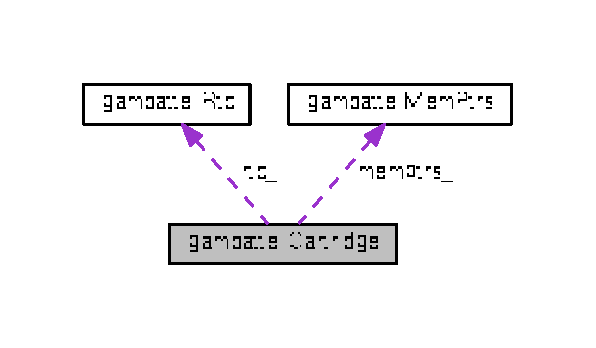
\includegraphics[width=286pt]{classgambatte_1_1Cartridge__coll__graph}
\end{center}
\end{figure}
\subsection*{Classes}
\begin{DoxyCompactItemize}
\item 
struct \hyperlink{structgambatte_1_1Cartridge_1_1AddrData}{Addr\+Data}
\end{DoxyCompactItemize}
\subsection*{Public Member Functions}
\begin{DoxyCompactItemize}
\item 
\hyperlink{classgambatte_1_1Cartridge_a02a7810564cf878e8a669b36818f760b}{Cartridge} (time\+\_\+t($\ast$$\ast$\+\_\+get\+Current\+Time)())
\item 
void \hyperlink{classgambatte_1_1Cartridge_ac4763db244cc009bfb86f169dec3f00a}{set\+State\+Ptrs} (\hyperlink{structgambatte_1_1SaveState}{Save\+State} \&)
\item 
void \hyperlink{classgambatte_1_1Cartridge_a0ac95a6edca7e01135de8808cb820850}{save\+State} (\hyperlink{structgambatte_1_1SaveState}{Save\+State} \&) const
\item 
void \hyperlink{classgambatte_1_1Cartridge_a2ea9929b798d88065ae39114a496d9b5}{load\+State} (\hyperlink{structgambatte_1_1SaveState}{Save\+State} const \&)
\item 
bool \hyperlink{classgambatte_1_1Cartridge_a765c0ba661feaa0f6ba9055a700f0cb4}{loaded} () const
\item 
\hyperlink{namespacegambatte_a2c5520a5fadf732ba8907450d802f51b}{Oam\+Dma\+Src} \hyperlink{classgambatte_1_1Cartridge_a32f9d2af10d44c526005df6c15f56e18}{oam\+Dma\+Src} () const
\item 
void \hyperlink{classgambatte_1_1Cartridge_a7a5643c7ff2f150fa67cf0570dfd06fa}{set\+Vrambank} (unsigned bank)
\item 
void \hyperlink{classgambatte_1_1Cartridge_a0b048b7d2c8eabdc557d1b4b80074345}{set\+Wrambank} (unsigned bank)
\item 
void \hyperlink{classgambatte_1_1Cartridge_a99aa834320ba188ae56edbd921aa99b6}{set\+Oam\+Dma\+Src} (\hyperlink{namespacegambatte_a2c5520a5fadf732ba8907450d802f51b}{Oam\+Dma\+Src} \hyperlink{classgambatte_1_1Cartridge_a32f9d2af10d44c526005df6c15f56e18}{oam\+Dma\+Src})
\item 
void \hyperlink{classgambatte_1_1Cartridge_ac560daf65ec58dfaee2b0142a2bc54af}{mbc\+Write} (unsigned addr, unsigned data)
\item 
bool \hyperlink{classgambatte_1_1Cartridge_a821a86fbca32b119dc3d18f99ff9ca42}{is\+Cgb} () const
\item 
void \hyperlink{classgambatte_1_1Cartridge_a0caa4fb15d1059ef3946988e581e526d}{rtc\+Write} (unsigned data)
\item 
unsigned char \hyperlink{classgambatte_1_1Cartridge_aa0c2605ee066351363516580e6945b16}{rtc\+Read} () const
\item 
void \hyperlink{classgambatte_1_1Cartridge_af46947d940c5b4ad32713c8c1070ae0e}{load\+Savedata} ()
\item 
void \hyperlink{classgambatte_1_1Cartridge_ae0d6195f96b7f3f986f96cedf97d79d3}{save\+Savedata} ()
\item 
std\+::string const \hyperlink{classgambatte_1_1Cartridge_a6943565180defed66c2c9242a95c2dd7}{save\+Base\+Path} () const
\item 
void \hyperlink{classgambatte_1_1Cartridge_ab2914efc5883a73590b0583f5aced2bf}{set\+Save\+Dir} (std\+::string const \&dir)
\item 
char const  $\ast$ \hyperlink{classgambatte_1_1Cartridge_a100de2429832931680f0b01439f118bc}{rom\+Title} () const
\item 
class \hyperlink{classgambatte_1_1PakInfo}{Pak\+Info} const \hyperlink{classgambatte_1_1Cartridge_aea12a1156e0af20786acca153daeea54}{pak\+Info} (bool multicart\+Compat) const
\item 
void \hyperlink{classgambatte_1_1Cartridge_aad77586072a86778761a52956600d8fa}{set\+Game\+Genie} (std\+::string const \&codes)
\item 
const unsigned char $\ast$ \hyperlink{classgambatte_1_1Cartridge_ade314f8bbf398736280ed18cc814295a}{rmem} (unsigned area) const
\item 
unsigned char $\ast$ \hyperlink{classgambatte_1_1Cartridge_ad52d62c1d71ed5dad84df200f2efe66f}{wmem} (unsigned area) const
\item 
unsigned char $\ast$ \hyperlink{classgambatte_1_1Cartridge_a24ebcceeda4d42ea537439cb2a038229}{vramdata} () const
\item 
unsigned char $\ast$ \hyperlink{classgambatte_1_1Cartridge_af1d0d66e9bf7fe8381d1ebea9838fcec}{romdata} (unsigned area) const
\item 
unsigned char $\ast$ \hyperlink{classgambatte_1_1Cartridge_a5e07be9371925ec3d5868bd3202bf539}{wramdata} (unsigned area) const
\item 
const unsigned char $\ast$ \hyperlink{classgambatte_1_1Cartridge_a9dbf0b52e895c34bb0e4fcce84fecf8f}{rdisabled\+Ram} () const
\item 
const unsigned char $\ast$ \hyperlink{classgambatte_1_1Cartridge_a42f315a3a5348cda032478e0c7ccb817}{rsrambankptr} () const
\item 
unsigned char $\ast$ \hyperlink{classgambatte_1_1Cartridge_a0c3fb4126497653f8b892bd41c52f641}{wsrambankptr} () const
\item 
unsigned char $\ast$ \hyperlink{classgambatte_1_1Cartridge_a96a47d8eabc979ebad658ad97ac1bbd2}{vrambankptr} () const
\item 
void \hyperlink{classgambatte_1_1Cartridge_a6030d5fcf47a55c793386b7f14ef9e1b}{load\+Or\+Save} (\hyperlink{classgambatte_1_1loadsave}{loadsave} \&\hyperlink{ppu_8cpp_a2f2eca6997ee7baf8901725ae074d45b}{state})
\item 
void \hyperlink{classgambatte_1_1Cartridge_a18df767dc053951e04d90dac74b4d160}{set\+Rtc\+Base} (time\+\_\+t time)
\item 
time\+\_\+t \hyperlink{classgambatte_1_1Cartridge_a7152d82b610d87112c591c63bdf4229b}{get\+Rtc\+Base} ()
\item 
std\+::pair$<$ unsigned char $\ast$, size\+\_\+t $>$ \hyperlink{classgambatte_1_1Cartridge_ab4fe1c7d62303984822c255aabaca906}{get\+Cart\+Rom} ()
\item 
std\+::pair$<$ unsigned char $\ast$, size\+\_\+t $>$ \hyperlink{classgambatte_1_1Cartridge_a62bda3afbd74966cf076253ab5c10fd4}{get\+Work\+Ram} ()
\item 
std\+::pair$<$ unsigned char $\ast$, size\+\_\+t $>$ \hyperlink{classgambatte_1_1Cartridge_a142bfdee87ed28bfdce9a71340d551b5}{get\+Save\+Ram} ()
\item 
std\+::pair$<$ unsigned char $\ast$, size\+\_\+t $>$ \hyperlink{classgambatte_1_1Cartridge_a2a7d9c624b3f344292a2f198dd57e62d}{get\+Video\+Ram} ()
\item 
\hyperlink{namespacegambatte_a42606f494711d2e2870a5f5cdf69e468}{Load\+Res} \hyperlink{classgambatte_1_1Cartridge_a28bde5fa09184ce6376555d85773c18f}{load\+R\+OM} (const std\+::string \&romfile, bool force\+Dmg, bool multicart\+Compat)
\item 
\hyperlink{namespacegambatte_a42606f494711d2e2870a5f5cdf69e468}{Load\+Res} \hyperlink{classgambatte_1_1Cartridge_ae6da096ff5dbaf07d3af3d581819237f}{load\+R\+OM} (const unsigned char $\ast$image, size\+\_\+t isize, bool force\+Dmg, bool multicart\+Compat)
\item 
\hyperlink{namespacegambatte_a42606f494711d2e2870a5f5cdf69e468}{Load\+Res} \hyperlink{classgambatte_1_1Cartridge_a2e7d7b90840269e9cd4a0c195556f53f}{load\+R\+OM} (\hyperlink{classgambatte_1_1File}{File} $\ast$rom, const bool force\+Dmg, const bool multicart\+Compat, const std\+::string \&\hyperlink{ioapi_8h_a7a03a664b090ce5c848ecb31cb4a2fa8}{filename})
\item 
void \hyperlink{classgambatte_1_1Cartridge_a14b11de7681f428ffd03178998e76506}{clear\+Memory\+Saved\+Data} ()
\end{DoxyCompactItemize}
\subsection*{Private Member Functions}
\begin{DoxyCompactItemize}
\item 
void \hyperlink{classgambatte_1_1Cartridge_ae8e53af5a4d2faeca8342e62924ec2bc}{apply\+Game\+Genie} (std\+::string const \&code)
\end{DoxyCompactItemize}
\subsection*{Private Attributes}
\begin{DoxyCompactItemize}
\item 
\hyperlink{classgambatte_1_1MemPtrs}{Mem\+Ptrs} \hyperlink{classgambatte_1_1Cartridge_ae4e6c2c7556a809cb6719f73fe256643}{memptrs\+\_\+}
\item 
\hyperlink{classgambatte_1_1Rtc}{Rtc} \hyperlink{classgambatte_1_1Cartridge_a32947bf947f84c9f98c30a1b413e91e6}{rtc\+\_\+}
\item 
scoped\+\_\+ptr$<$ \hyperlink{classgambatte_1_1Mbc}{Mbc} $>$ \hyperlink{classgambatte_1_1Cartridge_a94785054569a9ea1df0d3c9cea074ef8}{mbc\+\_\+}
\item 
std\+::string \hyperlink{classgambatte_1_1Cartridge_af35601276a25e69bb84f54bc864daeed}{default\+Save\+Base\+Path\+\_\+}
\item 
std\+::string \hyperlink{classgambatte_1_1Cartridge_a06acb91d23c878135eb7e8aefcc6de5f}{save\+Dir\+\_\+}
\item 
std\+::vector$<$ \hyperlink{structgambatte_1_1Cartridge_1_1AddrData}{Addr\+Data} $>$ \hyperlink{classgambatte_1_1Cartridge_a13d6eb2e426588bcf1e34f3b83c1b219}{gg\+Undo\+List\+\_\+}
\item 
bool \hyperlink{classgambatte_1_1Cartridge_a47d15c2e350647b805b299c73513451b}{memory\+Cartridge}
\item 
time\+\_\+t \hyperlink{classgambatte_1_1Cartridge_a81cec8cae288cc425bd90ff556536630}{memory\+Cartridge\+Rtc\+Base}
\item 
std\+::vector$<$ unsigned char $>$ \hyperlink{classgambatte_1_1Cartridge_a78010ede72a9fd7d82b4817a98df67cc}{memory\+Cartridge\+Sram}
\end{DoxyCompactItemize}


\subsection{Constructor \& Destructor Documentation}
\mbox{\Hypertarget{classgambatte_1_1Cartridge_a02a7810564cf878e8a669b36818f760b}\label{classgambatte_1_1Cartridge_a02a7810564cf878e8a669b36818f760b}} 
\index{gambatte\+::\+Cartridge@{gambatte\+::\+Cartridge}!Cartridge@{Cartridge}}
\index{Cartridge@{Cartridge}!gambatte\+::\+Cartridge@{gambatte\+::\+Cartridge}}
\subsubsection{\texorpdfstring{Cartridge()}{Cartridge()}}
{\footnotesize\ttfamily gambatte\+::\+Cartridge\+::\+Cartridge (\begin{DoxyParamCaption}\item[{time\+\_\+t($\ast$$\ast$)()}]{\+\_\+get\+Current\+Time }\end{DoxyParamCaption})}



\subsection{Member Function Documentation}
\mbox{\Hypertarget{classgambatte_1_1Cartridge_ae8e53af5a4d2faeca8342e62924ec2bc}\label{classgambatte_1_1Cartridge_ae8e53af5a4d2faeca8342e62924ec2bc}} 
\index{gambatte\+::\+Cartridge@{gambatte\+::\+Cartridge}!apply\+Game\+Genie@{apply\+Game\+Genie}}
\index{apply\+Game\+Genie@{apply\+Game\+Genie}!gambatte\+::\+Cartridge@{gambatte\+::\+Cartridge}}
\subsubsection{\texorpdfstring{apply\+Game\+Genie()}{applyGameGenie()}}
{\footnotesize\ttfamily void gambatte\+::\+Cartridge\+::apply\+Game\+Genie (\begin{DoxyParamCaption}\item[{std\+::string const \&}]{code }\end{DoxyParamCaption})\hspace{0.3cm}{\ttfamily [private]}}

\mbox{\Hypertarget{classgambatte_1_1Cartridge_a14b11de7681f428ffd03178998e76506}\label{classgambatte_1_1Cartridge_a14b11de7681f428ffd03178998e76506}} 
\index{gambatte\+::\+Cartridge@{gambatte\+::\+Cartridge}!clear\+Memory\+Saved\+Data@{clear\+Memory\+Saved\+Data}}
\index{clear\+Memory\+Saved\+Data@{clear\+Memory\+Saved\+Data}!gambatte\+::\+Cartridge@{gambatte\+::\+Cartridge}}
\subsubsection{\texorpdfstring{clear\+Memory\+Saved\+Data()}{clearMemorySavedData()}}
{\footnotesize\ttfamily void gambatte\+::\+Cartridge\+::clear\+Memory\+Saved\+Data (\begin{DoxyParamCaption}{ }\end{DoxyParamCaption})}

\mbox{\Hypertarget{classgambatte_1_1Cartridge_ab4fe1c7d62303984822c255aabaca906}\label{classgambatte_1_1Cartridge_ab4fe1c7d62303984822c255aabaca906}} 
\index{gambatte\+::\+Cartridge@{gambatte\+::\+Cartridge}!get\+Cart\+Rom@{get\+Cart\+Rom}}
\index{get\+Cart\+Rom@{get\+Cart\+Rom}!gambatte\+::\+Cartridge@{gambatte\+::\+Cartridge}}
\subsubsection{\texorpdfstring{get\+Cart\+Rom()}{getCartRom()}}
{\footnotesize\ttfamily std\+::pair$<$ unsigned char $\ast$, size\+\_\+t $>$ gambatte\+::\+Cartridge\+::get\+Cart\+Rom (\begin{DoxyParamCaption}{ }\end{DoxyParamCaption})}

\mbox{\Hypertarget{classgambatte_1_1Cartridge_a7152d82b610d87112c591c63bdf4229b}\label{classgambatte_1_1Cartridge_a7152d82b610d87112c591c63bdf4229b}} 
\index{gambatte\+::\+Cartridge@{gambatte\+::\+Cartridge}!get\+Rtc\+Base@{get\+Rtc\+Base}}
\index{get\+Rtc\+Base@{get\+Rtc\+Base}!gambatte\+::\+Cartridge@{gambatte\+::\+Cartridge}}
\subsubsection{\texorpdfstring{get\+Rtc\+Base()}{getRtcBase()}}
{\footnotesize\ttfamily time\+\_\+t gambatte\+::\+Cartridge\+::get\+Rtc\+Base (\begin{DoxyParamCaption}{ }\end{DoxyParamCaption})\hspace{0.3cm}{\ttfamily [inline]}}

\mbox{\Hypertarget{classgambatte_1_1Cartridge_a142bfdee87ed28bfdce9a71340d551b5}\label{classgambatte_1_1Cartridge_a142bfdee87ed28bfdce9a71340d551b5}} 
\index{gambatte\+::\+Cartridge@{gambatte\+::\+Cartridge}!get\+Save\+Ram@{get\+Save\+Ram}}
\index{get\+Save\+Ram@{get\+Save\+Ram}!gambatte\+::\+Cartridge@{gambatte\+::\+Cartridge}}
\subsubsection{\texorpdfstring{get\+Save\+Ram()}{getSaveRam()}}
{\footnotesize\ttfamily std\+::pair$<$ unsigned char $\ast$, size\+\_\+t $>$ gambatte\+::\+Cartridge\+::get\+Save\+Ram (\begin{DoxyParamCaption}{ }\end{DoxyParamCaption})}

\mbox{\Hypertarget{classgambatte_1_1Cartridge_a2a7d9c624b3f344292a2f198dd57e62d}\label{classgambatte_1_1Cartridge_a2a7d9c624b3f344292a2f198dd57e62d}} 
\index{gambatte\+::\+Cartridge@{gambatte\+::\+Cartridge}!get\+Video\+Ram@{get\+Video\+Ram}}
\index{get\+Video\+Ram@{get\+Video\+Ram}!gambatte\+::\+Cartridge@{gambatte\+::\+Cartridge}}
\subsubsection{\texorpdfstring{get\+Video\+Ram()}{getVideoRam()}}
{\footnotesize\ttfamily std\+::pair$<$ unsigned char $\ast$, size\+\_\+t $>$ gambatte\+::\+Cartridge\+::get\+Video\+Ram (\begin{DoxyParamCaption}{ }\end{DoxyParamCaption})}

\mbox{\Hypertarget{classgambatte_1_1Cartridge_a62bda3afbd74966cf076253ab5c10fd4}\label{classgambatte_1_1Cartridge_a62bda3afbd74966cf076253ab5c10fd4}} 
\index{gambatte\+::\+Cartridge@{gambatte\+::\+Cartridge}!get\+Work\+Ram@{get\+Work\+Ram}}
\index{get\+Work\+Ram@{get\+Work\+Ram}!gambatte\+::\+Cartridge@{gambatte\+::\+Cartridge}}
\subsubsection{\texorpdfstring{get\+Work\+Ram()}{getWorkRam()}}
{\footnotesize\ttfamily std\+::pair$<$ unsigned char $\ast$, size\+\_\+t $>$ gambatte\+::\+Cartridge\+::get\+Work\+Ram (\begin{DoxyParamCaption}{ }\end{DoxyParamCaption})}

\mbox{\Hypertarget{classgambatte_1_1Cartridge_a821a86fbca32b119dc3d18f99ff9ca42}\label{classgambatte_1_1Cartridge_a821a86fbca32b119dc3d18f99ff9ca42}} 
\index{gambatte\+::\+Cartridge@{gambatte\+::\+Cartridge}!is\+Cgb@{is\+Cgb}}
\index{is\+Cgb@{is\+Cgb}!gambatte\+::\+Cartridge@{gambatte\+::\+Cartridge}}
\subsubsection{\texorpdfstring{is\+Cgb()}{isCgb()}}
{\footnotesize\ttfamily bool gambatte\+::\+Cartridge\+::is\+Cgb (\begin{DoxyParamCaption}{ }\end{DoxyParamCaption}) const\hspace{0.3cm}{\ttfamily [inline]}}

\mbox{\Hypertarget{classgambatte_1_1Cartridge_a765c0ba661feaa0f6ba9055a700f0cb4}\label{classgambatte_1_1Cartridge_a765c0ba661feaa0f6ba9055a700f0cb4}} 
\index{gambatte\+::\+Cartridge@{gambatte\+::\+Cartridge}!loaded@{loaded}}
\index{loaded@{loaded}!gambatte\+::\+Cartridge@{gambatte\+::\+Cartridge}}
\subsubsection{\texorpdfstring{loaded()}{loaded()}}
{\footnotesize\ttfamily bool gambatte\+::\+Cartridge\+::loaded (\begin{DoxyParamCaption}{ }\end{DoxyParamCaption}) const\hspace{0.3cm}{\ttfamily [inline]}}

\mbox{\Hypertarget{classgambatte_1_1Cartridge_a6030d5fcf47a55c793386b7f14ef9e1b}\label{classgambatte_1_1Cartridge_a6030d5fcf47a55c793386b7f14ef9e1b}} 
\index{gambatte\+::\+Cartridge@{gambatte\+::\+Cartridge}!load\+Or\+Save@{load\+Or\+Save}}
\index{load\+Or\+Save@{load\+Or\+Save}!gambatte\+::\+Cartridge@{gambatte\+::\+Cartridge}}
\subsubsection{\texorpdfstring{load\+Or\+Save()}{loadOrSave()}}
{\footnotesize\ttfamily void gambatte\+::\+Cartridge\+::load\+Or\+Save (\begin{DoxyParamCaption}\item[{\hyperlink{classgambatte_1_1loadsave}{loadsave} \&}]{state }\end{DoxyParamCaption})}

\mbox{\Hypertarget{classgambatte_1_1Cartridge_a28bde5fa09184ce6376555d85773c18f}\label{classgambatte_1_1Cartridge_a28bde5fa09184ce6376555d85773c18f}} 
\index{gambatte\+::\+Cartridge@{gambatte\+::\+Cartridge}!load\+R\+OM@{load\+R\+OM}}
\index{load\+R\+OM@{load\+R\+OM}!gambatte\+::\+Cartridge@{gambatte\+::\+Cartridge}}
\subsubsection{\texorpdfstring{load\+R\+O\+M()}{loadROM()}\hspace{0.1cm}{\footnotesize\ttfamily [1/3]}}
{\footnotesize\ttfamily \hyperlink{namespacegambatte_a42606f494711d2e2870a5f5cdf69e468}{Load\+Res} gambatte\+::\+Cartridge\+::load\+R\+OM (\begin{DoxyParamCaption}\item[{const std\+::string \&}]{romfile,  }\item[{bool}]{force\+Dmg,  }\item[{bool}]{multicart\+Compat }\end{DoxyParamCaption})}

\mbox{\Hypertarget{classgambatte_1_1Cartridge_ae6da096ff5dbaf07d3af3d581819237f}\label{classgambatte_1_1Cartridge_ae6da096ff5dbaf07d3af3d581819237f}} 
\index{gambatte\+::\+Cartridge@{gambatte\+::\+Cartridge}!load\+R\+OM@{load\+R\+OM}}
\index{load\+R\+OM@{load\+R\+OM}!gambatte\+::\+Cartridge@{gambatte\+::\+Cartridge}}
\subsubsection{\texorpdfstring{load\+R\+O\+M()}{loadROM()}\hspace{0.1cm}{\footnotesize\ttfamily [2/3]}}
{\footnotesize\ttfamily \hyperlink{namespacegambatte_a42606f494711d2e2870a5f5cdf69e468}{Load\+Res} gambatte\+::\+Cartridge\+::load\+R\+OM (\begin{DoxyParamCaption}\item[{const unsigned char $\ast$}]{image,  }\item[{size\+\_\+t}]{isize,  }\item[{bool}]{force\+Dmg,  }\item[{bool}]{multicart\+Compat }\end{DoxyParamCaption})}

\mbox{\Hypertarget{classgambatte_1_1Cartridge_a2e7d7b90840269e9cd4a0c195556f53f}\label{classgambatte_1_1Cartridge_a2e7d7b90840269e9cd4a0c195556f53f}} 
\index{gambatte\+::\+Cartridge@{gambatte\+::\+Cartridge}!load\+R\+OM@{load\+R\+OM}}
\index{load\+R\+OM@{load\+R\+OM}!gambatte\+::\+Cartridge@{gambatte\+::\+Cartridge}}
\subsubsection{\texorpdfstring{load\+R\+O\+M()}{loadROM()}\hspace{0.1cm}{\footnotesize\ttfamily [3/3]}}
{\footnotesize\ttfamily \hyperlink{namespacegambatte_a42606f494711d2e2870a5f5cdf69e468}{Load\+Res} gambatte\+::\+Cartridge\+::load\+R\+OM (\begin{DoxyParamCaption}\item[{\hyperlink{classgambatte_1_1File}{File} $\ast$}]{rom,  }\item[{const bool}]{force\+Dmg,  }\item[{const bool}]{multicart\+Compat,  }\item[{const std\+::string \&}]{filename }\end{DoxyParamCaption})}

\mbox{\Hypertarget{classgambatte_1_1Cartridge_af46947d940c5b4ad32713c8c1070ae0e}\label{classgambatte_1_1Cartridge_af46947d940c5b4ad32713c8c1070ae0e}} 
\index{gambatte\+::\+Cartridge@{gambatte\+::\+Cartridge}!load\+Savedata@{load\+Savedata}}
\index{load\+Savedata@{load\+Savedata}!gambatte\+::\+Cartridge@{gambatte\+::\+Cartridge}}
\subsubsection{\texorpdfstring{load\+Savedata()}{loadSavedata()}}
{\footnotesize\ttfamily void gambatte\+::\+Cartridge\+::load\+Savedata (\begin{DoxyParamCaption}{ }\end{DoxyParamCaption})}

\mbox{\Hypertarget{classgambatte_1_1Cartridge_a2ea9929b798d88065ae39114a496d9b5}\label{classgambatte_1_1Cartridge_a2ea9929b798d88065ae39114a496d9b5}} 
\index{gambatte\+::\+Cartridge@{gambatte\+::\+Cartridge}!load\+State@{load\+State}}
\index{load\+State@{load\+State}!gambatte\+::\+Cartridge@{gambatte\+::\+Cartridge}}
\subsubsection{\texorpdfstring{load\+State()}{loadState()}}
{\footnotesize\ttfamily void gambatte\+::\+Cartridge\+::load\+State (\begin{DoxyParamCaption}\item[{\hyperlink{structgambatte_1_1SaveState}{Save\+State} const \&}]{state }\end{DoxyParamCaption})}

\mbox{\Hypertarget{classgambatte_1_1Cartridge_ac560daf65ec58dfaee2b0142a2bc54af}\label{classgambatte_1_1Cartridge_ac560daf65ec58dfaee2b0142a2bc54af}} 
\index{gambatte\+::\+Cartridge@{gambatte\+::\+Cartridge}!mbc\+Write@{mbc\+Write}}
\index{mbc\+Write@{mbc\+Write}!gambatte\+::\+Cartridge@{gambatte\+::\+Cartridge}}
\subsubsection{\texorpdfstring{mbc\+Write()}{mbcWrite()}}
{\footnotesize\ttfamily void gambatte\+::\+Cartridge\+::mbc\+Write (\begin{DoxyParamCaption}\item[{unsigned}]{addr,  }\item[{unsigned}]{data }\end{DoxyParamCaption})\hspace{0.3cm}{\ttfamily [inline]}}

\mbox{\Hypertarget{classgambatte_1_1Cartridge_a32f9d2af10d44c526005df6c15f56e18}\label{classgambatte_1_1Cartridge_a32f9d2af10d44c526005df6c15f56e18}} 
\index{gambatte\+::\+Cartridge@{gambatte\+::\+Cartridge}!oam\+Dma\+Src@{oam\+Dma\+Src}}
\index{oam\+Dma\+Src@{oam\+Dma\+Src}!gambatte\+::\+Cartridge@{gambatte\+::\+Cartridge}}
\subsubsection{\texorpdfstring{oam\+Dma\+Src()}{oamDmaSrc()}}
{\footnotesize\ttfamily \hyperlink{namespacegambatte_a2c5520a5fadf732ba8907450d802f51b}{Oam\+Dma\+Src} gambatte\+::\+Cartridge\+::oam\+Dma\+Src (\begin{DoxyParamCaption}{ }\end{DoxyParamCaption}) const\hspace{0.3cm}{\ttfamily [inline]}}

\mbox{\Hypertarget{classgambatte_1_1Cartridge_aea12a1156e0af20786acca153daeea54}\label{classgambatte_1_1Cartridge_aea12a1156e0af20786acca153daeea54}} 
\index{gambatte\+::\+Cartridge@{gambatte\+::\+Cartridge}!pak\+Info@{pak\+Info}}
\index{pak\+Info@{pak\+Info}!gambatte\+::\+Cartridge@{gambatte\+::\+Cartridge}}
\subsubsection{\texorpdfstring{pak\+Info()}{pakInfo()}}
{\footnotesize\ttfamily \hyperlink{classgambatte_1_1PakInfo}{Pak\+Info} const gambatte\+::\+Cartridge\+::pak\+Info (\begin{DoxyParamCaption}\item[{bool}]{multicart\+Compat }\end{DoxyParamCaption}) const}

\mbox{\Hypertarget{classgambatte_1_1Cartridge_a9dbf0b52e895c34bb0e4fcce84fecf8f}\label{classgambatte_1_1Cartridge_a9dbf0b52e895c34bb0e4fcce84fecf8f}} 
\index{gambatte\+::\+Cartridge@{gambatte\+::\+Cartridge}!rdisabled\+Ram@{rdisabled\+Ram}}
\index{rdisabled\+Ram@{rdisabled\+Ram}!gambatte\+::\+Cartridge@{gambatte\+::\+Cartridge}}
\subsubsection{\texorpdfstring{rdisabled\+Ram()}{rdisabledRam()}}
{\footnotesize\ttfamily const unsigned char$\ast$ gambatte\+::\+Cartridge\+::rdisabled\+Ram (\begin{DoxyParamCaption}{ }\end{DoxyParamCaption}) const\hspace{0.3cm}{\ttfamily [inline]}}

\mbox{\Hypertarget{classgambatte_1_1Cartridge_ade314f8bbf398736280ed18cc814295a}\label{classgambatte_1_1Cartridge_ade314f8bbf398736280ed18cc814295a}} 
\index{gambatte\+::\+Cartridge@{gambatte\+::\+Cartridge}!rmem@{rmem}}
\index{rmem@{rmem}!gambatte\+::\+Cartridge@{gambatte\+::\+Cartridge}}
\subsubsection{\texorpdfstring{rmem()}{rmem()}}
{\footnotesize\ttfamily const unsigned char$\ast$ gambatte\+::\+Cartridge\+::rmem (\begin{DoxyParamCaption}\item[{unsigned}]{area }\end{DoxyParamCaption}) const\hspace{0.3cm}{\ttfamily [inline]}}

\mbox{\Hypertarget{classgambatte_1_1Cartridge_af1d0d66e9bf7fe8381d1ebea9838fcec}\label{classgambatte_1_1Cartridge_af1d0d66e9bf7fe8381d1ebea9838fcec}} 
\index{gambatte\+::\+Cartridge@{gambatte\+::\+Cartridge}!romdata@{romdata}}
\index{romdata@{romdata}!gambatte\+::\+Cartridge@{gambatte\+::\+Cartridge}}
\subsubsection{\texorpdfstring{romdata()}{romdata()}}
{\footnotesize\ttfamily unsigned char$\ast$ gambatte\+::\+Cartridge\+::romdata (\begin{DoxyParamCaption}\item[{unsigned}]{area }\end{DoxyParamCaption}) const\hspace{0.3cm}{\ttfamily [inline]}}

\mbox{\Hypertarget{classgambatte_1_1Cartridge_a100de2429832931680f0b01439f118bc}\label{classgambatte_1_1Cartridge_a100de2429832931680f0b01439f118bc}} 
\index{gambatte\+::\+Cartridge@{gambatte\+::\+Cartridge}!rom\+Title@{rom\+Title}}
\index{rom\+Title@{rom\+Title}!gambatte\+::\+Cartridge@{gambatte\+::\+Cartridge}}
\subsubsection{\texorpdfstring{rom\+Title()}{romTitle()}}
{\footnotesize\ttfamily char const$\ast$ gambatte\+::\+Cartridge\+::rom\+Title (\begin{DoxyParamCaption}{ }\end{DoxyParamCaption}) const\hspace{0.3cm}{\ttfamily [inline]}}

\mbox{\Hypertarget{classgambatte_1_1Cartridge_a42f315a3a5348cda032478e0c7ccb817}\label{classgambatte_1_1Cartridge_a42f315a3a5348cda032478e0c7ccb817}} 
\index{gambatte\+::\+Cartridge@{gambatte\+::\+Cartridge}!rsrambankptr@{rsrambankptr}}
\index{rsrambankptr@{rsrambankptr}!gambatte\+::\+Cartridge@{gambatte\+::\+Cartridge}}
\subsubsection{\texorpdfstring{rsrambankptr()}{rsrambankptr()}}
{\footnotesize\ttfamily const unsigned char$\ast$ gambatte\+::\+Cartridge\+::rsrambankptr (\begin{DoxyParamCaption}{ }\end{DoxyParamCaption}) const\hspace{0.3cm}{\ttfamily [inline]}}

\mbox{\Hypertarget{classgambatte_1_1Cartridge_aa0c2605ee066351363516580e6945b16}\label{classgambatte_1_1Cartridge_aa0c2605ee066351363516580e6945b16}} 
\index{gambatte\+::\+Cartridge@{gambatte\+::\+Cartridge}!rtc\+Read@{rtc\+Read}}
\index{rtc\+Read@{rtc\+Read}!gambatte\+::\+Cartridge@{gambatte\+::\+Cartridge}}
\subsubsection{\texorpdfstring{rtc\+Read()}{rtcRead()}}
{\footnotesize\ttfamily unsigned char gambatte\+::\+Cartridge\+::rtc\+Read (\begin{DoxyParamCaption}{ }\end{DoxyParamCaption}) const\hspace{0.3cm}{\ttfamily [inline]}}

\mbox{\Hypertarget{classgambatte_1_1Cartridge_a0caa4fb15d1059ef3946988e581e526d}\label{classgambatte_1_1Cartridge_a0caa4fb15d1059ef3946988e581e526d}} 
\index{gambatte\+::\+Cartridge@{gambatte\+::\+Cartridge}!rtc\+Write@{rtc\+Write}}
\index{rtc\+Write@{rtc\+Write}!gambatte\+::\+Cartridge@{gambatte\+::\+Cartridge}}
\subsubsection{\texorpdfstring{rtc\+Write()}{rtcWrite()}}
{\footnotesize\ttfamily void gambatte\+::\+Cartridge\+::rtc\+Write (\begin{DoxyParamCaption}\item[{unsigned}]{data }\end{DoxyParamCaption})\hspace{0.3cm}{\ttfamily [inline]}}

\mbox{\Hypertarget{classgambatte_1_1Cartridge_a6943565180defed66c2c9242a95c2dd7}\label{classgambatte_1_1Cartridge_a6943565180defed66c2c9242a95c2dd7}} 
\index{gambatte\+::\+Cartridge@{gambatte\+::\+Cartridge}!save\+Base\+Path@{save\+Base\+Path}}
\index{save\+Base\+Path@{save\+Base\+Path}!gambatte\+::\+Cartridge@{gambatte\+::\+Cartridge}}
\subsubsection{\texorpdfstring{save\+Base\+Path()}{saveBasePath()}}
{\footnotesize\ttfamily std\+::string const gambatte\+::\+Cartridge\+::save\+Base\+Path (\begin{DoxyParamCaption}{ }\end{DoxyParamCaption}) const}

\mbox{\Hypertarget{classgambatte_1_1Cartridge_ae0d6195f96b7f3f986f96cedf97d79d3}\label{classgambatte_1_1Cartridge_ae0d6195f96b7f3f986f96cedf97d79d3}} 
\index{gambatte\+::\+Cartridge@{gambatte\+::\+Cartridge}!save\+Savedata@{save\+Savedata}}
\index{save\+Savedata@{save\+Savedata}!gambatte\+::\+Cartridge@{gambatte\+::\+Cartridge}}
\subsubsection{\texorpdfstring{save\+Savedata()}{saveSavedata()}}
{\footnotesize\ttfamily void gambatte\+::\+Cartridge\+::save\+Savedata (\begin{DoxyParamCaption}{ }\end{DoxyParamCaption})}

\mbox{\Hypertarget{classgambatte_1_1Cartridge_a0ac95a6edca7e01135de8808cb820850}\label{classgambatte_1_1Cartridge_a0ac95a6edca7e01135de8808cb820850}} 
\index{gambatte\+::\+Cartridge@{gambatte\+::\+Cartridge}!save\+State@{save\+State}}
\index{save\+State@{save\+State}!gambatte\+::\+Cartridge@{gambatte\+::\+Cartridge}}
\subsubsection{\texorpdfstring{save\+State()}{saveState()}}
{\footnotesize\ttfamily void gambatte\+::\+Cartridge\+::save\+State (\begin{DoxyParamCaption}\item[{\hyperlink{structgambatte_1_1SaveState}{Save\+State} \&}]{state }\end{DoxyParamCaption}) const}

\mbox{\Hypertarget{classgambatte_1_1Cartridge_aad77586072a86778761a52956600d8fa}\label{classgambatte_1_1Cartridge_aad77586072a86778761a52956600d8fa}} 
\index{gambatte\+::\+Cartridge@{gambatte\+::\+Cartridge}!set\+Game\+Genie@{set\+Game\+Genie}}
\index{set\+Game\+Genie@{set\+Game\+Genie}!gambatte\+::\+Cartridge@{gambatte\+::\+Cartridge}}
\subsubsection{\texorpdfstring{set\+Game\+Genie()}{setGameGenie()}}
{\footnotesize\ttfamily void gambatte\+::\+Cartridge\+::set\+Game\+Genie (\begin{DoxyParamCaption}\item[{std\+::string const \&}]{codes }\end{DoxyParamCaption})}

\mbox{\Hypertarget{classgambatte_1_1Cartridge_a99aa834320ba188ae56edbd921aa99b6}\label{classgambatte_1_1Cartridge_a99aa834320ba188ae56edbd921aa99b6}} 
\index{gambatte\+::\+Cartridge@{gambatte\+::\+Cartridge}!set\+Oam\+Dma\+Src@{set\+Oam\+Dma\+Src}}
\index{set\+Oam\+Dma\+Src@{set\+Oam\+Dma\+Src}!gambatte\+::\+Cartridge@{gambatte\+::\+Cartridge}}
\subsubsection{\texorpdfstring{set\+Oam\+Dma\+Src()}{setOamDmaSrc()}}
{\footnotesize\ttfamily void gambatte\+::\+Cartridge\+::set\+Oam\+Dma\+Src (\begin{DoxyParamCaption}\item[{\hyperlink{namespacegambatte_a2c5520a5fadf732ba8907450d802f51b}{Oam\+Dma\+Src}}]{oam\+Dma\+Src }\end{DoxyParamCaption})\hspace{0.3cm}{\ttfamily [inline]}}

\mbox{\Hypertarget{classgambatte_1_1Cartridge_a18df767dc053951e04d90dac74b4d160}\label{classgambatte_1_1Cartridge_a18df767dc053951e04d90dac74b4d160}} 
\index{gambatte\+::\+Cartridge@{gambatte\+::\+Cartridge}!set\+Rtc\+Base@{set\+Rtc\+Base}}
\index{set\+Rtc\+Base@{set\+Rtc\+Base}!gambatte\+::\+Cartridge@{gambatte\+::\+Cartridge}}
\subsubsection{\texorpdfstring{set\+Rtc\+Base()}{setRtcBase()}}
{\footnotesize\ttfamily void gambatte\+::\+Cartridge\+::set\+Rtc\+Base (\begin{DoxyParamCaption}\item[{time\+\_\+t}]{time }\end{DoxyParamCaption})\hspace{0.3cm}{\ttfamily [inline]}}

\mbox{\Hypertarget{classgambatte_1_1Cartridge_ab2914efc5883a73590b0583f5aced2bf}\label{classgambatte_1_1Cartridge_ab2914efc5883a73590b0583f5aced2bf}} 
\index{gambatte\+::\+Cartridge@{gambatte\+::\+Cartridge}!set\+Save\+Dir@{set\+Save\+Dir}}
\index{set\+Save\+Dir@{set\+Save\+Dir}!gambatte\+::\+Cartridge@{gambatte\+::\+Cartridge}}
\subsubsection{\texorpdfstring{set\+Save\+Dir()}{setSaveDir()}}
{\footnotesize\ttfamily void gambatte\+::\+Cartridge\+::set\+Save\+Dir (\begin{DoxyParamCaption}\item[{std\+::string const \&}]{dir }\end{DoxyParamCaption})}

\mbox{\Hypertarget{classgambatte_1_1Cartridge_ac4763db244cc009bfb86f169dec3f00a}\label{classgambatte_1_1Cartridge_ac4763db244cc009bfb86f169dec3f00a}} 
\index{gambatte\+::\+Cartridge@{gambatte\+::\+Cartridge}!set\+State\+Ptrs@{set\+State\+Ptrs}}
\index{set\+State\+Ptrs@{set\+State\+Ptrs}!gambatte\+::\+Cartridge@{gambatte\+::\+Cartridge}}
\subsubsection{\texorpdfstring{set\+State\+Ptrs()}{setStatePtrs()}}
{\footnotesize\ttfamily void gambatte\+::\+Cartridge\+::set\+State\+Ptrs (\begin{DoxyParamCaption}\item[{\hyperlink{structgambatte_1_1SaveState}{Save\+State} \&}]{state }\end{DoxyParamCaption})}

\mbox{\Hypertarget{classgambatte_1_1Cartridge_a7a5643c7ff2f150fa67cf0570dfd06fa}\label{classgambatte_1_1Cartridge_a7a5643c7ff2f150fa67cf0570dfd06fa}} 
\index{gambatte\+::\+Cartridge@{gambatte\+::\+Cartridge}!set\+Vrambank@{set\+Vrambank}}
\index{set\+Vrambank@{set\+Vrambank}!gambatte\+::\+Cartridge@{gambatte\+::\+Cartridge}}
\subsubsection{\texorpdfstring{set\+Vrambank()}{setVrambank()}}
{\footnotesize\ttfamily void gambatte\+::\+Cartridge\+::set\+Vrambank (\begin{DoxyParamCaption}\item[{unsigned}]{bank }\end{DoxyParamCaption})\hspace{0.3cm}{\ttfamily [inline]}}

\mbox{\Hypertarget{classgambatte_1_1Cartridge_a0b048b7d2c8eabdc557d1b4b80074345}\label{classgambatte_1_1Cartridge_a0b048b7d2c8eabdc557d1b4b80074345}} 
\index{gambatte\+::\+Cartridge@{gambatte\+::\+Cartridge}!set\+Wrambank@{set\+Wrambank}}
\index{set\+Wrambank@{set\+Wrambank}!gambatte\+::\+Cartridge@{gambatte\+::\+Cartridge}}
\subsubsection{\texorpdfstring{set\+Wrambank()}{setWrambank()}}
{\footnotesize\ttfamily void gambatte\+::\+Cartridge\+::set\+Wrambank (\begin{DoxyParamCaption}\item[{unsigned}]{bank }\end{DoxyParamCaption})\hspace{0.3cm}{\ttfamily [inline]}}

\mbox{\Hypertarget{classgambatte_1_1Cartridge_a96a47d8eabc979ebad658ad97ac1bbd2}\label{classgambatte_1_1Cartridge_a96a47d8eabc979ebad658ad97ac1bbd2}} 
\index{gambatte\+::\+Cartridge@{gambatte\+::\+Cartridge}!vrambankptr@{vrambankptr}}
\index{vrambankptr@{vrambankptr}!gambatte\+::\+Cartridge@{gambatte\+::\+Cartridge}}
\subsubsection{\texorpdfstring{vrambankptr()}{vrambankptr()}}
{\footnotesize\ttfamily unsigned char$\ast$ gambatte\+::\+Cartridge\+::vrambankptr (\begin{DoxyParamCaption}{ }\end{DoxyParamCaption}) const\hspace{0.3cm}{\ttfamily [inline]}}

\mbox{\Hypertarget{classgambatte_1_1Cartridge_a24ebcceeda4d42ea537439cb2a038229}\label{classgambatte_1_1Cartridge_a24ebcceeda4d42ea537439cb2a038229}} 
\index{gambatte\+::\+Cartridge@{gambatte\+::\+Cartridge}!vramdata@{vramdata}}
\index{vramdata@{vramdata}!gambatte\+::\+Cartridge@{gambatte\+::\+Cartridge}}
\subsubsection{\texorpdfstring{vramdata()}{vramdata()}}
{\footnotesize\ttfamily unsigned char$\ast$ gambatte\+::\+Cartridge\+::vramdata (\begin{DoxyParamCaption}{ }\end{DoxyParamCaption}) const\hspace{0.3cm}{\ttfamily [inline]}}

\mbox{\Hypertarget{classgambatte_1_1Cartridge_ad52d62c1d71ed5dad84df200f2efe66f}\label{classgambatte_1_1Cartridge_ad52d62c1d71ed5dad84df200f2efe66f}} 
\index{gambatte\+::\+Cartridge@{gambatte\+::\+Cartridge}!wmem@{wmem}}
\index{wmem@{wmem}!gambatte\+::\+Cartridge@{gambatte\+::\+Cartridge}}
\subsubsection{\texorpdfstring{wmem()}{wmem()}}
{\footnotesize\ttfamily unsigned char$\ast$ gambatte\+::\+Cartridge\+::wmem (\begin{DoxyParamCaption}\item[{unsigned}]{area }\end{DoxyParamCaption}) const\hspace{0.3cm}{\ttfamily [inline]}}

\mbox{\Hypertarget{classgambatte_1_1Cartridge_a5e07be9371925ec3d5868bd3202bf539}\label{classgambatte_1_1Cartridge_a5e07be9371925ec3d5868bd3202bf539}} 
\index{gambatte\+::\+Cartridge@{gambatte\+::\+Cartridge}!wramdata@{wramdata}}
\index{wramdata@{wramdata}!gambatte\+::\+Cartridge@{gambatte\+::\+Cartridge}}
\subsubsection{\texorpdfstring{wramdata()}{wramdata()}}
{\footnotesize\ttfamily unsigned char$\ast$ gambatte\+::\+Cartridge\+::wramdata (\begin{DoxyParamCaption}\item[{unsigned}]{area }\end{DoxyParamCaption}) const\hspace{0.3cm}{\ttfamily [inline]}}

\mbox{\Hypertarget{classgambatte_1_1Cartridge_a0c3fb4126497653f8b892bd41c52f641}\label{classgambatte_1_1Cartridge_a0c3fb4126497653f8b892bd41c52f641}} 
\index{gambatte\+::\+Cartridge@{gambatte\+::\+Cartridge}!wsrambankptr@{wsrambankptr}}
\index{wsrambankptr@{wsrambankptr}!gambatte\+::\+Cartridge@{gambatte\+::\+Cartridge}}
\subsubsection{\texorpdfstring{wsrambankptr()}{wsrambankptr()}}
{\footnotesize\ttfamily unsigned char$\ast$ gambatte\+::\+Cartridge\+::wsrambankptr (\begin{DoxyParamCaption}{ }\end{DoxyParamCaption}) const\hspace{0.3cm}{\ttfamily [inline]}}



\subsection{Member Data Documentation}
\mbox{\Hypertarget{classgambatte_1_1Cartridge_af35601276a25e69bb84f54bc864daeed}\label{classgambatte_1_1Cartridge_af35601276a25e69bb84f54bc864daeed}} 
\index{gambatte\+::\+Cartridge@{gambatte\+::\+Cartridge}!default\+Save\+Base\+Path\+\_\+@{default\+Save\+Base\+Path\+\_\+}}
\index{default\+Save\+Base\+Path\+\_\+@{default\+Save\+Base\+Path\+\_\+}!gambatte\+::\+Cartridge@{gambatte\+::\+Cartridge}}
\subsubsection{\texorpdfstring{default\+Save\+Base\+Path\+\_\+}{defaultSaveBasePath\_}}
{\footnotesize\ttfamily std\+::string gambatte\+::\+Cartridge\+::default\+Save\+Base\+Path\+\_\+\hspace{0.3cm}{\ttfamily [private]}}

\mbox{\Hypertarget{classgambatte_1_1Cartridge_a13d6eb2e426588bcf1e34f3b83c1b219}\label{classgambatte_1_1Cartridge_a13d6eb2e426588bcf1e34f3b83c1b219}} 
\index{gambatte\+::\+Cartridge@{gambatte\+::\+Cartridge}!gg\+Undo\+List\+\_\+@{gg\+Undo\+List\+\_\+}}
\index{gg\+Undo\+List\+\_\+@{gg\+Undo\+List\+\_\+}!gambatte\+::\+Cartridge@{gambatte\+::\+Cartridge}}
\subsubsection{\texorpdfstring{gg\+Undo\+List\+\_\+}{ggUndoList\_}}
{\footnotesize\ttfamily std\+::vector$<$\hyperlink{structgambatte_1_1Cartridge_1_1AddrData}{Addr\+Data}$>$ gambatte\+::\+Cartridge\+::gg\+Undo\+List\+\_\+\hspace{0.3cm}{\ttfamily [private]}}

\mbox{\Hypertarget{classgambatte_1_1Cartridge_a94785054569a9ea1df0d3c9cea074ef8}\label{classgambatte_1_1Cartridge_a94785054569a9ea1df0d3c9cea074ef8}} 
\index{gambatte\+::\+Cartridge@{gambatte\+::\+Cartridge}!mbc\+\_\+@{mbc\+\_\+}}
\index{mbc\+\_\+@{mbc\+\_\+}!gambatte\+::\+Cartridge@{gambatte\+::\+Cartridge}}
\subsubsection{\texorpdfstring{mbc\+\_\+}{mbc\_}}
{\footnotesize\ttfamily scoped\+\_\+ptr$<$\hyperlink{classgambatte_1_1Mbc}{Mbc}$>$ gambatte\+::\+Cartridge\+::mbc\+\_\+\hspace{0.3cm}{\ttfamily [private]}}

\mbox{\Hypertarget{classgambatte_1_1Cartridge_a47d15c2e350647b805b299c73513451b}\label{classgambatte_1_1Cartridge_a47d15c2e350647b805b299c73513451b}} 
\index{gambatte\+::\+Cartridge@{gambatte\+::\+Cartridge}!memory\+Cartridge@{memory\+Cartridge}}
\index{memory\+Cartridge@{memory\+Cartridge}!gambatte\+::\+Cartridge@{gambatte\+::\+Cartridge}}
\subsubsection{\texorpdfstring{memory\+Cartridge}{memoryCartridge}}
{\footnotesize\ttfamily bool gambatte\+::\+Cartridge\+::memory\+Cartridge\hspace{0.3cm}{\ttfamily [private]}}

\mbox{\Hypertarget{classgambatte_1_1Cartridge_a81cec8cae288cc425bd90ff556536630}\label{classgambatte_1_1Cartridge_a81cec8cae288cc425bd90ff556536630}} 
\index{gambatte\+::\+Cartridge@{gambatte\+::\+Cartridge}!memory\+Cartridge\+Rtc\+Base@{memory\+Cartridge\+Rtc\+Base}}
\index{memory\+Cartridge\+Rtc\+Base@{memory\+Cartridge\+Rtc\+Base}!gambatte\+::\+Cartridge@{gambatte\+::\+Cartridge}}
\subsubsection{\texorpdfstring{memory\+Cartridge\+Rtc\+Base}{memoryCartridgeRtcBase}}
{\footnotesize\ttfamily time\+\_\+t gambatte\+::\+Cartridge\+::memory\+Cartridge\+Rtc\+Base\hspace{0.3cm}{\ttfamily [private]}}

\mbox{\Hypertarget{classgambatte_1_1Cartridge_a78010ede72a9fd7d82b4817a98df67cc}\label{classgambatte_1_1Cartridge_a78010ede72a9fd7d82b4817a98df67cc}} 
\index{gambatte\+::\+Cartridge@{gambatte\+::\+Cartridge}!memory\+Cartridge\+Sram@{memory\+Cartridge\+Sram}}
\index{memory\+Cartridge\+Sram@{memory\+Cartridge\+Sram}!gambatte\+::\+Cartridge@{gambatte\+::\+Cartridge}}
\subsubsection{\texorpdfstring{memory\+Cartridge\+Sram}{memoryCartridgeSram}}
{\footnotesize\ttfamily std\+::vector$<$unsigned char$>$ gambatte\+::\+Cartridge\+::memory\+Cartridge\+Sram\hspace{0.3cm}{\ttfamily [private]}}

\mbox{\Hypertarget{classgambatte_1_1Cartridge_ae4e6c2c7556a809cb6719f73fe256643}\label{classgambatte_1_1Cartridge_ae4e6c2c7556a809cb6719f73fe256643}} 
\index{gambatte\+::\+Cartridge@{gambatte\+::\+Cartridge}!memptrs\+\_\+@{memptrs\+\_\+}}
\index{memptrs\+\_\+@{memptrs\+\_\+}!gambatte\+::\+Cartridge@{gambatte\+::\+Cartridge}}
\subsubsection{\texorpdfstring{memptrs\+\_\+}{memptrs\_}}
{\footnotesize\ttfamily \hyperlink{classgambatte_1_1MemPtrs}{Mem\+Ptrs} gambatte\+::\+Cartridge\+::memptrs\+\_\+\hspace{0.3cm}{\ttfamily [private]}}

\mbox{\Hypertarget{classgambatte_1_1Cartridge_a32947bf947f84c9f98c30a1b413e91e6}\label{classgambatte_1_1Cartridge_a32947bf947f84c9f98c30a1b413e91e6}} 
\index{gambatte\+::\+Cartridge@{gambatte\+::\+Cartridge}!rtc\+\_\+@{rtc\+\_\+}}
\index{rtc\+\_\+@{rtc\+\_\+}!gambatte\+::\+Cartridge@{gambatte\+::\+Cartridge}}
\subsubsection{\texorpdfstring{rtc\+\_\+}{rtc\_}}
{\footnotesize\ttfamily \hyperlink{classgambatte_1_1Rtc}{Rtc} gambatte\+::\+Cartridge\+::rtc\+\_\+\hspace{0.3cm}{\ttfamily [private]}}

\mbox{\Hypertarget{classgambatte_1_1Cartridge_a06acb91d23c878135eb7e8aefcc6de5f}\label{classgambatte_1_1Cartridge_a06acb91d23c878135eb7e8aefcc6de5f}} 
\index{gambatte\+::\+Cartridge@{gambatte\+::\+Cartridge}!save\+Dir\+\_\+@{save\+Dir\+\_\+}}
\index{save\+Dir\+\_\+@{save\+Dir\+\_\+}!gambatte\+::\+Cartridge@{gambatte\+::\+Cartridge}}
\subsubsection{\texorpdfstring{save\+Dir\+\_\+}{saveDir\_}}
{\footnotesize\ttfamily std\+::string gambatte\+::\+Cartridge\+::save\+Dir\+\_\+\hspace{0.3cm}{\ttfamily [private]}}



The documentation for this class was generated from the following files\+:\begin{DoxyCompactItemize}
\item 
src/mem/\hyperlink{cartridge_8h}{cartridge.\+h}\item 
src/mem/\hyperlink{cartridge_8cpp}{cartridge.\+cpp}\end{DoxyCompactItemize}

\hypertarget{structMinKeeperUtil_1_1CeiledLog2}{}\section{Min\+Keeper\+Util\+:\+:Ceiled\+Log2$<$ n $>$ Struct Template Reference}
\label{structMinKeeperUtil_1_1CeiledLog2}\index{Min\+Keeper\+Util\+::\+Ceiled\+Log2$<$ n $>$@{Min\+Keeper\+Util\+::\+Ceiled\+Log2$<$ n $>$}}


{\ttfamily \#include $<$minkeeper.\+h$>$}

\subsection*{Public Types}
\begin{DoxyCompactItemize}
\item 
enum \{ \hyperlink{structMinKeeperUtil_1_1CeiledLog2_ae163e7299724c7e999e7bdc0bf4f37e8a166207d435f94e516e36c590e9936e94}{r} = 1 + Ceiled\+Log2$<$(n + 1) / 2$>$\+:\+:r
 \}
\end{DoxyCompactItemize}


\subsection{Member Enumeration Documentation}
\mbox{\Hypertarget{structMinKeeperUtil_1_1CeiledLog2_ae163e7299724c7e999e7bdc0bf4f37e8}\label{structMinKeeperUtil_1_1CeiledLog2_ae163e7299724c7e999e7bdc0bf4f37e8}} 
\subsubsection{\texorpdfstring{anonymous enum}{anonymous enum}}
{\footnotesize\ttfamily template$<$int n$>$ \\
anonymous enum}

\begin{DoxyEnumFields}{Enumerator}
\raisebox{\heightof{T}}[0pt][0pt]{\index{r@{r}!Min\+Keeper\+Util\+::\+Ceiled\+Log2@{Min\+Keeper\+Util\+::\+Ceiled\+Log2}}\index{Min\+Keeper\+Util\+::\+Ceiled\+Log2@{Min\+Keeper\+Util\+::\+Ceiled\+Log2}!r@{r}}}\mbox{\Hypertarget{structMinKeeperUtil_1_1CeiledLog2_ae163e7299724c7e999e7bdc0bf4f37e8a166207d435f94e516e36c590e9936e94}\label{structMinKeeperUtil_1_1CeiledLog2_ae163e7299724c7e999e7bdc0bf4f37e8a166207d435f94e516e36c590e9936e94}} 
r&\\
\hline

\end{DoxyEnumFields}


The documentation for this struct was generated from the following file\+:\begin{DoxyCompactItemize}
\item 
src/\hyperlink{minkeeper_8h}{minkeeper.\+h}\end{DoxyCompactItemize}

\hypertarget{structMinKeeperUtil_1_1CeiledLog2_3_011_01_4}{}\section{Min\+Keeper\+Util\+:\+:Ceiled\+Log2$<$ 1 $>$ Struct Template Reference}
\label{structMinKeeperUtil_1_1CeiledLog2_3_011_01_4}\index{Min\+Keeper\+Util\+::\+Ceiled\+Log2$<$ 1 $>$@{Min\+Keeper\+Util\+::\+Ceiled\+Log2$<$ 1 $>$}}


{\ttfamily \#include $<$minkeeper.\+h$>$}

\subsection*{Public Types}
\begin{DoxyCompactItemize}
\item 
enum \{ \hyperlink{structMinKeeperUtil_1_1CeiledLog2_3_011_01_4_aa5d5d5cc1108d764e0f2ac3dcea396b9a9f21475653eaeb44a702f54f2fdead04}{r} = 0
 \}
\end{DoxyCompactItemize}


\subsection{Member Enumeration Documentation}
\mbox{\Hypertarget{structMinKeeperUtil_1_1CeiledLog2_3_011_01_4_aa5d5d5cc1108d764e0f2ac3dcea396b9}\label{structMinKeeperUtil_1_1CeiledLog2_3_011_01_4_aa5d5d5cc1108d764e0f2ac3dcea396b9}} 
\subsubsection{\texorpdfstring{anonymous enum}{anonymous enum}}
{\footnotesize\ttfamily anonymous enum}

\begin{DoxyEnumFields}{Enumerator}
\raisebox{\heightof{T}}[0pt][0pt]{\index{r@{r}!Min\+Keeper\+Util\+::\+Ceiled\+Log2$<$ 1 $>$@{Min\+Keeper\+Util\+::\+Ceiled\+Log2$<$ 1 $>$}}\index{Min\+Keeper\+Util\+::\+Ceiled\+Log2$<$ 1 $>$@{Min\+Keeper\+Util\+::\+Ceiled\+Log2$<$ 1 $>$}!r@{r}}}\mbox{\Hypertarget{structMinKeeperUtil_1_1CeiledLog2_3_011_01_4_aa5d5d5cc1108d764e0f2ac3dcea396b9a9f21475653eaeb44a702f54f2fdead04}\label{structMinKeeperUtil_1_1CeiledLog2_3_011_01_4_aa5d5d5cc1108d764e0f2ac3dcea396b9a9f21475653eaeb44a702f54f2fdead04}} 
r&\\
\hline

\end{DoxyEnumFields}


The documentation for this struct was generated from the following file\+:\begin{DoxyCompactItemize}
\item 
src/\hyperlink{minkeeper_8h}{minkeeper.\+h}\end{DoxyCompactItemize}

\hypertarget{classgambatte_1_1Channel3_1_1Ch3MasterDisabler}{}\section{gambatte\+:\+:Channel3\+:\+:Ch3\+Master\+Disabler Class Reference}
\label{classgambatte_1_1Channel3_1_1Ch3MasterDisabler}\index{gambatte\+::\+Channel3\+::\+Ch3\+Master\+Disabler@{gambatte\+::\+Channel3\+::\+Ch3\+Master\+Disabler}}


Inheritance diagram for gambatte\+:\+:Channel3\+:\+:Ch3\+Master\+Disabler\+:
\nopagebreak
\begin{figure}[H]
\begin{center}
\leavevmode
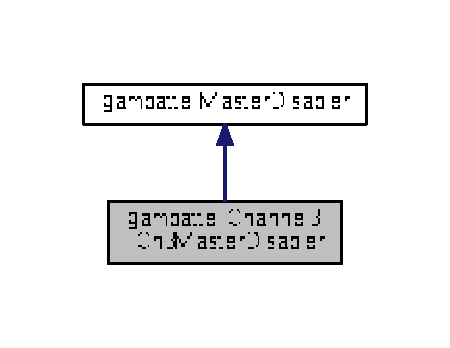
\includegraphics[width=216pt]{classgambatte_1_1Channel3_1_1Ch3MasterDisabler__inherit__graph}
\end{center}
\end{figure}


Collaboration diagram for gambatte\+:\+:Channel3\+:\+:Ch3\+Master\+Disabler\+:
\nopagebreak
\begin{figure}[H]
\begin{center}
\leavevmode
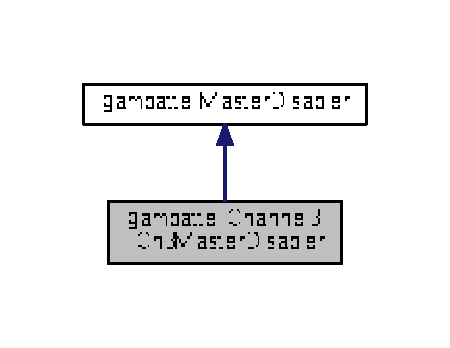
\includegraphics[width=216pt]{classgambatte_1_1Channel3_1_1Ch3MasterDisabler__coll__graph}
\end{center}
\end{figure}
\subsection*{Public Member Functions}
\begin{DoxyCompactItemize}
\item 
\hyperlink{classgambatte_1_1Channel3_1_1Ch3MasterDisabler_a315e8dbc0510e40c248b922c16143196}{Ch3\+Master\+Disabler} (bool \&m, unsigned \&wC)
\item 
virtual void \hyperlink{classgambatte_1_1Channel3_1_1Ch3MasterDisabler_aa8b79b7238fc3249d6a5bb0d64aa43d1}{operator()} ()
\end{DoxyCompactItemize}
\subsection*{Private Attributes}
\begin{DoxyCompactItemize}
\item 
unsigned \& \hyperlink{classgambatte_1_1Channel3_1_1Ch3MasterDisabler_a2b80dcc2777c8a7610b654de40e99440}{wave\+Counter\+\_\+}
\end{DoxyCompactItemize}


\subsection{Constructor \& Destructor Documentation}
\mbox{\Hypertarget{classgambatte_1_1Channel3_1_1Ch3MasterDisabler_a315e8dbc0510e40c248b922c16143196}\label{classgambatte_1_1Channel3_1_1Ch3MasterDisabler_a315e8dbc0510e40c248b922c16143196}} 
\index{gambatte\+::\+Channel3\+::\+Ch3\+Master\+Disabler@{gambatte\+::\+Channel3\+::\+Ch3\+Master\+Disabler}!Ch3\+Master\+Disabler@{Ch3\+Master\+Disabler}}
\index{Ch3\+Master\+Disabler@{Ch3\+Master\+Disabler}!gambatte\+::\+Channel3\+::\+Ch3\+Master\+Disabler@{gambatte\+::\+Channel3\+::\+Ch3\+Master\+Disabler}}
\subsubsection{\texorpdfstring{Ch3\+Master\+Disabler()}{Ch3MasterDisabler()}}
{\footnotesize\ttfamily gambatte\+::\+Channel3\+::\+Ch3\+Master\+Disabler\+::\+Ch3\+Master\+Disabler (\begin{DoxyParamCaption}\item[{bool \&}]{m,  }\item[{unsigned \&}]{wC }\end{DoxyParamCaption})\hspace{0.3cm}{\ttfamily [inline]}}



\subsection{Member Function Documentation}
\mbox{\Hypertarget{classgambatte_1_1Channel3_1_1Ch3MasterDisabler_aa8b79b7238fc3249d6a5bb0d64aa43d1}\label{classgambatte_1_1Channel3_1_1Ch3MasterDisabler_aa8b79b7238fc3249d6a5bb0d64aa43d1}} 
\index{gambatte\+::\+Channel3\+::\+Ch3\+Master\+Disabler@{gambatte\+::\+Channel3\+::\+Ch3\+Master\+Disabler}!operator()@{operator()}}
\index{operator()@{operator()}!gambatte\+::\+Channel3\+::\+Ch3\+Master\+Disabler@{gambatte\+::\+Channel3\+::\+Ch3\+Master\+Disabler}}
\subsubsection{\texorpdfstring{operator()()}{operator()()}}
{\footnotesize\ttfamily virtual void gambatte\+::\+Channel3\+::\+Ch3\+Master\+Disabler\+::operator() (\begin{DoxyParamCaption}{ }\end{DoxyParamCaption})\hspace{0.3cm}{\ttfamily [inline]}, {\ttfamily [virtual]}}



Reimplemented from \hyperlink{classgambatte_1_1MasterDisabler_a6b69f64af3e8112eac3767a74ee0e322}{gambatte\+::\+Master\+Disabler}.



\subsection{Member Data Documentation}
\mbox{\Hypertarget{classgambatte_1_1Channel3_1_1Ch3MasterDisabler_a2b80dcc2777c8a7610b654de40e99440}\label{classgambatte_1_1Channel3_1_1Ch3MasterDisabler_a2b80dcc2777c8a7610b654de40e99440}} 
\index{gambatte\+::\+Channel3\+::\+Ch3\+Master\+Disabler@{gambatte\+::\+Channel3\+::\+Ch3\+Master\+Disabler}!wave\+Counter\+\_\+@{wave\+Counter\+\_\+}}
\index{wave\+Counter\+\_\+@{wave\+Counter\+\_\+}!gambatte\+::\+Channel3\+::\+Ch3\+Master\+Disabler@{gambatte\+::\+Channel3\+::\+Ch3\+Master\+Disabler}}
\subsubsection{\texorpdfstring{wave\+Counter\+\_\+}{waveCounter\_}}
{\footnotesize\ttfamily unsigned\& gambatte\+::\+Channel3\+::\+Ch3\+Master\+Disabler\+::wave\+Counter\+\_\+\hspace{0.3cm}{\ttfamily [private]}}



The documentation for this class was generated from the following file\+:\begin{DoxyCompactItemize}
\item 
src/sound/\hyperlink{channel3_8h}{channel3.\+h}\end{DoxyCompactItemize}

\hypertarget{classgambatte_1_1Channel4_1_1Ch4MasterDisabler}{}\section{gambatte\+:\+:Channel4\+:\+:Ch4\+Master\+Disabler Class Reference}
\label{classgambatte_1_1Channel4_1_1Ch4MasterDisabler}\index{gambatte\+::\+Channel4\+::\+Ch4\+Master\+Disabler@{gambatte\+::\+Channel4\+::\+Ch4\+Master\+Disabler}}


Inheritance diagram for gambatte\+:\+:Channel4\+:\+:Ch4\+Master\+Disabler\+:
\nopagebreak
\begin{figure}[H]
\begin{center}
\leavevmode
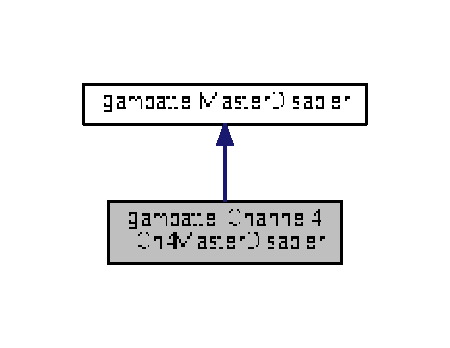
\includegraphics[width=216pt]{classgambatte_1_1Channel4_1_1Ch4MasterDisabler__inherit__graph}
\end{center}
\end{figure}


Collaboration diagram for gambatte\+:\+:Channel4\+:\+:Ch4\+Master\+Disabler\+:
\nopagebreak
\begin{figure}[H]
\begin{center}
\leavevmode
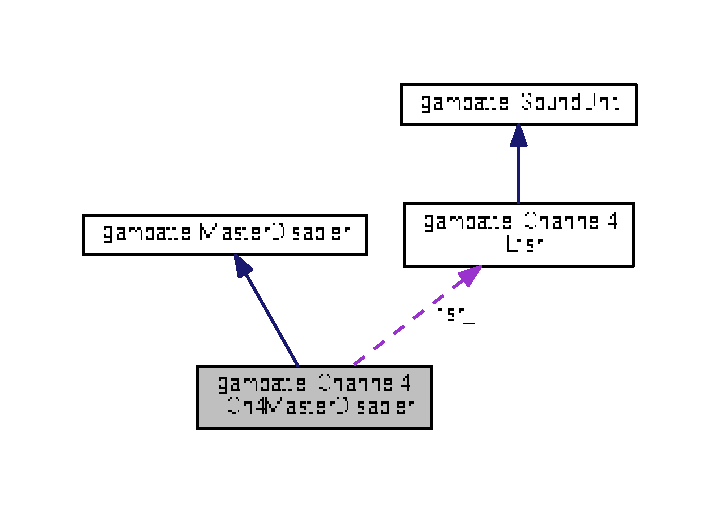
\includegraphics[width=346pt]{classgambatte_1_1Channel4_1_1Ch4MasterDisabler__coll__graph}
\end{center}
\end{figure}
\subsection*{Public Member Functions}
\begin{DoxyCompactItemize}
\item 
\hyperlink{classgambatte_1_1Channel4_1_1Ch4MasterDisabler_a53fe34a1bce0596c36dc917b4e967116}{Ch4\+Master\+Disabler} (bool \&m, \hyperlink{classgambatte_1_1Channel4_1_1Lfsr}{Lfsr} \&lfsr)
\item 
virtual void \hyperlink{classgambatte_1_1Channel4_1_1Ch4MasterDisabler_a7f9ddd23602b991df7ee5bb2a734cc99}{operator()} ()
\end{DoxyCompactItemize}
\subsection*{Private Attributes}
\begin{DoxyCompactItemize}
\item 
\hyperlink{classgambatte_1_1Channel4_1_1Lfsr}{Lfsr} \& \hyperlink{classgambatte_1_1Channel4_1_1Ch4MasterDisabler_a147cca0f452dcbd3df51343e925bac0a}{lfsr\+\_\+}
\end{DoxyCompactItemize}


\subsection{Constructor \& Destructor Documentation}
\mbox{\Hypertarget{classgambatte_1_1Channel4_1_1Ch4MasterDisabler_a53fe34a1bce0596c36dc917b4e967116}\label{classgambatte_1_1Channel4_1_1Ch4MasterDisabler_a53fe34a1bce0596c36dc917b4e967116}} 
\index{gambatte\+::\+Channel4\+::\+Ch4\+Master\+Disabler@{gambatte\+::\+Channel4\+::\+Ch4\+Master\+Disabler}!Ch4\+Master\+Disabler@{Ch4\+Master\+Disabler}}
\index{Ch4\+Master\+Disabler@{Ch4\+Master\+Disabler}!gambatte\+::\+Channel4\+::\+Ch4\+Master\+Disabler@{gambatte\+::\+Channel4\+::\+Ch4\+Master\+Disabler}}
\subsubsection{\texorpdfstring{Ch4\+Master\+Disabler()}{Ch4MasterDisabler()}}
{\footnotesize\ttfamily gambatte\+::\+Channel4\+::\+Ch4\+Master\+Disabler\+::\+Ch4\+Master\+Disabler (\begin{DoxyParamCaption}\item[{bool \&}]{m,  }\item[{\hyperlink{classgambatte_1_1Channel4_1_1Lfsr}{Lfsr} \&}]{lfsr }\end{DoxyParamCaption})\hspace{0.3cm}{\ttfamily [inline]}}



\subsection{Member Function Documentation}
\mbox{\Hypertarget{classgambatte_1_1Channel4_1_1Ch4MasterDisabler_a7f9ddd23602b991df7ee5bb2a734cc99}\label{classgambatte_1_1Channel4_1_1Ch4MasterDisabler_a7f9ddd23602b991df7ee5bb2a734cc99}} 
\index{gambatte\+::\+Channel4\+::\+Ch4\+Master\+Disabler@{gambatte\+::\+Channel4\+::\+Ch4\+Master\+Disabler}!operator()@{operator()}}
\index{operator()@{operator()}!gambatte\+::\+Channel4\+::\+Ch4\+Master\+Disabler@{gambatte\+::\+Channel4\+::\+Ch4\+Master\+Disabler}}
\subsubsection{\texorpdfstring{operator()()}{operator()()}}
{\footnotesize\ttfamily virtual void gambatte\+::\+Channel4\+::\+Ch4\+Master\+Disabler\+::operator() (\begin{DoxyParamCaption}{ }\end{DoxyParamCaption})\hspace{0.3cm}{\ttfamily [inline]}, {\ttfamily [virtual]}}



Reimplemented from \hyperlink{classgambatte_1_1MasterDisabler_a6b69f64af3e8112eac3767a74ee0e322}{gambatte\+::\+Master\+Disabler}.



\subsection{Member Data Documentation}
\mbox{\Hypertarget{classgambatte_1_1Channel4_1_1Ch4MasterDisabler_a147cca0f452dcbd3df51343e925bac0a}\label{classgambatte_1_1Channel4_1_1Ch4MasterDisabler_a147cca0f452dcbd3df51343e925bac0a}} 
\index{gambatte\+::\+Channel4\+::\+Ch4\+Master\+Disabler@{gambatte\+::\+Channel4\+::\+Ch4\+Master\+Disabler}!lfsr\+\_\+@{lfsr\+\_\+}}
\index{lfsr\+\_\+@{lfsr\+\_\+}!gambatte\+::\+Channel4\+::\+Ch4\+Master\+Disabler@{gambatte\+::\+Channel4\+::\+Ch4\+Master\+Disabler}}
\subsubsection{\texorpdfstring{lfsr\+\_\+}{lfsr\_}}
{\footnotesize\ttfamily \hyperlink{classgambatte_1_1Channel4_1_1Lfsr}{Lfsr}\& gambatte\+::\+Channel4\+::\+Ch4\+Master\+Disabler\+::lfsr\+\_\+\hspace{0.3cm}{\ttfamily [private]}}



The documentation for this class was generated from the following file\+:\begin{DoxyCompactItemize}
\item 
src/sound/\hyperlink{channel4_8h}{channel4.\+h}\end{DoxyCompactItemize}

\hypertarget{classgambatte_1_1Channel1}{}\section{gambatte\+:\+:Channel1 Class Reference}
\label{classgambatte_1_1Channel1}\index{gambatte\+::\+Channel1@{gambatte\+::\+Channel1}}


{\ttfamily \#include $<$channel1.\+h$>$}



Collaboration diagram for gambatte\+:\+:Channel1\+:
\nopagebreak
\begin{figure}[H]
\begin{center}
\leavevmode
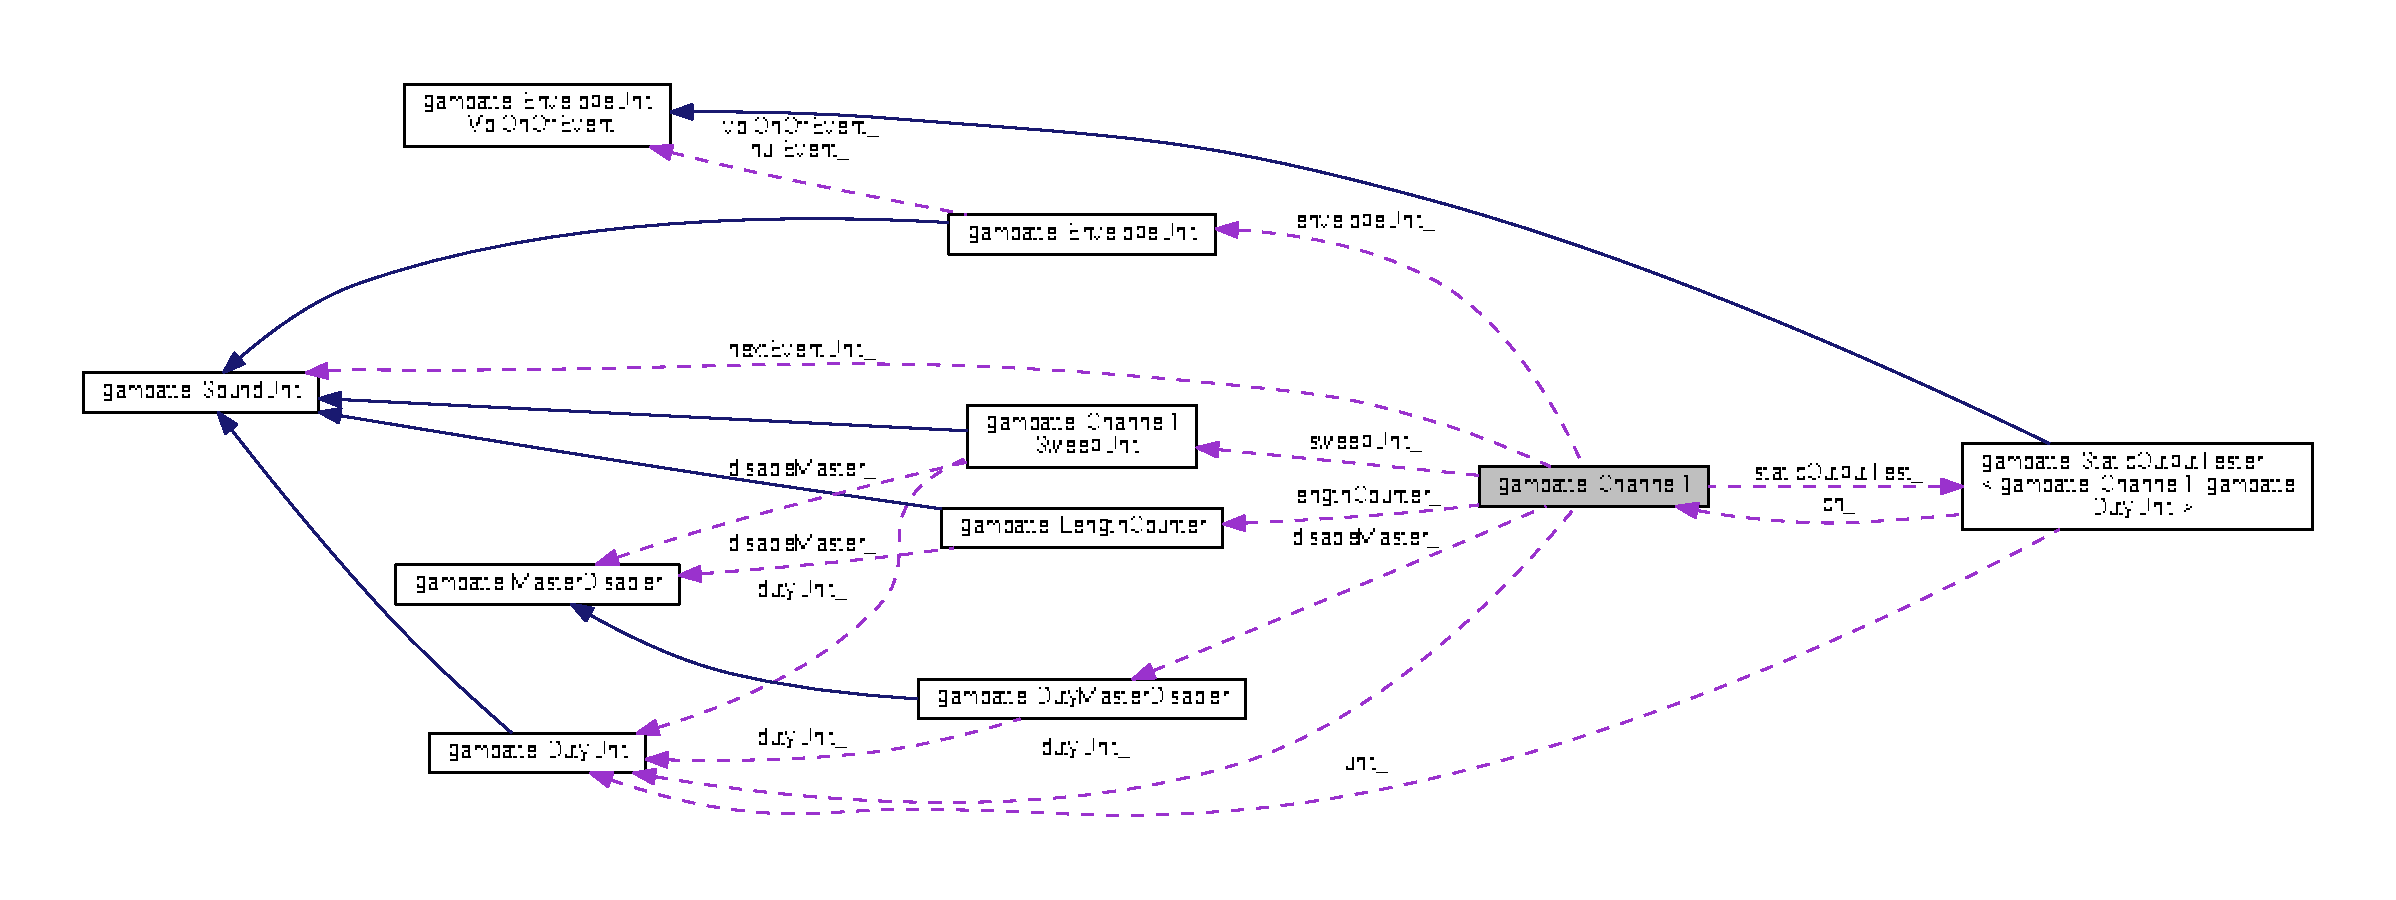
\includegraphics[width=350pt]{classgambatte_1_1Channel1__coll__graph}
\end{center}
\end{figure}
\subsection*{Classes}
\begin{DoxyCompactItemize}
\item 
class \hyperlink{classgambatte_1_1Channel1_1_1SweepUnit}{Sweep\+Unit}
\end{DoxyCompactItemize}
\subsection*{Public Member Functions}
\begin{DoxyCompactItemize}
\item 
\hyperlink{classgambatte_1_1Channel1_af9772f188a3ea499d5ba9d39dbea0545}{Channel1} ()
\item 
void \hyperlink{classgambatte_1_1Channel1_a35804a47c4fdc016ee1b320a504ead57}{set\+Nr0} (unsigned data)
\item 
void \hyperlink{classgambatte_1_1Channel1_ad6f37baaf93cfb198fadec94458ba0eb}{set\+Nr1} (unsigned data)
\item 
void \hyperlink{classgambatte_1_1Channel1_a13d4da832148c21ab5c5089ea89de04f}{set\+Nr2} (unsigned data)
\item 
void \hyperlink{classgambatte_1_1Channel1_aaaef9bf0929047b22e021b100c74667c}{set\+Nr3} (unsigned data)
\item 
void \hyperlink{classgambatte_1_1Channel1_af833ad0df03d687fd907803adeff9280}{set\+Nr4} (unsigned data)
\item 
void \hyperlink{classgambatte_1_1Channel1_ad5868a2f2444ee8275cae4e6f3f9099a}{load\+Or\+Save} (\hyperlink{classgambatte_1_1loadsave}{loadsave} \&\hyperlink{ppu_8cpp_a2f2eca6997ee7baf8901725ae074d45b}{state})
\item 
void \hyperlink{classgambatte_1_1Channel1_a14c458e2f7a0816c658ff9b4453f28a3}{set\+So} (unsigned so\+Mask)
\item 
bool \hyperlink{classgambatte_1_1Channel1_aa40be7480b84da826cc6ec4eec9a4cf8}{is\+Active} () const
\item 
void \hyperlink{classgambatte_1_1Channel1_afaf4543d2bb197c441366e68feac1112}{update} (\hyperlink{namespacegambatte_a0639f09fccfbbd5a8e0796318768e370}{uint\+\_\+least32\+\_\+t} $\ast$\hyperlink{ioapi_8h_a8ad8a13c88886b9f623034ff88570adb}{buf}, unsigned so\+Base\+Vol, unsigned cycles)
\item 
void \hyperlink{classgambatte_1_1Channel1_a734c2e319d5cf2baaee9e23064c55b1b}{reset} ()
\item 
void \hyperlink{classgambatte_1_1Channel1_a91245cfe66613f5243b55cee311564cf}{init} (bool cgb)
\item 
void \hyperlink{classgambatte_1_1Channel1_ac7b4065f024987d29a090fd53771428d}{save\+State} (\hyperlink{structgambatte_1_1SaveState}{Save\+State} \&\hyperlink{ppu_8cpp_a2f2eca6997ee7baf8901725ae074d45b}{state})
\item 
void \hyperlink{classgambatte_1_1Channel1_a156844c5b54cf3cd6ba348064e3b0127}{load\+State} (\hyperlink{structgambatte_1_1SaveState}{Save\+State} const \&\hyperlink{ppu_8cpp_a2f2eca6997ee7baf8901725ae074d45b}{state})
\end{DoxyCompactItemize}
\subsection*{Private Member Functions}
\begin{DoxyCompactItemize}
\item 
void \hyperlink{classgambatte_1_1Channel1_a64fe824b3762fc41959765870518ae00}{set\+Event} ()
\end{DoxyCompactItemize}
\subsection*{Private Attributes}
\begin{DoxyCompactItemize}
\item 
\hyperlink{classgambatte_1_1StaticOutputTester}{Static\+Output\+Tester}$<$ \hyperlink{classgambatte_1_1Channel1}{Channel1}, \hyperlink{classgambatte_1_1DutyUnit}{Duty\+Unit} $>$ \hyperlink{classgambatte_1_1Channel1_ad2a8bb48b34e55b0441785d90ef2de44}{static\+Output\+Test\+\_\+}
\item 
\hyperlink{classgambatte_1_1DutyMasterDisabler}{Duty\+Master\+Disabler} \hyperlink{classgambatte_1_1Channel1_a7a5413ffc80912d4b3919ee9f9558ae9}{disable\+Master\+\_\+}
\item 
\hyperlink{classgambatte_1_1LengthCounter}{Length\+Counter} \hyperlink{classgambatte_1_1Channel1_a778388a95455d724e60d8a967ca6e4d0}{length\+Counter\+\_\+}
\item 
\hyperlink{classgambatte_1_1DutyUnit}{Duty\+Unit} \hyperlink{classgambatte_1_1Channel1_a9a175d5fdcff89f37d8082a37c2a5a75}{duty\+Unit\+\_\+}
\item 
\hyperlink{classgambatte_1_1EnvelopeUnit}{Envelope\+Unit} \hyperlink{classgambatte_1_1Channel1_a3d38d1f11268440dc3af7a048bf5884c}{envelope\+Unit\+\_\+}
\item 
\hyperlink{classgambatte_1_1Channel1_1_1SweepUnit}{Sweep\+Unit} \hyperlink{classgambatte_1_1Channel1_a897acd11661bcfed391947afd5fc3443}{sweep\+Unit\+\_\+}
\item 
\hyperlink{classgambatte_1_1SoundUnit}{Sound\+Unit} $\ast$ \hyperlink{classgambatte_1_1Channel1_aea999f5a312106cc989ee58546675e8b}{next\+Event\+Unit\+\_\+}
\item 
unsigned \hyperlink{classgambatte_1_1Channel1_aab0807b9a067aa4e93a5e103241d60cc}{cycle\+Counter\+\_\+}
\item 
unsigned \hyperlink{classgambatte_1_1Channel1_a7cee0dbdf0287b6a474ad10bf43918a1}{so\+Mask\+\_\+}
\item 
unsigned \hyperlink{classgambatte_1_1Channel1_a337d3fa9640fc3636c958a1deb4a52f8}{prev\+Out\+\_\+}
\item 
unsigned char \hyperlink{classgambatte_1_1Channel1_a1bcfa7f41bfc210dce49fd7bd5493de4}{nr4\+\_\+}
\item 
bool \hyperlink{classgambatte_1_1Channel1_a7a64d3265bbaac73b734104371ec3207}{master\+\_\+}
\end{DoxyCompactItemize}
\subsection*{Friends}
\begin{DoxyCompactItemize}
\item 
class \hyperlink{classgambatte_1_1Channel1_a9aa5c336a7894877fa17f461eb66ddb1}{Static\+Output\+Tester$<$ Channel1, Duty\+Unit $>$}
\end{DoxyCompactItemize}


\subsection{Constructor \& Destructor Documentation}
\mbox{\Hypertarget{classgambatte_1_1Channel1_af9772f188a3ea499d5ba9d39dbea0545}\label{classgambatte_1_1Channel1_af9772f188a3ea499d5ba9d39dbea0545}} 
\index{gambatte\+::\+Channel1@{gambatte\+::\+Channel1}!Channel1@{Channel1}}
\index{Channel1@{Channel1}!gambatte\+::\+Channel1@{gambatte\+::\+Channel1}}
\subsubsection{\texorpdfstring{Channel1()}{Channel1()}}
{\footnotesize\ttfamily gambatte\+::\+Channel1\+::\+Channel1 (\begin{DoxyParamCaption}{ }\end{DoxyParamCaption})}



\subsection{Member Function Documentation}
\mbox{\Hypertarget{classgambatte_1_1Channel1_a91245cfe66613f5243b55cee311564cf}\label{classgambatte_1_1Channel1_a91245cfe66613f5243b55cee311564cf}} 
\index{gambatte\+::\+Channel1@{gambatte\+::\+Channel1}!init@{init}}
\index{init@{init}!gambatte\+::\+Channel1@{gambatte\+::\+Channel1}}
\subsubsection{\texorpdfstring{init()}{init()}}
{\footnotesize\ttfamily void gambatte\+::\+Channel1\+::init (\begin{DoxyParamCaption}\item[{bool}]{cgb }\end{DoxyParamCaption})}

\mbox{\Hypertarget{classgambatte_1_1Channel1_aa40be7480b84da826cc6ec4eec9a4cf8}\label{classgambatte_1_1Channel1_aa40be7480b84da826cc6ec4eec9a4cf8}} 
\index{gambatte\+::\+Channel1@{gambatte\+::\+Channel1}!is\+Active@{is\+Active}}
\index{is\+Active@{is\+Active}!gambatte\+::\+Channel1@{gambatte\+::\+Channel1}}
\subsubsection{\texorpdfstring{is\+Active()}{isActive()}}
{\footnotesize\ttfamily bool gambatte\+::\+Channel1\+::is\+Active (\begin{DoxyParamCaption}{ }\end{DoxyParamCaption}) const\hspace{0.3cm}{\ttfamily [inline]}}

\mbox{\Hypertarget{classgambatte_1_1Channel1_ad5868a2f2444ee8275cae4e6f3f9099a}\label{classgambatte_1_1Channel1_ad5868a2f2444ee8275cae4e6f3f9099a}} 
\index{gambatte\+::\+Channel1@{gambatte\+::\+Channel1}!load\+Or\+Save@{load\+Or\+Save}}
\index{load\+Or\+Save@{load\+Or\+Save}!gambatte\+::\+Channel1@{gambatte\+::\+Channel1}}
\subsubsection{\texorpdfstring{load\+Or\+Save()}{loadOrSave()}}
{\footnotesize\ttfamily void gambatte\+::\+Channel1\+::load\+Or\+Save (\begin{DoxyParamCaption}\item[{\hyperlink{classgambatte_1_1loadsave}{loadsave} \&}]{state }\end{DoxyParamCaption})}

\mbox{\Hypertarget{classgambatte_1_1Channel1_a156844c5b54cf3cd6ba348064e3b0127}\label{classgambatte_1_1Channel1_a156844c5b54cf3cd6ba348064e3b0127}} 
\index{gambatte\+::\+Channel1@{gambatte\+::\+Channel1}!load\+State@{load\+State}}
\index{load\+State@{load\+State}!gambatte\+::\+Channel1@{gambatte\+::\+Channel1}}
\subsubsection{\texorpdfstring{load\+State()}{loadState()}}
{\footnotesize\ttfamily void gambatte\+::\+Channel1\+::load\+State (\begin{DoxyParamCaption}\item[{\hyperlink{structgambatte_1_1SaveState}{Save\+State} const \&}]{state }\end{DoxyParamCaption})}

\mbox{\Hypertarget{classgambatte_1_1Channel1_a734c2e319d5cf2baaee9e23064c55b1b}\label{classgambatte_1_1Channel1_a734c2e319d5cf2baaee9e23064c55b1b}} 
\index{gambatte\+::\+Channel1@{gambatte\+::\+Channel1}!reset@{reset}}
\index{reset@{reset}!gambatte\+::\+Channel1@{gambatte\+::\+Channel1}}
\subsubsection{\texorpdfstring{reset()}{reset()}}
{\footnotesize\ttfamily void gambatte\+::\+Channel1\+::reset (\begin{DoxyParamCaption}{ }\end{DoxyParamCaption})}

\mbox{\Hypertarget{classgambatte_1_1Channel1_ac7b4065f024987d29a090fd53771428d}\label{classgambatte_1_1Channel1_ac7b4065f024987d29a090fd53771428d}} 
\index{gambatte\+::\+Channel1@{gambatte\+::\+Channel1}!save\+State@{save\+State}}
\index{save\+State@{save\+State}!gambatte\+::\+Channel1@{gambatte\+::\+Channel1}}
\subsubsection{\texorpdfstring{save\+State()}{saveState()}}
{\footnotesize\ttfamily void gambatte\+::\+Channel1\+::save\+State (\begin{DoxyParamCaption}\item[{\hyperlink{structgambatte_1_1SaveState}{Save\+State} \&}]{state }\end{DoxyParamCaption})}

\mbox{\Hypertarget{classgambatte_1_1Channel1_a64fe824b3762fc41959765870518ae00}\label{classgambatte_1_1Channel1_a64fe824b3762fc41959765870518ae00}} 
\index{gambatte\+::\+Channel1@{gambatte\+::\+Channel1}!set\+Event@{set\+Event}}
\index{set\+Event@{set\+Event}!gambatte\+::\+Channel1@{gambatte\+::\+Channel1}}
\subsubsection{\texorpdfstring{set\+Event()}{setEvent()}}
{\footnotesize\ttfamily void gambatte\+::\+Channel1\+::set\+Event (\begin{DoxyParamCaption}{ }\end{DoxyParamCaption})\hspace{0.3cm}{\ttfamily [private]}}

\mbox{\Hypertarget{classgambatte_1_1Channel1_a35804a47c4fdc016ee1b320a504ead57}\label{classgambatte_1_1Channel1_a35804a47c4fdc016ee1b320a504ead57}} 
\index{gambatte\+::\+Channel1@{gambatte\+::\+Channel1}!set\+Nr0@{set\+Nr0}}
\index{set\+Nr0@{set\+Nr0}!gambatte\+::\+Channel1@{gambatte\+::\+Channel1}}
\subsubsection{\texorpdfstring{set\+Nr0()}{setNr0()}}
{\footnotesize\ttfamily void gambatte\+::\+Channel1\+::set\+Nr0 (\begin{DoxyParamCaption}\item[{unsigned}]{data }\end{DoxyParamCaption})}

\mbox{\Hypertarget{classgambatte_1_1Channel1_ad6f37baaf93cfb198fadec94458ba0eb}\label{classgambatte_1_1Channel1_ad6f37baaf93cfb198fadec94458ba0eb}} 
\index{gambatte\+::\+Channel1@{gambatte\+::\+Channel1}!set\+Nr1@{set\+Nr1}}
\index{set\+Nr1@{set\+Nr1}!gambatte\+::\+Channel1@{gambatte\+::\+Channel1}}
\subsubsection{\texorpdfstring{set\+Nr1()}{setNr1()}}
{\footnotesize\ttfamily void gambatte\+::\+Channel1\+::set\+Nr1 (\begin{DoxyParamCaption}\item[{unsigned}]{data }\end{DoxyParamCaption})}

\mbox{\Hypertarget{classgambatte_1_1Channel1_a13d4da832148c21ab5c5089ea89de04f}\label{classgambatte_1_1Channel1_a13d4da832148c21ab5c5089ea89de04f}} 
\index{gambatte\+::\+Channel1@{gambatte\+::\+Channel1}!set\+Nr2@{set\+Nr2}}
\index{set\+Nr2@{set\+Nr2}!gambatte\+::\+Channel1@{gambatte\+::\+Channel1}}
\subsubsection{\texorpdfstring{set\+Nr2()}{setNr2()}}
{\footnotesize\ttfamily void gambatte\+::\+Channel1\+::set\+Nr2 (\begin{DoxyParamCaption}\item[{unsigned}]{data }\end{DoxyParamCaption})}

\mbox{\Hypertarget{classgambatte_1_1Channel1_aaaef9bf0929047b22e021b100c74667c}\label{classgambatte_1_1Channel1_aaaef9bf0929047b22e021b100c74667c}} 
\index{gambatte\+::\+Channel1@{gambatte\+::\+Channel1}!set\+Nr3@{set\+Nr3}}
\index{set\+Nr3@{set\+Nr3}!gambatte\+::\+Channel1@{gambatte\+::\+Channel1}}
\subsubsection{\texorpdfstring{set\+Nr3()}{setNr3()}}
{\footnotesize\ttfamily void gambatte\+::\+Channel1\+::set\+Nr3 (\begin{DoxyParamCaption}\item[{unsigned}]{data }\end{DoxyParamCaption})}

\mbox{\Hypertarget{classgambatte_1_1Channel1_af833ad0df03d687fd907803adeff9280}\label{classgambatte_1_1Channel1_af833ad0df03d687fd907803adeff9280}} 
\index{gambatte\+::\+Channel1@{gambatte\+::\+Channel1}!set\+Nr4@{set\+Nr4}}
\index{set\+Nr4@{set\+Nr4}!gambatte\+::\+Channel1@{gambatte\+::\+Channel1}}
\subsubsection{\texorpdfstring{set\+Nr4()}{setNr4()}}
{\footnotesize\ttfamily void gambatte\+::\+Channel1\+::set\+Nr4 (\begin{DoxyParamCaption}\item[{unsigned}]{data }\end{DoxyParamCaption})}

\mbox{\Hypertarget{classgambatte_1_1Channel1_a14c458e2f7a0816c658ff9b4453f28a3}\label{classgambatte_1_1Channel1_a14c458e2f7a0816c658ff9b4453f28a3}} 
\index{gambatte\+::\+Channel1@{gambatte\+::\+Channel1}!set\+So@{set\+So}}
\index{set\+So@{set\+So}!gambatte\+::\+Channel1@{gambatte\+::\+Channel1}}
\subsubsection{\texorpdfstring{set\+So()}{setSo()}}
{\footnotesize\ttfamily void gambatte\+::\+Channel1\+::set\+So (\begin{DoxyParamCaption}\item[{unsigned}]{so\+Mask }\end{DoxyParamCaption})}

\mbox{\Hypertarget{classgambatte_1_1Channel1_afaf4543d2bb197c441366e68feac1112}\label{classgambatte_1_1Channel1_afaf4543d2bb197c441366e68feac1112}} 
\index{gambatte\+::\+Channel1@{gambatte\+::\+Channel1}!update@{update}}
\index{update@{update}!gambatte\+::\+Channel1@{gambatte\+::\+Channel1}}
\subsubsection{\texorpdfstring{update()}{update()}}
{\footnotesize\ttfamily void gambatte\+::\+Channel1\+::update (\begin{DoxyParamCaption}\item[{\hyperlink{namespacegambatte_a0639f09fccfbbd5a8e0796318768e370}{uint\+\_\+least32\+\_\+t} $\ast$}]{buf,  }\item[{unsigned}]{so\+Base\+Vol,  }\item[{unsigned}]{cycles }\end{DoxyParamCaption})}



\subsection{Friends And Related Function Documentation}
\mbox{\Hypertarget{classgambatte_1_1Channel1_a9aa5c336a7894877fa17f461eb66ddb1}\label{classgambatte_1_1Channel1_a9aa5c336a7894877fa17f461eb66ddb1}} 
\index{gambatte\+::\+Channel1@{gambatte\+::\+Channel1}!Static\+Output\+Tester$<$ Channel1, Duty\+Unit $>$@{Static\+Output\+Tester$<$ Channel1, Duty\+Unit $>$}}
\index{Static\+Output\+Tester$<$ Channel1, Duty\+Unit $>$@{Static\+Output\+Tester$<$ Channel1, Duty\+Unit $>$}!gambatte\+::\+Channel1@{gambatte\+::\+Channel1}}
\subsubsection{\texorpdfstring{Static\+Output\+Tester$<$ Channel1, Duty\+Unit $>$}{StaticOutputTester< Channel1, DutyUnit >}}
{\footnotesize\ttfamily friend class \hyperlink{classgambatte_1_1StaticOutputTester}{Static\+Output\+Tester}$<$ \hyperlink{classgambatte_1_1Channel1}{Channel1}, \hyperlink{classgambatte_1_1DutyUnit}{Duty\+Unit} $>$\hspace{0.3cm}{\ttfamily [friend]}}



\subsection{Member Data Documentation}
\mbox{\Hypertarget{classgambatte_1_1Channel1_aab0807b9a067aa4e93a5e103241d60cc}\label{classgambatte_1_1Channel1_aab0807b9a067aa4e93a5e103241d60cc}} 
\index{gambatte\+::\+Channel1@{gambatte\+::\+Channel1}!cycle\+Counter\+\_\+@{cycle\+Counter\+\_\+}}
\index{cycle\+Counter\+\_\+@{cycle\+Counter\+\_\+}!gambatte\+::\+Channel1@{gambatte\+::\+Channel1}}
\subsubsection{\texorpdfstring{cycle\+Counter\+\_\+}{cycleCounter\_}}
{\footnotesize\ttfamily unsigned gambatte\+::\+Channel1\+::cycle\+Counter\+\_\+\hspace{0.3cm}{\ttfamily [private]}}

\mbox{\Hypertarget{classgambatte_1_1Channel1_a7a5413ffc80912d4b3919ee9f9558ae9}\label{classgambatte_1_1Channel1_a7a5413ffc80912d4b3919ee9f9558ae9}} 
\index{gambatte\+::\+Channel1@{gambatte\+::\+Channel1}!disable\+Master\+\_\+@{disable\+Master\+\_\+}}
\index{disable\+Master\+\_\+@{disable\+Master\+\_\+}!gambatte\+::\+Channel1@{gambatte\+::\+Channel1}}
\subsubsection{\texorpdfstring{disable\+Master\+\_\+}{disableMaster\_}}
{\footnotesize\ttfamily \hyperlink{classgambatte_1_1DutyMasterDisabler}{Duty\+Master\+Disabler} gambatte\+::\+Channel1\+::disable\+Master\+\_\+\hspace{0.3cm}{\ttfamily [private]}}

\mbox{\Hypertarget{classgambatte_1_1Channel1_a9a175d5fdcff89f37d8082a37c2a5a75}\label{classgambatte_1_1Channel1_a9a175d5fdcff89f37d8082a37c2a5a75}} 
\index{gambatte\+::\+Channel1@{gambatte\+::\+Channel1}!duty\+Unit\+\_\+@{duty\+Unit\+\_\+}}
\index{duty\+Unit\+\_\+@{duty\+Unit\+\_\+}!gambatte\+::\+Channel1@{gambatte\+::\+Channel1}}
\subsubsection{\texorpdfstring{duty\+Unit\+\_\+}{dutyUnit\_}}
{\footnotesize\ttfamily \hyperlink{classgambatte_1_1DutyUnit}{Duty\+Unit} gambatte\+::\+Channel1\+::duty\+Unit\+\_\+\hspace{0.3cm}{\ttfamily [private]}}

\mbox{\Hypertarget{classgambatte_1_1Channel1_a3d38d1f11268440dc3af7a048bf5884c}\label{classgambatte_1_1Channel1_a3d38d1f11268440dc3af7a048bf5884c}} 
\index{gambatte\+::\+Channel1@{gambatte\+::\+Channel1}!envelope\+Unit\+\_\+@{envelope\+Unit\+\_\+}}
\index{envelope\+Unit\+\_\+@{envelope\+Unit\+\_\+}!gambatte\+::\+Channel1@{gambatte\+::\+Channel1}}
\subsubsection{\texorpdfstring{envelope\+Unit\+\_\+}{envelopeUnit\_}}
{\footnotesize\ttfamily \hyperlink{classgambatte_1_1EnvelopeUnit}{Envelope\+Unit} gambatte\+::\+Channel1\+::envelope\+Unit\+\_\+\hspace{0.3cm}{\ttfamily [private]}}

\mbox{\Hypertarget{classgambatte_1_1Channel1_a778388a95455d724e60d8a967ca6e4d0}\label{classgambatte_1_1Channel1_a778388a95455d724e60d8a967ca6e4d0}} 
\index{gambatte\+::\+Channel1@{gambatte\+::\+Channel1}!length\+Counter\+\_\+@{length\+Counter\+\_\+}}
\index{length\+Counter\+\_\+@{length\+Counter\+\_\+}!gambatte\+::\+Channel1@{gambatte\+::\+Channel1}}
\subsubsection{\texorpdfstring{length\+Counter\+\_\+}{lengthCounter\_}}
{\footnotesize\ttfamily \hyperlink{classgambatte_1_1LengthCounter}{Length\+Counter} gambatte\+::\+Channel1\+::length\+Counter\+\_\+\hspace{0.3cm}{\ttfamily [private]}}

\mbox{\Hypertarget{classgambatte_1_1Channel1_a7a64d3265bbaac73b734104371ec3207}\label{classgambatte_1_1Channel1_a7a64d3265bbaac73b734104371ec3207}} 
\index{gambatte\+::\+Channel1@{gambatte\+::\+Channel1}!master\+\_\+@{master\+\_\+}}
\index{master\+\_\+@{master\+\_\+}!gambatte\+::\+Channel1@{gambatte\+::\+Channel1}}
\subsubsection{\texorpdfstring{master\+\_\+}{master\_}}
{\footnotesize\ttfamily bool gambatte\+::\+Channel1\+::master\+\_\+\hspace{0.3cm}{\ttfamily [private]}}

\mbox{\Hypertarget{classgambatte_1_1Channel1_aea999f5a312106cc989ee58546675e8b}\label{classgambatte_1_1Channel1_aea999f5a312106cc989ee58546675e8b}} 
\index{gambatte\+::\+Channel1@{gambatte\+::\+Channel1}!next\+Event\+Unit\+\_\+@{next\+Event\+Unit\+\_\+}}
\index{next\+Event\+Unit\+\_\+@{next\+Event\+Unit\+\_\+}!gambatte\+::\+Channel1@{gambatte\+::\+Channel1}}
\subsubsection{\texorpdfstring{next\+Event\+Unit\+\_\+}{nextEventUnit\_}}
{\footnotesize\ttfamily \hyperlink{classgambatte_1_1SoundUnit}{Sound\+Unit}$\ast$ gambatte\+::\+Channel1\+::next\+Event\+Unit\+\_\+\hspace{0.3cm}{\ttfamily [private]}}

\mbox{\Hypertarget{classgambatte_1_1Channel1_a1bcfa7f41bfc210dce49fd7bd5493de4}\label{classgambatte_1_1Channel1_a1bcfa7f41bfc210dce49fd7bd5493de4}} 
\index{gambatte\+::\+Channel1@{gambatte\+::\+Channel1}!nr4\+\_\+@{nr4\+\_\+}}
\index{nr4\+\_\+@{nr4\+\_\+}!gambatte\+::\+Channel1@{gambatte\+::\+Channel1}}
\subsubsection{\texorpdfstring{nr4\+\_\+}{nr4\_}}
{\footnotesize\ttfamily unsigned char gambatte\+::\+Channel1\+::nr4\+\_\+\hspace{0.3cm}{\ttfamily [private]}}

\mbox{\Hypertarget{classgambatte_1_1Channel1_a337d3fa9640fc3636c958a1deb4a52f8}\label{classgambatte_1_1Channel1_a337d3fa9640fc3636c958a1deb4a52f8}} 
\index{gambatte\+::\+Channel1@{gambatte\+::\+Channel1}!prev\+Out\+\_\+@{prev\+Out\+\_\+}}
\index{prev\+Out\+\_\+@{prev\+Out\+\_\+}!gambatte\+::\+Channel1@{gambatte\+::\+Channel1}}
\subsubsection{\texorpdfstring{prev\+Out\+\_\+}{prevOut\_}}
{\footnotesize\ttfamily unsigned gambatte\+::\+Channel1\+::prev\+Out\+\_\+\hspace{0.3cm}{\ttfamily [private]}}

\mbox{\Hypertarget{classgambatte_1_1Channel1_a7cee0dbdf0287b6a474ad10bf43918a1}\label{classgambatte_1_1Channel1_a7cee0dbdf0287b6a474ad10bf43918a1}} 
\index{gambatte\+::\+Channel1@{gambatte\+::\+Channel1}!so\+Mask\+\_\+@{so\+Mask\+\_\+}}
\index{so\+Mask\+\_\+@{so\+Mask\+\_\+}!gambatte\+::\+Channel1@{gambatte\+::\+Channel1}}
\subsubsection{\texorpdfstring{so\+Mask\+\_\+}{soMask\_}}
{\footnotesize\ttfamily unsigned gambatte\+::\+Channel1\+::so\+Mask\+\_\+\hspace{0.3cm}{\ttfamily [private]}}

\mbox{\Hypertarget{classgambatte_1_1Channel1_ad2a8bb48b34e55b0441785d90ef2de44}\label{classgambatte_1_1Channel1_ad2a8bb48b34e55b0441785d90ef2de44}} 
\index{gambatte\+::\+Channel1@{gambatte\+::\+Channel1}!static\+Output\+Test\+\_\+@{static\+Output\+Test\+\_\+}}
\index{static\+Output\+Test\+\_\+@{static\+Output\+Test\+\_\+}!gambatte\+::\+Channel1@{gambatte\+::\+Channel1}}
\subsubsection{\texorpdfstring{static\+Output\+Test\+\_\+}{staticOutputTest\_}}
{\footnotesize\ttfamily \hyperlink{classgambatte_1_1StaticOutputTester}{Static\+Output\+Tester}$<$\hyperlink{classgambatte_1_1Channel1}{Channel1}, \hyperlink{classgambatte_1_1DutyUnit}{Duty\+Unit}$>$ gambatte\+::\+Channel1\+::static\+Output\+Test\+\_\+\hspace{0.3cm}{\ttfamily [private]}}

\mbox{\Hypertarget{classgambatte_1_1Channel1_a897acd11661bcfed391947afd5fc3443}\label{classgambatte_1_1Channel1_a897acd11661bcfed391947afd5fc3443}} 
\index{gambatte\+::\+Channel1@{gambatte\+::\+Channel1}!sweep\+Unit\+\_\+@{sweep\+Unit\+\_\+}}
\index{sweep\+Unit\+\_\+@{sweep\+Unit\+\_\+}!gambatte\+::\+Channel1@{gambatte\+::\+Channel1}}
\subsubsection{\texorpdfstring{sweep\+Unit\+\_\+}{sweepUnit\_}}
{\footnotesize\ttfamily \hyperlink{classgambatte_1_1Channel1_1_1SweepUnit}{Sweep\+Unit} gambatte\+::\+Channel1\+::sweep\+Unit\+\_\+\hspace{0.3cm}{\ttfamily [private]}}



The documentation for this class was generated from the following files\+:\begin{DoxyCompactItemize}
\item 
src/sound/\hyperlink{channel1_8h}{channel1.\+h}\item 
src/sound/\hyperlink{channel1_8cpp}{channel1.\+cpp}\end{DoxyCompactItemize}

\hypertarget{classgambatte_1_1Channel2}{}\section{gambatte\+:\+:Channel2 Class Reference}
\label{classgambatte_1_1Channel2}\index{gambatte\+::\+Channel2@{gambatte\+::\+Channel2}}


{\ttfamily \#include $<$channel2.\+h$>$}



Collaboration diagram for gambatte\+:\+:Channel2\+:
\nopagebreak
\begin{figure}[H]
\begin{center}
\leavevmode
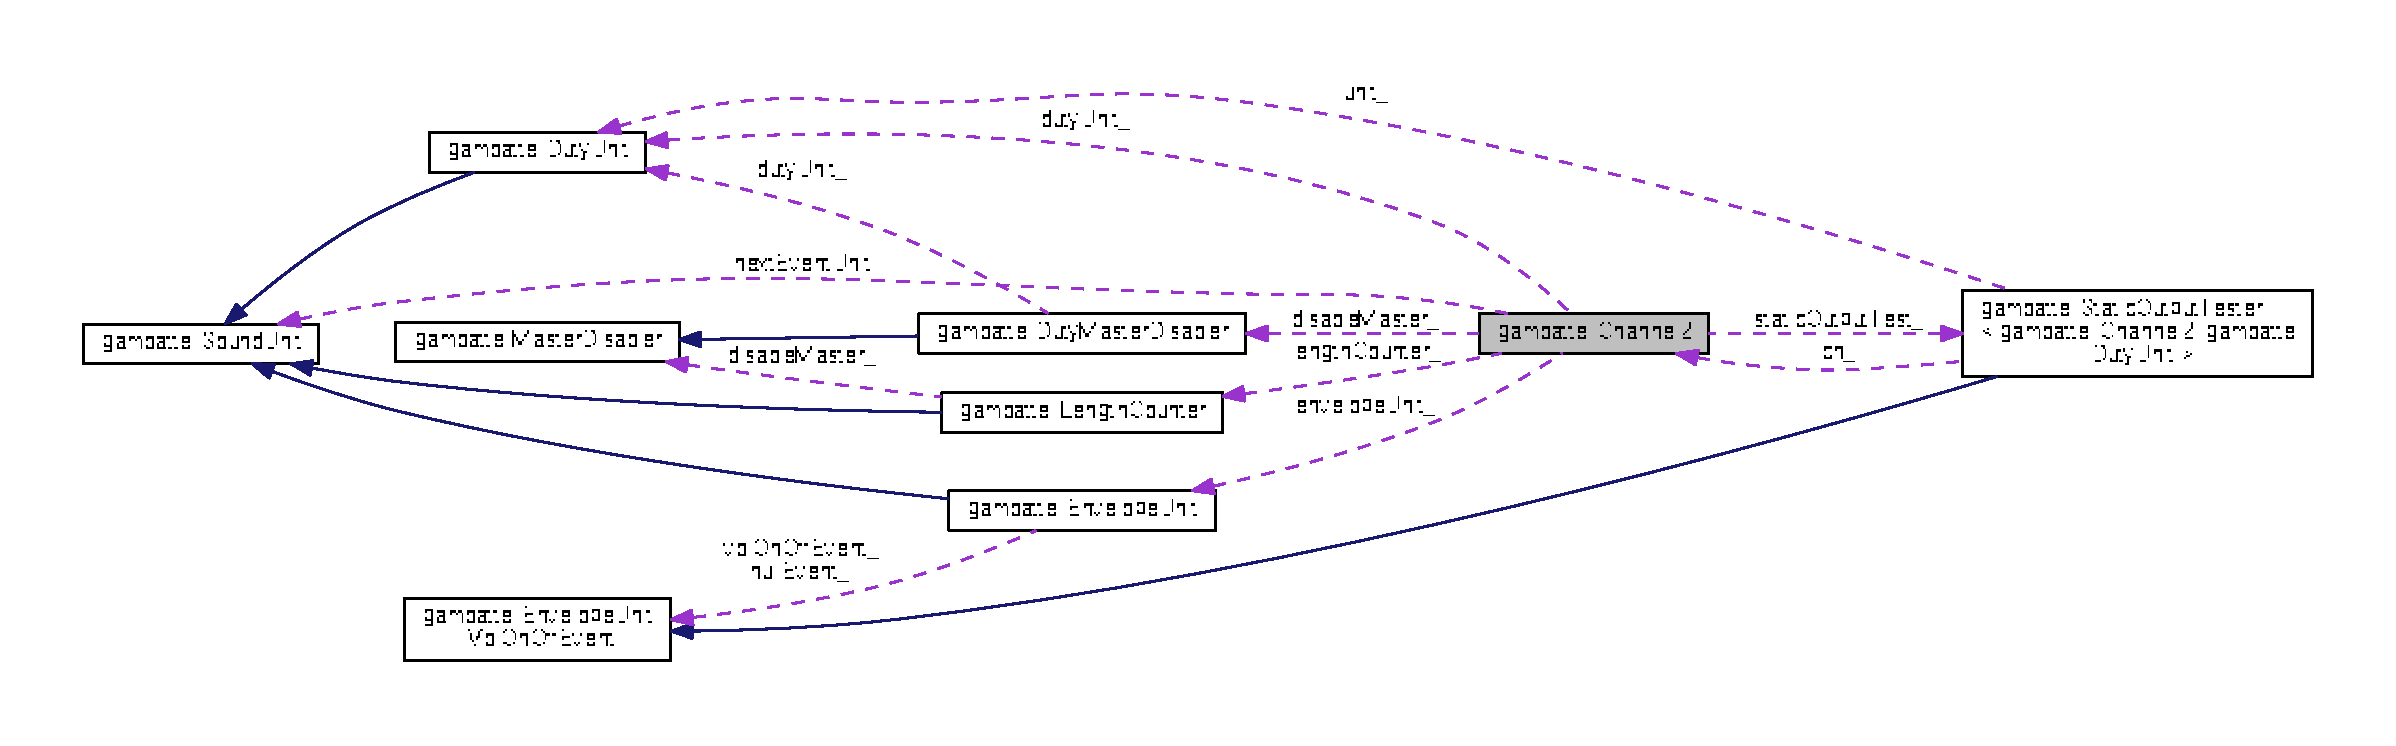
\includegraphics[width=350pt]{classgambatte_1_1Channel2__coll__graph}
\end{center}
\end{figure}
\subsection*{Public Member Functions}
\begin{DoxyCompactItemize}
\item 
\hyperlink{classgambatte_1_1Channel2_a9439edf10073a5eac15556cd503d0182}{Channel2} ()
\item 
void \hyperlink{classgambatte_1_1Channel2_a77f0fdaa9b46038ece53181518bdb2cf}{set\+Nr1} (unsigned data)
\item 
void \hyperlink{classgambatte_1_1Channel2_a510e5b62ec5f2b64396aacb554bcfe99}{set\+Nr2} (unsigned data)
\item 
void \hyperlink{classgambatte_1_1Channel2_a1ef8b568dcd73da7dfbfe141098827fe}{set\+Nr3} (unsigned data)
\item 
void \hyperlink{classgambatte_1_1Channel2_a56454c49f4fed868967b30f6779e78da}{set\+Nr4} (unsigned data)
\item 
void \hyperlink{classgambatte_1_1Channel2_a49323ba3b0f4c200538c785fdce2d371}{load\+Or\+Save} (\hyperlink{classgambatte_1_1loadsave}{loadsave} \&\hyperlink{ppu_8cpp_a2f2eca6997ee7baf8901725ae074d45b}{state})
\item 
void \hyperlink{classgambatte_1_1Channel2_a63d7445c20fc635f6bbc28b51c17c690}{set\+So} (unsigned so\+Mask)
\item 
bool \hyperlink{classgambatte_1_1Channel2_a866214a53810c25c810ca09855aa4e7c}{is\+Active} () const
\item 
void \hyperlink{classgambatte_1_1Channel2_a017f34d58c36f89f8b3f64a552e3b31e}{update} (\hyperlink{namespacegambatte_a0639f09fccfbbd5a8e0796318768e370}{uint\+\_\+least32\+\_\+t} $\ast$\hyperlink{ioapi_8h_a8ad8a13c88886b9f623034ff88570adb}{buf}, unsigned so\+Base\+Vol, unsigned cycles)
\item 
void \hyperlink{classgambatte_1_1Channel2_a41bfbf50f1d123c43d5b5317ec73387a}{reset} ()
\item 
void \hyperlink{classgambatte_1_1Channel2_a10af65cdd99207c851a00ce7b15245ab}{init} (bool cgb)
\item 
void \hyperlink{classgambatte_1_1Channel2_a65e1566e37749fa686bf5f607fc10161}{save\+State} (\hyperlink{structgambatte_1_1SaveState}{Save\+State} \&\hyperlink{ppu_8cpp_a2f2eca6997ee7baf8901725ae074d45b}{state})
\item 
void \hyperlink{classgambatte_1_1Channel2_a22a07432a95ad31fdec2f9e7b1ef6f97}{load\+State} (\hyperlink{structgambatte_1_1SaveState}{Save\+State} const \&\hyperlink{ppu_8cpp_a2f2eca6997ee7baf8901725ae074d45b}{state})
\end{DoxyCompactItemize}
\subsection*{Private Member Functions}
\begin{DoxyCompactItemize}
\item 
void \hyperlink{classgambatte_1_1Channel2_aef1eba3499906c82587cbd0eb5121e5f}{set\+Event} ()
\end{DoxyCompactItemize}
\subsection*{Private Attributes}
\begin{DoxyCompactItemize}
\item 
\hyperlink{classgambatte_1_1StaticOutputTester}{Static\+Output\+Tester}$<$ \hyperlink{classgambatte_1_1Channel2}{Channel2}, \hyperlink{classgambatte_1_1DutyUnit}{Duty\+Unit} $>$ \hyperlink{classgambatte_1_1Channel2_ade1b5b7d5517320d0a92a5ae0b1af918}{static\+Output\+Test\+\_\+}
\item 
\hyperlink{classgambatte_1_1DutyMasterDisabler}{Duty\+Master\+Disabler} \hyperlink{classgambatte_1_1Channel2_a456784be1b1e094c67e0fa70eecadcd4}{disable\+Master\+\_\+}
\item 
\hyperlink{classgambatte_1_1LengthCounter}{Length\+Counter} \hyperlink{classgambatte_1_1Channel2_aefd094a39e4c8b1a2da1472b85d07861}{length\+Counter\+\_\+}
\item 
\hyperlink{classgambatte_1_1DutyUnit}{Duty\+Unit} \hyperlink{classgambatte_1_1Channel2_a611db79f91b08849e774831891f813d2}{duty\+Unit\+\_\+}
\item 
\hyperlink{classgambatte_1_1EnvelopeUnit}{Envelope\+Unit} \hyperlink{classgambatte_1_1Channel2_a66c56b6990b18999d03129b296165ffc}{envelope\+Unit\+\_\+}
\item 
\hyperlink{classgambatte_1_1SoundUnit}{Sound\+Unit} $\ast$ \hyperlink{classgambatte_1_1Channel2_a575a4077c57d48dbe7f5a6a433c65a78}{next\+Event\+Unit}
\item 
unsigned \hyperlink{classgambatte_1_1Channel2_aecc04331c16f6c32b35ac1094adc7c6c}{cycle\+Counter\+\_\+}
\item 
unsigned \hyperlink{classgambatte_1_1Channel2_ad25cd68978e87a67fb8a68403a7ec921}{so\+Mask\+\_\+}
\item 
unsigned \hyperlink{classgambatte_1_1Channel2_ad897ba192b5c1cd32970e87016c75a29}{prev\+Out\+\_\+}
\item 
unsigned char \hyperlink{classgambatte_1_1Channel2_a4e215e5ebf51ebd69f67847aedba4409}{nr4\+\_\+}
\item 
bool \hyperlink{classgambatte_1_1Channel2_a90a3ad5dba4a1c3630aa702dc90b3428}{master\+\_\+}
\end{DoxyCompactItemize}
\subsection*{Friends}
\begin{DoxyCompactItemize}
\item 
class \hyperlink{classgambatte_1_1Channel2_a0e4bb4e43d3269e56a11539381699ad0}{Static\+Output\+Tester$<$ Channel2, Duty\+Unit $>$}
\end{DoxyCompactItemize}


\subsection{Constructor \& Destructor Documentation}
\mbox{\Hypertarget{classgambatte_1_1Channel2_a9439edf10073a5eac15556cd503d0182}\label{classgambatte_1_1Channel2_a9439edf10073a5eac15556cd503d0182}} 
\index{gambatte\+::\+Channel2@{gambatte\+::\+Channel2}!Channel2@{Channel2}}
\index{Channel2@{Channel2}!gambatte\+::\+Channel2@{gambatte\+::\+Channel2}}
\subsubsection{\texorpdfstring{Channel2()}{Channel2()}}
{\footnotesize\ttfamily gambatte\+::\+Channel2\+::\+Channel2 (\begin{DoxyParamCaption}{ }\end{DoxyParamCaption})}



\subsection{Member Function Documentation}
\mbox{\Hypertarget{classgambatte_1_1Channel2_a10af65cdd99207c851a00ce7b15245ab}\label{classgambatte_1_1Channel2_a10af65cdd99207c851a00ce7b15245ab}} 
\index{gambatte\+::\+Channel2@{gambatte\+::\+Channel2}!init@{init}}
\index{init@{init}!gambatte\+::\+Channel2@{gambatte\+::\+Channel2}}
\subsubsection{\texorpdfstring{init()}{init()}}
{\footnotesize\ttfamily void gambatte\+::\+Channel2\+::init (\begin{DoxyParamCaption}\item[{bool}]{cgb }\end{DoxyParamCaption})}

\mbox{\Hypertarget{classgambatte_1_1Channel2_a866214a53810c25c810ca09855aa4e7c}\label{classgambatte_1_1Channel2_a866214a53810c25c810ca09855aa4e7c}} 
\index{gambatte\+::\+Channel2@{gambatte\+::\+Channel2}!is\+Active@{is\+Active}}
\index{is\+Active@{is\+Active}!gambatte\+::\+Channel2@{gambatte\+::\+Channel2}}
\subsubsection{\texorpdfstring{is\+Active()}{isActive()}}
{\footnotesize\ttfamily bool gambatte\+::\+Channel2\+::is\+Active (\begin{DoxyParamCaption}{ }\end{DoxyParamCaption}) const\hspace{0.3cm}{\ttfamily [inline]}}

\mbox{\Hypertarget{classgambatte_1_1Channel2_a49323ba3b0f4c200538c785fdce2d371}\label{classgambatte_1_1Channel2_a49323ba3b0f4c200538c785fdce2d371}} 
\index{gambatte\+::\+Channel2@{gambatte\+::\+Channel2}!load\+Or\+Save@{load\+Or\+Save}}
\index{load\+Or\+Save@{load\+Or\+Save}!gambatte\+::\+Channel2@{gambatte\+::\+Channel2}}
\subsubsection{\texorpdfstring{load\+Or\+Save()}{loadOrSave()}}
{\footnotesize\ttfamily void gambatte\+::\+Channel2\+::load\+Or\+Save (\begin{DoxyParamCaption}\item[{\hyperlink{classgambatte_1_1loadsave}{loadsave} \&}]{state }\end{DoxyParamCaption})}

\mbox{\Hypertarget{classgambatte_1_1Channel2_a22a07432a95ad31fdec2f9e7b1ef6f97}\label{classgambatte_1_1Channel2_a22a07432a95ad31fdec2f9e7b1ef6f97}} 
\index{gambatte\+::\+Channel2@{gambatte\+::\+Channel2}!load\+State@{load\+State}}
\index{load\+State@{load\+State}!gambatte\+::\+Channel2@{gambatte\+::\+Channel2}}
\subsubsection{\texorpdfstring{load\+State()}{loadState()}}
{\footnotesize\ttfamily void gambatte\+::\+Channel2\+::load\+State (\begin{DoxyParamCaption}\item[{\hyperlink{structgambatte_1_1SaveState}{Save\+State} const \&}]{state }\end{DoxyParamCaption})}

\mbox{\Hypertarget{classgambatte_1_1Channel2_a41bfbf50f1d123c43d5b5317ec73387a}\label{classgambatte_1_1Channel2_a41bfbf50f1d123c43d5b5317ec73387a}} 
\index{gambatte\+::\+Channel2@{gambatte\+::\+Channel2}!reset@{reset}}
\index{reset@{reset}!gambatte\+::\+Channel2@{gambatte\+::\+Channel2}}
\subsubsection{\texorpdfstring{reset()}{reset()}}
{\footnotesize\ttfamily void gambatte\+::\+Channel2\+::reset (\begin{DoxyParamCaption}{ }\end{DoxyParamCaption})}

\mbox{\Hypertarget{classgambatte_1_1Channel2_a65e1566e37749fa686bf5f607fc10161}\label{classgambatte_1_1Channel2_a65e1566e37749fa686bf5f607fc10161}} 
\index{gambatte\+::\+Channel2@{gambatte\+::\+Channel2}!save\+State@{save\+State}}
\index{save\+State@{save\+State}!gambatte\+::\+Channel2@{gambatte\+::\+Channel2}}
\subsubsection{\texorpdfstring{save\+State()}{saveState()}}
{\footnotesize\ttfamily void gambatte\+::\+Channel2\+::save\+State (\begin{DoxyParamCaption}\item[{\hyperlink{structgambatte_1_1SaveState}{Save\+State} \&}]{state }\end{DoxyParamCaption})}

\mbox{\Hypertarget{classgambatte_1_1Channel2_aef1eba3499906c82587cbd0eb5121e5f}\label{classgambatte_1_1Channel2_aef1eba3499906c82587cbd0eb5121e5f}} 
\index{gambatte\+::\+Channel2@{gambatte\+::\+Channel2}!set\+Event@{set\+Event}}
\index{set\+Event@{set\+Event}!gambatte\+::\+Channel2@{gambatte\+::\+Channel2}}
\subsubsection{\texorpdfstring{set\+Event()}{setEvent()}}
{\footnotesize\ttfamily void gambatte\+::\+Channel2\+::set\+Event (\begin{DoxyParamCaption}{ }\end{DoxyParamCaption})\hspace{0.3cm}{\ttfamily [private]}}

\mbox{\Hypertarget{classgambatte_1_1Channel2_a77f0fdaa9b46038ece53181518bdb2cf}\label{classgambatte_1_1Channel2_a77f0fdaa9b46038ece53181518bdb2cf}} 
\index{gambatte\+::\+Channel2@{gambatte\+::\+Channel2}!set\+Nr1@{set\+Nr1}}
\index{set\+Nr1@{set\+Nr1}!gambatte\+::\+Channel2@{gambatte\+::\+Channel2}}
\subsubsection{\texorpdfstring{set\+Nr1()}{setNr1()}}
{\footnotesize\ttfamily void gambatte\+::\+Channel2\+::set\+Nr1 (\begin{DoxyParamCaption}\item[{unsigned}]{data }\end{DoxyParamCaption})}

\mbox{\Hypertarget{classgambatte_1_1Channel2_a510e5b62ec5f2b64396aacb554bcfe99}\label{classgambatte_1_1Channel2_a510e5b62ec5f2b64396aacb554bcfe99}} 
\index{gambatte\+::\+Channel2@{gambatte\+::\+Channel2}!set\+Nr2@{set\+Nr2}}
\index{set\+Nr2@{set\+Nr2}!gambatte\+::\+Channel2@{gambatte\+::\+Channel2}}
\subsubsection{\texorpdfstring{set\+Nr2()}{setNr2()}}
{\footnotesize\ttfamily void gambatte\+::\+Channel2\+::set\+Nr2 (\begin{DoxyParamCaption}\item[{unsigned}]{data }\end{DoxyParamCaption})}

\mbox{\Hypertarget{classgambatte_1_1Channel2_a1ef8b568dcd73da7dfbfe141098827fe}\label{classgambatte_1_1Channel2_a1ef8b568dcd73da7dfbfe141098827fe}} 
\index{gambatte\+::\+Channel2@{gambatte\+::\+Channel2}!set\+Nr3@{set\+Nr3}}
\index{set\+Nr3@{set\+Nr3}!gambatte\+::\+Channel2@{gambatte\+::\+Channel2}}
\subsubsection{\texorpdfstring{set\+Nr3()}{setNr3()}}
{\footnotesize\ttfamily void gambatte\+::\+Channel2\+::set\+Nr3 (\begin{DoxyParamCaption}\item[{unsigned}]{data }\end{DoxyParamCaption})}

\mbox{\Hypertarget{classgambatte_1_1Channel2_a56454c49f4fed868967b30f6779e78da}\label{classgambatte_1_1Channel2_a56454c49f4fed868967b30f6779e78da}} 
\index{gambatte\+::\+Channel2@{gambatte\+::\+Channel2}!set\+Nr4@{set\+Nr4}}
\index{set\+Nr4@{set\+Nr4}!gambatte\+::\+Channel2@{gambatte\+::\+Channel2}}
\subsubsection{\texorpdfstring{set\+Nr4()}{setNr4()}}
{\footnotesize\ttfamily void gambatte\+::\+Channel2\+::set\+Nr4 (\begin{DoxyParamCaption}\item[{unsigned}]{data }\end{DoxyParamCaption})}

\mbox{\Hypertarget{classgambatte_1_1Channel2_a63d7445c20fc635f6bbc28b51c17c690}\label{classgambatte_1_1Channel2_a63d7445c20fc635f6bbc28b51c17c690}} 
\index{gambatte\+::\+Channel2@{gambatte\+::\+Channel2}!set\+So@{set\+So}}
\index{set\+So@{set\+So}!gambatte\+::\+Channel2@{gambatte\+::\+Channel2}}
\subsubsection{\texorpdfstring{set\+So()}{setSo()}}
{\footnotesize\ttfamily void gambatte\+::\+Channel2\+::set\+So (\begin{DoxyParamCaption}\item[{unsigned}]{so\+Mask }\end{DoxyParamCaption})}

\mbox{\Hypertarget{classgambatte_1_1Channel2_a017f34d58c36f89f8b3f64a552e3b31e}\label{classgambatte_1_1Channel2_a017f34d58c36f89f8b3f64a552e3b31e}} 
\index{gambatte\+::\+Channel2@{gambatte\+::\+Channel2}!update@{update}}
\index{update@{update}!gambatte\+::\+Channel2@{gambatte\+::\+Channel2}}
\subsubsection{\texorpdfstring{update()}{update()}}
{\footnotesize\ttfamily void gambatte\+::\+Channel2\+::update (\begin{DoxyParamCaption}\item[{\hyperlink{namespacegambatte_a0639f09fccfbbd5a8e0796318768e370}{uint\+\_\+least32\+\_\+t} $\ast$}]{buf,  }\item[{unsigned}]{so\+Base\+Vol,  }\item[{unsigned}]{cycles }\end{DoxyParamCaption})}



\subsection{Friends And Related Function Documentation}
\mbox{\Hypertarget{classgambatte_1_1Channel2_a0e4bb4e43d3269e56a11539381699ad0}\label{classgambatte_1_1Channel2_a0e4bb4e43d3269e56a11539381699ad0}} 
\index{gambatte\+::\+Channel2@{gambatte\+::\+Channel2}!Static\+Output\+Tester$<$ Channel2, Duty\+Unit $>$@{Static\+Output\+Tester$<$ Channel2, Duty\+Unit $>$}}
\index{Static\+Output\+Tester$<$ Channel2, Duty\+Unit $>$@{Static\+Output\+Tester$<$ Channel2, Duty\+Unit $>$}!gambatte\+::\+Channel2@{gambatte\+::\+Channel2}}
\subsubsection{\texorpdfstring{Static\+Output\+Tester$<$ Channel2, Duty\+Unit $>$}{StaticOutputTester< Channel2, DutyUnit >}}
{\footnotesize\ttfamily friend class \hyperlink{classgambatte_1_1StaticOutputTester}{Static\+Output\+Tester}$<$ \hyperlink{classgambatte_1_1Channel2}{Channel2}, \hyperlink{classgambatte_1_1DutyUnit}{Duty\+Unit} $>$\hspace{0.3cm}{\ttfamily [friend]}}



\subsection{Member Data Documentation}
\mbox{\Hypertarget{classgambatte_1_1Channel2_aecc04331c16f6c32b35ac1094adc7c6c}\label{classgambatte_1_1Channel2_aecc04331c16f6c32b35ac1094adc7c6c}} 
\index{gambatte\+::\+Channel2@{gambatte\+::\+Channel2}!cycle\+Counter\+\_\+@{cycle\+Counter\+\_\+}}
\index{cycle\+Counter\+\_\+@{cycle\+Counter\+\_\+}!gambatte\+::\+Channel2@{gambatte\+::\+Channel2}}
\subsubsection{\texorpdfstring{cycle\+Counter\+\_\+}{cycleCounter\_}}
{\footnotesize\ttfamily unsigned gambatte\+::\+Channel2\+::cycle\+Counter\+\_\+\hspace{0.3cm}{\ttfamily [private]}}

\mbox{\Hypertarget{classgambatte_1_1Channel2_a456784be1b1e094c67e0fa70eecadcd4}\label{classgambatte_1_1Channel2_a456784be1b1e094c67e0fa70eecadcd4}} 
\index{gambatte\+::\+Channel2@{gambatte\+::\+Channel2}!disable\+Master\+\_\+@{disable\+Master\+\_\+}}
\index{disable\+Master\+\_\+@{disable\+Master\+\_\+}!gambatte\+::\+Channel2@{gambatte\+::\+Channel2}}
\subsubsection{\texorpdfstring{disable\+Master\+\_\+}{disableMaster\_}}
{\footnotesize\ttfamily \hyperlink{classgambatte_1_1DutyMasterDisabler}{Duty\+Master\+Disabler} gambatte\+::\+Channel2\+::disable\+Master\+\_\+\hspace{0.3cm}{\ttfamily [private]}}

\mbox{\Hypertarget{classgambatte_1_1Channel2_a611db79f91b08849e774831891f813d2}\label{classgambatte_1_1Channel2_a611db79f91b08849e774831891f813d2}} 
\index{gambatte\+::\+Channel2@{gambatte\+::\+Channel2}!duty\+Unit\+\_\+@{duty\+Unit\+\_\+}}
\index{duty\+Unit\+\_\+@{duty\+Unit\+\_\+}!gambatte\+::\+Channel2@{gambatte\+::\+Channel2}}
\subsubsection{\texorpdfstring{duty\+Unit\+\_\+}{dutyUnit\_}}
{\footnotesize\ttfamily \hyperlink{classgambatte_1_1DutyUnit}{Duty\+Unit} gambatte\+::\+Channel2\+::duty\+Unit\+\_\+\hspace{0.3cm}{\ttfamily [private]}}

\mbox{\Hypertarget{classgambatte_1_1Channel2_a66c56b6990b18999d03129b296165ffc}\label{classgambatte_1_1Channel2_a66c56b6990b18999d03129b296165ffc}} 
\index{gambatte\+::\+Channel2@{gambatte\+::\+Channel2}!envelope\+Unit\+\_\+@{envelope\+Unit\+\_\+}}
\index{envelope\+Unit\+\_\+@{envelope\+Unit\+\_\+}!gambatte\+::\+Channel2@{gambatte\+::\+Channel2}}
\subsubsection{\texorpdfstring{envelope\+Unit\+\_\+}{envelopeUnit\_}}
{\footnotesize\ttfamily \hyperlink{classgambatte_1_1EnvelopeUnit}{Envelope\+Unit} gambatte\+::\+Channel2\+::envelope\+Unit\+\_\+\hspace{0.3cm}{\ttfamily [private]}}

\mbox{\Hypertarget{classgambatte_1_1Channel2_aefd094a39e4c8b1a2da1472b85d07861}\label{classgambatte_1_1Channel2_aefd094a39e4c8b1a2da1472b85d07861}} 
\index{gambatte\+::\+Channel2@{gambatte\+::\+Channel2}!length\+Counter\+\_\+@{length\+Counter\+\_\+}}
\index{length\+Counter\+\_\+@{length\+Counter\+\_\+}!gambatte\+::\+Channel2@{gambatte\+::\+Channel2}}
\subsubsection{\texorpdfstring{length\+Counter\+\_\+}{lengthCounter\_}}
{\footnotesize\ttfamily \hyperlink{classgambatte_1_1LengthCounter}{Length\+Counter} gambatte\+::\+Channel2\+::length\+Counter\+\_\+\hspace{0.3cm}{\ttfamily [private]}}

\mbox{\Hypertarget{classgambatte_1_1Channel2_a90a3ad5dba4a1c3630aa702dc90b3428}\label{classgambatte_1_1Channel2_a90a3ad5dba4a1c3630aa702dc90b3428}} 
\index{gambatte\+::\+Channel2@{gambatte\+::\+Channel2}!master\+\_\+@{master\+\_\+}}
\index{master\+\_\+@{master\+\_\+}!gambatte\+::\+Channel2@{gambatte\+::\+Channel2}}
\subsubsection{\texorpdfstring{master\+\_\+}{master\_}}
{\footnotesize\ttfamily bool gambatte\+::\+Channel2\+::master\+\_\+\hspace{0.3cm}{\ttfamily [private]}}

\mbox{\Hypertarget{classgambatte_1_1Channel2_a575a4077c57d48dbe7f5a6a433c65a78}\label{classgambatte_1_1Channel2_a575a4077c57d48dbe7f5a6a433c65a78}} 
\index{gambatte\+::\+Channel2@{gambatte\+::\+Channel2}!next\+Event\+Unit@{next\+Event\+Unit}}
\index{next\+Event\+Unit@{next\+Event\+Unit}!gambatte\+::\+Channel2@{gambatte\+::\+Channel2}}
\subsubsection{\texorpdfstring{next\+Event\+Unit}{nextEventUnit}}
{\footnotesize\ttfamily \hyperlink{classgambatte_1_1SoundUnit}{Sound\+Unit}$\ast$ gambatte\+::\+Channel2\+::next\+Event\+Unit\hspace{0.3cm}{\ttfamily [private]}}

\mbox{\Hypertarget{classgambatte_1_1Channel2_a4e215e5ebf51ebd69f67847aedba4409}\label{classgambatte_1_1Channel2_a4e215e5ebf51ebd69f67847aedba4409}} 
\index{gambatte\+::\+Channel2@{gambatte\+::\+Channel2}!nr4\+\_\+@{nr4\+\_\+}}
\index{nr4\+\_\+@{nr4\+\_\+}!gambatte\+::\+Channel2@{gambatte\+::\+Channel2}}
\subsubsection{\texorpdfstring{nr4\+\_\+}{nr4\_}}
{\footnotesize\ttfamily unsigned char gambatte\+::\+Channel2\+::nr4\+\_\+\hspace{0.3cm}{\ttfamily [private]}}

\mbox{\Hypertarget{classgambatte_1_1Channel2_ad897ba192b5c1cd32970e87016c75a29}\label{classgambatte_1_1Channel2_ad897ba192b5c1cd32970e87016c75a29}} 
\index{gambatte\+::\+Channel2@{gambatte\+::\+Channel2}!prev\+Out\+\_\+@{prev\+Out\+\_\+}}
\index{prev\+Out\+\_\+@{prev\+Out\+\_\+}!gambatte\+::\+Channel2@{gambatte\+::\+Channel2}}
\subsubsection{\texorpdfstring{prev\+Out\+\_\+}{prevOut\_}}
{\footnotesize\ttfamily unsigned gambatte\+::\+Channel2\+::prev\+Out\+\_\+\hspace{0.3cm}{\ttfamily [private]}}

\mbox{\Hypertarget{classgambatte_1_1Channel2_ad25cd68978e87a67fb8a68403a7ec921}\label{classgambatte_1_1Channel2_ad25cd68978e87a67fb8a68403a7ec921}} 
\index{gambatte\+::\+Channel2@{gambatte\+::\+Channel2}!so\+Mask\+\_\+@{so\+Mask\+\_\+}}
\index{so\+Mask\+\_\+@{so\+Mask\+\_\+}!gambatte\+::\+Channel2@{gambatte\+::\+Channel2}}
\subsubsection{\texorpdfstring{so\+Mask\+\_\+}{soMask\_}}
{\footnotesize\ttfamily unsigned gambatte\+::\+Channel2\+::so\+Mask\+\_\+\hspace{0.3cm}{\ttfamily [private]}}

\mbox{\Hypertarget{classgambatte_1_1Channel2_ade1b5b7d5517320d0a92a5ae0b1af918}\label{classgambatte_1_1Channel2_ade1b5b7d5517320d0a92a5ae0b1af918}} 
\index{gambatte\+::\+Channel2@{gambatte\+::\+Channel2}!static\+Output\+Test\+\_\+@{static\+Output\+Test\+\_\+}}
\index{static\+Output\+Test\+\_\+@{static\+Output\+Test\+\_\+}!gambatte\+::\+Channel2@{gambatte\+::\+Channel2}}
\subsubsection{\texorpdfstring{static\+Output\+Test\+\_\+}{staticOutputTest\_}}
{\footnotesize\ttfamily \hyperlink{classgambatte_1_1StaticOutputTester}{Static\+Output\+Tester}$<$\hyperlink{classgambatte_1_1Channel2}{Channel2}, \hyperlink{classgambatte_1_1DutyUnit}{Duty\+Unit}$>$ gambatte\+::\+Channel2\+::static\+Output\+Test\+\_\+\hspace{0.3cm}{\ttfamily [private]}}



The documentation for this class was generated from the following files\+:\begin{DoxyCompactItemize}
\item 
src/sound/\hyperlink{channel2_8h}{channel2.\+h}\item 
src/sound/\hyperlink{channel2_8cpp}{channel2.\+cpp}\end{DoxyCompactItemize}

\hypertarget{classgambatte_1_1Channel3}{}\section{gambatte\+:\+:Channel3 Class Reference}
\label{classgambatte_1_1Channel3}\index{gambatte\+::\+Channel3@{gambatte\+::\+Channel3}}


{\ttfamily \#include $<$channel3.\+h$>$}



Collaboration diagram for gambatte\+:\+:Channel3\+:
\nopagebreak
\begin{figure}[H]
\begin{center}
\leavevmode
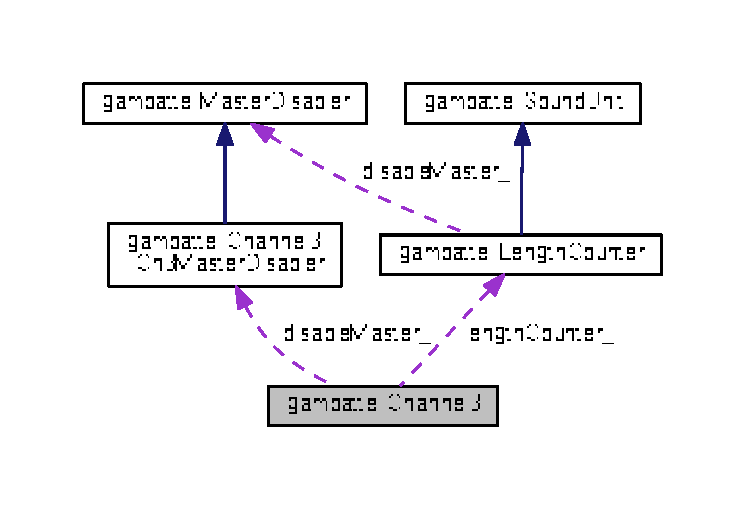
\includegraphics[width=350pt]{classgambatte_1_1Channel3__coll__graph}
\end{center}
\end{figure}
\subsection*{Classes}
\begin{DoxyCompactItemize}
\item 
class \hyperlink{classgambatte_1_1Channel3_1_1Ch3MasterDisabler}{Ch3\+Master\+Disabler}
\end{DoxyCompactItemize}
\subsection*{Public Member Functions}
\begin{DoxyCompactItemize}
\item 
\hyperlink{classgambatte_1_1Channel3_a9c7d0995ebc9f8d6ff78e97136723588}{Channel3} ()
\item 
bool \hyperlink{classgambatte_1_1Channel3_a8c90742b546acc34949544dfdc5e3a06}{is\+Active} () const
\item 
void \hyperlink{classgambatte_1_1Channel3_a2b249e82410f1a623835328e27b52c0f}{reset} ()
\item 
void \hyperlink{classgambatte_1_1Channel3_a960fd026f9cc424f495f4c3557b17c38}{init} (bool cgb)
\item 
void \hyperlink{classgambatte_1_1Channel3_a4e5c1b827c38e28362cd736a12cd1324}{set\+State\+Ptrs} (\hyperlink{structgambatte_1_1SaveState}{Save\+State} \&\hyperlink{ppu_8cpp_a2f2eca6997ee7baf8901725ae074d45b}{state})
\item 
void \hyperlink{classgambatte_1_1Channel3_a3a1442523f6196ad8e031445e5b46256}{save\+State} (\hyperlink{structgambatte_1_1SaveState}{Save\+State} \&\hyperlink{ppu_8cpp_a2f2eca6997ee7baf8901725ae074d45b}{state}) const
\item 
void \hyperlink{classgambatte_1_1Channel3_aaa317622a29cb8e71cdce44178961839}{load\+State} (const \hyperlink{structgambatte_1_1SaveState}{Save\+State} \&\hyperlink{ppu_8cpp_a2f2eca6997ee7baf8901725ae074d45b}{state})
\item 
void \hyperlink{classgambatte_1_1Channel3_ac54d37c29e7a35ab2394fe185f796758}{set\+Nr0} (unsigned data)
\item 
void \hyperlink{classgambatte_1_1Channel3_a4530b1049b8ba6e64c761a286b605f6f}{set\+Nr1} (unsigned data)
\item 
void \hyperlink{classgambatte_1_1Channel3_abf6fece5005b23c8accc5a6f9af62a39}{set\+Nr2} (unsigned data)
\item 
void \hyperlink{classgambatte_1_1Channel3_a7e992093a461b59d1ca4922788f94823}{set\+Nr3} (unsigned data)
\item 
void \hyperlink{classgambatte_1_1Channel3_aab1312c2b2883934096d1a274bf118c4}{set\+Nr4} (unsigned data)
\item 
void \hyperlink{classgambatte_1_1Channel3_a8d95b16d980a90f284ea05c650a53212}{set\+So} (unsigned so\+Mask)
\item 
void \hyperlink{classgambatte_1_1Channel3_a2d3d845741694ae103cb7d60d87dbeb5}{update} (\hyperlink{namespacegambatte_a0639f09fccfbbd5a8e0796318768e370}{uint\+\_\+least32\+\_\+t} $\ast$\hyperlink{ioapi_8h_a8ad8a13c88886b9f623034ff88570adb}{buf}, unsigned so\+Base\+Vol, unsigned cycles)
\item 
unsigned \hyperlink{classgambatte_1_1Channel3_aaab70bedfa5561f68bf8b562b9bbec07}{wave\+Ram\+Read} (unsigned index) const
\item 
void \hyperlink{classgambatte_1_1Channel3_ae4dfc2534984a5255816a9383c2c0307}{wave\+Ram\+Write} (unsigned index, unsigned data)
\item 
void \hyperlink{classgambatte_1_1Channel3_affe1d4cd442fb9cbdfef697ad6dbcd2b}{load\+Or\+Save} (\hyperlink{classgambatte_1_1loadsave}{loadsave} \&\hyperlink{ppu_8cpp_a2f2eca6997ee7baf8901725ae074d45b}{state})
\end{DoxyCompactItemize}
\subsection*{Private Member Functions}
\begin{DoxyCompactItemize}
\item 
void \hyperlink{classgambatte_1_1Channel3_a3ac9a519fecd48cd847de615afabbf3d}{update\+Wave\+Counter} (unsigned cc)
\end{DoxyCompactItemize}
\subsection*{Private Attributes}
\begin{DoxyCompactItemize}
\item 
unsigned char \hyperlink{classgambatte_1_1Channel3_adb49da0eed0e8e9fc7e7d67d88bf71f8}{wave\+Ram\+\_\+} \mbox{[}0x10\mbox{]}
\item 
\hyperlink{classgambatte_1_1Channel3_1_1Ch3MasterDisabler}{Ch3\+Master\+Disabler} \hyperlink{classgambatte_1_1Channel3_a449cc9afb7108dbecadfe2aee64eca7e}{disable\+Master\+\_\+}
\item 
\hyperlink{classgambatte_1_1LengthCounter}{Length\+Counter} \hyperlink{classgambatte_1_1Channel3_a2ea56b70d73fa7004bf5a4eb9b39538d}{length\+Counter\+\_\+}
\item 
unsigned \hyperlink{classgambatte_1_1Channel3_af06cab780d1d050d555889e0d3a44420}{cycle\+Counter\+\_\+}
\item 
unsigned \hyperlink{classgambatte_1_1Channel3_a4c5d31731f34309766d7b0e1267b45a0}{so\+Mask\+\_\+}
\item 
unsigned \hyperlink{classgambatte_1_1Channel3_a9cf0ee95ea065667f05600b1f5e49220}{prev\+Out\+\_\+}
\item 
unsigned \hyperlink{classgambatte_1_1Channel3_aeac32dfe75b7162668161acf3b50af34}{wave\+Counter\+\_\+}
\item 
unsigned \hyperlink{classgambatte_1_1Channel3_af4d0a88ee0abb8add35441c75963e29c}{last\+Read\+Time\+\_\+}
\item 
unsigned char \hyperlink{classgambatte_1_1Channel3_a7dc08776d608a4eeb23d0d121a3ea820}{nr0\+\_\+}
\item 
unsigned char \hyperlink{classgambatte_1_1Channel3_a253cc1dae94d72525c73015a5ca44f40}{nr3\+\_\+}
\item 
unsigned char \hyperlink{classgambatte_1_1Channel3_a7f60fafcf33ac8cc5bfe343f83695f07}{nr4\+\_\+}
\item 
unsigned char \hyperlink{classgambatte_1_1Channel3_a92f41b6ef5d3d3578e59597392db0eca}{wave\+Pos\+\_\+}
\item 
unsigned char \hyperlink{classgambatte_1_1Channel3_a043ba215cf9dfb925b26e231df26a77c}{rshift\+\_\+}
\item 
unsigned char \hyperlink{classgambatte_1_1Channel3_a958b59a4d8db55242588f76e0a7c7137}{sample\+Buf\+\_\+}
\item 
bool \hyperlink{classgambatte_1_1Channel3_aa4267f127e7aaa01a8cb8fcbd25d4f21}{master\+\_\+}
\item 
bool \hyperlink{classgambatte_1_1Channel3_a44558d0f698be5e911181a36b35d4e66}{cgb\+\_\+}
\end{DoxyCompactItemize}


\subsection{Constructor \& Destructor Documentation}
\mbox{\Hypertarget{classgambatte_1_1Channel3_a9c7d0995ebc9f8d6ff78e97136723588}\label{classgambatte_1_1Channel3_a9c7d0995ebc9f8d6ff78e97136723588}} 
\index{gambatte\+::\+Channel3@{gambatte\+::\+Channel3}!Channel3@{Channel3}}
\index{Channel3@{Channel3}!gambatte\+::\+Channel3@{gambatte\+::\+Channel3}}
\subsubsection{\texorpdfstring{Channel3()}{Channel3()}}
{\footnotesize\ttfamily gambatte\+::\+Channel3\+::\+Channel3 (\begin{DoxyParamCaption}{ }\end{DoxyParamCaption})}



\subsection{Member Function Documentation}
\mbox{\Hypertarget{classgambatte_1_1Channel3_a960fd026f9cc424f495f4c3557b17c38}\label{classgambatte_1_1Channel3_a960fd026f9cc424f495f4c3557b17c38}} 
\index{gambatte\+::\+Channel3@{gambatte\+::\+Channel3}!init@{init}}
\index{init@{init}!gambatte\+::\+Channel3@{gambatte\+::\+Channel3}}
\subsubsection{\texorpdfstring{init()}{init()}}
{\footnotesize\ttfamily void gambatte\+::\+Channel3\+::init (\begin{DoxyParamCaption}\item[{bool}]{cgb }\end{DoxyParamCaption})}

\mbox{\Hypertarget{classgambatte_1_1Channel3_a8c90742b546acc34949544dfdc5e3a06}\label{classgambatte_1_1Channel3_a8c90742b546acc34949544dfdc5e3a06}} 
\index{gambatte\+::\+Channel3@{gambatte\+::\+Channel3}!is\+Active@{is\+Active}}
\index{is\+Active@{is\+Active}!gambatte\+::\+Channel3@{gambatte\+::\+Channel3}}
\subsubsection{\texorpdfstring{is\+Active()}{isActive()}}
{\footnotesize\ttfamily bool gambatte\+::\+Channel3\+::is\+Active (\begin{DoxyParamCaption}{ }\end{DoxyParamCaption}) const\hspace{0.3cm}{\ttfamily [inline]}}

\mbox{\Hypertarget{classgambatte_1_1Channel3_affe1d4cd442fb9cbdfef697ad6dbcd2b}\label{classgambatte_1_1Channel3_affe1d4cd442fb9cbdfef697ad6dbcd2b}} 
\index{gambatte\+::\+Channel3@{gambatte\+::\+Channel3}!load\+Or\+Save@{load\+Or\+Save}}
\index{load\+Or\+Save@{load\+Or\+Save}!gambatte\+::\+Channel3@{gambatte\+::\+Channel3}}
\subsubsection{\texorpdfstring{load\+Or\+Save()}{loadOrSave()}}
{\footnotesize\ttfamily void gambatte\+::\+Channel3\+::load\+Or\+Save (\begin{DoxyParamCaption}\item[{\hyperlink{classgambatte_1_1loadsave}{loadsave} \&}]{state }\end{DoxyParamCaption})}

\mbox{\Hypertarget{classgambatte_1_1Channel3_aaa317622a29cb8e71cdce44178961839}\label{classgambatte_1_1Channel3_aaa317622a29cb8e71cdce44178961839}} 
\index{gambatte\+::\+Channel3@{gambatte\+::\+Channel3}!load\+State@{load\+State}}
\index{load\+State@{load\+State}!gambatte\+::\+Channel3@{gambatte\+::\+Channel3}}
\subsubsection{\texorpdfstring{load\+State()}{loadState()}}
{\footnotesize\ttfamily void gambatte\+::\+Channel3\+::load\+State (\begin{DoxyParamCaption}\item[{const \hyperlink{structgambatte_1_1SaveState}{Save\+State} \&}]{state }\end{DoxyParamCaption})}

\mbox{\Hypertarget{classgambatte_1_1Channel3_a2b249e82410f1a623835328e27b52c0f}\label{classgambatte_1_1Channel3_a2b249e82410f1a623835328e27b52c0f}} 
\index{gambatte\+::\+Channel3@{gambatte\+::\+Channel3}!reset@{reset}}
\index{reset@{reset}!gambatte\+::\+Channel3@{gambatte\+::\+Channel3}}
\subsubsection{\texorpdfstring{reset()}{reset()}}
{\footnotesize\ttfamily void gambatte\+::\+Channel3\+::reset (\begin{DoxyParamCaption}{ }\end{DoxyParamCaption})}

\mbox{\Hypertarget{classgambatte_1_1Channel3_a3a1442523f6196ad8e031445e5b46256}\label{classgambatte_1_1Channel3_a3a1442523f6196ad8e031445e5b46256}} 
\index{gambatte\+::\+Channel3@{gambatte\+::\+Channel3}!save\+State@{save\+State}}
\index{save\+State@{save\+State}!gambatte\+::\+Channel3@{gambatte\+::\+Channel3}}
\subsubsection{\texorpdfstring{save\+State()}{saveState()}}
{\footnotesize\ttfamily void gambatte\+::\+Channel3\+::save\+State (\begin{DoxyParamCaption}\item[{\hyperlink{structgambatte_1_1SaveState}{Save\+State} \&}]{state }\end{DoxyParamCaption}) const}

\mbox{\Hypertarget{classgambatte_1_1Channel3_ac54d37c29e7a35ab2394fe185f796758}\label{classgambatte_1_1Channel3_ac54d37c29e7a35ab2394fe185f796758}} 
\index{gambatte\+::\+Channel3@{gambatte\+::\+Channel3}!set\+Nr0@{set\+Nr0}}
\index{set\+Nr0@{set\+Nr0}!gambatte\+::\+Channel3@{gambatte\+::\+Channel3}}
\subsubsection{\texorpdfstring{set\+Nr0()}{setNr0()}}
{\footnotesize\ttfamily void gambatte\+::\+Channel3\+::set\+Nr0 (\begin{DoxyParamCaption}\item[{unsigned}]{data }\end{DoxyParamCaption})}

\mbox{\Hypertarget{classgambatte_1_1Channel3_a4530b1049b8ba6e64c761a286b605f6f}\label{classgambatte_1_1Channel3_a4530b1049b8ba6e64c761a286b605f6f}} 
\index{gambatte\+::\+Channel3@{gambatte\+::\+Channel3}!set\+Nr1@{set\+Nr1}}
\index{set\+Nr1@{set\+Nr1}!gambatte\+::\+Channel3@{gambatte\+::\+Channel3}}
\subsubsection{\texorpdfstring{set\+Nr1()}{setNr1()}}
{\footnotesize\ttfamily void gambatte\+::\+Channel3\+::set\+Nr1 (\begin{DoxyParamCaption}\item[{unsigned}]{data }\end{DoxyParamCaption})\hspace{0.3cm}{\ttfamily [inline]}}

\mbox{\Hypertarget{classgambatte_1_1Channel3_abf6fece5005b23c8accc5a6f9af62a39}\label{classgambatte_1_1Channel3_abf6fece5005b23c8accc5a6f9af62a39}} 
\index{gambatte\+::\+Channel3@{gambatte\+::\+Channel3}!set\+Nr2@{set\+Nr2}}
\index{set\+Nr2@{set\+Nr2}!gambatte\+::\+Channel3@{gambatte\+::\+Channel3}}
\subsubsection{\texorpdfstring{set\+Nr2()}{setNr2()}}
{\footnotesize\ttfamily void gambatte\+::\+Channel3\+::set\+Nr2 (\begin{DoxyParamCaption}\item[{unsigned}]{data }\end{DoxyParamCaption})}

\mbox{\Hypertarget{classgambatte_1_1Channel3_a7e992093a461b59d1ca4922788f94823}\label{classgambatte_1_1Channel3_a7e992093a461b59d1ca4922788f94823}} 
\index{gambatte\+::\+Channel3@{gambatte\+::\+Channel3}!set\+Nr3@{set\+Nr3}}
\index{set\+Nr3@{set\+Nr3}!gambatte\+::\+Channel3@{gambatte\+::\+Channel3}}
\subsubsection{\texorpdfstring{set\+Nr3()}{setNr3()}}
{\footnotesize\ttfamily void gambatte\+::\+Channel3\+::set\+Nr3 (\begin{DoxyParamCaption}\item[{unsigned}]{data }\end{DoxyParamCaption})\hspace{0.3cm}{\ttfamily [inline]}}

\mbox{\Hypertarget{classgambatte_1_1Channel3_aab1312c2b2883934096d1a274bf118c4}\label{classgambatte_1_1Channel3_aab1312c2b2883934096d1a274bf118c4}} 
\index{gambatte\+::\+Channel3@{gambatte\+::\+Channel3}!set\+Nr4@{set\+Nr4}}
\index{set\+Nr4@{set\+Nr4}!gambatte\+::\+Channel3@{gambatte\+::\+Channel3}}
\subsubsection{\texorpdfstring{set\+Nr4()}{setNr4()}}
{\footnotesize\ttfamily void gambatte\+::\+Channel3\+::set\+Nr4 (\begin{DoxyParamCaption}\item[{unsigned}]{data }\end{DoxyParamCaption})}

\mbox{\Hypertarget{classgambatte_1_1Channel3_a8d95b16d980a90f284ea05c650a53212}\label{classgambatte_1_1Channel3_a8d95b16d980a90f284ea05c650a53212}} 
\index{gambatte\+::\+Channel3@{gambatte\+::\+Channel3}!set\+So@{set\+So}}
\index{set\+So@{set\+So}!gambatte\+::\+Channel3@{gambatte\+::\+Channel3}}
\subsubsection{\texorpdfstring{set\+So()}{setSo()}}
{\footnotesize\ttfamily void gambatte\+::\+Channel3\+::set\+So (\begin{DoxyParamCaption}\item[{unsigned}]{so\+Mask }\end{DoxyParamCaption})}

\mbox{\Hypertarget{classgambatte_1_1Channel3_a4e5c1b827c38e28362cd736a12cd1324}\label{classgambatte_1_1Channel3_a4e5c1b827c38e28362cd736a12cd1324}} 
\index{gambatte\+::\+Channel3@{gambatte\+::\+Channel3}!set\+State\+Ptrs@{set\+State\+Ptrs}}
\index{set\+State\+Ptrs@{set\+State\+Ptrs}!gambatte\+::\+Channel3@{gambatte\+::\+Channel3}}
\subsubsection{\texorpdfstring{set\+State\+Ptrs()}{setStatePtrs()}}
{\footnotesize\ttfamily void gambatte\+::\+Channel3\+::set\+State\+Ptrs (\begin{DoxyParamCaption}\item[{\hyperlink{structgambatte_1_1SaveState}{Save\+State} \&}]{state }\end{DoxyParamCaption})}

\mbox{\Hypertarget{classgambatte_1_1Channel3_a2d3d845741694ae103cb7d60d87dbeb5}\label{classgambatte_1_1Channel3_a2d3d845741694ae103cb7d60d87dbeb5}} 
\index{gambatte\+::\+Channel3@{gambatte\+::\+Channel3}!update@{update}}
\index{update@{update}!gambatte\+::\+Channel3@{gambatte\+::\+Channel3}}
\subsubsection{\texorpdfstring{update()}{update()}}
{\footnotesize\ttfamily void gambatte\+::\+Channel3\+::update (\begin{DoxyParamCaption}\item[{\hyperlink{namespacegambatte_a0639f09fccfbbd5a8e0796318768e370}{uint\+\_\+least32\+\_\+t} $\ast$}]{buf,  }\item[{unsigned}]{so\+Base\+Vol,  }\item[{unsigned}]{cycles }\end{DoxyParamCaption})}

\mbox{\Hypertarget{classgambatte_1_1Channel3_a3ac9a519fecd48cd847de615afabbf3d}\label{classgambatte_1_1Channel3_a3ac9a519fecd48cd847de615afabbf3d}} 
\index{gambatte\+::\+Channel3@{gambatte\+::\+Channel3}!update\+Wave\+Counter@{update\+Wave\+Counter}}
\index{update\+Wave\+Counter@{update\+Wave\+Counter}!gambatte\+::\+Channel3@{gambatte\+::\+Channel3}}
\subsubsection{\texorpdfstring{update\+Wave\+Counter()}{updateWaveCounter()}}
{\footnotesize\ttfamily void gambatte\+::\+Channel3\+::update\+Wave\+Counter (\begin{DoxyParamCaption}\item[{unsigned}]{cc }\end{DoxyParamCaption})\hspace{0.3cm}{\ttfamily [private]}}

\mbox{\Hypertarget{classgambatte_1_1Channel3_aaab70bedfa5561f68bf8b562b9bbec07}\label{classgambatte_1_1Channel3_aaab70bedfa5561f68bf8b562b9bbec07}} 
\index{gambatte\+::\+Channel3@{gambatte\+::\+Channel3}!wave\+Ram\+Read@{wave\+Ram\+Read}}
\index{wave\+Ram\+Read@{wave\+Ram\+Read}!gambatte\+::\+Channel3@{gambatte\+::\+Channel3}}
\subsubsection{\texorpdfstring{wave\+Ram\+Read()}{waveRamRead()}}
{\footnotesize\ttfamily unsigned gambatte\+::\+Channel3\+::wave\+Ram\+Read (\begin{DoxyParamCaption}\item[{unsigned}]{index }\end{DoxyParamCaption}) const\hspace{0.3cm}{\ttfamily [inline]}}

\mbox{\Hypertarget{classgambatte_1_1Channel3_ae4dfc2534984a5255816a9383c2c0307}\label{classgambatte_1_1Channel3_ae4dfc2534984a5255816a9383c2c0307}} 
\index{gambatte\+::\+Channel3@{gambatte\+::\+Channel3}!wave\+Ram\+Write@{wave\+Ram\+Write}}
\index{wave\+Ram\+Write@{wave\+Ram\+Write}!gambatte\+::\+Channel3@{gambatte\+::\+Channel3}}
\subsubsection{\texorpdfstring{wave\+Ram\+Write()}{waveRamWrite()}}
{\footnotesize\ttfamily void gambatte\+::\+Channel3\+::wave\+Ram\+Write (\begin{DoxyParamCaption}\item[{unsigned}]{index,  }\item[{unsigned}]{data }\end{DoxyParamCaption})\hspace{0.3cm}{\ttfamily [inline]}}



\subsection{Member Data Documentation}
\mbox{\Hypertarget{classgambatte_1_1Channel3_a44558d0f698be5e911181a36b35d4e66}\label{classgambatte_1_1Channel3_a44558d0f698be5e911181a36b35d4e66}} 
\index{gambatte\+::\+Channel3@{gambatte\+::\+Channel3}!cgb\+\_\+@{cgb\+\_\+}}
\index{cgb\+\_\+@{cgb\+\_\+}!gambatte\+::\+Channel3@{gambatte\+::\+Channel3}}
\subsubsection{\texorpdfstring{cgb\+\_\+}{cgb\_}}
{\footnotesize\ttfamily bool gambatte\+::\+Channel3\+::cgb\+\_\+\hspace{0.3cm}{\ttfamily [private]}}

\mbox{\Hypertarget{classgambatte_1_1Channel3_af06cab780d1d050d555889e0d3a44420}\label{classgambatte_1_1Channel3_af06cab780d1d050d555889e0d3a44420}} 
\index{gambatte\+::\+Channel3@{gambatte\+::\+Channel3}!cycle\+Counter\+\_\+@{cycle\+Counter\+\_\+}}
\index{cycle\+Counter\+\_\+@{cycle\+Counter\+\_\+}!gambatte\+::\+Channel3@{gambatte\+::\+Channel3}}
\subsubsection{\texorpdfstring{cycle\+Counter\+\_\+}{cycleCounter\_}}
{\footnotesize\ttfamily unsigned gambatte\+::\+Channel3\+::cycle\+Counter\+\_\+\hspace{0.3cm}{\ttfamily [private]}}

\mbox{\Hypertarget{classgambatte_1_1Channel3_a449cc9afb7108dbecadfe2aee64eca7e}\label{classgambatte_1_1Channel3_a449cc9afb7108dbecadfe2aee64eca7e}} 
\index{gambatte\+::\+Channel3@{gambatte\+::\+Channel3}!disable\+Master\+\_\+@{disable\+Master\+\_\+}}
\index{disable\+Master\+\_\+@{disable\+Master\+\_\+}!gambatte\+::\+Channel3@{gambatte\+::\+Channel3}}
\subsubsection{\texorpdfstring{disable\+Master\+\_\+}{disableMaster\_}}
{\footnotesize\ttfamily \hyperlink{classgambatte_1_1Channel3_1_1Ch3MasterDisabler}{Ch3\+Master\+Disabler} gambatte\+::\+Channel3\+::disable\+Master\+\_\+\hspace{0.3cm}{\ttfamily [private]}}

\mbox{\Hypertarget{classgambatte_1_1Channel3_af4d0a88ee0abb8add35441c75963e29c}\label{classgambatte_1_1Channel3_af4d0a88ee0abb8add35441c75963e29c}} 
\index{gambatte\+::\+Channel3@{gambatte\+::\+Channel3}!last\+Read\+Time\+\_\+@{last\+Read\+Time\+\_\+}}
\index{last\+Read\+Time\+\_\+@{last\+Read\+Time\+\_\+}!gambatte\+::\+Channel3@{gambatte\+::\+Channel3}}
\subsubsection{\texorpdfstring{last\+Read\+Time\+\_\+}{lastReadTime\_}}
{\footnotesize\ttfamily unsigned gambatte\+::\+Channel3\+::last\+Read\+Time\+\_\+\hspace{0.3cm}{\ttfamily [private]}}

\mbox{\Hypertarget{classgambatte_1_1Channel3_a2ea56b70d73fa7004bf5a4eb9b39538d}\label{classgambatte_1_1Channel3_a2ea56b70d73fa7004bf5a4eb9b39538d}} 
\index{gambatte\+::\+Channel3@{gambatte\+::\+Channel3}!length\+Counter\+\_\+@{length\+Counter\+\_\+}}
\index{length\+Counter\+\_\+@{length\+Counter\+\_\+}!gambatte\+::\+Channel3@{gambatte\+::\+Channel3}}
\subsubsection{\texorpdfstring{length\+Counter\+\_\+}{lengthCounter\_}}
{\footnotesize\ttfamily \hyperlink{classgambatte_1_1LengthCounter}{Length\+Counter} gambatte\+::\+Channel3\+::length\+Counter\+\_\+\hspace{0.3cm}{\ttfamily [private]}}

\mbox{\Hypertarget{classgambatte_1_1Channel3_aa4267f127e7aaa01a8cb8fcbd25d4f21}\label{classgambatte_1_1Channel3_aa4267f127e7aaa01a8cb8fcbd25d4f21}} 
\index{gambatte\+::\+Channel3@{gambatte\+::\+Channel3}!master\+\_\+@{master\+\_\+}}
\index{master\+\_\+@{master\+\_\+}!gambatte\+::\+Channel3@{gambatte\+::\+Channel3}}
\subsubsection{\texorpdfstring{master\+\_\+}{master\_}}
{\footnotesize\ttfamily bool gambatte\+::\+Channel3\+::master\+\_\+\hspace{0.3cm}{\ttfamily [private]}}

\mbox{\Hypertarget{classgambatte_1_1Channel3_a7dc08776d608a4eeb23d0d121a3ea820}\label{classgambatte_1_1Channel3_a7dc08776d608a4eeb23d0d121a3ea820}} 
\index{gambatte\+::\+Channel3@{gambatte\+::\+Channel3}!nr0\+\_\+@{nr0\+\_\+}}
\index{nr0\+\_\+@{nr0\+\_\+}!gambatte\+::\+Channel3@{gambatte\+::\+Channel3}}
\subsubsection{\texorpdfstring{nr0\+\_\+}{nr0\_}}
{\footnotesize\ttfamily unsigned char gambatte\+::\+Channel3\+::nr0\+\_\+\hspace{0.3cm}{\ttfamily [private]}}

\mbox{\Hypertarget{classgambatte_1_1Channel3_a253cc1dae94d72525c73015a5ca44f40}\label{classgambatte_1_1Channel3_a253cc1dae94d72525c73015a5ca44f40}} 
\index{gambatte\+::\+Channel3@{gambatte\+::\+Channel3}!nr3\+\_\+@{nr3\+\_\+}}
\index{nr3\+\_\+@{nr3\+\_\+}!gambatte\+::\+Channel3@{gambatte\+::\+Channel3}}
\subsubsection{\texorpdfstring{nr3\+\_\+}{nr3\_}}
{\footnotesize\ttfamily unsigned char gambatte\+::\+Channel3\+::nr3\+\_\+\hspace{0.3cm}{\ttfamily [private]}}

\mbox{\Hypertarget{classgambatte_1_1Channel3_a7f60fafcf33ac8cc5bfe343f83695f07}\label{classgambatte_1_1Channel3_a7f60fafcf33ac8cc5bfe343f83695f07}} 
\index{gambatte\+::\+Channel3@{gambatte\+::\+Channel3}!nr4\+\_\+@{nr4\+\_\+}}
\index{nr4\+\_\+@{nr4\+\_\+}!gambatte\+::\+Channel3@{gambatte\+::\+Channel3}}
\subsubsection{\texorpdfstring{nr4\+\_\+}{nr4\_}}
{\footnotesize\ttfamily unsigned char gambatte\+::\+Channel3\+::nr4\+\_\+\hspace{0.3cm}{\ttfamily [private]}}

\mbox{\Hypertarget{classgambatte_1_1Channel3_a9cf0ee95ea065667f05600b1f5e49220}\label{classgambatte_1_1Channel3_a9cf0ee95ea065667f05600b1f5e49220}} 
\index{gambatte\+::\+Channel3@{gambatte\+::\+Channel3}!prev\+Out\+\_\+@{prev\+Out\+\_\+}}
\index{prev\+Out\+\_\+@{prev\+Out\+\_\+}!gambatte\+::\+Channel3@{gambatte\+::\+Channel3}}
\subsubsection{\texorpdfstring{prev\+Out\+\_\+}{prevOut\_}}
{\footnotesize\ttfamily unsigned gambatte\+::\+Channel3\+::prev\+Out\+\_\+\hspace{0.3cm}{\ttfamily [private]}}

\mbox{\Hypertarget{classgambatte_1_1Channel3_a043ba215cf9dfb925b26e231df26a77c}\label{classgambatte_1_1Channel3_a043ba215cf9dfb925b26e231df26a77c}} 
\index{gambatte\+::\+Channel3@{gambatte\+::\+Channel3}!rshift\+\_\+@{rshift\+\_\+}}
\index{rshift\+\_\+@{rshift\+\_\+}!gambatte\+::\+Channel3@{gambatte\+::\+Channel3}}
\subsubsection{\texorpdfstring{rshift\+\_\+}{rshift\_}}
{\footnotesize\ttfamily unsigned char gambatte\+::\+Channel3\+::rshift\+\_\+\hspace{0.3cm}{\ttfamily [private]}}

\mbox{\Hypertarget{classgambatte_1_1Channel3_a958b59a4d8db55242588f76e0a7c7137}\label{classgambatte_1_1Channel3_a958b59a4d8db55242588f76e0a7c7137}} 
\index{gambatte\+::\+Channel3@{gambatte\+::\+Channel3}!sample\+Buf\+\_\+@{sample\+Buf\+\_\+}}
\index{sample\+Buf\+\_\+@{sample\+Buf\+\_\+}!gambatte\+::\+Channel3@{gambatte\+::\+Channel3}}
\subsubsection{\texorpdfstring{sample\+Buf\+\_\+}{sampleBuf\_}}
{\footnotesize\ttfamily unsigned char gambatte\+::\+Channel3\+::sample\+Buf\+\_\+\hspace{0.3cm}{\ttfamily [private]}}

\mbox{\Hypertarget{classgambatte_1_1Channel3_a4c5d31731f34309766d7b0e1267b45a0}\label{classgambatte_1_1Channel3_a4c5d31731f34309766d7b0e1267b45a0}} 
\index{gambatte\+::\+Channel3@{gambatte\+::\+Channel3}!so\+Mask\+\_\+@{so\+Mask\+\_\+}}
\index{so\+Mask\+\_\+@{so\+Mask\+\_\+}!gambatte\+::\+Channel3@{gambatte\+::\+Channel3}}
\subsubsection{\texorpdfstring{so\+Mask\+\_\+}{soMask\_}}
{\footnotesize\ttfamily unsigned gambatte\+::\+Channel3\+::so\+Mask\+\_\+\hspace{0.3cm}{\ttfamily [private]}}

\mbox{\Hypertarget{classgambatte_1_1Channel3_aeac32dfe75b7162668161acf3b50af34}\label{classgambatte_1_1Channel3_aeac32dfe75b7162668161acf3b50af34}} 
\index{gambatte\+::\+Channel3@{gambatte\+::\+Channel3}!wave\+Counter\+\_\+@{wave\+Counter\+\_\+}}
\index{wave\+Counter\+\_\+@{wave\+Counter\+\_\+}!gambatte\+::\+Channel3@{gambatte\+::\+Channel3}}
\subsubsection{\texorpdfstring{wave\+Counter\+\_\+}{waveCounter\_}}
{\footnotesize\ttfamily unsigned gambatte\+::\+Channel3\+::wave\+Counter\+\_\+\hspace{0.3cm}{\ttfamily [private]}}

\mbox{\Hypertarget{classgambatte_1_1Channel3_a92f41b6ef5d3d3578e59597392db0eca}\label{classgambatte_1_1Channel3_a92f41b6ef5d3d3578e59597392db0eca}} 
\index{gambatte\+::\+Channel3@{gambatte\+::\+Channel3}!wave\+Pos\+\_\+@{wave\+Pos\+\_\+}}
\index{wave\+Pos\+\_\+@{wave\+Pos\+\_\+}!gambatte\+::\+Channel3@{gambatte\+::\+Channel3}}
\subsubsection{\texorpdfstring{wave\+Pos\+\_\+}{wavePos\_}}
{\footnotesize\ttfamily unsigned char gambatte\+::\+Channel3\+::wave\+Pos\+\_\+\hspace{0.3cm}{\ttfamily [private]}}

\mbox{\Hypertarget{classgambatte_1_1Channel3_adb49da0eed0e8e9fc7e7d67d88bf71f8}\label{classgambatte_1_1Channel3_adb49da0eed0e8e9fc7e7d67d88bf71f8}} 
\index{gambatte\+::\+Channel3@{gambatte\+::\+Channel3}!wave\+Ram\+\_\+@{wave\+Ram\+\_\+}}
\index{wave\+Ram\+\_\+@{wave\+Ram\+\_\+}!gambatte\+::\+Channel3@{gambatte\+::\+Channel3}}
\subsubsection{\texorpdfstring{wave\+Ram\+\_\+}{waveRam\_}}
{\footnotesize\ttfamily unsigned char gambatte\+::\+Channel3\+::wave\+Ram\+\_\+\mbox{[}0x10\mbox{]}\hspace{0.3cm}{\ttfamily [private]}}



The documentation for this class was generated from the following files\+:\begin{DoxyCompactItemize}
\item 
src/sound/\hyperlink{channel3_8h}{channel3.\+h}\item 
src/sound/\hyperlink{channel3_8cpp}{channel3.\+cpp}\end{DoxyCompactItemize}

\hypertarget{classgambatte_1_1Channel4}{}\section{gambatte\+:\+:Channel4 Class Reference}
\label{classgambatte_1_1Channel4}\index{gambatte\+::\+Channel4@{gambatte\+::\+Channel4}}


{\ttfamily \#include $<$channel4.\+h$>$}



Collaboration diagram for gambatte\+:\+:Channel4\+:
\nopagebreak
\begin{figure}[H]
\begin{center}
\leavevmode
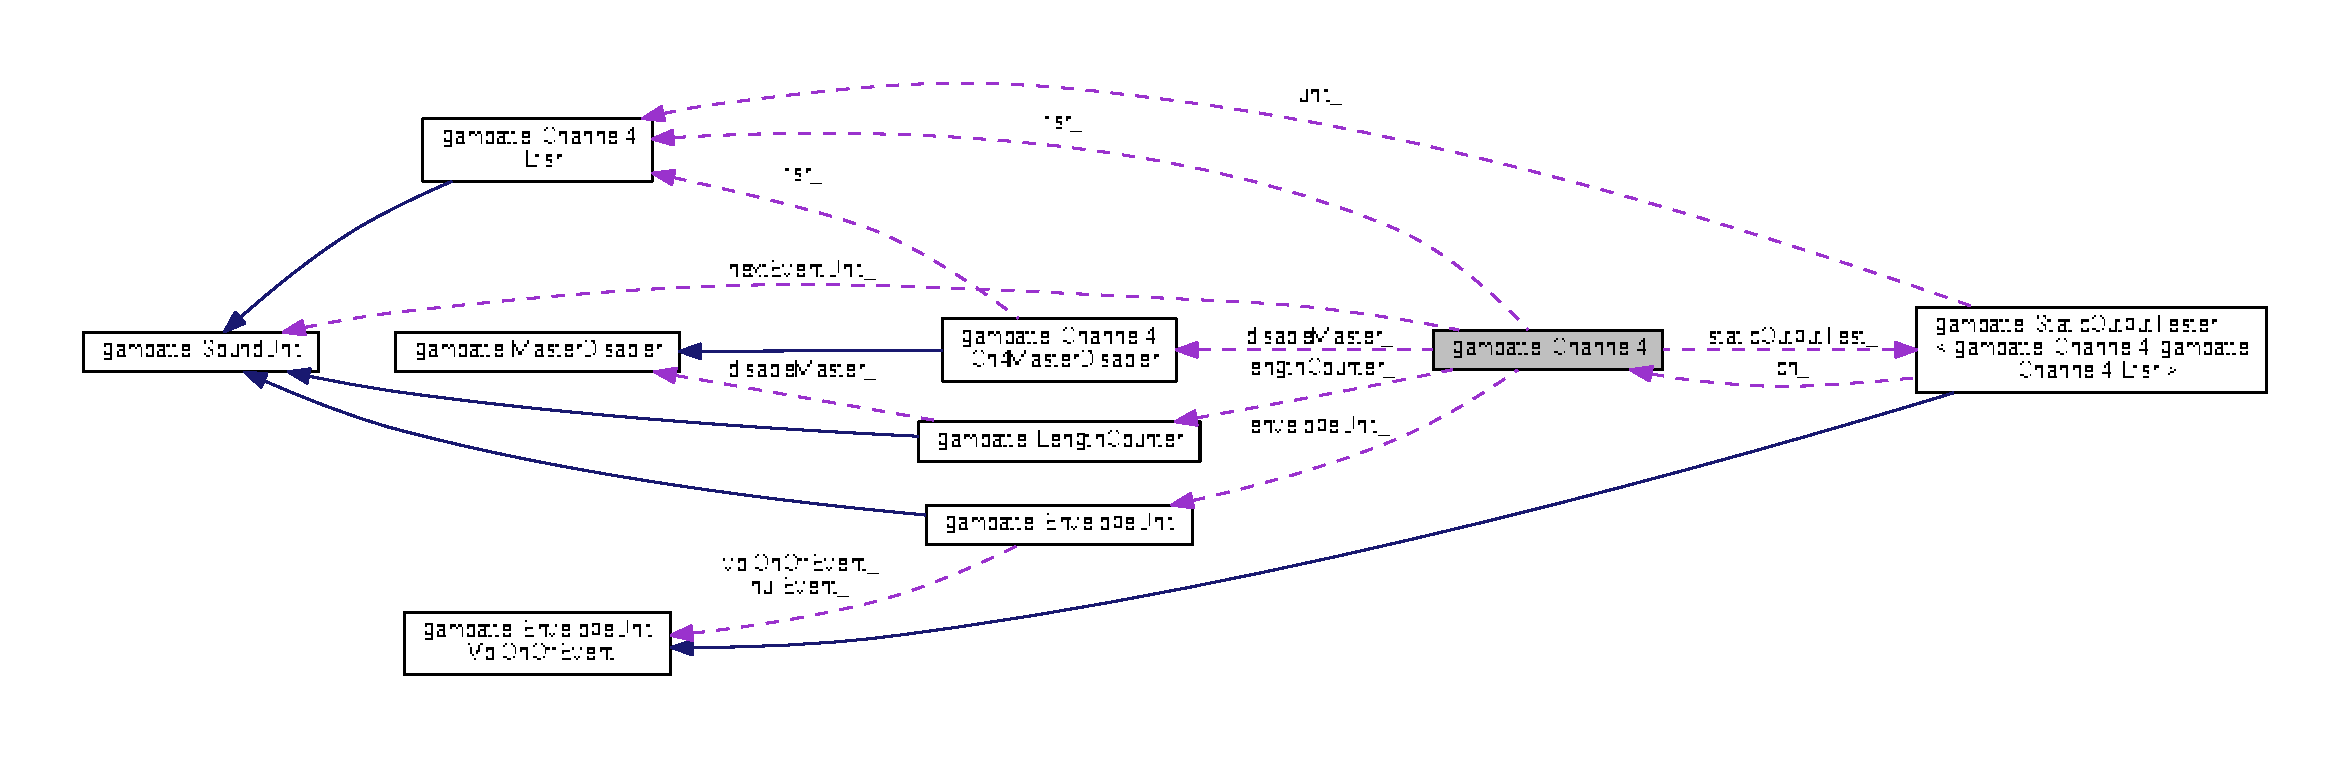
\includegraphics[width=350pt]{classgambatte_1_1Channel4__coll__graph}
\end{center}
\end{figure}
\subsection*{Classes}
\begin{DoxyCompactItemize}
\item 
class \hyperlink{classgambatte_1_1Channel4_1_1Ch4MasterDisabler}{Ch4\+Master\+Disabler}
\item 
class \hyperlink{classgambatte_1_1Channel4_1_1Lfsr}{Lfsr}
\end{DoxyCompactItemize}
\subsection*{Public Member Functions}
\begin{DoxyCompactItemize}
\item 
\hyperlink{classgambatte_1_1Channel4_a54ef50ebeae47194401f0ef3b9a42779}{Channel4} ()
\item 
void \hyperlink{classgambatte_1_1Channel4_a29c6023cb669f67015be405d9fd11e84}{set\+Nr1} (unsigned data)
\item 
void \hyperlink{classgambatte_1_1Channel4_a7a21ae3524252511625070809422112f}{set\+Nr2} (unsigned data)
\item 
void \hyperlink{classgambatte_1_1Channel4_a4c7beb366f4cd1879fbc3932b83bac1c}{set\+Nr3} (unsigned data)
\item 
void \hyperlink{classgambatte_1_1Channel4_a7c5516829899996fb0413694fb560550}{set\+Nr4} (unsigned data)
\item 
void \hyperlink{classgambatte_1_1Channel4_a795b90550082949eb375a5a242bc6137}{load\+Or\+Save} (\hyperlink{classgambatte_1_1loadsave}{loadsave} \&\hyperlink{ppu_8cpp_a2f2eca6997ee7baf8901725ae074d45b}{state})
\item 
void \hyperlink{classgambatte_1_1Channel4_aed1eb1e4bc6a1fdf30e74de63d03e46c}{set\+So} (unsigned so\+Mask)
\item 
bool \hyperlink{classgambatte_1_1Channel4_a5e0e0a8fd225f1547683f813639f8ec3}{is\+Active} () const
\item 
void \hyperlink{classgambatte_1_1Channel4_acac1c7d6828c6041f3f113275c470fb5}{update} (\hyperlink{namespacegambatte_a0639f09fccfbbd5a8e0796318768e370}{uint\+\_\+least32\+\_\+t} $\ast$\hyperlink{ioapi_8h_a8ad8a13c88886b9f623034ff88570adb}{buf}, unsigned so\+Base\+Vol, unsigned cycles)
\item 
void \hyperlink{classgambatte_1_1Channel4_aa4b407e10ce0514b5d1331655e8835cd}{reset} ()
\item 
void \hyperlink{classgambatte_1_1Channel4_ac7c73d2ecf5f29b8ead9497d593602cb}{init} (bool cgb)
\item 
void \hyperlink{classgambatte_1_1Channel4_a59e6a5fccc0b14b93cf0eceb3ba4087c}{save\+State} (\hyperlink{structgambatte_1_1SaveState}{Save\+State} \&\hyperlink{ppu_8cpp_a2f2eca6997ee7baf8901725ae074d45b}{state})
\item 
void \hyperlink{classgambatte_1_1Channel4_a43adb9436bcdd83fe0c7a607a03bde26}{load\+State} (\hyperlink{structgambatte_1_1SaveState}{Save\+State} const \&\hyperlink{ppu_8cpp_a2f2eca6997ee7baf8901725ae074d45b}{state})
\end{DoxyCompactItemize}
\subsection*{Private Member Functions}
\begin{DoxyCompactItemize}
\item 
void \hyperlink{classgambatte_1_1Channel4_ac2368165993248064ae125cfe2ca91e1}{set\+Event} ()
\end{DoxyCompactItemize}
\subsection*{Private Attributes}
\begin{DoxyCompactItemize}
\item 
\hyperlink{classgambatte_1_1StaticOutputTester}{Static\+Output\+Tester}$<$ \hyperlink{classgambatte_1_1Channel4}{Channel4}, \hyperlink{classgambatte_1_1Channel4_1_1Lfsr}{Lfsr} $>$ \hyperlink{classgambatte_1_1Channel4_a2ae503294dbb4386f217e90bb08aaa6d}{static\+Output\+Test\+\_\+}
\item 
\hyperlink{classgambatte_1_1Channel4_1_1Ch4MasterDisabler}{Ch4\+Master\+Disabler} \hyperlink{classgambatte_1_1Channel4_aeefcab821229da926e19fb11ac2ef458}{disable\+Master\+\_\+}
\item 
\hyperlink{classgambatte_1_1LengthCounter}{Length\+Counter} \hyperlink{classgambatte_1_1Channel4_a4f9c75702f5a400ea6ca17434c6e6b29}{length\+Counter\+\_\+}
\item 
\hyperlink{classgambatte_1_1EnvelopeUnit}{Envelope\+Unit} \hyperlink{classgambatte_1_1Channel4_ae07fccf524b60794a12e5afc0342b94e}{envelope\+Unit\+\_\+}
\item 
\hyperlink{classgambatte_1_1Channel4_1_1Lfsr}{Lfsr} \hyperlink{classgambatte_1_1Channel4_a5493adf86be0159f03099f9e8075cd39}{lfsr\+\_\+}
\item 
\hyperlink{classgambatte_1_1SoundUnit}{Sound\+Unit} $\ast$ \hyperlink{classgambatte_1_1Channel4_ab444e6e073b5dd7a2759d50d994f281d}{next\+Event\+Unit\+\_\+}
\item 
unsigned \hyperlink{classgambatte_1_1Channel4_acd27b1580124db2ae0d5d9d5a2a37119}{cycle\+Counter\+\_\+}
\item 
unsigned \hyperlink{classgambatte_1_1Channel4_aee75980e238dc250c990699d992b7416}{so\+Mask\+\_\+}
\item 
unsigned \hyperlink{classgambatte_1_1Channel4_a9ec39dc02e8e49b3fa5814948a165012}{prev\+Out\+\_\+}
\item 
unsigned char \hyperlink{classgambatte_1_1Channel4_af5b498521db67593f428c2bec73bc071}{nr4\+\_\+}
\item 
bool \hyperlink{classgambatte_1_1Channel4_a25e0e535a19cce5e84f1c3a861a0bce3}{master\+\_\+}
\end{DoxyCompactItemize}
\subsection*{Friends}
\begin{DoxyCompactItemize}
\item 
class \hyperlink{classgambatte_1_1Channel4_acf79fbb08fa62daf487648e7d1d91458}{Static\+Output\+Tester$<$ Channel4, Lfsr $>$}
\end{DoxyCompactItemize}


\subsection{Constructor \& Destructor Documentation}
\mbox{\Hypertarget{classgambatte_1_1Channel4_a54ef50ebeae47194401f0ef3b9a42779}\label{classgambatte_1_1Channel4_a54ef50ebeae47194401f0ef3b9a42779}} 
\index{gambatte\+::\+Channel4@{gambatte\+::\+Channel4}!Channel4@{Channel4}}
\index{Channel4@{Channel4}!gambatte\+::\+Channel4@{gambatte\+::\+Channel4}}
\subsubsection{\texorpdfstring{Channel4()}{Channel4()}}
{\footnotesize\ttfamily gambatte\+::\+Channel4\+::\+Channel4 (\begin{DoxyParamCaption}{ }\end{DoxyParamCaption})}



\subsection{Member Function Documentation}
\mbox{\Hypertarget{classgambatte_1_1Channel4_ac7c73d2ecf5f29b8ead9497d593602cb}\label{classgambatte_1_1Channel4_ac7c73d2ecf5f29b8ead9497d593602cb}} 
\index{gambatte\+::\+Channel4@{gambatte\+::\+Channel4}!init@{init}}
\index{init@{init}!gambatte\+::\+Channel4@{gambatte\+::\+Channel4}}
\subsubsection{\texorpdfstring{init()}{init()}}
{\footnotesize\ttfamily void gambatte\+::\+Channel4\+::init (\begin{DoxyParamCaption}\item[{bool}]{cgb }\end{DoxyParamCaption})}

\mbox{\Hypertarget{classgambatte_1_1Channel4_a5e0e0a8fd225f1547683f813639f8ec3}\label{classgambatte_1_1Channel4_a5e0e0a8fd225f1547683f813639f8ec3}} 
\index{gambatte\+::\+Channel4@{gambatte\+::\+Channel4}!is\+Active@{is\+Active}}
\index{is\+Active@{is\+Active}!gambatte\+::\+Channel4@{gambatte\+::\+Channel4}}
\subsubsection{\texorpdfstring{is\+Active()}{isActive()}}
{\footnotesize\ttfamily bool gambatte\+::\+Channel4\+::is\+Active (\begin{DoxyParamCaption}{ }\end{DoxyParamCaption}) const\hspace{0.3cm}{\ttfamily [inline]}}

\mbox{\Hypertarget{classgambatte_1_1Channel4_a795b90550082949eb375a5a242bc6137}\label{classgambatte_1_1Channel4_a795b90550082949eb375a5a242bc6137}} 
\index{gambatte\+::\+Channel4@{gambatte\+::\+Channel4}!load\+Or\+Save@{load\+Or\+Save}}
\index{load\+Or\+Save@{load\+Or\+Save}!gambatte\+::\+Channel4@{gambatte\+::\+Channel4}}
\subsubsection{\texorpdfstring{load\+Or\+Save()}{loadOrSave()}}
{\footnotesize\ttfamily void gambatte\+::\+Channel4\+::load\+Or\+Save (\begin{DoxyParamCaption}\item[{\hyperlink{classgambatte_1_1loadsave}{loadsave} \&}]{state }\end{DoxyParamCaption})}

\mbox{\Hypertarget{classgambatte_1_1Channel4_a43adb9436bcdd83fe0c7a607a03bde26}\label{classgambatte_1_1Channel4_a43adb9436bcdd83fe0c7a607a03bde26}} 
\index{gambatte\+::\+Channel4@{gambatte\+::\+Channel4}!load\+State@{load\+State}}
\index{load\+State@{load\+State}!gambatte\+::\+Channel4@{gambatte\+::\+Channel4}}
\subsubsection{\texorpdfstring{load\+State()}{loadState()}}
{\footnotesize\ttfamily void gambatte\+::\+Channel4\+::load\+State (\begin{DoxyParamCaption}\item[{\hyperlink{structgambatte_1_1SaveState}{Save\+State} const \&}]{state }\end{DoxyParamCaption})}

\mbox{\Hypertarget{classgambatte_1_1Channel4_aa4b407e10ce0514b5d1331655e8835cd}\label{classgambatte_1_1Channel4_aa4b407e10ce0514b5d1331655e8835cd}} 
\index{gambatte\+::\+Channel4@{gambatte\+::\+Channel4}!reset@{reset}}
\index{reset@{reset}!gambatte\+::\+Channel4@{gambatte\+::\+Channel4}}
\subsubsection{\texorpdfstring{reset()}{reset()}}
{\footnotesize\ttfamily void gambatte\+::\+Channel4\+::reset (\begin{DoxyParamCaption}{ }\end{DoxyParamCaption})}

\mbox{\Hypertarget{classgambatte_1_1Channel4_a59e6a5fccc0b14b93cf0eceb3ba4087c}\label{classgambatte_1_1Channel4_a59e6a5fccc0b14b93cf0eceb3ba4087c}} 
\index{gambatte\+::\+Channel4@{gambatte\+::\+Channel4}!save\+State@{save\+State}}
\index{save\+State@{save\+State}!gambatte\+::\+Channel4@{gambatte\+::\+Channel4}}
\subsubsection{\texorpdfstring{save\+State()}{saveState()}}
{\footnotesize\ttfamily void gambatte\+::\+Channel4\+::save\+State (\begin{DoxyParamCaption}\item[{\hyperlink{structgambatte_1_1SaveState}{Save\+State} \&}]{state }\end{DoxyParamCaption})}

\mbox{\Hypertarget{classgambatte_1_1Channel4_ac2368165993248064ae125cfe2ca91e1}\label{classgambatte_1_1Channel4_ac2368165993248064ae125cfe2ca91e1}} 
\index{gambatte\+::\+Channel4@{gambatte\+::\+Channel4}!set\+Event@{set\+Event}}
\index{set\+Event@{set\+Event}!gambatte\+::\+Channel4@{gambatte\+::\+Channel4}}
\subsubsection{\texorpdfstring{set\+Event()}{setEvent()}}
{\footnotesize\ttfamily void gambatte\+::\+Channel4\+::set\+Event (\begin{DoxyParamCaption}{ }\end{DoxyParamCaption})\hspace{0.3cm}{\ttfamily [private]}}

\mbox{\Hypertarget{classgambatte_1_1Channel4_a29c6023cb669f67015be405d9fd11e84}\label{classgambatte_1_1Channel4_a29c6023cb669f67015be405d9fd11e84}} 
\index{gambatte\+::\+Channel4@{gambatte\+::\+Channel4}!set\+Nr1@{set\+Nr1}}
\index{set\+Nr1@{set\+Nr1}!gambatte\+::\+Channel4@{gambatte\+::\+Channel4}}
\subsubsection{\texorpdfstring{set\+Nr1()}{setNr1()}}
{\footnotesize\ttfamily void gambatte\+::\+Channel4\+::set\+Nr1 (\begin{DoxyParamCaption}\item[{unsigned}]{data }\end{DoxyParamCaption})}

\mbox{\Hypertarget{classgambatte_1_1Channel4_a7a21ae3524252511625070809422112f}\label{classgambatte_1_1Channel4_a7a21ae3524252511625070809422112f}} 
\index{gambatte\+::\+Channel4@{gambatte\+::\+Channel4}!set\+Nr2@{set\+Nr2}}
\index{set\+Nr2@{set\+Nr2}!gambatte\+::\+Channel4@{gambatte\+::\+Channel4}}
\subsubsection{\texorpdfstring{set\+Nr2()}{setNr2()}}
{\footnotesize\ttfamily void gambatte\+::\+Channel4\+::set\+Nr2 (\begin{DoxyParamCaption}\item[{unsigned}]{data }\end{DoxyParamCaption})}

\mbox{\Hypertarget{classgambatte_1_1Channel4_a4c7beb366f4cd1879fbc3932b83bac1c}\label{classgambatte_1_1Channel4_a4c7beb366f4cd1879fbc3932b83bac1c}} 
\index{gambatte\+::\+Channel4@{gambatte\+::\+Channel4}!set\+Nr3@{set\+Nr3}}
\index{set\+Nr3@{set\+Nr3}!gambatte\+::\+Channel4@{gambatte\+::\+Channel4}}
\subsubsection{\texorpdfstring{set\+Nr3()}{setNr3()}}
{\footnotesize\ttfamily void gambatte\+::\+Channel4\+::set\+Nr3 (\begin{DoxyParamCaption}\item[{unsigned}]{data }\end{DoxyParamCaption})\hspace{0.3cm}{\ttfamily [inline]}}

\mbox{\Hypertarget{classgambatte_1_1Channel4_a7c5516829899996fb0413694fb560550}\label{classgambatte_1_1Channel4_a7c5516829899996fb0413694fb560550}} 
\index{gambatte\+::\+Channel4@{gambatte\+::\+Channel4}!set\+Nr4@{set\+Nr4}}
\index{set\+Nr4@{set\+Nr4}!gambatte\+::\+Channel4@{gambatte\+::\+Channel4}}
\subsubsection{\texorpdfstring{set\+Nr4()}{setNr4()}}
{\footnotesize\ttfamily void gambatte\+::\+Channel4\+::set\+Nr4 (\begin{DoxyParamCaption}\item[{unsigned}]{data }\end{DoxyParamCaption})}

\mbox{\Hypertarget{classgambatte_1_1Channel4_aed1eb1e4bc6a1fdf30e74de63d03e46c}\label{classgambatte_1_1Channel4_aed1eb1e4bc6a1fdf30e74de63d03e46c}} 
\index{gambatte\+::\+Channel4@{gambatte\+::\+Channel4}!set\+So@{set\+So}}
\index{set\+So@{set\+So}!gambatte\+::\+Channel4@{gambatte\+::\+Channel4}}
\subsubsection{\texorpdfstring{set\+So()}{setSo()}}
{\footnotesize\ttfamily void gambatte\+::\+Channel4\+::set\+So (\begin{DoxyParamCaption}\item[{unsigned}]{so\+Mask }\end{DoxyParamCaption})}

\mbox{\Hypertarget{classgambatte_1_1Channel4_acac1c7d6828c6041f3f113275c470fb5}\label{classgambatte_1_1Channel4_acac1c7d6828c6041f3f113275c470fb5}} 
\index{gambatte\+::\+Channel4@{gambatte\+::\+Channel4}!update@{update}}
\index{update@{update}!gambatte\+::\+Channel4@{gambatte\+::\+Channel4}}
\subsubsection{\texorpdfstring{update()}{update()}}
{\footnotesize\ttfamily void gambatte\+::\+Channel4\+::update (\begin{DoxyParamCaption}\item[{\hyperlink{namespacegambatte_a0639f09fccfbbd5a8e0796318768e370}{uint\+\_\+least32\+\_\+t} $\ast$}]{buf,  }\item[{unsigned}]{so\+Base\+Vol,  }\item[{unsigned}]{cycles }\end{DoxyParamCaption})}



\subsection{Friends And Related Function Documentation}
\mbox{\Hypertarget{classgambatte_1_1Channel4_acf79fbb08fa62daf487648e7d1d91458}\label{classgambatte_1_1Channel4_acf79fbb08fa62daf487648e7d1d91458}} 
\index{gambatte\+::\+Channel4@{gambatte\+::\+Channel4}!Static\+Output\+Tester$<$ Channel4, Lfsr $>$@{Static\+Output\+Tester$<$ Channel4, Lfsr $>$}}
\index{Static\+Output\+Tester$<$ Channel4, Lfsr $>$@{Static\+Output\+Tester$<$ Channel4, Lfsr $>$}!gambatte\+::\+Channel4@{gambatte\+::\+Channel4}}
\subsubsection{\texorpdfstring{Static\+Output\+Tester$<$ Channel4, Lfsr $>$}{StaticOutputTester< Channel4, Lfsr >}}
{\footnotesize\ttfamily friend class \hyperlink{classgambatte_1_1StaticOutputTester}{Static\+Output\+Tester}$<$ \hyperlink{classgambatte_1_1Channel4}{Channel4}, \hyperlink{classgambatte_1_1Channel4_1_1Lfsr}{Lfsr} $>$\hspace{0.3cm}{\ttfamily [friend]}}



\subsection{Member Data Documentation}
\mbox{\Hypertarget{classgambatte_1_1Channel4_acd27b1580124db2ae0d5d9d5a2a37119}\label{classgambatte_1_1Channel4_acd27b1580124db2ae0d5d9d5a2a37119}} 
\index{gambatte\+::\+Channel4@{gambatte\+::\+Channel4}!cycle\+Counter\+\_\+@{cycle\+Counter\+\_\+}}
\index{cycle\+Counter\+\_\+@{cycle\+Counter\+\_\+}!gambatte\+::\+Channel4@{gambatte\+::\+Channel4}}
\subsubsection{\texorpdfstring{cycle\+Counter\+\_\+}{cycleCounter\_}}
{\footnotesize\ttfamily unsigned gambatte\+::\+Channel4\+::cycle\+Counter\+\_\+\hspace{0.3cm}{\ttfamily [private]}}

\mbox{\Hypertarget{classgambatte_1_1Channel4_aeefcab821229da926e19fb11ac2ef458}\label{classgambatte_1_1Channel4_aeefcab821229da926e19fb11ac2ef458}} 
\index{gambatte\+::\+Channel4@{gambatte\+::\+Channel4}!disable\+Master\+\_\+@{disable\+Master\+\_\+}}
\index{disable\+Master\+\_\+@{disable\+Master\+\_\+}!gambatte\+::\+Channel4@{gambatte\+::\+Channel4}}
\subsubsection{\texorpdfstring{disable\+Master\+\_\+}{disableMaster\_}}
{\footnotesize\ttfamily \hyperlink{classgambatte_1_1Channel4_1_1Ch4MasterDisabler}{Ch4\+Master\+Disabler} gambatte\+::\+Channel4\+::disable\+Master\+\_\+\hspace{0.3cm}{\ttfamily [private]}}

\mbox{\Hypertarget{classgambatte_1_1Channel4_ae07fccf524b60794a12e5afc0342b94e}\label{classgambatte_1_1Channel4_ae07fccf524b60794a12e5afc0342b94e}} 
\index{gambatte\+::\+Channel4@{gambatte\+::\+Channel4}!envelope\+Unit\+\_\+@{envelope\+Unit\+\_\+}}
\index{envelope\+Unit\+\_\+@{envelope\+Unit\+\_\+}!gambatte\+::\+Channel4@{gambatte\+::\+Channel4}}
\subsubsection{\texorpdfstring{envelope\+Unit\+\_\+}{envelopeUnit\_}}
{\footnotesize\ttfamily \hyperlink{classgambatte_1_1EnvelopeUnit}{Envelope\+Unit} gambatte\+::\+Channel4\+::envelope\+Unit\+\_\+\hspace{0.3cm}{\ttfamily [private]}}

\mbox{\Hypertarget{classgambatte_1_1Channel4_a4f9c75702f5a400ea6ca17434c6e6b29}\label{classgambatte_1_1Channel4_a4f9c75702f5a400ea6ca17434c6e6b29}} 
\index{gambatte\+::\+Channel4@{gambatte\+::\+Channel4}!length\+Counter\+\_\+@{length\+Counter\+\_\+}}
\index{length\+Counter\+\_\+@{length\+Counter\+\_\+}!gambatte\+::\+Channel4@{gambatte\+::\+Channel4}}
\subsubsection{\texorpdfstring{length\+Counter\+\_\+}{lengthCounter\_}}
{\footnotesize\ttfamily \hyperlink{classgambatte_1_1LengthCounter}{Length\+Counter} gambatte\+::\+Channel4\+::length\+Counter\+\_\+\hspace{0.3cm}{\ttfamily [private]}}

\mbox{\Hypertarget{classgambatte_1_1Channel4_a5493adf86be0159f03099f9e8075cd39}\label{classgambatte_1_1Channel4_a5493adf86be0159f03099f9e8075cd39}} 
\index{gambatte\+::\+Channel4@{gambatte\+::\+Channel4}!lfsr\+\_\+@{lfsr\+\_\+}}
\index{lfsr\+\_\+@{lfsr\+\_\+}!gambatte\+::\+Channel4@{gambatte\+::\+Channel4}}
\subsubsection{\texorpdfstring{lfsr\+\_\+}{lfsr\_}}
{\footnotesize\ttfamily \hyperlink{classgambatte_1_1Channel4_1_1Lfsr}{Lfsr} gambatte\+::\+Channel4\+::lfsr\+\_\+\hspace{0.3cm}{\ttfamily [private]}}

\mbox{\Hypertarget{classgambatte_1_1Channel4_a25e0e535a19cce5e84f1c3a861a0bce3}\label{classgambatte_1_1Channel4_a25e0e535a19cce5e84f1c3a861a0bce3}} 
\index{gambatte\+::\+Channel4@{gambatte\+::\+Channel4}!master\+\_\+@{master\+\_\+}}
\index{master\+\_\+@{master\+\_\+}!gambatte\+::\+Channel4@{gambatte\+::\+Channel4}}
\subsubsection{\texorpdfstring{master\+\_\+}{master\_}}
{\footnotesize\ttfamily bool gambatte\+::\+Channel4\+::master\+\_\+\hspace{0.3cm}{\ttfamily [private]}}

\mbox{\Hypertarget{classgambatte_1_1Channel4_ab444e6e073b5dd7a2759d50d994f281d}\label{classgambatte_1_1Channel4_ab444e6e073b5dd7a2759d50d994f281d}} 
\index{gambatte\+::\+Channel4@{gambatte\+::\+Channel4}!next\+Event\+Unit\+\_\+@{next\+Event\+Unit\+\_\+}}
\index{next\+Event\+Unit\+\_\+@{next\+Event\+Unit\+\_\+}!gambatte\+::\+Channel4@{gambatte\+::\+Channel4}}
\subsubsection{\texorpdfstring{next\+Event\+Unit\+\_\+}{nextEventUnit\_}}
{\footnotesize\ttfamily \hyperlink{classgambatte_1_1SoundUnit}{Sound\+Unit}$\ast$ gambatte\+::\+Channel4\+::next\+Event\+Unit\+\_\+\hspace{0.3cm}{\ttfamily [private]}}

\mbox{\Hypertarget{classgambatte_1_1Channel4_af5b498521db67593f428c2bec73bc071}\label{classgambatte_1_1Channel4_af5b498521db67593f428c2bec73bc071}} 
\index{gambatte\+::\+Channel4@{gambatte\+::\+Channel4}!nr4\+\_\+@{nr4\+\_\+}}
\index{nr4\+\_\+@{nr4\+\_\+}!gambatte\+::\+Channel4@{gambatte\+::\+Channel4}}
\subsubsection{\texorpdfstring{nr4\+\_\+}{nr4\_}}
{\footnotesize\ttfamily unsigned char gambatte\+::\+Channel4\+::nr4\+\_\+\hspace{0.3cm}{\ttfamily [private]}}

\mbox{\Hypertarget{classgambatte_1_1Channel4_a9ec39dc02e8e49b3fa5814948a165012}\label{classgambatte_1_1Channel4_a9ec39dc02e8e49b3fa5814948a165012}} 
\index{gambatte\+::\+Channel4@{gambatte\+::\+Channel4}!prev\+Out\+\_\+@{prev\+Out\+\_\+}}
\index{prev\+Out\+\_\+@{prev\+Out\+\_\+}!gambatte\+::\+Channel4@{gambatte\+::\+Channel4}}
\subsubsection{\texorpdfstring{prev\+Out\+\_\+}{prevOut\_}}
{\footnotesize\ttfamily unsigned gambatte\+::\+Channel4\+::prev\+Out\+\_\+\hspace{0.3cm}{\ttfamily [private]}}

\mbox{\Hypertarget{classgambatte_1_1Channel4_aee75980e238dc250c990699d992b7416}\label{classgambatte_1_1Channel4_aee75980e238dc250c990699d992b7416}} 
\index{gambatte\+::\+Channel4@{gambatte\+::\+Channel4}!so\+Mask\+\_\+@{so\+Mask\+\_\+}}
\index{so\+Mask\+\_\+@{so\+Mask\+\_\+}!gambatte\+::\+Channel4@{gambatte\+::\+Channel4}}
\subsubsection{\texorpdfstring{so\+Mask\+\_\+}{soMask\_}}
{\footnotesize\ttfamily unsigned gambatte\+::\+Channel4\+::so\+Mask\+\_\+\hspace{0.3cm}{\ttfamily [private]}}

\mbox{\Hypertarget{classgambatte_1_1Channel4_a2ae503294dbb4386f217e90bb08aaa6d}\label{classgambatte_1_1Channel4_a2ae503294dbb4386f217e90bb08aaa6d}} 
\index{gambatte\+::\+Channel4@{gambatte\+::\+Channel4}!static\+Output\+Test\+\_\+@{static\+Output\+Test\+\_\+}}
\index{static\+Output\+Test\+\_\+@{static\+Output\+Test\+\_\+}!gambatte\+::\+Channel4@{gambatte\+::\+Channel4}}
\subsubsection{\texorpdfstring{static\+Output\+Test\+\_\+}{staticOutputTest\_}}
{\footnotesize\ttfamily \hyperlink{classgambatte_1_1StaticOutputTester}{Static\+Output\+Tester}$<$\hyperlink{classgambatte_1_1Channel4}{Channel4}, \hyperlink{classgambatte_1_1Channel4_1_1Lfsr}{Lfsr}$>$ gambatte\+::\+Channel4\+::static\+Output\+Test\+\_\+\hspace{0.3cm}{\ttfamily [private]}}



The documentation for this class was generated from the following files\+:\begin{DoxyCompactItemize}
\item 
src/sound/\hyperlink{channel4_8h}{channel4.\+h}\item 
src/sound/\hyperlink{channel4_8cpp}{channel4.\+cpp}\end{DoxyCompactItemize}

\hypertarget{structgambatte_1_1SaveState_1_1CPU}{}\section{gambatte\+:\+:Save\+State\+:\+:C\+PU Struct Reference}
\label{structgambatte_1_1SaveState_1_1CPU}\index{gambatte\+::\+Save\+State\+::\+C\+PU@{gambatte\+::\+Save\+State\+::\+C\+PU}}


{\ttfamily \#include $<$savestate.\+h$>$}

\subsection*{Public Attributes}
\begin{DoxyCompactItemize}
\item 
unsigned \hyperlink{structgambatte_1_1SaveState_1_1CPU_ae90b1140ae3783f2a2f231392cc69252}{cycle\+Counter}
\item 
unsigned short \hyperlink{structgambatte_1_1SaveState_1_1CPU_af7aecc14631c530186955584cd335862}{pc}
\item 
unsigned short \hyperlink{structgambatte_1_1SaveState_1_1CPU_a6f044fbd101e0bfa5e8762f134897c4b}{sp}
\item 
unsigned char \hyperlink{structgambatte_1_1SaveState_1_1CPU_abdaf265b0edd02408180873a8f3b386c}{a}
\item 
unsigned char \hyperlink{structgambatte_1_1SaveState_1_1CPU_a79056f7d29fe5033059c4fe4b03a6392}{b}
\item 
unsigned char \hyperlink{structgambatte_1_1SaveState_1_1CPU_a8ca2a8ea344927ecb73f3afddd1b28fd}{c}
\item 
unsigned char \hyperlink{structgambatte_1_1SaveState_1_1CPU_a220b57e70d3c110e0157985ce5a77d5d}{d}
\item 
unsigned char \hyperlink{structgambatte_1_1SaveState_1_1CPU_ac2df8c0e7e1f487689a83c930c698416}{e}
\item 
unsigned char \hyperlink{structgambatte_1_1SaveState_1_1CPU_ab7f3b5513b72b3c21c0c98cef694f7c2}{f}
\item 
unsigned char \hyperlink{structgambatte_1_1SaveState_1_1CPU_ad2e3e9aa15bbf00ea6454066bf898f14}{h}
\item 
unsigned char \hyperlink{structgambatte_1_1SaveState_1_1CPU_a1be44c38f3b0a4440fba7b1e9e3240a3}{l}
\item 
bool \hyperlink{structgambatte_1_1SaveState_1_1CPU_abc5cc42019adeb561c76c4ef69787c8f}{skip}
\end{DoxyCompactItemize}


\subsection{Member Data Documentation}
\mbox{\Hypertarget{structgambatte_1_1SaveState_1_1CPU_abdaf265b0edd02408180873a8f3b386c}\label{structgambatte_1_1SaveState_1_1CPU_abdaf265b0edd02408180873a8f3b386c}} 
\index{gambatte\+::\+Save\+State\+::\+C\+PU@{gambatte\+::\+Save\+State\+::\+C\+PU}!a@{a}}
\index{a@{a}!gambatte\+::\+Save\+State\+::\+C\+PU@{gambatte\+::\+Save\+State\+::\+C\+PU}}
\subsubsection{\texorpdfstring{a}{a}}
{\footnotesize\ttfamily unsigned char gambatte\+::\+Save\+State\+::\+C\+P\+U\+::a}

\mbox{\Hypertarget{structgambatte_1_1SaveState_1_1CPU_a79056f7d29fe5033059c4fe4b03a6392}\label{structgambatte_1_1SaveState_1_1CPU_a79056f7d29fe5033059c4fe4b03a6392}} 
\index{gambatte\+::\+Save\+State\+::\+C\+PU@{gambatte\+::\+Save\+State\+::\+C\+PU}!b@{b}}
\index{b@{b}!gambatte\+::\+Save\+State\+::\+C\+PU@{gambatte\+::\+Save\+State\+::\+C\+PU}}
\subsubsection{\texorpdfstring{b}{b}}
{\footnotesize\ttfamily unsigned char gambatte\+::\+Save\+State\+::\+C\+P\+U\+::b}

\mbox{\Hypertarget{structgambatte_1_1SaveState_1_1CPU_a8ca2a8ea344927ecb73f3afddd1b28fd}\label{structgambatte_1_1SaveState_1_1CPU_a8ca2a8ea344927ecb73f3afddd1b28fd}} 
\index{gambatte\+::\+Save\+State\+::\+C\+PU@{gambatte\+::\+Save\+State\+::\+C\+PU}!c@{c}}
\index{c@{c}!gambatte\+::\+Save\+State\+::\+C\+PU@{gambatte\+::\+Save\+State\+::\+C\+PU}}
\subsubsection{\texorpdfstring{c}{c}}
{\footnotesize\ttfamily unsigned char gambatte\+::\+Save\+State\+::\+C\+P\+U\+::c}

\mbox{\Hypertarget{structgambatte_1_1SaveState_1_1CPU_ae90b1140ae3783f2a2f231392cc69252}\label{structgambatte_1_1SaveState_1_1CPU_ae90b1140ae3783f2a2f231392cc69252}} 
\index{gambatte\+::\+Save\+State\+::\+C\+PU@{gambatte\+::\+Save\+State\+::\+C\+PU}!cycle\+Counter@{cycle\+Counter}}
\index{cycle\+Counter@{cycle\+Counter}!gambatte\+::\+Save\+State\+::\+C\+PU@{gambatte\+::\+Save\+State\+::\+C\+PU}}
\subsubsection{\texorpdfstring{cycle\+Counter}{cycleCounter}}
{\footnotesize\ttfamily unsigned gambatte\+::\+Save\+State\+::\+C\+P\+U\+::cycle\+Counter}

\mbox{\Hypertarget{structgambatte_1_1SaveState_1_1CPU_a220b57e70d3c110e0157985ce5a77d5d}\label{structgambatte_1_1SaveState_1_1CPU_a220b57e70d3c110e0157985ce5a77d5d}} 
\index{gambatte\+::\+Save\+State\+::\+C\+PU@{gambatte\+::\+Save\+State\+::\+C\+PU}!d@{d}}
\index{d@{d}!gambatte\+::\+Save\+State\+::\+C\+PU@{gambatte\+::\+Save\+State\+::\+C\+PU}}
\subsubsection{\texorpdfstring{d}{d}}
{\footnotesize\ttfamily unsigned char gambatte\+::\+Save\+State\+::\+C\+P\+U\+::d}

\mbox{\Hypertarget{structgambatte_1_1SaveState_1_1CPU_ac2df8c0e7e1f487689a83c930c698416}\label{structgambatte_1_1SaveState_1_1CPU_ac2df8c0e7e1f487689a83c930c698416}} 
\index{gambatte\+::\+Save\+State\+::\+C\+PU@{gambatte\+::\+Save\+State\+::\+C\+PU}!e@{e}}
\index{e@{e}!gambatte\+::\+Save\+State\+::\+C\+PU@{gambatte\+::\+Save\+State\+::\+C\+PU}}
\subsubsection{\texorpdfstring{e}{e}}
{\footnotesize\ttfamily unsigned char gambatte\+::\+Save\+State\+::\+C\+P\+U\+::e}

\mbox{\Hypertarget{structgambatte_1_1SaveState_1_1CPU_ab7f3b5513b72b3c21c0c98cef694f7c2}\label{structgambatte_1_1SaveState_1_1CPU_ab7f3b5513b72b3c21c0c98cef694f7c2}} 
\index{gambatte\+::\+Save\+State\+::\+C\+PU@{gambatte\+::\+Save\+State\+::\+C\+PU}!f@{f}}
\index{f@{f}!gambatte\+::\+Save\+State\+::\+C\+PU@{gambatte\+::\+Save\+State\+::\+C\+PU}}
\subsubsection{\texorpdfstring{f}{f}}
{\footnotesize\ttfamily unsigned char gambatte\+::\+Save\+State\+::\+C\+P\+U\+::f}

\mbox{\Hypertarget{structgambatte_1_1SaveState_1_1CPU_ad2e3e9aa15bbf00ea6454066bf898f14}\label{structgambatte_1_1SaveState_1_1CPU_ad2e3e9aa15bbf00ea6454066bf898f14}} 
\index{gambatte\+::\+Save\+State\+::\+C\+PU@{gambatte\+::\+Save\+State\+::\+C\+PU}!h@{h}}
\index{h@{h}!gambatte\+::\+Save\+State\+::\+C\+PU@{gambatte\+::\+Save\+State\+::\+C\+PU}}
\subsubsection{\texorpdfstring{h}{h}}
{\footnotesize\ttfamily unsigned char gambatte\+::\+Save\+State\+::\+C\+P\+U\+::h}

\mbox{\Hypertarget{structgambatte_1_1SaveState_1_1CPU_a1be44c38f3b0a4440fba7b1e9e3240a3}\label{structgambatte_1_1SaveState_1_1CPU_a1be44c38f3b0a4440fba7b1e9e3240a3}} 
\index{gambatte\+::\+Save\+State\+::\+C\+PU@{gambatte\+::\+Save\+State\+::\+C\+PU}!l@{l}}
\index{l@{l}!gambatte\+::\+Save\+State\+::\+C\+PU@{gambatte\+::\+Save\+State\+::\+C\+PU}}
\subsubsection{\texorpdfstring{l}{l}}
{\footnotesize\ttfamily unsigned char gambatte\+::\+Save\+State\+::\+C\+P\+U\+::l}

\mbox{\Hypertarget{structgambatte_1_1SaveState_1_1CPU_af7aecc14631c530186955584cd335862}\label{structgambatte_1_1SaveState_1_1CPU_af7aecc14631c530186955584cd335862}} 
\index{gambatte\+::\+Save\+State\+::\+C\+PU@{gambatte\+::\+Save\+State\+::\+C\+PU}!pc@{pc}}
\index{pc@{pc}!gambatte\+::\+Save\+State\+::\+C\+PU@{gambatte\+::\+Save\+State\+::\+C\+PU}}
\subsubsection{\texorpdfstring{pc}{pc}}
{\footnotesize\ttfamily unsigned short gambatte\+::\+Save\+State\+::\+C\+P\+U\+::pc}

\mbox{\Hypertarget{structgambatte_1_1SaveState_1_1CPU_abc5cc42019adeb561c76c4ef69787c8f}\label{structgambatte_1_1SaveState_1_1CPU_abc5cc42019adeb561c76c4ef69787c8f}} 
\index{gambatte\+::\+Save\+State\+::\+C\+PU@{gambatte\+::\+Save\+State\+::\+C\+PU}!skip@{skip}}
\index{skip@{skip}!gambatte\+::\+Save\+State\+::\+C\+PU@{gambatte\+::\+Save\+State\+::\+C\+PU}}
\subsubsection{\texorpdfstring{skip}{skip}}
{\footnotesize\ttfamily bool gambatte\+::\+Save\+State\+::\+C\+P\+U\+::skip}

\mbox{\Hypertarget{structgambatte_1_1SaveState_1_1CPU_a6f044fbd101e0bfa5e8762f134897c4b}\label{structgambatte_1_1SaveState_1_1CPU_a6f044fbd101e0bfa5e8762f134897c4b}} 
\index{gambatte\+::\+Save\+State\+::\+C\+PU@{gambatte\+::\+Save\+State\+::\+C\+PU}!sp@{sp}}
\index{sp@{sp}!gambatte\+::\+Save\+State\+::\+C\+PU@{gambatte\+::\+Save\+State\+::\+C\+PU}}
\subsubsection{\texorpdfstring{sp}{sp}}
{\footnotesize\ttfamily unsigned short gambatte\+::\+Save\+State\+::\+C\+P\+U\+::sp}



The documentation for this struct was generated from the following file\+:\begin{DoxyCompactItemize}
\item 
src/\hyperlink{savestate_8h}{savestate.\+h}\end{DoxyCompactItemize}

\hypertarget{classgambatte_1_1CPU}{}\section{gambatte\+:\+:C\+PU Class Reference}
\label{classgambatte_1_1CPU}\index{gambatte\+::\+C\+PU@{gambatte\+::\+C\+PU}}


{\ttfamily \#include $<$cpu.\+h$>$}



Collaboration diagram for gambatte\+:\+:C\+PU\+:
\nopagebreak
\begin{figure}[H]
\begin{center}
\leavevmode
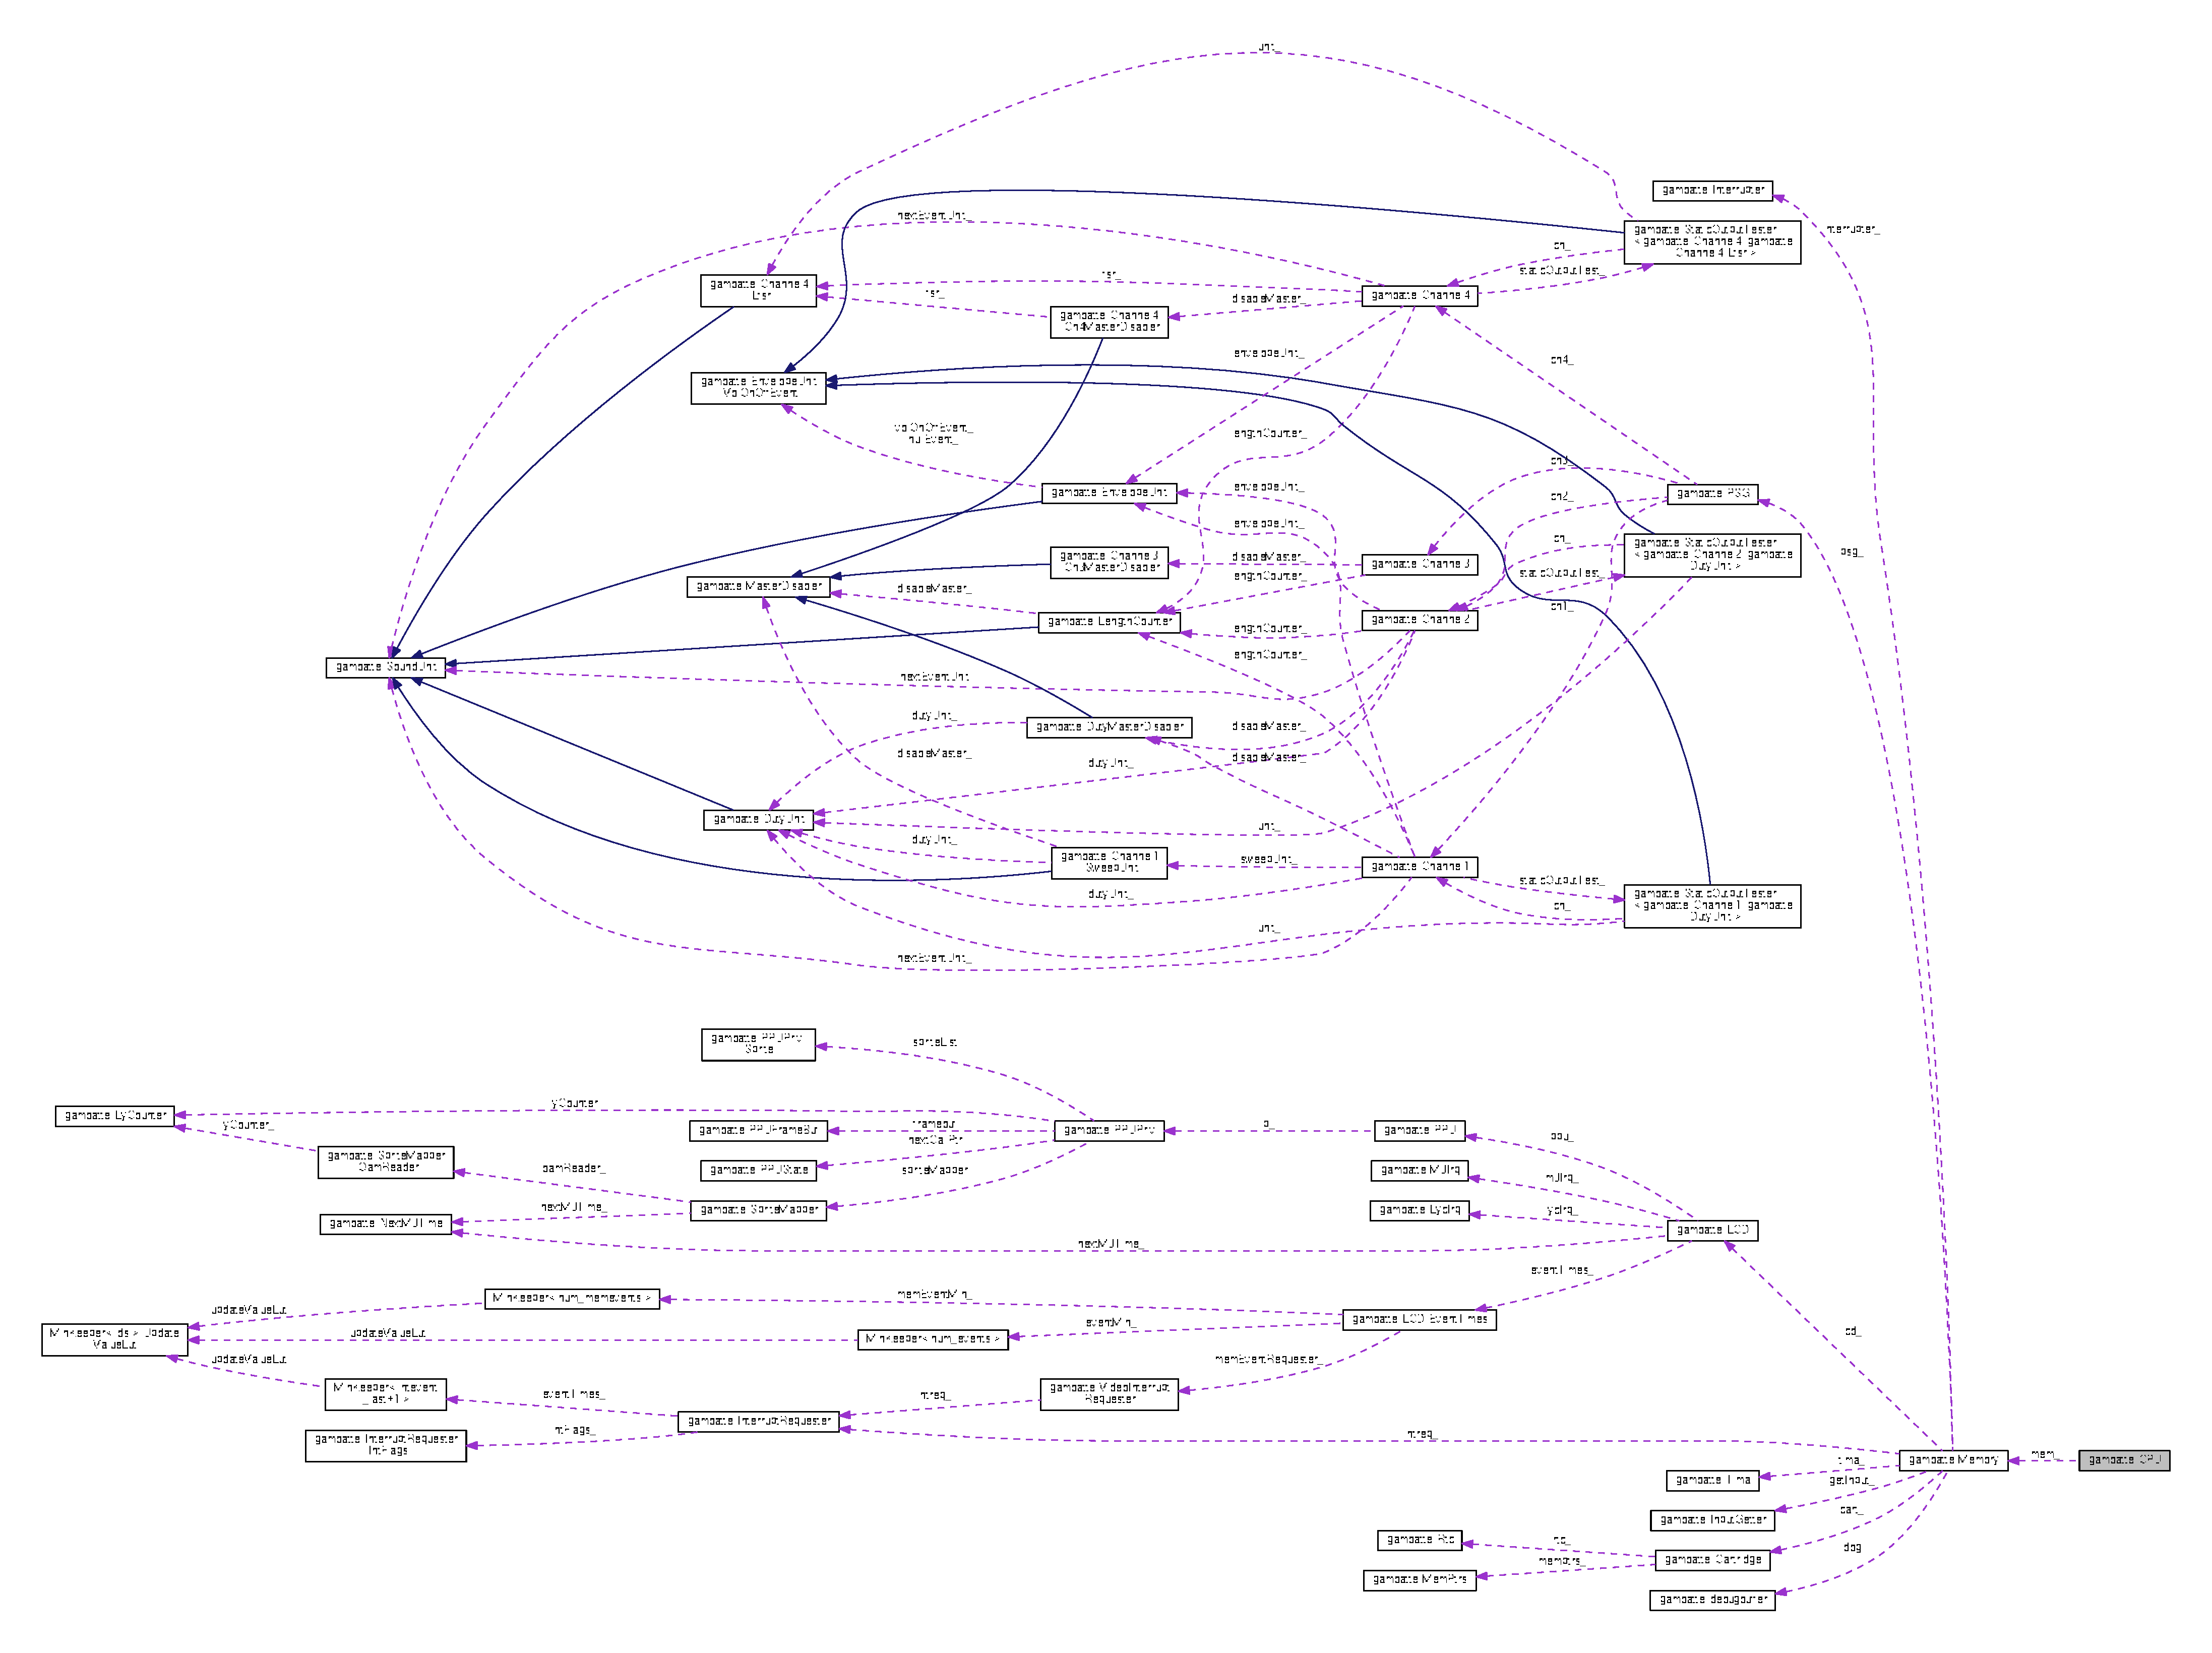
\includegraphics[width=350pt]{classgambatte_1_1CPU__coll__graph}
\end{center}
\end{figure}
\subsection*{Public Member Functions}
\begin{DoxyCompactItemize}
\item 
\hyperlink{classgambatte_1_1CPU_ad2f22383ec6a786778ceb7f834871714}{C\+PU} (time\+\_\+t($\ast$$\ast$\+\_\+get\+Current\+Time)())
\item 
signed \hyperlink{classgambatte_1_1CPU_a578dc9523b8c4fd01b65bac8ab66f3dd}{run\+For} (unsigned cycles)
\item 
void \hyperlink{classgambatte_1_1CPU_ad3536333dfdf2152288d68cd6a0f85f6}{set\+State\+Ptrs} (\hyperlink{structgambatte_1_1SaveState}{Save\+State} \&\hyperlink{ppu_8cpp_a2f2eca6997ee7baf8901725ae074d45b}{state})
\item 
void \hyperlink{classgambatte_1_1CPU_ad18d4bce08093c8c927b68cc2f3339bb}{save\+State} (\hyperlink{structgambatte_1_1SaveState}{Save\+State} \&\hyperlink{ppu_8cpp_a2f2eca6997ee7baf8901725ae074d45b}{state})
\item 
void \hyperlink{classgambatte_1_1CPU_a8e6bb830ddf5af65d28cf3ebfcbddf02}{load\+Or\+Save} (\hyperlink{classgambatte_1_1loadsave}{loadsave} \&\hyperlink{ppu_8cpp_a2f2eca6997ee7baf8901725ae074d45b}{state})
\item 
void \hyperlink{classgambatte_1_1CPU_a92e34858fac97ce269cf72ff114d3e7e}{load\+State} (\hyperlink{structgambatte_1_1SaveState}{Save\+State} const \&\hyperlink{ppu_8cpp_a2f2eca6997ee7baf8901725ae074d45b}{state})
\item 
void \hyperlink{classgambatte_1_1CPU_a8b03ef8733dc634d39998d80c3a75be5}{load\+Savedata} ()
\item 
void \hyperlink{classgambatte_1_1CPU_a4ece2687dec833880531bfaf010e63a6}{save\+Savedata} ()
\item 
void \hyperlink{classgambatte_1_1CPU_a7e12310942f8986295086a9f9c5217ba}{set\+Video\+Buffer} (\hyperlink{namespacegambatte_a0639f09fccfbbd5a8e0796318768e370}{uint\+\_\+least32\+\_\+t} $\ast$video\+Buf, std\+::ptrdiff\+\_\+t pitch)
\item 
void \hyperlink{classgambatte_1_1CPU_a7e9b00d6068a5d4b3b1f3467c6fda8ca}{set\+Input\+Getter} (\hyperlink{classgambatte_1_1InputGetter}{Input\+Getter} $\ast$get\+Input)
\item 
void \hyperlink{classgambatte_1_1CPU_a9c882b42b4e426ae9368a181108f6e92}{set\+Save\+Dir} (std\+::string const \&sdir)
\item 
void \hyperlink{classgambatte_1_1CPU_a3c14c0089808692b7e26033bcc6ad4c9}{set\+\_\+debug\+\_\+buffer} (\hyperlink{structgambatte_1_1debugbuffer}{debugbuffer} \&dbgbuf)
\item 
std\+::string const \hyperlink{classgambatte_1_1CPU_a8eb13a942b95e3b97fe21ac17be82715}{save\+Base\+Path} () const
\item 
void \hyperlink{classgambatte_1_1CPU_a2d58f9e07dde04c2b6000c0c56c05bba}{set\+Osd\+Element} (transfer\+\_\+ptr$<$ \hyperlink{classgambatte_1_1OsdElement}{Osd\+Element} $>$ osd\+Element)
\item 
\hyperlink{namespacegambatte_a42606f494711d2e2870a5f5cdf69e468}{Load\+Res} \hyperlink{classgambatte_1_1CPU_a4aa60bdec265f00ab5f30a2b3498995d}{load} (std\+::string const \&romfile, bool force\+Dmg, bool multicart\+Compat)
\item 
\hyperlink{namespacegambatte_a42606f494711d2e2870a5f5cdf69e468}{Load\+Res} \hyperlink{classgambatte_1_1CPU_a722954e3155c839f2a63532f8c553540}{load} (const unsigned char $\ast$image, size\+\_\+t isize, bool force\+Dmg, bool multicart\+Compat)
\item 
bool \hyperlink{classgambatte_1_1CPU_a20581262d956fd83bc9ff2ec7bf5f8c3}{loaded} () const
\item 
char const  $\ast$ \hyperlink{classgambatte_1_1CPU_a80720dbddb6782b9472186935815d2c3}{rom\+Title} () const
\item 
\hyperlink{classgambatte_1_1PakInfo}{Pak\+Info} const \hyperlink{classgambatte_1_1CPU_afa8d54bb7dbcd31d7b6046c1ba1d4af3}{pak\+Info} (bool multicart\+Compat) const
\item 
void \hyperlink{classgambatte_1_1CPU_ae278996f1f2e328a0340737f856d29c2}{set\+Sound\+Buffer} (\hyperlink{namespacegambatte_a0639f09fccfbbd5a8e0796318768e370}{uint\+\_\+least32\+\_\+t} $\ast$\hyperlink{ioapi_8h_a8ad8a13c88886b9f623034ff88570adb}{buf})
\item 
std\+::size\+\_\+t \hyperlink{classgambatte_1_1CPU_a42bcefacaf365386e39b6c446f1d98c6}{fill\+Sound\+Buffer} ()
\item 
bool \hyperlink{classgambatte_1_1CPU_aca376b5dfd036aaf0f28f92f7ea357ed}{is\+Cgb} () const
\item 
void \hyperlink{classgambatte_1_1CPU_a4453327ee201a535a33ec761d77f686e}{set\+Dmg\+Palette\+Color} (\hyperlink{ioapi_8h_a787fa3cf048117ba7123753c1e74fcd6}{int} pal\+Num, \hyperlink{ioapi_8h_a787fa3cf048117ba7123753c1e74fcd6}{int} color\+Num, \hyperlink{namespacegambatte_a0639f09fccfbbd5a8e0796318768e370}{uint\+\_\+least32\+\_\+t} rgb32)
\item 
void \hyperlink{classgambatte_1_1CPU_a728f7e9b1dadc78125ddfae49c62e24c}{set\+Game\+Genie} (std\+::string const \&codes)
\item 
void \hyperlink{classgambatte_1_1CPU_a075af7ec08cc0ab12857c09e454a21c3}{set\+Game\+Shark} (std\+::string const \&codes)
\item 
void \hyperlink{classgambatte_1_1CPU_ae6be31f4b526e4ce812c5347056612a4}{set\+Rtc\+Base} (time\+\_\+t time)
\item 
time\+\_\+t \hyperlink{classgambatte_1_1CPU_a2ffcbd8979bcd8af1ab8b29d936ceccc}{get\+Rtc\+Base} ()
\item 
std\+::pair$<$ unsigned char $\ast$, size\+\_\+t $>$ \hyperlink{classgambatte_1_1CPU_a0d4ad54e736b068f982d0d0f336329ff}{get\+Work\+Ram} ()
\item 
std\+::pair$<$ unsigned char $\ast$, size\+\_\+t $>$ \hyperlink{classgambatte_1_1CPU_a27c3482fb9609dca9eed13743d19640e}{get\+Save\+Ram} ()
\item 
std\+::pair$<$ unsigned char $\ast$, size\+\_\+t $>$ \hyperlink{classgambatte_1_1CPU_a7ab67e5e49e61977e75c49d19772bc7e}{get\+Io\+Ram} ()
\item 
std\+::pair$<$ unsigned char $\ast$, size\+\_\+t $>$ \hyperlink{classgambatte_1_1CPU_ae93bfff01490d8a4c4759f3065e1a989}{get\+Video\+Ram} ()
\item 
uint8\+\_\+t \hyperlink{classgambatte_1_1CPU_aa89004927dd05645edf880507c440442}{bus\+\_\+read} (unsigned addr)
\item 
void \hyperlink{classgambatte_1_1CPU_adbddaedaf0abab71318f0aa7d3df7f3c}{bus\+\_\+write} (unsigned addr, uint8\+\_\+t val)
\item 
void \hyperlink{classgambatte_1_1CPU_aae4d07c6696892ddcb165132783270ae}{set\+\_\+emuflags} (unsigned flags)
\item 
void \hyperlink{classgambatte_1_1CPU_a0f205d9d1c9fa7ce7a07a4402ed8ac92}{print\+\_\+interrupt\+\_\+timing} (void)
\end{DoxyCompactItemize}
\subsection*{Public Attributes}
\begin{DoxyCompactItemize}
\item 
unsigned \hyperlink{classgambatte_1_1CPU_a63875d3faf72d71639da644a3fdbabe2}{cycle\+Counter\+\_\+}
\item 
unsigned short \hyperlink{classgambatte_1_1CPU_a162b1b47d04dd8521353d3c2f86fbaed}{pc\+\_\+}
\item 
unsigned short \hyperlink{classgambatte_1_1CPU_a518896e2142a44b6c2be55e4be2d1c47}{sp}
\item 
unsigned \hyperlink{classgambatte_1_1CPU_ae3b6398537e00db41d1fc007bf814032}{hf1}
\item 
unsigned \hyperlink{classgambatte_1_1CPU_a767fa7cb6570274cdd1cdd2017557d4a}{hf2}
\item 
unsigned \hyperlink{classgambatte_1_1CPU_a720d6cffbef783bffb05b52e6d220cc8}{zf}
\item 
unsigned \hyperlink{classgambatte_1_1CPU_af22b6ed5e4abe327d5c1fda37a5592e4}{cf}
\item 
unsigned char \hyperlink{classgambatte_1_1CPU_a901efef7987513500fa7343c460a0c57}{a\+\_\+}
\item 
unsigned char \hyperlink{classgambatte_1_1CPU_a67c289f70c04730082c65b31bf4cb539}{b}
\item 
unsigned char \hyperlink{classgambatte_1_1CPU_ae0169f1c4073ae7935a9b7f3240746cb}{c}
\item 
unsigned char \hyperlink{classgambatte_1_1CPU_a1aa5ba5b3e842ecf507aab3e1124bd70}{d}
\item 
unsigned char \hyperlink{classgambatte_1_1CPU_a9ea5d749b2223a01b627e4241eeb36bf}{e}
\item 
unsigned char \hyperlink{classgambatte_1_1CPU_a00ae3d50ec2efbcbfc64626a4f1c0643}{h}
\item 
unsigned char \hyperlink{classgambatte_1_1CPU_aacbce3359a278632fc12e770766bafe8}{l}
\item 
unsigned char $\ast$ \hyperlink{classgambatte_1_1CPU_ad512e0efcb4a8626891e1bc7ece21299}{aptr}
\item 
unsigned short $\ast$ \hyperlink{classgambatte_1_1CPU_ac751baf8d8b71f3c98419dd4446b4771}{pcptr}
\item 
unsigned $\ast$ \hyperlink{classgambatte_1_1CPU_a1fb3ea4d34a5288044f67002b8f76cd8}{cyclecountptr}
\end{DoxyCompactItemize}
\subsection*{Private Member Functions}
\begin{DoxyCompactItemize}
\item 
void \hyperlink{classgambatte_1_1CPU_a63b5d72cc327137ab5f044f37e9f34d8}{process} (unsigned cycles)
\end{DoxyCompactItemize}
\subsection*{Private Attributes}
\begin{DoxyCompactItemize}
\item 
\hyperlink{classgambatte_1_1Memory}{Memory} \hyperlink{classgambatte_1_1CPU_aa862b7f29fdadacb7e9c7f5bad5378dd}{mem\+\_\+}
\item 
bool \hyperlink{classgambatte_1_1CPU_ab23de2b8a001515be3cea35c8b2b7ae9}{skip\+\_\+}
\item 
unsigned \hyperlink{classgambatte_1_1CPU_a18ef95586d1819ebf05245c119afa48b}{emuflags}
\end{DoxyCompactItemize}


\subsection{Constructor \& Destructor Documentation}
\mbox{\Hypertarget{classgambatte_1_1CPU_ad2f22383ec6a786778ceb7f834871714}\label{classgambatte_1_1CPU_ad2f22383ec6a786778ceb7f834871714}} 
\index{gambatte\+::\+C\+PU@{gambatte\+::\+C\+PU}!C\+PU@{C\+PU}}
\index{C\+PU@{C\+PU}!gambatte\+::\+C\+PU@{gambatte\+::\+C\+PU}}
\subsubsection{\texorpdfstring{C\+P\+U()}{CPU()}}
{\footnotesize\ttfamily gambatte\+::\+C\+P\+U\+::\+C\+PU (\begin{DoxyParamCaption}\item[{time\+\_\+t($\ast$$\ast$)()}]{\+\_\+get\+Current\+Time }\end{DoxyParamCaption})}



\subsection{Member Function Documentation}
\mbox{\Hypertarget{classgambatte_1_1CPU_aa89004927dd05645edf880507c440442}\label{classgambatte_1_1CPU_aa89004927dd05645edf880507c440442}} 
\index{gambatte\+::\+C\+PU@{gambatte\+::\+C\+PU}!bus\+\_\+read@{bus\+\_\+read}}
\index{bus\+\_\+read@{bus\+\_\+read}!gambatte\+::\+C\+PU@{gambatte\+::\+C\+PU}}
\subsubsection{\texorpdfstring{bus\+\_\+read()}{bus\_read()}}
{\footnotesize\ttfamily uint8\+\_\+t gambatte\+::\+C\+P\+U\+::bus\+\_\+read (\begin{DoxyParamCaption}\item[{unsigned}]{addr }\end{DoxyParamCaption})\hspace{0.3cm}{\ttfamily [inline]}}

\mbox{\Hypertarget{classgambatte_1_1CPU_adbddaedaf0abab71318f0aa7d3df7f3c}\label{classgambatte_1_1CPU_adbddaedaf0abab71318f0aa7d3df7f3c}} 
\index{gambatte\+::\+C\+PU@{gambatte\+::\+C\+PU}!bus\+\_\+write@{bus\+\_\+write}}
\index{bus\+\_\+write@{bus\+\_\+write}!gambatte\+::\+C\+PU@{gambatte\+::\+C\+PU}}
\subsubsection{\texorpdfstring{bus\+\_\+write()}{bus\_write()}}
{\footnotesize\ttfamily void gambatte\+::\+C\+P\+U\+::bus\+\_\+write (\begin{DoxyParamCaption}\item[{unsigned}]{addr,  }\item[{uint8\+\_\+t}]{val }\end{DoxyParamCaption})\hspace{0.3cm}{\ttfamily [inline]}}

\mbox{\Hypertarget{classgambatte_1_1CPU_a42bcefacaf365386e39b6c446f1d98c6}\label{classgambatte_1_1CPU_a42bcefacaf365386e39b6c446f1d98c6}} 
\index{gambatte\+::\+C\+PU@{gambatte\+::\+C\+PU}!fill\+Sound\+Buffer@{fill\+Sound\+Buffer}}
\index{fill\+Sound\+Buffer@{fill\+Sound\+Buffer}!gambatte\+::\+C\+PU@{gambatte\+::\+C\+PU}}
\subsubsection{\texorpdfstring{fill\+Sound\+Buffer()}{fillSoundBuffer()}}
{\footnotesize\ttfamily std\+::size\+\_\+t gambatte\+::\+C\+P\+U\+::fill\+Sound\+Buffer (\begin{DoxyParamCaption}{ }\end{DoxyParamCaption})\hspace{0.3cm}{\ttfamily [inline]}}

\mbox{\Hypertarget{classgambatte_1_1CPU_a7ab67e5e49e61977e75c49d19772bc7e}\label{classgambatte_1_1CPU_a7ab67e5e49e61977e75c49d19772bc7e}} 
\index{gambatte\+::\+C\+PU@{gambatte\+::\+C\+PU}!get\+Io\+Ram@{get\+Io\+Ram}}
\index{get\+Io\+Ram@{get\+Io\+Ram}!gambatte\+::\+C\+PU@{gambatte\+::\+C\+PU}}
\subsubsection{\texorpdfstring{get\+Io\+Ram()}{getIoRam()}}
{\footnotesize\ttfamily std\+::pair$<$unsigned char$\ast$, size\+\_\+t$>$ gambatte\+::\+C\+P\+U\+::get\+Io\+Ram (\begin{DoxyParamCaption}{ }\end{DoxyParamCaption})\hspace{0.3cm}{\ttfamily [inline]}}

\mbox{\Hypertarget{classgambatte_1_1CPU_a2ffcbd8979bcd8af1ab8b29d936ceccc}\label{classgambatte_1_1CPU_a2ffcbd8979bcd8af1ab8b29d936ceccc}} 
\index{gambatte\+::\+C\+PU@{gambatte\+::\+C\+PU}!get\+Rtc\+Base@{get\+Rtc\+Base}}
\index{get\+Rtc\+Base@{get\+Rtc\+Base}!gambatte\+::\+C\+PU@{gambatte\+::\+C\+PU}}
\subsubsection{\texorpdfstring{get\+Rtc\+Base()}{getRtcBase()}}
{\footnotesize\ttfamily time\+\_\+t gambatte\+::\+C\+P\+U\+::get\+Rtc\+Base (\begin{DoxyParamCaption}{ }\end{DoxyParamCaption})\hspace{0.3cm}{\ttfamily [inline]}}

\mbox{\Hypertarget{classgambatte_1_1CPU_a27c3482fb9609dca9eed13743d19640e}\label{classgambatte_1_1CPU_a27c3482fb9609dca9eed13743d19640e}} 
\index{gambatte\+::\+C\+PU@{gambatte\+::\+C\+PU}!get\+Save\+Ram@{get\+Save\+Ram}}
\index{get\+Save\+Ram@{get\+Save\+Ram}!gambatte\+::\+C\+PU@{gambatte\+::\+C\+PU}}
\subsubsection{\texorpdfstring{get\+Save\+Ram()}{getSaveRam()}}
{\footnotesize\ttfamily std\+::pair$<$unsigned char$\ast$, size\+\_\+t$>$ gambatte\+::\+C\+P\+U\+::get\+Save\+Ram (\begin{DoxyParamCaption}{ }\end{DoxyParamCaption})\hspace{0.3cm}{\ttfamily [inline]}}

\mbox{\Hypertarget{classgambatte_1_1CPU_ae93bfff01490d8a4c4759f3065e1a989}\label{classgambatte_1_1CPU_ae93bfff01490d8a4c4759f3065e1a989}} 
\index{gambatte\+::\+C\+PU@{gambatte\+::\+C\+PU}!get\+Video\+Ram@{get\+Video\+Ram}}
\index{get\+Video\+Ram@{get\+Video\+Ram}!gambatte\+::\+C\+PU@{gambatte\+::\+C\+PU}}
\subsubsection{\texorpdfstring{get\+Video\+Ram()}{getVideoRam()}}
{\footnotesize\ttfamily std\+::pair$<$unsigned char$\ast$, size\+\_\+t$>$ gambatte\+::\+C\+P\+U\+::get\+Video\+Ram (\begin{DoxyParamCaption}{ }\end{DoxyParamCaption})\hspace{0.3cm}{\ttfamily [inline]}}

\mbox{\Hypertarget{classgambatte_1_1CPU_a0d4ad54e736b068f982d0d0f336329ff}\label{classgambatte_1_1CPU_a0d4ad54e736b068f982d0d0f336329ff}} 
\index{gambatte\+::\+C\+PU@{gambatte\+::\+C\+PU}!get\+Work\+Ram@{get\+Work\+Ram}}
\index{get\+Work\+Ram@{get\+Work\+Ram}!gambatte\+::\+C\+PU@{gambatte\+::\+C\+PU}}
\subsubsection{\texorpdfstring{get\+Work\+Ram()}{getWorkRam()}}
{\footnotesize\ttfamily std\+::pair$<$unsigned char$\ast$, size\+\_\+t$>$ gambatte\+::\+C\+P\+U\+::get\+Work\+Ram (\begin{DoxyParamCaption}{ }\end{DoxyParamCaption})\hspace{0.3cm}{\ttfamily [inline]}}

\mbox{\Hypertarget{classgambatte_1_1CPU_aca376b5dfd036aaf0f28f92f7ea357ed}\label{classgambatte_1_1CPU_aca376b5dfd036aaf0f28f92f7ea357ed}} 
\index{gambatte\+::\+C\+PU@{gambatte\+::\+C\+PU}!is\+Cgb@{is\+Cgb}}
\index{is\+Cgb@{is\+Cgb}!gambatte\+::\+C\+PU@{gambatte\+::\+C\+PU}}
\subsubsection{\texorpdfstring{is\+Cgb()}{isCgb()}}
{\footnotesize\ttfamily bool gambatte\+::\+C\+P\+U\+::is\+Cgb (\begin{DoxyParamCaption}{ }\end{DoxyParamCaption}) const\hspace{0.3cm}{\ttfamily [inline]}}

\mbox{\Hypertarget{classgambatte_1_1CPU_a4aa60bdec265f00ab5f30a2b3498995d}\label{classgambatte_1_1CPU_a4aa60bdec265f00ab5f30a2b3498995d}} 
\index{gambatte\+::\+C\+PU@{gambatte\+::\+C\+PU}!load@{load}}
\index{load@{load}!gambatte\+::\+C\+PU@{gambatte\+::\+C\+PU}}
\subsubsection{\texorpdfstring{load()}{load()}\hspace{0.1cm}{\footnotesize\ttfamily [1/2]}}
{\footnotesize\ttfamily \hyperlink{namespacegambatte_a42606f494711d2e2870a5f5cdf69e468}{Load\+Res} gambatte\+::\+C\+P\+U\+::load (\begin{DoxyParamCaption}\item[{std\+::string const \&}]{romfile,  }\item[{bool}]{force\+Dmg,  }\item[{bool}]{multicart\+Compat }\end{DoxyParamCaption})\hspace{0.3cm}{\ttfamily [inline]}}

\mbox{\Hypertarget{classgambatte_1_1CPU_a722954e3155c839f2a63532f8c553540}\label{classgambatte_1_1CPU_a722954e3155c839f2a63532f8c553540}} 
\index{gambatte\+::\+C\+PU@{gambatte\+::\+C\+PU}!load@{load}}
\index{load@{load}!gambatte\+::\+C\+PU@{gambatte\+::\+C\+PU}}
\subsubsection{\texorpdfstring{load()}{load()}\hspace{0.1cm}{\footnotesize\ttfamily [2/2]}}
{\footnotesize\ttfamily \hyperlink{namespacegambatte_a42606f494711d2e2870a5f5cdf69e468}{Load\+Res} gambatte\+::\+C\+P\+U\+::load (\begin{DoxyParamCaption}\item[{const unsigned char $\ast$}]{image,  }\item[{size\+\_\+t}]{isize,  }\item[{bool}]{force\+Dmg,  }\item[{bool}]{multicart\+Compat }\end{DoxyParamCaption})\hspace{0.3cm}{\ttfamily [inline]}}

\mbox{\Hypertarget{classgambatte_1_1CPU_a20581262d956fd83bc9ff2ec7bf5f8c3}\label{classgambatte_1_1CPU_a20581262d956fd83bc9ff2ec7bf5f8c3}} 
\index{gambatte\+::\+C\+PU@{gambatte\+::\+C\+PU}!loaded@{loaded}}
\index{loaded@{loaded}!gambatte\+::\+C\+PU@{gambatte\+::\+C\+PU}}
\subsubsection{\texorpdfstring{loaded()}{loaded()}}
{\footnotesize\ttfamily bool gambatte\+::\+C\+P\+U\+::loaded (\begin{DoxyParamCaption}{ }\end{DoxyParamCaption}) const\hspace{0.3cm}{\ttfamily [inline]}}

\mbox{\Hypertarget{classgambatte_1_1CPU_a8e6bb830ddf5af65d28cf3ebfcbddf02}\label{classgambatte_1_1CPU_a8e6bb830ddf5af65d28cf3ebfcbddf02}} 
\index{gambatte\+::\+C\+PU@{gambatte\+::\+C\+PU}!load\+Or\+Save@{load\+Or\+Save}}
\index{load\+Or\+Save@{load\+Or\+Save}!gambatte\+::\+C\+PU@{gambatte\+::\+C\+PU}}
\subsubsection{\texorpdfstring{load\+Or\+Save()}{loadOrSave()}}
{\footnotesize\ttfamily void gambatte\+::\+C\+P\+U\+::load\+Or\+Save (\begin{DoxyParamCaption}\item[{\hyperlink{classgambatte_1_1loadsave}{loadsave} \&}]{state }\end{DoxyParamCaption})}

\mbox{\Hypertarget{classgambatte_1_1CPU_a8b03ef8733dc634d39998d80c3a75be5}\label{classgambatte_1_1CPU_a8b03ef8733dc634d39998d80c3a75be5}} 
\index{gambatte\+::\+C\+PU@{gambatte\+::\+C\+PU}!load\+Savedata@{load\+Savedata}}
\index{load\+Savedata@{load\+Savedata}!gambatte\+::\+C\+PU@{gambatte\+::\+C\+PU}}
\subsubsection{\texorpdfstring{load\+Savedata()}{loadSavedata()}}
{\footnotesize\ttfamily void gambatte\+::\+C\+P\+U\+::load\+Savedata (\begin{DoxyParamCaption}{ }\end{DoxyParamCaption})\hspace{0.3cm}{\ttfamily [inline]}}

\mbox{\Hypertarget{classgambatte_1_1CPU_a92e34858fac97ce269cf72ff114d3e7e}\label{classgambatte_1_1CPU_a92e34858fac97ce269cf72ff114d3e7e}} 
\index{gambatte\+::\+C\+PU@{gambatte\+::\+C\+PU}!load\+State@{load\+State}}
\index{load\+State@{load\+State}!gambatte\+::\+C\+PU@{gambatte\+::\+C\+PU}}
\subsubsection{\texorpdfstring{load\+State()}{loadState()}}
{\footnotesize\ttfamily void gambatte\+::\+C\+P\+U\+::load\+State (\begin{DoxyParamCaption}\item[{\hyperlink{structgambatte_1_1SaveState}{Save\+State} const \&}]{state }\end{DoxyParamCaption})}

\mbox{\Hypertarget{classgambatte_1_1CPU_afa8d54bb7dbcd31d7b6046c1ba1d4af3}\label{classgambatte_1_1CPU_afa8d54bb7dbcd31d7b6046c1ba1d4af3}} 
\index{gambatte\+::\+C\+PU@{gambatte\+::\+C\+PU}!pak\+Info@{pak\+Info}}
\index{pak\+Info@{pak\+Info}!gambatte\+::\+C\+PU@{gambatte\+::\+C\+PU}}
\subsubsection{\texorpdfstring{pak\+Info()}{pakInfo()}}
{\footnotesize\ttfamily \hyperlink{classgambatte_1_1PakInfo}{Pak\+Info} const gambatte\+::\+C\+P\+U\+::pak\+Info (\begin{DoxyParamCaption}\item[{bool}]{multicart\+Compat }\end{DoxyParamCaption}) const\hspace{0.3cm}{\ttfamily [inline]}}

\mbox{\Hypertarget{classgambatte_1_1CPU_a0f205d9d1c9fa7ce7a07a4402ed8ac92}\label{classgambatte_1_1CPU_a0f205d9d1c9fa7ce7a07a4402ed8ac92}} 
\index{gambatte\+::\+C\+PU@{gambatte\+::\+C\+PU}!print\+\_\+interrupt\+\_\+timing@{print\+\_\+interrupt\+\_\+timing}}
\index{print\+\_\+interrupt\+\_\+timing@{print\+\_\+interrupt\+\_\+timing}!gambatte\+::\+C\+PU@{gambatte\+::\+C\+PU}}
\subsubsection{\texorpdfstring{print\+\_\+interrupt\+\_\+timing()}{print\_interrupt\_timing()}}
{\footnotesize\ttfamily void gambatte\+::\+C\+P\+U\+::print\+\_\+interrupt\+\_\+timing (\begin{DoxyParamCaption}\item[{void}]{ }\end{DoxyParamCaption})\hspace{0.3cm}{\ttfamily [inline]}}

\mbox{\Hypertarget{classgambatte_1_1CPU_a63b5d72cc327137ab5f044f37e9f34d8}\label{classgambatte_1_1CPU_a63b5d72cc327137ab5f044f37e9f34d8}} 
\index{gambatte\+::\+C\+PU@{gambatte\+::\+C\+PU}!process@{process}}
\index{process@{process}!gambatte\+::\+C\+PU@{gambatte\+::\+C\+PU}}
\subsubsection{\texorpdfstring{process()}{process()}}
{\footnotesize\ttfamily void gambatte\+::\+C\+P\+U\+::process (\begin{DoxyParamCaption}\item[{unsigned}]{cycles }\end{DoxyParamCaption})\hspace{0.3cm}{\ttfamily [private]}}

\mbox{\Hypertarget{classgambatte_1_1CPU_a80720dbddb6782b9472186935815d2c3}\label{classgambatte_1_1CPU_a80720dbddb6782b9472186935815d2c3}} 
\index{gambatte\+::\+C\+PU@{gambatte\+::\+C\+PU}!rom\+Title@{rom\+Title}}
\index{rom\+Title@{rom\+Title}!gambatte\+::\+C\+PU@{gambatte\+::\+C\+PU}}
\subsubsection{\texorpdfstring{rom\+Title()}{romTitle()}}
{\footnotesize\ttfamily char const$\ast$ gambatte\+::\+C\+P\+U\+::rom\+Title (\begin{DoxyParamCaption}{ }\end{DoxyParamCaption}) const\hspace{0.3cm}{\ttfamily [inline]}}

\mbox{\Hypertarget{classgambatte_1_1CPU_a578dc9523b8c4fd01b65bac8ab66f3dd}\label{classgambatte_1_1CPU_a578dc9523b8c4fd01b65bac8ab66f3dd}} 
\index{gambatte\+::\+C\+PU@{gambatte\+::\+C\+PU}!run\+For@{run\+For}}
\index{run\+For@{run\+For}!gambatte\+::\+C\+PU@{gambatte\+::\+C\+PU}}
\subsubsection{\texorpdfstring{run\+For()}{runFor()}}
{\footnotesize\ttfamily signed gambatte\+::\+C\+P\+U\+::run\+For (\begin{DoxyParamCaption}\item[{unsigned}]{cycles }\end{DoxyParamCaption})}

\mbox{\Hypertarget{classgambatte_1_1CPU_a8eb13a942b95e3b97fe21ac17be82715}\label{classgambatte_1_1CPU_a8eb13a942b95e3b97fe21ac17be82715}} 
\index{gambatte\+::\+C\+PU@{gambatte\+::\+C\+PU}!save\+Base\+Path@{save\+Base\+Path}}
\index{save\+Base\+Path@{save\+Base\+Path}!gambatte\+::\+C\+PU@{gambatte\+::\+C\+PU}}
\subsubsection{\texorpdfstring{save\+Base\+Path()}{saveBasePath()}}
{\footnotesize\ttfamily std\+::string const gambatte\+::\+C\+P\+U\+::save\+Base\+Path (\begin{DoxyParamCaption}{ }\end{DoxyParamCaption}) const\hspace{0.3cm}{\ttfamily [inline]}}

\mbox{\Hypertarget{classgambatte_1_1CPU_a4ece2687dec833880531bfaf010e63a6}\label{classgambatte_1_1CPU_a4ece2687dec833880531bfaf010e63a6}} 
\index{gambatte\+::\+C\+PU@{gambatte\+::\+C\+PU}!save\+Savedata@{save\+Savedata}}
\index{save\+Savedata@{save\+Savedata}!gambatte\+::\+C\+PU@{gambatte\+::\+C\+PU}}
\subsubsection{\texorpdfstring{save\+Savedata()}{saveSavedata()}}
{\footnotesize\ttfamily void gambatte\+::\+C\+P\+U\+::save\+Savedata (\begin{DoxyParamCaption}{ }\end{DoxyParamCaption})\hspace{0.3cm}{\ttfamily [inline]}}

\mbox{\Hypertarget{classgambatte_1_1CPU_ad18d4bce08093c8c927b68cc2f3339bb}\label{classgambatte_1_1CPU_ad18d4bce08093c8c927b68cc2f3339bb}} 
\index{gambatte\+::\+C\+PU@{gambatte\+::\+C\+PU}!save\+State@{save\+State}}
\index{save\+State@{save\+State}!gambatte\+::\+C\+PU@{gambatte\+::\+C\+PU}}
\subsubsection{\texorpdfstring{save\+State()}{saveState()}}
{\footnotesize\ttfamily void gambatte\+::\+C\+P\+U\+::save\+State (\begin{DoxyParamCaption}\item[{\hyperlink{structgambatte_1_1SaveState}{Save\+State} \&}]{state }\end{DoxyParamCaption})}

\mbox{\Hypertarget{classgambatte_1_1CPU_a3c14c0089808692b7e26033bcc6ad4c9}\label{classgambatte_1_1CPU_a3c14c0089808692b7e26033bcc6ad4c9}} 
\index{gambatte\+::\+C\+PU@{gambatte\+::\+C\+PU}!set\+\_\+debug\+\_\+buffer@{set\+\_\+debug\+\_\+buffer}}
\index{set\+\_\+debug\+\_\+buffer@{set\+\_\+debug\+\_\+buffer}!gambatte\+::\+C\+PU@{gambatte\+::\+C\+PU}}
\subsubsection{\texorpdfstring{set\+\_\+debug\+\_\+buffer()}{set\_debug\_buffer()}}
{\footnotesize\ttfamily void gambatte\+::\+C\+P\+U\+::set\+\_\+debug\+\_\+buffer (\begin{DoxyParamCaption}\item[{\hyperlink{structgambatte_1_1debugbuffer}{debugbuffer} \&}]{dbgbuf }\end{DoxyParamCaption})\hspace{0.3cm}{\ttfamily [inline]}}

\mbox{\Hypertarget{classgambatte_1_1CPU_aae4d07c6696892ddcb165132783270ae}\label{classgambatte_1_1CPU_aae4d07c6696892ddcb165132783270ae}} 
\index{gambatte\+::\+C\+PU@{gambatte\+::\+C\+PU}!set\+\_\+emuflags@{set\+\_\+emuflags}}
\index{set\+\_\+emuflags@{set\+\_\+emuflags}!gambatte\+::\+C\+PU@{gambatte\+::\+C\+PU}}
\subsubsection{\texorpdfstring{set\+\_\+emuflags()}{set\_emuflags()}}
{\footnotesize\ttfamily void gambatte\+::\+C\+P\+U\+::set\+\_\+emuflags (\begin{DoxyParamCaption}\item[{unsigned}]{flags }\end{DoxyParamCaption})\hspace{0.3cm}{\ttfamily [inline]}}

\mbox{\Hypertarget{classgambatte_1_1CPU_a4453327ee201a535a33ec761d77f686e}\label{classgambatte_1_1CPU_a4453327ee201a535a33ec761d77f686e}} 
\index{gambatte\+::\+C\+PU@{gambatte\+::\+C\+PU}!set\+Dmg\+Palette\+Color@{set\+Dmg\+Palette\+Color}}
\index{set\+Dmg\+Palette\+Color@{set\+Dmg\+Palette\+Color}!gambatte\+::\+C\+PU@{gambatte\+::\+C\+PU}}
\subsubsection{\texorpdfstring{set\+Dmg\+Palette\+Color()}{setDmgPaletteColor()}}
{\footnotesize\ttfamily void gambatte\+::\+C\+P\+U\+::set\+Dmg\+Palette\+Color (\begin{DoxyParamCaption}\item[{\hyperlink{ioapi_8h_a787fa3cf048117ba7123753c1e74fcd6}{int}}]{pal\+Num,  }\item[{\hyperlink{ioapi_8h_a787fa3cf048117ba7123753c1e74fcd6}{int}}]{color\+Num,  }\item[{\hyperlink{namespacegambatte_a0639f09fccfbbd5a8e0796318768e370}{uint\+\_\+least32\+\_\+t}}]{rgb32 }\end{DoxyParamCaption})\hspace{0.3cm}{\ttfamily [inline]}}

\mbox{\Hypertarget{classgambatte_1_1CPU_a728f7e9b1dadc78125ddfae49c62e24c}\label{classgambatte_1_1CPU_a728f7e9b1dadc78125ddfae49c62e24c}} 
\index{gambatte\+::\+C\+PU@{gambatte\+::\+C\+PU}!set\+Game\+Genie@{set\+Game\+Genie}}
\index{set\+Game\+Genie@{set\+Game\+Genie}!gambatte\+::\+C\+PU@{gambatte\+::\+C\+PU}}
\subsubsection{\texorpdfstring{set\+Game\+Genie()}{setGameGenie()}}
{\footnotesize\ttfamily void gambatte\+::\+C\+P\+U\+::set\+Game\+Genie (\begin{DoxyParamCaption}\item[{std\+::string const \&}]{codes }\end{DoxyParamCaption})\hspace{0.3cm}{\ttfamily [inline]}}

\mbox{\Hypertarget{classgambatte_1_1CPU_a075af7ec08cc0ab12857c09e454a21c3}\label{classgambatte_1_1CPU_a075af7ec08cc0ab12857c09e454a21c3}} 
\index{gambatte\+::\+C\+PU@{gambatte\+::\+C\+PU}!set\+Game\+Shark@{set\+Game\+Shark}}
\index{set\+Game\+Shark@{set\+Game\+Shark}!gambatte\+::\+C\+PU@{gambatte\+::\+C\+PU}}
\subsubsection{\texorpdfstring{set\+Game\+Shark()}{setGameShark()}}
{\footnotesize\ttfamily void gambatte\+::\+C\+P\+U\+::set\+Game\+Shark (\begin{DoxyParamCaption}\item[{std\+::string const \&}]{codes }\end{DoxyParamCaption})\hspace{0.3cm}{\ttfamily [inline]}}

\mbox{\Hypertarget{classgambatte_1_1CPU_a7e9b00d6068a5d4b3b1f3467c6fda8ca}\label{classgambatte_1_1CPU_a7e9b00d6068a5d4b3b1f3467c6fda8ca}} 
\index{gambatte\+::\+C\+PU@{gambatte\+::\+C\+PU}!set\+Input\+Getter@{set\+Input\+Getter}}
\index{set\+Input\+Getter@{set\+Input\+Getter}!gambatte\+::\+C\+PU@{gambatte\+::\+C\+PU}}
\subsubsection{\texorpdfstring{set\+Input\+Getter()}{setInputGetter()}}
{\footnotesize\ttfamily void gambatte\+::\+C\+P\+U\+::set\+Input\+Getter (\begin{DoxyParamCaption}\item[{\hyperlink{classgambatte_1_1InputGetter}{Input\+Getter} $\ast$}]{get\+Input }\end{DoxyParamCaption})\hspace{0.3cm}{\ttfamily [inline]}}

\mbox{\Hypertarget{classgambatte_1_1CPU_a2d58f9e07dde04c2b6000c0c56c05bba}\label{classgambatte_1_1CPU_a2d58f9e07dde04c2b6000c0c56c05bba}} 
\index{gambatte\+::\+C\+PU@{gambatte\+::\+C\+PU}!set\+Osd\+Element@{set\+Osd\+Element}}
\index{set\+Osd\+Element@{set\+Osd\+Element}!gambatte\+::\+C\+PU@{gambatte\+::\+C\+PU}}
\subsubsection{\texorpdfstring{set\+Osd\+Element()}{setOsdElement()}}
{\footnotesize\ttfamily void gambatte\+::\+C\+P\+U\+::set\+Osd\+Element (\begin{DoxyParamCaption}\item[{transfer\+\_\+ptr$<$ \hyperlink{classgambatte_1_1OsdElement}{Osd\+Element} $>$}]{osd\+Element }\end{DoxyParamCaption})\hspace{0.3cm}{\ttfamily [inline]}}

\mbox{\Hypertarget{classgambatte_1_1CPU_ae6be31f4b526e4ce812c5347056612a4}\label{classgambatte_1_1CPU_ae6be31f4b526e4ce812c5347056612a4}} 
\index{gambatte\+::\+C\+PU@{gambatte\+::\+C\+PU}!set\+Rtc\+Base@{set\+Rtc\+Base}}
\index{set\+Rtc\+Base@{set\+Rtc\+Base}!gambatte\+::\+C\+PU@{gambatte\+::\+C\+PU}}
\subsubsection{\texorpdfstring{set\+Rtc\+Base()}{setRtcBase()}}
{\footnotesize\ttfamily void gambatte\+::\+C\+P\+U\+::set\+Rtc\+Base (\begin{DoxyParamCaption}\item[{time\+\_\+t}]{time }\end{DoxyParamCaption})\hspace{0.3cm}{\ttfamily [inline]}}

\mbox{\Hypertarget{classgambatte_1_1CPU_a9c882b42b4e426ae9368a181108f6e92}\label{classgambatte_1_1CPU_a9c882b42b4e426ae9368a181108f6e92}} 
\index{gambatte\+::\+C\+PU@{gambatte\+::\+C\+PU}!set\+Save\+Dir@{set\+Save\+Dir}}
\index{set\+Save\+Dir@{set\+Save\+Dir}!gambatte\+::\+C\+PU@{gambatte\+::\+C\+PU}}
\subsubsection{\texorpdfstring{set\+Save\+Dir()}{setSaveDir()}}
{\footnotesize\ttfamily void gambatte\+::\+C\+P\+U\+::set\+Save\+Dir (\begin{DoxyParamCaption}\item[{std\+::string const \&}]{sdir }\end{DoxyParamCaption})\hspace{0.3cm}{\ttfamily [inline]}}

\mbox{\Hypertarget{classgambatte_1_1CPU_ae278996f1f2e328a0340737f856d29c2}\label{classgambatte_1_1CPU_ae278996f1f2e328a0340737f856d29c2}} 
\index{gambatte\+::\+C\+PU@{gambatte\+::\+C\+PU}!set\+Sound\+Buffer@{set\+Sound\+Buffer}}
\index{set\+Sound\+Buffer@{set\+Sound\+Buffer}!gambatte\+::\+C\+PU@{gambatte\+::\+C\+PU}}
\subsubsection{\texorpdfstring{set\+Sound\+Buffer()}{setSoundBuffer()}}
{\footnotesize\ttfamily void gambatte\+::\+C\+P\+U\+::set\+Sound\+Buffer (\begin{DoxyParamCaption}\item[{\hyperlink{namespacegambatte_a0639f09fccfbbd5a8e0796318768e370}{uint\+\_\+least32\+\_\+t} $\ast$}]{buf }\end{DoxyParamCaption})\hspace{0.3cm}{\ttfamily [inline]}}

\mbox{\Hypertarget{classgambatte_1_1CPU_ad3536333dfdf2152288d68cd6a0f85f6}\label{classgambatte_1_1CPU_ad3536333dfdf2152288d68cd6a0f85f6}} 
\index{gambatte\+::\+C\+PU@{gambatte\+::\+C\+PU}!set\+State\+Ptrs@{set\+State\+Ptrs}}
\index{set\+State\+Ptrs@{set\+State\+Ptrs}!gambatte\+::\+C\+PU@{gambatte\+::\+C\+PU}}
\subsubsection{\texorpdfstring{set\+State\+Ptrs()}{setStatePtrs()}}
{\footnotesize\ttfamily void gambatte\+::\+C\+P\+U\+::set\+State\+Ptrs (\begin{DoxyParamCaption}\item[{\hyperlink{structgambatte_1_1SaveState}{Save\+State} \&}]{state }\end{DoxyParamCaption})}

\mbox{\Hypertarget{classgambatte_1_1CPU_a7e12310942f8986295086a9f9c5217ba}\label{classgambatte_1_1CPU_a7e12310942f8986295086a9f9c5217ba}} 
\index{gambatte\+::\+C\+PU@{gambatte\+::\+C\+PU}!set\+Video\+Buffer@{set\+Video\+Buffer}}
\index{set\+Video\+Buffer@{set\+Video\+Buffer}!gambatte\+::\+C\+PU@{gambatte\+::\+C\+PU}}
\subsubsection{\texorpdfstring{set\+Video\+Buffer()}{setVideoBuffer()}}
{\footnotesize\ttfamily void gambatte\+::\+C\+P\+U\+::set\+Video\+Buffer (\begin{DoxyParamCaption}\item[{\hyperlink{namespacegambatte_a0639f09fccfbbd5a8e0796318768e370}{uint\+\_\+least32\+\_\+t} $\ast$}]{video\+Buf,  }\item[{std\+::ptrdiff\+\_\+t}]{pitch }\end{DoxyParamCaption})\hspace{0.3cm}{\ttfamily [inline]}}



\subsection{Member Data Documentation}
\mbox{\Hypertarget{classgambatte_1_1CPU_a901efef7987513500fa7343c460a0c57}\label{classgambatte_1_1CPU_a901efef7987513500fa7343c460a0c57}} 
\index{gambatte\+::\+C\+PU@{gambatte\+::\+C\+PU}!a\+\_\+@{a\+\_\+}}
\index{a\+\_\+@{a\+\_\+}!gambatte\+::\+C\+PU@{gambatte\+::\+C\+PU}}
\subsubsection{\texorpdfstring{a\+\_\+}{a\_}}
{\footnotesize\ttfamily unsigned char gambatte\+::\+C\+P\+U\+::a\+\_\+}

\mbox{\Hypertarget{classgambatte_1_1CPU_ad512e0efcb4a8626891e1bc7ece21299}\label{classgambatte_1_1CPU_ad512e0efcb4a8626891e1bc7ece21299}} 
\index{gambatte\+::\+C\+PU@{gambatte\+::\+C\+PU}!aptr@{aptr}}
\index{aptr@{aptr}!gambatte\+::\+C\+PU@{gambatte\+::\+C\+PU}}
\subsubsection{\texorpdfstring{aptr}{aptr}}
{\footnotesize\ttfamily unsigned char$\ast$ gambatte\+::\+C\+P\+U\+::aptr}

\mbox{\Hypertarget{classgambatte_1_1CPU_a67c289f70c04730082c65b31bf4cb539}\label{classgambatte_1_1CPU_a67c289f70c04730082c65b31bf4cb539}} 
\index{gambatte\+::\+C\+PU@{gambatte\+::\+C\+PU}!b@{b}}
\index{b@{b}!gambatte\+::\+C\+PU@{gambatte\+::\+C\+PU}}
\subsubsection{\texorpdfstring{b}{b}}
{\footnotesize\ttfamily unsigned char gambatte\+::\+C\+P\+U\+::b}

\mbox{\Hypertarget{classgambatte_1_1CPU_ae0169f1c4073ae7935a9b7f3240746cb}\label{classgambatte_1_1CPU_ae0169f1c4073ae7935a9b7f3240746cb}} 
\index{gambatte\+::\+C\+PU@{gambatte\+::\+C\+PU}!c@{c}}
\index{c@{c}!gambatte\+::\+C\+PU@{gambatte\+::\+C\+PU}}
\subsubsection{\texorpdfstring{c}{c}}
{\footnotesize\ttfamily unsigned char gambatte\+::\+C\+P\+U\+::c}

\mbox{\Hypertarget{classgambatte_1_1CPU_af22b6ed5e4abe327d5c1fda37a5592e4}\label{classgambatte_1_1CPU_af22b6ed5e4abe327d5c1fda37a5592e4}} 
\index{gambatte\+::\+C\+PU@{gambatte\+::\+C\+PU}!cf@{cf}}
\index{cf@{cf}!gambatte\+::\+C\+PU@{gambatte\+::\+C\+PU}}
\subsubsection{\texorpdfstring{cf}{cf}}
{\footnotesize\ttfamily unsigned gambatte\+::\+C\+P\+U\+::cf}

\mbox{\Hypertarget{classgambatte_1_1CPU_a63875d3faf72d71639da644a3fdbabe2}\label{classgambatte_1_1CPU_a63875d3faf72d71639da644a3fdbabe2}} 
\index{gambatte\+::\+C\+PU@{gambatte\+::\+C\+PU}!cycle\+Counter\+\_\+@{cycle\+Counter\+\_\+}}
\index{cycle\+Counter\+\_\+@{cycle\+Counter\+\_\+}!gambatte\+::\+C\+PU@{gambatte\+::\+C\+PU}}
\subsubsection{\texorpdfstring{cycle\+Counter\+\_\+}{cycleCounter\_}}
{\footnotesize\ttfamily unsigned gambatte\+::\+C\+P\+U\+::cycle\+Counter\+\_\+}

\mbox{\Hypertarget{classgambatte_1_1CPU_a1fb3ea4d34a5288044f67002b8f76cd8}\label{classgambatte_1_1CPU_a1fb3ea4d34a5288044f67002b8f76cd8}} 
\index{gambatte\+::\+C\+PU@{gambatte\+::\+C\+PU}!cyclecountptr@{cyclecountptr}}
\index{cyclecountptr@{cyclecountptr}!gambatte\+::\+C\+PU@{gambatte\+::\+C\+PU}}
\subsubsection{\texorpdfstring{cyclecountptr}{cyclecountptr}}
{\footnotesize\ttfamily unsigned$\ast$ gambatte\+::\+C\+P\+U\+::cyclecountptr}

\mbox{\Hypertarget{classgambatte_1_1CPU_a1aa5ba5b3e842ecf507aab3e1124bd70}\label{classgambatte_1_1CPU_a1aa5ba5b3e842ecf507aab3e1124bd70}} 
\index{gambatte\+::\+C\+PU@{gambatte\+::\+C\+PU}!d@{d}}
\index{d@{d}!gambatte\+::\+C\+PU@{gambatte\+::\+C\+PU}}
\subsubsection{\texorpdfstring{d}{d}}
{\footnotesize\ttfamily unsigned char gambatte\+::\+C\+P\+U\+::d}

\mbox{\Hypertarget{classgambatte_1_1CPU_a9ea5d749b2223a01b627e4241eeb36bf}\label{classgambatte_1_1CPU_a9ea5d749b2223a01b627e4241eeb36bf}} 
\index{gambatte\+::\+C\+PU@{gambatte\+::\+C\+PU}!e@{e}}
\index{e@{e}!gambatte\+::\+C\+PU@{gambatte\+::\+C\+PU}}
\subsubsection{\texorpdfstring{e}{e}}
{\footnotesize\ttfamily unsigned char gambatte\+::\+C\+P\+U\+::e}

\mbox{\Hypertarget{classgambatte_1_1CPU_a18ef95586d1819ebf05245c119afa48b}\label{classgambatte_1_1CPU_a18ef95586d1819ebf05245c119afa48b}} 
\index{gambatte\+::\+C\+PU@{gambatte\+::\+C\+PU}!emuflags@{emuflags}}
\index{emuflags@{emuflags}!gambatte\+::\+C\+PU@{gambatte\+::\+C\+PU}}
\subsubsection{\texorpdfstring{emuflags}{emuflags}}
{\footnotesize\ttfamily unsigned gambatte\+::\+C\+P\+U\+::emuflags\hspace{0.3cm}{\ttfamily [private]}}

\mbox{\Hypertarget{classgambatte_1_1CPU_a00ae3d50ec2efbcbfc64626a4f1c0643}\label{classgambatte_1_1CPU_a00ae3d50ec2efbcbfc64626a4f1c0643}} 
\index{gambatte\+::\+C\+PU@{gambatte\+::\+C\+PU}!h@{h}}
\index{h@{h}!gambatte\+::\+C\+PU@{gambatte\+::\+C\+PU}}
\subsubsection{\texorpdfstring{h}{h}}
{\footnotesize\ttfamily unsigned char gambatte\+::\+C\+P\+U\+::h}

\mbox{\Hypertarget{classgambatte_1_1CPU_ae3b6398537e00db41d1fc007bf814032}\label{classgambatte_1_1CPU_ae3b6398537e00db41d1fc007bf814032}} 
\index{gambatte\+::\+C\+PU@{gambatte\+::\+C\+PU}!hf1@{hf1}}
\index{hf1@{hf1}!gambatte\+::\+C\+PU@{gambatte\+::\+C\+PU}}
\subsubsection{\texorpdfstring{hf1}{hf1}}
{\footnotesize\ttfamily unsigned gambatte\+::\+C\+P\+U\+::hf1}

\mbox{\Hypertarget{classgambatte_1_1CPU_a767fa7cb6570274cdd1cdd2017557d4a}\label{classgambatte_1_1CPU_a767fa7cb6570274cdd1cdd2017557d4a}} 
\index{gambatte\+::\+C\+PU@{gambatte\+::\+C\+PU}!hf2@{hf2}}
\index{hf2@{hf2}!gambatte\+::\+C\+PU@{gambatte\+::\+C\+PU}}
\subsubsection{\texorpdfstring{hf2}{hf2}}
{\footnotesize\ttfamily unsigned gambatte\+::\+C\+P\+U\+::hf2}

\mbox{\Hypertarget{classgambatte_1_1CPU_aacbce3359a278632fc12e770766bafe8}\label{classgambatte_1_1CPU_aacbce3359a278632fc12e770766bafe8}} 
\index{gambatte\+::\+C\+PU@{gambatte\+::\+C\+PU}!l@{l}}
\index{l@{l}!gambatte\+::\+C\+PU@{gambatte\+::\+C\+PU}}
\subsubsection{\texorpdfstring{l}{l}}
{\footnotesize\ttfamily unsigned char gambatte\+::\+C\+P\+U\+::l}

\mbox{\Hypertarget{classgambatte_1_1CPU_aa862b7f29fdadacb7e9c7f5bad5378dd}\label{classgambatte_1_1CPU_aa862b7f29fdadacb7e9c7f5bad5378dd}} 
\index{gambatte\+::\+C\+PU@{gambatte\+::\+C\+PU}!mem\+\_\+@{mem\+\_\+}}
\index{mem\+\_\+@{mem\+\_\+}!gambatte\+::\+C\+PU@{gambatte\+::\+C\+PU}}
\subsubsection{\texorpdfstring{mem\+\_\+}{mem\_}}
{\footnotesize\ttfamily \hyperlink{classgambatte_1_1Memory}{Memory} gambatte\+::\+C\+P\+U\+::mem\+\_\+\hspace{0.3cm}{\ttfamily [private]}}

\mbox{\Hypertarget{classgambatte_1_1CPU_a162b1b47d04dd8521353d3c2f86fbaed}\label{classgambatte_1_1CPU_a162b1b47d04dd8521353d3c2f86fbaed}} 
\index{gambatte\+::\+C\+PU@{gambatte\+::\+C\+PU}!pc\+\_\+@{pc\+\_\+}}
\index{pc\+\_\+@{pc\+\_\+}!gambatte\+::\+C\+PU@{gambatte\+::\+C\+PU}}
\subsubsection{\texorpdfstring{pc\+\_\+}{pc\_}}
{\footnotesize\ttfamily unsigned short gambatte\+::\+C\+P\+U\+::pc\+\_\+}

\mbox{\Hypertarget{classgambatte_1_1CPU_ac751baf8d8b71f3c98419dd4446b4771}\label{classgambatte_1_1CPU_ac751baf8d8b71f3c98419dd4446b4771}} 
\index{gambatte\+::\+C\+PU@{gambatte\+::\+C\+PU}!pcptr@{pcptr}}
\index{pcptr@{pcptr}!gambatte\+::\+C\+PU@{gambatte\+::\+C\+PU}}
\subsubsection{\texorpdfstring{pcptr}{pcptr}}
{\footnotesize\ttfamily unsigned short$\ast$ gambatte\+::\+C\+P\+U\+::pcptr}

\mbox{\Hypertarget{classgambatte_1_1CPU_ab23de2b8a001515be3cea35c8b2b7ae9}\label{classgambatte_1_1CPU_ab23de2b8a001515be3cea35c8b2b7ae9}} 
\index{gambatte\+::\+C\+PU@{gambatte\+::\+C\+PU}!skip\+\_\+@{skip\+\_\+}}
\index{skip\+\_\+@{skip\+\_\+}!gambatte\+::\+C\+PU@{gambatte\+::\+C\+PU}}
\subsubsection{\texorpdfstring{skip\+\_\+}{skip\_}}
{\footnotesize\ttfamily bool gambatte\+::\+C\+P\+U\+::skip\+\_\+\hspace{0.3cm}{\ttfamily [private]}}

\mbox{\Hypertarget{classgambatte_1_1CPU_a518896e2142a44b6c2be55e4be2d1c47}\label{classgambatte_1_1CPU_a518896e2142a44b6c2be55e4be2d1c47}} 
\index{gambatte\+::\+C\+PU@{gambatte\+::\+C\+PU}!sp@{sp}}
\index{sp@{sp}!gambatte\+::\+C\+PU@{gambatte\+::\+C\+PU}}
\subsubsection{\texorpdfstring{sp}{sp}}
{\footnotesize\ttfamily unsigned short gambatte\+::\+C\+P\+U\+::sp}

\mbox{\Hypertarget{classgambatte_1_1CPU_a720d6cffbef783bffb05b52e6d220cc8}\label{classgambatte_1_1CPU_a720d6cffbef783bffb05b52e6d220cc8}} 
\index{gambatte\+::\+C\+PU@{gambatte\+::\+C\+PU}!zf@{zf}}
\index{zf@{zf}!gambatte\+::\+C\+PU@{gambatte\+::\+C\+PU}}
\subsubsection{\texorpdfstring{zf}{zf}}
{\footnotesize\ttfamily unsigned gambatte\+::\+C\+P\+U\+::zf}



The documentation for this class was generated from the following files\+:\begin{DoxyCompactItemize}
\item 
src/\hyperlink{cpu_8h}{cpu.\+h}\item 
src/\hyperlink{cpu_8cpp}{cpu.\+cpp}\end{DoxyCompactItemize}

\hypertarget{structgambatte_1_1debugbuffer}{}\section{gambatte\+:\+:debugbuffer Struct Reference}
\label{structgambatte_1_1debugbuffer}\index{gambatte\+::debugbuffer@{gambatte\+::debugbuffer}}


{\ttfamily \#include $<$gambatte.\+h$>$}

\subsection*{Public Attributes}
\begin{DoxyCompactItemize}
\item 
uint8\+\_\+t $\ast$ \hyperlink{structgambatte_1_1debugbuffer_a7d1a27d05162751eefea5cbe85cc6748}{wram}
\item 
uint8\+\_\+t $\ast$ \hyperlink{structgambatte_1_1debugbuffer_a3b51b5020db1e332b0596f1e8b376f68}{ioamhram}
\item 
uint8\+\_\+t $\ast$ \hyperlink{structgambatte_1_1debugbuffer_acbd34e1d405e20746ab6085e7b097cfc}{cart}
\item 
uint8\+\_\+t $\ast$ \hyperlink{structgambatte_1_1debugbuffer_ad1fb9c5969023643db53c1a6b00baf3c}{sram}
\item 
uint8\+\_\+t $\ast$ \hyperlink{structgambatte_1_1debugbuffer_a11b2c1d00c09e48366852c4dfec16c82}{bus}
\item 
std\+::map$<$ unsigned, uint8\+\_\+t $>$ \hyperlink{structgambatte_1_1debugbuffer_a327804eae8f35be00e358fd7f83c7ea0}{wramcheat}
\item 
std\+::map$<$ unsigned, uint8\+\_\+t $>$ \hyperlink{structgambatte_1_1debugbuffer_aa655bfcaa74030bfc4684fcca839f0fd}{sramcheat}
\item 
std\+::map$<$ unsigned, uint8\+\_\+t $>$ \hyperlink{structgambatte_1_1debugbuffer_a71e6b95737006d0fbf3dbd7b00f2ff67}{cartcheat}
\item 
std\+::function$<$ void(unsigned, unsigned, uint8\+\_\+t, bool)$>$ \hyperlink{structgambatte_1_1debugbuffer_ae80856b21b4b6116b5d76d8429afdc3b}{read}
\item 
std\+::function$<$ void(unsigned, unsigned, uint8\+\_\+t)$>$ \hyperlink{structgambatte_1_1debugbuffer_a7f99fa9e2aaf67768956fa4f6dd6e8c4}{write}
\item 
std\+::function$<$ void(uint16\+\_\+t)$>$ \hyperlink{structgambatte_1_1debugbuffer_a9a587ada8cd1e40aa5eb3fd141a9e061}{trace}
\item 
bool \hyperlink{structgambatte_1_1debugbuffer_a9283e66b2b7e805d246544f3702bbddd}{trace\+\_\+cpu}
\end{DoxyCompactItemize}


\subsection{Member Data Documentation}
\mbox{\Hypertarget{structgambatte_1_1debugbuffer_a11b2c1d00c09e48366852c4dfec16c82}\label{structgambatte_1_1debugbuffer_a11b2c1d00c09e48366852c4dfec16c82}} 
\index{gambatte\+::debugbuffer@{gambatte\+::debugbuffer}!bus@{bus}}
\index{bus@{bus}!gambatte\+::debugbuffer@{gambatte\+::debugbuffer}}
\subsubsection{\texorpdfstring{bus}{bus}}
{\footnotesize\ttfamily uint8\+\_\+t$\ast$ gambatte\+::debugbuffer\+::bus}

\mbox{\Hypertarget{structgambatte_1_1debugbuffer_acbd34e1d405e20746ab6085e7b097cfc}\label{structgambatte_1_1debugbuffer_acbd34e1d405e20746ab6085e7b097cfc}} 
\index{gambatte\+::debugbuffer@{gambatte\+::debugbuffer}!cart@{cart}}
\index{cart@{cart}!gambatte\+::debugbuffer@{gambatte\+::debugbuffer}}
\subsubsection{\texorpdfstring{cart}{cart}}
{\footnotesize\ttfamily uint8\+\_\+t$\ast$ gambatte\+::debugbuffer\+::cart}

\mbox{\Hypertarget{structgambatte_1_1debugbuffer_a71e6b95737006d0fbf3dbd7b00f2ff67}\label{structgambatte_1_1debugbuffer_a71e6b95737006d0fbf3dbd7b00f2ff67}} 
\index{gambatte\+::debugbuffer@{gambatte\+::debugbuffer}!cartcheat@{cartcheat}}
\index{cartcheat@{cartcheat}!gambatte\+::debugbuffer@{gambatte\+::debugbuffer}}
\subsubsection{\texorpdfstring{cartcheat}{cartcheat}}
{\footnotesize\ttfamily std\+::map$<$unsigned, uint8\+\_\+t$>$ gambatte\+::debugbuffer\+::cartcheat}

\mbox{\Hypertarget{structgambatte_1_1debugbuffer_a3b51b5020db1e332b0596f1e8b376f68}\label{structgambatte_1_1debugbuffer_a3b51b5020db1e332b0596f1e8b376f68}} 
\index{gambatte\+::debugbuffer@{gambatte\+::debugbuffer}!ioamhram@{ioamhram}}
\index{ioamhram@{ioamhram}!gambatte\+::debugbuffer@{gambatte\+::debugbuffer}}
\subsubsection{\texorpdfstring{ioamhram}{ioamhram}}
{\footnotesize\ttfamily uint8\+\_\+t$\ast$ gambatte\+::debugbuffer\+::ioamhram}

\mbox{\Hypertarget{structgambatte_1_1debugbuffer_ae80856b21b4b6116b5d76d8429afdc3b}\label{structgambatte_1_1debugbuffer_ae80856b21b4b6116b5d76d8429afdc3b}} 
\index{gambatte\+::debugbuffer@{gambatte\+::debugbuffer}!read@{read}}
\index{read@{read}!gambatte\+::debugbuffer@{gambatte\+::debugbuffer}}
\subsubsection{\texorpdfstring{read}{read}}
{\footnotesize\ttfamily std\+::function$<$void(unsigned, unsigned, uint8\+\_\+t, bool)$>$ gambatte\+::debugbuffer\+::read}

\mbox{\Hypertarget{structgambatte_1_1debugbuffer_ad1fb9c5969023643db53c1a6b00baf3c}\label{structgambatte_1_1debugbuffer_ad1fb9c5969023643db53c1a6b00baf3c}} 
\index{gambatte\+::debugbuffer@{gambatte\+::debugbuffer}!sram@{sram}}
\index{sram@{sram}!gambatte\+::debugbuffer@{gambatte\+::debugbuffer}}
\subsubsection{\texorpdfstring{sram}{sram}}
{\footnotesize\ttfamily uint8\+\_\+t$\ast$ gambatte\+::debugbuffer\+::sram}

\mbox{\Hypertarget{structgambatte_1_1debugbuffer_aa655bfcaa74030bfc4684fcca839f0fd}\label{structgambatte_1_1debugbuffer_aa655bfcaa74030bfc4684fcca839f0fd}} 
\index{gambatte\+::debugbuffer@{gambatte\+::debugbuffer}!sramcheat@{sramcheat}}
\index{sramcheat@{sramcheat}!gambatte\+::debugbuffer@{gambatte\+::debugbuffer}}
\subsubsection{\texorpdfstring{sramcheat}{sramcheat}}
{\footnotesize\ttfamily std\+::map$<$unsigned, uint8\+\_\+t$>$ gambatte\+::debugbuffer\+::sramcheat}

\mbox{\Hypertarget{structgambatte_1_1debugbuffer_a9a587ada8cd1e40aa5eb3fd141a9e061}\label{structgambatte_1_1debugbuffer_a9a587ada8cd1e40aa5eb3fd141a9e061}} 
\index{gambatte\+::debugbuffer@{gambatte\+::debugbuffer}!trace@{trace}}
\index{trace@{trace}!gambatte\+::debugbuffer@{gambatte\+::debugbuffer}}
\subsubsection{\texorpdfstring{trace}{trace}}
{\footnotesize\ttfamily std\+::function$<$void(uint16\+\_\+t)$>$ gambatte\+::debugbuffer\+::trace}

\mbox{\Hypertarget{structgambatte_1_1debugbuffer_a9283e66b2b7e805d246544f3702bbddd}\label{structgambatte_1_1debugbuffer_a9283e66b2b7e805d246544f3702bbddd}} 
\index{gambatte\+::debugbuffer@{gambatte\+::debugbuffer}!trace\+\_\+cpu@{trace\+\_\+cpu}}
\index{trace\+\_\+cpu@{trace\+\_\+cpu}!gambatte\+::debugbuffer@{gambatte\+::debugbuffer}}
\subsubsection{\texorpdfstring{trace\+\_\+cpu}{trace\_cpu}}
{\footnotesize\ttfamily bool gambatte\+::debugbuffer\+::trace\+\_\+cpu}

\mbox{\Hypertarget{structgambatte_1_1debugbuffer_a7d1a27d05162751eefea5cbe85cc6748}\label{structgambatte_1_1debugbuffer_a7d1a27d05162751eefea5cbe85cc6748}} 
\index{gambatte\+::debugbuffer@{gambatte\+::debugbuffer}!wram@{wram}}
\index{wram@{wram}!gambatte\+::debugbuffer@{gambatte\+::debugbuffer}}
\subsubsection{\texorpdfstring{wram}{wram}}
{\footnotesize\ttfamily uint8\+\_\+t$\ast$ gambatte\+::debugbuffer\+::wram}

\mbox{\Hypertarget{structgambatte_1_1debugbuffer_a327804eae8f35be00e358fd7f83c7ea0}\label{structgambatte_1_1debugbuffer_a327804eae8f35be00e358fd7f83c7ea0}} 
\index{gambatte\+::debugbuffer@{gambatte\+::debugbuffer}!wramcheat@{wramcheat}}
\index{wramcheat@{wramcheat}!gambatte\+::debugbuffer@{gambatte\+::debugbuffer}}
\subsubsection{\texorpdfstring{wramcheat}{wramcheat}}
{\footnotesize\ttfamily std\+::map$<$unsigned, uint8\+\_\+t$>$ gambatte\+::debugbuffer\+::wramcheat}

\mbox{\Hypertarget{structgambatte_1_1debugbuffer_a7f99fa9e2aaf67768956fa4f6dd6e8c4}\label{structgambatte_1_1debugbuffer_a7f99fa9e2aaf67768956fa4f6dd6e8c4}} 
\index{gambatte\+::debugbuffer@{gambatte\+::debugbuffer}!write@{write}}
\index{write@{write}!gambatte\+::debugbuffer@{gambatte\+::debugbuffer}}
\subsubsection{\texorpdfstring{write}{write}}
{\footnotesize\ttfamily std\+::function$<$void(unsigned, unsigned, uint8\+\_\+t)$>$ gambatte\+::debugbuffer\+::write}



The documentation for this struct was generated from the following file\+:\begin{DoxyCompactItemize}
\item 
include/\hyperlink{gambatte_8h}{gambatte.\+h}\end{DoxyCompactItemize}

\hypertarget{structgambatte_1_1SaveState_1_1SPU_1_1Duty}{}\section{gambatte\+:\+:Save\+State\+:\+:S\+PU\+:\+:Duty Struct Reference}
\label{structgambatte_1_1SaveState_1_1SPU_1_1Duty}\index{gambatte\+::\+Save\+State\+::\+S\+P\+U\+::\+Duty@{gambatte\+::\+Save\+State\+::\+S\+P\+U\+::\+Duty}}


{\ttfamily \#include $<$savestate.\+h$>$}

\subsection*{Public Attributes}
\begin{DoxyCompactItemize}
\item 
unsigned \hyperlink{structgambatte_1_1SaveState_1_1SPU_1_1Duty_af1473ee6968edd869d1671b03ecf08d9}{next\+Pos\+Update}
\item 
unsigned char \hyperlink{structgambatte_1_1SaveState_1_1SPU_1_1Duty_ab9ac47f140374c4e3a0ee57aa453e1e5}{nr3}
\item 
unsigned char \hyperlink{structgambatte_1_1SaveState_1_1SPU_1_1Duty_ad58b798555389e0cb08e75307b6c8fce}{pos}
\end{DoxyCompactItemize}


\subsection{Member Data Documentation}
\mbox{\Hypertarget{structgambatte_1_1SaveState_1_1SPU_1_1Duty_af1473ee6968edd869d1671b03ecf08d9}\label{structgambatte_1_1SaveState_1_1SPU_1_1Duty_af1473ee6968edd869d1671b03ecf08d9}} 
\index{gambatte\+::\+Save\+State\+::\+S\+P\+U\+::\+Duty@{gambatte\+::\+Save\+State\+::\+S\+P\+U\+::\+Duty}!next\+Pos\+Update@{next\+Pos\+Update}}
\index{next\+Pos\+Update@{next\+Pos\+Update}!gambatte\+::\+Save\+State\+::\+S\+P\+U\+::\+Duty@{gambatte\+::\+Save\+State\+::\+S\+P\+U\+::\+Duty}}
\subsubsection{\texorpdfstring{next\+Pos\+Update}{nextPosUpdate}}
{\footnotesize\ttfamily unsigned gambatte\+::\+Save\+State\+::\+S\+P\+U\+::\+Duty\+::next\+Pos\+Update}

\mbox{\Hypertarget{structgambatte_1_1SaveState_1_1SPU_1_1Duty_ab9ac47f140374c4e3a0ee57aa453e1e5}\label{structgambatte_1_1SaveState_1_1SPU_1_1Duty_ab9ac47f140374c4e3a0ee57aa453e1e5}} 
\index{gambatte\+::\+Save\+State\+::\+S\+P\+U\+::\+Duty@{gambatte\+::\+Save\+State\+::\+S\+P\+U\+::\+Duty}!nr3@{nr3}}
\index{nr3@{nr3}!gambatte\+::\+Save\+State\+::\+S\+P\+U\+::\+Duty@{gambatte\+::\+Save\+State\+::\+S\+P\+U\+::\+Duty}}
\subsubsection{\texorpdfstring{nr3}{nr3}}
{\footnotesize\ttfamily unsigned char gambatte\+::\+Save\+State\+::\+S\+P\+U\+::\+Duty\+::nr3}

\mbox{\Hypertarget{structgambatte_1_1SaveState_1_1SPU_1_1Duty_ad58b798555389e0cb08e75307b6c8fce}\label{structgambatte_1_1SaveState_1_1SPU_1_1Duty_ad58b798555389e0cb08e75307b6c8fce}} 
\index{gambatte\+::\+Save\+State\+::\+S\+P\+U\+::\+Duty@{gambatte\+::\+Save\+State\+::\+S\+P\+U\+::\+Duty}!pos@{pos}}
\index{pos@{pos}!gambatte\+::\+Save\+State\+::\+S\+P\+U\+::\+Duty@{gambatte\+::\+Save\+State\+::\+S\+P\+U\+::\+Duty}}
\subsubsection{\texorpdfstring{pos}{pos}}
{\footnotesize\ttfamily unsigned char gambatte\+::\+Save\+State\+::\+S\+P\+U\+::\+Duty\+::pos}



The documentation for this struct was generated from the following file\+:\begin{DoxyCompactItemize}
\item 
src/\hyperlink{savestate_8h}{savestate.\+h}\end{DoxyCompactItemize}

\hypertarget{classgambatte_1_1DutyMasterDisabler}{}\section{gambatte\+:\+:Duty\+Master\+Disabler Class Reference}
\label{classgambatte_1_1DutyMasterDisabler}\index{gambatte\+::\+Duty\+Master\+Disabler@{gambatte\+::\+Duty\+Master\+Disabler}}


{\ttfamily \#include $<$duty\+\_\+unit.\+h$>$}



Inheritance diagram for gambatte\+:\+:Duty\+Master\+Disabler\+:\nopagebreak
\begin{figure}[H]
\begin{center}
\leavevmode
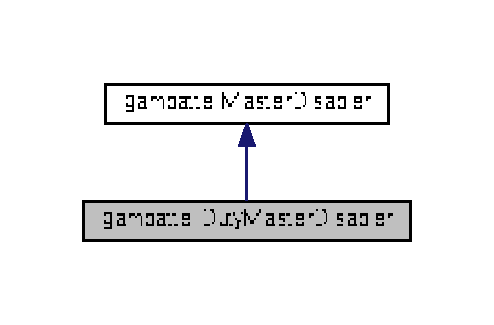
\includegraphics[width=237pt]{classgambatte_1_1DutyMasterDisabler__inherit__graph}
\end{center}
\end{figure}


Collaboration diagram for gambatte\+:\+:Duty\+Master\+Disabler\+:
\nopagebreak
\begin{figure}[H]
\begin{center}
\leavevmode
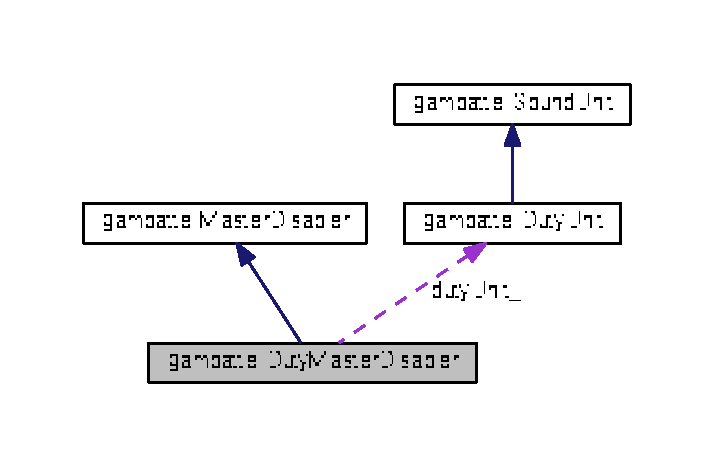
\includegraphics[width=343pt]{classgambatte_1_1DutyMasterDisabler__coll__graph}
\end{center}
\end{figure}
\subsection*{Public Member Functions}
\begin{DoxyCompactItemize}
\item 
\hyperlink{classgambatte_1_1DutyMasterDisabler_ab529f2ecc1ead79810197e3d786894e2}{Duty\+Master\+Disabler} (bool \&m, \hyperlink{classgambatte_1_1DutyUnit}{Duty\+Unit} \&duty\+Unit)
\item 
virtual void \hyperlink{classgambatte_1_1DutyMasterDisabler_a21f513f0b20eae19255a473668a099f6}{operator()} ()
\end{DoxyCompactItemize}
\subsection*{Private Attributes}
\begin{DoxyCompactItemize}
\item 
\hyperlink{classgambatte_1_1DutyUnit}{Duty\+Unit} \& \hyperlink{classgambatte_1_1DutyMasterDisabler_a972464d15d13fd132dd1a9266f39bc13}{duty\+Unit\+\_\+}
\end{DoxyCompactItemize}


\subsection{Constructor \& Destructor Documentation}
\mbox{\Hypertarget{classgambatte_1_1DutyMasterDisabler_ab529f2ecc1ead79810197e3d786894e2}\label{classgambatte_1_1DutyMasterDisabler_ab529f2ecc1ead79810197e3d786894e2}} 
\index{gambatte\+::\+Duty\+Master\+Disabler@{gambatte\+::\+Duty\+Master\+Disabler}!Duty\+Master\+Disabler@{Duty\+Master\+Disabler}}
\index{Duty\+Master\+Disabler@{Duty\+Master\+Disabler}!gambatte\+::\+Duty\+Master\+Disabler@{gambatte\+::\+Duty\+Master\+Disabler}}
\subsubsection{\texorpdfstring{Duty\+Master\+Disabler()}{DutyMasterDisabler()}}
{\footnotesize\ttfamily gambatte\+::\+Duty\+Master\+Disabler\+::\+Duty\+Master\+Disabler (\begin{DoxyParamCaption}\item[{bool \&}]{m,  }\item[{\hyperlink{classgambatte_1_1DutyUnit}{Duty\+Unit} \&}]{duty\+Unit }\end{DoxyParamCaption})\hspace{0.3cm}{\ttfamily [inline]}}



\subsection{Member Function Documentation}
\mbox{\Hypertarget{classgambatte_1_1DutyMasterDisabler_a21f513f0b20eae19255a473668a099f6}\label{classgambatte_1_1DutyMasterDisabler_a21f513f0b20eae19255a473668a099f6}} 
\index{gambatte\+::\+Duty\+Master\+Disabler@{gambatte\+::\+Duty\+Master\+Disabler}!operator()@{operator()}}
\index{operator()@{operator()}!gambatte\+::\+Duty\+Master\+Disabler@{gambatte\+::\+Duty\+Master\+Disabler}}
\subsubsection{\texorpdfstring{operator()()}{operator()()}}
{\footnotesize\ttfamily virtual void gambatte\+::\+Duty\+Master\+Disabler\+::operator() (\begin{DoxyParamCaption}{ }\end{DoxyParamCaption})\hspace{0.3cm}{\ttfamily [inline]}, {\ttfamily [virtual]}}



Reimplemented from \hyperlink{classgambatte_1_1MasterDisabler_a6b69f64af3e8112eac3767a74ee0e322}{gambatte\+::\+Master\+Disabler}.



\subsection{Member Data Documentation}
\mbox{\Hypertarget{classgambatte_1_1DutyMasterDisabler_a972464d15d13fd132dd1a9266f39bc13}\label{classgambatte_1_1DutyMasterDisabler_a972464d15d13fd132dd1a9266f39bc13}} 
\index{gambatte\+::\+Duty\+Master\+Disabler@{gambatte\+::\+Duty\+Master\+Disabler}!duty\+Unit\+\_\+@{duty\+Unit\+\_\+}}
\index{duty\+Unit\+\_\+@{duty\+Unit\+\_\+}!gambatte\+::\+Duty\+Master\+Disabler@{gambatte\+::\+Duty\+Master\+Disabler}}
\subsubsection{\texorpdfstring{duty\+Unit\+\_\+}{dutyUnit\_}}
{\footnotesize\ttfamily \hyperlink{classgambatte_1_1DutyUnit}{Duty\+Unit}\& gambatte\+::\+Duty\+Master\+Disabler\+::duty\+Unit\+\_\+\hspace{0.3cm}{\ttfamily [private]}}



The documentation for this class was generated from the following file\+:\begin{DoxyCompactItemize}
\item 
src/sound/\hyperlink{duty__unit_8h}{duty\+\_\+unit.\+h}\end{DoxyCompactItemize}

\hypertarget{classgambatte_1_1DutyUnit}{}\section{gambatte\+:\+:Duty\+Unit Class Reference}
\label{classgambatte_1_1DutyUnit}\index{gambatte\+::\+Duty\+Unit@{gambatte\+::\+Duty\+Unit}}


{\ttfamily \#include $<$duty\+\_\+unit.\+h$>$}



Inheritance diagram for gambatte\+:\+:Duty\+Unit\+:\nopagebreak
\begin{figure}[H]
\begin{center}
\leavevmode
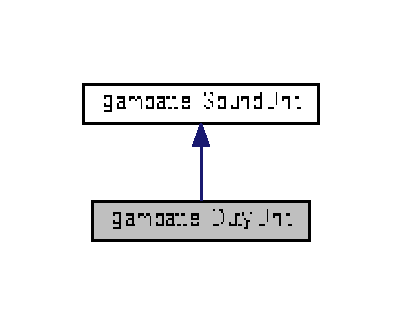
\includegraphics[width=193pt]{classgambatte_1_1DutyUnit__inherit__graph}
\end{center}
\end{figure}


Collaboration diagram for gambatte\+:\+:Duty\+Unit\+:\nopagebreak
\begin{figure}[H]
\begin{center}
\leavevmode
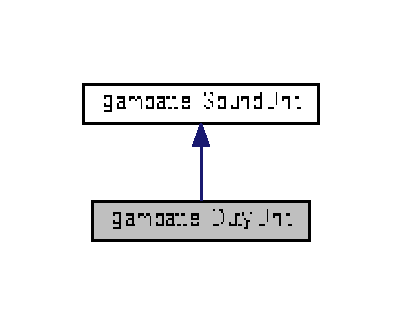
\includegraphics[width=193pt]{classgambatte_1_1DutyUnit__coll__graph}
\end{center}
\end{figure}
\subsection*{Public Member Functions}
\begin{DoxyCompactItemize}
\item 
\hyperlink{classgambatte_1_1DutyUnit_a4313410af8c15cb68eb276df92639b86}{Duty\+Unit} ()
\item 
virtual void \hyperlink{classgambatte_1_1DutyUnit_a2f051bb4772d30c58f2e88b85e947e61}{event} ()
\item 
virtual void \hyperlink{classgambatte_1_1DutyUnit_a69b982611026639129fda42e637e7b12}{reset\+Counters} (unsigned old\+Cc)
\item 
bool \hyperlink{classgambatte_1_1DutyUnit_a8c1e7cb1c7de208555b585e565b134c9}{is\+High\+State} () const
\item 
void \hyperlink{classgambatte_1_1DutyUnit_a5ba57779a4204bfc729b69f4d4304597}{nr1\+Change} (unsigned new\+Nr1, unsigned cc)
\item 
void \hyperlink{classgambatte_1_1DutyUnit_a6ef2e5973a348588ab05f78f93de6295}{nr3\+Change} (unsigned new\+Nr3, unsigned cc)
\item 
void \hyperlink{classgambatte_1_1DutyUnit_aa7e53abb8b26dca277a0447da8dad150}{nr4\+Change} (unsigned new\+Nr4, unsigned cc)
\item 
void \hyperlink{classgambatte_1_1DutyUnit_a0062af72b8d6b7220e82109b53f5e250}{reset} ()
\item 
void \hyperlink{classgambatte_1_1DutyUnit_a2326dd372384fb52466e307946717f65}{save\+State} (\hyperlink{structgambatte_1_1SaveState_1_1SPU_1_1Duty}{Save\+State\+::\+S\+P\+U\+::\+Duty} \&dstate, unsigned cc)
\item 
void \hyperlink{classgambatte_1_1DutyUnit_a64f049070cbd7ba7157410953186312b}{load\+State} (\hyperlink{structgambatte_1_1SaveState_1_1SPU_1_1Duty}{Save\+State\+::\+S\+P\+U\+::\+Duty} const \&dstate, unsigned nr1, unsigned nr4, unsigned cc)
\item 
void \hyperlink{classgambatte_1_1DutyUnit_a9def301fa5ff4359c4793a5fda3eb09c}{kill\+Counter} ()
\item 
void \hyperlink{classgambatte_1_1DutyUnit_a80e058f8c2210c9e7a52cceecaac4cde}{revive\+Counter} (unsigned cc)
\item 
void \hyperlink{classgambatte_1_1DutyUnit_adfb8ad7e89551ee6c384e010fa51fba6}{load\+Or\+Save} (\hyperlink{classgambatte_1_1loadsave}{loadsave} \&\hyperlink{ppu_8cpp_a2f2eca6997ee7baf8901725ae074d45b}{state})
\item 
unsigned \hyperlink{classgambatte_1_1DutyUnit_a2533194e4d5e582e962fe19b84377b70}{freq} () const
\item 
void \hyperlink{classgambatte_1_1DutyUnit_ac852c8510e1b1c8c0d7e8a63270167bf}{set\+Freq} (unsigned new\+Freq, unsigned cc)
\end{DoxyCompactItemize}
\subsection*{Private Member Functions}
\begin{DoxyCompactItemize}
\item 
void \hyperlink{classgambatte_1_1DutyUnit_ac47abbcf178693d44cf747459afaebf2}{set\+Counter} ()
\item 
void \hyperlink{classgambatte_1_1DutyUnit_a1cc5dd0b49b65816128ee3d52303c27d}{set\+Duty} (unsigned nr1)
\item 
void \hyperlink{classgambatte_1_1DutyUnit_ad972c3aa4b864ef85abc3c84ef1a24dd}{update\+Pos} (unsigned cc)
\end{DoxyCompactItemize}
\subsection*{Private Attributes}
\begin{DoxyCompactItemize}
\item 
unsigned \hyperlink{classgambatte_1_1DutyUnit_a79613bf1e29067922acc8404aa965cc5}{next\+Pos\+Update\+\_\+}
\item 
unsigned short \hyperlink{classgambatte_1_1DutyUnit_ab7744a1a9d16bb7226a401e5e02452fe}{period\+\_\+}
\item 
unsigned char \hyperlink{classgambatte_1_1DutyUnit_a357ce9a2491fe91fa402d21b1ca7805e}{pos\+\_\+}
\item 
unsigned char \hyperlink{classgambatte_1_1DutyUnit_a35b7a7b47842abd813f91ab73cbe1dd2}{duty\+\_\+}
\item 
bool \hyperlink{classgambatte_1_1DutyUnit_afe7cae5f88b8e9f5402cb7b4970c4a47}{high\+\_\+}
\item 
bool \hyperlink{classgambatte_1_1DutyUnit_a9f7634538a43cd88af58f406b92f55d7}{enable\+Events\+\_\+}
\end{DoxyCompactItemize}
\subsection*{Additional Inherited Members}


\subsection{Constructor \& Destructor Documentation}
\mbox{\Hypertarget{classgambatte_1_1DutyUnit_a4313410af8c15cb68eb276df92639b86}\label{classgambatte_1_1DutyUnit_a4313410af8c15cb68eb276df92639b86}} 
\index{gambatte\+::\+Duty\+Unit@{gambatte\+::\+Duty\+Unit}!Duty\+Unit@{Duty\+Unit}}
\index{Duty\+Unit@{Duty\+Unit}!gambatte\+::\+Duty\+Unit@{gambatte\+::\+Duty\+Unit}}
\subsubsection{\texorpdfstring{Duty\+Unit()}{DutyUnit()}}
{\footnotesize\ttfamily gambatte\+::\+Duty\+Unit\+::\+Duty\+Unit (\begin{DoxyParamCaption}{ }\end{DoxyParamCaption})}



\subsection{Member Function Documentation}
\mbox{\Hypertarget{classgambatte_1_1DutyUnit_a2f051bb4772d30c58f2e88b85e947e61}\label{classgambatte_1_1DutyUnit_a2f051bb4772d30c58f2e88b85e947e61}} 
\index{gambatte\+::\+Duty\+Unit@{gambatte\+::\+Duty\+Unit}!event@{event}}
\index{event@{event}!gambatte\+::\+Duty\+Unit@{gambatte\+::\+Duty\+Unit}}
\subsubsection{\texorpdfstring{event()}{event()}}
{\footnotesize\ttfamily void gambatte\+::\+Duty\+Unit\+::event (\begin{DoxyParamCaption}{ }\end{DoxyParamCaption})\hspace{0.3cm}{\ttfamily [virtual]}}



Implements \hyperlink{classgambatte_1_1SoundUnit_a8ad6df87fc3700d9d3bee470383197b4}{gambatte\+::\+Sound\+Unit}.

\mbox{\Hypertarget{classgambatte_1_1DutyUnit_a2533194e4d5e582e962fe19b84377b70}\label{classgambatte_1_1DutyUnit_a2533194e4d5e582e962fe19b84377b70}} 
\index{gambatte\+::\+Duty\+Unit@{gambatte\+::\+Duty\+Unit}!freq@{freq}}
\index{freq@{freq}!gambatte\+::\+Duty\+Unit@{gambatte\+::\+Duty\+Unit}}
\subsubsection{\texorpdfstring{freq()}{freq()}}
{\footnotesize\ttfamily unsigned gambatte\+::\+Duty\+Unit\+::freq (\begin{DoxyParamCaption}{ }\end{DoxyParamCaption}) const\hspace{0.3cm}{\ttfamily [inline]}}

\mbox{\Hypertarget{classgambatte_1_1DutyUnit_a8c1e7cb1c7de208555b585e565b134c9}\label{classgambatte_1_1DutyUnit_a8c1e7cb1c7de208555b585e565b134c9}} 
\index{gambatte\+::\+Duty\+Unit@{gambatte\+::\+Duty\+Unit}!is\+High\+State@{is\+High\+State}}
\index{is\+High\+State@{is\+High\+State}!gambatte\+::\+Duty\+Unit@{gambatte\+::\+Duty\+Unit}}
\subsubsection{\texorpdfstring{is\+High\+State()}{isHighState()}}
{\footnotesize\ttfamily bool gambatte\+::\+Duty\+Unit\+::is\+High\+State (\begin{DoxyParamCaption}{ }\end{DoxyParamCaption}) const\hspace{0.3cm}{\ttfamily [inline]}}

\mbox{\Hypertarget{classgambatte_1_1DutyUnit_a9def301fa5ff4359c4793a5fda3eb09c}\label{classgambatte_1_1DutyUnit_a9def301fa5ff4359c4793a5fda3eb09c}} 
\index{gambatte\+::\+Duty\+Unit@{gambatte\+::\+Duty\+Unit}!kill\+Counter@{kill\+Counter}}
\index{kill\+Counter@{kill\+Counter}!gambatte\+::\+Duty\+Unit@{gambatte\+::\+Duty\+Unit}}
\subsubsection{\texorpdfstring{kill\+Counter()}{killCounter()}}
{\footnotesize\ttfamily void gambatte\+::\+Duty\+Unit\+::kill\+Counter (\begin{DoxyParamCaption}{ }\end{DoxyParamCaption})}

\mbox{\Hypertarget{classgambatte_1_1DutyUnit_adfb8ad7e89551ee6c384e010fa51fba6}\label{classgambatte_1_1DutyUnit_adfb8ad7e89551ee6c384e010fa51fba6}} 
\index{gambatte\+::\+Duty\+Unit@{gambatte\+::\+Duty\+Unit}!load\+Or\+Save@{load\+Or\+Save}}
\index{load\+Or\+Save@{load\+Or\+Save}!gambatte\+::\+Duty\+Unit@{gambatte\+::\+Duty\+Unit}}
\subsubsection{\texorpdfstring{load\+Or\+Save()}{loadOrSave()}}
{\footnotesize\ttfamily void gambatte\+::\+Duty\+Unit\+::load\+Or\+Save (\begin{DoxyParamCaption}\item[{\hyperlink{classgambatte_1_1loadsave}{loadsave} \&}]{state }\end{DoxyParamCaption})}

\mbox{\Hypertarget{classgambatte_1_1DutyUnit_a64f049070cbd7ba7157410953186312b}\label{classgambatte_1_1DutyUnit_a64f049070cbd7ba7157410953186312b}} 
\index{gambatte\+::\+Duty\+Unit@{gambatte\+::\+Duty\+Unit}!load\+State@{load\+State}}
\index{load\+State@{load\+State}!gambatte\+::\+Duty\+Unit@{gambatte\+::\+Duty\+Unit}}
\subsubsection{\texorpdfstring{load\+State()}{loadState()}}
{\footnotesize\ttfamily void gambatte\+::\+Duty\+Unit\+::load\+State (\begin{DoxyParamCaption}\item[{\hyperlink{structgambatte_1_1SaveState_1_1SPU_1_1Duty}{Save\+State\+::\+S\+P\+U\+::\+Duty} const \&}]{dstate,  }\item[{unsigned}]{nr1,  }\item[{unsigned}]{nr4,  }\item[{unsigned}]{cc }\end{DoxyParamCaption})}

\mbox{\Hypertarget{classgambatte_1_1DutyUnit_a5ba57779a4204bfc729b69f4d4304597}\label{classgambatte_1_1DutyUnit_a5ba57779a4204bfc729b69f4d4304597}} 
\index{gambatte\+::\+Duty\+Unit@{gambatte\+::\+Duty\+Unit}!nr1\+Change@{nr1\+Change}}
\index{nr1\+Change@{nr1\+Change}!gambatte\+::\+Duty\+Unit@{gambatte\+::\+Duty\+Unit}}
\subsubsection{\texorpdfstring{nr1\+Change()}{nr1Change()}}
{\footnotesize\ttfamily void gambatte\+::\+Duty\+Unit\+::nr1\+Change (\begin{DoxyParamCaption}\item[{unsigned}]{new\+Nr1,  }\item[{unsigned}]{cc }\end{DoxyParamCaption})}

\mbox{\Hypertarget{classgambatte_1_1DutyUnit_a6ef2e5973a348588ab05f78f93de6295}\label{classgambatte_1_1DutyUnit_a6ef2e5973a348588ab05f78f93de6295}} 
\index{gambatte\+::\+Duty\+Unit@{gambatte\+::\+Duty\+Unit}!nr3\+Change@{nr3\+Change}}
\index{nr3\+Change@{nr3\+Change}!gambatte\+::\+Duty\+Unit@{gambatte\+::\+Duty\+Unit}}
\subsubsection{\texorpdfstring{nr3\+Change()}{nr3Change()}}
{\footnotesize\ttfamily void gambatte\+::\+Duty\+Unit\+::nr3\+Change (\begin{DoxyParamCaption}\item[{unsigned}]{new\+Nr3,  }\item[{unsigned}]{cc }\end{DoxyParamCaption})}

\mbox{\Hypertarget{classgambatte_1_1DutyUnit_aa7e53abb8b26dca277a0447da8dad150}\label{classgambatte_1_1DutyUnit_aa7e53abb8b26dca277a0447da8dad150}} 
\index{gambatte\+::\+Duty\+Unit@{gambatte\+::\+Duty\+Unit}!nr4\+Change@{nr4\+Change}}
\index{nr4\+Change@{nr4\+Change}!gambatte\+::\+Duty\+Unit@{gambatte\+::\+Duty\+Unit}}
\subsubsection{\texorpdfstring{nr4\+Change()}{nr4Change()}}
{\footnotesize\ttfamily void gambatte\+::\+Duty\+Unit\+::nr4\+Change (\begin{DoxyParamCaption}\item[{unsigned}]{new\+Nr4,  }\item[{unsigned}]{cc }\end{DoxyParamCaption})}

\mbox{\Hypertarget{classgambatte_1_1DutyUnit_a0062af72b8d6b7220e82109b53f5e250}\label{classgambatte_1_1DutyUnit_a0062af72b8d6b7220e82109b53f5e250}} 
\index{gambatte\+::\+Duty\+Unit@{gambatte\+::\+Duty\+Unit}!reset@{reset}}
\index{reset@{reset}!gambatte\+::\+Duty\+Unit@{gambatte\+::\+Duty\+Unit}}
\subsubsection{\texorpdfstring{reset()}{reset()}}
{\footnotesize\ttfamily void gambatte\+::\+Duty\+Unit\+::reset (\begin{DoxyParamCaption}{ }\end{DoxyParamCaption})}

\mbox{\Hypertarget{classgambatte_1_1DutyUnit_a69b982611026639129fda42e637e7b12}\label{classgambatte_1_1DutyUnit_a69b982611026639129fda42e637e7b12}} 
\index{gambatte\+::\+Duty\+Unit@{gambatte\+::\+Duty\+Unit}!reset\+Counters@{reset\+Counters}}
\index{reset\+Counters@{reset\+Counters}!gambatte\+::\+Duty\+Unit@{gambatte\+::\+Duty\+Unit}}
\subsubsection{\texorpdfstring{reset\+Counters()}{resetCounters()}}
{\footnotesize\ttfamily void gambatte\+::\+Duty\+Unit\+::reset\+Counters (\begin{DoxyParamCaption}\item[{unsigned}]{old\+Cc }\end{DoxyParamCaption})\hspace{0.3cm}{\ttfamily [virtual]}}



Reimplemented from \hyperlink{classgambatte_1_1SoundUnit_a3baa270f75463b24cd79fe5970103d4f}{gambatte\+::\+Sound\+Unit}.

\mbox{\Hypertarget{classgambatte_1_1DutyUnit_a80e058f8c2210c9e7a52cceecaac4cde}\label{classgambatte_1_1DutyUnit_a80e058f8c2210c9e7a52cceecaac4cde}} 
\index{gambatte\+::\+Duty\+Unit@{gambatte\+::\+Duty\+Unit}!revive\+Counter@{revive\+Counter}}
\index{revive\+Counter@{revive\+Counter}!gambatte\+::\+Duty\+Unit@{gambatte\+::\+Duty\+Unit}}
\subsubsection{\texorpdfstring{revive\+Counter()}{reviveCounter()}}
{\footnotesize\ttfamily void gambatte\+::\+Duty\+Unit\+::revive\+Counter (\begin{DoxyParamCaption}\item[{unsigned}]{cc }\end{DoxyParamCaption})}

\mbox{\Hypertarget{classgambatte_1_1DutyUnit_a2326dd372384fb52466e307946717f65}\label{classgambatte_1_1DutyUnit_a2326dd372384fb52466e307946717f65}} 
\index{gambatte\+::\+Duty\+Unit@{gambatte\+::\+Duty\+Unit}!save\+State@{save\+State}}
\index{save\+State@{save\+State}!gambatte\+::\+Duty\+Unit@{gambatte\+::\+Duty\+Unit}}
\subsubsection{\texorpdfstring{save\+State()}{saveState()}}
{\footnotesize\ttfamily void gambatte\+::\+Duty\+Unit\+::save\+State (\begin{DoxyParamCaption}\item[{\hyperlink{structgambatte_1_1SaveState_1_1SPU_1_1Duty}{Save\+State\+::\+S\+P\+U\+::\+Duty} \&}]{dstate,  }\item[{unsigned}]{cc }\end{DoxyParamCaption})}

\mbox{\Hypertarget{classgambatte_1_1DutyUnit_ac47abbcf178693d44cf747459afaebf2}\label{classgambatte_1_1DutyUnit_ac47abbcf178693d44cf747459afaebf2}} 
\index{gambatte\+::\+Duty\+Unit@{gambatte\+::\+Duty\+Unit}!set\+Counter@{set\+Counter}}
\index{set\+Counter@{set\+Counter}!gambatte\+::\+Duty\+Unit@{gambatte\+::\+Duty\+Unit}}
\subsubsection{\texorpdfstring{set\+Counter()}{setCounter()}}
{\footnotesize\ttfamily void gambatte\+::\+Duty\+Unit\+::set\+Counter (\begin{DoxyParamCaption}{ }\end{DoxyParamCaption})\hspace{0.3cm}{\ttfamily [private]}}

\mbox{\Hypertarget{classgambatte_1_1DutyUnit_a1cc5dd0b49b65816128ee3d52303c27d}\label{classgambatte_1_1DutyUnit_a1cc5dd0b49b65816128ee3d52303c27d}} 
\index{gambatte\+::\+Duty\+Unit@{gambatte\+::\+Duty\+Unit}!set\+Duty@{set\+Duty}}
\index{set\+Duty@{set\+Duty}!gambatte\+::\+Duty\+Unit@{gambatte\+::\+Duty\+Unit}}
\subsubsection{\texorpdfstring{set\+Duty()}{setDuty()}}
{\footnotesize\ttfamily void gambatte\+::\+Duty\+Unit\+::set\+Duty (\begin{DoxyParamCaption}\item[{unsigned}]{nr1 }\end{DoxyParamCaption})\hspace{0.3cm}{\ttfamily [private]}}

\mbox{\Hypertarget{classgambatte_1_1DutyUnit_ac852c8510e1b1c8c0d7e8a63270167bf}\label{classgambatte_1_1DutyUnit_ac852c8510e1b1c8c0d7e8a63270167bf}} 
\index{gambatte\+::\+Duty\+Unit@{gambatte\+::\+Duty\+Unit}!set\+Freq@{set\+Freq}}
\index{set\+Freq@{set\+Freq}!gambatte\+::\+Duty\+Unit@{gambatte\+::\+Duty\+Unit}}
\subsubsection{\texorpdfstring{set\+Freq()}{setFreq()}}
{\footnotesize\ttfamily void gambatte\+::\+Duty\+Unit\+::set\+Freq (\begin{DoxyParamCaption}\item[{unsigned}]{new\+Freq,  }\item[{unsigned}]{cc }\end{DoxyParamCaption})}

\mbox{\Hypertarget{classgambatte_1_1DutyUnit_ad972c3aa4b864ef85abc3c84ef1a24dd}\label{classgambatte_1_1DutyUnit_ad972c3aa4b864ef85abc3c84ef1a24dd}} 
\index{gambatte\+::\+Duty\+Unit@{gambatte\+::\+Duty\+Unit}!update\+Pos@{update\+Pos}}
\index{update\+Pos@{update\+Pos}!gambatte\+::\+Duty\+Unit@{gambatte\+::\+Duty\+Unit}}
\subsubsection{\texorpdfstring{update\+Pos()}{updatePos()}}
{\footnotesize\ttfamily void gambatte\+::\+Duty\+Unit\+::update\+Pos (\begin{DoxyParamCaption}\item[{unsigned}]{cc }\end{DoxyParamCaption})\hspace{0.3cm}{\ttfamily [private]}}



\subsection{Member Data Documentation}
\mbox{\Hypertarget{classgambatte_1_1DutyUnit_a35b7a7b47842abd813f91ab73cbe1dd2}\label{classgambatte_1_1DutyUnit_a35b7a7b47842abd813f91ab73cbe1dd2}} 
\index{gambatte\+::\+Duty\+Unit@{gambatte\+::\+Duty\+Unit}!duty\+\_\+@{duty\+\_\+}}
\index{duty\+\_\+@{duty\+\_\+}!gambatte\+::\+Duty\+Unit@{gambatte\+::\+Duty\+Unit}}
\subsubsection{\texorpdfstring{duty\+\_\+}{duty\_}}
{\footnotesize\ttfamily unsigned char gambatte\+::\+Duty\+Unit\+::duty\+\_\+\hspace{0.3cm}{\ttfamily [private]}}

\mbox{\Hypertarget{classgambatte_1_1DutyUnit_a9f7634538a43cd88af58f406b92f55d7}\label{classgambatte_1_1DutyUnit_a9f7634538a43cd88af58f406b92f55d7}} 
\index{gambatte\+::\+Duty\+Unit@{gambatte\+::\+Duty\+Unit}!enable\+Events\+\_\+@{enable\+Events\+\_\+}}
\index{enable\+Events\+\_\+@{enable\+Events\+\_\+}!gambatte\+::\+Duty\+Unit@{gambatte\+::\+Duty\+Unit}}
\subsubsection{\texorpdfstring{enable\+Events\+\_\+}{enableEvents\_}}
{\footnotesize\ttfamily bool gambatte\+::\+Duty\+Unit\+::enable\+Events\+\_\+\hspace{0.3cm}{\ttfamily [private]}}

\mbox{\Hypertarget{classgambatte_1_1DutyUnit_afe7cae5f88b8e9f5402cb7b4970c4a47}\label{classgambatte_1_1DutyUnit_afe7cae5f88b8e9f5402cb7b4970c4a47}} 
\index{gambatte\+::\+Duty\+Unit@{gambatte\+::\+Duty\+Unit}!high\+\_\+@{high\+\_\+}}
\index{high\+\_\+@{high\+\_\+}!gambatte\+::\+Duty\+Unit@{gambatte\+::\+Duty\+Unit}}
\subsubsection{\texorpdfstring{high\+\_\+}{high\_}}
{\footnotesize\ttfamily bool gambatte\+::\+Duty\+Unit\+::high\+\_\+\hspace{0.3cm}{\ttfamily [private]}}

\mbox{\Hypertarget{classgambatte_1_1DutyUnit_a79613bf1e29067922acc8404aa965cc5}\label{classgambatte_1_1DutyUnit_a79613bf1e29067922acc8404aa965cc5}} 
\index{gambatte\+::\+Duty\+Unit@{gambatte\+::\+Duty\+Unit}!next\+Pos\+Update\+\_\+@{next\+Pos\+Update\+\_\+}}
\index{next\+Pos\+Update\+\_\+@{next\+Pos\+Update\+\_\+}!gambatte\+::\+Duty\+Unit@{gambatte\+::\+Duty\+Unit}}
\subsubsection{\texorpdfstring{next\+Pos\+Update\+\_\+}{nextPosUpdate\_}}
{\footnotesize\ttfamily unsigned gambatte\+::\+Duty\+Unit\+::next\+Pos\+Update\+\_\+\hspace{0.3cm}{\ttfamily [private]}}

\mbox{\Hypertarget{classgambatte_1_1DutyUnit_ab7744a1a9d16bb7226a401e5e02452fe}\label{classgambatte_1_1DutyUnit_ab7744a1a9d16bb7226a401e5e02452fe}} 
\index{gambatte\+::\+Duty\+Unit@{gambatte\+::\+Duty\+Unit}!period\+\_\+@{period\+\_\+}}
\index{period\+\_\+@{period\+\_\+}!gambatte\+::\+Duty\+Unit@{gambatte\+::\+Duty\+Unit}}
\subsubsection{\texorpdfstring{period\+\_\+}{period\_}}
{\footnotesize\ttfamily unsigned short gambatte\+::\+Duty\+Unit\+::period\+\_\+\hspace{0.3cm}{\ttfamily [private]}}

\mbox{\Hypertarget{classgambatte_1_1DutyUnit_a357ce9a2491fe91fa402d21b1ca7805e}\label{classgambatte_1_1DutyUnit_a357ce9a2491fe91fa402d21b1ca7805e}} 
\index{gambatte\+::\+Duty\+Unit@{gambatte\+::\+Duty\+Unit}!pos\+\_\+@{pos\+\_\+}}
\index{pos\+\_\+@{pos\+\_\+}!gambatte\+::\+Duty\+Unit@{gambatte\+::\+Duty\+Unit}}
\subsubsection{\texorpdfstring{pos\+\_\+}{pos\_}}
{\footnotesize\ttfamily unsigned char gambatte\+::\+Duty\+Unit\+::pos\+\_\+\hspace{0.3cm}{\ttfamily [private]}}



The documentation for this class was generated from the following files\+:\begin{DoxyCompactItemize}
\item 
src/sound/\hyperlink{duty__unit_8h}{duty\+\_\+unit.\+h}\item 
src/sound/\hyperlink{duty__unit_8cpp}{duty\+\_\+unit.\+cpp}\end{DoxyCompactItemize}

\hypertarget{structgambatte_1_1SaveState_1_1SPU_1_1Env}{}\section{gambatte\+:\+:Save\+State\+:\+:S\+PU\+:\+:Env Struct Reference}
\label{structgambatte_1_1SaveState_1_1SPU_1_1Env}\index{gambatte\+::\+Save\+State\+::\+S\+P\+U\+::\+Env@{gambatte\+::\+Save\+State\+::\+S\+P\+U\+::\+Env}}


{\ttfamily \#include $<$savestate.\+h$>$}

\subsection*{Public Attributes}
\begin{DoxyCompactItemize}
\item 
unsigned \hyperlink{structgambatte_1_1SaveState_1_1SPU_1_1Env_a7b82be49c81e3e4ceaba2298c706a03c}{counter}
\item 
unsigned char \hyperlink{structgambatte_1_1SaveState_1_1SPU_1_1Env_a3433ecacf201c5bd40b7c3606cc39445}{volume}
\end{DoxyCompactItemize}


\subsection{Member Data Documentation}
\mbox{\Hypertarget{structgambatte_1_1SaveState_1_1SPU_1_1Env_a7b82be49c81e3e4ceaba2298c706a03c}\label{structgambatte_1_1SaveState_1_1SPU_1_1Env_a7b82be49c81e3e4ceaba2298c706a03c}} 
\index{gambatte\+::\+Save\+State\+::\+S\+P\+U\+::\+Env@{gambatte\+::\+Save\+State\+::\+S\+P\+U\+::\+Env}!counter@{counter}}
\index{counter@{counter}!gambatte\+::\+Save\+State\+::\+S\+P\+U\+::\+Env@{gambatte\+::\+Save\+State\+::\+S\+P\+U\+::\+Env}}
\subsubsection{\texorpdfstring{counter}{counter}}
{\footnotesize\ttfamily unsigned gambatte\+::\+Save\+State\+::\+S\+P\+U\+::\+Env\+::counter}

\mbox{\Hypertarget{structgambatte_1_1SaveState_1_1SPU_1_1Env_a3433ecacf201c5bd40b7c3606cc39445}\label{structgambatte_1_1SaveState_1_1SPU_1_1Env_a3433ecacf201c5bd40b7c3606cc39445}} 
\index{gambatte\+::\+Save\+State\+::\+S\+P\+U\+::\+Env@{gambatte\+::\+Save\+State\+::\+S\+P\+U\+::\+Env}!volume@{volume}}
\index{volume@{volume}!gambatte\+::\+Save\+State\+::\+S\+P\+U\+::\+Env@{gambatte\+::\+Save\+State\+::\+S\+P\+U\+::\+Env}}
\subsubsection{\texorpdfstring{volume}{volume}}
{\footnotesize\ttfamily unsigned char gambatte\+::\+Save\+State\+::\+S\+P\+U\+::\+Env\+::volume}



The documentation for this struct was generated from the following file\+:\begin{DoxyCompactItemize}
\item 
src/\hyperlink{savestate_8h}{savestate.\+h}\end{DoxyCompactItemize}

\hypertarget{classgambatte_1_1EnvelopeUnit}{}\section{gambatte\+:\+:Envelope\+Unit Class Reference}
\label{classgambatte_1_1EnvelopeUnit}\index{gambatte\+::\+Envelope\+Unit@{gambatte\+::\+Envelope\+Unit}}


{\ttfamily \#include $<$envelope\+\_\+unit.\+h$>$}



Inheritance diagram for gambatte\+:\+:Envelope\+Unit\+:\nopagebreak
\begin{figure}[H]
\begin{center}
\leavevmode
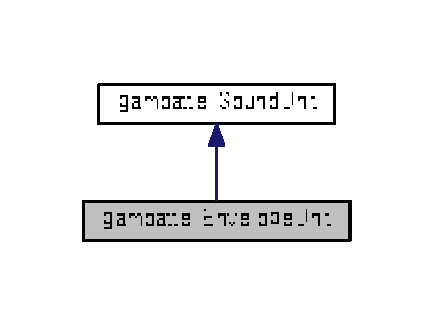
\includegraphics[width=208pt]{classgambatte_1_1EnvelopeUnit__inherit__graph}
\end{center}
\end{figure}


Collaboration diagram for gambatte\+:\+:Envelope\+Unit\+:
\nopagebreak
\begin{figure}[H]
\begin{center}
\leavevmode
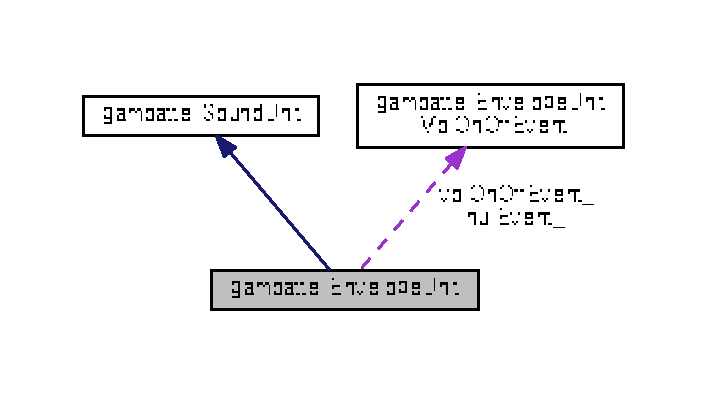
\includegraphics[width=340pt]{classgambatte_1_1EnvelopeUnit__coll__graph}
\end{center}
\end{figure}
\subsection*{Classes}
\begin{DoxyCompactItemize}
\item 
struct \hyperlink{structgambatte_1_1EnvelopeUnit_1_1VolOnOffEvent}{Vol\+On\+Off\+Event}
\end{DoxyCompactItemize}
\subsection*{Public Member Functions}
\begin{DoxyCompactItemize}
\item 
\hyperlink{classgambatte_1_1EnvelopeUnit_af86bedf9a96074c5ee17121e25ceb087}{Envelope\+Unit} (\hyperlink{structgambatte_1_1EnvelopeUnit_1_1VolOnOffEvent}{Vol\+On\+Off\+Event} \&vol\+On\+Off\+Event=\hyperlink{classgambatte_1_1EnvelopeUnit_a0d3bffc1ee1ab27933ad8e602f3306b8}{null\+Event\+\_\+})
\item 
void \hyperlink{classgambatte_1_1EnvelopeUnit_a9273d36ce1ef6e3e11a4d2bb0d3bc367}{event} ()
\item 
bool \hyperlink{classgambatte_1_1EnvelopeUnit_a506dc8beed37a81428113f501192e199}{dac\+Is\+On} () const
\item 
unsigned \hyperlink{classgambatte_1_1EnvelopeUnit_ae41f480cc569c22ab11923bca08a4acd}{get\+Volume} () const
\item 
bool \hyperlink{classgambatte_1_1EnvelopeUnit_ad7c7a2f2d1c323a39e15aac8f99a5101}{nr2\+Change} (unsigned new\+Nr2)
\item 
bool \hyperlink{classgambatte_1_1EnvelopeUnit_abf4a0224ded8cc63701e587018d52581}{nr4\+Init} (unsigned cycle\+Counter)
\item 
void \hyperlink{classgambatte_1_1EnvelopeUnit_a46bdeff4254f0cd99f8031c18c08de4b}{reset} ()
\item 
void \hyperlink{classgambatte_1_1EnvelopeUnit_ab1dba98c6654a5497d7ea6cd3bcc923a}{save\+State} (\hyperlink{structgambatte_1_1SaveState_1_1SPU_1_1Env}{Save\+State\+::\+S\+P\+U\+::\+Env} \&estate) const
\item 
void \hyperlink{classgambatte_1_1EnvelopeUnit_a1c9a90a54ae035d54c9c8e48848aca36}{load\+Or\+Save} (\hyperlink{classgambatte_1_1loadsave}{loadsave} \&\hyperlink{ppu_8cpp_a2f2eca6997ee7baf8901725ae074d45b}{state})
\item 
void \hyperlink{classgambatte_1_1EnvelopeUnit_a3377c470989ee2ef9b60d9e2af1fca50}{load\+State} (\hyperlink{structgambatte_1_1SaveState_1_1SPU_1_1Env}{Save\+State\+::\+S\+P\+U\+::\+Env} const \&estate, unsigned nr2, unsigned cc)
\end{DoxyCompactItemize}
\subsection*{Private Attributes}
\begin{DoxyCompactItemize}
\item 
\hyperlink{structgambatte_1_1EnvelopeUnit_1_1VolOnOffEvent}{Vol\+On\+Off\+Event} \& \hyperlink{classgambatte_1_1EnvelopeUnit_af3da8f1a21e7d450e1e8433b0add7df2}{vol\+On\+Off\+Event\+\_\+}
\item 
unsigned char \hyperlink{classgambatte_1_1EnvelopeUnit_a952e5d76b125e13c2d70988205eabaec}{nr2\+\_\+}
\item 
unsigned char \hyperlink{classgambatte_1_1EnvelopeUnit_a379080f901081f2b571161961fbef627}{volume\+\_\+}
\end{DoxyCompactItemize}
\subsection*{Static Private Attributes}
\begin{DoxyCompactItemize}
\item 
static \hyperlink{structgambatte_1_1EnvelopeUnit_1_1VolOnOffEvent}{Vol\+On\+Off\+Event} \hyperlink{classgambatte_1_1EnvelopeUnit_a0d3bffc1ee1ab27933ad8e602f3306b8}{null\+Event\+\_\+}
\end{DoxyCompactItemize}
\subsection*{Additional Inherited Members}


\subsection{Constructor \& Destructor Documentation}
\mbox{\Hypertarget{classgambatte_1_1EnvelopeUnit_af86bedf9a96074c5ee17121e25ceb087}\label{classgambatte_1_1EnvelopeUnit_af86bedf9a96074c5ee17121e25ceb087}} 
\index{gambatte\+::\+Envelope\+Unit@{gambatte\+::\+Envelope\+Unit}!Envelope\+Unit@{Envelope\+Unit}}
\index{Envelope\+Unit@{Envelope\+Unit}!gambatte\+::\+Envelope\+Unit@{gambatte\+::\+Envelope\+Unit}}
\subsubsection{\texorpdfstring{Envelope\+Unit()}{EnvelopeUnit()}}
{\footnotesize\ttfamily gambatte\+::\+Envelope\+Unit\+::\+Envelope\+Unit (\begin{DoxyParamCaption}\item[{\hyperlink{structgambatte_1_1EnvelopeUnit_1_1VolOnOffEvent}{Vol\+On\+Off\+Event} \&}]{vol\+On\+Off\+Event = {\ttfamily \hyperlink{classgambatte_1_1EnvelopeUnit_a0d3bffc1ee1ab27933ad8e602f3306b8}{null\+Event\+\_\+}} }\end{DoxyParamCaption})\hspace{0.3cm}{\ttfamily [explicit]}}



\subsection{Member Function Documentation}
\mbox{\Hypertarget{classgambatte_1_1EnvelopeUnit_a506dc8beed37a81428113f501192e199}\label{classgambatte_1_1EnvelopeUnit_a506dc8beed37a81428113f501192e199}} 
\index{gambatte\+::\+Envelope\+Unit@{gambatte\+::\+Envelope\+Unit}!dac\+Is\+On@{dac\+Is\+On}}
\index{dac\+Is\+On@{dac\+Is\+On}!gambatte\+::\+Envelope\+Unit@{gambatte\+::\+Envelope\+Unit}}
\subsubsection{\texorpdfstring{dac\+Is\+On()}{dacIsOn()}}
{\footnotesize\ttfamily bool gambatte\+::\+Envelope\+Unit\+::dac\+Is\+On (\begin{DoxyParamCaption}{ }\end{DoxyParamCaption}) const\hspace{0.3cm}{\ttfamily [inline]}}

\mbox{\Hypertarget{classgambatte_1_1EnvelopeUnit_a9273d36ce1ef6e3e11a4d2bb0d3bc367}\label{classgambatte_1_1EnvelopeUnit_a9273d36ce1ef6e3e11a4d2bb0d3bc367}} 
\index{gambatte\+::\+Envelope\+Unit@{gambatte\+::\+Envelope\+Unit}!event@{event}}
\index{event@{event}!gambatte\+::\+Envelope\+Unit@{gambatte\+::\+Envelope\+Unit}}
\subsubsection{\texorpdfstring{event()}{event()}}
{\footnotesize\ttfamily void gambatte\+::\+Envelope\+Unit\+::event (\begin{DoxyParamCaption}{ }\end{DoxyParamCaption})\hspace{0.3cm}{\ttfamily [virtual]}}



Implements \hyperlink{classgambatte_1_1SoundUnit_a8ad6df87fc3700d9d3bee470383197b4}{gambatte\+::\+Sound\+Unit}.

\mbox{\Hypertarget{classgambatte_1_1EnvelopeUnit_ae41f480cc569c22ab11923bca08a4acd}\label{classgambatte_1_1EnvelopeUnit_ae41f480cc569c22ab11923bca08a4acd}} 
\index{gambatte\+::\+Envelope\+Unit@{gambatte\+::\+Envelope\+Unit}!get\+Volume@{get\+Volume}}
\index{get\+Volume@{get\+Volume}!gambatte\+::\+Envelope\+Unit@{gambatte\+::\+Envelope\+Unit}}
\subsubsection{\texorpdfstring{get\+Volume()}{getVolume()}}
{\footnotesize\ttfamily unsigned gambatte\+::\+Envelope\+Unit\+::get\+Volume (\begin{DoxyParamCaption}{ }\end{DoxyParamCaption}) const\hspace{0.3cm}{\ttfamily [inline]}}

\mbox{\Hypertarget{classgambatte_1_1EnvelopeUnit_a1c9a90a54ae035d54c9c8e48848aca36}\label{classgambatte_1_1EnvelopeUnit_a1c9a90a54ae035d54c9c8e48848aca36}} 
\index{gambatte\+::\+Envelope\+Unit@{gambatte\+::\+Envelope\+Unit}!load\+Or\+Save@{load\+Or\+Save}}
\index{load\+Or\+Save@{load\+Or\+Save}!gambatte\+::\+Envelope\+Unit@{gambatte\+::\+Envelope\+Unit}}
\subsubsection{\texorpdfstring{load\+Or\+Save()}{loadOrSave()}}
{\footnotesize\ttfamily void gambatte\+::\+Envelope\+Unit\+::load\+Or\+Save (\begin{DoxyParamCaption}\item[{\hyperlink{classgambatte_1_1loadsave}{loadsave} \&}]{state }\end{DoxyParamCaption})}

\mbox{\Hypertarget{classgambatte_1_1EnvelopeUnit_a3377c470989ee2ef9b60d9e2af1fca50}\label{classgambatte_1_1EnvelopeUnit_a3377c470989ee2ef9b60d9e2af1fca50}} 
\index{gambatte\+::\+Envelope\+Unit@{gambatte\+::\+Envelope\+Unit}!load\+State@{load\+State}}
\index{load\+State@{load\+State}!gambatte\+::\+Envelope\+Unit@{gambatte\+::\+Envelope\+Unit}}
\subsubsection{\texorpdfstring{load\+State()}{loadState()}}
{\footnotesize\ttfamily void gambatte\+::\+Envelope\+Unit\+::load\+State (\begin{DoxyParamCaption}\item[{\hyperlink{structgambatte_1_1SaveState_1_1SPU_1_1Env}{Save\+State\+::\+S\+P\+U\+::\+Env} const \&}]{estate,  }\item[{unsigned}]{nr2,  }\item[{unsigned}]{cc }\end{DoxyParamCaption})}

\mbox{\Hypertarget{classgambatte_1_1EnvelopeUnit_ad7c7a2f2d1c323a39e15aac8f99a5101}\label{classgambatte_1_1EnvelopeUnit_ad7c7a2f2d1c323a39e15aac8f99a5101}} 
\index{gambatte\+::\+Envelope\+Unit@{gambatte\+::\+Envelope\+Unit}!nr2\+Change@{nr2\+Change}}
\index{nr2\+Change@{nr2\+Change}!gambatte\+::\+Envelope\+Unit@{gambatte\+::\+Envelope\+Unit}}
\subsubsection{\texorpdfstring{nr2\+Change()}{nr2Change()}}
{\footnotesize\ttfamily bool gambatte\+::\+Envelope\+Unit\+::nr2\+Change (\begin{DoxyParamCaption}\item[{unsigned}]{new\+Nr2 }\end{DoxyParamCaption})}

\mbox{\Hypertarget{classgambatte_1_1EnvelopeUnit_abf4a0224ded8cc63701e587018d52581}\label{classgambatte_1_1EnvelopeUnit_abf4a0224ded8cc63701e587018d52581}} 
\index{gambatte\+::\+Envelope\+Unit@{gambatte\+::\+Envelope\+Unit}!nr4\+Init@{nr4\+Init}}
\index{nr4\+Init@{nr4\+Init}!gambatte\+::\+Envelope\+Unit@{gambatte\+::\+Envelope\+Unit}}
\subsubsection{\texorpdfstring{nr4\+Init()}{nr4Init()}}
{\footnotesize\ttfamily bool gambatte\+::\+Envelope\+Unit\+::nr4\+Init (\begin{DoxyParamCaption}\item[{unsigned}]{cycle\+Counter }\end{DoxyParamCaption})}

\mbox{\Hypertarget{classgambatte_1_1EnvelopeUnit_a46bdeff4254f0cd99f8031c18c08de4b}\label{classgambatte_1_1EnvelopeUnit_a46bdeff4254f0cd99f8031c18c08de4b}} 
\index{gambatte\+::\+Envelope\+Unit@{gambatte\+::\+Envelope\+Unit}!reset@{reset}}
\index{reset@{reset}!gambatte\+::\+Envelope\+Unit@{gambatte\+::\+Envelope\+Unit}}
\subsubsection{\texorpdfstring{reset()}{reset()}}
{\footnotesize\ttfamily void gambatte\+::\+Envelope\+Unit\+::reset (\begin{DoxyParamCaption}{ }\end{DoxyParamCaption})}

\mbox{\Hypertarget{classgambatte_1_1EnvelopeUnit_ab1dba98c6654a5497d7ea6cd3bcc923a}\label{classgambatte_1_1EnvelopeUnit_ab1dba98c6654a5497d7ea6cd3bcc923a}} 
\index{gambatte\+::\+Envelope\+Unit@{gambatte\+::\+Envelope\+Unit}!save\+State@{save\+State}}
\index{save\+State@{save\+State}!gambatte\+::\+Envelope\+Unit@{gambatte\+::\+Envelope\+Unit}}
\subsubsection{\texorpdfstring{save\+State()}{saveState()}}
{\footnotesize\ttfamily void gambatte\+::\+Envelope\+Unit\+::save\+State (\begin{DoxyParamCaption}\item[{\hyperlink{structgambatte_1_1SaveState_1_1SPU_1_1Env}{Save\+State\+::\+S\+P\+U\+::\+Env} \&}]{estate }\end{DoxyParamCaption}) const}



\subsection{Member Data Documentation}
\mbox{\Hypertarget{classgambatte_1_1EnvelopeUnit_a952e5d76b125e13c2d70988205eabaec}\label{classgambatte_1_1EnvelopeUnit_a952e5d76b125e13c2d70988205eabaec}} 
\index{gambatte\+::\+Envelope\+Unit@{gambatte\+::\+Envelope\+Unit}!nr2\+\_\+@{nr2\+\_\+}}
\index{nr2\+\_\+@{nr2\+\_\+}!gambatte\+::\+Envelope\+Unit@{gambatte\+::\+Envelope\+Unit}}
\subsubsection{\texorpdfstring{nr2\+\_\+}{nr2\_}}
{\footnotesize\ttfamily unsigned char gambatte\+::\+Envelope\+Unit\+::nr2\+\_\+\hspace{0.3cm}{\ttfamily [private]}}

\mbox{\Hypertarget{classgambatte_1_1EnvelopeUnit_a0d3bffc1ee1ab27933ad8e602f3306b8}\label{classgambatte_1_1EnvelopeUnit_a0d3bffc1ee1ab27933ad8e602f3306b8}} 
\index{gambatte\+::\+Envelope\+Unit@{gambatte\+::\+Envelope\+Unit}!null\+Event\+\_\+@{null\+Event\+\_\+}}
\index{null\+Event\+\_\+@{null\+Event\+\_\+}!gambatte\+::\+Envelope\+Unit@{gambatte\+::\+Envelope\+Unit}}
\subsubsection{\texorpdfstring{null\+Event\+\_\+}{nullEvent\_}}
{\footnotesize\ttfamily \hyperlink{structgambatte_1_1EnvelopeUnit_1_1VolOnOffEvent}{Envelope\+Unit\+::\+Vol\+On\+Off\+Event} gambatte\+::\+Envelope\+Unit\+::null\+Event\+\_\+\hspace{0.3cm}{\ttfamily [static]}, {\ttfamily [private]}}

\mbox{\Hypertarget{classgambatte_1_1EnvelopeUnit_af3da8f1a21e7d450e1e8433b0add7df2}\label{classgambatte_1_1EnvelopeUnit_af3da8f1a21e7d450e1e8433b0add7df2}} 
\index{gambatte\+::\+Envelope\+Unit@{gambatte\+::\+Envelope\+Unit}!vol\+On\+Off\+Event\+\_\+@{vol\+On\+Off\+Event\+\_\+}}
\index{vol\+On\+Off\+Event\+\_\+@{vol\+On\+Off\+Event\+\_\+}!gambatte\+::\+Envelope\+Unit@{gambatte\+::\+Envelope\+Unit}}
\subsubsection{\texorpdfstring{vol\+On\+Off\+Event\+\_\+}{volOnOffEvent\_}}
{\footnotesize\ttfamily \hyperlink{structgambatte_1_1EnvelopeUnit_1_1VolOnOffEvent}{Vol\+On\+Off\+Event}\& gambatte\+::\+Envelope\+Unit\+::vol\+On\+Off\+Event\+\_\+\hspace{0.3cm}{\ttfamily [private]}}

\mbox{\Hypertarget{classgambatte_1_1EnvelopeUnit_a379080f901081f2b571161961fbef627}\label{classgambatte_1_1EnvelopeUnit_a379080f901081f2b571161961fbef627}} 
\index{gambatte\+::\+Envelope\+Unit@{gambatte\+::\+Envelope\+Unit}!volume\+\_\+@{volume\+\_\+}}
\index{volume\+\_\+@{volume\+\_\+}!gambatte\+::\+Envelope\+Unit@{gambatte\+::\+Envelope\+Unit}}
\subsubsection{\texorpdfstring{volume\+\_\+}{volume\_}}
{\footnotesize\ttfamily unsigned char gambatte\+::\+Envelope\+Unit\+::volume\+\_\+\hspace{0.3cm}{\ttfamily [private]}}



The documentation for this class was generated from the following files\+:\begin{DoxyCompactItemize}
\item 
src/sound/\hyperlink{envelope__unit_8h}{envelope\+\_\+unit.\+h}\item 
src/sound/\hyperlink{envelope__unit_8cpp}{envelope\+\_\+unit.\+cpp}\end{DoxyCompactItemize}

\hypertarget{classgambatte_1_1LCD_1_1EventTimes}{}\section{gambatte\+:\+:L\+CD\+:\+:Event\+Times Class Reference}
\label{classgambatte_1_1LCD_1_1EventTimes}\index{gambatte\+::\+L\+C\+D\+::\+Event\+Times@{gambatte\+::\+L\+C\+D\+::\+Event\+Times}}


Collaboration diagram for gambatte\+:\+:L\+CD\+:\+:Event\+Times\+:
\nopagebreak
\begin{figure}[H]
\begin{center}
\leavevmode
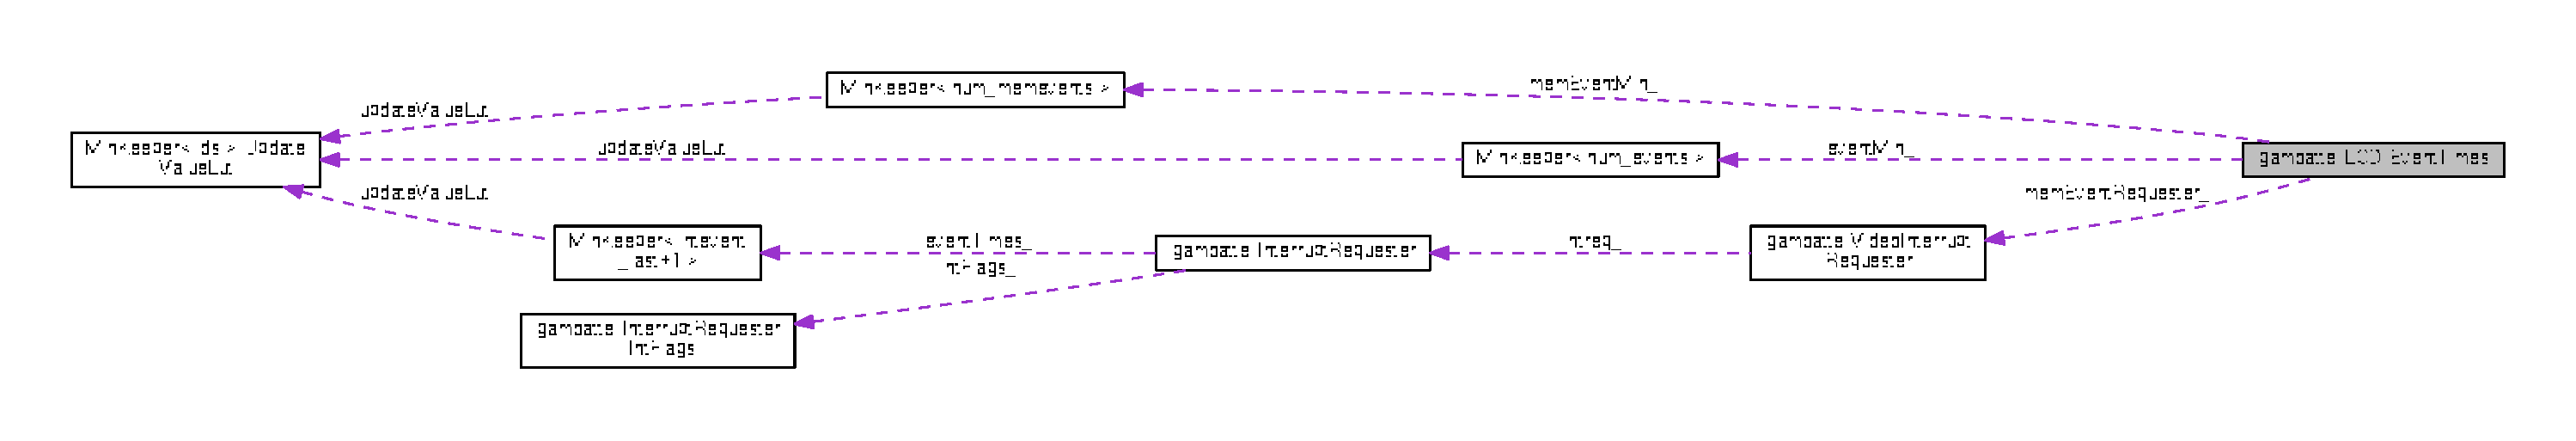
\includegraphics[width=350pt]{classgambatte_1_1LCD_1_1EventTimes__coll__graph}
\end{center}
\end{figure}
\subsection*{Public Member Functions}
\begin{DoxyCompactItemize}
\item 
\hyperlink{classgambatte_1_1LCD_1_1EventTimes_a1fa6d56defc84f65eb5d1a317091afc8}{Event\+Times} (\hyperlink{classgambatte_1_1VideoInterruptRequester}{Video\+Interrupt\+Requester} mem\+Event\+Requester)
\item 
\hyperlink{classgambatte_1_1LCD_a30ec19ea638b75c5c8972b2a1838b0c7}{Event} \hyperlink{classgambatte_1_1LCD_1_1EventTimes_a2822cb1d48ad650f8e5f433257991b85}{next\+Event} () const
\item 
unsigned \hyperlink{classgambatte_1_1LCD_1_1EventTimes_a0812df703759f4c4864e06fa6227a314}{next\+Event\+Time} () const
\item 
unsigned \hyperlink{classgambatte_1_1LCD_1_1EventTimes_a2e968a67987d0e7eb7afe188899e6699}{operator()} (\hyperlink{classgambatte_1_1LCD_a30ec19ea638b75c5c8972b2a1838b0c7}{Event} e) const
\item 
{\footnotesize template$<$Event e$>$ }\\void \hyperlink{classgambatte_1_1LCD_1_1EventTimes_a0bc5bcc9b1065d2603822e6db0a5eee8}{set} (unsigned time)
\item 
void \hyperlink{classgambatte_1_1LCD_1_1EventTimes_afa7238ae7fc6d48fdc710e4486dab4cd}{set} (\hyperlink{classgambatte_1_1LCD_a30ec19ea638b75c5c8972b2a1838b0c7}{Event} e, unsigned time)
\item 
\hyperlink{classgambatte_1_1LCD_a71147bde8c21c12e3cb7c70fcab81b76}{Mem\+Event} \hyperlink{classgambatte_1_1LCD_1_1EventTimes_a31230753beca7214709b10d6bf05aac1}{next\+Mem\+Event} () const
\item 
unsigned \hyperlink{classgambatte_1_1LCD_1_1EventTimes_aa9247fb79e7170125db355d380b4ec5d}{next\+Mem\+Event\+Time} () const
\item 
unsigned \hyperlink{classgambatte_1_1LCD_1_1EventTimes_acf5624c8f6b0971300d3e48b6580ec68}{operator()} (\hyperlink{classgambatte_1_1LCD_a71147bde8c21c12e3cb7c70fcab81b76}{Mem\+Event} e) const
\item 
{\footnotesize template$<$Mem\+Event e$>$ }\\void \hyperlink{classgambatte_1_1LCD_1_1EventTimes_a4f0607965b3cf9d9a4deb8ba19eb87de}{setm} (unsigned time)
\item 
void \hyperlink{classgambatte_1_1LCD_1_1EventTimes_ad11bf3927c4da8329f74cb605008d8ab}{set} (\hyperlink{classgambatte_1_1LCD_a71147bde8c21c12e3cb7c70fcab81b76}{Mem\+Event} e, unsigned time)
\item 
void \hyperlink{classgambatte_1_1LCD_1_1EventTimes_ad519fc1fbf6802530bb41956586e3551}{flag\+Irq} (unsigned bit)
\item 
void \hyperlink{classgambatte_1_1LCD_1_1EventTimes_a309beb0a36cdc41115c4c1322a6e174d}{flag\+Hdma\+Req} ()
\item 
void \hyperlink{classgambatte_1_1LCD_1_1EventTimes_a8393bd80f60b2a7d339c03bbbe06d53e}{load\+Or\+Save} (\hyperlink{classgambatte_1_1loadsave}{loadsave} \&\hyperlink{ppu_8cpp_a2f2eca6997ee7baf8901725ae074d45b}{state})
\end{DoxyCompactItemize}
\subsection*{Private Member Functions}
\begin{DoxyCompactItemize}
\item 
void \hyperlink{classgambatte_1_1LCD_1_1EventTimes_ab68dd9387d02b101f99adfffacb767f2}{set\+Mem\+Event} ()
\end{DoxyCompactItemize}
\subsection*{Private Attributes}
\begin{DoxyCompactItemize}
\item 
\hyperlink{classMinKeeper}{Min\+Keeper}$<$ \hyperlink{classgambatte_1_1LCD_a3f0d3ac1c0181cd4a083153515f43ec7a424a70f3d84f9af6281b1e034596f9cb}{num\+\_\+events} $>$ \hyperlink{classgambatte_1_1LCD_1_1EventTimes_a0a42dc4b789e866e6536313b44f9830d}{event\+Min\+\_\+}
\item 
\hyperlink{classMinKeeper}{Min\+Keeper}$<$ \hyperlink{classgambatte_1_1LCD_aa553646ad64f768ac0e781a5ccdde8a7a6f114e0d7de033bab11a657b9065edab}{num\+\_\+memevents} $>$ \hyperlink{classgambatte_1_1LCD_1_1EventTimes_afe898d5fd9e0c9df4d3516703059e8cb}{mem\+Event\+Min\+\_\+}
\item 
\hyperlink{classgambatte_1_1VideoInterruptRequester}{Video\+Interrupt\+Requester} \hyperlink{classgambatte_1_1LCD_1_1EventTimes_a3525ab9f34295420abdc8ca41de7829a}{mem\+Event\+Requester\+\_\+}
\end{DoxyCompactItemize}


\subsection{Constructor \& Destructor Documentation}
\mbox{\Hypertarget{classgambatte_1_1LCD_1_1EventTimes_a1fa6d56defc84f65eb5d1a317091afc8}\label{classgambatte_1_1LCD_1_1EventTimes_a1fa6d56defc84f65eb5d1a317091afc8}} 
\index{gambatte\+::\+L\+C\+D\+::\+Event\+Times@{gambatte\+::\+L\+C\+D\+::\+Event\+Times}!Event\+Times@{Event\+Times}}
\index{Event\+Times@{Event\+Times}!gambatte\+::\+L\+C\+D\+::\+Event\+Times@{gambatte\+::\+L\+C\+D\+::\+Event\+Times}}
\subsubsection{\texorpdfstring{Event\+Times()}{EventTimes()}}
{\footnotesize\ttfamily gambatte\+::\+L\+C\+D\+::\+Event\+Times\+::\+Event\+Times (\begin{DoxyParamCaption}\item[{\hyperlink{classgambatte_1_1VideoInterruptRequester}{Video\+Interrupt\+Requester}}]{mem\+Event\+Requester }\end{DoxyParamCaption})\hspace{0.3cm}{\ttfamily [inline]}, {\ttfamily [explicit]}}



\subsection{Member Function Documentation}
\mbox{\Hypertarget{classgambatte_1_1LCD_1_1EventTimes_a309beb0a36cdc41115c4c1322a6e174d}\label{classgambatte_1_1LCD_1_1EventTimes_a309beb0a36cdc41115c4c1322a6e174d}} 
\index{gambatte\+::\+L\+C\+D\+::\+Event\+Times@{gambatte\+::\+L\+C\+D\+::\+Event\+Times}!flag\+Hdma\+Req@{flag\+Hdma\+Req}}
\index{flag\+Hdma\+Req@{flag\+Hdma\+Req}!gambatte\+::\+L\+C\+D\+::\+Event\+Times@{gambatte\+::\+L\+C\+D\+::\+Event\+Times}}
\subsubsection{\texorpdfstring{flag\+Hdma\+Req()}{flagHdmaReq()}}
{\footnotesize\ttfamily void gambatte\+::\+L\+C\+D\+::\+Event\+Times\+::flag\+Hdma\+Req (\begin{DoxyParamCaption}{ }\end{DoxyParamCaption})\hspace{0.3cm}{\ttfamily [inline]}}

\mbox{\Hypertarget{classgambatte_1_1LCD_1_1EventTimes_ad519fc1fbf6802530bb41956586e3551}\label{classgambatte_1_1LCD_1_1EventTimes_ad519fc1fbf6802530bb41956586e3551}} 
\index{gambatte\+::\+L\+C\+D\+::\+Event\+Times@{gambatte\+::\+L\+C\+D\+::\+Event\+Times}!flag\+Irq@{flag\+Irq}}
\index{flag\+Irq@{flag\+Irq}!gambatte\+::\+L\+C\+D\+::\+Event\+Times@{gambatte\+::\+L\+C\+D\+::\+Event\+Times}}
\subsubsection{\texorpdfstring{flag\+Irq()}{flagIrq()}}
{\footnotesize\ttfamily void gambatte\+::\+L\+C\+D\+::\+Event\+Times\+::flag\+Irq (\begin{DoxyParamCaption}\item[{unsigned}]{bit }\end{DoxyParamCaption})\hspace{0.3cm}{\ttfamily [inline]}}

\mbox{\Hypertarget{classgambatte_1_1LCD_1_1EventTimes_a8393bd80f60b2a7d339c03bbbe06d53e}\label{classgambatte_1_1LCD_1_1EventTimes_a8393bd80f60b2a7d339c03bbbe06d53e}} 
\index{gambatte\+::\+L\+C\+D\+::\+Event\+Times@{gambatte\+::\+L\+C\+D\+::\+Event\+Times}!load\+Or\+Save@{load\+Or\+Save}}
\index{load\+Or\+Save@{load\+Or\+Save}!gambatte\+::\+L\+C\+D\+::\+Event\+Times@{gambatte\+::\+L\+C\+D\+::\+Event\+Times}}
\subsubsection{\texorpdfstring{load\+Or\+Save()}{loadOrSave()}}
{\footnotesize\ttfamily void gambatte\+::\+L\+C\+D\+::\+Event\+Times\+::load\+Or\+Save (\begin{DoxyParamCaption}\item[{\hyperlink{classgambatte_1_1loadsave}{loadsave} \&}]{state }\end{DoxyParamCaption})\hspace{0.3cm}{\ttfamily [inline]}}

\mbox{\Hypertarget{classgambatte_1_1LCD_1_1EventTimes_a2822cb1d48ad650f8e5f433257991b85}\label{classgambatte_1_1LCD_1_1EventTimes_a2822cb1d48ad650f8e5f433257991b85}} 
\index{gambatte\+::\+L\+C\+D\+::\+Event\+Times@{gambatte\+::\+L\+C\+D\+::\+Event\+Times}!next\+Event@{next\+Event}}
\index{next\+Event@{next\+Event}!gambatte\+::\+L\+C\+D\+::\+Event\+Times@{gambatte\+::\+L\+C\+D\+::\+Event\+Times}}
\subsubsection{\texorpdfstring{next\+Event()}{nextEvent()}}
{\footnotesize\ttfamily \hyperlink{classgambatte_1_1LCD_a30ec19ea638b75c5c8972b2a1838b0c7}{Event} gambatte\+::\+L\+C\+D\+::\+Event\+Times\+::next\+Event (\begin{DoxyParamCaption}{ }\end{DoxyParamCaption}) const\hspace{0.3cm}{\ttfamily [inline]}}

\mbox{\Hypertarget{classgambatte_1_1LCD_1_1EventTimes_a0812df703759f4c4864e06fa6227a314}\label{classgambatte_1_1LCD_1_1EventTimes_a0812df703759f4c4864e06fa6227a314}} 
\index{gambatte\+::\+L\+C\+D\+::\+Event\+Times@{gambatte\+::\+L\+C\+D\+::\+Event\+Times}!next\+Event\+Time@{next\+Event\+Time}}
\index{next\+Event\+Time@{next\+Event\+Time}!gambatte\+::\+L\+C\+D\+::\+Event\+Times@{gambatte\+::\+L\+C\+D\+::\+Event\+Times}}
\subsubsection{\texorpdfstring{next\+Event\+Time()}{nextEventTime()}}
{\footnotesize\ttfamily unsigned gambatte\+::\+L\+C\+D\+::\+Event\+Times\+::next\+Event\+Time (\begin{DoxyParamCaption}{ }\end{DoxyParamCaption}) const\hspace{0.3cm}{\ttfamily [inline]}}

\mbox{\Hypertarget{classgambatte_1_1LCD_1_1EventTimes_a31230753beca7214709b10d6bf05aac1}\label{classgambatte_1_1LCD_1_1EventTimes_a31230753beca7214709b10d6bf05aac1}} 
\index{gambatte\+::\+L\+C\+D\+::\+Event\+Times@{gambatte\+::\+L\+C\+D\+::\+Event\+Times}!next\+Mem\+Event@{next\+Mem\+Event}}
\index{next\+Mem\+Event@{next\+Mem\+Event}!gambatte\+::\+L\+C\+D\+::\+Event\+Times@{gambatte\+::\+L\+C\+D\+::\+Event\+Times}}
\subsubsection{\texorpdfstring{next\+Mem\+Event()}{nextMemEvent()}}
{\footnotesize\ttfamily \hyperlink{classgambatte_1_1LCD_a71147bde8c21c12e3cb7c70fcab81b76}{Mem\+Event} gambatte\+::\+L\+C\+D\+::\+Event\+Times\+::next\+Mem\+Event (\begin{DoxyParamCaption}{ }\end{DoxyParamCaption}) const\hspace{0.3cm}{\ttfamily [inline]}}

\mbox{\Hypertarget{classgambatte_1_1LCD_1_1EventTimes_aa9247fb79e7170125db355d380b4ec5d}\label{classgambatte_1_1LCD_1_1EventTimes_aa9247fb79e7170125db355d380b4ec5d}} 
\index{gambatte\+::\+L\+C\+D\+::\+Event\+Times@{gambatte\+::\+L\+C\+D\+::\+Event\+Times}!next\+Mem\+Event\+Time@{next\+Mem\+Event\+Time}}
\index{next\+Mem\+Event\+Time@{next\+Mem\+Event\+Time}!gambatte\+::\+L\+C\+D\+::\+Event\+Times@{gambatte\+::\+L\+C\+D\+::\+Event\+Times}}
\subsubsection{\texorpdfstring{next\+Mem\+Event\+Time()}{nextMemEventTime()}}
{\footnotesize\ttfamily unsigned gambatte\+::\+L\+C\+D\+::\+Event\+Times\+::next\+Mem\+Event\+Time (\begin{DoxyParamCaption}{ }\end{DoxyParamCaption}) const\hspace{0.3cm}{\ttfamily [inline]}}

\mbox{\Hypertarget{classgambatte_1_1LCD_1_1EventTimes_a2e968a67987d0e7eb7afe188899e6699}\label{classgambatte_1_1LCD_1_1EventTimes_a2e968a67987d0e7eb7afe188899e6699}} 
\index{gambatte\+::\+L\+C\+D\+::\+Event\+Times@{gambatte\+::\+L\+C\+D\+::\+Event\+Times}!operator()@{operator()}}
\index{operator()@{operator()}!gambatte\+::\+L\+C\+D\+::\+Event\+Times@{gambatte\+::\+L\+C\+D\+::\+Event\+Times}}
\subsubsection{\texorpdfstring{operator()()}{operator()()}\hspace{0.1cm}{\footnotesize\ttfamily [1/2]}}
{\footnotesize\ttfamily unsigned gambatte\+::\+L\+C\+D\+::\+Event\+Times\+::operator() (\begin{DoxyParamCaption}\item[{\hyperlink{classgambatte_1_1LCD_a30ec19ea638b75c5c8972b2a1838b0c7}{Event}}]{e }\end{DoxyParamCaption}) const\hspace{0.3cm}{\ttfamily [inline]}}

\mbox{\Hypertarget{classgambatte_1_1LCD_1_1EventTimes_acf5624c8f6b0971300d3e48b6580ec68}\label{classgambatte_1_1LCD_1_1EventTimes_acf5624c8f6b0971300d3e48b6580ec68}} 
\index{gambatte\+::\+L\+C\+D\+::\+Event\+Times@{gambatte\+::\+L\+C\+D\+::\+Event\+Times}!operator()@{operator()}}
\index{operator()@{operator()}!gambatte\+::\+L\+C\+D\+::\+Event\+Times@{gambatte\+::\+L\+C\+D\+::\+Event\+Times}}
\subsubsection{\texorpdfstring{operator()()}{operator()()}\hspace{0.1cm}{\footnotesize\ttfamily [2/2]}}
{\footnotesize\ttfamily unsigned gambatte\+::\+L\+C\+D\+::\+Event\+Times\+::operator() (\begin{DoxyParamCaption}\item[{\hyperlink{classgambatte_1_1LCD_a71147bde8c21c12e3cb7c70fcab81b76}{Mem\+Event}}]{e }\end{DoxyParamCaption}) const\hspace{0.3cm}{\ttfamily [inline]}}

\mbox{\Hypertarget{classgambatte_1_1LCD_1_1EventTimes_a0bc5bcc9b1065d2603822e6db0a5eee8}\label{classgambatte_1_1LCD_1_1EventTimes_a0bc5bcc9b1065d2603822e6db0a5eee8}} 
\index{gambatte\+::\+L\+C\+D\+::\+Event\+Times@{gambatte\+::\+L\+C\+D\+::\+Event\+Times}!set@{set}}
\index{set@{set}!gambatte\+::\+L\+C\+D\+::\+Event\+Times@{gambatte\+::\+L\+C\+D\+::\+Event\+Times}}
\subsubsection{\texorpdfstring{set()}{set()}\hspace{0.1cm}{\footnotesize\ttfamily [1/3]}}
{\footnotesize\ttfamily template$<$Event e$>$ \\
void gambatte\+::\+L\+C\+D\+::\+Event\+Times\+::set (\begin{DoxyParamCaption}\item[{unsigned}]{time }\end{DoxyParamCaption})\hspace{0.3cm}{\ttfamily [inline]}}

\mbox{\Hypertarget{classgambatte_1_1LCD_1_1EventTimes_afa7238ae7fc6d48fdc710e4486dab4cd}\label{classgambatte_1_1LCD_1_1EventTimes_afa7238ae7fc6d48fdc710e4486dab4cd}} 
\index{gambatte\+::\+L\+C\+D\+::\+Event\+Times@{gambatte\+::\+L\+C\+D\+::\+Event\+Times}!set@{set}}
\index{set@{set}!gambatte\+::\+L\+C\+D\+::\+Event\+Times@{gambatte\+::\+L\+C\+D\+::\+Event\+Times}}
\subsubsection{\texorpdfstring{set()}{set()}\hspace{0.1cm}{\footnotesize\ttfamily [2/3]}}
{\footnotesize\ttfamily void gambatte\+::\+L\+C\+D\+::\+Event\+Times\+::set (\begin{DoxyParamCaption}\item[{\hyperlink{classgambatte_1_1LCD_a30ec19ea638b75c5c8972b2a1838b0c7}{Event}}]{e,  }\item[{unsigned}]{time }\end{DoxyParamCaption})\hspace{0.3cm}{\ttfamily [inline]}}

\mbox{\Hypertarget{classgambatte_1_1LCD_1_1EventTimes_ad11bf3927c4da8329f74cb605008d8ab}\label{classgambatte_1_1LCD_1_1EventTimes_ad11bf3927c4da8329f74cb605008d8ab}} 
\index{gambatte\+::\+L\+C\+D\+::\+Event\+Times@{gambatte\+::\+L\+C\+D\+::\+Event\+Times}!set@{set}}
\index{set@{set}!gambatte\+::\+L\+C\+D\+::\+Event\+Times@{gambatte\+::\+L\+C\+D\+::\+Event\+Times}}
\subsubsection{\texorpdfstring{set()}{set()}\hspace{0.1cm}{\footnotesize\ttfamily [3/3]}}
{\footnotesize\ttfamily void gambatte\+::\+L\+C\+D\+::\+Event\+Times\+::set (\begin{DoxyParamCaption}\item[{\hyperlink{classgambatte_1_1LCD_a71147bde8c21c12e3cb7c70fcab81b76}{Mem\+Event}}]{e,  }\item[{unsigned}]{time }\end{DoxyParamCaption})\hspace{0.3cm}{\ttfamily [inline]}}

\mbox{\Hypertarget{classgambatte_1_1LCD_1_1EventTimes_a4f0607965b3cf9d9a4deb8ba19eb87de}\label{classgambatte_1_1LCD_1_1EventTimes_a4f0607965b3cf9d9a4deb8ba19eb87de}} 
\index{gambatte\+::\+L\+C\+D\+::\+Event\+Times@{gambatte\+::\+L\+C\+D\+::\+Event\+Times}!setm@{setm}}
\index{setm@{setm}!gambatte\+::\+L\+C\+D\+::\+Event\+Times@{gambatte\+::\+L\+C\+D\+::\+Event\+Times}}
\subsubsection{\texorpdfstring{setm()}{setm()}}
{\footnotesize\ttfamily template$<$Mem\+Event e$>$ \\
void gambatte\+::\+L\+C\+D\+::\+Event\+Times\+::setm (\begin{DoxyParamCaption}\item[{unsigned}]{time }\end{DoxyParamCaption})\hspace{0.3cm}{\ttfamily [inline]}}

\mbox{\Hypertarget{classgambatte_1_1LCD_1_1EventTimes_ab68dd9387d02b101f99adfffacb767f2}\label{classgambatte_1_1LCD_1_1EventTimes_ab68dd9387d02b101f99adfffacb767f2}} 
\index{gambatte\+::\+L\+C\+D\+::\+Event\+Times@{gambatte\+::\+L\+C\+D\+::\+Event\+Times}!set\+Mem\+Event@{set\+Mem\+Event}}
\index{set\+Mem\+Event@{set\+Mem\+Event}!gambatte\+::\+L\+C\+D\+::\+Event\+Times@{gambatte\+::\+L\+C\+D\+::\+Event\+Times}}
\subsubsection{\texorpdfstring{set\+Mem\+Event()}{setMemEvent()}}
{\footnotesize\ttfamily void gambatte\+::\+L\+C\+D\+::\+Event\+Times\+::set\+Mem\+Event (\begin{DoxyParamCaption}{ }\end{DoxyParamCaption})\hspace{0.3cm}{\ttfamily [inline]}, {\ttfamily [private]}}



\subsection{Member Data Documentation}
\mbox{\Hypertarget{classgambatte_1_1LCD_1_1EventTimes_a0a42dc4b789e866e6536313b44f9830d}\label{classgambatte_1_1LCD_1_1EventTimes_a0a42dc4b789e866e6536313b44f9830d}} 
\index{gambatte\+::\+L\+C\+D\+::\+Event\+Times@{gambatte\+::\+L\+C\+D\+::\+Event\+Times}!event\+Min\+\_\+@{event\+Min\+\_\+}}
\index{event\+Min\+\_\+@{event\+Min\+\_\+}!gambatte\+::\+L\+C\+D\+::\+Event\+Times@{gambatte\+::\+L\+C\+D\+::\+Event\+Times}}
\subsubsection{\texorpdfstring{event\+Min\+\_\+}{eventMin\_}}
{\footnotesize\ttfamily \hyperlink{classMinKeeper}{Min\+Keeper}$<$\hyperlink{classgambatte_1_1LCD_a3f0d3ac1c0181cd4a083153515f43ec7a424a70f3d84f9af6281b1e034596f9cb}{num\+\_\+events}$>$ gambatte\+::\+L\+C\+D\+::\+Event\+Times\+::event\+Min\+\_\+\hspace{0.3cm}{\ttfamily [private]}}

\mbox{\Hypertarget{classgambatte_1_1LCD_1_1EventTimes_afe898d5fd9e0c9df4d3516703059e8cb}\label{classgambatte_1_1LCD_1_1EventTimes_afe898d5fd9e0c9df4d3516703059e8cb}} 
\index{gambatte\+::\+L\+C\+D\+::\+Event\+Times@{gambatte\+::\+L\+C\+D\+::\+Event\+Times}!mem\+Event\+Min\+\_\+@{mem\+Event\+Min\+\_\+}}
\index{mem\+Event\+Min\+\_\+@{mem\+Event\+Min\+\_\+}!gambatte\+::\+L\+C\+D\+::\+Event\+Times@{gambatte\+::\+L\+C\+D\+::\+Event\+Times}}
\subsubsection{\texorpdfstring{mem\+Event\+Min\+\_\+}{memEventMin\_}}
{\footnotesize\ttfamily \hyperlink{classMinKeeper}{Min\+Keeper}$<$\hyperlink{classgambatte_1_1LCD_aa553646ad64f768ac0e781a5ccdde8a7a6f114e0d7de033bab11a657b9065edab}{num\+\_\+memevents}$>$ gambatte\+::\+L\+C\+D\+::\+Event\+Times\+::mem\+Event\+Min\+\_\+\hspace{0.3cm}{\ttfamily [private]}}

\mbox{\Hypertarget{classgambatte_1_1LCD_1_1EventTimes_a3525ab9f34295420abdc8ca41de7829a}\label{classgambatte_1_1LCD_1_1EventTimes_a3525ab9f34295420abdc8ca41de7829a}} 
\index{gambatte\+::\+L\+C\+D\+::\+Event\+Times@{gambatte\+::\+L\+C\+D\+::\+Event\+Times}!mem\+Event\+Requester\+\_\+@{mem\+Event\+Requester\+\_\+}}
\index{mem\+Event\+Requester\+\_\+@{mem\+Event\+Requester\+\_\+}!gambatte\+::\+L\+C\+D\+::\+Event\+Times@{gambatte\+::\+L\+C\+D\+::\+Event\+Times}}
\subsubsection{\texorpdfstring{mem\+Event\+Requester\+\_\+}{memEventRequester\_}}
{\footnotesize\ttfamily \hyperlink{classgambatte_1_1VideoInterruptRequester}{Video\+Interrupt\+Requester} gambatte\+::\+L\+C\+D\+::\+Event\+Times\+::mem\+Event\+Requester\+\_\+\hspace{0.3cm}{\ttfamily [private]}}



The documentation for this class was generated from the following file\+:\begin{DoxyCompactItemize}
\item 
src/\hyperlink{video_8h}{video.\+h}\end{DoxyCompactItemize}

\hypertarget{classgambatte_1_1File}{}\section{gambatte\+:\+:File Class Reference}
\label{classgambatte_1_1File}\index{gambatte\+::\+File@{gambatte\+::\+File}}


{\ttfamily \#include $<$file.\+h$>$}



Inheritance diagram for gambatte\+:\+:File\+:\nopagebreak
\begin{figure}[H]
\begin{center}
\leavevmode
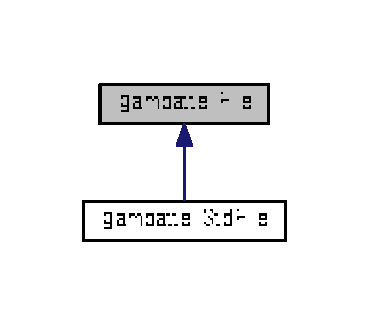
\includegraphics[width=177pt]{classgambatte_1_1File__inherit__graph}
\end{center}
\end{figure}
\subsection*{Public Member Functions}
\begin{DoxyCompactItemize}
\item 
virtual \hyperlink{classgambatte_1_1File_a02609e94947a742b6225b2f2fc828d46}{$\sim$\+File} ()
\item 
virtual void \hyperlink{classgambatte_1_1File_a37e873832be84757982d7a03662dfb95}{rewind} ()=0
\item 
virtual std\+::size\+\_\+t \hyperlink{classgambatte_1_1File_a589f615d436595eb97cbb9b9dc36632e}{size} () const =0
\item 
virtual void \hyperlink{classgambatte_1_1File_a58a6f97f55c93d15c9aa067d2a6db123}{read} (char $\ast$buffer, std\+::size\+\_\+t amount)=0
\item 
virtual bool \hyperlink{classgambatte_1_1File_ac4e6a7055cd91176c9fb3e9215370c51}{fail} () const =0
\end{DoxyCompactItemize}


\subsection{Constructor \& Destructor Documentation}
\mbox{\Hypertarget{classgambatte_1_1File_a02609e94947a742b6225b2f2fc828d46}\label{classgambatte_1_1File_a02609e94947a742b6225b2f2fc828d46}} 
\index{gambatte\+::\+File@{gambatte\+::\+File}!````~File@{$\sim$\+File}}
\index{````~File@{$\sim$\+File}!gambatte\+::\+File@{gambatte\+::\+File}}
\subsubsection{\texorpdfstring{$\sim$\+File()}{~File()}}
{\footnotesize\ttfamily virtual gambatte\+::\+File\+::$\sim$\+File (\begin{DoxyParamCaption}{ }\end{DoxyParamCaption})\hspace{0.3cm}{\ttfamily [inline]}, {\ttfamily [virtual]}}



\subsection{Member Function Documentation}
\mbox{\Hypertarget{classgambatte_1_1File_ac4e6a7055cd91176c9fb3e9215370c51}\label{classgambatte_1_1File_ac4e6a7055cd91176c9fb3e9215370c51}} 
\index{gambatte\+::\+File@{gambatte\+::\+File}!fail@{fail}}
\index{fail@{fail}!gambatte\+::\+File@{gambatte\+::\+File}}
\subsubsection{\texorpdfstring{fail()}{fail()}}
{\footnotesize\ttfamily virtual bool gambatte\+::\+File\+::fail (\begin{DoxyParamCaption}{ }\end{DoxyParamCaption}) const\hspace{0.3cm}{\ttfamily [pure virtual]}}



Implemented in \hyperlink{classgambatte_1_1StdFile_aa4f8f0f2854e3b11a71cb3d3109908eb}{gambatte\+::\+Std\+File}.

\mbox{\Hypertarget{classgambatte_1_1File_a58a6f97f55c93d15c9aa067d2a6db123}\label{classgambatte_1_1File_a58a6f97f55c93d15c9aa067d2a6db123}} 
\index{gambatte\+::\+File@{gambatte\+::\+File}!read@{read}}
\index{read@{read}!gambatte\+::\+File@{gambatte\+::\+File}}
\subsubsection{\texorpdfstring{read()}{read()}}
{\footnotesize\ttfamily virtual void gambatte\+::\+File\+::read (\begin{DoxyParamCaption}\item[{char $\ast$}]{buffer,  }\item[{std\+::size\+\_\+t}]{amount }\end{DoxyParamCaption})\hspace{0.3cm}{\ttfamily [pure virtual]}}



Implemented in \hyperlink{classgambatte_1_1StdFile_a8c9c0994af30457e852ee887c1f9b38c}{gambatte\+::\+Std\+File}.

\mbox{\Hypertarget{classgambatte_1_1File_a37e873832be84757982d7a03662dfb95}\label{classgambatte_1_1File_a37e873832be84757982d7a03662dfb95}} 
\index{gambatte\+::\+File@{gambatte\+::\+File}!rewind@{rewind}}
\index{rewind@{rewind}!gambatte\+::\+File@{gambatte\+::\+File}}
\subsubsection{\texorpdfstring{rewind()}{rewind()}}
{\footnotesize\ttfamily virtual void gambatte\+::\+File\+::rewind (\begin{DoxyParamCaption}{ }\end{DoxyParamCaption})\hspace{0.3cm}{\ttfamily [pure virtual]}}



Implemented in \hyperlink{classgambatte_1_1StdFile_aa9f4ffbac979a4bf7607992eff78f469}{gambatte\+::\+Std\+File}.

\mbox{\Hypertarget{classgambatte_1_1File_a589f615d436595eb97cbb9b9dc36632e}\label{classgambatte_1_1File_a589f615d436595eb97cbb9b9dc36632e}} 
\index{gambatte\+::\+File@{gambatte\+::\+File}!size@{size}}
\index{size@{size}!gambatte\+::\+File@{gambatte\+::\+File}}
\subsubsection{\texorpdfstring{size()}{size()}}
{\footnotesize\ttfamily virtual std\+::size\+\_\+t gambatte\+::\+File\+::size (\begin{DoxyParamCaption}{ }\end{DoxyParamCaption}) const\hspace{0.3cm}{\ttfamily [pure virtual]}}



Implemented in \hyperlink{classgambatte_1_1StdFile_aac486706e2f657b7396757ee9f8e7352}{gambatte\+::\+Std\+File}.



The documentation for this class was generated from the following file\+:\begin{DoxyCompactItemize}
\item 
src/file/\hyperlink{file_8h}{file.\+h}\end{DoxyCompactItemize}

\hypertarget{structfile__in__zip__read__info__s}{}\section{file\+\_\+in\+\_\+zip\+\_\+read\+\_\+info\+\_\+s Struct Reference}
\label{structfile__in__zip__read__info__s}\index{file\+\_\+in\+\_\+zip\+\_\+read\+\_\+info\+\_\+s@{file\+\_\+in\+\_\+zip\+\_\+read\+\_\+info\+\_\+s}}


Collaboration diagram for file\+\_\+in\+\_\+zip\+\_\+read\+\_\+info\+\_\+s\+:\nopagebreak
\begin{figure}[H]
\begin{center}
\leavevmode
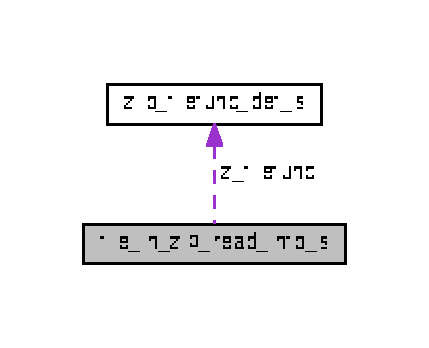
\includegraphics[width=206pt]{structfile__in__zip__read__info__s__coll__graph}
\end{center}
\end{figure}
\subsection*{Public Attributes}
\begin{DoxyCompactItemize}
\item 
char $\ast$ \hyperlink{structfile__in__zip__read__info__s_a6310a19e33ac2cf3280aa74199cbd89b}{read\+\_\+buffer}
\item 
z\+\_\+stream \hyperlink{structfile__in__zip__read__info__s_a6973c6240c02a1c8e014d6078bb2bbfc}{stream}
\item 
\hyperlink{ioapi_8h_a50e9e9d5c30e481de822ad68fe537986}{u\+Long} \hyperlink{structfile__in__zip__read__info__s_a01d6195d7977bec4db506cdbee9b8a13}{pos\+\_\+in\+\_\+zipfile}
\item 
\hyperlink{ioapi_8h_a50e9e9d5c30e481de822ad68fe537986}{u\+Long} \hyperlink{structfile__in__zip__read__info__s_a8f2d03c24a7b1058288606687eb6d448}{stream\+\_\+initialised}
\item 
\hyperlink{ioapi_8h_a50e9e9d5c30e481de822ad68fe537986}{u\+Long} \hyperlink{structfile__in__zip__read__info__s_a8e3a240c367e7d6d199859b1b311128c}{offset\+\_\+local\+\_\+extrafield}
\item 
u\+Int \hyperlink{structfile__in__zip__read__info__s_a9abdc9b3f3d500d894a635cc9e956180}{size\+\_\+local\+\_\+extrafield}
\item 
\hyperlink{ioapi_8h_a50e9e9d5c30e481de822ad68fe537986}{u\+Long} \hyperlink{structfile__in__zip__read__info__s_aa07cf3d7d5d68e9537ffe99499d7db6f}{pos\+\_\+local\+\_\+extrafield}
\item 
\hyperlink{ioapi_8h_a50e9e9d5c30e481de822ad68fe537986}{u\+Long} \hyperlink{structfile__in__zip__read__info__s_a9d7e4dc6f312fb59bf8e60fb952f4d68}{crc32}
\item 
\hyperlink{ioapi_8h_a50e9e9d5c30e481de822ad68fe537986}{u\+Long} \hyperlink{structfile__in__zip__read__info__s_a6120c521be40e8ba530249f0c766ab9d}{crc32\+\_\+wait}
\item 
\hyperlink{ioapi_8h_a50e9e9d5c30e481de822ad68fe537986}{u\+Long} \hyperlink{structfile__in__zip__read__info__s_a4c7b8e6502f7195feefd676dff0bb494}{rest\+\_\+read\+\_\+compressed}
\item 
\hyperlink{ioapi_8h_a50e9e9d5c30e481de822ad68fe537986}{u\+Long} \hyperlink{structfile__in__zip__read__info__s_a8e3801645cfa5bfd147fd8d037fcf9a5}{rest\+\_\+read\+\_\+uncompressed}
\item 
\hyperlink{ioapi_8h_a269f2bded66a7ee4052a60025afebd7e}{zlib\+\_\+filefunc\+\_\+def} \hyperlink{structfile__in__zip__read__info__s_a5eae7e8fffe8d7e9e7271ce2206283e7}{z\+\_\+filefunc}
\item 
\hyperlink{ioapi_8h_a39ab6d73c1cd44bc17064c2dcbb3e753}{voidpf} \hyperlink{structfile__in__zip__read__info__s_ab0b66746406599abe4528b7b48961bba}{filestream}
\item 
\hyperlink{ioapi_8h_a50e9e9d5c30e481de822ad68fe537986}{u\+Long} \hyperlink{structfile__in__zip__read__info__s_a86cbaa96568192cae9ab9cd606963fdb}{compression\+\_\+method}
\item 
\hyperlink{ioapi_8h_a50e9e9d5c30e481de822ad68fe537986}{u\+Long} \hyperlink{structfile__in__zip__read__info__s_a52c8e657a1238a3b9fa87b4167d9b7a3}{byte\+\_\+before\+\_\+the\+\_\+zipfile}
\item 
\hyperlink{ioapi_8h_a787fa3cf048117ba7123753c1e74fcd6}{int} \hyperlink{structfile__in__zip__read__info__s_aec0649000ce059ef1262b5a5be1641fe}{raw}
\end{DoxyCompactItemize}


\subsection{Member Data Documentation}
\mbox{\Hypertarget{structfile__in__zip__read__info__s_a52c8e657a1238a3b9fa87b4167d9b7a3}\label{structfile__in__zip__read__info__s_a52c8e657a1238a3b9fa87b4167d9b7a3}} 
\index{file\+\_\+in\+\_\+zip\+\_\+read\+\_\+info\+\_\+s@{file\+\_\+in\+\_\+zip\+\_\+read\+\_\+info\+\_\+s}!byte\+\_\+before\+\_\+the\+\_\+zipfile@{byte\+\_\+before\+\_\+the\+\_\+zipfile}}
\index{byte\+\_\+before\+\_\+the\+\_\+zipfile@{byte\+\_\+before\+\_\+the\+\_\+zipfile}!file\+\_\+in\+\_\+zip\+\_\+read\+\_\+info\+\_\+s@{file\+\_\+in\+\_\+zip\+\_\+read\+\_\+info\+\_\+s}}
\subsubsection{\texorpdfstring{byte\+\_\+before\+\_\+the\+\_\+zipfile}{byte\_before\_the\_zipfile}}
{\footnotesize\ttfamily \hyperlink{ioapi_8h_a50e9e9d5c30e481de822ad68fe537986}{u\+Long} file\+\_\+in\+\_\+zip\+\_\+read\+\_\+info\+\_\+s\+::byte\+\_\+before\+\_\+the\+\_\+zipfile}

\mbox{\Hypertarget{structfile__in__zip__read__info__s_a86cbaa96568192cae9ab9cd606963fdb}\label{structfile__in__zip__read__info__s_a86cbaa96568192cae9ab9cd606963fdb}} 
\index{file\+\_\+in\+\_\+zip\+\_\+read\+\_\+info\+\_\+s@{file\+\_\+in\+\_\+zip\+\_\+read\+\_\+info\+\_\+s}!compression\+\_\+method@{compression\+\_\+method}}
\index{compression\+\_\+method@{compression\+\_\+method}!file\+\_\+in\+\_\+zip\+\_\+read\+\_\+info\+\_\+s@{file\+\_\+in\+\_\+zip\+\_\+read\+\_\+info\+\_\+s}}
\subsubsection{\texorpdfstring{compression\+\_\+method}{compression\_method}}
{\footnotesize\ttfamily \hyperlink{ioapi_8h_a50e9e9d5c30e481de822ad68fe537986}{u\+Long} file\+\_\+in\+\_\+zip\+\_\+read\+\_\+info\+\_\+s\+::compression\+\_\+method}

\mbox{\Hypertarget{structfile__in__zip__read__info__s_a9d7e4dc6f312fb59bf8e60fb952f4d68}\label{structfile__in__zip__read__info__s_a9d7e4dc6f312fb59bf8e60fb952f4d68}} 
\index{file\+\_\+in\+\_\+zip\+\_\+read\+\_\+info\+\_\+s@{file\+\_\+in\+\_\+zip\+\_\+read\+\_\+info\+\_\+s}!crc32@{crc32}}
\index{crc32@{crc32}!file\+\_\+in\+\_\+zip\+\_\+read\+\_\+info\+\_\+s@{file\+\_\+in\+\_\+zip\+\_\+read\+\_\+info\+\_\+s}}
\subsubsection{\texorpdfstring{crc32}{crc32}}
{\footnotesize\ttfamily \hyperlink{ioapi_8h_a50e9e9d5c30e481de822ad68fe537986}{u\+Long} file\+\_\+in\+\_\+zip\+\_\+read\+\_\+info\+\_\+s\+::crc32}

\mbox{\Hypertarget{structfile__in__zip__read__info__s_a6120c521be40e8ba530249f0c766ab9d}\label{structfile__in__zip__read__info__s_a6120c521be40e8ba530249f0c766ab9d}} 
\index{file\+\_\+in\+\_\+zip\+\_\+read\+\_\+info\+\_\+s@{file\+\_\+in\+\_\+zip\+\_\+read\+\_\+info\+\_\+s}!crc32\+\_\+wait@{crc32\+\_\+wait}}
\index{crc32\+\_\+wait@{crc32\+\_\+wait}!file\+\_\+in\+\_\+zip\+\_\+read\+\_\+info\+\_\+s@{file\+\_\+in\+\_\+zip\+\_\+read\+\_\+info\+\_\+s}}
\subsubsection{\texorpdfstring{crc32\+\_\+wait}{crc32\_wait}}
{\footnotesize\ttfamily \hyperlink{ioapi_8h_a50e9e9d5c30e481de822ad68fe537986}{u\+Long} file\+\_\+in\+\_\+zip\+\_\+read\+\_\+info\+\_\+s\+::crc32\+\_\+wait}

\mbox{\Hypertarget{structfile__in__zip__read__info__s_ab0b66746406599abe4528b7b48961bba}\label{structfile__in__zip__read__info__s_ab0b66746406599abe4528b7b48961bba}} 
\index{file\+\_\+in\+\_\+zip\+\_\+read\+\_\+info\+\_\+s@{file\+\_\+in\+\_\+zip\+\_\+read\+\_\+info\+\_\+s}!filestream@{filestream}}
\index{filestream@{filestream}!file\+\_\+in\+\_\+zip\+\_\+read\+\_\+info\+\_\+s@{file\+\_\+in\+\_\+zip\+\_\+read\+\_\+info\+\_\+s}}
\subsubsection{\texorpdfstring{filestream}{filestream}}
{\footnotesize\ttfamily \hyperlink{ioapi_8h_a39ab6d73c1cd44bc17064c2dcbb3e753}{voidpf} file\+\_\+in\+\_\+zip\+\_\+read\+\_\+info\+\_\+s\+::filestream}

\mbox{\Hypertarget{structfile__in__zip__read__info__s_a8e3a240c367e7d6d199859b1b311128c}\label{structfile__in__zip__read__info__s_a8e3a240c367e7d6d199859b1b311128c}} 
\index{file\+\_\+in\+\_\+zip\+\_\+read\+\_\+info\+\_\+s@{file\+\_\+in\+\_\+zip\+\_\+read\+\_\+info\+\_\+s}!offset\+\_\+local\+\_\+extrafield@{offset\+\_\+local\+\_\+extrafield}}
\index{offset\+\_\+local\+\_\+extrafield@{offset\+\_\+local\+\_\+extrafield}!file\+\_\+in\+\_\+zip\+\_\+read\+\_\+info\+\_\+s@{file\+\_\+in\+\_\+zip\+\_\+read\+\_\+info\+\_\+s}}
\subsubsection{\texorpdfstring{offset\+\_\+local\+\_\+extrafield}{offset\_local\_extrafield}}
{\footnotesize\ttfamily \hyperlink{ioapi_8h_a50e9e9d5c30e481de822ad68fe537986}{u\+Long} file\+\_\+in\+\_\+zip\+\_\+read\+\_\+info\+\_\+s\+::offset\+\_\+local\+\_\+extrafield}

\mbox{\Hypertarget{structfile__in__zip__read__info__s_a01d6195d7977bec4db506cdbee9b8a13}\label{structfile__in__zip__read__info__s_a01d6195d7977bec4db506cdbee9b8a13}} 
\index{file\+\_\+in\+\_\+zip\+\_\+read\+\_\+info\+\_\+s@{file\+\_\+in\+\_\+zip\+\_\+read\+\_\+info\+\_\+s}!pos\+\_\+in\+\_\+zipfile@{pos\+\_\+in\+\_\+zipfile}}
\index{pos\+\_\+in\+\_\+zipfile@{pos\+\_\+in\+\_\+zipfile}!file\+\_\+in\+\_\+zip\+\_\+read\+\_\+info\+\_\+s@{file\+\_\+in\+\_\+zip\+\_\+read\+\_\+info\+\_\+s}}
\subsubsection{\texorpdfstring{pos\+\_\+in\+\_\+zipfile}{pos\_in\_zipfile}}
{\footnotesize\ttfamily \hyperlink{ioapi_8h_a50e9e9d5c30e481de822ad68fe537986}{u\+Long} file\+\_\+in\+\_\+zip\+\_\+read\+\_\+info\+\_\+s\+::pos\+\_\+in\+\_\+zipfile}

\mbox{\Hypertarget{structfile__in__zip__read__info__s_aa07cf3d7d5d68e9537ffe99499d7db6f}\label{structfile__in__zip__read__info__s_aa07cf3d7d5d68e9537ffe99499d7db6f}} 
\index{file\+\_\+in\+\_\+zip\+\_\+read\+\_\+info\+\_\+s@{file\+\_\+in\+\_\+zip\+\_\+read\+\_\+info\+\_\+s}!pos\+\_\+local\+\_\+extrafield@{pos\+\_\+local\+\_\+extrafield}}
\index{pos\+\_\+local\+\_\+extrafield@{pos\+\_\+local\+\_\+extrafield}!file\+\_\+in\+\_\+zip\+\_\+read\+\_\+info\+\_\+s@{file\+\_\+in\+\_\+zip\+\_\+read\+\_\+info\+\_\+s}}
\subsubsection{\texorpdfstring{pos\+\_\+local\+\_\+extrafield}{pos\_local\_extrafield}}
{\footnotesize\ttfamily \hyperlink{ioapi_8h_a50e9e9d5c30e481de822ad68fe537986}{u\+Long} file\+\_\+in\+\_\+zip\+\_\+read\+\_\+info\+\_\+s\+::pos\+\_\+local\+\_\+extrafield}

\mbox{\Hypertarget{structfile__in__zip__read__info__s_aec0649000ce059ef1262b5a5be1641fe}\label{structfile__in__zip__read__info__s_aec0649000ce059ef1262b5a5be1641fe}} 
\index{file\+\_\+in\+\_\+zip\+\_\+read\+\_\+info\+\_\+s@{file\+\_\+in\+\_\+zip\+\_\+read\+\_\+info\+\_\+s}!raw@{raw}}
\index{raw@{raw}!file\+\_\+in\+\_\+zip\+\_\+read\+\_\+info\+\_\+s@{file\+\_\+in\+\_\+zip\+\_\+read\+\_\+info\+\_\+s}}
\subsubsection{\texorpdfstring{raw}{raw}}
{\footnotesize\ttfamily \hyperlink{ioapi_8h_a787fa3cf048117ba7123753c1e74fcd6}{int} file\+\_\+in\+\_\+zip\+\_\+read\+\_\+info\+\_\+s\+::raw}

\mbox{\Hypertarget{structfile__in__zip__read__info__s_a6310a19e33ac2cf3280aa74199cbd89b}\label{structfile__in__zip__read__info__s_a6310a19e33ac2cf3280aa74199cbd89b}} 
\index{file\+\_\+in\+\_\+zip\+\_\+read\+\_\+info\+\_\+s@{file\+\_\+in\+\_\+zip\+\_\+read\+\_\+info\+\_\+s}!read\+\_\+buffer@{read\+\_\+buffer}}
\index{read\+\_\+buffer@{read\+\_\+buffer}!file\+\_\+in\+\_\+zip\+\_\+read\+\_\+info\+\_\+s@{file\+\_\+in\+\_\+zip\+\_\+read\+\_\+info\+\_\+s}}
\subsubsection{\texorpdfstring{read\+\_\+buffer}{read\_buffer}}
{\footnotesize\ttfamily char$\ast$ file\+\_\+in\+\_\+zip\+\_\+read\+\_\+info\+\_\+s\+::read\+\_\+buffer}

\mbox{\Hypertarget{structfile__in__zip__read__info__s_a4c7b8e6502f7195feefd676dff0bb494}\label{structfile__in__zip__read__info__s_a4c7b8e6502f7195feefd676dff0bb494}} 
\index{file\+\_\+in\+\_\+zip\+\_\+read\+\_\+info\+\_\+s@{file\+\_\+in\+\_\+zip\+\_\+read\+\_\+info\+\_\+s}!rest\+\_\+read\+\_\+compressed@{rest\+\_\+read\+\_\+compressed}}
\index{rest\+\_\+read\+\_\+compressed@{rest\+\_\+read\+\_\+compressed}!file\+\_\+in\+\_\+zip\+\_\+read\+\_\+info\+\_\+s@{file\+\_\+in\+\_\+zip\+\_\+read\+\_\+info\+\_\+s}}
\subsubsection{\texorpdfstring{rest\+\_\+read\+\_\+compressed}{rest\_read\_compressed}}
{\footnotesize\ttfamily \hyperlink{ioapi_8h_a50e9e9d5c30e481de822ad68fe537986}{u\+Long} file\+\_\+in\+\_\+zip\+\_\+read\+\_\+info\+\_\+s\+::rest\+\_\+read\+\_\+compressed}

\mbox{\Hypertarget{structfile__in__zip__read__info__s_a8e3801645cfa5bfd147fd8d037fcf9a5}\label{structfile__in__zip__read__info__s_a8e3801645cfa5bfd147fd8d037fcf9a5}} 
\index{file\+\_\+in\+\_\+zip\+\_\+read\+\_\+info\+\_\+s@{file\+\_\+in\+\_\+zip\+\_\+read\+\_\+info\+\_\+s}!rest\+\_\+read\+\_\+uncompressed@{rest\+\_\+read\+\_\+uncompressed}}
\index{rest\+\_\+read\+\_\+uncompressed@{rest\+\_\+read\+\_\+uncompressed}!file\+\_\+in\+\_\+zip\+\_\+read\+\_\+info\+\_\+s@{file\+\_\+in\+\_\+zip\+\_\+read\+\_\+info\+\_\+s}}
\subsubsection{\texorpdfstring{rest\+\_\+read\+\_\+uncompressed}{rest\_read\_uncompressed}}
{\footnotesize\ttfamily \hyperlink{ioapi_8h_a50e9e9d5c30e481de822ad68fe537986}{u\+Long} file\+\_\+in\+\_\+zip\+\_\+read\+\_\+info\+\_\+s\+::rest\+\_\+read\+\_\+uncompressed}

\mbox{\Hypertarget{structfile__in__zip__read__info__s_a9abdc9b3f3d500d894a635cc9e956180}\label{structfile__in__zip__read__info__s_a9abdc9b3f3d500d894a635cc9e956180}} 
\index{file\+\_\+in\+\_\+zip\+\_\+read\+\_\+info\+\_\+s@{file\+\_\+in\+\_\+zip\+\_\+read\+\_\+info\+\_\+s}!size\+\_\+local\+\_\+extrafield@{size\+\_\+local\+\_\+extrafield}}
\index{size\+\_\+local\+\_\+extrafield@{size\+\_\+local\+\_\+extrafield}!file\+\_\+in\+\_\+zip\+\_\+read\+\_\+info\+\_\+s@{file\+\_\+in\+\_\+zip\+\_\+read\+\_\+info\+\_\+s}}
\subsubsection{\texorpdfstring{size\+\_\+local\+\_\+extrafield}{size\_local\_extrafield}}
{\footnotesize\ttfamily u\+Int file\+\_\+in\+\_\+zip\+\_\+read\+\_\+info\+\_\+s\+::size\+\_\+local\+\_\+extrafield}

\mbox{\Hypertarget{structfile__in__zip__read__info__s_a6973c6240c02a1c8e014d6078bb2bbfc}\label{structfile__in__zip__read__info__s_a6973c6240c02a1c8e014d6078bb2bbfc}} 
\index{file\+\_\+in\+\_\+zip\+\_\+read\+\_\+info\+\_\+s@{file\+\_\+in\+\_\+zip\+\_\+read\+\_\+info\+\_\+s}!stream@{stream}}
\index{stream@{stream}!file\+\_\+in\+\_\+zip\+\_\+read\+\_\+info\+\_\+s@{file\+\_\+in\+\_\+zip\+\_\+read\+\_\+info\+\_\+s}}
\subsubsection{\texorpdfstring{stream}{stream}}
{\footnotesize\ttfamily z\+\_\+stream file\+\_\+in\+\_\+zip\+\_\+read\+\_\+info\+\_\+s\+::stream}

\mbox{\Hypertarget{structfile__in__zip__read__info__s_a8f2d03c24a7b1058288606687eb6d448}\label{structfile__in__zip__read__info__s_a8f2d03c24a7b1058288606687eb6d448}} 
\index{file\+\_\+in\+\_\+zip\+\_\+read\+\_\+info\+\_\+s@{file\+\_\+in\+\_\+zip\+\_\+read\+\_\+info\+\_\+s}!stream\+\_\+initialised@{stream\+\_\+initialised}}
\index{stream\+\_\+initialised@{stream\+\_\+initialised}!file\+\_\+in\+\_\+zip\+\_\+read\+\_\+info\+\_\+s@{file\+\_\+in\+\_\+zip\+\_\+read\+\_\+info\+\_\+s}}
\subsubsection{\texorpdfstring{stream\+\_\+initialised}{stream\_initialised}}
{\footnotesize\ttfamily \hyperlink{ioapi_8h_a50e9e9d5c30e481de822ad68fe537986}{u\+Long} file\+\_\+in\+\_\+zip\+\_\+read\+\_\+info\+\_\+s\+::stream\+\_\+initialised}

\mbox{\Hypertarget{structfile__in__zip__read__info__s_a5eae7e8fffe8d7e9e7271ce2206283e7}\label{structfile__in__zip__read__info__s_a5eae7e8fffe8d7e9e7271ce2206283e7}} 
\index{file\+\_\+in\+\_\+zip\+\_\+read\+\_\+info\+\_\+s@{file\+\_\+in\+\_\+zip\+\_\+read\+\_\+info\+\_\+s}!z\+\_\+filefunc@{z\+\_\+filefunc}}
\index{z\+\_\+filefunc@{z\+\_\+filefunc}!file\+\_\+in\+\_\+zip\+\_\+read\+\_\+info\+\_\+s@{file\+\_\+in\+\_\+zip\+\_\+read\+\_\+info\+\_\+s}}
\subsubsection{\texorpdfstring{z\+\_\+filefunc}{z\_filefunc}}
{\footnotesize\ttfamily \hyperlink{ioapi_8h_a269f2bded66a7ee4052a60025afebd7e}{zlib\+\_\+filefunc\+\_\+def} file\+\_\+in\+\_\+zip\+\_\+read\+\_\+info\+\_\+s\+::z\+\_\+filefunc}



The documentation for this struct was generated from the following file\+:\begin{DoxyCompactItemize}
\item 
src/file/unzip/\hyperlink{unzip_8c}{unzip.\+c}\end{DoxyCompactItemize}

\hypertarget{structMinKeeper_1_1UpdateValueLut_1_1FillLut}{}\section{Min\+Keeper$<$ ids $>$\+:\+:Update\+Value\+Lut\+:\+:Fill\+Lut$<$ id, dummy $>$ Struct Template Reference}
\label{structMinKeeper_1_1UpdateValueLut_1_1FillLut}\index{Min\+Keeper$<$ ids $>$\+::\+Update\+Value\+Lut\+::\+Fill\+Lut$<$ id, dummy $>$@{Min\+Keeper$<$ ids $>$\+::\+Update\+Value\+Lut\+::\+Fill\+Lut$<$ id, dummy $>$}}
\subsection*{Static Public Member Functions}
\begin{DoxyCompactItemize}
\item 
static void \hyperlink{structMinKeeper_1_1UpdateValueLut_1_1FillLut_ae28b277100d693ed7588dcca315e17ed}{fill\+Lut} (\hyperlink{classMinKeeper_1_1UpdateValueLut}{Update\+Value\+Lut} \&l)
\end{DoxyCompactItemize}


\subsection{Member Function Documentation}
\mbox{\Hypertarget{structMinKeeper_1_1UpdateValueLut_1_1FillLut_ae28b277100d693ed7588dcca315e17ed}\label{structMinKeeper_1_1UpdateValueLut_1_1FillLut_ae28b277100d693ed7588dcca315e17ed}} 
\index{Min\+Keeper\+::\+Update\+Value\+Lut\+::\+Fill\+Lut@{Min\+Keeper\+::\+Update\+Value\+Lut\+::\+Fill\+Lut}!fill\+Lut@{fill\+Lut}}
\index{fill\+Lut@{fill\+Lut}!Min\+Keeper\+::\+Update\+Value\+Lut\+::\+Fill\+Lut@{Min\+Keeper\+::\+Update\+Value\+Lut\+::\+Fill\+Lut}}
\subsubsection{\texorpdfstring{fill\+Lut()}{fillLut()}}
{\footnotesize\ttfamily template$<$int ids$>$ \\
template$<$int id, int dummy$>$ \\
static void \hyperlink{classMinKeeper}{Min\+Keeper}$<$ ids $>$\+::\hyperlink{structMinKeeper_1_1UpdateValueLut_1_1FillLut}{Update\+Value\+Lut\+::\+Fill\+Lut}$<$ id, dummy $>$\+::fill\+Lut (\begin{DoxyParamCaption}\item[{\hyperlink{classMinKeeper_1_1UpdateValueLut}{Update\+Value\+Lut} \&}]{l }\end{DoxyParamCaption})\hspace{0.3cm}{\ttfamily [inline]}, {\ttfamily [static]}}



The documentation for this struct was generated from the following file\+:\begin{DoxyCompactItemize}
\item 
src/\hyperlink{minkeeper_8h}{minkeeper.\+h}\end{DoxyCompactItemize}

\hypertarget{structMinKeeper_1_1UpdateValueLut_1_1FillLut_3-1_00_01dummy_01_4}{}\section{Min\+Keeper$<$ ids $>$\+:\+:Update\+Value\+Lut\+:\+:Fill\+Lut$<$-\/1, dummy $>$ Struct Template Reference}
\label{structMinKeeper_1_1UpdateValueLut_1_1FillLut_3-1_00_01dummy_01_4}\index{Min\+Keeper$<$ ids $>$\+::\+Update\+Value\+Lut\+::\+Fill\+Lut$<$-\/1, dummy $>$@{Min\+Keeper$<$ ids $>$\+::\+Update\+Value\+Lut\+::\+Fill\+Lut$<$-\/1, dummy $>$}}
\subsection*{Static Public Member Functions}
\begin{DoxyCompactItemize}
\item 
static void \hyperlink{structMinKeeper_1_1UpdateValueLut_1_1FillLut_3-1_00_01dummy_01_4_aa2d4197c7848fd7b6f3e44e755df30d6}{fill\+Lut} (\hyperlink{classMinKeeper_1_1UpdateValueLut}{Update\+Value\+Lut} \&)
\end{DoxyCompactItemize}


\subsection{Member Function Documentation}
\mbox{\Hypertarget{structMinKeeper_1_1UpdateValueLut_1_1FillLut_3-1_00_01dummy_01_4_aa2d4197c7848fd7b6f3e44e755df30d6}\label{structMinKeeper_1_1UpdateValueLut_1_1FillLut_3-1_00_01dummy_01_4_aa2d4197c7848fd7b6f3e44e755df30d6}} 
\index{Min\+Keeper\+::\+Update\+Value\+Lut\+::\+Fill\+Lut$<$-\/1, dummy $>$@{Min\+Keeper\+::\+Update\+Value\+Lut\+::\+Fill\+Lut$<$-\/1, dummy $>$}!fill\+Lut@{fill\+Lut}}
\index{fill\+Lut@{fill\+Lut}!Min\+Keeper\+::\+Update\+Value\+Lut\+::\+Fill\+Lut$<$-\/1, dummy $>$@{Min\+Keeper\+::\+Update\+Value\+Lut\+::\+Fill\+Lut$<$-\/1, dummy $>$}}
\subsubsection{\texorpdfstring{fill\+Lut()}{fillLut()}}
{\footnotesize\ttfamily template$<$int ids$>$ \\
template$<$int dummy$>$ \\
static void \hyperlink{classMinKeeper}{Min\+Keeper}$<$ ids $>$\+::\hyperlink{structMinKeeper_1_1UpdateValueLut_1_1FillLut}{Update\+Value\+Lut\+::\+Fill\+Lut}$<$-\/1, dummy $>$\+::fill\+Lut (\begin{DoxyParamCaption}\item[{\hyperlink{classMinKeeper_1_1UpdateValueLut}{Update\+Value\+Lut} \&}]{ }\end{DoxyParamCaption})\hspace{0.3cm}{\ttfamily [inline]}, {\ttfamily [static]}}



The documentation for this struct was generated from the following file\+:\begin{DoxyCompactItemize}
\item 
src/\hyperlink{minkeeper_8h}{minkeeper.\+h}\end{DoxyCompactItemize}

\hypertarget{classgambatte_1_1GB}{}\section{gambatte\+:\+:GB Class Reference}
\label{classgambatte_1_1GB}\index{gambatte\+::\+GB@{gambatte\+::\+GB}}


{\ttfamily \#include $<$gambatte.\+h$>$}



Collaboration diagram for gambatte\+:\+:GB\+:
\nopagebreak
\begin{figure}[H]
\begin{center}
\leavevmode
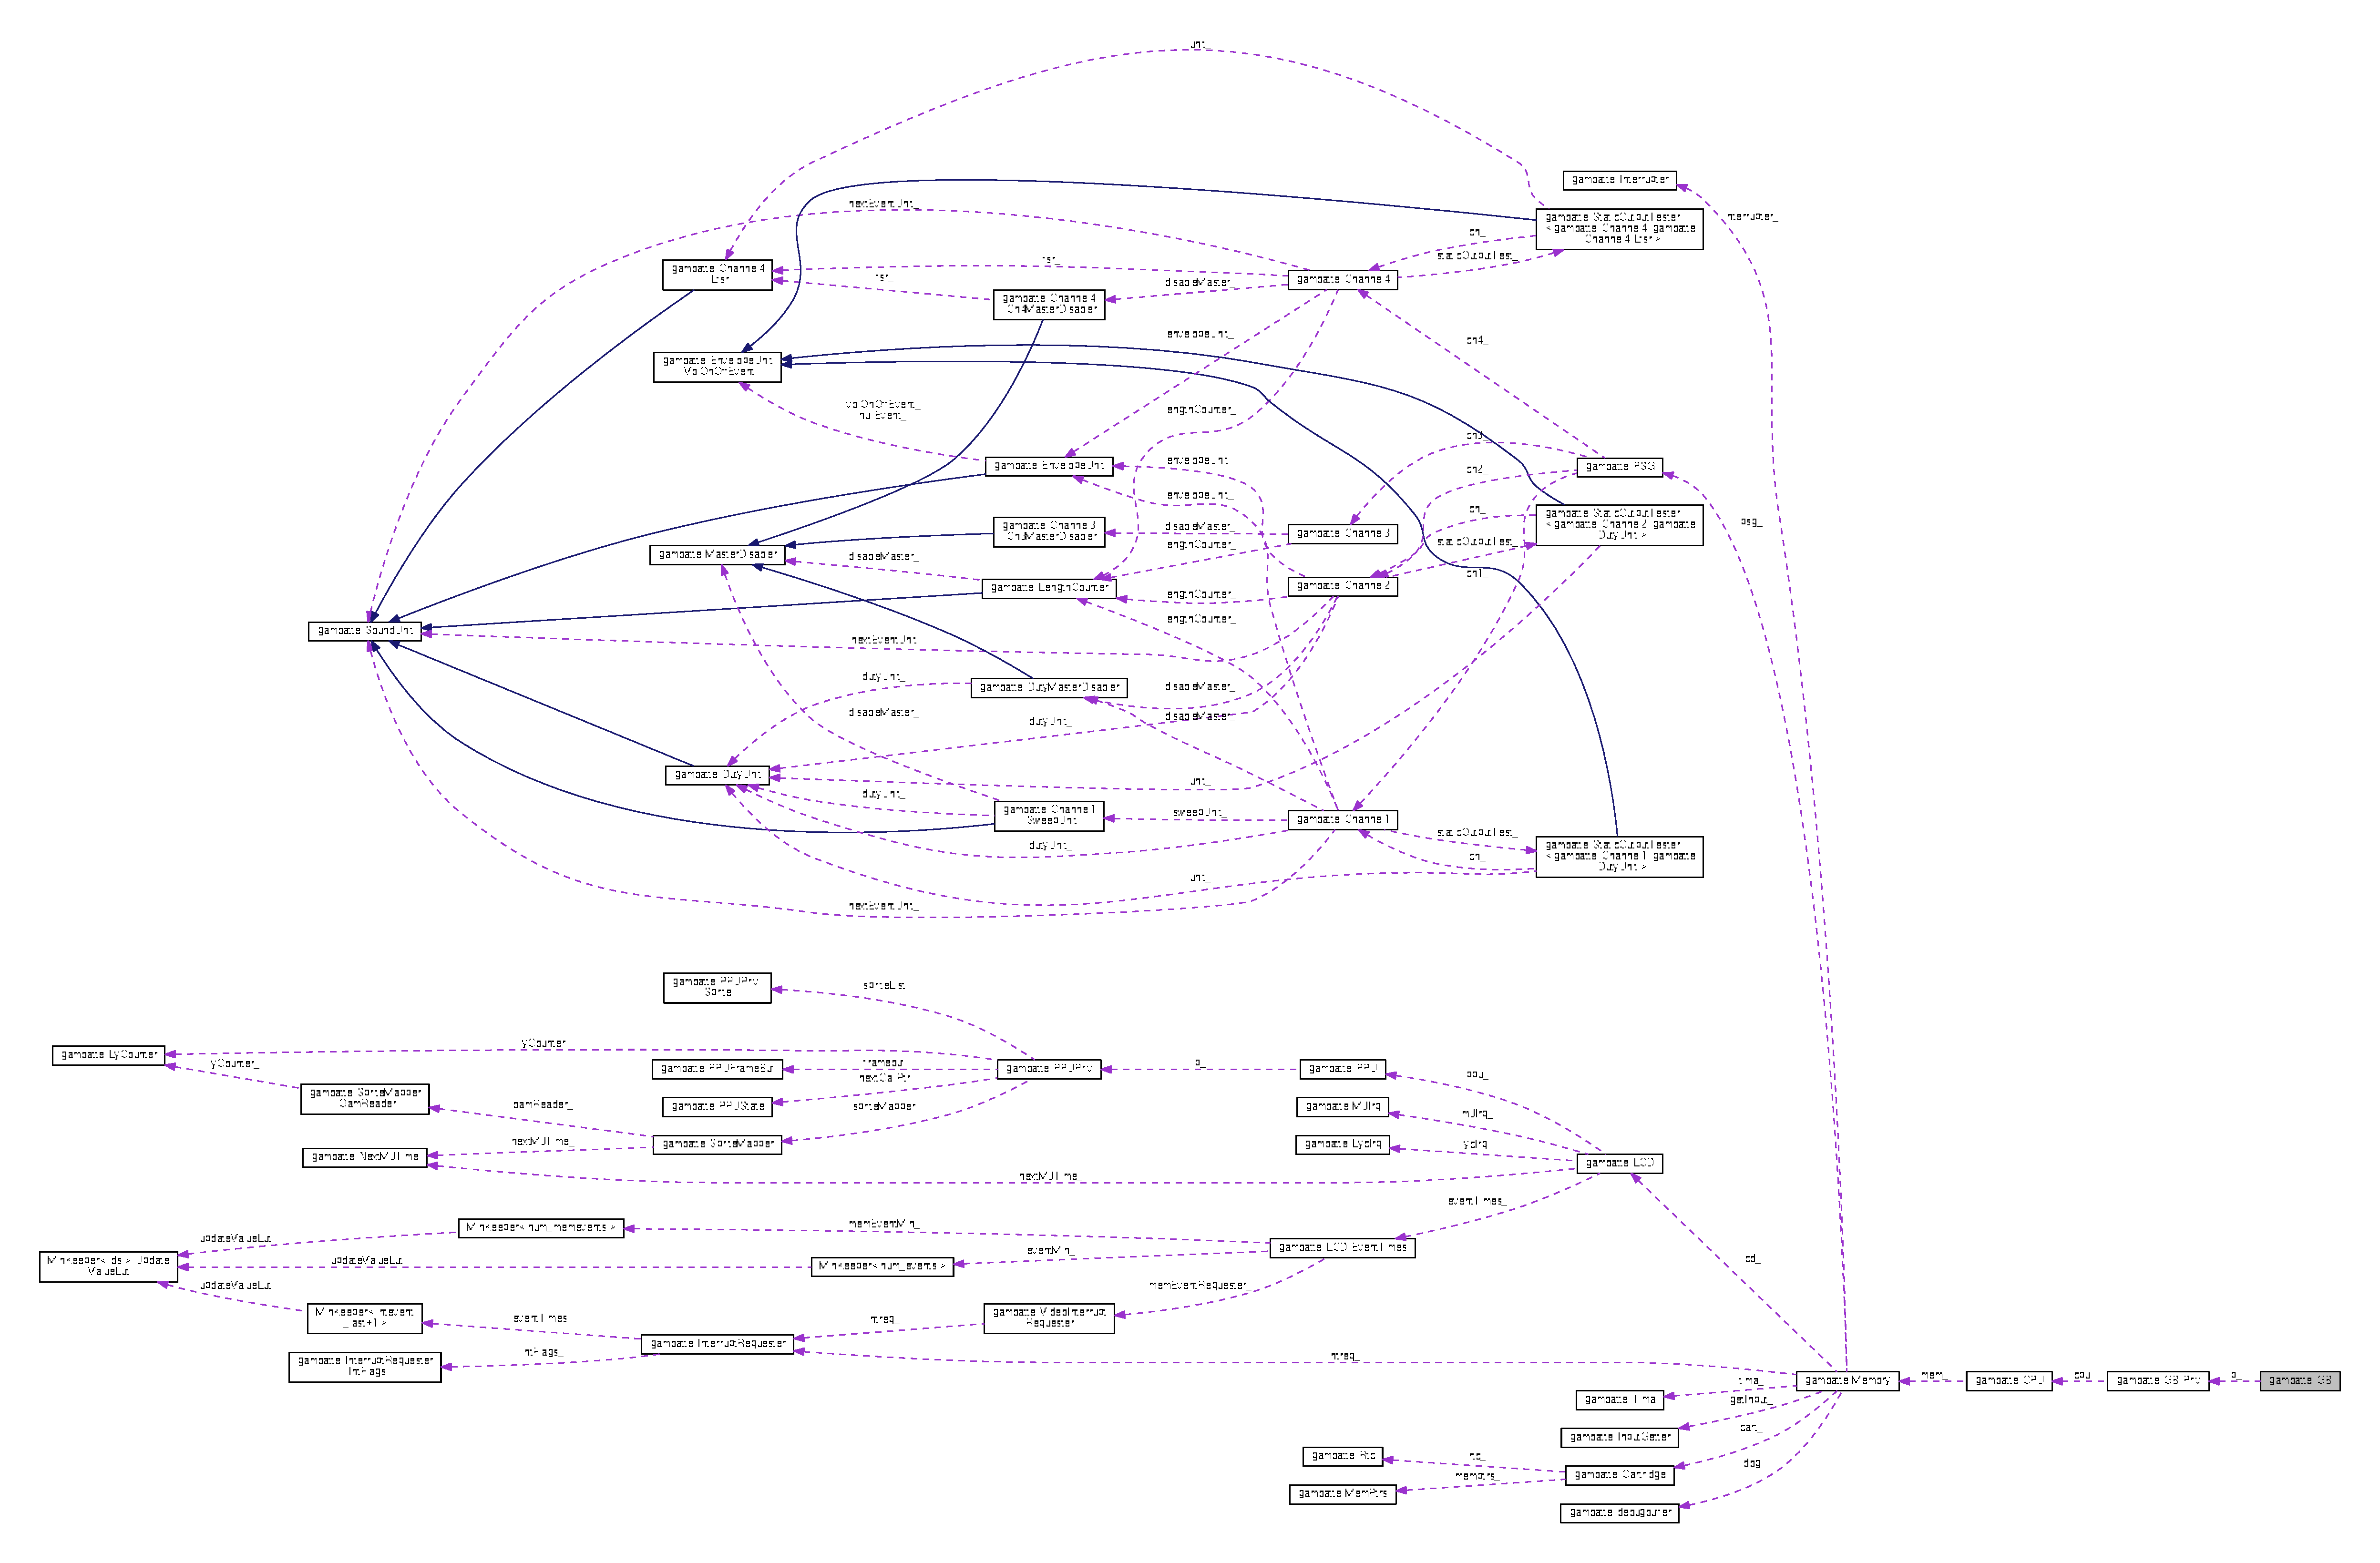
\includegraphics[width=350pt]{classgambatte_1_1GB__coll__graph}
\end{center}
\end{figure}
\subsection*{Classes}
\begin{DoxyCompactItemize}
\item 
struct \hyperlink{structgambatte_1_1GB_1_1Priv}{Priv}
\end{DoxyCompactItemize}
\subsection*{Public Types}
\begin{DoxyCompactItemize}
\item 
enum \hyperlink{classgambatte_1_1GB_a75a7553f8728e3d463c95dfdaaf48659}{Load\+Flag} \{ \hyperlink{classgambatte_1_1GB_a75a7553f8728e3d463c95dfdaaf48659ae801278f9c528c2ed3791d90b99f5e4f}{F\+O\+R\+C\+E\+\_\+\+D\+MG} = 1, 
\hyperlink{classgambatte_1_1GB_a75a7553f8728e3d463c95dfdaaf48659ad8d959b062a577c537fdf1700c1f89cd}{G\+B\+A\+\_\+\+C\+GB} = 2, 
\hyperlink{classgambatte_1_1GB_a75a7553f8728e3d463c95dfdaaf48659a5d01ba70d15c25f4d772b2096c6cdcbe}{M\+U\+L\+T\+I\+C\+A\+R\+T\+\_\+\+C\+O\+M\+P\+AT} = 4
 \}
\item 
enum \hyperlink{classgambatte_1_1GB_afbfe723d7a5e73582401f77c75d13893}{cpu\+\_\+register} \{ \newline
\hyperlink{classgambatte_1_1GB_afbfe723d7a5e73582401f77c75d13893a54ec6ce49af9fa8357d365214f4ca998}{R\+E\+G\+\_\+\+C\+Y\+C\+L\+E\+C\+O\+U\+N\+T\+ER}, 
\hyperlink{classgambatte_1_1GB_afbfe723d7a5e73582401f77c75d13893a5d919896cca72f6dbfccce103a68b305}{R\+E\+G\+\_\+\+PC}, 
\hyperlink{classgambatte_1_1GB_afbfe723d7a5e73582401f77c75d13893a52050914347a5d4fce3e8c785c4396ef}{R\+E\+G\+\_\+\+SP}, 
\hyperlink{classgambatte_1_1GB_afbfe723d7a5e73582401f77c75d13893a58a2991009182bfb8f99053a42320fd1}{R\+E\+G\+\_\+\+H\+F1}, 
\newline
\hyperlink{classgambatte_1_1GB_afbfe723d7a5e73582401f77c75d13893a73befef1e67e45ea94973869ab45f4b7}{R\+E\+G\+\_\+\+H\+F2}, 
\hyperlink{classgambatte_1_1GB_afbfe723d7a5e73582401f77c75d13893afa9db5119f7191e098ec7b2d85df49fb}{R\+E\+G\+\_\+\+ZF}, 
\hyperlink{classgambatte_1_1GB_afbfe723d7a5e73582401f77c75d13893a8a641defd8234773a9f0ab887e9ac6f6}{R\+E\+G\+\_\+\+CF}, 
\hyperlink{classgambatte_1_1GB_afbfe723d7a5e73582401f77c75d13893a51a78e8da5af0004ad7cd3dbf50042ec}{R\+E\+G\+\_\+A}, 
\newline
\hyperlink{classgambatte_1_1GB_afbfe723d7a5e73582401f77c75d13893abccee844a12cb88ddf5d10deee03a06d}{R\+E\+G\+\_\+B}, 
\hyperlink{classgambatte_1_1GB_afbfe723d7a5e73582401f77c75d13893a4a54977a065083fa30ab66d5c7ecb27d}{R\+E\+G\+\_\+C}, 
\hyperlink{classgambatte_1_1GB_afbfe723d7a5e73582401f77c75d13893a7bc1674813b4f515d707eb4c912d51f4}{R\+E\+G\+\_\+D}, 
\hyperlink{classgambatte_1_1GB_afbfe723d7a5e73582401f77c75d13893a5e13fb1dc281c2cfddbd7bab5f1e53cb}{R\+E\+G\+\_\+E}, 
\newline
\hyperlink{classgambatte_1_1GB_afbfe723d7a5e73582401f77c75d13893a49ca2a10c3abb9f3a68f165b2b419458}{R\+E\+G\+\_\+F}, 
\hyperlink{classgambatte_1_1GB_afbfe723d7a5e73582401f77c75d13893a7b4bb61a2f52b54f0fc18d9dc0ea89b8}{R\+E\+G\+\_\+H}, 
\hyperlink{classgambatte_1_1GB_afbfe723d7a5e73582401f77c75d13893a7333f03f48c8ad665a8de88a8fd58228}{R\+E\+G\+\_\+L}
 \}
\end{DoxyCompactItemize}
\subsection*{Public Member Functions}
\begin{DoxyCompactItemize}
\item 
\hyperlink{classgambatte_1_1GB_a360f22e656d5ff564eb0dea987ae71c7}{GB} ()
\item 
\hyperlink{classgambatte_1_1GB_a27727465be963f80f4fd96449a3d9c13}{$\sim$\+GB} ()
\item 
\hyperlink{namespacegambatte_a42606f494711d2e2870a5f5cdf69e468}{Load\+Res} \hyperlink{classgambatte_1_1GB_a3eb7cf83b1634dacc796971760b31fa2}{load} (std\+::string const \&romfile, unsigned flags=0)
\item 
\hyperlink{namespacegambatte_a42606f494711d2e2870a5f5cdf69e468}{Load\+Res} \hyperlink{classgambatte_1_1GB_a4ee8c151c978541fe20a282bdcc68969}{load} (const unsigned char $\ast$image, size\+\_\+t isize, unsigned flags=0)
\item 
signed \hyperlink{classgambatte_1_1GB_a10d409c2865b9c9770bf2a19f6d77dd7}{run\+For} (\hyperlink{namespacegambatte_a0639f09fccfbbd5a8e0796318768e370}{gambatte\+::uint\+\_\+least32\+\_\+t} $\ast$video\+Buf, std\+::ptrdiff\+\_\+t pitch, \hyperlink{namespacegambatte_a0639f09fccfbbd5a8e0796318768e370}{gambatte\+::uint\+\_\+least32\+\_\+t} $\ast$sound\+Buf, unsigned \&samples)
\item 
void \hyperlink{classgambatte_1_1GB_a765c0a392c9801ab094936f2978b5000}{reset} ()
\item 
void \hyperlink{classgambatte_1_1GB_a051afa03a39e9012d5c64ea0c6e3e852}{set\+Dmg\+Palette\+Color} (\hyperlink{ioapi_8h_a787fa3cf048117ba7123753c1e74fcd6}{int} pal\+Num, \hyperlink{ioapi_8h_a787fa3cf048117ba7123753c1e74fcd6}{int} color\+Num, \hyperlink{namespacegambatte_a0639f09fccfbbd5a8e0796318768e370}{uint\+\_\+least32\+\_\+t} rgb32)
\item 
void \hyperlink{classgambatte_1_1GB_a7b722194c9472371c28285cdbf35e70f}{set\+Input\+Getter} (\hyperlink{classgambatte_1_1InputGetter}{Input\+Getter} $\ast$get\+Input)
\item 
void \hyperlink{classgambatte_1_1GB_ae5d14de04bb821ccdc2bc4d4dbc649c2}{set\+Save\+Dir} (std\+::string const \&sdir)
\item 
bool \hyperlink{classgambatte_1_1GB_a96ffbde272ed65919f851740682cac04}{is\+Cgb} () const
\item 
bool \hyperlink{classgambatte_1_1GB_ae7b16fcdf62d8dcd3c17cc1c5cad223e}{is\+Loaded} () const
\item 
void \hyperlink{classgambatte_1_1GB_a465fec5e623d8ec44c4c00fed15ed387}{save\+Savedata} ()
\item 
bool \hyperlink{classgambatte_1_1GB_a4762c3580bafcdd7635988ee8b034869}{save\+State} (\hyperlink{namespacegambatte_a0639f09fccfbbd5a8e0796318768e370}{gambatte\+::uint\+\_\+least32\+\_\+t} const $\ast$video\+Buf, std\+::ptrdiff\+\_\+t pitch)
\item 
bool \hyperlink{classgambatte_1_1GB_a70781b0ddbfd7d52ae6bc0db1c34be0d}{load\+State} ()
\item 
bool \hyperlink{classgambatte_1_1GB_a98b621fc4632d6c815c6eeb31a59d972}{save\+State} (\hyperlink{namespacegambatte_a0639f09fccfbbd5a8e0796318768e370}{gambatte\+::uint\+\_\+least32\+\_\+t} const $\ast$video\+Buf, std\+::ptrdiff\+\_\+t pitch, std\+::string const \&filepath)
\item 
bool \hyperlink{classgambatte_1_1GB_a7ac605f7586d955acb408a649bc3faf1}{load\+State} (std\+::string const \&filepath)
\item 
void \hyperlink{classgambatte_1_1GB_af6c45af52b0ec127ddcb00a2d32d6b18}{save\+State} (std\+::vector$<$ char $>$ \&data, const std\+::vector$<$ char $>$ \&cmpdata)
\item 
void \hyperlink{classgambatte_1_1GB_a26dfbfcb3487893188f74bd419c8f23e}{save\+State} (std\+::vector$<$ char $>$ \&data)
\item 
void \hyperlink{classgambatte_1_1GB_a8745c11c1ab010ac43147d537c35fb79}{load\+State} (const std\+::vector$<$ char $>$ \&data)
\item 
void \hyperlink{classgambatte_1_1GB_a231371a6ef7aa0001afa45d645052569}{select\+State} (\hyperlink{ioapi_8h_a787fa3cf048117ba7123753c1e74fcd6}{int} n)
\item 
\hyperlink{ioapi_8h_a787fa3cf048117ba7123753c1e74fcd6}{int} \hyperlink{classgambatte_1_1GB_a48d11dcf693f45ab861f640d8fa96dc9}{current\+State} () const
\item 
std\+::string const \hyperlink{classgambatte_1_1GB_ad3eeb7e32908992b471c44936f05f8ea}{rom\+Title} () const
\item 
class \hyperlink{classgambatte_1_1PakInfo}{Pak\+Info} const \hyperlink{classgambatte_1_1GB_a53f8602582e710cb1938ff6d1306bde9}{pak\+Info} () const
\item 
void \hyperlink{classgambatte_1_1GB_ab39e81dad0d44900154c8c555b39d35c}{set\+Game\+Genie} (std\+::string const \&codes)
\item 
void \hyperlink{classgambatte_1_1GB_a056a4e6a182ef54c54afff0516b3721c}{set\+Game\+Shark} (std\+::string const \&codes)
\item 
void \hyperlink{classgambatte_1_1GB_a6beebe28f631880573d8e6a91ceb675f}{set\+Rtc\+Base} (time\+\_\+t time)
\item 
time\+\_\+t \hyperlink{classgambatte_1_1GB_a8fd5bd2699640686ad21e211ca841c2f}{get\+Rtc\+Base} ()
\item 
std\+::pair$<$ unsigned char $\ast$, size\+\_\+t $>$ \hyperlink{classgambatte_1_1GB_a0781cb0969c57ddc0fa647b54ee373f6}{get\+Work\+Ram} ()
\item 
std\+::pair$<$ unsigned char $\ast$, size\+\_\+t $>$ \hyperlink{classgambatte_1_1GB_aef4cbcec5818d26bef8c54cedf007e17}{get\+Save\+Ram} ()
\item 
std\+::pair$<$ unsigned char $\ast$, size\+\_\+t $>$ \hyperlink{classgambatte_1_1GB_af97601bcf082aafab539a6922f36beb8}{get\+Io\+Ram} ()
\item 
std\+::pair$<$ unsigned char $\ast$, size\+\_\+t $>$ \hyperlink{classgambatte_1_1GB_af72f3d0e4a022d737bff406d3327038b}{get\+Video\+Ram} ()
\item 
void \hyperlink{classgambatte_1_1GB_a910300b95fe3c38e7d6c0b3f11c017c5}{set\+\_\+walltime\+\_\+fn} (time\+\_\+t($\ast$\+\_\+walltime)())
\item 
uint32\+\_\+t \hyperlink{classgambatte_1_1GB_a5d93be3dc403febfd05f65987fffbd96}{get\+\_\+cpureg} (enum \hyperlink{classgambatte_1_1GB_afbfe723d7a5e73582401f77c75d13893}{cpu\+\_\+register} reg)
\item 
void \hyperlink{classgambatte_1_1GB_a4c4ac99f71f96e9c8a0ae7b5ad1a2245}{set\+\_\+cpureg} (enum \hyperlink{classgambatte_1_1GB_afbfe723d7a5e73582401f77c75d13893}{cpu\+\_\+register} reg, uint32\+\_\+t val)
\item 
void \hyperlink{classgambatte_1_1GB_a87d311a79eef1d8a812cbd8ba82f0715}{set\+\_\+debug\+\_\+buffer} (\hyperlink{structgambatte_1_1debugbuffer}{debugbuffer} \&dbgbuf)
\item 
uint8\+\_\+t \hyperlink{classgambatte_1_1GB_acafddce904037bfa513b7b27f0f4ffae}{bus\+\_\+read} (unsigned addr)
\item 
void \hyperlink{classgambatte_1_1GB_a060622967acdfc0ff693dedc39d9d187}{bus\+\_\+write} (unsigned addr, uint8\+\_\+t val)
\item 
void \hyperlink{classgambatte_1_1GB_a46e4849dcde049e8667cd282864389d5}{set\+\_\+emuflags} (unsigned flags)
\item 
void \hyperlink{classgambatte_1_1GB_a8efc0744b106fb4163e048b8c5f0ca61}{print\+\_\+interrupt\+\_\+timing} (void)
\end{DoxyCompactItemize}
\subsection*{Static Public Member Functions}
\begin{DoxyCompactItemize}
\item 
static std\+::string \hyperlink{classgambatte_1_1GB_a2b1912a87c68f5483ed2272cafdd5648}{version} ()
\end{DoxyCompactItemize}
\subsection*{Private Member Functions}
\begin{DoxyCompactItemize}
\item 
void \hyperlink{classgambatte_1_1GB_adb4e65eec2d20a2f31c6b66e621c7859}{preload\+\_\+common} ()
\item 
void \hyperlink{classgambatte_1_1GB_a9e9b8ed4d0d978cfa6c09c849e704fe7}{postload\+\_\+common} (const unsigned flags)
\item 
\hyperlink{classgambatte_1_1GB_a8f53e9b7823f40e90a0c84a5f088b712}{GB} (\hyperlink{classgambatte_1_1GB}{GB} const \&)
\item 
\hyperlink{classgambatte_1_1GB}{GB} \& \hyperlink{classgambatte_1_1GB_a621e7cd52ce6278c5a521d024b995df5}{operator=} (\hyperlink{classgambatte_1_1GB}{GB} const \&)
\end{DoxyCompactItemize}
\subsection*{Private Attributes}
\begin{DoxyCompactItemize}
\item 
\hyperlink{structgambatte_1_1GB_1_1Priv}{Priv} $\ast$const \hyperlink{classgambatte_1_1GB_a648f96b5ea58e1d6c8013c8897e63218}{p\+\_\+}
\item 
time\+\_\+t($\ast$ \hyperlink{classgambatte_1_1GB_a3b230d27feb2c167823bce8cfc6b02af}{walltime} )()
\end{DoxyCompactItemize}


\subsection{Member Enumeration Documentation}
\mbox{\Hypertarget{classgambatte_1_1GB_afbfe723d7a5e73582401f77c75d13893}\label{classgambatte_1_1GB_afbfe723d7a5e73582401f77c75d13893}} 
\index{gambatte\+::\+GB@{gambatte\+::\+GB}!cpu\+\_\+register@{cpu\+\_\+register}}
\index{cpu\+\_\+register@{cpu\+\_\+register}!gambatte\+::\+GB@{gambatte\+::\+GB}}
\subsubsection{\texorpdfstring{cpu\+\_\+register}{cpu\_register}}
{\footnotesize\ttfamily enum \hyperlink{classgambatte_1_1GB_afbfe723d7a5e73582401f77c75d13893}{gambatte\+::\+G\+B\+::cpu\+\_\+register}}

\hyperlink{classgambatte_1_1CPU}{C\+PU} registers. \begin{DoxyEnumFields}{Enumerator}
\raisebox{\heightof{T}}[0pt][0pt]{\index{R\+E\+G\+\_\+\+C\+Y\+C\+L\+E\+C\+O\+U\+N\+T\+ER@{R\+E\+G\+\_\+\+C\+Y\+C\+L\+E\+C\+O\+U\+N\+T\+ER}!gambatte\+::\+GB@{gambatte\+::\+GB}}\index{gambatte\+::\+GB@{gambatte\+::\+GB}!R\+E\+G\+\_\+\+C\+Y\+C\+L\+E\+C\+O\+U\+N\+T\+ER@{R\+E\+G\+\_\+\+C\+Y\+C\+L\+E\+C\+O\+U\+N\+T\+ER}}}\mbox{\Hypertarget{classgambatte_1_1GB_afbfe723d7a5e73582401f77c75d13893a54ec6ce49af9fa8357d365214f4ca998}\label{classgambatte_1_1GB_afbfe723d7a5e73582401f77c75d13893a54ec6ce49af9fa8357d365214f4ca998}} 
R\+E\+G\+\_\+\+C\+Y\+C\+L\+E\+C\+O\+U\+N\+T\+ER&\\
\hline

\raisebox{\heightof{T}}[0pt][0pt]{\index{R\+E\+G\+\_\+\+PC@{R\+E\+G\+\_\+\+PC}!gambatte\+::\+GB@{gambatte\+::\+GB}}\index{gambatte\+::\+GB@{gambatte\+::\+GB}!R\+E\+G\+\_\+\+PC@{R\+E\+G\+\_\+\+PC}}}\mbox{\Hypertarget{classgambatte_1_1GB_afbfe723d7a5e73582401f77c75d13893a5d919896cca72f6dbfccce103a68b305}\label{classgambatte_1_1GB_afbfe723d7a5e73582401f77c75d13893a5d919896cca72f6dbfccce103a68b305}} 
R\+E\+G\+\_\+\+PC&\\
\hline

\raisebox{\heightof{T}}[0pt][0pt]{\index{R\+E\+G\+\_\+\+SP@{R\+E\+G\+\_\+\+SP}!gambatte\+::\+GB@{gambatte\+::\+GB}}\index{gambatte\+::\+GB@{gambatte\+::\+GB}!R\+E\+G\+\_\+\+SP@{R\+E\+G\+\_\+\+SP}}}\mbox{\Hypertarget{classgambatte_1_1GB_afbfe723d7a5e73582401f77c75d13893a52050914347a5d4fce3e8c785c4396ef}\label{classgambatte_1_1GB_afbfe723d7a5e73582401f77c75d13893a52050914347a5d4fce3e8c785c4396ef}} 
R\+E\+G\+\_\+\+SP&\\
\hline

\raisebox{\heightof{T}}[0pt][0pt]{\index{R\+E\+G\+\_\+\+H\+F1@{R\+E\+G\+\_\+\+H\+F1}!gambatte\+::\+GB@{gambatte\+::\+GB}}\index{gambatte\+::\+GB@{gambatte\+::\+GB}!R\+E\+G\+\_\+\+H\+F1@{R\+E\+G\+\_\+\+H\+F1}}}\mbox{\Hypertarget{classgambatte_1_1GB_afbfe723d7a5e73582401f77c75d13893a58a2991009182bfb8f99053a42320fd1}\label{classgambatte_1_1GB_afbfe723d7a5e73582401f77c75d13893a58a2991009182bfb8f99053a42320fd1}} 
R\+E\+G\+\_\+\+H\+F1&\\
\hline

\raisebox{\heightof{T}}[0pt][0pt]{\index{R\+E\+G\+\_\+\+H\+F2@{R\+E\+G\+\_\+\+H\+F2}!gambatte\+::\+GB@{gambatte\+::\+GB}}\index{gambatte\+::\+GB@{gambatte\+::\+GB}!R\+E\+G\+\_\+\+H\+F2@{R\+E\+G\+\_\+\+H\+F2}}}\mbox{\Hypertarget{classgambatte_1_1GB_afbfe723d7a5e73582401f77c75d13893a73befef1e67e45ea94973869ab45f4b7}\label{classgambatte_1_1GB_afbfe723d7a5e73582401f77c75d13893a73befef1e67e45ea94973869ab45f4b7}} 
R\+E\+G\+\_\+\+H\+F2&\\
\hline

\raisebox{\heightof{T}}[0pt][0pt]{\index{R\+E\+G\+\_\+\+ZF@{R\+E\+G\+\_\+\+ZF}!gambatte\+::\+GB@{gambatte\+::\+GB}}\index{gambatte\+::\+GB@{gambatte\+::\+GB}!R\+E\+G\+\_\+\+ZF@{R\+E\+G\+\_\+\+ZF}}}\mbox{\Hypertarget{classgambatte_1_1GB_afbfe723d7a5e73582401f77c75d13893afa9db5119f7191e098ec7b2d85df49fb}\label{classgambatte_1_1GB_afbfe723d7a5e73582401f77c75d13893afa9db5119f7191e098ec7b2d85df49fb}} 
R\+E\+G\+\_\+\+ZF&\\
\hline

\raisebox{\heightof{T}}[0pt][0pt]{\index{R\+E\+G\+\_\+\+CF@{R\+E\+G\+\_\+\+CF}!gambatte\+::\+GB@{gambatte\+::\+GB}}\index{gambatte\+::\+GB@{gambatte\+::\+GB}!R\+E\+G\+\_\+\+CF@{R\+E\+G\+\_\+\+CF}}}\mbox{\Hypertarget{classgambatte_1_1GB_afbfe723d7a5e73582401f77c75d13893a8a641defd8234773a9f0ab887e9ac6f6}\label{classgambatte_1_1GB_afbfe723d7a5e73582401f77c75d13893a8a641defd8234773a9f0ab887e9ac6f6}} 
R\+E\+G\+\_\+\+CF&\\
\hline

\raisebox{\heightof{T}}[0pt][0pt]{\index{R\+E\+G\+\_\+A@{R\+E\+G\+\_\+A}!gambatte\+::\+GB@{gambatte\+::\+GB}}\index{gambatte\+::\+GB@{gambatte\+::\+GB}!R\+E\+G\+\_\+A@{R\+E\+G\+\_\+A}}}\mbox{\Hypertarget{classgambatte_1_1GB_afbfe723d7a5e73582401f77c75d13893a51a78e8da5af0004ad7cd3dbf50042ec}\label{classgambatte_1_1GB_afbfe723d7a5e73582401f77c75d13893a51a78e8da5af0004ad7cd3dbf50042ec}} 
R\+E\+G\+\_\+A&\\
\hline

\raisebox{\heightof{T}}[0pt][0pt]{\index{R\+E\+G\+\_\+B@{R\+E\+G\+\_\+B}!gambatte\+::\+GB@{gambatte\+::\+GB}}\index{gambatte\+::\+GB@{gambatte\+::\+GB}!R\+E\+G\+\_\+B@{R\+E\+G\+\_\+B}}}\mbox{\Hypertarget{classgambatte_1_1GB_afbfe723d7a5e73582401f77c75d13893abccee844a12cb88ddf5d10deee03a06d}\label{classgambatte_1_1GB_afbfe723d7a5e73582401f77c75d13893abccee844a12cb88ddf5d10deee03a06d}} 
R\+E\+G\+\_\+B&\\
\hline

\raisebox{\heightof{T}}[0pt][0pt]{\index{R\+E\+G\+\_\+C@{R\+E\+G\+\_\+C}!gambatte\+::\+GB@{gambatte\+::\+GB}}\index{gambatte\+::\+GB@{gambatte\+::\+GB}!R\+E\+G\+\_\+C@{R\+E\+G\+\_\+C}}}\mbox{\Hypertarget{classgambatte_1_1GB_afbfe723d7a5e73582401f77c75d13893a4a54977a065083fa30ab66d5c7ecb27d}\label{classgambatte_1_1GB_afbfe723d7a5e73582401f77c75d13893a4a54977a065083fa30ab66d5c7ecb27d}} 
R\+E\+G\+\_\+C&\\
\hline

\raisebox{\heightof{T}}[0pt][0pt]{\index{R\+E\+G\+\_\+D@{R\+E\+G\+\_\+D}!gambatte\+::\+GB@{gambatte\+::\+GB}}\index{gambatte\+::\+GB@{gambatte\+::\+GB}!R\+E\+G\+\_\+D@{R\+E\+G\+\_\+D}}}\mbox{\Hypertarget{classgambatte_1_1GB_afbfe723d7a5e73582401f77c75d13893a7bc1674813b4f515d707eb4c912d51f4}\label{classgambatte_1_1GB_afbfe723d7a5e73582401f77c75d13893a7bc1674813b4f515d707eb4c912d51f4}} 
R\+E\+G\+\_\+D&\\
\hline

\raisebox{\heightof{T}}[0pt][0pt]{\index{R\+E\+G\+\_\+E@{R\+E\+G\+\_\+E}!gambatte\+::\+GB@{gambatte\+::\+GB}}\index{gambatte\+::\+GB@{gambatte\+::\+GB}!R\+E\+G\+\_\+E@{R\+E\+G\+\_\+E}}}\mbox{\Hypertarget{classgambatte_1_1GB_afbfe723d7a5e73582401f77c75d13893a5e13fb1dc281c2cfddbd7bab5f1e53cb}\label{classgambatte_1_1GB_afbfe723d7a5e73582401f77c75d13893a5e13fb1dc281c2cfddbd7bab5f1e53cb}} 
R\+E\+G\+\_\+E&\\
\hline

\raisebox{\heightof{T}}[0pt][0pt]{\index{R\+E\+G\+\_\+F@{R\+E\+G\+\_\+F}!gambatte\+::\+GB@{gambatte\+::\+GB}}\index{gambatte\+::\+GB@{gambatte\+::\+GB}!R\+E\+G\+\_\+F@{R\+E\+G\+\_\+F}}}\mbox{\Hypertarget{classgambatte_1_1GB_afbfe723d7a5e73582401f77c75d13893a49ca2a10c3abb9f3a68f165b2b419458}\label{classgambatte_1_1GB_afbfe723d7a5e73582401f77c75d13893a49ca2a10c3abb9f3a68f165b2b419458}} 
R\+E\+G\+\_\+F&\\
\hline

\raisebox{\heightof{T}}[0pt][0pt]{\index{R\+E\+G\+\_\+H@{R\+E\+G\+\_\+H}!gambatte\+::\+GB@{gambatte\+::\+GB}}\index{gambatte\+::\+GB@{gambatte\+::\+GB}!R\+E\+G\+\_\+H@{R\+E\+G\+\_\+H}}}\mbox{\Hypertarget{classgambatte_1_1GB_afbfe723d7a5e73582401f77c75d13893a7b4bb61a2f52b54f0fc18d9dc0ea89b8}\label{classgambatte_1_1GB_afbfe723d7a5e73582401f77c75d13893a7b4bb61a2f52b54f0fc18d9dc0ea89b8}} 
R\+E\+G\+\_\+H&\\
\hline

\raisebox{\heightof{T}}[0pt][0pt]{\index{R\+E\+G\+\_\+L@{R\+E\+G\+\_\+L}!gambatte\+::\+GB@{gambatte\+::\+GB}}\index{gambatte\+::\+GB@{gambatte\+::\+GB}!R\+E\+G\+\_\+L@{R\+E\+G\+\_\+L}}}\mbox{\Hypertarget{classgambatte_1_1GB_afbfe723d7a5e73582401f77c75d13893a7333f03f48c8ad665a8de88a8fd58228}\label{classgambatte_1_1GB_afbfe723d7a5e73582401f77c75d13893a7333f03f48c8ad665a8de88a8fd58228}} 
R\+E\+G\+\_\+L&\\
\hline

\end{DoxyEnumFields}
\mbox{\Hypertarget{classgambatte_1_1GB_a75a7553f8728e3d463c95dfdaaf48659}\label{classgambatte_1_1GB_a75a7553f8728e3d463c95dfdaaf48659}} 
\index{gambatte\+::\+GB@{gambatte\+::\+GB}!Load\+Flag@{Load\+Flag}}
\index{Load\+Flag@{Load\+Flag}!gambatte\+::\+GB@{gambatte\+::\+GB}}
\subsubsection{\texorpdfstring{Load\+Flag}{LoadFlag}}
{\footnotesize\ttfamily enum \hyperlink{classgambatte_1_1GB_a75a7553f8728e3d463c95dfdaaf48659}{gambatte\+::\+G\+B\+::\+Load\+Flag}}

\begin{DoxyEnumFields}{Enumerator}
\raisebox{\heightof{T}}[0pt][0pt]{\index{F\+O\+R\+C\+E\+\_\+\+D\+MG@{F\+O\+R\+C\+E\+\_\+\+D\+MG}!gambatte\+::\+GB@{gambatte\+::\+GB}}\index{gambatte\+::\+GB@{gambatte\+::\+GB}!F\+O\+R\+C\+E\+\_\+\+D\+MG@{F\+O\+R\+C\+E\+\_\+\+D\+MG}}}\mbox{\Hypertarget{classgambatte_1_1GB_a75a7553f8728e3d463c95dfdaaf48659ae801278f9c528c2ed3791d90b99f5e4f}\label{classgambatte_1_1GB_a75a7553f8728e3d463c95dfdaaf48659ae801278f9c528c2ed3791d90b99f5e4f}} 
F\+O\+R\+C\+E\+\_\+\+D\+MG&Treat the R\+OM as not having C\+GB support regardless of what its header advertises. \\
\hline

\raisebox{\heightof{T}}[0pt][0pt]{\index{G\+B\+A\+\_\+\+C\+GB@{G\+B\+A\+\_\+\+C\+GB}!gambatte\+::\+GB@{gambatte\+::\+GB}}\index{gambatte\+::\+GB@{gambatte\+::\+GB}!G\+B\+A\+\_\+\+C\+GB@{G\+B\+A\+\_\+\+C\+GB}}}\mbox{\Hypertarget{classgambatte_1_1GB_a75a7553f8728e3d463c95dfdaaf48659ad8d959b062a577c537fdf1700c1f89cd}\label{classgambatte_1_1GB_a75a7553f8728e3d463c95dfdaaf48659ad8d959b062a577c537fdf1700c1f89cd}} 
G\+B\+A\+\_\+\+C\+GB&Use G\+BA intial \hyperlink{classgambatte_1_1CPU}{C\+PU} register values when in C\+GB mode. \\
\hline

\raisebox{\heightof{T}}[0pt][0pt]{\index{M\+U\+L\+T\+I\+C\+A\+R\+T\+\_\+\+C\+O\+M\+P\+AT@{M\+U\+L\+T\+I\+C\+A\+R\+T\+\_\+\+C\+O\+M\+P\+AT}!gambatte\+::\+GB@{gambatte\+::\+GB}}\index{gambatte\+::\+GB@{gambatte\+::\+GB}!M\+U\+L\+T\+I\+C\+A\+R\+T\+\_\+\+C\+O\+M\+P\+AT@{M\+U\+L\+T\+I\+C\+A\+R\+T\+\_\+\+C\+O\+M\+P\+AT}}}\mbox{\Hypertarget{classgambatte_1_1GB_a75a7553f8728e3d463c95dfdaaf48659a5d01ba70d15c25f4d772b2096c6cdcbe}\label{classgambatte_1_1GB_a75a7553f8728e3d463c95dfdaaf48659a5d01ba70d15c25f4d772b2096c6cdcbe}} 
M\+U\+L\+T\+I\+C\+A\+R\+T\+\_\+\+C\+O\+M\+P\+AT&Use heuristics to detect and support some multicart M\+B\+Cs disguised as M\+B\+C1. \\
\hline

\end{DoxyEnumFields}


\subsection{Constructor \& Destructor Documentation}
\mbox{\Hypertarget{classgambatte_1_1GB_a360f22e656d5ff564eb0dea987ae71c7}\label{classgambatte_1_1GB_a360f22e656d5ff564eb0dea987ae71c7}} 
\index{gambatte\+::\+GB@{gambatte\+::\+GB}!GB@{GB}}
\index{GB@{GB}!gambatte\+::\+GB@{gambatte\+::\+GB}}
\subsubsection{\texorpdfstring{G\+B()}{GB()}\hspace{0.1cm}{\footnotesize\ttfamily [1/2]}}
{\footnotesize\ttfamily gambatte\+::\+G\+B\+::\+GB (\begin{DoxyParamCaption}{ }\end{DoxyParamCaption})}

\mbox{\Hypertarget{classgambatte_1_1GB_a27727465be963f80f4fd96449a3d9c13}\label{classgambatte_1_1GB_a27727465be963f80f4fd96449a3d9c13}} 
\index{gambatte\+::\+GB@{gambatte\+::\+GB}!````~GB@{$\sim$\+GB}}
\index{````~GB@{$\sim$\+GB}!gambatte\+::\+GB@{gambatte\+::\+GB}}
\subsubsection{\texorpdfstring{$\sim$\+G\+B()}{~GB()}}
{\footnotesize\ttfamily gambatte\+::\+G\+B\+::$\sim$\+GB (\begin{DoxyParamCaption}{ }\end{DoxyParamCaption})}

\mbox{\Hypertarget{classgambatte_1_1GB_a8f53e9b7823f40e90a0c84a5f088b712}\label{classgambatte_1_1GB_a8f53e9b7823f40e90a0c84a5f088b712}} 
\index{gambatte\+::\+GB@{gambatte\+::\+GB}!GB@{GB}}
\index{GB@{GB}!gambatte\+::\+GB@{gambatte\+::\+GB}}
\subsubsection{\texorpdfstring{G\+B()}{GB()}\hspace{0.1cm}{\footnotesize\ttfamily [2/2]}}
{\footnotesize\ttfamily gambatte\+::\+G\+B\+::\+GB (\begin{DoxyParamCaption}\item[{\hyperlink{classgambatte_1_1GB}{GB} const \&}]{ }\end{DoxyParamCaption})\hspace{0.3cm}{\ttfamily [private]}}



\subsection{Member Function Documentation}
\mbox{\Hypertarget{classgambatte_1_1GB_acafddce904037bfa513b7b27f0f4ffae}\label{classgambatte_1_1GB_acafddce904037bfa513b7b27f0f4ffae}} 
\index{gambatte\+::\+GB@{gambatte\+::\+GB}!bus\+\_\+read@{bus\+\_\+read}}
\index{bus\+\_\+read@{bus\+\_\+read}!gambatte\+::\+GB@{gambatte\+::\+GB}}
\subsubsection{\texorpdfstring{bus\+\_\+read()}{bus\_read()}}
{\footnotesize\ttfamily uint8\+\_\+t gambatte\+::\+G\+B\+::bus\+\_\+read (\begin{DoxyParamCaption}\item[{unsigned}]{addr }\end{DoxyParamCaption})}

\mbox{\Hypertarget{classgambatte_1_1GB_a060622967acdfc0ff693dedc39d9d187}\label{classgambatte_1_1GB_a060622967acdfc0ff693dedc39d9d187}} 
\index{gambatte\+::\+GB@{gambatte\+::\+GB}!bus\+\_\+write@{bus\+\_\+write}}
\index{bus\+\_\+write@{bus\+\_\+write}!gambatte\+::\+GB@{gambatte\+::\+GB}}
\subsubsection{\texorpdfstring{bus\+\_\+write()}{bus\_write()}}
{\footnotesize\ttfamily void gambatte\+::\+G\+B\+::bus\+\_\+write (\begin{DoxyParamCaption}\item[{unsigned}]{addr,  }\item[{uint8\+\_\+t}]{val }\end{DoxyParamCaption})}

\mbox{\Hypertarget{classgambatte_1_1GB_a48d11dcf693f45ab861f640d8fa96dc9}\label{classgambatte_1_1GB_a48d11dcf693f45ab861f640d8fa96dc9}} 
\index{gambatte\+::\+GB@{gambatte\+::\+GB}!current\+State@{current\+State}}
\index{current\+State@{current\+State}!gambatte\+::\+GB@{gambatte\+::\+GB}}
\subsubsection{\texorpdfstring{current\+State()}{currentState()}}
{\footnotesize\ttfamily \hyperlink{ioapi_8h_a787fa3cf048117ba7123753c1e74fcd6}{int} gambatte\+::\+G\+B\+::current\+State (\begin{DoxyParamCaption}{ }\end{DoxyParamCaption}) const}

Current state slot selected with \hyperlink{classgambatte_1_1GB_a231371a6ef7aa0001afa45d645052569}{select\+State()}. Returns a value between 0 and 9 inclusive. \mbox{\Hypertarget{classgambatte_1_1GB_a5d93be3dc403febfd05f65987fffbd96}\label{classgambatte_1_1GB_a5d93be3dc403febfd05f65987fffbd96}} 
\index{gambatte\+::\+GB@{gambatte\+::\+GB}!get\+\_\+cpureg@{get\+\_\+cpureg}}
\index{get\+\_\+cpureg@{get\+\_\+cpureg}!gambatte\+::\+GB@{gambatte\+::\+GB}}
\subsubsection{\texorpdfstring{get\+\_\+cpureg()}{get\_cpureg()}}
{\footnotesize\ttfamily uint32\+\_\+t gambatte\+::\+G\+B\+::get\+\_\+cpureg (\begin{DoxyParamCaption}\item[{enum \hyperlink{classgambatte_1_1GB_afbfe723d7a5e73582401f77c75d13893}{cpu\+\_\+register}}]{reg }\end{DoxyParamCaption})}

\mbox{\Hypertarget{classgambatte_1_1GB_af97601bcf082aafab539a6922f36beb8}\label{classgambatte_1_1GB_af97601bcf082aafab539a6922f36beb8}} 
\index{gambatte\+::\+GB@{gambatte\+::\+GB}!get\+Io\+Ram@{get\+Io\+Ram}}
\index{get\+Io\+Ram@{get\+Io\+Ram}!gambatte\+::\+GB@{gambatte\+::\+GB}}
\subsubsection{\texorpdfstring{get\+Io\+Ram()}{getIoRam()}}
{\footnotesize\ttfamily std\+::pair$<$ unsigned char $\ast$, size\+\_\+t $>$ gambatte\+::\+G\+B\+::get\+Io\+Ram (\begin{DoxyParamCaption}{ }\end{DoxyParamCaption})}

Get pointer and size to I/O R\+AM. \begin{DoxyReturn}{Returns}
The pointer and size of I/O R\+AM. 
\end{DoxyReturn}
\mbox{\Hypertarget{classgambatte_1_1GB_a8fd5bd2699640686ad21e211ca841c2f}\label{classgambatte_1_1GB_a8fd5bd2699640686ad21e211ca841c2f}} 
\index{gambatte\+::\+GB@{gambatte\+::\+GB}!get\+Rtc\+Base@{get\+Rtc\+Base}}
\index{get\+Rtc\+Base@{get\+Rtc\+Base}!gambatte\+::\+GB@{gambatte\+::\+GB}}
\subsubsection{\texorpdfstring{get\+Rtc\+Base()}{getRtcBase()}}
{\footnotesize\ttfamily time\+\_\+t gambatte\+::\+G\+B\+::get\+Rtc\+Base (\begin{DoxyParamCaption}{ }\end{DoxyParamCaption})}

Get R\+TC base time. \mbox{\Hypertarget{classgambatte_1_1GB_aef4cbcec5818d26bef8c54cedf007e17}\label{classgambatte_1_1GB_aef4cbcec5818d26bef8c54cedf007e17}} 
\index{gambatte\+::\+GB@{gambatte\+::\+GB}!get\+Save\+Ram@{get\+Save\+Ram}}
\index{get\+Save\+Ram@{get\+Save\+Ram}!gambatte\+::\+GB@{gambatte\+::\+GB}}
\subsubsection{\texorpdfstring{get\+Save\+Ram()}{getSaveRam()}}
{\footnotesize\ttfamily std\+::pair$<$ unsigned char $\ast$, size\+\_\+t $>$ gambatte\+::\+G\+B\+::get\+Save\+Ram (\begin{DoxyParamCaption}{ }\end{DoxyParamCaption})}

Get pointer and size to Save R\+AM. \begin{DoxyReturn}{Returns}
The pointer and size of Save R\+AM. 
\end{DoxyReturn}
\mbox{\Hypertarget{classgambatte_1_1GB_af72f3d0e4a022d737bff406d3327038b}\label{classgambatte_1_1GB_af72f3d0e4a022d737bff406d3327038b}} 
\index{gambatte\+::\+GB@{gambatte\+::\+GB}!get\+Video\+Ram@{get\+Video\+Ram}}
\index{get\+Video\+Ram@{get\+Video\+Ram}!gambatte\+::\+GB@{gambatte\+::\+GB}}
\subsubsection{\texorpdfstring{get\+Video\+Ram()}{getVideoRam()}}
{\footnotesize\ttfamily std\+::pair$<$ unsigned char $\ast$, size\+\_\+t $>$ gambatte\+::\+G\+B\+::get\+Video\+Ram (\begin{DoxyParamCaption}{ }\end{DoxyParamCaption})}

Get pointer and size to Video R\+AM. \begin{DoxyReturn}{Returns}
The pointer and size of Video R\+AM. 
\end{DoxyReturn}
\mbox{\Hypertarget{classgambatte_1_1GB_a0781cb0969c57ddc0fa647b54ee373f6}\label{classgambatte_1_1GB_a0781cb0969c57ddc0fa647b54ee373f6}} 
\index{gambatte\+::\+GB@{gambatte\+::\+GB}!get\+Work\+Ram@{get\+Work\+Ram}}
\index{get\+Work\+Ram@{get\+Work\+Ram}!gambatte\+::\+GB@{gambatte\+::\+GB}}
\subsubsection{\texorpdfstring{get\+Work\+Ram()}{getWorkRam()}}
{\footnotesize\ttfamily std\+::pair$<$ unsigned char $\ast$, size\+\_\+t $>$ gambatte\+::\+G\+B\+::get\+Work\+Ram (\begin{DoxyParamCaption}{ }\end{DoxyParamCaption})}

Get pointer and size to Work R\+AM. \begin{DoxyReturn}{Returns}
The pointer and size of Work R\+AM. 
\end{DoxyReturn}
\mbox{\Hypertarget{classgambatte_1_1GB_a96ffbde272ed65919f851740682cac04}\label{classgambatte_1_1GB_a96ffbde272ed65919f851740682cac04}} 
\index{gambatte\+::\+GB@{gambatte\+::\+GB}!is\+Cgb@{is\+Cgb}}
\index{is\+Cgb@{is\+Cgb}!gambatte\+::\+GB@{gambatte\+::\+GB}}
\subsubsection{\texorpdfstring{is\+Cgb()}{isCgb()}}
{\footnotesize\ttfamily bool gambatte\+::\+G\+B\+::is\+Cgb (\begin{DoxyParamCaption}{ }\end{DoxyParamCaption}) const}

Returns true if the currently loaded R\+OM image is treated as having C\+GB support. \mbox{\Hypertarget{classgambatte_1_1GB_ae7b16fcdf62d8dcd3c17cc1c5cad223e}\label{classgambatte_1_1GB_ae7b16fcdf62d8dcd3c17cc1c5cad223e}} 
\index{gambatte\+::\+GB@{gambatte\+::\+GB}!is\+Loaded@{is\+Loaded}}
\index{is\+Loaded@{is\+Loaded}!gambatte\+::\+GB@{gambatte\+::\+GB}}
\subsubsection{\texorpdfstring{is\+Loaded()}{isLoaded()}}
{\footnotesize\ttfamily bool gambatte\+::\+G\+B\+::is\+Loaded (\begin{DoxyParamCaption}{ }\end{DoxyParamCaption}) const}

Returns true if a R\+OM image is loaded. \mbox{\Hypertarget{classgambatte_1_1GB_a3eb7cf83b1634dacc796971760b31fa2}\label{classgambatte_1_1GB_a3eb7cf83b1634dacc796971760b31fa2}} 
\index{gambatte\+::\+GB@{gambatte\+::\+GB}!load@{load}}
\index{load@{load}!gambatte\+::\+GB@{gambatte\+::\+GB}}
\subsubsection{\texorpdfstring{load()}{load()}\hspace{0.1cm}{\footnotesize\ttfamily [1/2]}}
{\footnotesize\ttfamily \hyperlink{namespacegambatte_a42606f494711d2e2870a5f5cdf69e468}{Load\+Res} gambatte\+::\+G\+B\+::load (\begin{DoxyParamCaption}\item[{std\+::string const \&}]{romfile,  }\item[{unsigned}]{flags = {\ttfamily 0} }\end{DoxyParamCaption})}

\mbox{\Hypertarget{classgambatte_1_1GB_a4ee8c151c978541fe20a282bdcc68969}\label{classgambatte_1_1GB_a4ee8c151c978541fe20a282bdcc68969}} 
\index{gambatte\+::\+GB@{gambatte\+::\+GB}!load@{load}}
\index{load@{load}!gambatte\+::\+GB@{gambatte\+::\+GB}}
\subsubsection{\texorpdfstring{load()}{load()}\hspace{0.1cm}{\footnotesize\ttfamily [2/2]}}
{\footnotesize\ttfamily \hyperlink{namespacegambatte_a42606f494711d2e2870a5f5cdf69e468}{Load\+Res} gambatte\+::\+G\+B\+::load (\begin{DoxyParamCaption}\item[{const unsigned char $\ast$}]{image,  }\item[{size\+\_\+t}]{isize,  }\item[{unsigned}]{flags = {\ttfamily 0} }\end{DoxyParamCaption})}

Load R\+OM image.


\begin{DoxyParams}{Parameters}
{\em image} & Raw R\+OM image data. \\
\hline
{\em isize} & Size of raw R\+OM image data. \\
\hline
{\em flags} & O\+Red combination of Load\+Flags. \\
\hline
\end{DoxyParams}
\begin{DoxyReturn}{Returns}
0 on success, negative value on failure. 
\end{DoxyReturn}
\mbox{\Hypertarget{classgambatte_1_1GB_a70781b0ddbfd7d52ae6bc0db1c34be0d}\label{classgambatte_1_1GB_a70781b0ddbfd7d52ae6bc0db1c34be0d}} 
\index{gambatte\+::\+GB@{gambatte\+::\+GB}!load\+State@{load\+State}}
\index{load\+State@{load\+State}!gambatte\+::\+GB@{gambatte\+::\+GB}}
\subsubsection{\texorpdfstring{load\+State()}{loadState()}\hspace{0.1cm}{\footnotesize\ttfamily [1/3]}}
{\footnotesize\ttfamily bool gambatte\+::\+G\+B\+::load\+State (\begin{DoxyParamCaption}{ }\end{DoxyParamCaption})}

Loads emulator state from the state slot selected with \hyperlink{classgambatte_1_1GB_a231371a6ef7aa0001afa45d645052569}{select\+State()}. \begin{DoxyReturn}{Returns}
success 
\end{DoxyReturn}
\mbox{\Hypertarget{classgambatte_1_1GB_a7ac605f7586d955acb408a649bc3faf1}\label{classgambatte_1_1GB_a7ac605f7586d955acb408a649bc3faf1}} 
\index{gambatte\+::\+GB@{gambatte\+::\+GB}!load\+State@{load\+State}}
\index{load\+State@{load\+State}!gambatte\+::\+GB@{gambatte\+::\+GB}}
\subsubsection{\texorpdfstring{load\+State()}{loadState()}\hspace{0.1cm}{\footnotesize\ttfamily [2/3]}}
{\footnotesize\ttfamily bool gambatte\+::\+G\+B\+::load\+State (\begin{DoxyParamCaption}\item[{std\+::string const \&}]{filepath }\end{DoxyParamCaption})}

Loads emulator state from the file given by \textquotesingle{}filepath\textquotesingle{}. \begin{DoxyReturn}{Returns}
success 
\end{DoxyReturn}
\mbox{\Hypertarget{classgambatte_1_1GB_a8745c11c1ab010ac43147d537c35fb79}\label{classgambatte_1_1GB_a8745c11c1ab010ac43147d537c35fb79}} 
\index{gambatte\+::\+GB@{gambatte\+::\+GB}!load\+State@{load\+State}}
\index{load\+State@{load\+State}!gambatte\+::\+GB@{gambatte\+::\+GB}}
\subsubsection{\texorpdfstring{load\+State()}{loadState()}\hspace{0.1cm}{\footnotesize\ttfamily [3/3]}}
{\footnotesize\ttfamily void gambatte\+::\+G\+B\+::load\+State (\begin{DoxyParamCaption}\item[{const std\+::vector$<$ char $>$ \&}]{data }\end{DoxyParamCaption})}

Load savestate from given buffer. \mbox{\Hypertarget{classgambatte_1_1GB_a621e7cd52ce6278c5a521d024b995df5}\label{classgambatte_1_1GB_a621e7cd52ce6278c5a521d024b995df5}} 
\index{gambatte\+::\+GB@{gambatte\+::\+GB}!operator=@{operator=}}
\index{operator=@{operator=}!gambatte\+::\+GB@{gambatte\+::\+GB}}
\subsubsection{\texorpdfstring{operator=()}{operator=()}}
{\footnotesize\ttfamily \hyperlink{classgambatte_1_1GB}{GB}\& gambatte\+::\+G\+B\+::operator= (\begin{DoxyParamCaption}\item[{\hyperlink{classgambatte_1_1GB}{GB} const \&}]{ }\end{DoxyParamCaption})\hspace{0.3cm}{\ttfamily [private]}}

\mbox{\Hypertarget{classgambatte_1_1GB_a53f8602582e710cb1938ff6d1306bde9}\label{classgambatte_1_1GB_a53f8602582e710cb1938ff6d1306bde9}} 
\index{gambatte\+::\+GB@{gambatte\+::\+GB}!pak\+Info@{pak\+Info}}
\index{pak\+Info@{pak\+Info}!gambatte\+::\+GB@{gambatte\+::\+GB}}
\subsubsection{\texorpdfstring{pak\+Info()}{pakInfo()}}
{\footnotesize\ttfamily \hyperlink{classgambatte_1_1PakInfo}{Pak\+Info} const gambatte\+::\+G\+B\+::pak\+Info (\begin{DoxyParamCaption}{ }\end{DoxyParamCaption}) const}

Game\+Pak/\+Cartridge info. \mbox{\Hypertarget{classgambatte_1_1GB_a9e9b8ed4d0d978cfa6c09c849e704fe7}\label{classgambatte_1_1GB_a9e9b8ed4d0d978cfa6c09c849e704fe7}} 
\index{gambatte\+::\+GB@{gambatte\+::\+GB}!postload\+\_\+common@{postload\+\_\+common}}
\index{postload\+\_\+common@{postload\+\_\+common}!gambatte\+::\+GB@{gambatte\+::\+GB}}
\subsubsection{\texorpdfstring{postload\+\_\+common()}{postload\_common()}}
{\footnotesize\ttfamily void gambatte\+::\+G\+B\+::postload\+\_\+common (\begin{DoxyParamCaption}\item[{const unsigned}]{flags }\end{DoxyParamCaption})\hspace{0.3cm}{\ttfamily [private]}}

\mbox{\Hypertarget{classgambatte_1_1GB_adb4e65eec2d20a2f31c6b66e621c7859}\label{classgambatte_1_1GB_adb4e65eec2d20a2f31c6b66e621c7859}} 
\index{gambatte\+::\+GB@{gambatte\+::\+GB}!preload\+\_\+common@{preload\+\_\+common}}
\index{preload\+\_\+common@{preload\+\_\+common}!gambatte\+::\+GB@{gambatte\+::\+GB}}
\subsubsection{\texorpdfstring{preload\+\_\+common()}{preload\_common()}}
{\footnotesize\ttfamily void gambatte\+::\+G\+B\+::preload\+\_\+common (\begin{DoxyParamCaption}{ }\end{DoxyParamCaption})\hspace{0.3cm}{\ttfamily [private]}}

\mbox{\Hypertarget{classgambatte_1_1GB_a8efc0744b106fb4163e048b8c5f0ca61}\label{classgambatte_1_1GB_a8efc0744b106fb4163e048b8c5f0ca61}} 
\index{gambatte\+::\+GB@{gambatte\+::\+GB}!print\+\_\+interrupt\+\_\+timing@{print\+\_\+interrupt\+\_\+timing}}
\index{print\+\_\+interrupt\+\_\+timing@{print\+\_\+interrupt\+\_\+timing}!gambatte\+::\+GB@{gambatte\+::\+GB}}
\subsubsection{\texorpdfstring{print\+\_\+interrupt\+\_\+timing()}{print\_interrupt\_timing()}}
{\footnotesize\ttfamily void gambatte\+::\+G\+B\+::print\+\_\+interrupt\+\_\+timing (\begin{DoxyParamCaption}\item[{void}]{ }\end{DoxyParamCaption})}

\mbox{\Hypertarget{classgambatte_1_1GB_a765c0a392c9801ab094936f2978b5000}\label{classgambatte_1_1GB_a765c0a392c9801ab094936f2978b5000}} 
\index{gambatte\+::\+GB@{gambatte\+::\+GB}!reset@{reset}}
\index{reset@{reset}!gambatte\+::\+GB@{gambatte\+::\+GB}}
\subsubsection{\texorpdfstring{reset()}{reset()}}
{\footnotesize\ttfamily void gambatte\+::\+G\+B\+::reset (\begin{DoxyParamCaption}{ }\end{DoxyParamCaption})}

Reset to initial state. Equivalent to reloading a R\+OM image, or turning a Game Boy Color off and on again. \mbox{\Hypertarget{classgambatte_1_1GB_ad3eeb7e32908992b471c44936f05f8ea}\label{classgambatte_1_1GB_ad3eeb7e32908992b471c44936f05f8ea}} 
\index{gambatte\+::\+GB@{gambatte\+::\+GB}!rom\+Title@{rom\+Title}}
\index{rom\+Title@{rom\+Title}!gambatte\+::\+GB@{gambatte\+::\+GB}}
\subsubsection{\texorpdfstring{rom\+Title()}{romTitle()}}
{\footnotesize\ttfamily std\+::string const gambatte\+::\+G\+B\+::rom\+Title (\begin{DoxyParamCaption}{ }\end{DoxyParamCaption}) const}

R\+OM header title of currently loaded R\+OM image. \mbox{\Hypertarget{classgambatte_1_1GB_a10d409c2865b9c9770bf2a19f6d77dd7}\label{classgambatte_1_1GB_a10d409c2865b9c9770bf2a19f6d77dd7}} 
\index{gambatte\+::\+GB@{gambatte\+::\+GB}!run\+For@{run\+For}}
\index{run\+For@{run\+For}!gambatte\+::\+GB@{gambatte\+::\+GB}}
\subsubsection{\texorpdfstring{run\+For()}{runFor()}}
{\footnotesize\ttfamily signed gambatte\+::\+G\+B\+::run\+For (\begin{DoxyParamCaption}\item[{\hyperlink{namespacegambatte_a0639f09fccfbbd5a8e0796318768e370}{gambatte\+::uint\+\_\+least32\+\_\+t} $\ast$}]{video\+Buf,  }\item[{std\+::ptrdiff\+\_\+t}]{pitch,  }\item[{\hyperlink{namespacegambatte_a0639f09fccfbbd5a8e0796318768e370}{gambatte\+::uint\+\_\+least32\+\_\+t} $\ast$}]{sound\+Buf,  }\item[{unsigned \&}]{samples }\end{DoxyParamCaption})}

Emulates until at least \textquotesingle{}samples\textquotesingle{} audio samples are produced in the supplied audio buffer, or until a video frame has been drawn.

There are 35112 audio (stereo) samples in a video frame. May run for up to 2064 audio samples too long.

An audio sample consists of two native endian 2s complement 16-\/bit P\+CM samples, with the left sample preceding the right one. Usually casting audio\+Buf to int16\+\_\+t$\ast$ is OK. The reason for using an uint\+\_\+least32\+\_\+t$\ast$ in the interface is to avoid implementation-\/defined behavior without compromising performance. libgambatte is strictly c++98, so fixed-\/width types are not an option (and even c99/c++11 cannot guarantee their availability).

Returns early when a new video frame has finished drawing in the video buffer, such that the caller may update the video output before the frame is overwritten. The return value indicates whether a new video frame has been drawn, and the exact time (in number of samples) at which it was completed.


\begin{DoxyParams}{Parameters}
{\em video\+Buf} & 160x144 R\+G\+B32 (native endian) video frame buffer or 0 \\
\hline
{\em pitch} & distance in number of pixels (not bytes) from the start of one line to the next in video\+Buf. \\
\hline
{\em audio\+Buf} & buffer with space $>$= samples + 2064 \\
\hline
{\em samples} & in\+: number of stereo samples to produce, out\+: actual number of samples produced \\
\hline
\end{DoxyParams}
\begin{DoxyReturn}{Returns}
sample offset in audio\+Buf at which the video frame was completed, or -\/1 if no new video frame was completed. 
\end{DoxyReturn}
\mbox{\Hypertarget{classgambatte_1_1GB_a465fec5e623d8ec44c4c00fed15ed387}\label{classgambatte_1_1GB_a465fec5e623d8ec44c4c00fed15ed387}} 
\index{gambatte\+::\+GB@{gambatte\+::\+GB}!save\+Savedata@{save\+Savedata}}
\index{save\+Savedata@{save\+Savedata}!gambatte\+::\+GB@{gambatte\+::\+GB}}
\subsubsection{\texorpdfstring{save\+Savedata()}{saveSavedata()}}
{\footnotesize\ttfamily void gambatte\+::\+G\+B\+::save\+Savedata (\begin{DoxyParamCaption}{ }\end{DoxyParamCaption})}

Writes persistent cartridge data to disk. Done implicitly on R\+OM close. \mbox{\Hypertarget{classgambatte_1_1GB_a4762c3580bafcdd7635988ee8b034869}\label{classgambatte_1_1GB_a4762c3580bafcdd7635988ee8b034869}} 
\index{gambatte\+::\+GB@{gambatte\+::\+GB}!save\+State@{save\+State}}
\index{save\+State@{save\+State}!gambatte\+::\+GB@{gambatte\+::\+GB}}
\subsubsection{\texorpdfstring{save\+State()}{saveState()}\hspace{0.1cm}{\footnotesize\ttfamily [1/4]}}
{\footnotesize\ttfamily bool gambatte\+::\+G\+B\+::save\+State (\begin{DoxyParamCaption}\item[{\hyperlink{namespacegambatte_a0639f09fccfbbd5a8e0796318768e370}{gambatte\+::uint\+\_\+least32\+\_\+t} const $\ast$}]{video\+Buf,  }\item[{std\+::ptrdiff\+\_\+t}]{pitch }\end{DoxyParamCaption})}

Saves emulator state to the state slot selected with \hyperlink{classgambatte_1_1GB_a231371a6ef7aa0001afa45d645052569}{select\+State()}. The data will be stored in the directory given by \hyperlink{classgambatte_1_1GB_ae5d14de04bb821ccdc2bc4d4dbc649c2}{set\+Save\+Dir()}.


\begin{DoxyParams}{Parameters}
{\em video\+Buf} & 160x144 R\+G\+B32 (native endian) video frame buffer or 0. Used for saving a thumbnail. \\
\hline
{\em pitch} & distance in number of pixels (not bytes) from the start of one line to the next in video\+Buf. \\
\hline
\end{DoxyParams}
\begin{DoxyReturn}{Returns}
success 
\end{DoxyReturn}
\mbox{\Hypertarget{classgambatte_1_1GB_a98b621fc4632d6c815c6eeb31a59d972}\label{classgambatte_1_1GB_a98b621fc4632d6c815c6eeb31a59d972}} 
\index{gambatte\+::\+GB@{gambatte\+::\+GB}!save\+State@{save\+State}}
\index{save\+State@{save\+State}!gambatte\+::\+GB@{gambatte\+::\+GB}}
\subsubsection{\texorpdfstring{save\+State()}{saveState()}\hspace{0.1cm}{\footnotesize\ttfamily [2/4]}}
{\footnotesize\ttfamily bool gambatte\+::\+G\+B\+::save\+State (\begin{DoxyParamCaption}\item[{\hyperlink{namespacegambatte_a0639f09fccfbbd5a8e0796318768e370}{gambatte\+::uint\+\_\+least32\+\_\+t} const $\ast$}]{video\+Buf,  }\item[{std\+::ptrdiff\+\_\+t}]{pitch,  }\item[{std\+::string const \&}]{filepath }\end{DoxyParamCaption})}

Saves emulator state to the file given by \textquotesingle{}filepath\textquotesingle{}.


\begin{DoxyParams}{Parameters}
{\em video\+Buf} & 160x144 R\+G\+B32 (native endian) video frame buffer or 0. Used for saving a thumbnail. \\
\hline
{\em pitch} & distance in number of pixels (not bytes) from the start of one line to the next in video\+Buf. \\
\hline
\end{DoxyParams}
\begin{DoxyReturn}{Returns}
success 
\end{DoxyReturn}
\mbox{\Hypertarget{classgambatte_1_1GB_af6c45af52b0ec127ddcb00a2d32d6b18}\label{classgambatte_1_1GB_af6c45af52b0ec127ddcb00a2d32d6b18}} 
\index{gambatte\+::\+GB@{gambatte\+::\+GB}!save\+State@{save\+State}}
\index{save\+State@{save\+State}!gambatte\+::\+GB@{gambatte\+::\+GB}}
\subsubsection{\texorpdfstring{save\+State()}{saveState()}\hspace{0.1cm}{\footnotesize\ttfamily [3/4]}}
{\footnotesize\ttfamily void gambatte\+::\+G\+B\+::save\+State (\begin{DoxyParamCaption}\item[{std\+::vector$<$ char $>$ \&}]{data,  }\item[{const std\+::vector$<$ char $>$ \&}]{cmpdata }\end{DoxyParamCaption})}

Save savestate to given buffer. \mbox{\Hypertarget{classgambatte_1_1GB_a26dfbfcb3487893188f74bd419c8f23e}\label{classgambatte_1_1GB_a26dfbfcb3487893188f74bd419c8f23e}} 
\index{gambatte\+::\+GB@{gambatte\+::\+GB}!save\+State@{save\+State}}
\index{save\+State@{save\+State}!gambatte\+::\+GB@{gambatte\+::\+GB}}
\subsubsection{\texorpdfstring{save\+State()}{saveState()}\hspace{0.1cm}{\footnotesize\ttfamily [4/4]}}
{\footnotesize\ttfamily void gambatte\+::\+G\+B\+::save\+State (\begin{DoxyParamCaption}\item[{std\+::vector$<$ char $>$ \&}]{data }\end{DoxyParamCaption})}

Save savestate to given buffer. \mbox{\Hypertarget{classgambatte_1_1GB_a231371a6ef7aa0001afa45d645052569}\label{classgambatte_1_1GB_a231371a6ef7aa0001afa45d645052569}} 
\index{gambatte\+::\+GB@{gambatte\+::\+GB}!select\+State@{select\+State}}
\index{select\+State@{select\+State}!gambatte\+::\+GB@{gambatte\+::\+GB}}
\subsubsection{\texorpdfstring{select\+State()}{selectState()}}
{\footnotesize\ttfamily void gambatte\+::\+G\+B\+::select\+State (\begin{DoxyParamCaption}\item[{\hyperlink{ioapi_8h_a787fa3cf048117ba7123753c1e74fcd6}{int}}]{n }\end{DoxyParamCaption})}

Selects which state slot to save state to or load state from. There are 10 such slots, numbered from 0 to 9 (periodically extended for all n). \mbox{\Hypertarget{classgambatte_1_1GB_a4c4ac99f71f96e9c8a0ae7b5ad1a2245}\label{classgambatte_1_1GB_a4c4ac99f71f96e9c8a0ae7b5ad1a2245}} 
\index{gambatte\+::\+GB@{gambatte\+::\+GB}!set\+\_\+cpureg@{set\+\_\+cpureg}}
\index{set\+\_\+cpureg@{set\+\_\+cpureg}!gambatte\+::\+GB@{gambatte\+::\+GB}}
\subsubsection{\texorpdfstring{set\+\_\+cpureg()}{set\_cpureg()}}
{\footnotesize\ttfamily void gambatte\+::\+G\+B\+::set\+\_\+cpureg (\begin{DoxyParamCaption}\item[{enum \hyperlink{classgambatte_1_1GB_afbfe723d7a5e73582401f77c75d13893}{cpu\+\_\+register}}]{reg,  }\item[{uint32\+\_\+t}]{val }\end{DoxyParamCaption})}

\mbox{\Hypertarget{classgambatte_1_1GB_a87d311a79eef1d8a812cbd8ba82f0715}\label{classgambatte_1_1GB_a87d311a79eef1d8a812cbd8ba82f0715}} 
\index{gambatte\+::\+GB@{gambatte\+::\+GB}!set\+\_\+debug\+\_\+buffer@{set\+\_\+debug\+\_\+buffer}}
\index{set\+\_\+debug\+\_\+buffer@{set\+\_\+debug\+\_\+buffer}!gambatte\+::\+GB@{gambatte\+::\+GB}}
\subsubsection{\texorpdfstring{set\+\_\+debug\+\_\+buffer()}{set\_debug\_buffer()}}
{\footnotesize\ttfamily void gambatte\+::\+G\+B\+::set\+\_\+debug\+\_\+buffer (\begin{DoxyParamCaption}\item[{\hyperlink{structgambatte_1_1debugbuffer}{debugbuffer} \&}]{dbgbuf }\end{DoxyParamCaption})}

\mbox{\Hypertarget{classgambatte_1_1GB_a46e4849dcde049e8667cd282864389d5}\label{classgambatte_1_1GB_a46e4849dcde049e8667cd282864389d5}} 
\index{gambatte\+::\+GB@{gambatte\+::\+GB}!set\+\_\+emuflags@{set\+\_\+emuflags}}
\index{set\+\_\+emuflags@{set\+\_\+emuflags}!gambatte\+::\+GB@{gambatte\+::\+GB}}
\subsubsection{\texorpdfstring{set\+\_\+emuflags()}{set\_emuflags()}}
{\footnotesize\ttfamily void gambatte\+::\+G\+B\+::set\+\_\+emuflags (\begin{DoxyParamCaption}\item[{unsigned}]{flags }\end{DoxyParamCaption})}

\mbox{\Hypertarget{classgambatte_1_1GB_a910300b95fe3c38e7d6c0b3f11c017c5}\label{classgambatte_1_1GB_a910300b95fe3c38e7d6c0b3f11c017c5}} 
\index{gambatte\+::\+GB@{gambatte\+::\+GB}!set\+\_\+walltime\+\_\+fn@{set\+\_\+walltime\+\_\+fn}}
\index{set\+\_\+walltime\+\_\+fn@{set\+\_\+walltime\+\_\+fn}!gambatte\+::\+GB@{gambatte\+::\+GB}}
\subsubsection{\texorpdfstring{set\+\_\+walltime\+\_\+fn()}{set\_walltime\_fn()}}
{\footnotesize\ttfamily void gambatte\+::\+G\+B\+::set\+\_\+walltime\+\_\+fn (\begin{DoxyParamCaption}\item[{time\+\_\+t($\ast$)()}]{\+\_\+walltime }\end{DoxyParamCaption})}

Function to get wall time. \mbox{\Hypertarget{classgambatte_1_1GB_a051afa03a39e9012d5c64ea0c6e3e852}\label{classgambatte_1_1GB_a051afa03a39e9012d5c64ea0c6e3e852}} 
\index{gambatte\+::\+GB@{gambatte\+::\+GB}!set\+Dmg\+Palette\+Color@{set\+Dmg\+Palette\+Color}}
\index{set\+Dmg\+Palette\+Color@{set\+Dmg\+Palette\+Color}!gambatte\+::\+GB@{gambatte\+::\+GB}}
\subsubsection{\texorpdfstring{set\+Dmg\+Palette\+Color()}{setDmgPaletteColor()}}
{\footnotesize\ttfamily void gambatte\+::\+G\+B\+::set\+Dmg\+Palette\+Color (\begin{DoxyParamCaption}\item[{\hyperlink{ioapi_8h_a787fa3cf048117ba7123753c1e74fcd6}{int}}]{pal\+Num,  }\item[{\hyperlink{ioapi_8h_a787fa3cf048117ba7123753c1e74fcd6}{int}}]{color\+Num,  }\item[{\hyperlink{namespacegambatte_a0639f09fccfbbd5a8e0796318768e370}{uint\+\_\+least32\+\_\+t}}]{rgb32 }\end{DoxyParamCaption})}


\begin{DoxyParams}{Parameters}
{\em pal\+Num} & 0 $<$= pal\+Num $<$ 3. One of B\+G\+\_\+\+P\+A\+L\+E\+T\+TE, S\+P1\+\_\+\+P\+A\+L\+E\+T\+TE and S\+P2\+\_\+\+P\+A\+L\+E\+T\+TE. \\
\hline
{\em color\+Num} & 0 $<$= color\+Num $<$ 4 \\
\hline
\end{DoxyParams}
\mbox{\Hypertarget{classgambatte_1_1GB_ab39e81dad0d44900154c8c555b39d35c}\label{classgambatte_1_1GB_ab39e81dad0d44900154c8c555b39d35c}} 
\index{gambatte\+::\+GB@{gambatte\+::\+GB}!set\+Game\+Genie@{set\+Game\+Genie}}
\index{set\+Game\+Genie@{set\+Game\+Genie}!gambatte\+::\+GB@{gambatte\+::\+GB}}
\subsubsection{\texorpdfstring{set\+Game\+Genie()}{setGameGenie()}}
{\footnotesize\ttfamily void gambatte\+::\+G\+B\+::set\+Game\+Genie (\begin{DoxyParamCaption}\item[{std\+::string const \&}]{codes }\end{DoxyParamCaption})}

Set Game Genie codes to apply to currently loaded R\+OM image. Cleared on R\+OM load. 
\begin{DoxyParams}{Parameters}
{\em codes} & Game Genie codes in format H\+H\+H-\/\+H\+H\+H-\/\+H\+HH;H\+H\+H-\/\+H\+H\+H-\/\+H\+HH;... where H is \mbox{[}0-\/9\mbox{]}$\vert$\mbox{[}A-\/F\mbox{]} \\
\hline
\end{DoxyParams}
\mbox{\Hypertarget{classgambatte_1_1GB_a056a4e6a182ef54c54afff0516b3721c}\label{classgambatte_1_1GB_a056a4e6a182ef54c54afff0516b3721c}} 
\index{gambatte\+::\+GB@{gambatte\+::\+GB}!set\+Game\+Shark@{set\+Game\+Shark}}
\index{set\+Game\+Shark@{set\+Game\+Shark}!gambatte\+::\+GB@{gambatte\+::\+GB}}
\subsubsection{\texorpdfstring{set\+Game\+Shark()}{setGameShark()}}
{\footnotesize\ttfamily void gambatte\+::\+G\+B\+::set\+Game\+Shark (\begin{DoxyParamCaption}\item[{std\+::string const \&}]{codes }\end{DoxyParamCaption})}

Set Game Shark codes to apply to currently loaded R\+OM image. Cleared on R\+OM load. 
\begin{DoxyParams}{Parameters}
{\em codes} & Game Shark codes in format 01\+H\+H\+H\+H\+HH;01\+H\+H\+H\+H\+HH;... where H is \mbox{[}0-\/9\mbox{]}$\vert$\mbox{[}A-\/F\mbox{]} \\
\hline
\end{DoxyParams}
\mbox{\Hypertarget{classgambatte_1_1GB_a7b722194c9472371c28285cdbf35e70f}\label{classgambatte_1_1GB_a7b722194c9472371c28285cdbf35e70f}} 
\index{gambatte\+::\+GB@{gambatte\+::\+GB}!set\+Input\+Getter@{set\+Input\+Getter}}
\index{set\+Input\+Getter@{set\+Input\+Getter}!gambatte\+::\+GB@{gambatte\+::\+GB}}
\subsubsection{\texorpdfstring{set\+Input\+Getter()}{setInputGetter()}}
{\footnotesize\ttfamily void gambatte\+::\+G\+B\+::set\+Input\+Getter (\begin{DoxyParamCaption}\item[{\hyperlink{classgambatte_1_1InputGetter}{Input\+Getter} $\ast$}]{get\+Input }\end{DoxyParamCaption})}

Sets the callback used for getting input state. \mbox{\Hypertarget{classgambatte_1_1GB_a6beebe28f631880573d8e6a91ceb675f}\label{classgambatte_1_1GB_a6beebe28f631880573d8e6a91ceb675f}} 
\index{gambatte\+::\+GB@{gambatte\+::\+GB}!set\+Rtc\+Base@{set\+Rtc\+Base}}
\index{set\+Rtc\+Base@{set\+Rtc\+Base}!gambatte\+::\+GB@{gambatte\+::\+GB}}
\subsubsection{\texorpdfstring{set\+Rtc\+Base()}{setRtcBase()}}
{\footnotesize\ttfamily void gambatte\+::\+G\+B\+::set\+Rtc\+Base (\begin{DoxyParamCaption}\item[{time\+\_\+t}]{time }\end{DoxyParamCaption})}

Set R\+TC base time. \mbox{\Hypertarget{classgambatte_1_1GB_ae5d14de04bb821ccdc2bc4d4dbc649c2}\label{classgambatte_1_1GB_ae5d14de04bb821ccdc2bc4d4dbc649c2}} 
\index{gambatte\+::\+GB@{gambatte\+::\+GB}!set\+Save\+Dir@{set\+Save\+Dir}}
\index{set\+Save\+Dir@{set\+Save\+Dir}!gambatte\+::\+GB@{gambatte\+::\+GB}}
\subsubsection{\texorpdfstring{set\+Save\+Dir()}{setSaveDir()}}
{\footnotesize\ttfamily void gambatte\+::\+G\+B\+::set\+Save\+Dir (\begin{DoxyParamCaption}\item[{std\+::string const \&}]{sdir }\end{DoxyParamCaption})}

Sets the directory used for storing save data. The default is the same directory as the R\+OM Image file. \mbox{\Hypertarget{classgambatte_1_1GB_a2b1912a87c68f5483ed2272cafdd5648}\label{classgambatte_1_1GB_a2b1912a87c68f5483ed2272cafdd5648}} 
\index{gambatte\+::\+GB@{gambatte\+::\+GB}!version@{version}}
\index{version@{version}!gambatte\+::\+GB@{gambatte\+::\+GB}}
\subsubsection{\texorpdfstring{version()}{version()}}
{\footnotesize\ttfamily std\+::string gambatte\+::\+G\+B\+::version (\begin{DoxyParamCaption}{ }\end{DoxyParamCaption})\hspace{0.3cm}{\ttfamily [static]}}

Get version. 

\subsection{Member Data Documentation}
\mbox{\Hypertarget{classgambatte_1_1GB_a648f96b5ea58e1d6c8013c8897e63218}\label{classgambatte_1_1GB_a648f96b5ea58e1d6c8013c8897e63218}} 
\index{gambatte\+::\+GB@{gambatte\+::\+GB}!p\+\_\+@{p\+\_\+}}
\index{p\+\_\+@{p\+\_\+}!gambatte\+::\+GB@{gambatte\+::\+GB}}
\subsubsection{\texorpdfstring{p\+\_\+}{p\_}}
{\footnotesize\ttfamily \hyperlink{structgambatte_1_1GB_1_1Priv}{Priv}$\ast$ const gambatte\+::\+G\+B\+::p\+\_\+\hspace{0.3cm}{\ttfamily [private]}}

\mbox{\Hypertarget{classgambatte_1_1GB_a3b230d27feb2c167823bce8cfc6b02af}\label{classgambatte_1_1GB_a3b230d27feb2c167823bce8cfc6b02af}} 
\index{gambatte\+::\+GB@{gambatte\+::\+GB}!walltime@{walltime}}
\index{walltime@{walltime}!gambatte\+::\+GB@{gambatte\+::\+GB}}
\subsubsection{\texorpdfstring{walltime}{walltime}}
{\footnotesize\ttfamily time\+\_\+t($\ast$ gambatte\+::\+G\+B\+::walltime) ()\hspace{0.3cm}{\ttfamily [private]}}



The documentation for this class was generated from the following files\+:\begin{DoxyCompactItemize}
\item 
include/\hyperlink{gambatte_8h}{gambatte.\+h}\item 
src/\hyperlink{gambatte_8cpp}{gambatte.\+cpp}\end{DoxyCompactItemize}

\hypertarget{structgambatte_1_1GsCode}{}\section{gambatte\+:\+:Gs\+Code Struct Reference}
\label{structgambatte_1_1GsCode}\index{gambatte\+::\+Gs\+Code@{gambatte\+::\+Gs\+Code}}


{\ttfamily \#include $<$interrupter.\+h$>$}

\subsection*{Public Member Functions}
\begin{DoxyCompactItemize}
\item 
void \hyperlink{structgambatte_1_1GsCode_a78a565c0a92af84971fdb3663b91252d}{load\+Or\+Save} (\hyperlink{classgambatte_1_1loadsave}{loadsave} \&\hyperlink{ppu_8cpp_a2f2eca6997ee7baf8901725ae074d45b}{state})
\end{DoxyCompactItemize}
\subsection*{Public Attributes}
\begin{DoxyCompactItemize}
\item 
unsigned short \hyperlink{structgambatte_1_1GsCode_abb512ac03eb8c6c52eff2a381985e473}{address}
\item 
unsigned char \hyperlink{structgambatte_1_1GsCode_abf832b3418728ddd0c32d1db180c508e}{value}
\item 
unsigned char \hyperlink{structgambatte_1_1GsCode_a574a861f9ac283a249062ebc83c3ff15}{type}
\end{DoxyCompactItemize}


\subsection{Member Function Documentation}
\mbox{\Hypertarget{structgambatte_1_1GsCode_a78a565c0a92af84971fdb3663b91252d}\label{structgambatte_1_1GsCode_a78a565c0a92af84971fdb3663b91252d}} 
\index{gambatte\+::\+Gs\+Code@{gambatte\+::\+Gs\+Code}!load\+Or\+Save@{load\+Or\+Save}}
\index{load\+Or\+Save@{load\+Or\+Save}!gambatte\+::\+Gs\+Code@{gambatte\+::\+Gs\+Code}}
\subsubsection{\texorpdfstring{load\+Or\+Save()}{loadOrSave()}}
{\footnotesize\ttfamily void gambatte\+::\+Gs\+Code\+::load\+Or\+Save (\begin{DoxyParamCaption}\item[{\hyperlink{classgambatte_1_1loadsave}{loadsave} \&}]{state }\end{DoxyParamCaption})\hspace{0.3cm}{\ttfamily [inline]}}



\subsection{Member Data Documentation}
\mbox{\Hypertarget{structgambatte_1_1GsCode_abb512ac03eb8c6c52eff2a381985e473}\label{structgambatte_1_1GsCode_abb512ac03eb8c6c52eff2a381985e473}} 
\index{gambatte\+::\+Gs\+Code@{gambatte\+::\+Gs\+Code}!address@{address}}
\index{address@{address}!gambatte\+::\+Gs\+Code@{gambatte\+::\+Gs\+Code}}
\subsubsection{\texorpdfstring{address}{address}}
{\footnotesize\ttfamily unsigned short gambatte\+::\+Gs\+Code\+::address}

\mbox{\Hypertarget{structgambatte_1_1GsCode_a574a861f9ac283a249062ebc83c3ff15}\label{structgambatte_1_1GsCode_a574a861f9ac283a249062ebc83c3ff15}} 
\index{gambatte\+::\+Gs\+Code@{gambatte\+::\+Gs\+Code}!type@{type}}
\index{type@{type}!gambatte\+::\+Gs\+Code@{gambatte\+::\+Gs\+Code}}
\subsubsection{\texorpdfstring{type}{type}}
{\footnotesize\ttfamily unsigned char gambatte\+::\+Gs\+Code\+::type}

\mbox{\Hypertarget{structgambatte_1_1GsCode_abf832b3418728ddd0c32d1db180c508e}\label{structgambatte_1_1GsCode_abf832b3418728ddd0c32d1db180c508e}} 
\index{gambatte\+::\+Gs\+Code@{gambatte\+::\+Gs\+Code}!value@{value}}
\index{value@{value}!gambatte\+::\+Gs\+Code@{gambatte\+::\+Gs\+Code}}
\subsubsection{\texorpdfstring{value}{value}}
{\footnotesize\ttfamily unsigned char gambatte\+::\+Gs\+Code\+::value}



The documentation for this struct was generated from the following file\+:\begin{DoxyCompactItemize}
\item 
src/\hyperlink{interrupter_8h}{interrupter.\+h}\end{DoxyCompactItemize}

\hypertarget{classgambatte_1_1InputGetter}{}\section{gambatte\+:\+:Input\+Getter Class Reference}
\label{classgambatte_1_1InputGetter}\index{gambatte\+::\+Input\+Getter@{gambatte\+::\+Input\+Getter}}


{\ttfamily \#include $<$inputgetter.\+h$>$}

\subsection*{Public Types}
\begin{DoxyCompactItemize}
\item 
enum \hyperlink{classgambatte_1_1InputGetter_a87fe4c12a05992f649a66a6a76f6fdf7}{Button} \{ \newline
\hyperlink{classgambatte_1_1InputGetter_a87fe4c12a05992f649a66a6a76f6fdf7aa63a9dbf0e8e3610f2156fc886154901}{A} = 0x01, 
\hyperlink{classgambatte_1_1InputGetter_a87fe4c12a05992f649a66a6a76f6fdf7aff6e26dc5c5d71b82cd1f51ad8508983}{B} = 0x02, 
\hyperlink{classgambatte_1_1InputGetter_a87fe4c12a05992f649a66a6a76f6fdf7a27d5adca30e600007ca422bfc96a0ea3}{S\+E\+L\+E\+CT} = 0x04, 
\hyperlink{classgambatte_1_1InputGetter_a87fe4c12a05992f649a66a6a76f6fdf7a0259749e3c1591440e1833e695f16b26}{S\+T\+A\+RT} = 0x08, 
\newline
\hyperlink{classgambatte_1_1InputGetter_a87fe4c12a05992f649a66a6a76f6fdf7aab3c49a3714286ca22cd499261f49f84}{R\+I\+G\+HT} = 0x10, 
\hyperlink{classgambatte_1_1InputGetter_a87fe4c12a05992f649a66a6a76f6fdf7afd3797710c0edeb077ef87a83089b874}{L\+E\+FT} = 0x20, 
\hyperlink{classgambatte_1_1InputGetter_a87fe4c12a05992f649a66a6a76f6fdf7af495ecafeb96853df875e66f068c9cba}{UP} = 0x40, 
\hyperlink{classgambatte_1_1InputGetter_a87fe4c12a05992f649a66a6a76f6fdf7a010b0ea266b38b531fd66172770e0a5b}{D\+O\+WN} = 0x80
 \}
\end{DoxyCompactItemize}
\subsection*{Public Member Functions}
\begin{DoxyCompactItemize}
\item 
virtual \hyperlink{classgambatte_1_1InputGetter_a3cf4b57135018738905d7bf62062240f}{$\sim$\+Input\+Getter} ()
\item 
virtual unsigned \hyperlink{classgambatte_1_1InputGetter_afe2d592abb64686ea9ab98513a51afb0}{operator()} ()=0
\end{DoxyCompactItemize}


\subsection{Member Enumeration Documentation}
\mbox{\Hypertarget{classgambatte_1_1InputGetter_a87fe4c12a05992f649a66a6a76f6fdf7}\label{classgambatte_1_1InputGetter_a87fe4c12a05992f649a66a6a76f6fdf7}} 
\index{gambatte\+::\+Input\+Getter@{gambatte\+::\+Input\+Getter}!Button@{Button}}
\index{Button@{Button}!gambatte\+::\+Input\+Getter@{gambatte\+::\+Input\+Getter}}
\subsubsection{\texorpdfstring{Button}{Button}}
{\footnotesize\ttfamily enum \hyperlink{classgambatte_1_1InputGetter_a87fe4c12a05992f649a66a6a76f6fdf7}{gambatte\+::\+Input\+Getter\+::\+Button}}

\begin{DoxyEnumFields}{Enumerator}
\raisebox{\heightof{T}}[0pt][0pt]{\index{A@{A}!gambatte\+::\+Input\+Getter@{gambatte\+::\+Input\+Getter}}\index{gambatte\+::\+Input\+Getter@{gambatte\+::\+Input\+Getter}!A@{A}}}\mbox{\Hypertarget{classgambatte_1_1InputGetter_a87fe4c12a05992f649a66a6a76f6fdf7aa63a9dbf0e8e3610f2156fc886154901}\label{classgambatte_1_1InputGetter_a87fe4c12a05992f649a66a6a76f6fdf7aa63a9dbf0e8e3610f2156fc886154901}} 
A&\\
\hline

\raisebox{\heightof{T}}[0pt][0pt]{\index{B@{B}!gambatte\+::\+Input\+Getter@{gambatte\+::\+Input\+Getter}}\index{gambatte\+::\+Input\+Getter@{gambatte\+::\+Input\+Getter}!B@{B}}}\mbox{\Hypertarget{classgambatte_1_1InputGetter_a87fe4c12a05992f649a66a6a76f6fdf7aff6e26dc5c5d71b82cd1f51ad8508983}\label{classgambatte_1_1InputGetter_a87fe4c12a05992f649a66a6a76f6fdf7aff6e26dc5c5d71b82cd1f51ad8508983}} 
B&\\
\hline

\raisebox{\heightof{T}}[0pt][0pt]{\index{S\+E\+L\+E\+CT@{S\+E\+L\+E\+CT}!gambatte\+::\+Input\+Getter@{gambatte\+::\+Input\+Getter}}\index{gambatte\+::\+Input\+Getter@{gambatte\+::\+Input\+Getter}!S\+E\+L\+E\+CT@{S\+E\+L\+E\+CT}}}\mbox{\Hypertarget{classgambatte_1_1InputGetter_a87fe4c12a05992f649a66a6a76f6fdf7a27d5adca30e600007ca422bfc96a0ea3}\label{classgambatte_1_1InputGetter_a87fe4c12a05992f649a66a6a76f6fdf7a27d5adca30e600007ca422bfc96a0ea3}} 
S\+E\+L\+E\+CT&\\
\hline

\raisebox{\heightof{T}}[0pt][0pt]{\index{S\+T\+A\+RT@{S\+T\+A\+RT}!gambatte\+::\+Input\+Getter@{gambatte\+::\+Input\+Getter}}\index{gambatte\+::\+Input\+Getter@{gambatte\+::\+Input\+Getter}!S\+T\+A\+RT@{S\+T\+A\+RT}}}\mbox{\Hypertarget{classgambatte_1_1InputGetter_a87fe4c12a05992f649a66a6a76f6fdf7a0259749e3c1591440e1833e695f16b26}\label{classgambatte_1_1InputGetter_a87fe4c12a05992f649a66a6a76f6fdf7a0259749e3c1591440e1833e695f16b26}} 
S\+T\+A\+RT&\\
\hline

\raisebox{\heightof{T}}[0pt][0pt]{\index{R\+I\+G\+HT@{R\+I\+G\+HT}!gambatte\+::\+Input\+Getter@{gambatte\+::\+Input\+Getter}}\index{gambatte\+::\+Input\+Getter@{gambatte\+::\+Input\+Getter}!R\+I\+G\+HT@{R\+I\+G\+HT}}}\mbox{\Hypertarget{classgambatte_1_1InputGetter_a87fe4c12a05992f649a66a6a76f6fdf7aab3c49a3714286ca22cd499261f49f84}\label{classgambatte_1_1InputGetter_a87fe4c12a05992f649a66a6a76f6fdf7aab3c49a3714286ca22cd499261f49f84}} 
R\+I\+G\+HT&\\
\hline

\raisebox{\heightof{T}}[0pt][0pt]{\index{L\+E\+FT@{L\+E\+FT}!gambatte\+::\+Input\+Getter@{gambatte\+::\+Input\+Getter}}\index{gambatte\+::\+Input\+Getter@{gambatte\+::\+Input\+Getter}!L\+E\+FT@{L\+E\+FT}}}\mbox{\Hypertarget{classgambatte_1_1InputGetter_a87fe4c12a05992f649a66a6a76f6fdf7afd3797710c0edeb077ef87a83089b874}\label{classgambatte_1_1InputGetter_a87fe4c12a05992f649a66a6a76f6fdf7afd3797710c0edeb077ef87a83089b874}} 
L\+E\+FT&\\
\hline

\raisebox{\heightof{T}}[0pt][0pt]{\index{UP@{UP}!gambatte\+::\+Input\+Getter@{gambatte\+::\+Input\+Getter}}\index{gambatte\+::\+Input\+Getter@{gambatte\+::\+Input\+Getter}!UP@{UP}}}\mbox{\Hypertarget{classgambatte_1_1InputGetter_a87fe4c12a05992f649a66a6a76f6fdf7af495ecafeb96853df875e66f068c9cba}\label{classgambatte_1_1InputGetter_a87fe4c12a05992f649a66a6a76f6fdf7af495ecafeb96853df875e66f068c9cba}} 
UP&\\
\hline

\raisebox{\heightof{T}}[0pt][0pt]{\index{D\+O\+WN@{D\+O\+WN}!gambatte\+::\+Input\+Getter@{gambatte\+::\+Input\+Getter}}\index{gambatte\+::\+Input\+Getter@{gambatte\+::\+Input\+Getter}!D\+O\+WN@{D\+O\+WN}}}\mbox{\Hypertarget{classgambatte_1_1InputGetter_a87fe4c12a05992f649a66a6a76f6fdf7a010b0ea266b38b531fd66172770e0a5b}\label{classgambatte_1_1InputGetter_a87fe4c12a05992f649a66a6a76f6fdf7a010b0ea266b38b531fd66172770e0a5b}} 
D\+O\+WN&\\
\hline

\end{DoxyEnumFields}


\subsection{Constructor \& Destructor Documentation}
\mbox{\Hypertarget{classgambatte_1_1InputGetter_a3cf4b57135018738905d7bf62062240f}\label{classgambatte_1_1InputGetter_a3cf4b57135018738905d7bf62062240f}} 
\index{gambatte\+::\+Input\+Getter@{gambatte\+::\+Input\+Getter}!````~Input\+Getter@{$\sim$\+Input\+Getter}}
\index{````~Input\+Getter@{$\sim$\+Input\+Getter}!gambatte\+::\+Input\+Getter@{gambatte\+::\+Input\+Getter}}
\subsubsection{\texorpdfstring{$\sim$\+Input\+Getter()}{~InputGetter()}}
{\footnotesize\ttfamily virtual gambatte\+::\+Input\+Getter\+::$\sim$\+Input\+Getter (\begin{DoxyParamCaption}{ }\end{DoxyParamCaption})\hspace{0.3cm}{\ttfamily [inline]}, {\ttfamily [virtual]}}



\subsection{Member Function Documentation}
\mbox{\Hypertarget{classgambatte_1_1InputGetter_afe2d592abb64686ea9ab98513a51afb0}\label{classgambatte_1_1InputGetter_afe2d592abb64686ea9ab98513a51afb0}} 
\index{gambatte\+::\+Input\+Getter@{gambatte\+::\+Input\+Getter}!operator()@{operator()}}
\index{operator()@{operator()}!gambatte\+::\+Input\+Getter@{gambatte\+::\+Input\+Getter}}
\subsubsection{\texorpdfstring{operator()()}{operator()()}}
{\footnotesize\ttfamily virtual unsigned gambatte\+::\+Input\+Getter\+::operator() (\begin{DoxyParamCaption}{ }\end{DoxyParamCaption})\hspace{0.3cm}{\ttfamily [pure virtual]}}

\begin{DoxyReturn}{Returns}
A$\vert$\+B$\vert$\+S\+E\+L\+E\+C\+T$\vert$\+S\+T\+A\+R\+T$\vert$\+R\+I\+G\+H\+T$\vert$\+L\+E\+F\+T$\vert$\+U\+P$\vert$\+D\+O\+WN if those buttons are pressed. 
\end{DoxyReturn}


The documentation for this class was generated from the following file\+:\begin{DoxyCompactItemize}
\item 
include/\hyperlink{inputgetter_8h}{inputgetter.\+h}\end{DoxyCompactItemize}

\hypertarget{classgambatte_1_1Interrupter}{}\section{gambatte\+:\+:Interrupter Class Reference}
\label{classgambatte_1_1Interrupter}\index{gambatte\+::\+Interrupter@{gambatte\+::\+Interrupter}}


{\ttfamily \#include $<$interrupter.\+h$>$}

\subsection*{Public Member Functions}
\begin{DoxyCompactItemize}
\item 
\hyperlink{classgambatte_1_1Interrupter_ac5cc5945d01f7aef799534e158cb3333}{Interrupter} (unsigned short \&sp, unsigned short \&pc)
\item 
unsigned \hyperlink{classgambatte_1_1Interrupter_ac6524a6a4564f6344b5079c856ad9bb2}{interrupt} (unsigned address, unsigned cycle\+Counter, \hyperlink{classgambatte_1_1Memory}{Memory} \&memory)
\item 
void \hyperlink{classgambatte_1_1Interrupter_a8e0276566ebb30bdc152da124effb5ea}{set\+Game\+Shark} (std\+::string const \&codes)
\item 
void \hyperlink{classgambatte_1_1Interrupter_a5d451c6ea015191f327fdbac59a22f2d}{load\+Or\+Save} (\hyperlink{classgambatte_1_1loadsave}{loadsave} \&\hyperlink{ppu_8cpp_a2f2eca6997ee7baf8901725ae074d45b}{state})
\end{DoxyCompactItemize}
\subsection*{Private Member Functions}
\begin{DoxyCompactItemize}
\item 
void \hyperlink{classgambatte_1_1Interrupter_a533447c83ddc4032778442b5369993af}{apply\+Vblank\+Cheats} (unsigned cc, \hyperlink{classgambatte_1_1Memory}{Memory} \&mem)
\end{DoxyCompactItemize}
\subsection*{Private Attributes}
\begin{DoxyCompactItemize}
\item 
unsigned short \& \hyperlink{classgambatte_1_1Interrupter_a1898ada5e6a5b478aa42a4af5c0733c3}{sp\+\_\+}
\item 
unsigned short \& \hyperlink{classgambatte_1_1Interrupter_ab6f9e0d61e888fd694262341f001b3e4}{pc\+\_\+}
\item 
std\+::vector$<$ \hyperlink{structgambatte_1_1GsCode}{Gs\+Code} $>$ \hyperlink{classgambatte_1_1Interrupter_addc1ed44b825db658985d49290918353}{gs\+Codes\+\_\+}
\end{DoxyCompactItemize}


\subsection{Constructor \& Destructor Documentation}
\mbox{\Hypertarget{classgambatte_1_1Interrupter_ac5cc5945d01f7aef799534e158cb3333}\label{classgambatte_1_1Interrupter_ac5cc5945d01f7aef799534e158cb3333}} 
\index{gambatte\+::\+Interrupter@{gambatte\+::\+Interrupter}!Interrupter@{Interrupter}}
\index{Interrupter@{Interrupter}!gambatte\+::\+Interrupter@{gambatte\+::\+Interrupter}}
\subsubsection{\texorpdfstring{Interrupter()}{Interrupter()}}
{\footnotesize\ttfamily gambatte\+::\+Interrupter\+::\+Interrupter (\begin{DoxyParamCaption}\item[{unsigned short \&}]{sp,  }\item[{unsigned short \&}]{pc }\end{DoxyParamCaption})}



\subsection{Member Function Documentation}
\mbox{\Hypertarget{classgambatte_1_1Interrupter_a533447c83ddc4032778442b5369993af}\label{classgambatte_1_1Interrupter_a533447c83ddc4032778442b5369993af}} 
\index{gambatte\+::\+Interrupter@{gambatte\+::\+Interrupter}!apply\+Vblank\+Cheats@{apply\+Vblank\+Cheats}}
\index{apply\+Vblank\+Cheats@{apply\+Vblank\+Cheats}!gambatte\+::\+Interrupter@{gambatte\+::\+Interrupter}}
\subsubsection{\texorpdfstring{apply\+Vblank\+Cheats()}{applyVblankCheats()}}
{\footnotesize\ttfamily void gambatte\+::\+Interrupter\+::apply\+Vblank\+Cheats (\begin{DoxyParamCaption}\item[{unsigned}]{cc,  }\item[{\hyperlink{classgambatte_1_1Memory}{Memory} \&}]{mem }\end{DoxyParamCaption})\hspace{0.3cm}{\ttfamily [private]}}

\mbox{\Hypertarget{classgambatte_1_1Interrupter_ac6524a6a4564f6344b5079c856ad9bb2}\label{classgambatte_1_1Interrupter_ac6524a6a4564f6344b5079c856ad9bb2}} 
\index{gambatte\+::\+Interrupter@{gambatte\+::\+Interrupter}!interrupt@{interrupt}}
\index{interrupt@{interrupt}!gambatte\+::\+Interrupter@{gambatte\+::\+Interrupter}}
\subsubsection{\texorpdfstring{interrupt()}{interrupt()}}
{\footnotesize\ttfamily unsigned gambatte\+::\+Interrupter\+::interrupt (\begin{DoxyParamCaption}\item[{unsigned}]{address,  }\item[{unsigned}]{cycle\+Counter,  }\item[{\hyperlink{classgambatte_1_1Memory}{Memory} \&}]{memory }\end{DoxyParamCaption})}

\mbox{\Hypertarget{classgambatte_1_1Interrupter_a5d451c6ea015191f327fdbac59a22f2d}\label{classgambatte_1_1Interrupter_a5d451c6ea015191f327fdbac59a22f2d}} 
\index{gambatte\+::\+Interrupter@{gambatte\+::\+Interrupter}!load\+Or\+Save@{load\+Or\+Save}}
\index{load\+Or\+Save@{load\+Or\+Save}!gambatte\+::\+Interrupter@{gambatte\+::\+Interrupter}}
\subsubsection{\texorpdfstring{load\+Or\+Save()}{loadOrSave()}}
{\footnotesize\ttfamily void gambatte\+::\+Interrupter\+::load\+Or\+Save (\begin{DoxyParamCaption}\item[{\hyperlink{classgambatte_1_1loadsave}{loadsave} \&}]{state }\end{DoxyParamCaption})}

\mbox{\Hypertarget{classgambatte_1_1Interrupter_a8e0276566ebb30bdc152da124effb5ea}\label{classgambatte_1_1Interrupter_a8e0276566ebb30bdc152da124effb5ea}} 
\index{gambatte\+::\+Interrupter@{gambatte\+::\+Interrupter}!set\+Game\+Shark@{set\+Game\+Shark}}
\index{set\+Game\+Shark@{set\+Game\+Shark}!gambatte\+::\+Interrupter@{gambatte\+::\+Interrupter}}
\subsubsection{\texorpdfstring{set\+Game\+Shark()}{setGameShark()}}
{\footnotesize\ttfamily void gambatte\+::\+Interrupter\+::set\+Game\+Shark (\begin{DoxyParamCaption}\item[{std\+::string const \&}]{codes }\end{DoxyParamCaption})}



\subsection{Member Data Documentation}
\mbox{\Hypertarget{classgambatte_1_1Interrupter_addc1ed44b825db658985d49290918353}\label{classgambatte_1_1Interrupter_addc1ed44b825db658985d49290918353}} 
\index{gambatte\+::\+Interrupter@{gambatte\+::\+Interrupter}!gs\+Codes\+\_\+@{gs\+Codes\+\_\+}}
\index{gs\+Codes\+\_\+@{gs\+Codes\+\_\+}!gambatte\+::\+Interrupter@{gambatte\+::\+Interrupter}}
\subsubsection{\texorpdfstring{gs\+Codes\+\_\+}{gsCodes\_}}
{\footnotesize\ttfamily std\+::vector$<$\hyperlink{structgambatte_1_1GsCode}{Gs\+Code}$>$ gambatte\+::\+Interrupter\+::gs\+Codes\+\_\+\hspace{0.3cm}{\ttfamily [private]}}

\mbox{\Hypertarget{classgambatte_1_1Interrupter_ab6f9e0d61e888fd694262341f001b3e4}\label{classgambatte_1_1Interrupter_ab6f9e0d61e888fd694262341f001b3e4}} 
\index{gambatte\+::\+Interrupter@{gambatte\+::\+Interrupter}!pc\+\_\+@{pc\+\_\+}}
\index{pc\+\_\+@{pc\+\_\+}!gambatte\+::\+Interrupter@{gambatte\+::\+Interrupter}}
\subsubsection{\texorpdfstring{pc\+\_\+}{pc\_}}
{\footnotesize\ttfamily unsigned short\& gambatte\+::\+Interrupter\+::pc\+\_\+\hspace{0.3cm}{\ttfamily [private]}}

\mbox{\Hypertarget{classgambatte_1_1Interrupter_a1898ada5e6a5b478aa42a4af5c0733c3}\label{classgambatte_1_1Interrupter_a1898ada5e6a5b478aa42a4af5c0733c3}} 
\index{gambatte\+::\+Interrupter@{gambatte\+::\+Interrupter}!sp\+\_\+@{sp\+\_\+}}
\index{sp\+\_\+@{sp\+\_\+}!gambatte\+::\+Interrupter@{gambatte\+::\+Interrupter}}
\subsubsection{\texorpdfstring{sp\+\_\+}{sp\_}}
{\footnotesize\ttfamily unsigned short\& gambatte\+::\+Interrupter\+::sp\+\_\+\hspace{0.3cm}{\ttfamily [private]}}



The documentation for this class was generated from the following files\+:\begin{DoxyCompactItemize}
\item 
src/\hyperlink{interrupter_8h}{interrupter.\+h}\item 
src/\hyperlink{interrupter_8cpp}{interrupter.\+cpp}\end{DoxyCompactItemize}

\hypertarget{classgambatte_1_1InterruptRequester}{}\section{gambatte\+:\+:Interrupt\+Requester Class Reference}
\label{classgambatte_1_1InterruptRequester}\index{gambatte\+::\+Interrupt\+Requester@{gambatte\+::\+Interrupt\+Requester}}


{\ttfamily \#include $<$interruptrequester.\+h$>$}



Collaboration diagram for gambatte\+:\+:Interrupt\+Requester\+:
\nopagebreak
\begin{figure}[H]
\begin{center}
\leavevmode
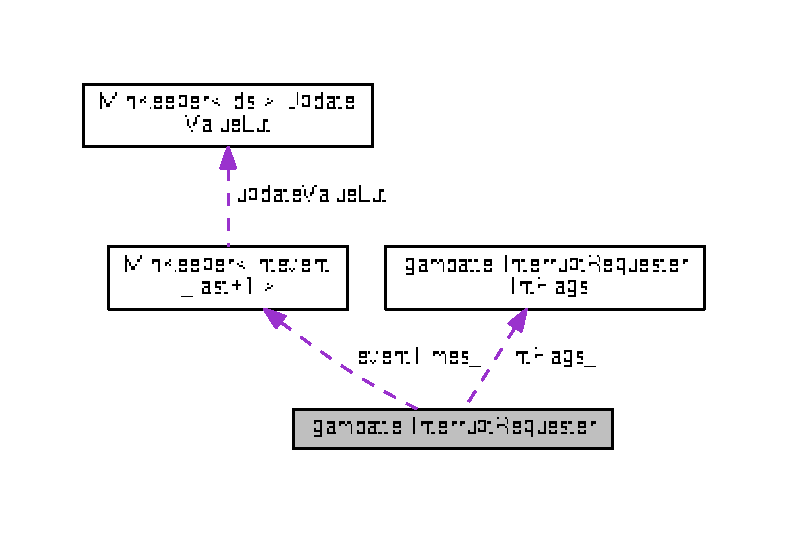
\includegraphics[width=350pt]{classgambatte_1_1InterruptRequester__coll__graph}
\end{center}
\end{figure}
\subsection*{Classes}
\begin{DoxyCompactItemize}
\item 
class \hyperlink{classgambatte_1_1InterruptRequester_1_1IntFlags}{Int\+Flags}
\end{DoxyCompactItemize}
\subsection*{Public Member Functions}
\begin{DoxyCompactItemize}
\item 
\hyperlink{classgambatte_1_1InterruptRequester_a191cbbeafc8cc226515b4940f33f2d5c}{Interrupt\+Requester} ()
\item 
void \hyperlink{classgambatte_1_1InterruptRequester_af5e1e339110d86ead8e883001d570786}{save\+State} (\hyperlink{structgambatte_1_1SaveState}{Save\+State} \&) const
\item 
void \hyperlink{classgambatte_1_1InterruptRequester_a4b7f9fb97eab43529bf0786337ff2c2a}{load\+State} (\hyperlink{structgambatte_1_1SaveState}{Save\+State} const \&)
\item 
void \hyperlink{classgambatte_1_1InterruptRequester_af6af560b1f2024637873ff329650f4a9}{reset\+Cc} (unsigned old\+Cc, unsigned new\+Cc)
\item 
unsigned \hyperlink{classgambatte_1_1InterruptRequester_ab38b7d0628b45719bbd8a4d2d7fd3d10}{ifreg} () const
\item 
unsigned \hyperlink{classgambatte_1_1InterruptRequester_adf3a10120c783480d96f98ef412d5983}{pending\+Irqs} () const
\item 
bool \hyperlink{classgambatte_1_1InterruptRequester_a93023cefcd8053095fc3d287321550fd}{ime} () const
\item 
bool \hyperlink{classgambatte_1_1InterruptRequester_aedfaf9bf197e7572b68b09d63b76c38f}{halted} () const
\item 
void \hyperlink{classgambatte_1_1InterruptRequester_ae1e3c916231a1720342029e2ab9b6be0}{ei} (unsigned cc)
\item 
void \hyperlink{classgambatte_1_1InterruptRequester_a25348c898ee8ed469bb3c20046ac1358}{di} ()
\item 
void \hyperlink{classgambatte_1_1InterruptRequester_ade8e794b316125964403032b0b840140}{halt} ()
\item 
void \hyperlink{classgambatte_1_1InterruptRequester_ae81da10d3c802d61a5ebb1aa54974429}{unhalt} ()
\item 
void \hyperlink{classgambatte_1_1InterruptRequester_ac6158dd97f6eb919dd38f9968483875c}{flag\+Irq} (unsigned bit)
\item 
void \hyperlink{classgambatte_1_1InterruptRequester_ac23ef853545dc64a53613d8bd76784de}{ack\+Irq} (unsigned bit)
\item 
void \hyperlink{classgambatte_1_1InterruptRequester_a84ecf8964b2379a811b4720598b6dc77}{set\+Iereg} (unsigned iereg)
\item 
void \hyperlink{classgambatte_1_1InterruptRequester_aafe73dd416a93e6044ed523072eb88ad}{set\+Ifreg} (unsigned \hyperlink{classgambatte_1_1InterruptRequester_ab38b7d0628b45719bbd8a4d2d7fd3d10}{ifreg})
\item 
void \hyperlink{classgambatte_1_1InterruptRequester_a55d66a6ca415d5bbe25de2b4f19524c9}{load\+Or\+Save} (\hyperlink{classgambatte_1_1loadsave}{loadsave} \&\hyperlink{ppu_8cpp_a2f2eca6997ee7baf8901725ae074d45b}{state})
\item 
\hyperlink{namespacegambatte_a0cc3dd7d4d26f0466e9eeda6242755d9}{Int\+Event\+Id} \hyperlink{classgambatte_1_1InterruptRequester_a252ee2f3d6908c81241a2d91c61198d9}{min\+Event\+Id} () const
\item 
unsigned \hyperlink{classgambatte_1_1InterruptRequester_ae8be681ef0489f392ec8c26080eed3c1}{min\+Event\+Time} () const
\item 
{\footnotesize template$<$Int\+Event\+Id id$>$ }\\void \hyperlink{classgambatte_1_1InterruptRequester_a74dea1d66d0f12cd30b8d40ad3e6d812}{set\+Event\+Time} (unsigned value)
\item 
void \hyperlink{classgambatte_1_1InterruptRequester_a1f89a9625dd3c710a380f83307f5185f}{set\+Event\+Time} (\hyperlink{namespacegambatte_a0cc3dd7d4d26f0466e9eeda6242755d9}{Int\+Event\+Id} id, unsigned value)
\item 
unsigned \hyperlink{classgambatte_1_1InterruptRequester_afbab70746a5eea63178d6fd927b27c18}{event\+Time} (\hyperlink{namespacegambatte_a0cc3dd7d4d26f0466e9eeda6242755d9}{Int\+Event\+Id} id) const
\item 
void \hyperlink{classgambatte_1_1InterruptRequester_a72b191ab4268068e248ab100d6981ea2}{print\+\_\+timing\+\_\+state} (void)
\end{DoxyCompactItemize}
\subsection*{Private Attributes}
\begin{DoxyCompactItemize}
\item 
\hyperlink{classMinKeeper}{Min\+Keeper}$<$ \hyperlink{namespacegambatte_a0cc3dd7d4d26f0466e9eeda6242755d9af6db597bb27febfcaf18fcf03e337906}{intevent\+\_\+last}+1 $>$ \hyperlink{classgambatte_1_1InterruptRequester_a251b9c79fc0a1f8dc05337b332bb5699}{event\+Times\+\_\+}
\item 
unsigned \hyperlink{classgambatte_1_1InterruptRequester_a2bdaa2560a52a5c12a80c470466bc8d0}{min\+Int\+Time\+\_\+}
\item 
unsigned \hyperlink{classgambatte_1_1InterruptRequester_a256e0604b1826e6ec9fc2b0aa9ab5c75}{ifreg\+\_\+}
\item 
unsigned \hyperlink{classgambatte_1_1InterruptRequester_a01927caeb6c58a09540a09eed75a8f4f}{iereg\+\_\+}
\item 
\hyperlink{classgambatte_1_1InterruptRequester_1_1IntFlags}{Int\+Flags} \hyperlink{classgambatte_1_1InterruptRequester_a3aedbf6de456171d28d5718671a5b43c}{int\+Flags\+\_\+}
\end{DoxyCompactItemize}


\subsection{Constructor \& Destructor Documentation}
\mbox{\Hypertarget{classgambatte_1_1InterruptRequester_a191cbbeafc8cc226515b4940f33f2d5c}\label{classgambatte_1_1InterruptRequester_a191cbbeafc8cc226515b4940f33f2d5c}} 
\index{gambatte\+::\+Interrupt\+Requester@{gambatte\+::\+Interrupt\+Requester}!Interrupt\+Requester@{Interrupt\+Requester}}
\index{Interrupt\+Requester@{Interrupt\+Requester}!gambatte\+::\+Interrupt\+Requester@{gambatte\+::\+Interrupt\+Requester}}
\subsubsection{\texorpdfstring{Interrupt\+Requester()}{InterruptRequester()}}
{\footnotesize\ttfamily gambatte\+::\+Interrupt\+Requester\+::\+Interrupt\+Requester (\begin{DoxyParamCaption}{ }\end{DoxyParamCaption})}



\subsection{Member Function Documentation}
\mbox{\Hypertarget{classgambatte_1_1InterruptRequester_ac23ef853545dc64a53613d8bd76784de}\label{classgambatte_1_1InterruptRequester_ac23ef853545dc64a53613d8bd76784de}} 
\index{gambatte\+::\+Interrupt\+Requester@{gambatte\+::\+Interrupt\+Requester}!ack\+Irq@{ack\+Irq}}
\index{ack\+Irq@{ack\+Irq}!gambatte\+::\+Interrupt\+Requester@{gambatte\+::\+Interrupt\+Requester}}
\subsubsection{\texorpdfstring{ack\+Irq()}{ackIrq()}}
{\footnotesize\ttfamily void gambatte\+::\+Interrupt\+Requester\+::ack\+Irq (\begin{DoxyParamCaption}\item[{unsigned}]{bit }\end{DoxyParamCaption})}

\mbox{\Hypertarget{classgambatte_1_1InterruptRequester_a25348c898ee8ed469bb3c20046ac1358}\label{classgambatte_1_1InterruptRequester_a25348c898ee8ed469bb3c20046ac1358}} 
\index{gambatte\+::\+Interrupt\+Requester@{gambatte\+::\+Interrupt\+Requester}!di@{di}}
\index{di@{di}!gambatte\+::\+Interrupt\+Requester@{gambatte\+::\+Interrupt\+Requester}}
\subsubsection{\texorpdfstring{di()}{di()}}
{\footnotesize\ttfamily void gambatte\+::\+Interrupt\+Requester\+::di (\begin{DoxyParamCaption}{ }\end{DoxyParamCaption})}

\mbox{\Hypertarget{classgambatte_1_1InterruptRequester_ae1e3c916231a1720342029e2ab9b6be0}\label{classgambatte_1_1InterruptRequester_ae1e3c916231a1720342029e2ab9b6be0}} 
\index{gambatte\+::\+Interrupt\+Requester@{gambatte\+::\+Interrupt\+Requester}!ei@{ei}}
\index{ei@{ei}!gambatte\+::\+Interrupt\+Requester@{gambatte\+::\+Interrupt\+Requester}}
\subsubsection{\texorpdfstring{ei()}{ei()}}
{\footnotesize\ttfamily void gambatte\+::\+Interrupt\+Requester\+::ei (\begin{DoxyParamCaption}\item[{unsigned}]{cc }\end{DoxyParamCaption})}

\mbox{\Hypertarget{classgambatte_1_1InterruptRequester_afbab70746a5eea63178d6fd927b27c18}\label{classgambatte_1_1InterruptRequester_afbab70746a5eea63178d6fd927b27c18}} 
\index{gambatte\+::\+Interrupt\+Requester@{gambatte\+::\+Interrupt\+Requester}!event\+Time@{event\+Time}}
\index{event\+Time@{event\+Time}!gambatte\+::\+Interrupt\+Requester@{gambatte\+::\+Interrupt\+Requester}}
\subsubsection{\texorpdfstring{event\+Time()}{eventTime()}}
{\footnotesize\ttfamily unsigned gambatte\+::\+Interrupt\+Requester\+::event\+Time (\begin{DoxyParamCaption}\item[{\hyperlink{namespacegambatte_a0cc3dd7d4d26f0466e9eeda6242755d9}{Int\+Event\+Id}}]{id }\end{DoxyParamCaption}) const\hspace{0.3cm}{\ttfamily [inline]}}

\mbox{\Hypertarget{classgambatte_1_1InterruptRequester_ac6158dd97f6eb919dd38f9968483875c}\label{classgambatte_1_1InterruptRequester_ac6158dd97f6eb919dd38f9968483875c}} 
\index{gambatte\+::\+Interrupt\+Requester@{gambatte\+::\+Interrupt\+Requester}!flag\+Irq@{flag\+Irq}}
\index{flag\+Irq@{flag\+Irq}!gambatte\+::\+Interrupt\+Requester@{gambatte\+::\+Interrupt\+Requester}}
\subsubsection{\texorpdfstring{flag\+Irq()}{flagIrq()}}
{\footnotesize\ttfamily void gambatte\+::\+Interrupt\+Requester\+::flag\+Irq (\begin{DoxyParamCaption}\item[{unsigned}]{bit }\end{DoxyParamCaption})}

\mbox{\Hypertarget{classgambatte_1_1InterruptRequester_ade8e794b316125964403032b0b840140}\label{classgambatte_1_1InterruptRequester_ade8e794b316125964403032b0b840140}} 
\index{gambatte\+::\+Interrupt\+Requester@{gambatte\+::\+Interrupt\+Requester}!halt@{halt}}
\index{halt@{halt}!gambatte\+::\+Interrupt\+Requester@{gambatte\+::\+Interrupt\+Requester}}
\subsubsection{\texorpdfstring{halt()}{halt()}}
{\footnotesize\ttfamily void gambatte\+::\+Interrupt\+Requester\+::halt (\begin{DoxyParamCaption}{ }\end{DoxyParamCaption})}

\mbox{\Hypertarget{classgambatte_1_1InterruptRequester_aedfaf9bf197e7572b68b09d63b76c38f}\label{classgambatte_1_1InterruptRequester_aedfaf9bf197e7572b68b09d63b76c38f}} 
\index{gambatte\+::\+Interrupt\+Requester@{gambatte\+::\+Interrupt\+Requester}!halted@{halted}}
\index{halted@{halted}!gambatte\+::\+Interrupt\+Requester@{gambatte\+::\+Interrupt\+Requester}}
\subsubsection{\texorpdfstring{halted()}{halted()}}
{\footnotesize\ttfamily bool gambatte\+::\+Interrupt\+Requester\+::halted (\begin{DoxyParamCaption}{ }\end{DoxyParamCaption}) const\hspace{0.3cm}{\ttfamily [inline]}}

\mbox{\Hypertarget{classgambatte_1_1InterruptRequester_ab38b7d0628b45719bbd8a4d2d7fd3d10}\label{classgambatte_1_1InterruptRequester_ab38b7d0628b45719bbd8a4d2d7fd3d10}} 
\index{gambatte\+::\+Interrupt\+Requester@{gambatte\+::\+Interrupt\+Requester}!ifreg@{ifreg}}
\index{ifreg@{ifreg}!gambatte\+::\+Interrupt\+Requester@{gambatte\+::\+Interrupt\+Requester}}
\subsubsection{\texorpdfstring{ifreg()}{ifreg()}}
{\footnotesize\ttfamily unsigned gambatte\+::\+Interrupt\+Requester\+::ifreg (\begin{DoxyParamCaption}{ }\end{DoxyParamCaption}) const\hspace{0.3cm}{\ttfamily [inline]}}

\mbox{\Hypertarget{classgambatte_1_1InterruptRequester_a93023cefcd8053095fc3d287321550fd}\label{classgambatte_1_1InterruptRequester_a93023cefcd8053095fc3d287321550fd}} 
\index{gambatte\+::\+Interrupt\+Requester@{gambatte\+::\+Interrupt\+Requester}!ime@{ime}}
\index{ime@{ime}!gambatte\+::\+Interrupt\+Requester@{gambatte\+::\+Interrupt\+Requester}}
\subsubsection{\texorpdfstring{ime()}{ime()}}
{\footnotesize\ttfamily bool gambatte\+::\+Interrupt\+Requester\+::ime (\begin{DoxyParamCaption}{ }\end{DoxyParamCaption}) const\hspace{0.3cm}{\ttfamily [inline]}}

\mbox{\Hypertarget{classgambatte_1_1InterruptRequester_a55d66a6ca415d5bbe25de2b4f19524c9}\label{classgambatte_1_1InterruptRequester_a55d66a6ca415d5bbe25de2b4f19524c9}} 
\index{gambatte\+::\+Interrupt\+Requester@{gambatte\+::\+Interrupt\+Requester}!load\+Or\+Save@{load\+Or\+Save}}
\index{load\+Or\+Save@{load\+Or\+Save}!gambatte\+::\+Interrupt\+Requester@{gambatte\+::\+Interrupt\+Requester}}
\subsubsection{\texorpdfstring{load\+Or\+Save()}{loadOrSave()}}
{\footnotesize\ttfamily void gambatte\+::\+Interrupt\+Requester\+::load\+Or\+Save (\begin{DoxyParamCaption}\item[{\hyperlink{classgambatte_1_1loadsave}{loadsave} \&}]{state }\end{DoxyParamCaption})}

\mbox{\Hypertarget{classgambatte_1_1InterruptRequester_a4b7f9fb97eab43529bf0786337ff2c2a}\label{classgambatte_1_1InterruptRequester_a4b7f9fb97eab43529bf0786337ff2c2a}} 
\index{gambatte\+::\+Interrupt\+Requester@{gambatte\+::\+Interrupt\+Requester}!load\+State@{load\+State}}
\index{load\+State@{load\+State}!gambatte\+::\+Interrupt\+Requester@{gambatte\+::\+Interrupt\+Requester}}
\subsubsection{\texorpdfstring{load\+State()}{loadState()}}
{\footnotesize\ttfamily void gambatte\+::\+Interrupt\+Requester\+::load\+State (\begin{DoxyParamCaption}\item[{\hyperlink{structgambatte_1_1SaveState}{Save\+State} const \&}]{state }\end{DoxyParamCaption})}

\mbox{\Hypertarget{classgambatte_1_1InterruptRequester_a252ee2f3d6908c81241a2d91c61198d9}\label{classgambatte_1_1InterruptRequester_a252ee2f3d6908c81241a2d91c61198d9}} 
\index{gambatte\+::\+Interrupt\+Requester@{gambatte\+::\+Interrupt\+Requester}!min\+Event\+Id@{min\+Event\+Id}}
\index{min\+Event\+Id@{min\+Event\+Id}!gambatte\+::\+Interrupt\+Requester@{gambatte\+::\+Interrupt\+Requester}}
\subsubsection{\texorpdfstring{min\+Event\+Id()}{minEventId()}}
{\footnotesize\ttfamily \hyperlink{namespacegambatte_a0cc3dd7d4d26f0466e9eeda6242755d9}{Int\+Event\+Id} gambatte\+::\+Interrupt\+Requester\+::min\+Event\+Id (\begin{DoxyParamCaption}{ }\end{DoxyParamCaption}) const\hspace{0.3cm}{\ttfamily [inline]}}

\mbox{\Hypertarget{classgambatte_1_1InterruptRequester_ae8be681ef0489f392ec8c26080eed3c1}\label{classgambatte_1_1InterruptRequester_ae8be681ef0489f392ec8c26080eed3c1}} 
\index{gambatte\+::\+Interrupt\+Requester@{gambatte\+::\+Interrupt\+Requester}!min\+Event\+Time@{min\+Event\+Time}}
\index{min\+Event\+Time@{min\+Event\+Time}!gambatte\+::\+Interrupt\+Requester@{gambatte\+::\+Interrupt\+Requester}}
\subsubsection{\texorpdfstring{min\+Event\+Time()}{minEventTime()}}
{\footnotesize\ttfamily unsigned gambatte\+::\+Interrupt\+Requester\+::min\+Event\+Time (\begin{DoxyParamCaption}{ }\end{DoxyParamCaption}) const\hspace{0.3cm}{\ttfamily [inline]}}

\mbox{\Hypertarget{classgambatte_1_1InterruptRequester_adf3a10120c783480d96f98ef412d5983}\label{classgambatte_1_1InterruptRequester_adf3a10120c783480d96f98ef412d5983}} 
\index{gambatte\+::\+Interrupt\+Requester@{gambatte\+::\+Interrupt\+Requester}!pending\+Irqs@{pending\+Irqs}}
\index{pending\+Irqs@{pending\+Irqs}!gambatte\+::\+Interrupt\+Requester@{gambatte\+::\+Interrupt\+Requester}}
\subsubsection{\texorpdfstring{pending\+Irqs()}{pendingIrqs()}}
{\footnotesize\ttfamily unsigned gambatte\+::\+Interrupt\+Requester\+::pending\+Irqs (\begin{DoxyParamCaption}{ }\end{DoxyParamCaption}) const\hspace{0.3cm}{\ttfamily [inline]}}

\mbox{\Hypertarget{classgambatte_1_1InterruptRequester_a72b191ab4268068e248ab100d6981ea2}\label{classgambatte_1_1InterruptRequester_a72b191ab4268068e248ab100d6981ea2}} 
\index{gambatte\+::\+Interrupt\+Requester@{gambatte\+::\+Interrupt\+Requester}!print\+\_\+timing\+\_\+state@{print\+\_\+timing\+\_\+state}}
\index{print\+\_\+timing\+\_\+state@{print\+\_\+timing\+\_\+state}!gambatte\+::\+Interrupt\+Requester@{gambatte\+::\+Interrupt\+Requester}}
\subsubsection{\texorpdfstring{print\+\_\+timing\+\_\+state()}{print\_timing\_state()}}
{\footnotesize\ttfamily void gambatte\+::\+Interrupt\+Requester\+::print\+\_\+timing\+\_\+state (\begin{DoxyParamCaption}\item[{void}]{ }\end{DoxyParamCaption})\hspace{0.3cm}{\ttfamily [inline]}}

\mbox{\Hypertarget{classgambatte_1_1InterruptRequester_af6af560b1f2024637873ff329650f4a9}\label{classgambatte_1_1InterruptRequester_af6af560b1f2024637873ff329650f4a9}} 
\index{gambatte\+::\+Interrupt\+Requester@{gambatte\+::\+Interrupt\+Requester}!reset\+Cc@{reset\+Cc}}
\index{reset\+Cc@{reset\+Cc}!gambatte\+::\+Interrupt\+Requester@{gambatte\+::\+Interrupt\+Requester}}
\subsubsection{\texorpdfstring{reset\+Cc()}{resetCc()}}
{\footnotesize\ttfamily void gambatte\+::\+Interrupt\+Requester\+::reset\+Cc (\begin{DoxyParamCaption}\item[{unsigned}]{old\+Cc,  }\item[{unsigned}]{new\+Cc }\end{DoxyParamCaption})}

\mbox{\Hypertarget{classgambatte_1_1InterruptRequester_af5e1e339110d86ead8e883001d570786}\label{classgambatte_1_1InterruptRequester_af5e1e339110d86ead8e883001d570786}} 
\index{gambatte\+::\+Interrupt\+Requester@{gambatte\+::\+Interrupt\+Requester}!save\+State@{save\+State}}
\index{save\+State@{save\+State}!gambatte\+::\+Interrupt\+Requester@{gambatte\+::\+Interrupt\+Requester}}
\subsubsection{\texorpdfstring{save\+State()}{saveState()}}
{\footnotesize\ttfamily void gambatte\+::\+Interrupt\+Requester\+::save\+State (\begin{DoxyParamCaption}\item[{\hyperlink{structgambatte_1_1SaveState}{Save\+State} \&}]{state }\end{DoxyParamCaption}) const}

\mbox{\Hypertarget{classgambatte_1_1InterruptRequester_a74dea1d66d0f12cd30b8d40ad3e6d812}\label{classgambatte_1_1InterruptRequester_a74dea1d66d0f12cd30b8d40ad3e6d812}} 
\index{gambatte\+::\+Interrupt\+Requester@{gambatte\+::\+Interrupt\+Requester}!set\+Event\+Time@{set\+Event\+Time}}
\index{set\+Event\+Time@{set\+Event\+Time}!gambatte\+::\+Interrupt\+Requester@{gambatte\+::\+Interrupt\+Requester}}
\subsubsection{\texorpdfstring{set\+Event\+Time()}{setEventTime()}\hspace{0.1cm}{\footnotesize\ttfamily [1/2]}}
{\footnotesize\ttfamily template$<$Int\+Event\+Id id$>$ \\
void gambatte\+::\+Interrupt\+Requester\+::set\+Event\+Time (\begin{DoxyParamCaption}\item[{unsigned}]{value }\end{DoxyParamCaption})\hspace{0.3cm}{\ttfamily [inline]}}

\mbox{\Hypertarget{classgambatte_1_1InterruptRequester_a1f89a9625dd3c710a380f83307f5185f}\label{classgambatte_1_1InterruptRequester_a1f89a9625dd3c710a380f83307f5185f}} 
\index{gambatte\+::\+Interrupt\+Requester@{gambatte\+::\+Interrupt\+Requester}!set\+Event\+Time@{set\+Event\+Time}}
\index{set\+Event\+Time@{set\+Event\+Time}!gambatte\+::\+Interrupt\+Requester@{gambatte\+::\+Interrupt\+Requester}}
\subsubsection{\texorpdfstring{set\+Event\+Time()}{setEventTime()}\hspace{0.1cm}{\footnotesize\ttfamily [2/2]}}
{\footnotesize\ttfamily void gambatte\+::\+Interrupt\+Requester\+::set\+Event\+Time (\begin{DoxyParamCaption}\item[{\hyperlink{namespacegambatte_a0cc3dd7d4d26f0466e9eeda6242755d9}{Int\+Event\+Id}}]{id,  }\item[{unsigned}]{value }\end{DoxyParamCaption})\hspace{0.3cm}{\ttfamily [inline]}}

\mbox{\Hypertarget{classgambatte_1_1InterruptRequester_a84ecf8964b2379a811b4720598b6dc77}\label{classgambatte_1_1InterruptRequester_a84ecf8964b2379a811b4720598b6dc77}} 
\index{gambatte\+::\+Interrupt\+Requester@{gambatte\+::\+Interrupt\+Requester}!set\+Iereg@{set\+Iereg}}
\index{set\+Iereg@{set\+Iereg}!gambatte\+::\+Interrupt\+Requester@{gambatte\+::\+Interrupt\+Requester}}
\subsubsection{\texorpdfstring{set\+Iereg()}{setIereg()}}
{\footnotesize\ttfamily void gambatte\+::\+Interrupt\+Requester\+::set\+Iereg (\begin{DoxyParamCaption}\item[{unsigned}]{iereg }\end{DoxyParamCaption})}

\mbox{\Hypertarget{classgambatte_1_1InterruptRequester_aafe73dd416a93e6044ed523072eb88ad}\label{classgambatte_1_1InterruptRequester_aafe73dd416a93e6044ed523072eb88ad}} 
\index{gambatte\+::\+Interrupt\+Requester@{gambatte\+::\+Interrupt\+Requester}!set\+Ifreg@{set\+Ifreg}}
\index{set\+Ifreg@{set\+Ifreg}!gambatte\+::\+Interrupt\+Requester@{gambatte\+::\+Interrupt\+Requester}}
\subsubsection{\texorpdfstring{set\+Ifreg()}{setIfreg()}}
{\footnotesize\ttfamily void gambatte\+::\+Interrupt\+Requester\+::set\+Ifreg (\begin{DoxyParamCaption}\item[{unsigned}]{ifreg }\end{DoxyParamCaption})}

\mbox{\Hypertarget{classgambatte_1_1InterruptRequester_ae81da10d3c802d61a5ebb1aa54974429}\label{classgambatte_1_1InterruptRequester_ae81da10d3c802d61a5ebb1aa54974429}} 
\index{gambatte\+::\+Interrupt\+Requester@{gambatte\+::\+Interrupt\+Requester}!unhalt@{unhalt}}
\index{unhalt@{unhalt}!gambatte\+::\+Interrupt\+Requester@{gambatte\+::\+Interrupt\+Requester}}
\subsubsection{\texorpdfstring{unhalt()}{unhalt()}}
{\footnotesize\ttfamily void gambatte\+::\+Interrupt\+Requester\+::unhalt (\begin{DoxyParamCaption}{ }\end{DoxyParamCaption})}



\subsection{Member Data Documentation}
\mbox{\Hypertarget{classgambatte_1_1InterruptRequester_a251b9c79fc0a1f8dc05337b332bb5699}\label{classgambatte_1_1InterruptRequester_a251b9c79fc0a1f8dc05337b332bb5699}} 
\index{gambatte\+::\+Interrupt\+Requester@{gambatte\+::\+Interrupt\+Requester}!event\+Times\+\_\+@{event\+Times\+\_\+}}
\index{event\+Times\+\_\+@{event\+Times\+\_\+}!gambatte\+::\+Interrupt\+Requester@{gambatte\+::\+Interrupt\+Requester}}
\subsubsection{\texorpdfstring{event\+Times\+\_\+}{eventTimes\_}}
{\footnotesize\ttfamily \hyperlink{classMinKeeper}{Min\+Keeper}$<$\hyperlink{namespacegambatte_a0cc3dd7d4d26f0466e9eeda6242755d9af6db597bb27febfcaf18fcf03e337906}{intevent\+\_\+last} + 1$>$ gambatte\+::\+Interrupt\+Requester\+::event\+Times\+\_\+\hspace{0.3cm}{\ttfamily [private]}}

\mbox{\Hypertarget{classgambatte_1_1InterruptRequester_a01927caeb6c58a09540a09eed75a8f4f}\label{classgambatte_1_1InterruptRequester_a01927caeb6c58a09540a09eed75a8f4f}} 
\index{gambatte\+::\+Interrupt\+Requester@{gambatte\+::\+Interrupt\+Requester}!iereg\+\_\+@{iereg\+\_\+}}
\index{iereg\+\_\+@{iereg\+\_\+}!gambatte\+::\+Interrupt\+Requester@{gambatte\+::\+Interrupt\+Requester}}
\subsubsection{\texorpdfstring{iereg\+\_\+}{iereg\_}}
{\footnotesize\ttfamily unsigned gambatte\+::\+Interrupt\+Requester\+::iereg\+\_\+\hspace{0.3cm}{\ttfamily [private]}}

\mbox{\Hypertarget{classgambatte_1_1InterruptRequester_a256e0604b1826e6ec9fc2b0aa9ab5c75}\label{classgambatte_1_1InterruptRequester_a256e0604b1826e6ec9fc2b0aa9ab5c75}} 
\index{gambatte\+::\+Interrupt\+Requester@{gambatte\+::\+Interrupt\+Requester}!ifreg\+\_\+@{ifreg\+\_\+}}
\index{ifreg\+\_\+@{ifreg\+\_\+}!gambatte\+::\+Interrupt\+Requester@{gambatte\+::\+Interrupt\+Requester}}
\subsubsection{\texorpdfstring{ifreg\+\_\+}{ifreg\_}}
{\footnotesize\ttfamily unsigned gambatte\+::\+Interrupt\+Requester\+::ifreg\+\_\+\hspace{0.3cm}{\ttfamily [private]}}

\mbox{\Hypertarget{classgambatte_1_1InterruptRequester_a3aedbf6de456171d28d5718671a5b43c}\label{classgambatte_1_1InterruptRequester_a3aedbf6de456171d28d5718671a5b43c}} 
\index{gambatte\+::\+Interrupt\+Requester@{gambatte\+::\+Interrupt\+Requester}!int\+Flags\+\_\+@{int\+Flags\+\_\+}}
\index{int\+Flags\+\_\+@{int\+Flags\+\_\+}!gambatte\+::\+Interrupt\+Requester@{gambatte\+::\+Interrupt\+Requester}}
\subsubsection{\texorpdfstring{int\+Flags\+\_\+}{intFlags\_}}
{\footnotesize\ttfamily \hyperlink{classgambatte_1_1InterruptRequester_1_1IntFlags}{Int\+Flags} gambatte\+::\+Interrupt\+Requester\+::int\+Flags\+\_\+\hspace{0.3cm}{\ttfamily [private]}}

\mbox{\Hypertarget{classgambatte_1_1InterruptRequester_a2bdaa2560a52a5c12a80c470466bc8d0}\label{classgambatte_1_1InterruptRequester_a2bdaa2560a52a5c12a80c470466bc8d0}} 
\index{gambatte\+::\+Interrupt\+Requester@{gambatte\+::\+Interrupt\+Requester}!min\+Int\+Time\+\_\+@{min\+Int\+Time\+\_\+}}
\index{min\+Int\+Time\+\_\+@{min\+Int\+Time\+\_\+}!gambatte\+::\+Interrupt\+Requester@{gambatte\+::\+Interrupt\+Requester}}
\subsubsection{\texorpdfstring{min\+Int\+Time\+\_\+}{minIntTime\_}}
{\footnotesize\ttfamily unsigned gambatte\+::\+Interrupt\+Requester\+::min\+Int\+Time\+\_\+\hspace{0.3cm}{\ttfamily [private]}}



The documentation for this class was generated from the following files\+:\begin{DoxyCompactItemize}
\item 
src/\hyperlink{interruptrequester_8h}{interruptrequester.\+h}\item 
src/\hyperlink{interruptrequester_8cpp}{interruptrequester.\+cpp}\end{DoxyCompactItemize}

\hypertarget{classgambatte_1_1InterruptRequester_1_1IntFlags}{}\section{gambatte\+:\+:Interrupt\+Requester\+:\+:Int\+Flags Class Reference}
\label{classgambatte_1_1InterruptRequester_1_1IntFlags}\index{gambatte\+::\+Interrupt\+Requester\+::\+Int\+Flags@{gambatte\+::\+Interrupt\+Requester\+::\+Int\+Flags}}
\subsection*{Public Member Functions}
\begin{DoxyCompactItemize}
\item 
\hyperlink{classgambatte_1_1InterruptRequester_1_1IntFlags_ade4bb1590cd0d09681771bfd5c14162c}{Int\+Flags} ()
\item 
bool \hyperlink{classgambatte_1_1InterruptRequester_1_1IntFlags_a1d2013209732079b1808306088d931ff}{ime} () const
\item 
bool \hyperlink{classgambatte_1_1InterruptRequester_1_1IntFlags_a8206d665f9772d64144d6be5d8c1a5cb}{halted} () const
\item 
bool \hyperlink{classgambatte_1_1InterruptRequester_1_1IntFlags_a8fa10e667caf8ee75e4160831b408e5f}{ime\+Or\+Halted} () const
\item 
void \hyperlink{classgambatte_1_1InterruptRequester_1_1IntFlags_a7ba10cdfb4510071d25d34f156f0d340}{set\+Ime} ()
\item 
void \hyperlink{classgambatte_1_1InterruptRequester_1_1IntFlags_a200fcbd2f4aafc8d1270f127f6b73605}{unset\+Ime} ()
\item 
void \hyperlink{classgambatte_1_1InterruptRequester_1_1IntFlags_a1165e408af70f4c57bad2624aca64c91}{set\+Halted} ()
\item 
void \hyperlink{classgambatte_1_1InterruptRequester_1_1IntFlags_ab8a9985dc5e4319aae2604e82948f2ed}{unset\+Halted} ()
\item 
void \hyperlink{classgambatte_1_1InterruptRequester_1_1IntFlags_a39bae600579578159fd4479a7db8bffd}{set} (bool \hyperlink{classgambatte_1_1InterruptRequester_1_1IntFlags_a1d2013209732079b1808306088d931ff}{ime}, bool \hyperlink{classgambatte_1_1InterruptRequester_1_1IntFlags_a8206d665f9772d64144d6be5d8c1a5cb}{halted})
\item 
void \hyperlink{classgambatte_1_1InterruptRequester_1_1IntFlags_a67e0b21fe08af2364e644b6240fe28d3}{load\+Or\+Save} (\hyperlink{classgambatte_1_1loadsave}{loadsave} \&\hyperlink{ppu_8cpp_a2f2eca6997ee7baf8901725ae074d45b}{state})
\end{DoxyCompactItemize}
\subsection*{Private Types}
\begin{DoxyCompactItemize}
\item 
enum \{ \hyperlink{classgambatte_1_1InterruptRequester_1_1IntFlags_ac12aff71731b6bee64b7d9904eab9d61ac0e5e5336630c11283f53c3b62456b10}{flag\+\_\+ime} = 1, 
\hyperlink{classgambatte_1_1InterruptRequester_1_1IntFlags_ac12aff71731b6bee64b7d9904eab9d61a6a6552113ff0fc08e8a0d684d1c2e920}{flag\+\_\+halted} = 2
 \}
\end{DoxyCompactItemize}
\subsection*{Private Attributes}
\begin{DoxyCompactItemize}
\item 
unsigned char \hyperlink{classgambatte_1_1InterruptRequester_1_1IntFlags_ada70b74691d5e79f664bf956dc1eeadc}{flags\+\_\+}
\end{DoxyCompactItemize}


\subsection{Member Enumeration Documentation}
\mbox{\Hypertarget{classgambatte_1_1InterruptRequester_1_1IntFlags_ac12aff71731b6bee64b7d9904eab9d61}\label{classgambatte_1_1InterruptRequester_1_1IntFlags_ac12aff71731b6bee64b7d9904eab9d61}} 
\subsubsection{\texorpdfstring{anonymous enum}{anonymous enum}}
{\footnotesize\ttfamily anonymous enum\hspace{0.3cm}{\ttfamily [private]}}

\begin{DoxyEnumFields}{Enumerator}
\raisebox{\heightof{T}}[0pt][0pt]{\index{flag\+\_\+ime@{flag\+\_\+ime}!gambatte\+::\+Interrupt\+Requester\+::\+Int\+Flags@{gambatte\+::\+Interrupt\+Requester\+::\+Int\+Flags}}\index{gambatte\+::\+Interrupt\+Requester\+::\+Int\+Flags@{gambatte\+::\+Interrupt\+Requester\+::\+Int\+Flags}!flag\+\_\+ime@{flag\+\_\+ime}}}\mbox{\Hypertarget{classgambatte_1_1InterruptRequester_1_1IntFlags_ac12aff71731b6bee64b7d9904eab9d61ac0e5e5336630c11283f53c3b62456b10}\label{classgambatte_1_1InterruptRequester_1_1IntFlags_ac12aff71731b6bee64b7d9904eab9d61ac0e5e5336630c11283f53c3b62456b10}} 
flag\+\_\+ime&\\
\hline

\raisebox{\heightof{T}}[0pt][0pt]{\index{flag\+\_\+halted@{flag\+\_\+halted}!gambatte\+::\+Interrupt\+Requester\+::\+Int\+Flags@{gambatte\+::\+Interrupt\+Requester\+::\+Int\+Flags}}\index{gambatte\+::\+Interrupt\+Requester\+::\+Int\+Flags@{gambatte\+::\+Interrupt\+Requester\+::\+Int\+Flags}!flag\+\_\+halted@{flag\+\_\+halted}}}\mbox{\Hypertarget{classgambatte_1_1InterruptRequester_1_1IntFlags_ac12aff71731b6bee64b7d9904eab9d61a6a6552113ff0fc08e8a0d684d1c2e920}\label{classgambatte_1_1InterruptRequester_1_1IntFlags_ac12aff71731b6bee64b7d9904eab9d61a6a6552113ff0fc08e8a0d684d1c2e920}} 
flag\+\_\+halted&\\
\hline

\end{DoxyEnumFields}


\subsection{Constructor \& Destructor Documentation}
\mbox{\Hypertarget{classgambatte_1_1InterruptRequester_1_1IntFlags_ade4bb1590cd0d09681771bfd5c14162c}\label{classgambatte_1_1InterruptRequester_1_1IntFlags_ade4bb1590cd0d09681771bfd5c14162c}} 
\index{gambatte\+::\+Interrupt\+Requester\+::\+Int\+Flags@{gambatte\+::\+Interrupt\+Requester\+::\+Int\+Flags}!Int\+Flags@{Int\+Flags}}
\index{Int\+Flags@{Int\+Flags}!gambatte\+::\+Interrupt\+Requester\+::\+Int\+Flags@{gambatte\+::\+Interrupt\+Requester\+::\+Int\+Flags}}
\subsubsection{\texorpdfstring{Int\+Flags()}{IntFlags()}}
{\footnotesize\ttfamily gambatte\+::\+Interrupt\+Requester\+::\+Int\+Flags\+::\+Int\+Flags (\begin{DoxyParamCaption}{ }\end{DoxyParamCaption})\hspace{0.3cm}{\ttfamily [inline]}}



\subsection{Member Function Documentation}
\mbox{\Hypertarget{classgambatte_1_1InterruptRequester_1_1IntFlags_a8206d665f9772d64144d6be5d8c1a5cb}\label{classgambatte_1_1InterruptRequester_1_1IntFlags_a8206d665f9772d64144d6be5d8c1a5cb}} 
\index{gambatte\+::\+Interrupt\+Requester\+::\+Int\+Flags@{gambatte\+::\+Interrupt\+Requester\+::\+Int\+Flags}!halted@{halted}}
\index{halted@{halted}!gambatte\+::\+Interrupt\+Requester\+::\+Int\+Flags@{gambatte\+::\+Interrupt\+Requester\+::\+Int\+Flags}}
\subsubsection{\texorpdfstring{halted()}{halted()}}
{\footnotesize\ttfamily bool gambatte\+::\+Interrupt\+Requester\+::\+Int\+Flags\+::halted (\begin{DoxyParamCaption}{ }\end{DoxyParamCaption}) const\hspace{0.3cm}{\ttfamily [inline]}}

\mbox{\Hypertarget{classgambatte_1_1InterruptRequester_1_1IntFlags_a1d2013209732079b1808306088d931ff}\label{classgambatte_1_1InterruptRequester_1_1IntFlags_a1d2013209732079b1808306088d931ff}} 
\index{gambatte\+::\+Interrupt\+Requester\+::\+Int\+Flags@{gambatte\+::\+Interrupt\+Requester\+::\+Int\+Flags}!ime@{ime}}
\index{ime@{ime}!gambatte\+::\+Interrupt\+Requester\+::\+Int\+Flags@{gambatte\+::\+Interrupt\+Requester\+::\+Int\+Flags}}
\subsubsection{\texorpdfstring{ime()}{ime()}}
{\footnotesize\ttfamily bool gambatte\+::\+Interrupt\+Requester\+::\+Int\+Flags\+::ime (\begin{DoxyParamCaption}{ }\end{DoxyParamCaption}) const\hspace{0.3cm}{\ttfamily [inline]}}

\mbox{\Hypertarget{classgambatte_1_1InterruptRequester_1_1IntFlags_a8fa10e667caf8ee75e4160831b408e5f}\label{classgambatte_1_1InterruptRequester_1_1IntFlags_a8fa10e667caf8ee75e4160831b408e5f}} 
\index{gambatte\+::\+Interrupt\+Requester\+::\+Int\+Flags@{gambatte\+::\+Interrupt\+Requester\+::\+Int\+Flags}!ime\+Or\+Halted@{ime\+Or\+Halted}}
\index{ime\+Or\+Halted@{ime\+Or\+Halted}!gambatte\+::\+Interrupt\+Requester\+::\+Int\+Flags@{gambatte\+::\+Interrupt\+Requester\+::\+Int\+Flags}}
\subsubsection{\texorpdfstring{ime\+Or\+Halted()}{imeOrHalted()}}
{\footnotesize\ttfamily bool gambatte\+::\+Interrupt\+Requester\+::\+Int\+Flags\+::ime\+Or\+Halted (\begin{DoxyParamCaption}{ }\end{DoxyParamCaption}) const\hspace{0.3cm}{\ttfamily [inline]}}

\mbox{\Hypertarget{classgambatte_1_1InterruptRequester_1_1IntFlags_a67e0b21fe08af2364e644b6240fe28d3}\label{classgambatte_1_1InterruptRequester_1_1IntFlags_a67e0b21fe08af2364e644b6240fe28d3}} 
\index{gambatte\+::\+Interrupt\+Requester\+::\+Int\+Flags@{gambatte\+::\+Interrupt\+Requester\+::\+Int\+Flags}!load\+Or\+Save@{load\+Or\+Save}}
\index{load\+Or\+Save@{load\+Or\+Save}!gambatte\+::\+Interrupt\+Requester\+::\+Int\+Flags@{gambatte\+::\+Interrupt\+Requester\+::\+Int\+Flags}}
\subsubsection{\texorpdfstring{load\+Or\+Save()}{loadOrSave()}}
{\footnotesize\ttfamily void gambatte\+::\+Interrupt\+Requester\+::\+Int\+Flags\+::load\+Or\+Save (\begin{DoxyParamCaption}\item[{\hyperlink{classgambatte_1_1loadsave}{loadsave} \&}]{state }\end{DoxyParamCaption})\hspace{0.3cm}{\ttfamily [inline]}}

\mbox{\Hypertarget{classgambatte_1_1InterruptRequester_1_1IntFlags_a39bae600579578159fd4479a7db8bffd}\label{classgambatte_1_1InterruptRequester_1_1IntFlags_a39bae600579578159fd4479a7db8bffd}} 
\index{gambatte\+::\+Interrupt\+Requester\+::\+Int\+Flags@{gambatte\+::\+Interrupt\+Requester\+::\+Int\+Flags}!set@{set}}
\index{set@{set}!gambatte\+::\+Interrupt\+Requester\+::\+Int\+Flags@{gambatte\+::\+Interrupt\+Requester\+::\+Int\+Flags}}
\subsubsection{\texorpdfstring{set()}{set()}}
{\footnotesize\ttfamily void gambatte\+::\+Interrupt\+Requester\+::\+Int\+Flags\+::set (\begin{DoxyParamCaption}\item[{bool}]{ime,  }\item[{bool}]{halted }\end{DoxyParamCaption})\hspace{0.3cm}{\ttfamily [inline]}}

\mbox{\Hypertarget{classgambatte_1_1InterruptRequester_1_1IntFlags_a1165e408af70f4c57bad2624aca64c91}\label{classgambatte_1_1InterruptRequester_1_1IntFlags_a1165e408af70f4c57bad2624aca64c91}} 
\index{gambatte\+::\+Interrupt\+Requester\+::\+Int\+Flags@{gambatte\+::\+Interrupt\+Requester\+::\+Int\+Flags}!set\+Halted@{set\+Halted}}
\index{set\+Halted@{set\+Halted}!gambatte\+::\+Interrupt\+Requester\+::\+Int\+Flags@{gambatte\+::\+Interrupt\+Requester\+::\+Int\+Flags}}
\subsubsection{\texorpdfstring{set\+Halted()}{setHalted()}}
{\footnotesize\ttfamily void gambatte\+::\+Interrupt\+Requester\+::\+Int\+Flags\+::set\+Halted (\begin{DoxyParamCaption}{ }\end{DoxyParamCaption})\hspace{0.3cm}{\ttfamily [inline]}}

\mbox{\Hypertarget{classgambatte_1_1InterruptRequester_1_1IntFlags_a7ba10cdfb4510071d25d34f156f0d340}\label{classgambatte_1_1InterruptRequester_1_1IntFlags_a7ba10cdfb4510071d25d34f156f0d340}} 
\index{gambatte\+::\+Interrupt\+Requester\+::\+Int\+Flags@{gambatte\+::\+Interrupt\+Requester\+::\+Int\+Flags}!set\+Ime@{set\+Ime}}
\index{set\+Ime@{set\+Ime}!gambatte\+::\+Interrupt\+Requester\+::\+Int\+Flags@{gambatte\+::\+Interrupt\+Requester\+::\+Int\+Flags}}
\subsubsection{\texorpdfstring{set\+Ime()}{setIme()}}
{\footnotesize\ttfamily void gambatte\+::\+Interrupt\+Requester\+::\+Int\+Flags\+::set\+Ime (\begin{DoxyParamCaption}{ }\end{DoxyParamCaption})\hspace{0.3cm}{\ttfamily [inline]}}

\mbox{\Hypertarget{classgambatte_1_1InterruptRequester_1_1IntFlags_ab8a9985dc5e4319aae2604e82948f2ed}\label{classgambatte_1_1InterruptRequester_1_1IntFlags_ab8a9985dc5e4319aae2604e82948f2ed}} 
\index{gambatte\+::\+Interrupt\+Requester\+::\+Int\+Flags@{gambatte\+::\+Interrupt\+Requester\+::\+Int\+Flags}!unset\+Halted@{unset\+Halted}}
\index{unset\+Halted@{unset\+Halted}!gambatte\+::\+Interrupt\+Requester\+::\+Int\+Flags@{gambatte\+::\+Interrupt\+Requester\+::\+Int\+Flags}}
\subsubsection{\texorpdfstring{unset\+Halted()}{unsetHalted()}}
{\footnotesize\ttfamily void gambatte\+::\+Interrupt\+Requester\+::\+Int\+Flags\+::unset\+Halted (\begin{DoxyParamCaption}{ }\end{DoxyParamCaption})\hspace{0.3cm}{\ttfamily [inline]}}

\mbox{\Hypertarget{classgambatte_1_1InterruptRequester_1_1IntFlags_a200fcbd2f4aafc8d1270f127f6b73605}\label{classgambatte_1_1InterruptRequester_1_1IntFlags_a200fcbd2f4aafc8d1270f127f6b73605}} 
\index{gambatte\+::\+Interrupt\+Requester\+::\+Int\+Flags@{gambatte\+::\+Interrupt\+Requester\+::\+Int\+Flags}!unset\+Ime@{unset\+Ime}}
\index{unset\+Ime@{unset\+Ime}!gambatte\+::\+Interrupt\+Requester\+::\+Int\+Flags@{gambatte\+::\+Interrupt\+Requester\+::\+Int\+Flags}}
\subsubsection{\texorpdfstring{unset\+Ime()}{unsetIme()}}
{\footnotesize\ttfamily void gambatte\+::\+Interrupt\+Requester\+::\+Int\+Flags\+::unset\+Ime (\begin{DoxyParamCaption}{ }\end{DoxyParamCaption})\hspace{0.3cm}{\ttfamily [inline]}}



\subsection{Member Data Documentation}
\mbox{\Hypertarget{classgambatte_1_1InterruptRequester_1_1IntFlags_ada70b74691d5e79f664bf956dc1eeadc}\label{classgambatte_1_1InterruptRequester_1_1IntFlags_ada70b74691d5e79f664bf956dc1eeadc}} 
\index{gambatte\+::\+Interrupt\+Requester\+::\+Int\+Flags@{gambatte\+::\+Interrupt\+Requester\+::\+Int\+Flags}!flags\+\_\+@{flags\+\_\+}}
\index{flags\+\_\+@{flags\+\_\+}!gambatte\+::\+Interrupt\+Requester\+::\+Int\+Flags@{gambatte\+::\+Interrupt\+Requester\+::\+Int\+Flags}}
\subsubsection{\texorpdfstring{flags\+\_\+}{flags\_}}
{\footnotesize\ttfamily unsigned char gambatte\+::\+Interrupt\+Requester\+::\+Int\+Flags\+::flags\+\_\+\hspace{0.3cm}{\ttfamily [private]}}



The documentation for this class was generated from the following file\+:\begin{DoxyCompactItemize}
\item 
src/\hyperlink{interruptrequester_8h}{interruptrequester.\+h}\end{DoxyCompactItemize}

\hypertarget{classgambatte_1_1LCD}{}\section{gambatte\+:\+:L\+CD Class Reference}
\label{classgambatte_1_1LCD}\index{gambatte\+::\+L\+CD@{gambatte\+::\+L\+CD}}


{\ttfamily \#include $<$video.\+h$>$}



Collaboration diagram for gambatte\+:\+:L\+CD\+:
\nopagebreak
\begin{figure}[H]
\begin{center}
\leavevmode
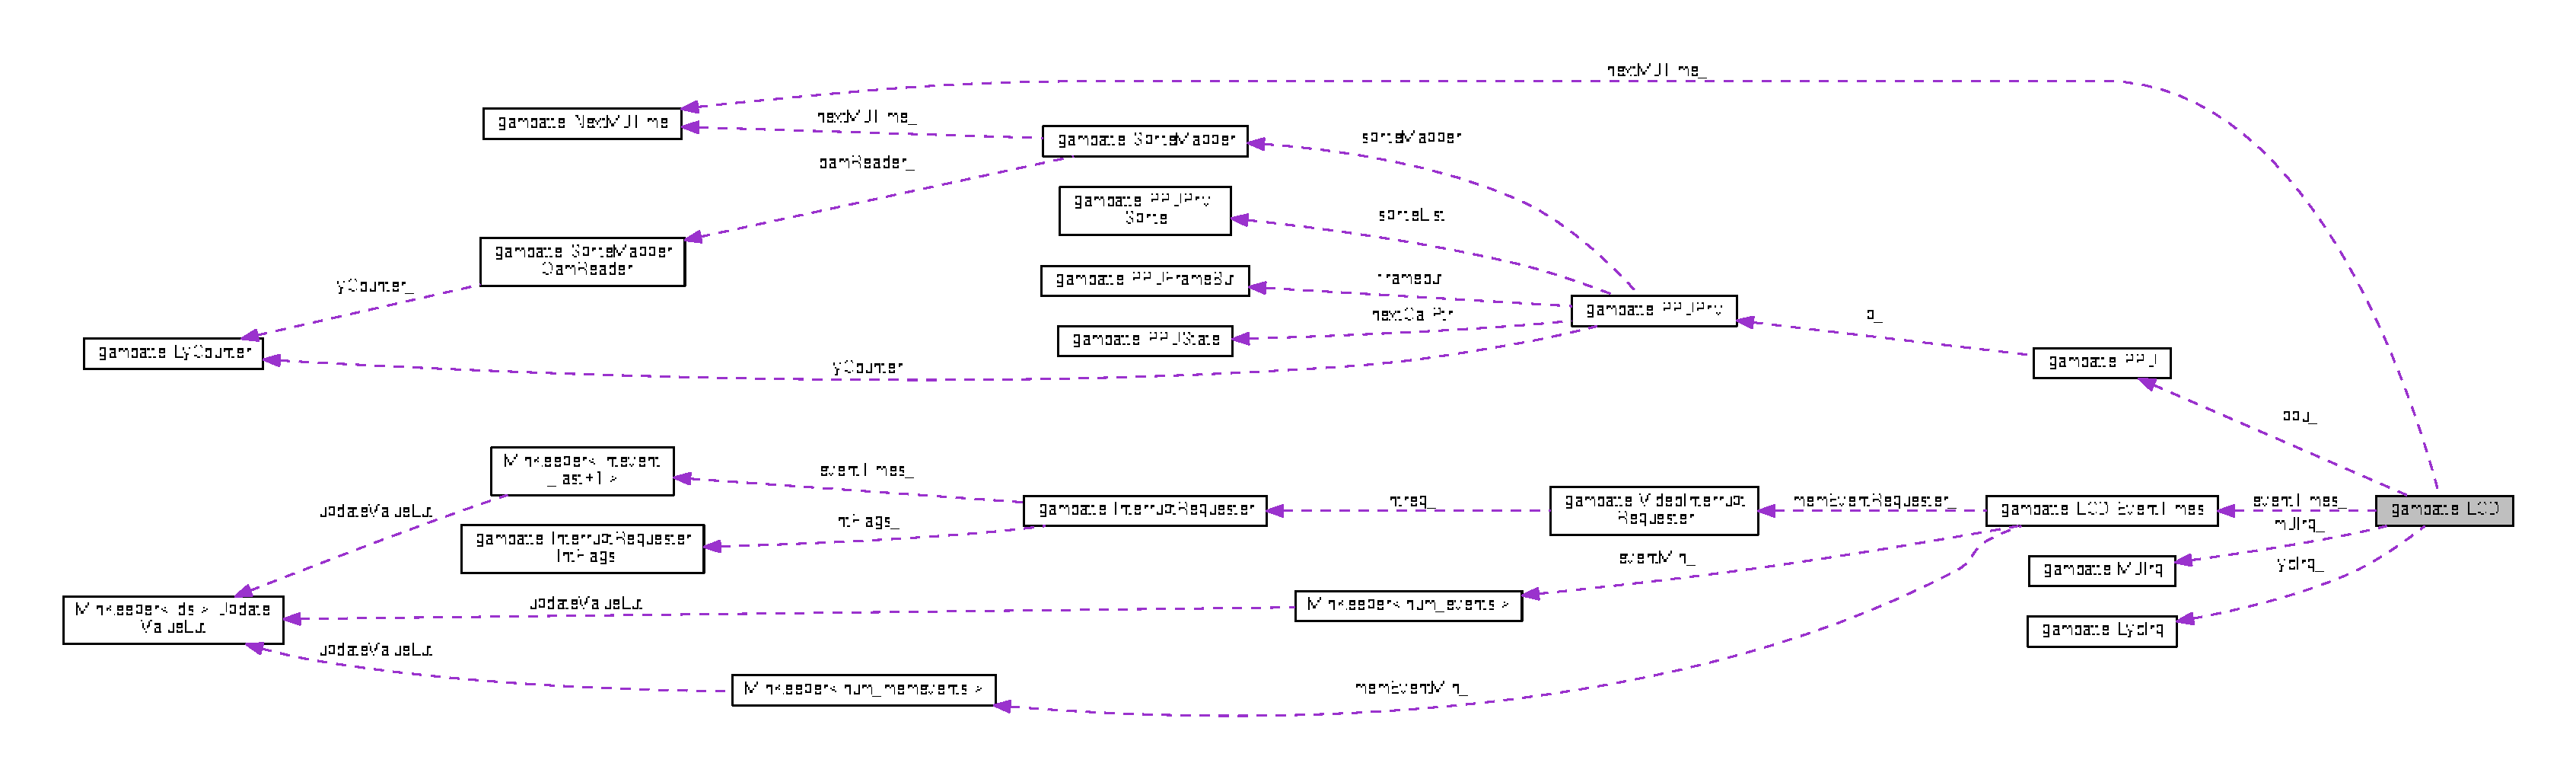
\includegraphics[width=350pt]{classgambatte_1_1LCD__coll__graph}
\end{center}
\end{figure}
\subsection*{Classes}
\begin{DoxyCompactItemize}
\item 
class \hyperlink{classgambatte_1_1LCD_1_1EventTimes}{Event\+Times}
\end{DoxyCompactItemize}
\subsection*{Public Member Functions}
\begin{DoxyCompactItemize}
\item 
\hyperlink{classgambatte_1_1LCD_a27e5f50cbdc1381331be589e35d06650}{L\+CD} (unsigned char const $\ast$oamram, unsigned char const $\ast$vram, \hyperlink{classgambatte_1_1VideoInterruptRequester}{Video\+Interrupt\+Requester} mem\+Event\+Requester)
\item 
void \hyperlink{classgambatte_1_1LCD_a91d74117a2d391d7fab9edc40083531b}{reset} (unsigned char const $\ast$oamram, unsigned char const $\ast$vram, bool cgb)
\item 
void \hyperlink{classgambatte_1_1LCD_ad5525500b675e02a9245ec727b13529c}{set\+State\+Ptrs} (\hyperlink{structgambatte_1_1SaveState}{Save\+State} \&\hyperlink{ppu_8cpp_a2f2eca6997ee7baf8901725ae074d45b}{state})
\item 
void \hyperlink{classgambatte_1_1LCD_a26c4d435be473121e49887c692df9929}{save\+State} (\hyperlink{structgambatte_1_1SaveState}{Save\+State} \&\hyperlink{ppu_8cpp_a2f2eca6997ee7baf8901725ae074d45b}{state}) const
\item 
void \hyperlink{classgambatte_1_1LCD_a516d73f82da6e3908ac8a9fc6899effc}{load\+Or\+Save} (\hyperlink{classgambatte_1_1loadsave}{loadsave} \&\hyperlink{ppu_8cpp_a2f2eca6997ee7baf8901725ae074d45b}{state})
\item 
void \hyperlink{classgambatte_1_1LCD_a9cd3dc21fda725807416ef6b48535f07}{load\+State} (\hyperlink{structgambatte_1_1SaveState}{Save\+State} const \&\hyperlink{ppu_8cpp_a2f2eca6997ee7baf8901725ae074d45b}{state}, unsigned char const $\ast$oamram)
\item 
void \hyperlink{classgambatte_1_1LCD_a824214d860aa4220cb3d058916336261}{set\+Dmg\+Palette\+Color} (unsigned pal\+Num, unsigned color\+Num, \hyperlink{namespacegambatte_a0639f09fccfbbd5a8e0796318768e370}{uint\+\_\+least32\+\_\+t} rgb32)
\item 
void \hyperlink{classgambatte_1_1LCD_a14411e312354ba1d703ae7f6746c431f}{set\+Osd\+Element} (transfer\+\_\+ptr$<$ \hyperlink{classgambatte_1_1OsdElement}{Osd\+Element} $>$ osd\+Element)
\item 
void \hyperlink{classgambatte_1_1LCD_a318d43c9f52b40ee4201fc2838c3661e}{dmg\+Bg\+Palette\+Change} (unsigned data, unsigned cycle\+Counter)
\item 
void \hyperlink{classgambatte_1_1LCD_a3f6a486f4432e89a8a30ac819c0fa437}{dmg\+Sp\+Palette1\+Change} (unsigned data, unsigned cycle\+Counter)
\item 
void \hyperlink{classgambatte_1_1LCD_a2d6e69c85960561020bac66118bad859}{dmg\+Sp\+Palette2\+Change} (unsigned data, unsigned cycle\+Counter)
\item 
void \hyperlink{classgambatte_1_1LCD_a27150bfc8eab3ebf11dbba1282732517}{cgb\+Bg\+Color\+Change} (unsigned index, unsigned data, unsigned cycle\+Counter)
\item 
void \hyperlink{classgambatte_1_1LCD_ac8f3835b4821fbb87c35e2dd2d3b7498}{cgb\+Sp\+Color\+Change} (unsigned index, unsigned data, unsigned cycle\+Counter)
\item 
unsigned \hyperlink{classgambatte_1_1LCD_ae59d87cfa4dbe74cb59678fc2ebe2cc6}{cgb\+Bg\+Color\+Read} (unsigned index, unsigned cycle\+Counter)
\item 
unsigned \hyperlink{classgambatte_1_1LCD_a2fee3de77d90fa6d4316583385d4ee58}{cgb\+Sp\+Color\+Read} (unsigned index, unsigned cycle\+Counter)
\item 
void \hyperlink{classgambatte_1_1LCD_a6a057feecd6cf79fd09ce19ae91e11df}{update\+Screen} (bool blanklcd, unsigned cc, \hyperlink{namespacegambatte_a0639f09fccfbbd5a8e0796318768e370}{uint\+\_\+least32\+\_\+t} $\ast$vbuffer, unsigned vpitch)
\item 
void \hyperlink{classgambatte_1_1LCD_a94ef057d9f530884b5b66bab3a4a5500}{reset\+Cc} (unsigned old\+CC, unsigned new\+Cc)
\item 
void \hyperlink{classgambatte_1_1LCD_a0063fd56fea8f943c2033303e9cdc82b}{speed\+Change} (unsigned cycle\+Counter)
\item 
bool \hyperlink{classgambatte_1_1LCD_a3c94a2934259825fc8e54759aed4c7e5}{vram\+Accessible} (unsigned cycle\+Counter)
\item 
bool \hyperlink{classgambatte_1_1LCD_ac85da77238c2253e877f27ba3cc731c0}{oam\+Readable} (unsigned cycle\+Counter)
\item 
bool \hyperlink{classgambatte_1_1LCD_af0aafdd260473bbe749518838150240c}{oam\+Writable} (unsigned cycle\+Counter)
\item 
void \hyperlink{classgambatte_1_1LCD_ae935760f2500448e0178d99f24aa971a}{wx\+Change} (unsigned new\+Value, unsigned cycle\+Counter)
\item 
void \hyperlink{classgambatte_1_1LCD_a1e9b5824cab29aa84d2af1ff6431dd3e}{wy\+Change} (unsigned new\+Value, unsigned cycle\+Counter)
\item 
void \hyperlink{classgambatte_1_1LCD_a176a351682dbee928b2cbcd29236e2d2}{oam\+Change} (unsigned cycle\+Counter)
\item 
void \hyperlink{classgambatte_1_1LCD_a2198ab07a1eb038f820141c39c312baa}{oam\+Change} (const unsigned char $\ast$oamram, unsigned cycle\+Counter)
\item 
void \hyperlink{classgambatte_1_1LCD_aaac41f27fac136de6a13d7f92ccf64fa}{scx\+Change} (unsigned new\+Scx, unsigned cycle\+Counter)
\item 
void \hyperlink{classgambatte_1_1LCD_a50d315bf6aa30e6405fa0c9ff92494f2}{scy\+Change} (unsigned new\+Value, unsigned cycle\+Counter)
\item 
void \hyperlink{classgambatte_1_1LCD_a3ccafb8445bec07467e96f7bb52c6db9}{vram\+Change} (unsigned cycle\+Counter)
\item 
unsigned \hyperlink{classgambatte_1_1LCD_a547519b1c436bcc02eef931c6cab72db}{get\+Stat} (unsigned lyc\+Reg, unsigned cycle\+Counter)
\item 
unsigned \hyperlink{classgambatte_1_1LCD_a666684dc42954d168509c1b279823607}{get\+Ly\+Reg} (unsigned const cc)
\item 
unsigned \hyperlink{classgambatte_1_1LCD_a9e4fc2713092218b47440166325ef0ca}{next\+Mode1\+Irq\+Time} () const
\item 
void \hyperlink{classgambatte_1_1LCD_a33575ec173dc95fecf92c4e0a0ae6531}{lcdc\+Change} (unsigned data, unsigned cycle\+Counter)
\item 
void \hyperlink{classgambatte_1_1LCD_ade4979ec2f00ae8201c30a83020b289d}{lcdstat\+Change} (unsigned data, unsigned cycle\+Counter)
\item 
void \hyperlink{classgambatte_1_1LCD_a92e048c713983a217e35060dd8f50556}{lyc\+Reg\+Change} (unsigned data, unsigned cycle\+Counter)
\item 
void \hyperlink{classgambatte_1_1LCD_a86dc5a20358fa465677c0735f88b8dca}{enable\+Hdma} (unsigned cycle\+Counter)
\item 
void \hyperlink{classgambatte_1_1LCD_a2e786aa0588f0a1ce49aa602c07a61e3}{disable\+Hdma} (unsigned cycle\+Counter)
\item 
bool \hyperlink{classgambatte_1_1LCD_a9eeebbc4225c4fc1b3893d0373d3d315}{hdma\+Is\+Enabled} () const
\item 
void \hyperlink{classgambatte_1_1LCD_a457f2dd7c97b98c35fc196a1a4259d7c}{update} (unsigned cycle\+Counter)
\item 
bool \hyperlink{classgambatte_1_1LCD_a6e2891b1172f88fd84ce0d15250e35db}{is\+Cgb} () const
\item 
bool \hyperlink{classgambatte_1_1LCD_a603015bdd0d5fdb40f60d3b678706232}{is\+Double\+Speed} () const
\end{DoxyCompactItemize}
\subsection*{Private Types}
\begin{DoxyCompactItemize}
\item 
enum \hyperlink{classgambatte_1_1LCD_a30ec19ea638b75c5c8972b2a1838b0c7}{Event} \{ \hyperlink{classgambatte_1_1LCD_a30ec19ea638b75c5c8972b2a1838b0c7a09337d2a5a8644d6ea771f09e91e2f95}{event\+\_\+mem}, 
\hyperlink{classgambatte_1_1LCD_a30ec19ea638b75c5c8972b2a1838b0c7a438f7b7bf4bd3d362a15fa8e26082ff3}{event\+\_\+ly}, 
\hyperlink{classgambatte_1_1LCD_a30ec19ea638b75c5c8972b2a1838b0c7a06c7c948d55d9363df5976bd712346f6}{event\+\_\+last} = event\+\_\+ly
 \}
\item 
enum \hyperlink{classgambatte_1_1LCD_a71147bde8c21c12e3cb7c70fcab81b76}{Mem\+Event} \{ \newline
\hyperlink{classgambatte_1_1LCD_a71147bde8c21c12e3cb7c70fcab81b76a1c6425619ee45a111c3e534167e6f216}{memevent\+\_\+oneshot\+\_\+statirq}, 
\hyperlink{classgambatte_1_1LCD_a71147bde8c21c12e3cb7c70fcab81b76ae11717075ce3b516d8913ecde6c8854c}{memevent\+\_\+oneshot\+\_\+updatewy2}, 
\hyperlink{classgambatte_1_1LCD_a71147bde8c21c12e3cb7c70fcab81b76a633e6dc70fb77be1374352db1f0c6f7f}{memevent\+\_\+m1irq}, 
\hyperlink{classgambatte_1_1LCD_a71147bde8c21c12e3cb7c70fcab81b76a204a0359c4840da019f07a9a231ebdee}{memevent\+\_\+lycirq}, 
\newline
\hyperlink{classgambatte_1_1LCD_a71147bde8c21c12e3cb7c70fcab81b76a2f8a27c368b0504ecbe0b37d44c9635a}{memevent\+\_\+spritemap}, 
\hyperlink{classgambatte_1_1LCD_a71147bde8c21c12e3cb7c70fcab81b76aec5af2b08ed1829d089e88d1bf0b6b77}{memevent\+\_\+hdma}, 
\hyperlink{classgambatte_1_1LCD_a71147bde8c21c12e3cb7c70fcab81b76af682e45a2f5e1cc481cfaac4441a2018}{memevent\+\_\+m2irq}, 
\hyperlink{classgambatte_1_1LCD_a71147bde8c21c12e3cb7c70fcab81b76adcfc8f0344a9a22a541ae3c3ecfdf3f1}{memevent\+\_\+m0irq}, 
\newline
\hyperlink{classgambatte_1_1LCD_a71147bde8c21c12e3cb7c70fcab81b76a295a0b9aa81b8fa004ba9ed8d90b1d64}{memevent\+\_\+last} = memevent\+\_\+m0irq
 \}
\item 
enum \{ \hyperlink{classgambatte_1_1LCD_a3f0d3ac1c0181cd4a083153515f43ec7a424a70f3d84f9af6281b1e034596f9cb}{num\+\_\+events} = event\+\_\+last + 1
 \}
\item 
enum \{ \hyperlink{classgambatte_1_1LCD_aa553646ad64f768ac0e781a5ccdde8a7a6f114e0d7de033bab11a657b9065edab}{num\+\_\+memevents} = memevent\+\_\+last + 1
 \}
\end{DoxyCompactItemize}
\subsection*{Private Member Functions}
\begin{DoxyCompactItemize}
\item 
void \hyperlink{classgambatte_1_1LCD_a23e9de1967943c4eed5333cede536126}{set\+Dmg\+Palette\+Color} (unsigned index, \hyperlink{namespacegambatte_a0639f09fccfbbd5a8e0796318768e370}{uint\+\_\+least32\+\_\+t} rgb32)
\item 
void \hyperlink{classgambatte_1_1LCD_ae817caaa14358539b2a72df56af221d3}{refresh\+Palettes} ()
\item 
void \hyperlink{classgambatte_1_1LCD_ae5c61529e58c19d39ba733be1872ff08}{set\+D\+Buffer} ()
\item 
void \hyperlink{classgambatte_1_1LCD_a5302f917f27bf309e8b97c58b8650560}{do\+Mode2\+Irq\+Event} ()
\item 
void \hyperlink{classgambatte_1_1LCD_ad03eaa25f4fe80cdcf7a8ad2dc5041fc}{event} ()
\item 
unsigned \hyperlink{classgambatte_1_1LCD_ad69451f6090c45c7267cbef0170bd88d}{m0\+Time\+Of\+Current\+Line} (unsigned cc)
\item 
bool \hyperlink{classgambatte_1_1LCD_a7cea49c5aa2b2c1bec6e512900d20874}{cgbp\+Accessible} (unsigned cycle\+Counter)
\item 
bool \hyperlink{classgambatte_1_1LCD_a97b1b0073789fba4a4ac2da4e6974fc2}{lyc\+Reg\+Change\+Stat\+Trigger\+Blocked\+By\+M0\+Or\+M1\+Irq} (unsigned cc)
\item 
bool \hyperlink{classgambatte_1_1LCD_ac77922485b06c2d388048bad70552af3}{lyc\+Reg\+Change\+Triggers\+Stat\+Irq} (unsigned old, unsigned data, unsigned cc)
\item 
bool \hyperlink{classgambatte_1_1LCD_abf83e8f6ccb1f9f38752b692112b253e}{stat\+Change\+Triggers\+M0\+Lyc\+Or\+M1\+Stat\+Irq\+Cgb} (unsigned old, unsigned data, unsigned cc)
\item 
bool \hyperlink{classgambatte_1_1LCD_a45efb90e1520d0cf43f8f49b9890b4f1}{stat\+Change\+Triggers\+Stat\+Irq\+Cgb} (unsigned old, unsigned data, unsigned cc)
\item 
bool \hyperlink{classgambatte_1_1LCD_affafcdc54fc073a21b20a04eab7c3531}{stat\+Change\+Triggers\+Stat\+Irq\+Dmg} (unsigned old, unsigned cc)
\item 
bool \hyperlink{classgambatte_1_1LCD_a6aca109bc8b45f097a799361d65e6964}{stat\+Change\+Triggers\+Stat\+Irq} (unsigned old, unsigned data, unsigned cc)
\item 
void \hyperlink{classgambatte_1_1LCD_a8fbf8553dd5adc945c09bc7f34cbad90}{mode3\+Cycles\+Change} ()
\item 
void \hyperlink{classgambatte_1_1LCD_a0cc9f0c0725e4c41d5e5ce9d469834f6}{do\+Cgb\+Bg\+Color\+Change} (unsigned index, unsigned data, unsigned cycle\+Counter)
\item 
void \hyperlink{classgambatte_1_1LCD_af50eb0c94357f902f2141e9ca3bba2ba}{do\+Cgb\+Sp\+Color\+Change} (unsigned index, unsigned data, unsigned cycle\+Counter)
\end{DoxyCompactItemize}
\subsection*{Static Private Member Functions}
\begin{DoxyCompactItemize}
\item 
static void \hyperlink{classgambatte_1_1LCD_a27c9be6c44120651147cfbf1f549bf82}{set\+Dmg\+Palette} (\hyperlink{namespacegambatte_a0639f09fccfbbd5a8e0796318768e370}{uint\+\_\+least32\+\_\+t} palette\mbox{[}$\,$\mbox{]}, \hyperlink{namespacegambatte_a0639f09fccfbbd5a8e0796318768e370}{uint\+\_\+least32\+\_\+t} const dmg\+Colors\mbox{[}$\,$\mbox{]}, unsigned data)
\end{DoxyCompactItemize}
\subsection*{Private Attributes}
\begin{DoxyCompactItemize}
\item 
\hyperlink{classgambatte_1_1PPU}{P\+PU} \hyperlink{classgambatte_1_1LCD_a1770d8d98ab12e61affb96d0f0a5c8ba}{ppu\+\_\+}
\item 
\hyperlink{namespacegambatte_a0639f09fccfbbd5a8e0796318768e370}{uint\+\_\+least32\+\_\+t} \hyperlink{classgambatte_1_1LCD_ac4a69658ae9a043eca86a957ddab5fee}{dmg\+Colors\+Rgb32\+\_\+} \mbox{[}3 $\ast$4\mbox{]}
\item 
unsigned char \hyperlink{classgambatte_1_1LCD_a78e6e16a615134815175455f62cfc7d6}{bgp\+Data\+\_\+} \mbox{[}8 $\ast$8\mbox{]}
\item 
unsigned char \hyperlink{classgambatte_1_1LCD_aa54d4e84e493df961b5e481bdc608d74}{objp\+Data\+\_\+} \mbox{[}8 $\ast$8\mbox{]}
\item 
\hyperlink{classgambatte_1_1LCD_1_1EventTimes}{Event\+Times} \hyperlink{classgambatte_1_1LCD_a0305cd5bf767a2148d61e58b142b65af}{event\+Times\+\_\+}
\item 
\hyperlink{classgambatte_1_1M0Irq}{M0\+Irq} \hyperlink{classgambatte_1_1LCD_a08457da7b34a6e02809b9afaa2615d14}{m0\+Irq\+\_\+}
\item 
\hyperlink{classgambatte_1_1LycIrq}{Lyc\+Irq} \hyperlink{classgambatte_1_1LCD_a3d83c3d85e927621febe83eb9d1ee091}{lyc\+Irq\+\_\+}
\item 
\hyperlink{classgambatte_1_1NextM0Time}{Next\+M0\+Time} \hyperlink{classgambatte_1_1LCD_a796d00de70e91abedbaeab0c8f58b6ca}{next\+M0\+Time\+\_\+}
\item 
scoped\+\_\+ptr$<$ \hyperlink{classgambatte_1_1OsdElement}{Osd\+Element} $>$ \hyperlink{classgambatte_1_1LCD_ad599f47c700666bb90eb82de65ddf001}{osd\+Element\+\_\+}
\item 
unsigned char \hyperlink{classgambatte_1_1LCD_abd5eea9ae2434ca551ce201c22ff4b21}{stat\+Reg\+\_\+}
\item 
unsigned char \hyperlink{classgambatte_1_1LCD_a76de56d2da31e54b5debffa1139a33c8}{m2\+Irq\+Stat\+Reg\+\_\+}
\item 
unsigned char \hyperlink{classgambatte_1_1LCD_a5ceaef8bb473fa797f3257caf43f55e0}{m1\+Irq\+Stat\+Reg\+\_\+}
\end{DoxyCompactItemize}


\subsection{Member Enumeration Documentation}
\mbox{\Hypertarget{classgambatte_1_1LCD_a3f0d3ac1c0181cd4a083153515f43ec7}\label{classgambatte_1_1LCD_a3f0d3ac1c0181cd4a083153515f43ec7}} 
\subsubsection{\texorpdfstring{anonymous enum}{anonymous enum}}
{\footnotesize\ttfamily anonymous enum\hspace{0.3cm}{\ttfamily [private]}}

\begin{DoxyEnumFields}{Enumerator}
\raisebox{\heightof{T}}[0pt][0pt]{\index{num\+\_\+events@{num\+\_\+events}!gambatte\+::\+L\+CD@{gambatte\+::\+L\+CD}}\index{gambatte\+::\+L\+CD@{gambatte\+::\+L\+CD}!num\+\_\+events@{num\+\_\+events}}}\mbox{\Hypertarget{classgambatte_1_1LCD_a3f0d3ac1c0181cd4a083153515f43ec7a424a70f3d84f9af6281b1e034596f9cb}\label{classgambatte_1_1LCD_a3f0d3ac1c0181cd4a083153515f43ec7a424a70f3d84f9af6281b1e034596f9cb}} 
num\+\_\+events&\\
\hline

\end{DoxyEnumFields}
\mbox{\Hypertarget{classgambatte_1_1LCD_aa553646ad64f768ac0e781a5ccdde8a7}\label{classgambatte_1_1LCD_aa553646ad64f768ac0e781a5ccdde8a7}} 
\subsubsection{\texorpdfstring{anonymous enum}{anonymous enum}}
{\footnotesize\ttfamily anonymous enum\hspace{0.3cm}{\ttfamily [private]}}

\begin{DoxyEnumFields}{Enumerator}
\raisebox{\heightof{T}}[0pt][0pt]{\index{num\+\_\+memevents@{num\+\_\+memevents}!gambatte\+::\+L\+CD@{gambatte\+::\+L\+CD}}\index{gambatte\+::\+L\+CD@{gambatte\+::\+L\+CD}!num\+\_\+memevents@{num\+\_\+memevents}}}\mbox{\Hypertarget{classgambatte_1_1LCD_aa553646ad64f768ac0e781a5ccdde8a7a6f114e0d7de033bab11a657b9065edab}\label{classgambatte_1_1LCD_aa553646ad64f768ac0e781a5ccdde8a7a6f114e0d7de033bab11a657b9065edab}} 
num\+\_\+memevents&\\
\hline

\end{DoxyEnumFields}
\mbox{\Hypertarget{classgambatte_1_1LCD_a30ec19ea638b75c5c8972b2a1838b0c7}\label{classgambatte_1_1LCD_a30ec19ea638b75c5c8972b2a1838b0c7}} 
\index{gambatte\+::\+L\+CD@{gambatte\+::\+L\+CD}!Event@{Event}}
\index{Event@{Event}!gambatte\+::\+L\+CD@{gambatte\+::\+L\+CD}}
\subsubsection{\texorpdfstring{Event}{Event}}
{\footnotesize\ttfamily enum \hyperlink{classgambatte_1_1LCD_a30ec19ea638b75c5c8972b2a1838b0c7}{gambatte\+::\+L\+C\+D\+::\+Event}\hspace{0.3cm}{\ttfamily [private]}}

\begin{DoxyEnumFields}{Enumerator}
\raisebox{\heightof{T}}[0pt][0pt]{\index{event\+\_\+mem@{event\+\_\+mem}!gambatte\+::\+L\+CD@{gambatte\+::\+L\+CD}}\index{gambatte\+::\+L\+CD@{gambatte\+::\+L\+CD}!event\+\_\+mem@{event\+\_\+mem}}}\mbox{\Hypertarget{classgambatte_1_1LCD_a30ec19ea638b75c5c8972b2a1838b0c7a09337d2a5a8644d6ea771f09e91e2f95}\label{classgambatte_1_1LCD_a30ec19ea638b75c5c8972b2a1838b0c7a09337d2a5a8644d6ea771f09e91e2f95}} 
event\+\_\+mem&\\
\hline

\raisebox{\heightof{T}}[0pt][0pt]{\index{event\+\_\+ly@{event\+\_\+ly}!gambatte\+::\+L\+CD@{gambatte\+::\+L\+CD}}\index{gambatte\+::\+L\+CD@{gambatte\+::\+L\+CD}!event\+\_\+ly@{event\+\_\+ly}}}\mbox{\Hypertarget{classgambatte_1_1LCD_a30ec19ea638b75c5c8972b2a1838b0c7a438f7b7bf4bd3d362a15fa8e26082ff3}\label{classgambatte_1_1LCD_a30ec19ea638b75c5c8972b2a1838b0c7a438f7b7bf4bd3d362a15fa8e26082ff3}} 
event\+\_\+ly&\\
\hline

\raisebox{\heightof{T}}[0pt][0pt]{\index{event\+\_\+last@{event\+\_\+last}!gambatte\+::\+L\+CD@{gambatte\+::\+L\+CD}}\index{gambatte\+::\+L\+CD@{gambatte\+::\+L\+CD}!event\+\_\+last@{event\+\_\+last}}}\mbox{\Hypertarget{classgambatte_1_1LCD_a30ec19ea638b75c5c8972b2a1838b0c7a06c7c948d55d9363df5976bd712346f6}\label{classgambatte_1_1LCD_a30ec19ea638b75c5c8972b2a1838b0c7a06c7c948d55d9363df5976bd712346f6}} 
event\+\_\+last&\\
\hline

\end{DoxyEnumFields}
\mbox{\Hypertarget{classgambatte_1_1LCD_a71147bde8c21c12e3cb7c70fcab81b76}\label{classgambatte_1_1LCD_a71147bde8c21c12e3cb7c70fcab81b76}} 
\index{gambatte\+::\+L\+CD@{gambatte\+::\+L\+CD}!Mem\+Event@{Mem\+Event}}
\index{Mem\+Event@{Mem\+Event}!gambatte\+::\+L\+CD@{gambatte\+::\+L\+CD}}
\subsubsection{\texorpdfstring{Mem\+Event}{MemEvent}}
{\footnotesize\ttfamily enum \hyperlink{classgambatte_1_1LCD_a71147bde8c21c12e3cb7c70fcab81b76}{gambatte\+::\+L\+C\+D\+::\+Mem\+Event}\hspace{0.3cm}{\ttfamily [private]}}

\begin{DoxyEnumFields}{Enumerator}
\raisebox{\heightof{T}}[0pt][0pt]{\index{memevent\+\_\+oneshot\+\_\+statirq@{memevent\+\_\+oneshot\+\_\+statirq}!gambatte\+::\+L\+CD@{gambatte\+::\+L\+CD}}\index{gambatte\+::\+L\+CD@{gambatte\+::\+L\+CD}!memevent\+\_\+oneshot\+\_\+statirq@{memevent\+\_\+oneshot\+\_\+statirq}}}\mbox{\Hypertarget{classgambatte_1_1LCD_a71147bde8c21c12e3cb7c70fcab81b76a1c6425619ee45a111c3e534167e6f216}\label{classgambatte_1_1LCD_a71147bde8c21c12e3cb7c70fcab81b76a1c6425619ee45a111c3e534167e6f216}} 
memevent\+\_\+oneshot\+\_\+statirq&\\
\hline

\raisebox{\heightof{T}}[0pt][0pt]{\index{memevent\+\_\+oneshot\+\_\+updatewy2@{memevent\+\_\+oneshot\+\_\+updatewy2}!gambatte\+::\+L\+CD@{gambatte\+::\+L\+CD}}\index{gambatte\+::\+L\+CD@{gambatte\+::\+L\+CD}!memevent\+\_\+oneshot\+\_\+updatewy2@{memevent\+\_\+oneshot\+\_\+updatewy2}}}\mbox{\Hypertarget{classgambatte_1_1LCD_a71147bde8c21c12e3cb7c70fcab81b76ae11717075ce3b516d8913ecde6c8854c}\label{classgambatte_1_1LCD_a71147bde8c21c12e3cb7c70fcab81b76ae11717075ce3b516d8913ecde6c8854c}} 
memevent\+\_\+oneshot\+\_\+updatewy2&\\
\hline

\raisebox{\heightof{T}}[0pt][0pt]{\index{memevent\+\_\+m1irq@{memevent\+\_\+m1irq}!gambatte\+::\+L\+CD@{gambatte\+::\+L\+CD}}\index{gambatte\+::\+L\+CD@{gambatte\+::\+L\+CD}!memevent\+\_\+m1irq@{memevent\+\_\+m1irq}}}\mbox{\Hypertarget{classgambatte_1_1LCD_a71147bde8c21c12e3cb7c70fcab81b76a633e6dc70fb77be1374352db1f0c6f7f}\label{classgambatte_1_1LCD_a71147bde8c21c12e3cb7c70fcab81b76a633e6dc70fb77be1374352db1f0c6f7f}} 
memevent\+\_\+m1irq&\\
\hline

\raisebox{\heightof{T}}[0pt][0pt]{\index{memevent\+\_\+lycirq@{memevent\+\_\+lycirq}!gambatte\+::\+L\+CD@{gambatte\+::\+L\+CD}}\index{gambatte\+::\+L\+CD@{gambatte\+::\+L\+CD}!memevent\+\_\+lycirq@{memevent\+\_\+lycirq}}}\mbox{\Hypertarget{classgambatte_1_1LCD_a71147bde8c21c12e3cb7c70fcab81b76a204a0359c4840da019f07a9a231ebdee}\label{classgambatte_1_1LCD_a71147bde8c21c12e3cb7c70fcab81b76a204a0359c4840da019f07a9a231ebdee}} 
memevent\+\_\+lycirq&\\
\hline

\raisebox{\heightof{T}}[0pt][0pt]{\index{memevent\+\_\+spritemap@{memevent\+\_\+spritemap}!gambatte\+::\+L\+CD@{gambatte\+::\+L\+CD}}\index{gambatte\+::\+L\+CD@{gambatte\+::\+L\+CD}!memevent\+\_\+spritemap@{memevent\+\_\+spritemap}}}\mbox{\Hypertarget{classgambatte_1_1LCD_a71147bde8c21c12e3cb7c70fcab81b76a2f8a27c368b0504ecbe0b37d44c9635a}\label{classgambatte_1_1LCD_a71147bde8c21c12e3cb7c70fcab81b76a2f8a27c368b0504ecbe0b37d44c9635a}} 
memevent\+\_\+spritemap&\\
\hline

\raisebox{\heightof{T}}[0pt][0pt]{\index{memevent\+\_\+hdma@{memevent\+\_\+hdma}!gambatte\+::\+L\+CD@{gambatte\+::\+L\+CD}}\index{gambatte\+::\+L\+CD@{gambatte\+::\+L\+CD}!memevent\+\_\+hdma@{memevent\+\_\+hdma}}}\mbox{\Hypertarget{classgambatte_1_1LCD_a71147bde8c21c12e3cb7c70fcab81b76aec5af2b08ed1829d089e88d1bf0b6b77}\label{classgambatte_1_1LCD_a71147bde8c21c12e3cb7c70fcab81b76aec5af2b08ed1829d089e88d1bf0b6b77}} 
memevent\+\_\+hdma&\\
\hline

\raisebox{\heightof{T}}[0pt][0pt]{\index{memevent\+\_\+m2irq@{memevent\+\_\+m2irq}!gambatte\+::\+L\+CD@{gambatte\+::\+L\+CD}}\index{gambatte\+::\+L\+CD@{gambatte\+::\+L\+CD}!memevent\+\_\+m2irq@{memevent\+\_\+m2irq}}}\mbox{\Hypertarget{classgambatte_1_1LCD_a71147bde8c21c12e3cb7c70fcab81b76af682e45a2f5e1cc481cfaac4441a2018}\label{classgambatte_1_1LCD_a71147bde8c21c12e3cb7c70fcab81b76af682e45a2f5e1cc481cfaac4441a2018}} 
memevent\+\_\+m2irq&\\
\hline

\raisebox{\heightof{T}}[0pt][0pt]{\index{memevent\+\_\+m0irq@{memevent\+\_\+m0irq}!gambatte\+::\+L\+CD@{gambatte\+::\+L\+CD}}\index{gambatte\+::\+L\+CD@{gambatte\+::\+L\+CD}!memevent\+\_\+m0irq@{memevent\+\_\+m0irq}}}\mbox{\Hypertarget{classgambatte_1_1LCD_a71147bde8c21c12e3cb7c70fcab81b76adcfc8f0344a9a22a541ae3c3ecfdf3f1}\label{classgambatte_1_1LCD_a71147bde8c21c12e3cb7c70fcab81b76adcfc8f0344a9a22a541ae3c3ecfdf3f1}} 
memevent\+\_\+m0irq&\\
\hline

\raisebox{\heightof{T}}[0pt][0pt]{\index{memevent\+\_\+last@{memevent\+\_\+last}!gambatte\+::\+L\+CD@{gambatte\+::\+L\+CD}}\index{gambatte\+::\+L\+CD@{gambatte\+::\+L\+CD}!memevent\+\_\+last@{memevent\+\_\+last}}}\mbox{\Hypertarget{classgambatte_1_1LCD_a71147bde8c21c12e3cb7c70fcab81b76a295a0b9aa81b8fa004ba9ed8d90b1d64}\label{classgambatte_1_1LCD_a71147bde8c21c12e3cb7c70fcab81b76a295a0b9aa81b8fa004ba9ed8d90b1d64}} 
memevent\+\_\+last&\\
\hline

\end{DoxyEnumFields}


\subsection{Constructor \& Destructor Documentation}
\mbox{\Hypertarget{classgambatte_1_1LCD_a27e5f50cbdc1381331be589e35d06650}\label{classgambatte_1_1LCD_a27e5f50cbdc1381331be589e35d06650}} 
\index{gambatte\+::\+L\+CD@{gambatte\+::\+L\+CD}!L\+CD@{L\+CD}}
\index{L\+CD@{L\+CD}!gambatte\+::\+L\+CD@{gambatte\+::\+L\+CD}}
\subsubsection{\texorpdfstring{L\+C\+D()}{LCD()}}
{\footnotesize\ttfamily gambatte\+::\+L\+C\+D\+::\+L\+CD (\begin{DoxyParamCaption}\item[{unsigned char const $\ast$}]{oamram,  }\item[{unsigned char const $\ast$}]{vram,  }\item[{\hyperlink{classgambatte_1_1VideoInterruptRequester}{Video\+Interrupt\+Requester}}]{mem\+Event\+Requester }\end{DoxyParamCaption})}



\subsection{Member Function Documentation}
\mbox{\Hypertarget{classgambatte_1_1LCD_a27150bfc8eab3ebf11dbba1282732517}\label{classgambatte_1_1LCD_a27150bfc8eab3ebf11dbba1282732517}} 
\index{gambatte\+::\+L\+CD@{gambatte\+::\+L\+CD}!cgb\+Bg\+Color\+Change@{cgb\+Bg\+Color\+Change}}
\index{cgb\+Bg\+Color\+Change@{cgb\+Bg\+Color\+Change}!gambatte\+::\+L\+CD@{gambatte\+::\+L\+CD}}
\subsubsection{\texorpdfstring{cgb\+Bg\+Color\+Change()}{cgbBgColorChange()}}
{\footnotesize\ttfamily void gambatte\+::\+L\+C\+D\+::cgb\+Bg\+Color\+Change (\begin{DoxyParamCaption}\item[{unsigned}]{index,  }\item[{unsigned}]{data,  }\item[{unsigned}]{cycle\+Counter }\end{DoxyParamCaption})\hspace{0.3cm}{\ttfamily [inline]}}

\mbox{\Hypertarget{classgambatte_1_1LCD_ae59d87cfa4dbe74cb59678fc2ebe2cc6}\label{classgambatte_1_1LCD_ae59d87cfa4dbe74cb59678fc2ebe2cc6}} 
\index{gambatte\+::\+L\+CD@{gambatte\+::\+L\+CD}!cgb\+Bg\+Color\+Read@{cgb\+Bg\+Color\+Read}}
\index{cgb\+Bg\+Color\+Read@{cgb\+Bg\+Color\+Read}!gambatte\+::\+L\+CD@{gambatte\+::\+L\+CD}}
\subsubsection{\texorpdfstring{cgb\+Bg\+Color\+Read()}{cgbBgColorRead()}}
{\footnotesize\ttfamily unsigned gambatte\+::\+L\+C\+D\+::cgb\+Bg\+Color\+Read (\begin{DoxyParamCaption}\item[{unsigned}]{index,  }\item[{unsigned}]{cycle\+Counter }\end{DoxyParamCaption})\hspace{0.3cm}{\ttfamily [inline]}}

\mbox{\Hypertarget{classgambatte_1_1LCD_a7cea49c5aa2b2c1bec6e512900d20874}\label{classgambatte_1_1LCD_a7cea49c5aa2b2c1bec6e512900d20874}} 
\index{gambatte\+::\+L\+CD@{gambatte\+::\+L\+CD}!cgbp\+Accessible@{cgbp\+Accessible}}
\index{cgbp\+Accessible@{cgbp\+Accessible}!gambatte\+::\+L\+CD@{gambatte\+::\+L\+CD}}
\subsubsection{\texorpdfstring{cgbp\+Accessible()}{cgbpAccessible()}}
{\footnotesize\ttfamily bool gambatte\+::\+L\+C\+D\+::cgbp\+Accessible (\begin{DoxyParamCaption}\item[{unsigned}]{cycle\+Counter }\end{DoxyParamCaption})\hspace{0.3cm}{\ttfamily [private]}}

\mbox{\Hypertarget{classgambatte_1_1LCD_ac8f3835b4821fbb87c35e2dd2d3b7498}\label{classgambatte_1_1LCD_ac8f3835b4821fbb87c35e2dd2d3b7498}} 
\index{gambatte\+::\+L\+CD@{gambatte\+::\+L\+CD}!cgb\+Sp\+Color\+Change@{cgb\+Sp\+Color\+Change}}
\index{cgb\+Sp\+Color\+Change@{cgb\+Sp\+Color\+Change}!gambatte\+::\+L\+CD@{gambatte\+::\+L\+CD}}
\subsubsection{\texorpdfstring{cgb\+Sp\+Color\+Change()}{cgbSpColorChange()}}
{\footnotesize\ttfamily void gambatte\+::\+L\+C\+D\+::cgb\+Sp\+Color\+Change (\begin{DoxyParamCaption}\item[{unsigned}]{index,  }\item[{unsigned}]{data,  }\item[{unsigned}]{cycle\+Counter }\end{DoxyParamCaption})\hspace{0.3cm}{\ttfamily [inline]}}

\mbox{\Hypertarget{classgambatte_1_1LCD_a2fee3de77d90fa6d4316583385d4ee58}\label{classgambatte_1_1LCD_a2fee3de77d90fa6d4316583385d4ee58}} 
\index{gambatte\+::\+L\+CD@{gambatte\+::\+L\+CD}!cgb\+Sp\+Color\+Read@{cgb\+Sp\+Color\+Read}}
\index{cgb\+Sp\+Color\+Read@{cgb\+Sp\+Color\+Read}!gambatte\+::\+L\+CD@{gambatte\+::\+L\+CD}}
\subsubsection{\texorpdfstring{cgb\+Sp\+Color\+Read()}{cgbSpColorRead()}}
{\footnotesize\ttfamily unsigned gambatte\+::\+L\+C\+D\+::cgb\+Sp\+Color\+Read (\begin{DoxyParamCaption}\item[{unsigned}]{index,  }\item[{unsigned}]{cycle\+Counter }\end{DoxyParamCaption})\hspace{0.3cm}{\ttfamily [inline]}}

\mbox{\Hypertarget{classgambatte_1_1LCD_a2e786aa0588f0a1ce49aa602c07a61e3}\label{classgambatte_1_1LCD_a2e786aa0588f0a1ce49aa602c07a61e3}} 
\index{gambatte\+::\+L\+CD@{gambatte\+::\+L\+CD}!disable\+Hdma@{disable\+Hdma}}
\index{disable\+Hdma@{disable\+Hdma}!gambatte\+::\+L\+CD@{gambatte\+::\+L\+CD}}
\subsubsection{\texorpdfstring{disable\+Hdma()}{disableHdma()}}
{\footnotesize\ttfamily void gambatte\+::\+L\+C\+D\+::disable\+Hdma (\begin{DoxyParamCaption}\item[{unsigned}]{cycle\+Counter }\end{DoxyParamCaption})}

\mbox{\Hypertarget{classgambatte_1_1LCD_a318d43c9f52b40ee4201fc2838c3661e}\label{classgambatte_1_1LCD_a318d43c9f52b40ee4201fc2838c3661e}} 
\index{gambatte\+::\+L\+CD@{gambatte\+::\+L\+CD}!dmg\+Bg\+Palette\+Change@{dmg\+Bg\+Palette\+Change}}
\index{dmg\+Bg\+Palette\+Change@{dmg\+Bg\+Palette\+Change}!gambatte\+::\+L\+CD@{gambatte\+::\+L\+CD}}
\subsubsection{\texorpdfstring{dmg\+Bg\+Palette\+Change()}{dmgBgPaletteChange()}}
{\footnotesize\ttfamily void gambatte\+::\+L\+C\+D\+::dmg\+Bg\+Palette\+Change (\begin{DoxyParamCaption}\item[{unsigned}]{data,  }\item[{unsigned}]{cycle\+Counter }\end{DoxyParamCaption})\hspace{0.3cm}{\ttfamily [inline]}}

\mbox{\Hypertarget{classgambatte_1_1LCD_a3f6a486f4432e89a8a30ac819c0fa437}\label{classgambatte_1_1LCD_a3f6a486f4432e89a8a30ac819c0fa437}} 
\index{gambatte\+::\+L\+CD@{gambatte\+::\+L\+CD}!dmg\+Sp\+Palette1\+Change@{dmg\+Sp\+Palette1\+Change}}
\index{dmg\+Sp\+Palette1\+Change@{dmg\+Sp\+Palette1\+Change}!gambatte\+::\+L\+CD@{gambatte\+::\+L\+CD}}
\subsubsection{\texorpdfstring{dmg\+Sp\+Palette1\+Change()}{dmgSpPalette1Change()}}
{\footnotesize\ttfamily void gambatte\+::\+L\+C\+D\+::dmg\+Sp\+Palette1\+Change (\begin{DoxyParamCaption}\item[{unsigned}]{data,  }\item[{unsigned}]{cycle\+Counter }\end{DoxyParamCaption})\hspace{0.3cm}{\ttfamily [inline]}}

\mbox{\Hypertarget{classgambatte_1_1LCD_a2d6e69c85960561020bac66118bad859}\label{classgambatte_1_1LCD_a2d6e69c85960561020bac66118bad859}} 
\index{gambatte\+::\+L\+CD@{gambatte\+::\+L\+CD}!dmg\+Sp\+Palette2\+Change@{dmg\+Sp\+Palette2\+Change}}
\index{dmg\+Sp\+Palette2\+Change@{dmg\+Sp\+Palette2\+Change}!gambatte\+::\+L\+CD@{gambatte\+::\+L\+CD}}
\subsubsection{\texorpdfstring{dmg\+Sp\+Palette2\+Change()}{dmgSpPalette2Change()}}
{\footnotesize\ttfamily void gambatte\+::\+L\+C\+D\+::dmg\+Sp\+Palette2\+Change (\begin{DoxyParamCaption}\item[{unsigned}]{data,  }\item[{unsigned}]{cycle\+Counter }\end{DoxyParamCaption})\hspace{0.3cm}{\ttfamily [inline]}}

\mbox{\Hypertarget{classgambatte_1_1LCD_a0cc9f0c0725e4c41d5e5ce9d469834f6}\label{classgambatte_1_1LCD_a0cc9f0c0725e4c41d5e5ce9d469834f6}} 
\index{gambatte\+::\+L\+CD@{gambatte\+::\+L\+CD}!do\+Cgb\+Bg\+Color\+Change@{do\+Cgb\+Bg\+Color\+Change}}
\index{do\+Cgb\+Bg\+Color\+Change@{do\+Cgb\+Bg\+Color\+Change}!gambatte\+::\+L\+CD@{gambatte\+::\+L\+CD}}
\subsubsection{\texorpdfstring{do\+Cgb\+Bg\+Color\+Change()}{doCgbBgColorChange()}}
{\footnotesize\ttfamily void gambatte\+::\+L\+C\+D\+::do\+Cgb\+Bg\+Color\+Change (\begin{DoxyParamCaption}\item[{unsigned}]{index,  }\item[{unsigned}]{data,  }\item[{unsigned}]{cycle\+Counter }\end{DoxyParamCaption})\hspace{0.3cm}{\ttfamily [private]}}

\mbox{\Hypertarget{classgambatte_1_1LCD_af50eb0c94357f902f2141e9ca3bba2ba}\label{classgambatte_1_1LCD_af50eb0c94357f902f2141e9ca3bba2ba}} 
\index{gambatte\+::\+L\+CD@{gambatte\+::\+L\+CD}!do\+Cgb\+Sp\+Color\+Change@{do\+Cgb\+Sp\+Color\+Change}}
\index{do\+Cgb\+Sp\+Color\+Change@{do\+Cgb\+Sp\+Color\+Change}!gambatte\+::\+L\+CD@{gambatte\+::\+L\+CD}}
\subsubsection{\texorpdfstring{do\+Cgb\+Sp\+Color\+Change()}{doCgbSpColorChange()}}
{\footnotesize\ttfamily void gambatte\+::\+L\+C\+D\+::do\+Cgb\+Sp\+Color\+Change (\begin{DoxyParamCaption}\item[{unsigned}]{index,  }\item[{unsigned}]{data,  }\item[{unsigned}]{cycle\+Counter }\end{DoxyParamCaption})\hspace{0.3cm}{\ttfamily [private]}}

\mbox{\Hypertarget{classgambatte_1_1LCD_a5302f917f27bf309e8b97c58b8650560}\label{classgambatte_1_1LCD_a5302f917f27bf309e8b97c58b8650560}} 
\index{gambatte\+::\+L\+CD@{gambatte\+::\+L\+CD}!do\+Mode2\+Irq\+Event@{do\+Mode2\+Irq\+Event}}
\index{do\+Mode2\+Irq\+Event@{do\+Mode2\+Irq\+Event}!gambatte\+::\+L\+CD@{gambatte\+::\+L\+CD}}
\subsubsection{\texorpdfstring{do\+Mode2\+Irq\+Event()}{doMode2IrqEvent()}}
{\footnotesize\ttfamily void gambatte\+::\+L\+C\+D\+::do\+Mode2\+Irq\+Event (\begin{DoxyParamCaption}{ }\end{DoxyParamCaption})\hspace{0.3cm}{\ttfamily [inline]}, {\ttfamily [private]}}

\mbox{\Hypertarget{classgambatte_1_1LCD_a86dc5a20358fa465677c0735f88b8dca}\label{classgambatte_1_1LCD_a86dc5a20358fa465677c0735f88b8dca}} 
\index{gambatte\+::\+L\+CD@{gambatte\+::\+L\+CD}!enable\+Hdma@{enable\+Hdma}}
\index{enable\+Hdma@{enable\+Hdma}!gambatte\+::\+L\+CD@{gambatte\+::\+L\+CD}}
\subsubsection{\texorpdfstring{enable\+Hdma()}{enableHdma()}}
{\footnotesize\ttfamily void gambatte\+::\+L\+C\+D\+::enable\+Hdma (\begin{DoxyParamCaption}\item[{unsigned}]{cycle\+Counter }\end{DoxyParamCaption})}

\mbox{\Hypertarget{classgambatte_1_1LCD_ad03eaa25f4fe80cdcf7a8ad2dc5041fc}\label{classgambatte_1_1LCD_ad03eaa25f4fe80cdcf7a8ad2dc5041fc}} 
\index{gambatte\+::\+L\+CD@{gambatte\+::\+L\+CD}!event@{event}}
\index{event@{event}!gambatte\+::\+L\+CD@{gambatte\+::\+L\+CD}}
\subsubsection{\texorpdfstring{event()}{event()}}
{\footnotesize\ttfamily void gambatte\+::\+L\+C\+D\+::event (\begin{DoxyParamCaption}{ }\end{DoxyParamCaption})\hspace{0.3cm}{\ttfamily [inline]}, {\ttfamily [private]}}

\mbox{\Hypertarget{classgambatte_1_1LCD_a666684dc42954d168509c1b279823607}\label{classgambatte_1_1LCD_a666684dc42954d168509c1b279823607}} 
\index{gambatte\+::\+L\+CD@{gambatte\+::\+L\+CD}!get\+Ly\+Reg@{get\+Ly\+Reg}}
\index{get\+Ly\+Reg@{get\+Ly\+Reg}!gambatte\+::\+L\+CD@{gambatte\+::\+L\+CD}}
\subsubsection{\texorpdfstring{get\+Ly\+Reg()}{getLyReg()}}
{\footnotesize\ttfamily unsigned gambatte\+::\+L\+C\+D\+::get\+Ly\+Reg (\begin{DoxyParamCaption}\item[{unsigned const}]{cc }\end{DoxyParamCaption})\hspace{0.3cm}{\ttfamily [inline]}}

\mbox{\Hypertarget{classgambatte_1_1LCD_a547519b1c436bcc02eef931c6cab72db}\label{classgambatte_1_1LCD_a547519b1c436bcc02eef931c6cab72db}} 
\index{gambatte\+::\+L\+CD@{gambatte\+::\+L\+CD}!get\+Stat@{get\+Stat}}
\index{get\+Stat@{get\+Stat}!gambatte\+::\+L\+CD@{gambatte\+::\+L\+CD}}
\subsubsection{\texorpdfstring{get\+Stat()}{getStat()}}
{\footnotesize\ttfamily unsigned gambatte\+::\+L\+C\+D\+::get\+Stat (\begin{DoxyParamCaption}\item[{unsigned}]{lyc\+Reg,  }\item[{unsigned}]{cycle\+Counter }\end{DoxyParamCaption})}

\mbox{\Hypertarget{classgambatte_1_1LCD_a9eeebbc4225c4fc1b3893d0373d3d315}\label{classgambatte_1_1LCD_a9eeebbc4225c4fc1b3893d0373d3d315}} 
\index{gambatte\+::\+L\+CD@{gambatte\+::\+L\+CD}!hdma\+Is\+Enabled@{hdma\+Is\+Enabled}}
\index{hdma\+Is\+Enabled@{hdma\+Is\+Enabled}!gambatte\+::\+L\+CD@{gambatte\+::\+L\+CD}}
\subsubsection{\texorpdfstring{hdma\+Is\+Enabled()}{hdmaIsEnabled()}}
{\footnotesize\ttfamily bool gambatte\+::\+L\+C\+D\+::hdma\+Is\+Enabled (\begin{DoxyParamCaption}{ }\end{DoxyParamCaption}) const\hspace{0.3cm}{\ttfamily [inline]}}

\mbox{\Hypertarget{classgambatte_1_1LCD_a6e2891b1172f88fd84ce0d15250e35db}\label{classgambatte_1_1LCD_a6e2891b1172f88fd84ce0d15250e35db}} 
\index{gambatte\+::\+L\+CD@{gambatte\+::\+L\+CD}!is\+Cgb@{is\+Cgb}}
\index{is\+Cgb@{is\+Cgb}!gambatte\+::\+L\+CD@{gambatte\+::\+L\+CD}}
\subsubsection{\texorpdfstring{is\+Cgb()}{isCgb()}}
{\footnotesize\ttfamily bool gambatte\+::\+L\+C\+D\+::is\+Cgb (\begin{DoxyParamCaption}{ }\end{DoxyParamCaption}) const\hspace{0.3cm}{\ttfamily [inline]}}

\mbox{\Hypertarget{classgambatte_1_1LCD_a603015bdd0d5fdb40f60d3b678706232}\label{classgambatte_1_1LCD_a603015bdd0d5fdb40f60d3b678706232}} 
\index{gambatte\+::\+L\+CD@{gambatte\+::\+L\+CD}!is\+Double\+Speed@{is\+Double\+Speed}}
\index{is\+Double\+Speed@{is\+Double\+Speed}!gambatte\+::\+L\+CD@{gambatte\+::\+L\+CD}}
\subsubsection{\texorpdfstring{is\+Double\+Speed()}{isDoubleSpeed()}}
{\footnotesize\ttfamily bool gambatte\+::\+L\+C\+D\+::is\+Double\+Speed (\begin{DoxyParamCaption}{ }\end{DoxyParamCaption}) const\hspace{0.3cm}{\ttfamily [inline]}}

\mbox{\Hypertarget{classgambatte_1_1LCD_a33575ec173dc95fecf92c4e0a0ae6531}\label{classgambatte_1_1LCD_a33575ec173dc95fecf92c4e0a0ae6531}} 
\index{gambatte\+::\+L\+CD@{gambatte\+::\+L\+CD}!lcdc\+Change@{lcdc\+Change}}
\index{lcdc\+Change@{lcdc\+Change}!gambatte\+::\+L\+CD@{gambatte\+::\+L\+CD}}
\subsubsection{\texorpdfstring{lcdc\+Change()}{lcdcChange()}}
{\footnotesize\ttfamily void gambatte\+::\+L\+C\+D\+::lcdc\+Change (\begin{DoxyParamCaption}\item[{unsigned}]{data,  }\item[{unsigned}]{cycle\+Counter }\end{DoxyParamCaption})}

\mbox{\Hypertarget{classgambatte_1_1LCD_ade4979ec2f00ae8201c30a83020b289d}\label{classgambatte_1_1LCD_ade4979ec2f00ae8201c30a83020b289d}} 
\index{gambatte\+::\+L\+CD@{gambatte\+::\+L\+CD}!lcdstat\+Change@{lcdstat\+Change}}
\index{lcdstat\+Change@{lcdstat\+Change}!gambatte\+::\+L\+CD@{gambatte\+::\+L\+CD}}
\subsubsection{\texorpdfstring{lcdstat\+Change()}{lcdstatChange()}}
{\footnotesize\ttfamily void gambatte\+::\+L\+C\+D\+::lcdstat\+Change (\begin{DoxyParamCaption}\item[{unsigned}]{data,  }\item[{unsigned}]{cycle\+Counter }\end{DoxyParamCaption})}

\mbox{\Hypertarget{classgambatte_1_1LCD_a516d73f82da6e3908ac8a9fc6899effc}\label{classgambatte_1_1LCD_a516d73f82da6e3908ac8a9fc6899effc}} 
\index{gambatte\+::\+L\+CD@{gambatte\+::\+L\+CD}!load\+Or\+Save@{load\+Or\+Save}}
\index{load\+Or\+Save@{load\+Or\+Save}!gambatte\+::\+L\+CD@{gambatte\+::\+L\+CD}}
\subsubsection{\texorpdfstring{load\+Or\+Save()}{loadOrSave()}}
{\footnotesize\ttfamily void gambatte\+::\+L\+C\+D\+::load\+Or\+Save (\begin{DoxyParamCaption}\item[{\hyperlink{classgambatte_1_1loadsave}{loadsave} \&}]{state }\end{DoxyParamCaption})}

\mbox{\Hypertarget{classgambatte_1_1LCD_a9cd3dc21fda725807416ef6b48535f07}\label{classgambatte_1_1LCD_a9cd3dc21fda725807416ef6b48535f07}} 
\index{gambatte\+::\+L\+CD@{gambatte\+::\+L\+CD}!load\+State@{load\+State}}
\index{load\+State@{load\+State}!gambatte\+::\+L\+CD@{gambatte\+::\+L\+CD}}
\subsubsection{\texorpdfstring{load\+State()}{loadState()}}
{\footnotesize\ttfamily void gambatte\+::\+L\+C\+D\+::load\+State (\begin{DoxyParamCaption}\item[{\hyperlink{structgambatte_1_1SaveState}{Save\+State} const \&}]{state,  }\item[{unsigned char const $\ast$}]{oamram }\end{DoxyParamCaption})}

\mbox{\Hypertarget{classgambatte_1_1LCD_a92e048c713983a217e35060dd8f50556}\label{classgambatte_1_1LCD_a92e048c713983a217e35060dd8f50556}} 
\index{gambatte\+::\+L\+CD@{gambatte\+::\+L\+CD}!lyc\+Reg\+Change@{lyc\+Reg\+Change}}
\index{lyc\+Reg\+Change@{lyc\+Reg\+Change}!gambatte\+::\+L\+CD@{gambatte\+::\+L\+CD}}
\subsubsection{\texorpdfstring{lyc\+Reg\+Change()}{lycRegChange()}}
{\footnotesize\ttfamily void gambatte\+::\+L\+C\+D\+::lyc\+Reg\+Change (\begin{DoxyParamCaption}\item[{unsigned}]{data,  }\item[{unsigned}]{cycle\+Counter }\end{DoxyParamCaption})}

\mbox{\Hypertarget{classgambatte_1_1LCD_a97b1b0073789fba4a4ac2da4e6974fc2}\label{classgambatte_1_1LCD_a97b1b0073789fba4a4ac2da4e6974fc2}} 
\index{gambatte\+::\+L\+CD@{gambatte\+::\+L\+CD}!lyc\+Reg\+Change\+Stat\+Trigger\+Blocked\+By\+M0\+Or\+M1\+Irq@{lyc\+Reg\+Change\+Stat\+Trigger\+Blocked\+By\+M0\+Or\+M1\+Irq}}
\index{lyc\+Reg\+Change\+Stat\+Trigger\+Blocked\+By\+M0\+Or\+M1\+Irq@{lyc\+Reg\+Change\+Stat\+Trigger\+Blocked\+By\+M0\+Or\+M1\+Irq}!gambatte\+::\+L\+CD@{gambatte\+::\+L\+CD}}
\subsubsection{\texorpdfstring{lyc\+Reg\+Change\+Stat\+Trigger\+Blocked\+By\+M0\+Or\+M1\+Irq()}{lycRegChangeStatTriggerBlockedByM0OrM1Irq()}}
{\footnotesize\ttfamily bool gambatte\+::\+L\+C\+D\+::lyc\+Reg\+Change\+Stat\+Trigger\+Blocked\+By\+M0\+Or\+M1\+Irq (\begin{DoxyParamCaption}\item[{unsigned}]{cc }\end{DoxyParamCaption})\hspace{0.3cm}{\ttfamily [inline]}, {\ttfamily [private]}}

\mbox{\Hypertarget{classgambatte_1_1LCD_ac77922485b06c2d388048bad70552af3}\label{classgambatte_1_1LCD_ac77922485b06c2d388048bad70552af3}} 
\index{gambatte\+::\+L\+CD@{gambatte\+::\+L\+CD}!lyc\+Reg\+Change\+Triggers\+Stat\+Irq@{lyc\+Reg\+Change\+Triggers\+Stat\+Irq}}
\index{lyc\+Reg\+Change\+Triggers\+Stat\+Irq@{lyc\+Reg\+Change\+Triggers\+Stat\+Irq}!gambatte\+::\+L\+CD@{gambatte\+::\+L\+CD}}
\subsubsection{\texorpdfstring{lyc\+Reg\+Change\+Triggers\+Stat\+Irq()}{lycRegChangeTriggersStatIrq()}}
{\footnotesize\ttfamily bool gambatte\+::\+L\+C\+D\+::lyc\+Reg\+Change\+Triggers\+Stat\+Irq (\begin{DoxyParamCaption}\item[{unsigned}]{old,  }\item[{unsigned}]{data,  }\item[{unsigned}]{cc }\end{DoxyParamCaption})\hspace{0.3cm}{\ttfamily [private]}}

\mbox{\Hypertarget{classgambatte_1_1LCD_ad69451f6090c45c7267cbef0170bd88d}\label{classgambatte_1_1LCD_ad69451f6090c45c7267cbef0170bd88d}} 
\index{gambatte\+::\+L\+CD@{gambatte\+::\+L\+CD}!m0\+Time\+Of\+Current\+Line@{m0\+Time\+Of\+Current\+Line}}
\index{m0\+Time\+Of\+Current\+Line@{m0\+Time\+Of\+Current\+Line}!gambatte\+::\+L\+CD@{gambatte\+::\+L\+CD}}
\subsubsection{\texorpdfstring{m0\+Time\+Of\+Current\+Line()}{m0TimeOfCurrentLine()}}
{\footnotesize\ttfamily unsigned gambatte\+::\+L\+C\+D\+::m0\+Time\+Of\+Current\+Line (\begin{DoxyParamCaption}\item[{unsigned}]{cc }\end{DoxyParamCaption})\hspace{0.3cm}{\ttfamily [private]}}

\mbox{\Hypertarget{classgambatte_1_1LCD_a8fbf8553dd5adc945c09bc7f34cbad90}\label{classgambatte_1_1LCD_a8fbf8553dd5adc945c09bc7f34cbad90}} 
\index{gambatte\+::\+L\+CD@{gambatte\+::\+L\+CD}!mode3\+Cycles\+Change@{mode3\+Cycles\+Change}}
\index{mode3\+Cycles\+Change@{mode3\+Cycles\+Change}!gambatte\+::\+L\+CD@{gambatte\+::\+L\+CD}}
\subsubsection{\texorpdfstring{mode3\+Cycles\+Change()}{mode3CyclesChange()}}
{\footnotesize\ttfamily void gambatte\+::\+L\+C\+D\+::mode3\+Cycles\+Change (\begin{DoxyParamCaption}{ }\end{DoxyParamCaption})\hspace{0.3cm}{\ttfamily [private]}}

\mbox{\Hypertarget{classgambatte_1_1LCD_a9e4fc2713092218b47440166325ef0ca}\label{classgambatte_1_1LCD_a9e4fc2713092218b47440166325ef0ca}} 
\index{gambatte\+::\+L\+CD@{gambatte\+::\+L\+CD}!next\+Mode1\+Irq\+Time@{next\+Mode1\+Irq\+Time}}
\index{next\+Mode1\+Irq\+Time@{next\+Mode1\+Irq\+Time}!gambatte\+::\+L\+CD@{gambatte\+::\+L\+CD}}
\subsubsection{\texorpdfstring{next\+Mode1\+Irq\+Time()}{nextMode1IrqTime()}}
{\footnotesize\ttfamily unsigned gambatte\+::\+L\+C\+D\+::next\+Mode1\+Irq\+Time (\begin{DoxyParamCaption}{ }\end{DoxyParamCaption}) const\hspace{0.3cm}{\ttfamily [inline]}}

\mbox{\Hypertarget{classgambatte_1_1LCD_a176a351682dbee928b2cbcd29236e2d2}\label{classgambatte_1_1LCD_a176a351682dbee928b2cbcd29236e2d2}} 
\index{gambatte\+::\+L\+CD@{gambatte\+::\+L\+CD}!oam\+Change@{oam\+Change}}
\index{oam\+Change@{oam\+Change}!gambatte\+::\+L\+CD@{gambatte\+::\+L\+CD}}
\subsubsection{\texorpdfstring{oam\+Change()}{oamChange()}\hspace{0.1cm}{\footnotesize\ttfamily [1/2]}}
{\footnotesize\ttfamily void gambatte\+::\+L\+C\+D\+::oam\+Change (\begin{DoxyParamCaption}\item[{unsigned}]{cycle\+Counter }\end{DoxyParamCaption})}

\mbox{\Hypertarget{classgambatte_1_1LCD_a2198ab07a1eb038f820141c39c312baa}\label{classgambatte_1_1LCD_a2198ab07a1eb038f820141c39c312baa}} 
\index{gambatte\+::\+L\+CD@{gambatte\+::\+L\+CD}!oam\+Change@{oam\+Change}}
\index{oam\+Change@{oam\+Change}!gambatte\+::\+L\+CD@{gambatte\+::\+L\+CD}}
\subsubsection{\texorpdfstring{oam\+Change()}{oamChange()}\hspace{0.1cm}{\footnotesize\ttfamily [2/2]}}
{\footnotesize\ttfamily void gambatte\+::\+L\+C\+D\+::oam\+Change (\begin{DoxyParamCaption}\item[{const unsigned char $\ast$}]{oamram,  }\item[{unsigned}]{cycle\+Counter }\end{DoxyParamCaption})}

\mbox{\Hypertarget{classgambatte_1_1LCD_ac85da77238c2253e877f27ba3cc731c0}\label{classgambatte_1_1LCD_ac85da77238c2253e877f27ba3cc731c0}} 
\index{gambatte\+::\+L\+CD@{gambatte\+::\+L\+CD}!oam\+Readable@{oam\+Readable}}
\index{oam\+Readable@{oam\+Readable}!gambatte\+::\+L\+CD@{gambatte\+::\+L\+CD}}
\subsubsection{\texorpdfstring{oam\+Readable()}{oamReadable()}}
{\footnotesize\ttfamily bool gambatte\+::\+L\+C\+D\+::oam\+Readable (\begin{DoxyParamCaption}\item[{unsigned}]{cycle\+Counter }\end{DoxyParamCaption})}

\mbox{\Hypertarget{classgambatte_1_1LCD_af0aafdd260473bbe749518838150240c}\label{classgambatte_1_1LCD_af0aafdd260473bbe749518838150240c}} 
\index{gambatte\+::\+L\+CD@{gambatte\+::\+L\+CD}!oam\+Writable@{oam\+Writable}}
\index{oam\+Writable@{oam\+Writable}!gambatte\+::\+L\+CD@{gambatte\+::\+L\+CD}}
\subsubsection{\texorpdfstring{oam\+Writable()}{oamWritable()}}
{\footnotesize\ttfamily bool gambatte\+::\+L\+C\+D\+::oam\+Writable (\begin{DoxyParamCaption}\item[{unsigned}]{cycle\+Counter }\end{DoxyParamCaption})}

\mbox{\Hypertarget{classgambatte_1_1LCD_ae817caaa14358539b2a72df56af221d3}\label{classgambatte_1_1LCD_ae817caaa14358539b2a72df56af221d3}} 
\index{gambatte\+::\+L\+CD@{gambatte\+::\+L\+CD}!refresh\+Palettes@{refresh\+Palettes}}
\index{refresh\+Palettes@{refresh\+Palettes}!gambatte\+::\+L\+CD@{gambatte\+::\+L\+CD}}
\subsubsection{\texorpdfstring{refresh\+Palettes()}{refreshPalettes()}}
{\footnotesize\ttfamily void gambatte\+::\+L\+C\+D\+::refresh\+Palettes (\begin{DoxyParamCaption}{ }\end{DoxyParamCaption})\hspace{0.3cm}{\ttfamily [private]}}

\mbox{\Hypertarget{classgambatte_1_1LCD_a91d74117a2d391d7fab9edc40083531b}\label{classgambatte_1_1LCD_a91d74117a2d391d7fab9edc40083531b}} 
\index{gambatte\+::\+L\+CD@{gambatte\+::\+L\+CD}!reset@{reset}}
\index{reset@{reset}!gambatte\+::\+L\+CD@{gambatte\+::\+L\+CD}}
\subsubsection{\texorpdfstring{reset()}{reset()}}
{\footnotesize\ttfamily void gambatte\+::\+L\+C\+D\+::reset (\begin{DoxyParamCaption}\item[{unsigned char const $\ast$}]{oamram,  }\item[{unsigned char const $\ast$}]{vram,  }\item[{bool}]{cgb }\end{DoxyParamCaption})}

\mbox{\Hypertarget{classgambatte_1_1LCD_a94ef057d9f530884b5b66bab3a4a5500}\label{classgambatte_1_1LCD_a94ef057d9f530884b5b66bab3a4a5500}} 
\index{gambatte\+::\+L\+CD@{gambatte\+::\+L\+CD}!reset\+Cc@{reset\+Cc}}
\index{reset\+Cc@{reset\+Cc}!gambatte\+::\+L\+CD@{gambatte\+::\+L\+CD}}
\subsubsection{\texorpdfstring{reset\+Cc()}{resetCc()}}
{\footnotesize\ttfamily void gambatte\+::\+L\+C\+D\+::reset\+Cc (\begin{DoxyParamCaption}\item[{unsigned}]{old\+CC,  }\item[{unsigned}]{new\+Cc }\end{DoxyParamCaption})}

\mbox{\Hypertarget{classgambatte_1_1LCD_a26c4d435be473121e49887c692df9929}\label{classgambatte_1_1LCD_a26c4d435be473121e49887c692df9929}} 
\index{gambatte\+::\+L\+CD@{gambatte\+::\+L\+CD}!save\+State@{save\+State}}
\index{save\+State@{save\+State}!gambatte\+::\+L\+CD@{gambatte\+::\+L\+CD}}
\subsubsection{\texorpdfstring{save\+State()}{saveState()}}
{\footnotesize\ttfamily void gambatte\+::\+L\+C\+D\+::save\+State (\begin{DoxyParamCaption}\item[{\hyperlink{structgambatte_1_1SaveState}{Save\+State} \&}]{state }\end{DoxyParamCaption}) const}

\mbox{\Hypertarget{classgambatte_1_1LCD_aaac41f27fac136de6a13d7f92ccf64fa}\label{classgambatte_1_1LCD_aaac41f27fac136de6a13d7f92ccf64fa}} 
\index{gambatte\+::\+L\+CD@{gambatte\+::\+L\+CD}!scx\+Change@{scx\+Change}}
\index{scx\+Change@{scx\+Change}!gambatte\+::\+L\+CD@{gambatte\+::\+L\+CD}}
\subsubsection{\texorpdfstring{scx\+Change()}{scxChange()}}
{\footnotesize\ttfamily void gambatte\+::\+L\+C\+D\+::scx\+Change (\begin{DoxyParamCaption}\item[{unsigned}]{new\+Scx,  }\item[{unsigned}]{cycle\+Counter }\end{DoxyParamCaption})}

\mbox{\Hypertarget{classgambatte_1_1LCD_a50d315bf6aa30e6405fa0c9ff92494f2}\label{classgambatte_1_1LCD_a50d315bf6aa30e6405fa0c9ff92494f2}} 
\index{gambatte\+::\+L\+CD@{gambatte\+::\+L\+CD}!scy\+Change@{scy\+Change}}
\index{scy\+Change@{scy\+Change}!gambatte\+::\+L\+CD@{gambatte\+::\+L\+CD}}
\subsubsection{\texorpdfstring{scy\+Change()}{scyChange()}}
{\footnotesize\ttfamily void gambatte\+::\+L\+C\+D\+::scy\+Change (\begin{DoxyParamCaption}\item[{unsigned}]{new\+Value,  }\item[{unsigned}]{cycle\+Counter }\end{DoxyParamCaption})}

\mbox{\Hypertarget{classgambatte_1_1LCD_ae5c61529e58c19d39ba733be1872ff08}\label{classgambatte_1_1LCD_ae5c61529e58c19d39ba733be1872ff08}} 
\index{gambatte\+::\+L\+CD@{gambatte\+::\+L\+CD}!set\+D\+Buffer@{set\+D\+Buffer}}
\index{set\+D\+Buffer@{set\+D\+Buffer}!gambatte\+::\+L\+CD@{gambatte\+::\+L\+CD}}
\subsubsection{\texorpdfstring{set\+D\+Buffer()}{setDBuffer()}}
{\footnotesize\ttfamily void gambatte\+::\+L\+C\+D\+::set\+D\+Buffer (\begin{DoxyParamCaption}{ }\end{DoxyParamCaption})\hspace{0.3cm}{\ttfamily [private]}}

\mbox{\Hypertarget{classgambatte_1_1LCD_a27c9be6c44120651147cfbf1f549bf82}\label{classgambatte_1_1LCD_a27c9be6c44120651147cfbf1f549bf82}} 
\index{gambatte\+::\+L\+CD@{gambatte\+::\+L\+CD}!set\+Dmg\+Palette@{set\+Dmg\+Palette}}
\index{set\+Dmg\+Palette@{set\+Dmg\+Palette}!gambatte\+::\+L\+CD@{gambatte\+::\+L\+CD}}
\subsubsection{\texorpdfstring{set\+Dmg\+Palette()}{setDmgPalette()}}
{\footnotesize\ttfamily void gambatte\+::\+L\+C\+D\+::set\+Dmg\+Palette (\begin{DoxyParamCaption}\item[{\hyperlink{namespacegambatte_a0639f09fccfbbd5a8e0796318768e370}{uint\+\_\+least32\+\_\+t}}]{palette\mbox{[}$\,$\mbox{]},  }\item[{\hyperlink{namespacegambatte_a0639f09fccfbbd5a8e0796318768e370}{uint\+\_\+least32\+\_\+t} const}]{dmg\+Colors\mbox{[}$\,$\mbox{]},  }\item[{unsigned}]{data }\end{DoxyParamCaption})\hspace{0.3cm}{\ttfamily [static]}, {\ttfamily [private]}}

\mbox{\Hypertarget{classgambatte_1_1LCD_a824214d860aa4220cb3d058916336261}\label{classgambatte_1_1LCD_a824214d860aa4220cb3d058916336261}} 
\index{gambatte\+::\+L\+CD@{gambatte\+::\+L\+CD}!set\+Dmg\+Palette\+Color@{set\+Dmg\+Palette\+Color}}
\index{set\+Dmg\+Palette\+Color@{set\+Dmg\+Palette\+Color}!gambatte\+::\+L\+CD@{gambatte\+::\+L\+CD}}
\subsubsection{\texorpdfstring{set\+Dmg\+Palette\+Color()}{setDmgPaletteColor()}\hspace{0.1cm}{\footnotesize\ttfamily [1/2]}}
{\footnotesize\ttfamily void gambatte\+::\+L\+C\+D\+::set\+Dmg\+Palette\+Color (\begin{DoxyParamCaption}\item[{unsigned}]{pal\+Num,  }\item[{unsigned}]{color\+Num,  }\item[{\hyperlink{namespacegambatte_a0639f09fccfbbd5a8e0796318768e370}{uint\+\_\+least32\+\_\+t}}]{rgb32 }\end{DoxyParamCaption})}

\mbox{\Hypertarget{classgambatte_1_1LCD_a23e9de1967943c4eed5333cede536126}\label{classgambatte_1_1LCD_a23e9de1967943c4eed5333cede536126}} 
\index{gambatte\+::\+L\+CD@{gambatte\+::\+L\+CD}!set\+Dmg\+Palette\+Color@{set\+Dmg\+Palette\+Color}}
\index{set\+Dmg\+Palette\+Color@{set\+Dmg\+Palette\+Color}!gambatte\+::\+L\+CD@{gambatte\+::\+L\+CD}}
\subsubsection{\texorpdfstring{set\+Dmg\+Palette\+Color()}{setDmgPaletteColor()}\hspace{0.1cm}{\footnotesize\ttfamily [2/2]}}
{\footnotesize\ttfamily void gambatte\+::\+L\+C\+D\+::set\+Dmg\+Palette\+Color (\begin{DoxyParamCaption}\item[{unsigned}]{index,  }\item[{\hyperlink{namespacegambatte_a0639f09fccfbbd5a8e0796318768e370}{uint\+\_\+least32\+\_\+t}}]{rgb32 }\end{DoxyParamCaption})\hspace{0.3cm}{\ttfamily [private]}}

\mbox{\Hypertarget{classgambatte_1_1LCD_a14411e312354ba1d703ae7f6746c431f}\label{classgambatte_1_1LCD_a14411e312354ba1d703ae7f6746c431f}} 
\index{gambatte\+::\+L\+CD@{gambatte\+::\+L\+CD}!set\+Osd\+Element@{set\+Osd\+Element}}
\index{set\+Osd\+Element@{set\+Osd\+Element}!gambatte\+::\+L\+CD@{gambatte\+::\+L\+CD}}
\subsubsection{\texorpdfstring{set\+Osd\+Element()}{setOsdElement()}}
{\footnotesize\ttfamily void gambatte\+::\+L\+C\+D\+::set\+Osd\+Element (\begin{DoxyParamCaption}\item[{transfer\+\_\+ptr$<$ \hyperlink{classgambatte_1_1OsdElement}{Osd\+Element} $>$}]{osd\+Element }\end{DoxyParamCaption})\hspace{0.3cm}{\ttfamily [inline]}}

\mbox{\Hypertarget{classgambatte_1_1LCD_ad5525500b675e02a9245ec727b13529c}\label{classgambatte_1_1LCD_ad5525500b675e02a9245ec727b13529c}} 
\index{gambatte\+::\+L\+CD@{gambatte\+::\+L\+CD}!set\+State\+Ptrs@{set\+State\+Ptrs}}
\index{set\+State\+Ptrs@{set\+State\+Ptrs}!gambatte\+::\+L\+CD@{gambatte\+::\+L\+CD}}
\subsubsection{\texorpdfstring{set\+State\+Ptrs()}{setStatePtrs()}}
{\footnotesize\ttfamily void gambatte\+::\+L\+C\+D\+::set\+State\+Ptrs (\begin{DoxyParamCaption}\item[{\hyperlink{structgambatte_1_1SaveState}{Save\+State} \&}]{state }\end{DoxyParamCaption})}

\mbox{\Hypertarget{classgambatte_1_1LCD_a0063fd56fea8f943c2033303e9cdc82b}\label{classgambatte_1_1LCD_a0063fd56fea8f943c2033303e9cdc82b}} 
\index{gambatte\+::\+L\+CD@{gambatte\+::\+L\+CD}!speed\+Change@{speed\+Change}}
\index{speed\+Change@{speed\+Change}!gambatte\+::\+L\+CD@{gambatte\+::\+L\+CD}}
\subsubsection{\texorpdfstring{speed\+Change()}{speedChange()}}
{\footnotesize\ttfamily void gambatte\+::\+L\+C\+D\+::speed\+Change (\begin{DoxyParamCaption}\item[{unsigned}]{cycle\+Counter }\end{DoxyParamCaption})}

\mbox{\Hypertarget{classgambatte_1_1LCD_abf83e8f6ccb1f9f38752b692112b253e}\label{classgambatte_1_1LCD_abf83e8f6ccb1f9f38752b692112b253e}} 
\index{gambatte\+::\+L\+CD@{gambatte\+::\+L\+CD}!stat\+Change\+Triggers\+M0\+Lyc\+Or\+M1\+Stat\+Irq\+Cgb@{stat\+Change\+Triggers\+M0\+Lyc\+Or\+M1\+Stat\+Irq\+Cgb}}
\index{stat\+Change\+Triggers\+M0\+Lyc\+Or\+M1\+Stat\+Irq\+Cgb@{stat\+Change\+Triggers\+M0\+Lyc\+Or\+M1\+Stat\+Irq\+Cgb}!gambatte\+::\+L\+CD@{gambatte\+::\+L\+CD}}
\subsubsection{\texorpdfstring{stat\+Change\+Triggers\+M0\+Lyc\+Or\+M1\+Stat\+Irq\+Cgb()}{statChangeTriggersM0LycOrM1StatIrqCgb()}}
{\footnotesize\ttfamily bool gambatte\+::\+L\+C\+D\+::stat\+Change\+Triggers\+M0\+Lyc\+Or\+M1\+Stat\+Irq\+Cgb (\begin{DoxyParamCaption}\item[{unsigned}]{old,  }\item[{unsigned}]{data,  }\item[{unsigned}]{cc }\end{DoxyParamCaption})\hspace{0.3cm}{\ttfamily [inline]}, {\ttfamily [private]}}

\mbox{\Hypertarget{classgambatte_1_1LCD_a6aca109bc8b45f097a799361d65e6964}\label{classgambatte_1_1LCD_a6aca109bc8b45f097a799361d65e6964}} 
\index{gambatte\+::\+L\+CD@{gambatte\+::\+L\+CD}!stat\+Change\+Triggers\+Stat\+Irq@{stat\+Change\+Triggers\+Stat\+Irq}}
\index{stat\+Change\+Triggers\+Stat\+Irq@{stat\+Change\+Triggers\+Stat\+Irq}!gambatte\+::\+L\+CD@{gambatte\+::\+L\+CD}}
\subsubsection{\texorpdfstring{stat\+Change\+Triggers\+Stat\+Irq()}{statChangeTriggersStatIrq()}}
{\footnotesize\ttfamily bool gambatte\+::\+L\+C\+D\+::stat\+Change\+Triggers\+Stat\+Irq (\begin{DoxyParamCaption}\item[{unsigned}]{old,  }\item[{unsigned}]{data,  }\item[{unsigned}]{cc }\end{DoxyParamCaption})\hspace{0.3cm}{\ttfamily [inline]}, {\ttfamily [private]}}

\mbox{\Hypertarget{classgambatte_1_1LCD_a45efb90e1520d0cf43f8f49b9890b4f1}\label{classgambatte_1_1LCD_a45efb90e1520d0cf43f8f49b9890b4f1}} 
\index{gambatte\+::\+L\+CD@{gambatte\+::\+L\+CD}!stat\+Change\+Triggers\+Stat\+Irq\+Cgb@{stat\+Change\+Triggers\+Stat\+Irq\+Cgb}}
\index{stat\+Change\+Triggers\+Stat\+Irq\+Cgb@{stat\+Change\+Triggers\+Stat\+Irq\+Cgb}!gambatte\+::\+L\+CD@{gambatte\+::\+L\+CD}}
\subsubsection{\texorpdfstring{stat\+Change\+Triggers\+Stat\+Irq\+Cgb()}{statChangeTriggersStatIrqCgb()}}
{\footnotesize\ttfamily bool gambatte\+::\+L\+C\+D\+::stat\+Change\+Triggers\+Stat\+Irq\+Cgb (\begin{DoxyParamCaption}\item[{unsigned}]{old,  }\item[{unsigned}]{data,  }\item[{unsigned}]{cc }\end{DoxyParamCaption})\hspace{0.3cm}{\ttfamily [inline]}, {\ttfamily [private]}}

\mbox{\Hypertarget{classgambatte_1_1LCD_affafcdc54fc073a21b20a04eab7c3531}\label{classgambatte_1_1LCD_affafcdc54fc073a21b20a04eab7c3531}} 
\index{gambatte\+::\+L\+CD@{gambatte\+::\+L\+CD}!stat\+Change\+Triggers\+Stat\+Irq\+Dmg@{stat\+Change\+Triggers\+Stat\+Irq\+Dmg}}
\index{stat\+Change\+Triggers\+Stat\+Irq\+Dmg@{stat\+Change\+Triggers\+Stat\+Irq\+Dmg}!gambatte\+::\+L\+CD@{gambatte\+::\+L\+CD}}
\subsubsection{\texorpdfstring{stat\+Change\+Triggers\+Stat\+Irq\+Dmg()}{statChangeTriggersStatIrqDmg()}}
{\footnotesize\ttfamily bool gambatte\+::\+L\+C\+D\+::stat\+Change\+Triggers\+Stat\+Irq\+Dmg (\begin{DoxyParamCaption}\item[{unsigned}]{old,  }\item[{unsigned}]{cc }\end{DoxyParamCaption})\hspace{0.3cm}{\ttfamily [inline]}, {\ttfamily [private]}}

\mbox{\Hypertarget{classgambatte_1_1LCD_a457f2dd7c97b98c35fc196a1a4259d7c}\label{classgambatte_1_1LCD_a457f2dd7c97b98c35fc196a1a4259d7c}} 
\index{gambatte\+::\+L\+CD@{gambatte\+::\+L\+CD}!update@{update}}
\index{update@{update}!gambatte\+::\+L\+CD@{gambatte\+::\+L\+CD}}
\subsubsection{\texorpdfstring{update()}{update()}}
{\footnotesize\ttfamily void gambatte\+::\+L\+C\+D\+::update (\begin{DoxyParamCaption}\item[{unsigned}]{cycle\+Counter }\end{DoxyParamCaption})}

\mbox{\Hypertarget{classgambatte_1_1LCD_a6a057feecd6cf79fd09ce19ae91e11df}\label{classgambatte_1_1LCD_a6a057feecd6cf79fd09ce19ae91e11df}} 
\index{gambatte\+::\+L\+CD@{gambatte\+::\+L\+CD}!update\+Screen@{update\+Screen}}
\index{update\+Screen@{update\+Screen}!gambatte\+::\+L\+CD@{gambatte\+::\+L\+CD}}
\subsubsection{\texorpdfstring{update\+Screen()}{updateScreen()}}
{\footnotesize\ttfamily void gambatte\+::\+L\+C\+D\+::update\+Screen (\begin{DoxyParamCaption}\item[{bool}]{blanklcd,  }\item[{unsigned}]{cc,  }\item[{\hyperlink{namespacegambatte_a0639f09fccfbbd5a8e0796318768e370}{uint\+\_\+least32\+\_\+t} $\ast$}]{vbuffer,  }\item[{unsigned}]{vpitch }\end{DoxyParamCaption})}

\mbox{\Hypertarget{classgambatte_1_1LCD_a3c94a2934259825fc8e54759aed4c7e5}\label{classgambatte_1_1LCD_a3c94a2934259825fc8e54759aed4c7e5}} 
\index{gambatte\+::\+L\+CD@{gambatte\+::\+L\+CD}!vram\+Accessible@{vram\+Accessible}}
\index{vram\+Accessible@{vram\+Accessible}!gambatte\+::\+L\+CD@{gambatte\+::\+L\+CD}}
\subsubsection{\texorpdfstring{vram\+Accessible()}{vramAccessible()}}
{\footnotesize\ttfamily bool gambatte\+::\+L\+C\+D\+::vram\+Accessible (\begin{DoxyParamCaption}\item[{unsigned}]{cycle\+Counter }\end{DoxyParamCaption})}

\mbox{\Hypertarget{classgambatte_1_1LCD_a3ccafb8445bec07467e96f7bb52c6db9}\label{classgambatte_1_1LCD_a3ccafb8445bec07467e96f7bb52c6db9}} 
\index{gambatte\+::\+L\+CD@{gambatte\+::\+L\+CD}!vram\+Change@{vram\+Change}}
\index{vram\+Change@{vram\+Change}!gambatte\+::\+L\+CD@{gambatte\+::\+L\+CD}}
\subsubsection{\texorpdfstring{vram\+Change()}{vramChange()}}
{\footnotesize\ttfamily void gambatte\+::\+L\+C\+D\+::vram\+Change (\begin{DoxyParamCaption}\item[{unsigned}]{cycle\+Counter }\end{DoxyParamCaption})\hspace{0.3cm}{\ttfamily [inline]}}

\mbox{\Hypertarget{classgambatte_1_1LCD_ae935760f2500448e0178d99f24aa971a}\label{classgambatte_1_1LCD_ae935760f2500448e0178d99f24aa971a}} 
\index{gambatte\+::\+L\+CD@{gambatte\+::\+L\+CD}!wx\+Change@{wx\+Change}}
\index{wx\+Change@{wx\+Change}!gambatte\+::\+L\+CD@{gambatte\+::\+L\+CD}}
\subsubsection{\texorpdfstring{wx\+Change()}{wxChange()}}
{\footnotesize\ttfamily void gambatte\+::\+L\+C\+D\+::wx\+Change (\begin{DoxyParamCaption}\item[{unsigned}]{new\+Value,  }\item[{unsigned}]{cycle\+Counter }\end{DoxyParamCaption})}

\mbox{\Hypertarget{classgambatte_1_1LCD_a1e9b5824cab29aa84d2af1ff6431dd3e}\label{classgambatte_1_1LCD_a1e9b5824cab29aa84d2af1ff6431dd3e}} 
\index{gambatte\+::\+L\+CD@{gambatte\+::\+L\+CD}!wy\+Change@{wy\+Change}}
\index{wy\+Change@{wy\+Change}!gambatte\+::\+L\+CD@{gambatte\+::\+L\+CD}}
\subsubsection{\texorpdfstring{wy\+Change()}{wyChange()}}
{\footnotesize\ttfamily void gambatte\+::\+L\+C\+D\+::wy\+Change (\begin{DoxyParamCaption}\item[{unsigned}]{new\+Value,  }\item[{unsigned}]{cycle\+Counter }\end{DoxyParamCaption})}



\subsection{Member Data Documentation}
\mbox{\Hypertarget{classgambatte_1_1LCD_a78e6e16a615134815175455f62cfc7d6}\label{classgambatte_1_1LCD_a78e6e16a615134815175455f62cfc7d6}} 
\index{gambatte\+::\+L\+CD@{gambatte\+::\+L\+CD}!bgp\+Data\+\_\+@{bgp\+Data\+\_\+}}
\index{bgp\+Data\+\_\+@{bgp\+Data\+\_\+}!gambatte\+::\+L\+CD@{gambatte\+::\+L\+CD}}
\subsubsection{\texorpdfstring{bgp\+Data\+\_\+}{bgpData\_}}
{\footnotesize\ttfamily unsigned char gambatte\+::\+L\+C\+D\+::bgp\+Data\+\_\+\mbox{[}8 $\ast$8\mbox{]}\hspace{0.3cm}{\ttfamily [private]}}

\mbox{\Hypertarget{classgambatte_1_1LCD_ac4a69658ae9a043eca86a957ddab5fee}\label{classgambatte_1_1LCD_ac4a69658ae9a043eca86a957ddab5fee}} 
\index{gambatte\+::\+L\+CD@{gambatte\+::\+L\+CD}!dmg\+Colors\+Rgb32\+\_\+@{dmg\+Colors\+Rgb32\+\_\+}}
\index{dmg\+Colors\+Rgb32\+\_\+@{dmg\+Colors\+Rgb32\+\_\+}!gambatte\+::\+L\+CD@{gambatte\+::\+L\+CD}}
\subsubsection{\texorpdfstring{dmg\+Colors\+Rgb32\+\_\+}{dmgColorsRgb32\_}}
{\footnotesize\ttfamily \hyperlink{namespacegambatte_a0639f09fccfbbd5a8e0796318768e370}{uint\+\_\+least32\+\_\+t} gambatte\+::\+L\+C\+D\+::dmg\+Colors\+Rgb32\+\_\+\mbox{[}3 $\ast$4\mbox{]}\hspace{0.3cm}{\ttfamily [private]}}

\mbox{\Hypertarget{classgambatte_1_1LCD_a0305cd5bf767a2148d61e58b142b65af}\label{classgambatte_1_1LCD_a0305cd5bf767a2148d61e58b142b65af}} 
\index{gambatte\+::\+L\+CD@{gambatte\+::\+L\+CD}!event\+Times\+\_\+@{event\+Times\+\_\+}}
\index{event\+Times\+\_\+@{event\+Times\+\_\+}!gambatte\+::\+L\+CD@{gambatte\+::\+L\+CD}}
\subsubsection{\texorpdfstring{event\+Times\+\_\+}{eventTimes\_}}
{\footnotesize\ttfamily \hyperlink{classgambatte_1_1LCD_1_1EventTimes}{Event\+Times} gambatte\+::\+L\+C\+D\+::event\+Times\+\_\+\hspace{0.3cm}{\ttfamily [private]}}

\mbox{\Hypertarget{classgambatte_1_1LCD_a3d83c3d85e927621febe83eb9d1ee091}\label{classgambatte_1_1LCD_a3d83c3d85e927621febe83eb9d1ee091}} 
\index{gambatte\+::\+L\+CD@{gambatte\+::\+L\+CD}!lyc\+Irq\+\_\+@{lyc\+Irq\+\_\+}}
\index{lyc\+Irq\+\_\+@{lyc\+Irq\+\_\+}!gambatte\+::\+L\+CD@{gambatte\+::\+L\+CD}}
\subsubsection{\texorpdfstring{lyc\+Irq\+\_\+}{lycIrq\_}}
{\footnotesize\ttfamily \hyperlink{classgambatte_1_1LycIrq}{Lyc\+Irq} gambatte\+::\+L\+C\+D\+::lyc\+Irq\+\_\+\hspace{0.3cm}{\ttfamily [private]}}

\mbox{\Hypertarget{classgambatte_1_1LCD_a08457da7b34a6e02809b9afaa2615d14}\label{classgambatte_1_1LCD_a08457da7b34a6e02809b9afaa2615d14}} 
\index{gambatte\+::\+L\+CD@{gambatte\+::\+L\+CD}!m0\+Irq\+\_\+@{m0\+Irq\+\_\+}}
\index{m0\+Irq\+\_\+@{m0\+Irq\+\_\+}!gambatte\+::\+L\+CD@{gambatte\+::\+L\+CD}}
\subsubsection{\texorpdfstring{m0\+Irq\+\_\+}{m0Irq\_}}
{\footnotesize\ttfamily \hyperlink{classgambatte_1_1M0Irq}{M0\+Irq} gambatte\+::\+L\+C\+D\+::m0\+Irq\+\_\+\hspace{0.3cm}{\ttfamily [private]}}

\mbox{\Hypertarget{classgambatte_1_1LCD_a5ceaef8bb473fa797f3257caf43f55e0}\label{classgambatte_1_1LCD_a5ceaef8bb473fa797f3257caf43f55e0}} 
\index{gambatte\+::\+L\+CD@{gambatte\+::\+L\+CD}!m1\+Irq\+Stat\+Reg\+\_\+@{m1\+Irq\+Stat\+Reg\+\_\+}}
\index{m1\+Irq\+Stat\+Reg\+\_\+@{m1\+Irq\+Stat\+Reg\+\_\+}!gambatte\+::\+L\+CD@{gambatte\+::\+L\+CD}}
\subsubsection{\texorpdfstring{m1\+Irq\+Stat\+Reg\+\_\+}{m1IrqStatReg\_}}
{\footnotesize\ttfamily unsigned char gambatte\+::\+L\+C\+D\+::m1\+Irq\+Stat\+Reg\+\_\+\hspace{0.3cm}{\ttfamily [private]}}

\mbox{\Hypertarget{classgambatte_1_1LCD_a76de56d2da31e54b5debffa1139a33c8}\label{classgambatte_1_1LCD_a76de56d2da31e54b5debffa1139a33c8}} 
\index{gambatte\+::\+L\+CD@{gambatte\+::\+L\+CD}!m2\+Irq\+Stat\+Reg\+\_\+@{m2\+Irq\+Stat\+Reg\+\_\+}}
\index{m2\+Irq\+Stat\+Reg\+\_\+@{m2\+Irq\+Stat\+Reg\+\_\+}!gambatte\+::\+L\+CD@{gambatte\+::\+L\+CD}}
\subsubsection{\texorpdfstring{m2\+Irq\+Stat\+Reg\+\_\+}{m2IrqStatReg\_}}
{\footnotesize\ttfamily unsigned char gambatte\+::\+L\+C\+D\+::m2\+Irq\+Stat\+Reg\+\_\+\hspace{0.3cm}{\ttfamily [private]}}

\mbox{\Hypertarget{classgambatte_1_1LCD_a796d00de70e91abedbaeab0c8f58b6ca}\label{classgambatte_1_1LCD_a796d00de70e91abedbaeab0c8f58b6ca}} 
\index{gambatte\+::\+L\+CD@{gambatte\+::\+L\+CD}!next\+M0\+Time\+\_\+@{next\+M0\+Time\+\_\+}}
\index{next\+M0\+Time\+\_\+@{next\+M0\+Time\+\_\+}!gambatte\+::\+L\+CD@{gambatte\+::\+L\+CD}}
\subsubsection{\texorpdfstring{next\+M0\+Time\+\_\+}{nextM0Time\_}}
{\footnotesize\ttfamily \hyperlink{classgambatte_1_1NextM0Time}{Next\+M0\+Time} gambatte\+::\+L\+C\+D\+::next\+M0\+Time\+\_\+\hspace{0.3cm}{\ttfamily [private]}}

\mbox{\Hypertarget{classgambatte_1_1LCD_aa54d4e84e493df961b5e481bdc608d74}\label{classgambatte_1_1LCD_aa54d4e84e493df961b5e481bdc608d74}} 
\index{gambatte\+::\+L\+CD@{gambatte\+::\+L\+CD}!objp\+Data\+\_\+@{objp\+Data\+\_\+}}
\index{objp\+Data\+\_\+@{objp\+Data\+\_\+}!gambatte\+::\+L\+CD@{gambatte\+::\+L\+CD}}
\subsubsection{\texorpdfstring{objp\+Data\+\_\+}{objpData\_}}
{\footnotesize\ttfamily unsigned char gambatte\+::\+L\+C\+D\+::objp\+Data\+\_\+\mbox{[}8 $\ast$8\mbox{]}\hspace{0.3cm}{\ttfamily [private]}}

\mbox{\Hypertarget{classgambatte_1_1LCD_ad599f47c700666bb90eb82de65ddf001}\label{classgambatte_1_1LCD_ad599f47c700666bb90eb82de65ddf001}} 
\index{gambatte\+::\+L\+CD@{gambatte\+::\+L\+CD}!osd\+Element\+\_\+@{osd\+Element\+\_\+}}
\index{osd\+Element\+\_\+@{osd\+Element\+\_\+}!gambatte\+::\+L\+CD@{gambatte\+::\+L\+CD}}
\subsubsection{\texorpdfstring{osd\+Element\+\_\+}{osdElement\_}}
{\footnotesize\ttfamily scoped\+\_\+ptr$<$\hyperlink{classgambatte_1_1OsdElement}{Osd\+Element}$>$ gambatte\+::\+L\+C\+D\+::osd\+Element\+\_\+\hspace{0.3cm}{\ttfamily [private]}}

\mbox{\Hypertarget{classgambatte_1_1LCD_a1770d8d98ab12e61affb96d0f0a5c8ba}\label{classgambatte_1_1LCD_a1770d8d98ab12e61affb96d0f0a5c8ba}} 
\index{gambatte\+::\+L\+CD@{gambatte\+::\+L\+CD}!ppu\+\_\+@{ppu\+\_\+}}
\index{ppu\+\_\+@{ppu\+\_\+}!gambatte\+::\+L\+CD@{gambatte\+::\+L\+CD}}
\subsubsection{\texorpdfstring{ppu\+\_\+}{ppu\_}}
{\footnotesize\ttfamily \hyperlink{classgambatte_1_1PPU}{P\+PU} gambatte\+::\+L\+C\+D\+::ppu\+\_\+\hspace{0.3cm}{\ttfamily [private]}}

\mbox{\Hypertarget{classgambatte_1_1LCD_abd5eea9ae2434ca551ce201c22ff4b21}\label{classgambatte_1_1LCD_abd5eea9ae2434ca551ce201c22ff4b21}} 
\index{gambatte\+::\+L\+CD@{gambatte\+::\+L\+CD}!stat\+Reg\+\_\+@{stat\+Reg\+\_\+}}
\index{stat\+Reg\+\_\+@{stat\+Reg\+\_\+}!gambatte\+::\+L\+CD@{gambatte\+::\+L\+CD}}
\subsubsection{\texorpdfstring{stat\+Reg\+\_\+}{statReg\_}}
{\footnotesize\ttfamily unsigned char gambatte\+::\+L\+C\+D\+::stat\+Reg\+\_\+\hspace{0.3cm}{\ttfamily [private]}}



The documentation for this class was generated from the following files\+:\begin{DoxyCompactItemize}
\item 
src/\hyperlink{video_8h}{video.\+h}\item 
src/\hyperlink{video_8cpp}{video.\+cpp}\end{DoxyCompactItemize}

\hypertarget{structgambatte_1_1SaveState_1_1SPU_1_1LCounter}{}\section{gambatte\+:\+:Save\+State\+:\+:S\+PU\+:\+:L\+Counter Struct Reference}
\label{structgambatte_1_1SaveState_1_1SPU_1_1LCounter}\index{gambatte\+::\+Save\+State\+::\+S\+P\+U\+::\+L\+Counter@{gambatte\+::\+Save\+State\+::\+S\+P\+U\+::\+L\+Counter}}


{\ttfamily \#include $<$savestate.\+h$>$}

\subsection*{Public Attributes}
\begin{DoxyCompactItemize}
\item 
unsigned \hyperlink{structgambatte_1_1SaveState_1_1SPU_1_1LCounter_a29a305f4182aadcd99925414caeada5f}{counter}
\item 
unsigned short \hyperlink{structgambatte_1_1SaveState_1_1SPU_1_1LCounter_ac002678546ea9d7b4363a8325689485c}{length\+Counter}
\end{DoxyCompactItemize}


\subsection{Member Data Documentation}
\mbox{\Hypertarget{structgambatte_1_1SaveState_1_1SPU_1_1LCounter_a29a305f4182aadcd99925414caeada5f}\label{structgambatte_1_1SaveState_1_1SPU_1_1LCounter_a29a305f4182aadcd99925414caeada5f}} 
\index{gambatte\+::\+Save\+State\+::\+S\+P\+U\+::\+L\+Counter@{gambatte\+::\+Save\+State\+::\+S\+P\+U\+::\+L\+Counter}!counter@{counter}}
\index{counter@{counter}!gambatte\+::\+Save\+State\+::\+S\+P\+U\+::\+L\+Counter@{gambatte\+::\+Save\+State\+::\+S\+P\+U\+::\+L\+Counter}}
\subsubsection{\texorpdfstring{counter}{counter}}
{\footnotesize\ttfamily unsigned gambatte\+::\+Save\+State\+::\+S\+P\+U\+::\+L\+Counter\+::counter}

\mbox{\Hypertarget{structgambatte_1_1SaveState_1_1SPU_1_1LCounter_ac002678546ea9d7b4363a8325689485c}\label{structgambatte_1_1SaveState_1_1SPU_1_1LCounter_ac002678546ea9d7b4363a8325689485c}} 
\index{gambatte\+::\+Save\+State\+::\+S\+P\+U\+::\+L\+Counter@{gambatte\+::\+Save\+State\+::\+S\+P\+U\+::\+L\+Counter}!length\+Counter@{length\+Counter}}
\index{length\+Counter@{length\+Counter}!gambatte\+::\+Save\+State\+::\+S\+P\+U\+::\+L\+Counter@{gambatte\+::\+Save\+State\+::\+S\+P\+U\+::\+L\+Counter}}
\subsubsection{\texorpdfstring{length\+Counter}{lengthCounter}}
{\footnotesize\ttfamily unsigned short gambatte\+::\+Save\+State\+::\+S\+P\+U\+::\+L\+Counter\+::length\+Counter}



The documentation for this struct was generated from the following file\+:\begin{DoxyCompactItemize}
\item 
src/\hyperlink{savestate_8h}{savestate.\+h}\end{DoxyCompactItemize}

\hypertarget{classgambatte_1_1LengthCounter}{}\section{gambatte\+:\+:Length\+Counter Class Reference}
\label{classgambatte_1_1LengthCounter}\index{gambatte\+::\+Length\+Counter@{gambatte\+::\+Length\+Counter}}


{\ttfamily \#include $<$length\+\_\+counter.\+h$>$}



Inheritance diagram for gambatte\+:\+:Length\+Counter\+:\nopagebreak
\begin{figure}[H]
\begin{center}
\leavevmode
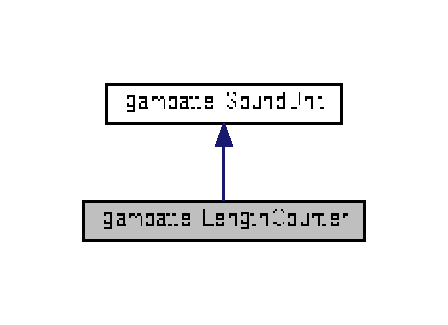
\includegraphics[width=215pt]{classgambatte_1_1LengthCounter__inherit__graph}
\end{center}
\end{figure}


Collaboration diagram for gambatte\+:\+:Length\+Counter\+:
\nopagebreak
\begin{figure}[H]
\begin{center}
\leavevmode
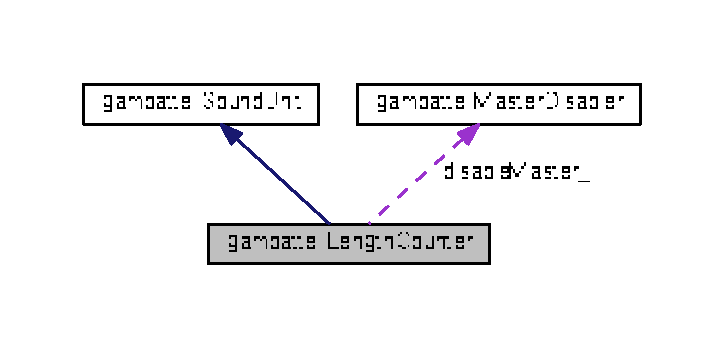
\includegraphics[width=348pt]{classgambatte_1_1LengthCounter__coll__graph}
\end{center}
\end{figure}
\subsection*{Public Member Functions}
\begin{DoxyCompactItemize}
\item 
\hyperlink{classgambatte_1_1LengthCounter_aa654f8aecadd8f7f6c1896cc0fa23592}{Length\+Counter} (\hyperlink{classgambatte_1_1MasterDisabler}{Master\+Disabler} \&disabler, unsigned length\+Mask)
\item 
void \hyperlink{classgambatte_1_1LengthCounter_ad766b7f12bd30af4222cc9da435982b4}{load\+Or\+Save} (\hyperlink{classgambatte_1_1loadsave}{loadsave} \&\hyperlink{ppu_8cpp_a2f2eca6997ee7baf8901725ae074d45b}{state})
\item 
virtual void \hyperlink{classgambatte_1_1LengthCounter_ab0d3eda374d487f8a0b79ea447cca91a}{event} ()
\item 
void \hyperlink{classgambatte_1_1LengthCounter_a6b639f057dab0919908784e350b80228}{nr1\+Change} (unsigned new\+Nr1, unsigned nr4, unsigned cc)
\item 
void \hyperlink{classgambatte_1_1LengthCounter_a30e1eb09f738c51a75fa5ddd8bf41457}{nr4\+Change} (unsigned old\+Nr4, unsigned new\+Nr4, unsigned cc)
\item 
void \hyperlink{classgambatte_1_1LengthCounter_aa04df35be4639e81df42171dce3d1934}{init} (bool cgb)
\item 
void \hyperlink{classgambatte_1_1LengthCounter_a161626ce1c41fe0dc53dfdb40f5644ce}{save\+State} (\hyperlink{structgambatte_1_1SaveState_1_1SPU_1_1LCounter}{Save\+State\+::\+S\+P\+U\+::\+L\+Counter} \&lstate) const
\item 
void \hyperlink{classgambatte_1_1LengthCounter_ae49c50bda45d0d4056f31a3968294930}{load\+State} (\hyperlink{structgambatte_1_1SaveState_1_1SPU_1_1LCounter}{Save\+State\+::\+S\+P\+U\+::\+L\+Counter} const \&lstate, unsigned cc)
\end{DoxyCompactItemize}
\subsection*{Private Attributes}
\begin{DoxyCompactItemize}
\item 
\hyperlink{classgambatte_1_1MasterDisabler}{Master\+Disabler} \& \hyperlink{classgambatte_1_1LengthCounter_acad0b5c512a481252e37952e6a98888b}{disable\+Master\+\_\+}
\item 
unsigned short \hyperlink{classgambatte_1_1LengthCounter_abe18ec36f5b6989a094f681b7fb43a10}{length\+Counter\+\_\+}
\item 
unsigned char const \hyperlink{classgambatte_1_1LengthCounter_a48c36b01e764cde4ff589c1618422475}{length\+Mask\+\_\+}
\item 
bool \hyperlink{classgambatte_1_1LengthCounter_af5baee85c0c722bc5a192f1200969f70}{cgb\+\_\+}
\end{DoxyCompactItemize}
\subsection*{Additional Inherited Members}


\subsection{Constructor \& Destructor Documentation}
\mbox{\Hypertarget{classgambatte_1_1LengthCounter_aa654f8aecadd8f7f6c1896cc0fa23592}\label{classgambatte_1_1LengthCounter_aa654f8aecadd8f7f6c1896cc0fa23592}} 
\index{gambatte\+::\+Length\+Counter@{gambatte\+::\+Length\+Counter}!Length\+Counter@{Length\+Counter}}
\index{Length\+Counter@{Length\+Counter}!gambatte\+::\+Length\+Counter@{gambatte\+::\+Length\+Counter}}
\subsubsection{\texorpdfstring{Length\+Counter()}{LengthCounter()}}
{\footnotesize\ttfamily gambatte\+::\+Length\+Counter\+::\+Length\+Counter (\begin{DoxyParamCaption}\item[{\hyperlink{classgambatte_1_1MasterDisabler}{Master\+Disabler} \&}]{disabler,  }\item[{unsigned}]{length\+Mask }\end{DoxyParamCaption})}



\subsection{Member Function Documentation}
\mbox{\Hypertarget{classgambatte_1_1LengthCounter_ab0d3eda374d487f8a0b79ea447cca91a}\label{classgambatte_1_1LengthCounter_ab0d3eda374d487f8a0b79ea447cca91a}} 
\index{gambatte\+::\+Length\+Counter@{gambatte\+::\+Length\+Counter}!event@{event}}
\index{event@{event}!gambatte\+::\+Length\+Counter@{gambatte\+::\+Length\+Counter}}
\subsubsection{\texorpdfstring{event()}{event()}}
{\footnotesize\ttfamily void gambatte\+::\+Length\+Counter\+::event (\begin{DoxyParamCaption}{ }\end{DoxyParamCaption})\hspace{0.3cm}{\ttfamily [virtual]}}



Implements \hyperlink{classgambatte_1_1SoundUnit_a8ad6df87fc3700d9d3bee470383197b4}{gambatte\+::\+Sound\+Unit}.

\mbox{\Hypertarget{classgambatte_1_1LengthCounter_aa04df35be4639e81df42171dce3d1934}\label{classgambatte_1_1LengthCounter_aa04df35be4639e81df42171dce3d1934}} 
\index{gambatte\+::\+Length\+Counter@{gambatte\+::\+Length\+Counter}!init@{init}}
\index{init@{init}!gambatte\+::\+Length\+Counter@{gambatte\+::\+Length\+Counter}}
\subsubsection{\texorpdfstring{init()}{init()}}
{\footnotesize\ttfamily void gambatte\+::\+Length\+Counter\+::init (\begin{DoxyParamCaption}\item[{bool}]{cgb }\end{DoxyParamCaption})}

\mbox{\Hypertarget{classgambatte_1_1LengthCounter_ad766b7f12bd30af4222cc9da435982b4}\label{classgambatte_1_1LengthCounter_ad766b7f12bd30af4222cc9da435982b4}} 
\index{gambatte\+::\+Length\+Counter@{gambatte\+::\+Length\+Counter}!load\+Or\+Save@{load\+Or\+Save}}
\index{load\+Or\+Save@{load\+Or\+Save}!gambatte\+::\+Length\+Counter@{gambatte\+::\+Length\+Counter}}
\subsubsection{\texorpdfstring{load\+Or\+Save()}{loadOrSave()}}
{\footnotesize\ttfamily void gambatte\+::\+Length\+Counter\+::load\+Or\+Save (\begin{DoxyParamCaption}\item[{\hyperlink{classgambatte_1_1loadsave}{loadsave} \&}]{state }\end{DoxyParamCaption})}

\mbox{\Hypertarget{classgambatte_1_1LengthCounter_ae49c50bda45d0d4056f31a3968294930}\label{classgambatte_1_1LengthCounter_ae49c50bda45d0d4056f31a3968294930}} 
\index{gambatte\+::\+Length\+Counter@{gambatte\+::\+Length\+Counter}!load\+State@{load\+State}}
\index{load\+State@{load\+State}!gambatte\+::\+Length\+Counter@{gambatte\+::\+Length\+Counter}}
\subsubsection{\texorpdfstring{load\+State()}{loadState()}}
{\footnotesize\ttfamily void gambatte\+::\+Length\+Counter\+::load\+State (\begin{DoxyParamCaption}\item[{\hyperlink{structgambatte_1_1SaveState_1_1SPU_1_1LCounter}{Save\+State\+::\+S\+P\+U\+::\+L\+Counter} const \&}]{lstate,  }\item[{unsigned}]{cc }\end{DoxyParamCaption})}

\mbox{\Hypertarget{classgambatte_1_1LengthCounter_a6b639f057dab0919908784e350b80228}\label{classgambatte_1_1LengthCounter_a6b639f057dab0919908784e350b80228}} 
\index{gambatte\+::\+Length\+Counter@{gambatte\+::\+Length\+Counter}!nr1\+Change@{nr1\+Change}}
\index{nr1\+Change@{nr1\+Change}!gambatte\+::\+Length\+Counter@{gambatte\+::\+Length\+Counter}}
\subsubsection{\texorpdfstring{nr1\+Change()}{nr1Change()}}
{\footnotesize\ttfamily void gambatte\+::\+Length\+Counter\+::nr1\+Change (\begin{DoxyParamCaption}\item[{unsigned}]{new\+Nr1,  }\item[{unsigned}]{nr4,  }\item[{unsigned}]{cc }\end{DoxyParamCaption})}

\mbox{\Hypertarget{classgambatte_1_1LengthCounter_a30e1eb09f738c51a75fa5ddd8bf41457}\label{classgambatte_1_1LengthCounter_a30e1eb09f738c51a75fa5ddd8bf41457}} 
\index{gambatte\+::\+Length\+Counter@{gambatte\+::\+Length\+Counter}!nr4\+Change@{nr4\+Change}}
\index{nr4\+Change@{nr4\+Change}!gambatte\+::\+Length\+Counter@{gambatte\+::\+Length\+Counter}}
\subsubsection{\texorpdfstring{nr4\+Change()}{nr4Change()}}
{\footnotesize\ttfamily void gambatte\+::\+Length\+Counter\+::nr4\+Change (\begin{DoxyParamCaption}\item[{unsigned}]{old\+Nr4,  }\item[{unsigned}]{new\+Nr4,  }\item[{unsigned}]{cc }\end{DoxyParamCaption})}

\mbox{\Hypertarget{classgambatte_1_1LengthCounter_a161626ce1c41fe0dc53dfdb40f5644ce}\label{classgambatte_1_1LengthCounter_a161626ce1c41fe0dc53dfdb40f5644ce}} 
\index{gambatte\+::\+Length\+Counter@{gambatte\+::\+Length\+Counter}!save\+State@{save\+State}}
\index{save\+State@{save\+State}!gambatte\+::\+Length\+Counter@{gambatte\+::\+Length\+Counter}}
\subsubsection{\texorpdfstring{save\+State()}{saveState()}}
{\footnotesize\ttfamily void gambatte\+::\+Length\+Counter\+::save\+State (\begin{DoxyParamCaption}\item[{\hyperlink{structgambatte_1_1SaveState_1_1SPU_1_1LCounter}{Save\+State\+::\+S\+P\+U\+::\+L\+Counter} \&}]{lstate }\end{DoxyParamCaption}) const}



\subsection{Member Data Documentation}
\mbox{\Hypertarget{classgambatte_1_1LengthCounter_af5baee85c0c722bc5a192f1200969f70}\label{classgambatte_1_1LengthCounter_af5baee85c0c722bc5a192f1200969f70}} 
\index{gambatte\+::\+Length\+Counter@{gambatte\+::\+Length\+Counter}!cgb\+\_\+@{cgb\+\_\+}}
\index{cgb\+\_\+@{cgb\+\_\+}!gambatte\+::\+Length\+Counter@{gambatte\+::\+Length\+Counter}}
\subsubsection{\texorpdfstring{cgb\+\_\+}{cgb\_}}
{\footnotesize\ttfamily bool gambatte\+::\+Length\+Counter\+::cgb\+\_\+\hspace{0.3cm}{\ttfamily [private]}}

\mbox{\Hypertarget{classgambatte_1_1LengthCounter_acad0b5c512a481252e37952e6a98888b}\label{classgambatte_1_1LengthCounter_acad0b5c512a481252e37952e6a98888b}} 
\index{gambatte\+::\+Length\+Counter@{gambatte\+::\+Length\+Counter}!disable\+Master\+\_\+@{disable\+Master\+\_\+}}
\index{disable\+Master\+\_\+@{disable\+Master\+\_\+}!gambatte\+::\+Length\+Counter@{gambatte\+::\+Length\+Counter}}
\subsubsection{\texorpdfstring{disable\+Master\+\_\+}{disableMaster\_}}
{\footnotesize\ttfamily \hyperlink{classgambatte_1_1MasterDisabler}{Master\+Disabler}\& gambatte\+::\+Length\+Counter\+::disable\+Master\+\_\+\hspace{0.3cm}{\ttfamily [private]}}

\mbox{\Hypertarget{classgambatte_1_1LengthCounter_abe18ec36f5b6989a094f681b7fb43a10}\label{classgambatte_1_1LengthCounter_abe18ec36f5b6989a094f681b7fb43a10}} 
\index{gambatte\+::\+Length\+Counter@{gambatte\+::\+Length\+Counter}!length\+Counter\+\_\+@{length\+Counter\+\_\+}}
\index{length\+Counter\+\_\+@{length\+Counter\+\_\+}!gambatte\+::\+Length\+Counter@{gambatte\+::\+Length\+Counter}}
\subsubsection{\texorpdfstring{length\+Counter\+\_\+}{lengthCounter\_}}
{\footnotesize\ttfamily unsigned short gambatte\+::\+Length\+Counter\+::length\+Counter\+\_\+\hspace{0.3cm}{\ttfamily [private]}}

\mbox{\Hypertarget{classgambatte_1_1LengthCounter_a48c36b01e764cde4ff589c1618422475}\label{classgambatte_1_1LengthCounter_a48c36b01e764cde4ff589c1618422475}} 
\index{gambatte\+::\+Length\+Counter@{gambatte\+::\+Length\+Counter}!length\+Mask\+\_\+@{length\+Mask\+\_\+}}
\index{length\+Mask\+\_\+@{length\+Mask\+\_\+}!gambatte\+::\+Length\+Counter@{gambatte\+::\+Length\+Counter}}
\subsubsection{\texorpdfstring{length\+Mask\+\_\+}{lengthMask\_}}
{\footnotesize\ttfamily unsigned char const gambatte\+::\+Length\+Counter\+::length\+Mask\+\_\+\hspace{0.3cm}{\ttfamily [private]}}



The documentation for this class was generated from the following files\+:\begin{DoxyCompactItemize}
\item 
src/sound/\hyperlink{length__counter_8h}{length\+\_\+counter.\+h}\item 
src/sound/\hyperlink{length__counter_8cpp}{length\+\_\+counter.\+cpp}\end{DoxyCompactItemize}

\hypertarget{classgambatte_1_1Channel4_1_1Lfsr}{}\section{gambatte\+:\+:Channel4\+:\+:Lfsr Class Reference}
\label{classgambatte_1_1Channel4_1_1Lfsr}\index{gambatte\+::\+Channel4\+::\+Lfsr@{gambatte\+::\+Channel4\+::\+Lfsr}}


Inheritance diagram for gambatte\+:\+:Channel4\+:\+:Lfsr\+:
\nopagebreak
\begin{figure}[H]
\begin{center}
\leavevmode
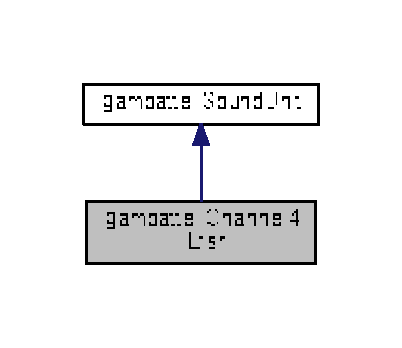
\includegraphics[width=193pt]{classgambatte_1_1Channel4_1_1Lfsr__inherit__graph}
\end{center}
\end{figure}


Collaboration diagram for gambatte\+:\+:Channel4\+:\+:Lfsr\+:
\nopagebreak
\begin{figure}[H]
\begin{center}
\leavevmode
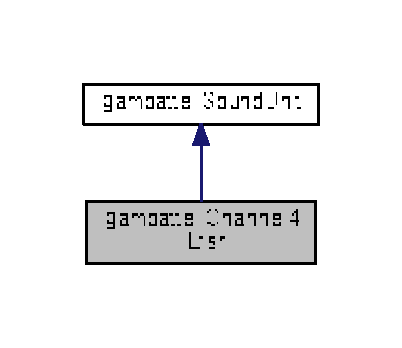
\includegraphics[width=193pt]{classgambatte_1_1Channel4_1_1Lfsr__coll__graph}
\end{center}
\end{figure}
\subsection*{Public Member Functions}
\begin{DoxyCompactItemize}
\item 
\hyperlink{classgambatte_1_1Channel4_1_1Lfsr_a070b6af35c8738378554108722c117ae}{Lfsr} ()
\item 
virtual void \hyperlink{classgambatte_1_1Channel4_1_1Lfsr_a019ab6fad6c598fdc6f061b70df93fdc}{event} ()
\item 
void \hyperlink{classgambatte_1_1Channel4_1_1Lfsr_a7efc0bc0a1075903d2228997d5ecfafa}{load\+Or\+Save} (\hyperlink{classgambatte_1_1loadsave}{loadsave} \&\hyperlink{ppu_8cpp_a2f2eca6997ee7baf8901725ae074d45b}{state})
\item 
virtual void \hyperlink{classgambatte_1_1Channel4_1_1Lfsr_acdeb93a45132b45567f97878ed6306b9}{reset\+Counters} (unsigned old\+Cc)
\item 
bool \hyperlink{classgambatte_1_1Channel4_1_1Lfsr_ac711ac75e9618a2a00305909dd1f380e}{is\+High\+State} () const
\item 
void \hyperlink{classgambatte_1_1Channel4_1_1Lfsr_a2247d65d109fdcf2f284cbb1c22ec839}{nr3\+Change} (unsigned new\+Nr3, unsigned cc)
\item 
void \hyperlink{classgambatte_1_1Channel4_1_1Lfsr_addb216b88720928bdf43b93366dd187d}{nr4\+Init} (unsigned cc)
\item 
void \hyperlink{classgambatte_1_1Channel4_1_1Lfsr_a8a7f22b16436748c37b64fca7c4e7774}{reset} (unsigned cc)
\item 
void \hyperlink{classgambatte_1_1Channel4_1_1Lfsr_ab3f65da97d38ed85258dbe58fe282d4f}{save\+State} (\hyperlink{structgambatte_1_1SaveState}{Save\+State} \&\hyperlink{ppu_8cpp_a2f2eca6997ee7baf8901725ae074d45b}{state}, unsigned cc)
\item 
void \hyperlink{classgambatte_1_1Channel4_1_1Lfsr_a7600ceb0f1867552977cfcc5fd07e39b}{load\+State} (\hyperlink{structgambatte_1_1SaveState}{Save\+State} const \&\hyperlink{ppu_8cpp_a2f2eca6997ee7baf8901725ae074d45b}{state})
\item 
void \hyperlink{classgambatte_1_1Channel4_1_1Lfsr_a9853ba5c6b10344cea14208f3c5a5558}{disable\+Master} ()
\item 
void \hyperlink{classgambatte_1_1Channel4_1_1Lfsr_a2ed2547ea57bf2ecf592345c8066419d}{kill\+Counter} ()
\item 
void \hyperlink{classgambatte_1_1Channel4_1_1Lfsr_a6cbac4af17a2cb4cc35ef46d850ed2dd}{revive\+Counter} (unsigned cc)
\end{DoxyCompactItemize}
\subsection*{Private Member Functions}
\begin{DoxyCompactItemize}
\item 
void \hyperlink{classgambatte_1_1Channel4_1_1Lfsr_a1a123ac84edbac35f1d63be538afa0aa}{update\+Backup\+Counter} (unsigned cc)
\end{DoxyCompactItemize}
\subsection*{Private Attributes}
\begin{DoxyCompactItemize}
\item 
unsigned \hyperlink{classgambatte_1_1Channel4_1_1Lfsr_aa87d60c609b2fdf21e1344430e4f8098}{backup\+Counter\+\_\+}
\item 
unsigned short \hyperlink{classgambatte_1_1Channel4_1_1Lfsr_a1c1805ef084771b4cc2e9905d35f93b9}{reg\+\_\+}
\item 
unsigned char \hyperlink{classgambatte_1_1Channel4_1_1Lfsr_a831fdbeb316609dc1e4c78f11891a2bb}{nr3\+\_\+}
\item 
bool \hyperlink{classgambatte_1_1Channel4_1_1Lfsr_a93cd98bd46a36129edf01ea052358c8b}{master\+\_\+}
\end{DoxyCompactItemize}
\subsection*{Additional Inherited Members}


\subsection{Constructor \& Destructor Documentation}
\mbox{\Hypertarget{classgambatte_1_1Channel4_1_1Lfsr_a070b6af35c8738378554108722c117ae}\label{classgambatte_1_1Channel4_1_1Lfsr_a070b6af35c8738378554108722c117ae}} 
\index{gambatte\+::\+Channel4\+::\+Lfsr@{gambatte\+::\+Channel4\+::\+Lfsr}!Lfsr@{Lfsr}}
\index{Lfsr@{Lfsr}!gambatte\+::\+Channel4\+::\+Lfsr@{gambatte\+::\+Channel4\+::\+Lfsr}}
\subsubsection{\texorpdfstring{Lfsr()}{Lfsr()}}
{\footnotesize\ttfamily gambatte\+::\+Channel4\+::\+Lfsr\+::\+Lfsr (\begin{DoxyParamCaption}{ }\end{DoxyParamCaption})}



\subsection{Member Function Documentation}
\mbox{\Hypertarget{classgambatte_1_1Channel4_1_1Lfsr_a9853ba5c6b10344cea14208f3c5a5558}\label{classgambatte_1_1Channel4_1_1Lfsr_a9853ba5c6b10344cea14208f3c5a5558}} 
\index{gambatte\+::\+Channel4\+::\+Lfsr@{gambatte\+::\+Channel4\+::\+Lfsr}!disable\+Master@{disable\+Master}}
\index{disable\+Master@{disable\+Master}!gambatte\+::\+Channel4\+::\+Lfsr@{gambatte\+::\+Channel4\+::\+Lfsr}}
\subsubsection{\texorpdfstring{disable\+Master()}{disableMaster()}}
{\footnotesize\ttfamily void gambatte\+::\+Channel4\+::\+Lfsr\+::disable\+Master (\begin{DoxyParamCaption}{ }\end{DoxyParamCaption})\hspace{0.3cm}{\ttfamily [inline]}}

\mbox{\Hypertarget{classgambatte_1_1Channel4_1_1Lfsr_a019ab6fad6c598fdc6f061b70df93fdc}\label{classgambatte_1_1Channel4_1_1Lfsr_a019ab6fad6c598fdc6f061b70df93fdc}} 
\index{gambatte\+::\+Channel4\+::\+Lfsr@{gambatte\+::\+Channel4\+::\+Lfsr}!event@{event}}
\index{event@{event}!gambatte\+::\+Channel4\+::\+Lfsr@{gambatte\+::\+Channel4\+::\+Lfsr}}
\subsubsection{\texorpdfstring{event()}{event()}}
{\footnotesize\ttfamily void gambatte\+::\+Channel4\+::\+Lfsr\+::event (\begin{DoxyParamCaption}{ }\end{DoxyParamCaption})\hspace{0.3cm}{\ttfamily [inline]}, {\ttfamily [virtual]}}



Implements \hyperlink{classgambatte_1_1SoundUnit_a8ad6df87fc3700d9d3bee470383197b4}{gambatte\+::\+Sound\+Unit}.

\mbox{\Hypertarget{classgambatte_1_1Channel4_1_1Lfsr_ac711ac75e9618a2a00305909dd1f380e}\label{classgambatte_1_1Channel4_1_1Lfsr_ac711ac75e9618a2a00305909dd1f380e}} 
\index{gambatte\+::\+Channel4\+::\+Lfsr@{gambatte\+::\+Channel4\+::\+Lfsr}!is\+High\+State@{is\+High\+State}}
\index{is\+High\+State@{is\+High\+State}!gambatte\+::\+Channel4\+::\+Lfsr@{gambatte\+::\+Channel4\+::\+Lfsr}}
\subsubsection{\texorpdfstring{is\+High\+State()}{isHighState()}}
{\footnotesize\ttfamily bool gambatte\+::\+Channel4\+::\+Lfsr\+::is\+High\+State (\begin{DoxyParamCaption}{ }\end{DoxyParamCaption}) const\hspace{0.3cm}{\ttfamily [inline]}}

\mbox{\Hypertarget{classgambatte_1_1Channel4_1_1Lfsr_a2ed2547ea57bf2ecf592345c8066419d}\label{classgambatte_1_1Channel4_1_1Lfsr_a2ed2547ea57bf2ecf592345c8066419d}} 
\index{gambatte\+::\+Channel4\+::\+Lfsr@{gambatte\+::\+Channel4\+::\+Lfsr}!kill\+Counter@{kill\+Counter}}
\index{kill\+Counter@{kill\+Counter}!gambatte\+::\+Channel4\+::\+Lfsr@{gambatte\+::\+Channel4\+::\+Lfsr}}
\subsubsection{\texorpdfstring{kill\+Counter()}{killCounter()}}
{\footnotesize\ttfamily void gambatte\+::\+Channel4\+::\+Lfsr\+::kill\+Counter (\begin{DoxyParamCaption}{ }\end{DoxyParamCaption})\hspace{0.3cm}{\ttfamily [inline]}}

\mbox{\Hypertarget{classgambatte_1_1Channel4_1_1Lfsr_a7efc0bc0a1075903d2228997d5ecfafa}\label{classgambatte_1_1Channel4_1_1Lfsr_a7efc0bc0a1075903d2228997d5ecfafa}} 
\index{gambatte\+::\+Channel4\+::\+Lfsr@{gambatte\+::\+Channel4\+::\+Lfsr}!load\+Or\+Save@{load\+Or\+Save}}
\index{load\+Or\+Save@{load\+Or\+Save}!gambatte\+::\+Channel4\+::\+Lfsr@{gambatte\+::\+Channel4\+::\+Lfsr}}
\subsubsection{\texorpdfstring{load\+Or\+Save()}{loadOrSave()}}
{\footnotesize\ttfamily void gambatte\+::\+Channel4\+::\+Lfsr\+::load\+Or\+Save (\begin{DoxyParamCaption}\item[{\hyperlink{classgambatte_1_1loadsave}{loadsave} \&}]{state }\end{DoxyParamCaption})\hspace{0.3cm}{\ttfamily [inline]}}

\mbox{\Hypertarget{classgambatte_1_1Channel4_1_1Lfsr_a7600ceb0f1867552977cfcc5fd07e39b}\label{classgambatte_1_1Channel4_1_1Lfsr_a7600ceb0f1867552977cfcc5fd07e39b}} 
\index{gambatte\+::\+Channel4\+::\+Lfsr@{gambatte\+::\+Channel4\+::\+Lfsr}!load\+State@{load\+State}}
\index{load\+State@{load\+State}!gambatte\+::\+Channel4\+::\+Lfsr@{gambatte\+::\+Channel4\+::\+Lfsr}}
\subsubsection{\texorpdfstring{load\+State()}{loadState()}}
{\footnotesize\ttfamily void gambatte\+::\+Channel4\+::\+Lfsr\+::load\+State (\begin{DoxyParamCaption}\item[{\hyperlink{structgambatte_1_1SaveState}{Save\+State} const \&}]{state }\end{DoxyParamCaption})}

\mbox{\Hypertarget{classgambatte_1_1Channel4_1_1Lfsr_a2247d65d109fdcf2f284cbb1c22ec839}\label{classgambatte_1_1Channel4_1_1Lfsr_a2247d65d109fdcf2f284cbb1c22ec839}} 
\index{gambatte\+::\+Channel4\+::\+Lfsr@{gambatte\+::\+Channel4\+::\+Lfsr}!nr3\+Change@{nr3\+Change}}
\index{nr3\+Change@{nr3\+Change}!gambatte\+::\+Channel4\+::\+Lfsr@{gambatte\+::\+Channel4\+::\+Lfsr}}
\subsubsection{\texorpdfstring{nr3\+Change()}{nr3Change()}}
{\footnotesize\ttfamily void gambatte\+::\+Channel4\+::\+Lfsr\+::nr3\+Change (\begin{DoxyParamCaption}\item[{unsigned}]{new\+Nr3,  }\item[{unsigned}]{cc }\end{DoxyParamCaption})}

\mbox{\Hypertarget{classgambatte_1_1Channel4_1_1Lfsr_addb216b88720928bdf43b93366dd187d}\label{classgambatte_1_1Channel4_1_1Lfsr_addb216b88720928bdf43b93366dd187d}} 
\index{gambatte\+::\+Channel4\+::\+Lfsr@{gambatte\+::\+Channel4\+::\+Lfsr}!nr4\+Init@{nr4\+Init}}
\index{nr4\+Init@{nr4\+Init}!gambatte\+::\+Channel4\+::\+Lfsr@{gambatte\+::\+Channel4\+::\+Lfsr}}
\subsubsection{\texorpdfstring{nr4\+Init()}{nr4Init()}}
{\footnotesize\ttfamily void gambatte\+::\+Channel4\+::\+Lfsr\+::nr4\+Init (\begin{DoxyParamCaption}\item[{unsigned}]{cc }\end{DoxyParamCaption})}

\mbox{\Hypertarget{classgambatte_1_1Channel4_1_1Lfsr_a8a7f22b16436748c37b64fca7c4e7774}\label{classgambatte_1_1Channel4_1_1Lfsr_a8a7f22b16436748c37b64fca7c4e7774}} 
\index{gambatte\+::\+Channel4\+::\+Lfsr@{gambatte\+::\+Channel4\+::\+Lfsr}!reset@{reset}}
\index{reset@{reset}!gambatte\+::\+Channel4\+::\+Lfsr@{gambatte\+::\+Channel4\+::\+Lfsr}}
\subsubsection{\texorpdfstring{reset()}{reset()}}
{\footnotesize\ttfamily void gambatte\+::\+Channel4\+::\+Lfsr\+::reset (\begin{DoxyParamCaption}\item[{unsigned}]{cc }\end{DoxyParamCaption})}

\mbox{\Hypertarget{classgambatte_1_1Channel4_1_1Lfsr_acdeb93a45132b45567f97878ed6306b9}\label{classgambatte_1_1Channel4_1_1Lfsr_acdeb93a45132b45567f97878ed6306b9}} 
\index{gambatte\+::\+Channel4\+::\+Lfsr@{gambatte\+::\+Channel4\+::\+Lfsr}!reset\+Counters@{reset\+Counters}}
\index{reset\+Counters@{reset\+Counters}!gambatte\+::\+Channel4\+::\+Lfsr@{gambatte\+::\+Channel4\+::\+Lfsr}}
\subsubsection{\texorpdfstring{reset\+Counters()}{resetCounters()}}
{\footnotesize\ttfamily void gambatte\+::\+Channel4\+::\+Lfsr\+::reset\+Counters (\begin{DoxyParamCaption}\item[{unsigned}]{old\+Cc }\end{DoxyParamCaption})\hspace{0.3cm}{\ttfamily [virtual]}}



Reimplemented from \hyperlink{classgambatte_1_1SoundUnit_a3baa270f75463b24cd79fe5970103d4f}{gambatte\+::\+Sound\+Unit}.

\mbox{\Hypertarget{classgambatte_1_1Channel4_1_1Lfsr_a6cbac4af17a2cb4cc35ef46d850ed2dd}\label{classgambatte_1_1Channel4_1_1Lfsr_a6cbac4af17a2cb4cc35ef46d850ed2dd}} 
\index{gambatte\+::\+Channel4\+::\+Lfsr@{gambatte\+::\+Channel4\+::\+Lfsr}!revive\+Counter@{revive\+Counter}}
\index{revive\+Counter@{revive\+Counter}!gambatte\+::\+Channel4\+::\+Lfsr@{gambatte\+::\+Channel4\+::\+Lfsr}}
\subsubsection{\texorpdfstring{revive\+Counter()}{reviveCounter()}}
{\footnotesize\ttfamily void gambatte\+::\+Channel4\+::\+Lfsr\+::revive\+Counter (\begin{DoxyParamCaption}\item[{unsigned}]{cc }\end{DoxyParamCaption})}

\mbox{\Hypertarget{classgambatte_1_1Channel4_1_1Lfsr_ab3f65da97d38ed85258dbe58fe282d4f}\label{classgambatte_1_1Channel4_1_1Lfsr_ab3f65da97d38ed85258dbe58fe282d4f}} 
\index{gambatte\+::\+Channel4\+::\+Lfsr@{gambatte\+::\+Channel4\+::\+Lfsr}!save\+State@{save\+State}}
\index{save\+State@{save\+State}!gambatte\+::\+Channel4\+::\+Lfsr@{gambatte\+::\+Channel4\+::\+Lfsr}}
\subsubsection{\texorpdfstring{save\+State()}{saveState()}}
{\footnotesize\ttfamily void gambatte\+::\+Channel4\+::\+Lfsr\+::save\+State (\begin{DoxyParamCaption}\item[{\hyperlink{structgambatte_1_1SaveState}{Save\+State} \&}]{state,  }\item[{unsigned}]{cc }\end{DoxyParamCaption})}

\mbox{\Hypertarget{classgambatte_1_1Channel4_1_1Lfsr_a1a123ac84edbac35f1d63be538afa0aa}\label{classgambatte_1_1Channel4_1_1Lfsr_a1a123ac84edbac35f1d63be538afa0aa}} 
\index{gambatte\+::\+Channel4\+::\+Lfsr@{gambatte\+::\+Channel4\+::\+Lfsr}!update\+Backup\+Counter@{update\+Backup\+Counter}}
\index{update\+Backup\+Counter@{update\+Backup\+Counter}!gambatte\+::\+Channel4\+::\+Lfsr@{gambatte\+::\+Channel4\+::\+Lfsr}}
\subsubsection{\texorpdfstring{update\+Backup\+Counter()}{updateBackupCounter()}}
{\footnotesize\ttfamily void gambatte\+::\+Channel4\+::\+Lfsr\+::update\+Backup\+Counter (\begin{DoxyParamCaption}\item[{unsigned}]{cc }\end{DoxyParamCaption})\hspace{0.3cm}{\ttfamily [private]}}



\subsection{Member Data Documentation}
\mbox{\Hypertarget{classgambatte_1_1Channel4_1_1Lfsr_aa87d60c609b2fdf21e1344430e4f8098}\label{classgambatte_1_1Channel4_1_1Lfsr_aa87d60c609b2fdf21e1344430e4f8098}} 
\index{gambatte\+::\+Channel4\+::\+Lfsr@{gambatte\+::\+Channel4\+::\+Lfsr}!backup\+Counter\+\_\+@{backup\+Counter\+\_\+}}
\index{backup\+Counter\+\_\+@{backup\+Counter\+\_\+}!gambatte\+::\+Channel4\+::\+Lfsr@{gambatte\+::\+Channel4\+::\+Lfsr}}
\subsubsection{\texorpdfstring{backup\+Counter\+\_\+}{backupCounter\_}}
{\footnotesize\ttfamily unsigned gambatte\+::\+Channel4\+::\+Lfsr\+::backup\+Counter\+\_\+\hspace{0.3cm}{\ttfamily [private]}}

\mbox{\Hypertarget{classgambatte_1_1Channel4_1_1Lfsr_a93cd98bd46a36129edf01ea052358c8b}\label{classgambatte_1_1Channel4_1_1Lfsr_a93cd98bd46a36129edf01ea052358c8b}} 
\index{gambatte\+::\+Channel4\+::\+Lfsr@{gambatte\+::\+Channel4\+::\+Lfsr}!master\+\_\+@{master\+\_\+}}
\index{master\+\_\+@{master\+\_\+}!gambatte\+::\+Channel4\+::\+Lfsr@{gambatte\+::\+Channel4\+::\+Lfsr}}
\subsubsection{\texorpdfstring{master\+\_\+}{master\_}}
{\footnotesize\ttfamily bool gambatte\+::\+Channel4\+::\+Lfsr\+::master\+\_\+\hspace{0.3cm}{\ttfamily [private]}}

\mbox{\Hypertarget{classgambatte_1_1Channel4_1_1Lfsr_a831fdbeb316609dc1e4c78f11891a2bb}\label{classgambatte_1_1Channel4_1_1Lfsr_a831fdbeb316609dc1e4c78f11891a2bb}} 
\index{gambatte\+::\+Channel4\+::\+Lfsr@{gambatte\+::\+Channel4\+::\+Lfsr}!nr3\+\_\+@{nr3\+\_\+}}
\index{nr3\+\_\+@{nr3\+\_\+}!gambatte\+::\+Channel4\+::\+Lfsr@{gambatte\+::\+Channel4\+::\+Lfsr}}
\subsubsection{\texorpdfstring{nr3\+\_\+}{nr3\_}}
{\footnotesize\ttfamily unsigned char gambatte\+::\+Channel4\+::\+Lfsr\+::nr3\+\_\+\hspace{0.3cm}{\ttfamily [private]}}

\mbox{\Hypertarget{classgambatte_1_1Channel4_1_1Lfsr_a1c1805ef084771b4cc2e9905d35f93b9}\label{classgambatte_1_1Channel4_1_1Lfsr_a1c1805ef084771b4cc2e9905d35f93b9}} 
\index{gambatte\+::\+Channel4\+::\+Lfsr@{gambatte\+::\+Channel4\+::\+Lfsr}!reg\+\_\+@{reg\+\_\+}}
\index{reg\+\_\+@{reg\+\_\+}!gambatte\+::\+Channel4\+::\+Lfsr@{gambatte\+::\+Channel4\+::\+Lfsr}}
\subsubsection{\texorpdfstring{reg\+\_\+}{reg\_}}
{\footnotesize\ttfamily unsigned short gambatte\+::\+Channel4\+::\+Lfsr\+::reg\+\_\+\hspace{0.3cm}{\ttfamily [private]}}



The documentation for this class was generated from the following files\+:\begin{DoxyCompactItemize}
\item 
src/sound/\hyperlink{channel4_8h}{channel4.\+h}\item 
src/sound/\hyperlink{channel4_8cpp}{channel4.\+cpp}\end{DoxyCompactItemize}

\hypertarget{classgambatte_1_1loadsave}{}\section{gambatte\+:\+:loadsave Class Reference}
\label{classgambatte_1_1loadsave}\index{gambatte\+::loadsave@{gambatte\+::loadsave}}


{\ttfamily \#include $<$loadsave.\+h$>$}



Inheritance diagram for gambatte\+:\+:loadsave\+:\nopagebreak
\begin{figure}[H]
\begin{center}
\leavevmode
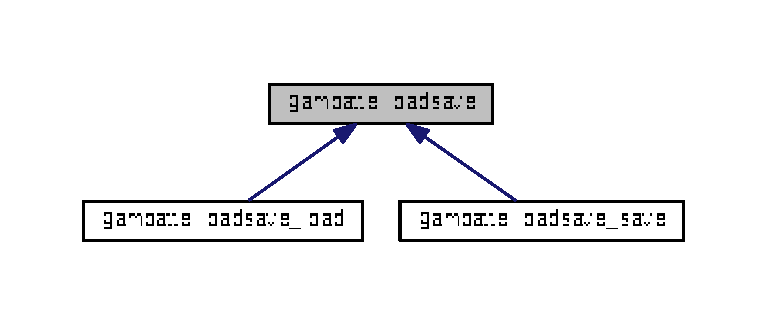
\includegraphics[width=350pt]{classgambatte_1_1loadsave__inherit__graph}
\end{center}
\end{figure}
\subsection*{Public Member Functions}
\begin{DoxyCompactItemize}
\item 
virtual \hyperlink{classgambatte_1_1loadsave_a96a8c63427797752e26a03b4a1c2c495}{$\sim$loadsave} ()  throw ()
\item 
virtual void \hyperlink{classgambatte_1_1loadsave_a286a1bc924db345dda227a735a5ba038}{operator()} (bool \&x)=0
\item 
virtual void \hyperlink{classgambatte_1_1loadsave_abe43ebb74162f066b542781f5ec7e5af}{operator()} (signed char \&x)=0
\item 
virtual void \hyperlink{classgambatte_1_1loadsave_a475286c3cdfc0a207cd6ac9d27bf5b0b}{operator()} (unsigned char \&x)=0
\item 
virtual void \hyperlink{classgambatte_1_1loadsave_a8874e92f76b3765efba593c377667f16}{operator()} (signed short \&x)=0
\item 
virtual void \hyperlink{classgambatte_1_1loadsave_a36c04339183e08d7dbfa0aeabc3c953d}{operator()} (unsigned short \&x)=0
\item 
virtual void \hyperlink{classgambatte_1_1loadsave_a9a8e8765ac066a4d51099147f71595d1}{operator()} (signed \hyperlink{ioapi_8h_a787fa3cf048117ba7123753c1e74fcd6}{int} \&x)=0
\item 
virtual void \hyperlink{classgambatte_1_1loadsave_a263bbb4b470594752ca94548673e66a4}{operator()} (unsigned \hyperlink{ioapi_8h_a787fa3cf048117ba7123753c1e74fcd6}{int} \&x)=0
\item 
virtual void \hyperlink{classgambatte_1_1loadsave_a882deed58830a077498c160ba2870eec}{operator()} (signed \hyperlink{ioapi_8h_a3c7b35ad9dab18b8310343c201f7b27e}{long} \hyperlink{ioapi_8h_a3c7b35ad9dab18b8310343c201f7b27e}{long} \&x)=0
\item 
virtual void \hyperlink{classgambatte_1_1loadsave_aca5dcc05e845b6aa3086065048ab6e29}{operator()} (unsigned \hyperlink{ioapi_8h_a3c7b35ad9dab18b8310343c201f7b27e}{long} \hyperlink{ioapi_8h_a3c7b35ad9dab18b8310343c201f7b27e}{long} \&x)=0
\item 
virtual void \hyperlink{classgambatte_1_1loadsave_a8ba29ce3f56dbaa7ac1d4aec4b705af3}{operator()} (signed char $\ast$x, size\+\_\+t s)=0
\item 
virtual void \hyperlink{classgambatte_1_1loadsave_ae1ab673c435463f83c510446d7455436}{operator()} (unsigned char $\ast$x, size\+\_\+t s)=0
\item 
virtual void \hyperlink{classgambatte_1_1loadsave_ac30751838bea28e3e266da5194b429d1}{operator()} (signed short $\ast$x, size\+\_\+t s)=0
\item 
virtual void \hyperlink{classgambatte_1_1loadsave_aa260c68090c6bb3b5620ac77ce70815d}{operator()} (unsigned short $\ast$x, size\+\_\+t s)=0
\item 
virtual void \hyperlink{classgambatte_1_1loadsave_a9f843edffc4473365246e8620d65f1e3}{operator()} (signed \hyperlink{ioapi_8h_a787fa3cf048117ba7123753c1e74fcd6}{int} $\ast$x, size\+\_\+t s)=0
\item 
virtual void \hyperlink{classgambatte_1_1loadsave_a0985be7f430a1626e2b0f47066e9a8b6}{operator()} (unsigned \hyperlink{ioapi_8h_a787fa3cf048117ba7123753c1e74fcd6}{int} $\ast$x, size\+\_\+t s)=0
\item 
virtual void \hyperlink{classgambatte_1_1loadsave_a34283e091c2bfae20f12f79fff2b8b36}{operator()} (\hyperlink{ioapi_8h_a3c7b35ad9dab18b8310343c201f7b27e}{long} \hyperlink{ioapi_8h_a3c7b35ad9dab18b8310343c201f7b27e}{long} $\ast$x, size\+\_\+t s)=0
\item 
virtual void \hyperlink{classgambatte_1_1loadsave_a93ef67515dbf61461e7370c9cc77c8a6}{operator()} (unsigned \hyperlink{ioapi_8h_a3c7b35ad9dab18b8310343c201f7b27e}{long} \hyperlink{ioapi_8h_a3c7b35ad9dab18b8310343c201f7b27e}{long} $\ast$x, size\+\_\+t s)=0
\item 
virtual void \hyperlink{classgambatte_1_1loadsave_a911a5ce78fbb8c4ceb36984a9967ea72}{operator()} (unsigned char $\ast$\&ptr, unsigned char $\ast$abase)=0
\item 
virtual void \hyperlink{classgambatte_1_1loadsave_a57518c27d7844ae48faea91fc04a680a}{operator()} (const unsigned char $\ast$\&ptr, unsigned char $\ast$abase)=0
\item 
virtual void \hyperlink{classgambatte_1_1loadsave_af4a635fc49c23e53e48b2b9d320aa165}{tag} (unsigned short tag)=0
\item 
void \hyperlink{classgambatte_1_1loadsave_a408680c3fae9e459f3dc4d2e9c6eef04}{time} (time\+\_\+t \&t)
\item 
void \hyperlink{classgambatte_1_1loadsave_acbec8a5cd9098a7a796a863149ed8e22}{start\+Enumeration} ()
\item 
{\footnotesize template$<$typename T $>$ }\\void \hyperlink{classgambatte_1_1loadsave_afead9849579608ea420342ae0ec0feee}{enumerate} (T \&ptr, T candiate, unsigned symbol)
\item 
void \hyperlink{classgambatte_1_1loadsave_a2fd5b7f803fc455d40921d815e07a50d}{end\+Enumeration} ()
\item 
virtual bool \hyperlink{classgambatte_1_1loadsave_a0a05b67eadfbb26f654f3d5ec287c652}{saving} ()=0
\end{DoxyCompactItemize}
\subsection*{Private Attributes}
\begin{DoxyCompactItemize}
\item 
unsigned \hyperlink{classgambatte_1_1loadsave_a4879654f0e5d4751b6ff6797778f3247}{enum\+Val}
\item 
bool \hyperlink{classgambatte_1_1loadsave_a7c680a9fcfcffab3f7cdb137125830f7}{enum\+Assigned}
\end{DoxyCompactItemize}


\subsection{Constructor \& Destructor Documentation}
\mbox{\Hypertarget{classgambatte_1_1loadsave_a96a8c63427797752e26a03b4a1c2c495}\label{classgambatte_1_1loadsave_a96a8c63427797752e26a03b4a1c2c495}} 
\index{gambatte\+::loadsave@{gambatte\+::loadsave}!````~loadsave@{$\sim$loadsave}}
\index{````~loadsave@{$\sim$loadsave}!gambatte\+::loadsave@{gambatte\+::loadsave}}
\subsubsection{\texorpdfstring{$\sim$loadsave()}{~loadsave()}}
{\footnotesize\ttfamily gambatte\+::loadsave\+::$\sim$loadsave (\begin{DoxyParamCaption}{ }\end{DoxyParamCaption}) throw  ) \hspace{0.3cm}{\ttfamily [virtual]}}



\subsection{Member Function Documentation}
\mbox{\Hypertarget{classgambatte_1_1loadsave_a2fd5b7f803fc455d40921d815e07a50d}\label{classgambatte_1_1loadsave_a2fd5b7f803fc455d40921d815e07a50d}} 
\index{gambatte\+::loadsave@{gambatte\+::loadsave}!end\+Enumeration@{end\+Enumeration}}
\index{end\+Enumeration@{end\+Enumeration}!gambatte\+::loadsave@{gambatte\+::loadsave}}
\subsubsection{\texorpdfstring{end\+Enumeration()}{endEnumeration()}}
{\footnotesize\ttfamily void gambatte\+::loadsave\+::end\+Enumeration (\begin{DoxyParamCaption}{ }\end{DoxyParamCaption})\hspace{0.3cm}{\ttfamily [inline]}}

\mbox{\Hypertarget{classgambatte_1_1loadsave_afead9849579608ea420342ae0ec0feee}\label{classgambatte_1_1loadsave_afead9849579608ea420342ae0ec0feee}} 
\index{gambatte\+::loadsave@{gambatte\+::loadsave}!enumerate@{enumerate}}
\index{enumerate@{enumerate}!gambatte\+::loadsave@{gambatte\+::loadsave}}
\subsubsection{\texorpdfstring{enumerate()}{enumerate()}}
{\footnotesize\ttfamily template$<$typename T $>$ \\
void gambatte\+::loadsave\+::enumerate (\begin{DoxyParamCaption}\item[{T \&}]{ptr,  }\item[{T}]{candiate,  }\item[{unsigned}]{symbol }\end{DoxyParamCaption})\hspace{0.3cm}{\ttfamily [inline]}}

\mbox{\Hypertarget{classgambatte_1_1loadsave_a286a1bc924db345dda227a735a5ba038}\label{classgambatte_1_1loadsave_a286a1bc924db345dda227a735a5ba038}} 
\index{gambatte\+::loadsave@{gambatte\+::loadsave}!operator()@{operator()}}
\index{operator()@{operator()}!gambatte\+::loadsave@{gambatte\+::loadsave}}
\subsubsection{\texorpdfstring{operator()()}{operator()()}\hspace{0.1cm}{\footnotesize\ttfamily [1/19]}}
{\footnotesize\ttfamily virtual void gambatte\+::loadsave\+::operator() (\begin{DoxyParamCaption}\item[{bool \&}]{x }\end{DoxyParamCaption})\hspace{0.3cm}{\ttfamily [pure virtual]}}



Implemented in \hyperlink{classgambatte_1_1loadsave__save_a05b06e5e375fede9a5821fc2bbfd1cd9}{gambatte\+::loadsave\+\_\+save}, and \hyperlink{classgambatte_1_1loadsave__load_a551d7c208300ff066c9725c3efff8aa9}{gambatte\+::loadsave\+\_\+load}.

\mbox{\Hypertarget{classgambatte_1_1loadsave_abe43ebb74162f066b542781f5ec7e5af}\label{classgambatte_1_1loadsave_abe43ebb74162f066b542781f5ec7e5af}} 
\index{gambatte\+::loadsave@{gambatte\+::loadsave}!operator()@{operator()}}
\index{operator()@{operator()}!gambatte\+::loadsave@{gambatte\+::loadsave}}
\subsubsection{\texorpdfstring{operator()()}{operator()()}\hspace{0.1cm}{\footnotesize\ttfamily [2/19]}}
{\footnotesize\ttfamily virtual void gambatte\+::loadsave\+::operator() (\begin{DoxyParamCaption}\item[{signed char \&}]{x }\end{DoxyParamCaption})\hspace{0.3cm}{\ttfamily [pure virtual]}}



Implemented in \hyperlink{classgambatte_1_1loadsave__save_a9e8ce089bd78f68b0319105a9a630e38}{gambatte\+::loadsave\+\_\+save}, and \hyperlink{classgambatte_1_1loadsave__load_ae0135e997f4fac56481edb91a3b4e6c0}{gambatte\+::loadsave\+\_\+load}.

\mbox{\Hypertarget{classgambatte_1_1loadsave_a475286c3cdfc0a207cd6ac9d27bf5b0b}\label{classgambatte_1_1loadsave_a475286c3cdfc0a207cd6ac9d27bf5b0b}} 
\index{gambatte\+::loadsave@{gambatte\+::loadsave}!operator()@{operator()}}
\index{operator()@{operator()}!gambatte\+::loadsave@{gambatte\+::loadsave}}
\subsubsection{\texorpdfstring{operator()()}{operator()()}\hspace{0.1cm}{\footnotesize\ttfamily [3/19]}}
{\footnotesize\ttfamily virtual void gambatte\+::loadsave\+::operator() (\begin{DoxyParamCaption}\item[{unsigned char \&}]{x }\end{DoxyParamCaption})\hspace{0.3cm}{\ttfamily [pure virtual]}}



Implemented in \hyperlink{classgambatte_1_1loadsave__save_a5738bf9ee07da4c9c6af989f22e5ba29}{gambatte\+::loadsave\+\_\+save}, and \hyperlink{classgambatte_1_1loadsave__load_a1e6642fca66ae4b43af93815c69d5aba}{gambatte\+::loadsave\+\_\+load}.

\mbox{\Hypertarget{classgambatte_1_1loadsave_a8874e92f76b3765efba593c377667f16}\label{classgambatte_1_1loadsave_a8874e92f76b3765efba593c377667f16}} 
\index{gambatte\+::loadsave@{gambatte\+::loadsave}!operator()@{operator()}}
\index{operator()@{operator()}!gambatte\+::loadsave@{gambatte\+::loadsave}}
\subsubsection{\texorpdfstring{operator()()}{operator()()}\hspace{0.1cm}{\footnotesize\ttfamily [4/19]}}
{\footnotesize\ttfamily virtual void gambatte\+::loadsave\+::operator() (\begin{DoxyParamCaption}\item[{signed short \&}]{x }\end{DoxyParamCaption})\hspace{0.3cm}{\ttfamily [pure virtual]}}



Implemented in \hyperlink{classgambatte_1_1loadsave__save_a609ecf15fc89c056274bffa5276e9067}{gambatte\+::loadsave\+\_\+save}, and \hyperlink{classgambatte_1_1loadsave__load_aac3a5c1c4086659f211772d161fb766f}{gambatte\+::loadsave\+\_\+load}.

\mbox{\Hypertarget{classgambatte_1_1loadsave_a36c04339183e08d7dbfa0aeabc3c953d}\label{classgambatte_1_1loadsave_a36c04339183e08d7dbfa0aeabc3c953d}} 
\index{gambatte\+::loadsave@{gambatte\+::loadsave}!operator()@{operator()}}
\index{operator()@{operator()}!gambatte\+::loadsave@{gambatte\+::loadsave}}
\subsubsection{\texorpdfstring{operator()()}{operator()()}\hspace{0.1cm}{\footnotesize\ttfamily [5/19]}}
{\footnotesize\ttfamily virtual void gambatte\+::loadsave\+::operator() (\begin{DoxyParamCaption}\item[{unsigned short \&}]{x }\end{DoxyParamCaption})\hspace{0.3cm}{\ttfamily [pure virtual]}}



Implemented in \hyperlink{classgambatte_1_1loadsave__save_a41020b59c5ede44126da64f65cf1a832}{gambatte\+::loadsave\+\_\+save}, and \hyperlink{classgambatte_1_1loadsave__load_a5350f167b32445f8079dff6d821f91e9}{gambatte\+::loadsave\+\_\+load}.

\mbox{\Hypertarget{classgambatte_1_1loadsave_a9a8e8765ac066a4d51099147f71595d1}\label{classgambatte_1_1loadsave_a9a8e8765ac066a4d51099147f71595d1}} 
\index{gambatte\+::loadsave@{gambatte\+::loadsave}!operator()@{operator()}}
\index{operator()@{operator()}!gambatte\+::loadsave@{gambatte\+::loadsave}}
\subsubsection{\texorpdfstring{operator()()}{operator()()}\hspace{0.1cm}{\footnotesize\ttfamily [6/19]}}
{\footnotesize\ttfamily virtual void gambatte\+::loadsave\+::operator() (\begin{DoxyParamCaption}\item[{signed \hyperlink{ioapi_8h_a787fa3cf048117ba7123753c1e74fcd6}{int} \&}]{x }\end{DoxyParamCaption})\hspace{0.3cm}{\ttfamily [pure virtual]}}



Implemented in \hyperlink{classgambatte_1_1loadsave__save_a2115dc711a381d2cab3f2477db3f6d19}{gambatte\+::loadsave\+\_\+save}, and \hyperlink{classgambatte_1_1loadsave__load_ae2291b82a8512c04091f59170e7a866f}{gambatte\+::loadsave\+\_\+load}.

\mbox{\Hypertarget{classgambatte_1_1loadsave_a263bbb4b470594752ca94548673e66a4}\label{classgambatte_1_1loadsave_a263bbb4b470594752ca94548673e66a4}} 
\index{gambatte\+::loadsave@{gambatte\+::loadsave}!operator()@{operator()}}
\index{operator()@{operator()}!gambatte\+::loadsave@{gambatte\+::loadsave}}
\subsubsection{\texorpdfstring{operator()()}{operator()()}\hspace{0.1cm}{\footnotesize\ttfamily [7/19]}}
{\footnotesize\ttfamily virtual void gambatte\+::loadsave\+::operator() (\begin{DoxyParamCaption}\item[{unsigned \hyperlink{ioapi_8h_a787fa3cf048117ba7123753c1e74fcd6}{int} \&}]{x }\end{DoxyParamCaption})\hspace{0.3cm}{\ttfamily [pure virtual]}}



Implemented in \hyperlink{classgambatte_1_1loadsave__save_a180b12dd078bb2d0539a78c9f232c15c}{gambatte\+::loadsave\+\_\+save}, and \hyperlink{classgambatte_1_1loadsave__load_a19ccef4878489e15440e27c0f0614de5}{gambatte\+::loadsave\+\_\+load}.

\mbox{\Hypertarget{classgambatte_1_1loadsave_a882deed58830a077498c160ba2870eec}\label{classgambatte_1_1loadsave_a882deed58830a077498c160ba2870eec}} 
\index{gambatte\+::loadsave@{gambatte\+::loadsave}!operator()@{operator()}}
\index{operator()@{operator()}!gambatte\+::loadsave@{gambatte\+::loadsave}}
\subsubsection{\texorpdfstring{operator()()}{operator()()}\hspace{0.1cm}{\footnotesize\ttfamily [8/19]}}
{\footnotesize\ttfamily virtual void gambatte\+::loadsave\+::operator() (\begin{DoxyParamCaption}\item[{signed \hyperlink{ioapi_8h_a3c7b35ad9dab18b8310343c201f7b27e}{long} \hyperlink{ioapi_8h_a3c7b35ad9dab18b8310343c201f7b27e}{long} \&}]{x }\end{DoxyParamCaption})\hspace{0.3cm}{\ttfamily [pure virtual]}}



Implemented in \hyperlink{classgambatte_1_1loadsave__save_a632b38781a3ce7198eb4ec079c9d1d12}{gambatte\+::loadsave\+\_\+save}, and \hyperlink{classgambatte_1_1loadsave__load_a8102bdbd866f6a0a05273496bed7ed90}{gambatte\+::loadsave\+\_\+load}.

\mbox{\Hypertarget{classgambatte_1_1loadsave_aca5dcc05e845b6aa3086065048ab6e29}\label{classgambatte_1_1loadsave_aca5dcc05e845b6aa3086065048ab6e29}} 
\index{gambatte\+::loadsave@{gambatte\+::loadsave}!operator()@{operator()}}
\index{operator()@{operator()}!gambatte\+::loadsave@{gambatte\+::loadsave}}
\subsubsection{\texorpdfstring{operator()()}{operator()()}\hspace{0.1cm}{\footnotesize\ttfamily [9/19]}}
{\footnotesize\ttfamily virtual void gambatte\+::loadsave\+::operator() (\begin{DoxyParamCaption}\item[{unsigned \hyperlink{ioapi_8h_a3c7b35ad9dab18b8310343c201f7b27e}{long} \hyperlink{ioapi_8h_a3c7b35ad9dab18b8310343c201f7b27e}{long} \&}]{x }\end{DoxyParamCaption})\hspace{0.3cm}{\ttfamily [pure virtual]}}



Implemented in \hyperlink{classgambatte_1_1loadsave__save_a7249aea6e271152e391d8e7b0cc02533}{gambatte\+::loadsave\+\_\+save}, and \hyperlink{classgambatte_1_1loadsave__load_a18686dd69eb8623d5e4d63f45a4ff7ef}{gambatte\+::loadsave\+\_\+load}.

\mbox{\Hypertarget{classgambatte_1_1loadsave_a8ba29ce3f56dbaa7ac1d4aec4b705af3}\label{classgambatte_1_1loadsave_a8ba29ce3f56dbaa7ac1d4aec4b705af3}} 
\index{gambatte\+::loadsave@{gambatte\+::loadsave}!operator()@{operator()}}
\index{operator()@{operator()}!gambatte\+::loadsave@{gambatte\+::loadsave}}
\subsubsection{\texorpdfstring{operator()()}{operator()()}\hspace{0.1cm}{\footnotesize\ttfamily [10/19]}}
{\footnotesize\ttfamily virtual void gambatte\+::loadsave\+::operator() (\begin{DoxyParamCaption}\item[{signed char $\ast$}]{x,  }\item[{size\+\_\+t}]{s }\end{DoxyParamCaption})\hspace{0.3cm}{\ttfamily [pure virtual]}}



Implemented in \hyperlink{classgambatte_1_1loadsave__save_a55e184031d552364869557fa261dd8a3}{gambatte\+::loadsave\+\_\+save}, and \hyperlink{classgambatte_1_1loadsave__load_a0d08f451690c66586668b1e7c4f87fde}{gambatte\+::loadsave\+\_\+load}.

\mbox{\Hypertarget{classgambatte_1_1loadsave_ae1ab673c435463f83c510446d7455436}\label{classgambatte_1_1loadsave_ae1ab673c435463f83c510446d7455436}} 
\index{gambatte\+::loadsave@{gambatte\+::loadsave}!operator()@{operator()}}
\index{operator()@{operator()}!gambatte\+::loadsave@{gambatte\+::loadsave}}
\subsubsection{\texorpdfstring{operator()()}{operator()()}\hspace{0.1cm}{\footnotesize\ttfamily [11/19]}}
{\footnotesize\ttfamily virtual void gambatte\+::loadsave\+::operator() (\begin{DoxyParamCaption}\item[{unsigned char $\ast$}]{x,  }\item[{size\+\_\+t}]{s }\end{DoxyParamCaption})\hspace{0.3cm}{\ttfamily [pure virtual]}}



Implemented in \hyperlink{classgambatte_1_1loadsave__save_a3fd21e1304933c50846c1cea2fde800f}{gambatte\+::loadsave\+\_\+save}, and \hyperlink{classgambatte_1_1loadsave__load_aabf9a95ede92c9905c3ff6ba6cf49e0e}{gambatte\+::loadsave\+\_\+load}.

\mbox{\Hypertarget{classgambatte_1_1loadsave_ac30751838bea28e3e266da5194b429d1}\label{classgambatte_1_1loadsave_ac30751838bea28e3e266da5194b429d1}} 
\index{gambatte\+::loadsave@{gambatte\+::loadsave}!operator()@{operator()}}
\index{operator()@{operator()}!gambatte\+::loadsave@{gambatte\+::loadsave}}
\subsubsection{\texorpdfstring{operator()()}{operator()()}\hspace{0.1cm}{\footnotesize\ttfamily [12/19]}}
{\footnotesize\ttfamily virtual void gambatte\+::loadsave\+::operator() (\begin{DoxyParamCaption}\item[{signed short $\ast$}]{x,  }\item[{size\+\_\+t}]{s }\end{DoxyParamCaption})\hspace{0.3cm}{\ttfamily [pure virtual]}}



Implemented in \hyperlink{classgambatte_1_1loadsave__save_a5c16d14663134c6a20d967889edab1b3}{gambatte\+::loadsave\+\_\+save}, and \hyperlink{classgambatte_1_1loadsave__load_a7123df06b1844de40a70de8acb6f4a20}{gambatte\+::loadsave\+\_\+load}.

\mbox{\Hypertarget{classgambatte_1_1loadsave_aa260c68090c6bb3b5620ac77ce70815d}\label{classgambatte_1_1loadsave_aa260c68090c6bb3b5620ac77ce70815d}} 
\index{gambatte\+::loadsave@{gambatte\+::loadsave}!operator()@{operator()}}
\index{operator()@{operator()}!gambatte\+::loadsave@{gambatte\+::loadsave}}
\subsubsection{\texorpdfstring{operator()()}{operator()()}\hspace{0.1cm}{\footnotesize\ttfamily [13/19]}}
{\footnotesize\ttfamily virtual void gambatte\+::loadsave\+::operator() (\begin{DoxyParamCaption}\item[{unsigned short $\ast$}]{x,  }\item[{size\+\_\+t}]{s }\end{DoxyParamCaption})\hspace{0.3cm}{\ttfamily [pure virtual]}}



Implemented in \hyperlink{classgambatte_1_1loadsave__save_a463457f83303ddf1584a318a6e068229}{gambatte\+::loadsave\+\_\+save}, and \hyperlink{classgambatte_1_1loadsave__load_a0a45f5a10b88dac757b14fe0c0ebfce6}{gambatte\+::loadsave\+\_\+load}.

\mbox{\Hypertarget{classgambatte_1_1loadsave_a9f843edffc4473365246e8620d65f1e3}\label{classgambatte_1_1loadsave_a9f843edffc4473365246e8620d65f1e3}} 
\index{gambatte\+::loadsave@{gambatte\+::loadsave}!operator()@{operator()}}
\index{operator()@{operator()}!gambatte\+::loadsave@{gambatte\+::loadsave}}
\subsubsection{\texorpdfstring{operator()()}{operator()()}\hspace{0.1cm}{\footnotesize\ttfamily [14/19]}}
{\footnotesize\ttfamily virtual void gambatte\+::loadsave\+::operator() (\begin{DoxyParamCaption}\item[{signed \hyperlink{ioapi_8h_a787fa3cf048117ba7123753c1e74fcd6}{int} $\ast$}]{x,  }\item[{size\+\_\+t}]{s }\end{DoxyParamCaption})\hspace{0.3cm}{\ttfamily [pure virtual]}}



Implemented in \hyperlink{classgambatte_1_1loadsave__save_a05d2bb63ce5489b66a040d8ece61765c}{gambatte\+::loadsave\+\_\+save}, and \hyperlink{classgambatte_1_1loadsave__load_a3ea605ff0d7fa8d09e57c02d444b8850}{gambatte\+::loadsave\+\_\+load}.

\mbox{\Hypertarget{classgambatte_1_1loadsave_a0985be7f430a1626e2b0f47066e9a8b6}\label{classgambatte_1_1loadsave_a0985be7f430a1626e2b0f47066e9a8b6}} 
\index{gambatte\+::loadsave@{gambatte\+::loadsave}!operator()@{operator()}}
\index{operator()@{operator()}!gambatte\+::loadsave@{gambatte\+::loadsave}}
\subsubsection{\texorpdfstring{operator()()}{operator()()}\hspace{0.1cm}{\footnotesize\ttfamily [15/19]}}
{\footnotesize\ttfamily virtual void gambatte\+::loadsave\+::operator() (\begin{DoxyParamCaption}\item[{unsigned \hyperlink{ioapi_8h_a787fa3cf048117ba7123753c1e74fcd6}{int} $\ast$}]{x,  }\item[{size\+\_\+t}]{s }\end{DoxyParamCaption})\hspace{0.3cm}{\ttfamily [pure virtual]}}



Implemented in \hyperlink{classgambatte_1_1loadsave__save_a19333effc14f2a44a7ae56ee0a2536f4}{gambatte\+::loadsave\+\_\+save}, and \hyperlink{classgambatte_1_1loadsave__load_a8a358ad29b9df4d704cebe61585df877}{gambatte\+::loadsave\+\_\+load}.

\mbox{\Hypertarget{classgambatte_1_1loadsave_a34283e091c2bfae20f12f79fff2b8b36}\label{classgambatte_1_1loadsave_a34283e091c2bfae20f12f79fff2b8b36}} 
\index{gambatte\+::loadsave@{gambatte\+::loadsave}!operator()@{operator()}}
\index{operator()@{operator()}!gambatte\+::loadsave@{gambatte\+::loadsave}}
\subsubsection{\texorpdfstring{operator()()}{operator()()}\hspace{0.1cm}{\footnotesize\ttfamily [16/19]}}
{\footnotesize\ttfamily virtual void gambatte\+::loadsave\+::operator() (\begin{DoxyParamCaption}\item[{\hyperlink{ioapi_8h_a3c7b35ad9dab18b8310343c201f7b27e}{long} \hyperlink{ioapi_8h_a3c7b35ad9dab18b8310343c201f7b27e}{long} $\ast$}]{x,  }\item[{size\+\_\+t}]{s }\end{DoxyParamCaption})\hspace{0.3cm}{\ttfamily [pure virtual]}}

\mbox{\Hypertarget{classgambatte_1_1loadsave_a93ef67515dbf61461e7370c9cc77c8a6}\label{classgambatte_1_1loadsave_a93ef67515dbf61461e7370c9cc77c8a6}} 
\index{gambatte\+::loadsave@{gambatte\+::loadsave}!operator()@{operator()}}
\index{operator()@{operator()}!gambatte\+::loadsave@{gambatte\+::loadsave}}
\subsubsection{\texorpdfstring{operator()()}{operator()()}\hspace{0.1cm}{\footnotesize\ttfamily [17/19]}}
{\footnotesize\ttfamily virtual void gambatte\+::loadsave\+::operator() (\begin{DoxyParamCaption}\item[{unsigned \hyperlink{ioapi_8h_a3c7b35ad9dab18b8310343c201f7b27e}{long} \hyperlink{ioapi_8h_a3c7b35ad9dab18b8310343c201f7b27e}{long} $\ast$}]{x,  }\item[{size\+\_\+t}]{s }\end{DoxyParamCaption})\hspace{0.3cm}{\ttfamily [pure virtual]}}



Implemented in \hyperlink{classgambatte_1_1loadsave__save_a54522867610dbbbb57932a862914646b}{gambatte\+::loadsave\+\_\+save}, and \hyperlink{classgambatte_1_1loadsave__load_a3ac6797ca2311f63b2f4ec080de5f1d9}{gambatte\+::loadsave\+\_\+load}.

\mbox{\Hypertarget{classgambatte_1_1loadsave_a911a5ce78fbb8c4ceb36984a9967ea72}\label{classgambatte_1_1loadsave_a911a5ce78fbb8c4ceb36984a9967ea72}} 
\index{gambatte\+::loadsave@{gambatte\+::loadsave}!operator()@{operator()}}
\index{operator()@{operator()}!gambatte\+::loadsave@{gambatte\+::loadsave}}
\subsubsection{\texorpdfstring{operator()()}{operator()()}\hspace{0.1cm}{\footnotesize\ttfamily [18/19]}}
{\footnotesize\ttfamily virtual void gambatte\+::loadsave\+::operator() (\begin{DoxyParamCaption}\item[{unsigned char $\ast$\&}]{ptr,  }\item[{unsigned char $\ast$}]{abase }\end{DoxyParamCaption})\hspace{0.3cm}{\ttfamily [pure virtual]}}



Implemented in \hyperlink{classgambatte_1_1loadsave__save_a5b38424b1f911e556303de3521424b1e}{gambatte\+::loadsave\+\_\+save}, and \hyperlink{classgambatte_1_1loadsave__load_aa2d8402dc6fdececfd223520fc9cf0d8}{gambatte\+::loadsave\+\_\+load}.

\mbox{\Hypertarget{classgambatte_1_1loadsave_a57518c27d7844ae48faea91fc04a680a}\label{classgambatte_1_1loadsave_a57518c27d7844ae48faea91fc04a680a}} 
\index{gambatte\+::loadsave@{gambatte\+::loadsave}!operator()@{operator()}}
\index{operator()@{operator()}!gambatte\+::loadsave@{gambatte\+::loadsave}}
\subsubsection{\texorpdfstring{operator()()}{operator()()}\hspace{0.1cm}{\footnotesize\ttfamily [19/19]}}
{\footnotesize\ttfamily virtual void gambatte\+::loadsave\+::operator() (\begin{DoxyParamCaption}\item[{const unsigned char $\ast$\&}]{ptr,  }\item[{unsigned char $\ast$}]{abase }\end{DoxyParamCaption})\hspace{0.3cm}{\ttfamily [pure virtual]}}



Implemented in \hyperlink{classgambatte_1_1loadsave__save_ab01cad527821d3a04eea9fae06d1e4bf}{gambatte\+::loadsave\+\_\+save}, and \hyperlink{classgambatte_1_1loadsave__load_a58313e7e62236560888348cf8e779cb0}{gambatte\+::loadsave\+\_\+load}.

\mbox{\Hypertarget{classgambatte_1_1loadsave_a0a05b67eadfbb26f654f3d5ec287c652}\label{classgambatte_1_1loadsave_a0a05b67eadfbb26f654f3d5ec287c652}} 
\index{gambatte\+::loadsave@{gambatte\+::loadsave}!saving@{saving}}
\index{saving@{saving}!gambatte\+::loadsave@{gambatte\+::loadsave}}
\subsubsection{\texorpdfstring{saving()}{saving()}}
{\footnotesize\ttfamily virtual bool gambatte\+::loadsave\+::saving (\begin{DoxyParamCaption}{ }\end{DoxyParamCaption})\hspace{0.3cm}{\ttfamily [pure virtual]}}



Implemented in \hyperlink{classgambatte_1_1loadsave__save_a61ddca93672c2924df92e9f5652dd849}{gambatte\+::loadsave\+\_\+save}, and \hyperlink{classgambatte_1_1loadsave__load_a2ac8e306cef4eab6a804deab9e853fd3}{gambatte\+::loadsave\+\_\+load}.

\mbox{\Hypertarget{classgambatte_1_1loadsave_acbec8a5cd9098a7a796a863149ed8e22}\label{classgambatte_1_1loadsave_acbec8a5cd9098a7a796a863149ed8e22}} 
\index{gambatte\+::loadsave@{gambatte\+::loadsave}!start\+Enumeration@{start\+Enumeration}}
\index{start\+Enumeration@{start\+Enumeration}!gambatte\+::loadsave@{gambatte\+::loadsave}}
\subsubsection{\texorpdfstring{start\+Enumeration()}{startEnumeration()}}
{\footnotesize\ttfamily void gambatte\+::loadsave\+::start\+Enumeration (\begin{DoxyParamCaption}{ }\end{DoxyParamCaption})\hspace{0.3cm}{\ttfamily [inline]}}

\mbox{\Hypertarget{classgambatte_1_1loadsave_af4a635fc49c23e53e48b2b9d320aa165}\label{classgambatte_1_1loadsave_af4a635fc49c23e53e48b2b9d320aa165}} 
\index{gambatte\+::loadsave@{gambatte\+::loadsave}!tag@{tag}}
\index{tag@{tag}!gambatte\+::loadsave@{gambatte\+::loadsave}}
\subsubsection{\texorpdfstring{tag()}{tag()}}
{\footnotesize\ttfamily virtual void gambatte\+::loadsave\+::tag (\begin{DoxyParamCaption}\item[{unsigned short}]{tag }\end{DoxyParamCaption})\hspace{0.3cm}{\ttfamily [pure virtual]}}



Implemented in \hyperlink{classgambatte_1_1loadsave__save_a38e0327b81d707e1037e3f3ad523ffab}{gambatte\+::loadsave\+\_\+save}, and \hyperlink{classgambatte_1_1loadsave__load_a85b86aaebae87da4bead8d3ed4ac3a9c}{gambatte\+::loadsave\+\_\+load}.

\mbox{\Hypertarget{classgambatte_1_1loadsave_a408680c3fae9e459f3dc4d2e9c6eef04}\label{classgambatte_1_1loadsave_a408680c3fae9e459f3dc4d2e9c6eef04}} 
\index{gambatte\+::loadsave@{gambatte\+::loadsave}!time@{time}}
\index{time@{time}!gambatte\+::loadsave@{gambatte\+::loadsave}}
\subsubsection{\texorpdfstring{time()}{time()}}
{\footnotesize\ttfamily void gambatte\+::loadsave\+::time (\begin{DoxyParamCaption}\item[{time\+\_\+t \&}]{t }\end{DoxyParamCaption})\hspace{0.3cm}{\ttfamily [inline]}}



\subsection{Member Data Documentation}
\mbox{\Hypertarget{classgambatte_1_1loadsave_a7c680a9fcfcffab3f7cdb137125830f7}\label{classgambatte_1_1loadsave_a7c680a9fcfcffab3f7cdb137125830f7}} 
\index{gambatte\+::loadsave@{gambatte\+::loadsave}!enum\+Assigned@{enum\+Assigned}}
\index{enum\+Assigned@{enum\+Assigned}!gambatte\+::loadsave@{gambatte\+::loadsave}}
\subsubsection{\texorpdfstring{enum\+Assigned}{enumAssigned}}
{\footnotesize\ttfamily bool gambatte\+::loadsave\+::enum\+Assigned\hspace{0.3cm}{\ttfamily [private]}}

\mbox{\Hypertarget{classgambatte_1_1loadsave_a4879654f0e5d4751b6ff6797778f3247}\label{classgambatte_1_1loadsave_a4879654f0e5d4751b6ff6797778f3247}} 
\index{gambatte\+::loadsave@{gambatte\+::loadsave}!enum\+Val@{enum\+Val}}
\index{enum\+Val@{enum\+Val}!gambatte\+::loadsave@{gambatte\+::loadsave}}
\subsubsection{\texorpdfstring{enum\+Val}{enumVal}}
{\footnotesize\ttfamily unsigned gambatte\+::loadsave\+::enum\+Val\hspace{0.3cm}{\ttfamily [private]}}



The documentation for this class was generated from the following files\+:\begin{DoxyCompactItemize}
\item 
src/\hyperlink{loadsave_8h}{loadsave.\+h}\item 
src/\hyperlink{loadsave_8cpp}{loadsave.\+cpp}\end{DoxyCompactItemize}

\hypertarget{classgambatte_1_1loadsave__load}{}\section{gambatte\+:\+:loadsave\+\_\+load Class Reference}
\label{classgambatte_1_1loadsave__load}\index{gambatte\+::loadsave\+\_\+load@{gambatte\+::loadsave\+\_\+load}}


{\ttfamily \#include $<$loadsave.\+h$>$}



Inheritance diagram for gambatte\+:\+:loadsave\+\_\+load\+:\nopagebreak
\begin{figure}[H]
\begin{center}
\leavevmode
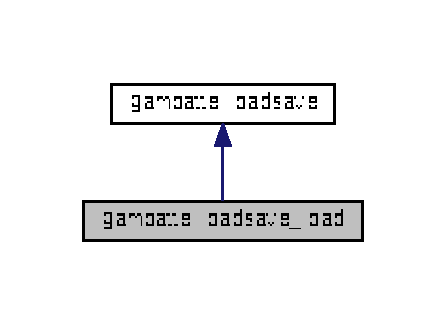
\includegraphics[width=214pt]{classgambatte_1_1loadsave__load__inherit__graph}
\end{center}
\end{figure}


Collaboration diagram for gambatte\+:\+:loadsave\+\_\+load\+:\nopagebreak
\begin{figure}[H]
\begin{center}
\leavevmode
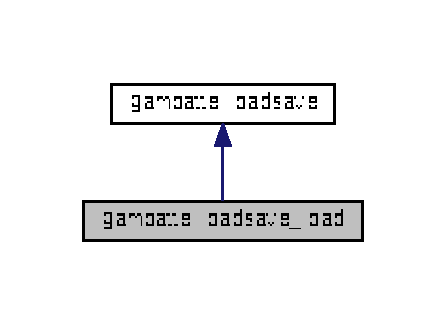
\includegraphics[width=214pt]{classgambatte_1_1loadsave__load__coll__graph}
\end{center}
\end{figure}
\subsection*{Public Member Functions}
\begin{DoxyCompactItemize}
\item 
\hyperlink{classgambatte_1_1loadsave__load_a8a06e288abaaf2196cf2bfe9ad5c1615}{loadsave\+\_\+load} (const std\+::vector$<$ char $>$ \&\+\_\+memory)
\item 
\hyperlink{classgambatte_1_1loadsave__load_a5d635194474a2c4e315e2dddd5e8f116}{$\sim$loadsave\+\_\+load} ()  throw ()
\item 
void \hyperlink{classgambatte_1_1loadsave__load_a551d7c208300ff066c9725c3efff8aa9}{operator()} (bool \&x)
\item 
void \hyperlink{classgambatte_1_1loadsave__load_ae0135e997f4fac56481edb91a3b4e6c0}{operator()} (signed char \&x)
\item 
void \hyperlink{classgambatte_1_1loadsave__load_a1e6642fca66ae4b43af93815c69d5aba}{operator()} (unsigned char \&x)
\item 
void \hyperlink{classgambatte_1_1loadsave__load_aac3a5c1c4086659f211772d161fb766f}{operator()} (signed short \&x)
\item 
void \hyperlink{classgambatte_1_1loadsave__load_a5350f167b32445f8079dff6d821f91e9}{operator()} (unsigned short \&x)
\item 
void \hyperlink{classgambatte_1_1loadsave__load_ae2291b82a8512c04091f59170e7a866f}{operator()} (signed \hyperlink{ioapi_8h_a787fa3cf048117ba7123753c1e74fcd6}{int} \&x)
\item 
void \hyperlink{classgambatte_1_1loadsave__load_a19ccef4878489e15440e27c0f0614de5}{operator()} (unsigned \hyperlink{ioapi_8h_a787fa3cf048117ba7123753c1e74fcd6}{int} \&x)
\item 
void \hyperlink{classgambatte_1_1loadsave__load_a8102bdbd866f6a0a05273496bed7ed90}{operator()} (signed \hyperlink{ioapi_8h_a3c7b35ad9dab18b8310343c201f7b27e}{long} \hyperlink{ioapi_8h_a3c7b35ad9dab18b8310343c201f7b27e}{long} \&x)
\item 
void \hyperlink{classgambatte_1_1loadsave__load_a18686dd69eb8623d5e4d63f45a4ff7ef}{operator()} (unsigned \hyperlink{ioapi_8h_a3c7b35ad9dab18b8310343c201f7b27e}{long} \hyperlink{ioapi_8h_a3c7b35ad9dab18b8310343c201f7b27e}{long} \&x)
\item 
void \hyperlink{classgambatte_1_1loadsave__load_a0d08f451690c66586668b1e7c4f87fde}{operator()} (signed char $\ast$x, size\+\_\+t s)
\item 
void \hyperlink{classgambatte_1_1loadsave__load_aabf9a95ede92c9905c3ff6ba6cf49e0e}{operator()} (unsigned char $\ast$x, size\+\_\+t s)
\item 
void \hyperlink{classgambatte_1_1loadsave__load_a7123df06b1844de40a70de8acb6f4a20}{operator()} (signed short $\ast$x, size\+\_\+t s)
\item 
void \hyperlink{classgambatte_1_1loadsave__load_a0a45f5a10b88dac757b14fe0c0ebfce6}{operator()} (unsigned short $\ast$x, size\+\_\+t s)
\item 
void \hyperlink{classgambatte_1_1loadsave__load_a3ea605ff0d7fa8d09e57c02d444b8850}{operator()} (signed \hyperlink{ioapi_8h_a787fa3cf048117ba7123753c1e74fcd6}{int} $\ast$x, size\+\_\+t s)
\item 
void \hyperlink{classgambatte_1_1loadsave__load_a8a358ad29b9df4d704cebe61585df877}{operator()} (unsigned \hyperlink{ioapi_8h_a787fa3cf048117ba7123753c1e74fcd6}{int} $\ast$x, size\+\_\+t s)
\item 
void \hyperlink{classgambatte_1_1loadsave__load_a0d28f32c599ce42adf51dc1cfe607123}{operator()} (signed \hyperlink{ioapi_8h_a3c7b35ad9dab18b8310343c201f7b27e}{long} \hyperlink{ioapi_8h_a3c7b35ad9dab18b8310343c201f7b27e}{long} $\ast$x, size\+\_\+t s)
\item 
void \hyperlink{classgambatte_1_1loadsave__load_a3ac6797ca2311f63b2f4ec080de5f1d9}{operator()} (unsigned \hyperlink{ioapi_8h_a3c7b35ad9dab18b8310343c201f7b27e}{long} \hyperlink{ioapi_8h_a3c7b35ad9dab18b8310343c201f7b27e}{long} $\ast$x, size\+\_\+t s)
\item 
void \hyperlink{classgambatte_1_1loadsave__load_aa2d8402dc6fdececfd223520fc9cf0d8}{operator()} (unsigned char $\ast$\&\hyperlink{classgambatte_1_1loadsave__load_ab49af43a813936002e9adb21103beae8}{ptr}, unsigned char $\ast$abase)
\item 
void \hyperlink{classgambatte_1_1loadsave__load_a58313e7e62236560888348cf8e779cb0}{operator()} (const unsigned char $\ast$\&\hyperlink{classgambatte_1_1loadsave__load_ab49af43a813936002e9adb21103beae8}{ptr}, unsigned char $\ast$abase)
\item 
void \hyperlink{classgambatte_1_1loadsave__load_a85b86aaebae87da4bead8d3ed4ac3a9c}{tag} (unsigned short \+\_\+tag)
\item 
bool \hyperlink{classgambatte_1_1loadsave__load_a2ac8e306cef4eab6a804deab9e853fd3}{saving} ()
\end{DoxyCompactItemize}
\subsection*{Private Member Functions}
\begin{DoxyCompactItemize}
\item 
{\footnotesize template$<$typename T $>$ }\\void \hyperlink{classgambatte_1_1loadsave__load_a45e10c2b20eea19e3b92fe0560c5e107}{do\+\_\+op} (T \&x)
\item 
{\footnotesize template$<$typename T $>$ }\\void \hyperlink{classgambatte_1_1loadsave__load_adff7d2df0225532d464ea7d9f9d1458a}{do\+\_\+op} (T \&x, unsigned char \+\_\+tag)
\item 
{\footnotesize template$<$typename T $>$ }\\void \hyperlink{classgambatte_1_1loadsave__load_a9f958d9dff1f36f82b393c8cf4c734cb}{do\+\_\+op} (T $\ast$x, size\+\_\+t s, unsigned char \+\_\+tag)
\end{DoxyCompactItemize}
\subsection*{Private Attributes}
\begin{DoxyCompactItemize}
\item 
const std\+::vector$<$ char $>$ \& \hyperlink{classgambatte_1_1loadsave__load_aaf91faa9fd5d0ce6d4ff3d4e7749ce1d}{memory}
\item 
size\+\_\+t \hyperlink{classgambatte_1_1loadsave__load_ab49af43a813936002e9adb21103beae8}{ptr}
\end{DoxyCompactItemize}


\subsection{Constructor \& Destructor Documentation}
\mbox{\Hypertarget{classgambatte_1_1loadsave__load_a8a06e288abaaf2196cf2bfe9ad5c1615}\label{classgambatte_1_1loadsave__load_a8a06e288abaaf2196cf2bfe9ad5c1615}} 
\index{gambatte\+::loadsave\+\_\+load@{gambatte\+::loadsave\+\_\+load}!loadsave\+\_\+load@{loadsave\+\_\+load}}
\index{loadsave\+\_\+load@{loadsave\+\_\+load}!gambatte\+::loadsave\+\_\+load@{gambatte\+::loadsave\+\_\+load}}
\subsubsection{\texorpdfstring{loadsave\+\_\+load()}{loadsave\_load()}}
{\footnotesize\ttfamily gambatte\+::loadsave\+\_\+load\+::loadsave\+\_\+load (\begin{DoxyParamCaption}\item[{const std\+::vector$<$ char $>$ \&}]{\+\_\+memory }\end{DoxyParamCaption})}

\mbox{\Hypertarget{classgambatte_1_1loadsave__load_a5d635194474a2c4e315e2dddd5e8f116}\label{classgambatte_1_1loadsave__load_a5d635194474a2c4e315e2dddd5e8f116}} 
\index{gambatte\+::loadsave\+\_\+load@{gambatte\+::loadsave\+\_\+load}!````~loadsave\+\_\+load@{$\sim$loadsave\+\_\+load}}
\index{````~loadsave\+\_\+load@{$\sim$loadsave\+\_\+load}!gambatte\+::loadsave\+\_\+load@{gambatte\+::loadsave\+\_\+load}}
\subsubsection{\texorpdfstring{$\sim$loadsave\+\_\+load()}{~loadsave\_load()}}
{\footnotesize\ttfamily gambatte\+::loadsave\+\_\+load\+::$\sim$loadsave\+\_\+load (\begin{DoxyParamCaption}{ }\end{DoxyParamCaption}) throw  ) }



\subsection{Member Function Documentation}
\mbox{\Hypertarget{classgambatte_1_1loadsave__load_a45e10c2b20eea19e3b92fe0560c5e107}\label{classgambatte_1_1loadsave__load_a45e10c2b20eea19e3b92fe0560c5e107}} 
\index{gambatte\+::loadsave\+\_\+load@{gambatte\+::loadsave\+\_\+load}!do\+\_\+op@{do\+\_\+op}}
\index{do\+\_\+op@{do\+\_\+op}!gambatte\+::loadsave\+\_\+load@{gambatte\+::loadsave\+\_\+load}}
\subsubsection{\texorpdfstring{do\+\_\+op()}{do\_op()}\hspace{0.1cm}{\footnotesize\ttfamily [1/3]}}
{\footnotesize\ttfamily template$<$typename T $>$ \\
void gambatte\+::loadsave\+\_\+load\+::do\+\_\+op (\begin{DoxyParamCaption}\item[{T \&}]{x }\end{DoxyParamCaption})\hspace{0.3cm}{\ttfamily [inline]}, {\ttfamily [private]}}

\mbox{\Hypertarget{classgambatte_1_1loadsave__load_adff7d2df0225532d464ea7d9f9d1458a}\label{classgambatte_1_1loadsave__load_adff7d2df0225532d464ea7d9f9d1458a}} 
\index{gambatte\+::loadsave\+\_\+load@{gambatte\+::loadsave\+\_\+load}!do\+\_\+op@{do\+\_\+op}}
\index{do\+\_\+op@{do\+\_\+op}!gambatte\+::loadsave\+\_\+load@{gambatte\+::loadsave\+\_\+load}}
\subsubsection{\texorpdfstring{do\+\_\+op()}{do\_op()}\hspace{0.1cm}{\footnotesize\ttfamily [2/3]}}
{\footnotesize\ttfamily template$<$typename T $>$ \\
void gambatte\+::loadsave\+\_\+load\+::do\+\_\+op (\begin{DoxyParamCaption}\item[{T \&}]{x,  }\item[{unsigned char}]{\+\_\+tag }\end{DoxyParamCaption})\hspace{0.3cm}{\ttfamily [inline]}, {\ttfamily [private]}}

\mbox{\Hypertarget{classgambatte_1_1loadsave__load_a9f958d9dff1f36f82b393c8cf4c734cb}\label{classgambatte_1_1loadsave__load_a9f958d9dff1f36f82b393c8cf4c734cb}} 
\index{gambatte\+::loadsave\+\_\+load@{gambatte\+::loadsave\+\_\+load}!do\+\_\+op@{do\+\_\+op}}
\index{do\+\_\+op@{do\+\_\+op}!gambatte\+::loadsave\+\_\+load@{gambatte\+::loadsave\+\_\+load}}
\subsubsection{\texorpdfstring{do\+\_\+op()}{do\_op()}\hspace{0.1cm}{\footnotesize\ttfamily [3/3]}}
{\footnotesize\ttfamily template$<$typename T $>$ \\
void gambatte\+::loadsave\+\_\+load\+::do\+\_\+op (\begin{DoxyParamCaption}\item[{T $\ast$}]{x,  }\item[{size\+\_\+t}]{s,  }\item[{unsigned char}]{\+\_\+tag }\end{DoxyParamCaption})\hspace{0.3cm}{\ttfamily [private]}}

\mbox{\Hypertarget{classgambatte_1_1loadsave__load_a551d7c208300ff066c9725c3efff8aa9}\label{classgambatte_1_1loadsave__load_a551d7c208300ff066c9725c3efff8aa9}} 
\index{gambatte\+::loadsave\+\_\+load@{gambatte\+::loadsave\+\_\+load}!operator()@{operator()}}
\index{operator()@{operator()}!gambatte\+::loadsave\+\_\+load@{gambatte\+::loadsave\+\_\+load}}
\subsubsection{\texorpdfstring{operator()()}{operator()()}\hspace{0.1cm}{\footnotesize\ttfamily [1/19]}}
{\footnotesize\ttfamily void gambatte\+::loadsave\+\_\+load\+::operator() (\begin{DoxyParamCaption}\item[{bool \&}]{x }\end{DoxyParamCaption})\hspace{0.3cm}{\ttfamily [virtual]}}



Implements \hyperlink{classgambatte_1_1loadsave_a286a1bc924db345dda227a735a5ba038}{gambatte\+::loadsave}.

\mbox{\Hypertarget{classgambatte_1_1loadsave__load_ae0135e997f4fac56481edb91a3b4e6c0}\label{classgambatte_1_1loadsave__load_ae0135e997f4fac56481edb91a3b4e6c0}} 
\index{gambatte\+::loadsave\+\_\+load@{gambatte\+::loadsave\+\_\+load}!operator()@{operator()}}
\index{operator()@{operator()}!gambatte\+::loadsave\+\_\+load@{gambatte\+::loadsave\+\_\+load}}
\subsubsection{\texorpdfstring{operator()()}{operator()()}\hspace{0.1cm}{\footnotesize\ttfamily [2/19]}}
{\footnotesize\ttfamily void gambatte\+::loadsave\+\_\+load\+::operator() (\begin{DoxyParamCaption}\item[{signed char \&}]{x }\end{DoxyParamCaption})\hspace{0.3cm}{\ttfamily [virtual]}}



Implements \hyperlink{classgambatte_1_1loadsave_abe43ebb74162f066b542781f5ec7e5af}{gambatte\+::loadsave}.

\mbox{\Hypertarget{classgambatte_1_1loadsave__load_a1e6642fca66ae4b43af93815c69d5aba}\label{classgambatte_1_1loadsave__load_a1e6642fca66ae4b43af93815c69d5aba}} 
\index{gambatte\+::loadsave\+\_\+load@{gambatte\+::loadsave\+\_\+load}!operator()@{operator()}}
\index{operator()@{operator()}!gambatte\+::loadsave\+\_\+load@{gambatte\+::loadsave\+\_\+load}}
\subsubsection{\texorpdfstring{operator()()}{operator()()}\hspace{0.1cm}{\footnotesize\ttfamily [3/19]}}
{\footnotesize\ttfamily void gambatte\+::loadsave\+\_\+load\+::operator() (\begin{DoxyParamCaption}\item[{unsigned char \&}]{x }\end{DoxyParamCaption})\hspace{0.3cm}{\ttfamily [virtual]}}



Implements \hyperlink{classgambatte_1_1loadsave_a475286c3cdfc0a207cd6ac9d27bf5b0b}{gambatte\+::loadsave}.

\mbox{\Hypertarget{classgambatte_1_1loadsave__load_aac3a5c1c4086659f211772d161fb766f}\label{classgambatte_1_1loadsave__load_aac3a5c1c4086659f211772d161fb766f}} 
\index{gambatte\+::loadsave\+\_\+load@{gambatte\+::loadsave\+\_\+load}!operator()@{operator()}}
\index{operator()@{operator()}!gambatte\+::loadsave\+\_\+load@{gambatte\+::loadsave\+\_\+load}}
\subsubsection{\texorpdfstring{operator()()}{operator()()}\hspace{0.1cm}{\footnotesize\ttfamily [4/19]}}
{\footnotesize\ttfamily void gambatte\+::loadsave\+\_\+load\+::operator() (\begin{DoxyParamCaption}\item[{signed short \&}]{x }\end{DoxyParamCaption})\hspace{0.3cm}{\ttfamily [virtual]}}



Implements \hyperlink{classgambatte_1_1loadsave_a8874e92f76b3765efba593c377667f16}{gambatte\+::loadsave}.

\mbox{\Hypertarget{classgambatte_1_1loadsave__load_a5350f167b32445f8079dff6d821f91e9}\label{classgambatte_1_1loadsave__load_a5350f167b32445f8079dff6d821f91e9}} 
\index{gambatte\+::loadsave\+\_\+load@{gambatte\+::loadsave\+\_\+load}!operator()@{operator()}}
\index{operator()@{operator()}!gambatte\+::loadsave\+\_\+load@{gambatte\+::loadsave\+\_\+load}}
\subsubsection{\texorpdfstring{operator()()}{operator()()}\hspace{0.1cm}{\footnotesize\ttfamily [5/19]}}
{\footnotesize\ttfamily void gambatte\+::loadsave\+\_\+load\+::operator() (\begin{DoxyParamCaption}\item[{unsigned short \&}]{x }\end{DoxyParamCaption})\hspace{0.3cm}{\ttfamily [virtual]}}



Implements \hyperlink{classgambatte_1_1loadsave_a36c04339183e08d7dbfa0aeabc3c953d}{gambatte\+::loadsave}.

\mbox{\Hypertarget{classgambatte_1_1loadsave__load_ae2291b82a8512c04091f59170e7a866f}\label{classgambatte_1_1loadsave__load_ae2291b82a8512c04091f59170e7a866f}} 
\index{gambatte\+::loadsave\+\_\+load@{gambatte\+::loadsave\+\_\+load}!operator()@{operator()}}
\index{operator()@{operator()}!gambatte\+::loadsave\+\_\+load@{gambatte\+::loadsave\+\_\+load}}
\subsubsection{\texorpdfstring{operator()()}{operator()()}\hspace{0.1cm}{\footnotesize\ttfamily [6/19]}}
{\footnotesize\ttfamily void gambatte\+::loadsave\+\_\+load\+::operator() (\begin{DoxyParamCaption}\item[{signed \hyperlink{ioapi_8h_a787fa3cf048117ba7123753c1e74fcd6}{int} \&}]{x }\end{DoxyParamCaption})\hspace{0.3cm}{\ttfamily [virtual]}}



Implements \hyperlink{classgambatte_1_1loadsave_a9a8e8765ac066a4d51099147f71595d1}{gambatte\+::loadsave}.

\mbox{\Hypertarget{classgambatte_1_1loadsave__load_a19ccef4878489e15440e27c0f0614de5}\label{classgambatte_1_1loadsave__load_a19ccef4878489e15440e27c0f0614de5}} 
\index{gambatte\+::loadsave\+\_\+load@{gambatte\+::loadsave\+\_\+load}!operator()@{operator()}}
\index{operator()@{operator()}!gambatte\+::loadsave\+\_\+load@{gambatte\+::loadsave\+\_\+load}}
\subsubsection{\texorpdfstring{operator()()}{operator()()}\hspace{0.1cm}{\footnotesize\ttfamily [7/19]}}
{\footnotesize\ttfamily void gambatte\+::loadsave\+\_\+load\+::operator() (\begin{DoxyParamCaption}\item[{unsigned \hyperlink{ioapi_8h_a787fa3cf048117ba7123753c1e74fcd6}{int} \&}]{x }\end{DoxyParamCaption})\hspace{0.3cm}{\ttfamily [virtual]}}



Implements \hyperlink{classgambatte_1_1loadsave_a263bbb4b470594752ca94548673e66a4}{gambatte\+::loadsave}.

\mbox{\Hypertarget{classgambatte_1_1loadsave__load_a8102bdbd866f6a0a05273496bed7ed90}\label{classgambatte_1_1loadsave__load_a8102bdbd866f6a0a05273496bed7ed90}} 
\index{gambatte\+::loadsave\+\_\+load@{gambatte\+::loadsave\+\_\+load}!operator()@{operator()}}
\index{operator()@{operator()}!gambatte\+::loadsave\+\_\+load@{gambatte\+::loadsave\+\_\+load}}
\subsubsection{\texorpdfstring{operator()()}{operator()()}\hspace{0.1cm}{\footnotesize\ttfamily [8/19]}}
{\footnotesize\ttfamily void gambatte\+::loadsave\+\_\+load\+::operator() (\begin{DoxyParamCaption}\item[{signed \hyperlink{ioapi_8h_a3c7b35ad9dab18b8310343c201f7b27e}{long} \hyperlink{ioapi_8h_a3c7b35ad9dab18b8310343c201f7b27e}{long} \&}]{x }\end{DoxyParamCaption})\hspace{0.3cm}{\ttfamily [virtual]}}



Implements \hyperlink{classgambatte_1_1loadsave_a882deed58830a077498c160ba2870eec}{gambatte\+::loadsave}.

\mbox{\Hypertarget{classgambatte_1_1loadsave__load_a18686dd69eb8623d5e4d63f45a4ff7ef}\label{classgambatte_1_1loadsave__load_a18686dd69eb8623d5e4d63f45a4ff7ef}} 
\index{gambatte\+::loadsave\+\_\+load@{gambatte\+::loadsave\+\_\+load}!operator()@{operator()}}
\index{operator()@{operator()}!gambatte\+::loadsave\+\_\+load@{gambatte\+::loadsave\+\_\+load}}
\subsubsection{\texorpdfstring{operator()()}{operator()()}\hspace{0.1cm}{\footnotesize\ttfamily [9/19]}}
{\footnotesize\ttfamily void gambatte\+::loadsave\+\_\+load\+::operator() (\begin{DoxyParamCaption}\item[{unsigned \hyperlink{ioapi_8h_a3c7b35ad9dab18b8310343c201f7b27e}{long} \hyperlink{ioapi_8h_a3c7b35ad9dab18b8310343c201f7b27e}{long} \&}]{x }\end{DoxyParamCaption})\hspace{0.3cm}{\ttfamily [virtual]}}



Implements \hyperlink{classgambatte_1_1loadsave_aca5dcc05e845b6aa3086065048ab6e29}{gambatte\+::loadsave}.

\mbox{\Hypertarget{classgambatte_1_1loadsave__load_a0d08f451690c66586668b1e7c4f87fde}\label{classgambatte_1_1loadsave__load_a0d08f451690c66586668b1e7c4f87fde}} 
\index{gambatte\+::loadsave\+\_\+load@{gambatte\+::loadsave\+\_\+load}!operator()@{operator()}}
\index{operator()@{operator()}!gambatte\+::loadsave\+\_\+load@{gambatte\+::loadsave\+\_\+load}}
\subsubsection{\texorpdfstring{operator()()}{operator()()}\hspace{0.1cm}{\footnotesize\ttfamily [10/19]}}
{\footnotesize\ttfamily void gambatte\+::loadsave\+\_\+load\+::operator() (\begin{DoxyParamCaption}\item[{signed char $\ast$}]{x,  }\item[{size\+\_\+t}]{s }\end{DoxyParamCaption})\hspace{0.3cm}{\ttfamily [virtual]}}



Implements \hyperlink{classgambatte_1_1loadsave_a8ba29ce3f56dbaa7ac1d4aec4b705af3}{gambatte\+::loadsave}.

\mbox{\Hypertarget{classgambatte_1_1loadsave__load_aabf9a95ede92c9905c3ff6ba6cf49e0e}\label{classgambatte_1_1loadsave__load_aabf9a95ede92c9905c3ff6ba6cf49e0e}} 
\index{gambatte\+::loadsave\+\_\+load@{gambatte\+::loadsave\+\_\+load}!operator()@{operator()}}
\index{operator()@{operator()}!gambatte\+::loadsave\+\_\+load@{gambatte\+::loadsave\+\_\+load}}
\subsubsection{\texorpdfstring{operator()()}{operator()()}\hspace{0.1cm}{\footnotesize\ttfamily [11/19]}}
{\footnotesize\ttfamily void gambatte\+::loadsave\+\_\+load\+::operator() (\begin{DoxyParamCaption}\item[{unsigned char $\ast$}]{x,  }\item[{size\+\_\+t}]{s }\end{DoxyParamCaption})\hspace{0.3cm}{\ttfamily [virtual]}}



Implements \hyperlink{classgambatte_1_1loadsave_ae1ab673c435463f83c510446d7455436}{gambatte\+::loadsave}.

\mbox{\Hypertarget{classgambatte_1_1loadsave__load_a7123df06b1844de40a70de8acb6f4a20}\label{classgambatte_1_1loadsave__load_a7123df06b1844de40a70de8acb6f4a20}} 
\index{gambatte\+::loadsave\+\_\+load@{gambatte\+::loadsave\+\_\+load}!operator()@{operator()}}
\index{operator()@{operator()}!gambatte\+::loadsave\+\_\+load@{gambatte\+::loadsave\+\_\+load}}
\subsubsection{\texorpdfstring{operator()()}{operator()()}\hspace{0.1cm}{\footnotesize\ttfamily [12/19]}}
{\footnotesize\ttfamily void gambatte\+::loadsave\+\_\+load\+::operator() (\begin{DoxyParamCaption}\item[{signed short $\ast$}]{x,  }\item[{size\+\_\+t}]{s }\end{DoxyParamCaption})\hspace{0.3cm}{\ttfamily [virtual]}}



Implements \hyperlink{classgambatte_1_1loadsave_ac30751838bea28e3e266da5194b429d1}{gambatte\+::loadsave}.

\mbox{\Hypertarget{classgambatte_1_1loadsave__load_a0a45f5a10b88dac757b14fe0c0ebfce6}\label{classgambatte_1_1loadsave__load_a0a45f5a10b88dac757b14fe0c0ebfce6}} 
\index{gambatte\+::loadsave\+\_\+load@{gambatte\+::loadsave\+\_\+load}!operator()@{operator()}}
\index{operator()@{operator()}!gambatte\+::loadsave\+\_\+load@{gambatte\+::loadsave\+\_\+load}}
\subsubsection{\texorpdfstring{operator()()}{operator()()}\hspace{0.1cm}{\footnotesize\ttfamily [13/19]}}
{\footnotesize\ttfamily void gambatte\+::loadsave\+\_\+load\+::operator() (\begin{DoxyParamCaption}\item[{unsigned short $\ast$}]{x,  }\item[{size\+\_\+t}]{s }\end{DoxyParamCaption})\hspace{0.3cm}{\ttfamily [virtual]}}



Implements \hyperlink{classgambatte_1_1loadsave_aa260c68090c6bb3b5620ac77ce70815d}{gambatte\+::loadsave}.

\mbox{\Hypertarget{classgambatte_1_1loadsave__load_a3ea605ff0d7fa8d09e57c02d444b8850}\label{classgambatte_1_1loadsave__load_a3ea605ff0d7fa8d09e57c02d444b8850}} 
\index{gambatte\+::loadsave\+\_\+load@{gambatte\+::loadsave\+\_\+load}!operator()@{operator()}}
\index{operator()@{operator()}!gambatte\+::loadsave\+\_\+load@{gambatte\+::loadsave\+\_\+load}}
\subsubsection{\texorpdfstring{operator()()}{operator()()}\hspace{0.1cm}{\footnotesize\ttfamily [14/19]}}
{\footnotesize\ttfamily void gambatte\+::loadsave\+\_\+load\+::operator() (\begin{DoxyParamCaption}\item[{signed \hyperlink{ioapi_8h_a787fa3cf048117ba7123753c1e74fcd6}{int} $\ast$}]{x,  }\item[{size\+\_\+t}]{s }\end{DoxyParamCaption})\hspace{0.3cm}{\ttfamily [virtual]}}



Implements \hyperlink{classgambatte_1_1loadsave_a9f843edffc4473365246e8620d65f1e3}{gambatte\+::loadsave}.

\mbox{\Hypertarget{classgambatte_1_1loadsave__load_a8a358ad29b9df4d704cebe61585df877}\label{classgambatte_1_1loadsave__load_a8a358ad29b9df4d704cebe61585df877}} 
\index{gambatte\+::loadsave\+\_\+load@{gambatte\+::loadsave\+\_\+load}!operator()@{operator()}}
\index{operator()@{operator()}!gambatte\+::loadsave\+\_\+load@{gambatte\+::loadsave\+\_\+load}}
\subsubsection{\texorpdfstring{operator()()}{operator()()}\hspace{0.1cm}{\footnotesize\ttfamily [15/19]}}
{\footnotesize\ttfamily void gambatte\+::loadsave\+\_\+load\+::operator() (\begin{DoxyParamCaption}\item[{unsigned \hyperlink{ioapi_8h_a787fa3cf048117ba7123753c1e74fcd6}{int} $\ast$}]{x,  }\item[{size\+\_\+t}]{s }\end{DoxyParamCaption})\hspace{0.3cm}{\ttfamily [virtual]}}



Implements \hyperlink{classgambatte_1_1loadsave_a0985be7f430a1626e2b0f47066e9a8b6}{gambatte\+::loadsave}.

\mbox{\Hypertarget{classgambatte_1_1loadsave__load_a0d28f32c599ce42adf51dc1cfe607123}\label{classgambatte_1_1loadsave__load_a0d28f32c599ce42adf51dc1cfe607123}} 
\index{gambatte\+::loadsave\+\_\+load@{gambatte\+::loadsave\+\_\+load}!operator()@{operator()}}
\index{operator()@{operator()}!gambatte\+::loadsave\+\_\+load@{gambatte\+::loadsave\+\_\+load}}
\subsubsection{\texorpdfstring{operator()()}{operator()()}\hspace{0.1cm}{\footnotesize\ttfamily [16/19]}}
{\footnotesize\ttfamily void gambatte\+::loadsave\+\_\+load\+::operator() (\begin{DoxyParamCaption}\item[{signed \hyperlink{ioapi_8h_a3c7b35ad9dab18b8310343c201f7b27e}{long} \hyperlink{ioapi_8h_a3c7b35ad9dab18b8310343c201f7b27e}{long} $\ast$}]{x,  }\item[{size\+\_\+t}]{s }\end{DoxyParamCaption})}

\mbox{\Hypertarget{classgambatte_1_1loadsave__load_a3ac6797ca2311f63b2f4ec080de5f1d9}\label{classgambatte_1_1loadsave__load_a3ac6797ca2311f63b2f4ec080de5f1d9}} 
\index{gambatte\+::loadsave\+\_\+load@{gambatte\+::loadsave\+\_\+load}!operator()@{operator()}}
\index{operator()@{operator()}!gambatte\+::loadsave\+\_\+load@{gambatte\+::loadsave\+\_\+load}}
\subsubsection{\texorpdfstring{operator()()}{operator()()}\hspace{0.1cm}{\footnotesize\ttfamily [17/19]}}
{\footnotesize\ttfamily void gambatte\+::loadsave\+\_\+load\+::operator() (\begin{DoxyParamCaption}\item[{unsigned \hyperlink{ioapi_8h_a3c7b35ad9dab18b8310343c201f7b27e}{long} \hyperlink{ioapi_8h_a3c7b35ad9dab18b8310343c201f7b27e}{long} $\ast$}]{x,  }\item[{size\+\_\+t}]{s }\end{DoxyParamCaption})\hspace{0.3cm}{\ttfamily [virtual]}}



Implements \hyperlink{classgambatte_1_1loadsave_a93ef67515dbf61461e7370c9cc77c8a6}{gambatte\+::loadsave}.

\mbox{\Hypertarget{classgambatte_1_1loadsave__load_aa2d8402dc6fdececfd223520fc9cf0d8}\label{classgambatte_1_1loadsave__load_aa2d8402dc6fdececfd223520fc9cf0d8}} 
\index{gambatte\+::loadsave\+\_\+load@{gambatte\+::loadsave\+\_\+load}!operator()@{operator()}}
\index{operator()@{operator()}!gambatte\+::loadsave\+\_\+load@{gambatte\+::loadsave\+\_\+load}}
\subsubsection{\texorpdfstring{operator()()}{operator()()}\hspace{0.1cm}{\footnotesize\ttfamily [18/19]}}
{\footnotesize\ttfamily void gambatte\+::loadsave\+\_\+load\+::operator() (\begin{DoxyParamCaption}\item[{unsigned char $\ast$\&}]{ptr,  }\item[{unsigned char $\ast$}]{abase }\end{DoxyParamCaption})\hspace{0.3cm}{\ttfamily [virtual]}}



Implements \hyperlink{classgambatte_1_1loadsave_a911a5ce78fbb8c4ceb36984a9967ea72}{gambatte\+::loadsave}.

\mbox{\Hypertarget{classgambatte_1_1loadsave__load_a58313e7e62236560888348cf8e779cb0}\label{classgambatte_1_1loadsave__load_a58313e7e62236560888348cf8e779cb0}} 
\index{gambatte\+::loadsave\+\_\+load@{gambatte\+::loadsave\+\_\+load}!operator()@{operator()}}
\index{operator()@{operator()}!gambatte\+::loadsave\+\_\+load@{gambatte\+::loadsave\+\_\+load}}
\subsubsection{\texorpdfstring{operator()()}{operator()()}\hspace{0.1cm}{\footnotesize\ttfamily [19/19]}}
{\footnotesize\ttfamily void gambatte\+::loadsave\+\_\+load\+::operator() (\begin{DoxyParamCaption}\item[{const unsigned char $\ast$\&}]{ptr,  }\item[{unsigned char $\ast$}]{abase }\end{DoxyParamCaption})\hspace{0.3cm}{\ttfamily [virtual]}}



Implements \hyperlink{classgambatte_1_1loadsave_a57518c27d7844ae48faea91fc04a680a}{gambatte\+::loadsave}.

\mbox{\Hypertarget{classgambatte_1_1loadsave__load_a2ac8e306cef4eab6a804deab9e853fd3}\label{classgambatte_1_1loadsave__load_a2ac8e306cef4eab6a804deab9e853fd3}} 
\index{gambatte\+::loadsave\+\_\+load@{gambatte\+::loadsave\+\_\+load}!saving@{saving}}
\index{saving@{saving}!gambatte\+::loadsave\+\_\+load@{gambatte\+::loadsave\+\_\+load}}
\subsubsection{\texorpdfstring{saving()}{saving()}}
{\footnotesize\ttfamily bool gambatte\+::loadsave\+\_\+load\+::saving (\begin{DoxyParamCaption}{ }\end{DoxyParamCaption})\hspace{0.3cm}{\ttfamily [virtual]}}



Implements \hyperlink{classgambatte_1_1loadsave_a0a05b67eadfbb26f654f3d5ec287c652}{gambatte\+::loadsave}.

\mbox{\Hypertarget{classgambatte_1_1loadsave__load_a85b86aaebae87da4bead8d3ed4ac3a9c}\label{classgambatte_1_1loadsave__load_a85b86aaebae87da4bead8d3ed4ac3a9c}} 
\index{gambatte\+::loadsave\+\_\+load@{gambatte\+::loadsave\+\_\+load}!tag@{tag}}
\index{tag@{tag}!gambatte\+::loadsave\+\_\+load@{gambatte\+::loadsave\+\_\+load}}
\subsubsection{\texorpdfstring{tag()}{tag()}}
{\footnotesize\ttfamily void gambatte\+::loadsave\+\_\+load\+::tag (\begin{DoxyParamCaption}\item[{unsigned short}]{\+\_\+tag }\end{DoxyParamCaption})\hspace{0.3cm}{\ttfamily [virtual]}}



Implements \hyperlink{classgambatte_1_1loadsave_af4a635fc49c23e53e48b2b9d320aa165}{gambatte\+::loadsave}.



\subsection{Member Data Documentation}
\mbox{\Hypertarget{classgambatte_1_1loadsave__load_aaf91faa9fd5d0ce6d4ff3d4e7749ce1d}\label{classgambatte_1_1loadsave__load_aaf91faa9fd5d0ce6d4ff3d4e7749ce1d}} 
\index{gambatte\+::loadsave\+\_\+load@{gambatte\+::loadsave\+\_\+load}!memory@{memory}}
\index{memory@{memory}!gambatte\+::loadsave\+\_\+load@{gambatte\+::loadsave\+\_\+load}}
\subsubsection{\texorpdfstring{memory}{memory}}
{\footnotesize\ttfamily const std\+::vector$<$char$>$\& gambatte\+::loadsave\+\_\+load\+::memory\hspace{0.3cm}{\ttfamily [private]}}

\mbox{\Hypertarget{classgambatte_1_1loadsave__load_ab49af43a813936002e9adb21103beae8}\label{classgambatte_1_1loadsave__load_ab49af43a813936002e9adb21103beae8}} 
\index{gambatte\+::loadsave\+\_\+load@{gambatte\+::loadsave\+\_\+load}!ptr@{ptr}}
\index{ptr@{ptr}!gambatte\+::loadsave\+\_\+load@{gambatte\+::loadsave\+\_\+load}}
\subsubsection{\texorpdfstring{ptr}{ptr}}
{\footnotesize\ttfamily size\+\_\+t gambatte\+::loadsave\+\_\+load\+::ptr\hspace{0.3cm}{\ttfamily [private]}}



The documentation for this class was generated from the following files\+:\begin{DoxyCompactItemize}
\item 
src/\hyperlink{loadsave_8h}{loadsave.\+h}\item 
src/\hyperlink{loadsave_8cpp}{loadsave.\+cpp}\end{DoxyCompactItemize}

\hypertarget{classgambatte_1_1loadsave__save}{}\section{gambatte\+:\+:loadsave\+\_\+save Class Reference}
\label{classgambatte_1_1loadsave__save}\index{gambatte\+::loadsave\+\_\+save@{gambatte\+::loadsave\+\_\+save}}


{\ttfamily \#include $<$loadsave.\+h$>$}



Inheritance diagram for gambatte\+:\+:loadsave\+\_\+save\+:\nopagebreak
\begin{figure}[H]
\begin{center}
\leavevmode
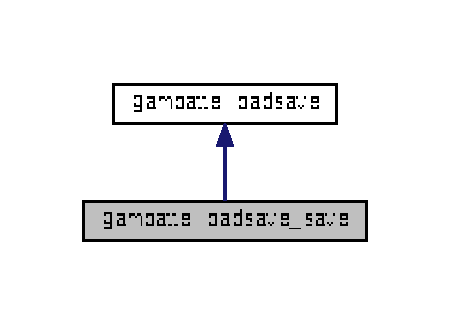
\includegraphics[width=216pt]{classgambatte_1_1loadsave__save__inherit__graph}
\end{center}
\end{figure}


Collaboration diagram for gambatte\+:\+:loadsave\+\_\+save\+:\nopagebreak
\begin{figure}[H]
\begin{center}
\leavevmode
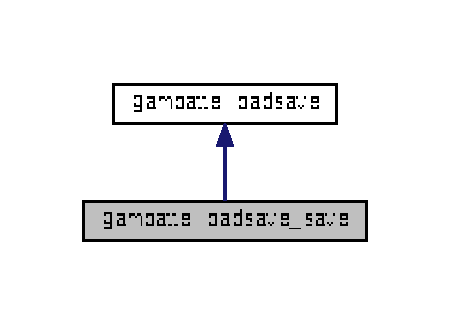
\includegraphics[width=216pt]{classgambatte_1_1loadsave__save__coll__graph}
\end{center}
\end{figure}
\subsection*{Public Member Functions}
\begin{DoxyCompactItemize}
\item 
\hyperlink{classgambatte_1_1loadsave__save_a20d59d77be9783899fa6bfaa05ba538d}{loadsave\+\_\+save} ()
\item 
\hyperlink{classgambatte_1_1loadsave__save_a77f4a895a2cee689040d2be79d918326}{loadsave\+\_\+save} (const std\+::vector$<$ char $>$ \&\+\_\+memory)
\item 
\hyperlink{classgambatte_1_1loadsave__save_a2cbd85f09fe71b5ea11eead5da1c553e}{$\sim$loadsave\+\_\+save} ()  throw ()
\item 
void \hyperlink{classgambatte_1_1loadsave__save_a05b06e5e375fede9a5821fc2bbfd1cd9}{operator()} (bool \&x)
\item 
void \hyperlink{classgambatte_1_1loadsave__save_a9e8ce089bd78f68b0319105a9a630e38}{operator()} (signed char \&x)
\item 
void \hyperlink{classgambatte_1_1loadsave__save_a5738bf9ee07da4c9c6af989f22e5ba29}{operator()} (unsigned char \&x)
\item 
void \hyperlink{classgambatte_1_1loadsave__save_a609ecf15fc89c056274bffa5276e9067}{operator()} (signed short \&x)
\item 
void \hyperlink{classgambatte_1_1loadsave__save_a41020b59c5ede44126da64f65cf1a832}{operator()} (unsigned short \&x)
\item 
void \hyperlink{classgambatte_1_1loadsave__save_a2115dc711a381d2cab3f2477db3f6d19}{operator()} (signed \hyperlink{ioapi_8h_a787fa3cf048117ba7123753c1e74fcd6}{int} \&x)
\item 
void \hyperlink{classgambatte_1_1loadsave__save_a180b12dd078bb2d0539a78c9f232c15c}{operator()} (unsigned \hyperlink{ioapi_8h_a787fa3cf048117ba7123753c1e74fcd6}{int} \&x)
\item 
void \hyperlink{classgambatte_1_1loadsave__save_a632b38781a3ce7198eb4ec079c9d1d12}{operator()} (signed \hyperlink{ioapi_8h_a3c7b35ad9dab18b8310343c201f7b27e}{long} \hyperlink{ioapi_8h_a3c7b35ad9dab18b8310343c201f7b27e}{long} \&x)
\item 
void \hyperlink{classgambatte_1_1loadsave__save_a7249aea6e271152e391d8e7b0cc02533}{operator()} (unsigned \hyperlink{ioapi_8h_a3c7b35ad9dab18b8310343c201f7b27e}{long} \hyperlink{ioapi_8h_a3c7b35ad9dab18b8310343c201f7b27e}{long} \&x)
\item 
void \hyperlink{classgambatte_1_1loadsave__save_a55e184031d552364869557fa261dd8a3}{operator()} (signed char $\ast$x, size\+\_\+t s)
\item 
void \hyperlink{classgambatte_1_1loadsave__save_a3fd21e1304933c50846c1cea2fde800f}{operator()} (unsigned char $\ast$x, size\+\_\+t s)
\item 
void \hyperlink{classgambatte_1_1loadsave__save_a5c16d14663134c6a20d967889edab1b3}{operator()} (signed short $\ast$x, size\+\_\+t s)
\item 
void \hyperlink{classgambatte_1_1loadsave__save_a463457f83303ddf1584a318a6e068229}{operator()} (unsigned short $\ast$x, size\+\_\+t s)
\item 
void \hyperlink{classgambatte_1_1loadsave__save_a05d2bb63ce5489b66a040d8ece61765c}{operator()} (signed \hyperlink{ioapi_8h_a787fa3cf048117ba7123753c1e74fcd6}{int} $\ast$x, size\+\_\+t s)
\item 
void \hyperlink{classgambatte_1_1loadsave__save_a19333effc14f2a44a7ae56ee0a2536f4}{operator()} (unsigned \hyperlink{ioapi_8h_a787fa3cf048117ba7123753c1e74fcd6}{int} $\ast$x, size\+\_\+t s)
\item 
void \hyperlink{classgambatte_1_1loadsave__save_a728994d21679b1d7d5bbc916701c1125}{operator()} (signed \hyperlink{ioapi_8h_a3c7b35ad9dab18b8310343c201f7b27e}{long} \hyperlink{ioapi_8h_a3c7b35ad9dab18b8310343c201f7b27e}{long} $\ast$x, size\+\_\+t s)
\item 
void \hyperlink{classgambatte_1_1loadsave__save_a54522867610dbbbb57932a862914646b}{operator()} (unsigned \hyperlink{ioapi_8h_a3c7b35ad9dab18b8310343c201f7b27e}{long} \hyperlink{ioapi_8h_a3c7b35ad9dab18b8310343c201f7b27e}{long} $\ast$x, size\+\_\+t s)
\item 
void \hyperlink{classgambatte_1_1loadsave__save_a5b38424b1f911e556303de3521424b1e}{operator()} (unsigned char $\ast$\&ptr, unsigned char $\ast$abase)
\item 
void \hyperlink{classgambatte_1_1loadsave__save_ab01cad527821d3a04eea9fae06d1e4bf}{operator()} (const unsigned char $\ast$\&ptr, unsigned char $\ast$abase)
\item 
void \hyperlink{classgambatte_1_1loadsave__save_a38e0327b81d707e1037e3f3ad523ffab}{tag} (unsigned short \+\_\+tag)
\item 
bool \hyperlink{classgambatte_1_1loadsave__save_a61ddca93672c2924df92e9f5652dd849}{saving} ()
\item 
std\+::vector$<$ char $>$ \hyperlink{classgambatte_1_1loadsave__save_a367371f799d0733c2937b4e3cba1e9e8}{get} ()
\end{DoxyCompactItemize}
\subsection*{Private Member Functions}
\begin{DoxyCompactItemize}
\item 
void \hyperlink{classgambatte_1_1loadsave__save_a5a57720d47f7b664ea19da4ea3b12e04}{pushbytes} (char $\ast$bytes, size\+\_\+t amount)
\item 
{\footnotesize template$<$typename T $>$ }\\void \hyperlink{classgambatte_1_1loadsave__save_a73997ef40fbe10d5bcdbb1a2cb49841c}{do\+\_\+op} (T \&x)
\item 
{\footnotesize template$<$typename T $>$ }\\void \hyperlink{classgambatte_1_1loadsave__save_ad41375ee1f0a3f60004868678227c23b}{do\+\_\+op} (T \&x, unsigned char \+\_\+tag)
\item 
{\footnotesize template$<$typename T $>$ }\\void \hyperlink{classgambatte_1_1loadsave__save_a454e46b0fb18f61513f1632afa2db806}{do\+\_\+op} (T $\ast$x, size\+\_\+t s, unsigned char \+\_\+tag)
\end{DoxyCompactItemize}
\subsection*{Private Attributes}
\begin{DoxyCompactItemize}
\item 
std\+::vector$<$ std\+::pair$<$ char $\ast$, size\+\_\+t $>$ $>$ \hyperlink{classgambatte_1_1loadsave__save_a3a7c1e5f98ab664b302f6b6b6f647e64}{memory}
\item 
size\+\_\+t \hyperlink{classgambatte_1_1loadsave__save_a2652324dd011ed7382ee9f04ad2e5b81}{nextptr}
\item 
size\+\_\+t \hyperlink{classgambatte_1_1loadsave__save_a1b2435871312e850b7eed8dc1955acd4}{used}
\item 
std\+::vector$<$ char $>$ \hyperlink{classgambatte_1_1loadsave__save_a3cb41d0129c7b9eb133931cbde7ea7b3}{cmp}
\end{DoxyCompactItemize}


\subsection{Constructor \& Destructor Documentation}
\mbox{\Hypertarget{classgambatte_1_1loadsave__save_a20d59d77be9783899fa6bfaa05ba538d}\label{classgambatte_1_1loadsave__save_a20d59d77be9783899fa6bfaa05ba538d}} 
\index{gambatte\+::loadsave\+\_\+save@{gambatte\+::loadsave\+\_\+save}!loadsave\+\_\+save@{loadsave\+\_\+save}}
\index{loadsave\+\_\+save@{loadsave\+\_\+save}!gambatte\+::loadsave\+\_\+save@{gambatte\+::loadsave\+\_\+save}}
\subsubsection{\texorpdfstring{loadsave\+\_\+save()}{loadsave\_save()}\hspace{0.1cm}{\footnotesize\ttfamily [1/2]}}
{\footnotesize\ttfamily gambatte\+::loadsave\+\_\+save\+::loadsave\+\_\+save (\begin{DoxyParamCaption}{ }\end{DoxyParamCaption})}

\mbox{\Hypertarget{classgambatte_1_1loadsave__save_a77f4a895a2cee689040d2be79d918326}\label{classgambatte_1_1loadsave__save_a77f4a895a2cee689040d2be79d918326}} 
\index{gambatte\+::loadsave\+\_\+save@{gambatte\+::loadsave\+\_\+save}!loadsave\+\_\+save@{loadsave\+\_\+save}}
\index{loadsave\+\_\+save@{loadsave\+\_\+save}!gambatte\+::loadsave\+\_\+save@{gambatte\+::loadsave\+\_\+save}}
\subsubsection{\texorpdfstring{loadsave\+\_\+save()}{loadsave\_save()}\hspace{0.1cm}{\footnotesize\ttfamily [2/2]}}
{\footnotesize\ttfamily gambatte\+::loadsave\+\_\+save\+::loadsave\+\_\+save (\begin{DoxyParamCaption}\item[{const std\+::vector$<$ char $>$ \&}]{\+\_\+memory }\end{DoxyParamCaption})}

\mbox{\Hypertarget{classgambatte_1_1loadsave__save_a2cbd85f09fe71b5ea11eead5da1c553e}\label{classgambatte_1_1loadsave__save_a2cbd85f09fe71b5ea11eead5da1c553e}} 
\index{gambatte\+::loadsave\+\_\+save@{gambatte\+::loadsave\+\_\+save}!````~loadsave\+\_\+save@{$\sim$loadsave\+\_\+save}}
\index{````~loadsave\+\_\+save@{$\sim$loadsave\+\_\+save}!gambatte\+::loadsave\+\_\+save@{gambatte\+::loadsave\+\_\+save}}
\subsubsection{\texorpdfstring{$\sim$loadsave\+\_\+save()}{~loadsave\_save()}}
{\footnotesize\ttfamily gambatte\+::loadsave\+\_\+save\+::$\sim$loadsave\+\_\+save (\begin{DoxyParamCaption}{ }\end{DoxyParamCaption}) throw  ) }



\subsection{Member Function Documentation}
\mbox{\Hypertarget{classgambatte_1_1loadsave__save_a73997ef40fbe10d5bcdbb1a2cb49841c}\label{classgambatte_1_1loadsave__save_a73997ef40fbe10d5bcdbb1a2cb49841c}} 
\index{gambatte\+::loadsave\+\_\+save@{gambatte\+::loadsave\+\_\+save}!do\+\_\+op@{do\+\_\+op}}
\index{do\+\_\+op@{do\+\_\+op}!gambatte\+::loadsave\+\_\+save@{gambatte\+::loadsave\+\_\+save}}
\subsubsection{\texorpdfstring{do\+\_\+op()}{do\_op()}\hspace{0.1cm}{\footnotesize\ttfamily [1/3]}}
{\footnotesize\ttfamily template$<$typename T $>$ \\
void gambatte\+::loadsave\+\_\+save\+::do\+\_\+op (\begin{DoxyParamCaption}\item[{T \&}]{x }\end{DoxyParamCaption})\hspace{0.3cm}{\ttfamily [inline]}, {\ttfamily [private]}}

\mbox{\Hypertarget{classgambatte_1_1loadsave__save_ad41375ee1f0a3f60004868678227c23b}\label{classgambatte_1_1loadsave__save_ad41375ee1f0a3f60004868678227c23b}} 
\index{gambatte\+::loadsave\+\_\+save@{gambatte\+::loadsave\+\_\+save}!do\+\_\+op@{do\+\_\+op}}
\index{do\+\_\+op@{do\+\_\+op}!gambatte\+::loadsave\+\_\+save@{gambatte\+::loadsave\+\_\+save}}
\subsubsection{\texorpdfstring{do\+\_\+op()}{do\_op()}\hspace{0.1cm}{\footnotesize\ttfamily [2/3]}}
{\footnotesize\ttfamily template$<$typename T $>$ \\
void gambatte\+::loadsave\+\_\+save\+::do\+\_\+op (\begin{DoxyParamCaption}\item[{T \&}]{x,  }\item[{unsigned char}]{\+\_\+tag }\end{DoxyParamCaption})\hspace{0.3cm}{\ttfamily [inline]}, {\ttfamily [private]}}

\mbox{\Hypertarget{classgambatte_1_1loadsave__save_a454e46b0fb18f61513f1632afa2db806}\label{classgambatte_1_1loadsave__save_a454e46b0fb18f61513f1632afa2db806}} 
\index{gambatte\+::loadsave\+\_\+save@{gambatte\+::loadsave\+\_\+save}!do\+\_\+op@{do\+\_\+op}}
\index{do\+\_\+op@{do\+\_\+op}!gambatte\+::loadsave\+\_\+save@{gambatte\+::loadsave\+\_\+save}}
\subsubsection{\texorpdfstring{do\+\_\+op()}{do\_op()}\hspace{0.1cm}{\footnotesize\ttfamily [3/3]}}
{\footnotesize\ttfamily template$<$typename T $>$ \\
void gambatte\+::loadsave\+\_\+save\+::do\+\_\+op (\begin{DoxyParamCaption}\item[{T $\ast$}]{x,  }\item[{size\+\_\+t}]{s,  }\item[{unsigned char}]{\+\_\+tag }\end{DoxyParamCaption})\hspace{0.3cm}{\ttfamily [private]}}

\mbox{\Hypertarget{classgambatte_1_1loadsave__save_a367371f799d0733c2937b4e3cba1e9e8}\label{classgambatte_1_1loadsave__save_a367371f799d0733c2937b4e3cba1e9e8}} 
\index{gambatte\+::loadsave\+\_\+save@{gambatte\+::loadsave\+\_\+save}!get@{get}}
\index{get@{get}!gambatte\+::loadsave\+\_\+save@{gambatte\+::loadsave\+\_\+save}}
\subsubsection{\texorpdfstring{get()}{get()}}
{\footnotesize\ttfamily std\+::vector$<$ char $>$ gambatte\+::loadsave\+\_\+save\+::get (\begin{DoxyParamCaption}{ }\end{DoxyParamCaption})}

\mbox{\Hypertarget{classgambatte_1_1loadsave__save_a05b06e5e375fede9a5821fc2bbfd1cd9}\label{classgambatte_1_1loadsave__save_a05b06e5e375fede9a5821fc2bbfd1cd9}} 
\index{gambatte\+::loadsave\+\_\+save@{gambatte\+::loadsave\+\_\+save}!operator()@{operator()}}
\index{operator()@{operator()}!gambatte\+::loadsave\+\_\+save@{gambatte\+::loadsave\+\_\+save}}
\subsubsection{\texorpdfstring{operator()()}{operator()()}\hspace{0.1cm}{\footnotesize\ttfamily [1/19]}}
{\footnotesize\ttfamily void gambatte\+::loadsave\+\_\+save\+::operator() (\begin{DoxyParamCaption}\item[{bool \&}]{x }\end{DoxyParamCaption})\hspace{0.3cm}{\ttfamily [virtual]}}



Implements \hyperlink{classgambatte_1_1loadsave_a286a1bc924db345dda227a735a5ba038}{gambatte\+::loadsave}.

\mbox{\Hypertarget{classgambatte_1_1loadsave__save_a9e8ce089bd78f68b0319105a9a630e38}\label{classgambatte_1_1loadsave__save_a9e8ce089bd78f68b0319105a9a630e38}} 
\index{gambatte\+::loadsave\+\_\+save@{gambatte\+::loadsave\+\_\+save}!operator()@{operator()}}
\index{operator()@{operator()}!gambatte\+::loadsave\+\_\+save@{gambatte\+::loadsave\+\_\+save}}
\subsubsection{\texorpdfstring{operator()()}{operator()()}\hspace{0.1cm}{\footnotesize\ttfamily [2/19]}}
{\footnotesize\ttfamily void gambatte\+::loadsave\+\_\+save\+::operator() (\begin{DoxyParamCaption}\item[{signed char \&}]{x }\end{DoxyParamCaption})\hspace{0.3cm}{\ttfamily [virtual]}}



Implements \hyperlink{classgambatte_1_1loadsave_abe43ebb74162f066b542781f5ec7e5af}{gambatte\+::loadsave}.

\mbox{\Hypertarget{classgambatte_1_1loadsave__save_a5738bf9ee07da4c9c6af989f22e5ba29}\label{classgambatte_1_1loadsave__save_a5738bf9ee07da4c9c6af989f22e5ba29}} 
\index{gambatte\+::loadsave\+\_\+save@{gambatte\+::loadsave\+\_\+save}!operator()@{operator()}}
\index{operator()@{operator()}!gambatte\+::loadsave\+\_\+save@{gambatte\+::loadsave\+\_\+save}}
\subsubsection{\texorpdfstring{operator()()}{operator()()}\hspace{0.1cm}{\footnotesize\ttfamily [3/19]}}
{\footnotesize\ttfamily void gambatte\+::loadsave\+\_\+save\+::operator() (\begin{DoxyParamCaption}\item[{unsigned char \&}]{x }\end{DoxyParamCaption})\hspace{0.3cm}{\ttfamily [virtual]}}



Implements \hyperlink{classgambatte_1_1loadsave_a475286c3cdfc0a207cd6ac9d27bf5b0b}{gambatte\+::loadsave}.

\mbox{\Hypertarget{classgambatte_1_1loadsave__save_a609ecf15fc89c056274bffa5276e9067}\label{classgambatte_1_1loadsave__save_a609ecf15fc89c056274bffa5276e9067}} 
\index{gambatte\+::loadsave\+\_\+save@{gambatte\+::loadsave\+\_\+save}!operator()@{operator()}}
\index{operator()@{operator()}!gambatte\+::loadsave\+\_\+save@{gambatte\+::loadsave\+\_\+save}}
\subsubsection{\texorpdfstring{operator()()}{operator()()}\hspace{0.1cm}{\footnotesize\ttfamily [4/19]}}
{\footnotesize\ttfamily void gambatte\+::loadsave\+\_\+save\+::operator() (\begin{DoxyParamCaption}\item[{signed short \&}]{x }\end{DoxyParamCaption})\hspace{0.3cm}{\ttfamily [virtual]}}



Implements \hyperlink{classgambatte_1_1loadsave_a8874e92f76b3765efba593c377667f16}{gambatte\+::loadsave}.

\mbox{\Hypertarget{classgambatte_1_1loadsave__save_a41020b59c5ede44126da64f65cf1a832}\label{classgambatte_1_1loadsave__save_a41020b59c5ede44126da64f65cf1a832}} 
\index{gambatte\+::loadsave\+\_\+save@{gambatte\+::loadsave\+\_\+save}!operator()@{operator()}}
\index{operator()@{operator()}!gambatte\+::loadsave\+\_\+save@{gambatte\+::loadsave\+\_\+save}}
\subsubsection{\texorpdfstring{operator()()}{operator()()}\hspace{0.1cm}{\footnotesize\ttfamily [5/19]}}
{\footnotesize\ttfamily void gambatte\+::loadsave\+\_\+save\+::operator() (\begin{DoxyParamCaption}\item[{unsigned short \&}]{x }\end{DoxyParamCaption})\hspace{0.3cm}{\ttfamily [virtual]}}



Implements \hyperlink{classgambatte_1_1loadsave_a36c04339183e08d7dbfa0aeabc3c953d}{gambatte\+::loadsave}.

\mbox{\Hypertarget{classgambatte_1_1loadsave__save_a2115dc711a381d2cab3f2477db3f6d19}\label{classgambatte_1_1loadsave__save_a2115dc711a381d2cab3f2477db3f6d19}} 
\index{gambatte\+::loadsave\+\_\+save@{gambatte\+::loadsave\+\_\+save}!operator()@{operator()}}
\index{operator()@{operator()}!gambatte\+::loadsave\+\_\+save@{gambatte\+::loadsave\+\_\+save}}
\subsubsection{\texorpdfstring{operator()()}{operator()()}\hspace{0.1cm}{\footnotesize\ttfamily [6/19]}}
{\footnotesize\ttfamily void gambatte\+::loadsave\+\_\+save\+::operator() (\begin{DoxyParamCaption}\item[{signed \hyperlink{ioapi_8h_a787fa3cf048117ba7123753c1e74fcd6}{int} \&}]{x }\end{DoxyParamCaption})\hspace{0.3cm}{\ttfamily [virtual]}}



Implements \hyperlink{classgambatte_1_1loadsave_a9a8e8765ac066a4d51099147f71595d1}{gambatte\+::loadsave}.

\mbox{\Hypertarget{classgambatte_1_1loadsave__save_a180b12dd078bb2d0539a78c9f232c15c}\label{classgambatte_1_1loadsave__save_a180b12dd078bb2d0539a78c9f232c15c}} 
\index{gambatte\+::loadsave\+\_\+save@{gambatte\+::loadsave\+\_\+save}!operator()@{operator()}}
\index{operator()@{operator()}!gambatte\+::loadsave\+\_\+save@{gambatte\+::loadsave\+\_\+save}}
\subsubsection{\texorpdfstring{operator()()}{operator()()}\hspace{0.1cm}{\footnotesize\ttfamily [7/19]}}
{\footnotesize\ttfamily void gambatte\+::loadsave\+\_\+save\+::operator() (\begin{DoxyParamCaption}\item[{unsigned \hyperlink{ioapi_8h_a787fa3cf048117ba7123753c1e74fcd6}{int} \&}]{x }\end{DoxyParamCaption})\hspace{0.3cm}{\ttfamily [virtual]}}



Implements \hyperlink{classgambatte_1_1loadsave_a263bbb4b470594752ca94548673e66a4}{gambatte\+::loadsave}.

\mbox{\Hypertarget{classgambatte_1_1loadsave__save_a632b38781a3ce7198eb4ec079c9d1d12}\label{classgambatte_1_1loadsave__save_a632b38781a3ce7198eb4ec079c9d1d12}} 
\index{gambatte\+::loadsave\+\_\+save@{gambatte\+::loadsave\+\_\+save}!operator()@{operator()}}
\index{operator()@{operator()}!gambatte\+::loadsave\+\_\+save@{gambatte\+::loadsave\+\_\+save}}
\subsubsection{\texorpdfstring{operator()()}{operator()()}\hspace{0.1cm}{\footnotesize\ttfamily [8/19]}}
{\footnotesize\ttfamily void gambatte\+::loadsave\+\_\+save\+::operator() (\begin{DoxyParamCaption}\item[{signed \hyperlink{ioapi_8h_a3c7b35ad9dab18b8310343c201f7b27e}{long} \hyperlink{ioapi_8h_a3c7b35ad9dab18b8310343c201f7b27e}{long} \&}]{x }\end{DoxyParamCaption})\hspace{0.3cm}{\ttfamily [virtual]}}



Implements \hyperlink{classgambatte_1_1loadsave_a882deed58830a077498c160ba2870eec}{gambatte\+::loadsave}.

\mbox{\Hypertarget{classgambatte_1_1loadsave__save_a7249aea6e271152e391d8e7b0cc02533}\label{classgambatte_1_1loadsave__save_a7249aea6e271152e391d8e7b0cc02533}} 
\index{gambatte\+::loadsave\+\_\+save@{gambatte\+::loadsave\+\_\+save}!operator()@{operator()}}
\index{operator()@{operator()}!gambatte\+::loadsave\+\_\+save@{gambatte\+::loadsave\+\_\+save}}
\subsubsection{\texorpdfstring{operator()()}{operator()()}\hspace{0.1cm}{\footnotesize\ttfamily [9/19]}}
{\footnotesize\ttfamily void gambatte\+::loadsave\+\_\+save\+::operator() (\begin{DoxyParamCaption}\item[{unsigned \hyperlink{ioapi_8h_a3c7b35ad9dab18b8310343c201f7b27e}{long} \hyperlink{ioapi_8h_a3c7b35ad9dab18b8310343c201f7b27e}{long} \&}]{x }\end{DoxyParamCaption})\hspace{0.3cm}{\ttfamily [virtual]}}



Implements \hyperlink{classgambatte_1_1loadsave_aca5dcc05e845b6aa3086065048ab6e29}{gambatte\+::loadsave}.

\mbox{\Hypertarget{classgambatte_1_1loadsave__save_a55e184031d552364869557fa261dd8a3}\label{classgambatte_1_1loadsave__save_a55e184031d552364869557fa261dd8a3}} 
\index{gambatte\+::loadsave\+\_\+save@{gambatte\+::loadsave\+\_\+save}!operator()@{operator()}}
\index{operator()@{operator()}!gambatte\+::loadsave\+\_\+save@{gambatte\+::loadsave\+\_\+save}}
\subsubsection{\texorpdfstring{operator()()}{operator()()}\hspace{0.1cm}{\footnotesize\ttfamily [10/19]}}
{\footnotesize\ttfamily void gambatte\+::loadsave\+\_\+save\+::operator() (\begin{DoxyParamCaption}\item[{signed char $\ast$}]{x,  }\item[{size\+\_\+t}]{s }\end{DoxyParamCaption})\hspace{0.3cm}{\ttfamily [virtual]}}



Implements \hyperlink{classgambatte_1_1loadsave_a8ba29ce3f56dbaa7ac1d4aec4b705af3}{gambatte\+::loadsave}.

\mbox{\Hypertarget{classgambatte_1_1loadsave__save_a3fd21e1304933c50846c1cea2fde800f}\label{classgambatte_1_1loadsave__save_a3fd21e1304933c50846c1cea2fde800f}} 
\index{gambatte\+::loadsave\+\_\+save@{gambatte\+::loadsave\+\_\+save}!operator()@{operator()}}
\index{operator()@{operator()}!gambatte\+::loadsave\+\_\+save@{gambatte\+::loadsave\+\_\+save}}
\subsubsection{\texorpdfstring{operator()()}{operator()()}\hspace{0.1cm}{\footnotesize\ttfamily [11/19]}}
{\footnotesize\ttfamily void gambatte\+::loadsave\+\_\+save\+::operator() (\begin{DoxyParamCaption}\item[{unsigned char $\ast$}]{x,  }\item[{size\+\_\+t}]{s }\end{DoxyParamCaption})\hspace{0.3cm}{\ttfamily [virtual]}}



Implements \hyperlink{classgambatte_1_1loadsave_ae1ab673c435463f83c510446d7455436}{gambatte\+::loadsave}.

\mbox{\Hypertarget{classgambatte_1_1loadsave__save_a5c16d14663134c6a20d967889edab1b3}\label{classgambatte_1_1loadsave__save_a5c16d14663134c6a20d967889edab1b3}} 
\index{gambatte\+::loadsave\+\_\+save@{gambatte\+::loadsave\+\_\+save}!operator()@{operator()}}
\index{operator()@{operator()}!gambatte\+::loadsave\+\_\+save@{gambatte\+::loadsave\+\_\+save}}
\subsubsection{\texorpdfstring{operator()()}{operator()()}\hspace{0.1cm}{\footnotesize\ttfamily [12/19]}}
{\footnotesize\ttfamily void gambatte\+::loadsave\+\_\+save\+::operator() (\begin{DoxyParamCaption}\item[{signed short $\ast$}]{x,  }\item[{size\+\_\+t}]{s }\end{DoxyParamCaption})\hspace{0.3cm}{\ttfamily [virtual]}}



Implements \hyperlink{classgambatte_1_1loadsave_ac30751838bea28e3e266da5194b429d1}{gambatte\+::loadsave}.

\mbox{\Hypertarget{classgambatte_1_1loadsave__save_a463457f83303ddf1584a318a6e068229}\label{classgambatte_1_1loadsave__save_a463457f83303ddf1584a318a6e068229}} 
\index{gambatte\+::loadsave\+\_\+save@{gambatte\+::loadsave\+\_\+save}!operator()@{operator()}}
\index{operator()@{operator()}!gambatte\+::loadsave\+\_\+save@{gambatte\+::loadsave\+\_\+save}}
\subsubsection{\texorpdfstring{operator()()}{operator()()}\hspace{0.1cm}{\footnotesize\ttfamily [13/19]}}
{\footnotesize\ttfamily void gambatte\+::loadsave\+\_\+save\+::operator() (\begin{DoxyParamCaption}\item[{unsigned short $\ast$}]{x,  }\item[{size\+\_\+t}]{s }\end{DoxyParamCaption})\hspace{0.3cm}{\ttfamily [virtual]}}



Implements \hyperlink{classgambatte_1_1loadsave_aa260c68090c6bb3b5620ac77ce70815d}{gambatte\+::loadsave}.

\mbox{\Hypertarget{classgambatte_1_1loadsave__save_a05d2bb63ce5489b66a040d8ece61765c}\label{classgambatte_1_1loadsave__save_a05d2bb63ce5489b66a040d8ece61765c}} 
\index{gambatte\+::loadsave\+\_\+save@{gambatte\+::loadsave\+\_\+save}!operator()@{operator()}}
\index{operator()@{operator()}!gambatte\+::loadsave\+\_\+save@{gambatte\+::loadsave\+\_\+save}}
\subsubsection{\texorpdfstring{operator()()}{operator()()}\hspace{0.1cm}{\footnotesize\ttfamily [14/19]}}
{\footnotesize\ttfamily void gambatte\+::loadsave\+\_\+save\+::operator() (\begin{DoxyParamCaption}\item[{signed \hyperlink{ioapi_8h_a787fa3cf048117ba7123753c1e74fcd6}{int} $\ast$}]{x,  }\item[{size\+\_\+t}]{s }\end{DoxyParamCaption})\hspace{0.3cm}{\ttfamily [virtual]}}



Implements \hyperlink{classgambatte_1_1loadsave_a9f843edffc4473365246e8620d65f1e3}{gambatte\+::loadsave}.

\mbox{\Hypertarget{classgambatte_1_1loadsave__save_a19333effc14f2a44a7ae56ee0a2536f4}\label{classgambatte_1_1loadsave__save_a19333effc14f2a44a7ae56ee0a2536f4}} 
\index{gambatte\+::loadsave\+\_\+save@{gambatte\+::loadsave\+\_\+save}!operator()@{operator()}}
\index{operator()@{operator()}!gambatte\+::loadsave\+\_\+save@{gambatte\+::loadsave\+\_\+save}}
\subsubsection{\texorpdfstring{operator()()}{operator()()}\hspace{0.1cm}{\footnotesize\ttfamily [15/19]}}
{\footnotesize\ttfamily void gambatte\+::loadsave\+\_\+save\+::operator() (\begin{DoxyParamCaption}\item[{unsigned \hyperlink{ioapi_8h_a787fa3cf048117ba7123753c1e74fcd6}{int} $\ast$}]{x,  }\item[{size\+\_\+t}]{s }\end{DoxyParamCaption})\hspace{0.3cm}{\ttfamily [virtual]}}



Implements \hyperlink{classgambatte_1_1loadsave_a0985be7f430a1626e2b0f47066e9a8b6}{gambatte\+::loadsave}.

\mbox{\Hypertarget{classgambatte_1_1loadsave__save_a728994d21679b1d7d5bbc916701c1125}\label{classgambatte_1_1loadsave__save_a728994d21679b1d7d5bbc916701c1125}} 
\index{gambatte\+::loadsave\+\_\+save@{gambatte\+::loadsave\+\_\+save}!operator()@{operator()}}
\index{operator()@{operator()}!gambatte\+::loadsave\+\_\+save@{gambatte\+::loadsave\+\_\+save}}
\subsubsection{\texorpdfstring{operator()()}{operator()()}\hspace{0.1cm}{\footnotesize\ttfamily [16/19]}}
{\footnotesize\ttfamily void gambatte\+::loadsave\+\_\+save\+::operator() (\begin{DoxyParamCaption}\item[{signed \hyperlink{ioapi_8h_a3c7b35ad9dab18b8310343c201f7b27e}{long} \hyperlink{ioapi_8h_a3c7b35ad9dab18b8310343c201f7b27e}{long} $\ast$}]{x,  }\item[{size\+\_\+t}]{s }\end{DoxyParamCaption})}

\mbox{\Hypertarget{classgambatte_1_1loadsave__save_a54522867610dbbbb57932a862914646b}\label{classgambatte_1_1loadsave__save_a54522867610dbbbb57932a862914646b}} 
\index{gambatte\+::loadsave\+\_\+save@{gambatte\+::loadsave\+\_\+save}!operator()@{operator()}}
\index{operator()@{operator()}!gambatte\+::loadsave\+\_\+save@{gambatte\+::loadsave\+\_\+save}}
\subsubsection{\texorpdfstring{operator()()}{operator()()}\hspace{0.1cm}{\footnotesize\ttfamily [17/19]}}
{\footnotesize\ttfamily void gambatte\+::loadsave\+\_\+save\+::operator() (\begin{DoxyParamCaption}\item[{unsigned \hyperlink{ioapi_8h_a3c7b35ad9dab18b8310343c201f7b27e}{long} \hyperlink{ioapi_8h_a3c7b35ad9dab18b8310343c201f7b27e}{long} $\ast$}]{x,  }\item[{size\+\_\+t}]{s }\end{DoxyParamCaption})\hspace{0.3cm}{\ttfamily [virtual]}}



Implements \hyperlink{classgambatte_1_1loadsave_a93ef67515dbf61461e7370c9cc77c8a6}{gambatte\+::loadsave}.

\mbox{\Hypertarget{classgambatte_1_1loadsave__save_a5b38424b1f911e556303de3521424b1e}\label{classgambatte_1_1loadsave__save_a5b38424b1f911e556303de3521424b1e}} 
\index{gambatte\+::loadsave\+\_\+save@{gambatte\+::loadsave\+\_\+save}!operator()@{operator()}}
\index{operator()@{operator()}!gambatte\+::loadsave\+\_\+save@{gambatte\+::loadsave\+\_\+save}}
\subsubsection{\texorpdfstring{operator()()}{operator()()}\hspace{0.1cm}{\footnotesize\ttfamily [18/19]}}
{\footnotesize\ttfamily void gambatte\+::loadsave\+\_\+save\+::operator() (\begin{DoxyParamCaption}\item[{unsigned char $\ast$\&}]{ptr,  }\item[{unsigned char $\ast$}]{abase }\end{DoxyParamCaption})\hspace{0.3cm}{\ttfamily [virtual]}}



Implements \hyperlink{classgambatte_1_1loadsave_a911a5ce78fbb8c4ceb36984a9967ea72}{gambatte\+::loadsave}.

\mbox{\Hypertarget{classgambatte_1_1loadsave__save_ab01cad527821d3a04eea9fae06d1e4bf}\label{classgambatte_1_1loadsave__save_ab01cad527821d3a04eea9fae06d1e4bf}} 
\index{gambatte\+::loadsave\+\_\+save@{gambatte\+::loadsave\+\_\+save}!operator()@{operator()}}
\index{operator()@{operator()}!gambatte\+::loadsave\+\_\+save@{gambatte\+::loadsave\+\_\+save}}
\subsubsection{\texorpdfstring{operator()()}{operator()()}\hspace{0.1cm}{\footnotesize\ttfamily [19/19]}}
{\footnotesize\ttfamily void gambatte\+::loadsave\+\_\+save\+::operator() (\begin{DoxyParamCaption}\item[{const unsigned char $\ast$\&}]{ptr,  }\item[{unsigned char $\ast$}]{abase }\end{DoxyParamCaption})\hspace{0.3cm}{\ttfamily [virtual]}}



Implements \hyperlink{classgambatte_1_1loadsave_a57518c27d7844ae48faea91fc04a680a}{gambatte\+::loadsave}.

\mbox{\Hypertarget{classgambatte_1_1loadsave__save_a5a57720d47f7b664ea19da4ea3b12e04}\label{classgambatte_1_1loadsave__save_a5a57720d47f7b664ea19da4ea3b12e04}} 
\index{gambatte\+::loadsave\+\_\+save@{gambatte\+::loadsave\+\_\+save}!pushbytes@{pushbytes}}
\index{pushbytes@{pushbytes}!gambatte\+::loadsave\+\_\+save@{gambatte\+::loadsave\+\_\+save}}
\subsubsection{\texorpdfstring{pushbytes()}{pushbytes()}}
{\footnotesize\ttfamily void gambatte\+::loadsave\+\_\+save\+::pushbytes (\begin{DoxyParamCaption}\item[{char $\ast$}]{bytes,  }\item[{size\+\_\+t}]{amount }\end{DoxyParamCaption})\hspace{0.3cm}{\ttfamily [inline]}, {\ttfamily [private]}}

\mbox{\Hypertarget{classgambatte_1_1loadsave__save_a61ddca93672c2924df92e9f5652dd849}\label{classgambatte_1_1loadsave__save_a61ddca93672c2924df92e9f5652dd849}} 
\index{gambatte\+::loadsave\+\_\+save@{gambatte\+::loadsave\+\_\+save}!saving@{saving}}
\index{saving@{saving}!gambatte\+::loadsave\+\_\+save@{gambatte\+::loadsave\+\_\+save}}
\subsubsection{\texorpdfstring{saving()}{saving()}}
{\footnotesize\ttfamily bool gambatte\+::loadsave\+\_\+save\+::saving (\begin{DoxyParamCaption}{ }\end{DoxyParamCaption})\hspace{0.3cm}{\ttfamily [virtual]}}



Implements \hyperlink{classgambatte_1_1loadsave_a0a05b67eadfbb26f654f3d5ec287c652}{gambatte\+::loadsave}.

\mbox{\Hypertarget{classgambatte_1_1loadsave__save_a38e0327b81d707e1037e3f3ad523ffab}\label{classgambatte_1_1loadsave__save_a38e0327b81d707e1037e3f3ad523ffab}} 
\index{gambatte\+::loadsave\+\_\+save@{gambatte\+::loadsave\+\_\+save}!tag@{tag}}
\index{tag@{tag}!gambatte\+::loadsave\+\_\+save@{gambatte\+::loadsave\+\_\+save}}
\subsubsection{\texorpdfstring{tag()}{tag()}}
{\footnotesize\ttfamily void gambatte\+::loadsave\+\_\+save\+::tag (\begin{DoxyParamCaption}\item[{unsigned short}]{\+\_\+tag }\end{DoxyParamCaption})\hspace{0.3cm}{\ttfamily [virtual]}}



Implements \hyperlink{classgambatte_1_1loadsave_af4a635fc49c23e53e48b2b9d320aa165}{gambatte\+::loadsave}.



\subsection{Member Data Documentation}
\mbox{\Hypertarget{classgambatte_1_1loadsave__save_a3cb41d0129c7b9eb133931cbde7ea7b3}\label{classgambatte_1_1loadsave__save_a3cb41d0129c7b9eb133931cbde7ea7b3}} 
\index{gambatte\+::loadsave\+\_\+save@{gambatte\+::loadsave\+\_\+save}!cmp@{cmp}}
\index{cmp@{cmp}!gambatte\+::loadsave\+\_\+save@{gambatte\+::loadsave\+\_\+save}}
\subsubsection{\texorpdfstring{cmp}{cmp}}
{\footnotesize\ttfamily std\+::vector$<$char$>$ gambatte\+::loadsave\+\_\+save\+::cmp\hspace{0.3cm}{\ttfamily [private]}}

\mbox{\Hypertarget{classgambatte_1_1loadsave__save_a3a7c1e5f98ab664b302f6b6b6f647e64}\label{classgambatte_1_1loadsave__save_a3a7c1e5f98ab664b302f6b6b6f647e64}} 
\index{gambatte\+::loadsave\+\_\+save@{gambatte\+::loadsave\+\_\+save}!memory@{memory}}
\index{memory@{memory}!gambatte\+::loadsave\+\_\+save@{gambatte\+::loadsave\+\_\+save}}
\subsubsection{\texorpdfstring{memory}{memory}}
{\footnotesize\ttfamily std\+::vector$<$std\+::pair$<$char$\ast$, size\+\_\+t$>$ $>$ gambatte\+::loadsave\+\_\+save\+::memory\hspace{0.3cm}{\ttfamily [private]}}

\mbox{\Hypertarget{classgambatte_1_1loadsave__save_a2652324dd011ed7382ee9f04ad2e5b81}\label{classgambatte_1_1loadsave__save_a2652324dd011ed7382ee9f04ad2e5b81}} 
\index{gambatte\+::loadsave\+\_\+save@{gambatte\+::loadsave\+\_\+save}!nextptr@{nextptr}}
\index{nextptr@{nextptr}!gambatte\+::loadsave\+\_\+save@{gambatte\+::loadsave\+\_\+save}}
\subsubsection{\texorpdfstring{nextptr}{nextptr}}
{\footnotesize\ttfamily size\+\_\+t gambatte\+::loadsave\+\_\+save\+::nextptr\hspace{0.3cm}{\ttfamily [private]}}

\mbox{\Hypertarget{classgambatte_1_1loadsave__save_a1b2435871312e850b7eed8dc1955acd4}\label{classgambatte_1_1loadsave__save_a1b2435871312e850b7eed8dc1955acd4}} 
\index{gambatte\+::loadsave\+\_\+save@{gambatte\+::loadsave\+\_\+save}!used@{used}}
\index{used@{used}!gambatte\+::loadsave\+\_\+save@{gambatte\+::loadsave\+\_\+save}}
\subsubsection{\texorpdfstring{used}{used}}
{\footnotesize\ttfamily size\+\_\+t gambatte\+::loadsave\+\_\+save\+::used\hspace{0.3cm}{\ttfamily [private]}}



The documentation for this class was generated from the following files\+:\begin{DoxyCompactItemize}
\item 
src/\hyperlink{loadsave_8h}{loadsave.\+h}\item 
src/\hyperlink{loadsave_8cpp}{loadsave.\+cpp}\end{DoxyCompactItemize}

\hypertarget{classgambatte_1_1LycIrq}{}\section{gambatte\+:\+:Lyc\+Irq Class Reference}
\label{classgambatte_1_1LycIrq}\index{gambatte\+::\+Lyc\+Irq@{gambatte\+::\+Lyc\+Irq}}


{\ttfamily \#include $<$lyc\+\_\+irq.\+h$>$}

\subsection*{Public Member Functions}
\begin{DoxyCompactItemize}
\item 
\hyperlink{classgambatte_1_1LycIrq_aad94ac6413d3f849b688636273420fff}{Lyc\+Irq} ()
\item 
void \hyperlink{classgambatte_1_1LycIrq_aa89cc468ccee7c8c9012f7ec31b2b900}{do\+Event} (unsigned char $\ast$ifreg, \hyperlink{classgambatte_1_1LyCounter}{Ly\+Counter} const \&ly\+Counter)
\item 
unsigned \hyperlink{classgambatte_1_1LycIrq_aa0c87be5b827d0a1bf9ed54e5e8e0786}{lyc\+Reg} () const
\item 
void \hyperlink{classgambatte_1_1LycIrq_a3dbcaa80af33a03f83be90bfb8d9c63d}{load\+State} (\hyperlink{structgambatte_1_1SaveState}{Save\+State} const \&\hyperlink{ppu_8cpp_a2f2eca6997ee7baf8901725ae074d45b}{state})
\item 
void \hyperlink{classgambatte_1_1LycIrq_ad0e92af711e022f3d04f26849ca5210b}{save\+State} (\hyperlink{structgambatte_1_1SaveState}{Save\+State} \&\hyperlink{ppu_8cpp_a2f2eca6997ee7baf8901725ae074d45b}{state}) const
\item 
void \hyperlink{classgambatte_1_1LycIrq_add90bd20cfb838f5fa3ad17bb11af885}{load\+Or\+Save} (\hyperlink{classgambatte_1_1loadsave}{loadsave} \&\hyperlink{ppu_8cpp_a2f2eca6997ee7baf8901725ae074d45b}{state})
\item 
unsigned \hyperlink{classgambatte_1_1LycIrq_a14583cea042d0c5e4533a53553a1a5a4}{time} () const
\item 
void \hyperlink{classgambatte_1_1LycIrq_a791ca3897dd6ca732133dd355c6b6320}{set\+Cgb} (bool cgb)
\item 
void \hyperlink{classgambatte_1_1LycIrq_a321338c36a2b5f6b2a24092134cc7b86}{lcd\+Reset} ()
\item 
void \hyperlink{classgambatte_1_1LycIrq_ab692c00c8c9083c651302b3a78146530}{reschedule} (\hyperlink{classgambatte_1_1LyCounter}{Ly\+Counter} const \&ly\+Counter, unsigned cc)
\item 
void \hyperlink{classgambatte_1_1LycIrq_a13ff1c934bb2c3ecf96777837648913e}{stat\+Reg\+Change} (unsigned stat\+Reg, \hyperlink{classgambatte_1_1LyCounter}{Ly\+Counter} const \&ly\+Counter, unsigned cc)
\item 
void \hyperlink{classgambatte_1_1LycIrq_a5c8dd6fee0a1ce846964d06a08a06dec}{lyc\+Reg\+Change} (unsigned \hyperlink{classgambatte_1_1LycIrq_aa0c87be5b827d0a1bf9ed54e5e8e0786}{lyc\+Reg}, \hyperlink{classgambatte_1_1LyCounter}{Ly\+Counter} const \&ly\+Counter, unsigned cc)
\end{DoxyCompactItemize}
\subsection*{Private Member Functions}
\begin{DoxyCompactItemize}
\item 
void \hyperlink{classgambatte_1_1LycIrq_a1c55846be851069006470cf938d55af5}{reg\+Change} (unsigned stat\+Reg, unsigned \hyperlink{classgambatte_1_1LycIrq_aa0c87be5b827d0a1bf9ed54e5e8e0786}{lyc\+Reg}, \hyperlink{classgambatte_1_1LyCounter}{Ly\+Counter} const \&ly\+Counter, unsigned cc)
\end{DoxyCompactItemize}
\subsection*{Private Attributes}
\begin{DoxyCompactItemize}
\item 
unsigned \hyperlink{classgambatte_1_1LycIrq_a7d1f9705467f2bd76cd1cb03d1dcdae7}{time\+\_\+}
\item 
unsigned char \hyperlink{classgambatte_1_1LycIrq_ad6b42e2bee684f6530eb6b35f3aa4fd6}{lyc\+Reg\+Src\+\_\+}
\item 
unsigned char \hyperlink{classgambatte_1_1LycIrq_a55a0557978976b6ae82c0de34f99f544}{stat\+Reg\+Src\+\_\+}
\item 
unsigned char \hyperlink{classgambatte_1_1LycIrq_a370d3e2248391d59eb72d7bb9aba2703}{lyc\+Reg\+\_\+}
\item 
unsigned char \hyperlink{classgambatte_1_1LycIrq_aba273c6daaa946a6afeadbe3d0f65bb2}{stat\+Reg\+\_\+}
\item 
bool \hyperlink{classgambatte_1_1LycIrq_a81fb1d26e2da3aa1a2feaee9b66acd49}{cgb\+\_\+}
\end{DoxyCompactItemize}


\subsection{Constructor \& Destructor Documentation}
\mbox{\Hypertarget{classgambatte_1_1LycIrq_aad94ac6413d3f849b688636273420fff}\label{classgambatte_1_1LycIrq_aad94ac6413d3f849b688636273420fff}} 
\index{gambatte\+::\+Lyc\+Irq@{gambatte\+::\+Lyc\+Irq}!Lyc\+Irq@{Lyc\+Irq}}
\index{Lyc\+Irq@{Lyc\+Irq}!gambatte\+::\+Lyc\+Irq@{gambatte\+::\+Lyc\+Irq}}
\subsubsection{\texorpdfstring{Lyc\+Irq()}{LycIrq()}}
{\footnotesize\ttfamily gambatte\+::\+Lyc\+Irq\+::\+Lyc\+Irq (\begin{DoxyParamCaption}{ }\end{DoxyParamCaption})}



\subsection{Member Function Documentation}
\mbox{\Hypertarget{classgambatte_1_1LycIrq_aa89cc468ccee7c8c9012f7ec31b2b900}\label{classgambatte_1_1LycIrq_aa89cc468ccee7c8c9012f7ec31b2b900}} 
\index{gambatte\+::\+Lyc\+Irq@{gambatte\+::\+Lyc\+Irq}!do\+Event@{do\+Event}}
\index{do\+Event@{do\+Event}!gambatte\+::\+Lyc\+Irq@{gambatte\+::\+Lyc\+Irq}}
\subsubsection{\texorpdfstring{do\+Event()}{doEvent()}}
{\footnotesize\ttfamily void gambatte\+::\+Lyc\+Irq\+::do\+Event (\begin{DoxyParamCaption}\item[{unsigned char $\ast$}]{ifreg,  }\item[{\hyperlink{classgambatte_1_1LyCounter}{Ly\+Counter} const \&}]{ly\+Counter }\end{DoxyParamCaption})}

\mbox{\Hypertarget{classgambatte_1_1LycIrq_a321338c36a2b5f6b2a24092134cc7b86}\label{classgambatte_1_1LycIrq_a321338c36a2b5f6b2a24092134cc7b86}} 
\index{gambatte\+::\+Lyc\+Irq@{gambatte\+::\+Lyc\+Irq}!lcd\+Reset@{lcd\+Reset}}
\index{lcd\+Reset@{lcd\+Reset}!gambatte\+::\+Lyc\+Irq@{gambatte\+::\+Lyc\+Irq}}
\subsubsection{\texorpdfstring{lcd\+Reset()}{lcdReset()}}
{\footnotesize\ttfamily void gambatte\+::\+Lyc\+Irq\+::lcd\+Reset (\begin{DoxyParamCaption}{ }\end{DoxyParamCaption})}

\mbox{\Hypertarget{classgambatte_1_1LycIrq_add90bd20cfb838f5fa3ad17bb11af885}\label{classgambatte_1_1LycIrq_add90bd20cfb838f5fa3ad17bb11af885}} 
\index{gambatte\+::\+Lyc\+Irq@{gambatte\+::\+Lyc\+Irq}!load\+Or\+Save@{load\+Or\+Save}}
\index{load\+Or\+Save@{load\+Or\+Save}!gambatte\+::\+Lyc\+Irq@{gambatte\+::\+Lyc\+Irq}}
\subsubsection{\texorpdfstring{load\+Or\+Save()}{loadOrSave()}}
{\footnotesize\ttfamily void gambatte\+::\+Lyc\+Irq\+::load\+Or\+Save (\begin{DoxyParamCaption}\item[{\hyperlink{classgambatte_1_1loadsave}{loadsave} \&}]{state }\end{DoxyParamCaption})\hspace{0.3cm}{\ttfamily [inline]}}

\mbox{\Hypertarget{classgambatte_1_1LycIrq_a3dbcaa80af33a03f83be90bfb8d9c63d}\label{classgambatte_1_1LycIrq_a3dbcaa80af33a03f83be90bfb8d9c63d}} 
\index{gambatte\+::\+Lyc\+Irq@{gambatte\+::\+Lyc\+Irq}!load\+State@{load\+State}}
\index{load\+State@{load\+State}!gambatte\+::\+Lyc\+Irq@{gambatte\+::\+Lyc\+Irq}}
\subsubsection{\texorpdfstring{load\+State()}{loadState()}}
{\footnotesize\ttfamily void gambatte\+::\+Lyc\+Irq\+::load\+State (\begin{DoxyParamCaption}\item[{\hyperlink{structgambatte_1_1SaveState}{Save\+State} const \&}]{state }\end{DoxyParamCaption})}

\mbox{\Hypertarget{classgambatte_1_1LycIrq_aa0c87be5b827d0a1bf9ed54e5e8e0786}\label{classgambatte_1_1LycIrq_aa0c87be5b827d0a1bf9ed54e5e8e0786}} 
\index{gambatte\+::\+Lyc\+Irq@{gambatte\+::\+Lyc\+Irq}!lyc\+Reg@{lyc\+Reg}}
\index{lyc\+Reg@{lyc\+Reg}!gambatte\+::\+Lyc\+Irq@{gambatte\+::\+Lyc\+Irq}}
\subsubsection{\texorpdfstring{lyc\+Reg()}{lycReg()}}
{\footnotesize\ttfamily unsigned gambatte\+::\+Lyc\+Irq\+::lyc\+Reg (\begin{DoxyParamCaption}{ }\end{DoxyParamCaption}) const\hspace{0.3cm}{\ttfamily [inline]}}

\mbox{\Hypertarget{classgambatte_1_1LycIrq_a5c8dd6fee0a1ce846964d06a08a06dec}\label{classgambatte_1_1LycIrq_a5c8dd6fee0a1ce846964d06a08a06dec}} 
\index{gambatte\+::\+Lyc\+Irq@{gambatte\+::\+Lyc\+Irq}!lyc\+Reg\+Change@{lyc\+Reg\+Change}}
\index{lyc\+Reg\+Change@{lyc\+Reg\+Change}!gambatte\+::\+Lyc\+Irq@{gambatte\+::\+Lyc\+Irq}}
\subsubsection{\texorpdfstring{lyc\+Reg\+Change()}{lycRegChange()}}
{\footnotesize\ttfamily void gambatte\+::\+Lyc\+Irq\+::lyc\+Reg\+Change (\begin{DoxyParamCaption}\item[{unsigned}]{lyc\+Reg,  }\item[{\hyperlink{classgambatte_1_1LyCounter}{Ly\+Counter} const \&}]{ly\+Counter,  }\item[{unsigned}]{cc }\end{DoxyParamCaption})\hspace{0.3cm}{\ttfamily [inline]}}

\mbox{\Hypertarget{classgambatte_1_1LycIrq_a1c55846be851069006470cf938d55af5}\label{classgambatte_1_1LycIrq_a1c55846be851069006470cf938d55af5}} 
\index{gambatte\+::\+Lyc\+Irq@{gambatte\+::\+Lyc\+Irq}!reg\+Change@{reg\+Change}}
\index{reg\+Change@{reg\+Change}!gambatte\+::\+Lyc\+Irq@{gambatte\+::\+Lyc\+Irq}}
\subsubsection{\texorpdfstring{reg\+Change()}{regChange()}}
{\footnotesize\ttfamily void gambatte\+::\+Lyc\+Irq\+::reg\+Change (\begin{DoxyParamCaption}\item[{unsigned}]{stat\+Reg,  }\item[{unsigned}]{lyc\+Reg,  }\item[{\hyperlink{classgambatte_1_1LyCounter}{Ly\+Counter} const \&}]{ly\+Counter,  }\item[{unsigned}]{cc }\end{DoxyParamCaption})\hspace{0.3cm}{\ttfamily [private]}}

\mbox{\Hypertarget{classgambatte_1_1LycIrq_ab692c00c8c9083c651302b3a78146530}\label{classgambatte_1_1LycIrq_ab692c00c8c9083c651302b3a78146530}} 
\index{gambatte\+::\+Lyc\+Irq@{gambatte\+::\+Lyc\+Irq}!reschedule@{reschedule}}
\index{reschedule@{reschedule}!gambatte\+::\+Lyc\+Irq@{gambatte\+::\+Lyc\+Irq}}
\subsubsection{\texorpdfstring{reschedule()}{reschedule()}}
{\footnotesize\ttfamily void gambatte\+::\+Lyc\+Irq\+::reschedule (\begin{DoxyParamCaption}\item[{\hyperlink{classgambatte_1_1LyCounter}{Ly\+Counter} const \&}]{ly\+Counter,  }\item[{unsigned}]{cc }\end{DoxyParamCaption})}

\mbox{\Hypertarget{classgambatte_1_1LycIrq_ad0e92af711e022f3d04f26849ca5210b}\label{classgambatte_1_1LycIrq_ad0e92af711e022f3d04f26849ca5210b}} 
\index{gambatte\+::\+Lyc\+Irq@{gambatte\+::\+Lyc\+Irq}!save\+State@{save\+State}}
\index{save\+State@{save\+State}!gambatte\+::\+Lyc\+Irq@{gambatte\+::\+Lyc\+Irq}}
\subsubsection{\texorpdfstring{save\+State()}{saveState()}}
{\footnotesize\ttfamily void gambatte\+::\+Lyc\+Irq\+::save\+State (\begin{DoxyParamCaption}\item[{\hyperlink{structgambatte_1_1SaveState}{Save\+State} \&}]{state }\end{DoxyParamCaption}) const}

\mbox{\Hypertarget{classgambatte_1_1LycIrq_a791ca3897dd6ca732133dd355c6b6320}\label{classgambatte_1_1LycIrq_a791ca3897dd6ca732133dd355c6b6320}} 
\index{gambatte\+::\+Lyc\+Irq@{gambatte\+::\+Lyc\+Irq}!set\+Cgb@{set\+Cgb}}
\index{set\+Cgb@{set\+Cgb}!gambatte\+::\+Lyc\+Irq@{gambatte\+::\+Lyc\+Irq}}
\subsubsection{\texorpdfstring{set\+Cgb()}{setCgb()}}
{\footnotesize\ttfamily void gambatte\+::\+Lyc\+Irq\+::set\+Cgb (\begin{DoxyParamCaption}\item[{bool}]{cgb }\end{DoxyParamCaption})\hspace{0.3cm}{\ttfamily [inline]}}

\mbox{\Hypertarget{classgambatte_1_1LycIrq_a13ff1c934bb2c3ecf96777837648913e}\label{classgambatte_1_1LycIrq_a13ff1c934bb2c3ecf96777837648913e}} 
\index{gambatte\+::\+Lyc\+Irq@{gambatte\+::\+Lyc\+Irq}!stat\+Reg\+Change@{stat\+Reg\+Change}}
\index{stat\+Reg\+Change@{stat\+Reg\+Change}!gambatte\+::\+Lyc\+Irq@{gambatte\+::\+Lyc\+Irq}}
\subsubsection{\texorpdfstring{stat\+Reg\+Change()}{statRegChange()}}
{\footnotesize\ttfamily void gambatte\+::\+Lyc\+Irq\+::stat\+Reg\+Change (\begin{DoxyParamCaption}\item[{unsigned}]{stat\+Reg,  }\item[{\hyperlink{classgambatte_1_1LyCounter}{Ly\+Counter} const \&}]{ly\+Counter,  }\item[{unsigned}]{cc }\end{DoxyParamCaption})\hspace{0.3cm}{\ttfamily [inline]}}

\mbox{\Hypertarget{classgambatte_1_1LycIrq_a14583cea042d0c5e4533a53553a1a5a4}\label{classgambatte_1_1LycIrq_a14583cea042d0c5e4533a53553a1a5a4}} 
\index{gambatte\+::\+Lyc\+Irq@{gambatte\+::\+Lyc\+Irq}!time@{time}}
\index{time@{time}!gambatte\+::\+Lyc\+Irq@{gambatte\+::\+Lyc\+Irq}}
\subsubsection{\texorpdfstring{time()}{time()}}
{\footnotesize\ttfamily unsigned gambatte\+::\+Lyc\+Irq\+::time (\begin{DoxyParamCaption}{ }\end{DoxyParamCaption}) const\hspace{0.3cm}{\ttfamily [inline]}}



\subsection{Member Data Documentation}
\mbox{\Hypertarget{classgambatte_1_1LycIrq_a81fb1d26e2da3aa1a2feaee9b66acd49}\label{classgambatte_1_1LycIrq_a81fb1d26e2da3aa1a2feaee9b66acd49}} 
\index{gambatte\+::\+Lyc\+Irq@{gambatte\+::\+Lyc\+Irq}!cgb\+\_\+@{cgb\+\_\+}}
\index{cgb\+\_\+@{cgb\+\_\+}!gambatte\+::\+Lyc\+Irq@{gambatte\+::\+Lyc\+Irq}}
\subsubsection{\texorpdfstring{cgb\+\_\+}{cgb\_}}
{\footnotesize\ttfamily bool gambatte\+::\+Lyc\+Irq\+::cgb\+\_\+\hspace{0.3cm}{\ttfamily [private]}}

\mbox{\Hypertarget{classgambatte_1_1LycIrq_a370d3e2248391d59eb72d7bb9aba2703}\label{classgambatte_1_1LycIrq_a370d3e2248391d59eb72d7bb9aba2703}} 
\index{gambatte\+::\+Lyc\+Irq@{gambatte\+::\+Lyc\+Irq}!lyc\+Reg\+\_\+@{lyc\+Reg\+\_\+}}
\index{lyc\+Reg\+\_\+@{lyc\+Reg\+\_\+}!gambatte\+::\+Lyc\+Irq@{gambatte\+::\+Lyc\+Irq}}
\subsubsection{\texorpdfstring{lyc\+Reg\+\_\+}{lycReg\_}}
{\footnotesize\ttfamily unsigned char gambatte\+::\+Lyc\+Irq\+::lyc\+Reg\+\_\+\hspace{0.3cm}{\ttfamily [private]}}

\mbox{\Hypertarget{classgambatte_1_1LycIrq_ad6b42e2bee684f6530eb6b35f3aa4fd6}\label{classgambatte_1_1LycIrq_ad6b42e2bee684f6530eb6b35f3aa4fd6}} 
\index{gambatte\+::\+Lyc\+Irq@{gambatte\+::\+Lyc\+Irq}!lyc\+Reg\+Src\+\_\+@{lyc\+Reg\+Src\+\_\+}}
\index{lyc\+Reg\+Src\+\_\+@{lyc\+Reg\+Src\+\_\+}!gambatte\+::\+Lyc\+Irq@{gambatte\+::\+Lyc\+Irq}}
\subsubsection{\texorpdfstring{lyc\+Reg\+Src\+\_\+}{lycRegSrc\_}}
{\footnotesize\ttfamily unsigned char gambatte\+::\+Lyc\+Irq\+::lyc\+Reg\+Src\+\_\+\hspace{0.3cm}{\ttfamily [private]}}

\mbox{\Hypertarget{classgambatte_1_1LycIrq_aba273c6daaa946a6afeadbe3d0f65bb2}\label{classgambatte_1_1LycIrq_aba273c6daaa946a6afeadbe3d0f65bb2}} 
\index{gambatte\+::\+Lyc\+Irq@{gambatte\+::\+Lyc\+Irq}!stat\+Reg\+\_\+@{stat\+Reg\+\_\+}}
\index{stat\+Reg\+\_\+@{stat\+Reg\+\_\+}!gambatte\+::\+Lyc\+Irq@{gambatte\+::\+Lyc\+Irq}}
\subsubsection{\texorpdfstring{stat\+Reg\+\_\+}{statReg\_}}
{\footnotesize\ttfamily unsigned char gambatte\+::\+Lyc\+Irq\+::stat\+Reg\+\_\+\hspace{0.3cm}{\ttfamily [private]}}

\mbox{\Hypertarget{classgambatte_1_1LycIrq_a55a0557978976b6ae82c0de34f99f544}\label{classgambatte_1_1LycIrq_a55a0557978976b6ae82c0de34f99f544}} 
\index{gambatte\+::\+Lyc\+Irq@{gambatte\+::\+Lyc\+Irq}!stat\+Reg\+Src\+\_\+@{stat\+Reg\+Src\+\_\+}}
\index{stat\+Reg\+Src\+\_\+@{stat\+Reg\+Src\+\_\+}!gambatte\+::\+Lyc\+Irq@{gambatte\+::\+Lyc\+Irq}}
\subsubsection{\texorpdfstring{stat\+Reg\+Src\+\_\+}{statRegSrc\_}}
{\footnotesize\ttfamily unsigned char gambatte\+::\+Lyc\+Irq\+::stat\+Reg\+Src\+\_\+\hspace{0.3cm}{\ttfamily [private]}}

\mbox{\Hypertarget{classgambatte_1_1LycIrq_a7d1f9705467f2bd76cd1cb03d1dcdae7}\label{classgambatte_1_1LycIrq_a7d1f9705467f2bd76cd1cb03d1dcdae7}} 
\index{gambatte\+::\+Lyc\+Irq@{gambatte\+::\+Lyc\+Irq}!time\+\_\+@{time\+\_\+}}
\index{time\+\_\+@{time\+\_\+}!gambatte\+::\+Lyc\+Irq@{gambatte\+::\+Lyc\+Irq}}
\subsubsection{\texorpdfstring{time\+\_\+}{time\_}}
{\footnotesize\ttfamily unsigned gambatte\+::\+Lyc\+Irq\+::time\+\_\+\hspace{0.3cm}{\ttfamily [private]}}



The documentation for this class was generated from the following files\+:\begin{DoxyCompactItemize}
\item 
src/video/\hyperlink{lyc__irq_8h}{lyc\+\_\+irq.\+h}\item 
src/video/\hyperlink{lyc__irq_8cpp}{lyc\+\_\+irq.\+cpp}\end{DoxyCompactItemize}

\hypertarget{classgambatte_1_1LyCounter}{}\section{gambatte\+:\+:Ly\+Counter Class Reference}
\label{classgambatte_1_1LyCounter}\index{gambatte\+::\+Ly\+Counter@{gambatte\+::\+Ly\+Counter}}


{\ttfamily \#include $<$ly\+\_\+counter.\+h$>$}

\subsection*{Public Member Functions}
\begin{DoxyCompactItemize}
\item 
\hyperlink{classgambatte_1_1LyCounter_ae00d817e2c66b471be768ed35ee3e4bf}{Ly\+Counter} ()
\item 
void \hyperlink{classgambatte_1_1LyCounter_a2a1aad7968d8da16c73986d6d9ddc52a}{do\+Event} ()
\item 
bool \hyperlink{classgambatte_1_1LyCounter_a1fa5ece09d091ac5914d797c3c3af45d}{is\+Double\+Speed} () const
\item 
unsigned \hyperlink{classgambatte_1_1LyCounter_a8065a4d22954b044cff67e9348d226c0}{frame\+Cycles} (unsigned cc) const
\item 
unsigned \hyperlink{classgambatte_1_1LyCounter_a053857da09189c2369a6883c8b2baa4e}{line\+Cycles} (unsigned cc) const
\item 
unsigned \hyperlink{classgambatte_1_1LyCounter_a14f9a683d417e789c53ebf835293ad8d}{line\+Time} () const
\item 
unsigned \hyperlink{classgambatte_1_1LyCounter_abe63480cb69ba5ced67b474884dda7d4}{ly} () const
\item 
void \hyperlink{classgambatte_1_1LyCounter_addf61a185ea59e84f66cc13c8e1f4a94}{load\+Or\+Save} (\hyperlink{classgambatte_1_1loadsave}{loadsave} \&\hyperlink{ppu_8cpp_a2f2eca6997ee7baf8901725ae074d45b}{state})
\item 
unsigned \hyperlink{classgambatte_1_1LyCounter_a645947821ce5a4ea6c717e71538cb06b}{next\+Line\+Cycle} (unsigned line\+Cycle, unsigned cycle\+Counter) const
\item 
unsigned \hyperlink{classgambatte_1_1LyCounter_ad4792cfaee1272e0f38ac3fa706f40eb}{next\+Frame\+Cycle} (unsigned frame\+Cycle, unsigned cycle\+Counter) const
\item 
void \hyperlink{classgambatte_1_1LyCounter_a9b7cef000b6dd0b36c8379b94c3bf87d}{reset} (unsigned video\+Cycles, unsigned last\+Update)
\item 
void \hyperlink{classgambatte_1_1LyCounter_a1bb68dd4a3ddd4dce3f29a88020d63f0}{set\+Double\+Speed} (bool ds)
\item 
unsigned \hyperlink{classgambatte_1_1LyCounter_adc6c7b713afb29e29a8ee8f9fea325c0}{time} () const
\end{DoxyCompactItemize}
\subsection*{Private Attributes}
\begin{DoxyCompactItemize}
\item 
unsigned \hyperlink{classgambatte_1_1LyCounter_a407688db8f9e99d68c88477c8e9692e9}{time\+\_\+}
\item 
unsigned short \hyperlink{classgambatte_1_1LyCounter_ad6af3d159fb0869f754d3b28f91855bd}{line\+Time\+\_\+}
\item 
unsigned char \hyperlink{classgambatte_1_1LyCounter_affac96507ddb30da083731914ba2b250}{ly\+\_\+}
\item 
bool \hyperlink{classgambatte_1_1LyCounter_a6acfa5087f6a95fc21fb90519b6ba356}{ds\+\_\+}
\end{DoxyCompactItemize}


\subsection{Constructor \& Destructor Documentation}
\mbox{\Hypertarget{classgambatte_1_1LyCounter_ae00d817e2c66b471be768ed35ee3e4bf}\label{classgambatte_1_1LyCounter_ae00d817e2c66b471be768ed35ee3e4bf}} 
\index{gambatte\+::\+Ly\+Counter@{gambatte\+::\+Ly\+Counter}!Ly\+Counter@{Ly\+Counter}}
\index{Ly\+Counter@{Ly\+Counter}!gambatte\+::\+Ly\+Counter@{gambatte\+::\+Ly\+Counter}}
\subsubsection{\texorpdfstring{Ly\+Counter()}{LyCounter()}}
{\footnotesize\ttfamily gambatte\+::\+Ly\+Counter\+::\+Ly\+Counter (\begin{DoxyParamCaption}{ }\end{DoxyParamCaption})}



\subsection{Member Function Documentation}
\mbox{\Hypertarget{classgambatte_1_1LyCounter_a2a1aad7968d8da16c73986d6d9ddc52a}\label{classgambatte_1_1LyCounter_a2a1aad7968d8da16c73986d6d9ddc52a}} 
\index{gambatte\+::\+Ly\+Counter@{gambatte\+::\+Ly\+Counter}!do\+Event@{do\+Event}}
\index{do\+Event@{do\+Event}!gambatte\+::\+Ly\+Counter@{gambatte\+::\+Ly\+Counter}}
\subsubsection{\texorpdfstring{do\+Event()}{doEvent()}}
{\footnotesize\ttfamily void gambatte\+::\+Ly\+Counter\+::do\+Event (\begin{DoxyParamCaption}{ }\end{DoxyParamCaption})}

\mbox{\Hypertarget{classgambatte_1_1LyCounter_a8065a4d22954b044cff67e9348d226c0}\label{classgambatte_1_1LyCounter_a8065a4d22954b044cff67e9348d226c0}} 
\index{gambatte\+::\+Ly\+Counter@{gambatte\+::\+Ly\+Counter}!frame\+Cycles@{frame\+Cycles}}
\index{frame\+Cycles@{frame\+Cycles}!gambatte\+::\+Ly\+Counter@{gambatte\+::\+Ly\+Counter}}
\subsubsection{\texorpdfstring{frame\+Cycles()}{frameCycles()}}
{\footnotesize\ttfamily unsigned gambatte\+::\+Ly\+Counter\+::frame\+Cycles (\begin{DoxyParamCaption}\item[{unsigned}]{cc }\end{DoxyParamCaption}) const\hspace{0.3cm}{\ttfamily [inline]}}

\mbox{\Hypertarget{classgambatte_1_1LyCounter_a1fa5ece09d091ac5914d797c3c3af45d}\label{classgambatte_1_1LyCounter_a1fa5ece09d091ac5914d797c3c3af45d}} 
\index{gambatte\+::\+Ly\+Counter@{gambatte\+::\+Ly\+Counter}!is\+Double\+Speed@{is\+Double\+Speed}}
\index{is\+Double\+Speed@{is\+Double\+Speed}!gambatte\+::\+Ly\+Counter@{gambatte\+::\+Ly\+Counter}}
\subsubsection{\texorpdfstring{is\+Double\+Speed()}{isDoubleSpeed()}}
{\footnotesize\ttfamily bool gambatte\+::\+Ly\+Counter\+::is\+Double\+Speed (\begin{DoxyParamCaption}{ }\end{DoxyParamCaption}) const\hspace{0.3cm}{\ttfamily [inline]}}

\mbox{\Hypertarget{classgambatte_1_1LyCounter_a053857da09189c2369a6883c8b2baa4e}\label{classgambatte_1_1LyCounter_a053857da09189c2369a6883c8b2baa4e}} 
\index{gambatte\+::\+Ly\+Counter@{gambatte\+::\+Ly\+Counter}!line\+Cycles@{line\+Cycles}}
\index{line\+Cycles@{line\+Cycles}!gambatte\+::\+Ly\+Counter@{gambatte\+::\+Ly\+Counter}}
\subsubsection{\texorpdfstring{line\+Cycles()}{lineCycles()}}
{\footnotesize\ttfamily unsigned gambatte\+::\+Ly\+Counter\+::line\+Cycles (\begin{DoxyParamCaption}\item[{unsigned}]{cc }\end{DoxyParamCaption}) const\hspace{0.3cm}{\ttfamily [inline]}}

\mbox{\Hypertarget{classgambatte_1_1LyCounter_a14f9a683d417e789c53ebf835293ad8d}\label{classgambatte_1_1LyCounter_a14f9a683d417e789c53ebf835293ad8d}} 
\index{gambatte\+::\+Ly\+Counter@{gambatte\+::\+Ly\+Counter}!line\+Time@{line\+Time}}
\index{line\+Time@{line\+Time}!gambatte\+::\+Ly\+Counter@{gambatte\+::\+Ly\+Counter}}
\subsubsection{\texorpdfstring{line\+Time()}{lineTime()}}
{\footnotesize\ttfamily unsigned gambatte\+::\+Ly\+Counter\+::line\+Time (\begin{DoxyParamCaption}{ }\end{DoxyParamCaption}) const\hspace{0.3cm}{\ttfamily [inline]}}

\mbox{\Hypertarget{classgambatte_1_1LyCounter_addf61a185ea59e84f66cc13c8e1f4a94}\label{classgambatte_1_1LyCounter_addf61a185ea59e84f66cc13c8e1f4a94}} 
\index{gambatte\+::\+Ly\+Counter@{gambatte\+::\+Ly\+Counter}!load\+Or\+Save@{load\+Or\+Save}}
\index{load\+Or\+Save@{load\+Or\+Save}!gambatte\+::\+Ly\+Counter@{gambatte\+::\+Ly\+Counter}}
\subsubsection{\texorpdfstring{load\+Or\+Save()}{loadOrSave()}}
{\footnotesize\ttfamily void gambatte\+::\+Ly\+Counter\+::load\+Or\+Save (\begin{DoxyParamCaption}\item[{\hyperlink{classgambatte_1_1loadsave}{loadsave} \&}]{state }\end{DoxyParamCaption})\hspace{0.3cm}{\ttfamily [inline]}}

\mbox{\Hypertarget{classgambatte_1_1LyCounter_abe63480cb69ba5ced67b474884dda7d4}\label{classgambatte_1_1LyCounter_abe63480cb69ba5ced67b474884dda7d4}} 
\index{gambatte\+::\+Ly\+Counter@{gambatte\+::\+Ly\+Counter}!ly@{ly}}
\index{ly@{ly}!gambatte\+::\+Ly\+Counter@{gambatte\+::\+Ly\+Counter}}
\subsubsection{\texorpdfstring{ly()}{ly()}}
{\footnotesize\ttfamily unsigned gambatte\+::\+Ly\+Counter\+::ly (\begin{DoxyParamCaption}{ }\end{DoxyParamCaption}) const\hspace{0.3cm}{\ttfamily [inline]}}

\mbox{\Hypertarget{classgambatte_1_1LyCounter_ad4792cfaee1272e0f38ac3fa706f40eb}\label{classgambatte_1_1LyCounter_ad4792cfaee1272e0f38ac3fa706f40eb}} 
\index{gambatte\+::\+Ly\+Counter@{gambatte\+::\+Ly\+Counter}!next\+Frame\+Cycle@{next\+Frame\+Cycle}}
\index{next\+Frame\+Cycle@{next\+Frame\+Cycle}!gambatte\+::\+Ly\+Counter@{gambatte\+::\+Ly\+Counter}}
\subsubsection{\texorpdfstring{next\+Frame\+Cycle()}{nextFrameCycle()}}
{\footnotesize\ttfamily unsigned gambatte\+::\+Ly\+Counter\+::next\+Frame\+Cycle (\begin{DoxyParamCaption}\item[{unsigned}]{frame\+Cycle,  }\item[{unsigned}]{cycle\+Counter }\end{DoxyParamCaption}) const}

\mbox{\Hypertarget{classgambatte_1_1LyCounter_a645947821ce5a4ea6c717e71538cb06b}\label{classgambatte_1_1LyCounter_a645947821ce5a4ea6c717e71538cb06b}} 
\index{gambatte\+::\+Ly\+Counter@{gambatte\+::\+Ly\+Counter}!next\+Line\+Cycle@{next\+Line\+Cycle}}
\index{next\+Line\+Cycle@{next\+Line\+Cycle}!gambatte\+::\+Ly\+Counter@{gambatte\+::\+Ly\+Counter}}
\subsubsection{\texorpdfstring{next\+Line\+Cycle()}{nextLineCycle()}}
{\footnotesize\ttfamily unsigned gambatte\+::\+Ly\+Counter\+::next\+Line\+Cycle (\begin{DoxyParamCaption}\item[{unsigned}]{line\+Cycle,  }\item[{unsigned}]{cycle\+Counter }\end{DoxyParamCaption}) const}

\mbox{\Hypertarget{classgambatte_1_1LyCounter_a9b7cef000b6dd0b36c8379b94c3bf87d}\label{classgambatte_1_1LyCounter_a9b7cef000b6dd0b36c8379b94c3bf87d}} 
\index{gambatte\+::\+Ly\+Counter@{gambatte\+::\+Ly\+Counter}!reset@{reset}}
\index{reset@{reset}!gambatte\+::\+Ly\+Counter@{gambatte\+::\+Ly\+Counter}}
\subsubsection{\texorpdfstring{reset()}{reset()}}
{\footnotesize\ttfamily void gambatte\+::\+Ly\+Counter\+::reset (\begin{DoxyParamCaption}\item[{unsigned}]{video\+Cycles,  }\item[{unsigned}]{last\+Update }\end{DoxyParamCaption})}

\mbox{\Hypertarget{classgambatte_1_1LyCounter_a1bb68dd4a3ddd4dce3f29a88020d63f0}\label{classgambatte_1_1LyCounter_a1bb68dd4a3ddd4dce3f29a88020d63f0}} 
\index{gambatte\+::\+Ly\+Counter@{gambatte\+::\+Ly\+Counter}!set\+Double\+Speed@{set\+Double\+Speed}}
\index{set\+Double\+Speed@{set\+Double\+Speed}!gambatte\+::\+Ly\+Counter@{gambatte\+::\+Ly\+Counter}}
\subsubsection{\texorpdfstring{set\+Double\+Speed()}{setDoubleSpeed()}}
{\footnotesize\ttfamily void gambatte\+::\+Ly\+Counter\+::set\+Double\+Speed (\begin{DoxyParamCaption}\item[{bool}]{ds }\end{DoxyParamCaption})}

\mbox{\Hypertarget{classgambatte_1_1LyCounter_adc6c7b713afb29e29a8ee8f9fea325c0}\label{classgambatte_1_1LyCounter_adc6c7b713afb29e29a8ee8f9fea325c0}} 
\index{gambatte\+::\+Ly\+Counter@{gambatte\+::\+Ly\+Counter}!time@{time}}
\index{time@{time}!gambatte\+::\+Ly\+Counter@{gambatte\+::\+Ly\+Counter}}
\subsubsection{\texorpdfstring{time()}{time()}}
{\footnotesize\ttfamily unsigned gambatte\+::\+Ly\+Counter\+::time (\begin{DoxyParamCaption}{ }\end{DoxyParamCaption}) const\hspace{0.3cm}{\ttfamily [inline]}}



\subsection{Member Data Documentation}
\mbox{\Hypertarget{classgambatte_1_1LyCounter_a6acfa5087f6a95fc21fb90519b6ba356}\label{classgambatte_1_1LyCounter_a6acfa5087f6a95fc21fb90519b6ba356}} 
\index{gambatte\+::\+Ly\+Counter@{gambatte\+::\+Ly\+Counter}!ds\+\_\+@{ds\+\_\+}}
\index{ds\+\_\+@{ds\+\_\+}!gambatte\+::\+Ly\+Counter@{gambatte\+::\+Ly\+Counter}}
\subsubsection{\texorpdfstring{ds\+\_\+}{ds\_}}
{\footnotesize\ttfamily bool gambatte\+::\+Ly\+Counter\+::ds\+\_\+\hspace{0.3cm}{\ttfamily [private]}}

\mbox{\Hypertarget{classgambatte_1_1LyCounter_ad6af3d159fb0869f754d3b28f91855bd}\label{classgambatte_1_1LyCounter_ad6af3d159fb0869f754d3b28f91855bd}} 
\index{gambatte\+::\+Ly\+Counter@{gambatte\+::\+Ly\+Counter}!line\+Time\+\_\+@{line\+Time\+\_\+}}
\index{line\+Time\+\_\+@{line\+Time\+\_\+}!gambatte\+::\+Ly\+Counter@{gambatte\+::\+Ly\+Counter}}
\subsubsection{\texorpdfstring{line\+Time\+\_\+}{lineTime\_}}
{\footnotesize\ttfamily unsigned short gambatte\+::\+Ly\+Counter\+::line\+Time\+\_\+\hspace{0.3cm}{\ttfamily [private]}}

\mbox{\Hypertarget{classgambatte_1_1LyCounter_affac96507ddb30da083731914ba2b250}\label{classgambatte_1_1LyCounter_affac96507ddb30da083731914ba2b250}} 
\index{gambatte\+::\+Ly\+Counter@{gambatte\+::\+Ly\+Counter}!ly\+\_\+@{ly\+\_\+}}
\index{ly\+\_\+@{ly\+\_\+}!gambatte\+::\+Ly\+Counter@{gambatte\+::\+Ly\+Counter}}
\subsubsection{\texorpdfstring{ly\+\_\+}{ly\_}}
{\footnotesize\ttfamily unsigned char gambatte\+::\+Ly\+Counter\+::ly\+\_\+\hspace{0.3cm}{\ttfamily [private]}}

\mbox{\Hypertarget{classgambatte_1_1LyCounter_a407688db8f9e99d68c88477c8e9692e9}\label{classgambatte_1_1LyCounter_a407688db8f9e99d68c88477c8e9692e9}} 
\index{gambatte\+::\+Ly\+Counter@{gambatte\+::\+Ly\+Counter}!time\+\_\+@{time\+\_\+}}
\index{time\+\_\+@{time\+\_\+}!gambatte\+::\+Ly\+Counter@{gambatte\+::\+Ly\+Counter}}
\subsubsection{\texorpdfstring{time\+\_\+}{time\_}}
{\footnotesize\ttfamily unsigned gambatte\+::\+Ly\+Counter\+::time\+\_\+\hspace{0.3cm}{\ttfamily [private]}}



The documentation for this class was generated from the following files\+:\begin{DoxyCompactItemize}
\item 
src/video/\hyperlink{ly__counter_8h}{ly\+\_\+counter.\+h}\item 
src/video/\hyperlink{ly__counter_8cpp}{ly\+\_\+counter.\+cpp}\end{DoxyCompactItemize}

\hypertarget{classgambatte_1_1M0Irq}{}\section{gambatte\+:\+:M0\+Irq Class Reference}
\label{classgambatte_1_1M0Irq}\index{gambatte\+::\+M0\+Irq@{gambatte\+::\+M0\+Irq}}


{\ttfamily \#include $<$m0\+\_\+irq.\+h$>$}

\subsection*{Public Member Functions}
\begin{DoxyCompactItemize}
\item 
\hyperlink{classgambatte_1_1M0Irq_acb6a23bd7dc6672a0f283fe5eec37c77}{M0\+Irq} ()
\item 
void \hyperlink{classgambatte_1_1M0Irq_ad455897cbd44699ec22c0aaddb87bef8}{lcd\+Reset} (unsigned \hyperlink{classgambatte_1_1M0Irq_ac092e8454584b2c87ec70378fad0b5cd}{stat\+Reg}, unsigned lyc\+Reg)
\item 
void \hyperlink{classgambatte_1_1M0Irq_aa75e2697d3ceea08246e1f6e9fd05eea}{stat\+Reg\+Change} (unsigned \hyperlink{classgambatte_1_1M0Irq_ac092e8454584b2c87ec70378fad0b5cd}{stat\+Reg}, unsigned next\+M0\+Irq\+Time, unsigned cc, bool cgb)
\item 
void \hyperlink{classgambatte_1_1M0Irq_a78b93739ccd7c694a1c2dfc1dae1ff70}{lyc\+Reg\+Change} (unsigned lyc\+Reg, unsigned next\+M0\+Irq\+Time, unsigned cc, bool ds, bool cgb)
\item 
void \hyperlink{classgambatte_1_1M0Irq_af973cffcea506772d502c1286161a668}{do\+Event} (unsigned char $\ast$ifreg, unsigned \hyperlink{video_8cpp_ab1c1cf762ec2da5588c30a13cd60af91}{ly}, unsigned \hyperlink{classgambatte_1_1M0Irq_ac092e8454584b2c87ec70378fad0b5cd}{stat\+Reg}, unsigned lyc\+Reg)
\item 
void \hyperlink{classgambatte_1_1M0Irq_a1658924884d6e75567d06113ed97876d}{save\+State} (\hyperlink{structgambatte_1_1SaveState}{Save\+State} \&\hyperlink{ppu_8cpp_a2f2eca6997ee7baf8901725ae074d45b}{state}) const
\item 
void \hyperlink{classgambatte_1_1M0Irq_acdc4178a7b40d515a18ccc385de9e0c4}{load\+State} (\hyperlink{structgambatte_1_1SaveState}{Save\+State} const \&\hyperlink{ppu_8cpp_a2f2eca6997ee7baf8901725ae074d45b}{state})
\item 
unsigned \hyperlink{classgambatte_1_1M0Irq_ac092e8454584b2c87ec70378fad0b5cd}{stat\+Reg} () const
\item 
void \hyperlink{classgambatte_1_1M0Irq_a512e9ed1097d111db902a9fff479ad71}{load\+Or\+Save} (\hyperlink{classgambatte_1_1loadsave}{loadsave} \&\hyperlink{ppu_8cpp_a2f2eca6997ee7baf8901725ae074d45b}{state})
\end{DoxyCompactItemize}
\subsection*{Private Attributes}
\begin{DoxyCompactItemize}
\item 
unsigned char \hyperlink{classgambatte_1_1M0Irq_adfa7fb60ef9478d0e2abc29d9c0c0271}{stat\+Reg\+\_\+}
\item 
unsigned char \hyperlink{classgambatte_1_1M0Irq_a966c4c53ab37b6eaf71ceea852f9b89f}{lyc\+Reg\+\_\+}
\end{DoxyCompactItemize}


\subsection{Constructor \& Destructor Documentation}
\mbox{\Hypertarget{classgambatte_1_1M0Irq_acb6a23bd7dc6672a0f283fe5eec37c77}\label{classgambatte_1_1M0Irq_acb6a23bd7dc6672a0f283fe5eec37c77}} 
\index{gambatte\+::\+M0\+Irq@{gambatte\+::\+M0\+Irq}!M0\+Irq@{M0\+Irq}}
\index{M0\+Irq@{M0\+Irq}!gambatte\+::\+M0\+Irq@{gambatte\+::\+M0\+Irq}}
\subsubsection{\texorpdfstring{M0\+Irq()}{M0Irq()}}
{\footnotesize\ttfamily gambatte\+::\+M0\+Irq\+::\+M0\+Irq (\begin{DoxyParamCaption}{ }\end{DoxyParamCaption})\hspace{0.3cm}{\ttfamily [inline]}}



\subsection{Member Function Documentation}
\mbox{\Hypertarget{classgambatte_1_1M0Irq_af973cffcea506772d502c1286161a668}\label{classgambatte_1_1M0Irq_af973cffcea506772d502c1286161a668}} 
\index{gambatte\+::\+M0\+Irq@{gambatte\+::\+M0\+Irq}!do\+Event@{do\+Event}}
\index{do\+Event@{do\+Event}!gambatte\+::\+M0\+Irq@{gambatte\+::\+M0\+Irq}}
\subsubsection{\texorpdfstring{do\+Event()}{doEvent()}}
{\footnotesize\ttfamily void gambatte\+::\+M0\+Irq\+::do\+Event (\begin{DoxyParamCaption}\item[{unsigned char $\ast$}]{ifreg,  }\item[{unsigned}]{ly,  }\item[{unsigned}]{stat\+Reg,  }\item[{unsigned}]{lyc\+Reg }\end{DoxyParamCaption})\hspace{0.3cm}{\ttfamily [inline]}}

\mbox{\Hypertarget{classgambatte_1_1M0Irq_ad455897cbd44699ec22c0aaddb87bef8}\label{classgambatte_1_1M0Irq_ad455897cbd44699ec22c0aaddb87bef8}} 
\index{gambatte\+::\+M0\+Irq@{gambatte\+::\+M0\+Irq}!lcd\+Reset@{lcd\+Reset}}
\index{lcd\+Reset@{lcd\+Reset}!gambatte\+::\+M0\+Irq@{gambatte\+::\+M0\+Irq}}
\subsubsection{\texorpdfstring{lcd\+Reset()}{lcdReset()}}
{\footnotesize\ttfamily void gambatte\+::\+M0\+Irq\+::lcd\+Reset (\begin{DoxyParamCaption}\item[{unsigned}]{stat\+Reg,  }\item[{unsigned}]{lyc\+Reg }\end{DoxyParamCaption})\hspace{0.3cm}{\ttfamily [inline]}}

\mbox{\Hypertarget{classgambatte_1_1M0Irq_a512e9ed1097d111db902a9fff479ad71}\label{classgambatte_1_1M0Irq_a512e9ed1097d111db902a9fff479ad71}} 
\index{gambatte\+::\+M0\+Irq@{gambatte\+::\+M0\+Irq}!load\+Or\+Save@{load\+Or\+Save}}
\index{load\+Or\+Save@{load\+Or\+Save}!gambatte\+::\+M0\+Irq@{gambatte\+::\+M0\+Irq}}
\subsubsection{\texorpdfstring{load\+Or\+Save()}{loadOrSave()}}
{\footnotesize\ttfamily void gambatte\+::\+M0\+Irq\+::load\+Or\+Save (\begin{DoxyParamCaption}\item[{\hyperlink{classgambatte_1_1loadsave}{loadsave} \&}]{state }\end{DoxyParamCaption})\hspace{0.3cm}{\ttfamily [inline]}}

\mbox{\Hypertarget{classgambatte_1_1M0Irq_acdc4178a7b40d515a18ccc385de9e0c4}\label{classgambatte_1_1M0Irq_acdc4178a7b40d515a18ccc385de9e0c4}} 
\index{gambatte\+::\+M0\+Irq@{gambatte\+::\+M0\+Irq}!load\+State@{load\+State}}
\index{load\+State@{load\+State}!gambatte\+::\+M0\+Irq@{gambatte\+::\+M0\+Irq}}
\subsubsection{\texorpdfstring{load\+State()}{loadState()}}
{\footnotesize\ttfamily void gambatte\+::\+M0\+Irq\+::load\+State (\begin{DoxyParamCaption}\item[{\hyperlink{structgambatte_1_1SaveState}{Save\+State} const \&}]{state }\end{DoxyParamCaption})\hspace{0.3cm}{\ttfamily [inline]}}

\mbox{\Hypertarget{classgambatte_1_1M0Irq_a78b93739ccd7c694a1c2dfc1dae1ff70}\label{classgambatte_1_1M0Irq_a78b93739ccd7c694a1c2dfc1dae1ff70}} 
\index{gambatte\+::\+M0\+Irq@{gambatte\+::\+M0\+Irq}!lyc\+Reg\+Change@{lyc\+Reg\+Change}}
\index{lyc\+Reg\+Change@{lyc\+Reg\+Change}!gambatte\+::\+M0\+Irq@{gambatte\+::\+M0\+Irq}}
\subsubsection{\texorpdfstring{lyc\+Reg\+Change()}{lycRegChange()}}
{\footnotesize\ttfamily void gambatte\+::\+M0\+Irq\+::lyc\+Reg\+Change (\begin{DoxyParamCaption}\item[{unsigned}]{lyc\+Reg,  }\item[{unsigned}]{next\+M0\+Irq\+Time,  }\item[{unsigned}]{cc,  }\item[{bool}]{ds,  }\item[{bool}]{cgb }\end{DoxyParamCaption})\hspace{0.3cm}{\ttfamily [inline]}}

\mbox{\Hypertarget{classgambatte_1_1M0Irq_a1658924884d6e75567d06113ed97876d}\label{classgambatte_1_1M0Irq_a1658924884d6e75567d06113ed97876d}} 
\index{gambatte\+::\+M0\+Irq@{gambatte\+::\+M0\+Irq}!save\+State@{save\+State}}
\index{save\+State@{save\+State}!gambatte\+::\+M0\+Irq@{gambatte\+::\+M0\+Irq}}
\subsubsection{\texorpdfstring{save\+State()}{saveState()}}
{\footnotesize\ttfamily void gambatte\+::\+M0\+Irq\+::save\+State (\begin{DoxyParamCaption}\item[{\hyperlink{structgambatte_1_1SaveState}{Save\+State} \&}]{state }\end{DoxyParamCaption}) const\hspace{0.3cm}{\ttfamily [inline]}}

\mbox{\Hypertarget{classgambatte_1_1M0Irq_ac092e8454584b2c87ec70378fad0b5cd}\label{classgambatte_1_1M0Irq_ac092e8454584b2c87ec70378fad0b5cd}} 
\index{gambatte\+::\+M0\+Irq@{gambatte\+::\+M0\+Irq}!stat\+Reg@{stat\+Reg}}
\index{stat\+Reg@{stat\+Reg}!gambatte\+::\+M0\+Irq@{gambatte\+::\+M0\+Irq}}
\subsubsection{\texorpdfstring{stat\+Reg()}{statReg()}}
{\footnotesize\ttfamily unsigned gambatte\+::\+M0\+Irq\+::stat\+Reg (\begin{DoxyParamCaption}{ }\end{DoxyParamCaption}) const\hspace{0.3cm}{\ttfamily [inline]}}

\mbox{\Hypertarget{classgambatte_1_1M0Irq_aa75e2697d3ceea08246e1f6e9fd05eea}\label{classgambatte_1_1M0Irq_aa75e2697d3ceea08246e1f6e9fd05eea}} 
\index{gambatte\+::\+M0\+Irq@{gambatte\+::\+M0\+Irq}!stat\+Reg\+Change@{stat\+Reg\+Change}}
\index{stat\+Reg\+Change@{stat\+Reg\+Change}!gambatte\+::\+M0\+Irq@{gambatte\+::\+M0\+Irq}}
\subsubsection{\texorpdfstring{stat\+Reg\+Change()}{statRegChange()}}
{\footnotesize\ttfamily void gambatte\+::\+M0\+Irq\+::stat\+Reg\+Change (\begin{DoxyParamCaption}\item[{unsigned}]{stat\+Reg,  }\item[{unsigned}]{next\+M0\+Irq\+Time,  }\item[{unsigned}]{cc,  }\item[{bool}]{cgb }\end{DoxyParamCaption})\hspace{0.3cm}{\ttfamily [inline]}}



\subsection{Member Data Documentation}
\mbox{\Hypertarget{classgambatte_1_1M0Irq_a966c4c53ab37b6eaf71ceea852f9b89f}\label{classgambatte_1_1M0Irq_a966c4c53ab37b6eaf71ceea852f9b89f}} 
\index{gambatte\+::\+M0\+Irq@{gambatte\+::\+M0\+Irq}!lyc\+Reg\+\_\+@{lyc\+Reg\+\_\+}}
\index{lyc\+Reg\+\_\+@{lyc\+Reg\+\_\+}!gambatte\+::\+M0\+Irq@{gambatte\+::\+M0\+Irq}}
\subsubsection{\texorpdfstring{lyc\+Reg\+\_\+}{lycReg\_}}
{\footnotesize\ttfamily unsigned char gambatte\+::\+M0\+Irq\+::lyc\+Reg\+\_\+\hspace{0.3cm}{\ttfamily [private]}}

\mbox{\Hypertarget{classgambatte_1_1M0Irq_adfa7fb60ef9478d0e2abc29d9c0c0271}\label{classgambatte_1_1M0Irq_adfa7fb60ef9478d0e2abc29d9c0c0271}} 
\index{gambatte\+::\+M0\+Irq@{gambatte\+::\+M0\+Irq}!stat\+Reg\+\_\+@{stat\+Reg\+\_\+}}
\index{stat\+Reg\+\_\+@{stat\+Reg\+\_\+}!gambatte\+::\+M0\+Irq@{gambatte\+::\+M0\+Irq}}
\subsubsection{\texorpdfstring{stat\+Reg\+\_\+}{statReg\_}}
{\footnotesize\ttfamily unsigned char gambatte\+::\+M0\+Irq\+::stat\+Reg\+\_\+\hspace{0.3cm}{\ttfamily [private]}}



The documentation for this class was generated from the following file\+:\begin{DoxyCompactItemize}
\item 
src/video/\hyperlink{m0__irq_8h}{m0\+\_\+irq.\+h}\end{DoxyCompactItemize}

\hypertarget{classgambatte_1_1MasterDisabler}{}\section{gambatte\+:\+:Master\+Disabler Class Reference}
\label{classgambatte_1_1MasterDisabler}\index{gambatte\+::\+Master\+Disabler@{gambatte\+::\+Master\+Disabler}}


{\ttfamily \#include $<$master\+\_\+disabler.\+h$>$}



Inheritance diagram for gambatte\+:\+:Master\+Disabler\+:
\nopagebreak
\begin{figure}[H]
\begin{center}
\leavevmode
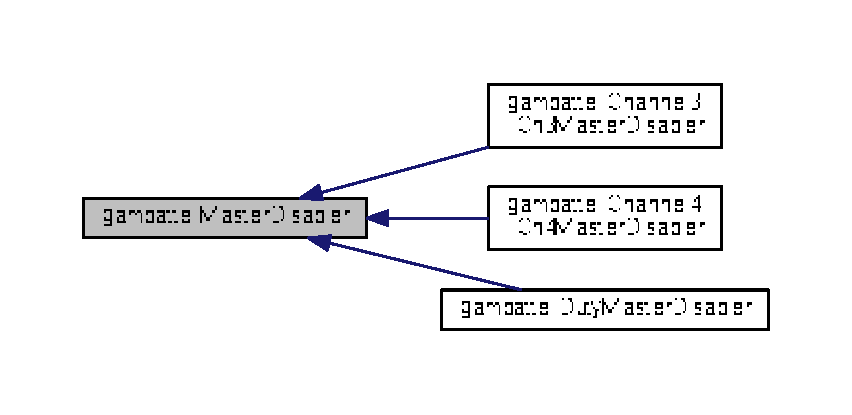
\includegraphics[width=350pt]{classgambatte_1_1MasterDisabler__inherit__graph}
\end{center}
\end{figure}
\subsection*{Public Member Functions}
\begin{DoxyCompactItemize}
\item 
\hyperlink{classgambatte_1_1MasterDisabler_ab99180b369a016f453ea9b8590821503}{Master\+Disabler} (bool \&master)
\item 
virtual \hyperlink{classgambatte_1_1MasterDisabler_ac8ac2094532c4247348557c518f68cce}{$\sim$\+Master\+Disabler} ()
\item 
virtual void \hyperlink{classgambatte_1_1MasterDisabler_a6b69f64af3e8112eac3767a74ee0e322}{operator()} ()
\end{DoxyCompactItemize}
\subsection*{Private Attributes}
\begin{DoxyCompactItemize}
\item 
bool \& \hyperlink{classgambatte_1_1MasterDisabler_ae2cb1d8720294d0f32eba06d93483a06}{master\+\_\+}
\end{DoxyCompactItemize}


\subsection{Constructor \& Destructor Documentation}
\mbox{\Hypertarget{classgambatte_1_1MasterDisabler_ab99180b369a016f453ea9b8590821503}\label{classgambatte_1_1MasterDisabler_ab99180b369a016f453ea9b8590821503}} 
\index{gambatte\+::\+Master\+Disabler@{gambatte\+::\+Master\+Disabler}!Master\+Disabler@{Master\+Disabler}}
\index{Master\+Disabler@{Master\+Disabler}!gambatte\+::\+Master\+Disabler@{gambatte\+::\+Master\+Disabler}}
\subsubsection{\texorpdfstring{Master\+Disabler()}{MasterDisabler()}}
{\footnotesize\ttfamily gambatte\+::\+Master\+Disabler\+::\+Master\+Disabler (\begin{DoxyParamCaption}\item[{bool \&}]{master }\end{DoxyParamCaption})\hspace{0.3cm}{\ttfamily [inline]}, {\ttfamily [explicit]}}

\mbox{\Hypertarget{classgambatte_1_1MasterDisabler_ac8ac2094532c4247348557c518f68cce}\label{classgambatte_1_1MasterDisabler_ac8ac2094532c4247348557c518f68cce}} 
\index{gambatte\+::\+Master\+Disabler@{gambatte\+::\+Master\+Disabler}!````~Master\+Disabler@{$\sim$\+Master\+Disabler}}
\index{````~Master\+Disabler@{$\sim$\+Master\+Disabler}!gambatte\+::\+Master\+Disabler@{gambatte\+::\+Master\+Disabler}}
\subsubsection{\texorpdfstring{$\sim$\+Master\+Disabler()}{~MasterDisabler()}}
{\footnotesize\ttfamily virtual gambatte\+::\+Master\+Disabler\+::$\sim$\+Master\+Disabler (\begin{DoxyParamCaption}{ }\end{DoxyParamCaption})\hspace{0.3cm}{\ttfamily [inline]}, {\ttfamily [virtual]}}



\subsection{Member Function Documentation}
\mbox{\Hypertarget{classgambatte_1_1MasterDisabler_a6b69f64af3e8112eac3767a74ee0e322}\label{classgambatte_1_1MasterDisabler_a6b69f64af3e8112eac3767a74ee0e322}} 
\index{gambatte\+::\+Master\+Disabler@{gambatte\+::\+Master\+Disabler}!operator()@{operator()}}
\index{operator()@{operator()}!gambatte\+::\+Master\+Disabler@{gambatte\+::\+Master\+Disabler}}
\subsubsection{\texorpdfstring{operator()()}{operator()()}}
{\footnotesize\ttfamily virtual void gambatte\+::\+Master\+Disabler\+::operator() (\begin{DoxyParamCaption}{ }\end{DoxyParamCaption})\hspace{0.3cm}{\ttfamily [inline]}, {\ttfamily [virtual]}}



Reimplemented in \hyperlink{classgambatte_1_1Channel4_1_1Ch4MasterDisabler_a7f9ddd23602b991df7ee5bb2a734cc99}{gambatte\+::\+Channel4\+::\+Ch4\+Master\+Disabler}, \hyperlink{classgambatte_1_1Channel3_1_1Ch3MasterDisabler_aa8b79b7238fc3249d6a5bb0d64aa43d1}{gambatte\+::\+Channel3\+::\+Ch3\+Master\+Disabler}, and \hyperlink{classgambatte_1_1DutyMasterDisabler_a21f513f0b20eae19255a473668a099f6}{gambatte\+::\+Duty\+Master\+Disabler}.



\subsection{Member Data Documentation}
\mbox{\Hypertarget{classgambatte_1_1MasterDisabler_ae2cb1d8720294d0f32eba06d93483a06}\label{classgambatte_1_1MasterDisabler_ae2cb1d8720294d0f32eba06d93483a06}} 
\index{gambatte\+::\+Master\+Disabler@{gambatte\+::\+Master\+Disabler}!master\+\_\+@{master\+\_\+}}
\index{master\+\_\+@{master\+\_\+}!gambatte\+::\+Master\+Disabler@{gambatte\+::\+Master\+Disabler}}
\subsubsection{\texorpdfstring{master\+\_\+}{master\_}}
{\footnotesize\ttfamily bool\& gambatte\+::\+Master\+Disabler\+::master\+\_\+\hspace{0.3cm}{\ttfamily [private]}}



The documentation for this class was generated from the following file\+:\begin{DoxyCompactItemize}
\item 
src/sound/\hyperlink{master__disabler_8h}{master\+\_\+disabler.\+h}\end{DoxyCompactItemize}

\hypertarget{classgambatte_1_1Mbc}{}\section{gambatte\+:\+:Mbc Class Reference}
\label{classgambatte_1_1Mbc}\index{gambatte\+::\+Mbc@{gambatte\+::\+Mbc}}


{\ttfamily \#include $<$cartridge.\+h$>$}

\subsection*{Public Member Functions}
\begin{DoxyCompactItemize}
\item 
virtual \hyperlink{classgambatte_1_1Mbc_a518adcdff389a3e92774e683f1af6059}{$\sim$\+Mbc} ()
\item 
virtual void \hyperlink{classgambatte_1_1Mbc_a0c05b231bad52fb08784074ddfd2e878}{rom\+Write} (unsigned P, unsigned data)=0
\item 
virtual void \hyperlink{classgambatte_1_1Mbc_a255f6aa48eb21c8b95b23d978b1f4d21}{save\+State} (\hyperlink{structgambatte_1_1SaveState_1_1Mem}{Save\+State\+::\+Mem} \&ss) const =0
\item 
virtual void \hyperlink{classgambatte_1_1Mbc_a894d6ad53d017b25a03bf45f7b910f6d}{load\+State} (\hyperlink{structgambatte_1_1SaveState_1_1Mem}{Save\+State\+::\+Mem} const \&ss)=0
\item 
virtual bool \hyperlink{classgambatte_1_1Mbc_add5e1e03b46b35d6ca593e46dba50477}{is\+Address\+Within\+Area\+Rombank\+Can\+Be\+Mapped\+To} (unsigned address, unsigned rombank) const =0
\item 
virtual void \hyperlink{classgambatte_1_1Mbc_aca51cb12ec7840299efd24e5fb5359df}{load\+Or\+Save} (\hyperlink{classgambatte_1_1loadsave}{loadsave} \&\hyperlink{ppu_8cpp_a2f2eca6997ee7baf8901725ae074d45b}{state})=0
\end{DoxyCompactItemize}


\subsection{Constructor \& Destructor Documentation}
\mbox{\Hypertarget{classgambatte_1_1Mbc_a518adcdff389a3e92774e683f1af6059}\label{classgambatte_1_1Mbc_a518adcdff389a3e92774e683f1af6059}} 
\index{gambatte\+::\+Mbc@{gambatte\+::\+Mbc}!````~Mbc@{$\sim$\+Mbc}}
\index{````~Mbc@{$\sim$\+Mbc}!gambatte\+::\+Mbc@{gambatte\+::\+Mbc}}
\subsubsection{\texorpdfstring{$\sim$\+Mbc()}{~Mbc()}}
{\footnotesize\ttfamily virtual gambatte\+::\+Mbc\+::$\sim$\+Mbc (\begin{DoxyParamCaption}{ }\end{DoxyParamCaption})\hspace{0.3cm}{\ttfamily [inline]}, {\ttfamily [virtual]}}



\subsection{Member Function Documentation}
\mbox{\Hypertarget{classgambatte_1_1Mbc_add5e1e03b46b35d6ca593e46dba50477}\label{classgambatte_1_1Mbc_add5e1e03b46b35d6ca593e46dba50477}} 
\index{gambatte\+::\+Mbc@{gambatte\+::\+Mbc}!is\+Address\+Within\+Area\+Rombank\+Can\+Be\+Mapped\+To@{is\+Address\+Within\+Area\+Rombank\+Can\+Be\+Mapped\+To}}
\index{is\+Address\+Within\+Area\+Rombank\+Can\+Be\+Mapped\+To@{is\+Address\+Within\+Area\+Rombank\+Can\+Be\+Mapped\+To}!gambatte\+::\+Mbc@{gambatte\+::\+Mbc}}
\subsubsection{\texorpdfstring{is\+Address\+Within\+Area\+Rombank\+Can\+Be\+Mapped\+To()}{isAddressWithinAreaRombankCanBeMappedTo()}}
{\footnotesize\ttfamily virtual bool gambatte\+::\+Mbc\+::is\+Address\+Within\+Area\+Rombank\+Can\+Be\+Mapped\+To (\begin{DoxyParamCaption}\item[{unsigned}]{address,  }\item[{unsigned}]{rombank }\end{DoxyParamCaption}) const\hspace{0.3cm}{\ttfamily [pure virtual]}}

\mbox{\Hypertarget{classgambatte_1_1Mbc_aca51cb12ec7840299efd24e5fb5359df}\label{classgambatte_1_1Mbc_aca51cb12ec7840299efd24e5fb5359df}} 
\index{gambatte\+::\+Mbc@{gambatte\+::\+Mbc}!load\+Or\+Save@{load\+Or\+Save}}
\index{load\+Or\+Save@{load\+Or\+Save}!gambatte\+::\+Mbc@{gambatte\+::\+Mbc}}
\subsubsection{\texorpdfstring{load\+Or\+Save()}{loadOrSave()}}
{\footnotesize\ttfamily virtual void gambatte\+::\+Mbc\+::load\+Or\+Save (\begin{DoxyParamCaption}\item[{\hyperlink{classgambatte_1_1loadsave}{loadsave} \&}]{state }\end{DoxyParamCaption})\hspace{0.3cm}{\ttfamily [pure virtual]}}

\mbox{\Hypertarget{classgambatte_1_1Mbc_a894d6ad53d017b25a03bf45f7b910f6d}\label{classgambatte_1_1Mbc_a894d6ad53d017b25a03bf45f7b910f6d}} 
\index{gambatte\+::\+Mbc@{gambatte\+::\+Mbc}!load\+State@{load\+State}}
\index{load\+State@{load\+State}!gambatte\+::\+Mbc@{gambatte\+::\+Mbc}}
\subsubsection{\texorpdfstring{load\+State()}{loadState()}}
{\footnotesize\ttfamily virtual void gambatte\+::\+Mbc\+::load\+State (\begin{DoxyParamCaption}\item[{\hyperlink{structgambatte_1_1SaveState_1_1Mem}{Save\+State\+::\+Mem} const \&}]{ss }\end{DoxyParamCaption})\hspace{0.3cm}{\ttfamily [pure virtual]}}

\mbox{\Hypertarget{classgambatte_1_1Mbc_a0c05b231bad52fb08784074ddfd2e878}\label{classgambatte_1_1Mbc_a0c05b231bad52fb08784074ddfd2e878}} 
\index{gambatte\+::\+Mbc@{gambatte\+::\+Mbc}!rom\+Write@{rom\+Write}}
\index{rom\+Write@{rom\+Write}!gambatte\+::\+Mbc@{gambatte\+::\+Mbc}}
\subsubsection{\texorpdfstring{rom\+Write()}{romWrite()}}
{\footnotesize\ttfamily virtual void gambatte\+::\+Mbc\+::rom\+Write (\begin{DoxyParamCaption}\item[{unsigned}]{P,  }\item[{unsigned}]{data }\end{DoxyParamCaption})\hspace{0.3cm}{\ttfamily [pure virtual]}}

\mbox{\Hypertarget{classgambatte_1_1Mbc_a255f6aa48eb21c8b95b23d978b1f4d21}\label{classgambatte_1_1Mbc_a255f6aa48eb21c8b95b23d978b1f4d21}} 
\index{gambatte\+::\+Mbc@{gambatte\+::\+Mbc}!save\+State@{save\+State}}
\index{save\+State@{save\+State}!gambatte\+::\+Mbc@{gambatte\+::\+Mbc}}
\subsubsection{\texorpdfstring{save\+State()}{saveState()}}
{\footnotesize\ttfamily virtual void gambatte\+::\+Mbc\+::save\+State (\begin{DoxyParamCaption}\item[{\hyperlink{structgambatte_1_1SaveState_1_1Mem}{Save\+State\+::\+Mem} \&}]{ss }\end{DoxyParamCaption}) const\hspace{0.3cm}{\ttfamily [pure virtual]}}



The documentation for this class was generated from the following file\+:\begin{DoxyCompactItemize}
\item 
src/mem/\hyperlink{cartridge_8h}{cartridge.\+h}\end{DoxyCompactItemize}

\hypertarget{structgambatte_1_1SaveState_1_1Mem}{}\section{gambatte\+:\+:Save\+State\+:\+:Mem Struct Reference}
\label{structgambatte_1_1SaveState_1_1Mem}\index{gambatte\+::\+Save\+State\+::\+Mem@{gambatte\+::\+Save\+State\+::\+Mem}}


{\ttfamily \#include $<$savestate.\+h$>$}



Collaboration diagram for gambatte\+:\+:Save\+State\+:\+:Mem\+:\nopagebreak
\begin{figure}[H]
\begin{center}
\leavevmode
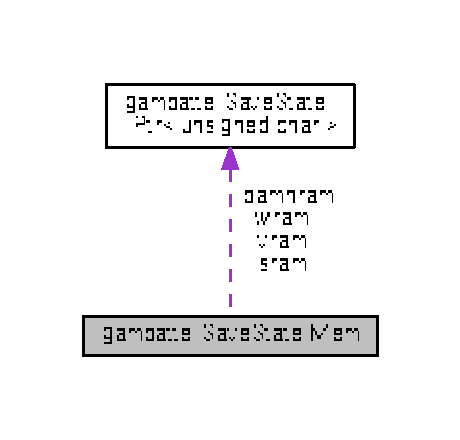
\includegraphics[width=221pt]{structgambatte_1_1SaveState_1_1Mem__coll__graph}
\end{center}
\end{figure}
\subsection*{Public Attributes}
\begin{DoxyCompactItemize}
\item 
\hyperlink{classgambatte_1_1SaveState_1_1Ptr}{Ptr}$<$ unsigned char $>$ \hyperlink{structgambatte_1_1SaveState_1_1Mem_a17be66d9d55708247cb6ea661163d433}{vram}
\item 
\hyperlink{classgambatte_1_1SaveState_1_1Ptr}{Ptr}$<$ unsigned char $>$ \hyperlink{structgambatte_1_1SaveState_1_1Mem_aa0d8ef750665ad81ec84ba8335af5800}{sram}
\item 
\hyperlink{classgambatte_1_1SaveState_1_1Ptr}{Ptr}$<$ unsigned char $>$ \hyperlink{structgambatte_1_1SaveState_1_1Mem_a61d6a15a5e1ac0253bf3a7ad26993619}{wram}
\item 
\hyperlink{classgambatte_1_1SaveState_1_1Ptr}{Ptr}$<$ unsigned char $>$ \hyperlink{structgambatte_1_1SaveState_1_1Mem_a7773fc635ffeec5c35ee65c8f2f55710}{ioamhram}
\item 
unsigned \hyperlink{structgambatte_1_1SaveState_1_1Mem_adfc72668409f448501f371c52c01d060}{div\+Last\+Update}
\item 
unsigned \hyperlink{structgambatte_1_1SaveState_1_1Mem_ac5f805a2892a39121abed21579e6a44a}{tima\+Last\+Update}
\item 
unsigned \hyperlink{structgambatte_1_1SaveState_1_1Mem_a29e42adc04bc7397724ea482ef9f14d1}{tmatime}
\item 
unsigned \hyperlink{structgambatte_1_1SaveState_1_1Mem_a53fc64a87f256305e03d64cbc9381a27}{next\+Serialtime}
\item 
unsigned \hyperlink{structgambatte_1_1SaveState_1_1Mem_a420d6b2a084c5e27c345c9b7a022c229}{last\+Oam\+Dma\+Update}
\item 
unsigned \hyperlink{structgambatte_1_1SaveState_1_1Mem_aaee943320e1021ea6b45a2286076b1fc}{min\+Int\+Time}
\item 
unsigned \hyperlink{structgambatte_1_1SaveState_1_1Mem_accd32508acb68a0119b91f27e17de6be}{unhalt\+Time}
\item 
unsigned short \hyperlink{structgambatte_1_1SaveState_1_1Mem_af1513cc3d50c10b4290221cdbe4be847}{rombank}
\item 
unsigned short \hyperlink{structgambatte_1_1SaveState_1_1Mem_a25213cf5ac03caf9500799a9804b7e77}{dma\+Source}
\item 
unsigned short \hyperlink{structgambatte_1_1SaveState_1_1Mem_ab74c2e63ce1d0eec213133583e7d55f7}{dma\+Destination}
\item 
unsigned char \hyperlink{structgambatte_1_1SaveState_1_1Mem_ac46eb550a4acc2aabef2ffe323a6cd24}{rambank}
\item 
unsigned char \hyperlink{structgambatte_1_1SaveState_1_1Mem_ad812f46789a25f4e39ae31dd0cdc1236}{oam\+Dma\+Pos}
\item 
bool \hyperlink{structgambatte_1_1SaveState_1_1Mem_af09eedb50f5dd691378612fd20fa4b39}{I\+ME}
\item 
bool \hyperlink{structgambatte_1_1SaveState_1_1Mem_a28cc6ab288d5c84e3c4140e3a72f742d}{halted}
\item 
bool \hyperlink{structgambatte_1_1SaveState_1_1Mem_a7f01ccf9678dc61ca5b1db4e3733e6c6}{enable\+Ram}
\item 
bool \hyperlink{structgambatte_1_1SaveState_1_1Mem_adee0625c6943456a851d73eb3aed4245}{rambank\+Mode}
\item 
bool \hyperlink{structgambatte_1_1SaveState_1_1Mem_a888b5a886f68c63ddb78ec2c1b95b343}{hdma\+Transfer}
\end{DoxyCompactItemize}


\subsection{Member Data Documentation}
\mbox{\Hypertarget{structgambatte_1_1SaveState_1_1Mem_adfc72668409f448501f371c52c01d060}\label{structgambatte_1_1SaveState_1_1Mem_adfc72668409f448501f371c52c01d060}} 
\index{gambatte\+::\+Save\+State\+::\+Mem@{gambatte\+::\+Save\+State\+::\+Mem}!div\+Last\+Update@{div\+Last\+Update}}
\index{div\+Last\+Update@{div\+Last\+Update}!gambatte\+::\+Save\+State\+::\+Mem@{gambatte\+::\+Save\+State\+::\+Mem}}
\subsubsection{\texorpdfstring{div\+Last\+Update}{divLastUpdate}}
{\footnotesize\ttfamily unsigned gambatte\+::\+Save\+State\+::\+Mem\+::div\+Last\+Update}

\mbox{\Hypertarget{structgambatte_1_1SaveState_1_1Mem_ab74c2e63ce1d0eec213133583e7d55f7}\label{structgambatte_1_1SaveState_1_1Mem_ab74c2e63ce1d0eec213133583e7d55f7}} 
\index{gambatte\+::\+Save\+State\+::\+Mem@{gambatte\+::\+Save\+State\+::\+Mem}!dma\+Destination@{dma\+Destination}}
\index{dma\+Destination@{dma\+Destination}!gambatte\+::\+Save\+State\+::\+Mem@{gambatte\+::\+Save\+State\+::\+Mem}}
\subsubsection{\texorpdfstring{dma\+Destination}{dmaDestination}}
{\footnotesize\ttfamily unsigned short gambatte\+::\+Save\+State\+::\+Mem\+::dma\+Destination}

\mbox{\Hypertarget{structgambatte_1_1SaveState_1_1Mem_a25213cf5ac03caf9500799a9804b7e77}\label{structgambatte_1_1SaveState_1_1Mem_a25213cf5ac03caf9500799a9804b7e77}} 
\index{gambatte\+::\+Save\+State\+::\+Mem@{gambatte\+::\+Save\+State\+::\+Mem}!dma\+Source@{dma\+Source}}
\index{dma\+Source@{dma\+Source}!gambatte\+::\+Save\+State\+::\+Mem@{gambatte\+::\+Save\+State\+::\+Mem}}
\subsubsection{\texorpdfstring{dma\+Source}{dmaSource}}
{\footnotesize\ttfamily unsigned short gambatte\+::\+Save\+State\+::\+Mem\+::dma\+Source}

\mbox{\Hypertarget{structgambatte_1_1SaveState_1_1Mem_a7f01ccf9678dc61ca5b1db4e3733e6c6}\label{structgambatte_1_1SaveState_1_1Mem_a7f01ccf9678dc61ca5b1db4e3733e6c6}} 
\index{gambatte\+::\+Save\+State\+::\+Mem@{gambatte\+::\+Save\+State\+::\+Mem}!enable\+Ram@{enable\+Ram}}
\index{enable\+Ram@{enable\+Ram}!gambatte\+::\+Save\+State\+::\+Mem@{gambatte\+::\+Save\+State\+::\+Mem}}
\subsubsection{\texorpdfstring{enable\+Ram}{enableRam}}
{\footnotesize\ttfamily bool gambatte\+::\+Save\+State\+::\+Mem\+::enable\+Ram}

\mbox{\Hypertarget{structgambatte_1_1SaveState_1_1Mem_a28cc6ab288d5c84e3c4140e3a72f742d}\label{structgambatte_1_1SaveState_1_1Mem_a28cc6ab288d5c84e3c4140e3a72f742d}} 
\index{gambatte\+::\+Save\+State\+::\+Mem@{gambatte\+::\+Save\+State\+::\+Mem}!halted@{halted}}
\index{halted@{halted}!gambatte\+::\+Save\+State\+::\+Mem@{gambatte\+::\+Save\+State\+::\+Mem}}
\subsubsection{\texorpdfstring{halted}{halted}}
{\footnotesize\ttfamily bool gambatte\+::\+Save\+State\+::\+Mem\+::halted}

\mbox{\Hypertarget{structgambatte_1_1SaveState_1_1Mem_a888b5a886f68c63ddb78ec2c1b95b343}\label{structgambatte_1_1SaveState_1_1Mem_a888b5a886f68c63ddb78ec2c1b95b343}} 
\index{gambatte\+::\+Save\+State\+::\+Mem@{gambatte\+::\+Save\+State\+::\+Mem}!hdma\+Transfer@{hdma\+Transfer}}
\index{hdma\+Transfer@{hdma\+Transfer}!gambatte\+::\+Save\+State\+::\+Mem@{gambatte\+::\+Save\+State\+::\+Mem}}
\subsubsection{\texorpdfstring{hdma\+Transfer}{hdmaTransfer}}
{\footnotesize\ttfamily bool gambatte\+::\+Save\+State\+::\+Mem\+::hdma\+Transfer}

\mbox{\Hypertarget{structgambatte_1_1SaveState_1_1Mem_af09eedb50f5dd691378612fd20fa4b39}\label{structgambatte_1_1SaveState_1_1Mem_af09eedb50f5dd691378612fd20fa4b39}} 
\index{gambatte\+::\+Save\+State\+::\+Mem@{gambatte\+::\+Save\+State\+::\+Mem}!I\+ME@{I\+ME}}
\index{I\+ME@{I\+ME}!gambatte\+::\+Save\+State\+::\+Mem@{gambatte\+::\+Save\+State\+::\+Mem}}
\subsubsection{\texorpdfstring{I\+ME}{IME}}
{\footnotesize\ttfamily bool gambatte\+::\+Save\+State\+::\+Mem\+::\+I\+ME}

\mbox{\Hypertarget{structgambatte_1_1SaveState_1_1Mem_a7773fc635ffeec5c35ee65c8f2f55710}\label{structgambatte_1_1SaveState_1_1Mem_a7773fc635ffeec5c35ee65c8f2f55710}} 
\index{gambatte\+::\+Save\+State\+::\+Mem@{gambatte\+::\+Save\+State\+::\+Mem}!ioamhram@{ioamhram}}
\index{ioamhram@{ioamhram}!gambatte\+::\+Save\+State\+::\+Mem@{gambatte\+::\+Save\+State\+::\+Mem}}
\subsubsection{\texorpdfstring{ioamhram}{ioamhram}}
{\footnotesize\ttfamily \hyperlink{classgambatte_1_1SaveState_1_1Ptr}{Ptr}$<$unsigned char$>$ gambatte\+::\+Save\+State\+::\+Mem\+::ioamhram}

\mbox{\Hypertarget{structgambatte_1_1SaveState_1_1Mem_a420d6b2a084c5e27c345c9b7a022c229}\label{structgambatte_1_1SaveState_1_1Mem_a420d6b2a084c5e27c345c9b7a022c229}} 
\index{gambatte\+::\+Save\+State\+::\+Mem@{gambatte\+::\+Save\+State\+::\+Mem}!last\+Oam\+Dma\+Update@{last\+Oam\+Dma\+Update}}
\index{last\+Oam\+Dma\+Update@{last\+Oam\+Dma\+Update}!gambatte\+::\+Save\+State\+::\+Mem@{gambatte\+::\+Save\+State\+::\+Mem}}
\subsubsection{\texorpdfstring{last\+Oam\+Dma\+Update}{lastOamDmaUpdate}}
{\footnotesize\ttfamily unsigned gambatte\+::\+Save\+State\+::\+Mem\+::last\+Oam\+Dma\+Update}

\mbox{\Hypertarget{structgambatte_1_1SaveState_1_1Mem_aaee943320e1021ea6b45a2286076b1fc}\label{structgambatte_1_1SaveState_1_1Mem_aaee943320e1021ea6b45a2286076b1fc}} 
\index{gambatte\+::\+Save\+State\+::\+Mem@{gambatte\+::\+Save\+State\+::\+Mem}!min\+Int\+Time@{min\+Int\+Time}}
\index{min\+Int\+Time@{min\+Int\+Time}!gambatte\+::\+Save\+State\+::\+Mem@{gambatte\+::\+Save\+State\+::\+Mem}}
\subsubsection{\texorpdfstring{min\+Int\+Time}{minIntTime}}
{\footnotesize\ttfamily unsigned gambatte\+::\+Save\+State\+::\+Mem\+::min\+Int\+Time}

\mbox{\Hypertarget{structgambatte_1_1SaveState_1_1Mem_a53fc64a87f256305e03d64cbc9381a27}\label{structgambatte_1_1SaveState_1_1Mem_a53fc64a87f256305e03d64cbc9381a27}} 
\index{gambatte\+::\+Save\+State\+::\+Mem@{gambatte\+::\+Save\+State\+::\+Mem}!next\+Serialtime@{next\+Serialtime}}
\index{next\+Serialtime@{next\+Serialtime}!gambatte\+::\+Save\+State\+::\+Mem@{gambatte\+::\+Save\+State\+::\+Mem}}
\subsubsection{\texorpdfstring{next\+Serialtime}{nextSerialtime}}
{\footnotesize\ttfamily unsigned gambatte\+::\+Save\+State\+::\+Mem\+::next\+Serialtime}

\mbox{\Hypertarget{structgambatte_1_1SaveState_1_1Mem_ad812f46789a25f4e39ae31dd0cdc1236}\label{structgambatte_1_1SaveState_1_1Mem_ad812f46789a25f4e39ae31dd0cdc1236}} 
\index{gambatte\+::\+Save\+State\+::\+Mem@{gambatte\+::\+Save\+State\+::\+Mem}!oam\+Dma\+Pos@{oam\+Dma\+Pos}}
\index{oam\+Dma\+Pos@{oam\+Dma\+Pos}!gambatte\+::\+Save\+State\+::\+Mem@{gambatte\+::\+Save\+State\+::\+Mem}}
\subsubsection{\texorpdfstring{oam\+Dma\+Pos}{oamDmaPos}}
{\footnotesize\ttfamily unsigned char gambatte\+::\+Save\+State\+::\+Mem\+::oam\+Dma\+Pos}

\mbox{\Hypertarget{structgambatte_1_1SaveState_1_1Mem_ac46eb550a4acc2aabef2ffe323a6cd24}\label{structgambatte_1_1SaveState_1_1Mem_ac46eb550a4acc2aabef2ffe323a6cd24}} 
\index{gambatte\+::\+Save\+State\+::\+Mem@{gambatte\+::\+Save\+State\+::\+Mem}!rambank@{rambank}}
\index{rambank@{rambank}!gambatte\+::\+Save\+State\+::\+Mem@{gambatte\+::\+Save\+State\+::\+Mem}}
\subsubsection{\texorpdfstring{rambank}{rambank}}
{\footnotesize\ttfamily unsigned char gambatte\+::\+Save\+State\+::\+Mem\+::rambank}

\mbox{\Hypertarget{structgambatte_1_1SaveState_1_1Mem_adee0625c6943456a851d73eb3aed4245}\label{structgambatte_1_1SaveState_1_1Mem_adee0625c6943456a851d73eb3aed4245}} 
\index{gambatte\+::\+Save\+State\+::\+Mem@{gambatte\+::\+Save\+State\+::\+Mem}!rambank\+Mode@{rambank\+Mode}}
\index{rambank\+Mode@{rambank\+Mode}!gambatte\+::\+Save\+State\+::\+Mem@{gambatte\+::\+Save\+State\+::\+Mem}}
\subsubsection{\texorpdfstring{rambank\+Mode}{rambankMode}}
{\footnotesize\ttfamily bool gambatte\+::\+Save\+State\+::\+Mem\+::rambank\+Mode}

\mbox{\Hypertarget{structgambatte_1_1SaveState_1_1Mem_af1513cc3d50c10b4290221cdbe4be847}\label{structgambatte_1_1SaveState_1_1Mem_af1513cc3d50c10b4290221cdbe4be847}} 
\index{gambatte\+::\+Save\+State\+::\+Mem@{gambatte\+::\+Save\+State\+::\+Mem}!rombank@{rombank}}
\index{rombank@{rombank}!gambatte\+::\+Save\+State\+::\+Mem@{gambatte\+::\+Save\+State\+::\+Mem}}
\subsubsection{\texorpdfstring{rombank}{rombank}}
{\footnotesize\ttfamily unsigned short gambatte\+::\+Save\+State\+::\+Mem\+::rombank}

\mbox{\Hypertarget{structgambatte_1_1SaveState_1_1Mem_aa0d8ef750665ad81ec84ba8335af5800}\label{structgambatte_1_1SaveState_1_1Mem_aa0d8ef750665ad81ec84ba8335af5800}} 
\index{gambatte\+::\+Save\+State\+::\+Mem@{gambatte\+::\+Save\+State\+::\+Mem}!sram@{sram}}
\index{sram@{sram}!gambatte\+::\+Save\+State\+::\+Mem@{gambatte\+::\+Save\+State\+::\+Mem}}
\subsubsection{\texorpdfstring{sram}{sram}}
{\footnotesize\ttfamily \hyperlink{classgambatte_1_1SaveState_1_1Ptr}{Ptr}$<$unsigned char$>$ gambatte\+::\+Save\+State\+::\+Mem\+::sram}

\mbox{\Hypertarget{structgambatte_1_1SaveState_1_1Mem_ac5f805a2892a39121abed21579e6a44a}\label{structgambatte_1_1SaveState_1_1Mem_ac5f805a2892a39121abed21579e6a44a}} 
\index{gambatte\+::\+Save\+State\+::\+Mem@{gambatte\+::\+Save\+State\+::\+Mem}!tima\+Last\+Update@{tima\+Last\+Update}}
\index{tima\+Last\+Update@{tima\+Last\+Update}!gambatte\+::\+Save\+State\+::\+Mem@{gambatte\+::\+Save\+State\+::\+Mem}}
\subsubsection{\texorpdfstring{tima\+Last\+Update}{timaLastUpdate}}
{\footnotesize\ttfamily unsigned gambatte\+::\+Save\+State\+::\+Mem\+::tima\+Last\+Update}

\mbox{\Hypertarget{structgambatte_1_1SaveState_1_1Mem_a29e42adc04bc7397724ea482ef9f14d1}\label{structgambatte_1_1SaveState_1_1Mem_a29e42adc04bc7397724ea482ef9f14d1}} 
\index{gambatte\+::\+Save\+State\+::\+Mem@{gambatte\+::\+Save\+State\+::\+Mem}!tmatime@{tmatime}}
\index{tmatime@{tmatime}!gambatte\+::\+Save\+State\+::\+Mem@{gambatte\+::\+Save\+State\+::\+Mem}}
\subsubsection{\texorpdfstring{tmatime}{tmatime}}
{\footnotesize\ttfamily unsigned gambatte\+::\+Save\+State\+::\+Mem\+::tmatime}

\mbox{\Hypertarget{structgambatte_1_1SaveState_1_1Mem_accd32508acb68a0119b91f27e17de6be}\label{structgambatte_1_1SaveState_1_1Mem_accd32508acb68a0119b91f27e17de6be}} 
\index{gambatte\+::\+Save\+State\+::\+Mem@{gambatte\+::\+Save\+State\+::\+Mem}!unhalt\+Time@{unhalt\+Time}}
\index{unhalt\+Time@{unhalt\+Time}!gambatte\+::\+Save\+State\+::\+Mem@{gambatte\+::\+Save\+State\+::\+Mem}}
\subsubsection{\texorpdfstring{unhalt\+Time}{unhaltTime}}
{\footnotesize\ttfamily unsigned gambatte\+::\+Save\+State\+::\+Mem\+::unhalt\+Time}

\mbox{\Hypertarget{structgambatte_1_1SaveState_1_1Mem_a17be66d9d55708247cb6ea661163d433}\label{structgambatte_1_1SaveState_1_1Mem_a17be66d9d55708247cb6ea661163d433}} 
\index{gambatte\+::\+Save\+State\+::\+Mem@{gambatte\+::\+Save\+State\+::\+Mem}!vram@{vram}}
\index{vram@{vram}!gambatte\+::\+Save\+State\+::\+Mem@{gambatte\+::\+Save\+State\+::\+Mem}}
\subsubsection{\texorpdfstring{vram}{vram}}
{\footnotesize\ttfamily \hyperlink{classgambatte_1_1SaveState_1_1Ptr}{Ptr}$<$unsigned char$>$ gambatte\+::\+Save\+State\+::\+Mem\+::vram}

\mbox{\Hypertarget{structgambatte_1_1SaveState_1_1Mem_a61d6a15a5e1ac0253bf3a7ad26993619}\label{structgambatte_1_1SaveState_1_1Mem_a61d6a15a5e1ac0253bf3a7ad26993619}} 
\index{gambatte\+::\+Save\+State\+::\+Mem@{gambatte\+::\+Save\+State\+::\+Mem}!wram@{wram}}
\index{wram@{wram}!gambatte\+::\+Save\+State\+::\+Mem@{gambatte\+::\+Save\+State\+::\+Mem}}
\subsubsection{\texorpdfstring{wram}{wram}}
{\footnotesize\ttfamily \hyperlink{classgambatte_1_1SaveState_1_1Ptr}{Ptr}$<$unsigned char$>$ gambatte\+::\+Save\+State\+::\+Mem\+::wram}



The documentation for this struct was generated from the following file\+:\begin{DoxyCompactItemize}
\item 
src/\hyperlink{savestate_8h}{savestate.\+h}\end{DoxyCompactItemize}

\hypertarget{classgambatte_1_1Memory}{}\section{gambatte\+:\+:Memory Class Reference}
\label{classgambatte_1_1Memory}\index{gambatte\+::\+Memory@{gambatte\+::\+Memory}}


{\ttfamily \#include $<$memory.\+h$>$}



Collaboration diagram for gambatte\+:\+:Memory\+:
\nopagebreak
\begin{figure}[H]
\begin{center}
\leavevmode
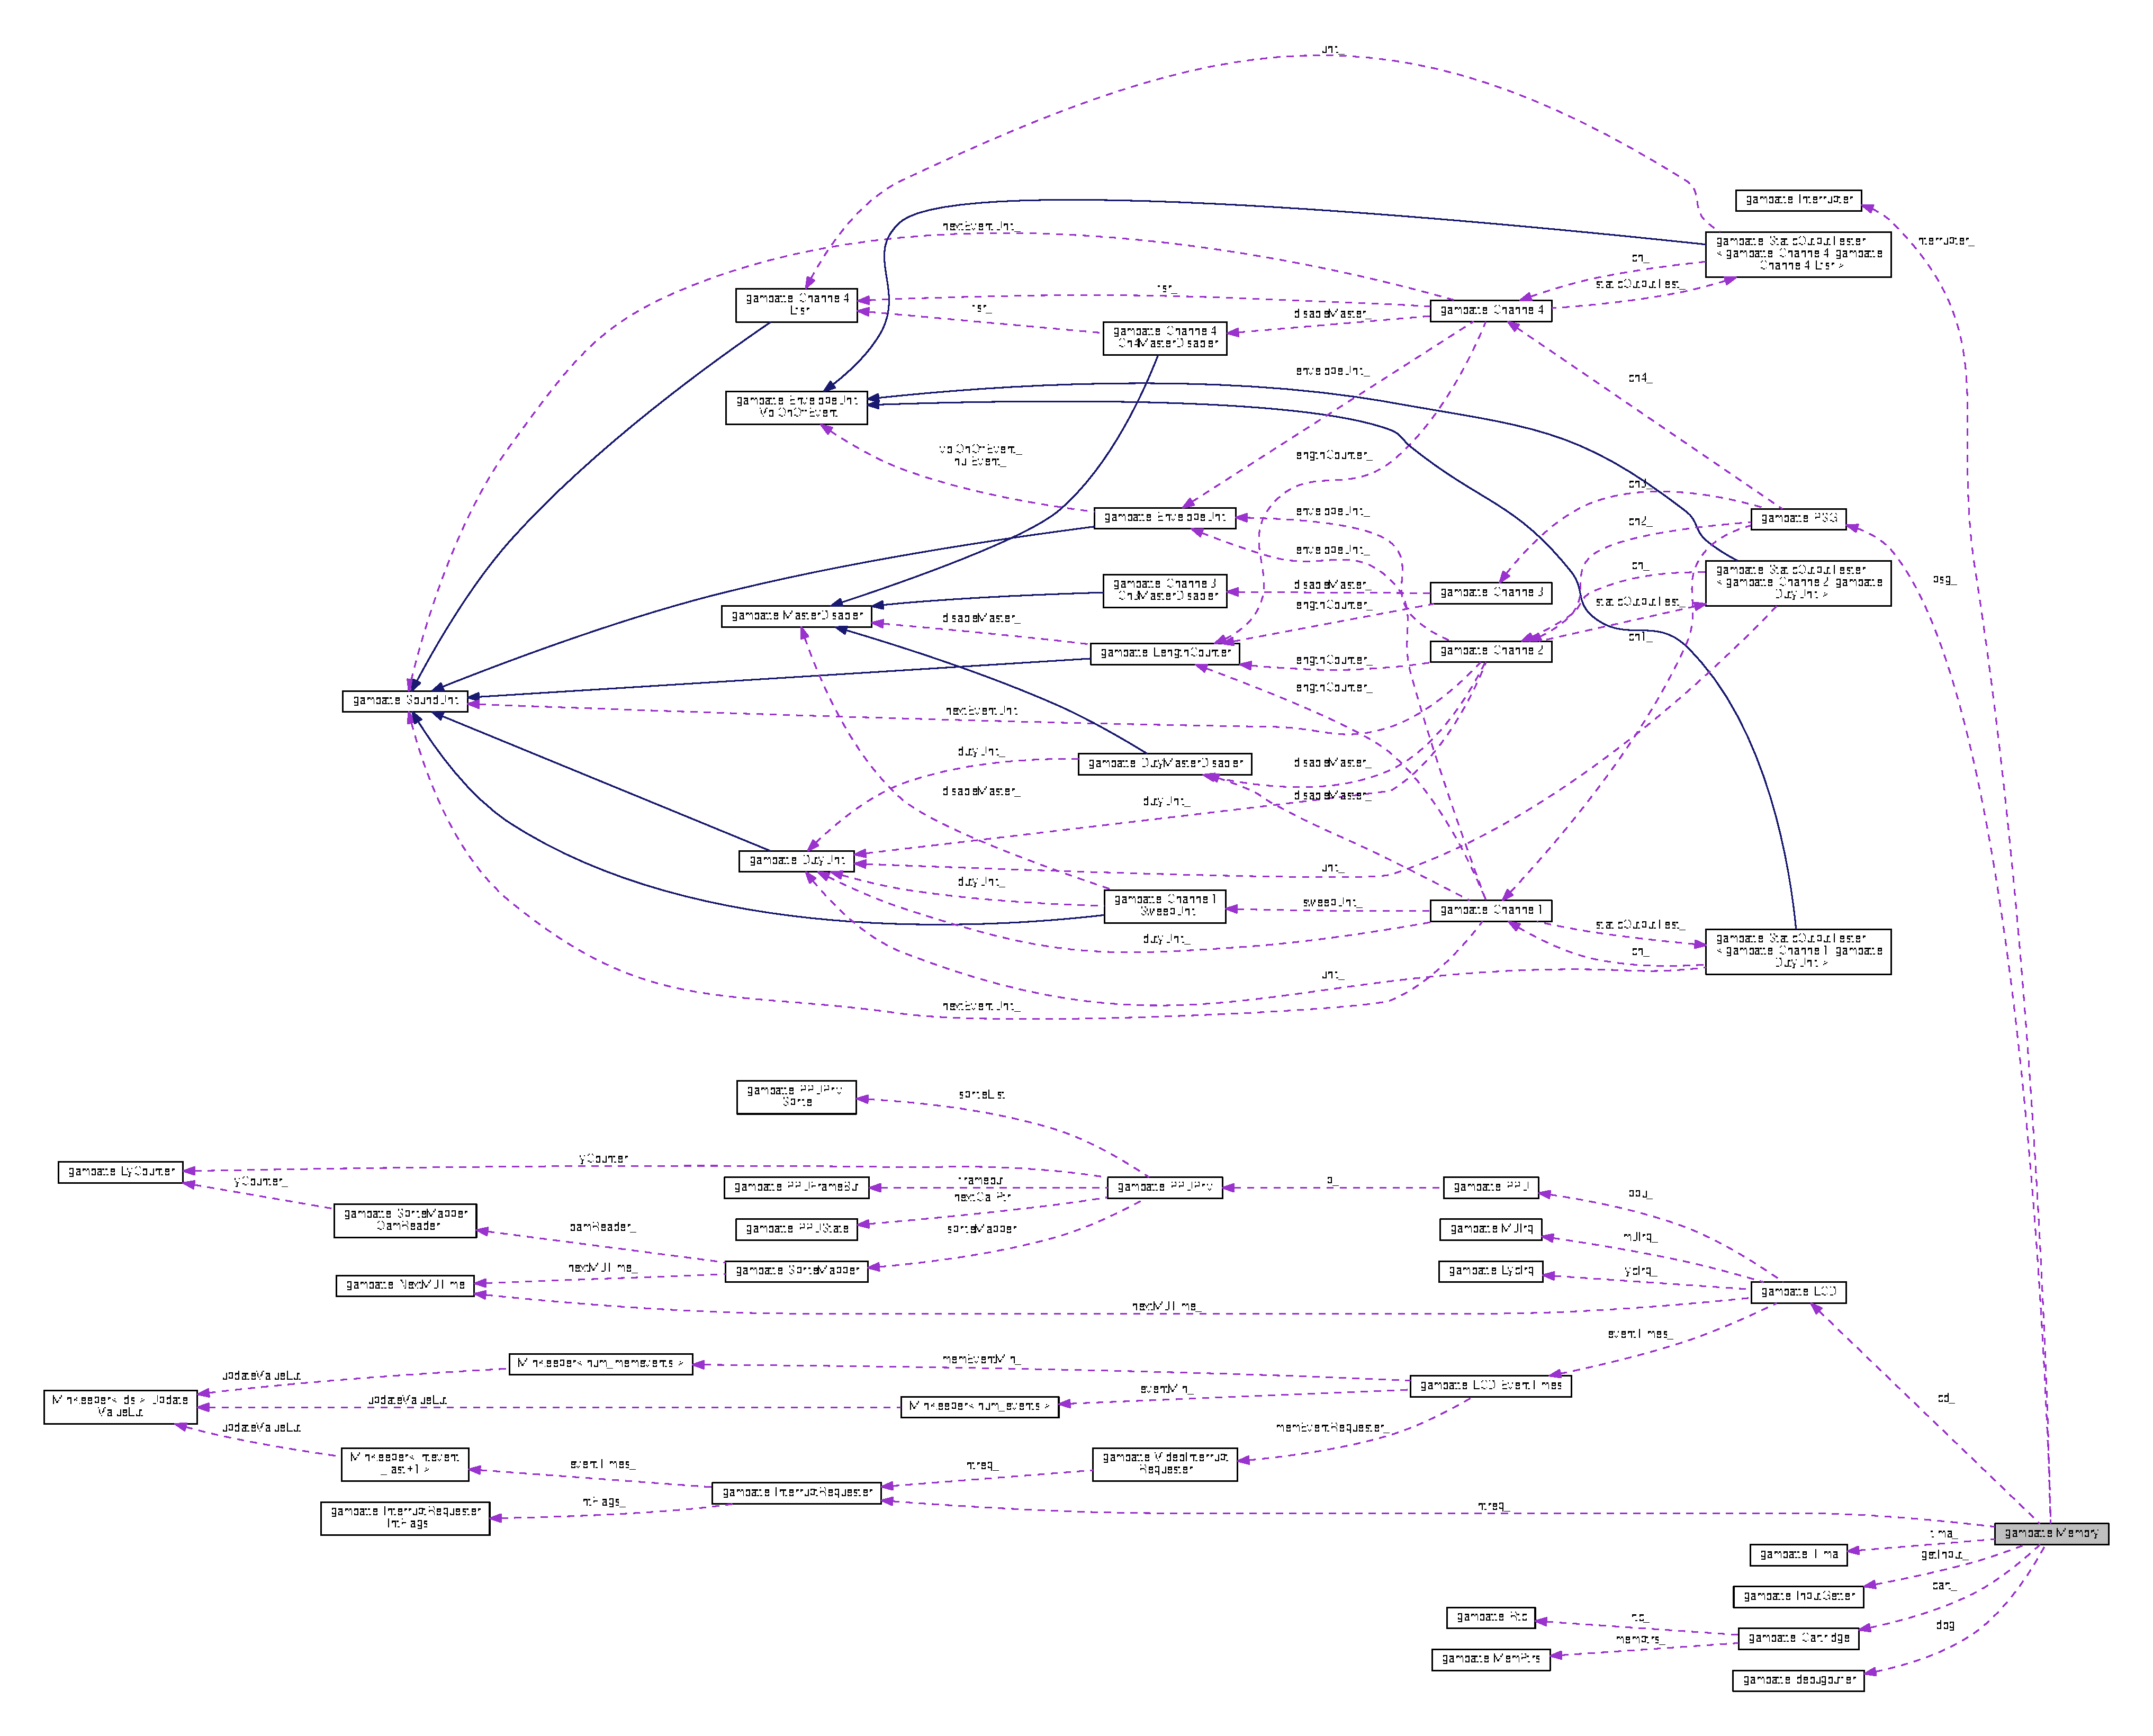
\includegraphics[width=350pt]{classgambatte_1_1Memory__coll__graph}
\end{center}
\end{figure}
\subsection*{Public Member Functions}
\begin{DoxyCompactItemize}
\item 
\hyperlink{classgambatte_1_1Memory_a9945124a92611e7868bbd52418a3e40c}{Memory} (\hyperlink{classgambatte_1_1Interrupter}{Interrupter} const \&interrupter, time\+\_\+t($\ast$$\ast$gettime)())
\item 
bool \hyperlink{classgambatte_1_1Memory_ac408f41b5da4d1dcf78b13bf4658f9e8}{loaded} () const
\item 
char const  $\ast$ \hyperlink{classgambatte_1_1Memory_a6a1305328c8499d094f17339871d560c}{rom\+Title} () const
\item 
\hyperlink{classgambatte_1_1PakInfo}{Pak\+Info} const \hyperlink{classgambatte_1_1Memory_a0777592e6bd7ae61aa89d6d4335d6970}{pak\+Info} (bool multicart\+Compat) const
\item 
void \hyperlink{classgambatte_1_1Memory_a1e277e1f1b72165fb334139471fc8418}{set\+State\+Ptrs} (\hyperlink{structgambatte_1_1SaveState}{Save\+State} \&\hyperlink{ppu_8cpp_a2f2eca6997ee7baf8901725ae074d45b}{state})
\item 
unsigned \hyperlink{classgambatte_1_1Memory_a1dc38f529eb812d8720ea02d0f4ae6fe}{save\+State} (\hyperlink{structgambatte_1_1SaveState}{Save\+State} \&\hyperlink{ppu_8cpp_a2f2eca6997ee7baf8901725ae074d45b}{state}, unsigned cc)
\item 
void \hyperlink{classgambatte_1_1Memory_a40b7846d15c6e94c925e996ee49d23e7}{load\+Or\+Save} (\hyperlink{classgambatte_1_1loadsave}{loadsave} \&\hyperlink{ppu_8cpp_a2f2eca6997ee7baf8901725ae074d45b}{state})
\item 
void \hyperlink{classgambatte_1_1Memory_acbee7abfbfc1db12aac70effcee425e5}{load\+State} (\hyperlink{structgambatte_1_1SaveState}{Save\+State} const \&\hyperlink{ppu_8cpp_a2f2eca6997ee7baf8901725ae074d45b}{state})
\item 
void \hyperlink{classgambatte_1_1Memory_a48044eb49376c2cd2a71eaacef835c24}{load\+Savedata} ()
\item 
void \hyperlink{classgambatte_1_1Memory_a1712a9407525b2de710b055106b5770c}{save\+Savedata} ()
\item 
std\+::string const \hyperlink{classgambatte_1_1Memory_a83a8f1281b2dd704eaffb7dc6222948d}{save\+Base\+Path} () const
\item 
void \hyperlink{classgambatte_1_1Memory_a86d9fc1ad5d5b350dd32605f81fb4a4a}{set\+Osd\+Element} (transfer\+\_\+ptr$<$ \hyperlink{classgambatte_1_1OsdElement}{Osd\+Element} $>$ osd\+Element)
\item 
unsigned \hyperlink{classgambatte_1_1Memory_a8db40205a514b6c1c916c81221152f35}{stop} (unsigned cycle\+Counter)
\item 
bool \hyperlink{classgambatte_1_1Memory_a9ef6331153d37826ff61a5e568013d5d}{is\+Cgb} () const
\item 
bool \hyperlink{classgambatte_1_1Memory_a98508701538fe2c57b835af55d38c4f7}{ime} () const
\item 
bool \hyperlink{classgambatte_1_1Memory_a5026aed969d2b61931cee0ca83198738}{halted} () const
\item 
unsigned \hyperlink{classgambatte_1_1Memory_a42fa8551b61a4a821f8b13ee9c2f235c}{next\+Event\+Time} () const
\item 
bool \hyperlink{classgambatte_1_1Memory_ac1124fabe601d7249d3677686edfdf3d}{is\+Active} () const
\item 
signed \hyperlink{classgambatte_1_1Memory_a8cdf9d89d7c6fd3acba8ba0e83b09044}{cycles\+Since\+Blit} (unsigned cc) const
\item 
void \hyperlink{classgambatte_1_1Memory_a4a32fa3e44e16368c4a224cb553fa1a3}{halt} ()
\item 
void \hyperlink{classgambatte_1_1Memory_a71209c5ac16a9616891af00f252ed8ff}{ei} (unsigned cycle\+Counter)
\item 
void \hyperlink{classgambatte_1_1Memory_a6ffc8cfb0c4dbd5ca3f92c4c7bbda0a4}{di} ()
\item 
void \hyperlink{classgambatte_1_1Memory_aa2cbd6ac6d07a09b6a2049899e5ab5d0}{set\+\_\+debug\+\_\+buffer} (\hyperlink{structgambatte_1_1debugbuffer}{debugbuffer} \&dbgbuf)
\item 
unsigned \hyperlink{classgambatte_1_1Memory_a2b2660fe50e46ec79c445e55ef3973a5}{ff\+\_\+read} (unsigned p, unsigned cc)
\item 
uint8\+\_\+t \hyperlink{classgambatte_1_1Memory_a35243d758e0bd8bc6b33162a58384d5b}{do\+\_\+read\+\_\+trap} (const uint8\+\_\+t $\ast$addr, std\+::pair$<$ unsigned char $\ast$, size\+\_\+t $>$ area, unsigned clazz, const uint8\+\_\+t $\ast$dbgflags, std\+::map$<$ unsigned, uint8\+\_\+t $>$ \&cheats, uint8\+\_\+t v, uint8\+\_\+t mask, bool exec)
\item 
void \hyperlink{classgambatte_1_1Memory_a8fe0102b1325cd50a8cb133a02ceb77e}{do\+\_\+write\+\_\+trap} (const uint8\+\_\+t $\ast$addr, std\+::pair$<$ unsigned char $\ast$, size\+\_\+t $>$ area, unsigned clazz, const uint8\+\_\+t $\ast$dbgflags, uint8\+\_\+t v)
\item 
unsigned \hyperlink{classgambatte_1_1Memory_a6c94da014e7e90d1aefc92064df0b949}{read} (unsigned p, unsigned cc, bool exec)
\item 
void \hyperlink{classgambatte_1_1Memory_ab3d9319beaaaac71d849d26753cb77db}{write} (unsigned p, unsigned data, unsigned cc)
\item 
void \hyperlink{classgambatte_1_1Memory_a8afeda5a0509bd8e44858aef7cf5d2c0}{ff\+\_\+write} (unsigned p, unsigned data, unsigned cc)
\item 
\hyperlink{namespacegambatte_a42606f494711d2e2870a5f5cdf69e468}{Load\+Res} \hyperlink{classgambatte_1_1Memory_a3bdc9bdbc6385c8c35817cfe1c7bc9f7}{load\+R\+OM} (const std\+::string \&romfile, bool force\+Dmg, bool multicart\+Compat)
\item 
\hyperlink{namespacegambatte_a42606f494711d2e2870a5f5cdf69e468}{Load\+Res} \hyperlink{classgambatte_1_1Memory_adb1cd8bdc21ebc61b0a7c168aa6f9bf0}{load\+R\+OM} (const unsigned char $\ast$image, size\+\_\+t isize, bool force\+Dmg, bool multicart\+Compat)
\item 
void \hyperlink{classgambatte_1_1Memory_a848742d4e0fcfa3a6bc47cccc5f3f40a}{set\+Video\+Buffer} (\hyperlink{namespacegambatte_a0639f09fccfbbd5a8e0796318768e370}{uint\+\_\+least32\+\_\+t} $\ast$const video\+Buf, std\+::ptrdiff\+\_\+t pitch)
\item 
void \hyperlink{classgambatte_1_1Memory_a6ab73e62b7f606e2eaca2b14126f323d}{set\+Rtc\+Base} (time\+\_\+t time)
\item 
time\+\_\+t \hyperlink{classgambatte_1_1Memory_a2ba8f652872f268e9c954782533c4e55}{get\+Rtc\+Base} ()
\item 
std\+::pair$<$ unsigned char $\ast$, size\+\_\+t $>$ \hyperlink{classgambatte_1_1Memory_a26a6cdbc6488edc53271fe4315cc98a9}{get\+Work\+Ram} ()
\item 
std\+::pair$<$ unsigned char $\ast$, size\+\_\+t $>$ \hyperlink{classgambatte_1_1Memory_a05665cbf3eab8aa166ace880f337c05b}{get\+Save\+Ram} ()
\item 
std\+::pair$<$ unsigned char $\ast$, size\+\_\+t $>$ \hyperlink{classgambatte_1_1Memory_a12c2cd723ca7d0e263a50381c46cbd74}{get\+Io\+Ram} ()
\item 
std\+::pair$<$ unsigned char $\ast$, size\+\_\+t $>$ \hyperlink{classgambatte_1_1Memory_ad663efd3d0942cdb217eeb5e41532443}{get\+Video\+Ram} ()
\item 
unsigned \hyperlink{classgambatte_1_1Memory_ad5bda65c2e16fb12d8caf402aa851211}{event} (unsigned cycle\+Counter)
\item 
unsigned \hyperlink{classgambatte_1_1Memory_a3a881c3c7934b52ca94045f02d8eaf65}{reset\+Counters} (unsigned cycle\+Counter)
\item 
void \hyperlink{classgambatte_1_1Memory_a7714bc6dde09f9799cc47eff78c5af9a}{set\+Save\+Dir} (std\+::string const \&dir)
\item 
void \hyperlink{classgambatte_1_1Memory_a3a009a30b0e9d3d32577eee2380f9d45}{set\+Input\+Getter} (\hyperlink{classgambatte_1_1InputGetter}{Input\+Getter} $\ast$get\+Input)
\item 
void \hyperlink{classgambatte_1_1Memory_abfacd022d4954e43a1a5417cfa6df64f}{set\+Endtime} (unsigned cc, unsigned inc)
\item 
void \hyperlink{classgambatte_1_1Memory_ae2308d0ffae1dd433a208ba656239f6b}{set\+Sound\+Buffer} (\hyperlink{namespacegambatte_a0639f09fccfbbd5a8e0796318768e370}{uint\+\_\+least32\+\_\+t} $\ast$\hyperlink{ioapi_8h_a8ad8a13c88886b9f623034ff88570adb}{buf})
\item 
unsigned \hyperlink{classgambatte_1_1Memory_a61edfc3d2a539c12e59c7ad4753a5d8a}{fill\+Sound\+Buffer} (unsigned cc)
\item 
void \hyperlink{classgambatte_1_1Memory_a59d17e56fc8dd57a2862d4ddfe6e9547}{set\+Dmg\+Palette\+Color} (unsigned pal\+Num, unsigned color\+Num, \hyperlink{namespacegambatte_a0639f09fccfbbd5a8e0796318768e370}{uint\+\_\+least32\+\_\+t} rgb32)
\item 
void \hyperlink{classgambatte_1_1Memory_a842ec84c708a183b3fba3de7bddfa574}{set\+Game\+Genie} (std\+::string const \&codes)
\item 
void \hyperlink{classgambatte_1_1Memory_a8a5f8551b35968c8e80f9f3cae06ffaf}{set\+Game\+Shark} (std\+::string const \&codes)
\item 
\hyperlink{structgambatte_1_1debugbuffer}{debugbuffer} $\ast$ \hyperlink{classgambatte_1_1Memory_a12d63c99f789ae6a33c60abd2192d4e3}{get\+\_\+debug} ()
\item 
void \hyperlink{classgambatte_1_1Memory_aa4e82534365704f7226fa0d4ee61df33}{print\+\_\+interrupt\+\_\+timing} (void)
\end{DoxyCompactItemize}
\subsection*{Private Member Functions}
\begin{DoxyCompactItemize}
\item 
void \hyperlink{classgambatte_1_1Memory_a95b92fe66c06b9694ed31c8535a0479c}{update\+Input} ()
\item 
void \hyperlink{classgambatte_1_1Memory_a2ea1cb0bdcc6e3e7124be5a938a57ac6}{dec\+Event\+Cycles} (\hyperlink{namespacegambatte_a0cc3dd7d4d26f0466e9eeda6242755d9}{Int\+Event\+Id} event\+Id, unsigned dec)
\item 
void \hyperlink{classgambatte_1_1Memory_af092fa032a019af9a7af862483439cac}{oam\+Dma\+Init\+Setup} ()
\item 
void \hyperlink{classgambatte_1_1Memory_ab6676bde82a9eb9253922f2791346bae}{update\+Oam\+Dma} (unsigned cycle\+Counter)
\item 
void \hyperlink{classgambatte_1_1Memory_a0c7ab1d1f0713c019097debfff8867b8}{start\+Oam\+Dma} (unsigned cycle\+Counter)
\item 
void \hyperlink{classgambatte_1_1Memory_a63ef4bb208fcaf48541c916fbdfd70e9}{end\+Oam\+Dma} (unsigned cycle\+Counter)
\item 
unsigned char const  $\ast$ \hyperlink{classgambatte_1_1Memory_a77408b82e768d9a2924716da30a2f88b}{oam\+Dma\+Src\+Ptr} () const
\item 
unsigned \hyperlink{classgambatte_1_1Memory_af4284a0bfb2865d5ca79fcbf0427f77c}{nontrivial\+\_\+ff\+\_\+read} (unsigned p, unsigned cycle\+Counter)
\item 
unsigned \hyperlink{classgambatte_1_1Memory_ae7393a1578c788b997be89f3aa3971af}{nontrivial\+\_\+read} (unsigned p, unsigned cycle\+Counter, bool exec)
\item 
void \hyperlink{classgambatte_1_1Memory_ab2b597b7bd82a603cf58dd3c5bda9318}{nontrivial\+\_\+ff\+\_\+write} (unsigned p, unsigned data, unsigned cycle\+Counter)
\item 
void \hyperlink{classgambatte_1_1Memory_aa5c3d97ab4976b855816d5a21fe966bd}{nontrivial\+\_\+write} (unsigned p, unsigned data, unsigned cycle\+Counter)
\item 
void \hyperlink{classgambatte_1_1Memory_a552e36b5b76b95b760a52f0dfaa1b145}{update\+Serial} (unsigned cc)
\item 
void \hyperlink{classgambatte_1_1Memory_a52646efd8c7591d255033004cd4900e9}{update\+Tima\+Irq} (unsigned cc)
\item 
void \hyperlink{classgambatte_1_1Memory_aca3a8cc1e11b19a3f566f5413cfff877}{update\+Irqs} (unsigned cc)
\item 
bool \hyperlink{classgambatte_1_1Memory_a56d5c1ca844bbe948e8bda12de90b006}{is\+Double\+Speed} () const
\item 
void \hyperlink{classgambatte_1_1Memory_a6458a2af3ab6d2d68e81966347257151}{post\+Load\+Rom} ()
\end{DoxyCompactItemize}
\subsection*{Private Attributes}
\begin{DoxyCompactItemize}
\item 
\hyperlink{structgambatte_1_1debugbuffer}{debugbuffer} $\ast$ \hyperlink{classgambatte_1_1Memory_a0a440f9380d0e6e98907c12916dc05bf}{dbg}
\item 
\hyperlink{classgambatte_1_1Cartridge}{Cartridge} \hyperlink{classgambatte_1_1Memory_a1092cc47a23dcb90567b09a300ef5d4a}{cart\+\_\+}
\item 
unsigned char \hyperlink{classgambatte_1_1Memory_ad48ae29231bc90d6915f002f50af4143}{ioamhram\+\_\+} \mbox{[}0x200\mbox{]}
\item 
\hyperlink{classgambatte_1_1InputGetter}{Input\+Getter} $\ast$ \hyperlink{classgambatte_1_1Memory_afa9ea768075a18a232273e4c73594102}{get\+Input\+\_\+}
\item 
unsigned \hyperlink{classgambatte_1_1Memory_a8b4cc795266d0028c201ead4d88c040d}{div\+Last\+Update\+\_\+}
\item 
unsigned \hyperlink{classgambatte_1_1Memory_ac4ea173e2db12cb38d32bf936c2b5d91}{last\+Oam\+Dma\+Update\+\_\+}
\item 
\hyperlink{classgambatte_1_1InterruptRequester}{Interrupt\+Requester} \hyperlink{classgambatte_1_1Memory_afab4e100281670f12c722d7d2afd42b7}{intreq\+\_\+}
\item 
\hyperlink{classgambatte_1_1Tima}{Tima} \hyperlink{classgambatte_1_1Memory_a3f7fca941814c3450def24d3dd5720f3}{tima\+\_\+}
\item 
\hyperlink{classgambatte_1_1LCD}{L\+CD} \hyperlink{classgambatte_1_1Memory_ac33d3627e5ffbd7e781b8f6e9093633f}{lcd\+\_\+}
\item 
\hyperlink{classgambatte_1_1PSG}{P\+SG} \hyperlink{classgambatte_1_1Memory_a236658c7d4161cba1ded4b0d9b5a4606}{psg\+\_\+}
\item 
\hyperlink{classgambatte_1_1Interrupter}{Interrupter} \hyperlink{classgambatte_1_1Memory_a3750544bcc0c786925fc1de3b0a4b503}{interrupter\+\_\+}
\item 
unsigned short \hyperlink{classgambatte_1_1Memory_ac6ab047ceaf5b80da7cd78797ed984c2}{dma\+Source\+\_\+}
\item 
unsigned short \hyperlink{classgambatte_1_1Memory_a4e1673e5e9d81eca50db43bacc69094e}{dma\+Destination\+\_\+}
\item 
unsigned char \hyperlink{classgambatte_1_1Memory_a954f692f5ae3d0002e377d059a206403}{oam\+Dma\+Pos\+\_\+}
\item 
unsigned char \hyperlink{classgambatte_1_1Memory_a88f5d13d739933a784542ca2e2384325}{serial\+Cnt\+\_\+}
\item 
bool \hyperlink{classgambatte_1_1Memory_a262c777f0c265696d155cc346e690089}{blanklcd\+\_\+}
\item 
\hyperlink{namespacegambatte_a0639f09fccfbbd5a8e0796318768e370}{uint\+\_\+least32\+\_\+t} $\ast$ \hyperlink{classgambatte_1_1Memory_a30ce39b7ad34c1d657704d59693897f2}{video\+Buf\+\_\+}
\item 
unsigned \hyperlink{classgambatte_1_1Memory_a293624b0105771a423bf01158d54db33}{pitch\+\_\+}
\end{DoxyCompactItemize}


\subsection{Constructor \& Destructor Documentation}
\mbox{\Hypertarget{classgambatte_1_1Memory_a9945124a92611e7868bbd52418a3e40c}\label{classgambatte_1_1Memory_a9945124a92611e7868bbd52418a3e40c}} 
\index{gambatte\+::\+Memory@{gambatte\+::\+Memory}!Memory@{Memory}}
\index{Memory@{Memory}!gambatte\+::\+Memory@{gambatte\+::\+Memory}}
\subsubsection{\texorpdfstring{Memory()}{Memory()}}
{\footnotesize\ttfamily gambatte\+::\+Memory\+::\+Memory (\begin{DoxyParamCaption}\item[{\hyperlink{classgambatte_1_1Interrupter}{Interrupter} const \&}]{interrupter,  }\item[{time\+\_\+t($\ast$$\ast$)()}]{gettime }\end{DoxyParamCaption})\hspace{0.3cm}{\ttfamily [explicit]}}



\subsection{Member Function Documentation}
\mbox{\Hypertarget{classgambatte_1_1Memory_a8cdf9d89d7c6fd3acba8ba0e83b09044}\label{classgambatte_1_1Memory_a8cdf9d89d7c6fd3acba8ba0e83b09044}} 
\index{gambatte\+::\+Memory@{gambatte\+::\+Memory}!cycles\+Since\+Blit@{cycles\+Since\+Blit}}
\index{cycles\+Since\+Blit@{cycles\+Since\+Blit}!gambatte\+::\+Memory@{gambatte\+::\+Memory}}
\subsubsection{\texorpdfstring{cycles\+Since\+Blit()}{cyclesSinceBlit()}}
{\footnotesize\ttfamily signed gambatte\+::\+Memory\+::cycles\+Since\+Blit (\begin{DoxyParamCaption}\item[{unsigned}]{cc }\end{DoxyParamCaption}) const\hspace{0.3cm}{\ttfamily [inline]}}

\mbox{\Hypertarget{classgambatte_1_1Memory_a2ea1cb0bdcc6e3e7124be5a938a57ac6}\label{classgambatte_1_1Memory_a2ea1cb0bdcc6e3e7124be5a938a57ac6}} 
\index{gambatte\+::\+Memory@{gambatte\+::\+Memory}!dec\+Event\+Cycles@{dec\+Event\+Cycles}}
\index{dec\+Event\+Cycles@{dec\+Event\+Cycles}!gambatte\+::\+Memory@{gambatte\+::\+Memory}}
\subsubsection{\texorpdfstring{dec\+Event\+Cycles()}{decEventCycles()}}
{\footnotesize\ttfamily void gambatte\+::\+Memory\+::dec\+Event\+Cycles (\begin{DoxyParamCaption}\item[{\hyperlink{namespacegambatte_a0cc3dd7d4d26f0466e9eeda6242755d9}{Int\+Event\+Id}}]{event\+Id,  }\item[{unsigned}]{dec }\end{DoxyParamCaption})\hspace{0.3cm}{\ttfamily [private]}}

\mbox{\Hypertarget{classgambatte_1_1Memory_a6ffc8cfb0c4dbd5ca3f92c4c7bbda0a4}\label{classgambatte_1_1Memory_a6ffc8cfb0c4dbd5ca3f92c4c7bbda0a4}} 
\index{gambatte\+::\+Memory@{gambatte\+::\+Memory}!di@{di}}
\index{di@{di}!gambatte\+::\+Memory@{gambatte\+::\+Memory}}
\subsubsection{\texorpdfstring{di()}{di()}}
{\footnotesize\ttfamily void gambatte\+::\+Memory\+::di (\begin{DoxyParamCaption}{ }\end{DoxyParamCaption})\hspace{0.3cm}{\ttfamily [inline]}}

\mbox{\Hypertarget{classgambatte_1_1Memory_a35243d758e0bd8bc6b33162a58384d5b}\label{classgambatte_1_1Memory_a35243d758e0bd8bc6b33162a58384d5b}} 
\index{gambatte\+::\+Memory@{gambatte\+::\+Memory}!do\+\_\+read\+\_\+trap@{do\+\_\+read\+\_\+trap}}
\index{do\+\_\+read\+\_\+trap@{do\+\_\+read\+\_\+trap}!gambatte\+::\+Memory@{gambatte\+::\+Memory}}
\subsubsection{\texorpdfstring{do\+\_\+read\+\_\+trap()}{do\_read\_trap()}}
{\footnotesize\ttfamily uint8\+\_\+t gambatte\+::\+Memory\+::do\+\_\+read\+\_\+trap (\begin{DoxyParamCaption}\item[{const uint8\+\_\+t $\ast$}]{addr,  }\item[{std\+::pair$<$ unsigned char $\ast$, size\+\_\+t $>$}]{area,  }\item[{unsigned}]{clazz,  }\item[{const uint8\+\_\+t $\ast$}]{dbgflags,  }\item[{std\+::map$<$ unsigned, uint8\+\_\+t $>$ \&}]{cheats,  }\item[{uint8\+\_\+t}]{v,  }\item[{uint8\+\_\+t}]{mask,  }\item[{bool}]{exec }\end{DoxyParamCaption})\hspace{0.3cm}{\ttfamily [inline]}}

\mbox{\Hypertarget{classgambatte_1_1Memory_a8fe0102b1325cd50a8cb133a02ceb77e}\label{classgambatte_1_1Memory_a8fe0102b1325cd50a8cb133a02ceb77e}} 
\index{gambatte\+::\+Memory@{gambatte\+::\+Memory}!do\+\_\+write\+\_\+trap@{do\+\_\+write\+\_\+trap}}
\index{do\+\_\+write\+\_\+trap@{do\+\_\+write\+\_\+trap}!gambatte\+::\+Memory@{gambatte\+::\+Memory}}
\subsubsection{\texorpdfstring{do\+\_\+write\+\_\+trap()}{do\_write\_trap()}}
{\footnotesize\ttfamily void gambatte\+::\+Memory\+::do\+\_\+write\+\_\+trap (\begin{DoxyParamCaption}\item[{const uint8\+\_\+t $\ast$}]{addr,  }\item[{std\+::pair$<$ unsigned char $\ast$, size\+\_\+t $>$}]{area,  }\item[{unsigned}]{clazz,  }\item[{const uint8\+\_\+t $\ast$}]{dbgflags,  }\item[{uint8\+\_\+t}]{v }\end{DoxyParamCaption})\hspace{0.3cm}{\ttfamily [inline]}}

\mbox{\Hypertarget{classgambatte_1_1Memory_a71209c5ac16a9616891af00f252ed8ff}\label{classgambatte_1_1Memory_a71209c5ac16a9616891af00f252ed8ff}} 
\index{gambatte\+::\+Memory@{gambatte\+::\+Memory}!ei@{ei}}
\index{ei@{ei}!gambatte\+::\+Memory@{gambatte\+::\+Memory}}
\subsubsection{\texorpdfstring{ei()}{ei()}}
{\footnotesize\ttfamily void gambatte\+::\+Memory\+::ei (\begin{DoxyParamCaption}\item[{unsigned}]{cycle\+Counter }\end{DoxyParamCaption})\hspace{0.3cm}{\ttfamily [inline]}}

\mbox{\Hypertarget{classgambatte_1_1Memory_a63ef4bb208fcaf48541c916fbdfd70e9}\label{classgambatte_1_1Memory_a63ef4bb208fcaf48541c916fbdfd70e9}} 
\index{gambatte\+::\+Memory@{gambatte\+::\+Memory}!end\+Oam\+Dma@{end\+Oam\+Dma}}
\index{end\+Oam\+Dma@{end\+Oam\+Dma}!gambatte\+::\+Memory@{gambatte\+::\+Memory}}
\subsubsection{\texorpdfstring{end\+Oam\+Dma()}{endOamDma()}}
{\footnotesize\ttfamily void gambatte\+::\+Memory\+::end\+Oam\+Dma (\begin{DoxyParamCaption}\item[{unsigned}]{cycle\+Counter }\end{DoxyParamCaption})\hspace{0.3cm}{\ttfamily [private]}}

\mbox{\Hypertarget{classgambatte_1_1Memory_ad5bda65c2e16fb12d8caf402aa851211}\label{classgambatte_1_1Memory_ad5bda65c2e16fb12d8caf402aa851211}} 
\index{gambatte\+::\+Memory@{gambatte\+::\+Memory}!event@{event}}
\index{event@{event}!gambatte\+::\+Memory@{gambatte\+::\+Memory}}
\subsubsection{\texorpdfstring{event()}{event()}}
{\footnotesize\ttfamily unsigned gambatte\+::\+Memory\+::event (\begin{DoxyParamCaption}\item[{unsigned}]{cycle\+Counter }\end{DoxyParamCaption})}

\mbox{\Hypertarget{classgambatte_1_1Memory_a2b2660fe50e46ec79c445e55ef3973a5}\label{classgambatte_1_1Memory_a2b2660fe50e46ec79c445e55ef3973a5}} 
\index{gambatte\+::\+Memory@{gambatte\+::\+Memory}!ff\+\_\+read@{ff\+\_\+read}}
\index{ff\+\_\+read@{ff\+\_\+read}!gambatte\+::\+Memory@{gambatte\+::\+Memory}}
\subsubsection{\texorpdfstring{ff\+\_\+read()}{ff\_read()}}
{\footnotesize\ttfamily unsigned gambatte\+::\+Memory\+::ff\+\_\+read (\begin{DoxyParamCaption}\item[{unsigned}]{p,  }\item[{unsigned}]{cc }\end{DoxyParamCaption})\hspace{0.3cm}{\ttfamily [inline]}}

\mbox{\Hypertarget{classgambatte_1_1Memory_a8afeda5a0509bd8e44858aef7cf5d2c0}\label{classgambatte_1_1Memory_a8afeda5a0509bd8e44858aef7cf5d2c0}} 
\index{gambatte\+::\+Memory@{gambatte\+::\+Memory}!ff\+\_\+write@{ff\+\_\+write}}
\index{ff\+\_\+write@{ff\+\_\+write}!gambatte\+::\+Memory@{gambatte\+::\+Memory}}
\subsubsection{\texorpdfstring{ff\+\_\+write()}{ff\_write()}}
{\footnotesize\ttfamily void gambatte\+::\+Memory\+::ff\+\_\+write (\begin{DoxyParamCaption}\item[{unsigned}]{p,  }\item[{unsigned}]{data,  }\item[{unsigned}]{cc }\end{DoxyParamCaption})\hspace{0.3cm}{\ttfamily [inline]}}

\mbox{\Hypertarget{classgambatte_1_1Memory_a61edfc3d2a539c12e59c7ad4753a5d8a}\label{classgambatte_1_1Memory_a61edfc3d2a539c12e59c7ad4753a5d8a}} 
\index{gambatte\+::\+Memory@{gambatte\+::\+Memory}!fill\+Sound\+Buffer@{fill\+Sound\+Buffer}}
\index{fill\+Sound\+Buffer@{fill\+Sound\+Buffer}!gambatte\+::\+Memory@{gambatte\+::\+Memory}}
\subsubsection{\texorpdfstring{fill\+Sound\+Buffer()}{fillSoundBuffer()}}
{\footnotesize\ttfamily unsigned gambatte\+::\+Memory\+::fill\+Sound\+Buffer (\begin{DoxyParamCaption}\item[{unsigned}]{cc }\end{DoxyParamCaption})}

\mbox{\Hypertarget{classgambatte_1_1Memory_a12d63c99f789ae6a33c60abd2192d4e3}\label{classgambatte_1_1Memory_a12d63c99f789ae6a33c60abd2192d4e3}} 
\index{gambatte\+::\+Memory@{gambatte\+::\+Memory}!get\+\_\+debug@{get\+\_\+debug}}
\index{get\+\_\+debug@{get\+\_\+debug}!gambatte\+::\+Memory@{gambatte\+::\+Memory}}
\subsubsection{\texorpdfstring{get\+\_\+debug()}{get\_debug()}}
{\footnotesize\ttfamily \hyperlink{structgambatte_1_1debugbuffer}{debugbuffer}$\ast$ gambatte\+::\+Memory\+::get\+\_\+debug (\begin{DoxyParamCaption}{ }\end{DoxyParamCaption})\hspace{0.3cm}{\ttfamily [inline]}}

\mbox{\Hypertarget{classgambatte_1_1Memory_a12c2cd723ca7d0e263a50381c46cbd74}\label{classgambatte_1_1Memory_a12c2cd723ca7d0e263a50381c46cbd74}} 
\index{gambatte\+::\+Memory@{gambatte\+::\+Memory}!get\+Io\+Ram@{get\+Io\+Ram}}
\index{get\+Io\+Ram@{get\+Io\+Ram}!gambatte\+::\+Memory@{gambatte\+::\+Memory}}
\subsubsection{\texorpdfstring{get\+Io\+Ram()}{getIoRam()}}
{\footnotesize\ttfamily std\+::pair$<$unsigned char$\ast$, size\+\_\+t$>$ gambatte\+::\+Memory\+::get\+Io\+Ram (\begin{DoxyParamCaption}{ }\end{DoxyParamCaption})\hspace{0.3cm}{\ttfamily [inline]}}

\mbox{\Hypertarget{classgambatte_1_1Memory_a2ba8f652872f268e9c954782533c4e55}\label{classgambatte_1_1Memory_a2ba8f652872f268e9c954782533c4e55}} 
\index{gambatte\+::\+Memory@{gambatte\+::\+Memory}!get\+Rtc\+Base@{get\+Rtc\+Base}}
\index{get\+Rtc\+Base@{get\+Rtc\+Base}!gambatte\+::\+Memory@{gambatte\+::\+Memory}}
\subsubsection{\texorpdfstring{get\+Rtc\+Base()}{getRtcBase()}}
{\footnotesize\ttfamily time\+\_\+t gambatte\+::\+Memory\+::get\+Rtc\+Base (\begin{DoxyParamCaption}{ }\end{DoxyParamCaption})\hspace{0.3cm}{\ttfamily [inline]}}

\mbox{\Hypertarget{classgambatte_1_1Memory_a05665cbf3eab8aa166ace880f337c05b}\label{classgambatte_1_1Memory_a05665cbf3eab8aa166ace880f337c05b}} 
\index{gambatte\+::\+Memory@{gambatte\+::\+Memory}!get\+Save\+Ram@{get\+Save\+Ram}}
\index{get\+Save\+Ram@{get\+Save\+Ram}!gambatte\+::\+Memory@{gambatte\+::\+Memory}}
\subsubsection{\texorpdfstring{get\+Save\+Ram()}{getSaveRam()}}
{\footnotesize\ttfamily std\+::pair$<$unsigned char$\ast$, size\+\_\+t$>$ gambatte\+::\+Memory\+::get\+Save\+Ram (\begin{DoxyParamCaption}{ }\end{DoxyParamCaption})\hspace{0.3cm}{\ttfamily [inline]}}

\mbox{\Hypertarget{classgambatte_1_1Memory_ad663efd3d0942cdb217eeb5e41532443}\label{classgambatte_1_1Memory_ad663efd3d0942cdb217eeb5e41532443}} 
\index{gambatte\+::\+Memory@{gambatte\+::\+Memory}!get\+Video\+Ram@{get\+Video\+Ram}}
\index{get\+Video\+Ram@{get\+Video\+Ram}!gambatte\+::\+Memory@{gambatte\+::\+Memory}}
\subsubsection{\texorpdfstring{get\+Video\+Ram()}{getVideoRam()}}
{\footnotesize\ttfamily std\+::pair$<$unsigned char$\ast$, size\+\_\+t$>$ gambatte\+::\+Memory\+::get\+Video\+Ram (\begin{DoxyParamCaption}{ }\end{DoxyParamCaption})\hspace{0.3cm}{\ttfamily [inline]}}

\mbox{\Hypertarget{classgambatte_1_1Memory_a26a6cdbc6488edc53271fe4315cc98a9}\label{classgambatte_1_1Memory_a26a6cdbc6488edc53271fe4315cc98a9}} 
\index{gambatte\+::\+Memory@{gambatte\+::\+Memory}!get\+Work\+Ram@{get\+Work\+Ram}}
\index{get\+Work\+Ram@{get\+Work\+Ram}!gambatte\+::\+Memory@{gambatte\+::\+Memory}}
\subsubsection{\texorpdfstring{get\+Work\+Ram()}{getWorkRam()}}
{\footnotesize\ttfamily std\+::pair$<$unsigned char$\ast$, size\+\_\+t$>$ gambatte\+::\+Memory\+::get\+Work\+Ram (\begin{DoxyParamCaption}{ }\end{DoxyParamCaption})\hspace{0.3cm}{\ttfamily [inline]}}

\mbox{\Hypertarget{classgambatte_1_1Memory_a4a32fa3e44e16368c4a224cb553fa1a3}\label{classgambatte_1_1Memory_a4a32fa3e44e16368c4a224cb553fa1a3}} 
\index{gambatte\+::\+Memory@{gambatte\+::\+Memory}!halt@{halt}}
\index{halt@{halt}!gambatte\+::\+Memory@{gambatte\+::\+Memory}}
\subsubsection{\texorpdfstring{halt()}{halt()}}
{\footnotesize\ttfamily void gambatte\+::\+Memory\+::halt (\begin{DoxyParamCaption}{ }\end{DoxyParamCaption})\hspace{0.3cm}{\ttfamily [inline]}}

\mbox{\Hypertarget{classgambatte_1_1Memory_a5026aed969d2b61931cee0ca83198738}\label{classgambatte_1_1Memory_a5026aed969d2b61931cee0ca83198738}} 
\index{gambatte\+::\+Memory@{gambatte\+::\+Memory}!halted@{halted}}
\index{halted@{halted}!gambatte\+::\+Memory@{gambatte\+::\+Memory}}
\subsubsection{\texorpdfstring{halted()}{halted()}}
{\footnotesize\ttfamily bool gambatte\+::\+Memory\+::halted (\begin{DoxyParamCaption}{ }\end{DoxyParamCaption}) const\hspace{0.3cm}{\ttfamily [inline]}}

\mbox{\Hypertarget{classgambatte_1_1Memory_a98508701538fe2c57b835af55d38c4f7}\label{classgambatte_1_1Memory_a98508701538fe2c57b835af55d38c4f7}} 
\index{gambatte\+::\+Memory@{gambatte\+::\+Memory}!ime@{ime}}
\index{ime@{ime}!gambatte\+::\+Memory@{gambatte\+::\+Memory}}
\subsubsection{\texorpdfstring{ime()}{ime()}}
{\footnotesize\ttfamily bool gambatte\+::\+Memory\+::ime (\begin{DoxyParamCaption}{ }\end{DoxyParamCaption}) const\hspace{0.3cm}{\ttfamily [inline]}}

\mbox{\Hypertarget{classgambatte_1_1Memory_ac1124fabe601d7249d3677686edfdf3d}\label{classgambatte_1_1Memory_ac1124fabe601d7249d3677686edfdf3d}} 
\index{gambatte\+::\+Memory@{gambatte\+::\+Memory}!is\+Active@{is\+Active}}
\index{is\+Active@{is\+Active}!gambatte\+::\+Memory@{gambatte\+::\+Memory}}
\subsubsection{\texorpdfstring{is\+Active()}{isActive()}}
{\footnotesize\ttfamily bool gambatte\+::\+Memory\+::is\+Active (\begin{DoxyParamCaption}{ }\end{DoxyParamCaption}) const\hspace{0.3cm}{\ttfamily [inline]}}

\mbox{\Hypertarget{classgambatte_1_1Memory_a9ef6331153d37826ff61a5e568013d5d}\label{classgambatte_1_1Memory_a9ef6331153d37826ff61a5e568013d5d}} 
\index{gambatte\+::\+Memory@{gambatte\+::\+Memory}!is\+Cgb@{is\+Cgb}}
\index{is\+Cgb@{is\+Cgb}!gambatte\+::\+Memory@{gambatte\+::\+Memory}}
\subsubsection{\texorpdfstring{is\+Cgb()}{isCgb()}}
{\footnotesize\ttfamily bool gambatte\+::\+Memory\+::is\+Cgb (\begin{DoxyParamCaption}{ }\end{DoxyParamCaption}) const\hspace{0.3cm}{\ttfamily [inline]}}

\mbox{\Hypertarget{classgambatte_1_1Memory_a56d5c1ca844bbe948e8bda12de90b006}\label{classgambatte_1_1Memory_a56d5c1ca844bbe948e8bda12de90b006}} 
\index{gambatte\+::\+Memory@{gambatte\+::\+Memory}!is\+Double\+Speed@{is\+Double\+Speed}}
\index{is\+Double\+Speed@{is\+Double\+Speed}!gambatte\+::\+Memory@{gambatte\+::\+Memory}}
\subsubsection{\texorpdfstring{is\+Double\+Speed()}{isDoubleSpeed()}}
{\footnotesize\ttfamily bool gambatte\+::\+Memory\+::is\+Double\+Speed (\begin{DoxyParamCaption}{ }\end{DoxyParamCaption}) const\hspace{0.3cm}{\ttfamily [inline]}, {\ttfamily [private]}}

\mbox{\Hypertarget{classgambatte_1_1Memory_ac408f41b5da4d1dcf78b13bf4658f9e8}\label{classgambatte_1_1Memory_ac408f41b5da4d1dcf78b13bf4658f9e8}} 
\index{gambatte\+::\+Memory@{gambatte\+::\+Memory}!loaded@{loaded}}
\index{loaded@{loaded}!gambatte\+::\+Memory@{gambatte\+::\+Memory}}
\subsubsection{\texorpdfstring{loaded()}{loaded()}}
{\footnotesize\ttfamily bool gambatte\+::\+Memory\+::loaded (\begin{DoxyParamCaption}{ }\end{DoxyParamCaption}) const\hspace{0.3cm}{\ttfamily [inline]}}

\mbox{\Hypertarget{classgambatte_1_1Memory_a40b7846d15c6e94c925e996ee49d23e7}\label{classgambatte_1_1Memory_a40b7846d15c6e94c925e996ee49d23e7}} 
\index{gambatte\+::\+Memory@{gambatte\+::\+Memory}!load\+Or\+Save@{load\+Or\+Save}}
\index{load\+Or\+Save@{load\+Or\+Save}!gambatte\+::\+Memory@{gambatte\+::\+Memory}}
\subsubsection{\texorpdfstring{load\+Or\+Save()}{loadOrSave()}}
{\footnotesize\ttfamily void gambatte\+::\+Memory\+::load\+Or\+Save (\begin{DoxyParamCaption}\item[{\hyperlink{classgambatte_1_1loadsave}{loadsave} \&}]{state }\end{DoxyParamCaption})}

\mbox{\Hypertarget{classgambatte_1_1Memory_a3bdc9bdbc6385c8c35817cfe1c7bc9f7}\label{classgambatte_1_1Memory_a3bdc9bdbc6385c8c35817cfe1c7bc9f7}} 
\index{gambatte\+::\+Memory@{gambatte\+::\+Memory}!load\+R\+OM@{load\+R\+OM}}
\index{load\+R\+OM@{load\+R\+OM}!gambatte\+::\+Memory@{gambatte\+::\+Memory}}
\subsubsection{\texorpdfstring{load\+R\+O\+M()}{loadROM()}\hspace{0.1cm}{\footnotesize\ttfamily [1/2]}}
{\footnotesize\ttfamily \hyperlink{namespacegambatte_a42606f494711d2e2870a5f5cdf69e468}{Load\+Res} gambatte\+::\+Memory\+::load\+R\+OM (\begin{DoxyParamCaption}\item[{const std\+::string \&}]{romfile,  }\item[{bool}]{force\+Dmg,  }\item[{bool}]{multicart\+Compat }\end{DoxyParamCaption})}

\mbox{\Hypertarget{classgambatte_1_1Memory_adb1cd8bdc21ebc61b0a7c168aa6f9bf0}\label{classgambatte_1_1Memory_adb1cd8bdc21ebc61b0a7c168aa6f9bf0}} 
\index{gambatte\+::\+Memory@{gambatte\+::\+Memory}!load\+R\+OM@{load\+R\+OM}}
\index{load\+R\+OM@{load\+R\+OM}!gambatte\+::\+Memory@{gambatte\+::\+Memory}}
\subsubsection{\texorpdfstring{load\+R\+O\+M()}{loadROM()}\hspace{0.1cm}{\footnotesize\ttfamily [2/2]}}
{\footnotesize\ttfamily \hyperlink{namespacegambatte_a42606f494711d2e2870a5f5cdf69e468}{Load\+Res} gambatte\+::\+Memory\+::load\+R\+OM (\begin{DoxyParamCaption}\item[{const unsigned char $\ast$}]{image,  }\item[{size\+\_\+t}]{isize,  }\item[{bool}]{force\+Dmg,  }\item[{bool}]{multicart\+Compat }\end{DoxyParamCaption})}

\mbox{\Hypertarget{classgambatte_1_1Memory_a48044eb49376c2cd2a71eaacef835c24}\label{classgambatte_1_1Memory_a48044eb49376c2cd2a71eaacef835c24}} 
\index{gambatte\+::\+Memory@{gambatte\+::\+Memory}!load\+Savedata@{load\+Savedata}}
\index{load\+Savedata@{load\+Savedata}!gambatte\+::\+Memory@{gambatte\+::\+Memory}}
\subsubsection{\texorpdfstring{load\+Savedata()}{loadSavedata()}}
{\footnotesize\ttfamily void gambatte\+::\+Memory\+::load\+Savedata (\begin{DoxyParamCaption}{ }\end{DoxyParamCaption})\hspace{0.3cm}{\ttfamily [inline]}}

\mbox{\Hypertarget{classgambatte_1_1Memory_acbee7abfbfc1db12aac70effcee425e5}\label{classgambatte_1_1Memory_acbee7abfbfc1db12aac70effcee425e5}} 
\index{gambatte\+::\+Memory@{gambatte\+::\+Memory}!load\+State@{load\+State}}
\index{load\+State@{load\+State}!gambatte\+::\+Memory@{gambatte\+::\+Memory}}
\subsubsection{\texorpdfstring{load\+State()}{loadState()}}
{\footnotesize\ttfamily void gambatte\+::\+Memory\+::load\+State (\begin{DoxyParamCaption}\item[{\hyperlink{structgambatte_1_1SaveState}{Save\+State} const \&}]{state }\end{DoxyParamCaption})}

\mbox{\Hypertarget{classgambatte_1_1Memory_a42fa8551b61a4a821f8b13ee9c2f235c}\label{classgambatte_1_1Memory_a42fa8551b61a4a821f8b13ee9c2f235c}} 
\index{gambatte\+::\+Memory@{gambatte\+::\+Memory}!next\+Event\+Time@{next\+Event\+Time}}
\index{next\+Event\+Time@{next\+Event\+Time}!gambatte\+::\+Memory@{gambatte\+::\+Memory}}
\subsubsection{\texorpdfstring{next\+Event\+Time()}{nextEventTime()}}
{\footnotesize\ttfamily unsigned gambatte\+::\+Memory\+::next\+Event\+Time (\begin{DoxyParamCaption}{ }\end{DoxyParamCaption}) const\hspace{0.3cm}{\ttfamily [inline]}}

\mbox{\Hypertarget{classgambatte_1_1Memory_af4284a0bfb2865d5ca79fcbf0427f77c}\label{classgambatte_1_1Memory_af4284a0bfb2865d5ca79fcbf0427f77c}} 
\index{gambatte\+::\+Memory@{gambatte\+::\+Memory}!nontrivial\+\_\+ff\+\_\+read@{nontrivial\+\_\+ff\+\_\+read}}
\index{nontrivial\+\_\+ff\+\_\+read@{nontrivial\+\_\+ff\+\_\+read}!gambatte\+::\+Memory@{gambatte\+::\+Memory}}
\subsubsection{\texorpdfstring{nontrivial\+\_\+ff\+\_\+read()}{nontrivial\_ff\_read()}}
{\footnotesize\ttfamily unsigned gambatte\+::\+Memory\+::nontrivial\+\_\+ff\+\_\+read (\begin{DoxyParamCaption}\item[{unsigned}]{p,  }\item[{unsigned}]{cycle\+Counter }\end{DoxyParamCaption})\hspace{0.3cm}{\ttfamily [private]}}

\mbox{\Hypertarget{classgambatte_1_1Memory_ab2b597b7bd82a603cf58dd3c5bda9318}\label{classgambatte_1_1Memory_ab2b597b7bd82a603cf58dd3c5bda9318}} 
\index{gambatte\+::\+Memory@{gambatte\+::\+Memory}!nontrivial\+\_\+ff\+\_\+write@{nontrivial\+\_\+ff\+\_\+write}}
\index{nontrivial\+\_\+ff\+\_\+write@{nontrivial\+\_\+ff\+\_\+write}!gambatte\+::\+Memory@{gambatte\+::\+Memory}}
\subsubsection{\texorpdfstring{nontrivial\+\_\+ff\+\_\+write()}{nontrivial\_ff\_write()}}
{\footnotesize\ttfamily void gambatte\+::\+Memory\+::nontrivial\+\_\+ff\+\_\+write (\begin{DoxyParamCaption}\item[{unsigned}]{p,  }\item[{unsigned}]{data,  }\item[{unsigned}]{cycle\+Counter }\end{DoxyParamCaption})\hspace{0.3cm}{\ttfamily [private]}}

\mbox{\Hypertarget{classgambatte_1_1Memory_ae7393a1578c788b997be89f3aa3971af}\label{classgambatte_1_1Memory_ae7393a1578c788b997be89f3aa3971af}} 
\index{gambatte\+::\+Memory@{gambatte\+::\+Memory}!nontrivial\+\_\+read@{nontrivial\+\_\+read}}
\index{nontrivial\+\_\+read@{nontrivial\+\_\+read}!gambatte\+::\+Memory@{gambatte\+::\+Memory}}
\subsubsection{\texorpdfstring{nontrivial\+\_\+read()}{nontrivial\_read()}}
{\footnotesize\ttfamily unsigned gambatte\+::\+Memory\+::nontrivial\+\_\+read (\begin{DoxyParamCaption}\item[{unsigned}]{p,  }\item[{unsigned}]{cycle\+Counter,  }\item[{bool}]{exec }\end{DoxyParamCaption})\hspace{0.3cm}{\ttfamily [private]}}

\mbox{\Hypertarget{classgambatte_1_1Memory_aa5c3d97ab4976b855816d5a21fe966bd}\label{classgambatte_1_1Memory_aa5c3d97ab4976b855816d5a21fe966bd}} 
\index{gambatte\+::\+Memory@{gambatte\+::\+Memory}!nontrivial\+\_\+write@{nontrivial\+\_\+write}}
\index{nontrivial\+\_\+write@{nontrivial\+\_\+write}!gambatte\+::\+Memory@{gambatte\+::\+Memory}}
\subsubsection{\texorpdfstring{nontrivial\+\_\+write()}{nontrivial\_write()}}
{\footnotesize\ttfamily void gambatte\+::\+Memory\+::nontrivial\+\_\+write (\begin{DoxyParamCaption}\item[{unsigned}]{p,  }\item[{unsigned}]{data,  }\item[{unsigned}]{cycle\+Counter }\end{DoxyParamCaption})\hspace{0.3cm}{\ttfamily [private]}}

\mbox{\Hypertarget{classgambatte_1_1Memory_af092fa032a019af9a7af862483439cac}\label{classgambatte_1_1Memory_af092fa032a019af9a7af862483439cac}} 
\index{gambatte\+::\+Memory@{gambatte\+::\+Memory}!oam\+Dma\+Init\+Setup@{oam\+Dma\+Init\+Setup}}
\index{oam\+Dma\+Init\+Setup@{oam\+Dma\+Init\+Setup}!gambatte\+::\+Memory@{gambatte\+::\+Memory}}
\subsubsection{\texorpdfstring{oam\+Dma\+Init\+Setup()}{oamDmaInitSetup()}}
{\footnotesize\ttfamily void gambatte\+::\+Memory\+::oam\+Dma\+Init\+Setup (\begin{DoxyParamCaption}{ }\end{DoxyParamCaption})\hspace{0.3cm}{\ttfamily [private]}}

\mbox{\Hypertarget{classgambatte_1_1Memory_a77408b82e768d9a2924716da30a2f88b}\label{classgambatte_1_1Memory_a77408b82e768d9a2924716da30a2f88b}} 
\index{gambatte\+::\+Memory@{gambatte\+::\+Memory}!oam\+Dma\+Src\+Ptr@{oam\+Dma\+Src\+Ptr}}
\index{oam\+Dma\+Src\+Ptr@{oam\+Dma\+Src\+Ptr}!gambatte\+::\+Memory@{gambatte\+::\+Memory}}
\subsubsection{\texorpdfstring{oam\+Dma\+Src\+Ptr()}{oamDmaSrcPtr()}}
{\footnotesize\ttfamily unsigned char const  $\ast$ gambatte\+::\+Memory\+::oam\+Dma\+Src\+Ptr (\begin{DoxyParamCaption}{ }\end{DoxyParamCaption}) const\hspace{0.3cm}{\ttfamily [private]}}

\mbox{\Hypertarget{classgambatte_1_1Memory_a0777592e6bd7ae61aa89d6d4335d6970}\label{classgambatte_1_1Memory_a0777592e6bd7ae61aa89d6d4335d6970}} 
\index{gambatte\+::\+Memory@{gambatte\+::\+Memory}!pak\+Info@{pak\+Info}}
\index{pak\+Info@{pak\+Info}!gambatte\+::\+Memory@{gambatte\+::\+Memory}}
\subsubsection{\texorpdfstring{pak\+Info()}{pakInfo()}}
{\footnotesize\ttfamily \hyperlink{classgambatte_1_1PakInfo}{Pak\+Info} const gambatte\+::\+Memory\+::pak\+Info (\begin{DoxyParamCaption}\item[{bool}]{multicart\+Compat }\end{DoxyParamCaption}) const\hspace{0.3cm}{\ttfamily [inline]}}

\mbox{\Hypertarget{classgambatte_1_1Memory_a6458a2af3ab6d2d68e81966347257151}\label{classgambatte_1_1Memory_a6458a2af3ab6d2d68e81966347257151}} 
\index{gambatte\+::\+Memory@{gambatte\+::\+Memory}!post\+Load\+Rom@{post\+Load\+Rom}}
\index{post\+Load\+Rom@{post\+Load\+Rom}!gambatte\+::\+Memory@{gambatte\+::\+Memory}}
\subsubsection{\texorpdfstring{post\+Load\+Rom()}{postLoadRom()}}
{\footnotesize\ttfamily void gambatte\+::\+Memory\+::post\+Load\+Rom (\begin{DoxyParamCaption}{ }\end{DoxyParamCaption})\hspace{0.3cm}{\ttfamily [private]}}

\mbox{\Hypertarget{classgambatte_1_1Memory_aa4e82534365704f7226fa0d4ee61df33}\label{classgambatte_1_1Memory_aa4e82534365704f7226fa0d4ee61df33}} 
\index{gambatte\+::\+Memory@{gambatte\+::\+Memory}!print\+\_\+interrupt\+\_\+timing@{print\+\_\+interrupt\+\_\+timing}}
\index{print\+\_\+interrupt\+\_\+timing@{print\+\_\+interrupt\+\_\+timing}!gambatte\+::\+Memory@{gambatte\+::\+Memory}}
\subsubsection{\texorpdfstring{print\+\_\+interrupt\+\_\+timing()}{print\_interrupt\_timing()}}
{\footnotesize\ttfamily void gambatte\+::\+Memory\+::print\+\_\+interrupt\+\_\+timing (\begin{DoxyParamCaption}\item[{void}]{ }\end{DoxyParamCaption})\hspace{0.3cm}{\ttfamily [inline]}}

\mbox{\Hypertarget{classgambatte_1_1Memory_a6c94da014e7e90d1aefc92064df0b949}\label{classgambatte_1_1Memory_a6c94da014e7e90d1aefc92064df0b949}} 
\index{gambatte\+::\+Memory@{gambatte\+::\+Memory}!read@{read}}
\index{read@{read}!gambatte\+::\+Memory@{gambatte\+::\+Memory}}
\subsubsection{\texorpdfstring{read()}{read()}}
{\footnotesize\ttfamily unsigned gambatte\+::\+Memory\+::read (\begin{DoxyParamCaption}\item[{unsigned}]{p,  }\item[{unsigned}]{cc,  }\item[{bool}]{exec }\end{DoxyParamCaption})\hspace{0.3cm}{\ttfamily [inline]}}

\mbox{\Hypertarget{classgambatte_1_1Memory_a3a881c3c7934b52ca94045f02d8eaf65}\label{classgambatte_1_1Memory_a3a881c3c7934b52ca94045f02d8eaf65}} 
\index{gambatte\+::\+Memory@{gambatte\+::\+Memory}!reset\+Counters@{reset\+Counters}}
\index{reset\+Counters@{reset\+Counters}!gambatte\+::\+Memory@{gambatte\+::\+Memory}}
\subsubsection{\texorpdfstring{reset\+Counters()}{resetCounters()}}
{\footnotesize\ttfamily unsigned gambatte\+::\+Memory\+::reset\+Counters (\begin{DoxyParamCaption}\item[{unsigned}]{cycle\+Counter }\end{DoxyParamCaption})}

\mbox{\Hypertarget{classgambatte_1_1Memory_a6a1305328c8499d094f17339871d560c}\label{classgambatte_1_1Memory_a6a1305328c8499d094f17339871d560c}} 
\index{gambatte\+::\+Memory@{gambatte\+::\+Memory}!rom\+Title@{rom\+Title}}
\index{rom\+Title@{rom\+Title}!gambatte\+::\+Memory@{gambatte\+::\+Memory}}
\subsubsection{\texorpdfstring{rom\+Title()}{romTitle()}}
{\footnotesize\ttfamily char const$\ast$ gambatte\+::\+Memory\+::rom\+Title (\begin{DoxyParamCaption}{ }\end{DoxyParamCaption}) const\hspace{0.3cm}{\ttfamily [inline]}}

\mbox{\Hypertarget{classgambatte_1_1Memory_a83a8f1281b2dd704eaffb7dc6222948d}\label{classgambatte_1_1Memory_a83a8f1281b2dd704eaffb7dc6222948d}} 
\index{gambatte\+::\+Memory@{gambatte\+::\+Memory}!save\+Base\+Path@{save\+Base\+Path}}
\index{save\+Base\+Path@{save\+Base\+Path}!gambatte\+::\+Memory@{gambatte\+::\+Memory}}
\subsubsection{\texorpdfstring{save\+Base\+Path()}{saveBasePath()}}
{\footnotesize\ttfamily std\+::string const gambatte\+::\+Memory\+::save\+Base\+Path (\begin{DoxyParamCaption}{ }\end{DoxyParamCaption}) const\hspace{0.3cm}{\ttfamily [inline]}}

\mbox{\Hypertarget{classgambatte_1_1Memory_a1712a9407525b2de710b055106b5770c}\label{classgambatte_1_1Memory_a1712a9407525b2de710b055106b5770c}} 
\index{gambatte\+::\+Memory@{gambatte\+::\+Memory}!save\+Savedata@{save\+Savedata}}
\index{save\+Savedata@{save\+Savedata}!gambatte\+::\+Memory@{gambatte\+::\+Memory}}
\subsubsection{\texorpdfstring{save\+Savedata()}{saveSavedata()}}
{\footnotesize\ttfamily void gambatte\+::\+Memory\+::save\+Savedata (\begin{DoxyParamCaption}{ }\end{DoxyParamCaption})\hspace{0.3cm}{\ttfamily [inline]}}

\mbox{\Hypertarget{classgambatte_1_1Memory_a1dc38f529eb812d8720ea02d0f4ae6fe}\label{classgambatte_1_1Memory_a1dc38f529eb812d8720ea02d0f4ae6fe}} 
\index{gambatte\+::\+Memory@{gambatte\+::\+Memory}!save\+State@{save\+State}}
\index{save\+State@{save\+State}!gambatte\+::\+Memory@{gambatte\+::\+Memory}}
\subsubsection{\texorpdfstring{save\+State()}{saveState()}}
{\footnotesize\ttfamily unsigned gambatte\+::\+Memory\+::save\+State (\begin{DoxyParamCaption}\item[{\hyperlink{structgambatte_1_1SaveState}{Save\+State} \&}]{state,  }\item[{unsigned}]{cc }\end{DoxyParamCaption})}

\mbox{\Hypertarget{classgambatte_1_1Memory_aa2cbd6ac6d07a09b6a2049899e5ab5d0}\label{classgambatte_1_1Memory_aa2cbd6ac6d07a09b6a2049899e5ab5d0}} 
\index{gambatte\+::\+Memory@{gambatte\+::\+Memory}!set\+\_\+debug\+\_\+buffer@{set\+\_\+debug\+\_\+buffer}}
\index{set\+\_\+debug\+\_\+buffer@{set\+\_\+debug\+\_\+buffer}!gambatte\+::\+Memory@{gambatte\+::\+Memory}}
\subsubsection{\texorpdfstring{set\+\_\+debug\+\_\+buffer()}{set\_debug\_buffer()}}
{\footnotesize\ttfamily void gambatte\+::\+Memory\+::set\+\_\+debug\+\_\+buffer (\begin{DoxyParamCaption}\item[{\hyperlink{structgambatte_1_1debugbuffer}{debugbuffer} \&}]{dbgbuf }\end{DoxyParamCaption})\hspace{0.3cm}{\ttfamily [inline]}}

\mbox{\Hypertarget{classgambatte_1_1Memory_a59d17e56fc8dd57a2862d4ddfe6e9547}\label{classgambatte_1_1Memory_a59d17e56fc8dd57a2862d4ddfe6e9547}} 
\index{gambatte\+::\+Memory@{gambatte\+::\+Memory}!set\+Dmg\+Palette\+Color@{set\+Dmg\+Palette\+Color}}
\index{set\+Dmg\+Palette\+Color@{set\+Dmg\+Palette\+Color}!gambatte\+::\+Memory@{gambatte\+::\+Memory}}
\subsubsection{\texorpdfstring{set\+Dmg\+Palette\+Color()}{setDmgPaletteColor()}}
{\footnotesize\ttfamily void gambatte\+::\+Memory\+::set\+Dmg\+Palette\+Color (\begin{DoxyParamCaption}\item[{unsigned}]{pal\+Num,  }\item[{unsigned}]{color\+Num,  }\item[{\hyperlink{namespacegambatte_a0639f09fccfbbd5a8e0796318768e370}{uint\+\_\+least32\+\_\+t}}]{rgb32 }\end{DoxyParamCaption})}

\mbox{\Hypertarget{classgambatte_1_1Memory_abfacd022d4954e43a1a5417cfa6df64f}\label{classgambatte_1_1Memory_abfacd022d4954e43a1a5417cfa6df64f}} 
\index{gambatte\+::\+Memory@{gambatte\+::\+Memory}!set\+Endtime@{set\+Endtime}}
\index{set\+Endtime@{set\+Endtime}!gambatte\+::\+Memory@{gambatte\+::\+Memory}}
\subsubsection{\texorpdfstring{set\+Endtime()}{setEndtime()}}
{\footnotesize\ttfamily void gambatte\+::\+Memory\+::set\+Endtime (\begin{DoxyParamCaption}\item[{unsigned}]{cc,  }\item[{unsigned}]{inc }\end{DoxyParamCaption})}

\mbox{\Hypertarget{classgambatte_1_1Memory_a842ec84c708a183b3fba3de7bddfa574}\label{classgambatte_1_1Memory_a842ec84c708a183b3fba3de7bddfa574}} 
\index{gambatte\+::\+Memory@{gambatte\+::\+Memory}!set\+Game\+Genie@{set\+Game\+Genie}}
\index{set\+Game\+Genie@{set\+Game\+Genie}!gambatte\+::\+Memory@{gambatte\+::\+Memory}}
\subsubsection{\texorpdfstring{set\+Game\+Genie()}{setGameGenie()}}
{\footnotesize\ttfamily void gambatte\+::\+Memory\+::set\+Game\+Genie (\begin{DoxyParamCaption}\item[{std\+::string const \&}]{codes }\end{DoxyParamCaption})\hspace{0.3cm}{\ttfamily [inline]}}

\mbox{\Hypertarget{classgambatte_1_1Memory_a8a5f8551b35968c8e80f9f3cae06ffaf}\label{classgambatte_1_1Memory_a8a5f8551b35968c8e80f9f3cae06ffaf}} 
\index{gambatte\+::\+Memory@{gambatte\+::\+Memory}!set\+Game\+Shark@{set\+Game\+Shark}}
\index{set\+Game\+Shark@{set\+Game\+Shark}!gambatte\+::\+Memory@{gambatte\+::\+Memory}}
\subsubsection{\texorpdfstring{set\+Game\+Shark()}{setGameShark()}}
{\footnotesize\ttfamily void gambatte\+::\+Memory\+::set\+Game\+Shark (\begin{DoxyParamCaption}\item[{std\+::string const \&}]{codes }\end{DoxyParamCaption})\hspace{0.3cm}{\ttfamily [inline]}}

\mbox{\Hypertarget{classgambatte_1_1Memory_a3a009a30b0e9d3d32577eee2380f9d45}\label{classgambatte_1_1Memory_a3a009a30b0e9d3d32577eee2380f9d45}} 
\index{gambatte\+::\+Memory@{gambatte\+::\+Memory}!set\+Input\+Getter@{set\+Input\+Getter}}
\index{set\+Input\+Getter@{set\+Input\+Getter}!gambatte\+::\+Memory@{gambatte\+::\+Memory}}
\subsubsection{\texorpdfstring{set\+Input\+Getter()}{setInputGetter()}}
{\footnotesize\ttfamily void gambatte\+::\+Memory\+::set\+Input\+Getter (\begin{DoxyParamCaption}\item[{\hyperlink{classgambatte_1_1InputGetter}{Input\+Getter} $\ast$}]{get\+Input }\end{DoxyParamCaption})\hspace{0.3cm}{\ttfamily [inline]}}

\mbox{\Hypertarget{classgambatte_1_1Memory_a86d9fc1ad5d5b350dd32605f81fb4a4a}\label{classgambatte_1_1Memory_a86d9fc1ad5d5b350dd32605f81fb4a4a}} 
\index{gambatte\+::\+Memory@{gambatte\+::\+Memory}!set\+Osd\+Element@{set\+Osd\+Element}}
\index{set\+Osd\+Element@{set\+Osd\+Element}!gambatte\+::\+Memory@{gambatte\+::\+Memory}}
\subsubsection{\texorpdfstring{set\+Osd\+Element()}{setOsdElement()}}
{\footnotesize\ttfamily void gambatte\+::\+Memory\+::set\+Osd\+Element (\begin{DoxyParamCaption}\item[{transfer\+\_\+ptr$<$ \hyperlink{classgambatte_1_1OsdElement}{Osd\+Element} $>$}]{osd\+Element }\end{DoxyParamCaption})\hspace{0.3cm}{\ttfamily [inline]}}

\mbox{\Hypertarget{classgambatte_1_1Memory_a6ab73e62b7f606e2eaca2b14126f323d}\label{classgambatte_1_1Memory_a6ab73e62b7f606e2eaca2b14126f323d}} 
\index{gambatte\+::\+Memory@{gambatte\+::\+Memory}!set\+Rtc\+Base@{set\+Rtc\+Base}}
\index{set\+Rtc\+Base@{set\+Rtc\+Base}!gambatte\+::\+Memory@{gambatte\+::\+Memory}}
\subsubsection{\texorpdfstring{set\+Rtc\+Base()}{setRtcBase()}}
{\footnotesize\ttfamily void gambatte\+::\+Memory\+::set\+Rtc\+Base (\begin{DoxyParamCaption}\item[{time\+\_\+t}]{time }\end{DoxyParamCaption})\hspace{0.3cm}{\ttfamily [inline]}}

\mbox{\Hypertarget{classgambatte_1_1Memory_a7714bc6dde09f9799cc47eff78c5af9a}\label{classgambatte_1_1Memory_a7714bc6dde09f9799cc47eff78c5af9a}} 
\index{gambatte\+::\+Memory@{gambatte\+::\+Memory}!set\+Save\+Dir@{set\+Save\+Dir}}
\index{set\+Save\+Dir@{set\+Save\+Dir}!gambatte\+::\+Memory@{gambatte\+::\+Memory}}
\subsubsection{\texorpdfstring{set\+Save\+Dir()}{setSaveDir()}}
{\footnotesize\ttfamily void gambatte\+::\+Memory\+::set\+Save\+Dir (\begin{DoxyParamCaption}\item[{std\+::string const \&}]{dir }\end{DoxyParamCaption})\hspace{0.3cm}{\ttfamily [inline]}}

\mbox{\Hypertarget{classgambatte_1_1Memory_ae2308d0ffae1dd433a208ba656239f6b}\label{classgambatte_1_1Memory_ae2308d0ffae1dd433a208ba656239f6b}} 
\index{gambatte\+::\+Memory@{gambatte\+::\+Memory}!set\+Sound\+Buffer@{set\+Sound\+Buffer}}
\index{set\+Sound\+Buffer@{set\+Sound\+Buffer}!gambatte\+::\+Memory@{gambatte\+::\+Memory}}
\subsubsection{\texorpdfstring{set\+Sound\+Buffer()}{setSoundBuffer()}}
{\footnotesize\ttfamily void gambatte\+::\+Memory\+::set\+Sound\+Buffer (\begin{DoxyParamCaption}\item[{\hyperlink{namespacegambatte_a0639f09fccfbbd5a8e0796318768e370}{uint\+\_\+least32\+\_\+t} $\ast$}]{buf }\end{DoxyParamCaption})\hspace{0.3cm}{\ttfamily [inline]}}

\mbox{\Hypertarget{classgambatte_1_1Memory_a1e277e1f1b72165fb334139471fc8418}\label{classgambatte_1_1Memory_a1e277e1f1b72165fb334139471fc8418}} 
\index{gambatte\+::\+Memory@{gambatte\+::\+Memory}!set\+State\+Ptrs@{set\+State\+Ptrs}}
\index{set\+State\+Ptrs@{set\+State\+Ptrs}!gambatte\+::\+Memory@{gambatte\+::\+Memory}}
\subsubsection{\texorpdfstring{set\+State\+Ptrs()}{setStatePtrs()}}
{\footnotesize\ttfamily void gambatte\+::\+Memory\+::set\+State\+Ptrs (\begin{DoxyParamCaption}\item[{\hyperlink{structgambatte_1_1SaveState}{Save\+State} \&}]{state }\end{DoxyParamCaption})}

\mbox{\Hypertarget{classgambatte_1_1Memory_a848742d4e0fcfa3a6bc47cccc5f3f40a}\label{classgambatte_1_1Memory_a848742d4e0fcfa3a6bc47cccc5f3f40a}} 
\index{gambatte\+::\+Memory@{gambatte\+::\+Memory}!set\+Video\+Buffer@{set\+Video\+Buffer}}
\index{set\+Video\+Buffer@{set\+Video\+Buffer}!gambatte\+::\+Memory@{gambatte\+::\+Memory}}
\subsubsection{\texorpdfstring{set\+Video\+Buffer()}{setVideoBuffer()}}
{\footnotesize\ttfamily void gambatte\+::\+Memory\+::set\+Video\+Buffer (\begin{DoxyParamCaption}\item[{\hyperlink{namespacegambatte_a0639f09fccfbbd5a8e0796318768e370}{uint\+\_\+least32\+\_\+t} $\ast$const}]{video\+Buf,  }\item[{std\+::ptrdiff\+\_\+t}]{pitch }\end{DoxyParamCaption})\hspace{0.3cm}{\ttfamily [inline]}}

\mbox{\Hypertarget{classgambatte_1_1Memory_a0c7ab1d1f0713c019097debfff8867b8}\label{classgambatte_1_1Memory_a0c7ab1d1f0713c019097debfff8867b8}} 
\index{gambatte\+::\+Memory@{gambatte\+::\+Memory}!start\+Oam\+Dma@{start\+Oam\+Dma}}
\index{start\+Oam\+Dma@{start\+Oam\+Dma}!gambatte\+::\+Memory@{gambatte\+::\+Memory}}
\subsubsection{\texorpdfstring{start\+Oam\+Dma()}{startOamDma()}}
{\footnotesize\ttfamily void gambatte\+::\+Memory\+::start\+Oam\+Dma (\begin{DoxyParamCaption}\item[{unsigned}]{cycle\+Counter }\end{DoxyParamCaption})\hspace{0.3cm}{\ttfamily [private]}}

\mbox{\Hypertarget{classgambatte_1_1Memory_a8db40205a514b6c1c916c81221152f35}\label{classgambatte_1_1Memory_a8db40205a514b6c1c916c81221152f35}} 
\index{gambatte\+::\+Memory@{gambatte\+::\+Memory}!stop@{stop}}
\index{stop@{stop}!gambatte\+::\+Memory@{gambatte\+::\+Memory}}
\subsubsection{\texorpdfstring{stop()}{stop()}}
{\footnotesize\ttfamily unsigned gambatte\+::\+Memory\+::stop (\begin{DoxyParamCaption}\item[{unsigned}]{cycle\+Counter }\end{DoxyParamCaption})}

\mbox{\Hypertarget{classgambatte_1_1Memory_a95b92fe66c06b9694ed31c8535a0479c}\label{classgambatte_1_1Memory_a95b92fe66c06b9694ed31c8535a0479c}} 
\index{gambatte\+::\+Memory@{gambatte\+::\+Memory}!update\+Input@{update\+Input}}
\index{update\+Input@{update\+Input}!gambatte\+::\+Memory@{gambatte\+::\+Memory}}
\subsubsection{\texorpdfstring{update\+Input()}{updateInput()}}
{\footnotesize\ttfamily void gambatte\+::\+Memory\+::update\+Input (\begin{DoxyParamCaption}{ }\end{DoxyParamCaption})\hspace{0.3cm}{\ttfamily [private]}}

\mbox{\Hypertarget{classgambatte_1_1Memory_aca3a8cc1e11b19a3f566f5413cfff877}\label{classgambatte_1_1Memory_aca3a8cc1e11b19a3f566f5413cfff877}} 
\index{gambatte\+::\+Memory@{gambatte\+::\+Memory}!update\+Irqs@{update\+Irqs}}
\index{update\+Irqs@{update\+Irqs}!gambatte\+::\+Memory@{gambatte\+::\+Memory}}
\subsubsection{\texorpdfstring{update\+Irqs()}{updateIrqs()}}
{\footnotesize\ttfamily void gambatte\+::\+Memory\+::update\+Irqs (\begin{DoxyParamCaption}\item[{unsigned}]{cc }\end{DoxyParamCaption})\hspace{0.3cm}{\ttfamily [private]}}

\mbox{\Hypertarget{classgambatte_1_1Memory_ab6676bde82a9eb9253922f2791346bae}\label{classgambatte_1_1Memory_ab6676bde82a9eb9253922f2791346bae}} 
\index{gambatte\+::\+Memory@{gambatte\+::\+Memory}!update\+Oam\+Dma@{update\+Oam\+Dma}}
\index{update\+Oam\+Dma@{update\+Oam\+Dma}!gambatte\+::\+Memory@{gambatte\+::\+Memory}}
\subsubsection{\texorpdfstring{update\+Oam\+Dma()}{updateOamDma()}}
{\footnotesize\ttfamily void gambatte\+::\+Memory\+::update\+Oam\+Dma (\begin{DoxyParamCaption}\item[{unsigned}]{cycle\+Counter }\end{DoxyParamCaption})\hspace{0.3cm}{\ttfamily [private]}}

\mbox{\Hypertarget{classgambatte_1_1Memory_a552e36b5b76b95b760a52f0dfaa1b145}\label{classgambatte_1_1Memory_a552e36b5b76b95b760a52f0dfaa1b145}} 
\index{gambatte\+::\+Memory@{gambatte\+::\+Memory}!update\+Serial@{update\+Serial}}
\index{update\+Serial@{update\+Serial}!gambatte\+::\+Memory@{gambatte\+::\+Memory}}
\subsubsection{\texorpdfstring{update\+Serial()}{updateSerial()}}
{\footnotesize\ttfamily void gambatte\+::\+Memory\+::update\+Serial (\begin{DoxyParamCaption}\item[{unsigned}]{cc }\end{DoxyParamCaption})\hspace{0.3cm}{\ttfamily [private]}}

\mbox{\Hypertarget{classgambatte_1_1Memory_a52646efd8c7591d255033004cd4900e9}\label{classgambatte_1_1Memory_a52646efd8c7591d255033004cd4900e9}} 
\index{gambatte\+::\+Memory@{gambatte\+::\+Memory}!update\+Tima\+Irq@{update\+Tima\+Irq}}
\index{update\+Tima\+Irq@{update\+Tima\+Irq}!gambatte\+::\+Memory@{gambatte\+::\+Memory}}
\subsubsection{\texorpdfstring{update\+Tima\+Irq()}{updateTimaIrq()}}
{\footnotesize\ttfamily void gambatte\+::\+Memory\+::update\+Tima\+Irq (\begin{DoxyParamCaption}\item[{unsigned}]{cc }\end{DoxyParamCaption})\hspace{0.3cm}{\ttfamily [private]}}

\mbox{\Hypertarget{classgambatte_1_1Memory_ab3d9319beaaaac71d849d26753cb77db}\label{classgambatte_1_1Memory_ab3d9319beaaaac71d849d26753cb77db}} 
\index{gambatte\+::\+Memory@{gambatte\+::\+Memory}!write@{write}}
\index{write@{write}!gambatte\+::\+Memory@{gambatte\+::\+Memory}}
\subsubsection{\texorpdfstring{write()}{write()}}
{\footnotesize\ttfamily void gambatte\+::\+Memory\+::write (\begin{DoxyParamCaption}\item[{unsigned}]{p,  }\item[{unsigned}]{data,  }\item[{unsigned}]{cc }\end{DoxyParamCaption})\hspace{0.3cm}{\ttfamily [inline]}}



\subsection{Member Data Documentation}
\mbox{\Hypertarget{classgambatte_1_1Memory_a262c777f0c265696d155cc346e690089}\label{classgambatte_1_1Memory_a262c777f0c265696d155cc346e690089}} 
\index{gambatte\+::\+Memory@{gambatte\+::\+Memory}!blanklcd\+\_\+@{blanklcd\+\_\+}}
\index{blanklcd\+\_\+@{blanklcd\+\_\+}!gambatte\+::\+Memory@{gambatte\+::\+Memory}}
\subsubsection{\texorpdfstring{blanklcd\+\_\+}{blanklcd\_}}
{\footnotesize\ttfamily bool gambatte\+::\+Memory\+::blanklcd\+\_\+\hspace{0.3cm}{\ttfamily [private]}}

\mbox{\Hypertarget{classgambatte_1_1Memory_a1092cc47a23dcb90567b09a300ef5d4a}\label{classgambatte_1_1Memory_a1092cc47a23dcb90567b09a300ef5d4a}} 
\index{gambatte\+::\+Memory@{gambatte\+::\+Memory}!cart\+\_\+@{cart\+\_\+}}
\index{cart\+\_\+@{cart\+\_\+}!gambatte\+::\+Memory@{gambatte\+::\+Memory}}
\subsubsection{\texorpdfstring{cart\+\_\+}{cart\_}}
{\footnotesize\ttfamily \hyperlink{classgambatte_1_1Cartridge}{Cartridge} gambatte\+::\+Memory\+::cart\+\_\+\hspace{0.3cm}{\ttfamily [private]}}

\mbox{\Hypertarget{classgambatte_1_1Memory_a0a440f9380d0e6e98907c12916dc05bf}\label{classgambatte_1_1Memory_a0a440f9380d0e6e98907c12916dc05bf}} 
\index{gambatte\+::\+Memory@{gambatte\+::\+Memory}!dbg@{dbg}}
\index{dbg@{dbg}!gambatte\+::\+Memory@{gambatte\+::\+Memory}}
\subsubsection{\texorpdfstring{dbg}{dbg}}
{\footnotesize\ttfamily \hyperlink{structgambatte_1_1debugbuffer}{debugbuffer}$\ast$ gambatte\+::\+Memory\+::dbg\hspace{0.3cm}{\ttfamily [private]}}

\mbox{\Hypertarget{classgambatte_1_1Memory_a8b4cc795266d0028c201ead4d88c040d}\label{classgambatte_1_1Memory_a8b4cc795266d0028c201ead4d88c040d}} 
\index{gambatte\+::\+Memory@{gambatte\+::\+Memory}!div\+Last\+Update\+\_\+@{div\+Last\+Update\+\_\+}}
\index{div\+Last\+Update\+\_\+@{div\+Last\+Update\+\_\+}!gambatte\+::\+Memory@{gambatte\+::\+Memory}}
\subsubsection{\texorpdfstring{div\+Last\+Update\+\_\+}{divLastUpdate\_}}
{\footnotesize\ttfamily unsigned gambatte\+::\+Memory\+::div\+Last\+Update\+\_\+\hspace{0.3cm}{\ttfamily [private]}}

\mbox{\Hypertarget{classgambatte_1_1Memory_a4e1673e5e9d81eca50db43bacc69094e}\label{classgambatte_1_1Memory_a4e1673e5e9d81eca50db43bacc69094e}} 
\index{gambatte\+::\+Memory@{gambatte\+::\+Memory}!dma\+Destination\+\_\+@{dma\+Destination\+\_\+}}
\index{dma\+Destination\+\_\+@{dma\+Destination\+\_\+}!gambatte\+::\+Memory@{gambatte\+::\+Memory}}
\subsubsection{\texorpdfstring{dma\+Destination\+\_\+}{dmaDestination\_}}
{\footnotesize\ttfamily unsigned short gambatte\+::\+Memory\+::dma\+Destination\+\_\+\hspace{0.3cm}{\ttfamily [private]}}

\mbox{\Hypertarget{classgambatte_1_1Memory_ac6ab047ceaf5b80da7cd78797ed984c2}\label{classgambatte_1_1Memory_ac6ab047ceaf5b80da7cd78797ed984c2}} 
\index{gambatte\+::\+Memory@{gambatte\+::\+Memory}!dma\+Source\+\_\+@{dma\+Source\+\_\+}}
\index{dma\+Source\+\_\+@{dma\+Source\+\_\+}!gambatte\+::\+Memory@{gambatte\+::\+Memory}}
\subsubsection{\texorpdfstring{dma\+Source\+\_\+}{dmaSource\_}}
{\footnotesize\ttfamily unsigned short gambatte\+::\+Memory\+::dma\+Source\+\_\+\hspace{0.3cm}{\ttfamily [private]}}

\mbox{\Hypertarget{classgambatte_1_1Memory_afa9ea768075a18a232273e4c73594102}\label{classgambatte_1_1Memory_afa9ea768075a18a232273e4c73594102}} 
\index{gambatte\+::\+Memory@{gambatte\+::\+Memory}!get\+Input\+\_\+@{get\+Input\+\_\+}}
\index{get\+Input\+\_\+@{get\+Input\+\_\+}!gambatte\+::\+Memory@{gambatte\+::\+Memory}}
\subsubsection{\texorpdfstring{get\+Input\+\_\+}{getInput\_}}
{\footnotesize\ttfamily \hyperlink{classgambatte_1_1InputGetter}{Input\+Getter}$\ast$ gambatte\+::\+Memory\+::get\+Input\+\_\+\hspace{0.3cm}{\ttfamily [private]}}

\mbox{\Hypertarget{classgambatte_1_1Memory_a3750544bcc0c786925fc1de3b0a4b503}\label{classgambatte_1_1Memory_a3750544bcc0c786925fc1de3b0a4b503}} 
\index{gambatte\+::\+Memory@{gambatte\+::\+Memory}!interrupter\+\_\+@{interrupter\+\_\+}}
\index{interrupter\+\_\+@{interrupter\+\_\+}!gambatte\+::\+Memory@{gambatte\+::\+Memory}}
\subsubsection{\texorpdfstring{interrupter\+\_\+}{interrupter\_}}
{\footnotesize\ttfamily \hyperlink{classgambatte_1_1Interrupter}{Interrupter} gambatte\+::\+Memory\+::interrupter\+\_\+\hspace{0.3cm}{\ttfamily [private]}}

\mbox{\Hypertarget{classgambatte_1_1Memory_afab4e100281670f12c722d7d2afd42b7}\label{classgambatte_1_1Memory_afab4e100281670f12c722d7d2afd42b7}} 
\index{gambatte\+::\+Memory@{gambatte\+::\+Memory}!intreq\+\_\+@{intreq\+\_\+}}
\index{intreq\+\_\+@{intreq\+\_\+}!gambatte\+::\+Memory@{gambatte\+::\+Memory}}
\subsubsection{\texorpdfstring{intreq\+\_\+}{intreq\_}}
{\footnotesize\ttfamily \hyperlink{classgambatte_1_1InterruptRequester}{Interrupt\+Requester} gambatte\+::\+Memory\+::intreq\+\_\+\hspace{0.3cm}{\ttfamily [private]}}

\mbox{\Hypertarget{classgambatte_1_1Memory_ad48ae29231bc90d6915f002f50af4143}\label{classgambatte_1_1Memory_ad48ae29231bc90d6915f002f50af4143}} 
\index{gambatte\+::\+Memory@{gambatte\+::\+Memory}!ioamhram\+\_\+@{ioamhram\+\_\+}}
\index{ioamhram\+\_\+@{ioamhram\+\_\+}!gambatte\+::\+Memory@{gambatte\+::\+Memory}}
\subsubsection{\texorpdfstring{ioamhram\+\_\+}{ioamhram\_}}
{\footnotesize\ttfamily unsigned char gambatte\+::\+Memory\+::ioamhram\+\_\+\mbox{[}0x200\mbox{]}\hspace{0.3cm}{\ttfamily [private]}}

\mbox{\Hypertarget{classgambatte_1_1Memory_ac4ea173e2db12cb38d32bf936c2b5d91}\label{classgambatte_1_1Memory_ac4ea173e2db12cb38d32bf936c2b5d91}} 
\index{gambatte\+::\+Memory@{gambatte\+::\+Memory}!last\+Oam\+Dma\+Update\+\_\+@{last\+Oam\+Dma\+Update\+\_\+}}
\index{last\+Oam\+Dma\+Update\+\_\+@{last\+Oam\+Dma\+Update\+\_\+}!gambatte\+::\+Memory@{gambatte\+::\+Memory}}
\subsubsection{\texorpdfstring{last\+Oam\+Dma\+Update\+\_\+}{lastOamDmaUpdate\_}}
{\footnotesize\ttfamily unsigned gambatte\+::\+Memory\+::last\+Oam\+Dma\+Update\+\_\+\hspace{0.3cm}{\ttfamily [private]}}

\mbox{\Hypertarget{classgambatte_1_1Memory_ac33d3627e5ffbd7e781b8f6e9093633f}\label{classgambatte_1_1Memory_ac33d3627e5ffbd7e781b8f6e9093633f}} 
\index{gambatte\+::\+Memory@{gambatte\+::\+Memory}!lcd\+\_\+@{lcd\+\_\+}}
\index{lcd\+\_\+@{lcd\+\_\+}!gambatte\+::\+Memory@{gambatte\+::\+Memory}}
\subsubsection{\texorpdfstring{lcd\+\_\+}{lcd\_}}
{\footnotesize\ttfamily \hyperlink{classgambatte_1_1LCD}{L\+CD} gambatte\+::\+Memory\+::lcd\+\_\+\hspace{0.3cm}{\ttfamily [private]}}

\mbox{\Hypertarget{classgambatte_1_1Memory_a954f692f5ae3d0002e377d059a206403}\label{classgambatte_1_1Memory_a954f692f5ae3d0002e377d059a206403}} 
\index{gambatte\+::\+Memory@{gambatte\+::\+Memory}!oam\+Dma\+Pos\+\_\+@{oam\+Dma\+Pos\+\_\+}}
\index{oam\+Dma\+Pos\+\_\+@{oam\+Dma\+Pos\+\_\+}!gambatte\+::\+Memory@{gambatte\+::\+Memory}}
\subsubsection{\texorpdfstring{oam\+Dma\+Pos\+\_\+}{oamDmaPos\_}}
{\footnotesize\ttfamily unsigned char gambatte\+::\+Memory\+::oam\+Dma\+Pos\+\_\+\hspace{0.3cm}{\ttfamily [private]}}

\mbox{\Hypertarget{classgambatte_1_1Memory_a293624b0105771a423bf01158d54db33}\label{classgambatte_1_1Memory_a293624b0105771a423bf01158d54db33}} 
\index{gambatte\+::\+Memory@{gambatte\+::\+Memory}!pitch\+\_\+@{pitch\+\_\+}}
\index{pitch\+\_\+@{pitch\+\_\+}!gambatte\+::\+Memory@{gambatte\+::\+Memory}}
\subsubsection{\texorpdfstring{pitch\+\_\+}{pitch\_}}
{\footnotesize\ttfamily unsigned gambatte\+::\+Memory\+::pitch\+\_\+\hspace{0.3cm}{\ttfamily [private]}}

\mbox{\Hypertarget{classgambatte_1_1Memory_a236658c7d4161cba1ded4b0d9b5a4606}\label{classgambatte_1_1Memory_a236658c7d4161cba1ded4b0d9b5a4606}} 
\index{gambatte\+::\+Memory@{gambatte\+::\+Memory}!psg\+\_\+@{psg\+\_\+}}
\index{psg\+\_\+@{psg\+\_\+}!gambatte\+::\+Memory@{gambatte\+::\+Memory}}
\subsubsection{\texorpdfstring{psg\+\_\+}{psg\_}}
{\footnotesize\ttfamily \hyperlink{classgambatte_1_1PSG}{P\+SG} gambatte\+::\+Memory\+::psg\+\_\+\hspace{0.3cm}{\ttfamily [private]}}

\mbox{\Hypertarget{classgambatte_1_1Memory_a88f5d13d739933a784542ca2e2384325}\label{classgambatte_1_1Memory_a88f5d13d739933a784542ca2e2384325}} 
\index{gambatte\+::\+Memory@{gambatte\+::\+Memory}!serial\+Cnt\+\_\+@{serial\+Cnt\+\_\+}}
\index{serial\+Cnt\+\_\+@{serial\+Cnt\+\_\+}!gambatte\+::\+Memory@{gambatte\+::\+Memory}}
\subsubsection{\texorpdfstring{serial\+Cnt\+\_\+}{serialCnt\_}}
{\footnotesize\ttfamily unsigned char gambatte\+::\+Memory\+::serial\+Cnt\+\_\+\hspace{0.3cm}{\ttfamily [private]}}

\mbox{\Hypertarget{classgambatte_1_1Memory_a3f7fca941814c3450def24d3dd5720f3}\label{classgambatte_1_1Memory_a3f7fca941814c3450def24d3dd5720f3}} 
\index{gambatte\+::\+Memory@{gambatte\+::\+Memory}!tima\+\_\+@{tima\+\_\+}}
\index{tima\+\_\+@{tima\+\_\+}!gambatte\+::\+Memory@{gambatte\+::\+Memory}}
\subsubsection{\texorpdfstring{tima\+\_\+}{tima\_}}
{\footnotesize\ttfamily \hyperlink{classgambatte_1_1Tima}{Tima} gambatte\+::\+Memory\+::tima\+\_\+\hspace{0.3cm}{\ttfamily [private]}}

\mbox{\Hypertarget{classgambatte_1_1Memory_a30ce39b7ad34c1d657704d59693897f2}\label{classgambatte_1_1Memory_a30ce39b7ad34c1d657704d59693897f2}} 
\index{gambatte\+::\+Memory@{gambatte\+::\+Memory}!video\+Buf\+\_\+@{video\+Buf\+\_\+}}
\index{video\+Buf\+\_\+@{video\+Buf\+\_\+}!gambatte\+::\+Memory@{gambatte\+::\+Memory}}
\subsubsection{\texorpdfstring{video\+Buf\+\_\+}{videoBuf\_}}
{\footnotesize\ttfamily \hyperlink{namespacegambatte_a0639f09fccfbbd5a8e0796318768e370}{uint\+\_\+least32\+\_\+t}$\ast$ gambatte\+::\+Memory\+::video\+Buf\+\_\+\hspace{0.3cm}{\ttfamily [private]}}



The documentation for this class was generated from the following files\+:\begin{DoxyCompactItemize}
\item 
src/\hyperlink{memory_8h}{memory.\+h}\item 
src/\hyperlink{memory_8cpp}{memory.\+cpp}\end{DoxyCompactItemize}

\hypertarget{classgambatte_1_1MemPtrs}{}\section{gambatte\+:\+:Mem\+Ptrs Class Reference}
\label{classgambatte_1_1MemPtrs}\index{gambatte\+::\+Mem\+Ptrs@{gambatte\+::\+Mem\+Ptrs}}


{\ttfamily \#include $<$memptrs.\+h$>$}

\subsection*{Public Types}
\begin{DoxyCompactItemize}
\item 
enum \hyperlink{classgambatte_1_1MemPtrs_ad83f0b1d75651c98df85250dcf197362}{Ram\+Flag} \{ \hyperlink{classgambatte_1_1MemPtrs_ad83f0b1d75651c98df85250dcf197362a0167f3624ca21d61111da8aab5f738a7}{read\+\_\+en} = 1, 
\hyperlink{classgambatte_1_1MemPtrs_ad83f0b1d75651c98df85250dcf197362af42883c45047d0a06a7884eb1b0d3ba6}{write\+\_\+en} = 2, 
\hyperlink{classgambatte_1_1MemPtrs_ad83f0b1d75651c98df85250dcf197362ae29916ab2099264fd76ad43dd8dddd94}{rtc\+\_\+en} = 4
 \}
\end{DoxyCompactItemize}
\subsection*{Public Member Functions}
\begin{DoxyCompactItemize}
\item 
\hyperlink{classgambatte_1_1MemPtrs_ae35e38f60a85d83c90be24af72910488}{Mem\+Ptrs} ()
\item 
\hyperlink{classgambatte_1_1MemPtrs_a801a970e84764ae8cdf48d991ebabd5c}{$\sim$\+Mem\+Ptrs} ()
\item 
void \hyperlink{classgambatte_1_1MemPtrs_a615a22d074183acc99c99d7fe2761073}{reset} (unsigned rombanks, unsigned rambanks, unsigned wrambanks)
\item 
unsigned char const  $\ast$ \hyperlink{classgambatte_1_1MemPtrs_a72fd0391d940e7fc8ac733251b341b1f}{rmem} (unsigned area) const
\item 
unsigned char $\ast$ \hyperlink{classgambatte_1_1MemPtrs_a41d383f6db05d04edf7a32dd45ba3ace}{wmem} (unsigned area) const
\item 
unsigned char $\ast$ \hyperlink{classgambatte_1_1MemPtrs_ae8b8dc5b98600a3e73aa70cf0608ab77}{vramdata} () const
\item 
unsigned char $\ast$ \hyperlink{classgambatte_1_1MemPtrs_a20edfea173f8c47262730b3428d730bc}{vramdataend} () const
\item 
unsigned char $\ast$ \hyperlink{classgambatte_1_1MemPtrs_aabca959e142a0afa6dc51c57d181419f}{romdata} () const
\item 
unsigned char $\ast$ \hyperlink{classgambatte_1_1MemPtrs_ac76f370f6bc5a41410564f1975d94677}{romdata} (unsigned area) const
\item 
unsigned char $\ast$ \hyperlink{classgambatte_1_1MemPtrs_ad09b9a0330a3518a4e9c92a8aa8869af}{romdataend} () const
\item 
unsigned char $\ast$ \hyperlink{classgambatte_1_1MemPtrs_a0ec134dbb7787d80a2cae4d201833a6f}{wramdata} (unsigned area) const
\item 
unsigned char $\ast$ \hyperlink{classgambatte_1_1MemPtrs_a780233c9f5e89620540344db4b6a83e7}{wramdataend} () const
\item 
unsigned char $\ast$ \hyperlink{classgambatte_1_1MemPtrs_a8d64b50fee594657df07994866631cf9}{rambankdata} () const
\item 
unsigned char $\ast$ \hyperlink{classgambatte_1_1MemPtrs_af169f7b261149d6965f2bb6806919f0d}{rambankdataend} () const
\item 
unsigned char const  $\ast$ \hyperlink{classgambatte_1_1MemPtrs_a4d0df7283082af4c0acb7b4fb1ecbf61}{rdisabled\+Ram} () const
\item 
unsigned char const  $\ast$ \hyperlink{classgambatte_1_1MemPtrs_acf6facd9213e2f07f21194cb087734db}{rsrambankptr} () const
\item 
unsigned char $\ast$ \hyperlink{classgambatte_1_1MemPtrs_acd52f8d1306c19c289ae0cef9800e7c2}{wsrambankptr} () const
\item 
unsigned char $\ast$ \hyperlink{classgambatte_1_1MemPtrs_a7f0f856f9a995583e6e682c4050ab2aa}{vrambankptr} () const
\item 
\hyperlink{namespacegambatte_a2c5520a5fadf732ba8907450d802f51b}{Oam\+Dma\+Src} \hyperlink{classgambatte_1_1MemPtrs_a04faf27c55fc11a0fc9901e155a791cc}{oam\+Dma\+Src} () const
\item 
void \hyperlink{classgambatte_1_1MemPtrs_a663aea3ca0337c4605ed0a6b3690731e}{set\+Rombank0} (unsigned bank)
\item 
void \hyperlink{classgambatte_1_1MemPtrs_a443229e524ea04072df4689c60b375fc}{set\+Rombank} (unsigned bank)
\item 
void \hyperlink{classgambatte_1_1MemPtrs_a5362761de284b26ada7fbffc98a46934}{set\+Rambank} (unsigned ram\+Flags, unsigned rambank)
\item 
void \hyperlink{classgambatte_1_1MemPtrs_a6be5cb73470419ac270e309d00df39ce}{set\+Vrambank} (unsigned bank)
\item 
void \hyperlink{classgambatte_1_1MemPtrs_acceb60b6f1e0b0dfab532cd6d34b6126}{set\+Wrambank} (unsigned bank)
\item 
void \hyperlink{classgambatte_1_1MemPtrs_ad2b67ac189e0901d10af25403ce6e694}{set\+Oam\+Dma\+Src} (\hyperlink{namespacegambatte_a2c5520a5fadf732ba8907450d802f51b}{Oam\+Dma\+Src} \hyperlink{classgambatte_1_1MemPtrs_a04faf27c55fc11a0fc9901e155a791cc}{oam\+Dma\+Src})
\item 
void \hyperlink{classgambatte_1_1MemPtrs_a788e2f0d281b97c25177051422d9fa9c}{load\+Or\+Save} (\hyperlink{classgambatte_1_1loadsave}{loadsave} \&\hyperlink{ppu_8cpp_a2f2eca6997ee7baf8901725ae074d45b}{state})
\end{DoxyCompactItemize}
\subsection*{Private Member Functions}
\begin{DoxyCompactItemize}
\item 
\hyperlink{classgambatte_1_1MemPtrs_ae3d20b44cc53c66f1a7d002d70199e7e}{Mem\+Ptrs} (\hyperlink{classgambatte_1_1MemPtrs}{Mem\+Ptrs} const \&)
\item 
\hyperlink{classgambatte_1_1MemPtrs}{Mem\+Ptrs} \& \hyperlink{classgambatte_1_1MemPtrs_aae54b80162586cb26f31d904cd9e3bcc}{operator=} (\hyperlink{classgambatte_1_1MemPtrs}{Mem\+Ptrs} const \&)
\item 
void \hyperlink{classgambatte_1_1MemPtrs_a5252899528351e3b65b4dbd0ab602cd4}{disconnect\+Oam\+Dma\+Areas} ()
\item 
unsigned char $\ast$ \hyperlink{classgambatte_1_1MemPtrs_a838e62acc2f6aefdacebb30ff2bcfbba}{rdisabled\+Ramw} () const
\item 
unsigned char $\ast$ \hyperlink{classgambatte_1_1MemPtrs_a2d5b20be9cc367f4350b951cc28673d8}{wdisabled\+Ram} () const
\end{DoxyCompactItemize}
\subsection*{Private Attributes}
\begin{DoxyCompactItemize}
\item 
unsigned char const  $\ast$ \hyperlink{classgambatte_1_1MemPtrs_a0c7401bcfa64bb8b2180d04381169c81}{rmem\+\_\+} \mbox{[}0x10\mbox{]}
\item 
unsigned char $\ast$ \hyperlink{classgambatte_1_1MemPtrs_afeeb42a3c48d2f0eb588e2b3bc3ad78a}{wmem\+\_\+} \mbox{[}0x10\mbox{]}
\item 
unsigned char $\ast$ \hyperlink{classgambatte_1_1MemPtrs_a7184987957516c7f8116ab391a2546d1}{romdata\+\_\+} \mbox{[}2\mbox{]}
\item 
unsigned char $\ast$ \hyperlink{classgambatte_1_1MemPtrs_abb906547da5c78cbfc41e158a44b297f}{wramdata\+\_\+} \mbox{[}2\mbox{]}
\item 
unsigned char $\ast$ \hyperlink{classgambatte_1_1MemPtrs_ac970531db21355617f59475f3affeecf}{vrambankptr\+\_\+}
\item 
unsigned char $\ast$ \hyperlink{classgambatte_1_1MemPtrs_aab734c5c626feeef678c8b961c49cc38}{rsrambankptr\+\_\+}
\item 
unsigned char $\ast$ \hyperlink{classgambatte_1_1MemPtrs_a12336067daec4b180c396003a8b74645}{wsrambankptr\+\_\+}
\item 
unsigned char $\ast$ \hyperlink{classgambatte_1_1MemPtrs_a86d5c1b44d933f28e3c2b21f8cedde41}{memchunk\+\_\+}
\item 
unsigned char $\ast$ \hyperlink{classgambatte_1_1MemPtrs_a3aad306915c66a8f3de36fced3bdab6f}{rambankdata\+\_\+}
\item 
unsigned char $\ast$ \hyperlink{classgambatte_1_1MemPtrs_a81f51d77dc7a063783d7c6365d327471}{wramdataend\+\_\+}
\item 
\hyperlink{namespacegambatte_a2c5520a5fadf732ba8907450d802f51b}{Oam\+Dma\+Src} \hyperlink{classgambatte_1_1MemPtrs_ac824bf1a5a30192fa6828e7f2d2ab8b5}{oam\+Dma\+Src\+\_\+}
\item 
size\+\_\+t \hyperlink{classgambatte_1_1MemPtrs_ad79951aa7a0eaf0f85b8034caa29c565}{memchunk\+\_\+size}
\end{DoxyCompactItemize}


\subsection{Member Enumeration Documentation}
\mbox{\Hypertarget{classgambatte_1_1MemPtrs_ad83f0b1d75651c98df85250dcf197362}\label{classgambatte_1_1MemPtrs_ad83f0b1d75651c98df85250dcf197362}} 
\index{gambatte\+::\+Mem\+Ptrs@{gambatte\+::\+Mem\+Ptrs}!Ram\+Flag@{Ram\+Flag}}
\index{Ram\+Flag@{Ram\+Flag}!gambatte\+::\+Mem\+Ptrs@{gambatte\+::\+Mem\+Ptrs}}
\subsubsection{\texorpdfstring{Ram\+Flag}{RamFlag}}
{\footnotesize\ttfamily enum \hyperlink{classgambatte_1_1MemPtrs_ad83f0b1d75651c98df85250dcf197362}{gambatte\+::\+Mem\+Ptrs\+::\+Ram\+Flag}}

\begin{DoxyEnumFields}{Enumerator}
\raisebox{\heightof{T}}[0pt][0pt]{\index{read\+\_\+en@{read\+\_\+en}!gambatte\+::\+Mem\+Ptrs@{gambatte\+::\+Mem\+Ptrs}}\index{gambatte\+::\+Mem\+Ptrs@{gambatte\+::\+Mem\+Ptrs}!read\+\_\+en@{read\+\_\+en}}}\mbox{\Hypertarget{classgambatte_1_1MemPtrs_ad83f0b1d75651c98df85250dcf197362a0167f3624ca21d61111da8aab5f738a7}\label{classgambatte_1_1MemPtrs_ad83f0b1d75651c98df85250dcf197362a0167f3624ca21d61111da8aab5f738a7}} 
read\+\_\+en&\\
\hline

\raisebox{\heightof{T}}[0pt][0pt]{\index{write\+\_\+en@{write\+\_\+en}!gambatte\+::\+Mem\+Ptrs@{gambatte\+::\+Mem\+Ptrs}}\index{gambatte\+::\+Mem\+Ptrs@{gambatte\+::\+Mem\+Ptrs}!write\+\_\+en@{write\+\_\+en}}}\mbox{\Hypertarget{classgambatte_1_1MemPtrs_ad83f0b1d75651c98df85250dcf197362af42883c45047d0a06a7884eb1b0d3ba6}\label{classgambatte_1_1MemPtrs_ad83f0b1d75651c98df85250dcf197362af42883c45047d0a06a7884eb1b0d3ba6}} 
write\+\_\+en&\\
\hline

\raisebox{\heightof{T}}[0pt][0pt]{\index{rtc\+\_\+en@{rtc\+\_\+en}!gambatte\+::\+Mem\+Ptrs@{gambatte\+::\+Mem\+Ptrs}}\index{gambatte\+::\+Mem\+Ptrs@{gambatte\+::\+Mem\+Ptrs}!rtc\+\_\+en@{rtc\+\_\+en}}}\mbox{\Hypertarget{classgambatte_1_1MemPtrs_ad83f0b1d75651c98df85250dcf197362ae29916ab2099264fd76ad43dd8dddd94}\label{classgambatte_1_1MemPtrs_ad83f0b1d75651c98df85250dcf197362ae29916ab2099264fd76ad43dd8dddd94}} 
rtc\+\_\+en&\\
\hline

\end{DoxyEnumFields}


\subsection{Constructor \& Destructor Documentation}
\mbox{\Hypertarget{classgambatte_1_1MemPtrs_ae35e38f60a85d83c90be24af72910488}\label{classgambatte_1_1MemPtrs_ae35e38f60a85d83c90be24af72910488}} 
\index{gambatte\+::\+Mem\+Ptrs@{gambatte\+::\+Mem\+Ptrs}!Mem\+Ptrs@{Mem\+Ptrs}}
\index{Mem\+Ptrs@{Mem\+Ptrs}!gambatte\+::\+Mem\+Ptrs@{gambatte\+::\+Mem\+Ptrs}}
\subsubsection{\texorpdfstring{Mem\+Ptrs()}{MemPtrs()}\hspace{0.1cm}{\footnotesize\ttfamily [1/2]}}
{\footnotesize\ttfamily gambatte\+::\+Mem\+Ptrs\+::\+Mem\+Ptrs (\begin{DoxyParamCaption}{ }\end{DoxyParamCaption})}

\mbox{\Hypertarget{classgambatte_1_1MemPtrs_a801a970e84764ae8cdf48d991ebabd5c}\label{classgambatte_1_1MemPtrs_a801a970e84764ae8cdf48d991ebabd5c}} 
\index{gambatte\+::\+Mem\+Ptrs@{gambatte\+::\+Mem\+Ptrs}!````~Mem\+Ptrs@{$\sim$\+Mem\+Ptrs}}
\index{````~Mem\+Ptrs@{$\sim$\+Mem\+Ptrs}!gambatte\+::\+Mem\+Ptrs@{gambatte\+::\+Mem\+Ptrs}}
\subsubsection{\texorpdfstring{$\sim$\+Mem\+Ptrs()}{~MemPtrs()}}
{\footnotesize\ttfamily gambatte\+::\+Mem\+Ptrs\+::$\sim$\+Mem\+Ptrs (\begin{DoxyParamCaption}{ }\end{DoxyParamCaption})}

\mbox{\Hypertarget{classgambatte_1_1MemPtrs_ae3d20b44cc53c66f1a7d002d70199e7e}\label{classgambatte_1_1MemPtrs_ae3d20b44cc53c66f1a7d002d70199e7e}} 
\index{gambatte\+::\+Mem\+Ptrs@{gambatte\+::\+Mem\+Ptrs}!Mem\+Ptrs@{Mem\+Ptrs}}
\index{Mem\+Ptrs@{Mem\+Ptrs}!gambatte\+::\+Mem\+Ptrs@{gambatte\+::\+Mem\+Ptrs}}
\subsubsection{\texorpdfstring{Mem\+Ptrs()}{MemPtrs()}\hspace{0.1cm}{\footnotesize\ttfamily [2/2]}}
{\footnotesize\ttfamily gambatte\+::\+Mem\+Ptrs\+::\+Mem\+Ptrs (\begin{DoxyParamCaption}\item[{\hyperlink{classgambatte_1_1MemPtrs}{Mem\+Ptrs} const \&}]{ }\end{DoxyParamCaption})\hspace{0.3cm}{\ttfamily [private]}}



\subsection{Member Function Documentation}
\mbox{\Hypertarget{classgambatte_1_1MemPtrs_a5252899528351e3b65b4dbd0ab602cd4}\label{classgambatte_1_1MemPtrs_a5252899528351e3b65b4dbd0ab602cd4}} 
\index{gambatte\+::\+Mem\+Ptrs@{gambatte\+::\+Mem\+Ptrs}!disconnect\+Oam\+Dma\+Areas@{disconnect\+Oam\+Dma\+Areas}}
\index{disconnect\+Oam\+Dma\+Areas@{disconnect\+Oam\+Dma\+Areas}!gambatte\+::\+Mem\+Ptrs@{gambatte\+::\+Mem\+Ptrs}}
\subsubsection{\texorpdfstring{disconnect\+Oam\+Dma\+Areas()}{disconnectOamDmaAreas()}}
{\footnotesize\ttfamily void gambatte\+::\+Mem\+Ptrs\+::disconnect\+Oam\+Dma\+Areas (\begin{DoxyParamCaption}{ }\end{DoxyParamCaption})\hspace{0.3cm}{\ttfamily [private]}}

\mbox{\Hypertarget{classgambatte_1_1MemPtrs_a788e2f0d281b97c25177051422d9fa9c}\label{classgambatte_1_1MemPtrs_a788e2f0d281b97c25177051422d9fa9c}} 
\index{gambatte\+::\+Mem\+Ptrs@{gambatte\+::\+Mem\+Ptrs}!load\+Or\+Save@{load\+Or\+Save}}
\index{load\+Or\+Save@{load\+Or\+Save}!gambatte\+::\+Mem\+Ptrs@{gambatte\+::\+Mem\+Ptrs}}
\subsubsection{\texorpdfstring{load\+Or\+Save()}{loadOrSave()}}
{\footnotesize\ttfamily void gambatte\+::\+Mem\+Ptrs\+::load\+Or\+Save (\begin{DoxyParamCaption}\item[{\hyperlink{classgambatte_1_1loadsave}{loadsave} \&}]{state }\end{DoxyParamCaption})}

\mbox{\Hypertarget{classgambatte_1_1MemPtrs_a04faf27c55fc11a0fc9901e155a791cc}\label{classgambatte_1_1MemPtrs_a04faf27c55fc11a0fc9901e155a791cc}} 
\index{gambatte\+::\+Mem\+Ptrs@{gambatte\+::\+Mem\+Ptrs}!oam\+Dma\+Src@{oam\+Dma\+Src}}
\index{oam\+Dma\+Src@{oam\+Dma\+Src}!gambatte\+::\+Mem\+Ptrs@{gambatte\+::\+Mem\+Ptrs}}
\subsubsection{\texorpdfstring{oam\+Dma\+Src()}{oamDmaSrc()}}
{\footnotesize\ttfamily \hyperlink{namespacegambatte_a2c5520a5fadf732ba8907450d802f51b}{Oam\+Dma\+Src} gambatte\+::\+Mem\+Ptrs\+::oam\+Dma\+Src (\begin{DoxyParamCaption}{ }\end{DoxyParamCaption}) const\hspace{0.3cm}{\ttfamily [inline]}}

\mbox{\Hypertarget{classgambatte_1_1MemPtrs_aae54b80162586cb26f31d904cd9e3bcc}\label{classgambatte_1_1MemPtrs_aae54b80162586cb26f31d904cd9e3bcc}} 
\index{gambatte\+::\+Mem\+Ptrs@{gambatte\+::\+Mem\+Ptrs}!operator=@{operator=}}
\index{operator=@{operator=}!gambatte\+::\+Mem\+Ptrs@{gambatte\+::\+Mem\+Ptrs}}
\subsubsection{\texorpdfstring{operator=()}{operator=()}}
{\footnotesize\ttfamily \hyperlink{classgambatte_1_1MemPtrs}{Mem\+Ptrs}\& gambatte\+::\+Mem\+Ptrs\+::operator= (\begin{DoxyParamCaption}\item[{\hyperlink{classgambatte_1_1MemPtrs}{Mem\+Ptrs} const \&}]{ }\end{DoxyParamCaption})\hspace{0.3cm}{\ttfamily [private]}}

\mbox{\Hypertarget{classgambatte_1_1MemPtrs_a8d64b50fee594657df07994866631cf9}\label{classgambatte_1_1MemPtrs_a8d64b50fee594657df07994866631cf9}} 
\index{gambatte\+::\+Mem\+Ptrs@{gambatte\+::\+Mem\+Ptrs}!rambankdata@{rambankdata}}
\index{rambankdata@{rambankdata}!gambatte\+::\+Mem\+Ptrs@{gambatte\+::\+Mem\+Ptrs}}
\subsubsection{\texorpdfstring{rambankdata()}{rambankdata()}}
{\footnotesize\ttfamily unsigned char$\ast$ gambatte\+::\+Mem\+Ptrs\+::rambankdata (\begin{DoxyParamCaption}{ }\end{DoxyParamCaption}) const\hspace{0.3cm}{\ttfamily [inline]}}

\mbox{\Hypertarget{classgambatte_1_1MemPtrs_af169f7b261149d6965f2bb6806919f0d}\label{classgambatte_1_1MemPtrs_af169f7b261149d6965f2bb6806919f0d}} 
\index{gambatte\+::\+Mem\+Ptrs@{gambatte\+::\+Mem\+Ptrs}!rambankdataend@{rambankdataend}}
\index{rambankdataend@{rambankdataend}!gambatte\+::\+Mem\+Ptrs@{gambatte\+::\+Mem\+Ptrs}}
\subsubsection{\texorpdfstring{rambankdataend()}{rambankdataend()}}
{\footnotesize\ttfamily unsigned char$\ast$ gambatte\+::\+Mem\+Ptrs\+::rambankdataend (\begin{DoxyParamCaption}{ }\end{DoxyParamCaption}) const\hspace{0.3cm}{\ttfamily [inline]}}

\mbox{\Hypertarget{classgambatte_1_1MemPtrs_a4d0df7283082af4c0acb7b4fb1ecbf61}\label{classgambatte_1_1MemPtrs_a4d0df7283082af4c0acb7b4fb1ecbf61}} 
\index{gambatte\+::\+Mem\+Ptrs@{gambatte\+::\+Mem\+Ptrs}!rdisabled\+Ram@{rdisabled\+Ram}}
\index{rdisabled\+Ram@{rdisabled\+Ram}!gambatte\+::\+Mem\+Ptrs@{gambatte\+::\+Mem\+Ptrs}}
\subsubsection{\texorpdfstring{rdisabled\+Ram()}{rdisabledRam()}}
{\footnotesize\ttfamily unsigned char const$\ast$ gambatte\+::\+Mem\+Ptrs\+::rdisabled\+Ram (\begin{DoxyParamCaption}{ }\end{DoxyParamCaption}) const\hspace{0.3cm}{\ttfamily [inline]}}

\mbox{\Hypertarget{classgambatte_1_1MemPtrs_a838e62acc2f6aefdacebb30ff2bcfbba}\label{classgambatte_1_1MemPtrs_a838e62acc2f6aefdacebb30ff2bcfbba}} 
\index{gambatte\+::\+Mem\+Ptrs@{gambatte\+::\+Mem\+Ptrs}!rdisabled\+Ramw@{rdisabled\+Ramw}}
\index{rdisabled\+Ramw@{rdisabled\+Ramw}!gambatte\+::\+Mem\+Ptrs@{gambatte\+::\+Mem\+Ptrs}}
\subsubsection{\texorpdfstring{rdisabled\+Ramw()}{rdisabledRamw()}}
{\footnotesize\ttfamily unsigned char$\ast$ gambatte\+::\+Mem\+Ptrs\+::rdisabled\+Ramw (\begin{DoxyParamCaption}{ }\end{DoxyParamCaption}) const\hspace{0.3cm}{\ttfamily [inline]}, {\ttfamily [private]}}

\mbox{\Hypertarget{classgambatte_1_1MemPtrs_a615a22d074183acc99c99d7fe2761073}\label{classgambatte_1_1MemPtrs_a615a22d074183acc99c99d7fe2761073}} 
\index{gambatte\+::\+Mem\+Ptrs@{gambatte\+::\+Mem\+Ptrs}!reset@{reset}}
\index{reset@{reset}!gambatte\+::\+Mem\+Ptrs@{gambatte\+::\+Mem\+Ptrs}}
\subsubsection{\texorpdfstring{reset()}{reset()}}
{\footnotesize\ttfamily void gambatte\+::\+Mem\+Ptrs\+::reset (\begin{DoxyParamCaption}\item[{unsigned}]{rombanks,  }\item[{unsigned}]{rambanks,  }\item[{unsigned}]{wrambanks }\end{DoxyParamCaption})}

\mbox{\Hypertarget{classgambatte_1_1MemPtrs_a72fd0391d940e7fc8ac733251b341b1f}\label{classgambatte_1_1MemPtrs_a72fd0391d940e7fc8ac733251b341b1f}} 
\index{gambatte\+::\+Mem\+Ptrs@{gambatte\+::\+Mem\+Ptrs}!rmem@{rmem}}
\index{rmem@{rmem}!gambatte\+::\+Mem\+Ptrs@{gambatte\+::\+Mem\+Ptrs}}
\subsubsection{\texorpdfstring{rmem()}{rmem()}}
{\footnotesize\ttfamily unsigned char const$\ast$ gambatte\+::\+Mem\+Ptrs\+::rmem (\begin{DoxyParamCaption}\item[{unsigned}]{area }\end{DoxyParamCaption}) const\hspace{0.3cm}{\ttfamily [inline]}}

\mbox{\Hypertarget{classgambatte_1_1MemPtrs_aabca959e142a0afa6dc51c57d181419f}\label{classgambatte_1_1MemPtrs_aabca959e142a0afa6dc51c57d181419f}} 
\index{gambatte\+::\+Mem\+Ptrs@{gambatte\+::\+Mem\+Ptrs}!romdata@{romdata}}
\index{romdata@{romdata}!gambatte\+::\+Mem\+Ptrs@{gambatte\+::\+Mem\+Ptrs}}
\subsubsection{\texorpdfstring{romdata()}{romdata()}\hspace{0.1cm}{\footnotesize\ttfamily [1/2]}}
{\footnotesize\ttfamily unsigned char$\ast$ gambatte\+::\+Mem\+Ptrs\+::romdata (\begin{DoxyParamCaption}{ }\end{DoxyParamCaption}) const\hspace{0.3cm}{\ttfamily [inline]}}

\mbox{\Hypertarget{classgambatte_1_1MemPtrs_ac76f370f6bc5a41410564f1975d94677}\label{classgambatte_1_1MemPtrs_ac76f370f6bc5a41410564f1975d94677}} 
\index{gambatte\+::\+Mem\+Ptrs@{gambatte\+::\+Mem\+Ptrs}!romdata@{romdata}}
\index{romdata@{romdata}!gambatte\+::\+Mem\+Ptrs@{gambatte\+::\+Mem\+Ptrs}}
\subsubsection{\texorpdfstring{romdata()}{romdata()}\hspace{0.1cm}{\footnotesize\ttfamily [2/2]}}
{\footnotesize\ttfamily unsigned char$\ast$ gambatte\+::\+Mem\+Ptrs\+::romdata (\begin{DoxyParamCaption}\item[{unsigned}]{area }\end{DoxyParamCaption}) const\hspace{0.3cm}{\ttfamily [inline]}}

\mbox{\Hypertarget{classgambatte_1_1MemPtrs_ad09b9a0330a3518a4e9c92a8aa8869af}\label{classgambatte_1_1MemPtrs_ad09b9a0330a3518a4e9c92a8aa8869af}} 
\index{gambatte\+::\+Mem\+Ptrs@{gambatte\+::\+Mem\+Ptrs}!romdataend@{romdataend}}
\index{romdataend@{romdataend}!gambatte\+::\+Mem\+Ptrs@{gambatte\+::\+Mem\+Ptrs}}
\subsubsection{\texorpdfstring{romdataend()}{romdataend()}}
{\footnotesize\ttfamily unsigned char$\ast$ gambatte\+::\+Mem\+Ptrs\+::romdataend (\begin{DoxyParamCaption}{ }\end{DoxyParamCaption}) const\hspace{0.3cm}{\ttfamily [inline]}}

\mbox{\Hypertarget{classgambatte_1_1MemPtrs_acf6facd9213e2f07f21194cb087734db}\label{classgambatte_1_1MemPtrs_acf6facd9213e2f07f21194cb087734db}} 
\index{gambatte\+::\+Mem\+Ptrs@{gambatte\+::\+Mem\+Ptrs}!rsrambankptr@{rsrambankptr}}
\index{rsrambankptr@{rsrambankptr}!gambatte\+::\+Mem\+Ptrs@{gambatte\+::\+Mem\+Ptrs}}
\subsubsection{\texorpdfstring{rsrambankptr()}{rsrambankptr()}}
{\footnotesize\ttfamily unsigned char const$\ast$ gambatte\+::\+Mem\+Ptrs\+::rsrambankptr (\begin{DoxyParamCaption}{ }\end{DoxyParamCaption}) const\hspace{0.3cm}{\ttfamily [inline]}}

\mbox{\Hypertarget{classgambatte_1_1MemPtrs_ad2b67ac189e0901d10af25403ce6e694}\label{classgambatte_1_1MemPtrs_ad2b67ac189e0901d10af25403ce6e694}} 
\index{gambatte\+::\+Mem\+Ptrs@{gambatte\+::\+Mem\+Ptrs}!set\+Oam\+Dma\+Src@{set\+Oam\+Dma\+Src}}
\index{set\+Oam\+Dma\+Src@{set\+Oam\+Dma\+Src}!gambatte\+::\+Mem\+Ptrs@{gambatte\+::\+Mem\+Ptrs}}
\subsubsection{\texorpdfstring{set\+Oam\+Dma\+Src()}{setOamDmaSrc()}}
{\footnotesize\ttfamily void gambatte\+::\+Mem\+Ptrs\+::set\+Oam\+Dma\+Src (\begin{DoxyParamCaption}\item[{\hyperlink{namespacegambatte_a2c5520a5fadf732ba8907450d802f51b}{Oam\+Dma\+Src}}]{oam\+Dma\+Src }\end{DoxyParamCaption})}

\mbox{\Hypertarget{classgambatte_1_1MemPtrs_a5362761de284b26ada7fbffc98a46934}\label{classgambatte_1_1MemPtrs_a5362761de284b26ada7fbffc98a46934}} 
\index{gambatte\+::\+Mem\+Ptrs@{gambatte\+::\+Mem\+Ptrs}!set\+Rambank@{set\+Rambank}}
\index{set\+Rambank@{set\+Rambank}!gambatte\+::\+Mem\+Ptrs@{gambatte\+::\+Mem\+Ptrs}}
\subsubsection{\texorpdfstring{set\+Rambank()}{setRambank()}}
{\footnotesize\ttfamily void gambatte\+::\+Mem\+Ptrs\+::set\+Rambank (\begin{DoxyParamCaption}\item[{unsigned}]{ram\+Flags,  }\item[{unsigned}]{rambank }\end{DoxyParamCaption})}

\mbox{\Hypertarget{classgambatte_1_1MemPtrs_a443229e524ea04072df4689c60b375fc}\label{classgambatte_1_1MemPtrs_a443229e524ea04072df4689c60b375fc}} 
\index{gambatte\+::\+Mem\+Ptrs@{gambatte\+::\+Mem\+Ptrs}!set\+Rombank@{set\+Rombank}}
\index{set\+Rombank@{set\+Rombank}!gambatte\+::\+Mem\+Ptrs@{gambatte\+::\+Mem\+Ptrs}}
\subsubsection{\texorpdfstring{set\+Rombank()}{setRombank()}}
{\footnotesize\ttfamily void gambatte\+::\+Mem\+Ptrs\+::set\+Rombank (\begin{DoxyParamCaption}\item[{unsigned}]{bank }\end{DoxyParamCaption})}

\mbox{\Hypertarget{classgambatte_1_1MemPtrs_a663aea3ca0337c4605ed0a6b3690731e}\label{classgambatte_1_1MemPtrs_a663aea3ca0337c4605ed0a6b3690731e}} 
\index{gambatte\+::\+Mem\+Ptrs@{gambatte\+::\+Mem\+Ptrs}!set\+Rombank0@{set\+Rombank0}}
\index{set\+Rombank0@{set\+Rombank0}!gambatte\+::\+Mem\+Ptrs@{gambatte\+::\+Mem\+Ptrs}}
\subsubsection{\texorpdfstring{set\+Rombank0()}{setRombank0()}}
{\footnotesize\ttfamily void gambatte\+::\+Mem\+Ptrs\+::set\+Rombank0 (\begin{DoxyParamCaption}\item[{unsigned}]{bank }\end{DoxyParamCaption})}

\mbox{\Hypertarget{classgambatte_1_1MemPtrs_a6be5cb73470419ac270e309d00df39ce}\label{classgambatte_1_1MemPtrs_a6be5cb73470419ac270e309d00df39ce}} 
\index{gambatte\+::\+Mem\+Ptrs@{gambatte\+::\+Mem\+Ptrs}!set\+Vrambank@{set\+Vrambank}}
\index{set\+Vrambank@{set\+Vrambank}!gambatte\+::\+Mem\+Ptrs@{gambatte\+::\+Mem\+Ptrs}}
\subsubsection{\texorpdfstring{set\+Vrambank()}{setVrambank()}}
{\footnotesize\ttfamily void gambatte\+::\+Mem\+Ptrs\+::set\+Vrambank (\begin{DoxyParamCaption}\item[{unsigned}]{bank }\end{DoxyParamCaption})\hspace{0.3cm}{\ttfamily [inline]}}

\mbox{\Hypertarget{classgambatte_1_1MemPtrs_acceb60b6f1e0b0dfab532cd6d34b6126}\label{classgambatte_1_1MemPtrs_acceb60b6f1e0b0dfab532cd6d34b6126}} 
\index{gambatte\+::\+Mem\+Ptrs@{gambatte\+::\+Mem\+Ptrs}!set\+Wrambank@{set\+Wrambank}}
\index{set\+Wrambank@{set\+Wrambank}!gambatte\+::\+Mem\+Ptrs@{gambatte\+::\+Mem\+Ptrs}}
\subsubsection{\texorpdfstring{set\+Wrambank()}{setWrambank()}}
{\footnotesize\ttfamily void gambatte\+::\+Mem\+Ptrs\+::set\+Wrambank (\begin{DoxyParamCaption}\item[{unsigned}]{bank }\end{DoxyParamCaption})}

\mbox{\Hypertarget{classgambatte_1_1MemPtrs_a7f0f856f9a995583e6e682c4050ab2aa}\label{classgambatte_1_1MemPtrs_a7f0f856f9a995583e6e682c4050ab2aa}} 
\index{gambatte\+::\+Mem\+Ptrs@{gambatte\+::\+Mem\+Ptrs}!vrambankptr@{vrambankptr}}
\index{vrambankptr@{vrambankptr}!gambatte\+::\+Mem\+Ptrs@{gambatte\+::\+Mem\+Ptrs}}
\subsubsection{\texorpdfstring{vrambankptr()}{vrambankptr()}}
{\footnotesize\ttfamily unsigned char$\ast$ gambatte\+::\+Mem\+Ptrs\+::vrambankptr (\begin{DoxyParamCaption}{ }\end{DoxyParamCaption}) const\hspace{0.3cm}{\ttfamily [inline]}}

\mbox{\Hypertarget{classgambatte_1_1MemPtrs_ae8b8dc5b98600a3e73aa70cf0608ab77}\label{classgambatte_1_1MemPtrs_ae8b8dc5b98600a3e73aa70cf0608ab77}} 
\index{gambatte\+::\+Mem\+Ptrs@{gambatte\+::\+Mem\+Ptrs}!vramdata@{vramdata}}
\index{vramdata@{vramdata}!gambatte\+::\+Mem\+Ptrs@{gambatte\+::\+Mem\+Ptrs}}
\subsubsection{\texorpdfstring{vramdata()}{vramdata()}}
{\footnotesize\ttfamily unsigned char$\ast$ gambatte\+::\+Mem\+Ptrs\+::vramdata (\begin{DoxyParamCaption}{ }\end{DoxyParamCaption}) const\hspace{0.3cm}{\ttfamily [inline]}}

\mbox{\Hypertarget{classgambatte_1_1MemPtrs_a20edfea173f8c47262730b3428d730bc}\label{classgambatte_1_1MemPtrs_a20edfea173f8c47262730b3428d730bc}} 
\index{gambatte\+::\+Mem\+Ptrs@{gambatte\+::\+Mem\+Ptrs}!vramdataend@{vramdataend}}
\index{vramdataend@{vramdataend}!gambatte\+::\+Mem\+Ptrs@{gambatte\+::\+Mem\+Ptrs}}
\subsubsection{\texorpdfstring{vramdataend()}{vramdataend()}}
{\footnotesize\ttfamily unsigned char$\ast$ gambatte\+::\+Mem\+Ptrs\+::vramdataend (\begin{DoxyParamCaption}{ }\end{DoxyParamCaption}) const\hspace{0.3cm}{\ttfamily [inline]}}

\mbox{\Hypertarget{classgambatte_1_1MemPtrs_a2d5b20be9cc367f4350b951cc28673d8}\label{classgambatte_1_1MemPtrs_a2d5b20be9cc367f4350b951cc28673d8}} 
\index{gambatte\+::\+Mem\+Ptrs@{gambatte\+::\+Mem\+Ptrs}!wdisabled\+Ram@{wdisabled\+Ram}}
\index{wdisabled\+Ram@{wdisabled\+Ram}!gambatte\+::\+Mem\+Ptrs@{gambatte\+::\+Mem\+Ptrs}}
\subsubsection{\texorpdfstring{wdisabled\+Ram()}{wdisabledRam()}}
{\footnotesize\ttfamily unsigned char$\ast$ gambatte\+::\+Mem\+Ptrs\+::wdisabled\+Ram (\begin{DoxyParamCaption}{ }\end{DoxyParamCaption}) const\hspace{0.3cm}{\ttfamily [inline]}, {\ttfamily [private]}}

\mbox{\Hypertarget{classgambatte_1_1MemPtrs_a41d383f6db05d04edf7a32dd45ba3ace}\label{classgambatte_1_1MemPtrs_a41d383f6db05d04edf7a32dd45ba3ace}} 
\index{gambatte\+::\+Mem\+Ptrs@{gambatte\+::\+Mem\+Ptrs}!wmem@{wmem}}
\index{wmem@{wmem}!gambatte\+::\+Mem\+Ptrs@{gambatte\+::\+Mem\+Ptrs}}
\subsubsection{\texorpdfstring{wmem()}{wmem()}}
{\footnotesize\ttfamily unsigned char$\ast$ gambatte\+::\+Mem\+Ptrs\+::wmem (\begin{DoxyParamCaption}\item[{unsigned}]{area }\end{DoxyParamCaption}) const\hspace{0.3cm}{\ttfamily [inline]}}

\mbox{\Hypertarget{classgambatte_1_1MemPtrs_a0ec134dbb7787d80a2cae4d201833a6f}\label{classgambatte_1_1MemPtrs_a0ec134dbb7787d80a2cae4d201833a6f}} 
\index{gambatte\+::\+Mem\+Ptrs@{gambatte\+::\+Mem\+Ptrs}!wramdata@{wramdata}}
\index{wramdata@{wramdata}!gambatte\+::\+Mem\+Ptrs@{gambatte\+::\+Mem\+Ptrs}}
\subsubsection{\texorpdfstring{wramdata()}{wramdata()}}
{\footnotesize\ttfamily unsigned char$\ast$ gambatte\+::\+Mem\+Ptrs\+::wramdata (\begin{DoxyParamCaption}\item[{unsigned}]{area }\end{DoxyParamCaption}) const\hspace{0.3cm}{\ttfamily [inline]}}

\mbox{\Hypertarget{classgambatte_1_1MemPtrs_a780233c9f5e89620540344db4b6a83e7}\label{classgambatte_1_1MemPtrs_a780233c9f5e89620540344db4b6a83e7}} 
\index{gambatte\+::\+Mem\+Ptrs@{gambatte\+::\+Mem\+Ptrs}!wramdataend@{wramdataend}}
\index{wramdataend@{wramdataend}!gambatte\+::\+Mem\+Ptrs@{gambatte\+::\+Mem\+Ptrs}}
\subsubsection{\texorpdfstring{wramdataend()}{wramdataend()}}
{\footnotesize\ttfamily unsigned char$\ast$ gambatte\+::\+Mem\+Ptrs\+::wramdataend (\begin{DoxyParamCaption}{ }\end{DoxyParamCaption}) const\hspace{0.3cm}{\ttfamily [inline]}}

\mbox{\Hypertarget{classgambatte_1_1MemPtrs_acd52f8d1306c19c289ae0cef9800e7c2}\label{classgambatte_1_1MemPtrs_acd52f8d1306c19c289ae0cef9800e7c2}} 
\index{gambatte\+::\+Mem\+Ptrs@{gambatte\+::\+Mem\+Ptrs}!wsrambankptr@{wsrambankptr}}
\index{wsrambankptr@{wsrambankptr}!gambatte\+::\+Mem\+Ptrs@{gambatte\+::\+Mem\+Ptrs}}
\subsubsection{\texorpdfstring{wsrambankptr()}{wsrambankptr()}}
{\footnotesize\ttfamily unsigned char$\ast$ gambatte\+::\+Mem\+Ptrs\+::wsrambankptr (\begin{DoxyParamCaption}{ }\end{DoxyParamCaption}) const\hspace{0.3cm}{\ttfamily [inline]}}



\subsection{Member Data Documentation}
\mbox{\Hypertarget{classgambatte_1_1MemPtrs_a86d5c1b44d933f28e3c2b21f8cedde41}\label{classgambatte_1_1MemPtrs_a86d5c1b44d933f28e3c2b21f8cedde41}} 
\index{gambatte\+::\+Mem\+Ptrs@{gambatte\+::\+Mem\+Ptrs}!memchunk\+\_\+@{memchunk\+\_\+}}
\index{memchunk\+\_\+@{memchunk\+\_\+}!gambatte\+::\+Mem\+Ptrs@{gambatte\+::\+Mem\+Ptrs}}
\subsubsection{\texorpdfstring{memchunk\+\_\+}{memchunk\_}}
{\footnotesize\ttfamily unsigned char$\ast$ gambatte\+::\+Mem\+Ptrs\+::memchunk\+\_\+\hspace{0.3cm}{\ttfamily [private]}}

\mbox{\Hypertarget{classgambatte_1_1MemPtrs_ad79951aa7a0eaf0f85b8034caa29c565}\label{classgambatte_1_1MemPtrs_ad79951aa7a0eaf0f85b8034caa29c565}} 
\index{gambatte\+::\+Mem\+Ptrs@{gambatte\+::\+Mem\+Ptrs}!memchunk\+\_\+size@{memchunk\+\_\+size}}
\index{memchunk\+\_\+size@{memchunk\+\_\+size}!gambatte\+::\+Mem\+Ptrs@{gambatte\+::\+Mem\+Ptrs}}
\subsubsection{\texorpdfstring{memchunk\+\_\+size}{memchunk\_size}}
{\footnotesize\ttfamily size\+\_\+t gambatte\+::\+Mem\+Ptrs\+::memchunk\+\_\+size\hspace{0.3cm}{\ttfamily [private]}}

\mbox{\Hypertarget{classgambatte_1_1MemPtrs_ac824bf1a5a30192fa6828e7f2d2ab8b5}\label{classgambatte_1_1MemPtrs_ac824bf1a5a30192fa6828e7f2d2ab8b5}} 
\index{gambatte\+::\+Mem\+Ptrs@{gambatte\+::\+Mem\+Ptrs}!oam\+Dma\+Src\+\_\+@{oam\+Dma\+Src\+\_\+}}
\index{oam\+Dma\+Src\+\_\+@{oam\+Dma\+Src\+\_\+}!gambatte\+::\+Mem\+Ptrs@{gambatte\+::\+Mem\+Ptrs}}
\subsubsection{\texorpdfstring{oam\+Dma\+Src\+\_\+}{oamDmaSrc\_}}
{\footnotesize\ttfamily \hyperlink{namespacegambatte_a2c5520a5fadf732ba8907450d802f51b}{Oam\+Dma\+Src} gambatte\+::\+Mem\+Ptrs\+::oam\+Dma\+Src\+\_\+\hspace{0.3cm}{\ttfamily [private]}}

\mbox{\Hypertarget{classgambatte_1_1MemPtrs_a3aad306915c66a8f3de36fced3bdab6f}\label{classgambatte_1_1MemPtrs_a3aad306915c66a8f3de36fced3bdab6f}} 
\index{gambatte\+::\+Mem\+Ptrs@{gambatte\+::\+Mem\+Ptrs}!rambankdata\+\_\+@{rambankdata\+\_\+}}
\index{rambankdata\+\_\+@{rambankdata\+\_\+}!gambatte\+::\+Mem\+Ptrs@{gambatte\+::\+Mem\+Ptrs}}
\subsubsection{\texorpdfstring{rambankdata\+\_\+}{rambankdata\_}}
{\footnotesize\ttfamily unsigned char$\ast$ gambatte\+::\+Mem\+Ptrs\+::rambankdata\+\_\+\hspace{0.3cm}{\ttfamily [private]}}

\mbox{\Hypertarget{classgambatte_1_1MemPtrs_a0c7401bcfa64bb8b2180d04381169c81}\label{classgambatte_1_1MemPtrs_a0c7401bcfa64bb8b2180d04381169c81}} 
\index{gambatte\+::\+Mem\+Ptrs@{gambatte\+::\+Mem\+Ptrs}!rmem\+\_\+@{rmem\+\_\+}}
\index{rmem\+\_\+@{rmem\+\_\+}!gambatte\+::\+Mem\+Ptrs@{gambatte\+::\+Mem\+Ptrs}}
\subsubsection{\texorpdfstring{rmem\+\_\+}{rmem\_}}
{\footnotesize\ttfamily unsigned char const$\ast$ gambatte\+::\+Mem\+Ptrs\+::rmem\+\_\+\mbox{[}0x10\mbox{]}\hspace{0.3cm}{\ttfamily [private]}}

\mbox{\Hypertarget{classgambatte_1_1MemPtrs_a7184987957516c7f8116ab391a2546d1}\label{classgambatte_1_1MemPtrs_a7184987957516c7f8116ab391a2546d1}} 
\index{gambatte\+::\+Mem\+Ptrs@{gambatte\+::\+Mem\+Ptrs}!romdata\+\_\+@{romdata\+\_\+}}
\index{romdata\+\_\+@{romdata\+\_\+}!gambatte\+::\+Mem\+Ptrs@{gambatte\+::\+Mem\+Ptrs}}
\subsubsection{\texorpdfstring{romdata\+\_\+}{romdata\_}}
{\footnotesize\ttfamily unsigned char$\ast$ gambatte\+::\+Mem\+Ptrs\+::romdata\+\_\+\mbox{[}2\mbox{]}\hspace{0.3cm}{\ttfamily [private]}}

\mbox{\Hypertarget{classgambatte_1_1MemPtrs_aab734c5c626feeef678c8b961c49cc38}\label{classgambatte_1_1MemPtrs_aab734c5c626feeef678c8b961c49cc38}} 
\index{gambatte\+::\+Mem\+Ptrs@{gambatte\+::\+Mem\+Ptrs}!rsrambankptr\+\_\+@{rsrambankptr\+\_\+}}
\index{rsrambankptr\+\_\+@{rsrambankptr\+\_\+}!gambatte\+::\+Mem\+Ptrs@{gambatte\+::\+Mem\+Ptrs}}
\subsubsection{\texorpdfstring{rsrambankptr\+\_\+}{rsrambankptr\_}}
{\footnotesize\ttfamily unsigned char$\ast$ gambatte\+::\+Mem\+Ptrs\+::rsrambankptr\+\_\+\hspace{0.3cm}{\ttfamily [private]}}

\mbox{\Hypertarget{classgambatte_1_1MemPtrs_ac970531db21355617f59475f3affeecf}\label{classgambatte_1_1MemPtrs_ac970531db21355617f59475f3affeecf}} 
\index{gambatte\+::\+Mem\+Ptrs@{gambatte\+::\+Mem\+Ptrs}!vrambankptr\+\_\+@{vrambankptr\+\_\+}}
\index{vrambankptr\+\_\+@{vrambankptr\+\_\+}!gambatte\+::\+Mem\+Ptrs@{gambatte\+::\+Mem\+Ptrs}}
\subsubsection{\texorpdfstring{vrambankptr\+\_\+}{vrambankptr\_}}
{\footnotesize\ttfamily unsigned char$\ast$ gambatte\+::\+Mem\+Ptrs\+::vrambankptr\+\_\+\hspace{0.3cm}{\ttfamily [private]}}

\mbox{\Hypertarget{classgambatte_1_1MemPtrs_afeeb42a3c48d2f0eb588e2b3bc3ad78a}\label{classgambatte_1_1MemPtrs_afeeb42a3c48d2f0eb588e2b3bc3ad78a}} 
\index{gambatte\+::\+Mem\+Ptrs@{gambatte\+::\+Mem\+Ptrs}!wmem\+\_\+@{wmem\+\_\+}}
\index{wmem\+\_\+@{wmem\+\_\+}!gambatte\+::\+Mem\+Ptrs@{gambatte\+::\+Mem\+Ptrs}}
\subsubsection{\texorpdfstring{wmem\+\_\+}{wmem\_}}
{\footnotesize\ttfamily unsigned char$\ast$ gambatte\+::\+Mem\+Ptrs\+::wmem\+\_\+\mbox{[}0x10\mbox{]}\hspace{0.3cm}{\ttfamily [private]}}

\mbox{\Hypertarget{classgambatte_1_1MemPtrs_abb906547da5c78cbfc41e158a44b297f}\label{classgambatte_1_1MemPtrs_abb906547da5c78cbfc41e158a44b297f}} 
\index{gambatte\+::\+Mem\+Ptrs@{gambatte\+::\+Mem\+Ptrs}!wramdata\+\_\+@{wramdata\+\_\+}}
\index{wramdata\+\_\+@{wramdata\+\_\+}!gambatte\+::\+Mem\+Ptrs@{gambatte\+::\+Mem\+Ptrs}}
\subsubsection{\texorpdfstring{wramdata\+\_\+}{wramdata\_}}
{\footnotesize\ttfamily unsigned char$\ast$ gambatte\+::\+Mem\+Ptrs\+::wramdata\+\_\+\mbox{[}2\mbox{]}\hspace{0.3cm}{\ttfamily [private]}}

\mbox{\Hypertarget{classgambatte_1_1MemPtrs_a81f51d77dc7a063783d7c6365d327471}\label{classgambatte_1_1MemPtrs_a81f51d77dc7a063783d7c6365d327471}} 
\index{gambatte\+::\+Mem\+Ptrs@{gambatte\+::\+Mem\+Ptrs}!wramdataend\+\_\+@{wramdataend\+\_\+}}
\index{wramdataend\+\_\+@{wramdataend\+\_\+}!gambatte\+::\+Mem\+Ptrs@{gambatte\+::\+Mem\+Ptrs}}
\subsubsection{\texorpdfstring{wramdataend\+\_\+}{wramdataend\_}}
{\footnotesize\ttfamily unsigned char$\ast$ gambatte\+::\+Mem\+Ptrs\+::wramdataend\+\_\+\hspace{0.3cm}{\ttfamily [private]}}

\mbox{\Hypertarget{classgambatte_1_1MemPtrs_a12336067daec4b180c396003a8b74645}\label{classgambatte_1_1MemPtrs_a12336067daec4b180c396003a8b74645}} 
\index{gambatte\+::\+Mem\+Ptrs@{gambatte\+::\+Mem\+Ptrs}!wsrambankptr\+\_\+@{wsrambankptr\+\_\+}}
\index{wsrambankptr\+\_\+@{wsrambankptr\+\_\+}!gambatte\+::\+Mem\+Ptrs@{gambatte\+::\+Mem\+Ptrs}}
\subsubsection{\texorpdfstring{wsrambankptr\+\_\+}{wsrambankptr\_}}
{\footnotesize\ttfamily unsigned char$\ast$ gambatte\+::\+Mem\+Ptrs\+::wsrambankptr\+\_\+\hspace{0.3cm}{\ttfamily [private]}}



The documentation for this class was generated from the following files\+:\begin{DoxyCompactItemize}
\item 
src/mem/\hyperlink{memptrs_8h}{memptrs.\+h}\item 
src/mem/\hyperlink{memptrs_8cpp}{memptrs.\+cpp}\end{DoxyCompactItemize}

\hypertarget{classMinKeeper}{}\section{Min\+Keeper$<$ ids $>$ Class Template Reference}
\label{classMinKeeper}\index{Min\+Keeper$<$ ids $>$@{Min\+Keeper$<$ ids $>$}}


{\ttfamily \#include $<$minkeeper.\+h$>$}



Collaboration diagram for Min\+Keeper$<$ ids $>$\+:
\nopagebreak
\begin{figure}[H]
\begin{center}
\leavevmode
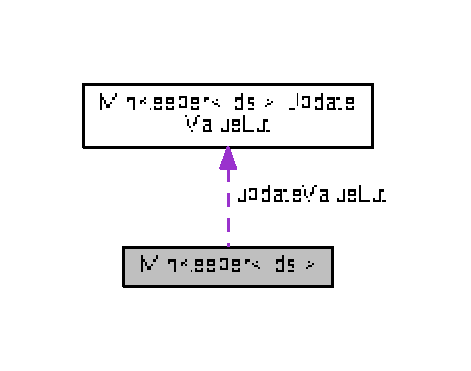
\includegraphics[width=226pt]{classMinKeeper__coll__graph}
\end{center}
\end{figure}
\subsection*{Classes}
\begin{DoxyCompactItemize}
\item 
struct \hyperlink{structMinKeeper_1_1Num}{Num}
\item 
struct \hyperlink{structMinKeeper_1_1Sum}{Sum}
\item 
struct \hyperlink{structMinKeeper_1_1UpdateValue}{Update\+Value}
\item 
struct \hyperlink{structMinKeeper_1_1UpdateValue_3_01id_00_010_01_4}{Update\+Value$<$ id, 0 $>$}
\item 
class \hyperlink{classMinKeeper_1_1UpdateValueLut}{Update\+Value\+Lut}
\end{DoxyCompactItemize}
\subsection*{Public Member Functions}
\begin{DoxyCompactItemize}
\item 
\hyperlink{classMinKeeper_a131eb12143092dbce960174124d60663}{Min\+Keeper} (unsigned init\+Value=0x\+F\+F\+F\+F\+F\+F\+F\+F)
\item 
\hyperlink{ioapi_8h_a787fa3cf048117ba7123753c1e74fcd6}{int} \hyperlink{classMinKeeper_a27b4f4cc206c7e587231929994d26705}{min} () const
\item 
unsigned \hyperlink{classMinKeeper_a92eb88a85193e36452c4b321ed7db903}{min\+Value} () const
\item 
{\footnotesize template$<$int id$>$ }\\void \hyperlink{classMinKeeper_ab74f92c2bfad235b0663a3765a716dab}{set\+Value} (unsigned cnt)
\item 
void \hyperlink{classMinKeeper_a6d2d7fa6634c14d56b1caba0efaec47c}{set\+Value} (\hyperlink{ioapi_8h_a787fa3cf048117ba7123753c1e74fcd6}{int} id, unsigned cnt)
\item 
unsigned \hyperlink{classMinKeeper_a87ea0acfa0a9bdccfacac89794bc30ce}{value} (\hyperlink{ioapi_8h_a787fa3cf048117ba7123753c1e74fcd6}{int} id) const
\item 
void \hyperlink{classMinKeeper_a00b6df8254b050b77b9c1350a0b7d386}{load\+Or\+Save} (\hyperlink{classgambatte_1_1loadsave}{gambatte\+::loadsave} \&\hyperlink{ppu_8cpp_a2f2eca6997ee7baf8901725ae074d45b}{state})
\end{DoxyCompactItemize}
\subsection*{Private Types}
\begin{DoxyCompactItemize}
\item 
enum \{ \hyperlink{classMinKeeper_a745fcad4766af72248c4f26e8fb5b754aea945fa5cad053f00154ef3bf621ea51}{levels} = Min\+Keeper\+Util\+:\+:Ceiled\+Log2$<$ids$>$\+:\+:r
 \}
\end{DoxyCompactItemize}
\subsection*{Static Private Member Functions}
\begin{DoxyCompactItemize}
\item 
{\footnotesize template$<$int id$>$ }\\static void \hyperlink{classMinKeeper_abbe4083eb661d964a091c5e5d6f0a9cf}{update\+Value} (\hyperlink{classMinKeeper}{Min\+Keeper}$<$ ids $>$ \&m)
\end{DoxyCompactItemize}
\subsection*{Private Attributes}
\begin{DoxyCompactItemize}
\item 
unsigned \hyperlink{classMinKeeper_a7096c3993486cb56ee56b7434282a5cc}{values\+\_\+} \mbox{[}ids\mbox{]}
\item 
unsigned \hyperlink{classMinKeeper_a5701ef91dc989316dfa7992c19b03ca9}{min\+Value\+\_\+}
\item 
\hyperlink{ioapi_8h_a787fa3cf048117ba7123753c1e74fcd6}{int} \hyperlink{classMinKeeper_ac5ddfd149ad4ff5b944a98ccf4b1e6cd}{a\+\_\+} \mbox{[}\hyperlink{structMinKeeper_1_1Sum}{Sum}$<$ \hyperlink{classMinKeeper_a745fcad4766af72248c4f26e8fb5b754aea945fa5cad053f00154ef3bf621ea51}{levels} $>$\+::r\mbox{]}
\end{DoxyCompactItemize}
\subsection*{Static Private Attributes}
\begin{DoxyCompactItemize}
\item 
static \hyperlink{classMinKeeper_1_1UpdateValueLut}{Update\+Value\+Lut} \hyperlink{classMinKeeper_a63181263fc50994bef542275e0962ff0}{update\+Value\+Lut}
\end{DoxyCompactItemize}


\subsection{Member Enumeration Documentation}
\mbox{\Hypertarget{classMinKeeper_a745fcad4766af72248c4f26e8fb5b754}\label{classMinKeeper_a745fcad4766af72248c4f26e8fb5b754}} 
\subsubsection{\texorpdfstring{anonymous enum}{anonymous enum}}
{\footnotesize\ttfamily template$<$int ids$>$ \\
anonymous enum\hspace{0.3cm}{\ttfamily [private]}}

\begin{DoxyEnumFields}{Enumerator}
\raisebox{\heightof{T}}[0pt][0pt]{\index{levels@{levels}!Min\+Keeper@{Min\+Keeper}}\index{Min\+Keeper@{Min\+Keeper}!levels@{levels}}}\mbox{\Hypertarget{classMinKeeper_a745fcad4766af72248c4f26e8fb5b754aea945fa5cad053f00154ef3bf621ea51}\label{classMinKeeper_a745fcad4766af72248c4f26e8fb5b754aea945fa5cad053f00154ef3bf621ea51}} 
levels&\\
\hline

\end{DoxyEnumFields}


\subsection{Constructor \& Destructor Documentation}
\mbox{\Hypertarget{classMinKeeper_a131eb12143092dbce960174124d60663}\label{classMinKeeper_a131eb12143092dbce960174124d60663}} 
\index{Min\+Keeper@{Min\+Keeper}!Min\+Keeper@{Min\+Keeper}}
\index{Min\+Keeper@{Min\+Keeper}!Min\+Keeper@{Min\+Keeper}}
\subsubsection{\texorpdfstring{Min\+Keeper()}{MinKeeper()}}
{\footnotesize\ttfamily template$<$int ids$>$ \\
\hyperlink{classMinKeeper}{Min\+Keeper}$<$ ids $>$\+::\hyperlink{classMinKeeper}{Min\+Keeper} (\begin{DoxyParamCaption}\item[{unsigned}]{init\+Value = {\ttfamily 0xFFFFFFFF} }\end{DoxyParamCaption})\hspace{0.3cm}{\ttfamily [explicit]}}



\subsection{Member Function Documentation}
\mbox{\Hypertarget{classMinKeeper_a00b6df8254b050b77b9c1350a0b7d386}\label{classMinKeeper_a00b6df8254b050b77b9c1350a0b7d386}} 
\index{Min\+Keeper@{Min\+Keeper}!load\+Or\+Save@{load\+Or\+Save}}
\index{load\+Or\+Save@{load\+Or\+Save}!Min\+Keeper@{Min\+Keeper}}
\subsubsection{\texorpdfstring{load\+Or\+Save()}{loadOrSave()}}
{\footnotesize\ttfamily template$<$int ids$>$ \\
void \hyperlink{classMinKeeper}{Min\+Keeper}$<$ ids $>$\+::load\+Or\+Save (\begin{DoxyParamCaption}\item[{\hyperlink{classgambatte_1_1loadsave}{gambatte\+::loadsave} \&}]{state }\end{DoxyParamCaption})\hspace{0.3cm}{\ttfamily [inline]}}

\mbox{\Hypertarget{classMinKeeper_a27b4f4cc206c7e587231929994d26705}\label{classMinKeeper_a27b4f4cc206c7e587231929994d26705}} 
\index{Min\+Keeper@{Min\+Keeper}!min@{min}}
\index{min@{min}!Min\+Keeper@{Min\+Keeper}}
\subsubsection{\texorpdfstring{min()}{min()}}
{\footnotesize\ttfamily template$<$int ids$>$ \\
\hyperlink{ioapi_8h_a787fa3cf048117ba7123753c1e74fcd6}{int} \hyperlink{classMinKeeper}{Min\+Keeper}$<$ ids $>$\+::min (\begin{DoxyParamCaption}{ }\end{DoxyParamCaption}) const\hspace{0.3cm}{\ttfamily [inline]}}

\mbox{\Hypertarget{classMinKeeper_a92eb88a85193e36452c4b321ed7db903}\label{classMinKeeper_a92eb88a85193e36452c4b321ed7db903}} 
\index{Min\+Keeper@{Min\+Keeper}!min\+Value@{min\+Value}}
\index{min\+Value@{min\+Value}!Min\+Keeper@{Min\+Keeper}}
\subsubsection{\texorpdfstring{min\+Value()}{minValue()}}
{\footnotesize\ttfamily template$<$int ids$>$ \\
unsigned \hyperlink{classMinKeeper}{Min\+Keeper}$<$ ids $>$\+::min\+Value (\begin{DoxyParamCaption}{ }\end{DoxyParamCaption}) const\hspace{0.3cm}{\ttfamily [inline]}}

\mbox{\Hypertarget{classMinKeeper_ab74f92c2bfad235b0663a3765a716dab}\label{classMinKeeper_ab74f92c2bfad235b0663a3765a716dab}} 
\index{Min\+Keeper@{Min\+Keeper}!set\+Value@{set\+Value}}
\index{set\+Value@{set\+Value}!Min\+Keeper@{Min\+Keeper}}
\subsubsection{\texorpdfstring{set\+Value()}{setValue()}\hspace{0.1cm}{\footnotesize\ttfamily [1/2]}}
{\footnotesize\ttfamily template$<$int ids$>$ \\
template$<$int id$>$ \\
void \hyperlink{classMinKeeper}{Min\+Keeper}$<$ ids $>$\+::set\+Value (\begin{DoxyParamCaption}\item[{unsigned}]{cnt }\end{DoxyParamCaption})\hspace{0.3cm}{\ttfamily [inline]}}

\mbox{\Hypertarget{classMinKeeper_a6d2d7fa6634c14d56b1caba0efaec47c}\label{classMinKeeper_a6d2d7fa6634c14d56b1caba0efaec47c}} 
\index{Min\+Keeper@{Min\+Keeper}!set\+Value@{set\+Value}}
\index{set\+Value@{set\+Value}!Min\+Keeper@{Min\+Keeper}}
\subsubsection{\texorpdfstring{set\+Value()}{setValue()}\hspace{0.1cm}{\footnotesize\ttfamily [2/2]}}
{\footnotesize\ttfamily template$<$int ids$>$ \\
void \hyperlink{classMinKeeper}{Min\+Keeper}$<$ ids $>$\+::set\+Value (\begin{DoxyParamCaption}\item[{\hyperlink{ioapi_8h_a787fa3cf048117ba7123753c1e74fcd6}{int}}]{id,  }\item[{unsigned}]{cnt }\end{DoxyParamCaption})\hspace{0.3cm}{\ttfamily [inline]}}

\mbox{\Hypertarget{classMinKeeper_abbe4083eb661d964a091c5e5d6f0a9cf}\label{classMinKeeper_abbe4083eb661d964a091c5e5d6f0a9cf}} 
\index{Min\+Keeper@{Min\+Keeper}!update\+Value@{update\+Value}}
\index{update\+Value@{update\+Value}!Min\+Keeper@{Min\+Keeper}}
\subsubsection{\texorpdfstring{update\+Value()}{updateValue()}}
{\footnotesize\ttfamily template$<$int ids$>$ \\
template$<$int id$>$ \\
void \hyperlink{classMinKeeper}{Min\+Keeper}$<$ ids $>$\+::update\+Value (\begin{DoxyParamCaption}\item[{\hyperlink{classMinKeeper}{Min\+Keeper}$<$ ids $>$ \&}]{m }\end{DoxyParamCaption})\hspace{0.3cm}{\ttfamily [static]}, {\ttfamily [private]}}

\mbox{\Hypertarget{classMinKeeper_a87ea0acfa0a9bdccfacac89794bc30ce}\label{classMinKeeper_a87ea0acfa0a9bdccfacac89794bc30ce}} 
\index{Min\+Keeper@{Min\+Keeper}!value@{value}}
\index{value@{value}!Min\+Keeper@{Min\+Keeper}}
\subsubsection{\texorpdfstring{value()}{value()}}
{\footnotesize\ttfamily template$<$int ids$>$ \\
unsigned \hyperlink{classMinKeeper}{Min\+Keeper}$<$ ids $>$\+::value (\begin{DoxyParamCaption}\item[{\hyperlink{ioapi_8h_a787fa3cf048117ba7123753c1e74fcd6}{int}}]{id }\end{DoxyParamCaption}) const\hspace{0.3cm}{\ttfamily [inline]}}



\subsection{Member Data Documentation}
\mbox{\Hypertarget{classMinKeeper_ac5ddfd149ad4ff5b944a98ccf4b1e6cd}\label{classMinKeeper_ac5ddfd149ad4ff5b944a98ccf4b1e6cd}} 
\index{Min\+Keeper@{Min\+Keeper}!a\+\_\+@{a\+\_\+}}
\index{a\+\_\+@{a\+\_\+}!Min\+Keeper@{Min\+Keeper}}
\subsubsection{\texorpdfstring{a\+\_\+}{a\_}}
{\footnotesize\ttfamily template$<$int ids$>$ \\
\hyperlink{ioapi_8h_a787fa3cf048117ba7123753c1e74fcd6}{int} \hyperlink{classMinKeeper}{Min\+Keeper}$<$ ids $>$\+::a\+\_\+\mbox{[}\hyperlink{structMinKeeper_1_1Sum}{Sum}$<$ \hyperlink{classMinKeeper_a745fcad4766af72248c4f26e8fb5b754aea945fa5cad053f00154ef3bf621ea51}{levels} $>$\+::r\mbox{]}\hspace{0.3cm}{\ttfamily [private]}}

\mbox{\Hypertarget{classMinKeeper_a5701ef91dc989316dfa7992c19b03ca9}\label{classMinKeeper_a5701ef91dc989316dfa7992c19b03ca9}} 
\index{Min\+Keeper@{Min\+Keeper}!min\+Value\+\_\+@{min\+Value\+\_\+}}
\index{min\+Value\+\_\+@{min\+Value\+\_\+}!Min\+Keeper@{Min\+Keeper}}
\subsubsection{\texorpdfstring{min\+Value\+\_\+}{minValue\_}}
{\footnotesize\ttfamily template$<$int ids$>$ \\
unsigned \hyperlink{classMinKeeper}{Min\+Keeper}$<$ ids $>$\+::min\+Value\+\_\+\hspace{0.3cm}{\ttfamily [private]}}

\mbox{\Hypertarget{classMinKeeper_a63181263fc50994bef542275e0962ff0}\label{classMinKeeper_a63181263fc50994bef542275e0962ff0}} 
\index{Min\+Keeper@{Min\+Keeper}!update\+Value\+Lut@{update\+Value\+Lut}}
\index{update\+Value\+Lut@{update\+Value\+Lut}!Min\+Keeper@{Min\+Keeper}}
\subsubsection{\texorpdfstring{update\+Value\+Lut}{updateValueLut}}
{\footnotesize\ttfamily template$<$int ids$>$ \\
\hyperlink{classMinKeeper}{Min\+Keeper}$<$ ids $>$\+::\hyperlink{classMinKeeper_1_1UpdateValueLut}{Update\+Value\+Lut} \hyperlink{classMinKeeper}{Min\+Keeper}$<$ ids $>$\+::update\+Value\+Lut\hspace{0.3cm}{\ttfamily [static]}, {\ttfamily [private]}}

\mbox{\Hypertarget{classMinKeeper_a7096c3993486cb56ee56b7434282a5cc}\label{classMinKeeper_a7096c3993486cb56ee56b7434282a5cc}} 
\index{Min\+Keeper@{Min\+Keeper}!values\+\_\+@{values\+\_\+}}
\index{values\+\_\+@{values\+\_\+}!Min\+Keeper@{Min\+Keeper}}
\subsubsection{\texorpdfstring{values\+\_\+}{values\_}}
{\footnotesize\ttfamily template$<$int ids$>$ \\
unsigned \hyperlink{classMinKeeper}{Min\+Keeper}$<$ ids $>$\+::values\+\_\+\mbox{[}ids\mbox{]}\hspace{0.3cm}{\ttfamily [private]}}



The documentation for this class was generated from the following file\+:\begin{DoxyCompactItemize}
\item 
src/\hyperlink{minkeeper_8h}{minkeeper.\+h}\end{DoxyCompactItemize}

\hypertarget{classgambatte_1_1NextM0Time}{}\section{gambatte\+:\+:Next\+M0\+Time Class Reference}
\label{classgambatte_1_1NextM0Time}\index{gambatte\+::\+Next\+M0\+Time@{gambatte\+::\+Next\+M0\+Time}}


{\ttfamily \#include $<$next\+\_\+m0\+\_\+time.\+h$>$}

\subsection*{Public Member Functions}
\begin{DoxyCompactItemize}
\item 
\hyperlink{classgambatte_1_1NextM0Time_a0b0c1ec8902b1a108f70ddef805e6b3d}{Next\+M0\+Time} ()
\item 
void \hyperlink{classgambatte_1_1NextM0Time_afcfab2f5281e94db443bd07981720092}{predict\+Next\+M0\+Time} (class \hyperlink{classgambatte_1_1PPU}{P\+PU} const \&v)
\item 
void \hyperlink{classgambatte_1_1NextM0Time_ac43a95dccad6a368419308a78e9f61a5}{invalidate\+Predicted\+Next\+M0\+Time} ()
\item 
unsigned \hyperlink{classgambatte_1_1NextM0Time_a6eab539b211eeb7c88fb0b72ca10e079}{predicted\+Next\+M0\+Time} () const
\item 
void \hyperlink{classgambatte_1_1NextM0Time_a6f94512bb082af935c4b381fc6d16c93}{load\+Or\+Save} (\hyperlink{classgambatte_1_1loadsave}{loadsave} \&\hyperlink{ppu_8cpp_a2f2eca6997ee7baf8901725ae074d45b}{state})
\end{DoxyCompactItemize}
\subsection*{Private Attributes}
\begin{DoxyCompactItemize}
\item 
unsigned \hyperlink{classgambatte_1_1NextM0Time_ac193efbcd78f7c6c44eba906eecc3abe}{predicted\+Next\+M0\+Time\+\_\+}
\end{DoxyCompactItemize}


\subsection{Constructor \& Destructor Documentation}
\mbox{\Hypertarget{classgambatte_1_1NextM0Time_a0b0c1ec8902b1a108f70ddef805e6b3d}\label{classgambatte_1_1NextM0Time_a0b0c1ec8902b1a108f70ddef805e6b3d}} 
\index{gambatte\+::\+Next\+M0\+Time@{gambatte\+::\+Next\+M0\+Time}!Next\+M0\+Time@{Next\+M0\+Time}}
\index{Next\+M0\+Time@{Next\+M0\+Time}!gambatte\+::\+Next\+M0\+Time@{gambatte\+::\+Next\+M0\+Time}}
\subsubsection{\texorpdfstring{Next\+M0\+Time()}{NextM0Time()}}
{\footnotesize\ttfamily gambatte\+::\+Next\+M0\+Time\+::\+Next\+M0\+Time (\begin{DoxyParamCaption}{ }\end{DoxyParamCaption})\hspace{0.3cm}{\ttfamily [inline]}}



\subsection{Member Function Documentation}
\mbox{\Hypertarget{classgambatte_1_1NextM0Time_ac43a95dccad6a368419308a78e9f61a5}\label{classgambatte_1_1NextM0Time_ac43a95dccad6a368419308a78e9f61a5}} 
\index{gambatte\+::\+Next\+M0\+Time@{gambatte\+::\+Next\+M0\+Time}!invalidate\+Predicted\+Next\+M0\+Time@{invalidate\+Predicted\+Next\+M0\+Time}}
\index{invalidate\+Predicted\+Next\+M0\+Time@{invalidate\+Predicted\+Next\+M0\+Time}!gambatte\+::\+Next\+M0\+Time@{gambatte\+::\+Next\+M0\+Time}}
\subsubsection{\texorpdfstring{invalidate\+Predicted\+Next\+M0\+Time()}{invalidatePredictedNextM0Time()}}
{\footnotesize\ttfamily void gambatte\+::\+Next\+M0\+Time\+::invalidate\+Predicted\+Next\+M0\+Time (\begin{DoxyParamCaption}{ }\end{DoxyParamCaption})\hspace{0.3cm}{\ttfamily [inline]}}

\mbox{\Hypertarget{classgambatte_1_1NextM0Time_a6f94512bb082af935c4b381fc6d16c93}\label{classgambatte_1_1NextM0Time_a6f94512bb082af935c4b381fc6d16c93}} 
\index{gambatte\+::\+Next\+M0\+Time@{gambatte\+::\+Next\+M0\+Time}!load\+Or\+Save@{load\+Or\+Save}}
\index{load\+Or\+Save@{load\+Or\+Save}!gambatte\+::\+Next\+M0\+Time@{gambatte\+::\+Next\+M0\+Time}}
\subsubsection{\texorpdfstring{load\+Or\+Save()}{loadOrSave()}}
{\footnotesize\ttfamily void gambatte\+::\+Next\+M0\+Time\+::load\+Or\+Save (\begin{DoxyParamCaption}\item[{\hyperlink{classgambatte_1_1loadsave}{loadsave} \&}]{state }\end{DoxyParamCaption})\hspace{0.3cm}{\ttfamily [inline]}}

\mbox{\Hypertarget{classgambatte_1_1NextM0Time_a6eab539b211eeb7c88fb0b72ca10e079}\label{classgambatte_1_1NextM0Time_a6eab539b211eeb7c88fb0b72ca10e079}} 
\index{gambatte\+::\+Next\+M0\+Time@{gambatte\+::\+Next\+M0\+Time}!predicted\+Next\+M0\+Time@{predicted\+Next\+M0\+Time}}
\index{predicted\+Next\+M0\+Time@{predicted\+Next\+M0\+Time}!gambatte\+::\+Next\+M0\+Time@{gambatte\+::\+Next\+M0\+Time}}
\subsubsection{\texorpdfstring{predicted\+Next\+M0\+Time()}{predictedNextM0Time()}}
{\footnotesize\ttfamily unsigned gambatte\+::\+Next\+M0\+Time\+::predicted\+Next\+M0\+Time (\begin{DoxyParamCaption}{ }\end{DoxyParamCaption}) const\hspace{0.3cm}{\ttfamily [inline]}}

\mbox{\Hypertarget{classgambatte_1_1NextM0Time_afcfab2f5281e94db443bd07981720092}\label{classgambatte_1_1NextM0Time_afcfab2f5281e94db443bd07981720092}} 
\index{gambatte\+::\+Next\+M0\+Time@{gambatte\+::\+Next\+M0\+Time}!predict\+Next\+M0\+Time@{predict\+Next\+M0\+Time}}
\index{predict\+Next\+M0\+Time@{predict\+Next\+M0\+Time}!gambatte\+::\+Next\+M0\+Time@{gambatte\+::\+Next\+M0\+Time}}
\subsubsection{\texorpdfstring{predict\+Next\+M0\+Time()}{predictNextM0Time()}}
{\footnotesize\ttfamily void gambatte\+::\+Next\+M0\+Time\+::predict\+Next\+M0\+Time (\begin{DoxyParamCaption}\item[{class \hyperlink{classgambatte_1_1PPU}{P\+PU} const \&}]{v }\end{DoxyParamCaption})}



\subsection{Member Data Documentation}
\mbox{\Hypertarget{classgambatte_1_1NextM0Time_ac193efbcd78f7c6c44eba906eecc3abe}\label{classgambatte_1_1NextM0Time_ac193efbcd78f7c6c44eba906eecc3abe}} 
\index{gambatte\+::\+Next\+M0\+Time@{gambatte\+::\+Next\+M0\+Time}!predicted\+Next\+M0\+Time\+\_\+@{predicted\+Next\+M0\+Time\+\_\+}}
\index{predicted\+Next\+M0\+Time\+\_\+@{predicted\+Next\+M0\+Time\+\_\+}!gambatte\+::\+Next\+M0\+Time@{gambatte\+::\+Next\+M0\+Time}}
\subsubsection{\texorpdfstring{predicted\+Next\+M0\+Time\+\_\+}{predictedNextM0Time\_}}
{\footnotesize\ttfamily unsigned gambatte\+::\+Next\+M0\+Time\+::predicted\+Next\+M0\+Time\+\_\+\hspace{0.3cm}{\ttfamily [private]}}



The documentation for this class was generated from the following files\+:\begin{DoxyCompactItemize}
\item 
src/video/\hyperlink{next__m0__time_8h}{next\+\_\+m0\+\_\+time.\+h}\item 
src/video/\hyperlink{next__m0__time_8cpp}{next\+\_\+m0\+\_\+time.\+cpp}\end{DoxyCompactItemize}

\hypertarget{structMinKeeper_1_1Num}{}\section{Min\+Keeper$<$ ids $>$\+:\+:Num$<$ l $>$ Struct Template Reference}
\label{structMinKeeper_1_1Num}\index{Min\+Keeper$<$ ids $>$\+::\+Num$<$ l $>$@{Min\+Keeper$<$ ids $>$\+::\+Num$<$ l $>$}}
\subsection*{Public Types}
\begin{DoxyCompactItemize}
\item 
enum \{ \hyperlink{structMinKeeper_1_1Num_aa17330c307108c34ace840974c85e724aee045d9ab47b61ac5537035973fe9cea}{r} = Min\+Keeper\+Util\+:\+:Rounded\+Div2n$<$ids, levels + 1 -\/ l$>$\+:\+:r
 \}
\end{DoxyCompactItemize}


\subsection{Member Enumeration Documentation}
\mbox{\Hypertarget{structMinKeeper_1_1Num_aa17330c307108c34ace840974c85e724}\label{structMinKeeper_1_1Num_aa17330c307108c34ace840974c85e724}} 
\subsubsection{\texorpdfstring{anonymous enum}{anonymous enum}}
{\footnotesize\ttfamily template$<$int ids$>$ \\
template$<$int l$>$ \\
anonymous enum}

\begin{DoxyEnumFields}{Enumerator}
\raisebox{\heightof{T}}[0pt][0pt]{\index{r@{r}!Min\+Keeper\+::\+Num@{Min\+Keeper\+::\+Num}}\index{Min\+Keeper\+::\+Num@{Min\+Keeper\+::\+Num}!r@{r}}}\mbox{\Hypertarget{structMinKeeper_1_1Num_aa17330c307108c34ace840974c85e724aee045d9ab47b61ac5537035973fe9cea}\label{structMinKeeper_1_1Num_aa17330c307108c34ace840974c85e724aee045d9ab47b61ac5537035973fe9cea}} 
r&\\
\hline

\end{DoxyEnumFields}


The documentation for this struct was generated from the following file\+:\begin{DoxyCompactItemize}
\item 
src/\hyperlink{minkeeper_8h}{minkeeper.\+h}\end{DoxyCompactItemize}

\hypertarget{classgambatte_1_1SpriteMapper_1_1OamReader}{}\section{gambatte\+:\+:Sprite\+Mapper\+:\+:Oam\+Reader Class Reference}
\label{classgambatte_1_1SpriteMapper_1_1OamReader}\index{gambatte\+::\+Sprite\+Mapper\+::\+Oam\+Reader@{gambatte\+::\+Sprite\+Mapper\+::\+Oam\+Reader}}


Collaboration diagram for gambatte\+:\+:Sprite\+Mapper\+:\+:Oam\+Reader\+:
\nopagebreak
\begin{figure}[H]
\begin{center}
\leavevmode
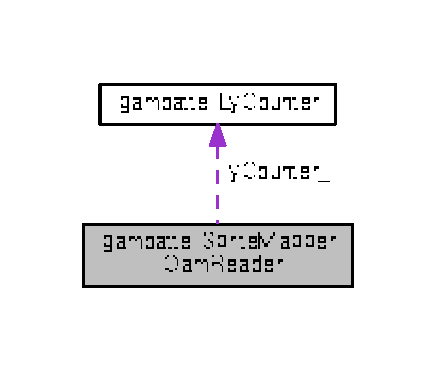
\includegraphics[width=209pt]{classgambatte_1_1SpriteMapper_1_1OamReader__coll__graph}
\end{center}
\end{figure}
\subsection*{Public Member Functions}
\begin{DoxyCompactItemize}
\item 
void \hyperlink{classgambatte_1_1SpriteMapper_1_1OamReader_a4c2aae2820fbaa3fb2d14c85f7ceb8de}{load\+Or\+Save} (\hyperlink{classgambatte_1_1loadsave}{loadsave} \&\hyperlink{ppu_8cpp_a2f2eca6997ee7baf8901725ae074d45b}{state})
\item 
\hyperlink{classgambatte_1_1SpriteMapper_1_1OamReader_ab65ab121f0685f5ef664a01bef316dbe}{Oam\+Reader} (\hyperlink{classgambatte_1_1LyCounter}{Ly\+Counter} const \&ly\+Counter, unsigned char const $\ast$\hyperlink{classgambatte_1_1SpriteMapper_a558ee1ff5817b79285f7cc91d627535b}{oamram})
\item 
void \hyperlink{classgambatte_1_1SpriteMapper_1_1OamReader_a2a361f2224f240eef6db7147fffbdcad}{reset} (unsigned char const $\ast$\hyperlink{classgambatte_1_1SpriteMapper_a558ee1ff5817b79285f7cc91d627535b}{oamram}, bool cgb)
\item 
void \hyperlink{classgambatte_1_1SpriteMapper_1_1OamReader_a94194013dbb68d7b9fee10f999f80bfe}{change} (unsigned cc)
\item 
void \hyperlink{classgambatte_1_1SpriteMapper_1_1OamReader_a47d768d577cc3f3a0c4c28224242f487}{change} (unsigned char const $\ast$\hyperlink{classgambatte_1_1SpriteMapper_a558ee1ff5817b79285f7cc91d627535b}{oamram}, unsigned cc)
\item 
bool \hyperlink{classgambatte_1_1SpriteMapper_1_1OamReader_a5b23ae57f747ce78786621a118695359}{changed} () const
\item 
bool \hyperlink{classgambatte_1_1SpriteMapper_1_1OamReader_aa00071e80166eda7afe79d9215f1085f}{large\+Sprites} (unsigned sp\+No) const
\item 
unsigned char const  $\ast$ \hyperlink{classgambatte_1_1SpriteMapper_1_1OamReader_a9b665fd4fef3a720ea2c859b1ebe0c63}{oam} () const
\item 
void \hyperlink{classgambatte_1_1SpriteMapper_1_1OamReader_a7b4142f1bec0aa8f2e30198724628d62}{reset\+Cycle\+Counter} (unsigned old\+Cc, unsigned new\+Cc)
\item 
void \hyperlink{classgambatte_1_1SpriteMapper_1_1OamReader_aca75b2d751e52e1f234da3d97cb17f8f}{set\+Large\+Sprites\+Src} (bool src)
\item 
void \hyperlink{classgambatte_1_1SpriteMapper_1_1OamReader_aed95204d144dd7d7f2cc885bf439991d}{update} (unsigned cc)
\item 
unsigned char const  $\ast$ \hyperlink{classgambatte_1_1SpriteMapper_1_1OamReader_a3080a3d42e877551ec8dde8724223053}{sprite\+Pos\+Buf} () const
\item 
void \hyperlink{classgambatte_1_1SpriteMapper_1_1OamReader_a8d8e0989e0c2ae58034ed6c08be33bc9}{set\+State\+Ptrs} (\hyperlink{structgambatte_1_1SaveState}{Save\+State} \&\hyperlink{ppu_8cpp_a2f2eca6997ee7baf8901725ae074d45b}{state})
\item 
void \hyperlink{classgambatte_1_1SpriteMapper_1_1OamReader_ac59cd90aa85b5155eb6ab14dc6f01115}{enable\+Display} (unsigned cc)
\item 
void \hyperlink{classgambatte_1_1SpriteMapper_1_1OamReader_a937011ba446debb723dbb3ae98007936}{save\+State} (\hyperlink{structgambatte_1_1SaveState}{Save\+State} \&\hyperlink{ppu_8cpp_a2f2eca6997ee7baf8901725ae074d45b}{state}) const
\item 
void \hyperlink{classgambatte_1_1SpriteMapper_1_1OamReader_a58347ffdbab3873820b3570cbca370b0}{load\+State} (\hyperlink{structgambatte_1_1SaveState}{Save\+State} const \&ss, unsigned char const $\ast$\hyperlink{classgambatte_1_1SpriteMapper_a558ee1ff5817b79285f7cc91d627535b}{oamram})
\item 
bool \hyperlink{classgambatte_1_1SpriteMapper_1_1OamReader_ae3864e972f2371a24a0bdbe849b4d6fa}{inactive\+Period\+After\+Display\+Enable} (unsigned cc) const
\item 
unsigned \hyperlink{classgambatte_1_1SpriteMapper_1_1OamReader_a4a3b93efd1551abe299c9274473286af}{line\+Time} () const
\end{DoxyCompactItemize}
\subsection*{Private Attributes}
\begin{DoxyCompactItemize}
\item 
unsigned char \hyperlink{classgambatte_1_1SpriteMapper_1_1OamReader_acc0df0fc3ac6e5b0ec5535a764456220}{buf\+\_\+} \mbox{[}80\mbox{]}
\item 
bool \hyperlink{classgambatte_1_1SpriteMapper_1_1OamReader_a283726945791824e8b354e79bc8b4b2c}{szbuf\+\_\+} \mbox{[}40\mbox{]}
\item 
\hyperlink{classgambatte_1_1LyCounter}{Ly\+Counter} const  \& \hyperlink{classgambatte_1_1SpriteMapper_1_1OamReader_a907ad5bb63d28f834455285f6acd57a9}{ly\+Counter\+\_\+}
\item 
unsigned char const  $\ast$ \hyperlink{classgambatte_1_1SpriteMapper_1_1OamReader_acaae688f585201999a41b5aade0726d3}{oamram\+\_\+}
\item 
unsigned \hyperlink{classgambatte_1_1SpriteMapper_1_1OamReader_ae5502dcd770a8dd4ce083532813ea352}{lu\+\_\+}
\item 
unsigned char \hyperlink{classgambatte_1_1SpriteMapper_1_1OamReader_ae77a7aa0390ff2bd933e712802865767}{last\+Change\+\_\+}
\item 
bool \hyperlink{classgambatte_1_1SpriteMapper_1_1OamReader_a4601e1179ad370e055a57c973d999c2d}{large\+Sprites\+Src\+\_\+}
\item 
bool \hyperlink{classgambatte_1_1SpriteMapper_1_1OamReader_abd5aa0b077b867e4bdf3971c34cb6bb7}{cgb\+\_\+}
\end{DoxyCompactItemize}


\subsection{Constructor \& Destructor Documentation}
\mbox{\Hypertarget{classgambatte_1_1SpriteMapper_1_1OamReader_ab65ab121f0685f5ef664a01bef316dbe}\label{classgambatte_1_1SpriteMapper_1_1OamReader_ab65ab121f0685f5ef664a01bef316dbe}} 
\index{gambatte\+::\+Sprite\+Mapper\+::\+Oam\+Reader@{gambatte\+::\+Sprite\+Mapper\+::\+Oam\+Reader}!Oam\+Reader@{Oam\+Reader}}
\index{Oam\+Reader@{Oam\+Reader}!gambatte\+::\+Sprite\+Mapper\+::\+Oam\+Reader@{gambatte\+::\+Sprite\+Mapper\+::\+Oam\+Reader}}
\subsubsection{\texorpdfstring{Oam\+Reader()}{OamReader()}}
{\footnotesize\ttfamily gambatte\+::\+Sprite\+Mapper\+::\+Oam\+Reader\+::\+Oam\+Reader (\begin{DoxyParamCaption}\item[{\hyperlink{classgambatte_1_1LyCounter}{Ly\+Counter} const \&}]{ly\+Counter,  }\item[{unsigned char const $\ast$}]{oamram }\end{DoxyParamCaption})}



\subsection{Member Function Documentation}
\mbox{\Hypertarget{classgambatte_1_1SpriteMapper_1_1OamReader_a94194013dbb68d7b9fee10f999f80bfe}\label{classgambatte_1_1SpriteMapper_1_1OamReader_a94194013dbb68d7b9fee10f999f80bfe}} 
\index{gambatte\+::\+Sprite\+Mapper\+::\+Oam\+Reader@{gambatte\+::\+Sprite\+Mapper\+::\+Oam\+Reader}!change@{change}}
\index{change@{change}!gambatte\+::\+Sprite\+Mapper\+::\+Oam\+Reader@{gambatte\+::\+Sprite\+Mapper\+::\+Oam\+Reader}}
\subsubsection{\texorpdfstring{change()}{change()}\hspace{0.1cm}{\footnotesize\ttfamily [1/2]}}
{\footnotesize\ttfamily void gambatte\+::\+Sprite\+Mapper\+::\+Oam\+Reader\+::change (\begin{DoxyParamCaption}\item[{unsigned}]{cc }\end{DoxyParamCaption})}

\mbox{\Hypertarget{classgambatte_1_1SpriteMapper_1_1OamReader_a47d768d577cc3f3a0c4c28224242f487}\label{classgambatte_1_1SpriteMapper_1_1OamReader_a47d768d577cc3f3a0c4c28224242f487}} 
\index{gambatte\+::\+Sprite\+Mapper\+::\+Oam\+Reader@{gambatte\+::\+Sprite\+Mapper\+::\+Oam\+Reader}!change@{change}}
\index{change@{change}!gambatte\+::\+Sprite\+Mapper\+::\+Oam\+Reader@{gambatte\+::\+Sprite\+Mapper\+::\+Oam\+Reader}}
\subsubsection{\texorpdfstring{change()}{change()}\hspace{0.1cm}{\footnotesize\ttfamily [2/2]}}
{\footnotesize\ttfamily void gambatte\+::\+Sprite\+Mapper\+::\+Oam\+Reader\+::change (\begin{DoxyParamCaption}\item[{unsigned char const $\ast$}]{oamram,  }\item[{unsigned}]{cc }\end{DoxyParamCaption})\hspace{0.3cm}{\ttfamily [inline]}}

\mbox{\Hypertarget{classgambatte_1_1SpriteMapper_1_1OamReader_a5b23ae57f747ce78786621a118695359}\label{classgambatte_1_1SpriteMapper_1_1OamReader_a5b23ae57f747ce78786621a118695359}} 
\index{gambatte\+::\+Sprite\+Mapper\+::\+Oam\+Reader@{gambatte\+::\+Sprite\+Mapper\+::\+Oam\+Reader}!changed@{changed}}
\index{changed@{changed}!gambatte\+::\+Sprite\+Mapper\+::\+Oam\+Reader@{gambatte\+::\+Sprite\+Mapper\+::\+Oam\+Reader}}
\subsubsection{\texorpdfstring{changed()}{changed()}}
{\footnotesize\ttfamily bool gambatte\+::\+Sprite\+Mapper\+::\+Oam\+Reader\+::changed (\begin{DoxyParamCaption}{ }\end{DoxyParamCaption}) const\hspace{0.3cm}{\ttfamily [inline]}}

\mbox{\Hypertarget{classgambatte_1_1SpriteMapper_1_1OamReader_ac59cd90aa85b5155eb6ab14dc6f01115}\label{classgambatte_1_1SpriteMapper_1_1OamReader_ac59cd90aa85b5155eb6ab14dc6f01115}} 
\index{gambatte\+::\+Sprite\+Mapper\+::\+Oam\+Reader@{gambatte\+::\+Sprite\+Mapper\+::\+Oam\+Reader}!enable\+Display@{enable\+Display}}
\index{enable\+Display@{enable\+Display}!gambatte\+::\+Sprite\+Mapper\+::\+Oam\+Reader@{gambatte\+::\+Sprite\+Mapper\+::\+Oam\+Reader}}
\subsubsection{\texorpdfstring{enable\+Display()}{enableDisplay()}}
{\footnotesize\ttfamily void gambatte\+::\+Sprite\+Mapper\+::\+Oam\+Reader\+::enable\+Display (\begin{DoxyParamCaption}\item[{unsigned}]{cc }\end{DoxyParamCaption})}

\mbox{\Hypertarget{classgambatte_1_1SpriteMapper_1_1OamReader_ae3864e972f2371a24a0bdbe849b4d6fa}\label{classgambatte_1_1SpriteMapper_1_1OamReader_ae3864e972f2371a24a0bdbe849b4d6fa}} 
\index{gambatte\+::\+Sprite\+Mapper\+::\+Oam\+Reader@{gambatte\+::\+Sprite\+Mapper\+::\+Oam\+Reader}!inactive\+Period\+After\+Display\+Enable@{inactive\+Period\+After\+Display\+Enable}}
\index{inactive\+Period\+After\+Display\+Enable@{inactive\+Period\+After\+Display\+Enable}!gambatte\+::\+Sprite\+Mapper\+::\+Oam\+Reader@{gambatte\+::\+Sprite\+Mapper\+::\+Oam\+Reader}}
\subsubsection{\texorpdfstring{inactive\+Period\+After\+Display\+Enable()}{inactivePeriodAfterDisplayEnable()}}
{\footnotesize\ttfamily bool gambatte\+::\+Sprite\+Mapper\+::\+Oam\+Reader\+::inactive\+Period\+After\+Display\+Enable (\begin{DoxyParamCaption}\item[{unsigned}]{cc }\end{DoxyParamCaption}) const\hspace{0.3cm}{\ttfamily [inline]}}

\mbox{\Hypertarget{classgambatte_1_1SpriteMapper_1_1OamReader_aa00071e80166eda7afe79d9215f1085f}\label{classgambatte_1_1SpriteMapper_1_1OamReader_aa00071e80166eda7afe79d9215f1085f}} 
\index{gambatte\+::\+Sprite\+Mapper\+::\+Oam\+Reader@{gambatte\+::\+Sprite\+Mapper\+::\+Oam\+Reader}!large\+Sprites@{large\+Sprites}}
\index{large\+Sprites@{large\+Sprites}!gambatte\+::\+Sprite\+Mapper\+::\+Oam\+Reader@{gambatte\+::\+Sprite\+Mapper\+::\+Oam\+Reader}}
\subsubsection{\texorpdfstring{large\+Sprites()}{largeSprites()}}
{\footnotesize\ttfamily bool gambatte\+::\+Sprite\+Mapper\+::\+Oam\+Reader\+::large\+Sprites (\begin{DoxyParamCaption}\item[{unsigned}]{sp\+No }\end{DoxyParamCaption}) const\hspace{0.3cm}{\ttfamily [inline]}}

\mbox{\Hypertarget{classgambatte_1_1SpriteMapper_1_1OamReader_a4a3b93efd1551abe299c9274473286af}\label{classgambatte_1_1SpriteMapper_1_1OamReader_a4a3b93efd1551abe299c9274473286af}} 
\index{gambatte\+::\+Sprite\+Mapper\+::\+Oam\+Reader@{gambatte\+::\+Sprite\+Mapper\+::\+Oam\+Reader}!line\+Time@{line\+Time}}
\index{line\+Time@{line\+Time}!gambatte\+::\+Sprite\+Mapper\+::\+Oam\+Reader@{gambatte\+::\+Sprite\+Mapper\+::\+Oam\+Reader}}
\subsubsection{\texorpdfstring{line\+Time()}{lineTime()}}
{\footnotesize\ttfamily unsigned gambatte\+::\+Sprite\+Mapper\+::\+Oam\+Reader\+::line\+Time (\begin{DoxyParamCaption}{ }\end{DoxyParamCaption}) const\hspace{0.3cm}{\ttfamily [inline]}}

\mbox{\Hypertarget{classgambatte_1_1SpriteMapper_1_1OamReader_a4c2aae2820fbaa3fb2d14c85f7ceb8de}\label{classgambatte_1_1SpriteMapper_1_1OamReader_a4c2aae2820fbaa3fb2d14c85f7ceb8de}} 
\index{gambatte\+::\+Sprite\+Mapper\+::\+Oam\+Reader@{gambatte\+::\+Sprite\+Mapper\+::\+Oam\+Reader}!load\+Or\+Save@{load\+Or\+Save}}
\index{load\+Or\+Save@{load\+Or\+Save}!gambatte\+::\+Sprite\+Mapper\+::\+Oam\+Reader@{gambatte\+::\+Sprite\+Mapper\+::\+Oam\+Reader}}
\subsubsection{\texorpdfstring{load\+Or\+Save()}{loadOrSave()}}
{\footnotesize\ttfamily void gambatte\+::\+Sprite\+Mapper\+::\+Oam\+Reader\+::load\+Or\+Save (\begin{DoxyParamCaption}\item[{\hyperlink{classgambatte_1_1loadsave}{loadsave} \&}]{state }\end{DoxyParamCaption})\hspace{0.3cm}{\ttfamily [inline]}}

\mbox{\Hypertarget{classgambatte_1_1SpriteMapper_1_1OamReader_a58347ffdbab3873820b3570cbca370b0}\label{classgambatte_1_1SpriteMapper_1_1OamReader_a58347ffdbab3873820b3570cbca370b0}} 
\index{gambatte\+::\+Sprite\+Mapper\+::\+Oam\+Reader@{gambatte\+::\+Sprite\+Mapper\+::\+Oam\+Reader}!load\+State@{load\+State}}
\index{load\+State@{load\+State}!gambatte\+::\+Sprite\+Mapper\+::\+Oam\+Reader@{gambatte\+::\+Sprite\+Mapper\+::\+Oam\+Reader}}
\subsubsection{\texorpdfstring{load\+State()}{loadState()}}
{\footnotesize\ttfamily void gambatte\+::\+Sprite\+Mapper\+::\+Oam\+Reader\+::load\+State (\begin{DoxyParamCaption}\item[{\hyperlink{structgambatte_1_1SaveState}{Save\+State} const \&}]{ss,  }\item[{unsigned char const $\ast$}]{oamram }\end{DoxyParamCaption})}

\mbox{\Hypertarget{classgambatte_1_1SpriteMapper_1_1OamReader_a9b665fd4fef3a720ea2c859b1ebe0c63}\label{classgambatte_1_1SpriteMapper_1_1OamReader_a9b665fd4fef3a720ea2c859b1ebe0c63}} 
\index{gambatte\+::\+Sprite\+Mapper\+::\+Oam\+Reader@{gambatte\+::\+Sprite\+Mapper\+::\+Oam\+Reader}!oam@{oam}}
\index{oam@{oam}!gambatte\+::\+Sprite\+Mapper\+::\+Oam\+Reader@{gambatte\+::\+Sprite\+Mapper\+::\+Oam\+Reader}}
\subsubsection{\texorpdfstring{oam()}{oam()}}
{\footnotesize\ttfamily unsigned char const$\ast$ gambatte\+::\+Sprite\+Mapper\+::\+Oam\+Reader\+::oam (\begin{DoxyParamCaption}{ }\end{DoxyParamCaption}) const\hspace{0.3cm}{\ttfamily [inline]}}

\mbox{\Hypertarget{classgambatte_1_1SpriteMapper_1_1OamReader_a2a361f2224f240eef6db7147fffbdcad}\label{classgambatte_1_1SpriteMapper_1_1OamReader_a2a361f2224f240eef6db7147fffbdcad}} 
\index{gambatte\+::\+Sprite\+Mapper\+::\+Oam\+Reader@{gambatte\+::\+Sprite\+Mapper\+::\+Oam\+Reader}!reset@{reset}}
\index{reset@{reset}!gambatte\+::\+Sprite\+Mapper\+::\+Oam\+Reader@{gambatte\+::\+Sprite\+Mapper\+::\+Oam\+Reader}}
\subsubsection{\texorpdfstring{reset()}{reset()}}
{\footnotesize\ttfamily void gambatte\+::\+Sprite\+Mapper\+::\+Oam\+Reader\+::reset (\begin{DoxyParamCaption}\item[{unsigned char const $\ast$}]{oamram,  }\item[{bool}]{cgb }\end{DoxyParamCaption})}

\mbox{\Hypertarget{classgambatte_1_1SpriteMapper_1_1OamReader_a7b4142f1bec0aa8f2e30198724628d62}\label{classgambatte_1_1SpriteMapper_1_1OamReader_a7b4142f1bec0aa8f2e30198724628d62}} 
\index{gambatte\+::\+Sprite\+Mapper\+::\+Oam\+Reader@{gambatte\+::\+Sprite\+Mapper\+::\+Oam\+Reader}!reset\+Cycle\+Counter@{reset\+Cycle\+Counter}}
\index{reset\+Cycle\+Counter@{reset\+Cycle\+Counter}!gambatte\+::\+Sprite\+Mapper\+::\+Oam\+Reader@{gambatte\+::\+Sprite\+Mapper\+::\+Oam\+Reader}}
\subsubsection{\texorpdfstring{reset\+Cycle\+Counter()}{resetCycleCounter()}}
{\footnotesize\ttfamily void gambatte\+::\+Sprite\+Mapper\+::\+Oam\+Reader\+::reset\+Cycle\+Counter (\begin{DoxyParamCaption}\item[{unsigned}]{old\+Cc,  }\item[{unsigned}]{new\+Cc }\end{DoxyParamCaption})\hspace{0.3cm}{\ttfamily [inline]}}

\mbox{\Hypertarget{classgambatte_1_1SpriteMapper_1_1OamReader_a937011ba446debb723dbb3ae98007936}\label{classgambatte_1_1SpriteMapper_1_1OamReader_a937011ba446debb723dbb3ae98007936}} 
\index{gambatte\+::\+Sprite\+Mapper\+::\+Oam\+Reader@{gambatte\+::\+Sprite\+Mapper\+::\+Oam\+Reader}!save\+State@{save\+State}}
\index{save\+State@{save\+State}!gambatte\+::\+Sprite\+Mapper\+::\+Oam\+Reader@{gambatte\+::\+Sprite\+Mapper\+::\+Oam\+Reader}}
\subsubsection{\texorpdfstring{save\+State()}{saveState()}}
{\footnotesize\ttfamily void gambatte\+::\+Sprite\+Mapper\+::\+Oam\+Reader\+::save\+State (\begin{DoxyParamCaption}\item[{\hyperlink{structgambatte_1_1SaveState}{Save\+State} \&}]{state }\end{DoxyParamCaption}) const\hspace{0.3cm}{\ttfamily [inline]}}

\mbox{\Hypertarget{classgambatte_1_1SpriteMapper_1_1OamReader_aca75b2d751e52e1f234da3d97cb17f8f}\label{classgambatte_1_1SpriteMapper_1_1OamReader_aca75b2d751e52e1f234da3d97cb17f8f}} 
\index{gambatte\+::\+Sprite\+Mapper\+::\+Oam\+Reader@{gambatte\+::\+Sprite\+Mapper\+::\+Oam\+Reader}!set\+Large\+Sprites\+Src@{set\+Large\+Sprites\+Src}}
\index{set\+Large\+Sprites\+Src@{set\+Large\+Sprites\+Src}!gambatte\+::\+Sprite\+Mapper\+::\+Oam\+Reader@{gambatte\+::\+Sprite\+Mapper\+::\+Oam\+Reader}}
\subsubsection{\texorpdfstring{set\+Large\+Sprites\+Src()}{setLargeSpritesSrc()}}
{\footnotesize\ttfamily void gambatte\+::\+Sprite\+Mapper\+::\+Oam\+Reader\+::set\+Large\+Sprites\+Src (\begin{DoxyParamCaption}\item[{bool}]{src }\end{DoxyParamCaption})\hspace{0.3cm}{\ttfamily [inline]}}

\mbox{\Hypertarget{classgambatte_1_1SpriteMapper_1_1OamReader_a8d8e0989e0c2ae58034ed6c08be33bc9}\label{classgambatte_1_1SpriteMapper_1_1OamReader_a8d8e0989e0c2ae58034ed6c08be33bc9}} 
\index{gambatte\+::\+Sprite\+Mapper\+::\+Oam\+Reader@{gambatte\+::\+Sprite\+Mapper\+::\+Oam\+Reader}!set\+State\+Ptrs@{set\+State\+Ptrs}}
\index{set\+State\+Ptrs@{set\+State\+Ptrs}!gambatte\+::\+Sprite\+Mapper\+::\+Oam\+Reader@{gambatte\+::\+Sprite\+Mapper\+::\+Oam\+Reader}}
\subsubsection{\texorpdfstring{set\+State\+Ptrs()}{setStatePtrs()}}
{\footnotesize\ttfamily void gambatte\+::\+Sprite\+Mapper\+::\+Oam\+Reader\+::set\+State\+Ptrs (\begin{DoxyParamCaption}\item[{\hyperlink{structgambatte_1_1SaveState}{Save\+State} \&}]{state }\end{DoxyParamCaption})}

\mbox{\Hypertarget{classgambatte_1_1SpriteMapper_1_1OamReader_a3080a3d42e877551ec8dde8724223053}\label{classgambatte_1_1SpriteMapper_1_1OamReader_a3080a3d42e877551ec8dde8724223053}} 
\index{gambatte\+::\+Sprite\+Mapper\+::\+Oam\+Reader@{gambatte\+::\+Sprite\+Mapper\+::\+Oam\+Reader}!sprite\+Pos\+Buf@{sprite\+Pos\+Buf}}
\index{sprite\+Pos\+Buf@{sprite\+Pos\+Buf}!gambatte\+::\+Sprite\+Mapper\+::\+Oam\+Reader@{gambatte\+::\+Sprite\+Mapper\+::\+Oam\+Reader}}
\subsubsection{\texorpdfstring{sprite\+Pos\+Buf()}{spritePosBuf()}}
{\footnotesize\ttfamily unsigned char const$\ast$ gambatte\+::\+Sprite\+Mapper\+::\+Oam\+Reader\+::sprite\+Pos\+Buf (\begin{DoxyParamCaption}{ }\end{DoxyParamCaption}) const\hspace{0.3cm}{\ttfamily [inline]}}

\mbox{\Hypertarget{classgambatte_1_1SpriteMapper_1_1OamReader_aed95204d144dd7d7f2cc885bf439991d}\label{classgambatte_1_1SpriteMapper_1_1OamReader_aed95204d144dd7d7f2cc885bf439991d}} 
\index{gambatte\+::\+Sprite\+Mapper\+::\+Oam\+Reader@{gambatte\+::\+Sprite\+Mapper\+::\+Oam\+Reader}!update@{update}}
\index{update@{update}!gambatte\+::\+Sprite\+Mapper\+::\+Oam\+Reader@{gambatte\+::\+Sprite\+Mapper\+::\+Oam\+Reader}}
\subsubsection{\texorpdfstring{update()}{update()}}
{\footnotesize\ttfamily void gambatte\+::\+Sprite\+Mapper\+::\+Oam\+Reader\+::update (\begin{DoxyParamCaption}\item[{unsigned}]{cc }\end{DoxyParamCaption})}



\subsection{Member Data Documentation}
\mbox{\Hypertarget{classgambatte_1_1SpriteMapper_1_1OamReader_acc0df0fc3ac6e5b0ec5535a764456220}\label{classgambatte_1_1SpriteMapper_1_1OamReader_acc0df0fc3ac6e5b0ec5535a764456220}} 
\index{gambatte\+::\+Sprite\+Mapper\+::\+Oam\+Reader@{gambatte\+::\+Sprite\+Mapper\+::\+Oam\+Reader}!buf\+\_\+@{buf\+\_\+}}
\index{buf\+\_\+@{buf\+\_\+}!gambatte\+::\+Sprite\+Mapper\+::\+Oam\+Reader@{gambatte\+::\+Sprite\+Mapper\+::\+Oam\+Reader}}
\subsubsection{\texorpdfstring{buf\+\_\+}{buf\_}}
{\footnotesize\ttfamily unsigned char gambatte\+::\+Sprite\+Mapper\+::\+Oam\+Reader\+::buf\+\_\+\mbox{[}80\mbox{]}\hspace{0.3cm}{\ttfamily [private]}}

\mbox{\Hypertarget{classgambatte_1_1SpriteMapper_1_1OamReader_abd5aa0b077b867e4bdf3971c34cb6bb7}\label{classgambatte_1_1SpriteMapper_1_1OamReader_abd5aa0b077b867e4bdf3971c34cb6bb7}} 
\index{gambatte\+::\+Sprite\+Mapper\+::\+Oam\+Reader@{gambatte\+::\+Sprite\+Mapper\+::\+Oam\+Reader}!cgb\+\_\+@{cgb\+\_\+}}
\index{cgb\+\_\+@{cgb\+\_\+}!gambatte\+::\+Sprite\+Mapper\+::\+Oam\+Reader@{gambatte\+::\+Sprite\+Mapper\+::\+Oam\+Reader}}
\subsubsection{\texorpdfstring{cgb\+\_\+}{cgb\_}}
{\footnotesize\ttfamily bool gambatte\+::\+Sprite\+Mapper\+::\+Oam\+Reader\+::cgb\+\_\+\hspace{0.3cm}{\ttfamily [private]}}

\mbox{\Hypertarget{classgambatte_1_1SpriteMapper_1_1OamReader_a4601e1179ad370e055a57c973d999c2d}\label{classgambatte_1_1SpriteMapper_1_1OamReader_a4601e1179ad370e055a57c973d999c2d}} 
\index{gambatte\+::\+Sprite\+Mapper\+::\+Oam\+Reader@{gambatte\+::\+Sprite\+Mapper\+::\+Oam\+Reader}!large\+Sprites\+Src\+\_\+@{large\+Sprites\+Src\+\_\+}}
\index{large\+Sprites\+Src\+\_\+@{large\+Sprites\+Src\+\_\+}!gambatte\+::\+Sprite\+Mapper\+::\+Oam\+Reader@{gambatte\+::\+Sprite\+Mapper\+::\+Oam\+Reader}}
\subsubsection{\texorpdfstring{large\+Sprites\+Src\+\_\+}{largeSpritesSrc\_}}
{\footnotesize\ttfamily bool gambatte\+::\+Sprite\+Mapper\+::\+Oam\+Reader\+::large\+Sprites\+Src\+\_\+\hspace{0.3cm}{\ttfamily [private]}}

\mbox{\Hypertarget{classgambatte_1_1SpriteMapper_1_1OamReader_ae77a7aa0390ff2bd933e712802865767}\label{classgambatte_1_1SpriteMapper_1_1OamReader_ae77a7aa0390ff2bd933e712802865767}} 
\index{gambatte\+::\+Sprite\+Mapper\+::\+Oam\+Reader@{gambatte\+::\+Sprite\+Mapper\+::\+Oam\+Reader}!last\+Change\+\_\+@{last\+Change\+\_\+}}
\index{last\+Change\+\_\+@{last\+Change\+\_\+}!gambatte\+::\+Sprite\+Mapper\+::\+Oam\+Reader@{gambatte\+::\+Sprite\+Mapper\+::\+Oam\+Reader}}
\subsubsection{\texorpdfstring{last\+Change\+\_\+}{lastChange\_}}
{\footnotesize\ttfamily unsigned char gambatte\+::\+Sprite\+Mapper\+::\+Oam\+Reader\+::last\+Change\+\_\+\hspace{0.3cm}{\ttfamily [private]}}

\mbox{\Hypertarget{classgambatte_1_1SpriteMapper_1_1OamReader_ae5502dcd770a8dd4ce083532813ea352}\label{classgambatte_1_1SpriteMapper_1_1OamReader_ae5502dcd770a8dd4ce083532813ea352}} 
\index{gambatte\+::\+Sprite\+Mapper\+::\+Oam\+Reader@{gambatte\+::\+Sprite\+Mapper\+::\+Oam\+Reader}!lu\+\_\+@{lu\+\_\+}}
\index{lu\+\_\+@{lu\+\_\+}!gambatte\+::\+Sprite\+Mapper\+::\+Oam\+Reader@{gambatte\+::\+Sprite\+Mapper\+::\+Oam\+Reader}}
\subsubsection{\texorpdfstring{lu\+\_\+}{lu\_}}
{\footnotesize\ttfamily unsigned gambatte\+::\+Sprite\+Mapper\+::\+Oam\+Reader\+::lu\+\_\+\hspace{0.3cm}{\ttfamily [private]}}

\mbox{\Hypertarget{classgambatte_1_1SpriteMapper_1_1OamReader_a907ad5bb63d28f834455285f6acd57a9}\label{classgambatte_1_1SpriteMapper_1_1OamReader_a907ad5bb63d28f834455285f6acd57a9}} 
\index{gambatte\+::\+Sprite\+Mapper\+::\+Oam\+Reader@{gambatte\+::\+Sprite\+Mapper\+::\+Oam\+Reader}!ly\+Counter\+\_\+@{ly\+Counter\+\_\+}}
\index{ly\+Counter\+\_\+@{ly\+Counter\+\_\+}!gambatte\+::\+Sprite\+Mapper\+::\+Oam\+Reader@{gambatte\+::\+Sprite\+Mapper\+::\+Oam\+Reader}}
\subsubsection{\texorpdfstring{ly\+Counter\+\_\+}{lyCounter\_}}
{\footnotesize\ttfamily \hyperlink{classgambatte_1_1LyCounter}{Ly\+Counter} const\& gambatte\+::\+Sprite\+Mapper\+::\+Oam\+Reader\+::ly\+Counter\+\_\+\hspace{0.3cm}{\ttfamily [private]}}

\mbox{\Hypertarget{classgambatte_1_1SpriteMapper_1_1OamReader_acaae688f585201999a41b5aade0726d3}\label{classgambatte_1_1SpriteMapper_1_1OamReader_acaae688f585201999a41b5aade0726d3}} 
\index{gambatte\+::\+Sprite\+Mapper\+::\+Oam\+Reader@{gambatte\+::\+Sprite\+Mapper\+::\+Oam\+Reader}!oamram\+\_\+@{oamram\+\_\+}}
\index{oamram\+\_\+@{oamram\+\_\+}!gambatte\+::\+Sprite\+Mapper\+::\+Oam\+Reader@{gambatte\+::\+Sprite\+Mapper\+::\+Oam\+Reader}}
\subsubsection{\texorpdfstring{oamram\+\_\+}{oamram\_}}
{\footnotesize\ttfamily unsigned char const$\ast$ gambatte\+::\+Sprite\+Mapper\+::\+Oam\+Reader\+::oamram\+\_\+\hspace{0.3cm}{\ttfamily [private]}}

\mbox{\Hypertarget{classgambatte_1_1SpriteMapper_1_1OamReader_a283726945791824e8b354e79bc8b4b2c}\label{classgambatte_1_1SpriteMapper_1_1OamReader_a283726945791824e8b354e79bc8b4b2c}} 
\index{gambatte\+::\+Sprite\+Mapper\+::\+Oam\+Reader@{gambatte\+::\+Sprite\+Mapper\+::\+Oam\+Reader}!szbuf\+\_\+@{szbuf\+\_\+}}
\index{szbuf\+\_\+@{szbuf\+\_\+}!gambatte\+::\+Sprite\+Mapper\+::\+Oam\+Reader@{gambatte\+::\+Sprite\+Mapper\+::\+Oam\+Reader}}
\subsubsection{\texorpdfstring{szbuf\+\_\+}{szbuf\_}}
{\footnotesize\ttfamily bool gambatte\+::\+Sprite\+Mapper\+::\+Oam\+Reader\+::szbuf\+\_\+\mbox{[}40\mbox{]}\hspace{0.3cm}{\ttfamily [private]}}



The documentation for this class was generated from the following files\+:\begin{DoxyCompactItemize}
\item 
src/video/\hyperlink{sprite__mapper_8h}{sprite\+\_\+mapper.\+h}\item 
src/video/\hyperlink{sprite__mapper_8cpp}{sprite\+\_\+mapper.\+cpp}\end{DoxyCompactItemize}

\hypertarget{classgambatte_1_1OsdElement}{}\section{gambatte\+:\+:Osd\+Element Class Reference}
\label{classgambatte_1_1OsdElement}\index{gambatte\+::\+Osd\+Element@{gambatte\+::\+Osd\+Element}}


{\ttfamily \#include $<$osd\+\_\+element.\+h$>$}

\subsection*{Public Types}
\begin{DoxyCompactItemize}
\item 
enum \hyperlink{classgambatte_1_1OsdElement_a1e52ecfbc0d4337e1f2b38d6c4a97636}{Opacity} \{ \hyperlink{classgambatte_1_1OsdElement_a1e52ecfbc0d4337e1f2b38d6c4a97636a1f8c4eebdca1a18dff836db5d55de550}{seven\+\_\+eighths}, 
\hyperlink{classgambatte_1_1OsdElement_a1e52ecfbc0d4337e1f2b38d6c4a97636a167587e5da41c2d2d0da8e47bfd113f8}{three\+\_\+fourths}
 \}
\item 
enum \{ \hyperlink{classgambatte_1_1OsdElement_abac4885cdde352f8e7fa103b5ee55d9ba20e77644d4ab19a787a19b0e2653b6a8}{pixel\+\_\+transparent} = 0xfffffffful
 \}
\end{DoxyCompactItemize}
\subsection*{Public Member Functions}
\begin{DoxyCompactItemize}
\item 
virtual \hyperlink{classgambatte_1_1OsdElement_a39756e8cfb69dae634c0baaacdaa3796}{$\sim$\+Osd\+Element} ()
\item 
unsigned \hyperlink{classgambatte_1_1OsdElement_a76531a91472fdd9166a5536e1ff8f420}{x} () const
\item 
unsigned \hyperlink{classgambatte_1_1OsdElement_a5f0f2260752e7f2ebcc93b1007c5c0f7}{y} () const
\item 
unsigned \hyperlink{classgambatte_1_1OsdElement_ae7609268223e37561e634323cea5a467}{w} () const
\item 
unsigned \hyperlink{classgambatte_1_1OsdElement_a06b0891145ca9aac2d10cf9646681ce3}{h} () const
\item 
\hyperlink{classgambatte_1_1OsdElement_a1e52ecfbc0d4337e1f2b38d6c4a97636}{Opacity} \hyperlink{classgambatte_1_1OsdElement_a17774fcbd38501a675f3dfb616be23ad}{opacity} () const
\item 
virtual \hyperlink{namespacegambatte_a0639f09fccfbbd5a8e0796318768e370}{uint\+\_\+least32\+\_\+t} const  $\ast$ \hyperlink{classgambatte_1_1OsdElement_a75cb9f3e386bcb07a5a1acdb5a26996b}{update} ()=0
\end{DoxyCompactItemize}
\subsection*{Protected Member Functions}
\begin{DoxyCompactItemize}
\item 
\hyperlink{classgambatte_1_1OsdElement_a336e0cfacaf884c2a58ff8e9c3f16b29}{Osd\+Element} (unsigned \hyperlink{classgambatte_1_1OsdElement_a76531a91472fdd9166a5536e1ff8f420}{x}=0, unsigned \hyperlink{classgambatte_1_1OsdElement_a5f0f2260752e7f2ebcc93b1007c5c0f7}{y}=0, unsigned \hyperlink{classgambatte_1_1OsdElement_ae7609268223e37561e634323cea5a467}{w}=0, unsigned \hyperlink{classgambatte_1_1OsdElement_a06b0891145ca9aac2d10cf9646681ce3}{h}=0, \hyperlink{classgambatte_1_1OsdElement_a1e52ecfbc0d4337e1f2b38d6c4a97636}{Opacity} \hyperlink{classgambatte_1_1OsdElement_a17774fcbd38501a675f3dfb616be23ad}{opacity}=\hyperlink{classgambatte_1_1OsdElement_a1e52ecfbc0d4337e1f2b38d6c4a97636a1f8c4eebdca1a18dff836db5d55de550}{seven\+\_\+eighths})
\item 
void \hyperlink{classgambatte_1_1OsdElement_a5db63583e31737345cb0109d117077c7}{set\+Pos} (unsigned \hyperlink{classgambatte_1_1OsdElement_a76531a91472fdd9166a5536e1ff8f420}{x}, unsigned \hyperlink{classgambatte_1_1OsdElement_a5f0f2260752e7f2ebcc93b1007c5c0f7}{y})
\item 
void \hyperlink{classgambatte_1_1OsdElement_a566b89fc3cb39184c482e00352f7efda}{set\+Size} (unsigned \hyperlink{classgambatte_1_1OsdElement_ae7609268223e37561e634323cea5a467}{w}, unsigned \hyperlink{classgambatte_1_1OsdElement_a06b0891145ca9aac2d10cf9646681ce3}{h})
\item 
void \hyperlink{classgambatte_1_1OsdElement_acd4544536520e9d9ad3d19a38215a82d}{set\+Opacity} (\hyperlink{classgambatte_1_1OsdElement_a1e52ecfbc0d4337e1f2b38d6c4a97636}{Opacity} \hyperlink{classgambatte_1_1OsdElement_a17774fcbd38501a675f3dfb616be23ad}{opacity})
\end{DoxyCompactItemize}
\subsection*{Private Attributes}
\begin{DoxyCompactItemize}
\item 
\hyperlink{classgambatte_1_1OsdElement_a1e52ecfbc0d4337e1f2b38d6c4a97636}{Opacity} \hyperlink{classgambatte_1_1OsdElement_a8e0c08fc4f238f49f1be0ab1e1c8c3ae}{opacity\+\_\+}
\item 
unsigned \hyperlink{classgambatte_1_1OsdElement_a87363dded4d84ae8e2651ad8b47fe1cd}{x\+\_\+}
\item 
unsigned \hyperlink{classgambatte_1_1OsdElement_a456ab2afbbcb863d4f1cec020b474526}{y\+\_\+}
\item 
unsigned \hyperlink{classgambatte_1_1OsdElement_af24341f068a6b693b9a2c79aeb30feec}{w\+\_\+}
\item 
unsigned \hyperlink{classgambatte_1_1OsdElement_ad1b57b8c319726dcf85c1ce1a5d5e73b}{h\+\_\+}
\end{DoxyCompactItemize}


\subsection{Member Enumeration Documentation}
\mbox{\Hypertarget{classgambatte_1_1OsdElement_abac4885cdde352f8e7fa103b5ee55d9b}\label{classgambatte_1_1OsdElement_abac4885cdde352f8e7fa103b5ee55d9b}} 
\subsubsection{\texorpdfstring{anonymous enum}{anonymous enum}}
{\footnotesize\ttfamily anonymous enum}

\begin{DoxyEnumFields}{Enumerator}
\raisebox{\heightof{T}}[0pt][0pt]{\index{pixel\+\_\+transparent@{pixel\+\_\+transparent}!gambatte\+::\+Osd\+Element@{gambatte\+::\+Osd\+Element}}\index{gambatte\+::\+Osd\+Element@{gambatte\+::\+Osd\+Element}!pixel\+\_\+transparent@{pixel\+\_\+transparent}}}\mbox{\Hypertarget{classgambatte_1_1OsdElement_abac4885cdde352f8e7fa103b5ee55d9ba20e77644d4ab19a787a19b0e2653b6a8}\label{classgambatte_1_1OsdElement_abac4885cdde352f8e7fa103b5ee55d9ba20e77644d4ab19a787a19b0e2653b6a8}} 
pixel\+\_\+transparent&\\
\hline

\end{DoxyEnumFields}
\mbox{\Hypertarget{classgambatte_1_1OsdElement_a1e52ecfbc0d4337e1f2b38d6c4a97636}\label{classgambatte_1_1OsdElement_a1e52ecfbc0d4337e1f2b38d6c4a97636}} 
\index{gambatte\+::\+Osd\+Element@{gambatte\+::\+Osd\+Element}!Opacity@{Opacity}}
\index{Opacity@{Opacity}!gambatte\+::\+Osd\+Element@{gambatte\+::\+Osd\+Element}}
\subsubsection{\texorpdfstring{Opacity}{Opacity}}
{\footnotesize\ttfamily enum \hyperlink{classgambatte_1_1OsdElement_a1e52ecfbc0d4337e1f2b38d6c4a97636}{gambatte\+::\+Osd\+Element\+::\+Opacity}}

\begin{DoxyEnumFields}{Enumerator}
\raisebox{\heightof{T}}[0pt][0pt]{\index{seven\+\_\+eighths@{seven\+\_\+eighths}!gambatte\+::\+Osd\+Element@{gambatte\+::\+Osd\+Element}}\index{gambatte\+::\+Osd\+Element@{gambatte\+::\+Osd\+Element}!seven\+\_\+eighths@{seven\+\_\+eighths}}}\mbox{\Hypertarget{classgambatte_1_1OsdElement_a1e52ecfbc0d4337e1f2b38d6c4a97636a1f8c4eebdca1a18dff836db5d55de550}\label{classgambatte_1_1OsdElement_a1e52ecfbc0d4337e1f2b38d6c4a97636a1f8c4eebdca1a18dff836db5d55de550}} 
seven\+\_\+eighths&\\
\hline

\raisebox{\heightof{T}}[0pt][0pt]{\index{three\+\_\+fourths@{three\+\_\+fourths}!gambatte\+::\+Osd\+Element@{gambatte\+::\+Osd\+Element}}\index{gambatte\+::\+Osd\+Element@{gambatte\+::\+Osd\+Element}!three\+\_\+fourths@{three\+\_\+fourths}}}\mbox{\Hypertarget{classgambatte_1_1OsdElement_a1e52ecfbc0d4337e1f2b38d6c4a97636a167587e5da41c2d2d0da8e47bfd113f8}\label{classgambatte_1_1OsdElement_a1e52ecfbc0d4337e1f2b38d6c4a97636a167587e5da41c2d2d0da8e47bfd113f8}} 
three\+\_\+fourths&\\
\hline

\end{DoxyEnumFields}


\subsection{Constructor \& Destructor Documentation}
\mbox{\Hypertarget{classgambatte_1_1OsdElement_a39756e8cfb69dae634c0baaacdaa3796}\label{classgambatte_1_1OsdElement_a39756e8cfb69dae634c0baaacdaa3796}} 
\index{gambatte\+::\+Osd\+Element@{gambatte\+::\+Osd\+Element}!````~Osd\+Element@{$\sim$\+Osd\+Element}}
\index{````~Osd\+Element@{$\sim$\+Osd\+Element}!gambatte\+::\+Osd\+Element@{gambatte\+::\+Osd\+Element}}
\subsubsection{\texorpdfstring{$\sim$\+Osd\+Element()}{~OsdElement()}}
{\footnotesize\ttfamily virtual gambatte\+::\+Osd\+Element\+::$\sim$\+Osd\+Element (\begin{DoxyParamCaption}{ }\end{DoxyParamCaption})\hspace{0.3cm}{\ttfamily [inline]}, {\ttfamily [virtual]}}

\mbox{\Hypertarget{classgambatte_1_1OsdElement_a336e0cfacaf884c2a58ff8e9c3f16b29}\label{classgambatte_1_1OsdElement_a336e0cfacaf884c2a58ff8e9c3f16b29}} 
\index{gambatte\+::\+Osd\+Element@{gambatte\+::\+Osd\+Element}!Osd\+Element@{Osd\+Element}}
\index{Osd\+Element@{Osd\+Element}!gambatte\+::\+Osd\+Element@{gambatte\+::\+Osd\+Element}}
\subsubsection{\texorpdfstring{Osd\+Element()}{OsdElement()}}
{\footnotesize\ttfamily gambatte\+::\+Osd\+Element\+::\+Osd\+Element (\begin{DoxyParamCaption}\item[{unsigned}]{x = {\ttfamily 0},  }\item[{unsigned}]{y = {\ttfamily 0},  }\item[{unsigned}]{w = {\ttfamily 0},  }\item[{unsigned}]{h = {\ttfamily 0},  }\item[{\hyperlink{classgambatte_1_1OsdElement_a1e52ecfbc0d4337e1f2b38d6c4a97636}{Opacity}}]{opacity = {\ttfamily \hyperlink{classgambatte_1_1OsdElement_a1e52ecfbc0d4337e1f2b38d6c4a97636a1f8c4eebdca1a18dff836db5d55de550}{seven\+\_\+eighths}} }\end{DoxyParamCaption})\hspace{0.3cm}{\ttfamily [inline]}, {\ttfamily [explicit]}, {\ttfamily [protected]}}



\subsection{Member Function Documentation}
\mbox{\Hypertarget{classgambatte_1_1OsdElement_a06b0891145ca9aac2d10cf9646681ce3}\label{classgambatte_1_1OsdElement_a06b0891145ca9aac2d10cf9646681ce3}} 
\index{gambatte\+::\+Osd\+Element@{gambatte\+::\+Osd\+Element}!h@{h}}
\index{h@{h}!gambatte\+::\+Osd\+Element@{gambatte\+::\+Osd\+Element}}
\subsubsection{\texorpdfstring{h()}{h()}}
{\footnotesize\ttfamily unsigned gambatte\+::\+Osd\+Element\+::h (\begin{DoxyParamCaption}{ }\end{DoxyParamCaption}) const\hspace{0.3cm}{\ttfamily [inline]}}

\mbox{\Hypertarget{classgambatte_1_1OsdElement_a17774fcbd38501a675f3dfb616be23ad}\label{classgambatte_1_1OsdElement_a17774fcbd38501a675f3dfb616be23ad}} 
\index{gambatte\+::\+Osd\+Element@{gambatte\+::\+Osd\+Element}!opacity@{opacity}}
\index{opacity@{opacity}!gambatte\+::\+Osd\+Element@{gambatte\+::\+Osd\+Element}}
\subsubsection{\texorpdfstring{opacity()}{opacity()}}
{\footnotesize\ttfamily \hyperlink{classgambatte_1_1OsdElement_a1e52ecfbc0d4337e1f2b38d6c4a97636}{Opacity} gambatte\+::\+Osd\+Element\+::opacity (\begin{DoxyParamCaption}{ }\end{DoxyParamCaption}) const\hspace{0.3cm}{\ttfamily [inline]}}

\mbox{\Hypertarget{classgambatte_1_1OsdElement_acd4544536520e9d9ad3d19a38215a82d}\label{classgambatte_1_1OsdElement_acd4544536520e9d9ad3d19a38215a82d}} 
\index{gambatte\+::\+Osd\+Element@{gambatte\+::\+Osd\+Element}!set\+Opacity@{set\+Opacity}}
\index{set\+Opacity@{set\+Opacity}!gambatte\+::\+Osd\+Element@{gambatte\+::\+Osd\+Element}}
\subsubsection{\texorpdfstring{set\+Opacity()}{setOpacity()}}
{\footnotesize\ttfamily void gambatte\+::\+Osd\+Element\+::set\+Opacity (\begin{DoxyParamCaption}\item[{\hyperlink{classgambatte_1_1OsdElement_a1e52ecfbc0d4337e1f2b38d6c4a97636}{Opacity}}]{opacity }\end{DoxyParamCaption})\hspace{0.3cm}{\ttfamily [inline]}, {\ttfamily [protected]}}

\mbox{\Hypertarget{classgambatte_1_1OsdElement_a5db63583e31737345cb0109d117077c7}\label{classgambatte_1_1OsdElement_a5db63583e31737345cb0109d117077c7}} 
\index{gambatte\+::\+Osd\+Element@{gambatte\+::\+Osd\+Element}!set\+Pos@{set\+Pos}}
\index{set\+Pos@{set\+Pos}!gambatte\+::\+Osd\+Element@{gambatte\+::\+Osd\+Element}}
\subsubsection{\texorpdfstring{set\+Pos()}{setPos()}}
{\footnotesize\ttfamily void gambatte\+::\+Osd\+Element\+::set\+Pos (\begin{DoxyParamCaption}\item[{unsigned}]{x,  }\item[{unsigned}]{y }\end{DoxyParamCaption})\hspace{0.3cm}{\ttfamily [inline]}, {\ttfamily [protected]}}

\mbox{\Hypertarget{classgambatte_1_1OsdElement_a566b89fc3cb39184c482e00352f7efda}\label{classgambatte_1_1OsdElement_a566b89fc3cb39184c482e00352f7efda}} 
\index{gambatte\+::\+Osd\+Element@{gambatte\+::\+Osd\+Element}!set\+Size@{set\+Size}}
\index{set\+Size@{set\+Size}!gambatte\+::\+Osd\+Element@{gambatte\+::\+Osd\+Element}}
\subsubsection{\texorpdfstring{set\+Size()}{setSize()}}
{\footnotesize\ttfamily void gambatte\+::\+Osd\+Element\+::set\+Size (\begin{DoxyParamCaption}\item[{unsigned}]{w,  }\item[{unsigned}]{h }\end{DoxyParamCaption})\hspace{0.3cm}{\ttfamily [inline]}, {\ttfamily [protected]}}

\mbox{\Hypertarget{classgambatte_1_1OsdElement_a75cb9f3e386bcb07a5a1acdb5a26996b}\label{classgambatte_1_1OsdElement_a75cb9f3e386bcb07a5a1acdb5a26996b}} 
\index{gambatte\+::\+Osd\+Element@{gambatte\+::\+Osd\+Element}!update@{update}}
\index{update@{update}!gambatte\+::\+Osd\+Element@{gambatte\+::\+Osd\+Element}}
\subsubsection{\texorpdfstring{update()}{update()}}
{\footnotesize\ttfamily virtual \hyperlink{namespacegambatte_a0639f09fccfbbd5a8e0796318768e370}{uint\+\_\+least32\+\_\+t} const$\ast$ gambatte\+::\+Osd\+Element\+::update (\begin{DoxyParamCaption}{ }\end{DoxyParamCaption})\hspace{0.3cm}{\ttfamily [pure virtual]}}

\mbox{\Hypertarget{classgambatte_1_1OsdElement_ae7609268223e37561e634323cea5a467}\label{classgambatte_1_1OsdElement_ae7609268223e37561e634323cea5a467}} 
\index{gambatte\+::\+Osd\+Element@{gambatte\+::\+Osd\+Element}!w@{w}}
\index{w@{w}!gambatte\+::\+Osd\+Element@{gambatte\+::\+Osd\+Element}}
\subsubsection{\texorpdfstring{w()}{w()}}
{\footnotesize\ttfamily unsigned gambatte\+::\+Osd\+Element\+::w (\begin{DoxyParamCaption}{ }\end{DoxyParamCaption}) const\hspace{0.3cm}{\ttfamily [inline]}}

\mbox{\Hypertarget{classgambatte_1_1OsdElement_a76531a91472fdd9166a5536e1ff8f420}\label{classgambatte_1_1OsdElement_a76531a91472fdd9166a5536e1ff8f420}} 
\index{gambatte\+::\+Osd\+Element@{gambatte\+::\+Osd\+Element}!x@{x}}
\index{x@{x}!gambatte\+::\+Osd\+Element@{gambatte\+::\+Osd\+Element}}
\subsubsection{\texorpdfstring{x()}{x()}}
{\footnotesize\ttfamily unsigned gambatte\+::\+Osd\+Element\+::x (\begin{DoxyParamCaption}{ }\end{DoxyParamCaption}) const\hspace{0.3cm}{\ttfamily [inline]}}

\mbox{\Hypertarget{classgambatte_1_1OsdElement_a5f0f2260752e7f2ebcc93b1007c5c0f7}\label{classgambatte_1_1OsdElement_a5f0f2260752e7f2ebcc93b1007c5c0f7}} 
\index{gambatte\+::\+Osd\+Element@{gambatte\+::\+Osd\+Element}!y@{y}}
\index{y@{y}!gambatte\+::\+Osd\+Element@{gambatte\+::\+Osd\+Element}}
\subsubsection{\texorpdfstring{y()}{y()}}
{\footnotesize\ttfamily unsigned gambatte\+::\+Osd\+Element\+::y (\begin{DoxyParamCaption}{ }\end{DoxyParamCaption}) const\hspace{0.3cm}{\ttfamily [inline]}}



\subsection{Member Data Documentation}
\mbox{\Hypertarget{classgambatte_1_1OsdElement_ad1b57b8c319726dcf85c1ce1a5d5e73b}\label{classgambatte_1_1OsdElement_ad1b57b8c319726dcf85c1ce1a5d5e73b}} 
\index{gambatte\+::\+Osd\+Element@{gambatte\+::\+Osd\+Element}!h\+\_\+@{h\+\_\+}}
\index{h\+\_\+@{h\+\_\+}!gambatte\+::\+Osd\+Element@{gambatte\+::\+Osd\+Element}}
\subsubsection{\texorpdfstring{h\+\_\+}{h\_}}
{\footnotesize\ttfamily unsigned gambatte\+::\+Osd\+Element\+::h\+\_\+\hspace{0.3cm}{\ttfamily [private]}}

\mbox{\Hypertarget{classgambatte_1_1OsdElement_a8e0c08fc4f238f49f1be0ab1e1c8c3ae}\label{classgambatte_1_1OsdElement_a8e0c08fc4f238f49f1be0ab1e1c8c3ae}} 
\index{gambatte\+::\+Osd\+Element@{gambatte\+::\+Osd\+Element}!opacity\+\_\+@{opacity\+\_\+}}
\index{opacity\+\_\+@{opacity\+\_\+}!gambatte\+::\+Osd\+Element@{gambatte\+::\+Osd\+Element}}
\subsubsection{\texorpdfstring{opacity\+\_\+}{opacity\_}}
{\footnotesize\ttfamily \hyperlink{classgambatte_1_1OsdElement_a1e52ecfbc0d4337e1f2b38d6c4a97636}{Opacity} gambatte\+::\+Osd\+Element\+::opacity\+\_\+\hspace{0.3cm}{\ttfamily [private]}}

\mbox{\Hypertarget{classgambatte_1_1OsdElement_af24341f068a6b693b9a2c79aeb30feec}\label{classgambatte_1_1OsdElement_af24341f068a6b693b9a2c79aeb30feec}} 
\index{gambatte\+::\+Osd\+Element@{gambatte\+::\+Osd\+Element}!w\+\_\+@{w\+\_\+}}
\index{w\+\_\+@{w\+\_\+}!gambatte\+::\+Osd\+Element@{gambatte\+::\+Osd\+Element}}
\subsubsection{\texorpdfstring{w\+\_\+}{w\_}}
{\footnotesize\ttfamily unsigned gambatte\+::\+Osd\+Element\+::w\+\_\+\hspace{0.3cm}{\ttfamily [private]}}

\mbox{\Hypertarget{classgambatte_1_1OsdElement_a87363dded4d84ae8e2651ad8b47fe1cd}\label{classgambatte_1_1OsdElement_a87363dded4d84ae8e2651ad8b47fe1cd}} 
\index{gambatte\+::\+Osd\+Element@{gambatte\+::\+Osd\+Element}!x\+\_\+@{x\+\_\+}}
\index{x\+\_\+@{x\+\_\+}!gambatte\+::\+Osd\+Element@{gambatte\+::\+Osd\+Element}}
\subsubsection{\texorpdfstring{x\+\_\+}{x\_}}
{\footnotesize\ttfamily unsigned gambatte\+::\+Osd\+Element\+::x\+\_\+\hspace{0.3cm}{\ttfamily [private]}}

\mbox{\Hypertarget{classgambatte_1_1OsdElement_a456ab2afbbcb863d4f1cec020b474526}\label{classgambatte_1_1OsdElement_a456ab2afbbcb863d4f1cec020b474526}} 
\index{gambatte\+::\+Osd\+Element@{gambatte\+::\+Osd\+Element}!y\+\_\+@{y\+\_\+}}
\index{y\+\_\+@{y\+\_\+}!gambatte\+::\+Osd\+Element@{gambatte\+::\+Osd\+Element}}
\subsubsection{\texorpdfstring{y\+\_\+}{y\_}}
{\footnotesize\ttfamily unsigned gambatte\+::\+Osd\+Element\+::y\+\_\+\hspace{0.3cm}{\ttfamily [private]}}



The documentation for this class was generated from the following file\+:\begin{DoxyCompactItemize}
\item 
src/\hyperlink{osd__element_8h}{osd\+\_\+element.\+h}\end{DoxyCompactItemize}

\hypertarget{classgambatte_1_1PakInfo}{}\section{gambatte\+:\+:Pak\+Info Class Reference}
\label{classgambatte_1_1PakInfo}\index{gambatte\+::\+Pak\+Info@{gambatte\+::\+Pak\+Info}}


{\ttfamily \#include $<$pakinfo.\+h$>$}

\subsection*{Public Member Functions}
\begin{DoxyCompactItemize}
\item 
\hyperlink{classgambatte_1_1PakInfo_afffeb4072ef8b2d6fc765165b27df465}{Pak\+Info} ()
\item 
\hyperlink{classgambatte_1_1PakInfo_a0452a9b584ddb7e8f8a31aee46c1f851}{Pak\+Info} (bool multipak, unsigned \hyperlink{classgambatte_1_1PakInfo_a65a29474a5687965c9a232efb0e1114a}{rombanks}, unsigned char const romheader\mbox{[}$\,$\mbox{]})
\item 
bool \hyperlink{classgambatte_1_1PakInfo_a653c25580c6c1b6403796f4808bf97f8}{header\+Checksum\+Ok} () const
\item 
std\+::string const \hyperlink{classgambatte_1_1PakInfo_a87a389c4b21174bf5b00786181710edb}{mbc} () const
\item 
unsigned \hyperlink{classgambatte_1_1PakInfo_aa9137e60d5bd20280ad65cc93c58fd8b}{rambanks} () const
\item 
unsigned \hyperlink{classgambatte_1_1PakInfo_a65a29474a5687965c9a232efb0e1114a}{rombanks} () const
\end{DoxyCompactItemize}
\subsection*{Private Attributes}
\begin{DoxyCompactItemize}
\item 
unsigned short \hyperlink{classgambatte_1_1PakInfo_a254d238fefb6204ec901906c56069237}{flags\+\_\+}
\item 
unsigned short \hyperlink{classgambatte_1_1PakInfo_a2ddb9141285fa0127c7a18f0919a45e5}{rombanks\+\_\+}
\item 
unsigned char \hyperlink{classgambatte_1_1PakInfo_ab8e8ac1b13d11e602d674255ca5af72e}{h144x\+\_\+} \mbox{[}12\mbox{]}
\end{DoxyCompactItemize}


\subsection{Constructor \& Destructor Documentation}
\mbox{\Hypertarget{classgambatte_1_1PakInfo_afffeb4072ef8b2d6fc765165b27df465}\label{classgambatte_1_1PakInfo_afffeb4072ef8b2d6fc765165b27df465}} 
\index{gambatte\+::\+Pak\+Info@{gambatte\+::\+Pak\+Info}!Pak\+Info@{Pak\+Info}}
\index{Pak\+Info@{Pak\+Info}!gambatte\+::\+Pak\+Info@{gambatte\+::\+Pak\+Info}}
\subsubsection{\texorpdfstring{Pak\+Info()}{PakInfo()}\hspace{0.1cm}{\footnotesize\ttfamily [1/2]}}
{\footnotesize\ttfamily gambatte\+::\+Pak\+Info\+::\+Pak\+Info (\begin{DoxyParamCaption}{ }\end{DoxyParamCaption})}

\mbox{\Hypertarget{classgambatte_1_1PakInfo_a0452a9b584ddb7e8f8a31aee46c1f851}\label{classgambatte_1_1PakInfo_a0452a9b584ddb7e8f8a31aee46c1f851}} 
\index{gambatte\+::\+Pak\+Info@{gambatte\+::\+Pak\+Info}!Pak\+Info@{Pak\+Info}}
\index{Pak\+Info@{Pak\+Info}!gambatte\+::\+Pak\+Info@{gambatte\+::\+Pak\+Info}}
\subsubsection{\texorpdfstring{Pak\+Info()}{PakInfo()}\hspace{0.1cm}{\footnotesize\ttfamily [2/2]}}
{\footnotesize\ttfamily gambatte\+::\+Pak\+Info\+::\+Pak\+Info (\begin{DoxyParamCaption}\item[{bool}]{multipak,  }\item[{unsigned}]{rombanks,  }\item[{unsigned char const}]{romheader\mbox{[}$\,$\mbox{]} }\end{DoxyParamCaption})}



\subsection{Member Function Documentation}
\mbox{\Hypertarget{classgambatte_1_1PakInfo_a653c25580c6c1b6403796f4808bf97f8}\label{classgambatte_1_1PakInfo_a653c25580c6c1b6403796f4808bf97f8}} 
\index{gambatte\+::\+Pak\+Info@{gambatte\+::\+Pak\+Info}!header\+Checksum\+Ok@{header\+Checksum\+Ok}}
\index{header\+Checksum\+Ok@{header\+Checksum\+Ok}!gambatte\+::\+Pak\+Info@{gambatte\+::\+Pak\+Info}}
\subsubsection{\texorpdfstring{header\+Checksum\+Ok()}{headerChecksumOk()}}
{\footnotesize\ttfamily bool gambatte\+::\+Pak\+Info\+::header\+Checksum\+Ok (\begin{DoxyParamCaption}{ }\end{DoxyParamCaption}) const}

\mbox{\Hypertarget{classgambatte_1_1PakInfo_a87a389c4b21174bf5b00786181710edb}\label{classgambatte_1_1PakInfo_a87a389c4b21174bf5b00786181710edb}} 
\index{gambatte\+::\+Pak\+Info@{gambatte\+::\+Pak\+Info}!mbc@{mbc}}
\index{mbc@{mbc}!gambatte\+::\+Pak\+Info@{gambatte\+::\+Pak\+Info}}
\subsubsection{\texorpdfstring{mbc()}{mbc()}}
{\footnotesize\ttfamily std\+::string const gambatte\+::\+Pak\+Info\+::mbc (\begin{DoxyParamCaption}{ }\end{DoxyParamCaption}) const}

\mbox{\Hypertarget{classgambatte_1_1PakInfo_aa9137e60d5bd20280ad65cc93c58fd8b}\label{classgambatte_1_1PakInfo_aa9137e60d5bd20280ad65cc93c58fd8b}} 
\index{gambatte\+::\+Pak\+Info@{gambatte\+::\+Pak\+Info}!rambanks@{rambanks}}
\index{rambanks@{rambanks}!gambatte\+::\+Pak\+Info@{gambatte\+::\+Pak\+Info}}
\subsubsection{\texorpdfstring{rambanks()}{rambanks()}}
{\footnotesize\ttfamily unsigned gambatte\+::\+Pak\+Info\+::rambanks (\begin{DoxyParamCaption}{ }\end{DoxyParamCaption}) const}

\mbox{\Hypertarget{classgambatte_1_1PakInfo_a65a29474a5687965c9a232efb0e1114a}\label{classgambatte_1_1PakInfo_a65a29474a5687965c9a232efb0e1114a}} 
\index{gambatte\+::\+Pak\+Info@{gambatte\+::\+Pak\+Info}!rombanks@{rombanks}}
\index{rombanks@{rombanks}!gambatte\+::\+Pak\+Info@{gambatte\+::\+Pak\+Info}}
\subsubsection{\texorpdfstring{rombanks()}{rombanks()}}
{\footnotesize\ttfamily unsigned gambatte\+::\+Pak\+Info\+::rombanks (\begin{DoxyParamCaption}{ }\end{DoxyParamCaption}) const}



\subsection{Member Data Documentation}
\mbox{\Hypertarget{classgambatte_1_1PakInfo_a254d238fefb6204ec901906c56069237}\label{classgambatte_1_1PakInfo_a254d238fefb6204ec901906c56069237}} 
\index{gambatte\+::\+Pak\+Info@{gambatte\+::\+Pak\+Info}!flags\+\_\+@{flags\+\_\+}}
\index{flags\+\_\+@{flags\+\_\+}!gambatte\+::\+Pak\+Info@{gambatte\+::\+Pak\+Info}}
\subsubsection{\texorpdfstring{flags\+\_\+}{flags\_}}
{\footnotesize\ttfamily unsigned short gambatte\+::\+Pak\+Info\+::flags\+\_\+\hspace{0.3cm}{\ttfamily [private]}}

\mbox{\Hypertarget{classgambatte_1_1PakInfo_ab8e8ac1b13d11e602d674255ca5af72e}\label{classgambatte_1_1PakInfo_ab8e8ac1b13d11e602d674255ca5af72e}} 
\index{gambatte\+::\+Pak\+Info@{gambatte\+::\+Pak\+Info}!h144x\+\_\+@{h144x\+\_\+}}
\index{h144x\+\_\+@{h144x\+\_\+}!gambatte\+::\+Pak\+Info@{gambatte\+::\+Pak\+Info}}
\subsubsection{\texorpdfstring{h144x\+\_\+}{h144x\_}}
{\footnotesize\ttfamily unsigned char gambatte\+::\+Pak\+Info\+::h144x\+\_\+\mbox{[}12\mbox{]}\hspace{0.3cm}{\ttfamily [private]}}

\mbox{\Hypertarget{classgambatte_1_1PakInfo_a2ddb9141285fa0127c7a18f0919a45e5}\label{classgambatte_1_1PakInfo_a2ddb9141285fa0127c7a18f0919a45e5}} 
\index{gambatte\+::\+Pak\+Info@{gambatte\+::\+Pak\+Info}!rombanks\+\_\+@{rombanks\+\_\+}}
\index{rombanks\+\_\+@{rombanks\+\_\+}!gambatte\+::\+Pak\+Info@{gambatte\+::\+Pak\+Info}}
\subsubsection{\texorpdfstring{rombanks\+\_\+}{rombanks\_}}
{\footnotesize\ttfamily unsigned short gambatte\+::\+Pak\+Info\+::rombanks\+\_\+\hspace{0.3cm}{\ttfamily [private]}}



The documentation for this class was generated from the following files\+:\begin{DoxyCompactItemize}
\item 
include/\hyperlink{pakinfo_8h}{pakinfo.\+h}\item 
src/mem/\hyperlink{pakinfo_8cpp}{pakinfo.\+cpp}\end{DoxyCompactItemize}

\hypertarget{structgambatte_1_1SaveState_1_1PPU}{}\section{gambatte\+:\+:Save\+State\+:\+:P\+PU Struct Reference}
\label{structgambatte_1_1SaveState_1_1PPU}\index{gambatte\+::\+Save\+State\+::\+P\+PU@{gambatte\+::\+Save\+State\+::\+P\+PU}}


{\ttfamily \#include $<$savestate.\+h$>$}



Collaboration diagram for gambatte\+:\+:Save\+State\+:\+:P\+PU\+:\nopagebreak
\begin{figure}[H]
\begin{center}
\leavevmode
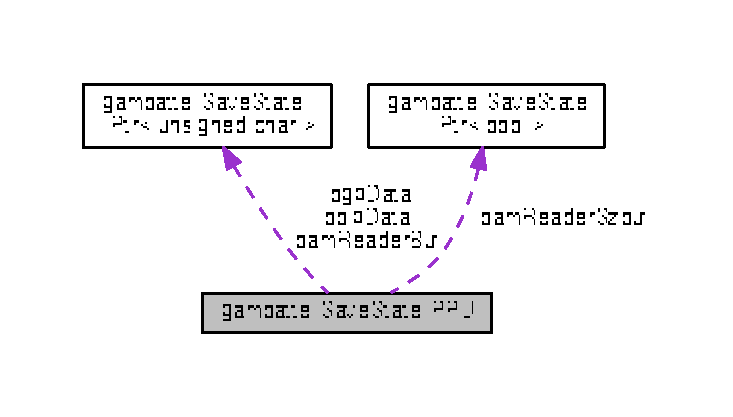
\includegraphics[width=350pt]{structgambatte_1_1SaveState_1_1PPU__coll__graph}
\end{center}
\end{figure}
\subsection*{Public Attributes}
\begin{DoxyCompactItemize}
\item 
\hyperlink{classgambatte_1_1SaveState_1_1Ptr}{Ptr}$<$ unsigned char $>$ \hyperlink{structgambatte_1_1SaveState_1_1PPU_aa76c0d6395f65bdfe6984b15c715ccdc}{bgp\+Data}
\item 
\hyperlink{classgambatte_1_1SaveState_1_1Ptr}{Ptr}$<$ unsigned char $>$ \hyperlink{structgambatte_1_1SaveState_1_1PPU_accaae5e4c05b6af8897b50767084d99c}{objp\+Data}
\item 
\hyperlink{classgambatte_1_1SaveState_1_1Ptr}{Ptr}$<$ unsigned char $>$ \hyperlink{structgambatte_1_1SaveState_1_1PPU_a07a06820413808bfc11ebb06d1ef2052}{oam\+Reader\+Buf}
\item 
\hyperlink{classgambatte_1_1SaveState_1_1Ptr}{Ptr}$<$ bool $>$ \hyperlink{structgambatte_1_1SaveState_1_1PPU_a1f41bd53d646bd6c5ed0bae3169c28fb}{oam\+Reader\+Szbuf}
\item 
unsigned \hyperlink{structgambatte_1_1SaveState_1_1PPU_a3c84cd6d28569d76001f0e2ec4bc5320}{video\+Cycles}
\item 
unsigned \hyperlink{structgambatte_1_1SaveState_1_1PPU_ae54e3b44537658fb80f8d75a2b653607}{enable\+Display\+M0\+Time}
\item 
unsigned short \hyperlink{structgambatte_1_1SaveState_1_1PPU_a54292ce6465993422fcb2a0151c4532c}{last\+M0\+Time}
\item 
unsigned short \hyperlink{structgambatte_1_1SaveState_1_1PPU_aabf33f08f8637993ef8c8ae9d15c3010}{next\+M0\+Irq}
\item 
unsigned short \hyperlink{structgambatte_1_1SaveState_1_1PPU_a33cc35ba7ac5d270121fe3bc1059f4e9}{tileword}
\item 
unsigned short \hyperlink{structgambatte_1_1SaveState_1_1PPU_ad8a9a6132afb9c6978f5fedb8627a093}{ntileword}
\item 
unsigned char \hyperlink{structgambatte_1_1SaveState_1_1PPU_ad5e4e377c6d8b48baa7473d5e0b7bdcb}{sp\+Attrib\+List} \mbox{[}10\mbox{]}
\item 
unsigned char \hyperlink{structgambatte_1_1SaveState_1_1PPU_a9b357530d61e861ff2b690be5023f353}{sp\+Byte0\+List} \mbox{[}10\mbox{]}
\item 
unsigned char \hyperlink{structgambatte_1_1SaveState_1_1PPU_a7611df8b8268ec5b522a7bc5c76f569e}{sp\+Byte1\+List} \mbox{[}10\mbox{]}
\item 
unsigned char \hyperlink{structgambatte_1_1SaveState_1_1PPU_abbc3b3a5d9961bcff5f1c58cb11099c7}{win\+Y\+Pos}
\item 
unsigned char \hyperlink{structgambatte_1_1SaveState_1_1PPU_a4cede5d88c31db884c02ec5547ae8ceb}{xpos}
\item 
unsigned char \hyperlink{structgambatte_1_1SaveState_1_1PPU_abe2c9145e622b8e99ff87ceedb8baeff}{endx}
\item 
unsigned char \hyperlink{structgambatte_1_1SaveState_1_1PPU_a84648df39d301ca942bc50a36dfe1dd3}{reg0}
\item 
unsigned char \hyperlink{structgambatte_1_1SaveState_1_1PPU_a8bd8169b9a763c17bd15c3c9c5866f0c}{reg1}
\item 
unsigned char \hyperlink{structgambatte_1_1SaveState_1_1PPU_a500021f50efc515f9bbf7cabd0a77a6b}{attrib}
\item 
unsigned char \hyperlink{structgambatte_1_1SaveState_1_1PPU_a8b27a2b9ab5953c02ba735ff5d7f197a}{nattrib}
\item 
unsigned char \hyperlink{structgambatte_1_1SaveState_1_1PPU_a2ad525914659c6e55440272352d20355}{state}
\item 
unsigned char \hyperlink{structgambatte_1_1SaveState_1_1PPU_a0188cf3be86c6b4338fcfea215089374}{next\+Sprite}
\item 
unsigned char \hyperlink{structgambatte_1_1SaveState_1_1PPU_a2a76d262159b270c5a3359bd8bef8fb3}{current\+Sprite}
\item 
unsigned char \hyperlink{structgambatte_1_1SaveState_1_1PPU_acb7f03d9e87fb73d89688ea2d8789abe}{lyc}
\item 
unsigned char \hyperlink{structgambatte_1_1SaveState_1_1PPU_a25f14433cb1ac9997c84af8fbfb51962}{m0lyc}
\item 
unsigned char \hyperlink{structgambatte_1_1SaveState_1_1PPU_a46bc471457cfdef2e53a362fb9929bf5}{old\+Wy}
\item 
unsigned char \hyperlink{structgambatte_1_1SaveState_1_1PPU_a465e410d70f2de41d140d313cfd9f5ac}{win\+Draw\+State}
\item 
unsigned char \hyperlink{structgambatte_1_1SaveState_1_1PPU_a28a408a0782d051ae7e298ea298112e3}{wscx}
\item 
bool \hyperlink{structgambatte_1_1SaveState_1_1PPU_a21367dcad642b246d4ffc41d1aed912c}{we\+Master}
\item 
bool \hyperlink{structgambatte_1_1SaveState_1_1PPU_af5cdde1c516c00f63d2eb4f0b1cb6040}{pending\+Lcdstat\+Irq}
\end{DoxyCompactItemize}


\subsection{Member Data Documentation}
\mbox{\Hypertarget{structgambatte_1_1SaveState_1_1PPU_a500021f50efc515f9bbf7cabd0a77a6b}\label{structgambatte_1_1SaveState_1_1PPU_a500021f50efc515f9bbf7cabd0a77a6b}} 
\index{gambatte\+::\+Save\+State\+::\+P\+PU@{gambatte\+::\+Save\+State\+::\+P\+PU}!attrib@{attrib}}
\index{attrib@{attrib}!gambatte\+::\+Save\+State\+::\+P\+PU@{gambatte\+::\+Save\+State\+::\+P\+PU}}
\subsubsection{\texorpdfstring{attrib}{attrib}}
{\footnotesize\ttfamily unsigned char gambatte\+::\+Save\+State\+::\+P\+P\+U\+::attrib}

\mbox{\Hypertarget{structgambatte_1_1SaveState_1_1PPU_aa76c0d6395f65bdfe6984b15c715ccdc}\label{structgambatte_1_1SaveState_1_1PPU_aa76c0d6395f65bdfe6984b15c715ccdc}} 
\index{gambatte\+::\+Save\+State\+::\+P\+PU@{gambatte\+::\+Save\+State\+::\+P\+PU}!bgp\+Data@{bgp\+Data}}
\index{bgp\+Data@{bgp\+Data}!gambatte\+::\+Save\+State\+::\+P\+PU@{gambatte\+::\+Save\+State\+::\+P\+PU}}
\subsubsection{\texorpdfstring{bgp\+Data}{bgpData}}
{\footnotesize\ttfamily \hyperlink{classgambatte_1_1SaveState_1_1Ptr}{Ptr}$<$unsigned char$>$ gambatte\+::\+Save\+State\+::\+P\+P\+U\+::bgp\+Data}

\mbox{\Hypertarget{structgambatte_1_1SaveState_1_1PPU_a2a76d262159b270c5a3359bd8bef8fb3}\label{structgambatte_1_1SaveState_1_1PPU_a2a76d262159b270c5a3359bd8bef8fb3}} 
\index{gambatte\+::\+Save\+State\+::\+P\+PU@{gambatte\+::\+Save\+State\+::\+P\+PU}!current\+Sprite@{current\+Sprite}}
\index{current\+Sprite@{current\+Sprite}!gambatte\+::\+Save\+State\+::\+P\+PU@{gambatte\+::\+Save\+State\+::\+P\+PU}}
\subsubsection{\texorpdfstring{current\+Sprite}{currentSprite}}
{\footnotesize\ttfamily unsigned char gambatte\+::\+Save\+State\+::\+P\+P\+U\+::current\+Sprite}

\mbox{\Hypertarget{structgambatte_1_1SaveState_1_1PPU_ae54e3b44537658fb80f8d75a2b653607}\label{structgambatte_1_1SaveState_1_1PPU_ae54e3b44537658fb80f8d75a2b653607}} 
\index{gambatte\+::\+Save\+State\+::\+P\+PU@{gambatte\+::\+Save\+State\+::\+P\+PU}!enable\+Display\+M0\+Time@{enable\+Display\+M0\+Time}}
\index{enable\+Display\+M0\+Time@{enable\+Display\+M0\+Time}!gambatte\+::\+Save\+State\+::\+P\+PU@{gambatte\+::\+Save\+State\+::\+P\+PU}}
\subsubsection{\texorpdfstring{enable\+Display\+M0\+Time}{enableDisplayM0Time}}
{\footnotesize\ttfamily unsigned gambatte\+::\+Save\+State\+::\+P\+P\+U\+::enable\+Display\+M0\+Time}

\mbox{\Hypertarget{structgambatte_1_1SaveState_1_1PPU_abe2c9145e622b8e99ff87ceedb8baeff}\label{structgambatte_1_1SaveState_1_1PPU_abe2c9145e622b8e99ff87ceedb8baeff}} 
\index{gambatte\+::\+Save\+State\+::\+P\+PU@{gambatte\+::\+Save\+State\+::\+P\+PU}!endx@{endx}}
\index{endx@{endx}!gambatte\+::\+Save\+State\+::\+P\+PU@{gambatte\+::\+Save\+State\+::\+P\+PU}}
\subsubsection{\texorpdfstring{endx}{endx}}
{\footnotesize\ttfamily unsigned char gambatte\+::\+Save\+State\+::\+P\+P\+U\+::endx}

\mbox{\Hypertarget{structgambatte_1_1SaveState_1_1PPU_a54292ce6465993422fcb2a0151c4532c}\label{structgambatte_1_1SaveState_1_1PPU_a54292ce6465993422fcb2a0151c4532c}} 
\index{gambatte\+::\+Save\+State\+::\+P\+PU@{gambatte\+::\+Save\+State\+::\+P\+PU}!last\+M0\+Time@{last\+M0\+Time}}
\index{last\+M0\+Time@{last\+M0\+Time}!gambatte\+::\+Save\+State\+::\+P\+PU@{gambatte\+::\+Save\+State\+::\+P\+PU}}
\subsubsection{\texorpdfstring{last\+M0\+Time}{lastM0Time}}
{\footnotesize\ttfamily unsigned short gambatte\+::\+Save\+State\+::\+P\+P\+U\+::last\+M0\+Time}

\mbox{\Hypertarget{structgambatte_1_1SaveState_1_1PPU_acb7f03d9e87fb73d89688ea2d8789abe}\label{structgambatte_1_1SaveState_1_1PPU_acb7f03d9e87fb73d89688ea2d8789abe}} 
\index{gambatte\+::\+Save\+State\+::\+P\+PU@{gambatte\+::\+Save\+State\+::\+P\+PU}!lyc@{lyc}}
\index{lyc@{lyc}!gambatte\+::\+Save\+State\+::\+P\+PU@{gambatte\+::\+Save\+State\+::\+P\+PU}}
\subsubsection{\texorpdfstring{lyc}{lyc}}
{\footnotesize\ttfamily unsigned char gambatte\+::\+Save\+State\+::\+P\+P\+U\+::lyc}

\mbox{\Hypertarget{structgambatte_1_1SaveState_1_1PPU_a25f14433cb1ac9997c84af8fbfb51962}\label{structgambatte_1_1SaveState_1_1PPU_a25f14433cb1ac9997c84af8fbfb51962}} 
\index{gambatte\+::\+Save\+State\+::\+P\+PU@{gambatte\+::\+Save\+State\+::\+P\+PU}!m0lyc@{m0lyc}}
\index{m0lyc@{m0lyc}!gambatte\+::\+Save\+State\+::\+P\+PU@{gambatte\+::\+Save\+State\+::\+P\+PU}}
\subsubsection{\texorpdfstring{m0lyc}{m0lyc}}
{\footnotesize\ttfamily unsigned char gambatte\+::\+Save\+State\+::\+P\+P\+U\+::m0lyc}

\mbox{\Hypertarget{structgambatte_1_1SaveState_1_1PPU_a8b27a2b9ab5953c02ba735ff5d7f197a}\label{structgambatte_1_1SaveState_1_1PPU_a8b27a2b9ab5953c02ba735ff5d7f197a}} 
\index{gambatte\+::\+Save\+State\+::\+P\+PU@{gambatte\+::\+Save\+State\+::\+P\+PU}!nattrib@{nattrib}}
\index{nattrib@{nattrib}!gambatte\+::\+Save\+State\+::\+P\+PU@{gambatte\+::\+Save\+State\+::\+P\+PU}}
\subsubsection{\texorpdfstring{nattrib}{nattrib}}
{\footnotesize\ttfamily unsigned char gambatte\+::\+Save\+State\+::\+P\+P\+U\+::nattrib}

\mbox{\Hypertarget{structgambatte_1_1SaveState_1_1PPU_aabf33f08f8637993ef8c8ae9d15c3010}\label{structgambatte_1_1SaveState_1_1PPU_aabf33f08f8637993ef8c8ae9d15c3010}} 
\index{gambatte\+::\+Save\+State\+::\+P\+PU@{gambatte\+::\+Save\+State\+::\+P\+PU}!next\+M0\+Irq@{next\+M0\+Irq}}
\index{next\+M0\+Irq@{next\+M0\+Irq}!gambatte\+::\+Save\+State\+::\+P\+PU@{gambatte\+::\+Save\+State\+::\+P\+PU}}
\subsubsection{\texorpdfstring{next\+M0\+Irq}{nextM0Irq}}
{\footnotesize\ttfamily unsigned short gambatte\+::\+Save\+State\+::\+P\+P\+U\+::next\+M0\+Irq}

\mbox{\Hypertarget{structgambatte_1_1SaveState_1_1PPU_a0188cf3be86c6b4338fcfea215089374}\label{structgambatte_1_1SaveState_1_1PPU_a0188cf3be86c6b4338fcfea215089374}} 
\index{gambatte\+::\+Save\+State\+::\+P\+PU@{gambatte\+::\+Save\+State\+::\+P\+PU}!next\+Sprite@{next\+Sprite}}
\index{next\+Sprite@{next\+Sprite}!gambatte\+::\+Save\+State\+::\+P\+PU@{gambatte\+::\+Save\+State\+::\+P\+PU}}
\subsubsection{\texorpdfstring{next\+Sprite}{nextSprite}}
{\footnotesize\ttfamily unsigned char gambatte\+::\+Save\+State\+::\+P\+P\+U\+::next\+Sprite}

\mbox{\Hypertarget{structgambatte_1_1SaveState_1_1PPU_ad8a9a6132afb9c6978f5fedb8627a093}\label{structgambatte_1_1SaveState_1_1PPU_ad8a9a6132afb9c6978f5fedb8627a093}} 
\index{gambatte\+::\+Save\+State\+::\+P\+PU@{gambatte\+::\+Save\+State\+::\+P\+PU}!ntileword@{ntileword}}
\index{ntileword@{ntileword}!gambatte\+::\+Save\+State\+::\+P\+PU@{gambatte\+::\+Save\+State\+::\+P\+PU}}
\subsubsection{\texorpdfstring{ntileword}{ntileword}}
{\footnotesize\ttfamily unsigned short gambatte\+::\+Save\+State\+::\+P\+P\+U\+::ntileword}

\mbox{\Hypertarget{structgambatte_1_1SaveState_1_1PPU_a07a06820413808bfc11ebb06d1ef2052}\label{structgambatte_1_1SaveState_1_1PPU_a07a06820413808bfc11ebb06d1ef2052}} 
\index{gambatte\+::\+Save\+State\+::\+P\+PU@{gambatte\+::\+Save\+State\+::\+P\+PU}!oam\+Reader\+Buf@{oam\+Reader\+Buf}}
\index{oam\+Reader\+Buf@{oam\+Reader\+Buf}!gambatte\+::\+Save\+State\+::\+P\+PU@{gambatte\+::\+Save\+State\+::\+P\+PU}}
\subsubsection{\texorpdfstring{oam\+Reader\+Buf}{oamReaderBuf}}
{\footnotesize\ttfamily \hyperlink{classgambatte_1_1SaveState_1_1Ptr}{Ptr}$<$unsigned char$>$ gambatte\+::\+Save\+State\+::\+P\+P\+U\+::oam\+Reader\+Buf}

\mbox{\Hypertarget{structgambatte_1_1SaveState_1_1PPU_a1f41bd53d646bd6c5ed0bae3169c28fb}\label{structgambatte_1_1SaveState_1_1PPU_a1f41bd53d646bd6c5ed0bae3169c28fb}} 
\index{gambatte\+::\+Save\+State\+::\+P\+PU@{gambatte\+::\+Save\+State\+::\+P\+PU}!oam\+Reader\+Szbuf@{oam\+Reader\+Szbuf}}
\index{oam\+Reader\+Szbuf@{oam\+Reader\+Szbuf}!gambatte\+::\+Save\+State\+::\+P\+PU@{gambatte\+::\+Save\+State\+::\+P\+PU}}
\subsubsection{\texorpdfstring{oam\+Reader\+Szbuf}{oamReaderSzbuf}}
{\footnotesize\ttfamily \hyperlink{classgambatte_1_1SaveState_1_1Ptr}{Ptr}$<$bool$>$ gambatte\+::\+Save\+State\+::\+P\+P\+U\+::oam\+Reader\+Szbuf}

\mbox{\Hypertarget{structgambatte_1_1SaveState_1_1PPU_accaae5e4c05b6af8897b50767084d99c}\label{structgambatte_1_1SaveState_1_1PPU_accaae5e4c05b6af8897b50767084d99c}} 
\index{gambatte\+::\+Save\+State\+::\+P\+PU@{gambatte\+::\+Save\+State\+::\+P\+PU}!objp\+Data@{objp\+Data}}
\index{objp\+Data@{objp\+Data}!gambatte\+::\+Save\+State\+::\+P\+PU@{gambatte\+::\+Save\+State\+::\+P\+PU}}
\subsubsection{\texorpdfstring{objp\+Data}{objpData}}
{\footnotesize\ttfamily \hyperlink{classgambatte_1_1SaveState_1_1Ptr}{Ptr}$<$unsigned char$>$ gambatte\+::\+Save\+State\+::\+P\+P\+U\+::objp\+Data}

\mbox{\Hypertarget{structgambatte_1_1SaveState_1_1PPU_a46bc471457cfdef2e53a362fb9929bf5}\label{structgambatte_1_1SaveState_1_1PPU_a46bc471457cfdef2e53a362fb9929bf5}} 
\index{gambatte\+::\+Save\+State\+::\+P\+PU@{gambatte\+::\+Save\+State\+::\+P\+PU}!old\+Wy@{old\+Wy}}
\index{old\+Wy@{old\+Wy}!gambatte\+::\+Save\+State\+::\+P\+PU@{gambatte\+::\+Save\+State\+::\+P\+PU}}
\subsubsection{\texorpdfstring{old\+Wy}{oldWy}}
{\footnotesize\ttfamily unsigned char gambatte\+::\+Save\+State\+::\+P\+P\+U\+::old\+Wy}

\mbox{\Hypertarget{structgambatte_1_1SaveState_1_1PPU_af5cdde1c516c00f63d2eb4f0b1cb6040}\label{structgambatte_1_1SaveState_1_1PPU_af5cdde1c516c00f63d2eb4f0b1cb6040}} 
\index{gambatte\+::\+Save\+State\+::\+P\+PU@{gambatte\+::\+Save\+State\+::\+P\+PU}!pending\+Lcdstat\+Irq@{pending\+Lcdstat\+Irq}}
\index{pending\+Lcdstat\+Irq@{pending\+Lcdstat\+Irq}!gambatte\+::\+Save\+State\+::\+P\+PU@{gambatte\+::\+Save\+State\+::\+P\+PU}}
\subsubsection{\texorpdfstring{pending\+Lcdstat\+Irq}{pendingLcdstatIrq}}
{\footnotesize\ttfamily bool gambatte\+::\+Save\+State\+::\+P\+P\+U\+::pending\+Lcdstat\+Irq}

\mbox{\Hypertarget{structgambatte_1_1SaveState_1_1PPU_a84648df39d301ca942bc50a36dfe1dd3}\label{structgambatte_1_1SaveState_1_1PPU_a84648df39d301ca942bc50a36dfe1dd3}} 
\index{gambatte\+::\+Save\+State\+::\+P\+PU@{gambatte\+::\+Save\+State\+::\+P\+PU}!reg0@{reg0}}
\index{reg0@{reg0}!gambatte\+::\+Save\+State\+::\+P\+PU@{gambatte\+::\+Save\+State\+::\+P\+PU}}
\subsubsection{\texorpdfstring{reg0}{reg0}}
{\footnotesize\ttfamily unsigned char gambatte\+::\+Save\+State\+::\+P\+P\+U\+::reg0}

\mbox{\Hypertarget{structgambatte_1_1SaveState_1_1PPU_a8bd8169b9a763c17bd15c3c9c5866f0c}\label{structgambatte_1_1SaveState_1_1PPU_a8bd8169b9a763c17bd15c3c9c5866f0c}} 
\index{gambatte\+::\+Save\+State\+::\+P\+PU@{gambatte\+::\+Save\+State\+::\+P\+PU}!reg1@{reg1}}
\index{reg1@{reg1}!gambatte\+::\+Save\+State\+::\+P\+PU@{gambatte\+::\+Save\+State\+::\+P\+PU}}
\subsubsection{\texorpdfstring{reg1}{reg1}}
{\footnotesize\ttfamily unsigned char gambatte\+::\+Save\+State\+::\+P\+P\+U\+::reg1}

\mbox{\Hypertarget{structgambatte_1_1SaveState_1_1PPU_ad5e4e377c6d8b48baa7473d5e0b7bdcb}\label{structgambatte_1_1SaveState_1_1PPU_ad5e4e377c6d8b48baa7473d5e0b7bdcb}} 
\index{gambatte\+::\+Save\+State\+::\+P\+PU@{gambatte\+::\+Save\+State\+::\+P\+PU}!sp\+Attrib\+List@{sp\+Attrib\+List}}
\index{sp\+Attrib\+List@{sp\+Attrib\+List}!gambatte\+::\+Save\+State\+::\+P\+PU@{gambatte\+::\+Save\+State\+::\+P\+PU}}
\subsubsection{\texorpdfstring{sp\+Attrib\+List}{spAttribList}}
{\footnotesize\ttfamily unsigned char gambatte\+::\+Save\+State\+::\+P\+P\+U\+::sp\+Attrib\+List\mbox{[}10\mbox{]}}

\mbox{\Hypertarget{structgambatte_1_1SaveState_1_1PPU_a9b357530d61e861ff2b690be5023f353}\label{structgambatte_1_1SaveState_1_1PPU_a9b357530d61e861ff2b690be5023f353}} 
\index{gambatte\+::\+Save\+State\+::\+P\+PU@{gambatte\+::\+Save\+State\+::\+P\+PU}!sp\+Byte0\+List@{sp\+Byte0\+List}}
\index{sp\+Byte0\+List@{sp\+Byte0\+List}!gambatte\+::\+Save\+State\+::\+P\+PU@{gambatte\+::\+Save\+State\+::\+P\+PU}}
\subsubsection{\texorpdfstring{sp\+Byte0\+List}{spByte0List}}
{\footnotesize\ttfamily unsigned char gambatte\+::\+Save\+State\+::\+P\+P\+U\+::sp\+Byte0\+List\mbox{[}10\mbox{]}}

\mbox{\Hypertarget{structgambatte_1_1SaveState_1_1PPU_a7611df8b8268ec5b522a7bc5c76f569e}\label{structgambatte_1_1SaveState_1_1PPU_a7611df8b8268ec5b522a7bc5c76f569e}} 
\index{gambatte\+::\+Save\+State\+::\+P\+PU@{gambatte\+::\+Save\+State\+::\+P\+PU}!sp\+Byte1\+List@{sp\+Byte1\+List}}
\index{sp\+Byte1\+List@{sp\+Byte1\+List}!gambatte\+::\+Save\+State\+::\+P\+PU@{gambatte\+::\+Save\+State\+::\+P\+PU}}
\subsubsection{\texorpdfstring{sp\+Byte1\+List}{spByte1List}}
{\footnotesize\ttfamily unsigned char gambatte\+::\+Save\+State\+::\+P\+P\+U\+::sp\+Byte1\+List\mbox{[}10\mbox{]}}

\mbox{\Hypertarget{structgambatte_1_1SaveState_1_1PPU_a2ad525914659c6e55440272352d20355}\label{structgambatte_1_1SaveState_1_1PPU_a2ad525914659c6e55440272352d20355}} 
\index{gambatte\+::\+Save\+State\+::\+P\+PU@{gambatte\+::\+Save\+State\+::\+P\+PU}!state@{state}}
\index{state@{state}!gambatte\+::\+Save\+State\+::\+P\+PU@{gambatte\+::\+Save\+State\+::\+P\+PU}}
\subsubsection{\texorpdfstring{state}{state}}
{\footnotesize\ttfamily unsigned char gambatte\+::\+Save\+State\+::\+P\+P\+U\+::state}

\mbox{\Hypertarget{structgambatte_1_1SaveState_1_1PPU_a33cc35ba7ac5d270121fe3bc1059f4e9}\label{structgambatte_1_1SaveState_1_1PPU_a33cc35ba7ac5d270121fe3bc1059f4e9}} 
\index{gambatte\+::\+Save\+State\+::\+P\+PU@{gambatte\+::\+Save\+State\+::\+P\+PU}!tileword@{tileword}}
\index{tileword@{tileword}!gambatte\+::\+Save\+State\+::\+P\+PU@{gambatte\+::\+Save\+State\+::\+P\+PU}}
\subsubsection{\texorpdfstring{tileword}{tileword}}
{\footnotesize\ttfamily unsigned short gambatte\+::\+Save\+State\+::\+P\+P\+U\+::tileword}

\mbox{\Hypertarget{structgambatte_1_1SaveState_1_1PPU_a3c84cd6d28569d76001f0e2ec4bc5320}\label{structgambatte_1_1SaveState_1_1PPU_a3c84cd6d28569d76001f0e2ec4bc5320}} 
\index{gambatte\+::\+Save\+State\+::\+P\+PU@{gambatte\+::\+Save\+State\+::\+P\+PU}!video\+Cycles@{video\+Cycles}}
\index{video\+Cycles@{video\+Cycles}!gambatte\+::\+Save\+State\+::\+P\+PU@{gambatte\+::\+Save\+State\+::\+P\+PU}}
\subsubsection{\texorpdfstring{video\+Cycles}{videoCycles}}
{\footnotesize\ttfamily unsigned gambatte\+::\+Save\+State\+::\+P\+P\+U\+::video\+Cycles}

\mbox{\Hypertarget{structgambatte_1_1SaveState_1_1PPU_a21367dcad642b246d4ffc41d1aed912c}\label{structgambatte_1_1SaveState_1_1PPU_a21367dcad642b246d4ffc41d1aed912c}} 
\index{gambatte\+::\+Save\+State\+::\+P\+PU@{gambatte\+::\+Save\+State\+::\+P\+PU}!we\+Master@{we\+Master}}
\index{we\+Master@{we\+Master}!gambatte\+::\+Save\+State\+::\+P\+PU@{gambatte\+::\+Save\+State\+::\+P\+PU}}
\subsubsection{\texorpdfstring{we\+Master}{weMaster}}
{\footnotesize\ttfamily bool gambatte\+::\+Save\+State\+::\+P\+P\+U\+::we\+Master}

\mbox{\Hypertarget{structgambatte_1_1SaveState_1_1PPU_a465e410d70f2de41d140d313cfd9f5ac}\label{structgambatte_1_1SaveState_1_1PPU_a465e410d70f2de41d140d313cfd9f5ac}} 
\index{gambatte\+::\+Save\+State\+::\+P\+PU@{gambatte\+::\+Save\+State\+::\+P\+PU}!win\+Draw\+State@{win\+Draw\+State}}
\index{win\+Draw\+State@{win\+Draw\+State}!gambatte\+::\+Save\+State\+::\+P\+PU@{gambatte\+::\+Save\+State\+::\+P\+PU}}
\subsubsection{\texorpdfstring{win\+Draw\+State}{winDrawState}}
{\footnotesize\ttfamily unsigned char gambatte\+::\+Save\+State\+::\+P\+P\+U\+::win\+Draw\+State}

\mbox{\Hypertarget{structgambatte_1_1SaveState_1_1PPU_abbc3b3a5d9961bcff5f1c58cb11099c7}\label{structgambatte_1_1SaveState_1_1PPU_abbc3b3a5d9961bcff5f1c58cb11099c7}} 
\index{gambatte\+::\+Save\+State\+::\+P\+PU@{gambatte\+::\+Save\+State\+::\+P\+PU}!win\+Y\+Pos@{win\+Y\+Pos}}
\index{win\+Y\+Pos@{win\+Y\+Pos}!gambatte\+::\+Save\+State\+::\+P\+PU@{gambatte\+::\+Save\+State\+::\+P\+PU}}
\subsubsection{\texorpdfstring{win\+Y\+Pos}{winYPos}}
{\footnotesize\ttfamily unsigned char gambatte\+::\+Save\+State\+::\+P\+P\+U\+::win\+Y\+Pos}

\mbox{\Hypertarget{structgambatte_1_1SaveState_1_1PPU_a28a408a0782d051ae7e298ea298112e3}\label{structgambatte_1_1SaveState_1_1PPU_a28a408a0782d051ae7e298ea298112e3}} 
\index{gambatte\+::\+Save\+State\+::\+P\+PU@{gambatte\+::\+Save\+State\+::\+P\+PU}!wscx@{wscx}}
\index{wscx@{wscx}!gambatte\+::\+Save\+State\+::\+P\+PU@{gambatte\+::\+Save\+State\+::\+P\+PU}}
\subsubsection{\texorpdfstring{wscx}{wscx}}
{\footnotesize\ttfamily unsigned char gambatte\+::\+Save\+State\+::\+P\+P\+U\+::wscx}

\mbox{\Hypertarget{structgambatte_1_1SaveState_1_1PPU_a4cede5d88c31db884c02ec5547ae8ceb}\label{structgambatte_1_1SaveState_1_1PPU_a4cede5d88c31db884c02ec5547ae8ceb}} 
\index{gambatte\+::\+Save\+State\+::\+P\+PU@{gambatte\+::\+Save\+State\+::\+P\+PU}!xpos@{xpos}}
\index{xpos@{xpos}!gambatte\+::\+Save\+State\+::\+P\+PU@{gambatte\+::\+Save\+State\+::\+P\+PU}}
\subsubsection{\texorpdfstring{xpos}{xpos}}
{\footnotesize\ttfamily unsigned char gambatte\+::\+Save\+State\+::\+P\+P\+U\+::xpos}



The documentation for this struct was generated from the following file\+:\begin{DoxyCompactItemize}
\item 
src/\hyperlink{savestate_8h}{savestate.\+h}\end{DoxyCompactItemize}

\hypertarget{classgambatte_1_1PPU}{}\section{gambatte\+:\+:P\+PU Class Reference}
\label{classgambatte_1_1PPU}\index{gambatte\+::\+P\+PU@{gambatte\+::\+P\+PU}}


{\ttfamily \#include $<$ppu.\+h$>$}



Collaboration diagram for gambatte\+:\+:P\+PU\+:
\nopagebreak
\begin{figure}[H]
\begin{center}
\leavevmode
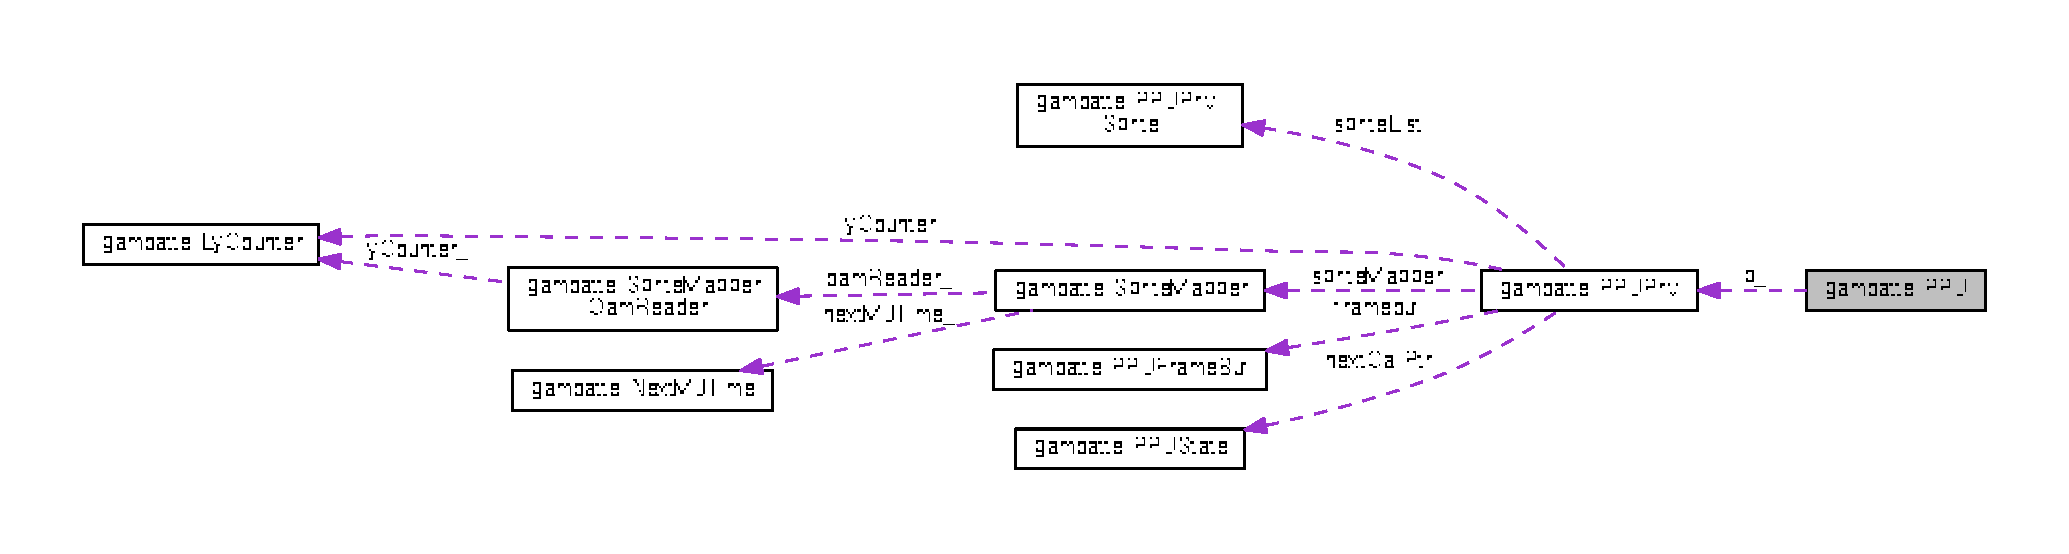
\includegraphics[width=350pt]{classgambatte_1_1PPU__coll__graph}
\end{center}
\end{figure}
\subsection*{Public Member Functions}
\begin{DoxyCompactItemize}
\item 
\hyperlink{classgambatte_1_1PPU_a9bd9298e9039c03f51781751d5651cc5}{P\+PU} (\hyperlink{classgambatte_1_1NextM0Time}{Next\+M0\+Time} \&next\+M0\+Time, unsigned char const $\ast$oamram, unsigned char const $\ast$vram)
\item 
\hyperlink{namespacegambatte_a0639f09fccfbbd5a8e0796318768e370}{uint\+\_\+least32\+\_\+t} $\ast$ \hyperlink{classgambatte_1_1PPU_ae81c3ac72e66573b86cc35cec0971482}{bg\+Palette} ()
\item 
bool \hyperlink{classgambatte_1_1PPU_a2753f1ba5217fe22bc0d518b63784825}{cgb} () const
\item 
void \hyperlink{classgambatte_1_1PPU_a283036ab67e35f5687410f131d5170e8}{do\+Ly\+Count\+Event} ()
\item 
unsigned \hyperlink{classgambatte_1_1PPU_a415ef4d53cac6e35dfa9d45650d7ddd0}{do\+Sprite\+Map\+Event} (unsigned time)
\item 
\hyperlink{classgambatte_1_1PPUFrameBuf}{P\+P\+U\+Frame\+Buf} const  \& \hyperlink{classgambatte_1_1PPU_a096a8908b52cfde8d8064b2fde06c1c0}{frame\+Buf} () const
\item 
bool \hyperlink{classgambatte_1_1PPU_aef091fcf827b99f11876f3dc8752ddbc}{inactive\+Period\+After\+Display\+Enable} (unsigned cc) const
\item 
unsigned \hyperlink{classgambatte_1_1PPU_a042e5d2be95bc598fbc0e2114c1540f7}{last\+M0\+Time} () const
\item 
unsigned \hyperlink{classgambatte_1_1PPU_aaafd3c2cf72649e5b144bb2ae6d2457a}{lcdc} () const
\item 
void \hyperlink{classgambatte_1_1PPU_a1b606146dff60d13acd0a5d860b910a1}{load\+State} (\hyperlink{structgambatte_1_1SaveState}{Save\+State} const \&\hyperlink{ppu_8cpp_a2f2eca6997ee7baf8901725ae074d45b}{state}, unsigned char const $\ast$oamram)
\item 
\hyperlink{classgambatte_1_1LyCounter}{Ly\+Counter} const  \& \hyperlink{classgambatte_1_1PPU_ae6bb249f7d93eb7ef39b44f9f398d194}{ly\+Counter} () const
\item 
unsigned \hyperlink{classgambatte_1_1PPU_aeeea3c335760b8f386059c144508e011}{now} () const
\item 
void \hyperlink{classgambatte_1_1PPU_ace3683a992aace437ce28239f43e7ab4}{oam\+Change} (unsigned cc)
\item 
void \hyperlink{classgambatte_1_1PPU_a5c1f4b8784c8303e0f3af5bbc27751a5}{oam\+Change} (unsigned char const $\ast$oamram, unsigned cc)
\item 
unsigned \hyperlink{classgambatte_1_1PPU_ad8d55b06d78e952bed556cf3e51c0b78}{predicted\+Next\+Xpos\+Time} (unsigned xpos) const
\item 
void \hyperlink{classgambatte_1_1PPU_a99cf75af19c1fca9c8464ed8f49e799d}{reset} (unsigned char const $\ast$oamram, unsigned char const $\ast$vram, bool \hyperlink{classgambatte_1_1PPU_a2753f1ba5217fe22bc0d518b63784825}{cgb})
\item 
void \hyperlink{classgambatte_1_1PPU_a43601e1b8576bcf31b9716bc2637d1cd}{reset\+Cc} (unsigned old\+Cc, unsigned new\+Cc)
\item 
void \hyperlink{classgambatte_1_1PPU_a56bea94c1f2c2caaa597145a3f95b01b}{save\+State} (\hyperlink{structgambatte_1_1SaveState}{Save\+State} \&ss) const
\item 
void \hyperlink{classgambatte_1_1PPU_a17571a5f4163a66bbc8310dca6c734aa}{flip\+Display} (\hyperlink{namespacegambatte_a0639f09fccfbbd5a8e0796318768e370}{uint\+\_\+least32\+\_\+t} $\ast$\hyperlink{ioapi_8h_a8ad8a13c88886b9f623034ff88570adb}{buf}, unsigned pitch)
\item 
void \hyperlink{classgambatte_1_1PPU_acf0e51190d5b912a91d9e9b8cbb1f8aa}{set\+Lcdc} (unsigned \hyperlink{classgambatte_1_1PPU_aaafd3c2cf72649e5b144bb2ae6d2457a}{lcdc}, unsigned cc)
\item 
void \hyperlink{classgambatte_1_1PPU_aae64d6ecf523571757b951632d783232}{set\+Scx} (unsigned scx)
\item 
void \hyperlink{classgambatte_1_1PPU_a277558e3f602884db0207063034e0c9b}{set\+Scy} (unsigned scy)
\item 
void \hyperlink{classgambatte_1_1PPU_a460be85dec82811e994a7cbb44a183e2}{set\+State\+Ptrs} (\hyperlink{structgambatte_1_1SaveState}{Save\+State} \&ss)
\item 
void \hyperlink{classgambatte_1_1PPU_a21c837eecefb1f260795c8894f7cbd0c}{set\+Wx} (unsigned wx)
\item 
void \hyperlink{classgambatte_1_1PPU_ab570e79665e77e73bab93985acd15d23}{set\+Wy} (unsigned wy)
\item 
void \hyperlink{classgambatte_1_1PPU_a33dbb53f8dc14f9a590777084f55d78c}{update\+Wy2} ()
\item 
void \hyperlink{classgambatte_1_1PPU_a8e075cf376f246914ceb768585fbfbf6}{speed\+Change} (unsigned cycle\+Counter)
\item 
\hyperlink{namespacegambatte_a0639f09fccfbbd5a8e0796318768e370}{uint\+\_\+least32\+\_\+t} $\ast$ \hyperlink{classgambatte_1_1PPU_ae6a6686a0751e14ff4f6cd794c6aada4}{sp\+Palette} ()
\item 
void \hyperlink{classgambatte_1_1PPU_a0ac64d34f6537dd249f30567d0a1b593}{update} (unsigned cc)
\item 
void \hyperlink{classgambatte_1_1PPU_a09d8a46b05a01daf4accbef11560d937}{load\+Or\+Save} (\hyperlink{classgambatte_1_1loadsave}{loadsave} \&\hyperlink{ppu_8cpp_a2f2eca6997ee7baf8901725ae074d45b}{state})
\end{DoxyCompactItemize}
\subsection*{Private Attributes}
\begin{DoxyCompactItemize}
\item 
\hyperlink{structgambatte_1_1PPUPriv}{P\+P\+U\+Priv} \hyperlink{classgambatte_1_1PPU_a125f5c1050b1e30ba0da55dfe1fc121b}{p\+\_\+}
\end{DoxyCompactItemize}


\subsection{Constructor \& Destructor Documentation}
\mbox{\Hypertarget{classgambatte_1_1PPU_a9bd9298e9039c03f51781751d5651cc5}\label{classgambatte_1_1PPU_a9bd9298e9039c03f51781751d5651cc5}} 
\index{gambatte\+::\+P\+PU@{gambatte\+::\+P\+PU}!P\+PU@{P\+PU}}
\index{P\+PU@{P\+PU}!gambatte\+::\+P\+PU@{gambatte\+::\+P\+PU}}
\subsubsection{\texorpdfstring{P\+P\+U()}{PPU()}}
{\footnotesize\ttfamily gambatte\+::\+P\+P\+U\+::\+P\+PU (\begin{DoxyParamCaption}\item[{\hyperlink{classgambatte_1_1NextM0Time}{Next\+M0\+Time} \&}]{next\+M0\+Time,  }\item[{unsigned char const $\ast$}]{oamram,  }\item[{unsigned char const $\ast$}]{vram }\end{DoxyParamCaption})\hspace{0.3cm}{\ttfamily [inline]}}



\subsection{Member Function Documentation}
\mbox{\Hypertarget{classgambatte_1_1PPU_ae81c3ac72e66573b86cc35cec0971482}\label{classgambatte_1_1PPU_ae81c3ac72e66573b86cc35cec0971482}} 
\index{gambatte\+::\+P\+PU@{gambatte\+::\+P\+PU}!bg\+Palette@{bg\+Palette}}
\index{bg\+Palette@{bg\+Palette}!gambatte\+::\+P\+PU@{gambatte\+::\+P\+PU}}
\subsubsection{\texorpdfstring{bg\+Palette()}{bgPalette()}}
{\footnotesize\ttfamily \hyperlink{namespacegambatte_a0639f09fccfbbd5a8e0796318768e370}{uint\+\_\+least32\+\_\+t}$\ast$ gambatte\+::\+P\+P\+U\+::bg\+Palette (\begin{DoxyParamCaption}{ }\end{DoxyParamCaption})\hspace{0.3cm}{\ttfamily [inline]}}

\mbox{\Hypertarget{classgambatte_1_1PPU_a2753f1ba5217fe22bc0d518b63784825}\label{classgambatte_1_1PPU_a2753f1ba5217fe22bc0d518b63784825}} 
\index{gambatte\+::\+P\+PU@{gambatte\+::\+P\+PU}!cgb@{cgb}}
\index{cgb@{cgb}!gambatte\+::\+P\+PU@{gambatte\+::\+P\+PU}}
\subsubsection{\texorpdfstring{cgb()}{cgb()}}
{\footnotesize\ttfamily bool gambatte\+::\+P\+P\+U\+::cgb (\begin{DoxyParamCaption}{ }\end{DoxyParamCaption}) const\hspace{0.3cm}{\ttfamily [inline]}}

\mbox{\Hypertarget{classgambatte_1_1PPU_a283036ab67e35f5687410f131d5170e8}\label{classgambatte_1_1PPU_a283036ab67e35f5687410f131d5170e8}} 
\index{gambatte\+::\+P\+PU@{gambatte\+::\+P\+PU}!do\+Ly\+Count\+Event@{do\+Ly\+Count\+Event}}
\index{do\+Ly\+Count\+Event@{do\+Ly\+Count\+Event}!gambatte\+::\+P\+PU@{gambatte\+::\+P\+PU}}
\subsubsection{\texorpdfstring{do\+Ly\+Count\+Event()}{doLyCountEvent()}}
{\footnotesize\ttfamily void gambatte\+::\+P\+P\+U\+::do\+Ly\+Count\+Event (\begin{DoxyParamCaption}{ }\end{DoxyParamCaption})\hspace{0.3cm}{\ttfamily [inline]}}

\mbox{\Hypertarget{classgambatte_1_1PPU_a415ef4d53cac6e35dfa9d45650d7ddd0}\label{classgambatte_1_1PPU_a415ef4d53cac6e35dfa9d45650d7ddd0}} 
\index{gambatte\+::\+P\+PU@{gambatte\+::\+P\+PU}!do\+Sprite\+Map\+Event@{do\+Sprite\+Map\+Event}}
\index{do\+Sprite\+Map\+Event@{do\+Sprite\+Map\+Event}!gambatte\+::\+P\+PU@{gambatte\+::\+P\+PU}}
\subsubsection{\texorpdfstring{do\+Sprite\+Map\+Event()}{doSpriteMapEvent()}}
{\footnotesize\ttfamily unsigned gambatte\+::\+P\+P\+U\+::do\+Sprite\+Map\+Event (\begin{DoxyParamCaption}\item[{unsigned}]{time }\end{DoxyParamCaption})\hspace{0.3cm}{\ttfamily [inline]}}

\mbox{\Hypertarget{classgambatte_1_1PPU_a17571a5f4163a66bbc8310dca6c734aa}\label{classgambatte_1_1PPU_a17571a5f4163a66bbc8310dca6c734aa}} 
\index{gambatte\+::\+P\+PU@{gambatte\+::\+P\+PU}!flip\+Display@{flip\+Display}}
\index{flip\+Display@{flip\+Display}!gambatte\+::\+P\+PU@{gambatte\+::\+P\+PU}}
\subsubsection{\texorpdfstring{flip\+Display()}{flipDisplay()}}
{\footnotesize\ttfamily void gambatte\+::\+P\+P\+U\+::flip\+Display (\begin{DoxyParamCaption}\item[{\hyperlink{namespacegambatte_a0639f09fccfbbd5a8e0796318768e370}{uint\+\_\+least32\+\_\+t} $\ast$}]{buf,  }\item[{unsigned}]{pitch }\end{DoxyParamCaption})\hspace{0.3cm}{\ttfamily [inline]}}

\mbox{\Hypertarget{classgambatte_1_1PPU_a096a8908b52cfde8d8064b2fde06c1c0}\label{classgambatte_1_1PPU_a096a8908b52cfde8d8064b2fde06c1c0}} 
\index{gambatte\+::\+P\+PU@{gambatte\+::\+P\+PU}!frame\+Buf@{frame\+Buf}}
\index{frame\+Buf@{frame\+Buf}!gambatte\+::\+P\+PU@{gambatte\+::\+P\+PU}}
\subsubsection{\texorpdfstring{frame\+Buf()}{frameBuf()}}
{\footnotesize\ttfamily \hyperlink{classgambatte_1_1PPUFrameBuf}{P\+P\+U\+Frame\+Buf} const\& gambatte\+::\+P\+P\+U\+::frame\+Buf (\begin{DoxyParamCaption}{ }\end{DoxyParamCaption}) const\hspace{0.3cm}{\ttfamily [inline]}}

\mbox{\Hypertarget{classgambatte_1_1PPU_aef091fcf827b99f11876f3dc8752ddbc}\label{classgambatte_1_1PPU_aef091fcf827b99f11876f3dc8752ddbc}} 
\index{gambatte\+::\+P\+PU@{gambatte\+::\+P\+PU}!inactive\+Period\+After\+Display\+Enable@{inactive\+Period\+After\+Display\+Enable}}
\index{inactive\+Period\+After\+Display\+Enable@{inactive\+Period\+After\+Display\+Enable}!gambatte\+::\+P\+PU@{gambatte\+::\+P\+PU}}
\subsubsection{\texorpdfstring{inactive\+Period\+After\+Display\+Enable()}{inactivePeriodAfterDisplayEnable()}}
{\footnotesize\ttfamily bool gambatte\+::\+P\+P\+U\+::inactive\+Period\+After\+Display\+Enable (\begin{DoxyParamCaption}\item[{unsigned}]{cc }\end{DoxyParamCaption}) const\hspace{0.3cm}{\ttfamily [inline]}}

\mbox{\Hypertarget{classgambatte_1_1PPU_a042e5d2be95bc598fbc0e2114c1540f7}\label{classgambatte_1_1PPU_a042e5d2be95bc598fbc0e2114c1540f7}} 
\index{gambatte\+::\+P\+PU@{gambatte\+::\+P\+PU}!last\+M0\+Time@{last\+M0\+Time}}
\index{last\+M0\+Time@{last\+M0\+Time}!gambatte\+::\+P\+PU@{gambatte\+::\+P\+PU}}
\subsubsection{\texorpdfstring{last\+M0\+Time()}{lastM0Time()}}
{\footnotesize\ttfamily unsigned gambatte\+::\+P\+P\+U\+::last\+M0\+Time (\begin{DoxyParamCaption}{ }\end{DoxyParamCaption}) const\hspace{0.3cm}{\ttfamily [inline]}}

\mbox{\Hypertarget{classgambatte_1_1PPU_aaafd3c2cf72649e5b144bb2ae6d2457a}\label{classgambatte_1_1PPU_aaafd3c2cf72649e5b144bb2ae6d2457a}} 
\index{gambatte\+::\+P\+PU@{gambatte\+::\+P\+PU}!lcdc@{lcdc}}
\index{lcdc@{lcdc}!gambatte\+::\+P\+PU@{gambatte\+::\+P\+PU}}
\subsubsection{\texorpdfstring{lcdc()}{lcdc()}}
{\footnotesize\ttfamily unsigned gambatte\+::\+P\+P\+U\+::lcdc (\begin{DoxyParamCaption}{ }\end{DoxyParamCaption}) const\hspace{0.3cm}{\ttfamily [inline]}}

\mbox{\Hypertarget{classgambatte_1_1PPU_a09d8a46b05a01daf4accbef11560d937}\label{classgambatte_1_1PPU_a09d8a46b05a01daf4accbef11560d937}} 
\index{gambatte\+::\+P\+PU@{gambatte\+::\+P\+PU}!load\+Or\+Save@{load\+Or\+Save}}
\index{load\+Or\+Save@{load\+Or\+Save}!gambatte\+::\+P\+PU@{gambatte\+::\+P\+PU}}
\subsubsection{\texorpdfstring{load\+Or\+Save()}{loadOrSave()}}
{\footnotesize\ttfamily void gambatte\+::\+P\+P\+U\+::load\+Or\+Save (\begin{DoxyParamCaption}\item[{\hyperlink{classgambatte_1_1loadsave}{loadsave} \&}]{state }\end{DoxyParamCaption})\hspace{0.3cm}{\ttfamily [inline]}}

\mbox{\Hypertarget{classgambatte_1_1PPU_a1b606146dff60d13acd0a5d860b910a1}\label{classgambatte_1_1PPU_a1b606146dff60d13acd0a5d860b910a1}} 
\index{gambatte\+::\+P\+PU@{gambatte\+::\+P\+PU}!load\+State@{load\+State}}
\index{load\+State@{load\+State}!gambatte\+::\+P\+PU@{gambatte\+::\+P\+PU}}
\subsubsection{\texorpdfstring{load\+State()}{loadState()}}
{\footnotesize\ttfamily void gambatte\+::\+P\+P\+U\+::load\+State (\begin{DoxyParamCaption}\item[{\hyperlink{structgambatte_1_1SaveState}{Save\+State} const \&}]{state,  }\item[{unsigned char const $\ast$}]{oamram }\end{DoxyParamCaption})}

\mbox{\Hypertarget{classgambatte_1_1PPU_ae6bb249f7d93eb7ef39b44f9f398d194}\label{classgambatte_1_1PPU_ae6bb249f7d93eb7ef39b44f9f398d194}} 
\index{gambatte\+::\+P\+PU@{gambatte\+::\+P\+PU}!ly\+Counter@{ly\+Counter}}
\index{ly\+Counter@{ly\+Counter}!gambatte\+::\+P\+PU@{gambatte\+::\+P\+PU}}
\subsubsection{\texorpdfstring{ly\+Counter()}{lyCounter()}}
{\footnotesize\ttfamily \hyperlink{classgambatte_1_1LyCounter}{Ly\+Counter} const\& gambatte\+::\+P\+P\+U\+::ly\+Counter (\begin{DoxyParamCaption}{ }\end{DoxyParamCaption}) const\hspace{0.3cm}{\ttfamily [inline]}}

\mbox{\Hypertarget{classgambatte_1_1PPU_aeeea3c335760b8f386059c144508e011}\label{classgambatte_1_1PPU_aeeea3c335760b8f386059c144508e011}} 
\index{gambatte\+::\+P\+PU@{gambatte\+::\+P\+PU}!now@{now}}
\index{now@{now}!gambatte\+::\+P\+PU@{gambatte\+::\+P\+PU}}
\subsubsection{\texorpdfstring{now()}{now()}}
{\footnotesize\ttfamily unsigned gambatte\+::\+P\+P\+U\+::now (\begin{DoxyParamCaption}{ }\end{DoxyParamCaption}) const\hspace{0.3cm}{\ttfamily [inline]}}

\mbox{\Hypertarget{classgambatte_1_1PPU_ace3683a992aace437ce28239f43e7ab4}\label{classgambatte_1_1PPU_ace3683a992aace437ce28239f43e7ab4}} 
\index{gambatte\+::\+P\+PU@{gambatte\+::\+P\+PU}!oam\+Change@{oam\+Change}}
\index{oam\+Change@{oam\+Change}!gambatte\+::\+P\+PU@{gambatte\+::\+P\+PU}}
\subsubsection{\texorpdfstring{oam\+Change()}{oamChange()}\hspace{0.1cm}{\footnotesize\ttfamily [1/2]}}
{\footnotesize\ttfamily void gambatte\+::\+P\+P\+U\+::oam\+Change (\begin{DoxyParamCaption}\item[{unsigned}]{cc }\end{DoxyParamCaption})\hspace{0.3cm}{\ttfamily [inline]}}

\mbox{\Hypertarget{classgambatte_1_1PPU_a5c1f4b8784c8303e0f3af5bbc27751a5}\label{classgambatte_1_1PPU_a5c1f4b8784c8303e0f3af5bbc27751a5}} 
\index{gambatte\+::\+P\+PU@{gambatte\+::\+P\+PU}!oam\+Change@{oam\+Change}}
\index{oam\+Change@{oam\+Change}!gambatte\+::\+P\+PU@{gambatte\+::\+P\+PU}}
\subsubsection{\texorpdfstring{oam\+Change()}{oamChange()}\hspace{0.1cm}{\footnotesize\ttfamily [2/2]}}
{\footnotesize\ttfamily void gambatte\+::\+P\+P\+U\+::oam\+Change (\begin{DoxyParamCaption}\item[{unsigned char const $\ast$}]{oamram,  }\item[{unsigned}]{cc }\end{DoxyParamCaption})\hspace{0.3cm}{\ttfamily [inline]}}

\mbox{\Hypertarget{classgambatte_1_1PPU_ad8d55b06d78e952bed556cf3e51c0b78}\label{classgambatte_1_1PPU_ad8d55b06d78e952bed556cf3e51c0b78}} 
\index{gambatte\+::\+P\+PU@{gambatte\+::\+P\+PU}!predicted\+Next\+Xpos\+Time@{predicted\+Next\+Xpos\+Time}}
\index{predicted\+Next\+Xpos\+Time@{predicted\+Next\+Xpos\+Time}!gambatte\+::\+P\+PU@{gambatte\+::\+P\+PU}}
\subsubsection{\texorpdfstring{predicted\+Next\+Xpos\+Time()}{predictedNextXposTime()}}
{\footnotesize\ttfamily unsigned gambatte\+::\+P\+P\+U\+::predicted\+Next\+Xpos\+Time (\begin{DoxyParamCaption}\item[{unsigned}]{xpos }\end{DoxyParamCaption}) const}

\mbox{\Hypertarget{classgambatte_1_1PPU_a99cf75af19c1fca9c8464ed8f49e799d}\label{classgambatte_1_1PPU_a99cf75af19c1fca9c8464ed8f49e799d}} 
\index{gambatte\+::\+P\+PU@{gambatte\+::\+P\+PU}!reset@{reset}}
\index{reset@{reset}!gambatte\+::\+P\+PU@{gambatte\+::\+P\+PU}}
\subsubsection{\texorpdfstring{reset()}{reset()}}
{\footnotesize\ttfamily void gambatte\+::\+P\+P\+U\+::reset (\begin{DoxyParamCaption}\item[{unsigned char const $\ast$}]{oamram,  }\item[{unsigned char const $\ast$}]{vram,  }\item[{bool}]{cgb }\end{DoxyParamCaption})}

\mbox{\Hypertarget{classgambatte_1_1PPU_a43601e1b8576bcf31b9716bc2637d1cd}\label{classgambatte_1_1PPU_a43601e1b8576bcf31b9716bc2637d1cd}} 
\index{gambatte\+::\+P\+PU@{gambatte\+::\+P\+PU}!reset\+Cc@{reset\+Cc}}
\index{reset\+Cc@{reset\+Cc}!gambatte\+::\+P\+PU@{gambatte\+::\+P\+PU}}
\subsubsection{\texorpdfstring{reset\+Cc()}{resetCc()}}
{\footnotesize\ttfamily void gambatte\+::\+P\+P\+U\+::reset\+Cc (\begin{DoxyParamCaption}\item[{unsigned}]{old\+Cc,  }\item[{unsigned}]{new\+Cc }\end{DoxyParamCaption})}

\mbox{\Hypertarget{classgambatte_1_1PPU_a56bea94c1f2c2caaa597145a3f95b01b}\label{classgambatte_1_1PPU_a56bea94c1f2c2caaa597145a3f95b01b}} 
\index{gambatte\+::\+P\+PU@{gambatte\+::\+P\+PU}!save\+State@{save\+State}}
\index{save\+State@{save\+State}!gambatte\+::\+P\+PU@{gambatte\+::\+P\+PU}}
\subsubsection{\texorpdfstring{save\+State()}{saveState()}}
{\footnotesize\ttfamily void gambatte\+::\+P\+P\+U\+::save\+State (\begin{DoxyParamCaption}\item[{\hyperlink{structgambatte_1_1SaveState}{Save\+State} \&}]{ss }\end{DoxyParamCaption}) const}

\mbox{\Hypertarget{classgambatte_1_1PPU_acf0e51190d5b912a91d9e9b8cbb1f8aa}\label{classgambatte_1_1PPU_acf0e51190d5b912a91d9e9b8cbb1f8aa}} 
\index{gambatte\+::\+P\+PU@{gambatte\+::\+P\+PU}!set\+Lcdc@{set\+Lcdc}}
\index{set\+Lcdc@{set\+Lcdc}!gambatte\+::\+P\+PU@{gambatte\+::\+P\+PU}}
\subsubsection{\texorpdfstring{set\+Lcdc()}{setLcdc()}}
{\footnotesize\ttfamily void gambatte\+::\+P\+P\+U\+::set\+Lcdc (\begin{DoxyParamCaption}\item[{unsigned}]{lcdc,  }\item[{unsigned}]{cc }\end{DoxyParamCaption})}

\mbox{\Hypertarget{classgambatte_1_1PPU_aae64d6ecf523571757b951632d783232}\label{classgambatte_1_1PPU_aae64d6ecf523571757b951632d783232}} 
\index{gambatte\+::\+P\+PU@{gambatte\+::\+P\+PU}!set\+Scx@{set\+Scx}}
\index{set\+Scx@{set\+Scx}!gambatte\+::\+P\+PU@{gambatte\+::\+P\+PU}}
\subsubsection{\texorpdfstring{set\+Scx()}{setScx()}}
{\footnotesize\ttfamily void gambatte\+::\+P\+P\+U\+::set\+Scx (\begin{DoxyParamCaption}\item[{unsigned}]{scx }\end{DoxyParamCaption})\hspace{0.3cm}{\ttfamily [inline]}}

\mbox{\Hypertarget{classgambatte_1_1PPU_a277558e3f602884db0207063034e0c9b}\label{classgambatte_1_1PPU_a277558e3f602884db0207063034e0c9b}} 
\index{gambatte\+::\+P\+PU@{gambatte\+::\+P\+PU}!set\+Scy@{set\+Scy}}
\index{set\+Scy@{set\+Scy}!gambatte\+::\+P\+PU@{gambatte\+::\+P\+PU}}
\subsubsection{\texorpdfstring{set\+Scy()}{setScy()}}
{\footnotesize\ttfamily void gambatte\+::\+P\+P\+U\+::set\+Scy (\begin{DoxyParamCaption}\item[{unsigned}]{scy }\end{DoxyParamCaption})\hspace{0.3cm}{\ttfamily [inline]}}

\mbox{\Hypertarget{classgambatte_1_1PPU_a460be85dec82811e994a7cbb44a183e2}\label{classgambatte_1_1PPU_a460be85dec82811e994a7cbb44a183e2}} 
\index{gambatte\+::\+P\+PU@{gambatte\+::\+P\+PU}!set\+State\+Ptrs@{set\+State\+Ptrs}}
\index{set\+State\+Ptrs@{set\+State\+Ptrs}!gambatte\+::\+P\+PU@{gambatte\+::\+P\+PU}}
\subsubsection{\texorpdfstring{set\+State\+Ptrs()}{setStatePtrs()}}
{\footnotesize\ttfamily void gambatte\+::\+P\+P\+U\+::set\+State\+Ptrs (\begin{DoxyParamCaption}\item[{\hyperlink{structgambatte_1_1SaveState}{Save\+State} \&}]{ss }\end{DoxyParamCaption})\hspace{0.3cm}{\ttfamily [inline]}}

\mbox{\Hypertarget{classgambatte_1_1PPU_a21c837eecefb1f260795c8894f7cbd0c}\label{classgambatte_1_1PPU_a21c837eecefb1f260795c8894f7cbd0c}} 
\index{gambatte\+::\+P\+PU@{gambatte\+::\+P\+PU}!set\+Wx@{set\+Wx}}
\index{set\+Wx@{set\+Wx}!gambatte\+::\+P\+PU@{gambatte\+::\+P\+PU}}
\subsubsection{\texorpdfstring{set\+Wx()}{setWx()}}
{\footnotesize\ttfamily void gambatte\+::\+P\+P\+U\+::set\+Wx (\begin{DoxyParamCaption}\item[{unsigned}]{wx }\end{DoxyParamCaption})\hspace{0.3cm}{\ttfamily [inline]}}

\mbox{\Hypertarget{classgambatte_1_1PPU_ab570e79665e77e73bab93985acd15d23}\label{classgambatte_1_1PPU_ab570e79665e77e73bab93985acd15d23}} 
\index{gambatte\+::\+P\+PU@{gambatte\+::\+P\+PU}!set\+Wy@{set\+Wy}}
\index{set\+Wy@{set\+Wy}!gambatte\+::\+P\+PU@{gambatte\+::\+P\+PU}}
\subsubsection{\texorpdfstring{set\+Wy()}{setWy()}}
{\footnotesize\ttfamily void gambatte\+::\+P\+P\+U\+::set\+Wy (\begin{DoxyParamCaption}\item[{unsigned}]{wy }\end{DoxyParamCaption})\hspace{0.3cm}{\ttfamily [inline]}}

\mbox{\Hypertarget{classgambatte_1_1PPU_a8e075cf376f246914ceb768585fbfbf6}\label{classgambatte_1_1PPU_a8e075cf376f246914ceb768585fbfbf6}} 
\index{gambatte\+::\+P\+PU@{gambatte\+::\+P\+PU}!speed\+Change@{speed\+Change}}
\index{speed\+Change@{speed\+Change}!gambatte\+::\+P\+PU@{gambatte\+::\+P\+PU}}
\subsubsection{\texorpdfstring{speed\+Change()}{speedChange()}}
{\footnotesize\ttfamily void gambatte\+::\+P\+P\+U\+::speed\+Change (\begin{DoxyParamCaption}\item[{unsigned}]{cycle\+Counter }\end{DoxyParamCaption})}

\mbox{\Hypertarget{classgambatte_1_1PPU_ae6a6686a0751e14ff4f6cd794c6aada4}\label{classgambatte_1_1PPU_ae6a6686a0751e14ff4f6cd794c6aada4}} 
\index{gambatte\+::\+P\+PU@{gambatte\+::\+P\+PU}!sp\+Palette@{sp\+Palette}}
\index{sp\+Palette@{sp\+Palette}!gambatte\+::\+P\+PU@{gambatte\+::\+P\+PU}}
\subsubsection{\texorpdfstring{sp\+Palette()}{spPalette()}}
{\footnotesize\ttfamily \hyperlink{namespacegambatte_a0639f09fccfbbd5a8e0796318768e370}{uint\+\_\+least32\+\_\+t}$\ast$ gambatte\+::\+P\+P\+U\+::sp\+Palette (\begin{DoxyParamCaption}{ }\end{DoxyParamCaption})\hspace{0.3cm}{\ttfamily [inline]}}

\mbox{\Hypertarget{classgambatte_1_1PPU_a0ac64d34f6537dd249f30567d0a1b593}\label{classgambatte_1_1PPU_a0ac64d34f6537dd249f30567d0a1b593}} 
\index{gambatte\+::\+P\+PU@{gambatte\+::\+P\+PU}!update@{update}}
\index{update@{update}!gambatte\+::\+P\+PU@{gambatte\+::\+P\+PU}}
\subsubsection{\texorpdfstring{update()}{update()}}
{\footnotesize\ttfamily void gambatte\+::\+P\+P\+U\+::update (\begin{DoxyParamCaption}\item[{unsigned}]{cc }\end{DoxyParamCaption})}

\mbox{\Hypertarget{classgambatte_1_1PPU_a33dbb53f8dc14f9a590777084f55d78c}\label{classgambatte_1_1PPU_a33dbb53f8dc14f9a590777084f55d78c}} 
\index{gambatte\+::\+P\+PU@{gambatte\+::\+P\+PU}!update\+Wy2@{update\+Wy2}}
\index{update\+Wy2@{update\+Wy2}!gambatte\+::\+P\+PU@{gambatte\+::\+P\+PU}}
\subsubsection{\texorpdfstring{update\+Wy2()}{updateWy2()}}
{\footnotesize\ttfamily void gambatte\+::\+P\+P\+U\+::update\+Wy2 (\begin{DoxyParamCaption}{ }\end{DoxyParamCaption})\hspace{0.3cm}{\ttfamily [inline]}}



\subsection{Member Data Documentation}
\mbox{\Hypertarget{classgambatte_1_1PPU_a125f5c1050b1e30ba0da55dfe1fc121b}\label{classgambatte_1_1PPU_a125f5c1050b1e30ba0da55dfe1fc121b}} 
\index{gambatte\+::\+P\+PU@{gambatte\+::\+P\+PU}!p\+\_\+@{p\+\_\+}}
\index{p\+\_\+@{p\+\_\+}!gambatte\+::\+P\+PU@{gambatte\+::\+P\+PU}}
\subsubsection{\texorpdfstring{p\+\_\+}{p\_}}
{\footnotesize\ttfamily \hyperlink{structgambatte_1_1PPUPriv}{P\+P\+U\+Priv} gambatte\+::\+P\+P\+U\+::p\+\_\+\hspace{0.3cm}{\ttfamily [private]}}



The documentation for this class was generated from the following files\+:\begin{DoxyCompactItemize}
\item 
src/video/\hyperlink{ppu_8h}{ppu.\+h}\item 
src/video/\hyperlink{ppu_8cpp}{ppu.\+cpp}\end{DoxyCompactItemize}

\hypertarget{classgambatte_1_1PPUFrameBuf}{}\section{gambatte\+:\+:P\+P\+U\+Frame\+Buf Class Reference}
\label{classgambatte_1_1PPUFrameBuf}\index{gambatte\+::\+P\+P\+U\+Frame\+Buf@{gambatte\+::\+P\+P\+U\+Frame\+Buf}}


{\ttfamily \#include $<$ppu.\+h$>$}

\subsection*{Public Member Functions}
\begin{DoxyCompactItemize}
\item 
\hyperlink{classgambatte_1_1PPUFrameBuf_aac16035ebd11d4d7c94c4cd3a6c64f76}{P\+P\+U\+Frame\+Buf} ()
\item 
\hyperlink{namespacegambatte_a0639f09fccfbbd5a8e0796318768e370}{uint\+\_\+least32\+\_\+t} $\ast$ \hyperlink{classgambatte_1_1PPUFrameBuf_a6d6f6dc400fdd3647e402986b7cfe3a7}{fb} () const
\item 
\hyperlink{namespacegambatte_a0639f09fccfbbd5a8e0796318768e370}{uint\+\_\+least32\+\_\+t} $\ast$ \hyperlink{classgambatte_1_1PPUFrameBuf_a63334566c8b1304cb65bebdb17ab808d}{fbline} () const
\item 
std\+::ptrdiff\+\_\+t \hyperlink{classgambatte_1_1PPUFrameBuf_a65a03c7145d081e2d35044e26a1f8816}{pitch} () const
\item 
void \hyperlink{classgambatte_1_1PPUFrameBuf_a56d01d25710eb23028ad458e17008419}{set\+Fbline} (unsigned \hyperlink{video_8cpp_ab1c1cf762ec2da5588c30a13cd60af91}{ly})
\item 
void \hyperlink{classgambatte_1_1PPUFrameBuf_ae48a732c58c23832d9fa59a53a052d6e}{blit} (\hyperlink{namespacegambatte_a0639f09fccfbbd5a8e0796318768e370}{uint\+\_\+least32\+\_\+t} $\ast$const \hyperlink{ioapi_8h_a8ad8a13c88886b9f623034ff88570adb}{buf}, const \hyperlink{ioapi_8h_a787fa3cf048117ba7123753c1e74fcd6}{int} \hyperlink{classgambatte_1_1PPUFrameBuf_a65a03c7145d081e2d35044e26a1f8816}{pitch}) const
\item 
void \hyperlink{classgambatte_1_1PPUFrameBuf_a1428b8c8a842e549798a77e54ed9dd32}{load\+Or\+Save} (\hyperlink{classgambatte_1_1loadsave}{loadsave} \&\hyperlink{ppu_8cpp_a2f2eca6997ee7baf8901725ae074d45b}{state})
\end{DoxyCompactItemize}
\subsection*{Static Private Member Functions}
\begin{DoxyCompactItemize}
\item 
static \hyperlink{namespacegambatte_a0639f09fccfbbd5a8e0796318768e370}{uint\+\_\+least32\+\_\+t} $\ast$ \hyperlink{classgambatte_1_1PPUFrameBuf_ad25aa01ec853833310caa7cdab389f7c}{nullfbline} ()
\end{DoxyCompactItemize}
\subsection*{Private Attributes}
\begin{DoxyCompactItemize}
\item 
\hyperlink{namespacegambatte_a0639f09fccfbbd5a8e0796318768e370}{uint\+\_\+least32\+\_\+t} \hyperlink{classgambatte_1_1PPUFrameBuf_acecd3ac842c0311c0eb1e4dd4e94d4ec}{buf\+\_\+} \mbox{[}160 $\ast$144\mbox{]}
\item 
\hyperlink{namespacegambatte_a0639f09fccfbbd5a8e0796318768e370}{uint\+\_\+least32\+\_\+t} $\ast$ \hyperlink{classgambatte_1_1PPUFrameBuf_ab54824a38a8ad536e537642510352cd4}{fbline\+\_\+}
\item 
\hyperlink{ioapi_8h_a787fa3cf048117ba7123753c1e74fcd6}{int} \hyperlink{classgambatte_1_1PPUFrameBuf_aa0961f70dd373c63c5c4e95fb14b20e5}{pitch\+\_\+}
\end{DoxyCompactItemize}


\subsection{Constructor \& Destructor Documentation}
\mbox{\Hypertarget{classgambatte_1_1PPUFrameBuf_aac16035ebd11d4d7c94c4cd3a6c64f76}\label{classgambatte_1_1PPUFrameBuf_aac16035ebd11d4d7c94c4cd3a6c64f76}} 
\index{gambatte\+::\+P\+P\+U\+Frame\+Buf@{gambatte\+::\+P\+P\+U\+Frame\+Buf}!P\+P\+U\+Frame\+Buf@{P\+P\+U\+Frame\+Buf}}
\index{P\+P\+U\+Frame\+Buf@{P\+P\+U\+Frame\+Buf}!gambatte\+::\+P\+P\+U\+Frame\+Buf@{gambatte\+::\+P\+P\+U\+Frame\+Buf}}
\subsubsection{\texorpdfstring{P\+P\+U\+Frame\+Buf()}{PPUFrameBuf()}}
{\footnotesize\ttfamily gambatte\+::\+P\+P\+U\+Frame\+Buf\+::\+P\+P\+U\+Frame\+Buf (\begin{DoxyParamCaption}{ }\end{DoxyParamCaption})\hspace{0.3cm}{\ttfamily [inline]}}



\subsection{Member Function Documentation}
\mbox{\Hypertarget{classgambatte_1_1PPUFrameBuf_ae48a732c58c23832d9fa59a53a052d6e}\label{classgambatte_1_1PPUFrameBuf_ae48a732c58c23832d9fa59a53a052d6e}} 
\index{gambatte\+::\+P\+P\+U\+Frame\+Buf@{gambatte\+::\+P\+P\+U\+Frame\+Buf}!blit@{blit}}
\index{blit@{blit}!gambatte\+::\+P\+P\+U\+Frame\+Buf@{gambatte\+::\+P\+P\+U\+Frame\+Buf}}
\subsubsection{\texorpdfstring{blit()}{blit()}}
{\footnotesize\ttfamily void gambatte\+::\+P\+P\+U\+Frame\+Buf\+::blit (\begin{DoxyParamCaption}\item[{\hyperlink{namespacegambatte_a0639f09fccfbbd5a8e0796318768e370}{uint\+\_\+least32\+\_\+t} $\ast$const}]{buf,  }\item[{const \hyperlink{ioapi_8h_a787fa3cf048117ba7123753c1e74fcd6}{int}}]{pitch }\end{DoxyParamCaption}) const\hspace{0.3cm}{\ttfamily [inline]}}

\mbox{\Hypertarget{classgambatte_1_1PPUFrameBuf_a6d6f6dc400fdd3647e402986b7cfe3a7}\label{classgambatte_1_1PPUFrameBuf_a6d6f6dc400fdd3647e402986b7cfe3a7}} 
\index{gambatte\+::\+P\+P\+U\+Frame\+Buf@{gambatte\+::\+P\+P\+U\+Frame\+Buf}!fb@{fb}}
\index{fb@{fb}!gambatte\+::\+P\+P\+U\+Frame\+Buf@{gambatte\+::\+P\+P\+U\+Frame\+Buf}}
\subsubsection{\texorpdfstring{fb()}{fb()}}
{\footnotesize\ttfamily \hyperlink{namespacegambatte_a0639f09fccfbbd5a8e0796318768e370}{uint\+\_\+least32\+\_\+t}$\ast$ gambatte\+::\+P\+P\+U\+Frame\+Buf\+::fb (\begin{DoxyParamCaption}{ }\end{DoxyParamCaption}) const\hspace{0.3cm}{\ttfamily [inline]}}

\mbox{\Hypertarget{classgambatte_1_1PPUFrameBuf_a63334566c8b1304cb65bebdb17ab808d}\label{classgambatte_1_1PPUFrameBuf_a63334566c8b1304cb65bebdb17ab808d}} 
\index{gambatte\+::\+P\+P\+U\+Frame\+Buf@{gambatte\+::\+P\+P\+U\+Frame\+Buf}!fbline@{fbline}}
\index{fbline@{fbline}!gambatte\+::\+P\+P\+U\+Frame\+Buf@{gambatte\+::\+P\+P\+U\+Frame\+Buf}}
\subsubsection{\texorpdfstring{fbline()}{fbline()}}
{\footnotesize\ttfamily \hyperlink{namespacegambatte_a0639f09fccfbbd5a8e0796318768e370}{uint\+\_\+least32\+\_\+t}$\ast$ gambatte\+::\+P\+P\+U\+Frame\+Buf\+::fbline (\begin{DoxyParamCaption}{ }\end{DoxyParamCaption}) const\hspace{0.3cm}{\ttfamily [inline]}}

\mbox{\Hypertarget{classgambatte_1_1PPUFrameBuf_a1428b8c8a842e549798a77e54ed9dd32}\label{classgambatte_1_1PPUFrameBuf_a1428b8c8a842e549798a77e54ed9dd32}} 
\index{gambatte\+::\+P\+P\+U\+Frame\+Buf@{gambatte\+::\+P\+P\+U\+Frame\+Buf}!load\+Or\+Save@{load\+Or\+Save}}
\index{load\+Or\+Save@{load\+Or\+Save}!gambatte\+::\+P\+P\+U\+Frame\+Buf@{gambatte\+::\+P\+P\+U\+Frame\+Buf}}
\subsubsection{\texorpdfstring{load\+Or\+Save()}{loadOrSave()}}
{\footnotesize\ttfamily void gambatte\+::\+P\+P\+U\+Frame\+Buf\+::load\+Or\+Save (\begin{DoxyParamCaption}\item[{\hyperlink{classgambatte_1_1loadsave}{loadsave} \&}]{state }\end{DoxyParamCaption})\hspace{0.3cm}{\ttfamily [inline]}}

\mbox{\Hypertarget{classgambatte_1_1PPUFrameBuf_ad25aa01ec853833310caa7cdab389f7c}\label{classgambatte_1_1PPUFrameBuf_ad25aa01ec853833310caa7cdab389f7c}} 
\index{gambatte\+::\+P\+P\+U\+Frame\+Buf@{gambatte\+::\+P\+P\+U\+Frame\+Buf}!nullfbline@{nullfbline}}
\index{nullfbline@{nullfbline}!gambatte\+::\+P\+P\+U\+Frame\+Buf@{gambatte\+::\+P\+P\+U\+Frame\+Buf}}
\subsubsection{\texorpdfstring{nullfbline()}{nullfbline()}}
{\footnotesize\ttfamily static \hyperlink{namespacegambatte_a0639f09fccfbbd5a8e0796318768e370}{uint\+\_\+least32\+\_\+t}$\ast$ gambatte\+::\+P\+P\+U\+Frame\+Buf\+::nullfbline (\begin{DoxyParamCaption}{ }\end{DoxyParamCaption})\hspace{0.3cm}{\ttfamily [inline]}, {\ttfamily [static]}, {\ttfamily [private]}}

\mbox{\Hypertarget{classgambatte_1_1PPUFrameBuf_a65a03c7145d081e2d35044e26a1f8816}\label{classgambatte_1_1PPUFrameBuf_a65a03c7145d081e2d35044e26a1f8816}} 
\index{gambatte\+::\+P\+P\+U\+Frame\+Buf@{gambatte\+::\+P\+P\+U\+Frame\+Buf}!pitch@{pitch}}
\index{pitch@{pitch}!gambatte\+::\+P\+P\+U\+Frame\+Buf@{gambatte\+::\+P\+P\+U\+Frame\+Buf}}
\subsubsection{\texorpdfstring{pitch()}{pitch()}}
{\footnotesize\ttfamily std\+::ptrdiff\+\_\+t gambatte\+::\+P\+P\+U\+Frame\+Buf\+::pitch (\begin{DoxyParamCaption}{ }\end{DoxyParamCaption}) const\hspace{0.3cm}{\ttfamily [inline]}}

\mbox{\Hypertarget{classgambatte_1_1PPUFrameBuf_a56d01d25710eb23028ad458e17008419}\label{classgambatte_1_1PPUFrameBuf_a56d01d25710eb23028ad458e17008419}} 
\index{gambatte\+::\+P\+P\+U\+Frame\+Buf@{gambatte\+::\+P\+P\+U\+Frame\+Buf}!set\+Fbline@{set\+Fbline}}
\index{set\+Fbline@{set\+Fbline}!gambatte\+::\+P\+P\+U\+Frame\+Buf@{gambatte\+::\+P\+P\+U\+Frame\+Buf}}
\subsubsection{\texorpdfstring{set\+Fbline()}{setFbline()}}
{\footnotesize\ttfamily void gambatte\+::\+P\+P\+U\+Frame\+Buf\+::set\+Fbline (\begin{DoxyParamCaption}\item[{unsigned}]{ly }\end{DoxyParamCaption})\hspace{0.3cm}{\ttfamily [inline]}}



\subsection{Member Data Documentation}
\mbox{\Hypertarget{classgambatte_1_1PPUFrameBuf_acecd3ac842c0311c0eb1e4dd4e94d4ec}\label{classgambatte_1_1PPUFrameBuf_acecd3ac842c0311c0eb1e4dd4e94d4ec}} 
\index{gambatte\+::\+P\+P\+U\+Frame\+Buf@{gambatte\+::\+P\+P\+U\+Frame\+Buf}!buf\+\_\+@{buf\+\_\+}}
\index{buf\+\_\+@{buf\+\_\+}!gambatte\+::\+P\+P\+U\+Frame\+Buf@{gambatte\+::\+P\+P\+U\+Frame\+Buf}}
\subsubsection{\texorpdfstring{buf\+\_\+}{buf\_}}
{\footnotesize\ttfamily \hyperlink{namespacegambatte_a0639f09fccfbbd5a8e0796318768e370}{uint\+\_\+least32\+\_\+t} gambatte\+::\+P\+P\+U\+Frame\+Buf\+::buf\+\_\+\mbox{[}160 $\ast$144\mbox{]}\hspace{0.3cm}{\ttfamily [mutable]}, {\ttfamily [private]}}

\mbox{\Hypertarget{classgambatte_1_1PPUFrameBuf_ab54824a38a8ad536e537642510352cd4}\label{classgambatte_1_1PPUFrameBuf_ab54824a38a8ad536e537642510352cd4}} 
\index{gambatte\+::\+P\+P\+U\+Frame\+Buf@{gambatte\+::\+P\+P\+U\+Frame\+Buf}!fbline\+\_\+@{fbline\+\_\+}}
\index{fbline\+\_\+@{fbline\+\_\+}!gambatte\+::\+P\+P\+U\+Frame\+Buf@{gambatte\+::\+P\+P\+U\+Frame\+Buf}}
\subsubsection{\texorpdfstring{fbline\+\_\+}{fbline\_}}
{\footnotesize\ttfamily \hyperlink{namespacegambatte_a0639f09fccfbbd5a8e0796318768e370}{uint\+\_\+least32\+\_\+t}$\ast$ gambatte\+::\+P\+P\+U\+Frame\+Buf\+::fbline\+\_\+\hspace{0.3cm}{\ttfamily [private]}}

\mbox{\Hypertarget{classgambatte_1_1PPUFrameBuf_aa0961f70dd373c63c5c4e95fb14b20e5}\label{classgambatte_1_1PPUFrameBuf_aa0961f70dd373c63c5c4e95fb14b20e5}} 
\index{gambatte\+::\+P\+P\+U\+Frame\+Buf@{gambatte\+::\+P\+P\+U\+Frame\+Buf}!pitch\+\_\+@{pitch\+\_\+}}
\index{pitch\+\_\+@{pitch\+\_\+}!gambatte\+::\+P\+P\+U\+Frame\+Buf@{gambatte\+::\+P\+P\+U\+Frame\+Buf}}
\subsubsection{\texorpdfstring{pitch\+\_\+}{pitch\_}}
{\footnotesize\ttfamily \hyperlink{ioapi_8h_a787fa3cf048117ba7123753c1e74fcd6}{int} gambatte\+::\+P\+P\+U\+Frame\+Buf\+::pitch\+\_\+\hspace{0.3cm}{\ttfamily [private]}}



The documentation for this class was generated from the following file\+:\begin{DoxyCompactItemize}
\item 
src/video/\hyperlink{ppu_8h}{ppu.\+h}\end{DoxyCompactItemize}

\hypertarget{structgambatte_1_1PPUPriv}{}\section{gambatte\+:\+:P\+P\+U\+Priv Struct Reference}
\label{structgambatte_1_1PPUPriv}\index{gambatte\+::\+P\+P\+U\+Priv@{gambatte\+::\+P\+P\+U\+Priv}}


{\ttfamily \#include $<$ppu.\+h$>$}



Collaboration diagram for gambatte\+:\+:P\+P\+U\+Priv\+:
\nopagebreak
\begin{figure}[H]
\begin{center}
\leavevmode
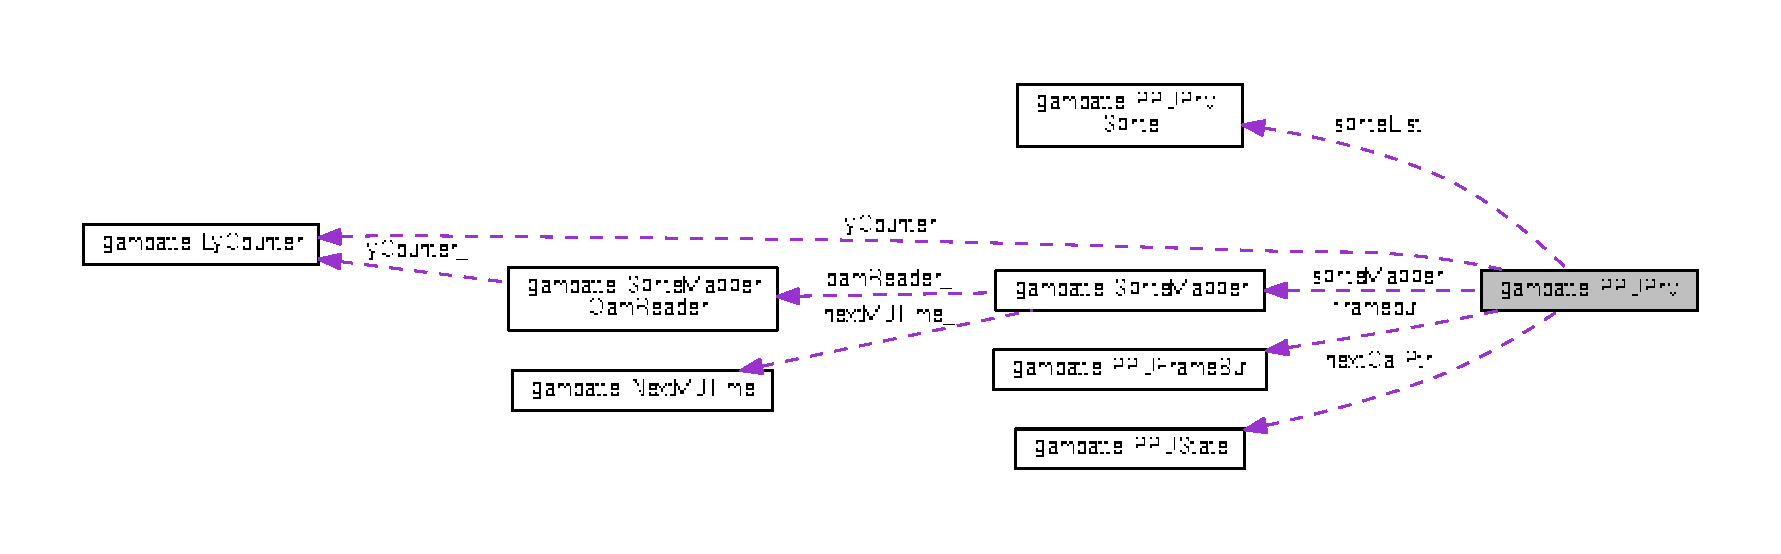
\includegraphics[width=350pt]{structgambatte_1_1PPUPriv__coll__graph}
\end{center}
\end{figure}
\subsection*{Classes}
\begin{DoxyCompactItemize}
\item 
struct \hyperlink{structgambatte_1_1PPUPriv_1_1Sprite}{Sprite}
\end{DoxyCompactItemize}
\subsection*{Public Member Functions}
\begin{DoxyCompactItemize}
\item 
void \hyperlink{structgambatte_1_1PPUPriv_a2d8e18da564e1da4b91c7fac4a11c4a3}{load\+Or\+Save} (\hyperlink{classgambatte_1_1loadsave}{loadsave} \&\hyperlink{ppu_8cpp_a2f2eca6997ee7baf8901725ae074d45b}{state})
\item 
\hyperlink{structgambatte_1_1PPUPriv_a8d7ac334a03adf6ac17861c62f9d1143}{P\+P\+U\+Priv} (\hyperlink{classgambatte_1_1NextM0Time}{Next\+M0\+Time} \&next\+M0\+Time, unsigned char const $\ast$oamram, unsigned char const $\ast$\hyperlink{structgambatte_1_1PPUPriv_a4ab22f440df8bcc60984c9058492dcde}{vram})
\end{DoxyCompactItemize}
\subsection*{Public Attributes}
\begin{DoxyCompactItemize}
\item 
\hyperlink{namespacegambatte_a0639f09fccfbbd5a8e0796318768e370}{uint\+\_\+least32\+\_\+t} \hyperlink{structgambatte_1_1PPUPriv_a9f10e0f050497a5ba47b0fe84bff3450}{bg\+Palette} \mbox{[}8 $\ast$4\mbox{]}
\item 
\hyperlink{namespacegambatte_a0639f09fccfbbd5a8e0796318768e370}{uint\+\_\+least32\+\_\+t} \hyperlink{structgambatte_1_1PPUPriv_a82351915dfa8d9a922bdc335636ee8aa}{sp\+Palette} \mbox{[}8 $\ast$4\mbox{]}
\item 
unsigned char const  $\ast$ \hyperlink{structgambatte_1_1PPUPriv_a4ab22f440df8bcc60984c9058492dcde}{vram}
\item 
\hyperlink{structgambatte_1_1PPUState}{P\+P\+U\+State} const  $\ast$ \hyperlink{structgambatte_1_1PPUPriv_a5e9f54270b9819c6e982585a350b78c2}{next\+Call\+Ptr}
\item 
unsigned \hyperlink{structgambatte_1_1PPUPriv_ab89c0f52942e085ba8168860fd68b006}{now}
\item 
unsigned \hyperlink{structgambatte_1_1PPUPriv_a534222e4b24c8a6479020aaa0fec2e4a}{last\+M0\+Time}
\item 
signed \hyperlink{structgambatte_1_1PPUPriv_a78786db421df1ca669ec10895ad46c47}{cycles}
\item 
unsigned \hyperlink{structgambatte_1_1PPUPriv_a4ab0024dfacb7e9ad1fc89240033a604}{tileword}
\item 
unsigned \hyperlink{structgambatte_1_1PPUPriv_a59f367a6854c749f3c36773e87c47659}{ntileword}
\item 
\hyperlink{classgambatte_1_1LyCounter}{Ly\+Counter} \hyperlink{structgambatte_1_1PPUPriv_aa12c19fee206a403bb5eafea3a696ceb}{ly\+Counter}
\item 
\hyperlink{classgambatte_1_1SpriteMapper}{Sprite\+Mapper} \hyperlink{structgambatte_1_1PPUPriv_af3d873a13e90fb3bf19bca6ee1a35ba5}{sprite\+Mapper}
\item 
\hyperlink{classgambatte_1_1PPUFrameBuf}{P\+P\+U\+Frame\+Buf} \hyperlink{structgambatte_1_1PPUPriv_ab99e1681d0ee5ae3815e6f560de410b2}{framebuf}
\item 
struct \hyperlink{structgambatte_1_1PPUPriv_1_1Sprite}{gambatte\+::\+P\+P\+U\+Priv\+::\+Sprite} \hyperlink{structgambatte_1_1PPUPriv_ac715792e2dbe5fc83c0be7cb444e1726}{sprite\+List} \mbox{[}11\mbox{]}
\item 
unsigned short \hyperlink{structgambatte_1_1PPUPriv_a0f189a633ec3c52b37c9a4be0e96b0cd}{spword\+List} \mbox{[}11\mbox{]}
\item 
unsigned char \hyperlink{structgambatte_1_1PPUPriv_a0e002a001d442d0812736deebd0ba8a1}{lcdc}
\item 
unsigned char \hyperlink{structgambatte_1_1PPUPriv_ac632ba178ee2a53eeb3c98ba13ccc2f5}{scy}
\item 
unsigned char \hyperlink{structgambatte_1_1PPUPriv_af0eae48a849f8cbc06aae956a7e49013}{scx}
\item 
unsigned char \hyperlink{structgambatte_1_1PPUPriv_ace53d0c7b78b568c3ea61b5cd1e39335}{wy}
\item 
unsigned char \hyperlink{structgambatte_1_1PPUPriv_ab2750eac66df777b012b49230730e882}{wy2}
\item 
unsigned char \hyperlink{structgambatte_1_1PPUPriv_a856679c933aab3b5b8846bba59c48e9f}{wx}
\item 
unsigned char \hyperlink{structgambatte_1_1PPUPriv_af25bb3f5b0c93b56d52ac215c8ce2c82}{win\+Draw\+State}
\item 
unsigned char \hyperlink{structgambatte_1_1PPUPriv_a8fdaf8c8c95c7f25392cd2493596946d}{wscx}
\item 
unsigned char \hyperlink{structgambatte_1_1PPUPriv_a1be79e58a77b74d538d5ebdd8d60c6a7}{win\+Y\+Pos}
\item 
unsigned char \hyperlink{structgambatte_1_1PPUPriv_a080d0f22488a104968b72ae88751b7f7}{reg0}
\item 
unsigned char \hyperlink{structgambatte_1_1PPUPriv_a2e589d6d9b5dd0e6f1393eebf263c34a}{reg1}
\item 
unsigned char \hyperlink{structgambatte_1_1PPUPriv_aaf0ca257e082d1eb7ce037e30732893e}{attrib}
\item 
unsigned char \hyperlink{structgambatte_1_1PPUPriv_a62474f22358b00e753c223f75e7d508f}{nattrib}
\item 
unsigned char \hyperlink{structgambatte_1_1PPUPriv_a113d8a8946f77a82a8953a3a4abdf8ca}{next\+Sprite}
\item 
unsigned char \hyperlink{structgambatte_1_1PPUPriv_a0819fddb4da717d7d7ae47262805c696}{current\+Sprite}
\item 
unsigned char \hyperlink{structgambatte_1_1PPUPriv_affeb43eafa62f83c593b3cb14d6241c7}{xpos}
\item 
unsigned char \hyperlink{structgambatte_1_1PPUPriv_a0cbb04bac94de5bc8263a950f4c69033}{endx}
\item 
bool \hyperlink{structgambatte_1_1PPUPriv_a174cd412c81a0bbfe392d34a181e201d}{cgb}
\item 
bool \hyperlink{structgambatte_1_1PPUPriv_ac8b946a2ce5fe6c67159b30d5bae282e}{we\+Master}
\end{DoxyCompactItemize}


\subsection{Constructor \& Destructor Documentation}
\mbox{\Hypertarget{structgambatte_1_1PPUPriv_a8d7ac334a03adf6ac17861c62f9d1143}\label{structgambatte_1_1PPUPriv_a8d7ac334a03adf6ac17861c62f9d1143}} 
\index{gambatte\+::\+P\+P\+U\+Priv@{gambatte\+::\+P\+P\+U\+Priv}!P\+P\+U\+Priv@{P\+P\+U\+Priv}}
\index{P\+P\+U\+Priv@{P\+P\+U\+Priv}!gambatte\+::\+P\+P\+U\+Priv@{gambatte\+::\+P\+P\+U\+Priv}}
\subsubsection{\texorpdfstring{P\+P\+U\+Priv()}{PPUPriv()}}
{\footnotesize\ttfamily gambatte\+::\+P\+P\+U\+Priv\+::\+P\+P\+U\+Priv (\begin{DoxyParamCaption}\item[{\hyperlink{classgambatte_1_1NextM0Time}{Next\+M0\+Time} \&}]{next\+M0\+Time,  }\item[{unsigned char const $\ast$}]{oamram,  }\item[{unsigned char const $\ast$}]{vram }\end{DoxyParamCaption})}



\subsection{Member Function Documentation}
\mbox{\Hypertarget{structgambatte_1_1PPUPriv_a2d8e18da564e1da4b91c7fac4a11c4a3}\label{structgambatte_1_1PPUPriv_a2d8e18da564e1da4b91c7fac4a11c4a3}} 
\index{gambatte\+::\+P\+P\+U\+Priv@{gambatte\+::\+P\+P\+U\+Priv}!load\+Or\+Save@{load\+Or\+Save}}
\index{load\+Or\+Save@{load\+Or\+Save}!gambatte\+::\+P\+P\+U\+Priv@{gambatte\+::\+P\+P\+U\+Priv}}
\subsubsection{\texorpdfstring{load\+Or\+Save()}{loadOrSave()}}
{\footnotesize\ttfamily void gambatte\+::\+P\+P\+U\+Priv\+::load\+Or\+Save (\begin{DoxyParamCaption}\item[{\hyperlink{classgambatte_1_1loadsave}{loadsave} \&}]{state }\end{DoxyParamCaption})}



\subsection{Member Data Documentation}
\mbox{\Hypertarget{structgambatte_1_1PPUPriv_aaf0ca257e082d1eb7ce037e30732893e}\label{structgambatte_1_1PPUPriv_aaf0ca257e082d1eb7ce037e30732893e}} 
\index{gambatte\+::\+P\+P\+U\+Priv@{gambatte\+::\+P\+P\+U\+Priv}!attrib@{attrib}}
\index{attrib@{attrib}!gambatte\+::\+P\+P\+U\+Priv@{gambatte\+::\+P\+P\+U\+Priv}}
\subsubsection{\texorpdfstring{attrib}{attrib}}
{\footnotesize\ttfamily unsigned char gambatte\+::\+P\+P\+U\+Priv\+::attrib}

\mbox{\Hypertarget{structgambatte_1_1PPUPriv_a9f10e0f050497a5ba47b0fe84bff3450}\label{structgambatte_1_1PPUPriv_a9f10e0f050497a5ba47b0fe84bff3450}} 
\index{gambatte\+::\+P\+P\+U\+Priv@{gambatte\+::\+P\+P\+U\+Priv}!bg\+Palette@{bg\+Palette}}
\index{bg\+Palette@{bg\+Palette}!gambatte\+::\+P\+P\+U\+Priv@{gambatte\+::\+P\+P\+U\+Priv}}
\subsubsection{\texorpdfstring{bg\+Palette}{bgPalette}}
{\footnotesize\ttfamily \hyperlink{namespacegambatte_a0639f09fccfbbd5a8e0796318768e370}{uint\+\_\+least32\+\_\+t} gambatte\+::\+P\+P\+U\+Priv\+::bg\+Palette\mbox{[}8 $\ast$4\mbox{]}}

\mbox{\Hypertarget{structgambatte_1_1PPUPriv_a174cd412c81a0bbfe392d34a181e201d}\label{structgambatte_1_1PPUPriv_a174cd412c81a0bbfe392d34a181e201d}} 
\index{gambatte\+::\+P\+P\+U\+Priv@{gambatte\+::\+P\+P\+U\+Priv}!cgb@{cgb}}
\index{cgb@{cgb}!gambatte\+::\+P\+P\+U\+Priv@{gambatte\+::\+P\+P\+U\+Priv}}
\subsubsection{\texorpdfstring{cgb}{cgb}}
{\footnotesize\ttfamily bool gambatte\+::\+P\+P\+U\+Priv\+::cgb}

\mbox{\Hypertarget{structgambatte_1_1PPUPriv_a0819fddb4da717d7d7ae47262805c696}\label{structgambatte_1_1PPUPriv_a0819fddb4da717d7d7ae47262805c696}} 
\index{gambatte\+::\+P\+P\+U\+Priv@{gambatte\+::\+P\+P\+U\+Priv}!current\+Sprite@{current\+Sprite}}
\index{current\+Sprite@{current\+Sprite}!gambatte\+::\+P\+P\+U\+Priv@{gambatte\+::\+P\+P\+U\+Priv}}
\subsubsection{\texorpdfstring{current\+Sprite}{currentSprite}}
{\footnotesize\ttfamily unsigned char gambatte\+::\+P\+P\+U\+Priv\+::current\+Sprite}

\mbox{\Hypertarget{structgambatte_1_1PPUPriv_a78786db421df1ca669ec10895ad46c47}\label{structgambatte_1_1PPUPriv_a78786db421df1ca669ec10895ad46c47}} 
\index{gambatte\+::\+P\+P\+U\+Priv@{gambatte\+::\+P\+P\+U\+Priv}!cycles@{cycles}}
\index{cycles@{cycles}!gambatte\+::\+P\+P\+U\+Priv@{gambatte\+::\+P\+P\+U\+Priv}}
\subsubsection{\texorpdfstring{cycles}{cycles}}
{\footnotesize\ttfamily signed gambatte\+::\+P\+P\+U\+Priv\+::cycles}

\mbox{\Hypertarget{structgambatte_1_1PPUPriv_a0cbb04bac94de5bc8263a950f4c69033}\label{structgambatte_1_1PPUPriv_a0cbb04bac94de5bc8263a950f4c69033}} 
\index{gambatte\+::\+P\+P\+U\+Priv@{gambatte\+::\+P\+P\+U\+Priv}!endx@{endx}}
\index{endx@{endx}!gambatte\+::\+P\+P\+U\+Priv@{gambatte\+::\+P\+P\+U\+Priv}}
\subsubsection{\texorpdfstring{endx}{endx}}
{\footnotesize\ttfamily unsigned char gambatte\+::\+P\+P\+U\+Priv\+::endx}

\mbox{\Hypertarget{structgambatte_1_1PPUPriv_ab99e1681d0ee5ae3815e6f560de410b2}\label{structgambatte_1_1PPUPriv_ab99e1681d0ee5ae3815e6f560de410b2}} 
\index{gambatte\+::\+P\+P\+U\+Priv@{gambatte\+::\+P\+P\+U\+Priv}!framebuf@{framebuf}}
\index{framebuf@{framebuf}!gambatte\+::\+P\+P\+U\+Priv@{gambatte\+::\+P\+P\+U\+Priv}}
\subsubsection{\texorpdfstring{framebuf}{framebuf}}
{\footnotesize\ttfamily \hyperlink{classgambatte_1_1PPUFrameBuf}{P\+P\+U\+Frame\+Buf} gambatte\+::\+P\+P\+U\+Priv\+::framebuf}

\mbox{\Hypertarget{structgambatte_1_1PPUPriv_a534222e4b24c8a6479020aaa0fec2e4a}\label{structgambatte_1_1PPUPriv_a534222e4b24c8a6479020aaa0fec2e4a}} 
\index{gambatte\+::\+P\+P\+U\+Priv@{gambatte\+::\+P\+P\+U\+Priv}!last\+M0\+Time@{last\+M0\+Time}}
\index{last\+M0\+Time@{last\+M0\+Time}!gambatte\+::\+P\+P\+U\+Priv@{gambatte\+::\+P\+P\+U\+Priv}}
\subsubsection{\texorpdfstring{last\+M0\+Time}{lastM0Time}}
{\footnotesize\ttfamily unsigned gambatte\+::\+P\+P\+U\+Priv\+::last\+M0\+Time}

\mbox{\Hypertarget{structgambatte_1_1PPUPriv_a0e002a001d442d0812736deebd0ba8a1}\label{structgambatte_1_1PPUPriv_a0e002a001d442d0812736deebd0ba8a1}} 
\index{gambatte\+::\+P\+P\+U\+Priv@{gambatte\+::\+P\+P\+U\+Priv}!lcdc@{lcdc}}
\index{lcdc@{lcdc}!gambatte\+::\+P\+P\+U\+Priv@{gambatte\+::\+P\+P\+U\+Priv}}
\subsubsection{\texorpdfstring{lcdc}{lcdc}}
{\footnotesize\ttfamily unsigned char gambatte\+::\+P\+P\+U\+Priv\+::lcdc}

\mbox{\Hypertarget{structgambatte_1_1PPUPriv_aa12c19fee206a403bb5eafea3a696ceb}\label{structgambatte_1_1PPUPriv_aa12c19fee206a403bb5eafea3a696ceb}} 
\index{gambatte\+::\+P\+P\+U\+Priv@{gambatte\+::\+P\+P\+U\+Priv}!ly\+Counter@{ly\+Counter}}
\index{ly\+Counter@{ly\+Counter}!gambatte\+::\+P\+P\+U\+Priv@{gambatte\+::\+P\+P\+U\+Priv}}
\subsubsection{\texorpdfstring{ly\+Counter}{lyCounter}}
{\footnotesize\ttfamily \hyperlink{classgambatte_1_1LyCounter}{Ly\+Counter} gambatte\+::\+P\+P\+U\+Priv\+::ly\+Counter}

\mbox{\Hypertarget{structgambatte_1_1PPUPriv_a62474f22358b00e753c223f75e7d508f}\label{structgambatte_1_1PPUPriv_a62474f22358b00e753c223f75e7d508f}} 
\index{gambatte\+::\+P\+P\+U\+Priv@{gambatte\+::\+P\+P\+U\+Priv}!nattrib@{nattrib}}
\index{nattrib@{nattrib}!gambatte\+::\+P\+P\+U\+Priv@{gambatte\+::\+P\+P\+U\+Priv}}
\subsubsection{\texorpdfstring{nattrib}{nattrib}}
{\footnotesize\ttfamily unsigned char gambatte\+::\+P\+P\+U\+Priv\+::nattrib}

\mbox{\Hypertarget{structgambatte_1_1PPUPriv_a5e9f54270b9819c6e982585a350b78c2}\label{structgambatte_1_1PPUPriv_a5e9f54270b9819c6e982585a350b78c2}} 
\index{gambatte\+::\+P\+P\+U\+Priv@{gambatte\+::\+P\+P\+U\+Priv}!next\+Call\+Ptr@{next\+Call\+Ptr}}
\index{next\+Call\+Ptr@{next\+Call\+Ptr}!gambatte\+::\+P\+P\+U\+Priv@{gambatte\+::\+P\+P\+U\+Priv}}
\subsubsection{\texorpdfstring{next\+Call\+Ptr}{nextCallPtr}}
{\footnotesize\ttfamily \hyperlink{structgambatte_1_1PPUState}{P\+P\+U\+State} const$\ast$ gambatte\+::\+P\+P\+U\+Priv\+::next\+Call\+Ptr}

\mbox{\Hypertarget{structgambatte_1_1PPUPriv_a113d8a8946f77a82a8953a3a4abdf8ca}\label{structgambatte_1_1PPUPriv_a113d8a8946f77a82a8953a3a4abdf8ca}} 
\index{gambatte\+::\+P\+P\+U\+Priv@{gambatte\+::\+P\+P\+U\+Priv}!next\+Sprite@{next\+Sprite}}
\index{next\+Sprite@{next\+Sprite}!gambatte\+::\+P\+P\+U\+Priv@{gambatte\+::\+P\+P\+U\+Priv}}
\subsubsection{\texorpdfstring{next\+Sprite}{nextSprite}}
{\footnotesize\ttfamily unsigned char gambatte\+::\+P\+P\+U\+Priv\+::next\+Sprite}

\mbox{\Hypertarget{structgambatte_1_1PPUPriv_ab89c0f52942e085ba8168860fd68b006}\label{structgambatte_1_1PPUPriv_ab89c0f52942e085ba8168860fd68b006}} 
\index{gambatte\+::\+P\+P\+U\+Priv@{gambatte\+::\+P\+P\+U\+Priv}!now@{now}}
\index{now@{now}!gambatte\+::\+P\+P\+U\+Priv@{gambatte\+::\+P\+P\+U\+Priv}}
\subsubsection{\texorpdfstring{now}{now}}
{\footnotesize\ttfamily unsigned gambatte\+::\+P\+P\+U\+Priv\+::now}

\mbox{\Hypertarget{structgambatte_1_1PPUPriv_a59f367a6854c749f3c36773e87c47659}\label{structgambatte_1_1PPUPriv_a59f367a6854c749f3c36773e87c47659}} 
\index{gambatte\+::\+P\+P\+U\+Priv@{gambatte\+::\+P\+P\+U\+Priv}!ntileword@{ntileword}}
\index{ntileword@{ntileword}!gambatte\+::\+P\+P\+U\+Priv@{gambatte\+::\+P\+P\+U\+Priv}}
\subsubsection{\texorpdfstring{ntileword}{ntileword}}
{\footnotesize\ttfamily unsigned gambatte\+::\+P\+P\+U\+Priv\+::ntileword}

\mbox{\Hypertarget{structgambatte_1_1PPUPriv_a080d0f22488a104968b72ae88751b7f7}\label{structgambatte_1_1PPUPriv_a080d0f22488a104968b72ae88751b7f7}} 
\index{gambatte\+::\+P\+P\+U\+Priv@{gambatte\+::\+P\+P\+U\+Priv}!reg0@{reg0}}
\index{reg0@{reg0}!gambatte\+::\+P\+P\+U\+Priv@{gambatte\+::\+P\+P\+U\+Priv}}
\subsubsection{\texorpdfstring{reg0}{reg0}}
{\footnotesize\ttfamily unsigned char gambatte\+::\+P\+P\+U\+Priv\+::reg0}

\mbox{\Hypertarget{structgambatte_1_1PPUPriv_a2e589d6d9b5dd0e6f1393eebf263c34a}\label{structgambatte_1_1PPUPriv_a2e589d6d9b5dd0e6f1393eebf263c34a}} 
\index{gambatte\+::\+P\+P\+U\+Priv@{gambatte\+::\+P\+P\+U\+Priv}!reg1@{reg1}}
\index{reg1@{reg1}!gambatte\+::\+P\+P\+U\+Priv@{gambatte\+::\+P\+P\+U\+Priv}}
\subsubsection{\texorpdfstring{reg1}{reg1}}
{\footnotesize\ttfamily unsigned char gambatte\+::\+P\+P\+U\+Priv\+::reg1}

\mbox{\Hypertarget{structgambatte_1_1PPUPriv_af0eae48a849f8cbc06aae956a7e49013}\label{structgambatte_1_1PPUPriv_af0eae48a849f8cbc06aae956a7e49013}} 
\index{gambatte\+::\+P\+P\+U\+Priv@{gambatte\+::\+P\+P\+U\+Priv}!scx@{scx}}
\index{scx@{scx}!gambatte\+::\+P\+P\+U\+Priv@{gambatte\+::\+P\+P\+U\+Priv}}
\subsubsection{\texorpdfstring{scx}{scx}}
{\footnotesize\ttfamily unsigned char gambatte\+::\+P\+P\+U\+Priv\+::scx}

\mbox{\Hypertarget{structgambatte_1_1PPUPriv_ac632ba178ee2a53eeb3c98ba13ccc2f5}\label{structgambatte_1_1PPUPriv_ac632ba178ee2a53eeb3c98ba13ccc2f5}} 
\index{gambatte\+::\+P\+P\+U\+Priv@{gambatte\+::\+P\+P\+U\+Priv}!scy@{scy}}
\index{scy@{scy}!gambatte\+::\+P\+P\+U\+Priv@{gambatte\+::\+P\+P\+U\+Priv}}
\subsubsection{\texorpdfstring{scy}{scy}}
{\footnotesize\ttfamily unsigned char gambatte\+::\+P\+P\+U\+Priv\+::scy}

\mbox{\Hypertarget{structgambatte_1_1PPUPriv_a82351915dfa8d9a922bdc335636ee8aa}\label{structgambatte_1_1PPUPriv_a82351915dfa8d9a922bdc335636ee8aa}} 
\index{gambatte\+::\+P\+P\+U\+Priv@{gambatte\+::\+P\+P\+U\+Priv}!sp\+Palette@{sp\+Palette}}
\index{sp\+Palette@{sp\+Palette}!gambatte\+::\+P\+P\+U\+Priv@{gambatte\+::\+P\+P\+U\+Priv}}
\subsubsection{\texorpdfstring{sp\+Palette}{spPalette}}
{\footnotesize\ttfamily \hyperlink{namespacegambatte_a0639f09fccfbbd5a8e0796318768e370}{uint\+\_\+least32\+\_\+t} gambatte\+::\+P\+P\+U\+Priv\+::sp\+Palette\mbox{[}8 $\ast$4\mbox{]}}

\mbox{\Hypertarget{structgambatte_1_1PPUPriv_ac715792e2dbe5fc83c0be7cb444e1726}\label{structgambatte_1_1PPUPriv_ac715792e2dbe5fc83c0be7cb444e1726}} 
\index{gambatte\+::\+P\+P\+U\+Priv@{gambatte\+::\+P\+P\+U\+Priv}!sprite\+List@{sprite\+List}}
\index{sprite\+List@{sprite\+List}!gambatte\+::\+P\+P\+U\+Priv@{gambatte\+::\+P\+P\+U\+Priv}}
\subsubsection{\texorpdfstring{sprite\+List}{spriteList}}
{\footnotesize\ttfamily struct \hyperlink{structgambatte_1_1PPUPriv_1_1Sprite}{gambatte\+::\+P\+P\+U\+Priv\+::\+Sprite}  gambatte\+::\+P\+P\+U\+Priv\+::sprite\+List\mbox{[}11\mbox{]}}

\mbox{\Hypertarget{structgambatte_1_1PPUPriv_af3d873a13e90fb3bf19bca6ee1a35ba5}\label{structgambatte_1_1PPUPriv_af3d873a13e90fb3bf19bca6ee1a35ba5}} 
\index{gambatte\+::\+P\+P\+U\+Priv@{gambatte\+::\+P\+P\+U\+Priv}!sprite\+Mapper@{sprite\+Mapper}}
\index{sprite\+Mapper@{sprite\+Mapper}!gambatte\+::\+P\+P\+U\+Priv@{gambatte\+::\+P\+P\+U\+Priv}}
\subsubsection{\texorpdfstring{sprite\+Mapper}{spriteMapper}}
{\footnotesize\ttfamily \hyperlink{classgambatte_1_1SpriteMapper}{Sprite\+Mapper} gambatte\+::\+P\+P\+U\+Priv\+::sprite\+Mapper}

\mbox{\Hypertarget{structgambatte_1_1PPUPriv_a0f189a633ec3c52b37c9a4be0e96b0cd}\label{structgambatte_1_1PPUPriv_a0f189a633ec3c52b37c9a4be0e96b0cd}} 
\index{gambatte\+::\+P\+P\+U\+Priv@{gambatte\+::\+P\+P\+U\+Priv}!spword\+List@{spword\+List}}
\index{spword\+List@{spword\+List}!gambatte\+::\+P\+P\+U\+Priv@{gambatte\+::\+P\+P\+U\+Priv}}
\subsubsection{\texorpdfstring{spword\+List}{spwordList}}
{\footnotesize\ttfamily unsigned short gambatte\+::\+P\+P\+U\+Priv\+::spword\+List\mbox{[}11\mbox{]}}

\mbox{\Hypertarget{structgambatte_1_1PPUPriv_a4ab0024dfacb7e9ad1fc89240033a604}\label{structgambatte_1_1PPUPriv_a4ab0024dfacb7e9ad1fc89240033a604}} 
\index{gambatte\+::\+P\+P\+U\+Priv@{gambatte\+::\+P\+P\+U\+Priv}!tileword@{tileword}}
\index{tileword@{tileword}!gambatte\+::\+P\+P\+U\+Priv@{gambatte\+::\+P\+P\+U\+Priv}}
\subsubsection{\texorpdfstring{tileword}{tileword}}
{\footnotesize\ttfamily unsigned gambatte\+::\+P\+P\+U\+Priv\+::tileword}

\mbox{\Hypertarget{structgambatte_1_1PPUPriv_a4ab22f440df8bcc60984c9058492dcde}\label{structgambatte_1_1PPUPriv_a4ab22f440df8bcc60984c9058492dcde}} 
\index{gambatte\+::\+P\+P\+U\+Priv@{gambatte\+::\+P\+P\+U\+Priv}!vram@{vram}}
\index{vram@{vram}!gambatte\+::\+P\+P\+U\+Priv@{gambatte\+::\+P\+P\+U\+Priv}}
\subsubsection{\texorpdfstring{vram}{vram}}
{\footnotesize\ttfamily unsigned char const$\ast$ gambatte\+::\+P\+P\+U\+Priv\+::vram}

\mbox{\Hypertarget{structgambatte_1_1PPUPriv_ac8b946a2ce5fe6c67159b30d5bae282e}\label{structgambatte_1_1PPUPriv_ac8b946a2ce5fe6c67159b30d5bae282e}} 
\index{gambatte\+::\+P\+P\+U\+Priv@{gambatte\+::\+P\+P\+U\+Priv}!we\+Master@{we\+Master}}
\index{we\+Master@{we\+Master}!gambatte\+::\+P\+P\+U\+Priv@{gambatte\+::\+P\+P\+U\+Priv}}
\subsubsection{\texorpdfstring{we\+Master}{weMaster}}
{\footnotesize\ttfamily bool gambatte\+::\+P\+P\+U\+Priv\+::we\+Master}

\mbox{\Hypertarget{structgambatte_1_1PPUPriv_af25bb3f5b0c93b56d52ac215c8ce2c82}\label{structgambatte_1_1PPUPriv_af25bb3f5b0c93b56d52ac215c8ce2c82}} 
\index{gambatte\+::\+P\+P\+U\+Priv@{gambatte\+::\+P\+P\+U\+Priv}!win\+Draw\+State@{win\+Draw\+State}}
\index{win\+Draw\+State@{win\+Draw\+State}!gambatte\+::\+P\+P\+U\+Priv@{gambatte\+::\+P\+P\+U\+Priv}}
\subsubsection{\texorpdfstring{win\+Draw\+State}{winDrawState}}
{\footnotesize\ttfamily unsigned char gambatte\+::\+P\+P\+U\+Priv\+::win\+Draw\+State}

\mbox{\Hypertarget{structgambatte_1_1PPUPriv_a1be79e58a77b74d538d5ebdd8d60c6a7}\label{structgambatte_1_1PPUPriv_a1be79e58a77b74d538d5ebdd8d60c6a7}} 
\index{gambatte\+::\+P\+P\+U\+Priv@{gambatte\+::\+P\+P\+U\+Priv}!win\+Y\+Pos@{win\+Y\+Pos}}
\index{win\+Y\+Pos@{win\+Y\+Pos}!gambatte\+::\+P\+P\+U\+Priv@{gambatte\+::\+P\+P\+U\+Priv}}
\subsubsection{\texorpdfstring{win\+Y\+Pos}{winYPos}}
{\footnotesize\ttfamily unsigned char gambatte\+::\+P\+P\+U\+Priv\+::win\+Y\+Pos}

\mbox{\Hypertarget{structgambatte_1_1PPUPriv_a8fdaf8c8c95c7f25392cd2493596946d}\label{structgambatte_1_1PPUPriv_a8fdaf8c8c95c7f25392cd2493596946d}} 
\index{gambatte\+::\+P\+P\+U\+Priv@{gambatte\+::\+P\+P\+U\+Priv}!wscx@{wscx}}
\index{wscx@{wscx}!gambatte\+::\+P\+P\+U\+Priv@{gambatte\+::\+P\+P\+U\+Priv}}
\subsubsection{\texorpdfstring{wscx}{wscx}}
{\footnotesize\ttfamily unsigned char gambatte\+::\+P\+P\+U\+Priv\+::wscx}

\mbox{\Hypertarget{structgambatte_1_1PPUPriv_a856679c933aab3b5b8846bba59c48e9f}\label{structgambatte_1_1PPUPriv_a856679c933aab3b5b8846bba59c48e9f}} 
\index{gambatte\+::\+P\+P\+U\+Priv@{gambatte\+::\+P\+P\+U\+Priv}!wx@{wx}}
\index{wx@{wx}!gambatte\+::\+P\+P\+U\+Priv@{gambatte\+::\+P\+P\+U\+Priv}}
\subsubsection{\texorpdfstring{wx}{wx}}
{\footnotesize\ttfamily unsigned char gambatte\+::\+P\+P\+U\+Priv\+::wx}

\mbox{\Hypertarget{structgambatte_1_1PPUPriv_ace53d0c7b78b568c3ea61b5cd1e39335}\label{structgambatte_1_1PPUPriv_ace53d0c7b78b568c3ea61b5cd1e39335}} 
\index{gambatte\+::\+P\+P\+U\+Priv@{gambatte\+::\+P\+P\+U\+Priv}!wy@{wy}}
\index{wy@{wy}!gambatte\+::\+P\+P\+U\+Priv@{gambatte\+::\+P\+P\+U\+Priv}}
\subsubsection{\texorpdfstring{wy}{wy}}
{\footnotesize\ttfamily unsigned char gambatte\+::\+P\+P\+U\+Priv\+::wy}

\mbox{\Hypertarget{structgambatte_1_1PPUPriv_ab2750eac66df777b012b49230730e882}\label{structgambatte_1_1PPUPriv_ab2750eac66df777b012b49230730e882}} 
\index{gambatte\+::\+P\+P\+U\+Priv@{gambatte\+::\+P\+P\+U\+Priv}!wy2@{wy2}}
\index{wy2@{wy2}!gambatte\+::\+P\+P\+U\+Priv@{gambatte\+::\+P\+P\+U\+Priv}}
\subsubsection{\texorpdfstring{wy2}{wy2}}
{\footnotesize\ttfamily unsigned char gambatte\+::\+P\+P\+U\+Priv\+::wy2}

\mbox{\Hypertarget{structgambatte_1_1PPUPriv_affeb43eafa62f83c593b3cb14d6241c7}\label{structgambatte_1_1PPUPriv_affeb43eafa62f83c593b3cb14d6241c7}} 
\index{gambatte\+::\+P\+P\+U\+Priv@{gambatte\+::\+P\+P\+U\+Priv}!xpos@{xpos}}
\index{xpos@{xpos}!gambatte\+::\+P\+P\+U\+Priv@{gambatte\+::\+P\+P\+U\+Priv}}
\subsubsection{\texorpdfstring{xpos}{xpos}}
{\footnotesize\ttfamily unsigned char gambatte\+::\+P\+P\+U\+Priv\+::xpos}



The documentation for this struct was generated from the following files\+:\begin{DoxyCompactItemize}
\item 
src/video/\hyperlink{ppu_8h}{ppu.\+h}\item 
src/video/\hyperlink{ppu_8cpp}{ppu.\+cpp}\end{DoxyCompactItemize}

\hypertarget{structgambatte_1_1PPUState}{}\section{gambatte\+:\+:P\+P\+U\+State Struct Reference}
\label{structgambatte_1_1PPUState}\index{gambatte\+::\+P\+P\+U\+State@{gambatte\+::\+P\+P\+U\+State}}


{\ttfamily \#include $<$ppu.\+h$>$}

\subsection*{Public Attributes}
\begin{DoxyCompactItemize}
\item 
void($\ast$ \hyperlink{structgambatte_1_1PPUState_a995de491176aba32c43617e4f255d57b}{f} )(\hyperlink{structgambatte_1_1PPUPriv}{P\+P\+U\+Priv} \&v)
\item 
unsigned($\ast$ \hyperlink{structgambatte_1_1PPUState_a6eb2480038e1ff8e9e1ee59d1486ade9}{predict\+Cycles\+Until\+Xpos\+\_\+f} )(\hyperlink{structgambatte_1_1PPUPriv}{P\+P\+U\+Priv} const \&v, \hyperlink{ioapi_8h_a787fa3cf048117ba7123753c1e74fcd6}{int} targetxpos, unsigned cycles)
\item 
unsigned char \hyperlink{structgambatte_1_1PPUState_a5365ffcae4c4cec4178cae3c014d561b}{id}
\end{DoxyCompactItemize}


\subsection{Member Data Documentation}
\mbox{\Hypertarget{structgambatte_1_1PPUState_a995de491176aba32c43617e4f255d57b}\label{structgambatte_1_1PPUState_a995de491176aba32c43617e4f255d57b}} 
\index{gambatte\+::\+P\+P\+U\+State@{gambatte\+::\+P\+P\+U\+State}!f@{f}}
\index{f@{f}!gambatte\+::\+P\+P\+U\+State@{gambatte\+::\+P\+P\+U\+State}}
\subsubsection{\texorpdfstring{f}{f}}
{\footnotesize\ttfamily void($\ast$ gambatte\+::\+P\+P\+U\+State\+::f) (\hyperlink{structgambatte_1_1PPUPriv}{P\+P\+U\+Priv} \&v)}

\mbox{\Hypertarget{structgambatte_1_1PPUState_a5365ffcae4c4cec4178cae3c014d561b}\label{structgambatte_1_1PPUState_a5365ffcae4c4cec4178cae3c014d561b}} 
\index{gambatte\+::\+P\+P\+U\+State@{gambatte\+::\+P\+P\+U\+State}!id@{id}}
\index{id@{id}!gambatte\+::\+P\+P\+U\+State@{gambatte\+::\+P\+P\+U\+State}}
\subsubsection{\texorpdfstring{id}{id}}
{\footnotesize\ttfamily unsigned char gambatte\+::\+P\+P\+U\+State\+::id}

\mbox{\Hypertarget{structgambatte_1_1PPUState_a6eb2480038e1ff8e9e1ee59d1486ade9}\label{structgambatte_1_1PPUState_a6eb2480038e1ff8e9e1ee59d1486ade9}} 
\index{gambatte\+::\+P\+P\+U\+State@{gambatte\+::\+P\+P\+U\+State}!predict\+Cycles\+Until\+Xpos\+\_\+f@{predict\+Cycles\+Until\+Xpos\+\_\+f}}
\index{predict\+Cycles\+Until\+Xpos\+\_\+f@{predict\+Cycles\+Until\+Xpos\+\_\+f}!gambatte\+::\+P\+P\+U\+State@{gambatte\+::\+P\+P\+U\+State}}
\subsubsection{\texorpdfstring{predict\+Cycles\+Until\+Xpos\+\_\+f}{predictCyclesUntilXpos\_f}}
{\footnotesize\ttfamily unsigned($\ast$ gambatte\+::\+P\+P\+U\+State\+::predict\+Cycles\+Until\+Xpos\+\_\+f) (\hyperlink{structgambatte_1_1PPUPriv}{P\+P\+U\+Priv} const \&v, \hyperlink{ioapi_8h_a787fa3cf048117ba7123753c1e74fcd6}{int} targetxpos, unsigned cycles)}



The documentation for this struct was generated from the following file\+:\begin{DoxyCompactItemize}
\item 
src/video/\hyperlink{ppu_8h}{ppu.\+h}\end{DoxyCompactItemize}

\hypertarget{structgambatte_1_1GB_1_1Priv}{}\section{gambatte\+:\+:GB\+:\+:Priv Struct Reference}
\label{structgambatte_1_1GB_1_1Priv}\index{gambatte\+::\+G\+B\+::\+Priv@{gambatte\+::\+G\+B\+::\+Priv}}


Collaboration diagram for gambatte\+:\+:GB\+:\+:Priv\+:
\nopagebreak
\begin{figure}[H]
\begin{center}
\leavevmode
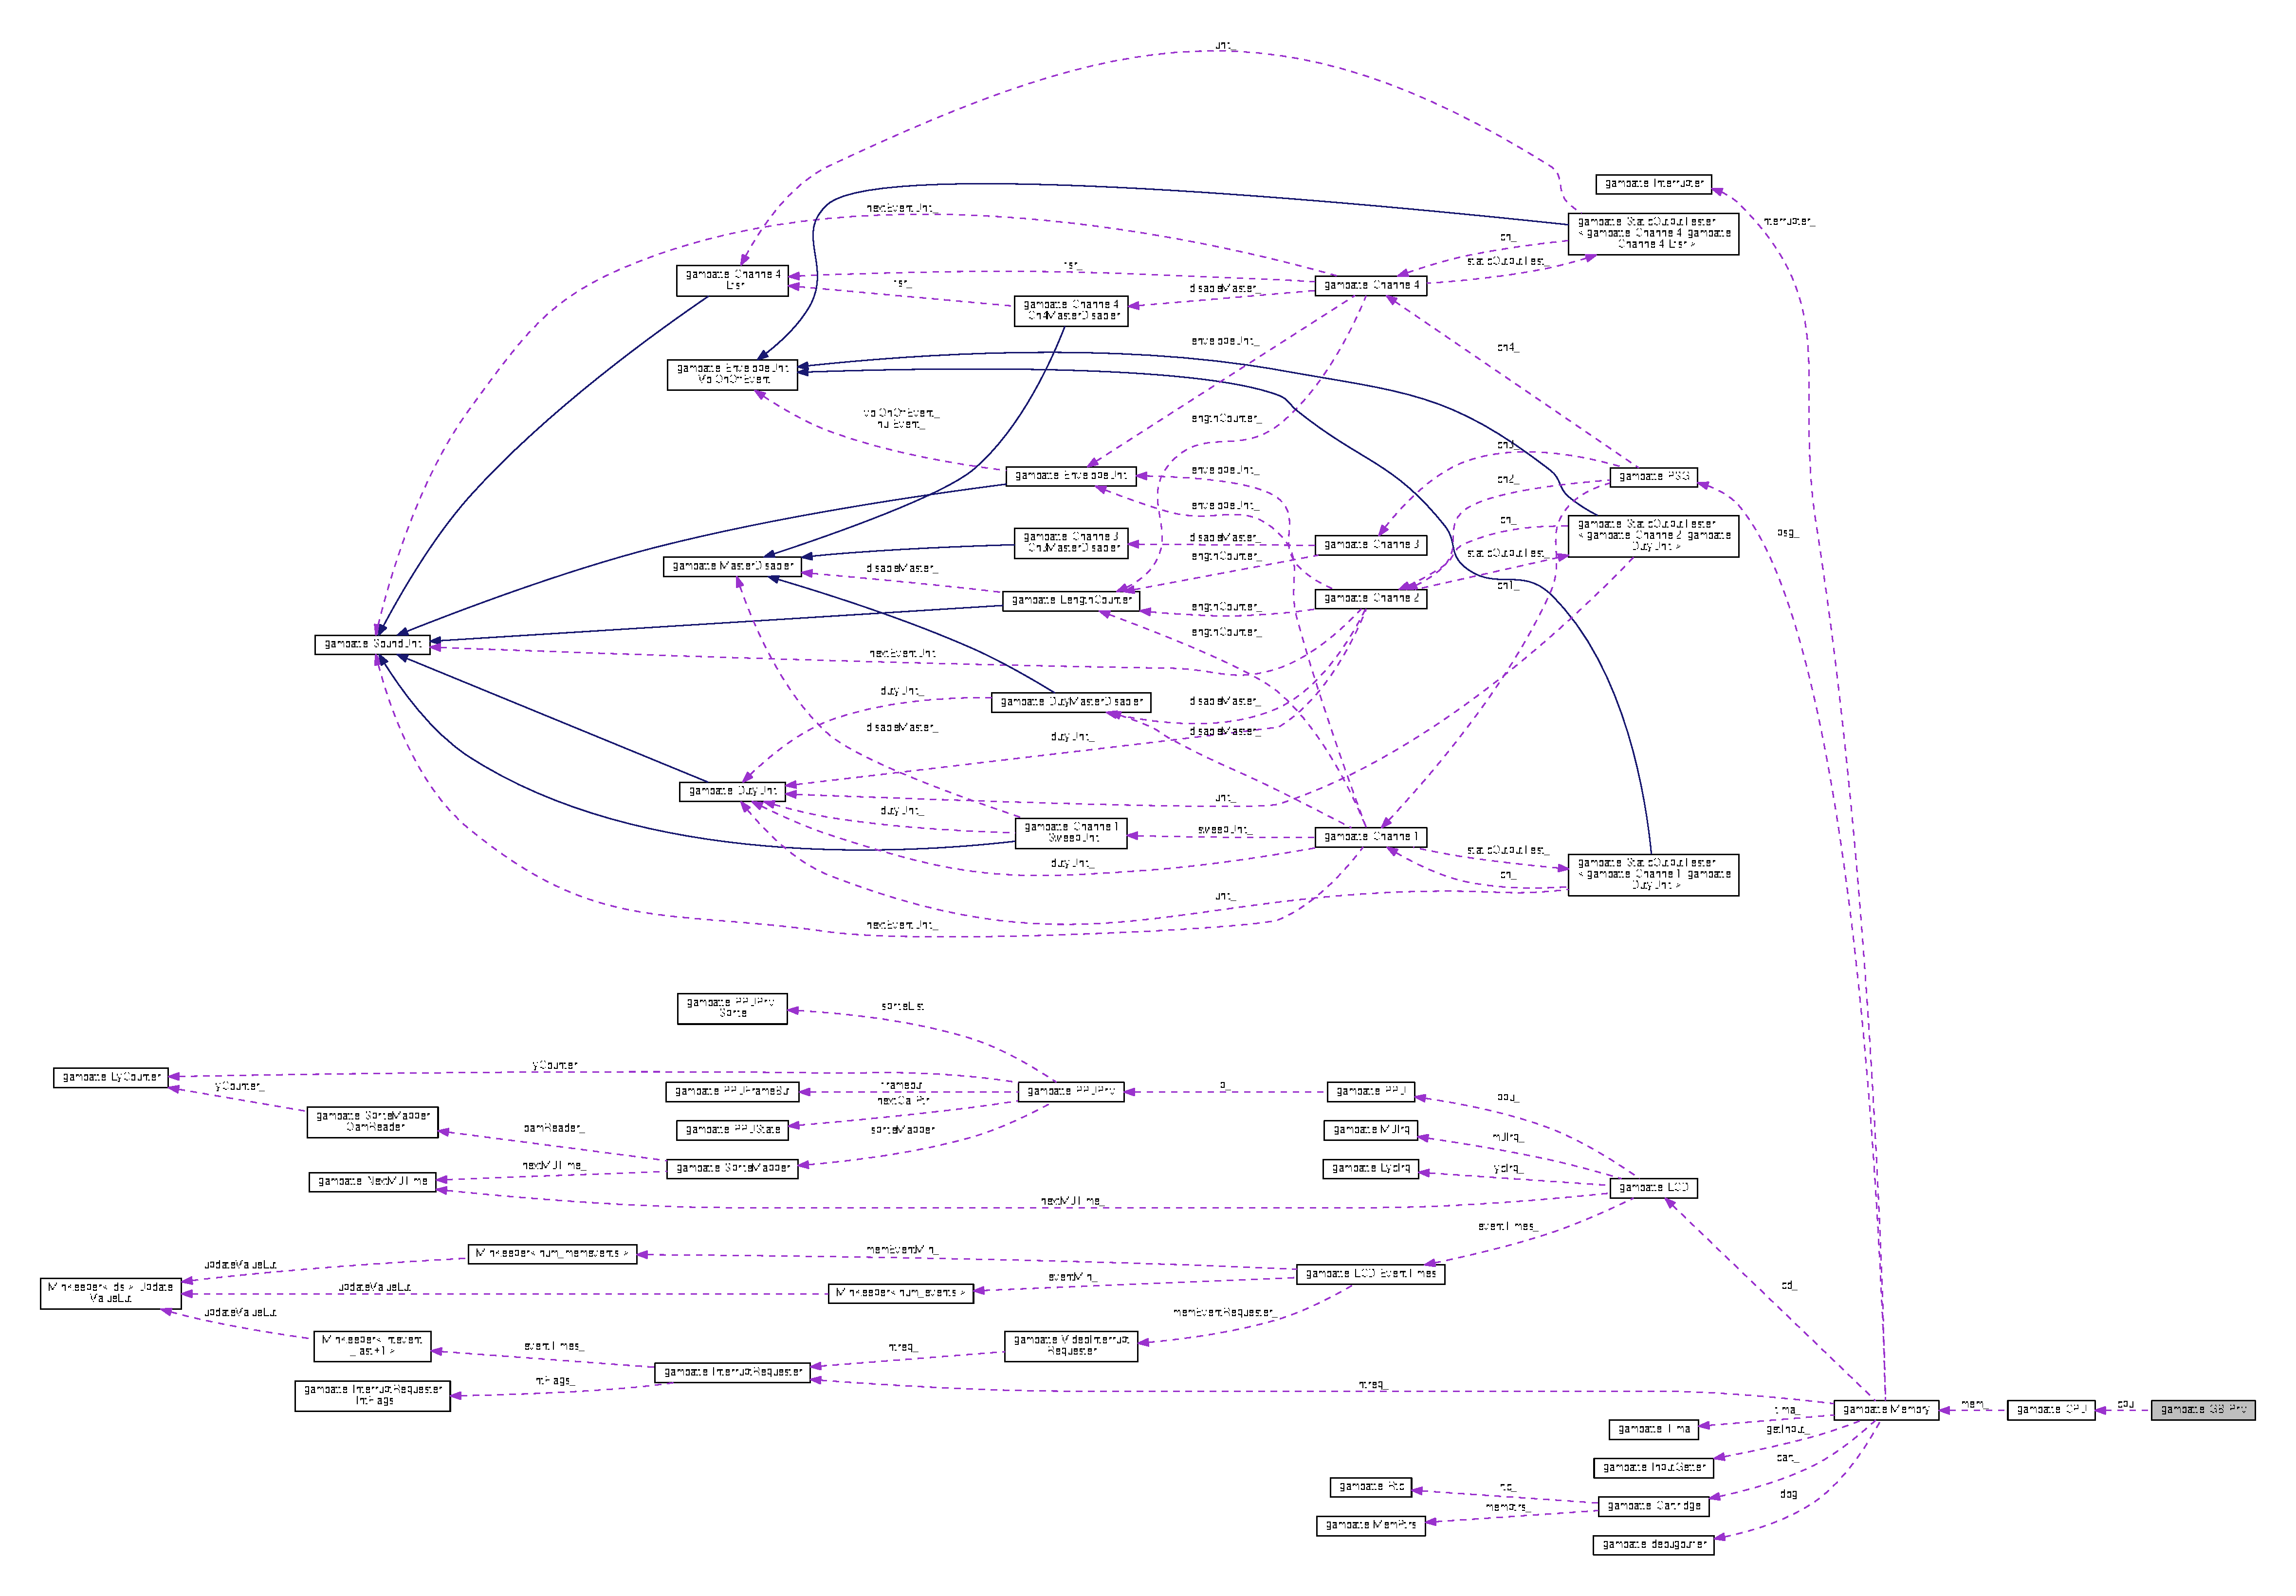
\includegraphics[width=350pt]{structgambatte_1_1GB_1_1Priv__coll__graph}
\end{center}
\end{figure}
\subsection*{Public Member Functions}
\begin{DoxyCompactItemize}
\item 
\hyperlink{structgambatte_1_1GB_1_1Priv_a2d1cc0005de51b6689fae944b124e4a4}{Priv} (time\+\_\+t($\ast$$\ast$\+\_\+get\+Current\+Time)())
\end{DoxyCompactItemize}
\subsection*{Public Attributes}
\begin{DoxyCompactItemize}
\item 
\hyperlink{classgambatte_1_1CPU}{C\+PU} \hyperlink{structgambatte_1_1GB_1_1Priv_addcc3d5369c9e5a82aedcf915112b168}{cpu}
\item 
\hyperlink{ioapi_8h_a787fa3cf048117ba7123753c1e74fcd6}{int} \hyperlink{structgambatte_1_1GB_1_1Priv_ae942db4bbe5234a0ae60abf44be98357}{state\+No}
\item 
unsigned \hyperlink{structgambatte_1_1GB_1_1Priv_a9d8c9106fc5dcceaf418b53cfbd8e357}{loadflags}
\end{DoxyCompactItemize}


\subsection{Constructor \& Destructor Documentation}
\mbox{\Hypertarget{structgambatte_1_1GB_1_1Priv_a2d1cc0005de51b6689fae944b124e4a4}\label{structgambatte_1_1GB_1_1Priv_a2d1cc0005de51b6689fae944b124e4a4}} 
\index{gambatte\+::\+G\+B\+::\+Priv@{gambatte\+::\+G\+B\+::\+Priv}!Priv@{Priv}}
\index{Priv@{Priv}!gambatte\+::\+G\+B\+::\+Priv@{gambatte\+::\+G\+B\+::\+Priv}}
\subsubsection{\texorpdfstring{Priv()}{Priv()}}
{\footnotesize\ttfamily gambatte\+::\+G\+B\+::\+Priv\+::\+Priv (\begin{DoxyParamCaption}\item[{time\+\_\+t($\ast$$\ast$)()}]{\+\_\+get\+Current\+Time }\end{DoxyParamCaption})\hspace{0.3cm}{\ttfamily [inline]}}



\subsection{Member Data Documentation}
\mbox{\Hypertarget{structgambatte_1_1GB_1_1Priv_addcc3d5369c9e5a82aedcf915112b168}\label{structgambatte_1_1GB_1_1Priv_addcc3d5369c9e5a82aedcf915112b168}} 
\index{gambatte\+::\+G\+B\+::\+Priv@{gambatte\+::\+G\+B\+::\+Priv}!cpu@{cpu}}
\index{cpu@{cpu}!gambatte\+::\+G\+B\+::\+Priv@{gambatte\+::\+G\+B\+::\+Priv}}
\subsubsection{\texorpdfstring{cpu}{cpu}}
{\footnotesize\ttfamily \hyperlink{classgambatte_1_1CPU}{C\+PU} gambatte\+::\+G\+B\+::\+Priv\+::cpu}

\mbox{\Hypertarget{structgambatte_1_1GB_1_1Priv_a9d8c9106fc5dcceaf418b53cfbd8e357}\label{structgambatte_1_1GB_1_1Priv_a9d8c9106fc5dcceaf418b53cfbd8e357}} 
\index{gambatte\+::\+G\+B\+::\+Priv@{gambatte\+::\+G\+B\+::\+Priv}!loadflags@{loadflags}}
\index{loadflags@{loadflags}!gambatte\+::\+G\+B\+::\+Priv@{gambatte\+::\+G\+B\+::\+Priv}}
\subsubsection{\texorpdfstring{loadflags}{loadflags}}
{\footnotesize\ttfamily unsigned gambatte\+::\+G\+B\+::\+Priv\+::loadflags}

\mbox{\Hypertarget{structgambatte_1_1GB_1_1Priv_ae942db4bbe5234a0ae60abf44be98357}\label{structgambatte_1_1GB_1_1Priv_ae942db4bbe5234a0ae60abf44be98357}} 
\index{gambatte\+::\+G\+B\+::\+Priv@{gambatte\+::\+G\+B\+::\+Priv}!state\+No@{state\+No}}
\index{state\+No@{state\+No}!gambatte\+::\+G\+B\+::\+Priv@{gambatte\+::\+G\+B\+::\+Priv}}
\subsubsection{\texorpdfstring{state\+No}{stateNo}}
{\footnotesize\ttfamily \hyperlink{ioapi_8h_a787fa3cf048117ba7123753c1e74fcd6}{int} gambatte\+::\+G\+B\+::\+Priv\+::state\+No}



The documentation for this struct was generated from the following file\+:\begin{DoxyCompactItemize}
\item 
src/\hyperlink{gambatte_8cpp}{gambatte.\+cpp}\end{DoxyCompactItemize}

\hypertarget{classgambatte_1_1PSG}{}\section{gambatte\+:\+:P\+SG Class Reference}
\label{classgambatte_1_1PSG}\index{gambatte\+::\+P\+SG@{gambatte\+::\+P\+SG}}


{\ttfamily \#include $<$sound.\+h$>$}



Collaboration diagram for gambatte\+:\+:P\+SG\+:
\nopagebreak
\begin{figure}[H]
\begin{center}
\leavevmode
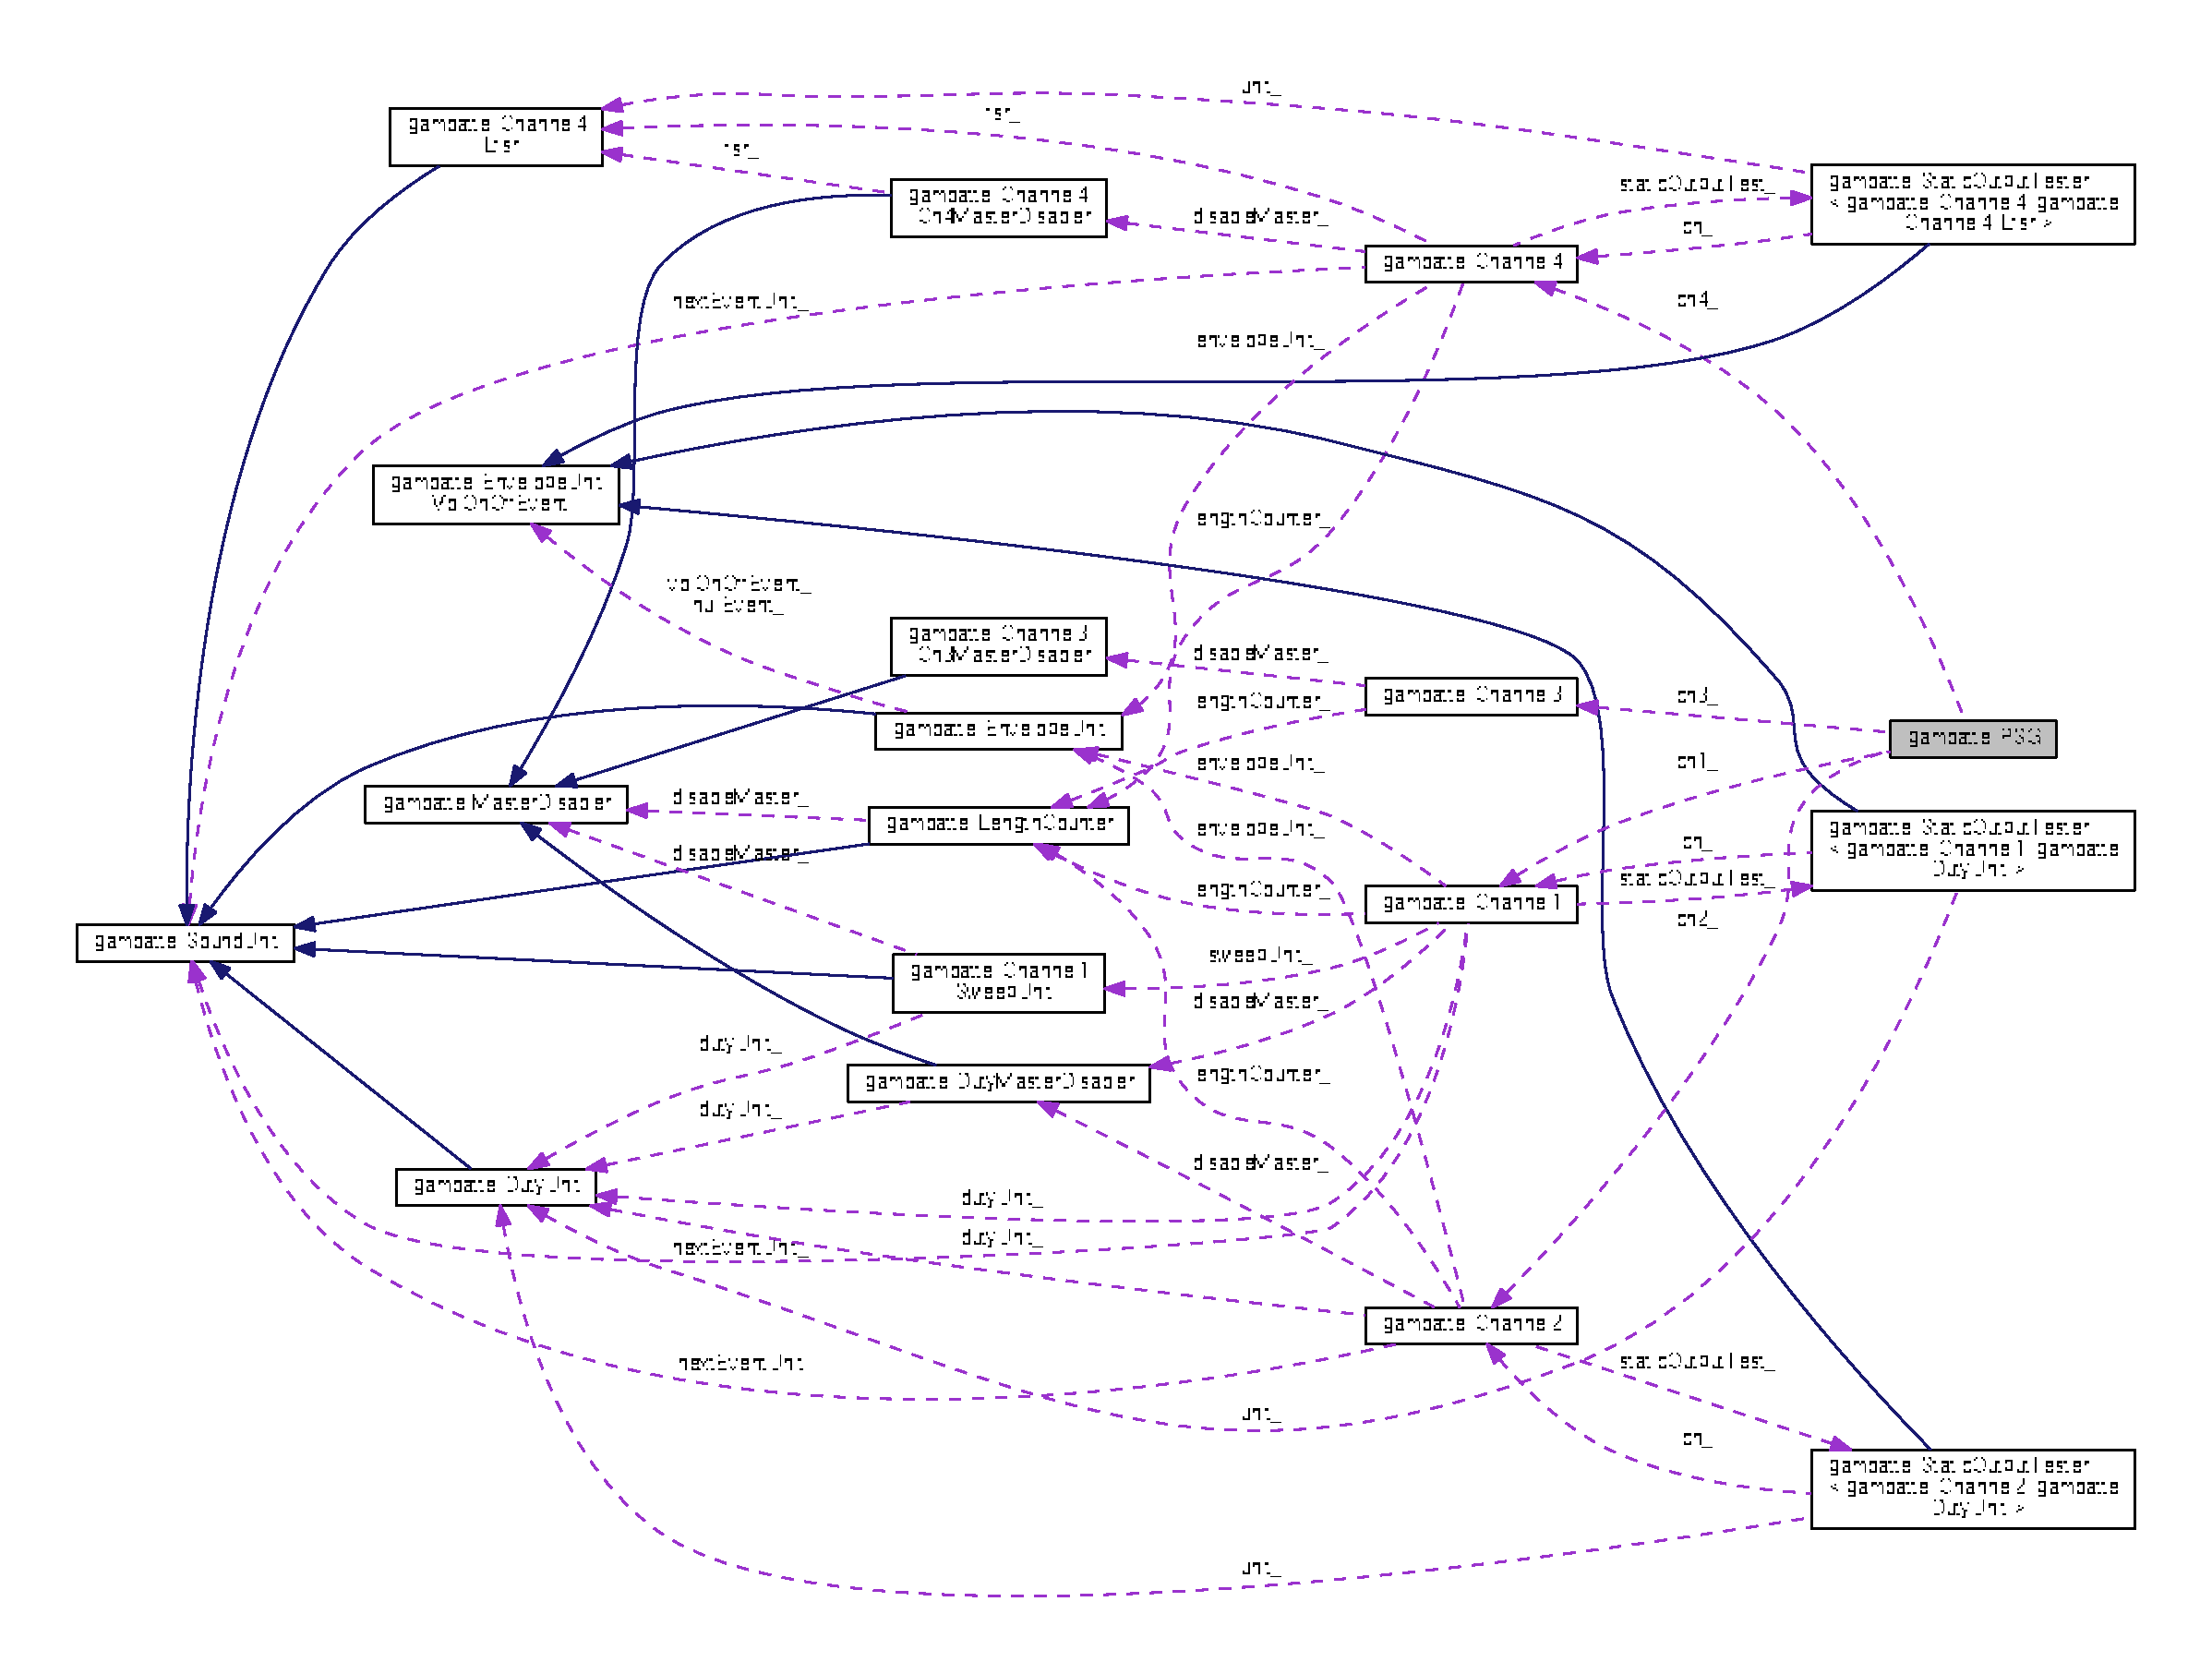
\includegraphics[width=350pt]{classgambatte_1_1PSG__coll__graph}
\end{center}
\end{figure}
\subsection*{Public Member Functions}
\begin{DoxyCompactItemize}
\item 
\hyperlink{classgambatte_1_1PSG_aa3dd35671196e7caf03ab488fa6768ed}{P\+SG} ()
\item 
void \hyperlink{classgambatte_1_1PSG_a8c1f386bd9da8395aeb66dee7059b7fe}{init} (bool cgb)
\item 
void \hyperlink{classgambatte_1_1PSG_af899b7b1de13a7abb0f1aa3e33be7dd1}{reset} ()
\item 
void \hyperlink{classgambatte_1_1PSG_ae232a6e30755b72d1af0d11e03729dc3}{set\+State\+Ptrs} (\hyperlink{structgambatte_1_1SaveState}{Save\+State} \&\hyperlink{ppu_8cpp_a2f2eca6997ee7baf8901725ae074d45b}{state})
\item 
void \hyperlink{classgambatte_1_1PSG_a2b892219d0ea5bf3f7954e2e68e3f7f6}{save\+State} (\hyperlink{structgambatte_1_1SaveState}{Save\+State} \&\hyperlink{ppu_8cpp_a2f2eca6997ee7baf8901725ae074d45b}{state})
\item 
void \hyperlink{classgambatte_1_1PSG_a302cc5f1d4500deaee2ba342e6470b47}{load\+State} (\hyperlink{structgambatte_1_1SaveState}{Save\+State} const \&\hyperlink{ppu_8cpp_a2f2eca6997ee7baf8901725ae074d45b}{state})
\item 
void \hyperlink{classgambatte_1_1PSG_aa40355bad44e2ba8981d42160b92e622}{load\+Or\+Save} (\hyperlink{classgambatte_1_1loadsave}{loadsave} \&\hyperlink{ppu_8cpp_a2f2eca6997ee7baf8901725ae074d45b}{state})
\item 
void \hyperlink{classgambatte_1_1PSG_a9bcdc6e6a7ba05527a6d09b2cb0ceaca}{generate\+Samples} (unsigned cycle\+Counter, bool double\+Speed)
\item 
void \hyperlink{classgambatte_1_1PSG_ab3ad75652ca8508592a7a55df874d4ca}{reset\+Counter} (unsigned new\+Cc, unsigned old\+Cc, bool double\+Speed)
\item 
unsigned \hyperlink{classgambatte_1_1PSG_a81ef34b06def903ab8a24ab485d07b95}{fill\+Buffer} ()
\item 
void \hyperlink{classgambatte_1_1PSG_a7c5a2474671eac749dc35959f76762d3}{set\+Buffer} (\hyperlink{namespacegambatte_a0639f09fccfbbd5a8e0796318768e370}{uint\+\_\+least32\+\_\+t} $\ast$\hyperlink{ioapi_8h_a8ad8a13c88886b9f623034ff88570adb}{buf})
\item 
bool \hyperlink{classgambatte_1_1PSG_ac066ac94f030d1fe6bcc56d8fdfc34b2}{is\+Enabled} () const
\item 
void \hyperlink{classgambatte_1_1PSG_a4186a8804aef89c37b5c7bd0e226d911}{set\+Enabled} (bool value)
\item 
void \hyperlink{classgambatte_1_1PSG_a81254f4d126220d73fbba4e49faa001e}{set\+Nr10} (unsigned data)
\item 
void \hyperlink{classgambatte_1_1PSG_a808c7eeb314688f6bfcf99769cff4750}{set\+Nr11} (unsigned data)
\item 
void \hyperlink{classgambatte_1_1PSG_ac8ee32dcc76c89ed380fd54ea1221b93}{set\+Nr12} (unsigned data)
\item 
void \hyperlink{classgambatte_1_1PSG_a7efd38111196e78e40c5f67460a93ad5}{set\+Nr13} (unsigned data)
\item 
void \hyperlink{classgambatte_1_1PSG_a86567a2fb104433f3c05643bba9072df}{set\+Nr14} (unsigned data)
\item 
void \hyperlink{classgambatte_1_1PSG_ad2206176af15b5621bad104e2dc40e69}{set\+Nr21} (unsigned data)
\item 
void \hyperlink{classgambatte_1_1PSG_ab2656b6ba7d5712fafb53182528d2c57}{set\+Nr22} (unsigned data)
\item 
void \hyperlink{classgambatte_1_1PSG_a610f5d401404d2c601d0f4813477370f}{set\+Nr23} (unsigned data)
\item 
void \hyperlink{classgambatte_1_1PSG_a9eaf4998539c629de3fe0a875048fa4b}{set\+Nr24} (unsigned data)
\item 
void \hyperlink{classgambatte_1_1PSG_a395fa7c7e3518e087061721c840f054d}{set\+Nr30} (unsigned data)
\item 
void \hyperlink{classgambatte_1_1PSG_a99bc6b4fc72cf5398496dd84a097a1c9}{set\+Nr31} (unsigned data)
\item 
void \hyperlink{classgambatte_1_1PSG_a5392a2e38c4aaf3377c84951ef56eded}{set\+Nr32} (unsigned data)
\item 
void \hyperlink{classgambatte_1_1PSG_a70cbb966a63ab433dddb90b921a63475}{set\+Nr33} (unsigned data)
\item 
void \hyperlink{classgambatte_1_1PSG_af4004803643812c9e87ba17f3b74d969}{set\+Nr34} (unsigned data)
\item 
unsigned \hyperlink{classgambatte_1_1PSG_a8af8df33947c1c09383a337ae244c512}{wave\+Ram\+Read} (unsigned index) const
\item 
void \hyperlink{classgambatte_1_1PSG_aeee9a936876aaa74b7dd49d666b48f8a}{wave\+Ram\+Write} (unsigned index, unsigned data)
\item 
void \hyperlink{classgambatte_1_1PSG_a0a34900626d6f8bf2cf903695bb810d0}{set\+Nr41} (unsigned data)
\item 
void \hyperlink{classgambatte_1_1PSG_a32f0dd0a45a9c04159e3e88a6c17054b}{set\+Nr42} (unsigned data)
\item 
void \hyperlink{classgambatte_1_1PSG_a972c8258d37f53c8f8230e22a33a2b6a}{set\+Nr43} (unsigned data)
\item 
void \hyperlink{classgambatte_1_1PSG_afadec4850285859a754b54293dc63dae}{set\+Nr44} (unsigned data)
\item 
void \hyperlink{classgambatte_1_1PSG_a1ba6821cfba1fb002235458fae888063}{set\+So\+Volume} (unsigned nr50)
\item 
void \hyperlink{classgambatte_1_1PSG_a32c30ebd36d8ddce3cbfac37ff8f7bb8}{map\+So} (unsigned nr51)
\item 
unsigned \hyperlink{classgambatte_1_1PSG_acff5df78e01094cc1736302a069ad208}{get\+Status} () const
\end{DoxyCompactItemize}
\subsection*{Private Member Functions}
\begin{DoxyCompactItemize}
\item 
void \hyperlink{classgambatte_1_1PSG_a9c4410f6f9f7f2a3eb3744cebd961bca}{accumulate\+Channels} (unsigned cycles)
\end{DoxyCompactItemize}
\subsection*{Private Attributes}
\begin{DoxyCompactItemize}
\item 
\hyperlink{classgambatte_1_1Channel1}{Channel1} \hyperlink{classgambatte_1_1PSG_af0fe9a08bcfd12585bfbc0d662a1223f}{ch1\+\_\+}
\item 
\hyperlink{classgambatte_1_1Channel2}{Channel2} \hyperlink{classgambatte_1_1PSG_aafb5549adbd9f7be94c197f5aa94c36e}{ch2\+\_\+}
\item 
\hyperlink{classgambatte_1_1Channel3}{Channel3} \hyperlink{classgambatte_1_1PSG_a67a575f5983a8a966df2d390e309a928}{ch3\+\_\+}
\item 
\hyperlink{classgambatte_1_1Channel4}{Channel4} \hyperlink{classgambatte_1_1PSG_a63c5678a51ce09294b4b69e7760d4498}{ch4\+\_\+}
\item 
\hyperlink{namespacegambatte_a0639f09fccfbbd5a8e0796318768e370}{uint\+\_\+least32\+\_\+t} $\ast$ \hyperlink{classgambatte_1_1PSG_a870eb940e71a11d73b355fc5d607c612}{buffer\+\_\+}
\item 
unsigned \hyperlink{classgambatte_1_1PSG_a5d907b9175f86f2a2ff81fc238992c38}{last\+Update\+\_\+}
\item 
unsigned \hyperlink{classgambatte_1_1PSG_aeb17ad71a433bdbd37bd25f005f94541}{so\+Vol\+\_\+}
\item 
unsigned \hyperlink{classgambatte_1_1PSG_a4c5e616a303e6239d1cffc915dac15d5}{buffer\+Pos\+\_\+}
\item 
\hyperlink{namespacegambatte_a0639f09fccfbbd5a8e0796318768e370}{uint\+\_\+least32\+\_\+t} \hyperlink{classgambatte_1_1PSG_a4a213c93873c2aee256ff7d46fbfea0e}{rsum\+\_\+}
\item 
bool \hyperlink{classgambatte_1_1PSG_af2bb2ba109bd8800d6078597e6a8d689}{enabled\+\_\+}
\end{DoxyCompactItemize}


\subsection{Constructor \& Destructor Documentation}
\mbox{\Hypertarget{classgambatte_1_1PSG_aa3dd35671196e7caf03ab488fa6768ed}\label{classgambatte_1_1PSG_aa3dd35671196e7caf03ab488fa6768ed}} 
\index{gambatte\+::\+P\+SG@{gambatte\+::\+P\+SG}!P\+SG@{P\+SG}}
\index{P\+SG@{P\+SG}!gambatte\+::\+P\+SG@{gambatte\+::\+P\+SG}}
\subsubsection{\texorpdfstring{P\+S\+G()}{PSG()}}
{\footnotesize\ttfamily gambatte\+::\+P\+S\+G\+::\+P\+SG (\begin{DoxyParamCaption}{ }\end{DoxyParamCaption})}



\subsection{Member Function Documentation}
\mbox{\Hypertarget{classgambatte_1_1PSG_a9c4410f6f9f7f2a3eb3744cebd961bca}\label{classgambatte_1_1PSG_a9c4410f6f9f7f2a3eb3744cebd961bca}} 
\index{gambatte\+::\+P\+SG@{gambatte\+::\+P\+SG}!accumulate\+Channels@{accumulate\+Channels}}
\index{accumulate\+Channels@{accumulate\+Channels}!gambatte\+::\+P\+SG@{gambatte\+::\+P\+SG}}
\subsubsection{\texorpdfstring{accumulate\+Channels()}{accumulateChannels()}}
{\footnotesize\ttfamily void gambatte\+::\+P\+S\+G\+::accumulate\+Channels (\begin{DoxyParamCaption}\item[{unsigned}]{cycles }\end{DoxyParamCaption})\hspace{0.3cm}{\ttfamily [private]}}

\mbox{\Hypertarget{classgambatte_1_1PSG_a81ef34b06def903ab8a24ab485d07b95}\label{classgambatte_1_1PSG_a81ef34b06def903ab8a24ab485d07b95}} 
\index{gambatte\+::\+P\+SG@{gambatte\+::\+P\+SG}!fill\+Buffer@{fill\+Buffer}}
\index{fill\+Buffer@{fill\+Buffer}!gambatte\+::\+P\+SG@{gambatte\+::\+P\+SG}}
\subsubsection{\texorpdfstring{fill\+Buffer()}{fillBuffer()}}
{\footnotesize\ttfamily unsigned gambatte\+::\+P\+S\+G\+::fill\+Buffer (\begin{DoxyParamCaption}{ }\end{DoxyParamCaption})}

\mbox{\Hypertarget{classgambatte_1_1PSG_a9bcdc6e6a7ba05527a6d09b2cb0ceaca}\label{classgambatte_1_1PSG_a9bcdc6e6a7ba05527a6d09b2cb0ceaca}} 
\index{gambatte\+::\+P\+SG@{gambatte\+::\+P\+SG}!generate\+Samples@{generate\+Samples}}
\index{generate\+Samples@{generate\+Samples}!gambatte\+::\+P\+SG@{gambatte\+::\+P\+SG}}
\subsubsection{\texorpdfstring{generate\+Samples()}{generateSamples()}}
{\footnotesize\ttfamily void gambatte\+::\+P\+S\+G\+::generate\+Samples (\begin{DoxyParamCaption}\item[{unsigned}]{cycle\+Counter,  }\item[{bool}]{double\+Speed }\end{DoxyParamCaption})}

\mbox{\Hypertarget{classgambatte_1_1PSG_acff5df78e01094cc1736302a069ad208}\label{classgambatte_1_1PSG_acff5df78e01094cc1736302a069ad208}} 
\index{gambatte\+::\+P\+SG@{gambatte\+::\+P\+SG}!get\+Status@{get\+Status}}
\index{get\+Status@{get\+Status}!gambatte\+::\+P\+SG@{gambatte\+::\+P\+SG}}
\subsubsection{\texorpdfstring{get\+Status()}{getStatus()}}
{\footnotesize\ttfamily unsigned gambatte\+::\+P\+S\+G\+::get\+Status (\begin{DoxyParamCaption}{ }\end{DoxyParamCaption}) const}

\mbox{\Hypertarget{classgambatte_1_1PSG_a8c1f386bd9da8395aeb66dee7059b7fe}\label{classgambatte_1_1PSG_a8c1f386bd9da8395aeb66dee7059b7fe}} 
\index{gambatte\+::\+P\+SG@{gambatte\+::\+P\+SG}!init@{init}}
\index{init@{init}!gambatte\+::\+P\+SG@{gambatte\+::\+P\+SG}}
\subsubsection{\texorpdfstring{init()}{init()}}
{\footnotesize\ttfamily void gambatte\+::\+P\+S\+G\+::init (\begin{DoxyParamCaption}\item[{bool}]{cgb }\end{DoxyParamCaption})}

\mbox{\Hypertarget{classgambatte_1_1PSG_ac066ac94f030d1fe6bcc56d8fdfc34b2}\label{classgambatte_1_1PSG_ac066ac94f030d1fe6bcc56d8fdfc34b2}} 
\index{gambatte\+::\+P\+SG@{gambatte\+::\+P\+SG}!is\+Enabled@{is\+Enabled}}
\index{is\+Enabled@{is\+Enabled}!gambatte\+::\+P\+SG@{gambatte\+::\+P\+SG}}
\subsubsection{\texorpdfstring{is\+Enabled()}{isEnabled()}}
{\footnotesize\ttfamily bool gambatte\+::\+P\+S\+G\+::is\+Enabled (\begin{DoxyParamCaption}{ }\end{DoxyParamCaption}) const\hspace{0.3cm}{\ttfamily [inline]}}

\mbox{\Hypertarget{classgambatte_1_1PSG_aa40355bad44e2ba8981d42160b92e622}\label{classgambatte_1_1PSG_aa40355bad44e2ba8981d42160b92e622}} 
\index{gambatte\+::\+P\+SG@{gambatte\+::\+P\+SG}!load\+Or\+Save@{load\+Or\+Save}}
\index{load\+Or\+Save@{load\+Or\+Save}!gambatte\+::\+P\+SG@{gambatte\+::\+P\+SG}}
\subsubsection{\texorpdfstring{load\+Or\+Save()}{loadOrSave()}}
{\footnotesize\ttfamily void gambatte\+::\+P\+S\+G\+::load\+Or\+Save (\begin{DoxyParamCaption}\item[{\hyperlink{classgambatte_1_1loadsave}{loadsave} \&}]{state }\end{DoxyParamCaption})}

\mbox{\Hypertarget{classgambatte_1_1PSG_a302cc5f1d4500deaee2ba342e6470b47}\label{classgambatte_1_1PSG_a302cc5f1d4500deaee2ba342e6470b47}} 
\index{gambatte\+::\+P\+SG@{gambatte\+::\+P\+SG}!load\+State@{load\+State}}
\index{load\+State@{load\+State}!gambatte\+::\+P\+SG@{gambatte\+::\+P\+SG}}
\subsubsection{\texorpdfstring{load\+State()}{loadState()}}
{\footnotesize\ttfamily void gambatte\+::\+P\+S\+G\+::load\+State (\begin{DoxyParamCaption}\item[{\hyperlink{structgambatte_1_1SaveState}{Save\+State} const \&}]{state }\end{DoxyParamCaption})}

\mbox{\Hypertarget{classgambatte_1_1PSG_a32c30ebd36d8ddce3cbfac37ff8f7bb8}\label{classgambatte_1_1PSG_a32c30ebd36d8ddce3cbfac37ff8f7bb8}} 
\index{gambatte\+::\+P\+SG@{gambatte\+::\+P\+SG}!map\+So@{map\+So}}
\index{map\+So@{map\+So}!gambatte\+::\+P\+SG@{gambatte\+::\+P\+SG}}
\subsubsection{\texorpdfstring{map\+So()}{mapSo()}}
{\footnotesize\ttfamily void gambatte\+::\+P\+S\+G\+::map\+So (\begin{DoxyParamCaption}\item[{unsigned}]{nr51 }\end{DoxyParamCaption})}

\mbox{\Hypertarget{classgambatte_1_1PSG_af899b7b1de13a7abb0f1aa3e33be7dd1}\label{classgambatte_1_1PSG_af899b7b1de13a7abb0f1aa3e33be7dd1}} 
\index{gambatte\+::\+P\+SG@{gambatte\+::\+P\+SG}!reset@{reset}}
\index{reset@{reset}!gambatte\+::\+P\+SG@{gambatte\+::\+P\+SG}}
\subsubsection{\texorpdfstring{reset()}{reset()}}
{\footnotesize\ttfamily void gambatte\+::\+P\+S\+G\+::reset (\begin{DoxyParamCaption}{ }\end{DoxyParamCaption})}

\mbox{\Hypertarget{classgambatte_1_1PSG_ab3ad75652ca8508592a7a55df874d4ca}\label{classgambatte_1_1PSG_ab3ad75652ca8508592a7a55df874d4ca}} 
\index{gambatte\+::\+P\+SG@{gambatte\+::\+P\+SG}!reset\+Counter@{reset\+Counter}}
\index{reset\+Counter@{reset\+Counter}!gambatte\+::\+P\+SG@{gambatte\+::\+P\+SG}}
\subsubsection{\texorpdfstring{reset\+Counter()}{resetCounter()}}
{\footnotesize\ttfamily void gambatte\+::\+P\+S\+G\+::reset\+Counter (\begin{DoxyParamCaption}\item[{unsigned}]{new\+Cc,  }\item[{unsigned}]{old\+Cc,  }\item[{bool}]{double\+Speed }\end{DoxyParamCaption})}

\mbox{\Hypertarget{classgambatte_1_1PSG_a2b892219d0ea5bf3f7954e2e68e3f7f6}\label{classgambatte_1_1PSG_a2b892219d0ea5bf3f7954e2e68e3f7f6}} 
\index{gambatte\+::\+P\+SG@{gambatte\+::\+P\+SG}!save\+State@{save\+State}}
\index{save\+State@{save\+State}!gambatte\+::\+P\+SG@{gambatte\+::\+P\+SG}}
\subsubsection{\texorpdfstring{save\+State()}{saveState()}}
{\footnotesize\ttfamily void gambatte\+::\+P\+S\+G\+::save\+State (\begin{DoxyParamCaption}\item[{\hyperlink{structgambatte_1_1SaveState}{Save\+State} \&}]{state }\end{DoxyParamCaption})}

\mbox{\Hypertarget{classgambatte_1_1PSG_a7c5a2474671eac749dc35959f76762d3}\label{classgambatte_1_1PSG_a7c5a2474671eac749dc35959f76762d3}} 
\index{gambatte\+::\+P\+SG@{gambatte\+::\+P\+SG}!set\+Buffer@{set\+Buffer}}
\index{set\+Buffer@{set\+Buffer}!gambatte\+::\+P\+SG@{gambatte\+::\+P\+SG}}
\subsubsection{\texorpdfstring{set\+Buffer()}{setBuffer()}}
{\footnotesize\ttfamily void gambatte\+::\+P\+S\+G\+::set\+Buffer (\begin{DoxyParamCaption}\item[{\hyperlink{namespacegambatte_a0639f09fccfbbd5a8e0796318768e370}{uint\+\_\+least32\+\_\+t} $\ast$}]{buf }\end{DoxyParamCaption})\hspace{0.3cm}{\ttfamily [inline]}}

\mbox{\Hypertarget{classgambatte_1_1PSG_a4186a8804aef89c37b5c7bd0e226d911}\label{classgambatte_1_1PSG_a4186a8804aef89c37b5c7bd0e226d911}} 
\index{gambatte\+::\+P\+SG@{gambatte\+::\+P\+SG}!set\+Enabled@{set\+Enabled}}
\index{set\+Enabled@{set\+Enabled}!gambatte\+::\+P\+SG@{gambatte\+::\+P\+SG}}
\subsubsection{\texorpdfstring{set\+Enabled()}{setEnabled()}}
{\footnotesize\ttfamily void gambatte\+::\+P\+S\+G\+::set\+Enabled (\begin{DoxyParamCaption}\item[{bool}]{value }\end{DoxyParamCaption})\hspace{0.3cm}{\ttfamily [inline]}}

\mbox{\Hypertarget{classgambatte_1_1PSG_a81254f4d126220d73fbba4e49faa001e}\label{classgambatte_1_1PSG_a81254f4d126220d73fbba4e49faa001e}} 
\index{gambatte\+::\+P\+SG@{gambatte\+::\+P\+SG}!set\+Nr10@{set\+Nr10}}
\index{set\+Nr10@{set\+Nr10}!gambatte\+::\+P\+SG@{gambatte\+::\+P\+SG}}
\subsubsection{\texorpdfstring{set\+Nr10()}{setNr10()}}
{\footnotesize\ttfamily void gambatte\+::\+P\+S\+G\+::set\+Nr10 (\begin{DoxyParamCaption}\item[{unsigned}]{data }\end{DoxyParamCaption})\hspace{0.3cm}{\ttfamily [inline]}}

\mbox{\Hypertarget{classgambatte_1_1PSG_a808c7eeb314688f6bfcf99769cff4750}\label{classgambatte_1_1PSG_a808c7eeb314688f6bfcf99769cff4750}} 
\index{gambatte\+::\+P\+SG@{gambatte\+::\+P\+SG}!set\+Nr11@{set\+Nr11}}
\index{set\+Nr11@{set\+Nr11}!gambatte\+::\+P\+SG@{gambatte\+::\+P\+SG}}
\subsubsection{\texorpdfstring{set\+Nr11()}{setNr11()}}
{\footnotesize\ttfamily void gambatte\+::\+P\+S\+G\+::set\+Nr11 (\begin{DoxyParamCaption}\item[{unsigned}]{data }\end{DoxyParamCaption})\hspace{0.3cm}{\ttfamily [inline]}}

\mbox{\Hypertarget{classgambatte_1_1PSG_ac8ee32dcc76c89ed380fd54ea1221b93}\label{classgambatte_1_1PSG_ac8ee32dcc76c89ed380fd54ea1221b93}} 
\index{gambatte\+::\+P\+SG@{gambatte\+::\+P\+SG}!set\+Nr12@{set\+Nr12}}
\index{set\+Nr12@{set\+Nr12}!gambatte\+::\+P\+SG@{gambatte\+::\+P\+SG}}
\subsubsection{\texorpdfstring{set\+Nr12()}{setNr12()}}
{\footnotesize\ttfamily void gambatte\+::\+P\+S\+G\+::set\+Nr12 (\begin{DoxyParamCaption}\item[{unsigned}]{data }\end{DoxyParamCaption})\hspace{0.3cm}{\ttfamily [inline]}}

\mbox{\Hypertarget{classgambatte_1_1PSG_a7efd38111196e78e40c5f67460a93ad5}\label{classgambatte_1_1PSG_a7efd38111196e78e40c5f67460a93ad5}} 
\index{gambatte\+::\+P\+SG@{gambatte\+::\+P\+SG}!set\+Nr13@{set\+Nr13}}
\index{set\+Nr13@{set\+Nr13}!gambatte\+::\+P\+SG@{gambatte\+::\+P\+SG}}
\subsubsection{\texorpdfstring{set\+Nr13()}{setNr13()}}
{\footnotesize\ttfamily void gambatte\+::\+P\+S\+G\+::set\+Nr13 (\begin{DoxyParamCaption}\item[{unsigned}]{data }\end{DoxyParamCaption})\hspace{0.3cm}{\ttfamily [inline]}}

\mbox{\Hypertarget{classgambatte_1_1PSG_a86567a2fb104433f3c05643bba9072df}\label{classgambatte_1_1PSG_a86567a2fb104433f3c05643bba9072df}} 
\index{gambatte\+::\+P\+SG@{gambatte\+::\+P\+SG}!set\+Nr14@{set\+Nr14}}
\index{set\+Nr14@{set\+Nr14}!gambatte\+::\+P\+SG@{gambatte\+::\+P\+SG}}
\subsubsection{\texorpdfstring{set\+Nr14()}{setNr14()}}
{\footnotesize\ttfamily void gambatte\+::\+P\+S\+G\+::set\+Nr14 (\begin{DoxyParamCaption}\item[{unsigned}]{data }\end{DoxyParamCaption})\hspace{0.3cm}{\ttfamily [inline]}}

\mbox{\Hypertarget{classgambatte_1_1PSG_ad2206176af15b5621bad104e2dc40e69}\label{classgambatte_1_1PSG_ad2206176af15b5621bad104e2dc40e69}} 
\index{gambatte\+::\+P\+SG@{gambatte\+::\+P\+SG}!set\+Nr21@{set\+Nr21}}
\index{set\+Nr21@{set\+Nr21}!gambatte\+::\+P\+SG@{gambatte\+::\+P\+SG}}
\subsubsection{\texorpdfstring{set\+Nr21()}{setNr21()}}
{\footnotesize\ttfamily void gambatte\+::\+P\+S\+G\+::set\+Nr21 (\begin{DoxyParamCaption}\item[{unsigned}]{data }\end{DoxyParamCaption})\hspace{0.3cm}{\ttfamily [inline]}}

\mbox{\Hypertarget{classgambatte_1_1PSG_ab2656b6ba7d5712fafb53182528d2c57}\label{classgambatte_1_1PSG_ab2656b6ba7d5712fafb53182528d2c57}} 
\index{gambatte\+::\+P\+SG@{gambatte\+::\+P\+SG}!set\+Nr22@{set\+Nr22}}
\index{set\+Nr22@{set\+Nr22}!gambatte\+::\+P\+SG@{gambatte\+::\+P\+SG}}
\subsubsection{\texorpdfstring{set\+Nr22()}{setNr22()}}
{\footnotesize\ttfamily void gambatte\+::\+P\+S\+G\+::set\+Nr22 (\begin{DoxyParamCaption}\item[{unsigned}]{data }\end{DoxyParamCaption})\hspace{0.3cm}{\ttfamily [inline]}}

\mbox{\Hypertarget{classgambatte_1_1PSG_a610f5d401404d2c601d0f4813477370f}\label{classgambatte_1_1PSG_a610f5d401404d2c601d0f4813477370f}} 
\index{gambatte\+::\+P\+SG@{gambatte\+::\+P\+SG}!set\+Nr23@{set\+Nr23}}
\index{set\+Nr23@{set\+Nr23}!gambatte\+::\+P\+SG@{gambatte\+::\+P\+SG}}
\subsubsection{\texorpdfstring{set\+Nr23()}{setNr23()}}
{\footnotesize\ttfamily void gambatte\+::\+P\+S\+G\+::set\+Nr23 (\begin{DoxyParamCaption}\item[{unsigned}]{data }\end{DoxyParamCaption})\hspace{0.3cm}{\ttfamily [inline]}}

\mbox{\Hypertarget{classgambatte_1_1PSG_a9eaf4998539c629de3fe0a875048fa4b}\label{classgambatte_1_1PSG_a9eaf4998539c629de3fe0a875048fa4b}} 
\index{gambatte\+::\+P\+SG@{gambatte\+::\+P\+SG}!set\+Nr24@{set\+Nr24}}
\index{set\+Nr24@{set\+Nr24}!gambatte\+::\+P\+SG@{gambatte\+::\+P\+SG}}
\subsubsection{\texorpdfstring{set\+Nr24()}{setNr24()}}
{\footnotesize\ttfamily void gambatte\+::\+P\+S\+G\+::set\+Nr24 (\begin{DoxyParamCaption}\item[{unsigned}]{data }\end{DoxyParamCaption})\hspace{0.3cm}{\ttfamily [inline]}}

\mbox{\Hypertarget{classgambatte_1_1PSG_a395fa7c7e3518e087061721c840f054d}\label{classgambatte_1_1PSG_a395fa7c7e3518e087061721c840f054d}} 
\index{gambatte\+::\+P\+SG@{gambatte\+::\+P\+SG}!set\+Nr30@{set\+Nr30}}
\index{set\+Nr30@{set\+Nr30}!gambatte\+::\+P\+SG@{gambatte\+::\+P\+SG}}
\subsubsection{\texorpdfstring{set\+Nr30()}{setNr30()}}
{\footnotesize\ttfamily void gambatte\+::\+P\+S\+G\+::set\+Nr30 (\begin{DoxyParamCaption}\item[{unsigned}]{data }\end{DoxyParamCaption})\hspace{0.3cm}{\ttfamily [inline]}}

\mbox{\Hypertarget{classgambatte_1_1PSG_a99bc6b4fc72cf5398496dd84a097a1c9}\label{classgambatte_1_1PSG_a99bc6b4fc72cf5398496dd84a097a1c9}} 
\index{gambatte\+::\+P\+SG@{gambatte\+::\+P\+SG}!set\+Nr31@{set\+Nr31}}
\index{set\+Nr31@{set\+Nr31}!gambatte\+::\+P\+SG@{gambatte\+::\+P\+SG}}
\subsubsection{\texorpdfstring{set\+Nr31()}{setNr31()}}
{\footnotesize\ttfamily void gambatte\+::\+P\+S\+G\+::set\+Nr31 (\begin{DoxyParamCaption}\item[{unsigned}]{data }\end{DoxyParamCaption})\hspace{0.3cm}{\ttfamily [inline]}}

\mbox{\Hypertarget{classgambatte_1_1PSG_a5392a2e38c4aaf3377c84951ef56eded}\label{classgambatte_1_1PSG_a5392a2e38c4aaf3377c84951ef56eded}} 
\index{gambatte\+::\+P\+SG@{gambatte\+::\+P\+SG}!set\+Nr32@{set\+Nr32}}
\index{set\+Nr32@{set\+Nr32}!gambatte\+::\+P\+SG@{gambatte\+::\+P\+SG}}
\subsubsection{\texorpdfstring{set\+Nr32()}{setNr32()}}
{\footnotesize\ttfamily void gambatte\+::\+P\+S\+G\+::set\+Nr32 (\begin{DoxyParamCaption}\item[{unsigned}]{data }\end{DoxyParamCaption})\hspace{0.3cm}{\ttfamily [inline]}}

\mbox{\Hypertarget{classgambatte_1_1PSG_a70cbb966a63ab433dddb90b921a63475}\label{classgambatte_1_1PSG_a70cbb966a63ab433dddb90b921a63475}} 
\index{gambatte\+::\+P\+SG@{gambatte\+::\+P\+SG}!set\+Nr33@{set\+Nr33}}
\index{set\+Nr33@{set\+Nr33}!gambatte\+::\+P\+SG@{gambatte\+::\+P\+SG}}
\subsubsection{\texorpdfstring{set\+Nr33()}{setNr33()}}
{\footnotesize\ttfamily void gambatte\+::\+P\+S\+G\+::set\+Nr33 (\begin{DoxyParamCaption}\item[{unsigned}]{data }\end{DoxyParamCaption})\hspace{0.3cm}{\ttfamily [inline]}}

\mbox{\Hypertarget{classgambatte_1_1PSG_af4004803643812c9e87ba17f3b74d969}\label{classgambatte_1_1PSG_af4004803643812c9e87ba17f3b74d969}} 
\index{gambatte\+::\+P\+SG@{gambatte\+::\+P\+SG}!set\+Nr34@{set\+Nr34}}
\index{set\+Nr34@{set\+Nr34}!gambatte\+::\+P\+SG@{gambatte\+::\+P\+SG}}
\subsubsection{\texorpdfstring{set\+Nr34()}{setNr34()}}
{\footnotesize\ttfamily void gambatte\+::\+P\+S\+G\+::set\+Nr34 (\begin{DoxyParamCaption}\item[{unsigned}]{data }\end{DoxyParamCaption})\hspace{0.3cm}{\ttfamily [inline]}}

\mbox{\Hypertarget{classgambatte_1_1PSG_a0a34900626d6f8bf2cf903695bb810d0}\label{classgambatte_1_1PSG_a0a34900626d6f8bf2cf903695bb810d0}} 
\index{gambatte\+::\+P\+SG@{gambatte\+::\+P\+SG}!set\+Nr41@{set\+Nr41}}
\index{set\+Nr41@{set\+Nr41}!gambatte\+::\+P\+SG@{gambatte\+::\+P\+SG}}
\subsubsection{\texorpdfstring{set\+Nr41()}{setNr41()}}
{\footnotesize\ttfamily void gambatte\+::\+P\+S\+G\+::set\+Nr41 (\begin{DoxyParamCaption}\item[{unsigned}]{data }\end{DoxyParamCaption})\hspace{0.3cm}{\ttfamily [inline]}}

\mbox{\Hypertarget{classgambatte_1_1PSG_a32f0dd0a45a9c04159e3e88a6c17054b}\label{classgambatte_1_1PSG_a32f0dd0a45a9c04159e3e88a6c17054b}} 
\index{gambatte\+::\+P\+SG@{gambatte\+::\+P\+SG}!set\+Nr42@{set\+Nr42}}
\index{set\+Nr42@{set\+Nr42}!gambatte\+::\+P\+SG@{gambatte\+::\+P\+SG}}
\subsubsection{\texorpdfstring{set\+Nr42()}{setNr42()}}
{\footnotesize\ttfamily void gambatte\+::\+P\+S\+G\+::set\+Nr42 (\begin{DoxyParamCaption}\item[{unsigned}]{data }\end{DoxyParamCaption})\hspace{0.3cm}{\ttfamily [inline]}}

\mbox{\Hypertarget{classgambatte_1_1PSG_a972c8258d37f53c8f8230e22a33a2b6a}\label{classgambatte_1_1PSG_a972c8258d37f53c8f8230e22a33a2b6a}} 
\index{gambatte\+::\+P\+SG@{gambatte\+::\+P\+SG}!set\+Nr43@{set\+Nr43}}
\index{set\+Nr43@{set\+Nr43}!gambatte\+::\+P\+SG@{gambatte\+::\+P\+SG}}
\subsubsection{\texorpdfstring{set\+Nr43()}{setNr43()}}
{\footnotesize\ttfamily void gambatte\+::\+P\+S\+G\+::set\+Nr43 (\begin{DoxyParamCaption}\item[{unsigned}]{data }\end{DoxyParamCaption})\hspace{0.3cm}{\ttfamily [inline]}}

\mbox{\Hypertarget{classgambatte_1_1PSG_afadec4850285859a754b54293dc63dae}\label{classgambatte_1_1PSG_afadec4850285859a754b54293dc63dae}} 
\index{gambatte\+::\+P\+SG@{gambatte\+::\+P\+SG}!set\+Nr44@{set\+Nr44}}
\index{set\+Nr44@{set\+Nr44}!gambatte\+::\+P\+SG@{gambatte\+::\+P\+SG}}
\subsubsection{\texorpdfstring{set\+Nr44()}{setNr44()}}
{\footnotesize\ttfamily void gambatte\+::\+P\+S\+G\+::set\+Nr44 (\begin{DoxyParamCaption}\item[{unsigned}]{data }\end{DoxyParamCaption})\hspace{0.3cm}{\ttfamily [inline]}}

\mbox{\Hypertarget{classgambatte_1_1PSG_a1ba6821cfba1fb002235458fae888063}\label{classgambatte_1_1PSG_a1ba6821cfba1fb002235458fae888063}} 
\index{gambatte\+::\+P\+SG@{gambatte\+::\+P\+SG}!set\+So\+Volume@{set\+So\+Volume}}
\index{set\+So\+Volume@{set\+So\+Volume}!gambatte\+::\+P\+SG@{gambatte\+::\+P\+SG}}
\subsubsection{\texorpdfstring{set\+So\+Volume()}{setSoVolume()}}
{\footnotesize\ttfamily void gambatte\+::\+P\+S\+G\+::set\+So\+Volume (\begin{DoxyParamCaption}\item[{unsigned}]{nr50 }\end{DoxyParamCaption})}

\mbox{\Hypertarget{classgambatte_1_1PSG_ae232a6e30755b72d1af0d11e03729dc3}\label{classgambatte_1_1PSG_ae232a6e30755b72d1af0d11e03729dc3}} 
\index{gambatte\+::\+P\+SG@{gambatte\+::\+P\+SG}!set\+State\+Ptrs@{set\+State\+Ptrs}}
\index{set\+State\+Ptrs@{set\+State\+Ptrs}!gambatte\+::\+P\+SG@{gambatte\+::\+P\+SG}}
\subsubsection{\texorpdfstring{set\+State\+Ptrs()}{setStatePtrs()}}
{\footnotesize\ttfamily void gambatte\+::\+P\+S\+G\+::set\+State\+Ptrs (\begin{DoxyParamCaption}\item[{\hyperlink{structgambatte_1_1SaveState}{Save\+State} \&}]{state }\end{DoxyParamCaption})}

\mbox{\Hypertarget{classgambatte_1_1PSG_a8af8df33947c1c09383a337ae244c512}\label{classgambatte_1_1PSG_a8af8df33947c1c09383a337ae244c512}} 
\index{gambatte\+::\+P\+SG@{gambatte\+::\+P\+SG}!wave\+Ram\+Read@{wave\+Ram\+Read}}
\index{wave\+Ram\+Read@{wave\+Ram\+Read}!gambatte\+::\+P\+SG@{gambatte\+::\+P\+SG}}
\subsubsection{\texorpdfstring{wave\+Ram\+Read()}{waveRamRead()}}
{\footnotesize\ttfamily unsigned gambatte\+::\+P\+S\+G\+::wave\+Ram\+Read (\begin{DoxyParamCaption}\item[{unsigned}]{index }\end{DoxyParamCaption}) const\hspace{0.3cm}{\ttfamily [inline]}}

\mbox{\Hypertarget{classgambatte_1_1PSG_aeee9a936876aaa74b7dd49d666b48f8a}\label{classgambatte_1_1PSG_aeee9a936876aaa74b7dd49d666b48f8a}} 
\index{gambatte\+::\+P\+SG@{gambatte\+::\+P\+SG}!wave\+Ram\+Write@{wave\+Ram\+Write}}
\index{wave\+Ram\+Write@{wave\+Ram\+Write}!gambatte\+::\+P\+SG@{gambatte\+::\+P\+SG}}
\subsubsection{\texorpdfstring{wave\+Ram\+Write()}{waveRamWrite()}}
{\footnotesize\ttfamily void gambatte\+::\+P\+S\+G\+::wave\+Ram\+Write (\begin{DoxyParamCaption}\item[{unsigned}]{index,  }\item[{unsigned}]{data }\end{DoxyParamCaption})\hspace{0.3cm}{\ttfamily [inline]}}



\subsection{Member Data Documentation}
\mbox{\Hypertarget{classgambatte_1_1PSG_a870eb940e71a11d73b355fc5d607c612}\label{classgambatte_1_1PSG_a870eb940e71a11d73b355fc5d607c612}} 
\index{gambatte\+::\+P\+SG@{gambatte\+::\+P\+SG}!buffer\+\_\+@{buffer\+\_\+}}
\index{buffer\+\_\+@{buffer\+\_\+}!gambatte\+::\+P\+SG@{gambatte\+::\+P\+SG}}
\subsubsection{\texorpdfstring{buffer\+\_\+}{buffer\_}}
{\footnotesize\ttfamily \hyperlink{namespacegambatte_a0639f09fccfbbd5a8e0796318768e370}{uint\+\_\+least32\+\_\+t}$\ast$ gambatte\+::\+P\+S\+G\+::buffer\+\_\+\hspace{0.3cm}{\ttfamily [private]}}

\mbox{\Hypertarget{classgambatte_1_1PSG_a4c5e616a303e6239d1cffc915dac15d5}\label{classgambatte_1_1PSG_a4c5e616a303e6239d1cffc915dac15d5}} 
\index{gambatte\+::\+P\+SG@{gambatte\+::\+P\+SG}!buffer\+Pos\+\_\+@{buffer\+Pos\+\_\+}}
\index{buffer\+Pos\+\_\+@{buffer\+Pos\+\_\+}!gambatte\+::\+P\+SG@{gambatte\+::\+P\+SG}}
\subsubsection{\texorpdfstring{buffer\+Pos\+\_\+}{bufferPos\_}}
{\footnotesize\ttfamily unsigned gambatte\+::\+P\+S\+G\+::buffer\+Pos\+\_\+\hspace{0.3cm}{\ttfamily [private]}}

\mbox{\Hypertarget{classgambatte_1_1PSG_af0fe9a08bcfd12585bfbc0d662a1223f}\label{classgambatte_1_1PSG_af0fe9a08bcfd12585bfbc0d662a1223f}} 
\index{gambatte\+::\+P\+SG@{gambatte\+::\+P\+SG}!ch1\+\_\+@{ch1\+\_\+}}
\index{ch1\+\_\+@{ch1\+\_\+}!gambatte\+::\+P\+SG@{gambatte\+::\+P\+SG}}
\subsubsection{\texorpdfstring{ch1\+\_\+}{ch1\_}}
{\footnotesize\ttfamily \hyperlink{classgambatte_1_1Channel1}{Channel1} gambatte\+::\+P\+S\+G\+::ch1\+\_\+\hspace{0.3cm}{\ttfamily [private]}}

\mbox{\Hypertarget{classgambatte_1_1PSG_aafb5549adbd9f7be94c197f5aa94c36e}\label{classgambatte_1_1PSG_aafb5549adbd9f7be94c197f5aa94c36e}} 
\index{gambatte\+::\+P\+SG@{gambatte\+::\+P\+SG}!ch2\+\_\+@{ch2\+\_\+}}
\index{ch2\+\_\+@{ch2\+\_\+}!gambatte\+::\+P\+SG@{gambatte\+::\+P\+SG}}
\subsubsection{\texorpdfstring{ch2\+\_\+}{ch2\_}}
{\footnotesize\ttfamily \hyperlink{classgambatte_1_1Channel2}{Channel2} gambatte\+::\+P\+S\+G\+::ch2\+\_\+\hspace{0.3cm}{\ttfamily [private]}}

\mbox{\Hypertarget{classgambatte_1_1PSG_a67a575f5983a8a966df2d390e309a928}\label{classgambatte_1_1PSG_a67a575f5983a8a966df2d390e309a928}} 
\index{gambatte\+::\+P\+SG@{gambatte\+::\+P\+SG}!ch3\+\_\+@{ch3\+\_\+}}
\index{ch3\+\_\+@{ch3\+\_\+}!gambatte\+::\+P\+SG@{gambatte\+::\+P\+SG}}
\subsubsection{\texorpdfstring{ch3\+\_\+}{ch3\_}}
{\footnotesize\ttfamily \hyperlink{classgambatte_1_1Channel3}{Channel3} gambatte\+::\+P\+S\+G\+::ch3\+\_\+\hspace{0.3cm}{\ttfamily [private]}}

\mbox{\Hypertarget{classgambatte_1_1PSG_a63c5678a51ce09294b4b69e7760d4498}\label{classgambatte_1_1PSG_a63c5678a51ce09294b4b69e7760d4498}} 
\index{gambatte\+::\+P\+SG@{gambatte\+::\+P\+SG}!ch4\+\_\+@{ch4\+\_\+}}
\index{ch4\+\_\+@{ch4\+\_\+}!gambatte\+::\+P\+SG@{gambatte\+::\+P\+SG}}
\subsubsection{\texorpdfstring{ch4\+\_\+}{ch4\_}}
{\footnotesize\ttfamily \hyperlink{classgambatte_1_1Channel4}{Channel4} gambatte\+::\+P\+S\+G\+::ch4\+\_\+\hspace{0.3cm}{\ttfamily [private]}}

\mbox{\Hypertarget{classgambatte_1_1PSG_af2bb2ba109bd8800d6078597e6a8d689}\label{classgambatte_1_1PSG_af2bb2ba109bd8800d6078597e6a8d689}} 
\index{gambatte\+::\+P\+SG@{gambatte\+::\+P\+SG}!enabled\+\_\+@{enabled\+\_\+}}
\index{enabled\+\_\+@{enabled\+\_\+}!gambatte\+::\+P\+SG@{gambatte\+::\+P\+SG}}
\subsubsection{\texorpdfstring{enabled\+\_\+}{enabled\_}}
{\footnotesize\ttfamily bool gambatte\+::\+P\+S\+G\+::enabled\+\_\+\hspace{0.3cm}{\ttfamily [private]}}

\mbox{\Hypertarget{classgambatte_1_1PSG_a5d907b9175f86f2a2ff81fc238992c38}\label{classgambatte_1_1PSG_a5d907b9175f86f2a2ff81fc238992c38}} 
\index{gambatte\+::\+P\+SG@{gambatte\+::\+P\+SG}!last\+Update\+\_\+@{last\+Update\+\_\+}}
\index{last\+Update\+\_\+@{last\+Update\+\_\+}!gambatte\+::\+P\+SG@{gambatte\+::\+P\+SG}}
\subsubsection{\texorpdfstring{last\+Update\+\_\+}{lastUpdate\_}}
{\footnotesize\ttfamily unsigned gambatte\+::\+P\+S\+G\+::last\+Update\+\_\+\hspace{0.3cm}{\ttfamily [private]}}

\mbox{\Hypertarget{classgambatte_1_1PSG_a4a213c93873c2aee256ff7d46fbfea0e}\label{classgambatte_1_1PSG_a4a213c93873c2aee256ff7d46fbfea0e}} 
\index{gambatte\+::\+P\+SG@{gambatte\+::\+P\+SG}!rsum\+\_\+@{rsum\+\_\+}}
\index{rsum\+\_\+@{rsum\+\_\+}!gambatte\+::\+P\+SG@{gambatte\+::\+P\+SG}}
\subsubsection{\texorpdfstring{rsum\+\_\+}{rsum\_}}
{\footnotesize\ttfamily \hyperlink{namespacegambatte_a0639f09fccfbbd5a8e0796318768e370}{uint\+\_\+least32\+\_\+t} gambatte\+::\+P\+S\+G\+::rsum\+\_\+\hspace{0.3cm}{\ttfamily [private]}}

\mbox{\Hypertarget{classgambatte_1_1PSG_aeb17ad71a433bdbd37bd25f005f94541}\label{classgambatte_1_1PSG_aeb17ad71a433bdbd37bd25f005f94541}} 
\index{gambatte\+::\+P\+SG@{gambatte\+::\+P\+SG}!so\+Vol\+\_\+@{so\+Vol\+\_\+}}
\index{so\+Vol\+\_\+@{so\+Vol\+\_\+}!gambatte\+::\+P\+SG@{gambatte\+::\+P\+SG}}
\subsubsection{\texorpdfstring{so\+Vol\+\_\+}{soVol\_}}
{\footnotesize\ttfamily unsigned gambatte\+::\+P\+S\+G\+::so\+Vol\+\_\+\hspace{0.3cm}{\ttfamily [private]}}



The documentation for this class was generated from the following files\+:\begin{DoxyCompactItemize}
\item 
src/\hyperlink{sound_8h}{sound.\+h}\item 
src/\hyperlink{sound_8cpp}{sound.\+cpp}\end{DoxyCompactItemize}

\hypertarget{classgambatte_1_1SaveState_1_1Ptr}{}\section{gambatte\+:\+:Save\+State\+:\+:Ptr$<$ T $>$ Class Template Reference}
\label{classgambatte_1_1SaveState_1_1Ptr}\index{gambatte\+::\+Save\+State\+::\+Ptr$<$ T $>$@{gambatte\+::\+Save\+State\+::\+Ptr$<$ T $>$}}


{\ttfamily \#include $<$savestate.\+h$>$}

\subsection*{Public Member Functions}
\begin{DoxyCompactItemize}
\item 
\hyperlink{classgambatte_1_1SaveState_1_1Ptr_a28c24b44e44253751473b5be0cafc352}{Ptr} ()
\item 
T const  $\ast$ \hyperlink{classgambatte_1_1SaveState_1_1Ptr_a3355e119e6b34068df59310c7c5a4d07}{get} () const
\item 
std\+::size\+\_\+t \hyperlink{classgambatte_1_1SaveState_1_1Ptr_a600e0bb965ba840c0f3fb6aadbb3b869}{size} () const
\item 
void \hyperlink{classgambatte_1_1SaveState_1_1Ptr_a2053fa7f8a0195b8b9fbc12f7d43790b}{set} (T $\ast$p, std\+::size\+\_\+t \hyperlink{ioapi_8h_a014d89bd76f74ef3a29c8f04b473eb76}{size})
\end{DoxyCompactItemize}
\subsection*{Private Attributes}
\begin{DoxyCompactItemize}
\item 
T $\ast$ \hyperlink{classgambatte_1_1SaveState_1_1Ptr_ae4126a6760cf99f8d1f550eaa1e4a0d4}{ptr}
\item 
std\+::size\+\_\+t \hyperlink{classgambatte_1_1SaveState_1_1Ptr_a84fe597543084e4ede9111b78f8148dd}{size\+\_\+}
\end{DoxyCompactItemize}
\subsection*{Friends}
\begin{DoxyCompactItemize}
\item 
class \hyperlink{classgambatte_1_1SaveState_1_1Ptr_aa5593b9169916e39c212a9e5cf267294}{Saver\+List}
\item 
void \hyperlink{classgambatte_1_1SaveState_1_1Ptr_a84e5deb5ff49529cfb3e1be0718d4acd}{set\+Init\+State} (\hyperlink{structgambatte_1_1SaveState}{Save\+State} \&, bool, bool, time\+\_\+t)
\end{DoxyCompactItemize}


\subsection{Constructor \& Destructor Documentation}
\mbox{\Hypertarget{classgambatte_1_1SaveState_1_1Ptr_a28c24b44e44253751473b5be0cafc352}\label{classgambatte_1_1SaveState_1_1Ptr_a28c24b44e44253751473b5be0cafc352}} 
\index{gambatte\+::\+Save\+State\+::\+Ptr@{gambatte\+::\+Save\+State\+::\+Ptr}!Ptr@{Ptr}}
\index{Ptr@{Ptr}!gambatte\+::\+Save\+State\+::\+Ptr@{gambatte\+::\+Save\+State\+::\+Ptr}}
\subsubsection{\texorpdfstring{Ptr()}{Ptr()}}
{\footnotesize\ttfamily template$<$typename T$>$ \\
\hyperlink{classgambatte_1_1SaveState_1_1Ptr}{gambatte\+::\+Save\+State\+::\+Ptr}$<$ T $>$\+::\hyperlink{classgambatte_1_1SaveState_1_1Ptr}{Ptr} (\begin{DoxyParamCaption}{ }\end{DoxyParamCaption})\hspace{0.3cm}{\ttfamily [inline]}}



\subsection{Member Function Documentation}
\mbox{\Hypertarget{classgambatte_1_1SaveState_1_1Ptr_a3355e119e6b34068df59310c7c5a4d07}\label{classgambatte_1_1SaveState_1_1Ptr_a3355e119e6b34068df59310c7c5a4d07}} 
\index{gambatte\+::\+Save\+State\+::\+Ptr@{gambatte\+::\+Save\+State\+::\+Ptr}!get@{get}}
\index{get@{get}!gambatte\+::\+Save\+State\+::\+Ptr@{gambatte\+::\+Save\+State\+::\+Ptr}}
\subsubsection{\texorpdfstring{get()}{get()}}
{\footnotesize\ttfamily template$<$typename T$>$ \\
T const$\ast$ \hyperlink{classgambatte_1_1SaveState_1_1Ptr}{gambatte\+::\+Save\+State\+::\+Ptr}$<$ T $>$\+::get (\begin{DoxyParamCaption}{ }\end{DoxyParamCaption}) const\hspace{0.3cm}{\ttfamily [inline]}}

\mbox{\Hypertarget{classgambatte_1_1SaveState_1_1Ptr_a2053fa7f8a0195b8b9fbc12f7d43790b}\label{classgambatte_1_1SaveState_1_1Ptr_a2053fa7f8a0195b8b9fbc12f7d43790b}} 
\index{gambatte\+::\+Save\+State\+::\+Ptr@{gambatte\+::\+Save\+State\+::\+Ptr}!set@{set}}
\index{set@{set}!gambatte\+::\+Save\+State\+::\+Ptr@{gambatte\+::\+Save\+State\+::\+Ptr}}
\subsubsection{\texorpdfstring{set()}{set()}}
{\footnotesize\ttfamily template$<$typename T$>$ \\
void \hyperlink{classgambatte_1_1SaveState_1_1Ptr}{gambatte\+::\+Save\+State\+::\+Ptr}$<$ T $>$\+::set (\begin{DoxyParamCaption}\item[{T $\ast$}]{p,  }\item[{std\+::size\+\_\+t}]{size }\end{DoxyParamCaption})\hspace{0.3cm}{\ttfamily [inline]}}

\mbox{\Hypertarget{classgambatte_1_1SaveState_1_1Ptr_a600e0bb965ba840c0f3fb6aadbb3b869}\label{classgambatte_1_1SaveState_1_1Ptr_a600e0bb965ba840c0f3fb6aadbb3b869}} 
\index{gambatte\+::\+Save\+State\+::\+Ptr@{gambatte\+::\+Save\+State\+::\+Ptr}!size@{size}}
\index{size@{size}!gambatte\+::\+Save\+State\+::\+Ptr@{gambatte\+::\+Save\+State\+::\+Ptr}}
\subsubsection{\texorpdfstring{size()}{size()}}
{\footnotesize\ttfamily template$<$typename T$>$ \\
std\+::size\+\_\+t \hyperlink{classgambatte_1_1SaveState_1_1Ptr}{gambatte\+::\+Save\+State\+::\+Ptr}$<$ T $>$\+::\hyperlink{ioapi_8h_a014d89bd76f74ef3a29c8f04b473eb76}{size} (\begin{DoxyParamCaption}{ }\end{DoxyParamCaption}) const\hspace{0.3cm}{\ttfamily [inline]}}



\subsection{Friends And Related Function Documentation}
\mbox{\Hypertarget{classgambatte_1_1SaveState_1_1Ptr_aa5593b9169916e39c212a9e5cf267294}\label{classgambatte_1_1SaveState_1_1Ptr_aa5593b9169916e39c212a9e5cf267294}} 
\index{gambatte\+::\+Save\+State\+::\+Ptr@{gambatte\+::\+Save\+State\+::\+Ptr}!Saver\+List@{Saver\+List}}
\index{Saver\+List@{Saver\+List}!gambatte\+::\+Save\+State\+::\+Ptr@{gambatte\+::\+Save\+State\+::\+Ptr}}
\subsubsection{\texorpdfstring{Saver\+List}{SaverList}}
{\footnotesize\ttfamily template$<$typename T$>$ \\
friend class \hyperlink{classgambatte_1_1SaverList}{Saver\+List}\hspace{0.3cm}{\ttfamily [friend]}}

\mbox{\Hypertarget{classgambatte_1_1SaveState_1_1Ptr_a84e5deb5ff49529cfb3e1be0718d4acd}\label{classgambatte_1_1SaveState_1_1Ptr_a84e5deb5ff49529cfb3e1be0718d4acd}} 
\index{gambatte\+::\+Save\+State\+::\+Ptr@{gambatte\+::\+Save\+State\+::\+Ptr}!set\+Init\+State@{set\+Init\+State}}
\index{set\+Init\+State@{set\+Init\+State}!gambatte\+::\+Save\+State\+::\+Ptr@{gambatte\+::\+Save\+State\+::\+Ptr}}
\subsubsection{\texorpdfstring{set\+Init\+State}{setInitState}}
{\footnotesize\ttfamily template$<$typename T$>$ \\
void set\+Init\+State (\begin{DoxyParamCaption}\item[{\hyperlink{structgambatte_1_1SaveState}{Save\+State} \&}]{,  }\item[{bool}]{,  }\item[{bool}]{,  }\item[{time\+\_\+t}]{ }\end{DoxyParamCaption})\hspace{0.3cm}{\ttfamily [friend]}}



\subsection{Member Data Documentation}
\mbox{\Hypertarget{classgambatte_1_1SaveState_1_1Ptr_ae4126a6760cf99f8d1f550eaa1e4a0d4}\label{classgambatte_1_1SaveState_1_1Ptr_ae4126a6760cf99f8d1f550eaa1e4a0d4}} 
\index{gambatte\+::\+Save\+State\+::\+Ptr@{gambatte\+::\+Save\+State\+::\+Ptr}!ptr@{ptr}}
\index{ptr@{ptr}!gambatte\+::\+Save\+State\+::\+Ptr@{gambatte\+::\+Save\+State\+::\+Ptr}}
\subsubsection{\texorpdfstring{ptr}{ptr}}
{\footnotesize\ttfamily template$<$typename T$>$ \\
T$\ast$ \hyperlink{classgambatte_1_1SaveState_1_1Ptr}{gambatte\+::\+Save\+State\+::\+Ptr}$<$ T $>$\+::ptr\hspace{0.3cm}{\ttfamily [private]}}

\mbox{\Hypertarget{classgambatte_1_1SaveState_1_1Ptr_a84fe597543084e4ede9111b78f8148dd}\label{classgambatte_1_1SaveState_1_1Ptr_a84fe597543084e4ede9111b78f8148dd}} 
\index{gambatte\+::\+Save\+State\+::\+Ptr@{gambatte\+::\+Save\+State\+::\+Ptr}!size\+\_\+@{size\+\_\+}}
\index{size\+\_\+@{size\+\_\+}!gambatte\+::\+Save\+State\+::\+Ptr@{gambatte\+::\+Save\+State\+::\+Ptr}}
\subsubsection{\texorpdfstring{size\+\_\+}{size\_}}
{\footnotesize\ttfamily template$<$typename T$>$ \\
std\+::size\+\_\+t \hyperlink{classgambatte_1_1SaveState_1_1Ptr}{gambatte\+::\+Save\+State\+::\+Ptr}$<$ T $>$\+::size\+\_\+\hspace{0.3cm}{\ttfamily [private]}}



The documentation for this class was generated from the following file\+:\begin{DoxyCompactItemize}
\item 
src/\hyperlink{savestate_8h}{savestate.\+h}\end{DoxyCompactItemize}

\hypertarget{structMinKeeperUtil_1_1RoundedDiv2n}{}\section{Min\+Keeper\+Util\+:\+:Rounded\+Div2n$<$ v, n $>$ Struct Template Reference}
\label{structMinKeeperUtil_1_1RoundedDiv2n}\index{Min\+Keeper\+Util\+::\+Rounded\+Div2n$<$ v, n $>$@{Min\+Keeper\+Util\+::\+Rounded\+Div2n$<$ v, n $>$}}


{\ttfamily \#include $<$minkeeper.\+h$>$}

\subsection*{Public Types}
\begin{DoxyCompactItemize}
\item 
enum \{ \hyperlink{structMinKeeperUtil_1_1RoundedDiv2n_af9123e3c7cf99bf56c10f81e4aa84b2bafc2b1c73d3540c5d0d76299c007a98e9}{r} = Rounded\+Div2n$<$(v + 1) / 2, n -\/ 1$>$\+:\+:r
 \}
\end{DoxyCompactItemize}


\subsection{Member Enumeration Documentation}
\mbox{\Hypertarget{structMinKeeperUtil_1_1RoundedDiv2n_af9123e3c7cf99bf56c10f81e4aa84b2b}\label{structMinKeeperUtil_1_1RoundedDiv2n_af9123e3c7cf99bf56c10f81e4aa84b2b}} 
\subsubsection{\texorpdfstring{anonymous enum}{anonymous enum}}
{\footnotesize\ttfamily template$<$int v, int n$>$ \\
anonymous enum}

\begin{DoxyEnumFields}{Enumerator}
\raisebox{\heightof{T}}[0pt][0pt]{\index{r@{r}!Min\+Keeper\+Util\+::\+Rounded\+Div2n@{Min\+Keeper\+Util\+::\+Rounded\+Div2n}}\index{Min\+Keeper\+Util\+::\+Rounded\+Div2n@{Min\+Keeper\+Util\+::\+Rounded\+Div2n}!r@{r}}}\mbox{\Hypertarget{structMinKeeperUtil_1_1RoundedDiv2n_af9123e3c7cf99bf56c10f81e4aa84b2bafc2b1c73d3540c5d0d76299c007a98e9}\label{structMinKeeperUtil_1_1RoundedDiv2n_af9123e3c7cf99bf56c10f81e4aa84b2bafc2b1c73d3540c5d0d76299c007a98e9}} 
r&\\
\hline

\end{DoxyEnumFields}


The documentation for this struct was generated from the following file\+:\begin{DoxyCompactItemize}
\item 
src/\hyperlink{minkeeper_8h}{minkeeper.\+h}\end{DoxyCompactItemize}

\hypertarget{structMinKeeperUtil_1_1RoundedDiv2n_3_01v_00_011_01_4}{}\section{Min\+Keeper\+Util\+:\+:Rounded\+Div2n$<$ v, 1 $>$ Struct Template Reference}
\label{structMinKeeperUtil_1_1RoundedDiv2n_3_01v_00_011_01_4}\index{Min\+Keeper\+Util\+::\+Rounded\+Div2n$<$ v, 1 $>$@{Min\+Keeper\+Util\+::\+Rounded\+Div2n$<$ v, 1 $>$}}


{\ttfamily \#include $<$minkeeper.\+h$>$}

\subsection*{Public Types}
\begin{DoxyCompactItemize}
\item 
enum \{ \hyperlink{structMinKeeperUtil_1_1RoundedDiv2n_3_01v_00_011_01_4_a02aa0c1218a416a310b84ebe8935b225ad74fef0a7d97773c25ca254977e29daf}{r} = v
 \}
\end{DoxyCompactItemize}


\subsection{Member Enumeration Documentation}
\mbox{\Hypertarget{structMinKeeperUtil_1_1RoundedDiv2n_3_01v_00_011_01_4_a02aa0c1218a416a310b84ebe8935b225}\label{structMinKeeperUtil_1_1RoundedDiv2n_3_01v_00_011_01_4_a02aa0c1218a416a310b84ebe8935b225}} 
\subsubsection{\texorpdfstring{anonymous enum}{anonymous enum}}
{\footnotesize\ttfamily template$<$int v$>$ \\
anonymous enum}

\begin{DoxyEnumFields}{Enumerator}
\raisebox{\heightof{T}}[0pt][0pt]{\index{r@{r}!Min\+Keeper\+Util\+::\+Rounded\+Div2n$<$ v, 1 $>$@{Min\+Keeper\+Util\+::\+Rounded\+Div2n$<$ v, 1 $>$}}\index{Min\+Keeper\+Util\+::\+Rounded\+Div2n$<$ v, 1 $>$@{Min\+Keeper\+Util\+::\+Rounded\+Div2n$<$ v, 1 $>$}!r@{r}}}\mbox{\Hypertarget{structMinKeeperUtil_1_1RoundedDiv2n_3_01v_00_011_01_4_a02aa0c1218a416a310b84ebe8935b225ad74fef0a7d97773c25ca254977e29daf}\label{structMinKeeperUtil_1_1RoundedDiv2n_3_01v_00_011_01_4_a02aa0c1218a416a310b84ebe8935b225ad74fef0a7d97773c25ca254977e29daf}} 
r&\\
\hline

\end{DoxyEnumFields}


The documentation for this struct was generated from the following file\+:\begin{DoxyCompactItemize}
\item 
src/\hyperlink{minkeeper_8h}{minkeeper.\+h}\end{DoxyCompactItemize}

\hypertarget{structgambatte_1_1SaveState_1_1RTC}{}\section{gambatte\+:\+:Save\+State\+:\+:R\+TC Struct Reference}
\label{structgambatte_1_1SaveState_1_1RTC}\index{gambatte\+::\+Save\+State\+::\+R\+TC@{gambatte\+::\+Save\+State\+::\+R\+TC}}


{\ttfamily \#include $<$savestate.\+h$>$}

\subsection*{Public Attributes}
\begin{DoxyCompactItemize}
\item 
unsigned \hyperlink{structgambatte_1_1SaveState_1_1RTC_a441ef82323927a328d28a599852be171}{base\+Time}
\item 
unsigned \hyperlink{structgambatte_1_1SaveState_1_1RTC_ab1cdcfd9e72a6695e58e202b19b71d3a}{halt\+Time}
\item 
unsigned char \hyperlink{structgambatte_1_1SaveState_1_1RTC_a00e6b829e4f93ec000e5e82031cb240d}{data\+Dh}
\item 
unsigned char \hyperlink{structgambatte_1_1SaveState_1_1RTC_aa6e5bfa0f7fbb2cc1dd9c93e8fd0b559}{data\+Dl}
\item 
unsigned char \hyperlink{structgambatte_1_1SaveState_1_1RTC_a24f410edb5d2e87a56a4c42813a06955}{dataH}
\item 
unsigned char \hyperlink{structgambatte_1_1SaveState_1_1RTC_a347c08b72f0a2ce1fba5b2baa51d2c58}{dataM}
\item 
unsigned char \hyperlink{structgambatte_1_1SaveState_1_1RTC_a536837e9b15aaa9325f8d2d9e00cf9e0}{dataS}
\item 
bool \hyperlink{structgambatte_1_1SaveState_1_1RTC_a1b4ecf2213996ecbebf8f6bbb17de911}{last\+Latch\+Data}
\end{DoxyCompactItemize}


\subsection{Member Data Documentation}
\mbox{\Hypertarget{structgambatte_1_1SaveState_1_1RTC_a441ef82323927a328d28a599852be171}\label{structgambatte_1_1SaveState_1_1RTC_a441ef82323927a328d28a599852be171}} 
\index{gambatte\+::\+Save\+State\+::\+R\+TC@{gambatte\+::\+Save\+State\+::\+R\+TC}!base\+Time@{base\+Time}}
\index{base\+Time@{base\+Time}!gambatte\+::\+Save\+State\+::\+R\+TC@{gambatte\+::\+Save\+State\+::\+R\+TC}}
\subsubsection{\texorpdfstring{base\+Time}{baseTime}}
{\footnotesize\ttfamily unsigned gambatte\+::\+Save\+State\+::\+R\+T\+C\+::base\+Time}

\mbox{\Hypertarget{structgambatte_1_1SaveState_1_1RTC_a00e6b829e4f93ec000e5e82031cb240d}\label{structgambatte_1_1SaveState_1_1RTC_a00e6b829e4f93ec000e5e82031cb240d}} 
\index{gambatte\+::\+Save\+State\+::\+R\+TC@{gambatte\+::\+Save\+State\+::\+R\+TC}!data\+Dh@{data\+Dh}}
\index{data\+Dh@{data\+Dh}!gambatte\+::\+Save\+State\+::\+R\+TC@{gambatte\+::\+Save\+State\+::\+R\+TC}}
\subsubsection{\texorpdfstring{data\+Dh}{dataDh}}
{\footnotesize\ttfamily unsigned char gambatte\+::\+Save\+State\+::\+R\+T\+C\+::data\+Dh}

\mbox{\Hypertarget{structgambatte_1_1SaveState_1_1RTC_aa6e5bfa0f7fbb2cc1dd9c93e8fd0b559}\label{structgambatte_1_1SaveState_1_1RTC_aa6e5bfa0f7fbb2cc1dd9c93e8fd0b559}} 
\index{gambatte\+::\+Save\+State\+::\+R\+TC@{gambatte\+::\+Save\+State\+::\+R\+TC}!data\+Dl@{data\+Dl}}
\index{data\+Dl@{data\+Dl}!gambatte\+::\+Save\+State\+::\+R\+TC@{gambatte\+::\+Save\+State\+::\+R\+TC}}
\subsubsection{\texorpdfstring{data\+Dl}{dataDl}}
{\footnotesize\ttfamily unsigned char gambatte\+::\+Save\+State\+::\+R\+T\+C\+::data\+Dl}

\mbox{\Hypertarget{structgambatte_1_1SaveState_1_1RTC_a24f410edb5d2e87a56a4c42813a06955}\label{structgambatte_1_1SaveState_1_1RTC_a24f410edb5d2e87a56a4c42813a06955}} 
\index{gambatte\+::\+Save\+State\+::\+R\+TC@{gambatte\+::\+Save\+State\+::\+R\+TC}!dataH@{dataH}}
\index{dataH@{dataH}!gambatte\+::\+Save\+State\+::\+R\+TC@{gambatte\+::\+Save\+State\+::\+R\+TC}}
\subsubsection{\texorpdfstring{dataH}{dataH}}
{\footnotesize\ttfamily unsigned char gambatte\+::\+Save\+State\+::\+R\+T\+C\+::dataH}

\mbox{\Hypertarget{structgambatte_1_1SaveState_1_1RTC_a347c08b72f0a2ce1fba5b2baa51d2c58}\label{structgambatte_1_1SaveState_1_1RTC_a347c08b72f0a2ce1fba5b2baa51d2c58}} 
\index{gambatte\+::\+Save\+State\+::\+R\+TC@{gambatte\+::\+Save\+State\+::\+R\+TC}!dataM@{dataM}}
\index{dataM@{dataM}!gambatte\+::\+Save\+State\+::\+R\+TC@{gambatte\+::\+Save\+State\+::\+R\+TC}}
\subsubsection{\texorpdfstring{dataM}{dataM}}
{\footnotesize\ttfamily unsigned char gambatte\+::\+Save\+State\+::\+R\+T\+C\+::dataM}

\mbox{\Hypertarget{structgambatte_1_1SaveState_1_1RTC_a536837e9b15aaa9325f8d2d9e00cf9e0}\label{structgambatte_1_1SaveState_1_1RTC_a536837e9b15aaa9325f8d2d9e00cf9e0}} 
\index{gambatte\+::\+Save\+State\+::\+R\+TC@{gambatte\+::\+Save\+State\+::\+R\+TC}!dataS@{dataS}}
\index{dataS@{dataS}!gambatte\+::\+Save\+State\+::\+R\+TC@{gambatte\+::\+Save\+State\+::\+R\+TC}}
\subsubsection{\texorpdfstring{dataS}{dataS}}
{\footnotesize\ttfamily unsigned char gambatte\+::\+Save\+State\+::\+R\+T\+C\+::dataS}

\mbox{\Hypertarget{structgambatte_1_1SaveState_1_1RTC_ab1cdcfd9e72a6695e58e202b19b71d3a}\label{structgambatte_1_1SaveState_1_1RTC_ab1cdcfd9e72a6695e58e202b19b71d3a}} 
\index{gambatte\+::\+Save\+State\+::\+R\+TC@{gambatte\+::\+Save\+State\+::\+R\+TC}!halt\+Time@{halt\+Time}}
\index{halt\+Time@{halt\+Time}!gambatte\+::\+Save\+State\+::\+R\+TC@{gambatte\+::\+Save\+State\+::\+R\+TC}}
\subsubsection{\texorpdfstring{halt\+Time}{haltTime}}
{\footnotesize\ttfamily unsigned gambatte\+::\+Save\+State\+::\+R\+T\+C\+::halt\+Time}

\mbox{\Hypertarget{structgambatte_1_1SaveState_1_1RTC_a1b4ecf2213996ecbebf8f6bbb17de911}\label{structgambatte_1_1SaveState_1_1RTC_a1b4ecf2213996ecbebf8f6bbb17de911}} 
\index{gambatte\+::\+Save\+State\+::\+R\+TC@{gambatte\+::\+Save\+State\+::\+R\+TC}!last\+Latch\+Data@{last\+Latch\+Data}}
\index{last\+Latch\+Data@{last\+Latch\+Data}!gambatte\+::\+Save\+State\+::\+R\+TC@{gambatte\+::\+Save\+State\+::\+R\+TC}}
\subsubsection{\texorpdfstring{last\+Latch\+Data}{lastLatchData}}
{\footnotesize\ttfamily bool gambatte\+::\+Save\+State\+::\+R\+T\+C\+::last\+Latch\+Data}



The documentation for this struct was generated from the following file\+:\begin{DoxyCompactItemize}
\item 
src/\hyperlink{savestate_8h}{savestate.\+h}\end{DoxyCompactItemize}

\hypertarget{classgambatte_1_1Rtc}{}\section{gambatte\+:\+:Rtc Class Reference}
\label{classgambatte_1_1Rtc}\index{gambatte\+::\+Rtc@{gambatte\+::\+Rtc}}


{\ttfamily \#include $<$rtc.\+h$>$}

\subsection*{Public Member Functions}
\begin{DoxyCompactItemize}
\item 
\hyperlink{classgambatte_1_1Rtc_a973c37737e42cc8240ab6e72c5e54ad7}{Rtc} (time\+\_\+t($\ast$$\ast$\+\_\+get\+Current\+Time)())
\item 
unsigned char const  $\ast$ \hyperlink{classgambatte_1_1Rtc_af8583ee3e0f695e1767684e2aabb3230}{active\+Data} () const
\item 
std\+::time\+\_\+t \hyperlink{classgambatte_1_1Rtc_a3426823fab7fa783811c74defd0d9f69}{base\+Time} () const
\item 
void \hyperlink{classgambatte_1_1Rtc_a8f6a66da2950e4acf0b2864cd06d3e46}{set\+Base\+Time} (std\+::time\+\_\+t \hyperlink{classgambatte_1_1Rtc_a3426823fab7fa783811c74defd0d9f69}{base\+Time})
\item 
void \hyperlink{classgambatte_1_1Rtc_a0986e93dac2d0591c2360c06adcf6ae7}{latch} (unsigned data)
\item 
void \hyperlink{classgambatte_1_1Rtc_a15dc530ecbc4a08b87cccbbef7edf236}{save\+State} (\hyperlink{structgambatte_1_1SaveState}{Save\+State} \&\hyperlink{ppu_8cpp_a2f2eca6997ee7baf8901725ae074d45b}{state}) const
\item 
void \hyperlink{classgambatte_1_1Rtc_a00b679656de31227d310103c2fbc6dda}{load\+State} (\hyperlink{structgambatte_1_1SaveState}{Save\+State} const \&\hyperlink{ppu_8cpp_a2f2eca6997ee7baf8901725ae074d45b}{state})
\item 
void \hyperlink{classgambatte_1_1Rtc_ae920c8c9653060f77518ebc8ef9b2369}{set} (bool enabled, unsigned bank)
\item 
void \hyperlink{classgambatte_1_1Rtc_a556546e7742058b49770da5c8012a62f}{write} (unsigned data)
\item 
std\+::time\+\_\+t \hyperlink{classgambatte_1_1Rtc_ac205e0c579b109da6d618267aebc60bf}{get\+Base\+Time} () const
\item 
void \hyperlink{classgambatte_1_1Rtc_ac38be521ff567763689059ce538bd320}{load\+Or\+Save} (\hyperlink{classgambatte_1_1loadsave}{loadsave} \&\hyperlink{ppu_8cpp_a2f2eca6997ee7baf8901725ae074d45b}{state})
\end{DoxyCompactItemize}
\subsection*{Private Member Functions}
\begin{DoxyCompactItemize}
\item 
void \hyperlink{classgambatte_1_1Rtc_af417d2ec560735dbd6a5f84a47aaec91}{do\+Latch} ()
\item 
void \hyperlink{classgambatte_1_1Rtc_a592f5fad483586ce3ecd1ae8bb4a0c87}{do\+Swap\+Active} ()
\item 
void \hyperlink{classgambatte_1_1Rtc_aadf610fa1853ec265998f35d6f45dd33}{set\+Dh} (unsigned new\+Dh)
\item 
void \hyperlink{classgambatte_1_1Rtc_a7de1f17bf962fa4fde5de485d97c98f1}{set\+Dl} (unsigned new\+Lowdays)
\item 
void \hyperlink{classgambatte_1_1Rtc_a5c25869bfe3b68d55fe17368b248689b}{setH} (unsigned new\+Hours)
\item 
void \hyperlink{classgambatte_1_1Rtc_a25b387d4b43ab3fd98d236d4e1e7ddd3}{setM} (unsigned new\+Minutes)
\item 
void \hyperlink{classgambatte_1_1Rtc_ab12534239b606a886e7eada91c107293}{setS} (unsigned new\+Seconds)
\end{DoxyCompactItemize}
\subsection*{Private Attributes}
\begin{DoxyCompactItemize}
\item 
unsigned char $\ast$ \hyperlink{classgambatte_1_1Rtc_a530d1274a2b8fcdbf706dc07854367eb}{active\+Data\+\_\+}
\item 
void(Rtc\+::$\ast$ \hyperlink{classgambatte_1_1Rtc_ae2993dd73fe23f156923337fff5097ce}{active\+Set\+\_\+} )(unsigned)
\item 
std\+::time\+\_\+t \hyperlink{classgambatte_1_1Rtc_a3281dc917dcdedd2097cc61fb8c3b509}{base\+Time\+\_\+}
\item 
std\+::time\+\_\+t \hyperlink{classgambatte_1_1Rtc_ac593f4655e2ae70a99951718f39d5c21}{halt\+Time\+\_\+}
\item 
unsigned char \hyperlink{classgambatte_1_1Rtc_af578e2d9c80922c5d75cc4f059331e35}{index\+\_\+}
\item 
unsigned char \hyperlink{classgambatte_1_1Rtc_afc1b7eb23f04d457468c4c417f084a1f}{data\+Dh\+\_\+}
\item 
unsigned char \hyperlink{classgambatte_1_1Rtc_ad0f8d812f4c73c2e234a0993e8e394a8}{data\+Dl\+\_\+}
\item 
unsigned char \hyperlink{classgambatte_1_1Rtc_a17d6c3ad34e81ce22dfbe4ab8f9d6765}{data\+H\+\_\+}
\item 
unsigned char \hyperlink{classgambatte_1_1Rtc_a3c97c47589a49a99e9a4b79209025c59}{data\+M\+\_\+}
\item 
unsigned char \hyperlink{classgambatte_1_1Rtc_aae9b98f609c66b68f063f71453bc1d34}{data\+S\+\_\+}
\item 
bool \hyperlink{classgambatte_1_1Rtc_a7d1f101afca4380423eec5bb61abc9e2}{enabled\+\_\+}
\item 
bool \hyperlink{classgambatte_1_1Rtc_a83aa7c62a3713978fdf3969f7cd60977}{last\+Latch\+Data\+\_\+}
\item 
time\+\_\+t($\ast$$\ast$ \hyperlink{classgambatte_1_1Rtc_a18030c75a27253b66c3c0c04eff43aa0}{get\+Current\+Time} )()
\end{DoxyCompactItemize}


\subsection{Constructor \& Destructor Documentation}
\mbox{\Hypertarget{classgambatte_1_1Rtc_a973c37737e42cc8240ab6e72c5e54ad7}\label{classgambatte_1_1Rtc_a973c37737e42cc8240ab6e72c5e54ad7}} 
\index{gambatte\+::\+Rtc@{gambatte\+::\+Rtc}!Rtc@{Rtc}}
\index{Rtc@{Rtc}!gambatte\+::\+Rtc@{gambatte\+::\+Rtc}}
\subsubsection{\texorpdfstring{Rtc()}{Rtc()}}
{\footnotesize\ttfamily gambatte\+::\+Rtc\+::\+Rtc (\begin{DoxyParamCaption}\item[{time\+\_\+t($\ast$$\ast$)()}]{\+\_\+get\+Current\+Time }\end{DoxyParamCaption})}



\subsection{Member Function Documentation}
\mbox{\Hypertarget{classgambatte_1_1Rtc_af8583ee3e0f695e1767684e2aabb3230}\label{classgambatte_1_1Rtc_af8583ee3e0f695e1767684e2aabb3230}} 
\index{gambatte\+::\+Rtc@{gambatte\+::\+Rtc}!active\+Data@{active\+Data}}
\index{active\+Data@{active\+Data}!gambatte\+::\+Rtc@{gambatte\+::\+Rtc}}
\subsubsection{\texorpdfstring{active\+Data()}{activeData()}}
{\footnotesize\ttfamily unsigned char const$\ast$ gambatte\+::\+Rtc\+::active\+Data (\begin{DoxyParamCaption}{ }\end{DoxyParamCaption}) const\hspace{0.3cm}{\ttfamily [inline]}}

\mbox{\Hypertarget{classgambatte_1_1Rtc_a3426823fab7fa783811c74defd0d9f69}\label{classgambatte_1_1Rtc_a3426823fab7fa783811c74defd0d9f69}} 
\index{gambatte\+::\+Rtc@{gambatte\+::\+Rtc}!base\+Time@{base\+Time}}
\index{base\+Time@{base\+Time}!gambatte\+::\+Rtc@{gambatte\+::\+Rtc}}
\subsubsection{\texorpdfstring{base\+Time()}{baseTime()}}
{\footnotesize\ttfamily std\+::time\+\_\+t gambatte\+::\+Rtc\+::base\+Time (\begin{DoxyParamCaption}{ }\end{DoxyParamCaption}) const\hspace{0.3cm}{\ttfamily [inline]}}

\mbox{\Hypertarget{classgambatte_1_1Rtc_af417d2ec560735dbd6a5f84a47aaec91}\label{classgambatte_1_1Rtc_af417d2ec560735dbd6a5f84a47aaec91}} 
\index{gambatte\+::\+Rtc@{gambatte\+::\+Rtc}!do\+Latch@{do\+Latch}}
\index{do\+Latch@{do\+Latch}!gambatte\+::\+Rtc@{gambatte\+::\+Rtc}}
\subsubsection{\texorpdfstring{do\+Latch()}{doLatch()}}
{\footnotesize\ttfamily void gambatte\+::\+Rtc\+::do\+Latch (\begin{DoxyParamCaption}{ }\end{DoxyParamCaption})\hspace{0.3cm}{\ttfamily [private]}}

\mbox{\Hypertarget{classgambatte_1_1Rtc_a592f5fad483586ce3ecd1ae8bb4a0c87}\label{classgambatte_1_1Rtc_a592f5fad483586ce3ecd1ae8bb4a0c87}} 
\index{gambatte\+::\+Rtc@{gambatte\+::\+Rtc}!do\+Swap\+Active@{do\+Swap\+Active}}
\index{do\+Swap\+Active@{do\+Swap\+Active}!gambatte\+::\+Rtc@{gambatte\+::\+Rtc}}
\subsubsection{\texorpdfstring{do\+Swap\+Active()}{doSwapActive()}}
{\footnotesize\ttfamily void gambatte\+::\+Rtc\+::do\+Swap\+Active (\begin{DoxyParamCaption}{ }\end{DoxyParamCaption})\hspace{0.3cm}{\ttfamily [private]}}

\mbox{\Hypertarget{classgambatte_1_1Rtc_ac205e0c579b109da6d618267aebc60bf}\label{classgambatte_1_1Rtc_ac205e0c579b109da6d618267aebc60bf}} 
\index{gambatte\+::\+Rtc@{gambatte\+::\+Rtc}!get\+Base\+Time@{get\+Base\+Time}}
\index{get\+Base\+Time@{get\+Base\+Time}!gambatte\+::\+Rtc@{gambatte\+::\+Rtc}}
\subsubsection{\texorpdfstring{get\+Base\+Time()}{getBaseTime()}}
{\footnotesize\ttfamily std\+::time\+\_\+t gambatte\+::\+Rtc\+::get\+Base\+Time (\begin{DoxyParamCaption}{ }\end{DoxyParamCaption}) const\hspace{0.3cm}{\ttfamily [inline]}}

\mbox{\Hypertarget{classgambatte_1_1Rtc_a0986e93dac2d0591c2360c06adcf6ae7}\label{classgambatte_1_1Rtc_a0986e93dac2d0591c2360c06adcf6ae7}} 
\index{gambatte\+::\+Rtc@{gambatte\+::\+Rtc}!latch@{latch}}
\index{latch@{latch}!gambatte\+::\+Rtc@{gambatte\+::\+Rtc}}
\subsubsection{\texorpdfstring{latch()}{latch()}}
{\footnotesize\ttfamily void gambatte\+::\+Rtc\+::latch (\begin{DoxyParamCaption}\item[{unsigned}]{data }\end{DoxyParamCaption})\hspace{0.3cm}{\ttfamily [inline]}}

\mbox{\Hypertarget{classgambatte_1_1Rtc_ac38be521ff567763689059ce538bd320}\label{classgambatte_1_1Rtc_ac38be521ff567763689059ce538bd320}} 
\index{gambatte\+::\+Rtc@{gambatte\+::\+Rtc}!load\+Or\+Save@{load\+Or\+Save}}
\index{load\+Or\+Save@{load\+Or\+Save}!gambatte\+::\+Rtc@{gambatte\+::\+Rtc}}
\subsubsection{\texorpdfstring{load\+Or\+Save()}{loadOrSave()}}
{\footnotesize\ttfamily void gambatte\+::\+Rtc\+::load\+Or\+Save (\begin{DoxyParamCaption}\item[{\hyperlink{classgambatte_1_1loadsave}{loadsave} \&}]{state }\end{DoxyParamCaption})}

\mbox{\Hypertarget{classgambatte_1_1Rtc_a00b679656de31227d310103c2fbc6dda}\label{classgambatte_1_1Rtc_a00b679656de31227d310103c2fbc6dda}} 
\index{gambatte\+::\+Rtc@{gambatte\+::\+Rtc}!load\+State@{load\+State}}
\index{load\+State@{load\+State}!gambatte\+::\+Rtc@{gambatte\+::\+Rtc}}
\subsubsection{\texorpdfstring{load\+State()}{loadState()}}
{\footnotesize\ttfamily void gambatte\+::\+Rtc\+::load\+State (\begin{DoxyParamCaption}\item[{\hyperlink{structgambatte_1_1SaveState}{Save\+State} const \&}]{state }\end{DoxyParamCaption})}

\mbox{\Hypertarget{classgambatte_1_1Rtc_a15dc530ecbc4a08b87cccbbef7edf236}\label{classgambatte_1_1Rtc_a15dc530ecbc4a08b87cccbbef7edf236}} 
\index{gambatte\+::\+Rtc@{gambatte\+::\+Rtc}!save\+State@{save\+State}}
\index{save\+State@{save\+State}!gambatte\+::\+Rtc@{gambatte\+::\+Rtc}}
\subsubsection{\texorpdfstring{save\+State()}{saveState()}}
{\footnotesize\ttfamily void gambatte\+::\+Rtc\+::save\+State (\begin{DoxyParamCaption}\item[{\hyperlink{structgambatte_1_1SaveState}{Save\+State} \&}]{state }\end{DoxyParamCaption}) const}

\mbox{\Hypertarget{classgambatte_1_1Rtc_ae920c8c9653060f77518ebc8ef9b2369}\label{classgambatte_1_1Rtc_ae920c8c9653060f77518ebc8ef9b2369}} 
\index{gambatte\+::\+Rtc@{gambatte\+::\+Rtc}!set@{set}}
\index{set@{set}!gambatte\+::\+Rtc@{gambatte\+::\+Rtc}}
\subsubsection{\texorpdfstring{set()}{set()}}
{\footnotesize\ttfamily void gambatte\+::\+Rtc\+::set (\begin{DoxyParamCaption}\item[{bool}]{enabled,  }\item[{unsigned}]{bank }\end{DoxyParamCaption})\hspace{0.3cm}{\ttfamily [inline]}}

\mbox{\Hypertarget{classgambatte_1_1Rtc_a8f6a66da2950e4acf0b2864cd06d3e46}\label{classgambatte_1_1Rtc_a8f6a66da2950e4acf0b2864cd06d3e46}} 
\index{gambatte\+::\+Rtc@{gambatte\+::\+Rtc}!set\+Base\+Time@{set\+Base\+Time}}
\index{set\+Base\+Time@{set\+Base\+Time}!gambatte\+::\+Rtc@{gambatte\+::\+Rtc}}
\subsubsection{\texorpdfstring{set\+Base\+Time()}{setBaseTime()}}
{\footnotesize\ttfamily void gambatte\+::\+Rtc\+::set\+Base\+Time (\begin{DoxyParamCaption}\item[{std\+::time\+\_\+t}]{base\+Time }\end{DoxyParamCaption})\hspace{0.3cm}{\ttfamily [inline]}}

\mbox{\Hypertarget{classgambatte_1_1Rtc_aadf610fa1853ec265998f35d6f45dd33}\label{classgambatte_1_1Rtc_aadf610fa1853ec265998f35d6f45dd33}} 
\index{gambatte\+::\+Rtc@{gambatte\+::\+Rtc}!set\+Dh@{set\+Dh}}
\index{set\+Dh@{set\+Dh}!gambatte\+::\+Rtc@{gambatte\+::\+Rtc}}
\subsubsection{\texorpdfstring{set\+Dh()}{setDh()}}
{\footnotesize\ttfamily void gambatte\+::\+Rtc\+::set\+Dh (\begin{DoxyParamCaption}\item[{unsigned}]{new\+Dh }\end{DoxyParamCaption})\hspace{0.3cm}{\ttfamily [private]}}

\mbox{\Hypertarget{classgambatte_1_1Rtc_a7de1f17bf962fa4fde5de485d97c98f1}\label{classgambatte_1_1Rtc_a7de1f17bf962fa4fde5de485d97c98f1}} 
\index{gambatte\+::\+Rtc@{gambatte\+::\+Rtc}!set\+Dl@{set\+Dl}}
\index{set\+Dl@{set\+Dl}!gambatte\+::\+Rtc@{gambatte\+::\+Rtc}}
\subsubsection{\texorpdfstring{set\+Dl()}{setDl()}}
{\footnotesize\ttfamily void gambatte\+::\+Rtc\+::set\+Dl (\begin{DoxyParamCaption}\item[{unsigned}]{new\+Lowdays }\end{DoxyParamCaption})\hspace{0.3cm}{\ttfamily [private]}}

\mbox{\Hypertarget{classgambatte_1_1Rtc_a5c25869bfe3b68d55fe17368b248689b}\label{classgambatte_1_1Rtc_a5c25869bfe3b68d55fe17368b248689b}} 
\index{gambatte\+::\+Rtc@{gambatte\+::\+Rtc}!setH@{setH}}
\index{setH@{setH}!gambatte\+::\+Rtc@{gambatte\+::\+Rtc}}
\subsubsection{\texorpdfstring{set\+H()}{setH()}}
{\footnotesize\ttfamily void gambatte\+::\+Rtc\+::setH (\begin{DoxyParamCaption}\item[{unsigned}]{new\+Hours }\end{DoxyParamCaption})\hspace{0.3cm}{\ttfamily [private]}}

\mbox{\Hypertarget{classgambatte_1_1Rtc_a25b387d4b43ab3fd98d236d4e1e7ddd3}\label{classgambatte_1_1Rtc_a25b387d4b43ab3fd98d236d4e1e7ddd3}} 
\index{gambatte\+::\+Rtc@{gambatte\+::\+Rtc}!setM@{setM}}
\index{setM@{setM}!gambatte\+::\+Rtc@{gambatte\+::\+Rtc}}
\subsubsection{\texorpdfstring{set\+M()}{setM()}}
{\footnotesize\ttfamily void gambatte\+::\+Rtc\+::setM (\begin{DoxyParamCaption}\item[{unsigned}]{new\+Minutes }\end{DoxyParamCaption})\hspace{0.3cm}{\ttfamily [private]}}

\mbox{\Hypertarget{classgambatte_1_1Rtc_ab12534239b606a886e7eada91c107293}\label{classgambatte_1_1Rtc_ab12534239b606a886e7eada91c107293}} 
\index{gambatte\+::\+Rtc@{gambatte\+::\+Rtc}!setS@{setS}}
\index{setS@{setS}!gambatte\+::\+Rtc@{gambatte\+::\+Rtc}}
\subsubsection{\texorpdfstring{set\+S()}{setS()}}
{\footnotesize\ttfamily void gambatte\+::\+Rtc\+::setS (\begin{DoxyParamCaption}\item[{unsigned}]{new\+Seconds }\end{DoxyParamCaption})\hspace{0.3cm}{\ttfamily [private]}}

\mbox{\Hypertarget{classgambatte_1_1Rtc_a556546e7742058b49770da5c8012a62f}\label{classgambatte_1_1Rtc_a556546e7742058b49770da5c8012a62f}} 
\index{gambatte\+::\+Rtc@{gambatte\+::\+Rtc}!write@{write}}
\index{write@{write}!gambatte\+::\+Rtc@{gambatte\+::\+Rtc}}
\subsubsection{\texorpdfstring{write()}{write()}}
{\footnotesize\ttfamily void gambatte\+::\+Rtc\+::write (\begin{DoxyParamCaption}\item[{unsigned}]{data }\end{DoxyParamCaption})\hspace{0.3cm}{\ttfamily [inline]}}



\subsection{Member Data Documentation}
\mbox{\Hypertarget{classgambatte_1_1Rtc_a530d1274a2b8fcdbf706dc07854367eb}\label{classgambatte_1_1Rtc_a530d1274a2b8fcdbf706dc07854367eb}} 
\index{gambatte\+::\+Rtc@{gambatte\+::\+Rtc}!active\+Data\+\_\+@{active\+Data\+\_\+}}
\index{active\+Data\+\_\+@{active\+Data\+\_\+}!gambatte\+::\+Rtc@{gambatte\+::\+Rtc}}
\subsubsection{\texorpdfstring{active\+Data\+\_\+}{activeData\_}}
{\footnotesize\ttfamily unsigned char$\ast$ gambatte\+::\+Rtc\+::active\+Data\+\_\+\hspace{0.3cm}{\ttfamily [private]}}

\mbox{\Hypertarget{classgambatte_1_1Rtc_ae2993dd73fe23f156923337fff5097ce}\label{classgambatte_1_1Rtc_ae2993dd73fe23f156923337fff5097ce}} 
\index{gambatte\+::\+Rtc@{gambatte\+::\+Rtc}!active\+Set\+\_\+@{active\+Set\+\_\+}}
\index{active\+Set\+\_\+@{active\+Set\+\_\+}!gambatte\+::\+Rtc@{gambatte\+::\+Rtc}}
\subsubsection{\texorpdfstring{active\+Set\+\_\+}{activeSet\_}}
{\footnotesize\ttfamily void(Rtc\+::$\ast$ gambatte\+::\+Rtc\+::active\+Set\+\_\+) (unsigned)\hspace{0.3cm}{\ttfamily [private]}}

\mbox{\Hypertarget{classgambatte_1_1Rtc_a3281dc917dcdedd2097cc61fb8c3b509}\label{classgambatte_1_1Rtc_a3281dc917dcdedd2097cc61fb8c3b509}} 
\index{gambatte\+::\+Rtc@{gambatte\+::\+Rtc}!base\+Time\+\_\+@{base\+Time\+\_\+}}
\index{base\+Time\+\_\+@{base\+Time\+\_\+}!gambatte\+::\+Rtc@{gambatte\+::\+Rtc}}
\subsubsection{\texorpdfstring{base\+Time\+\_\+}{baseTime\_}}
{\footnotesize\ttfamily std\+::time\+\_\+t gambatte\+::\+Rtc\+::base\+Time\+\_\+\hspace{0.3cm}{\ttfamily [private]}}

\mbox{\Hypertarget{classgambatte_1_1Rtc_afc1b7eb23f04d457468c4c417f084a1f}\label{classgambatte_1_1Rtc_afc1b7eb23f04d457468c4c417f084a1f}} 
\index{gambatte\+::\+Rtc@{gambatte\+::\+Rtc}!data\+Dh\+\_\+@{data\+Dh\+\_\+}}
\index{data\+Dh\+\_\+@{data\+Dh\+\_\+}!gambatte\+::\+Rtc@{gambatte\+::\+Rtc}}
\subsubsection{\texorpdfstring{data\+Dh\+\_\+}{dataDh\_}}
{\footnotesize\ttfamily unsigned char gambatte\+::\+Rtc\+::data\+Dh\+\_\+\hspace{0.3cm}{\ttfamily [private]}}

\mbox{\Hypertarget{classgambatte_1_1Rtc_ad0f8d812f4c73c2e234a0993e8e394a8}\label{classgambatte_1_1Rtc_ad0f8d812f4c73c2e234a0993e8e394a8}} 
\index{gambatte\+::\+Rtc@{gambatte\+::\+Rtc}!data\+Dl\+\_\+@{data\+Dl\+\_\+}}
\index{data\+Dl\+\_\+@{data\+Dl\+\_\+}!gambatte\+::\+Rtc@{gambatte\+::\+Rtc}}
\subsubsection{\texorpdfstring{data\+Dl\+\_\+}{dataDl\_}}
{\footnotesize\ttfamily unsigned char gambatte\+::\+Rtc\+::data\+Dl\+\_\+\hspace{0.3cm}{\ttfamily [private]}}

\mbox{\Hypertarget{classgambatte_1_1Rtc_a17d6c3ad34e81ce22dfbe4ab8f9d6765}\label{classgambatte_1_1Rtc_a17d6c3ad34e81ce22dfbe4ab8f9d6765}} 
\index{gambatte\+::\+Rtc@{gambatte\+::\+Rtc}!data\+H\+\_\+@{data\+H\+\_\+}}
\index{data\+H\+\_\+@{data\+H\+\_\+}!gambatte\+::\+Rtc@{gambatte\+::\+Rtc}}
\subsubsection{\texorpdfstring{data\+H\+\_\+}{dataH\_}}
{\footnotesize\ttfamily unsigned char gambatte\+::\+Rtc\+::data\+H\+\_\+\hspace{0.3cm}{\ttfamily [private]}}

\mbox{\Hypertarget{classgambatte_1_1Rtc_a3c97c47589a49a99e9a4b79209025c59}\label{classgambatte_1_1Rtc_a3c97c47589a49a99e9a4b79209025c59}} 
\index{gambatte\+::\+Rtc@{gambatte\+::\+Rtc}!data\+M\+\_\+@{data\+M\+\_\+}}
\index{data\+M\+\_\+@{data\+M\+\_\+}!gambatte\+::\+Rtc@{gambatte\+::\+Rtc}}
\subsubsection{\texorpdfstring{data\+M\+\_\+}{dataM\_}}
{\footnotesize\ttfamily unsigned char gambatte\+::\+Rtc\+::data\+M\+\_\+\hspace{0.3cm}{\ttfamily [private]}}

\mbox{\Hypertarget{classgambatte_1_1Rtc_aae9b98f609c66b68f063f71453bc1d34}\label{classgambatte_1_1Rtc_aae9b98f609c66b68f063f71453bc1d34}} 
\index{gambatte\+::\+Rtc@{gambatte\+::\+Rtc}!data\+S\+\_\+@{data\+S\+\_\+}}
\index{data\+S\+\_\+@{data\+S\+\_\+}!gambatte\+::\+Rtc@{gambatte\+::\+Rtc}}
\subsubsection{\texorpdfstring{data\+S\+\_\+}{dataS\_}}
{\footnotesize\ttfamily unsigned char gambatte\+::\+Rtc\+::data\+S\+\_\+\hspace{0.3cm}{\ttfamily [private]}}

\mbox{\Hypertarget{classgambatte_1_1Rtc_a7d1f101afca4380423eec5bb61abc9e2}\label{classgambatte_1_1Rtc_a7d1f101afca4380423eec5bb61abc9e2}} 
\index{gambatte\+::\+Rtc@{gambatte\+::\+Rtc}!enabled\+\_\+@{enabled\+\_\+}}
\index{enabled\+\_\+@{enabled\+\_\+}!gambatte\+::\+Rtc@{gambatte\+::\+Rtc}}
\subsubsection{\texorpdfstring{enabled\+\_\+}{enabled\_}}
{\footnotesize\ttfamily bool gambatte\+::\+Rtc\+::enabled\+\_\+\hspace{0.3cm}{\ttfamily [private]}}

\mbox{\Hypertarget{classgambatte_1_1Rtc_a18030c75a27253b66c3c0c04eff43aa0}\label{classgambatte_1_1Rtc_a18030c75a27253b66c3c0c04eff43aa0}} 
\index{gambatte\+::\+Rtc@{gambatte\+::\+Rtc}!get\+Current\+Time@{get\+Current\+Time}}
\index{get\+Current\+Time@{get\+Current\+Time}!gambatte\+::\+Rtc@{gambatte\+::\+Rtc}}
\subsubsection{\texorpdfstring{get\+Current\+Time}{getCurrentTime}}
{\footnotesize\ttfamily time\+\_\+t($\ast$$\ast$ gambatte\+::\+Rtc\+::get\+Current\+Time) ()\hspace{0.3cm}{\ttfamily [private]}}

\mbox{\Hypertarget{classgambatte_1_1Rtc_ac593f4655e2ae70a99951718f39d5c21}\label{classgambatte_1_1Rtc_ac593f4655e2ae70a99951718f39d5c21}} 
\index{gambatte\+::\+Rtc@{gambatte\+::\+Rtc}!halt\+Time\+\_\+@{halt\+Time\+\_\+}}
\index{halt\+Time\+\_\+@{halt\+Time\+\_\+}!gambatte\+::\+Rtc@{gambatte\+::\+Rtc}}
\subsubsection{\texorpdfstring{halt\+Time\+\_\+}{haltTime\_}}
{\footnotesize\ttfamily std\+::time\+\_\+t gambatte\+::\+Rtc\+::halt\+Time\+\_\+\hspace{0.3cm}{\ttfamily [private]}}

\mbox{\Hypertarget{classgambatte_1_1Rtc_af578e2d9c80922c5d75cc4f059331e35}\label{classgambatte_1_1Rtc_af578e2d9c80922c5d75cc4f059331e35}} 
\index{gambatte\+::\+Rtc@{gambatte\+::\+Rtc}!index\+\_\+@{index\+\_\+}}
\index{index\+\_\+@{index\+\_\+}!gambatte\+::\+Rtc@{gambatte\+::\+Rtc}}
\subsubsection{\texorpdfstring{index\+\_\+}{index\_}}
{\footnotesize\ttfamily unsigned char gambatte\+::\+Rtc\+::index\+\_\+\hspace{0.3cm}{\ttfamily [private]}}

\mbox{\Hypertarget{classgambatte_1_1Rtc_a83aa7c62a3713978fdf3969f7cd60977}\label{classgambatte_1_1Rtc_a83aa7c62a3713978fdf3969f7cd60977}} 
\index{gambatte\+::\+Rtc@{gambatte\+::\+Rtc}!last\+Latch\+Data\+\_\+@{last\+Latch\+Data\+\_\+}}
\index{last\+Latch\+Data\+\_\+@{last\+Latch\+Data\+\_\+}!gambatte\+::\+Rtc@{gambatte\+::\+Rtc}}
\subsubsection{\texorpdfstring{last\+Latch\+Data\+\_\+}{lastLatchData\_}}
{\footnotesize\ttfamily bool gambatte\+::\+Rtc\+::last\+Latch\+Data\+\_\+\hspace{0.3cm}{\ttfamily [private]}}



The documentation for this class was generated from the following files\+:\begin{DoxyCompactItemize}
\item 
src/mem/\hyperlink{rtc_8h}{rtc.\+h}\item 
src/mem/\hyperlink{rtc_8cpp}{rtc.\+cpp}\end{DoxyCompactItemize}

\hypertarget{classgambatte_1_1SaverList}{}\section{gambatte\+:\+:Saver\+List Class Reference}
\label{classgambatte_1_1SaverList}\index{gambatte\+::\+Saver\+List@{gambatte\+::\+Saver\+List}}
\subsection*{Public Types}
\begin{DoxyCompactItemize}
\item 
typedef std\+::vector$<$ Saver $>$ \hyperlink{classgambatte_1_1SaverList_aa91497bbdb2dbc6c3f44a45e26a9f835}{list\+\_\+t}
\item 
typedef list\+\_\+t\+::const\+\_\+iterator \hyperlink{classgambatte_1_1SaverList_a6c4bcf85cbbff11fb4a7e01f64c55631}{const\+\_\+iterator}
\end{DoxyCompactItemize}
\subsection*{Public Member Functions}
\begin{DoxyCompactItemize}
\item 
\hyperlink{classgambatte_1_1SaverList_aeca1a0960b562e908dab883411e8f8e4}{Saver\+List} ()
\item 
\hyperlink{classgambatte_1_1SaverList_a6c4bcf85cbbff11fb4a7e01f64c55631}{const\+\_\+iterator} \hyperlink{classgambatte_1_1SaverList_a42e8fc9e06ed110c54876038b9af8a1b}{begin} () const
\item 
\hyperlink{classgambatte_1_1SaverList_a6c4bcf85cbbff11fb4a7e01f64c55631}{const\+\_\+iterator} \hyperlink{classgambatte_1_1SaverList_ab7c2912d5252aab65666cef9290e6b84}{end} () const
\item 
std\+::size\+\_\+t \hyperlink{classgambatte_1_1SaverList_a3016ee3e53b04df7949e7696dba399eb}{max\+Labelsize} () const
\end{DoxyCompactItemize}
\subsection*{Private Attributes}
\begin{DoxyCompactItemize}
\item 
\hyperlink{classgambatte_1_1SaverList_aa91497bbdb2dbc6c3f44a45e26a9f835}{list\+\_\+t} \hyperlink{classgambatte_1_1SaverList_af9e4e053e36847ef9e87441900135c09}{list}
\item 
std\+::size\+\_\+t \hyperlink{classgambatte_1_1SaverList_a5909f25db602678444f8344826bf7628}{max\+Labelsize\+\_\+}
\end{DoxyCompactItemize}


\subsection{Member Typedef Documentation}
\mbox{\Hypertarget{classgambatte_1_1SaverList_a6c4bcf85cbbff11fb4a7e01f64c55631}\label{classgambatte_1_1SaverList_a6c4bcf85cbbff11fb4a7e01f64c55631}} 
\index{gambatte\+::\+Saver\+List@{gambatte\+::\+Saver\+List}!const\+\_\+iterator@{const\+\_\+iterator}}
\index{const\+\_\+iterator@{const\+\_\+iterator}!gambatte\+::\+Saver\+List@{gambatte\+::\+Saver\+List}}
\subsubsection{\texorpdfstring{const\+\_\+iterator}{const\_iterator}}
{\footnotesize\ttfamily typedef list\+\_\+t\+::const\+\_\+iterator \hyperlink{classgambatte_1_1SaverList_a6c4bcf85cbbff11fb4a7e01f64c55631}{gambatte\+::\+Saver\+List\+::const\+\_\+iterator}}

\mbox{\Hypertarget{classgambatte_1_1SaverList_aa91497bbdb2dbc6c3f44a45e26a9f835}\label{classgambatte_1_1SaverList_aa91497bbdb2dbc6c3f44a45e26a9f835}} 
\index{gambatte\+::\+Saver\+List@{gambatte\+::\+Saver\+List}!list\+\_\+t@{list\+\_\+t}}
\index{list\+\_\+t@{list\+\_\+t}!gambatte\+::\+Saver\+List@{gambatte\+::\+Saver\+List}}
\subsubsection{\texorpdfstring{list\+\_\+t}{list\_t}}
{\footnotesize\ttfamily typedef std\+::vector$<$Saver$>$ \hyperlink{classgambatte_1_1SaverList_aa91497bbdb2dbc6c3f44a45e26a9f835}{gambatte\+::\+Saver\+List\+::list\+\_\+t}}



\subsection{Constructor \& Destructor Documentation}
\mbox{\Hypertarget{classgambatte_1_1SaverList_aeca1a0960b562e908dab883411e8f8e4}\label{classgambatte_1_1SaverList_aeca1a0960b562e908dab883411e8f8e4}} 
\index{gambatte\+::\+Saver\+List@{gambatte\+::\+Saver\+List}!Saver\+List@{Saver\+List}}
\index{Saver\+List@{Saver\+List}!gambatte\+::\+Saver\+List@{gambatte\+::\+Saver\+List}}
\subsubsection{\texorpdfstring{Saver\+List()}{SaverList()}}
{\footnotesize\ttfamily gambatte\+::\+Saver\+List\+::\+Saver\+List (\begin{DoxyParamCaption}{ }\end{DoxyParamCaption})}



\subsection{Member Function Documentation}
\mbox{\Hypertarget{classgambatte_1_1SaverList_a42e8fc9e06ed110c54876038b9af8a1b}\label{classgambatte_1_1SaverList_a42e8fc9e06ed110c54876038b9af8a1b}} 
\index{gambatte\+::\+Saver\+List@{gambatte\+::\+Saver\+List}!begin@{begin}}
\index{begin@{begin}!gambatte\+::\+Saver\+List@{gambatte\+::\+Saver\+List}}
\subsubsection{\texorpdfstring{begin()}{begin()}}
{\footnotesize\ttfamily \hyperlink{classgambatte_1_1SaverList_a6c4bcf85cbbff11fb4a7e01f64c55631}{const\+\_\+iterator} gambatte\+::\+Saver\+List\+::begin (\begin{DoxyParamCaption}{ }\end{DoxyParamCaption}) const\hspace{0.3cm}{\ttfamily [inline]}}

\mbox{\Hypertarget{classgambatte_1_1SaverList_ab7c2912d5252aab65666cef9290e6b84}\label{classgambatte_1_1SaverList_ab7c2912d5252aab65666cef9290e6b84}} 
\index{gambatte\+::\+Saver\+List@{gambatte\+::\+Saver\+List}!end@{end}}
\index{end@{end}!gambatte\+::\+Saver\+List@{gambatte\+::\+Saver\+List}}
\subsubsection{\texorpdfstring{end()}{end()}}
{\footnotesize\ttfamily \hyperlink{classgambatte_1_1SaverList_a6c4bcf85cbbff11fb4a7e01f64c55631}{const\+\_\+iterator} gambatte\+::\+Saver\+List\+::end (\begin{DoxyParamCaption}{ }\end{DoxyParamCaption}) const\hspace{0.3cm}{\ttfamily [inline]}}

\mbox{\Hypertarget{classgambatte_1_1SaverList_a3016ee3e53b04df7949e7696dba399eb}\label{classgambatte_1_1SaverList_a3016ee3e53b04df7949e7696dba399eb}} 
\index{gambatte\+::\+Saver\+List@{gambatte\+::\+Saver\+List}!max\+Labelsize@{max\+Labelsize}}
\index{max\+Labelsize@{max\+Labelsize}!gambatte\+::\+Saver\+List@{gambatte\+::\+Saver\+List}}
\subsubsection{\texorpdfstring{max\+Labelsize()}{maxLabelsize()}}
{\footnotesize\ttfamily std\+::size\+\_\+t gambatte\+::\+Saver\+List\+::max\+Labelsize (\begin{DoxyParamCaption}{ }\end{DoxyParamCaption}) const\hspace{0.3cm}{\ttfamily [inline]}}



\subsection{Member Data Documentation}
\mbox{\Hypertarget{classgambatte_1_1SaverList_af9e4e053e36847ef9e87441900135c09}\label{classgambatte_1_1SaverList_af9e4e053e36847ef9e87441900135c09}} 
\index{gambatte\+::\+Saver\+List@{gambatte\+::\+Saver\+List}!list@{list}}
\index{list@{list}!gambatte\+::\+Saver\+List@{gambatte\+::\+Saver\+List}}
\subsubsection{\texorpdfstring{list}{list}}
{\footnotesize\ttfamily \hyperlink{classgambatte_1_1SaverList_aa91497bbdb2dbc6c3f44a45e26a9f835}{list\+\_\+t} gambatte\+::\+Saver\+List\+::list\hspace{0.3cm}{\ttfamily [private]}}

\mbox{\Hypertarget{classgambatte_1_1SaverList_a5909f25db602678444f8344826bf7628}\label{classgambatte_1_1SaverList_a5909f25db602678444f8344826bf7628}} 
\index{gambatte\+::\+Saver\+List@{gambatte\+::\+Saver\+List}!max\+Labelsize\+\_\+@{max\+Labelsize\+\_\+}}
\index{max\+Labelsize\+\_\+@{max\+Labelsize\+\_\+}!gambatte\+::\+Saver\+List@{gambatte\+::\+Saver\+List}}
\subsubsection{\texorpdfstring{max\+Labelsize\+\_\+}{maxLabelsize\_}}
{\footnotesize\ttfamily std\+::size\+\_\+t gambatte\+::\+Saver\+List\+::max\+Labelsize\+\_\+\hspace{0.3cm}{\ttfamily [private]}}



The documentation for this class was generated from the following file\+:\begin{DoxyCompactItemize}
\item 
src/\hyperlink{statesaver_8cpp}{statesaver.\+cpp}\end{DoxyCompactItemize}

\hypertarget{structgambatte_1_1SaveState}{}\section{gambatte\+:\+:Save\+State Struct Reference}
\label{structgambatte_1_1SaveState}\index{gambatte\+::\+Save\+State@{gambatte\+::\+Save\+State}}


{\ttfamily \#include $<$savestate.\+h$>$}



Collaboration diagram for gambatte\+:\+:Save\+State\+:\nopagebreak
\begin{figure}[H]
\begin{center}
\leavevmode
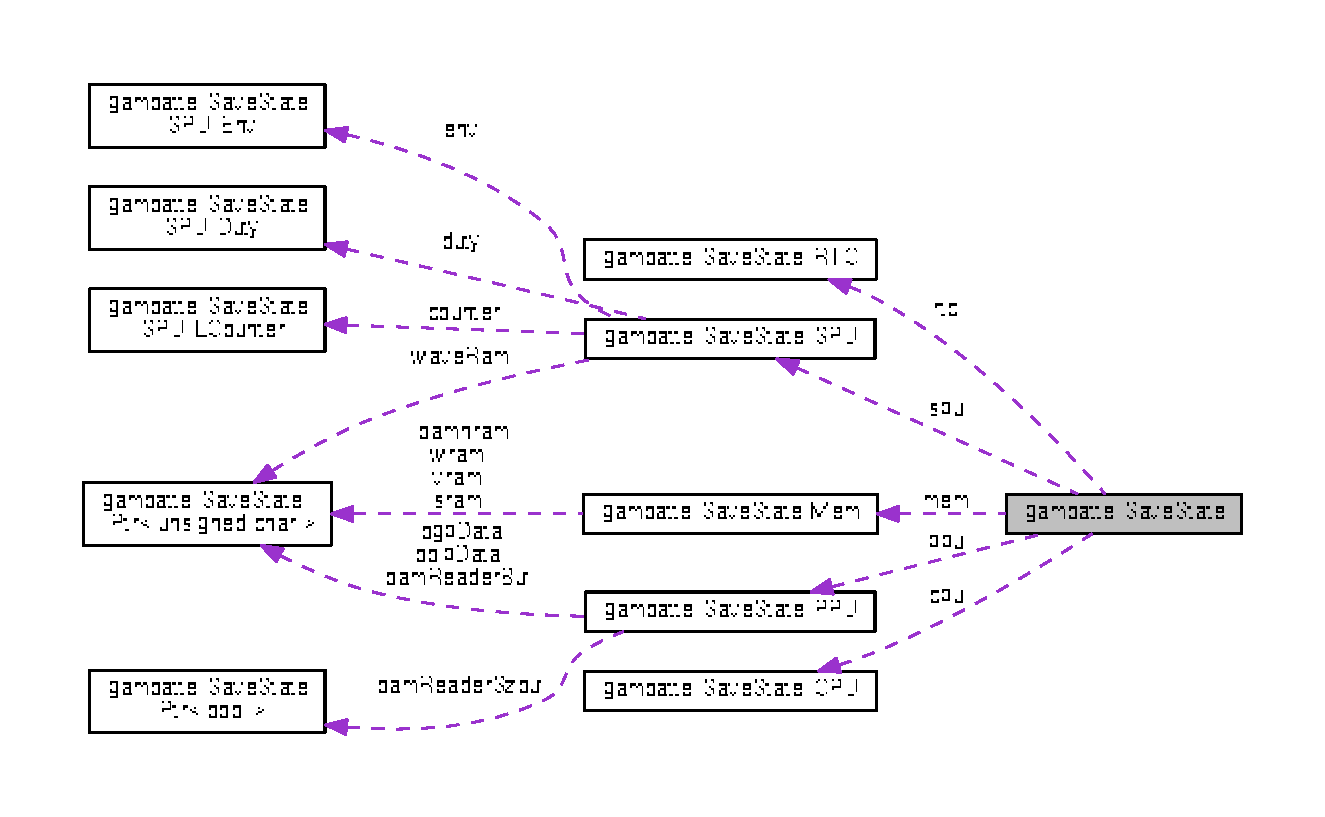
\includegraphics[width=350pt]{structgambatte_1_1SaveState__coll__graph}
\end{center}
\end{figure}
\subsection*{Classes}
\begin{DoxyCompactItemize}
\item 
struct \hyperlink{structgambatte_1_1SaveState_1_1CPU}{C\+PU}
\item 
struct \hyperlink{structgambatte_1_1SaveState_1_1Mem}{Mem}
\item 
struct \hyperlink{structgambatte_1_1SaveState_1_1PPU}{P\+PU}
\item 
class \hyperlink{classgambatte_1_1SaveState_1_1Ptr}{Ptr}
\item 
struct \hyperlink{structgambatte_1_1SaveState_1_1RTC}{R\+TC}
\item 
struct \hyperlink{structgambatte_1_1SaveState_1_1SPU}{S\+PU}
\end{DoxyCompactItemize}
\subsection*{Public Attributes}
\begin{DoxyCompactItemize}
\item 
struct \hyperlink{structgambatte_1_1SaveState_1_1CPU}{gambatte\+::\+Save\+State\+::\+C\+PU} \hyperlink{structgambatte_1_1SaveState_a6aed8b073aa20c0cd3b435994491df52}{cpu}
\item 
struct \hyperlink{structgambatte_1_1SaveState_1_1Mem}{gambatte\+::\+Save\+State\+::\+Mem} \hyperlink{structgambatte_1_1SaveState_a9ba524e9ca950531ef016734c2fc2532}{mem}
\item 
struct \hyperlink{structgambatte_1_1SaveState_1_1PPU}{gambatte\+::\+Save\+State\+::\+P\+PU} \hyperlink{structgambatte_1_1SaveState_a470cf7452cdd426d479cd337e1af1fea}{ppu}
\item 
struct \hyperlink{structgambatte_1_1SaveState_1_1SPU}{gambatte\+::\+Save\+State\+::\+S\+PU} \hyperlink{structgambatte_1_1SaveState_a0cd87c59e350952e3e12d3d2c1399d0f}{spu}
\item 
struct \hyperlink{structgambatte_1_1SaveState_1_1RTC}{gambatte\+::\+Save\+State\+::\+R\+TC} \hyperlink{structgambatte_1_1SaveState_ae9dd999c313ced5717f389cf3565556a}{rtc}
\end{DoxyCompactItemize}


\subsection{Member Data Documentation}
\mbox{\Hypertarget{structgambatte_1_1SaveState_a6aed8b073aa20c0cd3b435994491df52}\label{structgambatte_1_1SaveState_a6aed8b073aa20c0cd3b435994491df52}} 
\index{gambatte\+::\+Save\+State@{gambatte\+::\+Save\+State}!cpu@{cpu}}
\index{cpu@{cpu}!gambatte\+::\+Save\+State@{gambatte\+::\+Save\+State}}
\subsubsection{\texorpdfstring{cpu}{cpu}}
{\footnotesize\ttfamily struct \hyperlink{structgambatte_1_1SaveState_1_1CPU}{gambatte\+::\+Save\+State\+::\+C\+PU}  gambatte\+::\+Save\+State\+::cpu}

\mbox{\Hypertarget{structgambatte_1_1SaveState_a9ba524e9ca950531ef016734c2fc2532}\label{structgambatte_1_1SaveState_a9ba524e9ca950531ef016734c2fc2532}} 
\index{gambatte\+::\+Save\+State@{gambatte\+::\+Save\+State}!mem@{mem}}
\index{mem@{mem}!gambatte\+::\+Save\+State@{gambatte\+::\+Save\+State}}
\subsubsection{\texorpdfstring{mem}{mem}}
{\footnotesize\ttfamily struct \hyperlink{structgambatte_1_1SaveState_1_1Mem}{gambatte\+::\+Save\+State\+::\+Mem}  gambatte\+::\+Save\+State\+::mem}

\mbox{\Hypertarget{structgambatte_1_1SaveState_a470cf7452cdd426d479cd337e1af1fea}\label{structgambatte_1_1SaveState_a470cf7452cdd426d479cd337e1af1fea}} 
\index{gambatte\+::\+Save\+State@{gambatte\+::\+Save\+State}!ppu@{ppu}}
\index{ppu@{ppu}!gambatte\+::\+Save\+State@{gambatte\+::\+Save\+State}}
\subsubsection{\texorpdfstring{ppu}{ppu}}
{\footnotesize\ttfamily struct \hyperlink{structgambatte_1_1SaveState_1_1PPU}{gambatte\+::\+Save\+State\+::\+P\+PU}  gambatte\+::\+Save\+State\+::ppu}

\mbox{\Hypertarget{structgambatte_1_1SaveState_ae9dd999c313ced5717f389cf3565556a}\label{structgambatte_1_1SaveState_ae9dd999c313ced5717f389cf3565556a}} 
\index{gambatte\+::\+Save\+State@{gambatte\+::\+Save\+State}!rtc@{rtc}}
\index{rtc@{rtc}!gambatte\+::\+Save\+State@{gambatte\+::\+Save\+State}}
\subsubsection{\texorpdfstring{rtc}{rtc}}
{\footnotesize\ttfamily struct \hyperlink{structgambatte_1_1SaveState_1_1RTC}{gambatte\+::\+Save\+State\+::\+R\+TC}  gambatte\+::\+Save\+State\+::rtc}

\mbox{\Hypertarget{structgambatte_1_1SaveState_a0cd87c59e350952e3e12d3d2c1399d0f}\label{structgambatte_1_1SaveState_a0cd87c59e350952e3e12d3d2c1399d0f}} 
\index{gambatte\+::\+Save\+State@{gambatte\+::\+Save\+State}!spu@{spu}}
\index{spu@{spu}!gambatte\+::\+Save\+State@{gambatte\+::\+Save\+State}}
\subsubsection{\texorpdfstring{spu}{spu}}
{\footnotesize\ttfamily struct \hyperlink{structgambatte_1_1SaveState_1_1SPU}{gambatte\+::\+Save\+State\+::\+S\+PU}  gambatte\+::\+Save\+State\+::spu}



The documentation for this struct was generated from the following file\+:\begin{DoxyCompactItemize}
\item 
src/\hyperlink{savestate_8h}{savestate.\+h}\end{DoxyCompactItemize}

\hypertarget{classgambatte_1_1SoundUnit}{}\section{gambatte\+:\+:Sound\+Unit Class Reference}
\label{classgambatte_1_1SoundUnit}\index{gambatte\+::\+Sound\+Unit@{gambatte\+::\+Sound\+Unit}}


{\ttfamily \#include $<$sound\+\_\+unit.\+h$>$}



Inheritance diagram for gambatte\+:\+:Sound\+Unit\+:
\nopagebreak
\begin{figure}[H]
\begin{center}
\leavevmode
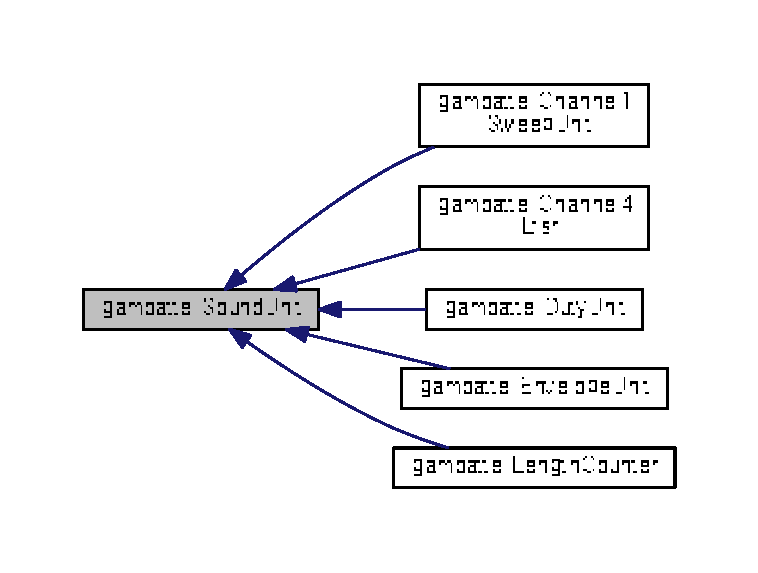
\includegraphics[width=350pt]{classgambatte_1_1SoundUnit__inherit__graph}
\end{center}
\end{figure}
\subsection*{Public Types}
\begin{DoxyCompactItemize}
\item 
enum \{ \hyperlink{classgambatte_1_1SoundUnit_a42980887d13053bdf6dfbdbece460ff8a9b3f5f9a9fb3bac559e001d5f0d3fff8}{counter\+\_\+max} = 0x80000000u, 
\hyperlink{classgambatte_1_1SoundUnit_a42980887d13053bdf6dfbdbece460ff8a0aa17344792e01301389d1a0fbe9a159}{counter\+\_\+disabled} = 0x\+F\+F\+F\+F\+F\+F\+F\+Fu
 \}
\end{DoxyCompactItemize}
\subsection*{Public Member Functions}
\begin{DoxyCompactItemize}
\item 
virtual \hyperlink{classgambatte_1_1SoundUnit_a4eee8be8027fbbc20a13bfe27b68f74a}{$\sim$\+Sound\+Unit} ()
\item 
virtual void \hyperlink{classgambatte_1_1SoundUnit_a8ad6df87fc3700d9d3bee470383197b4}{event} ()=0
\item 
void \hyperlink{classgambatte_1_1SoundUnit_a3f33fea3fbb7987029b74cbc64d7668f}{load\+Or\+Save2} (\hyperlink{classgambatte_1_1loadsave}{loadsave} \&\hyperlink{ppu_8cpp_a2f2eca6997ee7baf8901725ae074d45b}{state})
\item 
virtual void \hyperlink{classgambatte_1_1SoundUnit_a3baa270f75463b24cd79fe5970103d4f}{reset\+Counters} (unsigned)
\item 
unsigned \hyperlink{classgambatte_1_1SoundUnit_acad13952e5b24b3bc05b9aa42c8b9249}{counter} () const
\end{DoxyCompactItemize}
\subsection*{Protected Member Functions}
\begin{DoxyCompactItemize}
\item 
\hyperlink{classgambatte_1_1SoundUnit_ab5bdb53bbf42d92d6d47db012aec1577}{Sound\+Unit} ()
\end{DoxyCompactItemize}
\subsection*{Protected Attributes}
\begin{DoxyCompactItemize}
\item 
unsigned \hyperlink{classgambatte_1_1SoundUnit_a06297f078dca7d403648ce3455a790be}{counter\+\_\+}
\end{DoxyCompactItemize}


\subsection{Member Enumeration Documentation}
\mbox{\Hypertarget{classgambatte_1_1SoundUnit_a42980887d13053bdf6dfbdbece460ff8}\label{classgambatte_1_1SoundUnit_a42980887d13053bdf6dfbdbece460ff8}} 
\subsubsection{\texorpdfstring{anonymous enum}{anonymous enum}}
{\footnotesize\ttfamily anonymous enum}

\begin{DoxyEnumFields}{Enumerator}
\raisebox{\heightof{T}}[0pt][0pt]{\index{counter\+\_\+max@{counter\+\_\+max}!gambatte\+::\+Sound\+Unit@{gambatte\+::\+Sound\+Unit}}\index{gambatte\+::\+Sound\+Unit@{gambatte\+::\+Sound\+Unit}!counter\+\_\+max@{counter\+\_\+max}}}\mbox{\Hypertarget{classgambatte_1_1SoundUnit_a42980887d13053bdf6dfbdbece460ff8a9b3f5f9a9fb3bac559e001d5f0d3fff8}\label{classgambatte_1_1SoundUnit_a42980887d13053bdf6dfbdbece460ff8a9b3f5f9a9fb3bac559e001d5f0d3fff8}} 
counter\+\_\+max&\\
\hline

\raisebox{\heightof{T}}[0pt][0pt]{\index{counter\+\_\+disabled@{counter\+\_\+disabled}!gambatte\+::\+Sound\+Unit@{gambatte\+::\+Sound\+Unit}}\index{gambatte\+::\+Sound\+Unit@{gambatte\+::\+Sound\+Unit}!counter\+\_\+disabled@{counter\+\_\+disabled}}}\mbox{\Hypertarget{classgambatte_1_1SoundUnit_a42980887d13053bdf6dfbdbece460ff8a0aa17344792e01301389d1a0fbe9a159}\label{classgambatte_1_1SoundUnit_a42980887d13053bdf6dfbdbece460ff8a0aa17344792e01301389d1a0fbe9a159}} 
counter\+\_\+disabled&\\
\hline

\end{DoxyEnumFields}


\subsection{Constructor \& Destructor Documentation}
\mbox{\Hypertarget{classgambatte_1_1SoundUnit_a4eee8be8027fbbc20a13bfe27b68f74a}\label{classgambatte_1_1SoundUnit_a4eee8be8027fbbc20a13bfe27b68f74a}} 
\index{gambatte\+::\+Sound\+Unit@{gambatte\+::\+Sound\+Unit}!````~Sound\+Unit@{$\sim$\+Sound\+Unit}}
\index{````~Sound\+Unit@{$\sim$\+Sound\+Unit}!gambatte\+::\+Sound\+Unit@{gambatte\+::\+Sound\+Unit}}
\subsubsection{\texorpdfstring{$\sim$\+Sound\+Unit()}{~SoundUnit()}}
{\footnotesize\ttfamily virtual gambatte\+::\+Sound\+Unit\+::$\sim$\+Sound\+Unit (\begin{DoxyParamCaption}{ }\end{DoxyParamCaption})\hspace{0.3cm}{\ttfamily [inline]}, {\ttfamily [virtual]}}

\mbox{\Hypertarget{classgambatte_1_1SoundUnit_ab5bdb53bbf42d92d6d47db012aec1577}\label{classgambatte_1_1SoundUnit_ab5bdb53bbf42d92d6d47db012aec1577}} 
\index{gambatte\+::\+Sound\+Unit@{gambatte\+::\+Sound\+Unit}!Sound\+Unit@{Sound\+Unit}}
\index{Sound\+Unit@{Sound\+Unit}!gambatte\+::\+Sound\+Unit@{gambatte\+::\+Sound\+Unit}}
\subsubsection{\texorpdfstring{Sound\+Unit()}{SoundUnit()}}
{\footnotesize\ttfamily gambatte\+::\+Sound\+Unit\+::\+Sound\+Unit (\begin{DoxyParamCaption}{ }\end{DoxyParamCaption})\hspace{0.3cm}{\ttfamily [inline]}, {\ttfamily [protected]}}



\subsection{Member Function Documentation}
\mbox{\Hypertarget{classgambatte_1_1SoundUnit_acad13952e5b24b3bc05b9aa42c8b9249}\label{classgambatte_1_1SoundUnit_acad13952e5b24b3bc05b9aa42c8b9249}} 
\index{gambatte\+::\+Sound\+Unit@{gambatte\+::\+Sound\+Unit}!counter@{counter}}
\index{counter@{counter}!gambatte\+::\+Sound\+Unit@{gambatte\+::\+Sound\+Unit}}
\subsubsection{\texorpdfstring{counter()}{counter()}}
{\footnotesize\ttfamily unsigned gambatte\+::\+Sound\+Unit\+::counter (\begin{DoxyParamCaption}{ }\end{DoxyParamCaption}) const\hspace{0.3cm}{\ttfamily [inline]}}

\mbox{\Hypertarget{classgambatte_1_1SoundUnit_a8ad6df87fc3700d9d3bee470383197b4}\label{classgambatte_1_1SoundUnit_a8ad6df87fc3700d9d3bee470383197b4}} 
\index{gambatte\+::\+Sound\+Unit@{gambatte\+::\+Sound\+Unit}!event@{event}}
\index{event@{event}!gambatte\+::\+Sound\+Unit@{gambatte\+::\+Sound\+Unit}}
\subsubsection{\texorpdfstring{event()}{event()}}
{\footnotesize\ttfamily virtual void gambatte\+::\+Sound\+Unit\+::event (\begin{DoxyParamCaption}{ }\end{DoxyParamCaption})\hspace{0.3cm}{\ttfamily [pure virtual]}}



Implemented in \hyperlink{classgambatte_1_1Channel1_1_1SweepUnit_a17c182372fc3f4aaf845ab89cf20201d}{gambatte\+::\+Channel1\+::\+Sweep\+Unit}, \hyperlink{classgambatte_1_1Channel4_1_1Lfsr_a019ab6fad6c598fdc6f061b70df93fdc}{gambatte\+::\+Channel4\+::\+Lfsr}, \hyperlink{classgambatte_1_1EnvelopeUnit_a9273d36ce1ef6e3e11a4d2bb0d3bc367}{gambatte\+::\+Envelope\+Unit}, \hyperlink{classgambatte_1_1LengthCounter_ab0d3eda374d487f8a0b79ea447cca91a}{gambatte\+::\+Length\+Counter}, and \hyperlink{classgambatte_1_1DutyUnit_a2f051bb4772d30c58f2e88b85e947e61}{gambatte\+::\+Duty\+Unit}.

\mbox{\Hypertarget{classgambatte_1_1SoundUnit_a3f33fea3fbb7987029b74cbc64d7668f}\label{classgambatte_1_1SoundUnit_a3f33fea3fbb7987029b74cbc64d7668f}} 
\index{gambatte\+::\+Sound\+Unit@{gambatte\+::\+Sound\+Unit}!load\+Or\+Save2@{load\+Or\+Save2}}
\index{load\+Or\+Save2@{load\+Or\+Save2}!gambatte\+::\+Sound\+Unit@{gambatte\+::\+Sound\+Unit}}
\subsubsection{\texorpdfstring{load\+Or\+Save2()}{loadOrSave2()}}
{\footnotesize\ttfamily void gambatte\+::\+Sound\+Unit\+::load\+Or\+Save2 (\begin{DoxyParamCaption}\item[{\hyperlink{classgambatte_1_1loadsave}{loadsave} \&}]{state }\end{DoxyParamCaption})\hspace{0.3cm}{\ttfamily [inline]}}

\mbox{\Hypertarget{classgambatte_1_1SoundUnit_a3baa270f75463b24cd79fe5970103d4f}\label{classgambatte_1_1SoundUnit_a3baa270f75463b24cd79fe5970103d4f}} 
\index{gambatte\+::\+Sound\+Unit@{gambatte\+::\+Sound\+Unit}!reset\+Counters@{reset\+Counters}}
\index{reset\+Counters@{reset\+Counters}!gambatte\+::\+Sound\+Unit@{gambatte\+::\+Sound\+Unit}}
\subsubsection{\texorpdfstring{reset\+Counters()}{resetCounters()}}
{\footnotesize\ttfamily virtual void gambatte\+::\+Sound\+Unit\+::reset\+Counters (\begin{DoxyParamCaption}\item[{unsigned}]{ }\end{DoxyParamCaption})\hspace{0.3cm}{\ttfamily [inline]}, {\ttfamily [virtual]}}



Reimplemented in \hyperlink{classgambatte_1_1Channel4_1_1Lfsr_acdeb93a45132b45567f97878ed6306b9}{gambatte\+::\+Channel4\+::\+Lfsr}, and \hyperlink{classgambatte_1_1DutyUnit_a69b982611026639129fda42e637e7b12}{gambatte\+::\+Duty\+Unit}.



\subsection{Member Data Documentation}
\mbox{\Hypertarget{classgambatte_1_1SoundUnit_a06297f078dca7d403648ce3455a790be}\label{classgambatte_1_1SoundUnit_a06297f078dca7d403648ce3455a790be}} 
\index{gambatte\+::\+Sound\+Unit@{gambatte\+::\+Sound\+Unit}!counter\+\_\+@{counter\+\_\+}}
\index{counter\+\_\+@{counter\+\_\+}!gambatte\+::\+Sound\+Unit@{gambatte\+::\+Sound\+Unit}}
\subsubsection{\texorpdfstring{counter\+\_\+}{counter\_}}
{\footnotesize\ttfamily unsigned gambatte\+::\+Sound\+Unit\+::counter\+\_\+\hspace{0.3cm}{\ttfamily [protected]}}



The documentation for this class was generated from the following file\+:\begin{DoxyCompactItemize}
\item 
src/sound/\hyperlink{sound__unit_8h}{sound\+\_\+unit.\+h}\end{DoxyCompactItemize}

\hypertarget{structgambatte_1_1PPUPriv_1_1Sprite}{}\section{gambatte\+:\+:P\+P\+U\+Priv\+:\+:Sprite Struct Reference}
\label{structgambatte_1_1PPUPriv_1_1Sprite}\index{gambatte\+::\+P\+P\+U\+Priv\+::\+Sprite@{gambatte\+::\+P\+P\+U\+Priv\+::\+Sprite}}


{\ttfamily \#include $<$ppu.\+h$>$}

\subsection*{Public Member Functions}
\begin{DoxyCompactItemize}
\item 
void \hyperlink{structgambatte_1_1PPUPriv_1_1Sprite_a9e3b7d2d3bbbe17ca3e23480a2afa28c}{load\+Or\+Save} (\hyperlink{classgambatte_1_1loadsave}{loadsave} \&\hyperlink{ppu_8cpp_a2f2eca6997ee7baf8901725ae074d45b}{state})
\end{DoxyCompactItemize}
\subsection*{Public Attributes}
\begin{DoxyCompactItemize}
\item 
unsigned char \hyperlink{structgambatte_1_1PPUPriv_1_1Sprite_aa9f6c5acaecae4ca4ab8521616ae7036}{spx}
\item 
unsigned char \hyperlink{structgambatte_1_1PPUPriv_1_1Sprite_ac20457cc822cd213068bc2264fccf2d0}{oampos}
\item 
unsigned char \hyperlink{structgambatte_1_1PPUPriv_1_1Sprite_a720b7dfab129094396cf8903bd39b05e}{line}
\item 
unsigned char \hyperlink{structgambatte_1_1PPUPriv_1_1Sprite_aa748bc273a1fff5841f04f4bd18ebd6b}{attrib}
\end{DoxyCompactItemize}


\subsection{Member Function Documentation}
\mbox{\Hypertarget{structgambatte_1_1PPUPriv_1_1Sprite_a9e3b7d2d3bbbe17ca3e23480a2afa28c}\label{structgambatte_1_1PPUPriv_1_1Sprite_a9e3b7d2d3bbbe17ca3e23480a2afa28c}} 
\index{gambatte\+::\+P\+P\+U\+Priv\+::\+Sprite@{gambatte\+::\+P\+P\+U\+Priv\+::\+Sprite}!load\+Or\+Save@{load\+Or\+Save}}
\index{load\+Or\+Save@{load\+Or\+Save}!gambatte\+::\+P\+P\+U\+Priv\+::\+Sprite@{gambatte\+::\+P\+P\+U\+Priv\+::\+Sprite}}
\subsubsection{\texorpdfstring{load\+Or\+Save()}{loadOrSave()}}
{\footnotesize\ttfamily void gambatte\+::\+P\+P\+U\+Priv\+::\+Sprite\+::load\+Or\+Save (\begin{DoxyParamCaption}\item[{\hyperlink{classgambatte_1_1loadsave}{loadsave} \&}]{state }\end{DoxyParamCaption})\hspace{0.3cm}{\ttfamily [inline]}}



\subsection{Member Data Documentation}
\mbox{\Hypertarget{structgambatte_1_1PPUPriv_1_1Sprite_aa748bc273a1fff5841f04f4bd18ebd6b}\label{structgambatte_1_1PPUPriv_1_1Sprite_aa748bc273a1fff5841f04f4bd18ebd6b}} 
\index{gambatte\+::\+P\+P\+U\+Priv\+::\+Sprite@{gambatte\+::\+P\+P\+U\+Priv\+::\+Sprite}!attrib@{attrib}}
\index{attrib@{attrib}!gambatte\+::\+P\+P\+U\+Priv\+::\+Sprite@{gambatte\+::\+P\+P\+U\+Priv\+::\+Sprite}}
\subsubsection{\texorpdfstring{attrib}{attrib}}
{\footnotesize\ttfamily unsigned char gambatte\+::\+P\+P\+U\+Priv\+::\+Sprite\+::attrib}

\mbox{\Hypertarget{structgambatte_1_1PPUPriv_1_1Sprite_a720b7dfab129094396cf8903bd39b05e}\label{structgambatte_1_1PPUPriv_1_1Sprite_a720b7dfab129094396cf8903bd39b05e}} 
\index{gambatte\+::\+P\+P\+U\+Priv\+::\+Sprite@{gambatte\+::\+P\+P\+U\+Priv\+::\+Sprite}!line@{line}}
\index{line@{line}!gambatte\+::\+P\+P\+U\+Priv\+::\+Sprite@{gambatte\+::\+P\+P\+U\+Priv\+::\+Sprite}}
\subsubsection{\texorpdfstring{line}{line}}
{\footnotesize\ttfamily unsigned char gambatte\+::\+P\+P\+U\+Priv\+::\+Sprite\+::line}

\mbox{\Hypertarget{structgambatte_1_1PPUPriv_1_1Sprite_ac20457cc822cd213068bc2264fccf2d0}\label{structgambatte_1_1PPUPriv_1_1Sprite_ac20457cc822cd213068bc2264fccf2d0}} 
\index{gambatte\+::\+P\+P\+U\+Priv\+::\+Sprite@{gambatte\+::\+P\+P\+U\+Priv\+::\+Sprite}!oampos@{oampos}}
\index{oampos@{oampos}!gambatte\+::\+P\+P\+U\+Priv\+::\+Sprite@{gambatte\+::\+P\+P\+U\+Priv\+::\+Sprite}}
\subsubsection{\texorpdfstring{oampos}{oampos}}
{\footnotesize\ttfamily unsigned char gambatte\+::\+P\+P\+U\+Priv\+::\+Sprite\+::oampos}

\mbox{\Hypertarget{structgambatte_1_1PPUPriv_1_1Sprite_aa9f6c5acaecae4ca4ab8521616ae7036}\label{structgambatte_1_1PPUPriv_1_1Sprite_aa9f6c5acaecae4ca4ab8521616ae7036}} 
\index{gambatte\+::\+P\+P\+U\+Priv\+::\+Sprite@{gambatte\+::\+P\+P\+U\+Priv\+::\+Sprite}!spx@{spx}}
\index{spx@{spx}!gambatte\+::\+P\+P\+U\+Priv\+::\+Sprite@{gambatte\+::\+P\+P\+U\+Priv\+::\+Sprite}}
\subsubsection{\texorpdfstring{spx}{spx}}
{\footnotesize\ttfamily unsigned char gambatte\+::\+P\+P\+U\+Priv\+::\+Sprite\+::spx}



The documentation for this struct was generated from the following file\+:\begin{DoxyCompactItemize}
\item 
src/video/\hyperlink{ppu_8h}{ppu.\+h}\end{DoxyCompactItemize}

\hypertarget{classgambatte_1_1SpriteMapper}{}\section{gambatte\+:\+:Sprite\+Mapper Class Reference}
\label{classgambatte_1_1SpriteMapper}\index{gambatte\+::\+Sprite\+Mapper@{gambatte\+::\+Sprite\+Mapper}}


{\ttfamily \#include $<$sprite\+\_\+mapper.\+h$>$}



Collaboration diagram for gambatte\+:\+:Sprite\+Mapper\+:
\nopagebreak
\begin{figure}[H]
\begin{center}
\leavevmode
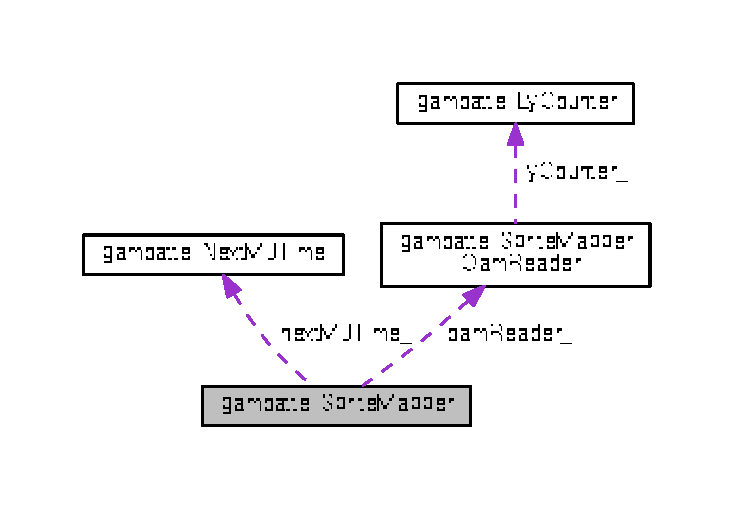
\includegraphics[width=350pt]{classgambatte_1_1SpriteMapper__coll__graph}
\end{center}
\end{figure}
\subsection*{Classes}
\begin{DoxyCompactItemize}
\item 
class \hyperlink{classgambatte_1_1SpriteMapper_1_1OamReader}{Oam\+Reader}
\end{DoxyCompactItemize}
\subsection*{Public Member Functions}
\begin{DoxyCompactItemize}
\item 
\hyperlink{classgambatte_1_1SpriteMapper_afa54d28e21f1ff73031a387fb8aefdce}{Sprite\+Mapper} (\hyperlink{classgambatte_1_1NextM0Time}{Next\+M0\+Time} \&next\+M0\+Time, \hyperlink{classgambatte_1_1LyCounter}{Ly\+Counter} const \&ly\+Counter, unsigned char const $\ast$\hyperlink{classgambatte_1_1SpriteMapper_a558ee1ff5817b79285f7cc91d627535b}{oamram})
\item 
void \hyperlink{classgambatte_1_1SpriteMapper_a30a75a0ef5dcae59f55152515a967843}{reset} (unsigned char const $\ast$\hyperlink{classgambatte_1_1SpriteMapper_a558ee1ff5817b79285f7cc91d627535b}{oamram}, bool cgb)
\item 
unsigned \hyperlink{classgambatte_1_1SpriteMapper_a1dc90dda342bb3587d91a763a35c9a79}{do\+Event} (unsigned time)
\item 
bool \hyperlink{classgambatte_1_1SpriteMapper_ad67ee3b9b5c1f188ba33f5716a3f5853}{large\+Sprites} (unsigned sp\+No) const
\item 
unsigned \hyperlink{classgambatte_1_1SpriteMapper_ad44d62550eb865da721b1092539647e8}{num\+Sprites} (unsigned \hyperlink{video_8cpp_ab1c1cf762ec2da5588c30a13cd60af91}{ly}) const
\item 
void \hyperlink{classgambatte_1_1SpriteMapper_a899e21a4d6356b9c3587872eb290d035}{oam\+Change} (unsigned cc)
\item 
void \hyperlink{classgambatte_1_1SpriteMapper_aa090796deeec5896abfeb6b5dfc41045}{oam\+Change} (unsigned char const $\ast$\hyperlink{classgambatte_1_1SpriteMapper_a558ee1ff5817b79285f7cc91d627535b}{oamram}, unsigned cc)
\item 
unsigned char const  $\ast$ \hyperlink{classgambatte_1_1SpriteMapper_a558ee1ff5817b79285f7cc91d627535b}{oamram} () const
\item 
unsigned char const  $\ast$ \hyperlink{classgambatte_1_1SpriteMapper_a9f316f5fb82169de7855d56d2446b793}{posbuf} () const
\item 
void \hyperlink{classgambatte_1_1SpriteMapper_a08aeaf6bb42e440b9f7f4066366b673b}{pre\+Speed\+Change} (unsigned cc)
\item 
void \hyperlink{classgambatte_1_1SpriteMapper_a20063931c4c6144769d9ce4c064fb374}{post\+Speed\+Change} (unsigned cc)
\item 
void \hyperlink{classgambatte_1_1SpriteMapper_ad59a63b416f0c800bde4e29a5bf73483}{reset\+Cycle\+Counter} (unsigned old\+Cc, unsigned new\+Cc)
\item 
void \hyperlink{classgambatte_1_1SpriteMapper_a8b2c5932b622da5cac4293564295c84d}{set\+Large\+Sprites\+Source} (bool src)
\item 
unsigned char const  $\ast$ \hyperlink{classgambatte_1_1SpriteMapper_a8db6c630bc151ddc188259a88faa069d}{sprites} (unsigned \hyperlink{video_8cpp_ab1c1cf762ec2da5588c30a13cd60af91}{ly}) const
\item 
void \hyperlink{classgambatte_1_1SpriteMapper_a6121ec198af413d2609ef0269f7e1984}{set\+State\+Ptrs} (\hyperlink{structgambatte_1_1SaveState}{Save\+State} \&\hyperlink{ppu_8cpp_a2f2eca6997ee7baf8901725ae074d45b}{state})
\item 
void \hyperlink{classgambatte_1_1SpriteMapper_a4bea9956005c54e0595d2700157a1394}{enable\+Display} (unsigned cc)
\item 
void \hyperlink{classgambatte_1_1SpriteMapper_a0bf6bfd50a86c4675d9ef040870dde9c}{save\+State} (\hyperlink{structgambatte_1_1SaveState}{Save\+State} \&\hyperlink{ppu_8cpp_a2f2eca6997ee7baf8901725ae074d45b}{state}) const
\item 
void \hyperlink{classgambatte_1_1SpriteMapper_a0d629b8f37f68686b87ccaeb8f62dff1}{load\+State} (\hyperlink{structgambatte_1_1SaveState}{Save\+State} const \&\hyperlink{ppu_8cpp_a2f2eca6997ee7baf8901725ae074d45b}{state}, unsigned char const $\ast$\hyperlink{classgambatte_1_1SpriteMapper_a558ee1ff5817b79285f7cc91d627535b}{oamram})
\item 
bool \hyperlink{classgambatte_1_1SpriteMapper_abf83b02b1345c60a560c60a119d87117}{inactive\+Period\+After\+Display\+Enable} (unsigned cc) const
\item 
void \hyperlink{classgambatte_1_1SpriteMapper_a9bda0d2b7ebd6a884dc5a7aea82f2944}{load\+Or\+Save} (\hyperlink{classgambatte_1_1loadsave}{loadsave} \&\hyperlink{ppu_8cpp_a2f2eca6997ee7baf8901725ae074d45b}{state})
\end{DoxyCompactItemize}
\subsection*{Static Public Member Functions}
\begin{DoxyCompactItemize}
\item 
static unsigned \hyperlink{classgambatte_1_1SpriteMapper_afb35f1ed6b01680065e0c9ba7dca73bc}{schedule} (\hyperlink{classgambatte_1_1LyCounter}{Ly\+Counter} const \&ly\+Counter, unsigned cc)
\end{DoxyCompactItemize}
\subsection*{Private Types}
\begin{DoxyCompactItemize}
\item 
enum \{ \hyperlink{classgambatte_1_1SpriteMapper_a523804247b052cc0c961255e4dd20ce8af390b53d20749943c37e1f9c84a9a01e}{need\+\_\+sorting\+\_\+mask} = 0x80
 \}
\end{DoxyCompactItemize}
\subsection*{Private Member Functions}
\begin{DoxyCompactItemize}
\item 
void \hyperlink{classgambatte_1_1SpriteMapper_a65e513f3c368d2ba0dac2a9625edc57a}{clear\+Map} ()
\item 
void \hyperlink{classgambatte_1_1SpriteMapper_a98f85e5f98730495f6a1648268f03a2a}{map\+Sprites} ()
\item 
void \hyperlink{classgambatte_1_1SpriteMapper_aeaa3e4b1f02ec1f6a4fc99d0dd44a54b}{sort\+Line} (unsigned \hyperlink{video_8cpp_ab1c1cf762ec2da5588c30a13cd60af91}{ly}) const
\end{DoxyCompactItemize}
\subsection*{Private Attributes}
\begin{DoxyCompactItemize}
\item 
unsigned char \hyperlink{classgambatte_1_1SpriteMapper_aaf20b8b09e7eabc2ad3051b4bcbb7470}{spritemap\+\_\+} \mbox{[}144 $\ast$10\mbox{]}
\item 
unsigned char \hyperlink{classgambatte_1_1SpriteMapper_a8208222a16c3164b7b8de51cfc0e7727}{num\+\_\+} \mbox{[}144\mbox{]}
\item 
\hyperlink{classgambatte_1_1NextM0Time}{Next\+M0\+Time} \& \hyperlink{classgambatte_1_1SpriteMapper_ab953c5641f686e70c1ff6114ed8d12fa}{next\+M0\+Time\+\_\+}
\item 
\hyperlink{classgambatte_1_1SpriteMapper_1_1OamReader}{Oam\+Reader} \hyperlink{classgambatte_1_1SpriteMapper_a66612bed9813c478ed12879b6c8afd4a}{oam\+Reader\+\_\+}
\end{DoxyCompactItemize}


\subsection{Member Enumeration Documentation}
\mbox{\Hypertarget{classgambatte_1_1SpriteMapper_a523804247b052cc0c961255e4dd20ce8}\label{classgambatte_1_1SpriteMapper_a523804247b052cc0c961255e4dd20ce8}} 
\subsubsection{\texorpdfstring{anonymous enum}{anonymous enum}}
{\footnotesize\ttfamily anonymous enum\hspace{0.3cm}{\ttfamily [private]}}

\begin{DoxyEnumFields}{Enumerator}
\raisebox{\heightof{T}}[0pt][0pt]{\index{need\+\_\+sorting\+\_\+mask@{need\+\_\+sorting\+\_\+mask}!gambatte\+::\+Sprite\+Mapper@{gambatte\+::\+Sprite\+Mapper}}\index{gambatte\+::\+Sprite\+Mapper@{gambatte\+::\+Sprite\+Mapper}!need\+\_\+sorting\+\_\+mask@{need\+\_\+sorting\+\_\+mask}}}\mbox{\Hypertarget{classgambatte_1_1SpriteMapper_a523804247b052cc0c961255e4dd20ce8af390b53d20749943c37e1f9c84a9a01e}\label{classgambatte_1_1SpriteMapper_a523804247b052cc0c961255e4dd20ce8af390b53d20749943c37e1f9c84a9a01e}} 
need\+\_\+sorting\+\_\+mask&\\
\hline

\end{DoxyEnumFields}


\subsection{Constructor \& Destructor Documentation}
\mbox{\Hypertarget{classgambatte_1_1SpriteMapper_afa54d28e21f1ff73031a387fb8aefdce}\label{classgambatte_1_1SpriteMapper_afa54d28e21f1ff73031a387fb8aefdce}} 
\index{gambatte\+::\+Sprite\+Mapper@{gambatte\+::\+Sprite\+Mapper}!Sprite\+Mapper@{Sprite\+Mapper}}
\index{Sprite\+Mapper@{Sprite\+Mapper}!gambatte\+::\+Sprite\+Mapper@{gambatte\+::\+Sprite\+Mapper}}
\subsubsection{\texorpdfstring{Sprite\+Mapper()}{SpriteMapper()}}
{\footnotesize\ttfamily gambatte\+::\+Sprite\+Mapper\+::\+Sprite\+Mapper (\begin{DoxyParamCaption}\item[{\hyperlink{classgambatte_1_1NextM0Time}{Next\+M0\+Time} \&}]{next\+M0\+Time,  }\item[{\hyperlink{classgambatte_1_1LyCounter}{Ly\+Counter} const \&}]{ly\+Counter,  }\item[{unsigned char const $\ast$}]{oamram }\end{DoxyParamCaption})}



\subsection{Member Function Documentation}
\mbox{\Hypertarget{classgambatte_1_1SpriteMapper_a65e513f3c368d2ba0dac2a9625edc57a}\label{classgambatte_1_1SpriteMapper_a65e513f3c368d2ba0dac2a9625edc57a}} 
\index{gambatte\+::\+Sprite\+Mapper@{gambatte\+::\+Sprite\+Mapper}!clear\+Map@{clear\+Map}}
\index{clear\+Map@{clear\+Map}!gambatte\+::\+Sprite\+Mapper@{gambatte\+::\+Sprite\+Mapper}}
\subsubsection{\texorpdfstring{clear\+Map()}{clearMap()}}
{\footnotesize\ttfamily void gambatte\+::\+Sprite\+Mapper\+::clear\+Map (\begin{DoxyParamCaption}{ }\end{DoxyParamCaption})\hspace{0.3cm}{\ttfamily [private]}}

\mbox{\Hypertarget{classgambatte_1_1SpriteMapper_a1dc90dda342bb3587d91a763a35c9a79}\label{classgambatte_1_1SpriteMapper_a1dc90dda342bb3587d91a763a35c9a79}} 
\index{gambatte\+::\+Sprite\+Mapper@{gambatte\+::\+Sprite\+Mapper}!do\+Event@{do\+Event}}
\index{do\+Event@{do\+Event}!gambatte\+::\+Sprite\+Mapper@{gambatte\+::\+Sprite\+Mapper}}
\subsubsection{\texorpdfstring{do\+Event()}{doEvent()}}
{\footnotesize\ttfamily unsigned gambatte\+::\+Sprite\+Mapper\+::do\+Event (\begin{DoxyParamCaption}\item[{unsigned}]{time }\end{DoxyParamCaption})}

\mbox{\Hypertarget{classgambatte_1_1SpriteMapper_a4bea9956005c54e0595d2700157a1394}\label{classgambatte_1_1SpriteMapper_a4bea9956005c54e0595d2700157a1394}} 
\index{gambatte\+::\+Sprite\+Mapper@{gambatte\+::\+Sprite\+Mapper}!enable\+Display@{enable\+Display}}
\index{enable\+Display@{enable\+Display}!gambatte\+::\+Sprite\+Mapper@{gambatte\+::\+Sprite\+Mapper}}
\subsubsection{\texorpdfstring{enable\+Display()}{enableDisplay()}}
{\footnotesize\ttfamily void gambatte\+::\+Sprite\+Mapper\+::enable\+Display (\begin{DoxyParamCaption}\item[{unsigned}]{cc }\end{DoxyParamCaption})\hspace{0.3cm}{\ttfamily [inline]}}

\mbox{\Hypertarget{classgambatte_1_1SpriteMapper_abf83b02b1345c60a560c60a119d87117}\label{classgambatte_1_1SpriteMapper_abf83b02b1345c60a560c60a119d87117}} 
\index{gambatte\+::\+Sprite\+Mapper@{gambatte\+::\+Sprite\+Mapper}!inactive\+Period\+After\+Display\+Enable@{inactive\+Period\+After\+Display\+Enable}}
\index{inactive\+Period\+After\+Display\+Enable@{inactive\+Period\+After\+Display\+Enable}!gambatte\+::\+Sprite\+Mapper@{gambatte\+::\+Sprite\+Mapper}}
\subsubsection{\texorpdfstring{inactive\+Period\+After\+Display\+Enable()}{inactivePeriodAfterDisplayEnable()}}
{\footnotesize\ttfamily bool gambatte\+::\+Sprite\+Mapper\+::inactive\+Period\+After\+Display\+Enable (\begin{DoxyParamCaption}\item[{unsigned}]{cc }\end{DoxyParamCaption}) const\hspace{0.3cm}{\ttfamily [inline]}}

\mbox{\Hypertarget{classgambatte_1_1SpriteMapper_ad67ee3b9b5c1f188ba33f5716a3f5853}\label{classgambatte_1_1SpriteMapper_ad67ee3b9b5c1f188ba33f5716a3f5853}} 
\index{gambatte\+::\+Sprite\+Mapper@{gambatte\+::\+Sprite\+Mapper}!large\+Sprites@{large\+Sprites}}
\index{large\+Sprites@{large\+Sprites}!gambatte\+::\+Sprite\+Mapper@{gambatte\+::\+Sprite\+Mapper}}
\subsubsection{\texorpdfstring{large\+Sprites()}{largeSprites()}}
{\footnotesize\ttfamily bool gambatte\+::\+Sprite\+Mapper\+::large\+Sprites (\begin{DoxyParamCaption}\item[{unsigned}]{sp\+No }\end{DoxyParamCaption}) const\hspace{0.3cm}{\ttfamily [inline]}}

\mbox{\Hypertarget{classgambatte_1_1SpriteMapper_a9bda0d2b7ebd6a884dc5a7aea82f2944}\label{classgambatte_1_1SpriteMapper_a9bda0d2b7ebd6a884dc5a7aea82f2944}} 
\index{gambatte\+::\+Sprite\+Mapper@{gambatte\+::\+Sprite\+Mapper}!load\+Or\+Save@{load\+Or\+Save}}
\index{load\+Or\+Save@{load\+Or\+Save}!gambatte\+::\+Sprite\+Mapper@{gambatte\+::\+Sprite\+Mapper}}
\subsubsection{\texorpdfstring{load\+Or\+Save()}{loadOrSave()}}
{\footnotesize\ttfamily void gambatte\+::\+Sprite\+Mapper\+::load\+Or\+Save (\begin{DoxyParamCaption}\item[{\hyperlink{classgambatte_1_1loadsave}{loadsave} \&}]{state }\end{DoxyParamCaption})\hspace{0.3cm}{\ttfamily [inline]}}

\mbox{\Hypertarget{classgambatte_1_1SpriteMapper_a0d629b8f37f68686b87ccaeb8f62dff1}\label{classgambatte_1_1SpriteMapper_a0d629b8f37f68686b87ccaeb8f62dff1}} 
\index{gambatte\+::\+Sprite\+Mapper@{gambatte\+::\+Sprite\+Mapper}!load\+State@{load\+State}}
\index{load\+State@{load\+State}!gambatte\+::\+Sprite\+Mapper@{gambatte\+::\+Sprite\+Mapper}}
\subsubsection{\texorpdfstring{load\+State()}{loadState()}}
{\footnotesize\ttfamily void gambatte\+::\+Sprite\+Mapper\+::load\+State (\begin{DoxyParamCaption}\item[{\hyperlink{structgambatte_1_1SaveState}{Save\+State} const \&}]{state,  }\item[{unsigned char const $\ast$}]{oamram }\end{DoxyParamCaption})\hspace{0.3cm}{\ttfamily [inline]}}

\mbox{\Hypertarget{classgambatte_1_1SpriteMapper_a98f85e5f98730495f6a1648268f03a2a}\label{classgambatte_1_1SpriteMapper_a98f85e5f98730495f6a1648268f03a2a}} 
\index{gambatte\+::\+Sprite\+Mapper@{gambatte\+::\+Sprite\+Mapper}!map\+Sprites@{map\+Sprites}}
\index{map\+Sprites@{map\+Sprites}!gambatte\+::\+Sprite\+Mapper@{gambatte\+::\+Sprite\+Mapper}}
\subsubsection{\texorpdfstring{map\+Sprites()}{mapSprites()}}
{\footnotesize\ttfamily void gambatte\+::\+Sprite\+Mapper\+::map\+Sprites (\begin{DoxyParamCaption}{ }\end{DoxyParamCaption})\hspace{0.3cm}{\ttfamily [private]}}

\mbox{\Hypertarget{classgambatte_1_1SpriteMapper_ad44d62550eb865da721b1092539647e8}\label{classgambatte_1_1SpriteMapper_ad44d62550eb865da721b1092539647e8}} 
\index{gambatte\+::\+Sprite\+Mapper@{gambatte\+::\+Sprite\+Mapper}!num\+Sprites@{num\+Sprites}}
\index{num\+Sprites@{num\+Sprites}!gambatte\+::\+Sprite\+Mapper@{gambatte\+::\+Sprite\+Mapper}}
\subsubsection{\texorpdfstring{num\+Sprites()}{numSprites()}}
{\footnotesize\ttfamily unsigned gambatte\+::\+Sprite\+Mapper\+::num\+Sprites (\begin{DoxyParamCaption}\item[{unsigned}]{ly }\end{DoxyParamCaption}) const\hspace{0.3cm}{\ttfamily [inline]}}

\mbox{\Hypertarget{classgambatte_1_1SpriteMapper_a899e21a4d6356b9c3587872eb290d035}\label{classgambatte_1_1SpriteMapper_a899e21a4d6356b9c3587872eb290d035}} 
\index{gambatte\+::\+Sprite\+Mapper@{gambatte\+::\+Sprite\+Mapper}!oam\+Change@{oam\+Change}}
\index{oam\+Change@{oam\+Change}!gambatte\+::\+Sprite\+Mapper@{gambatte\+::\+Sprite\+Mapper}}
\subsubsection{\texorpdfstring{oam\+Change()}{oamChange()}\hspace{0.1cm}{\footnotesize\ttfamily [1/2]}}
{\footnotesize\ttfamily void gambatte\+::\+Sprite\+Mapper\+::oam\+Change (\begin{DoxyParamCaption}\item[{unsigned}]{cc }\end{DoxyParamCaption})\hspace{0.3cm}{\ttfamily [inline]}}

\mbox{\Hypertarget{classgambatte_1_1SpriteMapper_aa090796deeec5896abfeb6b5dfc41045}\label{classgambatte_1_1SpriteMapper_aa090796deeec5896abfeb6b5dfc41045}} 
\index{gambatte\+::\+Sprite\+Mapper@{gambatte\+::\+Sprite\+Mapper}!oam\+Change@{oam\+Change}}
\index{oam\+Change@{oam\+Change}!gambatte\+::\+Sprite\+Mapper@{gambatte\+::\+Sprite\+Mapper}}
\subsubsection{\texorpdfstring{oam\+Change()}{oamChange()}\hspace{0.1cm}{\footnotesize\ttfamily [2/2]}}
{\footnotesize\ttfamily void gambatte\+::\+Sprite\+Mapper\+::oam\+Change (\begin{DoxyParamCaption}\item[{unsigned char const $\ast$}]{oamram,  }\item[{unsigned}]{cc }\end{DoxyParamCaption})\hspace{0.3cm}{\ttfamily [inline]}}

\mbox{\Hypertarget{classgambatte_1_1SpriteMapper_a558ee1ff5817b79285f7cc91d627535b}\label{classgambatte_1_1SpriteMapper_a558ee1ff5817b79285f7cc91d627535b}} 
\index{gambatte\+::\+Sprite\+Mapper@{gambatte\+::\+Sprite\+Mapper}!oamram@{oamram}}
\index{oamram@{oamram}!gambatte\+::\+Sprite\+Mapper@{gambatte\+::\+Sprite\+Mapper}}
\subsubsection{\texorpdfstring{oamram()}{oamram()}}
{\footnotesize\ttfamily unsigned char const$\ast$ gambatte\+::\+Sprite\+Mapper\+::oamram (\begin{DoxyParamCaption}{ }\end{DoxyParamCaption}) const\hspace{0.3cm}{\ttfamily [inline]}}

\mbox{\Hypertarget{classgambatte_1_1SpriteMapper_a9f316f5fb82169de7855d56d2446b793}\label{classgambatte_1_1SpriteMapper_a9f316f5fb82169de7855d56d2446b793}} 
\index{gambatte\+::\+Sprite\+Mapper@{gambatte\+::\+Sprite\+Mapper}!posbuf@{posbuf}}
\index{posbuf@{posbuf}!gambatte\+::\+Sprite\+Mapper@{gambatte\+::\+Sprite\+Mapper}}
\subsubsection{\texorpdfstring{posbuf()}{posbuf()}}
{\footnotesize\ttfamily unsigned char const$\ast$ gambatte\+::\+Sprite\+Mapper\+::posbuf (\begin{DoxyParamCaption}{ }\end{DoxyParamCaption}) const\hspace{0.3cm}{\ttfamily [inline]}}

\mbox{\Hypertarget{classgambatte_1_1SpriteMapper_a20063931c4c6144769d9ce4c064fb374}\label{classgambatte_1_1SpriteMapper_a20063931c4c6144769d9ce4c064fb374}} 
\index{gambatte\+::\+Sprite\+Mapper@{gambatte\+::\+Sprite\+Mapper}!post\+Speed\+Change@{post\+Speed\+Change}}
\index{post\+Speed\+Change@{post\+Speed\+Change}!gambatte\+::\+Sprite\+Mapper@{gambatte\+::\+Sprite\+Mapper}}
\subsubsection{\texorpdfstring{post\+Speed\+Change()}{postSpeedChange()}}
{\footnotesize\ttfamily void gambatte\+::\+Sprite\+Mapper\+::post\+Speed\+Change (\begin{DoxyParamCaption}\item[{unsigned}]{cc }\end{DoxyParamCaption})\hspace{0.3cm}{\ttfamily [inline]}}

\mbox{\Hypertarget{classgambatte_1_1SpriteMapper_a08aeaf6bb42e440b9f7f4066366b673b}\label{classgambatte_1_1SpriteMapper_a08aeaf6bb42e440b9f7f4066366b673b}} 
\index{gambatte\+::\+Sprite\+Mapper@{gambatte\+::\+Sprite\+Mapper}!pre\+Speed\+Change@{pre\+Speed\+Change}}
\index{pre\+Speed\+Change@{pre\+Speed\+Change}!gambatte\+::\+Sprite\+Mapper@{gambatte\+::\+Sprite\+Mapper}}
\subsubsection{\texorpdfstring{pre\+Speed\+Change()}{preSpeedChange()}}
{\footnotesize\ttfamily void gambatte\+::\+Sprite\+Mapper\+::pre\+Speed\+Change (\begin{DoxyParamCaption}\item[{unsigned}]{cc }\end{DoxyParamCaption})\hspace{0.3cm}{\ttfamily [inline]}}

\mbox{\Hypertarget{classgambatte_1_1SpriteMapper_a30a75a0ef5dcae59f55152515a967843}\label{classgambatte_1_1SpriteMapper_a30a75a0ef5dcae59f55152515a967843}} 
\index{gambatte\+::\+Sprite\+Mapper@{gambatte\+::\+Sprite\+Mapper}!reset@{reset}}
\index{reset@{reset}!gambatte\+::\+Sprite\+Mapper@{gambatte\+::\+Sprite\+Mapper}}
\subsubsection{\texorpdfstring{reset()}{reset()}}
{\footnotesize\ttfamily void gambatte\+::\+Sprite\+Mapper\+::reset (\begin{DoxyParamCaption}\item[{unsigned char const $\ast$}]{oamram,  }\item[{bool}]{cgb }\end{DoxyParamCaption})}

\mbox{\Hypertarget{classgambatte_1_1SpriteMapper_ad59a63b416f0c800bde4e29a5bf73483}\label{classgambatte_1_1SpriteMapper_ad59a63b416f0c800bde4e29a5bf73483}} 
\index{gambatte\+::\+Sprite\+Mapper@{gambatte\+::\+Sprite\+Mapper}!reset\+Cycle\+Counter@{reset\+Cycle\+Counter}}
\index{reset\+Cycle\+Counter@{reset\+Cycle\+Counter}!gambatte\+::\+Sprite\+Mapper@{gambatte\+::\+Sprite\+Mapper}}
\subsubsection{\texorpdfstring{reset\+Cycle\+Counter()}{resetCycleCounter()}}
{\footnotesize\ttfamily void gambatte\+::\+Sprite\+Mapper\+::reset\+Cycle\+Counter (\begin{DoxyParamCaption}\item[{unsigned}]{old\+Cc,  }\item[{unsigned}]{new\+Cc }\end{DoxyParamCaption})\hspace{0.3cm}{\ttfamily [inline]}}

\mbox{\Hypertarget{classgambatte_1_1SpriteMapper_a0bf6bfd50a86c4675d9ef040870dde9c}\label{classgambatte_1_1SpriteMapper_a0bf6bfd50a86c4675d9ef040870dde9c}} 
\index{gambatte\+::\+Sprite\+Mapper@{gambatte\+::\+Sprite\+Mapper}!save\+State@{save\+State}}
\index{save\+State@{save\+State}!gambatte\+::\+Sprite\+Mapper@{gambatte\+::\+Sprite\+Mapper}}
\subsubsection{\texorpdfstring{save\+State()}{saveState()}}
{\footnotesize\ttfamily void gambatte\+::\+Sprite\+Mapper\+::save\+State (\begin{DoxyParamCaption}\item[{\hyperlink{structgambatte_1_1SaveState}{Save\+State} \&}]{state }\end{DoxyParamCaption}) const\hspace{0.3cm}{\ttfamily [inline]}}

\mbox{\Hypertarget{classgambatte_1_1SpriteMapper_afb35f1ed6b01680065e0c9ba7dca73bc}\label{classgambatte_1_1SpriteMapper_afb35f1ed6b01680065e0c9ba7dca73bc}} 
\index{gambatte\+::\+Sprite\+Mapper@{gambatte\+::\+Sprite\+Mapper}!schedule@{schedule}}
\index{schedule@{schedule}!gambatte\+::\+Sprite\+Mapper@{gambatte\+::\+Sprite\+Mapper}}
\subsubsection{\texorpdfstring{schedule()}{schedule()}}
{\footnotesize\ttfamily static unsigned gambatte\+::\+Sprite\+Mapper\+::schedule (\begin{DoxyParamCaption}\item[{\hyperlink{classgambatte_1_1LyCounter}{Ly\+Counter} const \&}]{ly\+Counter,  }\item[{unsigned}]{cc }\end{DoxyParamCaption})\hspace{0.3cm}{\ttfamily [inline]}, {\ttfamily [static]}}

\mbox{\Hypertarget{classgambatte_1_1SpriteMapper_a8b2c5932b622da5cac4293564295c84d}\label{classgambatte_1_1SpriteMapper_a8b2c5932b622da5cac4293564295c84d}} 
\index{gambatte\+::\+Sprite\+Mapper@{gambatte\+::\+Sprite\+Mapper}!set\+Large\+Sprites\+Source@{set\+Large\+Sprites\+Source}}
\index{set\+Large\+Sprites\+Source@{set\+Large\+Sprites\+Source}!gambatte\+::\+Sprite\+Mapper@{gambatte\+::\+Sprite\+Mapper}}
\subsubsection{\texorpdfstring{set\+Large\+Sprites\+Source()}{setLargeSpritesSource()}}
{\footnotesize\ttfamily void gambatte\+::\+Sprite\+Mapper\+::set\+Large\+Sprites\+Source (\begin{DoxyParamCaption}\item[{bool}]{src }\end{DoxyParamCaption})\hspace{0.3cm}{\ttfamily [inline]}}

\mbox{\Hypertarget{classgambatte_1_1SpriteMapper_a6121ec198af413d2609ef0269f7e1984}\label{classgambatte_1_1SpriteMapper_a6121ec198af413d2609ef0269f7e1984}} 
\index{gambatte\+::\+Sprite\+Mapper@{gambatte\+::\+Sprite\+Mapper}!set\+State\+Ptrs@{set\+State\+Ptrs}}
\index{set\+State\+Ptrs@{set\+State\+Ptrs}!gambatte\+::\+Sprite\+Mapper@{gambatte\+::\+Sprite\+Mapper}}
\subsubsection{\texorpdfstring{set\+State\+Ptrs()}{setStatePtrs()}}
{\footnotesize\ttfamily void gambatte\+::\+Sprite\+Mapper\+::set\+State\+Ptrs (\begin{DoxyParamCaption}\item[{\hyperlink{structgambatte_1_1SaveState}{Save\+State} \&}]{state }\end{DoxyParamCaption})\hspace{0.3cm}{\ttfamily [inline]}}

\mbox{\Hypertarget{classgambatte_1_1SpriteMapper_aeaa3e4b1f02ec1f6a4fc99d0dd44a54b}\label{classgambatte_1_1SpriteMapper_aeaa3e4b1f02ec1f6a4fc99d0dd44a54b}} 
\index{gambatte\+::\+Sprite\+Mapper@{gambatte\+::\+Sprite\+Mapper}!sort\+Line@{sort\+Line}}
\index{sort\+Line@{sort\+Line}!gambatte\+::\+Sprite\+Mapper@{gambatte\+::\+Sprite\+Mapper}}
\subsubsection{\texorpdfstring{sort\+Line()}{sortLine()}}
{\footnotesize\ttfamily void gambatte\+::\+Sprite\+Mapper\+::sort\+Line (\begin{DoxyParamCaption}\item[{unsigned}]{ly }\end{DoxyParamCaption}) const\hspace{0.3cm}{\ttfamily [private]}}

\mbox{\Hypertarget{classgambatte_1_1SpriteMapper_a8db6c630bc151ddc188259a88faa069d}\label{classgambatte_1_1SpriteMapper_a8db6c630bc151ddc188259a88faa069d}} 
\index{gambatte\+::\+Sprite\+Mapper@{gambatte\+::\+Sprite\+Mapper}!sprites@{sprites}}
\index{sprites@{sprites}!gambatte\+::\+Sprite\+Mapper@{gambatte\+::\+Sprite\+Mapper}}
\subsubsection{\texorpdfstring{sprites()}{sprites()}}
{\footnotesize\ttfamily unsigned char const$\ast$ gambatte\+::\+Sprite\+Mapper\+::sprites (\begin{DoxyParamCaption}\item[{unsigned}]{ly }\end{DoxyParamCaption}) const\hspace{0.3cm}{\ttfamily [inline]}}



\subsection{Member Data Documentation}
\mbox{\Hypertarget{classgambatte_1_1SpriteMapper_ab953c5641f686e70c1ff6114ed8d12fa}\label{classgambatte_1_1SpriteMapper_ab953c5641f686e70c1ff6114ed8d12fa}} 
\index{gambatte\+::\+Sprite\+Mapper@{gambatte\+::\+Sprite\+Mapper}!next\+M0\+Time\+\_\+@{next\+M0\+Time\+\_\+}}
\index{next\+M0\+Time\+\_\+@{next\+M0\+Time\+\_\+}!gambatte\+::\+Sprite\+Mapper@{gambatte\+::\+Sprite\+Mapper}}
\subsubsection{\texorpdfstring{next\+M0\+Time\+\_\+}{nextM0Time\_}}
{\footnotesize\ttfamily \hyperlink{classgambatte_1_1NextM0Time}{Next\+M0\+Time}\& gambatte\+::\+Sprite\+Mapper\+::next\+M0\+Time\+\_\+\hspace{0.3cm}{\ttfamily [private]}}

\mbox{\Hypertarget{classgambatte_1_1SpriteMapper_a8208222a16c3164b7b8de51cfc0e7727}\label{classgambatte_1_1SpriteMapper_a8208222a16c3164b7b8de51cfc0e7727}} 
\index{gambatte\+::\+Sprite\+Mapper@{gambatte\+::\+Sprite\+Mapper}!num\+\_\+@{num\+\_\+}}
\index{num\+\_\+@{num\+\_\+}!gambatte\+::\+Sprite\+Mapper@{gambatte\+::\+Sprite\+Mapper}}
\subsubsection{\texorpdfstring{num\+\_\+}{num\_}}
{\footnotesize\ttfamily unsigned char gambatte\+::\+Sprite\+Mapper\+::num\+\_\+\mbox{[}144\mbox{]}\hspace{0.3cm}{\ttfamily [mutable]}, {\ttfamily [private]}}

\mbox{\Hypertarget{classgambatte_1_1SpriteMapper_a66612bed9813c478ed12879b6c8afd4a}\label{classgambatte_1_1SpriteMapper_a66612bed9813c478ed12879b6c8afd4a}} 
\index{gambatte\+::\+Sprite\+Mapper@{gambatte\+::\+Sprite\+Mapper}!oam\+Reader\+\_\+@{oam\+Reader\+\_\+}}
\index{oam\+Reader\+\_\+@{oam\+Reader\+\_\+}!gambatte\+::\+Sprite\+Mapper@{gambatte\+::\+Sprite\+Mapper}}
\subsubsection{\texorpdfstring{oam\+Reader\+\_\+}{oamReader\_}}
{\footnotesize\ttfamily \hyperlink{classgambatte_1_1SpriteMapper_1_1OamReader}{Oam\+Reader} gambatte\+::\+Sprite\+Mapper\+::oam\+Reader\+\_\+\hspace{0.3cm}{\ttfamily [private]}}

\mbox{\Hypertarget{classgambatte_1_1SpriteMapper_aaf20b8b09e7eabc2ad3051b4bcbb7470}\label{classgambatte_1_1SpriteMapper_aaf20b8b09e7eabc2ad3051b4bcbb7470}} 
\index{gambatte\+::\+Sprite\+Mapper@{gambatte\+::\+Sprite\+Mapper}!spritemap\+\_\+@{spritemap\+\_\+}}
\index{spritemap\+\_\+@{spritemap\+\_\+}!gambatte\+::\+Sprite\+Mapper@{gambatte\+::\+Sprite\+Mapper}}
\subsubsection{\texorpdfstring{spritemap\+\_\+}{spritemap\_}}
{\footnotesize\ttfamily unsigned char gambatte\+::\+Sprite\+Mapper\+::spritemap\+\_\+\mbox{[}144 $\ast$10\mbox{]}\hspace{0.3cm}{\ttfamily [mutable]}, {\ttfamily [private]}}



The documentation for this class was generated from the following files\+:\begin{DoxyCompactItemize}
\item 
src/video/\hyperlink{sprite__mapper_8h}{sprite\+\_\+mapper.\+h}\item 
src/video/\hyperlink{sprite__mapper_8cpp}{sprite\+\_\+mapper.\+cpp}\end{DoxyCompactItemize}

\hypertarget{structgambatte_1_1SaveState_1_1SPU}{}\section{gambatte\+:\+:Save\+State\+:\+:S\+PU Struct Reference}
\label{structgambatte_1_1SaveState_1_1SPU}\index{gambatte\+::\+Save\+State\+::\+S\+PU@{gambatte\+::\+Save\+State\+::\+S\+PU}}


{\ttfamily \#include $<$savestate.\+h$>$}



Collaboration diagram for gambatte\+:\+:Save\+State\+:\+:S\+PU\+:\nopagebreak
\begin{figure}[H]
\begin{center}
\leavevmode
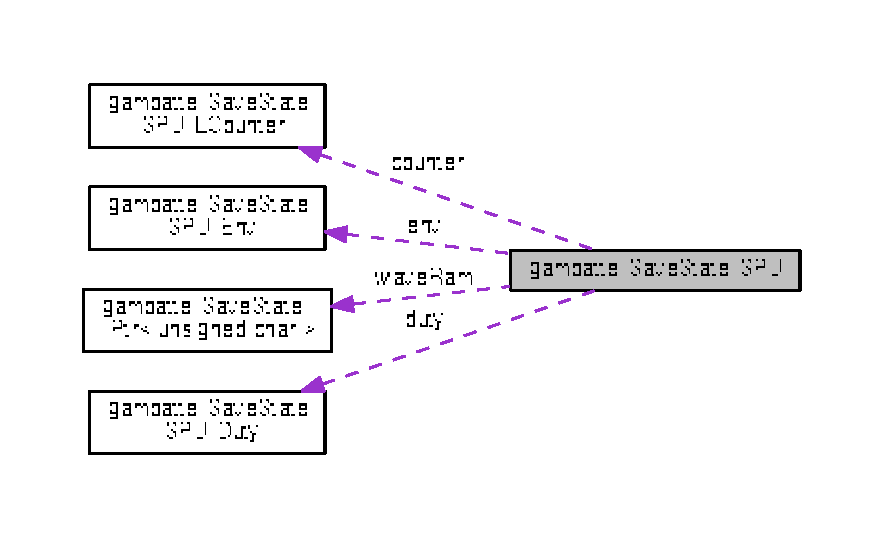
\includegraphics[width=350pt]{structgambatte_1_1SaveState_1_1SPU__coll__graph}
\end{center}
\end{figure}
\subsection*{Classes}
\begin{DoxyCompactItemize}
\item 
struct \hyperlink{structgambatte_1_1SaveState_1_1SPU_1_1Duty}{Duty}
\item 
struct \hyperlink{structgambatte_1_1SaveState_1_1SPU_1_1Env}{Env}
\item 
struct \hyperlink{structgambatte_1_1SaveState_1_1SPU_1_1LCounter}{L\+Counter}
\end{DoxyCompactItemize}
\subsection*{Public Attributes}
\begin{DoxyCompactItemize}
\item 
\begin{tabbing}
xx\=xx\=xx\=xx\=xx\=xx\=xx\=xx\=xx\=\kill
struct \{\\
\>struct \{\\
\>\>unsigned \hyperlink{structgambatte_1_1SaveState_1_1SPU_aa950836b4cdeb642d7c2891826536b5d}{counter}\\
\>\>unsigned short \hyperlink{structgambatte_1_1SaveState_1_1SPU_a433a72dbe39b9fc3f2fd084804fde0aa}{shadow}\\
\>\>unsigned char \hyperlink{structgambatte_1_1SaveState_1_1SPU_a73a2fd5723e5c00954c0f13acc952655}{nr0}\\
\>\>bool \hyperlink{structgambatte_1_1SaveState_1_1SPU_a4d640d9fc422078a2bf196a3981976d5}{negging}\\
\>\} \hyperlink{structgambatte_1_1SaveState_1_1SPU_abc7d3976ddfd29cb74c101499cc938e7}{sweep}\\
\>\hyperlink{structgambatte_1_1SaveState_1_1SPU_1_1Duty}{Duty} \hyperlink{structgambatte_1_1SaveState_1_1SPU_af246d67bf639590df08beff9255a610b}{duty}\\
\>\hyperlink{structgambatte_1_1SaveState_1_1SPU_1_1Env}{Env} \hyperlink{structgambatte_1_1SaveState_1_1SPU_a39d86c1ace4a0e800fe73910a887ef24}{env}\\
\>\hyperlink{structgambatte_1_1SaveState_1_1SPU_1_1LCounter}{LCounter} \hyperlink{structgambatte_1_1SaveState_1_1SPU_ab0e4f21b99cff7f36a59855ecb00cbb1}{lcounter}\\
\>unsigned char \hyperlink{structgambatte_1_1SaveState_1_1SPU_a9395abdc0d09126fac7ca2edfeda9701}{nr4}\\
\>bool \hyperlink{structgambatte_1_1SaveState_1_1SPU_affe87b653ce5fc88a9cf550ad83d9437}{master}\\
\} \hyperlink{structgambatte_1_1SaveState_1_1SPU_a0249d80be054e4094494b63f5432b31f}{ch1}\\

\end{tabbing}\item 
\begin{tabbing}
xx\=xx\=xx\=xx\=xx\=xx\=xx\=xx\=xx\=\kill
struct \{\\
\>\hyperlink{structgambatte_1_1SaveState_1_1SPU_1_1Duty}{Duty} \hyperlink{structgambatte_1_1SaveState_1_1SPU_af246d67bf639590df08beff9255a610b}{duty}\\
\>\hyperlink{structgambatte_1_1SaveState_1_1SPU_1_1Env}{Env} \hyperlink{structgambatte_1_1SaveState_1_1SPU_a39d86c1ace4a0e800fe73910a887ef24}{env}\\
\>\hyperlink{structgambatte_1_1SaveState_1_1SPU_1_1LCounter}{LCounter} \hyperlink{structgambatte_1_1SaveState_1_1SPU_ab0e4f21b99cff7f36a59855ecb00cbb1}{lcounter}\\
\>unsigned char \hyperlink{structgambatte_1_1SaveState_1_1SPU_a9395abdc0d09126fac7ca2edfeda9701}{nr4}\\
\>bool \hyperlink{structgambatte_1_1SaveState_1_1SPU_affe87b653ce5fc88a9cf550ad83d9437}{master}\\
\} \hyperlink{structgambatte_1_1SaveState_1_1SPU_a72e47a898d372e129589e59e4a1ec044}{ch2}\\

\end{tabbing}\item 
\begin{tabbing}
xx\=xx\=xx\=xx\=xx\=xx\=xx\=xx\=xx\=\kill
struct \{\\
\>\hyperlink{classgambatte_1_1SaveState_1_1Ptr}{Ptr}$<$ unsigned char $>$ \hyperlink{structgambatte_1_1SaveState_1_1SPU_af385ccd5872ee4a92752e9017b797402}{waveRam}\\
\>\hyperlink{structgambatte_1_1SaveState_1_1SPU_1_1LCounter}{LCounter} \hyperlink{structgambatte_1_1SaveState_1_1SPU_ab0e4f21b99cff7f36a59855ecb00cbb1}{lcounter}\\
\>unsigned \hyperlink{structgambatte_1_1SaveState_1_1SPU_abd17b3a40b40b19f716f695d88ef1f16}{waveCounter}\\
\>unsigned \hyperlink{structgambatte_1_1SaveState_1_1SPU_af0a8956e43b491799783309dc9cf26b4}{lastReadTime}\\
\>unsigned char \hyperlink{structgambatte_1_1SaveState_1_1SPU_a69e97d400e51c6c64ab0a1d0e0f714e5}{nr3}\\
\>unsigned char \hyperlink{structgambatte_1_1SaveState_1_1SPU_a9395abdc0d09126fac7ca2edfeda9701}{nr4}\\
\>unsigned char \hyperlink{structgambatte_1_1SaveState_1_1SPU_a34262510738618c8969cf29fa20808f2}{wavePos}\\
\>unsigned char \hyperlink{structgambatte_1_1SaveState_1_1SPU_ae66c5dc91fd2a1c4addd10fe2e86d30a}{sampleBuf}\\
\>bool \hyperlink{structgambatte_1_1SaveState_1_1SPU_affe87b653ce5fc88a9cf550ad83d9437}{master}\\
\} \hyperlink{structgambatte_1_1SaveState_1_1SPU_a106741ea3e1769480b7cf2aa3652e57b}{ch3}\\

\end{tabbing}\item 
\begin{tabbing}
xx\=xx\=xx\=xx\=xx\=xx\=xx\=xx\=xx\=\kill
struct \{\\
\>struct \{\\
\>\>unsigned \hyperlink{structgambatte_1_1SaveState_1_1SPU_aa950836b4cdeb642d7c2891826536b5d}{counter}\\
\>\>unsigned short \hyperlink{structgambatte_1_1SaveState_1_1SPU_a7d30f12abc09b3f8c6f4b88f63ad7265}{reg}\\
\>\} \hyperlink{structgambatte_1_1SaveState_1_1SPU_a53d6590772c1fa24ec428c00211279dd}{lfsr}\\
\>\hyperlink{structgambatte_1_1SaveState_1_1SPU_1_1Env}{Env} \hyperlink{structgambatte_1_1SaveState_1_1SPU_a39d86c1ace4a0e800fe73910a887ef24}{env}\\
\>\hyperlink{structgambatte_1_1SaveState_1_1SPU_1_1LCounter}{LCounter} \hyperlink{structgambatte_1_1SaveState_1_1SPU_ab0e4f21b99cff7f36a59855ecb00cbb1}{lcounter}\\
\>unsigned char \hyperlink{structgambatte_1_1SaveState_1_1SPU_a9395abdc0d09126fac7ca2edfeda9701}{nr4}\\
\>bool \hyperlink{structgambatte_1_1SaveState_1_1SPU_affe87b653ce5fc88a9cf550ad83d9437}{master}\\
\} \hyperlink{structgambatte_1_1SaveState_1_1SPU_a0faab2840aec3741d2229e44d3963c93}{ch4}\\

\end{tabbing}\item 
unsigned \hyperlink{structgambatte_1_1SaveState_1_1SPU_a2560277764c98a6796fe77250b24e9f7}{cycle\+Counter}
\end{DoxyCompactItemize}


\subsection{Member Data Documentation}
\mbox{\Hypertarget{structgambatte_1_1SaveState_1_1SPU_a0249d80be054e4094494b63f5432b31f}\label{structgambatte_1_1SaveState_1_1SPU_a0249d80be054e4094494b63f5432b31f}} 
\index{gambatte\+::\+Save\+State\+::\+S\+PU@{gambatte\+::\+Save\+State\+::\+S\+PU}!ch1@{ch1}}
\index{ch1@{ch1}!gambatte\+::\+Save\+State\+::\+S\+PU@{gambatte\+::\+Save\+State\+::\+S\+PU}}
\subsubsection{\texorpdfstring{ch1}{ch1}}
{\footnotesize\ttfamily struct \{ ... \}   gambatte\+::\+Save\+State\+::\+S\+P\+U\+::ch1}

\mbox{\Hypertarget{structgambatte_1_1SaveState_1_1SPU_a72e47a898d372e129589e59e4a1ec044}\label{structgambatte_1_1SaveState_1_1SPU_a72e47a898d372e129589e59e4a1ec044}} 
\index{gambatte\+::\+Save\+State\+::\+S\+PU@{gambatte\+::\+Save\+State\+::\+S\+PU}!ch2@{ch2}}
\index{ch2@{ch2}!gambatte\+::\+Save\+State\+::\+S\+PU@{gambatte\+::\+Save\+State\+::\+S\+PU}}
\subsubsection{\texorpdfstring{ch2}{ch2}}
{\footnotesize\ttfamily struct \{ ... \}   gambatte\+::\+Save\+State\+::\+S\+P\+U\+::ch2}

\mbox{\Hypertarget{structgambatte_1_1SaveState_1_1SPU_a106741ea3e1769480b7cf2aa3652e57b}\label{structgambatte_1_1SaveState_1_1SPU_a106741ea3e1769480b7cf2aa3652e57b}} 
\index{gambatte\+::\+Save\+State\+::\+S\+PU@{gambatte\+::\+Save\+State\+::\+S\+PU}!ch3@{ch3}}
\index{ch3@{ch3}!gambatte\+::\+Save\+State\+::\+S\+PU@{gambatte\+::\+Save\+State\+::\+S\+PU}}
\subsubsection{\texorpdfstring{ch3}{ch3}}
{\footnotesize\ttfamily struct \{ ... \}   gambatte\+::\+Save\+State\+::\+S\+P\+U\+::ch3}

\mbox{\Hypertarget{structgambatte_1_1SaveState_1_1SPU_a0faab2840aec3741d2229e44d3963c93}\label{structgambatte_1_1SaveState_1_1SPU_a0faab2840aec3741d2229e44d3963c93}} 
\index{gambatte\+::\+Save\+State\+::\+S\+PU@{gambatte\+::\+Save\+State\+::\+S\+PU}!ch4@{ch4}}
\index{ch4@{ch4}!gambatte\+::\+Save\+State\+::\+S\+PU@{gambatte\+::\+Save\+State\+::\+S\+PU}}
\subsubsection{\texorpdfstring{ch4}{ch4}}
{\footnotesize\ttfamily struct \{ ... \}   gambatte\+::\+Save\+State\+::\+S\+P\+U\+::ch4}

\mbox{\Hypertarget{structgambatte_1_1SaveState_1_1SPU_aa950836b4cdeb642d7c2891826536b5d}\label{structgambatte_1_1SaveState_1_1SPU_aa950836b4cdeb642d7c2891826536b5d}} 
\index{gambatte\+::\+Save\+State\+::\+S\+PU@{gambatte\+::\+Save\+State\+::\+S\+PU}!counter@{counter}}
\index{counter@{counter}!gambatte\+::\+Save\+State\+::\+S\+PU@{gambatte\+::\+Save\+State\+::\+S\+PU}}
\subsubsection{\texorpdfstring{counter}{counter}}
{\footnotesize\ttfamily unsigned gambatte\+::\+Save\+State\+::\+S\+P\+U\+::counter}

\mbox{\Hypertarget{structgambatte_1_1SaveState_1_1SPU_a2560277764c98a6796fe77250b24e9f7}\label{structgambatte_1_1SaveState_1_1SPU_a2560277764c98a6796fe77250b24e9f7}} 
\index{gambatte\+::\+Save\+State\+::\+S\+PU@{gambatte\+::\+Save\+State\+::\+S\+PU}!cycle\+Counter@{cycle\+Counter}}
\index{cycle\+Counter@{cycle\+Counter}!gambatte\+::\+Save\+State\+::\+S\+PU@{gambatte\+::\+Save\+State\+::\+S\+PU}}
\subsubsection{\texorpdfstring{cycle\+Counter}{cycleCounter}}
{\footnotesize\ttfamily unsigned gambatte\+::\+Save\+State\+::\+S\+P\+U\+::cycle\+Counter}

\mbox{\Hypertarget{structgambatte_1_1SaveState_1_1SPU_af246d67bf639590df08beff9255a610b}\label{structgambatte_1_1SaveState_1_1SPU_af246d67bf639590df08beff9255a610b}} 
\index{gambatte\+::\+Save\+State\+::\+S\+PU@{gambatte\+::\+Save\+State\+::\+S\+PU}!duty@{duty}}
\index{duty@{duty}!gambatte\+::\+Save\+State\+::\+S\+PU@{gambatte\+::\+Save\+State\+::\+S\+PU}}
\subsubsection{\texorpdfstring{duty}{duty}}
{\footnotesize\ttfamily \hyperlink{structgambatte_1_1SaveState_1_1SPU_1_1Duty}{Duty} gambatte\+::\+Save\+State\+::\+S\+P\+U\+::duty}

\mbox{\Hypertarget{structgambatte_1_1SaveState_1_1SPU_a39d86c1ace4a0e800fe73910a887ef24}\label{structgambatte_1_1SaveState_1_1SPU_a39d86c1ace4a0e800fe73910a887ef24}} 
\index{gambatte\+::\+Save\+State\+::\+S\+PU@{gambatte\+::\+Save\+State\+::\+S\+PU}!env@{env}}
\index{env@{env}!gambatte\+::\+Save\+State\+::\+S\+PU@{gambatte\+::\+Save\+State\+::\+S\+PU}}
\subsubsection{\texorpdfstring{env}{env}}
{\footnotesize\ttfamily \hyperlink{structgambatte_1_1SaveState_1_1SPU_1_1Env}{Env} gambatte\+::\+Save\+State\+::\+S\+P\+U\+::env}

\mbox{\Hypertarget{structgambatte_1_1SaveState_1_1SPU_af0a8956e43b491799783309dc9cf26b4}\label{structgambatte_1_1SaveState_1_1SPU_af0a8956e43b491799783309dc9cf26b4}} 
\index{gambatte\+::\+Save\+State\+::\+S\+PU@{gambatte\+::\+Save\+State\+::\+S\+PU}!last\+Read\+Time@{last\+Read\+Time}}
\index{last\+Read\+Time@{last\+Read\+Time}!gambatte\+::\+Save\+State\+::\+S\+PU@{gambatte\+::\+Save\+State\+::\+S\+PU}}
\subsubsection{\texorpdfstring{last\+Read\+Time}{lastReadTime}}
{\footnotesize\ttfamily unsigned gambatte\+::\+Save\+State\+::\+S\+P\+U\+::last\+Read\+Time}

\mbox{\Hypertarget{structgambatte_1_1SaveState_1_1SPU_ab0e4f21b99cff7f36a59855ecb00cbb1}\label{structgambatte_1_1SaveState_1_1SPU_ab0e4f21b99cff7f36a59855ecb00cbb1}} 
\index{gambatte\+::\+Save\+State\+::\+S\+PU@{gambatte\+::\+Save\+State\+::\+S\+PU}!lcounter@{lcounter}}
\index{lcounter@{lcounter}!gambatte\+::\+Save\+State\+::\+S\+PU@{gambatte\+::\+Save\+State\+::\+S\+PU}}
\subsubsection{\texorpdfstring{lcounter}{lcounter}}
{\footnotesize\ttfamily \hyperlink{structgambatte_1_1SaveState_1_1SPU_1_1LCounter}{L\+Counter} gambatte\+::\+Save\+State\+::\+S\+P\+U\+::lcounter}

\mbox{\Hypertarget{structgambatte_1_1SaveState_1_1SPU_a53d6590772c1fa24ec428c00211279dd}\label{structgambatte_1_1SaveState_1_1SPU_a53d6590772c1fa24ec428c00211279dd}} 
\index{gambatte\+::\+Save\+State\+::\+S\+PU@{gambatte\+::\+Save\+State\+::\+S\+PU}!lfsr@{lfsr}}
\index{lfsr@{lfsr}!gambatte\+::\+Save\+State\+::\+S\+PU@{gambatte\+::\+Save\+State\+::\+S\+PU}}
\subsubsection{\texorpdfstring{lfsr}{lfsr}}
{\footnotesize\ttfamily struct \{ ... \}   gambatte\+::\+Save\+State\+::\+S\+P\+U\+::lfsr}

\mbox{\Hypertarget{structgambatte_1_1SaveState_1_1SPU_affe87b653ce5fc88a9cf550ad83d9437}\label{structgambatte_1_1SaveState_1_1SPU_affe87b653ce5fc88a9cf550ad83d9437}} 
\index{gambatte\+::\+Save\+State\+::\+S\+PU@{gambatte\+::\+Save\+State\+::\+S\+PU}!master@{master}}
\index{master@{master}!gambatte\+::\+Save\+State\+::\+S\+PU@{gambatte\+::\+Save\+State\+::\+S\+PU}}
\subsubsection{\texorpdfstring{master}{master}}
{\footnotesize\ttfamily bool gambatte\+::\+Save\+State\+::\+S\+P\+U\+::master}

\mbox{\Hypertarget{structgambatte_1_1SaveState_1_1SPU_a4d640d9fc422078a2bf196a3981976d5}\label{structgambatte_1_1SaveState_1_1SPU_a4d640d9fc422078a2bf196a3981976d5}} 
\index{gambatte\+::\+Save\+State\+::\+S\+PU@{gambatte\+::\+Save\+State\+::\+S\+PU}!negging@{negging}}
\index{negging@{negging}!gambatte\+::\+Save\+State\+::\+S\+PU@{gambatte\+::\+Save\+State\+::\+S\+PU}}
\subsubsection{\texorpdfstring{negging}{negging}}
{\footnotesize\ttfamily bool gambatte\+::\+Save\+State\+::\+S\+P\+U\+::negging}

\mbox{\Hypertarget{structgambatte_1_1SaveState_1_1SPU_a73a2fd5723e5c00954c0f13acc952655}\label{structgambatte_1_1SaveState_1_1SPU_a73a2fd5723e5c00954c0f13acc952655}} 
\index{gambatte\+::\+Save\+State\+::\+S\+PU@{gambatte\+::\+Save\+State\+::\+S\+PU}!nr0@{nr0}}
\index{nr0@{nr0}!gambatte\+::\+Save\+State\+::\+S\+PU@{gambatte\+::\+Save\+State\+::\+S\+PU}}
\subsubsection{\texorpdfstring{nr0}{nr0}}
{\footnotesize\ttfamily unsigned char gambatte\+::\+Save\+State\+::\+S\+P\+U\+::nr0}

\mbox{\Hypertarget{structgambatte_1_1SaveState_1_1SPU_a69e97d400e51c6c64ab0a1d0e0f714e5}\label{structgambatte_1_1SaveState_1_1SPU_a69e97d400e51c6c64ab0a1d0e0f714e5}} 
\index{gambatte\+::\+Save\+State\+::\+S\+PU@{gambatte\+::\+Save\+State\+::\+S\+PU}!nr3@{nr3}}
\index{nr3@{nr3}!gambatte\+::\+Save\+State\+::\+S\+PU@{gambatte\+::\+Save\+State\+::\+S\+PU}}
\subsubsection{\texorpdfstring{nr3}{nr3}}
{\footnotesize\ttfamily unsigned char gambatte\+::\+Save\+State\+::\+S\+P\+U\+::nr3}

\mbox{\Hypertarget{structgambatte_1_1SaveState_1_1SPU_a9395abdc0d09126fac7ca2edfeda9701}\label{structgambatte_1_1SaveState_1_1SPU_a9395abdc0d09126fac7ca2edfeda9701}} 
\index{gambatte\+::\+Save\+State\+::\+S\+PU@{gambatte\+::\+Save\+State\+::\+S\+PU}!nr4@{nr4}}
\index{nr4@{nr4}!gambatte\+::\+Save\+State\+::\+S\+PU@{gambatte\+::\+Save\+State\+::\+S\+PU}}
\subsubsection{\texorpdfstring{nr4}{nr4}}
{\footnotesize\ttfamily unsigned char gambatte\+::\+Save\+State\+::\+S\+P\+U\+::nr4}

\mbox{\Hypertarget{structgambatte_1_1SaveState_1_1SPU_a7d30f12abc09b3f8c6f4b88f63ad7265}\label{structgambatte_1_1SaveState_1_1SPU_a7d30f12abc09b3f8c6f4b88f63ad7265}} 
\index{gambatte\+::\+Save\+State\+::\+S\+PU@{gambatte\+::\+Save\+State\+::\+S\+PU}!reg@{reg}}
\index{reg@{reg}!gambatte\+::\+Save\+State\+::\+S\+PU@{gambatte\+::\+Save\+State\+::\+S\+PU}}
\subsubsection{\texorpdfstring{reg}{reg}}
{\footnotesize\ttfamily unsigned short gambatte\+::\+Save\+State\+::\+S\+P\+U\+::reg}

\mbox{\Hypertarget{structgambatte_1_1SaveState_1_1SPU_ae66c5dc91fd2a1c4addd10fe2e86d30a}\label{structgambatte_1_1SaveState_1_1SPU_ae66c5dc91fd2a1c4addd10fe2e86d30a}} 
\index{gambatte\+::\+Save\+State\+::\+S\+PU@{gambatte\+::\+Save\+State\+::\+S\+PU}!sample\+Buf@{sample\+Buf}}
\index{sample\+Buf@{sample\+Buf}!gambatte\+::\+Save\+State\+::\+S\+PU@{gambatte\+::\+Save\+State\+::\+S\+PU}}
\subsubsection{\texorpdfstring{sample\+Buf}{sampleBuf}}
{\footnotesize\ttfamily unsigned char gambatte\+::\+Save\+State\+::\+S\+P\+U\+::sample\+Buf}

\mbox{\Hypertarget{structgambatte_1_1SaveState_1_1SPU_a433a72dbe39b9fc3f2fd084804fde0aa}\label{structgambatte_1_1SaveState_1_1SPU_a433a72dbe39b9fc3f2fd084804fde0aa}} 
\index{gambatte\+::\+Save\+State\+::\+S\+PU@{gambatte\+::\+Save\+State\+::\+S\+PU}!shadow@{shadow}}
\index{shadow@{shadow}!gambatte\+::\+Save\+State\+::\+S\+PU@{gambatte\+::\+Save\+State\+::\+S\+PU}}
\subsubsection{\texorpdfstring{shadow}{shadow}}
{\footnotesize\ttfamily unsigned short gambatte\+::\+Save\+State\+::\+S\+P\+U\+::shadow}

\mbox{\Hypertarget{structgambatte_1_1SaveState_1_1SPU_abc7d3976ddfd29cb74c101499cc938e7}\label{structgambatte_1_1SaveState_1_1SPU_abc7d3976ddfd29cb74c101499cc938e7}} 
\index{gambatte\+::\+Save\+State\+::\+S\+PU@{gambatte\+::\+Save\+State\+::\+S\+PU}!sweep@{sweep}}
\index{sweep@{sweep}!gambatte\+::\+Save\+State\+::\+S\+PU@{gambatte\+::\+Save\+State\+::\+S\+PU}}
\subsubsection{\texorpdfstring{sweep}{sweep}}
{\footnotesize\ttfamily struct \{ ... \}   gambatte\+::\+Save\+State\+::\+S\+P\+U\+::sweep}

\mbox{\Hypertarget{structgambatte_1_1SaveState_1_1SPU_abd17b3a40b40b19f716f695d88ef1f16}\label{structgambatte_1_1SaveState_1_1SPU_abd17b3a40b40b19f716f695d88ef1f16}} 
\index{gambatte\+::\+Save\+State\+::\+S\+PU@{gambatte\+::\+Save\+State\+::\+S\+PU}!wave\+Counter@{wave\+Counter}}
\index{wave\+Counter@{wave\+Counter}!gambatte\+::\+Save\+State\+::\+S\+PU@{gambatte\+::\+Save\+State\+::\+S\+PU}}
\subsubsection{\texorpdfstring{wave\+Counter}{waveCounter}}
{\footnotesize\ttfamily unsigned gambatte\+::\+Save\+State\+::\+S\+P\+U\+::wave\+Counter}

\mbox{\Hypertarget{structgambatte_1_1SaveState_1_1SPU_a34262510738618c8969cf29fa20808f2}\label{structgambatte_1_1SaveState_1_1SPU_a34262510738618c8969cf29fa20808f2}} 
\index{gambatte\+::\+Save\+State\+::\+S\+PU@{gambatte\+::\+Save\+State\+::\+S\+PU}!wave\+Pos@{wave\+Pos}}
\index{wave\+Pos@{wave\+Pos}!gambatte\+::\+Save\+State\+::\+S\+PU@{gambatte\+::\+Save\+State\+::\+S\+PU}}
\subsubsection{\texorpdfstring{wave\+Pos}{wavePos}}
{\footnotesize\ttfamily unsigned char gambatte\+::\+Save\+State\+::\+S\+P\+U\+::wave\+Pos}

\mbox{\Hypertarget{structgambatte_1_1SaveState_1_1SPU_af385ccd5872ee4a92752e9017b797402}\label{structgambatte_1_1SaveState_1_1SPU_af385ccd5872ee4a92752e9017b797402}} 
\index{gambatte\+::\+Save\+State\+::\+S\+PU@{gambatte\+::\+Save\+State\+::\+S\+PU}!wave\+Ram@{wave\+Ram}}
\index{wave\+Ram@{wave\+Ram}!gambatte\+::\+Save\+State\+::\+S\+PU@{gambatte\+::\+Save\+State\+::\+S\+PU}}
\subsubsection{\texorpdfstring{wave\+Ram}{waveRam}}
{\footnotesize\ttfamily \hyperlink{classgambatte_1_1SaveState_1_1Ptr}{Ptr}$<$unsigned char$>$ gambatte\+::\+Save\+State\+::\+S\+P\+U\+::wave\+Ram}



The documentation for this struct was generated from the following file\+:\begin{DoxyCompactItemize}
\item 
src/\hyperlink{savestate_8h}{savestate.\+h}\end{DoxyCompactItemize}

\hypertarget{classgambatte_1_1StateSaver}{}\section{gambatte\+:\+:State\+Saver Class Reference}
\label{classgambatte_1_1StateSaver}\index{gambatte\+::\+State\+Saver@{gambatte\+::\+State\+Saver}}


{\ttfamily \#include $<$statesaver.\+h$>$}

\subsection*{Public Types}
\begin{DoxyCompactItemize}
\item 
enum \{ \hyperlink{classgambatte_1_1StateSaver_ae198109f1afd0eeae59a056efb659a62a796008c573f248ed2df587a64bd2c56a}{ss\+\_\+shift} = 2
 \}
\item 
enum \{ \hyperlink{classgambatte_1_1StateSaver_a7a727a444a7f39b775b6fa00a4d8b7b7a57157847503e09dbb1b5c83a7fe98ace}{ss\+\_\+div} = 1 $<$$<$ 2
 \}
\item 
enum \{ \hyperlink{classgambatte_1_1StateSaver_a37f3c4400dc9ae31ee260a16dc580a63ac4459ac125ae22c280a7bb1b45b0878a}{ss\+\_\+width} = 160 $>$$>$ ss\+\_\+shift
 \}
\item 
enum \{ \hyperlink{classgambatte_1_1StateSaver_a46feccb5e5ac95e30777dd3442559095a850759c51b83eb9eeb127cd21d3ca232}{ss\+\_\+height} = 144 $>$$>$ ss\+\_\+shift
 \}
\end{DoxyCompactItemize}
\subsection*{Static Public Member Functions}
\begin{DoxyCompactItemize}
\item 
static bool \hyperlink{classgambatte_1_1StateSaver_abbc44cde3c1406a300656c57574453e8}{save\+State} (\hyperlink{structgambatte_1_1SaveState}{Save\+State} const \&\hyperlink{ppu_8cpp_a2f2eca6997ee7baf8901725ae074d45b}{state}, \hyperlink{namespacegambatte_a0639f09fccfbbd5a8e0796318768e370}{uint\+\_\+least32\+\_\+t} const $\ast$video\+Buf, std\+::ptrdiff\+\_\+t pitch, std\+::string const \&\hyperlink{ioapi_8h_a7a03a664b090ce5c848ecb31cb4a2fa8}{filename})
\item 
static bool \hyperlink{classgambatte_1_1StateSaver_a0abf1c65ad9d738043fcc8ef819d4bef}{load\+State} (\hyperlink{structgambatte_1_1SaveState}{Save\+State} \&\hyperlink{ppu_8cpp_a2f2eca6997ee7baf8901725ae074d45b}{state}, std\+::string const \&\hyperlink{ioapi_8h_a7a03a664b090ce5c848ecb31cb4a2fa8}{filename})
\end{DoxyCompactItemize}
\subsection*{Private Member Functions}
\begin{DoxyCompactItemize}
\item 
\hyperlink{classgambatte_1_1StateSaver_a90d9649f1f12948209b6b7b00567b765}{State\+Saver} ()
\end{DoxyCompactItemize}


\subsection{Member Enumeration Documentation}
\mbox{\Hypertarget{classgambatte_1_1StateSaver_ae198109f1afd0eeae59a056efb659a62}\label{classgambatte_1_1StateSaver_ae198109f1afd0eeae59a056efb659a62}} 
\subsubsection{\texorpdfstring{anonymous enum}{anonymous enum}}
{\footnotesize\ttfamily anonymous enum}

\begin{DoxyEnumFields}{Enumerator}
\raisebox{\heightof{T}}[0pt][0pt]{\index{ss\+\_\+shift@{ss\+\_\+shift}!gambatte\+::\+State\+Saver@{gambatte\+::\+State\+Saver}}\index{gambatte\+::\+State\+Saver@{gambatte\+::\+State\+Saver}!ss\+\_\+shift@{ss\+\_\+shift}}}\mbox{\Hypertarget{classgambatte_1_1StateSaver_ae198109f1afd0eeae59a056efb659a62a796008c573f248ed2df587a64bd2c56a}\label{classgambatte_1_1StateSaver_ae198109f1afd0eeae59a056efb659a62a796008c573f248ed2df587a64bd2c56a}} 
ss\+\_\+shift&\\
\hline

\end{DoxyEnumFields}
\mbox{\Hypertarget{classgambatte_1_1StateSaver_a7a727a444a7f39b775b6fa00a4d8b7b7}\label{classgambatte_1_1StateSaver_a7a727a444a7f39b775b6fa00a4d8b7b7}} 
\subsubsection{\texorpdfstring{anonymous enum}{anonymous enum}}
{\footnotesize\ttfamily anonymous enum}

\begin{DoxyEnumFields}{Enumerator}
\raisebox{\heightof{T}}[0pt][0pt]{\index{ss\+\_\+div@{ss\+\_\+div}!gambatte\+::\+State\+Saver@{gambatte\+::\+State\+Saver}}\index{gambatte\+::\+State\+Saver@{gambatte\+::\+State\+Saver}!ss\+\_\+div@{ss\+\_\+div}}}\mbox{\Hypertarget{classgambatte_1_1StateSaver_a7a727a444a7f39b775b6fa00a4d8b7b7a57157847503e09dbb1b5c83a7fe98ace}\label{classgambatte_1_1StateSaver_a7a727a444a7f39b775b6fa00a4d8b7b7a57157847503e09dbb1b5c83a7fe98ace}} 
ss\+\_\+div&\\
\hline

\end{DoxyEnumFields}
\mbox{\Hypertarget{classgambatte_1_1StateSaver_a37f3c4400dc9ae31ee260a16dc580a63}\label{classgambatte_1_1StateSaver_a37f3c4400dc9ae31ee260a16dc580a63}} 
\subsubsection{\texorpdfstring{anonymous enum}{anonymous enum}}
{\footnotesize\ttfamily anonymous enum}

\begin{DoxyEnumFields}{Enumerator}
\raisebox{\heightof{T}}[0pt][0pt]{\index{ss\+\_\+width@{ss\+\_\+width}!gambatte\+::\+State\+Saver@{gambatte\+::\+State\+Saver}}\index{gambatte\+::\+State\+Saver@{gambatte\+::\+State\+Saver}!ss\+\_\+width@{ss\+\_\+width}}}\mbox{\Hypertarget{classgambatte_1_1StateSaver_a37f3c4400dc9ae31ee260a16dc580a63ac4459ac125ae22c280a7bb1b45b0878a}\label{classgambatte_1_1StateSaver_a37f3c4400dc9ae31ee260a16dc580a63ac4459ac125ae22c280a7bb1b45b0878a}} 
ss\+\_\+width&\\
\hline

\end{DoxyEnumFields}
\mbox{\Hypertarget{classgambatte_1_1StateSaver_a46feccb5e5ac95e30777dd3442559095}\label{classgambatte_1_1StateSaver_a46feccb5e5ac95e30777dd3442559095}} 
\subsubsection{\texorpdfstring{anonymous enum}{anonymous enum}}
{\footnotesize\ttfamily anonymous enum}

\begin{DoxyEnumFields}{Enumerator}
\raisebox{\heightof{T}}[0pt][0pt]{\index{ss\+\_\+height@{ss\+\_\+height}!gambatte\+::\+State\+Saver@{gambatte\+::\+State\+Saver}}\index{gambatte\+::\+State\+Saver@{gambatte\+::\+State\+Saver}!ss\+\_\+height@{ss\+\_\+height}}}\mbox{\Hypertarget{classgambatte_1_1StateSaver_a46feccb5e5ac95e30777dd3442559095a850759c51b83eb9eeb127cd21d3ca232}\label{classgambatte_1_1StateSaver_a46feccb5e5ac95e30777dd3442559095a850759c51b83eb9eeb127cd21d3ca232}} 
ss\+\_\+height&\\
\hline

\end{DoxyEnumFields}


\subsection{Constructor \& Destructor Documentation}
\mbox{\Hypertarget{classgambatte_1_1StateSaver_a90d9649f1f12948209b6b7b00567b765}\label{classgambatte_1_1StateSaver_a90d9649f1f12948209b6b7b00567b765}} 
\index{gambatte\+::\+State\+Saver@{gambatte\+::\+State\+Saver}!State\+Saver@{State\+Saver}}
\index{State\+Saver@{State\+Saver}!gambatte\+::\+State\+Saver@{gambatte\+::\+State\+Saver}}
\subsubsection{\texorpdfstring{State\+Saver()}{StateSaver()}}
{\footnotesize\ttfamily gambatte\+::\+State\+Saver\+::\+State\+Saver (\begin{DoxyParamCaption}{ }\end{DoxyParamCaption})\hspace{0.3cm}{\ttfamily [private]}}



\subsection{Member Function Documentation}
\mbox{\Hypertarget{classgambatte_1_1StateSaver_a0abf1c65ad9d738043fcc8ef819d4bef}\label{classgambatte_1_1StateSaver_a0abf1c65ad9d738043fcc8ef819d4bef}} 
\index{gambatte\+::\+State\+Saver@{gambatte\+::\+State\+Saver}!load\+State@{load\+State}}
\index{load\+State@{load\+State}!gambatte\+::\+State\+Saver@{gambatte\+::\+State\+Saver}}
\subsubsection{\texorpdfstring{load\+State()}{loadState()}}
{\footnotesize\ttfamily bool gambatte\+::\+State\+Saver\+::load\+State (\begin{DoxyParamCaption}\item[{\hyperlink{structgambatte_1_1SaveState}{Save\+State} \&}]{state,  }\item[{std\+::string const \&}]{filename }\end{DoxyParamCaption})\hspace{0.3cm}{\ttfamily [static]}}

\mbox{\Hypertarget{classgambatte_1_1StateSaver_abbc44cde3c1406a300656c57574453e8}\label{classgambatte_1_1StateSaver_abbc44cde3c1406a300656c57574453e8}} 
\index{gambatte\+::\+State\+Saver@{gambatte\+::\+State\+Saver}!save\+State@{save\+State}}
\index{save\+State@{save\+State}!gambatte\+::\+State\+Saver@{gambatte\+::\+State\+Saver}}
\subsubsection{\texorpdfstring{save\+State()}{saveState()}}
{\footnotesize\ttfamily bool gambatte\+::\+State\+Saver\+::save\+State (\begin{DoxyParamCaption}\item[{\hyperlink{structgambatte_1_1SaveState}{Save\+State} const \&}]{state,  }\item[{\hyperlink{namespacegambatte_a0639f09fccfbbd5a8e0796318768e370}{uint\+\_\+least32\+\_\+t} const $\ast$}]{video\+Buf,  }\item[{std\+::ptrdiff\+\_\+t}]{pitch,  }\item[{std\+::string const \&}]{filename }\end{DoxyParamCaption})\hspace{0.3cm}{\ttfamily [static]}}



The documentation for this class was generated from the following files\+:\begin{DoxyCompactItemize}
\item 
src/\hyperlink{statesaver_8h}{statesaver.\+h}\item 
src/\hyperlink{statesaver_8cpp}{statesaver.\+cpp}\end{DoxyCompactItemize}

\hypertarget{classgambatte_1_1StaticOutputTester}{}\section{gambatte\+:\+:Static\+Output\+Tester$<$ Channel, Unit $>$ Class Template Reference}
\label{classgambatte_1_1StaticOutputTester}\index{gambatte\+::\+Static\+Output\+Tester$<$ Channel, Unit $>$@{gambatte\+::\+Static\+Output\+Tester$<$ Channel, Unit $>$}}


{\ttfamily \#include $<$static\+\_\+output\+\_\+tester.\+h$>$}



Inheritance diagram for gambatte\+:\+:Static\+Output\+Tester$<$ Channel, Unit $>$\+:\nopagebreak
\begin{figure}[H]
\begin{center}
\leavevmode
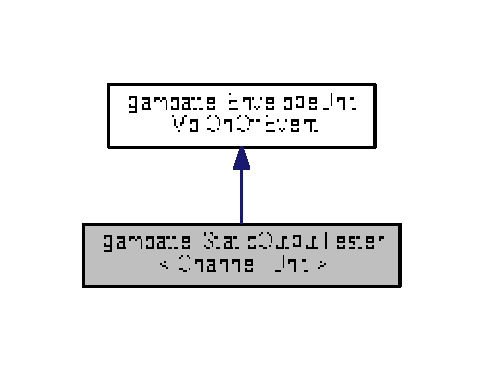
\includegraphics[width=232pt]{classgambatte_1_1StaticOutputTester__inherit__graph}
\end{center}
\end{figure}


Collaboration diagram for gambatte\+:\+:Static\+Output\+Tester$<$ Channel, Unit $>$\+:
\nopagebreak
\begin{figure}[H]
\begin{center}
\leavevmode
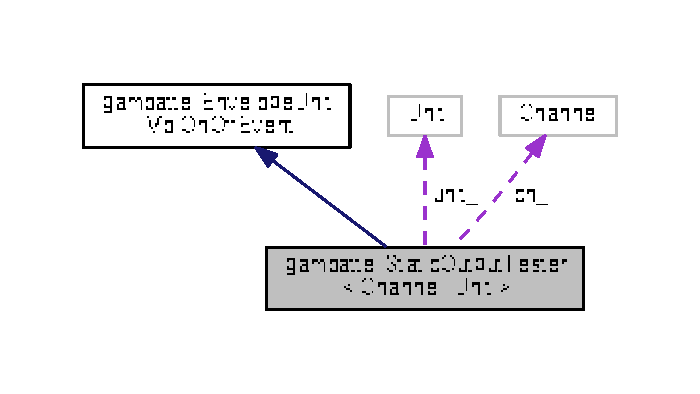
\includegraphics[width=336pt]{classgambatte_1_1StaticOutputTester__coll__graph}
\end{center}
\end{figure}
\subsection*{Public Member Functions}
\begin{DoxyCompactItemize}
\item 
\hyperlink{classgambatte_1_1StaticOutputTester_a598aaf698216da66440ebc9922cc3b77}{Static\+Output\+Tester} (Channel const \&ch, Unit \&unit)
\item 
void \hyperlink{classgambatte_1_1StaticOutputTester_a133c2bb69dd470d954954d4518dcdd4c}{operator()} (unsigned cc)
\end{DoxyCompactItemize}
\subsection*{Private Attributes}
\begin{DoxyCompactItemize}
\item 
Channel const  \& \hyperlink{classgambatte_1_1StaticOutputTester_a8c8666e9c317a775779c40bc2f7dda5d}{ch\+\_\+}
\item 
Unit \& \hyperlink{classgambatte_1_1StaticOutputTester_a23bbc293070a93e9b1d1071590ffb936}{unit\+\_\+}
\end{DoxyCompactItemize}


\subsection{Constructor \& Destructor Documentation}
\mbox{\Hypertarget{classgambatte_1_1StaticOutputTester_a598aaf698216da66440ebc9922cc3b77}\label{classgambatte_1_1StaticOutputTester_a598aaf698216da66440ebc9922cc3b77}} 
\index{gambatte\+::\+Static\+Output\+Tester@{gambatte\+::\+Static\+Output\+Tester}!Static\+Output\+Tester@{Static\+Output\+Tester}}
\index{Static\+Output\+Tester@{Static\+Output\+Tester}!gambatte\+::\+Static\+Output\+Tester@{gambatte\+::\+Static\+Output\+Tester}}
\subsubsection{\texorpdfstring{Static\+Output\+Tester()}{StaticOutputTester()}}
{\footnotesize\ttfamily template$<$class Channel, class Unit$>$ \\
\hyperlink{classgambatte_1_1StaticOutputTester}{gambatte\+::\+Static\+Output\+Tester}$<$ Channel, Unit $>$\+::\hyperlink{classgambatte_1_1StaticOutputTester}{Static\+Output\+Tester} (\begin{DoxyParamCaption}\item[{Channel const \&}]{ch,  }\item[{Unit \&}]{unit }\end{DoxyParamCaption})\hspace{0.3cm}{\ttfamily [inline]}}



\subsection{Member Function Documentation}
\mbox{\Hypertarget{classgambatte_1_1StaticOutputTester_a133c2bb69dd470d954954d4518dcdd4c}\label{classgambatte_1_1StaticOutputTester_a133c2bb69dd470d954954d4518dcdd4c}} 
\index{gambatte\+::\+Static\+Output\+Tester@{gambatte\+::\+Static\+Output\+Tester}!operator()@{operator()}}
\index{operator()@{operator()}!gambatte\+::\+Static\+Output\+Tester@{gambatte\+::\+Static\+Output\+Tester}}
\subsubsection{\texorpdfstring{operator()()}{operator()()}}
{\footnotesize\ttfamily template$<$class Channel , class Unit $>$ \\
void \hyperlink{classgambatte_1_1StaticOutputTester}{gambatte\+::\+Static\+Output\+Tester}$<$ Channel, Unit $>$\+::operator() (\begin{DoxyParamCaption}\item[{unsigned}]{cc }\end{DoxyParamCaption})\hspace{0.3cm}{\ttfamily [virtual]}}



Reimplemented from \hyperlink{structgambatte_1_1EnvelopeUnit_1_1VolOnOffEvent_a51a53f7c8e454be01a67e82a33dcf5ee}{gambatte\+::\+Envelope\+Unit\+::\+Vol\+On\+Off\+Event}.



\subsection{Member Data Documentation}
\mbox{\Hypertarget{classgambatte_1_1StaticOutputTester_a8c8666e9c317a775779c40bc2f7dda5d}\label{classgambatte_1_1StaticOutputTester_a8c8666e9c317a775779c40bc2f7dda5d}} 
\index{gambatte\+::\+Static\+Output\+Tester@{gambatte\+::\+Static\+Output\+Tester}!ch\+\_\+@{ch\+\_\+}}
\index{ch\+\_\+@{ch\+\_\+}!gambatte\+::\+Static\+Output\+Tester@{gambatte\+::\+Static\+Output\+Tester}}
\subsubsection{\texorpdfstring{ch\+\_\+}{ch\_}}
{\footnotesize\ttfamily template$<$class Channel, class Unit$>$ \\
Channel const\& \hyperlink{classgambatte_1_1StaticOutputTester}{gambatte\+::\+Static\+Output\+Tester}$<$ Channel, Unit $>$\+::ch\+\_\+\hspace{0.3cm}{\ttfamily [private]}}

\mbox{\Hypertarget{classgambatte_1_1StaticOutputTester_a23bbc293070a93e9b1d1071590ffb936}\label{classgambatte_1_1StaticOutputTester_a23bbc293070a93e9b1d1071590ffb936}} 
\index{gambatte\+::\+Static\+Output\+Tester@{gambatte\+::\+Static\+Output\+Tester}!unit\+\_\+@{unit\+\_\+}}
\index{unit\+\_\+@{unit\+\_\+}!gambatte\+::\+Static\+Output\+Tester@{gambatte\+::\+Static\+Output\+Tester}}
\subsubsection{\texorpdfstring{unit\+\_\+}{unit\_}}
{\footnotesize\ttfamily template$<$class Channel, class Unit$>$ \\
Unit\& \hyperlink{classgambatte_1_1StaticOutputTester}{gambatte\+::\+Static\+Output\+Tester}$<$ Channel, Unit $>$\+::unit\+\_\+\hspace{0.3cm}{\ttfamily [private]}}



The documentation for this class was generated from the following file\+:\begin{DoxyCompactItemize}
\item 
src/sound/\hyperlink{static__output__tester_8h}{static\+\_\+output\+\_\+tester.\+h}\end{DoxyCompactItemize}

\hypertarget{classgambatte_1_1StdFile}{}\section{gambatte\+:\+:Std\+File Class Reference}
\label{classgambatte_1_1StdFile}\index{gambatte\+::\+Std\+File@{gambatte\+::\+Std\+File}}


{\ttfamily \#include $<$stdfile.\+h$>$}



Inheritance diagram for gambatte\+:\+:Std\+File\+:\nopagebreak
\begin{figure}[H]
\begin{center}
\leavevmode
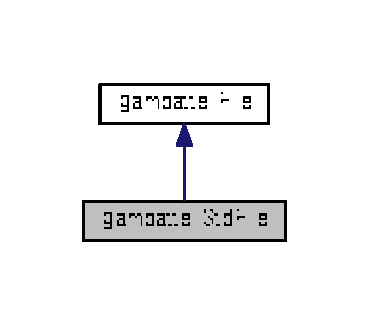
\includegraphics[width=177pt]{classgambatte_1_1StdFile__inherit__graph}
\end{center}
\end{figure}


Collaboration diagram for gambatte\+:\+:Std\+File\+:\nopagebreak
\begin{figure}[H]
\begin{center}
\leavevmode
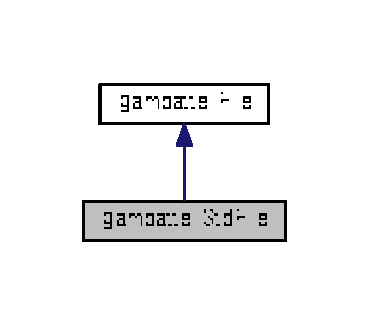
\includegraphics[width=177pt]{classgambatte_1_1StdFile__coll__graph}
\end{center}
\end{figure}
\subsection*{Public Member Functions}
\begin{DoxyCompactItemize}
\item 
\hyperlink{classgambatte_1_1StdFile_a9a170e2cfd76c7899f42e1e5cd4854f5}{Std\+File} (char const $\ast$\hyperlink{ioapi_8h_a7a03a664b090ce5c848ecb31cb4a2fa8}{filename})
\item 
virtual void \hyperlink{classgambatte_1_1StdFile_aa9f4ffbac979a4bf7607992eff78f469}{rewind} ()
\item 
virtual std\+::size\+\_\+t \hyperlink{classgambatte_1_1StdFile_aac486706e2f657b7396757ee9f8e7352}{size} () const
\item 
virtual void \hyperlink{classgambatte_1_1StdFile_a8c9c0994af30457e852ee887c1f9b38c}{read} (char $\ast$buffer, std\+::size\+\_\+t amount)
\item 
virtual bool \hyperlink{classgambatte_1_1StdFile_aa4f8f0f2854e3b11a71cb3d3109908eb}{fail} () const
\end{DoxyCompactItemize}
\subsection*{Private Attributes}
\begin{DoxyCompactItemize}
\item 
std\+::ifstream \hyperlink{classgambatte_1_1StdFile_a8a29b037eee32db589450ae81acdb5b9}{stream\+\_\+}
\item 
std\+::size\+\_\+t \hyperlink{classgambatte_1_1StdFile_a67ba9f58b97f9265a1db204638005a4d}{fsize\+\_\+}
\end{DoxyCompactItemize}


\subsection{Constructor \& Destructor Documentation}
\mbox{\Hypertarget{classgambatte_1_1StdFile_a9a170e2cfd76c7899f42e1e5cd4854f5}\label{classgambatte_1_1StdFile_a9a170e2cfd76c7899f42e1e5cd4854f5}} 
\index{gambatte\+::\+Std\+File@{gambatte\+::\+Std\+File}!Std\+File@{Std\+File}}
\index{Std\+File@{Std\+File}!gambatte\+::\+Std\+File@{gambatte\+::\+Std\+File}}
\subsubsection{\texorpdfstring{Std\+File()}{StdFile()}}
{\footnotesize\ttfamily gambatte\+::\+Std\+File\+::\+Std\+File (\begin{DoxyParamCaption}\item[{char const $\ast$}]{filename }\end{DoxyParamCaption})\hspace{0.3cm}{\ttfamily [inline]}, {\ttfamily [explicit]}}



\subsection{Member Function Documentation}
\mbox{\Hypertarget{classgambatte_1_1StdFile_aa4f8f0f2854e3b11a71cb3d3109908eb}\label{classgambatte_1_1StdFile_aa4f8f0f2854e3b11a71cb3d3109908eb}} 
\index{gambatte\+::\+Std\+File@{gambatte\+::\+Std\+File}!fail@{fail}}
\index{fail@{fail}!gambatte\+::\+Std\+File@{gambatte\+::\+Std\+File}}
\subsubsection{\texorpdfstring{fail()}{fail()}}
{\footnotesize\ttfamily virtual bool gambatte\+::\+Std\+File\+::fail (\begin{DoxyParamCaption}{ }\end{DoxyParamCaption}) const\hspace{0.3cm}{\ttfamily [inline]}, {\ttfamily [virtual]}}



Implements \hyperlink{classgambatte_1_1File_ac4e6a7055cd91176c9fb3e9215370c51}{gambatte\+::\+File}.

\mbox{\Hypertarget{classgambatte_1_1StdFile_a8c9c0994af30457e852ee887c1f9b38c}\label{classgambatte_1_1StdFile_a8c9c0994af30457e852ee887c1f9b38c}} 
\index{gambatte\+::\+Std\+File@{gambatte\+::\+Std\+File}!read@{read}}
\index{read@{read}!gambatte\+::\+Std\+File@{gambatte\+::\+Std\+File}}
\subsubsection{\texorpdfstring{read()}{read()}}
{\footnotesize\ttfamily virtual void gambatte\+::\+Std\+File\+::read (\begin{DoxyParamCaption}\item[{char $\ast$}]{buffer,  }\item[{std\+::size\+\_\+t}]{amount }\end{DoxyParamCaption})\hspace{0.3cm}{\ttfamily [inline]}, {\ttfamily [virtual]}}



Implements \hyperlink{classgambatte_1_1File_a58a6f97f55c93d15c9aa067d2a6db123}{gambatte\+::\+File}.

\mbox{\Hypertarget{classgambatte_1_1StdFile_aa9f4ffbac979a4bf7607992eff78f469}\label{classgambatte_1_1StdFile_aa9f4ffbac979a4bf7607992eff78f469}} 
\index{gambatte\+::\+Std\+File@{gambatte\+::\+Std\+File}!rewind@{rewind}}
\index{rewind@{rewind}!gambatte\+::\+Std\+File@{gambatte\+::\+Std\+File}}
\subsubsection{\texorpdfstring{rewind()}{rewind()}}
{\footnotesize\ttfamily virtual void gambatte\+::\+Std\+File\+::rewind (\begin{DoxyParamCaption}{ }\end{DoxyParamCaption})\hspace{0.3cm}{\ttfamily [inline]}, {\ttfamily [virtual]}}



Implements \hyperlink{classgambatte_1_1File_a37e873832be84757982d7a03662dfb95}{gambatte\+::\+File}.

\mbox{\Hypertarget{classgambatte_1_1StdFile_aac486706e2f657b7396757ee9f8e7352}\label{classgambatte_1_1StdFile_aac486706e2f657b7396757ee9f8e7352}} 
\index{gambatte\+::\+Std\+File@{gambatte\+::\+Std\+File}!size@{size}}
\index{size@{size}!gambatte\+::\+Std\+File@{gambatte\+::\+Std\+File}}
\subsubsection{\texorpdfstring{size()}{size()}}
{\footnotesize\ttfamily virtual std\+::size\+\_\+t gambatte\+::\+Std\+File\+::size (\begin{DoxyParamCaption}{ }\end{DoxyParamCaption}) const\hspace{0.3cm}{\ttfamily [inline]}, {\ttfamily [virtual]}}



Implements \hyperlink{classgambatte_1_1File_a589f615d436595eb97cbb9b9dc36632e}{gambatte\+::\+File}.



\subsection{Member Data Documentation}
\mbox{\Hypertarget{classgambatte_1_1StdFile_a67ba9f58b97f9265a1db204638005a4d}\label{classgambatte_1_1StdFile_a67ba9f58b97f9265a1db204638005a4d}} 
\index{gambatte\+::\+Std\+File@{gambatte\+::\+Std\+File}!fsize\+\_\+@{fsize\+\_\+}}
\index{fsize\+\_\+@{fsize\+\_\+}!gambatte\+::\+Std\+File@{gambatte\+::\+Std\+File}}
\subsubsection{\texorpdfstring{fsize\+\_\+}{fsize\_}}
{\footnotesize\ttfamily std\+::size\+\_\+t gambatte\+::\+Std\+File\+::fsize\+\_\+\hspace{0.3cm}{\ttfamily [private]}}

\mbox{\Hypertarget{classgambatte_1_1StdFile_a8a29b037eee32db589450ae81acdb5b9}\label{classgambatte_1_1StdFile_a8a29b037eee32db589450ae81acdb5b9}} 
\index{gambatte\+::\+Std\+File@{gambatte\+::\+Std\+File}!stream\+\_\+@{stream\+\_\+}}
\index{stream\+\_\+@{stream\+\_\+}!gambatte\+::\+Std\+File@{gambatte\+::\+Std\+File}}
\subsubsection{\texorpdfstring{stream\+\_\+}{stream\_}}
{\footnotesize\ttfamily std\+::ifstream gambatte\+::\+Std\+File\+::stream\+\_\+\hspace{0.3cm}{\ttfamily [private]}}



The documentation for this class was generated from the following file\+:\begin{DoxyCompactItemize}
\item 
src/file/\hyperlink{stdfile_8h}{stdfile.\+h}\end{DoxyCompactItemize}

\hypertarget{structMinKeeper_1_1Sum}{}\section{Min\+Keeper$<$ ids $>$\+:\+:Sum$<$ l $>$ Struct Template Reference}
\label{structMinKeeper_1_1Sum}\index{Min\+Keeper$<$ ids $>$\+::\+Sum$<$ l $>$@{Min\+Keeper$<$ ids $>$\+::\+Sum$<$ l $>$}}
\subsection*{Public Types}
\begin{DoxyCompactItemize}
\item 
enum \{ \hyperlink{structMinKeeper_1_1Sum_adce4c31739d72622c9de65c6d624b8aea5879f71c13fed43063fde60dc935dbf5}{r} = Min\+Keeper\+Util\+:\+:Sum$<$Num, l$>$\+:\+:r
 \}
\end{DoxyCompactItemize}


\subsection{Member Enumeration Documentation}
\mbox{\Hypertarget{structMinKeeper_1_1Sum_adce4c31739d72622c9de65c6d624b8ae}\label{structMinKeeper_1_1Sum_adce4c31739d72622c9de65c6d624b8ae}} 
\subsubsection{\texorpdfstring{anonymous enum}{anonymous enum}}
{\footnotesize\ttfamily template$<$int ids$>$ \\
template$<$int l$>$ \\
anonymous enum}

\begin{DoxyEnumFields}{Enumerator}
\raisebox{\heightof{T}}[0pt][0pt]{\index{r@{r}!Min\+Keeper\+::\+Sum@{Min\+Keeper\+::\+Sum}}\index{Min\+Keeper\+::\+Sum@{Min\+Keeper\+::\+Sum}!r@{r}}}\mbox{\Hypertarget{structMinKeeper_1_1Sum_adce4c31739d72622c9de65c6d624b8aea5879f71c13fed43063fde60dc935dbf5}\label{structMinKeeper_1_1Sum_adce4c31739d72622c9de65c6d624b8aea5879f71c13fed43063fde60dc935dbf5}} 
r&\\
\hline

\end{DoxyEnumFields}


The documentation for this struct was generated from the following file\+:\begin{DoxyCompactItemize}
\item 
src/\hyperlink{minkeeper_8h}{minkeeper.\+h}\end{DoxyCompactItemize}

\hypertarget{structMinKeeperUtil_1_1Sum}{}\section{Min\+Keeper\+Util\+:\+:Sum$<$ T, n $>$ Struct Template Reference}
\label{structMinKeeperUtil_1_1Sum}\index{Min\+Keeper\+Util\+::\+Sum$<$ T, n $>$@{Min\+Keeper\+Util\+::\+Sum$<$ T, n $>$}}


{\ttfamily \#include $<$minkeeper.\+h$>$}

\subsection*{Public Types}
\begin{DoxyCompactItemize}
\item 
enum \{ \hyperlink{structMinKeeperUtil_1_1Sum_a6067fd8cbcbcb5363d01e7178a52e72aaae2122fe450b3f2170a837544faeb000}{r} = T$<$n-\/1$>$\+:\+:r + Sum$<$T, n-\/1$>$\+:\+:r
 \}
\end{DoxyCompactItemize}


\subsection{Member Enumeration Documentation}
\mbox{\Hypertarget{structMinKeeperUtil_1_1Sum_a6067fd8cbcbcb5363d01e7178a52e72a}\label{structMinKeeperUtil_1_1Sum_a6067fd8cbcbcb5363d01e7178a52e72a}} 
\subsubsection{\texorpdfstring{anonymous enum}{anonymous enum}}
{\footnotesize\ttfamily template$<$template$<$ int $>$ class T, int n$>$ \\
anonymous enum}

\begin{DoxyEnumFields}{Enumerator}
\raisebox{\heightof{T}}[0pt][0pt]{\index{r@{r}!Min\+Keeper\+Util\+::\+Sum@{Min\+Keeper\+Util\+::\+Sum}}\index{Min\+Keeper\+Util\+::\+Sum@{Min\+Keeper\+Util\+::\+Sum}!r@{r}}}\mbox{\Hypertarget{structMinKeeperUtil_1_1Sum_a6067fd8cbcbcb5363d01e7178a52e72aaae2122fe450b3f2170a837544faeb000}\label{structMinKeeperUtil_1_1Sum_a6067fd8cbcbcb5363d01e7178a52e72aaae2122fe450b3f2170a837544faeb000}} 
r&\\
\hline

\end{DoxyEnumFields}


The documentation for this struct was generated from the following file\+:\begin{DoxyCompactItemize}
\item 
src/\hyperlink{minkeeper_8h}{minkeeper.\+h}\end{DoxyCompactItemize}

\hypertarget{structMinKeeperUtil_1_1Sum_3_01T_00_010_01_4}{}\section{Min\+Keeper\+Util\+:\+:Sum$<$ T, 0 $>$ Struct Template Reference}
\label{structMinKeeperUtil_1_1Sum_3_01T_00_010_01_4}\index{Min\+Keeper\+Util\+::\+Sum$<$ T, 0 $>$@{Min\+Keeper\+Util\+::\+Sum$<$ T, 0 $>$}}


{\ttfamily \#include $<$minkeeper.\+h$>$}

\subsection*{Public Types}
\begin{DoxyCompactItemize}
\item 
enum \{ \hyperlink{structMinKeeperUtil_1_1Sum_3_01T_00_010_01_4_a5b2093fddc1c5a07474a4b05727797cfa1a458b2b5354a0cefde69d7427d39eb0}{r} = 0
 \}
\end{DoxyCompactItemize}


\subsection{Member Enumeration Documentation}
\mbox{\Hypertarget{structMinKeeperUtil_1_1Sum_3_01T_00_010_01_4_a5b2093fddc1c5a07474a4b05727797cf}\label{structMinKeeperUtil_1_1Sum_3_01T_00_010_01_4_a5b2093fddc1c5a07474a4b05727797cf}} 
\subsubsection{\texorpdfstring{anonymous enum}{anonymous enum}}
{\footnotesize\ttfamily template$<$template$<$ int $>$ class T$>$ \\
anonymous enum}

\begin{DoxyEnumFields}{Enumerator}
\raisebox{\heightof{T}}[0pt][0pt]{\index{r@{r}!Min\+Keeper\+Util\+::\+Sum$<$ T, 0 $>$@{Min\+Keeper\+Util\+::\+Sum$<$ T, 0 $>$}}\index{Min\+Keeper\+Util\+::\+Sum$<$ T, 0 $>$@{Min\+Keeper\+Util\+::\+Sum$<$ T, 0 $>$}!r@{r}}}\mbox{\Hypertarget{structMinKeeperUtil_1_1Sum_3_01T_00_010_01_4_a5b2093fddc1c5a07474a4b05727797cfa1a458b2b5354a0cefde69d7427d39eb0}\label{structMinKeeperUtil_1_1Sum_3_01T_00_010_01_4_a5b2093fddc1c5a07474a4b05727797cfa1a458b2b5354a0cefde69d7427d39eb0}} 
r&\\
\hline

\end{DoxyEnumFields}


The documentation for this struct was generated from the following file\+:\begin{DoxyCompactItemize}
\item 
src/\hyperlink{minkeeper_8h}{minkeeper.\+h}\end{DoxyCompactItemize}

\hypertarget{classgambatte_1_1Channel1_1_1SweepUnit}{}\section{gambatte\+:\+:Channel1\+:\+:Sweep\+Unit Class Reference}
\label{classgambatte_1_1Channel1_1_1SweepUnit}\index{gambatte\+::\+Channel1\+::\+Sweep\+Unit@{gambatte\+::\+Channel1\+::\+Sweep\+Unit}}


Inheritance diagram for gambatte\+:\+:Channel1\+:\+:Sweep\+Unit\+:
\nopagebreak
\begin{figure}[H]
\begin{center}
\leavevmode
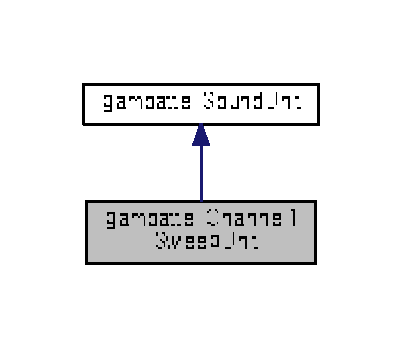
\includegraphics[width=193pt]{classgambatte_1_1Channel1_1_1SweepUnit__inherit__graph}
\end{center}
\end{figure}


Collaboration diagram for gambatte\+:\+:Channel1\+:\+:Sweep\+Unit\+:
\nopagebreak
\begin{figure}[H]
\begin{center}
\leavevmode
\includegraphics[width=350pt]{classgambatte_1_1Channel1_1_1SweepUnit__coll__graph}
\end{center}
\end{figure}
\subsection*{Public Member Functions}
\begin{DoxyCompactItemize}
\item 
\hyperlink{classgambatte_1_1Channel1_1_1SweepUnit_a1b12e2135d03fe19b7b20d5f7884c2d8}{Sweep\+Unit} (\hyperlink{classgambatte_1_1MasterDisabler}{Master\+Disabler} \&disabler, \hyperlink{classgambatte_1_1DutyUnit}{Duty\+Unit} \&duty\+Unit)
\item 
virtual void \hyperlink{classgambatte_1_1Channel1_1_1SweepUnit_a17c182372fc3f4aaf845ab89cf20201d}{event} ()
\item 
void \hyperlink{classgambatte_1_1Channel1_1_1SweepUnit_a61a441938851b0f4b2c8e7dfc1f2a7fa}{nr0\+Change} (unsigned new\+Nr0)
\item 
void \hyperlink{classgambatte_1_1Channel1_1_1SweepUnit_a2428c20b75eb4d571eb4d6979e15949d}{nr4\+Init} (unsigned cycle\+Counter)
\item 
void \hyperlink{classgambatte_1_1Channel1_1_1SweepUnit_a6aef2b1067cfc9f032b6d386c97ed2bb}{reset} ()
\item 
void \hyperlink{classgambatte_1_1Channel1_1_1SweepUnit_a5d957523fd18c30eb42d47c89fe01a13}{save\+State} (\hyperlink{structgambatte_1_1SaveState}{Save\+State} \&\hyperlink{ppu_8cpp_a2f2eca6997ee7baf8901725ae074d45b}{state}) const
\item 
void \hyperlink{classgambatte_1_1Channel1_1_1SweepUnit_a878dc87fd614f8cec90fdccb55e56736}{load\+State} (\hyperlink{structgambatte_1_1SaveState}{Save\+State} const \&\hyperlink{ppu_8cpp_a2f2eca6997ee7baf8901725ae074d45b}{state})
\item 
void \hyperlink{classgambatte_1_1Channel1_1_1SweepUnit_aad7f6073e9f8ab5faf059ee1b4659e7b}{load\+Or\+Save} (\hyperlink{classgambatte_1_1loadsave}{loadsave} \&\hyperlink{ppu_8cpp_a2f2eca6997ee7baf8901725ae074d45b}{state})
\end{DoxyCompactItemize}
\subsection*{Private Member Functions}
\begin{DoxyCompactItemize}
\item 
unsigned \hyperlink{classgambatte_1_1Channel1_1_1SweepUnit_ad5b8441b3bc35077ace9f661f4128a4d}{calc\+Freq} ()
\end{DoxyCompactItemize}
\subsection*{Private Attributes}
\begin{DoxyCompactItemize}
\item 
\hyperlink{classgambatte_1_1MasterDisabler}{Master\+Disabler} \& \hyperlink{classgambatte_1_1Channel1_1_1SweepUnit_a6ccec31d73ac308e0801d2c95a3970d8}{disable\+Master\+\_\+}
\item 
\hyperlink{classgambatte_1_1DutyUnit}{Duty\+Unit} \& \hyperlink{classgambatte_1_1Channel1_1_1SweepUnit_a267cbe2007d0b13e7659a82f40c24544}{duty\+Unit\+\_\+}
\item 
unsigned short \hyperlink{classgambatte_1_1Channel1_1_1SweepUnit_af1861651dc7a6a7dde893a1df498771d}{shadow\+\_\+}
\item 
unsigned char \hyperlink{classgambatte_1_1Channel1_1_1SweepUnit_ab7e9cf92f0d9efca5a51774dbc37a985}{nr0\+\_\+}
\item 
bool \hyperlink{classgambatte_1_1Channel1_1_1SweepUnit_a288f0ab06ac66c247ca17002e230ae1e}{negging\+\_\+}
\end{DoxyCompactItemize}
\subsection*{Additional Inherited Members}


\subsection{Constructor \& Destructor Documentation}
\mbox{\Hypertarget{classgambatte_1_1Channel1_1_1SweepUnit_a1b12e2135d03fe19b7b20d5f7884c2d8}\label{classgambatte_1_1Channel1_1_1SweepUnit_a1b12e2135d03fe19b7b20d5f7884c2d8}} 
\index{gambatte\+::\+Channel1\+::\+Sweep\+Unit@{gambatte\+::\+Channel1\+::\+Sweep\+Unit}!Sweep\+Unit@{Sweep\+Unit}}
\index{Sweep\+Unit@{Sweep\+Unit}!gambatte\+::\+Channel1\+::\+Sweep\+Unit@{gambatte\+::\+Channel1\+::\+Sweep\+Unit}}
\subsubsection{\texorpdfstring{Sweep\+Unit()}{SweepUnit()}}
{\footnotesize\ttfamily gambatte\+::\+Channel1\+::\+Sweep\+Unit\+::\+Sweep\+Unit (\begin{DoxyParamCaption}\item[{\hyperlink{classgambatte_1_1MasterDisabler}{Master\+Disabler} \&}]{disabler,  }\item[{\hyperlink{classgambatte_1_1DutyUnit}{Duty\+Unit} \&}]{duty\+Unit }\end{DoxyParamCaption})}



\subsection{Member Function Documentation}
\mbox{\Hypertarget{classgambatte_1_1Channel1_1_1SweepUnit_ad5b8441b3bc35077ace9f661f4128a4d}\label{classgambatte_1_1Channel1_1_1SweepUnit_ad5b8441b3bc35077ace9f661f4128a4d}} 
\index{gambatte\+::\+Channel1\+::\+Sweep\+Unit@{gambatte\+::\+Channel1\+::\+Sweep\+Unit}!calc\+Freq@{calc\+Freq}}
\index{calc\+Freq@{calc\+Freq}!gambatte\+::\+Channel1\+::\+Sweep\+Unit@{gambatte\+::\+Channel1\+::\+Sweep\+Unit}}
\subsubsection{\texorpdfstring{calc\+Freq()}{calcFreq()}}
{\footnotesize\ttfamily unsigned gambatte\+::\+Channel1\+::\+Sweep\+Unit\+::calc\+Freq (\begin{DoxyParamCaption}{ }\end{DoxyParamCaption})\hspace{0.3cm}{\ttfamily [private]}}

\mbox{\Hypertarget{classgambatte_1_1Channel1_1_1SweepUnit_a17c182372fc3f4aaf845ab89cf20201d}\label{classgambatte_1_1Channel1_1_1SweepUnit_a17c182372fc3f4aaf845ab89cf20201d}} 
\index{gambatte\+::\+Channel1\+::\+Sweep\+Unit@{gambatte\+::\+Channel1\+::\+Sweep\+Unit}!event@{event}}
\index{event@{event}!gambatte\+::\+Channel1\+::\+Sweep\+Unit@{gambatte\+::\+Channel1\+::\+Sweep\+Unit}}
\subsubsection{\texorpdfstring{event()}{event()}}
{\footnotesize\ttfamily void gambatte\+::\+Channel1\+::\+Sweep\+Unit\+::event (\begin{DoxyParamCaption}{ }\end{DoxyParamCaption})\hspace{0.3cm}{\ttfamily [virtual]}}



Implements \hyperlink{classgambatte_1_1SoundUnit_a8ad6df87fc3700d9d3bee470383197b4}{gambatte\+::\+Sound\+Unit}.

\mbox{\Hypertarget{classgambatte_1_1Channel1_1_1SweepUnit_aad7f6073e9f8ab5faf059ee1b4659e7b}\label{classgambatte_1_1Channel1_1_1SweepUnit_aad7f6073e9f8ab5faf059ee1b4659e7b}} 
\index{gambatte\+::\+Channel1\+::\+Sweep\+Unit@{gambatte\+::\+Channel1\+::\+Sweep\+Unit}!load\+Or\+Save@{load\+Or\+Save}}
\index{load\+Or\+Save@{load\+Or\+Save}!gambatte\+::\+Channel1\+::\+Sweep\+Unit@{gambatte\+::\+Channel1\+::\+Sweep\+Unit}}
\subsubsection{\texorpdfstring{load\+Or\+Save()}{loadOrSave()}}
{\footnotesize\ttfamily void gambatte\+::\+Channel1\+::\+Sweep\+Unit\+::load\+Or\+Save (\begin{DoxyParamCaption}\item[{\hyperlink{classgambatte_1_1loadsave}{loadsave} \&}]{state }\end{DoxyParamCaption})\hspace{0.3cm}{\ttfamily [inline]}}

\mbox{\Hypertarget{classgambatte_1_1Channel1_1_1SweepUnit_a878dc87fd614f8cec90fdccb55e56736}\label{classgambatte_1_1Channel1_1_1SweepUnit_a878dc87fd614f8cec90fdccb55e56736}} 
\index{gambatte\+::\+Channel1\+::\+Sweep\+Unit@{gambatte\+::\+Channel1\+::\+Sweep\+Unit}!load\+State@{load\+State}}
\index{load\+State@{load\+State}!gambatte\+::\+Channel1\+::\+Sweep\+Unit@{gambatte\+::\+Channel1\+::\+Sweep\+Unit}}
\subsubsection{\texorpdfstring{load\+State()}{loadState()}}
{\footnotesize\ttfamily void gambatte\+::\+Channel1\+::\+Sweep\+Unit\+::load\+State (\begin{DoxyParamCaption}\item[{\hyperlink{structgambatte_1_1SaveState}{Save\+State} const \&}]{state }\end{DoxyParamCaption})}

\mbox{\Hypertarget{classgambatte_1_1Channel1_1_1SweepUnit_a61a441938851b0f4b2c8e7dfc1f2a7fa}\label{classgambatte_1_1Channel1_1_1SweepUnit_a61a441938851b0f4b2c8e7dfc1f2a7fa}} 
\index{gambatte\+::\+Channel1\+::\+Sweep\+Unit@{gambatte\+::\+Channel1\+::\+Sweep\+Unit}!nr0\+Change@{nr0\+Change}}
\index{nr0\+Change@{nr0\+Change}!gambatte\+::\+Channel1\+::\+Sweep\+Unit@{gambatte\+::\+Channel1\+::\+Sweep\+Unit}}
\subsubsection{\texorpdfstring{nr0\+Change()}{nr0Change()}}
{\footnotesize\ttfamily void gambatte\+::\+Channel1\+::\+Sweep\+Unit\+::nr0\+Change (\begin{DoxyParamCaption}\item[{unsigned}]{new\+Nr0 }\end{DoxyParamCaption})}

\mbox{\Hypertarget{classgambatte_1_1Channel1_1_1SweepUnit_a2428c20b75eb4d571eb4d6979e15949d}\label{classgambatte_1_1Channel1_1_1SweepUnit_a2428c20b75eb4d571eb4d6979e15949d}} 
\index{gambatte\+::\+Channel1\+::\+Sweep\+Unit@{gambatte\+::\+Channel1\+::\+Sweep\+Unit}!nr4\+Init@{nr4\+Init}}
\index{nr4\+Init@{nr4\+Init}!gambatte\+::\+Channel1\+::\+Sweep\+Unit@{gambatte\+::\+Channel1\+::\+Sweep\+Unit}}
\subsubsection{\texorpdfstring{nr4\+Init()}{nr4Init()}}
{\footnotesize\ttfamily void gambatte\+::\+Channel1\+::\+Sweep\+Unit\+::nr4\+Init (\begin{DoxyParamCaption}\item[{unsigned}]{cycle\+Counter }\end{DoxyParamCaption})}

\mbox{\Hypertarget{classgambatte_1_1Channel1_1_1SweepUnit_a6aef2b1067cfc9f032b6d386c97ed2bb}\label{classgambatte_1_1Channel1_1_1SweepUnit_a6aef2b1067cfc9f032b6d386c97ed2bb}} 
\index{gambatte\+::\+Channel1\+::\+Sweep\+Unit@{gambatte\+::\+Channel1\+::\+Sweep\+Unit}!reset@{reset}}
\index{reset@{reset}!gambatte\+::\+Channel1\+::\+Sweep\+Unit@{gambatte\+::\+Channel1\+::\+Sweep\+Unit}}
\subsubsection{\texorpdfstring{reset()}{reset()}}
{\footnotesize\ttfamily void gambatte\+::\+Channel1\+::\+Sweep\+Unit\+::reset (\begin{DoxyParamCaption}{ }\end{DoxyParamCaption})}

\mbox{\Hypertarget{classgambatte_1_1Channel1_1_1SweepUnit_a5d957523fd18c30eb42d47c89fe01a13}\label{classgambatte_1_1Channel1_1_1SweepUnit_a5d957523fd18c30eb42d47c89fe01a13}} 
\index{gambatte\+::\+Channel1\+::\+Sweep\+Unit@{gambatte\+::\+Channel1\+::\+Sweep\+Unit}!save\+State@{save\+State}}
\index{save\+State@{save\+State}!gambatte\+::\+Channel1\+::\+Sweep\+Unit@{gambatte\+::\+Channel1\+::\+Sweep\+Unit}}
\subsubsection{\texorpdfstring{save\+State()}{saveState()}}
{\footnotesize\ttfamily void gambatte\+::\+Channel1\+::\+Sweep\+Unit\+::save\+State (\begin{DoxyParamCaption}\item[{\hyperlink{structgambatte_1_1SaveState}{Save\+State} \&}]{state }\end{DoxyParamCaption}) const}



\subsection{Member Data Documentation}
\mbox{\Hypertarget{classgambatte_1_1Channel1_1_1SweepUnit_a6ccec31d73ac308e0801d2c95a3970d8}\label{classgambatte_1_1Channel1_1_1SweepUnit_a6ccec31d73ac308e0801d2c95a3970d8}} 
\index{gambatte\+::\+Channel1\+::\+Sweep\+Unit@{gambatte\+::\+Channel1\+::\+Sweep\+Unit}!disable\+Master\+\_\+@{disable\+Master\+\_\+}}
\index{disable\+Master\+\_\+@{disable\+Master\+\_\+}!gambatte\+::\+Channel1\+::\+Sweep\+Unit@{gambatte\+::\+Channel1\+::\+Sweep\+Unit}}
\subsubsection{\texorpdfstring{disable\+Master\+\_\+}{disableMaster\_}}
{\footnotesize\ttfamily \hyperlink{classgambatte_1_1MasterDisabler}{Master\+Disabler}\& gambatte\+::\+Channel1\+::\+Sweep\+Unit\+::disable\+Master\+\_\+\hspace{0.3cm}{\ttfamily [private]}}

\mbox{\Hypertarget{classgambatte_1_1Channel1_1_1SweepUnit_a267cbe2007d0b13e7659a82f40c24544}\label{classgambatte_1_1Channel1_1_1SweepUnit_a267cbe2007d0b13e7659a82f40c24544}} 
\index{gambatte\+::\+Channel1\+::\+Sweep\+Unit@{gambatte\+::\+Channel1\+::\+Sweep\+Unit}!duty\+Unit\+\_\+@{duty\+Unit\+\_\+}}
\index{duty\+Unit\+\_\+@{duty\+Unit\+\_\+}!gambatte\+::\+Channel1\+::\+Sweep\+Unit@{gambatte\+::\+Channel1\+::\+Sweep\+Unit}}
\subsubsection{\texorpdfstring{duty\+Unit\+\_\+}{dutyUnit\_}}
{\footnotesize\ttfamily \hyperlink{classgambatte_1_1DutyUnit}{Duty\+Unit}\& gambatte\+::\+Channel1\+::\+Sweep\+Unit\+::duty\+Unit\+\_\+\hspace{0.3cm}{\ttfamily [private]}}

\mbox{\Hypertarget{classgambatte_1_1Channel1_1_1SweepUnit_a288f0ab06ac66c247ca17002e230ae1e}\label{classgambatte_1_1Channel1_1_1SweepUnit_a288f0ab06ac66c247ca17002e230ae1e}} 
\index{gambatte\+::\+Channel1\+::\+Sweep\+Unit@{gambatte\+::\+Channel1\+::\+Sweep\+Unit}!negging\+\_\+@{negging\+\_\+}}
\index{negging\+\_\+@{negging\+\_\+}!gambatte\+::\+Channel1\+::\+Sweep\+Unit@{gambatte\+::\+Channel1\+::\+Sweep\+Unit}}
\subsubsection{\texorpdfstring{negging\+\_\+}{negging\_}}
{\footnotesize\ttfamily bool gambatte\+::\+Channel1\+::\+Sweep\+Unit\+::negging\+\_\+\hspace{0.3cm}{\ttfamily [private]}}

\mbox{\Hypertarget{classgambatte_1_1Channel1_1_1SweepUnit_ab7e9cf92f0d9efca5a51774dbc37a985}\label{classgambatte_1_1Channel1_1_1SweepUnit_ab7e9cf92f0d9efca5a51774dbc37a985}} 
\index{gambatte\+::\+Channel1\+::\+Sweep\+Unit@{gambatte\+::\+Channel1\+::\+Sweep\+Unit}!nr0\+\_\+@{nr0\+\_\+}}
\index{nr0\+\_\+@{nr0\+\_\+}!gambatte\+::\+Channel1\+::\+Sweep\+Unit@{gambatte\+::\+Channel1\+::\+Sweep\+Unit}}
\subsubsection{\texorpdfstring{nr0\+\_\+}{nr0\_}}
{\footnotesize\ttfamily unsigned char gambatte\+::\+Channel1\+::\+Sweep\+Unit\+::nr0\+\_\+\hspace{0.3cm}{\ttfamily [private]}}

\mbox{\Hypertarget{classgambatte_1_1Channel1_1_1SweepUnit_af1861651dc7a6a7dde893a1df498771d}\label{classgambatte_1_1Channel1_1_1SweepUnit_af1861651dc7a6a7dde893a1df498771d}} 
\index{gambatte\+::\+Channel1\+::\+Sweep\+Unit@{gambatte\+::\+Channel1\+::\+Sweep\+Unit}!shadow\+\_\+@{shadow\+\_\+}}
\index{shadow\+\_\+@{shadow\+\_\+}!gambatte\+::\+Channel1\+::\+Sweep\+Unit@{gambatte\+::\+Channel1\+::\+Sweep\+Unit}}
\subsubsection{\texorpdfstring{shadow\+\_\+}{shadow\_}}
{\footnotesize\ttfamily unsigned short gambatte\+::\+Channel1\+::\+Sweep\+Unit\+::shadow\+\_\+\hspace{0.3cm}{\ttfamily [private]}}



The documentation for this class was generated from the following files\+:\begin{DoxyCompactItemize}
\item 
src/sound/\hyperlink{channel1_8h}{channel1.\+h}\item 
src/sound/\hyperlink{channel1_8cpp}{channel1.\+cpp}\end{DoxyCompactItemize}

\hypertarget{classgambatte_1_1Tima}{}\section{gambatte\+:\+:Tima Class Reference}
\label{classgambatte_1_1Tima}\index{gambatte\+::\+Tima@{gambatte\+::\+Tima}}


{\ttfamily \#include $<$tima.\+h$>$}

\subsection*{Public Member Functions}
\begin{DoxyCompactItemize}
\item 
\hyperlink{classgambatte_1_1Tima_a335d610e3c5aeef9f80b7693d414d42e}{Tima} ()
\item 
void \hyperlink{classgambatte_1_1Tima_a40d563556152c52bbd838d70895e4be4}{save\+State} (\hyperlink{structgambatte_1_1SaveState}{Save\+State} \&) const
\item 
void \hyperlink{classgambatte_1_1Tima_a5754a2d76e158ed3cae830cb52cc58c3}{load\+State} (const \hyperlink{structgambatte_1_1SaveState}{Save\+State} \&, \hyperlink{classgambatte_1_1TimaInterruptRequester}{Tima\+Interrupt\+Requester} tima\+Irq)
\item 
void \hyperlink{classgambatte_1_1Tima_ae79b79227e0c0ace7d1dd173ae525b27}{reset\+Cc} (unsigned old\+Cc, unsigned new\+Cc, \hyperlink{classgambatte_1_1TimaInterruptRequester}{Tima\+Interrupt\+Requester} tima\+Irq)
\item 
void \hyperlink{classgambatte_1_1Tima_a6b9a6fd1515acfb8d0b1315da7883e51}{set\+Tima} (unsigned \hyperlink{classgambatte_1_1Tima_a73338015ebd3d2d5a00e7d2554c2f3c5}{tima}, unsigned cc, \hyperlink{classgambatte_1_1TimaInterruptRequester}{Tima\+Interrupt\+Requester} tima\+Irq)
\item 
void \hyperlink{classgambatte_1_1Tima_a937b897a30ad1289069716b309555dd4}{set\+Tma} (unsigned tma, unsigned cc, \hyperlink{classgambatte_1_1TimaInterruptRequester}{Tima\+Interrupt\+Requester} tima\+Irq)
\item 
void \hyperlink{classgambatte_1_1Tima_a1e9e5f8cd0e04e5f73eafbf364bef772}{set\+Tac} (unsigned tac, unsigned cc, \hyperlink{classgambatte_1_1TimaInterruptRequester}{Tima\+Interrupt\+Requester} tima\+Irq)
\item 
unsigned \hyperlink{classgambatte_1_1Tima_a73338015ebd3d2d5a00e7d2554c2f3c5}{tima} (unsigned cc)
\item 
void \hyperlink{classgambatte_1_1Tima_a9bf4e6fead69bda13cab7e7565d1c414}{do\+Irq\+Event} (\hyperlink{classgambatte_1_1TimaInterruptRequester}{Tima\+Interrupt\+Requester} tima\+Irq)
\item 
void \hyperlink{classgambatte_1_1Tima_af5bd0ed8cd9d288a87ee8530cd39bf39}{update\+Tima} (unsigned cc)
\item 
void \hyperlink{classgambatte_1_1Tima_a42f102eee85822ce7b484679d9d36132}{load\+Or\+Save} (\hyperlink{classgambatte_1_1loadsave}{loadsave} \&\hyperlink{ppu_8cpp_a2f2eca6997ee7baf8901725ae074d45b}{state})
\end{DoxyCompactItemize}
\subsection*{Private Member Functions}
\begin{DoxyCompactItemize}
\item 
void \hyperlink{classgambatte_1_1Tima_adbbd88e7c35830157e60ee06e7f4dc05}{update\+Irq} (unsigned const cc, \hyperlink{classgambatte_1_1TimaInterruptRequester}{Tima\+Interrupt\+Requester} tima\+Irq)
\end{DoxyCompactItemize}
\subsection*{Private Attributes}
\begin{DoxyCompactItemize}
\item 
unsigned \hyperlink{classgambatte_1_1Tima_ac448ab51bb8f7d47927f86a238513238}{last\+Update\+\_\+}
\item 
unsigned \hyperlink{classgambatte_1_1Tima_a7badef965f06c5b99ab6c90216b6d67b}{tmatime\+\_\+}
\item 
unsigned char \hyperlink{classgambatte_1_1Tima_afe4fa0fb57c9c5a5a0218bdd1d440c89}{tima\+\_\+}
\item 
unsigned char \hyperlink{classgambatte_1_1Tima_ab7d524d7391f3450e7e3a5477dead85c}{tma\+\_\+}
\item 
unsigned char \hyperlink{classgambatte_1_1Tima_a85c00bd12ac64c4a334de4f08032cb9f}{tac\+\_\+}
\end{DoxyCompactItemize}


\subsection{Constructor \& Destructor Documentation}
\mbox{\Hypertarget{classgambatte_1_1Tima_a335d610e3c5aeef9f80b7693d414d42e}\label{classgambatte_1_1Tima_a335d610e3c5aeef9f80b7693d414d42e}} 
\index{gambatte\+::\+Tima@{gambatte\+::\+Tima}!Tima@{Tima}}
\index{Tima@{Tima}!gambatte\+::\+Tima@{gambatte\+::\+Tima}}
\subsubsection{\texorpdfstring{Tima()}{Tima()}}
{\footnotesize\ttfamily gambatte\+::\+Tima\+::\+Tima (\begin{DoxyParamCaption}{ }\end{DoxyParamCaption})}



\subsection{Member Function Documentation}
\mbox{\Hypertarget{classgambatte_1_1Tima_a9bf4e6fead69bda13cab7e7565d1c414}\label{classgambatte_1_1Tima_a9bf4e6fead69bda13cab7e7565d1c414}} 
\index{gambatte\+::\+Tima@{gambatte\+::\+Tima}!do\+Irq\+Event@{do\+Irq\+Event}}
\index{do\+Irq\+Event@{do\+Irq\+Event}!gambatte\+::\+Tima@{gambatte\+::\+Tima}}
\subsubsection{\texorpdfstring{do\+Irq\+Event()}{doIrqEvent()}}
{\footnotesize\ttfamily void gambatte\+::\+Tima\+::do\+Irq\+Event (\begin{DoxyParamCaption}\item[{\hyperlink{classgambatte_1_1TimaInterruptRequester}{Tima\+Interrupt\+Requester}}]{tima\+Irq }\end{DoxyParamCaption})}

\mbox{\Hypertarget{classgambatte_1_1Tima_a42f102eee85822ce7b484679d9d36132}\label{classgambatte_1_1Tima_a42f102eee85822ce7b484679d9d36132}} 
\index{gambatte\+::\+Tima@{gambatte\+::\+Tima}!load\+Or\+Save@{load\+Or\+Save}}
\index{load\+Or\+Save@{load\+Or\+Save}!gambatte\+::\+Tima@{gambatte\+::\+Tima}}
\subsubsection{\texorpdfstring{load\+Or\+Save()}{loadOrSave()}}
{\footnotesize\ttfamily void gambatte\+::\+Tima\+::load\+Or\+Save (\begin{DoxyParamCaption}\item[{\hyperlink{classgambatte_1_1loadsave}{loadsave} \&}]{state }\end{DoxyParamCaption})}

\mbox{\Hypertarget{classgambatte_1_1Tima_a5754a2d76e158ed3cae830cb52cc58c3}\label{classgambatte_1_1Tima_a5754a2d76e158ed3cae830cb52cc58c3}} 
\index{gambatte\+::\+Tima@{gambatte\+::\+Tima}!load\+State@{load\+State}}
\index{load\+State@{load\+State}!gambatte\+::\+Tima@{gambatte\+::\+Tima}}
\subsubsection{\texorpdfstring{load\+State()}{loadState()}}
{\footnotesize\ttfamily void gambatte\+::\+Tima\+::load\+State (\begin{DoxyParamCaption}\item[{const \hyperlink{structgambatte_1_1SaveState}{Save\+State} \&}]{state,  }\item[{\hyperlink{classgambatte_1_1TimaInterruptRequester}{Tima\+Interrupt\+Requester}}]{tima\+Irq }\end{DoxyParamCaption})}

\mbox{\Hypertarget{classgambatte_1_1Tima_ae79b79227e0c0ace7d1dd173ae525b27}\label{classgambatte_1_1Tima_ae79b79227e0c0ace7d1dd173ae525b27}} 
\index{gambatte\+::\+Tima@{gambatte\+::\+Tima}!reset\+Cc@{reset\+Cc}}
\index{reset\+Cc@{reset\+Cc}!gambatte\+::\+Tima@{gambatte\+::\+Tima}}
\subsubsection{\texorpdfstring{reset\+Cc()}{resetCc()}}
{\footnotesize\ttfamily void gambatte\+::\+Tima\+::reset\+Cc (\begin{DoxyParamCaption}\item[{unsigned}]{old\+Cc,  }\item[{unsigned}]{new\+Cc,  }\item[{\hyperlink{classgambatte_1_1TimaInterruptRequester}{Tima\+Interrupt\+Requester}}]{tima\+Irq }\end{DoxyParamCaption})}

\mbox{\Hypertarget{classgambatte_1_1Tima_a40d563556152c52bbd838d70895e4be4}\label{classgambatte_1_1Tima_a40d563556152c52bbd838d70895e4be4}} 
\index{gambatte\+::\+Tima@{gambatte\+::\+Tima}!save\+State@{save\+State}}
\index{save\+State@{save\+State}!gambatte\+::\+Tima@{gambatte\+::\+Tima}}
\subsubsection{\texorpdfstring{save\+State()}{saveState()}}
{\footnotesize\ttfamily void gambatte\+::\+Tima\+::save\+State (\begin{DoxyParamCaption}\item[{\hyperlink{structgambatte_1_1SaveState}{Save\+State} \&}]{state }\end{DoxyParamCaption}) const}

\mbox{\Hypertarget{classgambatte_1_1Tima_a1e9e5f8cd0e04e5f73eafbf364bef772}\label{classgambatte_1_1Tima_a1e9e5f8cd0e04e5f73eafbf364bef772}} 
\index{gambatte\+::\+Tima@{gambatte\+::\+Tima}!set\+Tac@{set\+Tac}}
\index{set\+Tac@{set\+Tac}!gambatte\+::\+Tima@{gambatte\+::\+Tima}}
\subsubsection{\texorpdfstring{set\+Tac()}{setTac()}}
{\footnotesize\ttfamily void gambatte\+::\+Tima\+::set\+Tac (\begin{DoxyParamCaption}\item[{unsigned}]{tac,  }\item[{unsigned}]{cc,  }\item[{\hyperlink{classgambatte_1_1TimaInterruptRequester}{Tima\+Interrupt\+Requester}}]{tima\+Irq }\end{DoxyParamCaption})}

\mbox{\Hypertarget{classgambatte_1_1Tima_a6b9a6fd1515acfb8d0b1315da7883e51}\label{classgambatte_1_1Tima_a6b9a6fd1515acfb8d0b1315da7883e51}} 
\index{gambatte\+::\+Tima@{gambatte\+::\+Tima}!set\+Tima@{set\+Tima}}
\index{set\+Tima@{set\+Tima}!gambatte\+::\+Tima@{gambatte\+::\+Tima}}
\subsubsection{\texorpdfstring{set\+Tima()}{setTima()}}
{\footnotesize\ttfamily void gambatte\+::\+Tima\+::set\+Tima (\begin{DoxyParamCaption}\item[{unsigned}]{tima,  }\item[{unsigned}]{cc,  }\item[{\hyperlink{classgambatte_1_1TimaInterruptRequester}{Tima\+Interrupt\+Requester}}]{tima\+Irq }\end{DoxyParamCaption})}

\mbox{\Hypertarget{classgambatte_1_1Tima_a937b897a30ad1289069716b309555dd4}\label{classgambatte_1_1Tima_a937b897a30ad1289069716b309555dd4}} 
\index{gambatte\+::\+Tima@{gambatte\+::\+Tima}!set\+Tma@{set\+Tma}}
\index{set\+Tma@{set\+Tma}!gambatte\+::\+Tima@{gambatte\+::\+Tima}}
\subsubsection{\texorpdfstring{set\+Tma()}{setTma()}}
{\footnotesize\ttfamily void gambatte\+::\+Tima\+::set\+Tma (\begin{DoxyParamCaption}\item[{unsigned}]{tma,  }\item[{unsigned}]{cc,  }\item[{\hyperlink{classgambatte_1_1TimaInterruptRequester}{Tima\+Interrupt\+Requester}}]{tima\+Irq }\end{DoxyParamCaption})}

\mbox{\Hypertarget{classgambatte_1_1Tima_a73338015ebd3d2d5a00e7d2554c2f3c5}\label{classgambatte_1_1Tima_a73338015ebd3d2d5a00e7d2554c2f3c5}} 
\index{gambatte\+::\+Tima@{gambatte\+::\+Tima}!tima@{tima}}
\index{tima@{tima}!gambatte\+::\+Tima@{gambatte\+::\+Tima}}
\subsubsection{\texorpdfstring{tima()}{tima()}}
{\footnotesize\ttfamily unsigned gambatte\+::\+Tima\+::tima (\begin{DoxyParamCaption}\item[{unsigned}]{cc }\end{DoxyParamCaption})}

\mbox{\Hypertarget{classgambatte_1_1Tima_adbbd88e7c35830157e60ee06e7f4dc05}\label{classgambatte_1_1Tima_adbbd88e7c35830157e60ee06e7f4dc05}} 
\index{gambatte\+::\+Tima@{gambatte\+::\+Tima}!update\+Irq@{update\+Irq}}
\index{update\+Irq@{update\+Irq}!gambatte\+::\+Tima@{gambatte\+::\+Tima}}
\subsubsection{\texorpdfstring{update\+Irq()}{updateIrq()}}
{\footnotesize\ttfamily void gambatte\+::\+Tima\+::update\+Irq (\begin{DoxyParamCaption}\item[{unsigned const}]{cc,  }\item[{\hyperlink{classgambatte_1_1TimaInterruptRequester}{Tima\+Interrupt\+Requester}}]{tima\+Irq }\end{DoxyParamCaption})\hspace{0.3cm}{\ttfamily [inline]}, {\ttfamily [private]}}

\mbox{\Hypertarget{classgambatte_1_1Tima_af5bd0ed8cd9d288a87ee8530cd39bf39}\label{classgambatte_1_1Tima_af5bd0ed8cd9d288a87ee8530cd39bf39}} 
\index{gambatte\+::\+Tima@{gambatte\+::\+Tima}!update\+Tima@{update\+Tima}}
\index{update\+Tima@{update\+Tima}!gambatte\+::\+Tima@{gambatte\+::\+Tima}}
\subsubsection{\texorpdfstring{update\+Tima()}{updateTima()}}
{\footnotesize\ttfamily void gambatte\+::\+Tima\+::update\+Tima (\begin{DoxyParamCaption}\item[{unsigned}]{cc }\end{DoxyParamCaption})}



\subsection{Member Data Documentation}
\mbox{\Hypertarget{classgambatte_1_1Tima_ac448ab51bb8f7d47927f86a238513238}\label{classgambatte_1_1Tima_ac448ab51bb8f7d47927f86a238513238}} 
\index{gambatte\+::\+Tima@{gambatte\+::\+Tima}!last\+Update\+\_\+@{last\+Update\+\_\+}}
\index{last\+Update\+\_\+@{last\+Update\+\_\+}!gambatte\+::\+Tima@{gambatte\+::\+Tima}}
\subsubsection{\texorpdfstring{last\+Update\+\_\+}{lastUpdate\_}}
{\footnotesize\ttfamily unsigned gambatte\+::\+Tima\+::last\+Update\+\_\+\hspace{0.3cm}{\ttfamily [private]}}

\mbox{\Hypertarget{classgambatte_1_1Tima_a85c00bd12ac64c4a334de4f08032cb9f}\label{classgambatte_1_1Tima_a85c00bd12ac64c4a334de4f08032cb9f}} 
\index{gambatte\+::\+Tima@{gambatte\+::\+Tima}!tac\+\_\+@{tac\+\_\+}}
\index{tac\+\_\+@{tac\+\_\+}!gambatte\+::\+Tima@{gambatte\+::\+Tima}}
\subsubsection{\texorpdfstring{tac\+\_\+}{tac\_}}
{\footnotesize\ttfamily unsigned char gambatte\+::\+Tima\+::tac\+\_\+\hspace{0.3cm}{\ttfamily [private]}}

\mbox{\Hypertarget{classgambatte_1_1Tima_afe4fa0fb57c9c5a5a0218bdd1d440c89}\label{classgambatte_1_1Tima_afe4fa0fb57c9c5a5a0218bdd1d440c89}} 
\index{gambatte\+::\+Tima@{gambatte\+::\+Tima}!tima\+\_\+@{tima\+\_\+}}
\index{tima\+\_\+@{tima\+\_\+}!gambatte\+::\+Tima@{gambatte\+::\+Tima}}
\subsubsection{\texorpdfstring{tima\+\_\+}{tima\_}}
{\footnotesize\ttfamily unsigned char gambatte\+::\+Tima\+::tima\+\_\+\hspace{0.3cm}{\ttfamily [private]}}

\mbox{\Hypertarget{classgambatte_1_1Tima_ab7d524d7391f3450e7e3a5477dead85c}\label{classgambatte_1_1Tima_ab7d524d7391f3450e7e3a5477dead85c}} 
\index{gambatte\+::\+Tima@{gambatte\+::\+Tima}!tma\+\_\+@{tma\+\_\+}}
\index{tma\+\_\+@{tma\+\_\+}!gambatte\+::\+Tima@{gambatte\+::\+Tima}}
\subsubsection{\texorpdfstring{tma\+\_\+}{tma\_}}
{\footnotesize\ttfamily unsigned char gambatte\+::\+Tima\+::tma\+\_\+\hspace{0.3cm}{\ttfamily [private]}}

\mbox{\Hypertarget{classgambatte_1_1Tima_a7badef965f06c5b99ab6c90216b6d67b}\label{classgambatte_1_1Tima_a7badef965f06c5b99ab6c90216b6d67b}} 
\index{gambatte\+::\+Tima@{gambatte\+::\+Tima}!tmatime\+\_\+@{tmatime\+\_\+}}
\index{tmatime\+\_\+@{tmatime\+\_\+}!gambatte\+::\+Tima@{gambatte\+::\+Tima}}
\subsubsection{\texorpdfstring{tmatime\+\_\+}{tmatime\_}}
{\footnotesize\ttfamily unsigned gambatte\+::\+Tima\+::tmatime\+\_\+\hspace{0.3cm}{\ttfamily [private]}}



The documentation for this class was generated from the following files\+:\begin{DoxyCompactItemize}
\item 
src/\hyperlink{tima_8h}{tima.\+h}\item 
src/\hyperlink{tima_8cpp}{tima.\+cpp}\end{DoxyCompactItemize}

\hypertarget{classgambatte_1_1TimaInterruptRequester}{}\section{gambatte\+:\+:Tima\+Interrupt\+Requester Class Reference}
\label{classgambatte_1_1TimaInterruptRequester}\index{gambatte\+::\+Tima\+Interrupt\+Requester@{gambatte\+::\+Tima\+Interrupt\+Requester}}


{\ttfamily \#include $<$tima.\+h$>$}



Collaboration diagram for gambatte\+:\+:Tima\+Interrupt\+Requester\+:
\nopagebreak
\begin{figure}[H]
\begin{center}
\leavevmode
\includegraphics[width=350pt]{classgambatte_1_1TimaInterruptRequester__coll__graph}
\end{center}
\end{figure}
\subsection*{Public Member Functions}
\begin{DoxyCompactItemize}
\item 
\hyperlink{classgambatte_1_1TimaInterruptRequester_a3e26489e088447e04d49bf0838b90feb}{Tima\+Interrupt\+Requester} (\hyperlink{classgambatte_1_1InterruptRequester}{Interrupt\+Requester} \&intreq)
\item 
void \hyperlink{classgambatte_1_1TimaInterruptRequester_aeee10b6564330e027830d10cabf41ffe}{flag\+Irq} () const
\item 
unsigned \hyperlink{classgambatte_1_1TimaInterruptRequester_ae2754e252883a78831d18007878fcde4}{next\+Irq\+Event\+Time} () const
\item 
void \hyperlink{classgambatte_1_1TimaInterruptRequester_a23d93553824a9639e1080ee2c593ab65}{set\+Next\+Irq\+Event\+Time} (unsigned time) const
\end{DoxyCompactItemize}
\subsection*{Private Attributes}
\begin{DoxyCompactItemize}
\item 
\hyperlink{classgambatte_1_1InterruptRequester}{Interrupt\+Requester} \& \hyperlink{classgambatte_1_1TimaInterruptRequester_a56e706d1df000a87c2a1831d5b5e6400}{intreq\+\_\+}
\end{DoxyCompactItemize}


\subsection{Constructor \& Destructor Documentation}
\mbox{\Hypertarget{classgambatte_1_1TimaInterruptRequester_a3e26489e088447e04d49bf0838b90feb}\label{classgambatte_1_1TimaInterruptRequester_a3e26489e088447e04d49bf0838b90feb}} 
\index{gambatte\+::\+Tima\+Interrupt\+Requester@{gambatte\+::\+Tima\+Interrupt\+Requester}!Tima\+Interrupt\+Requester@{Tima\+Interrupt\+Requester}}
\index{Tima\+Interrupt\+Requester@{Tima\+Interrupt\+Requester}!gambatte\+::\+Tima\+Interrupt\+Requester@{gambatte\+::\+Tima\+Interrupt\+Requester}}
\subsubsection{\texorpdfstring{Tima\+Interrupt\+Requester()}{TimaInterruptRequester()}}
{\footnotesize\ttfamily gambatte\+::\+Tima\+Interrupt\+Requester\+::\+Tima\+Interrupt\+Requester (\begin{DoxyParamCaption}\item[{\hyperlink{classgambatte_1_1InterruptRequester}{Interrupt\+Requester} \&}]{intreq }\end{DoxyParamCaption})\hspace{0.3cm}{\ttfamily [inline]}, {\ttfamily [explicit]}}



\subsection{Member Function Documentation}
\mbox{\Hypertarget{classgambatte_1_1TimaInterruptRequester_aeee10b6564330e027830d10cabf41ffe}\label{classgambatte_1_1TimaInterruptRequester_aeee10b6564330e027830d10cabf41ffe}} 
\index{gambatte\+::\+Tima\+Interrupt\+Requester@{gambatte\+::\+Tima\+Interrupt\+Requester}!flag\+Irq@{flag\+Irq}}
\index{flag\+Irq@{flag\+Irq}!gambatte\+::\+Tima\+Interrupt\+Requester@{gambatte\+::\+Tima\+Interrupt\+Requester}}
\subsubsection{\texorpdfstring{flag\+Irq()}{flagIrq()}}
{\footnotesize\ttfamily void gambatte\+::\+Tima\+Interrupt\+Requester\+::flag\+Irq (\begin{DoxyParamCaption}{ }\end{DoxyParamCaption}) const\hspace{0.3cm}{\ttfamily [inline]}}

\mbox{\Hypertarget{classgambatte_1_1TimaInterruptRequester_ae2754e252883a78831d18007878fcde4}\label{classgambatte_1_1TimaInterruptRequester_ae2754e252883a78831d18007878fcde4}} 
\index{gambatte\+::\+Tima\+Interrupt\+Requester@{gambatte\+::\+Tima\+Interrupt\+Requester}!next\+Irq\+Event\+Time@{next\+Irq\+Event\+Time}}
\index{next\+Irq\+Event\+Time@{next\+Irq\+Event\+Time}!gambatte\+::\+Tima\+Interrupt\+Requester@{gambatte\+::\+Tima\+Interrupt\+Requester}}
\subsubsection{\texorpdfstring{next\+Irq\+Event\+Time()}{nextIrqEventTime()}}
{\footnotesize\ttfamily unsigned gambatte\+::\+Tima\+Interrupt\+Requester\+::next\+Irq\+Event\+Time (\begin{DoxyParamCaption}{ }\end{DoxyParamCaption}) const\hspace{0.3cm}{\ttfamily [inline]}}

\mbox{\Hypertarget{classgambatte_1_1TimaInterruptRequester_a23d93553824a9639e1080ee2c593ab65}\label{classgambatte_1_1TimaInterruptRequester_a23d93553824a9639e1080ee2c593ab65}} 
\index{gambatte\+::\+Tima\+Interrupt\+Requester@{gambatte\+::\+Tima\+Interrupt\+Requester}!set\+Next\+Irq\+Event\+Time@{set\+Next\+Irq\+Event\+Time}}
\index{set\+Next\+Irq\+Event\+Time@{set\+Next\+Irq\+Event\+Time}!gambatte\+::\+Tima\+Interrupt\+Requester@{gambatte\+::\+Tima\+Interrupt\+Requester}}
\subsubsection{\texorpdfstring{set\+Next\+Irq\+Event\+Time()}{setNextIrqEventTime()}}
{\footnotesize\ttfamily void gambatte\+::\+Tima\+Interrupt\+Requester\+::set\+Next\+Irq\+Event\+Time (\begin{DoxyParamCaption}\item[{unsigned}]{time }\end{DoxyParamCaption}) const\hspace{0.3cm}{\ttfamily [inline]}}



\subsection{Member Data Documentation}
\mbox{\Hypertarget{classgambatte_1_1TimaInterruptRequester_a56e706d1df000a87c2a1831d5b5e6400}\label{classgambatte_1_1TimaInterruptRequester_a56e706d1df000a87c2a1831d5b5e6400}} 
\index{gambatte\+::\+Tima\+Interrupt\+Requester@{gambatte\+::\+Tima\+Interrupt\+Requester}!intreq\+\_\+@{intreq\+\_\+}}
\index{intreq\+\_\+@{intreq\+\_\+}!gambatte\+::\+Tima\+Interrupt\+Requester@{gambatte\+::\+Tima\+Interrupt\+Requester}}
\subsubsection{\texorpdfstring{intreq\+\_\+}{intreq\_}}
{\footnotesize\ttfamily \hyperlink{classgambatte_1_1InterruptRequester}{Interrupt\+Requester}\& gambatte\+::\+Tima\+Interrupt\+Requester\+::intreq\+\_\+\hspace{0.3cm}{\ttfamily [private]}}



The documentation for this class was generated from the following file\+:\begin{DoxyCompactItemize}
\item 
src/\hyperlink{tima_8h}{tima.\+h}\end{DoxyCompactItemize}

\hypertarget{structtm__unz__s}{}\section{tm\+\_\+unz\+\_\+s Struct Reference}
\label{structtm__unz__s}\index{tm\+\_\+unz\+\_\+s@{tm\+\_\+unz\+\_\+s}}


{\ttfamily \#include $<$unzip.\+h$>$}

\subsection*{Public Attributes}
\begin{DoxyCompactItemize}
\item 
u\+Int \hyperlink{structtm__unz__s_ab91e69a9869e5db5be51b1aebaa5ea0d}{tm\+\_\+sec}
\item 
u\+Int \hyperlink{structtm__unz__s_ac5a6bf08a4c5db8ae2243d4f0c35b192}{tm\+\_\+min}
\item 
u\+Int \hyperlink{structtm__unz__s_ada09255f794d6c2db07ef73b77266b9c}{tm\+\_\+hour}
\item 
u\+Int \hyperlink{structtm__unz__s_a51ed1873e1dcabf08ff0f85caf8aefee}{tm\+\_\+mday}
\item 
u\+Int \hyperlink{structtm__unz__s_a4f5e461d8cad18d1aff7ec012168111d}{tm\+\_\+mon}
\item 
u\+Int \hyperlink{structtm__unz__s_a5f17147e3cfbbfdbeb2e29cbc1df8136}{tm\+\_\+year}
\end{DoxyCompactItemize}


\subsection{Member Data Documentation}
\mbox{\Hypertarget{structtm__unz__s_ada09255f794d6c2db07ef73b77266b9c}\label{structtm__unz__s_ada09255f794d6c2db07ef73b77266b9c}} 
\index{tm\+\_\+unz\+\_\+s@{tm\+\_\+unz\+\_\+s}!tm\+\_\+hour@{tm\+\_\+hour}}
\index{tm\+\_\+hour@{tm\+\_\+hour}!tm\+\_\+unz\+\_\+s@{tm\+\_\+unz\+\_\+s}}
\subsubsection{\texorpdfstring{tm\+\_\+hour}{tm\_hour}}
{\footnotesize\ttfamily u\+Int tm\+\_\+unz\+\_\+s\+::tm\+\_\+hour}

\mbox{\Hypertarget{structtm__unz__s_a51ed1873e1dcabf08ff0f85caf8aefee}\label{structtm__unz__s_a51ed1873e1dcabf08ff0f85caf8aefee}} 
\index{tm\+\_\+unz\+\_\+s@{tm\+\_\+unz\+\_\+s}!tm\+\_\+mday@{tm\+\_\+mday}}
\index{tm\+\_\+mday@{tm\+\_\+mday}!tm\+\_\+unz\+\_\+s@{tm\+\_\+unz\+\_\+s}}
\subsubsection{\texorpdfstring{tm\+\_\+mday}{tm\_mday}}
{\footnotesize\ttfamily u\+Int tm\+\_\+unz\+\_\+s\+::tm\+\_\+mday}

\mbox{\Hypertarget{structtm__unz__s_ac5a6bf08a4c5db8ae2243d4f0c35b192}\label{structtm__unz__s_ac5a6bf08a4c5db8ae2243d4f0c35b192}} 
\index{tm\+\_\+unz\+\_\+s@{tm\+\_\+unz\+\_\+s}!tm\+\_\+min@{tm\+\_\+min}}
\index{tm\+\_\+min@{tm\+\_\+min}!tm\+\_\+unz\+\_\+s@{tm\+\_\+unz\+\_\+s}}
\subsubsection{\texorpdfstring{tm\+\_\+min}{tm\_min}}
{\footnotesize\ttfamily u\+Int tm\+\_\+unz\+\_\+s\+::tm\+\_\+min}

\mbox{\Hypertarget{structtm__unz__s_a4f5e461d8cad18d1aff7ec012168111d}\label{structtm__unz__s_a4f5e461d8cad18d1aff7ec012168111d}} 
\index{tm\+\_\+unz\+\_\+s@{tm\+\_\+unz\+\_\+s}!tm\+\_\+mon@{tm\+\_\+mon}}
\index{tm\+\_\+mon@{tm\+\_\+mon}!tm\+\_\+unz\+\_\+s@{tm\+\_\+unz\+\_\+s}}
\subsubsection{\texorpdfstring{tm\+\_\+mon}{tm\_mon}}
{\footnotesize\ttfamily u\+Int tm\+\_\+unz\+\_\+s\+::tm\+\_\+mon}

\mbox{\Hypertarget{structtm__unz__s_ab91e69a9869e5db5be51b1aebaa5ea0d}\label{structtm__unz__s_ab91e69a9869e5db5be51b1aebaa5ea0d}} 
\index{tm\+\_\+unz\+\_\+s@{tm\+\_\+unz\+\_\+s}!tm\+\_\+sec@{tm\+\_\+sec}}
\index{tm\+\_\+sec@{tm\+\_\+sec}!tm\+\_\+unz\+\_\+s@{tm\+\_\+unz\+\_\+s}}
\subsubsection{\texorpdfstring{tm\+\_\+sec}{tm\_sec}}
{\footnotesize\ttfamily u\+Int tm\+\_\+unz\+\_\+s\+::tm\+\_\+sec}

\mbox{\Hypertarget{structtm__unz__s_a5f17147e3cfbbfdbeb2e29cbc1df8136}\label{structtm__unz__s_a5f17147e3cfbbfdbeb2e29cbc1df8136}} 
\index{tm\+\_\+unz\+\_\+s@{tm\+\_\+unz\+\_\+s}!tm\+\_\+year@{tm\+\_\+year}}
\index{tm\+\_\+year@{tm\+\_\+year}!tm\+\_\+unz\+\_\+s@{tm\+\_\+unz\+\_\+s}}
\subsubsection{\texorpdfstring{tm\+\_\+year}{tm\_year}}
{\footnotesize\ttfamily u\+Int tm\+\_\+unz\+\_\+s\+::tm\+\_\+year}



The documentation for this struct was generated from the following file\+:\begin{DoxyCompactItemize}
\item 
src/file/unzip/\hyperlink{unzip_8h}{unzip.\+h}\end{DoxyCompactItemize}

\hypertarget{structzlib_1_1tm__unz__s}{}\section{zlib\+:\+:tm\+\_\+unz\+\_\+s Struct Reference}
\label{structzlib_1_1tm__unz__s}\index{zlib\+::tm\+\_\+unz\+\_\+s@{zlib\+::tm\+\_\+unz\+\_\+s}}
\subsection*{Public Attributes}
\begin{DoxyCompactItemize}
\item 
u\+Int \hyperlink{structzlib_1_1tm__unz__s_af9b94815676a8e818a2dbe15ec483997}{tm\+\_\+sec}
\item 
u\+Int \hyperlink{structzlib_1_1tm__unz__s_a9db8fc1d85d88f474a6ac9081902f4ff}{tm\+\_\+min}
\item 
u\+Int \hyperlink{structzlib_1_1tm__unz__s_ad84fae7e7a17f7de3fc92fd042a47475}{tm\+\_\+hour}
\item 
u\+Int \hyperlink{structzlib_1_1tm__unz__s_a2c7bd418723584771643d589cecc1f4c}{tm\+\_\+mday}
\item 
u\+Int \hyperlink{structzlib_1_1tm__unz__s_afaf179c646fcb0de6df304874ab560ef}{tm\+\_\+mon}
\item 
u\+Int \hyperlink{structzlib_1_1tm__unz__s_aca4c404f1da147a0a27b6c9ad2c6f6fe}{tm\+\_\+year}
\end{DoxyCompactItemize}


\subsection{Member Data Documentation}
\mbox{\Hypertarget{structzlib_1_1tm__unz__s_ad84fae7e7a17f7de3fc92fd042a47475}\label{structzlib_1_1tm__unz__s_ad84fae7e7a17f7de3fc92fd042a47475}} 
\index{zlib\+::tm\+\_\+unz\+\_\+s@{zlib\+::tm\+\_\+unz\+\_\+s}!tm\+\_\+hour@{tm\+\_\+hour}}
\index{tm\+\_\+hour@{tm\+\_\+hour}!zlib\+::tm\+\_\+unz\+\_\+s@{zlib\+::tm\+\_\+unz\+\_\+s}}
\subsubsection{\texorpdfstring{tm\+\_\+hour}{tm\_hour}}
{\footnotesize\ttfamily u\+Int zlib\+::tm\+\_\+unz\+\_\+s\+::tm\+\_\+hour}

\mbox{\Hypertarget{structzlib_1_1tm__unz__s_a2c7bd418723584771643d589cecc1f4c}\label{structzlib_1_1tm__unz__s_a2c7bd418723584771643d589cecc1f4c}} 
\index{zlib\+::tm\+\_\+unz\+\_\+s@{zlib\+::tm\+\_\+unz\+\_\+s}!tm\+\_\+mday@{tm\+\_\+mday}}
\index{tm\+\_\+mday@{tm\+\_\+mday}!zlib\+::tm\+\_\+unz\+\_\+s@{zlib\+::tm\+\_\+unz\+\_\+s}}
\subsubsection{\texorpdfstring{tm\+\_\+mday}{tm\_mday}}
{\footnotesize\ttfamily u\+Int zlib\+::tm\+\_\+unz\+\_\+s\+::tm\+\_\+mday}

\mbox{\Hypertarget{structzlib_1_1tm__unz__s_a9db8fc1d85d88f474a6ac9081902f4ff}\label{structzlib_1_1tm__unz__s_a9db8fc1d85d88f474a6ac9081902f4ff}} 
\index{zlib\+::tm\+\_\+unz\+\_\+s@{zlib\+::tm\+\_\+unz\+\_\+s}!tm\+\_\+min@{tm\+\_\+min}}
\index{tm\+\_\+min@{tm\+\_\+min}!zlib\+::tm\+\_\+unz\+\_\+s@{zlib\+::tm\+\_\+unz\+\_\+s}}
\subsubsection{\texorpdfstring{tm\+\_\+min}{tm\_min}}
{\footnotesize\ttfamily u\+Int zlib\+::tm\+\_\+unz\+\_\+s\+::tm\+\_\+min}

\mbox{\Hypertarget{structzlib_1_1tm__unz__s_afaf179c646fcb0de6df304874ab560ef}\label{structzlib_1_1tm__unz__s_afaf179c646fcb0de6df304874ab560ef}} 
\index{zlib\+::tm\+\_\+unz\+\_\+s@{zlib\+::tm\+\_\+unz\+\_\+s}!tm\+\_\+mon@{tm\+\_\+mon}}
\index{tm\+\_\+mon@{tm\+\_\+mon}!zlib\+::tm\+\_\+unz\+\_\+s@{zlib\+::tm\+\_\+unz\+\_\+s}}
\subsubsection{\texorpdfstring{tm\+\_\+mon}{tm\_mon}}
{\footnotesize\ttfamily u\+Int zlib\+::tm\+\_\+unz\+\_\+s\+::tm\+\_\+mon}

\mbox{\Hypertarget{structzlib_1_1tm__unz__s_af9b94815676a8e818a2dbe15ec483997}\label{structzlib_1_1tm__unz__s_af9b94815676a8e818a2dbe15ec483997}} 
\index{zlib\+::tm\+\_\+unz\+\_\+s@{zlib\+::tm\+\_\+unz\+\_\+s}!tm\+\_\+sec@{tm\+\_\+sec}}
\index{tm\+\_\+sec@{tm\+\_\+sec}!zlib\+::tm\+\_\+unz\+\_\+s@{zlib\+::tm\+\_\+unz\+\_\+s}}
\subsubsection{\texorpdfstring{tm\+\_\+sec}{tm\_sec}}
{\footnotesize\ttfamily u\+Int zlib\+::tm\+\_\+unz\+\_\+s\+::tm\+\_\+sec}

\mbox{\Hypertarget{structzlib_1_1tm__unz__s_aca4c404f1da147a0a27b6c9ad2c6f6fe}\label{structzlib_1_1tm__unz__s_aca4c404f1da147a0a27b6c9ad2c6f6fe}} 
\index{zlib\+::tm\+\_\+unz\+\_\+s@{zlib\+::tm\+\_\+unz\+\_\+s}!tm\+\_\+year@{tm\+\_\+year}}
\index{tm\+\_\+year@{tm\+\_\+year}!zlib\+::tm\+\_\+unz\+\_\+s@{zlib\+::tm\+\_\+unz\+\_\+s}}
\subsubsection{\texorpdfstring{tm\+\_\+year}{tm\_year}}
{\footnotesize\ttfamily u\+Int zlib\+::tm\+\_\+unz\+\_\+s\+::tm\+\_\+year}



The documentation for this struct was generated from the following file\+:\begin{DoxyCompactItemize}
\item 
src/file/\hyperlink{file__zip_8cpp}{file\+\_\+zip.\+cpp}\end{DoxyCompactItemize}

\hypertarget{structunz__file__info__internal__s}{}\section{unz\+\_\+file\+\_\+info\+\_\+internal\+\_\+s Struct Reference}
\label{structunz__file__info__internal__s}\index{unz\+\_\+file\+\_\+info\+\_\+internal\+\_\+s@{unz\+\_\+file\+\_\+info\+\_\+internal\+\_\+s}}
\subsection*{Public Attributes}
\begin{DoxyCompactItemize}
\item 
\hyperlink{ioapi_8h_a50e9e9d5c30e481de822ad68fe537986}{u\+Long} \hyperlink{structunz__file__info__internal__s_a23d3a1c3584888bdf066d7bfed95f62e}{offset\+\_\+curfile}
\end{DoxyCompactItemize}


\subsection{Member Data Documentation}
\mbox{\Hypertarget{structunz__file__info__internal__s_a23d3a1c3584888bdf066d7bfed95f62e}\label{structunz__file__info__internal__s_a23d3a1c3584888bdf066d7bfed95f62e}} 
\index{unz\+\_\+file\+\_\+info\+\_\+internal\+\_\+s@{unz\+\_\+file\+\_\+info\+\_\+internal\+\_\+s}!offset\+\_\+curfile@{offset\+\_\+curfile}}
\index{offset\+\_\+curfile@{offset\+\_\+curfile}!unz\+\_\+file\+\_\+info\+\_\+internal\+\_\+s@{unz\+\_\+file\+\_\+info\+\_\+internal\+\_\+s}}
\subsubsection{\texorpdfstring{offset\+\_\+curfile}{offset\_curfile}}
{\footnotesize\ttfamily \hyperlink{ioapi_8h_a50e9e9d5c30e481de822ad68fe537986}{u\+Long} unz\+\_\+file\+\_\+info\+\_\+internal\+\_\+s\+::offset\+\_\+curfile}



The documentation for this struct was generated from the following file\+:\begin{DoxyCompactItemize}
\item 
src/file/unzip/\hyperlink{unzip_8c}{unzip.\+c}\end{DoxyCompactItemize}

\hypertarget{structzlib_1_1unz__file__info__s}{}\section{zlib\+:\+:unz\+\_\+file\+\_\+info\+\_\+s Struct Reference}
\label{structzlib_1_1unz__file__info__s}\index{zlib\+::unz\+\_\+file\+\_\+info\+\_\+s@{zlib\+::unz\+\_\+file\+\_\+info\+\_\+s}}


Collaboration diagram for zlib\+:\+:unz\+\_\+file\+\_\+info\+\_\+s\+:\nopagebreak
\begin{figure}[H]
\begin{center}
\leavevmode
\includegraphics[width=187pt]{structzlib_1_1unz__file__info__s__coll__graph}
\end{center}
\end{figure}
\subsection*{Public Attributes}
\begin{DoxyCompactItemize}
\item 
\hyperlink{namespacezlib_a3bc0123d9337acd75d286df79e6cf7da}{u\+Long} \hyperlink{structzlib_1_1unz__file__info__s_a5a9d89ca344d9abd5fef8fb2724753eb}{version}
\item 
\hyperlink{namespacezlib_a3bc0123d9337acd75d286df79e6cf7da}{u\+Long} \hyperlink{structzlib_1_1unz__file__info__s_aecec7894c06c1796619583f064aeb64a}{version\+\_\+needed}
\item 
\hyperlink{namespacezlib_a3bc0123d9337acd75d286df79e6cf7da}{u\+Long} \hyperlink{structzlib_1_1unz__file__info__s_a78e66d41440f8b0eb1ee3711e0ba0bc8}{flag}
\item 
\hyperlink{namespacezlib_a3bc0123d9337acd75d286df79e6cf7da}{u\+Long} \hyperlink{structzlib_1_1unz__file__info__s_a213b031437c91f65ccfb39241af8bcab}{compression\+\_\+method}
\item 
\hyperlink{namespacezlib_a3bc0123d9337acd75d286df79e6cf7da}{u\+Long} \hyperlink{structzlib_1_1unz__file__info__s_adab7516607799dce477054749d0cbd30}{dos\+Date}
\item 
\hyperlink{namespacezlib_a3bc0123d9337acd75d286df79e6cf7da}{u\+Long} \hyperlink{structzlib_1_1unz__file__info__s_aef3e01fdc00058340ecf14057ab3af95}{crc}
\item 
\hyperlink{namespacezlib_a3bc0123d9337acd75d286df79e6cf7da}{u\+Long} \hyperlink{structzlib_1_1unz__file__info__s_a667de8cd07328b357bf608b9627b9447}{compressed\+\_\+size}
\item 
\hyperlink{namespacezlib_a3bc0123d9337acd75d286df79e6cf7da}{u\+Long} \hyperlink{structzlib_1_1unz__file__info__s_a1ce72098902a3687ed52846efb48d1dc}{uncompressed\+\_\+size}
\item 
\hyperlink{namespacezlib_a3bc0123d9337acd75d286df79e6cf7da}{u\+Long} \hyperlink{structzlib_1_1unz__file__info__s_a87f117fb265ad0aae1e9755b28ba9384}{size\+\_\+filename}
\item 
\hyperlink{namespacezlib_a3bc0123d9337acd75d286df79e6cf7da}{u\+Long} \hyperlink{structzlib_1_1unz__file__info__s_aad9d020584ecfe007d1b8fa6f6e307a3}{size\+\_\+file\+\_\+extra}
\item 
\hyperlink{namespacezlib_a3bc0123d9337acd75d286df79e6cf7da}{u\+Long} \hyperlink{structzlib_1_1unz__file__info__s_a0fbe799379ceaa2f280c0f8451d4a44d}{size\+\_\+file\+\_\+comment}
\item 
\hyperlink{namespacezlib_a3bc0123d9337acd75d286df79e6cf7da}{u\+Long} \hyperlink{structzlib_1_1unz__file__info__s_a06134fac086be2242b9558217f50639f}{disk\+\_\+num\+\_\+start}
\item 
\hyperlink{namespacezlib_a3bc0123d9337acd75d286df79e6cf7da}{u\+Long} \hyperlink{structzlib_1_1unz__file__info__s_a678c3bcbadcba240e4a888e889a08973}{internal\+\_\+fa}
\item 
\hyperlink{namespacezlib_a3bc0123d9337acd75d286df79e6cf7da}{u\+Long} \hyperlink{structzlib_1_1unz__file__info__s_adc02bf65607f5631589ae6e3411f163e}{external\+\_\+fa}
\item 
\hyperlink{namespacezlib_a98fa3246f3d786aca4a6def1a4c380ab}{tm\+\_\+unz} \hyperlink{structzlib_1_1unz__file__info__s_a3ba5fe2d3d42db291a28c21a8ab4d89c}{tmu\+\_\+date}
\end{DoxyCompactItemize}


\subsection{Member Data Documentation}
\mbox{\Hypertarget{structzlib_1_1unz__file__info__s_a667de8cd07328b357bf608b9627b9447}\label{structzlib_1_1unz__file__info__s_a667de8cd07328b357bf608b9627b9447}} 
\index{zlib\+::unz\+\_\+file\+\_\+info\+\_\+s@{zlib\+::unz\+\_\+file\+\_\+info\+\_\+s}!compressed\+\_\+size@{compressed\+\_\+size}}
\index{compressed\+\_\+size@{compressed\+\_\+size}!zlib\+::unz\+\_\+file\+\_\+info\+\_\+s@{zlib\+::unz\+\_\+file\+\_\+info\+\_\+s}}
\subsubsection{\texorpdfstring{compressed\+\_\+size}{compressed\_size}}
{\footnotesize\ttfamily \hyperlink{namespacezlib_a3bc0123d9337acd75d286df79e6cf7da}{u\+Long} zlib\+::unz\+\_\+file\+\_\+info\+\_\+s\+::compressed\+\_\+size}

\mbox{\Hypertarget{structzlib_1_1unz__file__info__s_a213b031437c91f65ccfb39241af8bcab}\label{structzlib_1_1unz__file__info__s_a213b031437c91f65ccfb39241af8bcab}} 
\index{zlib\+::unz\+\_\+file\+\_\+info\+\_\+s@{zlib\+::unz\+\_\+file\+\_\+info\+\_\+s}!compression\+\_\+method@{compression\+\_\+method}}
\index{compression\+\_\+method@{compression\+\_\+method}!zlib\+::unz\+\_\+file\+\_\+info\+\_\+s@{zlib\+::unz\+\_\+file\+\_\+info\+\_\+s}}
\subsubsection{\texorpdfstring{compression\+\_\+method}{compression\_method}}
{\footnotesize\ttfamily \hyperlink{namespacezlib_a3bc0123d9337acd75d286df79e6cf7da}{u\+Long} zlib\+::unz\+\_\+file\+\_\+info\+\_\+s\+::compression\+\_\+method}

\mbox{\Hypertarget{structzlib_1_1unz__file__info__s_aef3e01fdc00058340ecf14057ab3af95}\label{structzlib_1_1unz__file__info__s_aef3e01fdc00058340ecf14057ab3af95}} 
\index{zlib\+::unz\+\_\+file\+\_\+info\+\_\+s@{zlib\+::unz\+\_\+file\+\_\+info\+\_\+s}!crc@{crc}}
\index{crc@{crc}!zlib\+::unz\+\_\+file\+\_\+info\+\_\+s@{zlib\+::unz\+\_\+file\+\_\+info\+\_\+s}}
\subsubsection{\texorpdfstring{crc}{crc}}
{\footnotesize\ttfamily \hyperlink{namespacezlib_a3bc0123d9337acd75d286df79e6cf7da}{u\+Long} zlib\+::unz\+\_\+file\+\_\+info\+\_\+s\+::crc}

\mbox{\Hypertarget{structzlib_1_1unz__file__info__s_a06134fac086be2242b9558217f50639f}\label{structzlib_1_1unz__file__info__s_a06134fac086be2242b9558217f50639f}} 
\index{zlib\+::unz\+\_\+file\+\_\+info\+\_\+s@{zlib\+::unz\+\_\+file\+\_\+info\+\_\+s}!disk\+\_\+num\+\_\+start@{disk\+\_\+num\+\_\+start}}
\index{disk\+\_\+num\+\_\+start@{disk\+\_\+num\+\_\+start}!zlib\+::unz\+\_\+file\+\_\+info\+\_\+s@{zlib\+::unz\+\_\+file\+\_\+info\+\_\+s}}
\subsubsection{\texorpdfstring{disk\+\_\+num\+\_\+start}{disk\_num\_start}}
{\footnotesize\ttfamily \hyperlink{namespacezlib_a3bc0123d9337acd75d286df79e6cf7da}{u\+Long} zlib\+::unz\+\_\+file\+\_\+info\+\_\+s\+::disk\+\_\+num\+\_\+start}

\mbox{\Hypertarget{structzlib_1_1unz__file__info__s_adab7516607799dce477054749d0cbd30}\label{structzlib_1_1unz__file__info__s_adab7516607799dce477054749d0cbd30}} 
\index{zlib\+::unz\+\_\+file\+\_\+info\+\_\+s@{zlib\+::unz\+\_\+file\+\_\+info\+\_\+s}!dos\+Date@{dos\+Date}}
\index{dos\+Date@{dos\+Date}!zlib\+::unz\+\_\+file\+\_\+info\+\_\+s@{zlib\+::unz\+\_\+file\+\_\+info\+\_\+s}}
\subsubsection{\texorpdfstring{dos\+Date}{dosDate}}
{\footnotesize\ttfamily \hyperlink{namespacezlib_a3bc0123d9337acd75d286df79e6cf7da}{u\+Long} zlib\+::unz\+\_\+file\+\_\+info\+\_\+s\+::dos\+Date}

\mbox{\Hypertarget{structzlib_1_1unz__file__info__s_adc02bf65607f5631589ae6e3411f163e}\label{structzlib_1_1unz__file__info__s_adc02bf65607f5631589ae6e3411f163e}} 
\index{zlib\+::unz\+\_\+file\+\_\+info\+\_\+s@{zlib\+::unz\+\_\+file\+\_\+info\+\_\+s}!external\+\_\+fa@{external\+\_\+fa}}
\index{external\+\_\+fa@{external\+\_\+fa}!zlib\+::unz\+\_\+file\+\_\+info\+\_\+s@{zlib\+::unz\+\_\+file\+\_\+info\+\_\+s}}
\subsubsection{\texorpdfstring{external\+\_\+fa}{external\_fa}}
{\footnotesize\ttfamily \hyperlink{namespacezlib_a3bc0123d9337acd75d286df79e6cf7da}{u\+Long} zlib\+::unz\+\_\+file\+\_\+info\+\_\+s\+::external\+\_\+fa}

\mbox{\Hypertarget{structzlib_1_1unz__file__info__s_a78e66d41440f8b0eb1ee3711e0ba0bc8}\label{structzlib_1_1unz__file__info__s_a78e66d41440f8b0eb1ee3711e0ba0bc8}} 
\index{zlib\+::unz\+\_\+file\+\_\+info\+\_\+s@{zlib\+::unz\+\_\+file\+\_\+info\+\_\+s}!flag@{flag}}
\index{flag@{flag}!zlib\+::unz\+\_\+file\+\_\+info\+\_\+s@{zlib\+::unz\+\_\+file\+\_\+info\+\_\+s}}
\subsubsection{\texorpdfstring{flag}{flag}}
{\footnotesize\ttfamily \hyperlink{namespacezlib_a3bc0123d9337acd75d286df79e6cf7da}{u\+Long} zlib\+::unz\+\_\+file\+\_\+info\+\_\+s\+::flag}

\mbox{\Hypertarget{structzlib_1_1unz__file__info__s_a678c3bcbadcba240e4a888e889a08973}\label{structzlib_1_1unz__file__info__s_a678c3bcbadcba240e4a888e889a08973}} 
\index{zlib\+::unz\+\_\+file\+\_\+info\+\_\+s@{zlib\+::unz\+\_\+file\+\_\+info\+\_\+s}!internal\+\_\+fa@{internal\+\_\+fa}}
\index{internal\+\_\+fa@{internal\+\_\+fa}!zlib\+::unz\+\_\+file\+\_\+info\+\_\+s@{zlib\+::unz\+\_\+file\+\_\+info\+\_\+s}}
\subsubsection{\texorpdfstring{internal\+\_\+fa}{internal\_fa}}
{\footnotesize\ttfamily \hyperlink{namespacezlib_a3bc0123d9337acd75d286df79e6cf7da}{u\+Long} zlib\+::unz\+\_\+file\+\_\+info\+\_\+s\+::internal\+\_\+fa}

\mbox{\Hypertarget{structzlib_1_1unz__file__info__s_a0fbe799379ceaa2f280c0f8451d4a44d}\label{structzlib_1_1unz__file__info__s_a0fbe799379ceaa2f280c0f8451d4a44d}} 
\index{zlib\+::unz\+\_\+file\+\_\+info\+\_\+s@{zlib\+::unz\+\_\+file\+\_\+info\+\_\+s}!size\+\_\+file\+\_\+comment@{size\+\_\+file\+\_\+comment}}
\index{size\+\_\+file\+\_\+comment@{size\+\_\+file\+\_\+comment}!zlib\+::unz\+\_\+file\+\_\+info\+\_\+s@{zlib\+::unz\+\_\+file\+\_\+info\+\_\+s}}
\subsubsection{\texorpdfstring{size\+\_\+file\+\_\+comment}{size\_file\_comment}}
{\footnotesize\ttfamily \hyperlink{namespacezlib_a3bc0123d9337acd75d286df79e6cf7da}{u\+Long} zlib\+::unz\+\_\+file\+\_\+info\+\_\+s\+::size\+\_\+file\+\_\+comment}

\mbox{\Hypertarget{structzlib_1_1unz__file__info__s_aad9d020584ecfe007d1b8fa6f6e307a3}\label{structzlib_1_1unz__file__info__s_aad9d020584ecfe007d1b8fa6f6e307a3}} 
\index{zlib\+::unz\+\_\+file\+\_\+info\+\_\+s@{zlib\+::unz\+\_\+file\+\_\+info\+\_\+s}!size\+\_\+file\+\_\+extra@{size\+\_\+file\+\_\+extra}}
\index{size\+\_\+file\+\_\+extra@{size\+\_\+file\+\_\+extra}!zlib\+::unz\+\_\+file\+\_\+info\+\_\+s@{zlib\+::unz\+\_\+file\+\_\+info\+\_\+s}}
\subsubsection{\texorpdfstring{size\+\_\+file\+\_\+extra}{size\_file\_extra}}
{\footnotesize\ttfamily \hyperlink{namespacezlib_a3bc0123d9337acd75d286df79e6cf7da}{u\+Long} zlib\+::unz\+\_\+file\+\_\+info\+\_\+s\+::size\+\_\+file\+\_\+extra}

\mbox{\Hypertarget{structzlib_1_1unz__file__info__s_a87f117fb265ad0aae1e9755b28ba9384}\label{structzlib_1_1unz__file__info__s_a87f117fb265ad0aae1e9755b28ba9384}} 
\index{zlib\+::unz\+\_\+file\+\_\+info\+\_\+s@{zlib\+::unz\+\_\+file\+\_\+info\+\_\+s}!size\+\_\+filename@{size\+\_\+filename}}
\index{size\+\_\+filename@{size\+\_\+filename}!zlib\+::unz\+\_\+file\+\_\+info\+\_\+s@{zlib\+::unz\+\_\+file\+\_\+info\+\_\+s}}
\subsubsection{\texorpdfstring{size\+\_\+filename}{size\_filename}}
{\footnotesize\ttfamily \hyperlink{namespacezlib_a3bc0123d9337acd75d286df79e6cf7da}{u\+Long} zlib\+::unz\+\_\+file\+\_\+info\+\_\+s\+::size\+\_\+filename}

\mbox{\Hypertarget{structzlib_1_1unz__file__info__s_a3ba5fe2d3d42db291a28c21a8ab4d89c}\label{structzlib_1_1unz__file__info__s_a3ba5fe2d3d42db291a28c21a8ab4d89c}} 
\index{zlib\+::unz\+\_\+file\+\_\+info\+\_\+s@{zlib\+::unz\+\_\+file\+\_\+info\+\_\+s}!tmu\+\_\+date@{tmu\+\_\+date}}
\index{tmu\+\_\+date@{tmu\+\_\+date}!zlib\+::unz\+\_\+file\+\_\+info\+\_\+s@{zlib\+::unz\+\_\+file\+\_\+info\+\_\+s}}
\subsubsection{\texorpdfstring{tmu\+\_\+date}{tmu\_date}}
{\footnotesize\ttfamily \hyperlink{namespacezlib_a98fa3246f3d786aca4a6def1a4c380ab}{tm\+\_\+unz} zlib\+::unz\+\_\+file\+\_\+info\+\_\+s\+::tmu\+\_\+date}

\mbox{\Hypertarget{structzlib_1_1unz__file__info__s_a1ce72098902a3687ed52846efb48d1dc}\label{structzlib_1_1unz__file__info__s_a1ce72098902a3687ed52846efb48d1dc}} 
\index{zlib\+::unz\+\_\+file\+\_\+info\+\_\+s@{zlib\+::unz\+\_\+file\+\_\+info\+\_\+s}!uncompressed\+\_\+size@{uncompressed\+\_\+size}}
\index{uncompressed\+\_\+size@{uncompressed\+\_\+size}!zlib\+::unz\+\_\+file\+\_\+info\+\_\+s@{zlib\+::unz\+\_\+file\+\_\+info\+\_\+s}}
\subsubsection{\texorpdfstring{uncompressed\+\_\+size}{uncompressed\_size}}
{\footnotesize\ttfamily \hyperlink{namespacezlib_a3bc0123d9337acd75d286df79e6cf7da}{u\+Long} zlib\+::unz\+\_\+file\+\_\+info\+\_\+s\+::uncompressed\+\_\+size}

\mbox{\Hypertarget{structzlib_1_1unz__file__info__s_a5a9d89ca344d9abd5fef8fb2724753eb}\label{structzlib_1_1unz__file__info__s_a5a9d89ca344d9abd5fef8fb2724753eb}} 
\index{zlib\+::unz\+\_\+file\+\_\+info\+\_\+s@{zlib\+::unz\+\_\+file\+\_\+info\+\_\+s}!version@{version}}
\index{version@{version}!zlib\+::unz\+\_\+file\+\_\+info\+\_\+s@{zlib\+::unz\+\_\+file\+\_\+info\+\_\+s}}
\subsubsection{\texorpdfstring{version}{version}}
{\footnotesize\ttfamily \hyperlink{namespacezlib_a3bc0123d9337acd75d286df79e6cf7da}{u\+Long} zlib\+::unz\+\_\+file\+\_\+info\+\_\+s\+::version}

\mbox{\Hypertarget{structzlib_1_1unz__file__info__s_aecec7894c06c1796619583f064aeb64a}\label{structzlib_1_1unz__file__info__s_aecec7894c06c1796619583f064aeb64a}} 
\index{zlib\+::unz\+\_\+file\+\_\+info\+\_\+s@{zlib\+::unz\+\_\+file\+\_\+info\+\_\+s}!version\+\_\+needed@{version\+\_\+needed}}
\index{version\+\_\+needed@{version\+\_\+needed}!zlib\+::unz\+\_\+file\+\_\+info\+\_\+s@{zlib\+::unz\+\_\+file\+\_\+info\+\_\+s}}
\subsubsection{\texorpdfstring{version\+\_\+needed}{version\_needed}}
{\footnotesize\ttfamily \hyperlink{namespacezlib_a3bc0123d9337acd75d286df79e6cf7da}{u\+Long} zlib\+::unz\+\_\+file\+\_\+info\+\_\+s\+::version\+\_\+needed}



The documentation for this struct was generated from the following file\+:\begin{DoxyCompactItemize}
\item 
src/file/\hyperlink{file__zip_8cpp}{file\+\_\+zip.\+cpp}\end{DoxyCompactItemize}

\hypertarget{structunz__file__info__s}{}\section{unz\+\_\+file\+\_\+info\+\_\+s Struct Reference}
\label{structunz__file__info__s}\index{unz\+\_\+file\+\_\+info\+\_\+s@{unz\+\_\+file\+\_\+info\+\_\+s}}


{\ttfamily \#include $<$unzip.\+h$>$}



Collaboration diagram for unz\+\_\+file\+\_\+info\+\_\+s\+:\nopagebreak
\begin{figure}[H]
\begin{center}
\leavevmode
\includegraphics[width=171pt]{structunz__file__info__s__coll__graph}
\end{center}
\end{figure}
\subsection*{Public Attributes}
\begin{DoxyCompactItemize}
\item 
\hyperlink{ioapi_8h_a50e9e9d5c30e481de822ad68fe537986}{u\+Long} \hyperlink{structunz__file__info__s_a635f933b26b636d8314cef61af62fcef}{version}
\item 
\hyperlink{ioapi_8h_a50e9e9d5c30e481de822ad68fe537986}{u\+Long} \hyperlink{structunz__file__info__s_a1578aca2bb7fed658f9f94c78d00288e}{version\+\_\+needed}
\item 
\hyperlink{ioapi_8h_a50e9e9d5c30e481de822ad68fe537986}{u\+Long} \hyperlink{structunz__file__info__s_adff7171a3114d55e5532c593b1779ecc}{flag}
\item 
\hyperlink{ioapi_8h_a50e9e9d5c30e481de822ad68fe537986}{u\+Long} \hyperlink{structunz__file__info__s_aaaca88f0ebec5c1cfebb436b8e70a774}{compression\+\_\+method}
\item 
\hyperlink{ioapi_8h_a50e9e9d5c30e481de822ad68fe537986}{u\+Long} \hyperlink{structunz__file__info__s_a14bd7da84cada0f4b1455d60274eef91}{dos\+Date}
\item 
\hyperlink{ioapi_8h_a50e9e9d5c30e481de822ad68fe537986}{u\+Long} \hyperlink{structunz__file__info__s_a6d741cb2df07794d7a4794841148893b}{crc}
\item 
\hyperlink{ioapi_8h_a50e9e9d5c30e481de822ad68fe537986}{u\+Long} \hyperlink{structunz__file__info__s_a35ee9d733879c87565e40a545fe46fb6}{compressed\+\_\+size}
\item 
\hyperlink{ioapi_8h_a50e9e9d5c30e481de822ad68fe537986}{u\+Long} \hyperlink{structunz__file__info__s_a7696a98511bc57e389485e5313a9c2bf}{uncompressed\+\_\+size}
\item 
\hyperlink{ioapi_8h_a50e9e9d5c30e481de822ad68fe537986}{u\+Long} \hyperlink{structunz__file__info__s_ae4f2f81a5301f7df9014838a56a496c6}{size\+\_\+filename}
\item 
\hyperlink{ioapi_8h_a50e9e9d5c30e481de822ad68fe537986}{u\+Long} \hyperlink{structunz__file__info__s_a479402dcb3555c922e3ce87c8f967990}{size\+\_\+file\+\_\+extra}
\item 
\hyperlink{ioapi_8h_a50e9e9d5c30e481de822ad68fe537986}{u\+Long} \hyperlink{structunz__file__info__s_afa9feffb3b9c9c03e02599118d5f548e}{size\+\_\+file\+\_\+comment}
\item 
\hyperlink{ioapi_8h_a50e9e9d5c30e481de822ad68fe537986}{u\+Long} \hyperlink{structunz__file__info__s_ab7bfba2b7d0cdb7260a7cd9f9ccd00ff}{disk\+\_\+num\+\_\+start}
\item 
\hyperlink{ioapi_8h_a50e9e9d5c30e481de822ad68fe537986}{u\+Long} \hyperlink{structunz__file__info__s_aa20738bf82bca71cc950b9475b5d8c3c}{internal\+\_\+fa}
\item 
\hyperlink{ioapi_8h_a50e9e9d5c30e481de822ad68fe537986}{u\+Long} \hyperlink{structunz__file__info__s_ae3365fdb260668fca60bfb975b1513aa}{external\+\_\+fa}
\item 
\hyperlink{unzip_8h_a369a14c48c4b71afa6bf6cf95c6b9160}{tm\+\_\+unz} \hyperlink{structunz__file__info__s_ad52c08c65349f674b00244d81cdb1736}{tmu\+\_\+date}
\end{DoxyCompactItemize}


\subsection{Member Data Documentation}
\mbox{\Hypertarget{structunz__file__info__s_a35ee9d733879c87565e40a545fe46fb6}\label{structunz__file__info__s_a35ee9d733879c87565e40a545fe46fb6}} 
\index{unz\+\_\+file\+\_\+info\+\_\+s@{unz\+\_\+file\+\_\+info\+\_\+s}!compressed\+\_\+size@{compressed\+\_\+size}}
\index{compressed\+\_\+size@{compressed\+\_\+size}!unz\+\_\+file\+\_\+info\+\_\+s@{unz\+\_\+file\+\_\+info\+\_\+s}}
\subsubsection{\texorpdfstring{compressed\+\_\+size}{compressed\_size}}
{\footnotesize\ttfamily \hyperlink{ioapi_8h_a50e9e9d5c30e481de822ad68fe537986}{u\+Long} unz\+\_\+file\+\_\+info\+\_\+s\+::compressed\+\_\+size}

\mbox{\Hypertarget{structunz__file__info__s_aaaca88f0ebec5c1cfebb436b8e70a774}\label{structunz__file__info__s_aaaca88f0ebec5c1cfebb436b8e70a774}} 
\index{unz\+\_\+file\+\_\+info\+\_\+s@{unz\+\_\+file\+\_\+info\+\_\+s}!compression\+\_\+method@{compression\+\_\+method}}
\index{compression\+\_\+method@{compression\+\_\+method}!unz\+\_\+file\+\_\+info\+\_\+s@{unz\+\_\+file\+\_\+info\+\_\+s}}
\subsubsection{\texorpdfstring{compression\+\_\+method}{compression\_method}}
{\footnotesize\ttfamily \hyperlink{ioapi_8h_a50e9e9d5c30e481de822ad68fe537986}{u\+Long} unz\+\_\+file\+\_\+info\+\_\+s\+::compression\+\_\+method}

\mbox{\Hypertarget{structunz__file__info__s_a6d741cb2df07794d7a4794841148893b}\label{structunz__file__info__s_a6d741cb2df07794d7a4794841148893b}} 
\index{unz\+\_\+file\+\_\+info\+\_\+s@{unz\+\_\+file\+\_\+info\+\_\+s}!crc@{crc}}
\index{crc@{crc}!unz\+\_\+file\+\_\+info\+\_\+s@{unz\+\_\+file\+\_\+info\+\_\+s}}
\subsubsection{\texorpdfstring{crc}{crc}}
{\footnotesize\ttfamily \hyperlink{ioapi_8h_a50e9e9d5c30e481de822ad68fe537986}{u\+Long} unz\+\_\+file\+\_\+info\+\_\+s\+::crc}

\mbox{\Hypertarget{structunz__file__info__s_ab7bfba2b7d0cdb7260a7cd9f9ccd00ff}\label{structunz__file__info__s_ab7bfba2b7d0cdb7260a7cd9f9ccd00ff}} 
\index{unz\+\_\+file\+\_\+info\+\_\+s@{unz\+\_\+file\+\_\+info\+\_\+s}!disk\+\_\+num\+\_\+start@{disk\+\_\+num\+\_\+start}}
\index{disk\+\_\+num\+\_\+start@{disk\+\_\+num\+\_\+start}!unz\+\_\+file\+\_\+info\+\_\+s@{unz\+\_\+file\+\_\+info\+\_\+s}}
\subsubsection{\texorpdfstring{disk\+\_\+num\+\_\+start}{disk\_num\_start}}
{\footnotesize\ttfamily \hyperlink{ioapi_8h_a50e9e9d5c30e481de822ad68fe537986}{u\+Long} unz\+\_\+file\+\_\+info\+\_\+s\+::disk\+\_\+num\+\_\+start}

\mbox{\Hypertarget{structunz__file__info__s_a14bd7da84cada0f4b1455d60274eef91}\label{structunz__file__info__s_a14bd7da84cada0f4b1455d60274eef91}} 
\index{unz\+\_\+file\+\_\+info\+\_\+s@{unz\+\_\+file\+\_\+info\+\_\+s}!dos\+Date@{dos\+Date}}
\index{dos\+Date@{dos\+Date}!unz\+\_\+file\+\_\+info\+\_\+s@{unz\+\_\+file\+\_\+info\+\_\+s}}
\subsubsection{\texorpdfstring{dos\+Date}{dosDate}}
{\footnotesize\ttfamily \hyperlink{ioapi_8h_a50e9e9d5c30e481de822ad68fe537986}{u\+Long} unz\+\_\+file\+\_\+info\+\_\+s\+::dos\+Date}

\mbox{\Hypertarget{structunz__file__info__s_ae3365fdb260668fca60bfb975b1513aa}\label{structunz__file__info__s_ae3365fdb260668fca60bfb975b1513aa}} 
\index{unz\+\_\+file\+\_\+info\+\_\+s@{unz\+\_\+file\+\_\+info\+\_\+s}!external\+\_\+fa@{external\+\_\+fa}}
\index{external\+\_\+fa@{external\+\_\+fa}!unz\+\_\+file\+\_\+info\+\_\+s@{unz\+\_\+file\+\_\+info\+\_\+s}}
\subsubsection{\texorpdfstring{external\+\_\+fa}{external\_fa}}
{\footnotesize\ttfamily \hyperlink{ioapi_8h_a50e9e9d5c30e481de822ad68fe537986}{u\+Long} unz\+\_\+file\+\_\+info\+\_\+s\+::external\+\_\+fa}

\mbox{\Hypertarget{structunz__file__info__s_adff7171a3114d55e5532c593b1779ecc}\label{structunz__file__info__s_adff7171a3114d55e5532c593b1779ecc}} 
\index{unz\+\_\+file\+\_\+info\+\_\+s@{unz\+\_\+file\+\_\+info\+\_\+s}!flag@{flag}}
\index{flag@{flag}!unz\+\_\+file\+\_\+info\+\_\+s@{unz\+\_\+file\+\_\+info\+\_\+s}}
\subsubsection{\texorpdfstring{flag}{flag}}
{\footnotesize\ttfamily \hyperlink{ioapi_8h_a50e9e9d5c30e481de822ad68fe537986}{u\+Long} unz\+\_\+file\+\_\+info\+\_\+s\+::flag}

\mbox{\Hypertarget{structunz__file__info__s_aa20738bf82bca71cc950b9475b5d8c3c}\label{structunz__file__info__s_aa20738bf82bca71cc950b9475b5d8c3c}} 
\index{unz\+\_\+file\+\_\+info\+\_\+s@{unz\+\_\+file\+\_\+info\+\_\+s}!internal\+\_\+fa@{internal\+\_\+fa}}
\index{internal\+\_\+fa@{internal\+\_\+fa}!unz\+\_\+file\+\_\+info\+\_\+s@{unz\+\_\+file\+\_\+info\+\_\+s}}
\subsubsection{\texorpdfstring{internal\+\_\+fa}{internal\_fa}}
{\footnotesize\ttfamily \hyperlink{ioapi_8h_a50e9e9d5c30e481de822ad68fe537986}{u\+Long} unz\+\_\+file\+\_\+info\+\_\+s\+::internal\+\_\+fa}

\mbox{\Hypertarget{structunz__file__info__s_afa9feffb3b9c9c03e02599118d5f548e}\label{structunz__file__info__s_afa9feffb3b9c9c03e02599118d5f548e}} 
\index{unz\+\_\+file\+\_\+info\+\_\+s@{unz\+\_\+file\+\_\+info\+\_\+s}!size\+\_\+file\+\_\+comment@{size\+\_\+file\+\_\+comment}}
\index{size\+\_\+file\+\_\+comment@{size\+\_\+file\+\_\+comment}!unz\+\_\+file\+\_\+info\+\_\+s@{unz\+\_\+file\+\_\+info\+\_\+s}}
\subsubsection{\texorpdfstring{size\+\_\+file\+\_\+comment}{size\_file\_comment}}
{\footnotesize\ttfamily \hyperlink{ioapi_8h_a50e9e9d5c30e481de822ad68fe537986}{u\+Long} unz\+\_\+file\+\_\+info\+\_\+s\+::size\+\_\+file\+\_\+comment}

\mbox{\Hypertarget{structunz__file__info__s_a479402dcb3555c922e3ce87c8f967990}\label{structunz__file__info__s_a479402dcb3555c922e3ce87c8f967990}} 
\index{unz\+\_\+file\+\_\+info\+\_\+s@{unz\+\_\+file\+\_\+info\+\_\+s}!size\+\_\+file\+\_\+extra@{size\+\_\+file\+\_\+extra}}
\index{size\+\_\+file\+\_\+extra@{size\+\_\+file\+\_\+extra}!unz\+\_\+file\+\_\+info\+\_\+s@{unz\+\_\+file\+\_\+info\+\_\+s}}
\subsubsection{\texorpdfstring{size\+\_\+file\+\_\+extra}{size\_file\_extra}}
{\footnotesize\ttfamily \hyperlink{ioapi_8h_a50e9e9d5c30e481de822ad68fe537986}{u\+Long} unz\+\_\+file\+\_\+info\+\_\+s\+::size\+\_\+file\+\_\+extra}

\mbox{\Hypertarget{structunz__file__info__s_ae4f2f81a5301f7df9014838a56a496c6}\label{structunz__file__info__s_ae4f2f81a5301f7df9014838a56a496c6}} 
\index{unz\+\_\+file\+\_\+info\+\_\+s@{unz\+\_\+file\+\_\+info\+\_\+s}!size\+\_\+filename@{size\+\_\+filename}}
\index{size\+\_\+filename@{size\+\_\+filename}!unz\+\_\+file\+\_\+info\+\_\+s@{unz\+\_\+file\+\_\+info\+\_\+s}}
\subsubsection{\texorpdfstring{size\+\_\+filename}{size\_filename}}
{\footnotesize\ttfamily \hyperlink{ioapi_8h_a50e9e9d5c30e481de822ad68fe537986}{u\+Long} unz\+\_\+file\+\_\+info\+\_\+s\+::size\+\_\+filename}

\mbox{\Hypertarget{structunz__file__info__s_ad52c08c65349f674b00244d81cdb1736}\label{structunz__file__info__s_ad52c08c65349f674b00244d81cdb1736}} 
\index{unz\+\_\+file\+\_\+info\+\_\+s@{unz\+\_\+file\+\_\+info\+\_\+s}!tmu\+\_\+date@{tmu\+\_\+date}}
\index{tmu\+\_\+date@{tmu\+\_\+date}!unz\+\_\+file\+\_\+info\+\_\+s@{unz\+\_\+file\+\_\+info\+\_\+s}}
\subsubsection{\texorpdfstring{tmu\+\_\+date}{tmu\_date}}
{\footnotesize\ttfamily \hyperlink{unzip_8h_a369a14c48c4b71afa6bf6cf95c6b9160}{tm\+\_\+unz} unz\+\_\+file\+\_\+info\+\_\+s\+::tmu\+\_\+date}

\mbox{\Hypertarget{structunz__file__info__s_a7696a98511bc57e389485e5313a9c2bf}\label{structunz__file__info__s_a7696a98511bc57e389485e5313a9c2bf}} 
\index{unz\+\_\+file\+\_\+info\+\_\+s@{unz\+\_\+file\+\_\+info\+\_\+s}!uncompressed\+\_\+size@{uncompressed\+\_\+size}}
\index{uncompressed\+\_\+size@{uncompressed\+\_\+size}!unz\+\_\+file\+\_\+info\+\_\+s@{unz\+\_\+file\+\_\+info\+\_\+s}}
\subsubsection{\texorpdfstring{uncompressed\+\_\+size}{uncompressed\_size}}
{\footnotesize\ttfamily \hyperlink{ioapi_8h_a50e9e9d5c30e481de822ad68fe537986}{u\+Long} unz\+\_\+file\+\_\+info\+\_\+s\+::uncompressed\+\_\+size}

\mbox{\Hypertarget{structunz__file__info__s_a635f933b26b636d8314cef61af62fcef}\label{structunz__file__info__s_a635f933b26b636d8314cef61af62fcef}} 
\index{unz\+\_\+file\+\_\+info\+\_\+s@{unz\+\_\+file\+\_\+info\+\_\+s}!version@{version}}
\index{version@{version}!unz\+\_\+file\+\_\+info\+\_\+s@{unz\+\_\+file\+\_\+info\+\_\+s}}
\subsubsection{\texorpdfstring{version}{version}}
{\footnotesize\ttfamily \hyperlink{ioapi_8h_a50e9e9d5c30e481de822ad68fe537986}{u\+Long} unz\+\_\+file\+\_\+info\+\_\+s\+::version}

\mbox{\Hypertarget{structunz__file__info__s_a1578aca2bb7fed658f9f94c78d00288e}\label{structunz__file__info__s_a1578aca2bb7fed658f9f94c78d00288e}} 
\index{unz\+\_\+file\+\_\+info\+\_\+s@{unz\+\_\+file\+\_\+info\+\_\+s}!version\+\_\+needed@{version\+\_\+needed}}
\index{version\+\_\+needed@{version\+\_\+needed}!unz\+\_\+file\+\_\+info\+\_\+s@{unz\+\_\+file\+\_\+info\+\_\+s}}
\subsubsection{\texorpdfstring{version\+\_\+needed}{version\_needed}}
{\footnotesize\ttfamily \hyperlink{ioapi_8h_a50e9e9d5c30e481de822ad68fe537986}{u\+Long} unz\+\_\+file\+\_\+info\+\_\+s\+::version\+\_\+needed}



The documentation for this struct was generated from the following file\+:\begin{DoxyCompactItemize}
\item 
src/file/unzip/\hyperlink{unzip_8h}{unzip.\+h}\end{DoxyCompactItemize}

\hypertarget{structunz__file__pos__s}{}\section{unz\+\_\+file\+\_\+pos\+\_\+s Struct Reference}
\label{structunz__file__pos__s}\index{unz\+\_\+file\+\_\+pos\+\_\+s@{unz\+\_\+file\+\_\+pos\+\_\+s}}


{\ttfamily \#include $<$unzip.\+h$>$}

\subsection*{Public Attributes}
\begin{DoxyCompactItemize}
\item 
\hyperlink{ioapi_8h_a50e9e9d5c30e481de822ad68fe537986}{u\+Long} \hyperlink{structunz__file__pos__s_a87d193346d3825363f899f574a2f3cb2}{pos\+\_\+in\+\_\+zip\+\_\+directory}
\item 
\hyperlink{ioapi_8h_a50e9e9d5c30e481de822ad68fe537986}{u\+Long} \hyperlink{structunz__file__pos__s_a771dc0b7dba811b6174382f87f6800fc}{num\+\_\+of\+\_\+file}
\end{DoxyCompactItemize}


\subsection{Member Data Documentation}
\mbox{\Hypertarget{structunz__file__pos__s_a771dc0b7dba811b6174382f87f6800fc}\label{structunz__file__pos__s_a771dc0b7dba811b6174382f87f6800fc}} 
\index{unz\+\_\+file\+\_\+pos\+\_\+s@{unz\+\_\+file\+\_\+pos\+\_\+s}!num\+\_\+of\+\_\+file@{num\+\_\+of\+\_\+file}}
\index{num\+\_\+of\+\_\+file@{num\+\_\+of\+\_\+file}!unz\+\_\+file\+\_\+pos\+\_\+s@{unz\+\_\+file\+\_\+pos\+\_\+s}}
\subsubsection{\texorpdfstring{num\+\_\+of\+\_\+file}{num\_of\_file}}
{\footnotesize\ttfamily \hyperlink{ioapi_8h_a50e9e9d5c30e481de822ad68fe537986}{u\+Long} unz\+\_\+file\+\_\+pos\+\_\+s\+::num\+\_\+of\+\_\+file}

\mbox{\Hypertarget{structunz__file__pos__s_a87d193346d3825363f899f574a2f3cb2}\label{structunz__file__pos__s_a87d193346d3825363f899f574a2f3cb2}} 
\index{unz\+\_\+file\+\_\+pos\+\_\+s@{unz\+\_\+file\+\_\+pos\+\_\+s}!pos\+\_\+in\+\_\+zip\+\_\+directory@{pos\+\_\+in\+\_\+zip\+\_\+directory}}
\index{pos\+\_\+in\+\_\+zip\+\_\+directory@{pos\+\_\+in\+\_\+zip\+\_\+directory}!unz\+\_\+file\+\_\+pos\+\_\+s@{unz\+\_\+file\+\_\+pos\+\_\+s}}
\subsubsection{\texorpdfstring{pos\+\_\+in\+\_\+zip\+\_\+directory}{pos\_in\_zip\_directory}}
{\footnotesize\ttfamily \hyperlink{ioapi_8h_a50e9e9d5c30e481de822ad68fe537986}{u\+Long} unz\+\_\+file\+\_\+pos\+\_\+s\+::pos\+\_\+in\+\_\+zip\+\_\+directory}



The documentation for this struct was generated from the following file\+:\begin{DoxyCompactItemize}
\item 
src/file/unzip/\hyperlink{unzip_8h}{unzip.\+h}\end{DoxyCompactItemize}

\hypertarget{structzlib_1_1unz__file__pos__s}{}\section{zlib\+:\+:unz\+\_\+file\+\_\+pos\+\_\+s Struct Reference}
\label{structzlib_1_1unz__file__pos__s}\index{zlib\+::unz\+\_\+file\+\_\+pos\+\_\+s@{zlib\+::unz\+\_\+file\+\_\+pos\+\_\+s}}
\subsection*{Public Attributes}
\begin{DoxyCompactItemize}
\item 
\hyperlink{namespacezlib_a3bc0123d9337acd75d286df79e6cf7da}{u\+Long} \hyperlink{structzlib_1_1unz__file__pos__s_addc3e7a77fb2eda9c5d0246847aea36f}{pos\+\_\+in\+\_\+zip\+\_\+directory}
\item 
\hyperlink{namespacezlib_a3bc0123d9337acd75d286df79e6cf7da}{u\+Long} \hyperlink{structzlib_1_1unz__file__pos__s_ae6ed3b3dc7ab5bb4c8e8acfe5dab34a3}{num\+\_\+of\+\_\+file}
\end{DoxyCompactItemize}


\subsection{Member Data Documentation}
\mbox{\Hypertarget{structzlib_1_1unz__file__pos__s_ae6ed3b3dc7ab5bb4c8e8acfe5dab34a3}\label{structzlib_1_1unz__file__pos__s_ae6ed3b3dc7ab5bb4c8e8acfe5dab34a3}} 
\index{zlib\+::unz\+\_\+file\+\_\+pos\+\_\+s@{zlib\+::unz\+\_\+file\+\_\+pos\+\_\+s}!num\+\_\+of\+\_\+file@{num\+\_\+of\+\_\+file}}
\index{num\+\_\+of\+\_\+file@{num\+\_\+of\+\_\+file}!zlib\+::unz\+\_\+file\+\_\+pos\+\_\+s@{zlib\+::unz\+\_\+file\+\_\+pos\+\_\+s}}
\subsubsection{\texorpdfstring{num\+\_\+of\+\_\+file}{num\_of\_file}}
{\footnotesize\ttfamily \hyperlink{namespacezlib_a3bc0123d9337acd75d286df79e6cf7da}{u\+Long} zlib\+::unz\+\_\+file\+\_\+pos\+\_\+s\+::num\+\_\+of\+\_\+file}

\mbox{\Hypertarget{structzlib_1_1unz__file__pos__s_addc3e7a77fb2eda9c5d0246847aea36f}\label{structzlib_1_1unz__file__pos__s_addc3e7a77fb2eda9c5d0246847aea36f}} 
\index{zlib\+::unz\+\_\+file\+\_\+pos\+\_\+s@{zlib\+::unz\+\_\+file\+\_\+pos\+\_\+s}!pos\+\_\+in\+\_\+zip\+\_\+directory@{pos\+\_\+in\+\_\+zip\+\_\+directory}}
\index{pos\+\_\+in\+\_\+zip\+\_\+directory@{pos\+\_\+in\+\_\+zip\+\_\+directory}!zlib\+::unz\+\_\+file\+\_\+pos\+\_\+s@{zlib\+::unz\+\_\+file\+\_\+pos\+\_\+s}}
\subsubsection{\texorpdfstring{pos\+\_\+in\+\_\+zip\+\_\+directory}{pos\_in\_zip\_directory}}
{\footnotesize\ttfamily \hyperlink{namespacezlib_a3bc0123d9337acd75d286df79e6cf7da}{u\+Long} zlib\+::unz\+\_\+file\+\_\+pos\+\_\+s\+::pos\+\_\+in\+\_\+zip\+\_\+directory}



The documentation for this struct was generated from the following file\+:\begin{DoxyCompactItemize}
\item 
src/file/\hyperlink{file__zip_8cpp}{file\+\_\+zip.\+cpp}\end{DoxyCompactItemize}

\hypertarget{structzlib_1_1unz__global__info__s}{}\section{zlib\+:\+:unz\+\_\+global\+\_\+info\+\_\+s Struct Reference}
\label{structzlib_1_1unz__global__info__s}\index{zlib\+::unz\+\_\+global\+\_\+info\+\_\+s@{zlib\+::unz\+\_\+global\+\_\+info\+\_\+s}}
\subsection*{Public Attributes}
\begin{DoxyCompactItemize}
\item 
\hyperlink{namespacezlib_a3bc0123d9337acd75d286df79e6cf7da}{u\+Long} \hyperlink{structzlib_1_1unz__global__info__s_a66d0605a81b27219c33a84097b8d163f}{number\+\_\+entry}
\item 
\hyperlink{namespacezlib_a3bc0123d9337acd75d286df79e6cf7da}{u\+Long} \hyperlink{structzlib_1_1unz__global__info__s_a663fe2a8dd231d767a356ad3a1877112}{size\+\_\+comment}
\end{DoxyCompactItemize}


\subsection{Member Data Documentation}
\mbox{\Hypertarget{structzlib_1_1unz__global__info__s_a66d0605a81b27219c33a84097b8d163f}\label{structzlib_1_1unz__global__info__s_a66d0605a81b27219c33a84097b8d163f}} 
\index{zlib\+::unz\+\_\+global\+\_\+info\+\_\+s@{zlib\+::unz\+\_\+global\+\_\+info\+\_\+s}!number\+\_\+entry@{number\+\_\+entry}}
\index{number\+\_\+entry@{number\+\_\+entry}!zlib\+::unz\+\_\+global\+\_\+info\+\_\+s@{zlib\+::unz\+\_\+global\+\_\+info\+\_\+s}}
\subsubsection{\texorpdfstring{number\+\_\+entry}{number\_entry}}
{\footnotesize\ttfamily \hyperlink{namespacezlib_a3bc0123d9337acd75d286df79e6cf7da}{u\+Long} zlib\+::unz\+\_\+global\+\_\+info\+\_\+s\+::number\+\_\+entry}

\mbox{\Hypertarget{structzlib_1_1unz__global__info__s_a663fe2a8dd231d767a356ad3a1877112}\label{structzlib_1_1unz__global__info__s_a663fe2a8dd231d767a356ad3a1877112}} 
\index{zlib\+::unz\+\_\+global\+\_\+info\+\_\+s@{zlib\+::unz\+\_\+global\+\_\+info\+\_\+s}!size\+\_\+comment@{size\+\_\+comment}}
\index{size\+\_\+comment@{size\+\_\+comment}!zlib\+::unz\+\_\+global\+\_\+info\+\_\+s@{zlib\+::unz\+\_\+global\+\_\+info\+\_\+s}}
\subsubsection{\texorpdfstring{size\+\_\+comment}{size\_comment}}
{\footnotesize\ttfamily \hyperlink{namespacezlib_a3bc0123d9337acd75d286df79e6cf7da}{u\+Long} zlib\+::unz\+\_\+global\+\_\+info\+\_\+s\+::size\+\_\+comment}



The documentation for this struct was generated from the following file\+:\begin{DoxyCompactItemize}
\item 
src/file/\hyperlink{file__zip_8cpp}{file\+\_\+zip.\+cpp}\end{DoxyCompactItemize}

\hypertarget{structunz__global__info__s}{}\section{unz\+\_\+global\+\_\+info\+\_\+s Struct Reference}
\label{structunz__global__info__s}\index{unz\+\_\+global\+\_\+info\+\_\+s@{unz\+\_\+global\+\_\+info\+\_\+s}}


{\ttfamily \#include $<$unzip.\+h$>$}

\subsection*{Public Attributes}
\begin{DoxyCompactItemize}
\item 
\hyperlink{ioapi_8h_a50e9e9d5c30e481de822ad68fe537986}{u\+Long} \hyperlink{structunz__global__info__s_a827d1cd1d09f12acd6c2ee12494cb320}{number\+\_\+entry}
\item 
\hyperlink{ioapi_8h_a50e9e9d5c30e481de822ad68fe537986}{u\+Long} \hyperlink{structunz__global__info__s_a10b58ab57b62301de813ecac0e974363}{size\+\_\+comment}
\end{DoxyCompactItemize}


\subsection{Member Data Documentation}
\mbox{\Hypertarget{structunz__global__info__s_a827d1cd1d09f12acd6c2ee12494cb320}\label{structunz__global__info__s_a827d1cd1d09f12acd6c2ee12494cb320}} 
\index{unz\+\_\+global\+\_\+info\+\_\+s@{unz\+\_\+global\+\_\+info\+\_\+s}!number\+\_\+entry@{number\+\_\+entry}}
\index{number\+\_\+entry@{number\+\_\+entry}!unz\+\_\+global\+\_\+info\+\_\+s@{unz\+\_\+global\+\_\+info\+\_\+s}}
\subsubsection{\texorpdfstring{number\+\_\+entry}{number\_entry}}
{\footnotesize\ttfamily \hyperlink{ioapi_8h_a50e9e9d5c30e481de822ad68fe537986}{u\+Long} unz\+\_\+global\+\_\+info\+\_\+s\+::number\+\_\+entry}

\mbox{\Hypertarget{structunz__global__info__s_a10b58ab57b62301de813ecac0e974363}\label{structunz__global__info__s_a10b58ab57b62301de813ecac0e974363}} 
\index{unz\+\_\+global\+\_\+info\+\_\+s@{unz\+\_\+global\+\_\+info\+\_\+s}!size\+\_\+comment@{size\+\_\+comment}}
\index{size\+\_\+comment@{size\+\_\+comment}!unz\+\_\+global\+\_\+info\+\_\+s@{unz\+\_\+global\+\_\+info\+\_\+s}}
\subsubsection{\texorpdfstring{size\+\_\+comment}{size\_comment}}
{\footnotesize\ttfamily \hyperlink{ioapi_8h_a50e9e9d5c30e481de822ad68fe537986}{u\+Long} unz\+\_\+global\+\_\+info\+\_\+s\+::size\+\_\+comment}



The documentation for this struct was generated from the following file\+:\begin{DoxyCompactItemize}
\item 
src/file/unzip/\hyperlink{unzip_8h}{unzip.\+h}\end{DoxyCompactItemize}

\hypertarget{structunz__s}{}\section{unz\+\_\+s Struct Reference}
\label{structunz__s}\index{unz\+\_\+s@{unz\+\_\+s}}


Collaboration diagram for unz\+\_\+s\+:\nopagebreak
\begin{figure}[H]
\begin{center}
\leavevmode
\includegraphics[width=350pt]{structunz__s__coll__graph}
\end{center}
\end{figure}
\subsection*{Public Attributes}
\begin{DoxyCompactItemize}
\item 
\hyperlink{ioapi_8h_a269f2bded66a7ee4052a60025afebd7e}{zlib\+\_\+filefunc\+\_\+def} \hyperlink{structunz__s_a7be6cd9deaecd46f98f462bf6594baf1}{z\+\_\+filefunc}
\item 
\hyperlink{ioapi_8h_a39ab6d73c1cd44bc17064c2dcbb3e753}{voidpf} \hyperlink{structunz__s_a40596bc73de7dacd226048d4334b5c78}{filestream}
\item 
\hyperlink{unzip_8h_a18c3b238618ea86ef503ecbd4092dbce}{unz\+\_\+global\+\_\+info} \hyperlink{structunz__s_a131303f89af11a26b53e99a58d6517cf}{gi}
\item 
\hyperlink{ioapi_8h_a50e9e9d5c30e481de822ad68fe537986}{u\+Long} \hyperlink{structunz__s_a788688a8021cbbba6a2ac1765edd362e}{byte\+\_\+before\+\_\+the\+\_\+zipfile}
\item 
\hyperlink{ioapi_8h_a50e9e9d5c30e481de822ad68fe537986}{u\+Long} \hyperlink{structunz__s_a737337b347bd5cc52bfabdcfbc11b853}{num\+\_\+file}
\item 
\hyperlink{ioapi_8h_a50e9e9d5c30e481de822ad68fe537986}{u\+Long} \hyperlink{structunz__s_a70f2901a7ba85573aa280bad826baf4a}{pos\+\_\+in\+\_\+central\+\_\+dir}
\item 
\hyperlink{ioapi_8h_a50e9e9d5c30e481de822ad68fe537986}{u\+Long} \hyperlink{structunz__s_abe2244ba62db8b3251634e26183f1c9a}{current\+\_\+file\+\_\+ok}
\item 
\hyperlink{ioapi_8h_a50e9e9d5c30e481de822ad68fe537986}{u\+Long} \hyperlink{structunz__s_a2d8ae4c0975d2057e30b13c3148c27eb}{central\+\_\+pos}
\item 
\hyperlink{ioapi_8h_a50e9e9d5c30e481de822ad68fe537986}{u\+Long} \hyperlink{structunz__s_a60b803a02e17ae46755cb94026ae973a}{size\+\_\+central\+\_\+dir}
\item 
\hyperlink{ioapi_8h_a50e9e9d5c30e481de822ad68fe537986}{u\+Long} \hyperlink{structunz__s_ac6c37ef70549769fa59bca623565d78f}{offset\+\_\+central\+\_\+dir}
\item 
\hyperlink{unzip_8h_a03b3ec1a8745daa96699ac49f193b177}{unz\+\_\+file\+\_\+info} \hyperlink{structunz__s_ab1963897ac959ca0f9b4208c573c2795}{cur\+\_\+file\+\_\+info}
\item 
\hyperlink{unzip_8c_a8f7400cb2fdf408412d6f75accea8305}{unz\+\_\+file\+\_\+info\+\_\+internal} \hyperlink{structunz__s_a36625697385b9a675f02a446fa5ba583}{cur\+\_\+file\+\_\+info\+\_\+internal}
\item 
\hyperlink{structfile__in__zip__read__info__s}{file\+\_\+in\+\_\+zip\+\_\+read\+\_\+info\+\_\+s} $\ast$ \hyperlink{structunz__s_a7a5f0568475ad9a36ee2c1f3972406f0}{pfile\+\_\+in\+\_\+zip\+\_\+read}
\item 
\hyperlink{ioapi_8h_a787fa3cf048117ba7123753c1e74fcd6}{int} \hyperlink{structunz__s_ae50c5145b776e6b2d68a078adbb9ad52}{encrypted}
\item 
unsigned \hyperlink{ioapi_8h_a3c7b35ad9dab18b8310343c201f7b27e}{long} \hyperlink{structunz__s_a55d75bacbbaf31b1e796e222c0388f34}{keys} \mbox{[}3\mbox{]}
\item 
const unsigned \hyperlink{ioapi_8h_a3c7b35ad9dab18b8310343c201f7b27e}{long} $\ast$ \hyperlink{structunz__s_a9efa28355c0dec769d07c5a52d70605d}{pcrc\+\_\+32\+\_\+tab}
\end{DoxyCompactItemize}


\subsection{Member Data Documentation}
\mbox{\Hypertarget{structunz__s_a788688a8021cbbba6a2ac1765edd362e}\label{structunz__s_a788688a8021cbbba6a2ac1765edd362e}} 
\index{unz\+\_\+s@{unz\+\_\+s}!byte\+\_\+before\+\_\+the\+\_\+zipfile@{byte\+\_\+before\+\_\+the\+\_\+zipfile}}
\index{byte\+\_\+before\+\_\+the\+\_\+zipfile@{byte\+\_\+before\+\_\+the\+\_\+zipfile}!unz\+\_\+s@{unz\+\_\+s}}
\subsubsection{\texorpdfstring{byte\+\_\+before\+\_\+the\+\_\+zipfile}{byte\_before\_the\_zipfile}}
{\footnotesize\ttfamily \hyperlink{ioapi_8h_a50e9e9d5c30e481de822ad68fe537986}{u\+Long} unz\+\_\+s\+::byte\+\_\+before\+\_\+the\+\_\+zipfile}

\mbox{\Hypertarget{structunz__s_a2d8ae4c0975d2057e30b13c3148c27eb}\label{structunz__s_a2d8ae4c0975d2057e30b13c3148c27eb}} 
\index{unz\+\_\+s@{unz\+\_\+s}!central\+\_\+pos@{central\+\_\+pos}}
\index{central\+\_\+pos@{central\+\_\+pos}!unz\+\_\+s@{unz\+\_\+s}}
\subsubsection{\texorpdfstring{central\+\_\+pos}{central\_pos}}
{\footnotesize\ttfamily \hyperlink{ioapi_8h_a50e9e9d5c30e481de822ad68fe537986}{u\+Long} unz\+\_\+s\+::central\+\_\+pos}

\mbox{\Hypertarget{structunz__s_ab1963897ac959ca0f9b4208c573c2795}\label{structunz__s_ab1963897ac959ca0f9b4208c573c2795}} 
\index{unz\+\_\+s@{unz\+\_\+s}!cur\+\_\+file\+\_\+info@{cur\+\_\+file\+\_\+info}}
\index{cur\+\_\+file\+\_\+info@{cur\+\_\+file\+\_\+info}!unz\+\_\+s@{unz\+\_\+s}}
\subsubsection{\texorpdfstring{cur\+\_\+file\+\_\+info}{cur\_file\_info}}
{\footnotesize\ttfamily \hyperlink{unzip_8h_a03b3ec1a8745daa96699ac49f193b177}{unz\+\_\+file\+\_\+info} unz\+\_\+s\+::cur\+\_\+file\+\_\+info}

\mbox{\Hypertarget{structunz__s_a36625697385b9a675f02a446fa5ba583}\label{structunz__s_a36625697385b9a675f02a446fa5ba583}} 
\index{unz\+\_\+s@{unz\+\_\+s}!cur\+\_\+file\+\_\+info\+\_\+internal@{cur\+\_\+file\+\_\+info\+\_\+internal}}
\index{cur\+\_\+file\+\_\+info\+\_\+internal@{cur\+\_\+file\+\_\+info\+\_\+internal}!unz\+\_\+s@{unz\+\_\+s}}
\subsubsection{\texorpdfstring{cur\+\_\+file\+\_\+info\+\_\+internal}{cur\_file\_info\_internal}}
{\footnotesize\ttfamily \hyperlink{unzip_8c_a8f7400cb2fdf408412d6f75accea8305}{unz\+\_\+file\+\_\+info\+\_\+internal} unz\+\_\+s\+::cur\+\_\+file\+\_\+info\+\_\+internal}

\mbox{\Hypertarget{structunz__s_abe2244ba62db8b3251634e26183f1c9a}\label{structunz__s_abe2244ba62db8b3251634e26183f1c9a}} 
\index{unz\+\_\+s@{unz\+\_\+s}!current\+\_\+file\+\_\+ok@{current\+\_\+file\+\_\+ok}}
\index{current\+\_\+file\+\_\+ok@{current\+\_\+file\+\_\+ok}!unz\+\_\+s@{unz\+\_\+s}}
\subsubsection{\texorpdfstring{current\+\_\+file\+\_\+ok}{current\_file\_ok}}
{\footnotesize\ttfamily \hyperlink{ioapi_8h_a50e9e9d5c30e481de822ad68fe537986}{u\+Long} unz\+\_\+s\+::current\+\_\+file\+\_\+ok}

\mbox{\Hypertarget{structunz__s_ae50c5145b776e6b2d68a078adbb9ad52}\label{structunz__s_ae50c5145b776e6b2d68a078adbb9ad52}} 
\index{unz\+\_\+s@{unz\+\_\+s}!encrypted@{encrypted}}
\index{encrypted@{encrypted}!unz\+\_\+s@{unz\+\_\+s}}
\subsubsection{\texorpdfstring{encrypted}{encrypted}}
{\footnotesize\ttfamily \hyperlink{ioapi_8h_a787fa3cf048117ba7123753c1e74fcd6}{int} unz\+\_\+s\+::encrypted}

\mbox{\Hypertarget{structunz__s_a40596bc73de7dacd226048d4334b5c78}\label{structunz__s_a40596bc73de7dacd226048d4334b5c78}} 
\index{unz\+\_\+s@{unz\+\_\+s}!filestream@{filestream}}
\index{filestream@{filestream}!unz\+\_\+s@{unz\+\_\+s}}
\subsubsection{\texorpdfstring{filestream}{filestream}}
{\footnotesize\ttfamily \hyperlink{ioapi_8h_a39ab6d73c1cd44bc17064c2dcbb3e753}{voidpf} unz\+\_\+s\+::filestream}

\mbox{\Hypertarget{structunz__s_a131303f89af11a26b53e99a58d6517cf}\label{structunz__s_a131303f89af11a26b53e99a58d6517cf}} 
\index{unz\+\_\+s@{unz\+\_\+s}!gi@{gi}}
\index{gi@{gi}!unz\+\_\+s@{unz\+\_\+s}}
\subsubsection{\texorpdfstring{gi}{gi}}
{\footnotesize\ttfamily \hyperlink{unzip_8h_a18c3b238618ea86ef503ecbd4092dbce}{unz\+\_\+global\+\_\+info} unz\+\_\+s\+::gi}

\mbox{\Hypertarget{structunz__s_a55d75bacbbaf31b1e796e222c0388f34}\label{structunz__s_a55d75bacbbaf31b1e796e222c0388f34}} 
\index{unz\+\_\+s@{unz\+\_\+s}!keys@{keys}}
\index{keys@{keys}!unz\+\_\+s@{unz\+\_\+s}}
\subsubsection{\texorpdfstring{keys}{keys}}
{\footnotesize\ttfamily unsigned \hyperlink{ioapi_8h_a3c7b35ad9dab18b8310343c201f7b27e}{long} unz\+\_\+s\+::keys\mbox{[}3\mbox{]}}

\mbox{\Hypertarget{structunz__s_a737337b347bd5cc52bfabdcfbc11b853}\label{structunz__s_a737337b347bd5cc52bfabdcfbc11b853}} 
\index{unz\+\_\+s@{unz\+\_\+s}!num\+\_\+file@{num\+\_\+file}}
\index{num\+\_\+file@{num\+\_\+file}!unz\+\_\+s@{unz\+\_\+s}}
\subsubsection{\texorpdfstring{num\+\_\+file}{num\_file}}
{\footnotesize\ttfamily \hyperlink{ioapi_8h_a50e9e9d5c30e481de822ad68fe537986}{u\+Long} unz\+\_\+s\+::num\+\_\+file}

\mbox{\Hypertarget{structunz__s_ac6c37ef70549769fa59bca623565d78f}\label{structunz__s_ac6c37ef70549769fa59bca623565d78f}} 
\index{unz\+\_\+s@{unz\+\_\+s}!offset\+\_\+central\+\_\+dir@{offset\+\_\+central\+\_\+dir}}
\index{offset\+\_\+central\+\_\+dir@{offset\+\_\+central\+\_\+dir}!unz\+\_\+s@{unz\+\_\+s}}
\subsubsection{\texorpdfstring{offset\+\_\+central\+\_\+dir}{offset\_central\_dir}}
{\footnotesize\ttfamily \hyperlink{ioapi_8h_a50e9e9d5c30e481de822ad68fe537986}{u\+Long} unz\+\_\+s\+::offset\+\_\+central\+\_\+dir}

\mbox{\Hypertarget{structunz__s_a9efa28355c0dec769d07c5a52d70605d}\label{structunz__s_a9efa28355c0dec769d07c5a52d70605d}} 
\index{unz\+\_\+s@{unz\+\_\+s}!pcrc\+\_\+32\+\_\+tab@{pcrc\+\_\+32\+\_\+tab}}
\index{pcrc\+\_\+32\+\_\+tab@{pcrc\+\_\+32\+\_\+tab}!unz\+\_\+s@{unz\+\_\+s}}
\subsubsection{\texorpdfstring{pcrc\+\_\+32\+\_\+tab}{pcrc\_32\_tab}}
{\footnotesize\ttfamily const unsigned \hyperlink{ioapi_8h_a3c7b35ad9dab18b8310343c201f7b27e}{long}$\ast$ unz\+\_\+s\+::pcrc\+\_\+32\+\_\+tab}

\mbox{\Hypertarget{structunz__s_a7a5f0568475ad9a36ee2c1f3972406f0}\label{structunz__s_a7a5f0568475ad9a36ee2c1f3972406f0}} 
\index{unz\+\_\+s@{unz\+\_\+s}!pfile\+\_\+in\+\_\+zip\+\_\+read@{pfile\+\_\+in\+\_\+zip\+\_\+read}}
\index{pfile\+\_\+in\+\_\+zip\+\_\+read@{pfile\+\_\+in\+\_\+zip\+\_\+read}!unz\+\_\+s@{unz\+\_\+s}}
\subsubsection{\texorpdfstring{pfile\+\_\+in\+\_\+zip\+\_\+read}{pfile\_in\_zip\_read}}
{\footnotesize\ttfamily \hyperlink{structfile__in__zip__read__info__s}{file\+\_\+in\+\_\+zip\+\_\+read\+\_\+info\+\_\+s}$\ast$ unz\+\_\+s\+::pfile\+\_\+in\+\_\+zip\+\_\+read}

\mbox{\Hypertarget{structunz__s_a70f2901a7ba85573aa280bad826baf4a}\label{structunz__s_a70f2901a7ba85573aa280bad826baf4a}} 
\index{unz\+\_\+s@{unz\+\_\+s}!pos\+\_\+in\+\_\+central\+\_\+dir@{pos\+\_\+in\+\_\+central\+\_\+dir}}
\index{pos\+\_\+in\+\_\+central\+\_\+dir@{pos\+\_\+in\+\_\+central\+\_\+dir}!unz\+\_\+s@{unz\+\_\+s}}
\subsubsection{\texorpdfstring{pos\+\_\+in\+\_\+central\+\_\+dir}{pos\_in\_central\_dir}}
{\footnotesize\ttfamily \hyperlink{ioapi_8h_a50e9e9d5c30e481de822ad68fe537986}{u\+Long} unz\+\_\+s\+::pos\+\_\+in\+\_\+central\+\_\+dir}

\mbox{\Hypertarget{structunz__s_a60b803a02e17ae46755cb94026ae973a}\label{structunz__s_a60b803a02e17ae46755cb94026ae973a}} 
\index{unz\+\_\+s@{unz\+\_\+s}!size\+\_\+central\+\_\+dir@{size\+\_\+central\+\_\+dir}}
\index{size\+\_\+central\+\_\+dir@{size\+\_\+central\+\_\+dir}!unz\+\_\+s@{unz\+\_\+s}}
\subsubsection{\texorpdfstring{size\+\_\+central\+\_\+dir}{size\_central\_dir}}
{\footnotesize\ttfamily \hyperlink{ioapi_8h_a50e9e9d5c30e481de822ad68fe537986}{u\+Long} unz\+\_\+s\+::size\+\_\+central\+\_\+dir}

\mbox{\Hypertarget{structunz__s_a7be6cd9deaecd46f98f462bf6594baf1}\label{structunz__s_a7be6cd9deaecd46f98f462bf6594baf1}} 
\index{unz\+\_\+s@{unz\+\_\+s}!z\+\_\+filefunc@{z\+\_\+filefunc}}
\index{z\+\_\+filefunc@{z\+\_\+filefunc}!unz\+\_\+s@{unz\+\_\+s}}
\subsubsection{\texorpdfstring{z\+\_\+filefunc}{z\_filefunc}}
{\footnotesize\ttfamily \hyperlink{ioapi_8h_a269f2bded66a7ee4052a60025afebd7e}{zlib\+\_\+filefunc\+\_\+def} unz\+\_\+s\+::z\+\_\+filefunc}



The documentation for this struct was generated from the following file\+:\begin{DoxyCompactItemize}
\item 
src/file/unzip/\hyperlink{unzip_8c}{unzip.\+c}\end{DoxyCompactItemize}

\hypertarget{structMinKeeper_1_1UpdateValue}{}\section{Min\+Keeper$<$ ids $>$\+:\+:Update\+Value$<$ id, level $>$ Struct Template Reference}
\label{structMinKeeper_1_1UpdateValue}\index{Min\+Keeper$<$ ids $>$\+::\+Update\+Value$<$ id, level $>$@{Min\+Keeper$<$ ids $>$\+::\+Update\+Value$<$ id, level $>$}}
\subsection*{Public Types}
\begin{DoxyCompactItemize}
\item 
enum \{ \hyperlink{structMinKeeper_1_1UpdateValue_a5d6decf8514ae657b1b3974d467e444aacad478e677b830939b65f4e94a1f1fb4}{p} = Sum$<$level-\/1$>$\+:\+:r + id
 \}
\item 
enum \{ \hyperlink{structMinKeeper_1_1UpdateValue_abe9a82edd5630679aabcccf219dd30e9ad532d8b4e4e288b811c1c09ec9b639fa}{c0} = Sum$<$level$>$\+:\+:r + id $\ast$ 2
 \}
\end{DoxyCompactItemize}
\subsection*{Static Public Member Functions}
\begin{DoxyCompactItemize}
\item 
static void \hyperlink{structMinKeeper_1_1UpdateValue_a8da2235016719c006fa07bcc1edc3478}{update\+Value} (\hyperlink{classMinKeeper}{Min\+Keeper}$<$ ids $>$ \&m)
\end{DoxyCompactItemize}


\subsection{Member Enumeration Documentation}
\mbox{\Hypertarget{structMinKeeper_1_1UpdateValue_a5d6decf8514ae657b1b3974d467e444a}\label{structMinKeeper_1_1UpdateValue_a5d6decf8514ae657b1b3974d467e444a}} 
\subsubsection{\texorpdfstring{anonymous enum}{anonymous enum}}
{\footnotesize\ttfamily template$<$int ids$>$ \\
template$<$int id, int level$>$ \\
anonymous enum}

\begin{DoxyEnumFields}{Enumerator}
\raisebox{\heightof{T}}[0pt][0pt]{\index{p@{p}!Min\+Keeper\+::\+Update\+Value@{Min\+Keeper\+::\+Update\+Value}}\index{Min\+Keeper\+::\+Update\+Value@{Min\+Keeper\+::\+Update\+Value}!p@{p}}}\mbox{\Hypertarget{structMinKeeper_1_1UpdateValue_a5d6decf8514ae657b1b3974d467e444aacad478e677b830939b65f4e94a1f1fb4}\label{structMinKeeper_1_1UpdateValue_a5d6decf8514ae657b1b3974d467e444aacad478e677b830939b65f4e94a1f1fb4}} 
p&\\
\hline

\end{DoxyEnumFields}
\mbox{\Hypertarget{structMinKeeper_1_1UpdateValue_abe9a82edd5630679aabcccf219dd30e9}\label{structMinKeeper_1_1UpdateValue_abe9a82edd5630679aabcccf219dd30e9}} 
\subsubsection{\texorpdfstring{anonymous enum}{anonymous enum}}
{\footnotesize\ttfamily template$<$int ids$>$ \\
template$<$int id, int level$>$ \\
anonymous enum}

\begin{DoxyEnumFields}{Enumerator}
\raisebox{\heightof{T}}[0pt][0pt]{\index{c0@{c0}!Min\+Keeper\+::\+Update\+Value@{Min\+Keeper\+::\+Update\+Value}}\index{Min\+Keeper\+::\+Update\+Value@{Min\+Keeper\+::\+Update\+Value}!c0@{c0}}}\mbox{\Hypertarget{structMinKeeper_1_1UpdateValue_abe9a82edd5630679aabcccf219dd30e9ad532d8b4e4e288b811c1c09ec9b639fa}\label{structMinKeeper_1_1UpdateValue_abe9a82edd5630679aabcccf219dd30e9ad532d8b4e4e288b811c1c09ec9b639fa}} 
c0&\\
\hline

\end{DoxyEnumFields}


\subsection{Member Function Documentation}
\mbox{\Hypertarget{structMinKeeper_1_1UpdateValue_a8da2235016719c006fa07bcc1edc3478}\label{structMinKeeper_1_1UpdateValue_a8da2235016719c006fa07bcc1edc3478}} 
\index{Min\+Keeper\+::\+Update\+Value@{Min\+Keeper\+::\+Update\+Value}!update\+Value@{update\+Value}}
\index{update\+Value@{update\+Value}!Min\+Keeper\+::\+Update\+Value@{Min\+Keeper\+::\+Update\+Value}}
\subsubsection{\texorpdfstring{update\+Value()}{updateValue()}}
{\footnotesize\ttfamily template$<$int ids$>$ \\
template$<$int id, int level$>$ \\
static void \hyperlink{classMinKeeper}{Min\+Keeper}$<$ ids $>$\+::\hyperlink{structMinKeeper_1_1UpdateValue}{Update\+Value}$<$ id, level $>$\+::update\+Value (\begin{DoxyParamCaption}\item[{\hyperlink{classMinKeeper}{Min\+Keeper}$<$ ids $>$ \&}]{m }\end{DoxyParamCaption})\hspace{0.3cm}{\ttfamily [inline]}, {\ttfamily [static]}}



The documentation for this struct was generated from the following file\+:\begin{DoxyCompactItemize}
\item 
src/\hyperlink{minkeeper_8h}{minkeeper.\+h}\end{DoxyCompactItemize}

\hypertarget{structMinKeeper_1_1UpdateValue_3_01id_00_010_01_4}{}\section{Min\+Keeper$<$ ids $>$\+:\+:Update\+Value$<$ id, 0 $>$ Struct Template Reference}
\label{structMinKeeper_1_1UpdateValue_3_01id_00_010_01_4}\index{Min\+Keeper$<$ ids $>$\+::\+Update\+Value$<$ id, 0 $>$@{Min\+Keeper$<$ ids $>$\+::\+Update\+Value$<$ id, 0 $>$}}
\subsection*{Static Public Member Functions}
\begin{DoxyCompactItemize}
\item 
static void \hyperlink{structMinKeeper_1_1UpdateValue_3_01id_00_010_01_4_ac82d49447d1a7b3375b475c155a2188c}{update\+Value} (\hyperlink{classMinKeeper}{Min\+Keeper}$<$ ids $>$ \&m)
\end{DoxyCompactItemize}


\subsection{Member Function Documentation}
\mbox{\Hypertarget{structMinKeeper_1_1UpdateValue_3_01id_00_010_01_4_ac82d49447d1a7b3375b475c155a2188c}\label{structMinKeeper_1_1UpdateValue_3_01id_00_010_01_4_ac82d49447d1a7b3375b475c155a2188c}} 
\index{Min\+Keeper\+::\+Update\+Value$<$ id, 0 $>$@{Min\+Keeper\+::\+Update\+Value$<$ id, 0 $>$}!update\+Value@{update\+Value}}
\index{update\+Value@{update\+Value}!Min\+Keeper\+::\+Update\+Value$<$ id, 0 $>$@{Min\+Keeper\+::\+Update\+Value$<$ id, 0 $>$}}
\subsubsection{\texorpdfstring{update\+Value()}{updateValue()}}
{\footnotesize\ttfamily template$<$int ids$>$ \\
template$<$int id$>$ \\
static void \hyperlink{classMinKeeper}{Min\+Keeper}$<$ ids $>$\+::\hyperlink{structMinKeeper_1_1UpdateValue}{Update\+Value}$<$ id, 0 $>$\+::update\+Value (\begin{DoxyParamCaption}\item[{\hyperlink{classMinKeeper}{Min\+Keeper}$<$ ids $>$ \&}]{m }\end{DoxyParamCaption})\hspace{0.3cm}{\ttfamily [inline]}, {\ttfamily [static]}}



The documentation for this struct was generated from the following file\+:\begin{DoxyCompactItemize}
\item 
src/\hyperlink{minkeeper_8h}{minkeeper.\+h}\end{DoxyCompactItemize}

\hypertarget{classMinKeeper_1_1UpdateValueLut}{}\section{Min\+Keeper$<$ ids $>$\+:\+:Update\+Value\+Lut Class Reference}
\label{classMinKeeper_1_1UpdateValueLut}\index{Min\+Keeper$<$ ids $>$\+::\+Update\+Value\+Lut@{Min\+Keeper$<$ ids $>$\+::\+Update\+Value\+Lut}}
\subsection*{Classes}
\begin{DoxyCompactItemize}
\item 
struct \hyperlink{structMinKeeper_1_1UpdateValueLut_1_1FillLut}{Fill\+Lut}
\item 
struct \hyperlink{structMinKeeper_1_1UpdateValueLut_1_1FillLut_3-1_00_01dummy_01_4}{Fill\+Lut$<$-\/1, dummy $>$}
\end{DoxyCompactItemize}
\subsection*{Public Member Functions}
\begin{DoxyCompactItemize}
\item 
\hyperlink{classMinKeeper_1_1UpdateValueLut_a39d59032e73088e2d7b6e8da27a6fbda}{Update\+Value\+Lut} ()
\item 
void \hyperlink{classMinKeeper_1_1UpdateValueLut_ab8897ae5eca6cab87607eea12e90f3c5}{call} (\hyperlink{ioapi_8h_a787fa3cf048117ba7123753c1e74fcd6}{int} id, \hyperlink{classMinKeeper}{Min\+Keeper}$<$ ids $>$ \&mk) const
\end{DoxyCompactItemize}
\subsection*{Private Attributes}
\begin{DoxyCompactItemize}
\item 
void($\ast$ \hyperlink{classMinKeeper_1_1UpdateValueLut_a4d69b64613b84dea77264ef5f8947ce5}{lut\+\_\+} \mbox{[}\hyperlink{structMinKeeper_1_1Num}{Num}$<$ \hyperlink{classMinKeeper_a745fcad4766af72248c4f26e8fb5b754aea945fa5cad053f00154ef3bf621ea51}{levels}-\/1 $>$\+::r\mbox{]})(\hyperlink{classMinKeeper}{Min\+Keeper}$<$ ids $>$ \&)
\end{DoxyCompactItemize}


\subsection{Constructor \& Destructor Documentation}
\mbox{\Hypertarget{classMinKeeper_1_1UpdateValueLut_a39d59032e73088e2d7b6e8da27a6fbda}\label{classMinKeeper_1_1UpdateValueLut_a39d59032e73088e2d7b6e8da27a6fbda}} 
\index{Min\+Keeper\+::\+Update\+Value\+Lut@{Min\+Keeper\+::\+Update\+Value\+Lut}!Update\+Value\+Lut@{Update\+Value\+Lut}}
\index{Update\+Value\+Lut@{Update\+Value\+Lut}!Min\+Keeper\+::\+Update\+Value\+Lut@{Min\+Keeper\+::\+Update\+Value\+Lut}}
\subsubsection{\texorpdfstring{Update\+Value\+Lut()}{UpdateValueLut()}}
{\footnotesize\ttfamily template$<$int ids$>$ \\
\hyperlink{classMinKeeper}{Min\+Keeper}$<$ ids $>$\+::Update\+Value\+Lut\+::\+Update\+Value\+Lut (\begin{DoxyParamCaption}{ }\end{DoxyParamCaption})\hspace{0.3cm}{\ttfamily [inline]}}



\subsection{Member Function Documentation}
\mbox{\Hypertarget{classMinKeeper_1_1UpdateValueLut_ab8897ae5eca6cab87607eea12e90f3c5}\label{classMinKeeper_1_1UpdateValueLut_ab8897ae5eca6cab87607eea12e90f3c5}} 
\index{Min\+Keeper\+::\+Update\+Value\+Lut@{Min\+Keeper\+::\+Update\+Value\+Lut}!call@{call}}
\index{call@{call}!Min\+Keeper\+::\+Update\+Value\+Lut@{Min\+Keeper\+::\+Update\+Value\+Lut}}
\subsubsection{\texorpdfstring{call()}{call()}}
{\footnotesize\ttfamily template$<$int ids$>$ \\
void \hyperlink{classMinKeeper}{Min\+Keeper}$<$ ids $>$\+::Update\+Value\+Lut\+::call (\begin{DoxyParamCaption}\item[{\hyperlink{ioapi_8h_a787fa3cf048117ba7123753c1e74fcd6}{int}}]{id,  }\item[{\hyperlink{classMinKeeper}{Min\+Keeper}$<$ ids $>$ \&}]{mk }\end{DoxyParamCaption}) const\hspace{0.3cm}{\ttfamily [inline]}}



\subsection{Member Data Documentation}
\mbox{\Hypertarget{classMinKeeper_1_1UpdateValueLut_a4d69b64613b84dea77264ef5f8947ce5}\label{classMinKeeper_1_1UpdateValueLut_a4d69b64613b84dea77264ef5f8947ce5}} 
\index{Min\+Keeper\+::\+Update\+Value\+Lut@{Min\+Keeper\+::\+Update\+Value\+Lut}!lut\+\_\+@{lut\+\_\+}}
\index{lut\+\_\+@{lut\+\_\+}!Min\+Keeper\+::\+Update\+Value\+Lut@{Min\+Keeper\+::\+Update\+Value\+Lut}}
\subsubsection{\texorpdfstring{lut\+\_\+}{lut\_}}
{\footnotesize\ttfamily template$<$int ids$>$ \\
void($\ast$ \hyperlink{classMinKeeper}{Min\+Keeper}$<$ ids $>$\+::Update\+Value\+Lut\+::lut\+\_\+\mbox{[}\hyperlink{structMinKeeper_1_1Num}{Num}$<$\hyperlink{classMinKeeper_a745fcad4766af72248c4f26e8fb5b754aea945fa5cad053f00154ef3bf621ea51}{levels}-\/1$>$\+::r\mbox{]})(\hyperlink{classMinKeeper}{Min\+Keeper}$<$ ids $>$ \&)\hspace{0.3cm}{\ttfamily [private]}}



The documentation for this class was generated from the following file\+:\begin{DoxyCompactItemize}
\item 
src/\hyperlink{minkeeper_8h}{minkeeper.\+h}\end{DoxyCompactItemize}

\hypertarget{classgambatte_1_1VideoInterruptRequester}{}\section{gambatte\+:\+:Video\+Interrupt\+Requester Class Reference}
\label{classgambatte_1_1VideoInterruptRequester}\index{gambatte\+::\+Video\+Interrupt\+Requester@{gambatte\+::\+Video\+Interrupt\+Requester}}


{\ttfamily \#include $<$video.\+h$>$}



Collaboration diagram for gambatte\+:\+:Video\+Interrupt\+Requester\+:
\nopagebreak
\begin{figure}[H]
\begin{center}
\leavevmode
\includegraphics[width=350pt]{classgambatte_1_1VideoInterruptRequester__coll__graph}
\end{center}
\end{figure}
\subsection*{Public Member Functions}
\begin{DoxyCompactItemize}
\item 
\hyperlink{classgambatte_1_1VideoInterruptRequester_a163ac951fad7adaf1c1a632250f7e3c7}{Video\+Interrupt\+Requester} (\hyperlink{classgambatte_1_1InterruptRequester}{Interrupt\+Requester} \&intreq)
\item 
void \hyperlink{classgambatte_1_1VideoInterruptRequester_a939dd048f06a4bb9c31555a4e7ee4061}{flag\+Hdma\+Req} () const
\item 
void \hyperlink{classgambatte_1_1VideoInterruptRequester_a672fd9d7699111ae20ed8185e95cab2e}{flag\+Irq} (unsigned bit) const
\item 
void \hyperlink{classgambatte_1_1VideoInterruptRequester_a833ca6d5286d067a5b35f451eb428894}{set\+Next\+Event\+Time} (unsigned time) const
\end{DoxyCompactItemize}
\subsection*{Private Attributes}
\begin{DoxyCompactItemize}
\item 
\hyperlink{classgambatte_1_1InterruptRequester}{Interrupt\+Requester} \& \hyperlink{classgambatte_1_1VideoInterruptRequester_a021d316f4feb8756c5729741a1f685e9}{intreq\+\_\+}
\end{DoxyCompactItemize}


\subsection{Constructor \& Destructor Documentation}
\mbox{\Hypertarget{classgambatte_1_1VideoInterruptRequester_a163ac951fad7adaf1c1a632250f7e3c7}\label{classgambatte_1_1VideoInterruptRequester_a163ac951fad7adaf1c1a632250f7e3c7}} 
\index{gambatte\+::\+Video\+Interrupt\+Requester@{gambatte\+::\+Video\+Interrupt\+Requester}!Video\+Interrupt\+Requester@{Video\+Interrupt\+Requester}}
\index{Video\+Interrupt\+Requester@{Video\+Interrupt\+Requester}!gambatte\+::\+Video\+Interrupt\+Requester@{gambatte\+::\+Video\+Interrupt\+Requester}}
\subsubsection{\texorpdfstring{Video\+Interrupt\+Requester()}{VideoInterruptRequester()}}
{\footnotesize\ttfamily gambatte\+::\+Video\+Interrupt\+Requester\+::\+Video\+Interrupt\+Requester (\begin{DoxyParamCaption}\item[{\hyperlink{classgambatte_1_1InterruptRequester}{Interrupt\+Requester} \&}]{intreq }\end{DoxyParamCaption})\hspace{0.3cm}{\ttfamily [inline]}, {\ttfamily [explicit]}}



\subsection{Member Function Documentation}
\mbox{\Hypertarget{classgambatte_1_1VideoInterruptRequester_a939dd048f06a4bb9c31555a4e7ee4061}\label{classgambatte_1_1VideoInterruptRequester_a939dd048f06a4bb9c31555a4e7ee4061}} 
\index{gambatte\+::\+Video\+Interrupt\+Requester@{gambatte\+::\+Video\+Interrupt\+Requester}!flag\+Hdma\+Req@{flag\+Hdma\+Req}}
\index{flag\+Hdma\+Req@{flag\+Hdma\+Req}!gambatte\+::\+Video\+Interrupt\+Requester@{gambatte\+::\+Video\+Interrupt\+Requester}}
\subsubsection{\texorpdfstring{flag\+Hdma\+Req()}{flagHdmaReq()}}
{\footnotesize\ttfamily void gambatte\+::\+Video\+Interrupt\+Requester\+::flag\+Hdma\+Req (\begin{DoxyParamCaption}{ }\end{DoxyParamCaption}) const\hspace{0.3cm}{\ttfamily [inline]}}

\mbox{\Hypertarget{classgambatte_1_1VideoInterruptRequester_a672fd9d7699111ae20ed8185e95cab2e}\label{classgambatte_1_1VideoInterruptRequester_a672fd9d7699111ae20ed8185e95cab2e}} 
\index{gambatte\+::\+Video\+Interrupt\+Requester@{gambatte\+::\+Video\+Interrupt\+Requester}!flag\+Irq@{flag\+Irq}}
\index{flag\+Irq@{flag\+Irq}!gambatte\+::\+Video\+Interrupt\+Requester@{gambatte\+::\+Video\+Interrupt\+Requester}}
\subsubsection{\texorpdfstring{flag\+Irq()}{flagIrq()}}
{\footnotesize\ttfamily void gambatte\+::\+Video\+Interrupt\+Requester\+::flag\+Irq (\begin{DoxyParamCaption}\item[{unsigned}]{bit }\end{DoxyParamCaption}) const\hspace{0.3cm}{\ttfamily [inline]}}

\mbox{\Hypertarget{classgambatte_1_1VideoInterruptRequester_a833ca6d5286d067a5b35f451eb428894}\label{classgambatte_1_1VideoInterruptRequester_a833ca6d5286d067a5b35f451eb428894}} 
\index{gambatte\+::\+Video\+Interrupt\+Requester@{gambatte\+::\+Video\+Interrupt\+Requester}!set\+Next\+Event\+Time@{set\+Next\+Event\+Time}}
\index{set\+Next\+Event\+Time@{set\+Next\+Event\+Time}!gambatte\+::\+Video\+Interrupt\+Requester@{gambatte\+::\+Video\+Interrupt\+Requester}}
\subsubsection{\texorpdfstring{set\+Next\+Event\+Time()}{setNextEventTime()}}
{\footnotesize\ttfamily void gambatte\+::\+Video\+Interrupt\+Requester\+::set\+Next\+Event\+Time (\begin{DoxyParamCaption}\item[{unsigned}]{time }\end{DoxyParamCaption}) const\hspace{0.3cm}{\ttfamily [inline]}}



\subsection{Member Data Documentation}
\mbox{\Hypertarget{classgambatte_1_1VideoInterruptRequester_a021d316f4feb8756c5729741a1f685e9}\label{classgambatte_1_1VideoInterruptRequester_a021d316f4feb8756c5729741a1f685e9}} 
\index{gambatte\+::\+Video\+Interrupt\+Requester@{gambatte\+::\+Video\+Interrupt\+Requester}!intreq\+\_\+@{intreq\+\_\+}}
\index{intreq\+\_\+@{intreq\+\_\+}!gambatte\+::\+Video\+Interrupt\+Requester@{gambatte\+::\+Video\+Interrupt\+Requester}}
\subsubsection{\texorpdfstring{intreq\+\_\+}{intreq\_}}
{\footnotesize\ttfamily \hyperlink{classgambatte_1_1InterruptRequester}{Interrupt\+Requester}\& gambatte\+::\+Video\+Interrupt\+Requester\+::intreq\+\_\+\hspace{0.3cm}{\ttfamily [private]}}



The documentation for this class was generated from the following file\+:\begin{DoxyCompactItemize}
\item 
src/\hyperlink{video_8h}{video.\+h}\end{DoxyCompactItemize}

\hypertarget{structgambatte_1_1EnvelopeUnit_1_1VolOnOffEvent}{}\section{gambatte\+:\+:Envelope\+Unit\+:\+:Vol\+On\+Off\+Event Struct Reference}
\label{structgambatte_1_1EnvelopeUnit_1_1VolOnOffEvent}\index{gambatte\+::\+Envelope\+Unit\+::\+Vol\+On\+Off\+Event@{gambatte\+::\+Envelope\+Unit\+::\+Vol\+On\+Off\+Event}}


{\ttfamily \#include $<$envelope\+\_\+unit.\+h$>$}



Inheritance diagram for gambatte\+:\+:Envelope\+Unit\+:\+:Vol\+On\+Off\+Event\+:
\nopagebreak
\begin{figure}[H]
\begin{center}
\leavevmode
\includegraphics[width=350pt]{structgambatte_1_1EnvelopeUnit_1_1VolOnOffEvent__inherit__graph}
\end{center}
\end{figure}
\subsection*{Public Member Functions}
\begin{DoxyCompactItemize}
\item 
virtual \hyperlink{structgambatte_1_1EnvelopeUnit_1_1VolOnOffEvent_aa13ce56855180826b6524b6c23beaa87}{$\sim$\+Vol\+On\+Off\+Event} ()
\item 
virtual void \hyperlink{structgambatte_1_1EnvelopeUnit_1_1VolOnOffEvent_a51a53f7c8e454be01a67e82a33dcf5ee}{operator()} (unsigned)
\end{DoxyCompactItemize}


\subsection{Constructor \& Destructor Documentation}
\mbox{\Hypertarget{structgambatte_1_1EnvelopeUnit_1_1VolOnOffEvent_aa13ce56855180826b6524b6c23beaa87}\label{structgambatte_1_1EnvelopeUnit_1_1VolOnOffEvent_aa13ce56855180826b6524b6c23beaa87}} 
\index{gambatte\+::\+Envelope\+Unit\+::\+Vol\+On\+Off\+Event@{gambatte\+::\+Envelope\+Unit\+::\+Vol\+On\+Off\+Event}!````~Vol\+On\+Off\+Event@{$\sim$\+Vol\+On\+Off\+Event}}
\index{````~Vol\+On\+Off\+Event@{$\sim$\+Vol\+On\+Off\+Event}!gambatte\+::\+Envelope\+Unit\+::\+Vol\+On\+Off\+Event@{gambatte\+::\+Envelope\+Unit\+::\+Vol\+On\+Off\+Event}}
\subsubsection{\texorpdfstring{$\sim$\+Vol\+On\+Off\+Event()}{~VolOnOffEvent()}}
{\footnotesize\ttfamily virtual gambatte\+::\+Envelope\+Unit\+::\+Vol\+On\+Off\+Event\+::$\sim$\+Vol\+On\+Off\+Event (\begin{DoxyParamCaption}{ }\end{DoxyParamCaption})\hspace{0.3cm}{\ttfamily [inline]}, {\ttfamily [virtual]}}



\subsection{Member Function Documentation}
\mbox{\Hypertarget{structgambatte_1_1EnvelopeUnit_1_1VolOnOffEvent_a51a53f7c8e454be01a67e82a33dcf5ee}\label{structgambatte_1_1EnvelopeUnit_1_1VolOnOffEvent_a51a53f7c8e454be01a67e82a33dcf5ee}} 
\index{gambatte\+::\+Envelope\+Unit\+::\+Vol\+On\+Off\+Event@{gambatte\+::\+Envelope\+Unit\+::\+Vol\+On\+Off\+Event}!operator()@{operator()}}
\index{operator()@{operator()}!gambatte\+::\+Envelope\+Unit\+::\+Vol\+On\+Off\+Event@{gambatte\+::\+Envelope\+Unit\+::\+Vol\+On\+Off\+Event}}
\subsubsection{\texorpdfstring{operator()()}{operator()()}}
{\footnotesize\ttfamily virtual void gambatte\+::\+Envelope\+Unit\+::\+Vol\+On\+Off\+Event\+::operator() (\begin{DoxyParamCaption}\item[{unsigned}]{ }\end{DoxyParamCaption})\hspace{0.3cm}{\ttfamily [inline]}, {\ttfamily [virtual]}}



Reimplemented in \hyperlink{classgambatte_1_1StaticOutputTester_a133c2bb69dd470d954954d4518dcdd4c}{gambatte\+::\+Static\+Output\+Tester$<$ Channel, Unit $>$}, \hyperlink{classgambatte_1_1StaticOutputTester_a133c2bb69dd470d954954d4518dcdd4c}{gambatte\+::\+Static\+Output\+Tester$<$ gambatte\+::\+Channel1, gambatte\+::\+Duty\+Unit $>$}, \hyperlink{classgambatte_1_1StaticOutputTester_a133c2bb69dd470d954954d4518dcdd4c}{gambatte\+::\+Static\+Output\+Tester$<$ gambatte\+::\+Channel4, gambatte\+::\+Channel4\+::\+Lfsr $>$}, and \hyperlink{classgambatte_1_1StaticOutputTester_a133c2bb69dd470d954954d4518dcdd4c}{gambatte\+::\+Static\+Output\+Tester$<$ gambatte\+::\+Channel2, gambatte\+::\+Duty\+Unit $>$}.



The documentation for this struct was generated from the following file\+:\begin{DoxyCompactItemize}
\item 
src/sound/\hyperlink{envelope__unit_8h}{envelope\+\_\+unit.\+h}\end{DoxyCompactItemize}

\hypertarget{structzlib__filefunc__def__s}{}\section{zlib\+\_\+filefunc\+\_\+def\+\_\+s Struct Reference}
\label{structzlib__filefunc__def__s}\index{zlib\+\_\+filefunc\+\_\+def\+\_\+s@{zlib\+\_\+filefunc\+\_\+def\+\_\+s}}


{\ttfamily \#include $<$ioapi.\+h$>$}

\subsection*{Public Attributes}
\begin{DoxyCompactItemize}
\item 
open\+\_\+file\+\_\+func \hyperlink{structzlib__filefunc__def__s_a49b78a559140e495b94af4d9dfe5c4e9}{zopen\+\_\+file}
\item 
read\+\_\+file\+\_\+func \hyperlink{structzlib__filefunc__def__s_ab14f748de7516525e5d2b78c47aca92e}{zread\+\_\+file}
\item 
write\+\_\+file\+\_\+func \hyperlink{structzlib__filefunc__def__s_a710b490fec793486ef5bedd9f2e1136d}{zwrite\+\_\+file}
\item 
tell\+\_\+file\+\_\+func \hyperlink{structzlib__filefunc__def__s_ac8b933601443cdd83f8cc02004c77d0d}{ztell\+\_\+file}
\item 
seek\+\_\+file\+\_\+func \hyperlink{structzlib__filefunc__def__s_a4747bdf97a3f44fe4b958114c11e1dcf}{zseek\+\_\+file}
\item 
close\+\_\+file\+\_\+func \hyperlink{structzlib__filefunc__def__s_ac46ac7ec0540dce117dab3f210d26763}{zclose\+\_\+file}
\item 
testerror\+\_\+file\+\_\+func \hyperlink{structzlib__filefunc__def__s_a61182b5b3ff83fb509b57ab4d2d9816d}{zerror\+\_\+file}
\item 
\hyperlink{ioapi_8h_a39ab6d73c1cd44bc17064c2dcbb3e753}{voidpf} \hyperlink{structzlib__filefunc__def__s_a494b6d634b61bdc7fc7caed8e4fbe3f4}{opaque}
\end{DoxyCompactItemize}


\subsection{Member Data Documentation}
\mbox{\Hypertarget{structzlib__filefunc__def__s_a494b6d634b61bdc7fc7caed8e4fbe3f4}\label{structzlib__filefunc__def__s_a494b6d634b61bdc7fc7caed8e4fbe3f4}} 
\index{zlib\+\_\+filefunc\+\_\+def\+\_\+s@{zlib\+\_\+filefunc\+\_\+def\+\_\+s}!opaque@{opaque}}
\index{opaque@{opaque}!zlib\+\_\+filefunc\+\_\+def\+\_\+s@{zlib\+\_\+filefunc\+\_\+def\+\_\+s}}
\subsubsection{\texorpdfstring{opaque}{opaque}}
{\footnotesize\ttfamily \hyperlink{ioapi_8h_a39ab6d73c1cd44bc17064c2dcbb3e753}{voidpf} zlib\+\_\+filefunc\+\_\+def\+\_\+s\+::opaque}

\mbox{\Hypertarget{structzlib__filefunc__def__s_ac46ac7ec0540dce117dab3f210d26763}\label{structzlib__filefunc__def__s_ac46ac7ec0540dce117dab3f210d26763}} 
\index{zlib\+\_\+filefunc\+\_\+def\+\_\+s@{zlib\+\_\+filefunc\+\_\+def\+\_\+s}!zclose\+\_\+file@{zclose\+\_\+file}}
\index{zclose\+\_\+file@{zclose\+\_\+file}!zlib\+\_\+filefunc\+\_\+def\+\_\+s@{zlib\+\_\+filefunc\+\_\+def\+\_\+s}}
\subsubsection{\texorpdfstring{zclose\+\_\+file}{zclose\_file}}
{\footnotesize\ttfamily close\+\_\+file\+\_\+func zlib\+\_\+filefunc\+\_\+def\+\_\+s\+::zclose\+\_\+file}

\mbox{\Hypertarget{structzlib__filefunc__def__s_a61182b5b3ff83fb509b57ab4d2d9816d}\label{structzlib__filefunc__def__s_a61182b5b3ff83fb509b57ab4d2d9816d}} 
\index{zlib\+\_\+filefunc\+\_\+def\+\_\+s@{zlib\+\_\+filefunc\+\_\+def\+\_\+s}!zerror\+\_\+file@{zerror\+\_\+file}}
\index{zerror\+\_\+file@{zerror\+\_\+file}!zlib\+\_\+filefunc\+\_\+def\+\_\+s@{zlib\+\_\+filefunc\+\_\+def\+\_\+s}}
\subsubsection{\texorpdfstring{zerror\+\_\+file}{zerror\_file}}
{\footnotesize\ttfamily testerror\+\_\+file\+\_\+func zlib\+\_\+filefunc\+\_\+def\+\_\+s\+::zerror\+\_\+file}

\mbox{\Hypertarget{structzlib__filefunc__def__s_a49b78a559140e495b94af4d9dfe5c4e9}\label{structzlib__filefunc__def__s_a49b78a559140e495b94af4d9dfe5c4e9}} 
\index{zlib\+\_\+filefunc\+\_\+def\+\_\+s@{zlib\+\_\+filefunc\+\_\+def\+\_\+s}!zopen\+\_\+file@{zopen\+\_\+file}}
\index{zopen\+\_\+file@{zopen\+\_\+file}!zlib\+\_\+filefunc\+\_\+def\+\_\+s@{zlib\+\_\+filefunc\+\_\+def\+\_\+s}}
\subsubsection{\texorpdfstring{zopen\+\_\+file}{zopen\_file}}
{\footnotesize\ttfamily open\+\_\+file\+\_\+func zlib\+\_\+filefunc\+\_\+def\+\_\+s\+::zopen\+\_\+file}

\mbox{\Hypertarget{structzlib__filefunc__def__s_ab14f748de7516525e5d2b78c47aca92e}\label{structzlib__filefunc__def__s_ab14f748de7516525e5d2b78c47aca92e}} 
\index{zlib\+\_\+filefunc\+\_\+def\+\_\+s@{zlib\+\_\+filefunc\+\_\+def\+\_\+s}!zread\+\_\+file@{zread\+\_\+file}}
\index{zread\+\_\+file@{zread\+\_\+file}!zlib\+\_\+filefunc\+\_\+def\+\_\+s@{zlib\+\_\+filefunc\+\_\+def\+\_\+s}}
\subsubsection{\texorpdfstring{zread\+\_\+file}{zread\_file}}
{\footnotesize\ttfamily read\+\_\+file\+\_\+func zlib\+\_\+filefunc\+\_\+def\+\_\+s\+::zread\+\_\+file}

\mbox{\Hypertarget{structzlib__filefunc__def__s_a4747bdf97a3f44fe4b958114c11e1dcf}\label{structzlib__filefunc__def__s_a4747bdf97a3f44fe4b958114c11e1dcf}} 
\index{zlib\+\_\+filefunc\+\_\+def\+\_\+s@{zlib\+\_\+filefunc\+\_\+def\+\_\+s}!zseek\+\_\+file@{zseek\+\_\+file}}
\index{zseek\+\_\+file@{zseek\+\_\+file}!zlib\+\_\+filefunc\+\_\+def\+\_\+s@{zlib\+\_\+filefunc\+\_\+def\+\_\+s}}
\subsubsection{\texorpdfstring{zseek\+\_\+file}{zseek\_file}}
{\footnotesize\ttfamily seek\+\_\+file\+\_\+func zlib\+\_\+filefunc\+\_\+def\+\_\+s\+::zseek\+\_\+file}

\mbox{\Hypertarget{structzlib__filefunc__def__s_ac8b933601443cdd83f8cc02004c77d0d}\label{structzlib__filefunc__def__s_ac8b933601443cdd83f8cc02004c77d0d}} 
\index{zlib\+\_\+filefunc\+\_\+def\+\_\+s@{zlib\+\_\+filefunc\+\_\+def\+\_\+s}!ztell\+\_\+file@{ztell\+\_\+file}}
\index{ztell\+\_\+file@{ztell\+\_\+file}!zlib\+\_\+filefunc\+\_\+def\+\_\+s@{zlib\+\_\+filefunc\+\_\+def\+\_\+s}}
\subsubsection{\texorpdfstring{ztell\+\_\+file}{ztell\_file}}
{\footnotesize\ttfamily tell\+\_\+file\+\_\+func zlib\+\_\+filefunc\+\_\+def\+\_\+s\+::ztell\+\_\+file}

\mbox{\Hypertarget{structzlib__filefunc__def__s_a710b490fec793486ef5bedd9f2e1136d}\label{structzlib__filefunc__def__s_a710b490fec793486ef5bedd9f2e1136d}} 
\index{zlib\+\_\+filefunc\+\_\+def\+\_\+s@{zlib\+\_\+filefunc\+\_\+def\+\_\+s}!zwrite\+\_\+file@{zwrite\+\_\+file}}
\index{zwrite\+\_\+file@{zwrite\+\_\+file}!zlib\+\_\+filefunc\+\_\+def\+\_\+s@{zlib\+\_\+filefunc\+\_\+def\+\_\+s}}
\subsubsection{\texorpdfstring{zwrite\+\_\+file}{zwrite\_file}}
{\footnotesize\ttfamily write\+\_\+file\+\_\+func zlib\+\_\+filefunc\+\_\+def\+\_\+s\+::zwrite\+\_\+file}



The documentation for this struct was generated from the following file\+:\begin{DoxyCompactItemize}
\item 
src/file/unzip/\hyperlink{ioapi_8h}{ioapi.\+h}\end{DoxyCompactItemize}

\hypertarget{structzlib_1_1zlib__filefunc__def__s}{}\section{zlib\+:\+:zlib\+\_\+filefunc\+\_\+def\+\_\+s Struct Reference}
\label{structzlib_1_1zlib__filefunc__def__s}\index{zlib\+::zlib\+\_\+filefunc\+\_\+def\+\_\+s@{zlib\+::zlib\+\_\+filefunc\+\_\+def\+\_\+s}}
\subsection*{Public Attributes}
\begin{DoxyCompactItemize}
\item 
open\+\_\+file\+\_\+func \hyperlink{structzlib_1_1zlib__filefunc__def__s_a86f77bf0dcbca7f7c93eeef0c3dc5e3f}{zopen\+\_\+file}
\item 
read\+\_\+file\+\_\+func \hyperlink{structzlib_1_1zlib__filefunc__def__s_a9711e81c84baecbd5e3cee927d80e9d5}{zread\+\_\+file}
\item 
write\+\_\+file\+\_\+func \hyperlink{structzlib_1_1zlib__filefunc__def__s_a88245281ce2bbc17b64cc53de3b2aa48}{zwrite\+\_\+file}
\item 
tell\+\_\+file\+\_\+func \hyperlink{structzlib_1_1zlib__filefunc__def__s_a415f4021bb24d58c90f975af1c895f5e}{ztell\+\_\+file}
\item 
seek\+\_\+file\+\_\+func \hyperlink{structzlib_1_1zlib__filefunc__def__s_a401a47099ede7b599fa15d5bb6fcf7be}{zseek\+\_\+file}
\item 
close\+\_\+file\+\_\+func \hyperlink{structzlib_1_1zlib__filefunc__def__s_a6f3390ecaead72d856e1a4c34189137c}{zclose\+\_\+file}
\item 
testerror\+\_\+file\+\_\+func \hyperlink{structzlib_1_1zlib__filefunc__def__s_a56fe4b30136ffef281c9619b42cd0919}{zerror\+\_\+file}
\item 
\hyperlink{namespacezlib_a2bc9778594c329ce309c43185bc3f9eb}{voidpf} \hyperlink{structzlib_1_1zlib__filefunc__def__s_a7939d028329be9b332d7f6f9da9165f6}{opaque}
\end{DoxyCompactItemize}


\subsection{Member Data Documentation}
\mbox{\Hypertarget{structzlib_1_1zlib__filefunc__def__s_a7939d028329be9b332d7f6f9da9165f6}\label{structzlib_1_1zlib__filefunc__def__s_a7939d028329be9b332d7f6f9da9165f6}} 
\index{zlib\+::zlib\+\_\+filefunc\+\_\+def\+\_\+s@{zlib\+::zlib\+\_\+filefunc\+\_\+def\+\_\+s}!opaque@{opaque}}
\index{opaque@{opaque}!zlib\+::zlib\+\_\+filefunc\+\_\+def\+\_\+s@{zlib\+::zlib\+\_\+filefunc\+\_\+def\+\_\+s}}
\subsubsection{\texorpdfstring{opaque}{opaque}}
{\footnotesize\ttfamily \hyperlink{namespacezlib_a2bc9778594c329ce309c43185bc3f9eb}{voidpf} zlib\+::zlib\+\_\+filefunc\+\_\+def\+\_\+s\+::opaque}

\mbox{\Hypertarget{structzlib_1_1zlib__filefunc__def__s_a6f3390ecaead72d856e1a4c34189137c}\label{structzlib_1_1zlib__filefunc__def__s_a6f3390ecaead72d856e1a4c34189137c}} 
\index{zlib\+::zlib\+\_\+filefunc\+\_\+def\+\_\+s@{zlib\+::zlib\+\_\+filefunc\+\_\+def\+\_\+s}!zclose\+\_\+file@{zclose\+\_\+file}}
\index{zclose\+\_\+file@{zclose\+\_\+file}!zlib\+::zlib\+\_\+filefunc\+\_\+def\+\_\+s@{zlib\+::zlib\+\_\+filefunc\+\_\+def\+\_\+s}}
\subsubsection{\texorpdfstring{zclose\+\_\+file}{zclose\_file}}
{\footnotesize\ttfamily close\+\_\+file\+\_\+func zlib\+::zlib\+\_\+filefunc\+\_\+def\+\_\+s\+::zclose\+\_\+file}

\mbox{\Hypertarget{structzlib_1_1zlib__filefunc__def__s_a56fe4b30136ffef281c9619b42cd0919}\label{structzlib_1_1zlib__filefunc__def__s_a56fe4b30136ffef281c9619b42cd0919}} 
\index{zlib\+::zlib\+\_\+filefunc\+\_\+def\+\_\+s@{zlib\+::zlib\+\_\+filefunc\+\_\+def\+\_\+s}!zerror\+\_\+file@{zerror\+\_\+file}}
\index{zerror\+\_\+file@{zerror\+\_\+file}!zlib\+::zlib\+\_\+filefunc\+\_\+def\+\_\+s@{zlib\+::zlib\+\_\+filefunc\+\_\+def\+\_\+s}}
\subsubsection{\texorpdfstring{zerror\+\_\+file}{zerror\_file}}
{\footnotesize\ttfamily testerror\+\_\+file\+\_\+func zlib\+::zlib\+\_\+filefunc\+\_\+def\+\_\+s\+::zerror\+\_\+file}

\mbox{\Hypertarget{structzlib_1_1zlib__filefunc__def__s_a86f77bf0dcbca7f7c93eeef0c3dc5e3f}\label{structzlib_1_1zlib__filefunc__def__s_a86f77bf0dcbca7f7c93eeef0c3dc5e3f}} 
\index{zlib\+::zlib\+\_\+filefunc\+\_\+def\+\_\+s@{zlib\+::zlib\+\_\+filefunc\+\_\+def\+\_\+s}!zopen\+\_\+file@{zopen\+\_\+file}}
\index{zopen\+\_\+file@{zopen\+\_\+file}!zlib\+::zlib\+\_\+filefunc\+\_\+def\+\_\+s@{zlib\+::zlib\+\_\+filefunc\+\_\+def\+\_\+s}}
\subsubsection{\texorpdfstring{zopen\+\_\+file}{zopen\_file}}
{\footnotesize\ttfamily open\+\_\+file\+\_\+func zlib\+::zlib\+\_\+filefunc\+\_\+def\+\_\+s\+::zopen\+\_\+file}

\mbox{\Hypertarget{structzlib_1_1zlib__filefunc__def__s_a9711e81c84baecbd5e3cee927d80e9d5}\label{structzlib_1_1zlib__filefunc__def__s_a9711e81c84baecbd5e3cee927d80e9d5}} 
\index{zlib\+::zlib\+\_\+filefunc\+\_\+def\+\_\+s@{zlib\+::zlib\+\_\+filefunc\+\_\+def\+\_\+s}!zread\+\_\+file@{zread\+\_\+file}}
\index{zread\+\_\+file@{zread\+\_\+file}!zlib\+::zlib\+\_\+filefunc\+\_\+def\+\_\+s@{zlib\+::zlib\+\_\+filefunc\+\_\+def\+\_\+s}}
\subsubsection{\texorpdfstring{zread\+\_\+file}{zread\_file}}
{\footnotesize\ttfamily read\+\_\+file\+\_\+func zlib\+::zlib\+\_\+filefunc\+\_\+def\+\_\+s\+::zread\+\_\+file}

\mbox{\Hypertarget{structzlib_1_1zlib__filefunc__def__s_a401a47099ede7b599fa15d5bb6fcf7be}\label{structzlib_1_1zlib__filefunc__def__s_a401a47099ede7b599fa15d5bb6fcf7be}} 
\index{zlib\+::zlib\+\_\+filefunc\+\_\+def\+\_\+s@{zlib\+::zlib\+\_\+filefunc\+\_\+def\+\_\+s}!zseek\+\_\+file@{zseek\+\_\+file}}
\index{zseek\+\_\+file@{zseek\+\_\+file}!zlib\+::zlib\+\_\+filefunc\+\_\+def\+\_\+s@{zlib\+::zlib\+\_\+filefunc\+\_\+def\+\_\+s}}
\subsubsection{\texorpdfstring{zseek\+\_\+file}{zseek\_file}}
{\footnotesize\ttfamily seek\+\_\+file\+\_\+func zlib\+::zlib\+\_\+filefunc\+\_\+def\+\_\+s\+::zseek\+\_\+file}

\mbox{\Hypertarget{structzlib_1_1zlib__filefunc__def__s_a415f4021bb24d58c90f975af1c895f5e}\label{structzlib_1_1zlib__filefunc__def__s_a415f4021bb24d58c90f975af1c895f5e}} 
\index{zlib\+::zlib\+\_\+filefunc\+\_\+def\+\_\+s@{zlib\+::zlib\+\_\+filefunc\+\_\+def\+\_\+s}!ztell\+\_\+file@{ztell\+\_\+file}}
\index{ztell\+\_\+file@{ztell\+\_\+file}!zlib\+::zlib\+\_\+filefunc\+\_\+def\+\_\+s@{zlib\+::zlib\+\_\+filefunc\+\_\+def\+\_\+s}}
\subsubsection{\texorpdfstring{ztell\+\_\+file}{ztell\_file}}
{\footnotesize\ttfamily tell\+\_\+file\+\_\+func zlib\+::zlib\+\_\+filefunc\+\_\+def\+\_\+s\+::ztell\+\_\+file}

\mbox{\Hypertarget{structzlib_1_1zlib__filefunc__def__s_a88245281ce2bbc17b64cc53de3b2aa48}\label{structzlib_1_1zlib__filefunc__def__s_a88245281ce2bbc17b64cc53de3b2aa48}} 
\index{zlib\+::zlib\+\_\+filefunc\+\_\+def\+\_\+s@{zlib\+::zlib\+\_\+filefunc\+\_\+def\+\_\+s}!zwrite\+\_\+file@{zwrite\+\_\+file}}
\index{zwrite\+\_\+file@{zwrite\+\_\+file}!zlib\+::zlib\+\_\+filefunc\+\_\+def\+\_\+s@{zlib\+::zlib\+\_\+filefunc\+\_\+def\+\_\+s}}
\subsubsection{\texorpdfstring{zwrite\+\_\+file}{zwrite\_file}}
{\footnotesize\ttfamily write\+\_\+file\+\_\+func zlib\+::zlib\+\_\+filefunc\+\_\+def\+\_\+s\+::zwrite\+\_\+file}



The documentation for this struct was generated from the following file\+:\begin{DoxyCompactItemize}
\item 
src/file/\hyperlink{file__zip_8cpp}{file\+\_\+zip.\+cpp}\end{DoxyCompactItemize}

\chapter{File Documentation}
\hypertarget{gambatte_8h}{}\section{include/gambatte.h File Reference}
\label{gambatte_8h}\index{include/gambatte.\+h@{include/gambatte.\+h}}
{\ttfamily \#include \char`\"{}gbint.\+h\char`\"{}}\newline
{\ttfamily \#include \char`\"{}inputgetter.\+h\char`\"{}}\newline
{\ttfamily \#include \char`\"{}loadres.\+h\char`\"{}}\newline
{\ttfamily \#include $<$cstddef$>$}\newline
{\ttfamily \#include $<$string$>$}\newline
{\ttfamily \#include $<$vector$>$}\newline
{\ttfamily \#include $<$functional$>$}\newline
{\ttfamily \#include $<$map$>$}\newline
Include dependency graph for gambatte.\+h\+:
\nopagebreak
\begin{figure}[H]
\begin{center}
\leavevmode
\includegraphics[width=350pt]{gambatte_8h__incl}
\end{center}
\end{figure}
This graph shows which files directly or indirectly include this file\+:
\nopagebreak
\begin{figure}[H]
\begin{center}
\leavevmode
\includegraphics[width=350pt]{gambatte_8h__dep__incl}
\end{center}
\end{figure}
\subsection*{Classes}
\begin{DoxyCompactItemize}
\item 
struct \hyperlink{structgambatte_1_1debugbuffer}{gambatte\+::debugbuffer}
\item 
class \hyperlink{classgambatte_1_1GB}{gambatte\+::\+GB}
\end{DoxyCompactItemize}
\subsection*{Namespaces}
\begin{DoxyCompactItemize}
\item 
 \hyperlink{namespacegambatte}{gambatte}
\end{DoxyCompactItemize}
\subsection*{Macros}
\begin{DoxyCompactItemize}
\item 
\#define \hyperlink{gambatte_8h_a3df7e0db34f6482b6a574456c3d3a111}{G\+A\+M\+B\+A\+T\+T\+E\+\_\+\+S\+U\+P\+P\+O\+R\+T\+S\+\_\+\+A\+D\+V\+\_\+\+D\+E\+B\+UG}
\item 
\#define \hyperlink{gambatte_8h_a818abd88e412083a7f63f1e3eaa7e12a}{G\+A\+M\+B\+A\+T\+T\+E\+\_\+\+S\+U\+P\+P\+O\+R\+T\+S\+\_\+\+E\+M\+U\+\_\+\+F\+L\+A\+GS}
\item 
\#define \hyperlink{gambatte_8h_a5704993f95733d74bdff4ca6aafd3ed2}{G\+A\+M\+B\+A\+T\+T\+E\+\_\+\+U\+S\+E\+S\+\_\+\+L\+O\+A\+D\+R\+ES}
\end{DoxyCompactItemize}
\subsection*{Enumerations}
\begin{DoxyCompactItemize}
\item 
enum \{ \hyperlink{namespacegambatte_ad9c70f3378d05922c2f840895c8bf947a4ff5d164c430e0ce9e58bd780476b9bf}{gambatte\+::\+B\+G\+\_\+\+P\+A\+L\+E\+T\+TE} = 0, 
\hyperlink{namespacegambatte_ad9c70f3378d05922c2f840895c8bf947a161fa2628f972e86dd15ec368873ea6a}{gambatte\+::\+S\+P1\+\_\+\+P\+A\+L\+E\+T\+TE} = 1, 
\hyperlink{namespacegambatte_ad9c70f3378d05922c2f840895c8bf947a98d2c08127d4414b963974d17b92a009}{gambatte\+::\+S\+P2\+\_\+\+P\+A\+L\+E\+T\+TE} = 2
 \}
\end{DoxyCompactItemize}


\subsection{Macro Definition Documentation}
\mbox{\Hypertarget{gambatte_8h_a3df7e0db34f6482b6a574456c3d3a111}\label{gambatte_8h_a3df7e0db34f6482b6a574456c3d3a111}} 
\index{gambatte.\+h@{gambatte.\+h}!G\+A\+M\+B\+A\+T\+T\+E\+\_\+\+S\+U\+P\+P\+O\+R\+T\+S\+\_\+\+A\+D\+V\+\_\+\+D\+E\+B\+UG@{G\+A\+M\+B\+A\+T\+T\+E\+\_\+\+S\+U\+P\+P\+O\+R\+T\+S\+\_\+\+A\+D\+V\+\_\+\+D\+E\+B\+UG}}
\index{G\+A\+M\+B\+A\+T\+T\+E\+\_\+\+S\+U\+P\+P\+O\+R\+T\+S\+\_\+\+A\+D\+V\+\_\+\+D\+E\+B\+UG@{G\+A\+M\+B\+A\+T\+T\+E\+\_\+\+S\+U\+P\+P\+O\+R\+T\+S\+\_\+\+A\+D\+V\+\_\+\+D\+E\+B\+UG}!gambatte.\+h@{gambatte.\+h}}
\subsubsection{\texorpdfstring{G\+A\+M\+B\+A\+T\+T\+E\+\_\+\+S\+U\+P\+P\+O\+R\+T\+S\+\_\+\+A\+D\+V\+\_\+\+D\+E\+B\+UG}{GAMBATTE\_SUPPORTS\_ADV\_DEBUG}}
{\footnotesize\ttfamily \#define G\+A\+M\+B\+A\+T\+T\+E\+\_\+\+S\+U\+P\+P\+O\+R\+T\+S\+\_\+\+A\+D\+V\+\_\+\+D\+E\+B\+UG}

\mbox{\Hypertarget{gambatte_8h_a818abd88e412083a7f63f1e3eaa7e12a}\label{gambatte_8h_a818abd88e412083a7f63f1e3eaa7e12a}} 
\index{gambatte.\+h@{gambatte.\+h}!G\+A\+M\+B\+A\+T\+T\+E\+\_\+\+S\+U\+P\+P\+O\+R\+T\+S\+\_\+\+E\+M\+U\+\_\+\+F\+L\+A\+GS@{G\+A\+M\+B\+A\+T\+T\+E\+\_\+\+S\+U\+P\+P\+O\+R\+T\+S\+\_\+\+E\+M\+U\+\_\+\+F\+L\+A\+GS}}
\index{G\+A\+M\+B\+A\+T\+T\+E\+\_\+\+S\+U\+P\+P\+O\+R\+T\+S\+\_\+\+E\+M\+U\+\_\+\+F\+L\+A\+GS@{G\+A\+M\+B\+A\+T\+T\+E\+\_\+\+S\+U\+P\+P\+O\+R\+T\+S\+\_\+\+E\+M\+U\+\_\+\+F\+L\+A\+GS}!gambatte.\+h@{gambatte.\+h}}
\subsubsection{\texorpdfstring{G\+A\+M\+B\+A\+T\+T\+E\+\_\+\+S\+U\+P\+P\+O\+R\+T\+S\+\_\+\+E\+M\+U\+\_\+\+F\+L\+A\+GS}{GAMBATTE\_SUPPORTS\_EMU\_FLAGS}}
{\footnotesize\ttfamily \#define G\+A\+M\+B\+A\+T\+T\+E\+\_\+\+S\+U\+P\+P\+O\+R\+T\+S\+\_\+\+E\+M\+U\+\_\+\+F\+L\+A\+GS}

\mbox{\Hypertarget{gambatte_8h_a5704993f95733d74bdff4ca6aafd3ed2}\label{gambatte_8h_a5704993f95733d74bdff4ca6aafd3ed2}} 
\index{gambatte.\+h@{gambatte.\+h}!G\+A\+M\+B\+A\+T\+T\+E\+\_\+\+U\+S\+E\+S\+\_\+\+L\+O\+A\+D\+R\+ES@{G\+A\+M\+B\+A\+T\+T\+E\+\_\+\+U\+S\+E\+S\+\_\+\+L\+O\+A\+D\+R\+ES}}
\index{G\+A\+M\+B\+A\+T\+T\+E\+\_\+\+U\+S\+E\+S\+\_\+\+L\+O\+A\+D\+R\+ES@{G\+A\+M\+B\+A\+T\+T\+E\+\_\+\+U\+S\+E\+S\+\_\+\+L\+O\+A\+D\+R\+ES}!gambatte.\+h@{gambatte.\+h}}
\subsubsection{\texorpdfstring{G\+A\+M\+B\+A\+T\+T\+E\+\_\+\+U\+S\+E\+S\+\_\+\+L\+O\+A\+D\+R\+ES}{GAMBATTE\_USES\_LOADRES}}
{\footnotesize\ttfamily \#define G\+A\+M\+B\+A\+T\+T\+E\+\_\+\+U\+S\+E\+S\+\_\+\+L\+O\+A\+D\+R\+ES}


\hypertarget{gbint_8h}{}\section{include/gbint.h File Reference}
\label{gbint_8h}\index{include/gbint.\+h@{include/gbint.\+h}}
This graph shows which files directly or indirectly include this file\+:
\nopagebreak
\begin{figure}[H]
\begin{center}
\leavevmode
\includegraphics[width=350pt]{gbint_8h__dep__incl}
\end{center}
\end{figure}
\subsection*{Namespaces}
\begin{DoxyCompactItemize}
\item 
 \hyperlink{namespacegambatte}{gambatte}
\end{DoxyCompactItemize}
\subsection*{Typedefs}
\begin{DoxyCompactItemize}
\item 
typedef unsigned \hyperlink{ioapi_8h_a3c7b35ad9dab18b8310343c201f7b27e}{long} \hyperlink{namespacegambatte_a0639f09fccfbbd5a8e0796318768e370}{gambatte\+::uint\+\_\+least32\+\_\+t}
\item 
typedef unsigned short \hyperlink{namespacegambatte_a96dc34dacb6f21ab43c4a9f371134ec8}{gambatte\+::uint\+\_\+least16\+\_\+t}
\end{DoxyCompactItemize}

\hypertarget{inputgetter_8h}{}\section{include/inputgetter.h File Reference}
\label{inputgetter_8h}\index{include/inputgetter.\+h@{include/inputgetter.\+h}}
This graph shows which files directly or indirectly include this file\+:
\nopagebreak
\begin{figure}[H]
\begin{center}
\leavevmode
\includegraphics[width=350pt]{inputgetter_8h__dep__incl}
\end{center}
\end{figure}
\subsection*{Classes}
\begin{DoxyCompactItemize}
\item 
class \hyperlink{classgambatte_1_1InputGetter}{gambatte\+::\+Input\+Getter}
\end{DoxyCompactItemize}
\subsection*{Namespaces}
\begin{DoxyCompactItemize}
\item 
 \hyperlink{namespacegambatte}{gambatte}
\end{DoxyCompactItemize}

\hypertarget{loadres_8h}{}\section{include/loadres.h File Reference}
\label{loadres_8h}\index{include/loadres.\+h@{include/loadres.\+h}}
{\ttfamily \#include $<$string$>$}\newline
Include dependency graph for loadres.\+h\+:
\nopagebreak
\begin{figure}[H]
\begin{center}
\leavevmode
\includegraphics[width=176pt]{loadres_8h__incl}
\end{center}
\end{figure}
This graph shows which files directly or indirectly include this file\+:
\nopagebreak
\begin{figure}[H]
\begin{center}
\leavevmode
\includegraphics[width=350pt]{loadres_8h__dep__incl}
\end{center}
\end{figure}
\subsection*{Namespaces}
\begin{DoxyCompactItemize}
\item 
 \hyperlink{namespacegambatte}{gambatte}
\end{DoxyCompactItemize}
\subsection*{Enumerations}
\begin{DoxyCompactItemize}
\item 
enum \hyperlink{namespacegambatte_a42606f494711d2e2870a5f5cdf69e468}{gambatte\+::\+Load\+Res} \{ \newline
\hyperlink{namespacegambatte_a42606f494711d2e2870a5f5cdf69e468a684ef4e533fecf944d399daf1b75818d}{gambatte\+::\+L\+O\+A\+D\+R\+E\+S\+\_\+\+B\+A\+D\+\_\+\+F\+I\+L\+E\+\_\+\+O\+R\+\_\+\+U\+N\+K\+N\+O\+W\+N\+\_\+\+M\+BC} = -\/0x7\+F\+FF, 
\hyperlink{namespacegambatte_a42606f494711d2e2870a5f5cdf69e468ac75330653670aa86df7eedbc8c2de454}{gambatte\+::\+L\+O\+A\+D\+R\+E\+S\+\_\+\+I\+O\+\_\+\+E\+R\+R\+OR}, 
\hyperlink{namespacegambatte_a42606f494711d2e2870a5f5cdf69e468ad1d3fc2898a6bf03f06c65b98c606b38}{gambatte\+::\+L\+O\+A\+D\+R\+E\+S\+\_\+\+U\+N\+S\+U\+P\+P\+O\+R\+T\+E\+D\+\_\+\+M\+B\+C\+\_\+\+H\+U\+C3} = -\/0x1\+FE, 
\hyperlink{namespacegambatte_a42606f494711d2e2870a5f5cdf69e468a7af71927702a3419ceff85f6d626b9d3}{gambatte\+::\+L\+O\+A\+D\+R\+E\+S\+\_\+\+U\+N\+S\+U\+P\+P\+O\+R\+T\+E\+D\+\_\+\+M\+B\+C\+\_\+\+T\+A\+M\+A5}, 
\newline
\hyperlink{namespacegambatte_a42606f494711d2e2870a5f5cdf69e468a3e7657bdf23c54bc5fe8d92ddb40c130}{gambatte\+::\+L\+O\+A\+D\+R\+E\+S\+\_\+\+U\+N\+S\+U\+P\+P\+O\+R\+T\+E\+D\+\_\+\+M\+B\+C\+\_\+\+P\+O\+C\+K\+E\+T\+\_\+\+C\+A\+M\+E\+RA}, 
\hyperlink{namespacegambatte_a42606f494711d2e2870a5f5cdf69e468a7e3c06b63f325898a1754f3310677feb}{gambatte\+::\+L\+O\+A\+D\+R\+E\+S\+\_\+\+U\+N\+S\+U\+P\+P\+O\+R\+T\+E\+D\+\_\+\+M\+B\+C\+\_\+\+M\+B\+C4} = -\/0x117, 
\hyperlink{namespacegambatte_a42606f494711d2e2870a5f5cdf69e468a96d88487d6bc39db3a891030d8a6787c}{gambatte\+::\+L\+O\+A\+D\+R\+E\+S\+\_\+\+U\+N\+S\+U\+P\+P\+O\+R\+T\+E\+D\+\_\+\+M\+B\+C\+\_\+\+M\+M\+M01} = -\/0x10D, 
\hyperlink{namespacegambatte_a42606f494711d2e2870a5f5cdf69e468a276a570eee7b06c819f588c3daa95cb8}{gambatte\+::\+L\+O\+A\+D\+R\+E\+S\+\_\+\+OK} = 0
 \}
\end{DoxyCompactItemize}
\subsection*{Functions}
\begin{DoxyCompactItemize}
\item 
std\+::string const \hyperlink{namespacegambatte_a81e70a62a5953ed57b464432a55d1441}{gambatte\+::to\+\_\+string} (Load\+Res)
\end{DoxyCompactItemize}

\hypertarget{pakinfo_8h}{}\section{include/pakinfo.h File Reference}
\label{pakinfo_8h}\index{include/pakinfo.\+h@{include/pakinfo.\+h}}
{\ttfamily \#include $<$string$>$}\newline
Include dependency graph for pakinfo.\+h\+:
\nopagebreak
\begin{figure}[H]
\begin{center}
\leavevmode
\includegraphics[width=175pt]{pakinfo_8h__incl}
\end{center}
\end{figure}
This graph shows which files directly or indirectly include this file\+:
\nopagebreak
\begin{figure}[H]
\begin{center}
\leavevmode
\includegraphics[width=350pt]{pakinfo_8h__dep__incl}
\end{center}
\end{figure}
\subsection*{Classes}
\begin{DoxyCompactItemize}
\item 
class \hyperlink{classgambatte_1_1PakInfo}{gambatte\+::\+Pak\+Info}
\end{DoxyCompactItemize}
\subsection*{Namespaces}
\begin{DoxyCompactItemize}
\item 
 \hyperlink{namespacegambatte}{gambatte}
\end{DoxyCompactItemize}

\hypertarget{bitmap__font_8cpp}{}\section{src/bitmap\+\_\+font.cpp File Reference}
\label{bitmap__font_8cpp}\index{src/bitmap\+\_\+font.\+cpp@{src/bitmap\+\_\+font.\+cpp}}
{\ttfamily \#include \char`\"{}bitmap\+\_\+font.\+h\char`\"{}}\newline
{\ttfamily \#include $<$algorithm$>$}\newline
Include dependency graph for bitmap\+\_\+font.\+cpp\+:
\nopagebreak
\begin{figure}[H]
\begin{center}
\leavevmode
\includegraphics[width=255pt]{bitmap__font_8cpp__incl}
\end{center}
\end{figure}
\subsection*{Namespaces}
\begin{DoxyCompactItemize}
\item 
 \hyperlink{namespacebitmapfont}{bitmapfont}
\end{DoxyCompactItemize}
\subsection*{Functions}
\begin{DoxyCompactItemize}
\item 
std\+::size\+\_\+t \hyperlink{namespacebitmapfont_a682473073f936accda9fd8ef3c585cf8}{bitmapfont\+::get\+Width} (char const $\ast$chars)
\item 
void \hyperlink{namespacebitmapfont_a2512dfd9a49deea691d466d40408e182}{bitmapfont\+::print} (\hyperlink{namespacegambatte_a0639f09fccfbbd5a8e0796318768e370}{gambatte\+::uint\+\_\+least32\+\_\+t} $\ast$dest, std\+::ptrdiff\+\_\+t pitch, uint\+\_\+least32\+\_\+t color, char const $\ast$chars)
\item 
void \hyperlink{namespacebitmapfont_ab29f48ccd8f7f70e8ff8ef37ed432195}{bitmapfont\+::utoa} (unsigned u, char $\ast$const a)
\end{DoxyCompactItemize}
\subsection*{Variables}
\begin{DoxyCompactItemize}
\item 
unsigned char const  $\ast$const \hyperlink{namespacebitmapfont_adb0f5b27148a985b29c91a4f21631b01}{bitmapfont\+::font} \mbox{[}$\,$\mbox{]}
\end{DoxyCompactItemize}


\subsection{Variable Documentation}
\mbox{\Hypertarget{bitmap__font_8cpp_a1db54f5cd8010137bcf0ae41c13e57d6}\label{bitmap__font_8cpp_a1db54f5cd8010137bcf0ae41c13e57d6}} 
\index{bitmap\+\_\+font.\+cpp@{bitmap\+\_\+font.\+cpp}!color\+\_\+@{color\+\_\+}}
\index{color\+\_\+@{color\+\_\+}!bitmap\+\_\+font.\+cpp@{bitmap\+\_\+font.\+cpp}}
\subsubsection{\texorpdfstring{color\+\_\+}{color\_}}
{\footnotesize\ttfamily uint\+\_\+least32\+\_\+t const color\+\_\+\hspace{0.3cm}{\ttfamily [private]}}


\hypertarget{bitmap__font_8h}{}\section{src/bitmap\+\_\+font.h File Reference}
\label{bitmap__font_8h}\index{src/bitmap\+\_\+font.\+h@{src/bitmap\+\_\+font.\+h}}
{\ttfamily \#include \char`\"{}gbint.\+h\char`\"{}}\newline
{\ttfamily \#include $<$cstddef$>$}\newline
Include dependency graph for bitmap\+\_\+font.\+h\+:
\nopagebreak
\begin{figure}[H]
\begin{center}
\leavevmode
\includegraphics[width=196pt]{bitmap__font_8h__incl}
\end{center}
\end{figure}
This graph shows which files directly or indirectly include this file\+:
\nopagebreak
\begin{figure}[H]
\begin{center}
\leavevmode
\includegraphics[width=350pt]{bitmap__font_8h__dep__incl}
\end{center}
\end{figure}
\subsection*{Namespaces}
\begin{DoxyCompactItemize}
\item 
 \hyperlink{namespacebitmapfont}{bitmapfont}
\end{DoxyCompactItemize}
\subsection*{Enumerations}
\begin{DoxyCompactItemize}
\item 
enum \hyperlink{namespacebitmapfont_aa985ecc356f031589865e53b3475a2dd}{bitmapfont\+::\+Char} \{ \newline
\hyperlink{namespacebitmapfont_aa985ecc356f031589865e53b3475a2ddaefb4a2aea80e83c7edeec412080bb5a8}{bitmapfont\+::\+N\+UL}, 
\hyperlink{namespacebitmapfont_aa985ecc356f031589865e53b3475a2dda280f768b7a66fc60ea3d4e0fede1fb6a}{bitmapfont\+::\+N0}, 
\hyperlink{namespacebitmapfont_aa985ecc356f031589865e53b3475a2ddac3f7de2d8d403cc1b720dc752fd0554e}{bitmapfont\+::\+N1}, 
\hyperlink{namespacebitmapfont_aa985ecc356f031589865e53b3475a2dda3363c8a1aa904fe474c7191719dad29e}{bitmapfont\+::\+N2}, 
\newline
\hyperlink{namespacebitmapfont_aa985ecc356f031589865e53b3475a2dda5729e96ebdac9f5a5102d2004a68ef4c}{bitmapfont\+::\+N3}, 
\hyperlink{namespacebitmapfont_aa985ecc356f031589865e53b3475a2dda15773a873ef6a23fcc20ce9b8987d9df}{bitmapfont\+::\+N4}, 
\hyperlink{namespacebitmapfont_aa985ecc356f031589865e53b3475a2dda9d49cde892a1bc14af3471dfec74e963}{bitmapfont\+::\+N5}, 
\hyperlink{namespacebitmapfont_aa985ecc356f031589865e53b3475a2dda80fe7327d0f9057c27f235dadab7a112}{bitmapfont\+::\+N6}, 
\newline
\hyperlink{namespacebitmapfont_aa985ecc356f031589865e53b3475a2ddab166e466cde4eea4d1a101df719775d3}{bitmapfont\+::\+N7}, 
\hyperlink{namespacebitmapfont_aa985ecc356f031589865e53b3475a2dda9328343eb3208811e982c01bcd1836a4}{bitmapfont\+::\+N8}, 
\hyperlink{namespacebitmapfont_aa985ecc356f031589865e53b3475a2dda2ddaa8d5a283f4c79fbb06f09c451099}{bitmapfont\+::\+N9}, 
\hyperlink{namespacebitmapfont_aa985ecc356f031589865e53b3475a2dda3f5a37a8e38f27c4a4709c688576e479}{bitmapfont\+::A}, 
\newline
\hyperlink{namespacebitmapfont_aa985ecc356f031589865e53b3475a2dda0f3af394351086d8a1b28d370eba6b65}{bitmapfont\+::B}, 
\hyperlink{namespacebitmapfont_aa985ecc356f031589865e53b3475a2dda4b022d8fffdf49f66fc91b02a1d51168}{bitmapfont\+::C}, 
\hyperlink{namespacebitmapfont_aa985ecc356f031589865e53b3475a2dda6c487ca26d575d43dfa5ab73b0544c81}{bitmapfont\+::D}, 
\hyperlink{namespacebitmapfont_aa985ecc356f031589865e53b3475a2dda5878b177d5d39264895f1eda40d1336a}{bitmapfont\+::E}, 
\newline
\hyperlink{namespacebitmapfont_aa985ecc356f031589865e53b3475a2dda519c347b5fd41eb696b2b3552651c5ee}{bitmapfont\+::F}, 
\hyperlink{namespacebitmapfont_aa985ecc356f031589865e53b3475a2dda24c50bfc3b01ceedc5a99791380f426c}{bitmapfont\+::G}, 
\hyperlink{namespacebitmapfont_aa985ecc356f031589865e53b3475a2ddabbb56dd59a86d7cbddd701fadc97ca97}{bitmapfont\+::H}, 
\hyperlink{namespacebitmapfont_aa985ecc356f031589865e53b3475a2ddaf72e7da5fa94f36b0f88d8a483ac1fef}{bitmapfont\+::I}, 
\newline
\hyperlink{namespacebitmapfont_aa985ecc356f031589865e53b3475a2dda635e0b4a8a6fac7379700ad218382777}{bitmapfont\+::J}, 
\hyperlink{namespacebitmapfont_aa985ecc356f031589865e53b3475a2ddab4130c203a3edba1f246ad46147c5b80}{bitmapfont\+::K}, 
\hyperlink{namespacebitmapfont_aa985ecc356f031589865e53b3475a2ddaf86d0347b1d5e077f504f9002408a20e}{bitmapfont\+::L}, 
\hyperlink{namespacebitmapfont_aa985ecc356f031589865e53b3475a2dda119ed3b57d33e9c0885a8a55c6dff7a5}{bitmapfont\+::M}, 
\newline
\hyperlink{namespacebitmapfont_aa985ecc356f031589865e53b3475a2dda22199ca8b86d630b45f2a9a94be199d3}{bitmapfont\+::N}, 
\hyperlink{namespacebitmapfont_aa985ecc356f031589865e53b3475a2dda36a13654702a2ca6397e69a926a4732a}{bitmapfont\+::O}, 
\hyperlink{namespacebitmapfont_aa985ecc356f031589865e53b3475a2dda9e90c9be48c0a6a131857bf6f2972736}{bitmapfont\+::P}, 
\hyperlink{namespacebitmapfont_aa985ecc356f031589865e53b3475a2ddac0ab095c7e8b0053192708dd30e07085}{bitmapfont\+::Q}, 
\newline
\hyperlink{namespacebitmapfont_aa985ecc356f031589865e53b3475a2ddad17dab0decb97b7a1d9970525f63252b}{bitmapfont\+::R}, 
\hyperlink{namespacebitmapfont_aa985ecc356f031589865e53b3475a2dda5417d284dbe593665c01851bfba56740}{bitmapfont\+::S}, 
\hyperlink{namespacebitmapfont_aa985ecc356f031589865e53b3475a2ddac3df76cc4af0e2bfea85a2202f11da37}{bitmapfont\+::T}, 
\hyperlink{namespacebitmapfont_aa985ecc356f031589865e53b3475a2ddab287bb99b99dbf7cb959ac1322d6aad5}{bitmapfont\+::U}, 
\newline
\hyperlink{namespacebitmapfont_aa985ecc356f031589865e53b3475a2dda6c7899fb7aa44e3277eec4f955c72385}{bitmapfont\+::V}, 
\hyperlink{namespacebitmapfont_aa985ecc356f031589865e53b3475a2dda95dcdf73da8dc2b1926afbdfc667e65f}{bitmapfont\+::W}, 
\hyperlink{namespacebitmapfont_aa985ecc356f031589865e53b3475a2ddaadf7b8baa437c5ef7165a80c55aa0b78}{bitmapfont\+::X}, 
\hyperlink{namespacebitmapfont_aa985ecc356f031589865e53b3475a2dda5f19859854ee39a8cfe7fc31b902f997}{bitmapfont\+::Y}, 
\newline
\hyperlink{namespacebitmapfont_aa985ecc356f031589865e53b3475a2dda01a50b8f5d0ebb57c6045cd202937a9f}{bitmapfont\+::Z}, 
\hyperlink{namespacebitmapfont_aa985ecc356f031589865e53b3475a2dda0203113be18cffc12093057c0de88e7c}{bitmapfont\+::a}, 
\hyperlink{namespacebitmapfont_aa985ecc356f031589865e53b3475a2ddae5071fd90320c88760ed9a11adb15b73}{bitmapfont\+::b}, 
\hyperlink{namespacebitmapfont_aa985ecc356f031589865e53b3475a2dda2cf934e314b1ec6af0926dcf156a0dcc}{bitmapfont\+::c}, 
\newline
\hyperlink{namespacebitmapfont_aa985ecc356f031589865e53b3475a2dda05eaa7edfe34337e54a47225feac1ebc}{bitmapfont\+::d}, 
\hyperlink{namespacebitmapfont_aa985ecc356f031589865e53b3475a2dda2558837d910146d4405a874e5961d5fa}{bitmapfont\+::e}, 
\hyperlink{namespacebitmapfont_aa985ecc356f031589865e53b3475a2dda1fc792c91e2a80819cdefbd184f3b503}{bitmapfont\+::f}, 
\hyperlink{namespacebitmapfont_aa985ecc356f031589865e53b3475a2dda4ad0d347bdc9ed79abbae8c3ca723284}{bitmapfont\+::g}, 
\newline
\hyperlink{namespacebitmapfont_aa985ecc356f031589865e53b3475a2ddaa3de547822b6dedd0411ceb22c9713d3}{bitmapfont\+::h}, 
\hyperlink{namespacebitmapfont_aa985ecc356f031589865e53b3475a2dda00db08ee1bd87bfc395a673b08c347d5}{bitmapfont\+::i}, 
\hyperlink{namespacebitmapfont_aa985ecc356f031589865e53b3475a2dda21c94ca2ae71d555aedfc11640e15b55}{bitmapfont\+::j}, 
\hyperlink{namespacebitmapfont_aa985ecc356f031589865e53b3475a2ddafec5f856b198730d2e6fd41501b782ac}{bitmapfont\+::k}, 
\newline
\hyperlink{namespacebitmapfont_aa985ecc356f031589865e53b3475a2dda7629be069806563e36f39f1b0dfb1fb9}{bitmapfont\+::l}, 
\hyperlink{namespacebitmapfont_aa985ecc356f031589865e53b3475a2dda8ebfafdb178563d66a9ddeb03da06f0f}{bitmapfont\+::m}, 
\hyperlink{namespacebitmapfont_aa985ecc356f031589865e53b3475a2dda9337781460425862ec644a5e944cf15f}{bitmapfont\+::n}, 
\hyperlink{namespacebitmapfont_aa985ecc356f031589865e53b3475a2ddaa66f2ee4fd25568426c7d8371d370141}{bitmapfont\+::o}, 
\newline
\hyperlink{namespacebitmapfont_aa985ecc356f031589865e53b3475a2ddaf3550eb985777bd4c58ecf6bf16163cb}{bitmapfont\+::p}, 
\hyperlink{namespacebitmapfont_aa985ecc356f031589865e53b3475a2ddac3f0f254649d7eb7a98b3f1eb8d51818}{bitmapfont\+::q}, 
\hyperlink{namespacebitmapfont_aa985ecc356f031589865e53b3475a2dda5a00e851ae48f9729432780aa47941e5}{bitmapfont\+::r}, 
\hyperlink{namespacebitmapfont_aa985ecc356f031589865e53b3475a2dda898015101746651d21f5271c6ef3bf73}{bitmapfont\+::s}, 
\newline
\hyperlink{namespacebitmapfont_aa985ecc356f031589865e53b3475a2dda4a130f30047a46d91250ff46c568d520}{bitmapfont\+::t}, 
\hyperlink{namespacebitmapfont_aa985ecc356f031589865e53b3475a2ddadde2320a0c8eb4864a02df90f68cad7f}{bitmapfont\+::u}, 
\hyperlink{namespacebitmapfont_aa985ecc356f031589865e53b3475a2ddae7ec93e0df5aa8e29dd74f56639153f2}{bitmapfont\+::v}, 
\hyperlink{namespacebitmapfont_aa985ecc356f031589865e53b3475a2dda8f25a33c7dc9c4b79bebf14d75dd2c7c}{bitmapfont\+::w}, 
\newline
\hyperlink{namespacebitmapfont_aa985ecc356f031589865e53b3475a2ddac2978f525b23b359f5a4d020e9d82fb9}{bitmapfont\+::x}, 
\hyperlink{namespacebitmapfont_aa985ecc356f031589865e53b3475a2ddaf34b6c6a0a1b2811214f85cd4cb72c40}{bitmapfont\+::y}, 
\hyperlink{namespacebitmapfont_aa985ecc356f031589865e53b3475a2ddab8f39add075d74cc236a0c6ca2967765}{bitmapfont\+::z}, 
\hyperlink{namespacebitmapfont_aa985ecc356f031589865e53b3475a2ddae71a11a4911ca3c87110436c43543ad8}{bitmapfont\+::\+S\+PC}
 \}
\item 
enum \{ \hyperlink{namespacebitmapfont_adcfe4550c64eee8fa86550505cc2da7ca5a377f274522b368f96f18c7cc4aaabe}{bitmapfont\+::\+H\+E\+I\+G\+HT} = 10
 \}
\item 
enum \{ \hyperlink{namespacebitmapfont_aff842bca09d4d497d7bafc1f7441c934ab93f490880f5db8eb24cb59d50747801}{bitmapfont\+::\+M\+A\+X\+\_\+\+W\+I\+D\+TH} = 9
 \}
\item 
enum \{ \hyperlink{namespacebitmapfont_aaa5cc398faeeb4a2db9da196b2c9f90ea88933618eb3f095610cf3195ffa50618}{bitmapfont\+::\+N\+U\+M\+B\+E\+R\+\_\+\+W\+I\+D\+TH} = 6
 \}
\end{DoxyCompactItemize}
\subsection*{Functions}
\begin{DoxyCompactItemize}
\item 
std\+::size\+\_\+t \hyperlink{namespacebitmapfont_a682473073f936accda9fd8ef3c585cf8}{bitmapfont\+::get\+Width} (char const $\ast$chars)
\item 
{\footnotesize template$<$class Random\+Access\+Iterator , class Fill $>$ }\\void \hyperlink{namespacebitmapfont_a69a6043b076e5288453f3eae8ae59645}{bitmapfont\+::print} (Random\+Access\+Iterator dest, std\+::ptrdiff\+\_\+t pitch, Fill fill, char const $\ast$chars)
\item 
void \hyperlink{namespacebitmapfont_a2512dfd9a49deea691d466d40408e182}{bitmapfont\+::print} (\hyperlink{namespacegambatte_a0639f09fccfbbd5a8e0796318768e370}{gambatte\+::uint\+\_\+least32\+\_\+t} $\ast$dest, std\+::ptrdiff\+\_\+t pitch, uint\+\_\+least32\+\_\+t color, char const $\ast$chars)
\item 
void \hyperlink{namespacebitmapfont_ab29f48ccd8f7f70e8ff8ef37ed432195}{bitmapfont\+::utoa} (unsigned u, char $\ast$const a)
\end{DoxyCompactItemize}

\hypertarget{counterdef_8h}{}\section{src/counterdef.h File Reference}
\label{counterdef_8h}\index{src/counterdef.\+h@{src/counterdef.\+h}}
This graph shows which files directly or indirectly include this file\+:
\nopagebreak
\begin{figure}[H]
\begin{center}
\leavevmode
\includegraphics[width=350pt]{counterdef_8h__dep__incl}
\end{center}
\end{figure}
\subsection*{Namespaces}
\begin{DoxyCompactItemize}
\item 
 \hyperlink{namespacegambatte}{gambatte}
\end{DoxyCompactItemize}
\subsection*{Enumerations}
\begin{DoxyCompactItemize}
\item 
enum \{ \hyperlink{namespacegambatte_aa7f723fd2b50e8c1854b779565e654eaaa469bca0431ea0eafcad2f32ec5324ea}{gambatte\+::disabled\+\_\+time} = 0xfffffffful
 \}
\end{DoxyCompactItemize}

\hypertarget{cpu_8cpp}{}\section{src/cpu.cpp File Reference}
\label{cpu_8cpp}\index{src/cpu.\+cpp@{src/cpu.\+cpp}}
{\ttfamily \#include \char`\"{}cpu.\+h\char`\"{}}\newline
{\ttfamily \#include \char`\"{}memory.\+h\char`\"{}}\newline
{\ttfamily \#include \char`\"{}savestate.\+h\char`\"{}}\newline
Include dependency graph for cpu.\+cpp\+:
\nopagebreak
\begin{figure}[H]
\begin{center}
\leavevmode
\includegraphics[width=350pt]{cpu_8cpp__incl}
\end{center}
\end{figure}
\subsection*{Namespaces}
\begin{DoxyCompactItemize}
\item 
 \hyperlink{namespacegambatte}{gambatte}
\end{DoxyCompactItemize}
\subsection*{Macros}
\begin{DoxyCompactItemize}
\item 
\#define \hyperlink{cpu_8cpp_a9d55ae72d8ccc4b3b286bd34d8fd1cc3}{bc}()~( b $<$$<$ 8 $\vert$ c )
\item 
\#define \hyperlink{cpu_8cpp_a13f9ce972d776c9c0f967a3c86673560}{de}()~( d $<$$<$ 8 $\vert$ e )
\item 
\#define \hyperlink{cpu_8cpp_aa3302267bcc3a9b13495e449da7d906e}{hl}()~( h $<$$<$ 8 $\vert$ l )
\item 
\#define \hyperlink{cpu_8cpp_a52107b665419d01dde278b223b948a2c}{R\+E\+AD}(dest,  addr)~do \{ (dest) = mem\+\_\+.\+read(addr, cycle\+Counter, false); cycle\+Counter += 4; \} while (0)
\item 
\#define \hyperlink{cpu_8cpp_ad85aa5513947320c1ce09f8d7e557c70}{P\+C\+\_\+\+R\+E\+AD}(dest)~do \{ (dest) = mem\+\_\+.\+read(pc, cycle\+Counter, true); pc = (pc + 1) \& 0x\+F\+F\+F\+F; cycle\+Counter += 4; \} while (0)
\item 
\#define \hyperlink{cpu_8cpp_ae6afbd87a8befefc6ea7b5f3ccdb9788}{F\+F\+\_\+\+R\+E\+AD}(dest,  addr)~do \{ (dest) = mem\+\_\+.\+ff\+\_\+read(addr, cycle\+Counter); cycle\+Counter += 4; \} while (0)
\item 
\#define \hyperlink{cpu_8cpp_a7354726f53378b845a78699e74f1244c}{W\+R\+I\+TE}(addr,  data)~do \{ mem\+\_\+.\+write(addr, data, cycle\+Counter); cycle\+Counter += 4; \} while (0)
\item 
\#define \hyperlink{cpu_8cpp_ab5b55d746e1bef1398f4c844a5e334eb}{F\+F\+\_\+\+W\+R\+I\+TE}(addr,  data)~do \{ mem\+\_\+.\+ff\+\_\+write(addr, data, cycle\+Counter); cycle\+Counter += 4; \} while (0)
\item 
\#define \hyperlink{cpu_8cpp_a9d2da34d3c2aa4707cafba06f2320462}{P\+C\+\_\+\+M\+OD}(data)~do \{ pc = data; cycle\+Counter += 4; \} while (0)
\item 
\#define \hyperlink{cpu_8cpp_a7d745c38e32ecd28f8caa064eb38cfc9}{P\+U\+SH}(r1,  r2)
\item 
\#define \hyperlink{cpu_8cpp_a2dd6fdfe1a170f3854cbcd3cde5b790f}{swap\+\_\+r}(r)
\item 
\#define \hyperlink{cpu_8cpp_a7ff27fdf75992e570c3fb1d2332e3f73}{rlc\+\_\+r}(r)
\item 
\#define \hyperlink{cpu_8cpp_a10c2b4ccc6ffe80c9ea9d8c41fbb1271}{rl\+\_\+r}(r)
\item 
\#define \hyperlink{cpu_8cpp_a12419a8e1595befbdf41b9a1a863bd0e}{rrc\+\_\+r}(r)
\item 
\#define \hyperlink{cpu_8cpp_ac67ddd1ac847d2818e6314401dca2b74}{rr\+\_\+r}(r)
\item 
\#define \hyperlink{cpu_8cpp_a9c8994809a094dab01cfb57368383bca}{sla\+\_\+r}(r)
\item 
\#define \hyperlink{cpu_8cpp_ace0c1a725f3b1f87fb3cc3137d4c7245}{sra\+\_\+r}(r)
\item 
\#define \hyperlink{cpu_8cpp_a7511da9d24e0f94f3abe6a62f88ff06a}{srl\+\_\+r}(r)
\item 
\#define \hyperlink{cpu_8cpp_a53a6df3a91ccb70f757687254ac7414a}{bitn\+\_\+u8}(bitmask,  u8)
\item 
\#define \hyperlink{cpu_8cpp_ad81af57e858367347bc44e6bfeea7bee}{bit0\+\_\+u8}(u8)~\hyperlink{cpu_8cpp_a53a6df3a91ccb70f757687254ac7414a}{bitn\+\_\+u8}(0x01, (u8))
\item 
\#define \hyperlink{cpu_8cpp_a124c321085c7d267f070d1893537b9d3}{bit1\+\_\+u8}(u8)~\hyperlink{cpu_8cpp_a53a6df3a91ccb70f757687254ac7414a}{bitn\+\_\+u8}(0x02, (u8))
\item 
\#define \hyperlink{cpu_8cpp_a0f9423d14593ad7e334b9943351691bc}{bit2\+\_\+u8}(u8)~\hyperlink{cpu_8cpp_a53a6df3a91ccb70f757687254ac7414a}{bitn\+\_\+u8}(0x04, (u8))
\item 
\#define \hyperlink{cpu_8cpp_aaa6cff9ade628d2f035a25ca824b6c45}{bit3\+\_\+u8}(u8)~\hyperlink{cpu_8cpp_a53a6df3a91ccb70f757687254ac7414a}{bitn\+\_\+u8}(0x08, (u8))
\item 
\#define \hyperlink{cpu_8cpp_a785c7e30b190d84f39800ec283711b31}{bit4\+\_\+u8}(u8)~\hyperlink{cpu_8cpp_a53a6df3a91ccb70f757687254ac7414a}{bitn\+\_\+u8}(0x10, (u8))
\item 
\#define \hyperlink{cpu_8cpp_ae0820f357fc9ea8449db635f4db4d946}{bit5\+\_\+u8}(u8)~\hyperlink{cpu_8cpp_a53a6df3a91ccb70f757687254ac7414a}{bitn\+\_\+u8}(0x20, (u8))
\item 
\#define \hyperlink{cpu_8cpp_ae0a45b1dfe05c60b56e138bd700853de}{bit6\+\_\+u8}(u8)~\hyperlink{cpu_8cpp_a53a6df3a91ccb70f757687254ac7414a}{bitn\+\_\+u8}(0x40, (u8))
\item 
\#define \hyperlink{cpu_8cpp_a801e3bf99a1ac97cf4ee37443752e2a2}{bit7\+\_\+u8}(u8)~\hyperlink{cpu_8cpp_a53a6df3a91ccb70f757687254ac7414a}{bitn\+\_\+u8}(0x80, (u8))
\item 
\#define \hyperlink{cpu_8cpp_acc49dbcb772c639b3108b50658a1f28a}{set0\+\_\+r}(r)~( (r) $\vert$= 0x01 )
\item 
\#define \hyperlink{cpu_8cpp_a0a1d7b83716dcc2e5b881322129d00b1}{set1\+\_\+r}(r)~( (r) $\vert$= 0x02 )
\item 
\#define \hyperlink{cpu_8cpp_a50cb4a56e8311e35e26b5f702019a1b8}{set2\+\_\+r}(r)~( (r) $\vert$= 0x04 )
\item 
\#define \hyperlink{cpu_8cpp_a1918745816c420a0d998b21955b35073}{set3\+\_\+r}(r)~( (r) $\vert$= 0x08 )
\item 
\#define \hyperlink{cpu_8cpp_a0f9c3b181d36e370347e588ef981be36}{set4\+\_\+r}(r)~( (r) $\vert$= 0x10 )
\item 
\#define \hyperlink{cpu_8cpp_aaabfc137dc39713b9dc1f146bae69048}{set5\+\_\+r}(r)~( (r) $\vert$= 0x20 )
\item 
\#define \hyperlink{cpu_8cpp_a39a24131794747edeb7309eeaa1cf697}{set6\+\_\+r}(r)~( (r) $\vert$= 0x40 )
\item 
\#define \hyperlink{cpu_8cpp_a98bc52e44af20a6f7de6ebe11c6710e5}{set7\+\_\+r}(r)~( (r) $\vert$= 0x80 )
\item 
\#define \hyperlink{cpu_8cpp_a8b7d68987c77de48cf7bd573b9a7b8d7}{setn\+\_\+mem\+\_\+hl}(n)
\item 
\#define \hyperlink{cpu_8cpp_ae8f410c94b42feefc5d9987e4bd8f9ee}{res0\+\_\+r}(r)~( (r) \&= 0x\+F\+E )
\item 
\#define \hyperlink{cpu_8cpp_ab045b7f9ad1d85b749de8add657637ac}{res1\+\_\+r}(r)~( (r) \&= 0x\+F\+D )
\item 
\#define \hyperlink{cpu_8cpp_a520c6719f83e353c0515fd0f05305e45}{res2\+\_\+r}(r)~( (r) \&= 0x\+F\+B )
\item 
\#define \hyperlink{cpu_8cpp_a169b37d6dc45b6c25ecccd0c7bc11754}{res3\+\_\+r}(r)~( (r) \&= 0x\+F7 )
\item 
\#define \hyperlink{cpu_8cpp_a32fbb0f8908edb79c9a0817d12e59bc3}{res4\+\_\+r}(r)~( (r) \&= 0x\+E\+F )
\item 
\#define \hyperlink{cpu_8cpp_a319d35bb3b01b0aa8c64da2d9b7058c3}{res5\+\_\+r}(r)~( (r) \&= 0x\+D\+F )
\item 
\#define \hyperlink{cpu_8cpp_aa42f783e3fed46ecfd5dfb121f87c461}{res6\+\_\+r}(r)~( (r) \&= 0x\+B\+F )
\item 
\#define \hyperlink{cpu_8cpp_a6ec31b03440eac0c7f72605f3791a4da}{res7\+\_\+r}(r)~( (r) \&= 0x7\+F )
\item 
\#define \hyperlink{cpu_8cpp_a161eafec9daf27779d0e4fa820727adf}{resn\+\_\+mem\+\_\+hl}(n)
\item 
\#define \hyperlink{cpu_8cpp_afbe13488e420877381e0a06a60c73c40}{ld\+\_\+rr\+\_\+nn}(r1,  r2)
\item 
\#define \hyperlink{cpu_8cpp_ace842453670e23ea5aeba96fa9ac9f92}{push\+\_\+rr}(r1,  r2)
\item 
\#define \hyperlink{cpu_8cpp_ad9a732d1519e8d2f3364fdb01c26cbe3}{pop\+\_\+rr}(r1,  r2)
\item 
\#define \hyperlink{cpu_8cpp_ac94f2a65c9b5c6d859d6d4eb3216cba0}{add\+\_\+a\+\_\+u8}(u8)
\item 
\#define \hyperlink{cpu_8cpp_a15615189a9db8e90fd0f03b4cadc9aa7}{adc\+\_\+a\+\_\+u8}(u8)
\item 
\#define \hyperlink{cpu_8cpp_a81a85031df801e1da20afcba1fd663b6}{sub\+\_\+a\+\_\+u8}(u8)
\item 
\#define \hyperlink{cpu_8cpp_a59ee192851d6469257d40c02736b9dd8}{sbc\+\_\+a\+\_\+u8}(u8)
\item 
\#define \hyperlink{cpu_8cpp_ad0f83e081b1fd436305ef9663b8f9cc7}{and\+\_\+a\+\_\+u8}(u8)
\item 
\#define \hyperlink{cpu_8cpp_ab7bde504ff0bf7223440258e72c0ff55}{or\+\_\+a\+\_\+u8}(u8)
\item 
\#define \hyperlink{cpu_8cpp_a1881631d4a5008096dafe52006e5e3a5}{xor\+\_\+a\+\_\+u8}(u8)
\item 
\#define \hyperlink{cpu_8cpp_ab8dd83b8c8e58ba92ff12b00bb43edab}{cp\+\_\+a\+\_\+u8}(u8)
\item 
\#define \hyperlink{cpu_8cpp_a31223d83f3672f65c45a85030893ff15}{inc\+\_\+r}(r)
\item 
\#define \hyperlink{cpu_8cpp_a41162be86caebe7bf7dc011d1444a7fe}{dec\+\_\+r}(r)
\item 
\#define \hyperlink{cpu_8cpp_ab9aba69847b129d879f86031486dbf5b}{add\+\_\+hl\+\_\+rr}(rh,  rl)
\item 
\#define \hyperlink{cpu_8cpp_a673f3b274dd213865a131f1c091121b9}{inc\+\_\+rr}(rh,  rl)
\item 
\#define \hyperlink{cpu_8cpp_a8a63d87a85430f7ebf7f5ec2f3d78ab1}{dec\+\_\+rr}(rh,  rl)
\item 
\#define \hyperlink{cpu_8cpp_abddd970512646b080e10b23bfc3da840}{sp\+\_\+plus\+\_\+n}(sumout)
\item 
\#define \hyperlink{cpu_8cpp_a61761bb3a9ebc9afb808b5e6e70e7bb3}{jp\+\_\+nn}()
\item 
\#define \hyperlink{cpu_8cpp_ab09ee490e7b721c07f8bf630dcd526c2}{jr\+\_\+disp}()
\item 
\#define \hyperlink{cpu_8cpp_af983e153407e41688b5681fe51556579}{call\+\_\+nn}()
\item 
\#define \hyperlink{cpu_8cpp_accba00d538c1c165a68b1915af2993cd}{rst\+\_\+n}(n)
\item 
\#define \hyperlink{cpu_8cpp_ad26698bda5057cadf111defa0215303b}{ret}()
\end{DoxyCompactItemize}
\subsection*{Enumerations}
\begin{DoxyCompactItemize}
\item 
enum \{ \hyperlink{namespacegambatte_aff981a988feab5d1ffdb3602328e28cfaf64f53445c4545c35875e955a3fbad58}{gambatte\+::hf2\+\_\+hcf} = 0x200, 
\hyperlink{namespacegambatte_aff981a988feab5d1ffdb3602328e28cfadeaa299d1f8db34af642304a214162ce}{gambatte\+::hf2\+\_\+subf} = 0x400, 
\hyperlink{namespacegambatte_aff981a988feab5d1ffdb3602328e28cfadcfa3ba9b4d1e002ac71f5c8621c3b0b}{gambatte\+::hf2\+\_\+incf} = 0x800
 \}
\end{DoxyCompactItemize}


\subsection{Macro Definition Documentation}
\mbox{\Hypertarget{cpu_8cpp_a15615189a9db8e90fd0f03b4cadc9aa7}\label{cpu_8cpp_a15615189a9db8e90fd0f03b4cadc9aa7}} 
\index{cpu.\+cpp@{cpu.\+cpp}!adc\+\_\+a\+\_\+u8@{adc\+\_\+a\+\_\+u8}}
\index{adc\+\_\+a\+\_\+u8@{adc\+\_\+a\+\_\+u8}!cpu.\+cpp@{cpu.\+cpp}}
\subsubsection{\texorpdfstring{adc\+\_\+a\+\_\+u8}{adc\_a\_u8}}
{\footnotesize\ttfamily \#define adc\+\_\+a\+\_\+u8(\begin{DoxyParamCaption}\item[{}]{u8 }\end{DoxyParamCaption})}

{\bfseries Value\+:}
\begin{DoxyCode}
\textcolor{keywordflow}{do} \{ \(\backslash\)
    hf1 = \hyperlink{namespacebitmapfont_aa985ecc356f031589865e53b3475a2dda0203113be18cffc12093057c0de88e7c}{a}; \(\backslash\)
    hf2 = (cf & 0x100) | (u8); \(\backslash\)
    zf = cf = (cf >> 8 & 1) + (u8) + \hyperlink{namespacebitmapfont_aa985ecc356f031589865e53b3475a2dda0203113be18cffc12093057c0de88e7c}{a}; \(\backslash\)
    a = zf & 0xFF; \(\backslash\)
\} \textcolor{keywordflow}{while} (0)
\end{DoxyCode}
\mbox{\Hypertarget{cpu_8cpp_ac94f2a65c9b5c6d859d6d4eb3216cba0}\label{cpu_8cpp_ac94f2a65c9b5c6d859d6d4eb3216cba0}} 
\index{cpu.\+cpp@{cpu.\+cpp}!add\+\_\+a\+\_\+u8@{add\+\_\+a\+\_\+u8}}
\index{add\+\_\+a\+\_\+u8@{add\+\_\+a\+\_\+u8}!cpu.\+cpp@{cpu.\+cpp}}
\subsubsection{\texorpdfstring{add\+\_\+a\+\_\+u8}{add\_a\_u8}}
{\footnotesize\ttfamily \#define add\+\_\+a\+\_\+u8(\begin{DoxyParamCaption}\item[{}]{u8 }\end{DoxyParamCaption})}

{\bfseries Value\+:}
\begin{DoxyCode}
\textcolor{keywordflow}{do} \{ \(\backslash\)
    hf1 = \hyperlink{namespacebitmapfont_aa985ecc356f031589865e53b3475a2dda0203113be18cffc12093057c0de88e7c}{a}; \(\backslash\)
    hf2 = u8; \(\backslash\)
    zf = cf = \hyperlink{namespacebitmapfont_aa985ecc356f031589865e53b3475a2dda0203113be18cffc12093057c0de88e7c}{a} + hf2; \(\backslash\)
    a = zf & 0xFF; \(\backslash\)
\} \textcolor{keywordflow}{while} (0)
\end{DoxyCode}
\mbox{\Hypertarget{cpu_8cpp_ab9aba69847b129d879f86031486dbf5b}\label{cpu_8cpp_ab9aba69847b129d879f86031486dbf5b}} 
\index{cpu.\+cpp@{cpu.\+cpp}!add\+\_\+hl\+\_\+rr@{add\+\_\+hl\+\_\+rr}}
\index{add\+\_\+hl\+\_\+rr@{add\+\_\+hl\+\_\+rr}!cpu.\+cpp@{cpu.\+cpp}}
\subsubsection{\texorpdfstring{add\+\_\+hl\+\_\+rr}{add\_hl\_rr}}
{\footnotesize\ttfamily \#define add\+\_\+hl\+\_\+rr(\begin{DoxyParamCaption}\item[{}]{rh,  }\item[{}]{rl }\end{DoxyParamCaption})}

{\bfseries Value\+:}
\begin{DoxyCode}
\textcolor{keywordflow}{do} \{ \(\backslash\)
    cf = \hyperlink{namespacebitmapfont_aa985ecc356f031589865e53b3475a2dda7629be069806563e36f39f1b0dfb1fb9}{l} + (rl); \(\backslash\)
    l = cf & 0xFF; \(\backslash\)
    hf1 = \hyperlink{namespacebitmapfont_aa985ecc356f031589865e53b3475a2ddaa3de547822b6dedd0411ceb22c9713d3}{h}; \(\backslash\)
    hf2 = (cf & 0x100) | (rh); \(\backslash\)
    cf = \hyperlink{namespacebitmapfont_aa985ecc356f031589865e53b3475a2ddaa3de547822b6dedd0411ceb22c9713d3}{h} + (cf >> 8) + (rh); \(\backslash\)
    h = cf & 0xFF; \(\backslash\)
    cycleCounter += 4; \(\backslash\)
\} \textcolor{keywordflow}{while} (0)
\end{DoxyCode}
\mbox{\Hypertarget{cpu_8cpp_ad0f83e081b1fd436305ef9663b8f9cc7}\label{cpu_8cpp_ad0f83e081b1fd436305ef9663b8f9cc7}} 
\index{cpu.\+cpp@{cpu.\+cpp}!and\+\_\+a\+\_\+u8@{and\+\_\+a\+\_\+u8}}
\index{and\+\_\+a\+\_\+u8@{and\+\_\+a\+\_\+u8}!cpu.\+cpp@{cpu.\+cpp}}
\subsubsection{\texorpdfstring{and\+\_\+a\+\_\+u8}{and\_a\_u8}}
{\footnotesize\ttfamily \#define and\+\_\+a\+\_\+u8(\begin{DoxyParamCaption}\item[{}]{u8 }\end{DoxyParamCaption})}

{\bfseries Value\+:}
\begin{DoxyCode}
\textcolor{keywordflow}{do} \{ \(\backslash\)
    hf2 = \hyperlink{namespacegambatte_aff981a988feab5d1ffdb3602328e28cfaf64f53445c4545c35875e955a3fbad58}{hf2\_hcf}; \(\backslash\)
    cf = 0; \(\backslash\)
    a &= (u8); \(\backslash\)
    zf = \hyperlink{namespacebitmapfont_aa985ecc356f031589865e53b3475a2dda0203113be18cffc12093057c0de88e7c}{a}; \(\backslash\)
\} \textcolor{keywordflow}{while} (0)
\end{DoxyCode}
\mbox{\Hypertarget{cpu_8cpp_a9d55ae72d8ccc4b3b286bd34d8fd1cc3}\label{cpu_8cpp_a9d55ae72d8ccc4b3b286bd34d8fd1cc3}} 
\index{cpu.\+cpp@{cpu.\+cpp}!bc@{bc}}
\index{bc@{bc}!cpu.\+cpp@{cpu.\+cpp}}
\subsubsection{\texorpdfstring{bc}{bc}}
{\footnotesize\ttfamily \#define bc(\begin{DoxyParamCaption}{ }\end{DoxyParamCaption})~( b $<$$<$ 8 $\vert$ c )}

\mbox{\Hypertarget{cpu_8cpp_ad81af57e858367347bc44e6bfeea7bee}\label{cpu_8cpp_ad81af57e858367347bc44e6bfeea7bee}} 
\index{cpu.\+cpp@{cpu.\+cpp}!bit0\+\_\+u8@{bit0\+\_\+u8}}
\index{bit0\+\_\+u8@{bit0\+\_\+u8}!cpu.\+cpp@{cpu.\+cpp}}
\subsubsection{\texorpdfstring{bit0\+\_\+u8}{bit0\_u8}}
{\footnotesize\ttfamily \#define bit0\+\_\+u8(\begin{DoxyParamCaption}\item[{}]{u8 }\end{DoxyParamCaption})~\hyperlink{cpu_8cpp_a53a6df3a91ccb70f757687254ac7414a}{bitn\+\_\+u8}(0x01, (u8))}

\mbox{\Hypertarget{cpu_8cpp_a124c321085c7d267f070d1893537b9d3}\label{cpu_8cpp_a124c321085c7d267f070d1893537b9d3}} 
\index{cpu.\+cpp@{cpu.\+cpp}!bit1\+\_\+u8@{bit1\+\_\+u8}}
\index{bit1\+\_\+u8@{bit1\+\_\+u8}!cpu.\+cpp@{cpu.\+cpp}}
\subsubsection{\texorpdfstring{bit1\+\_\+u8}{bit1\_u8}}
{\footnotesize\ttfamily \#define bit1\+\_\+u8(\begin{DoxyParamCaption}\item[{}]{u8 }\end{DoxyParamCaption})~\hyperlink{cpu_8cpp_a53a6df3a91ccb70f757687254ac7414a}{bitn\+\_\+u8}(0x02, (u8))}

\mbox{\Hypertarget{cpu_8cpp_a0f9423d14593ad7e334b9943351691bc}\label{cpu_8cpp_a0f9423d14593ad7e334b9943351691bc}} 
\index{cpu.\+cpp@{cpu.\+cpp}!bit2\+\_\+u8@{bit2\+\_\+u8}}
\index{bit2\+\_\+u8@{bit2\+\_\+u8}!cpu.\+cpp@{cpu.\+cpp}}
\subsubsection{\texorpdfstring{bit2\+\_\+u8}{bit2\_u8}}
{\footnotesize\ttfamily \#define bit2\+\_\+u8(\begin{DoxyParamCaption}\item[{}]{u8 }\end{DoxyParamCaption})~\hyperlink{cpu_8cpp_a53a6df3a91ccb70f757687254ac7414a}{bitn\+\_\+u8}(0x04, (u8))}

\mbox{\Hypertarget{cpu_8cpp_aaa6cff9ade628d2f035a25ca824b6c45}\label{cpu_8cpp_aaa6cff9ade628d2f035a25ca824b6c45}} 
\index{cpu.\+cpp@{cpu.\+cpp}!bit3\+\_\+u8@{bit3\+\_\+u8}}
\index{bit3\+\_\+u8@{bit3\+\_\+u8}!cpu.\+cpp@{cpu.\+cpp}}
\subsubsection{\texorpdfstring{bit3\+\_\+u8}{bit3\_u8}}
{\footnotesize\ttfamily \#define bit3\+\_\+u8(\begin{DoxyParamCaption}\item[{}]{u8 }\end{DoxyParamCaption})~\hyperlink{cpu_8cpp_a53a6df3a91ccb70f757687254ac7414a}{bitn\+\_\+u8}(0x08, (u8))}

\mbox{\Hypertarget{cpu_8cpp_a785c7e30b190d84f39800ec283711b31}\label{cpu_8cpp_a785c7e30b190d84f39800ec283711b31}} 
\index{cpu.\+cpp@{cpu.\+cpp}!bit4\+\_\+u8@{bit4\+\_\+u8}}
\index{bit4\+\_\+u8@{bit4\+\_\+u8}!cpu.\+cpp@{cpu.\+cpp}}
\subsubsection{\texorpdfstring{bit4\+\_\+u8}{bit4\_u8}}
{\footnotesize\ttfamily \#define bit4\+\_\+u8(\begin{DoxyParamCaption}\item[{}]{u8 }\end{DoxyParamCaption})~\hyperlink{cpu_8cpp_a53a6df3a91ccb70f757687254ac7414a}{bitn\+\_\+u8}(0x10, (u8))}

\mbox{\Hypertarget{cpu_8cpp_ae0820f357fc9ea8449db635f4db4d946}\label{cpu_8cpp_ae0820f357fc9ea8449db635f4db4d946}} 
\index{cpu.\+cpp@{cpu.\+cpp}!bit5\+\_\+u8@{bit5\+\_\+u8}}
\index{bit5\+\_\+u8@{bit5\+\_\+u8}!cpu.\+cpp@{cpu.\+cpp}}
\subsubsection{\texorpdfstring{bit5\+\_\+u8}{bit5\_u8}}
{\footnotesize\ttfamily \#define bit5\+\_\+u8(\begin{DoxyParamCaption}\item[{}]{u8 }\end{DoxyParamCaption})~\hyperlink{cpu_8cpp_a53a6df3a91ccb70f757687254ac7414a}{bitn\+\_\+u8}(0x20, (u8))}

\mbox{\Hypertarget{cpu_8cpp_ae0a45b1dfe05c60b56e138bd700853de}\label{cpu_8cpp_ae0a45b1dfe05c60b56e138bd700853de}} 
\index{cpu.\+cpp@{cpu.\+cpp}!bit6\+\_\+u8@{bit6\+\_\+u8}}
\index{bit6\+\_\+u8@{bit6\+\_\+u8}!cpu.\+cpp@{cpu.\+cpp}}
\subsubsection{\texorpdfstring{bit6\+\_\+u8}{bit6\_u8}}
{\footnotesize\ttfamily \#define bit6\+\_\+u8(\begin{DoxyParamCaption}\item[{}]{u8 }\end{DoxyParamCaption})~\hyperlink{cpu_8cpp_a53a6df3a91ccb70f757687254ac7414a}{bitn\+\_\+u8}(0x40, (u8))}

\mbox{\Hypertarget{cpu_8cpp_a801e3bf99a1ac97cf4ee37443752e2a2}\label{cpu_8cpp_a801e3bf99a1ac97cf4ee37443752e2a2}} 
\index{cpu.\+cpp@{cpu.\+cpp}!bit7\+\_\+u8@{bit7\+\_\+u8}}
\index{bit7\+\_\+u8@{bit7\+\_\+u8}!cpu.\+cpp@{cpu.\+cpp}}
\subsubsection{\texorpdfstring{bit7\+\_\+u8}{bit7\_u8}}
{\footnotesize\ttfamily \#define bit7\+\_\+u8(\begin{DoxyParamCaption}\item[{}]{u8 }\end{DoxyParamCaption})~\hyperlink{cpu_8cpp_a53a6df3a91ccb70f757687254ac7414a}{bitn\+\_\+u8}(0x80, (u8))}

\mbox{\Hypertarget{cpu_8cpp_a53a6df3a91ccb70f757687254ac7414a}\label{cpu_8cpp_a53a6df3a91ccb70f757687254ac7414a}} 
\index{cpu.\+cpp@{cpu.\+cpp}!bitn\+\_\+u8@{bitn\+\_\+u8}}
\index{bitn\+\_\+u8@{bitn\+\_\+u8}!cpu.\+cpp@{cpu.\+cpp}}
\subsubsection{\texorpdfstring{bitn\+\_\+u8}{bitn\_u8}}
{\footnotesize\ttfamily \#define bitn\+\_\+u8(\begin{DoxyParamCaption}\item[{}]{bitmask,  }\item[{}]{u8 }\end{DoxyParamCaption})}

{\bfseries Value\+:}
\begin{DoxyCode}
\textcolor{keywordflow}{do} \{ \(\backslash\)
    zf = (u8) & (bitmask); \(\backslash\)
    hf2 = \hyperlink{namespacegambatte_aff981a988feab5d1ffdb3602328e28cfaf64f53445c4545c35875e955a3fbad58}{hf2\_hcf}; \(\backslash\)
\} \textcolor{keywordflow}{while} (0)
\end{DoxyCode}
\mbox{\Hypertarget{cpu_8cpp_af983e153407e41688b5681fe51556579}\label{cpu_8cpp_af983e153407e41688b5681fe51556579}} 
\index{cpu.\+cpp@{cpu.\+cpp}!call\+\_\+nn@{call\+\_\+nn}}
\index{call\+\_\+nn@{call\+\_\+nn}!cpu.\+cpp@{cpu.\+cpp}}
\subsubsection{\texorpdfstring{call\+\_\+nn}{call\_nn}}
{\footnotesize\ttfamily \#define call\+\_\+nn(\begin{DoxyParamCaption}{ }\end{DoxyParamCaption})}

{\bfseries Value\+:}
\begin{DoxyCode}
\textcolor{keywordflow}{do} \{ \(\backslash\)
    PUSH(((pc + 2) >> 8) & 0xFF, (pc + 2) & 0xFF); \(\backslash\)
    jp\_nn(); \(\backslash\)
\} \textcolor{keywordflow}{while} (0)
\end{DoxyCode}
\mbox{\Hypertarget{cpu_8cpp_ab8dd83b8c8e58ba92ff12b00bb43edab}\label{cpu_8cpp_ab8dd83b8c8e58ba92ff12b00bb43edab}} 
\index{cpu.\+cpp@{cpu.\+cpp}!cp\+\_\+a\+\_\+u8@{cp\+\_\+a\+\_\+u8}}
\index{cp\+\_\+a\+\_\+u8@{cp\+\_\+a\+\_\+u8}!cpu.\+cpp@{cpu.\+cpp}}
\subsubsection{\texorpdfstring{cp\+\_\+a\+\_\+u8}{cp\_a\_u8}}
{\footnotesize\ttfamily \#define cp\+\_\+a\+\_\+u8(\begin{DoxyParamCaption}\item[{}]{u8 }\end{DoxyParamCaption})}

{\bfseries Value\+:}
\begin{DoxyCode}
\textcolor{keywordflow}{do} \{ \(\backslash\)
    hf1 = \hyperlink{namespacebitmapfont_aa985ecc356f031589865e53b3475a2dda0203113be18cffc12093057c0de88e7c}{a}; \(\backslash\)
    hf2 = u8; \(\backslash\)
    zf = cf = \hyperlink{namespacebitmapfont_aa985ecc356f031589865e53b3475a2dda0203113be18cffc12093057c0de88e7c}{a} - hf2; \(\backslash\)
    hf2 |= \hyperlink{namespacegambatte_aff981a988feab5d1ffdb3602328e28cfadeaa299d1f8db34af642304a214162ce}{hf2\_subf}; \(\backslash\)
\} \textcolor{keywordflow}{while} (0)
\end{DoxyCode}
\mbox{\Hypertarget{cpu_8cpp_a13f9ce972d776c9c0f967a3c86673560}\label{cpu_8cpp_a13f9ce972d776c9c0f967a3c86673560}} 
\index{cpu.\+cpp@{cpu.\+cpp}!de@{de}}
\index{de@{de}!cpu.\+cpp@{cpu.\+cpp}}
\subsubsection{\texorpdfstring{de}{de}}
{\footnotesize\ttfamily \#define de(\begin{DoxyParamCaption}{ }\end{DoxyParamCaption})~( d $<$$<$ 8 $\vert$ e )}

\mbox{\Hypertarget{cpu_8cpp_a41162be86caebe7bf7dc011d1444a7fe}\label{cpu_8cpp_a41162be86caebe7bf7dc011d1444a7fe}} 
\index{cpu.\+cpp@{cpu.\+cpp}!dec\+\_\+r@{dec\+\_\+r}}
\index{dec\+\_\+r@{dec\+\_\+r}!cpu.\+cpp@{cpu.\+cpp}}
\subsubsection{\texorpdfstring{dec\+\_\+r}{dec\_r}}
{\footnotesize\ttfamily \#define dec\+\_\+r(\begin{DoxyParamCaption}\item[{}]{r }\end{DoxyParamCaption})}

{\bfseries Value\+:}
\begin{DoxyCode}
\textcolor{keywordflow}{do} \{ \(\backslash\)
    hf2 = (\hyperlink{namespacebitmapfont_aa985ecc356f031589865e53b3475a2dda5a00e851ae48f9729432780aa47941e5}{r}) | \hyperlink{namespacegambatte_aff981a988feab5d1ffdb3602328e28cfadcfa3ba9b4d1e002ac71f5c8621c3b0b}{hf2\_incf} | \hyperlink{namespacegambatte_aff981a988feab5d1ffdb3602328e28cfadeaa299d1f8db34af642304a214162ce}{hf2\_subf}; \(\backslash\)
    zf = (\hyperlink{namespacebitmapfont_aa985ecc356f031589865e53b3475a2dda5a00e851ae48f9729432780aa47941e5}{r}) - 1; \(\backslash\)
    (\hyperlink{namespacebitmapfont_aa985ecc356f031589865e53b3475a2dda5a00e851ae48f9729432780aa47941e5}{r}) = zf & 0xFF; \(\backslash\)
\} \textcolor{keywordflow}{while} (0)
\end{DoxyCode}
\mbox{\Hypertarget{cpu_8cpp_a8a63d87a85430f7ebf7f5ec2f3d78ab1}\label{cpu_8cpp_a8a63d87a85430f7ebf7f5ec2f3d78ab1}} 
\index{cpu.\+cpp@{cpu.\+cpp}!dec\+\_\+rr@{dec\+\_\+rr}}
\index{dec\+\_\+rr@{dec\+\_\+rr}!cpu.\+cpp@{cpu.\+cpp}}
\subsubsection{\texorpdfstring{dec\+\_\+rr}{dec\_rr}}
{\footnotesize\ttfamily \#define dec\+\_\+rr(\begin{DoxyParamCaption}\item[{}]{rh,  }\item[{}]{rl }\end{DoxyParamCaption})}

{\bfseries Value\+:}
\begin{DoxyCode}
\textcolor{keywordflow}{do} \{ \(\backslash\)
    unsigned \textcolor{keyword}{const} lowdec = (rl) - 1; \(\backslash\)
    (rl) = lowdec & 0xFF; \(\backslash\)
    (rh) = ((rh) - (lowdec >> 8 & 1)) & 0xFF; \(\backslash\)
    cycleCounter += 4; \(\backslash\)
\} \textcolor{keywordflow}{while} (0)
\end{DoxyCode}
\mbox{\Hypertarget{cpu_8cpp_ae6afbd87a8befefc6ea7b5f3ccdb9788}\label{cpu_8cpp_ae6afbd87a8befefc6ea7b5f3ccdb9788}} 
\index{cpu.\+cpp@{cpu.\+cpp}!F\+F\+\_\+\+R\+E\+AD@{F\+F\+\_\+\+R\+E\+AD}}
\index{F\+F\+\_\+\+R\+E\+AD@{F\+F\+\_\+\+R\+E\+AD}!cpu.\+cpp@{cpu.\+cpp}}
\subsubsection{\texorpdfstring{F\+F\+\_\+\+R\+E\+AD}{FF\_READ}}
{\footnotesize\ttfamily \#define F\+F\+\_\+\+R\+E\+AD(\begin{DoxyParamCaption}\item[{}]{dest,  }\item[{}]{addr }\end{DoxyParamCaption})~do \{ (dest) = mem\+\_\+.\+ff\+\_\+read(addr, cycle\+Counter); cycle\+Counter += 4; \} while (0)}

\mbox{\Hypertarget{cpu_8cpp_ab5b55d746e1bef1398f4c844a5e334eb}\label{cpu_8cpp_ab5b55d746e1bef1398f4c844a5e334eb}} 
\index{cpu.\+cpp@{cpu.\+cpp}!F\+F\+\_\+\+W\+R\+I\+TE@{F\+F\+\_\+\+W\+R\+I\+TE}}
\index{F\+F\+\_\+\+W\+R\+I\+TE@{F\+F\+\_\+\+W\+R\+I\+TE}!cpu.\+cpp@{cpu.\+cpp}}
\subsubsection{\texorpdfstring{F\+F\+\_\+\+W\+R\+I\+TE}{FF\_WRITE}}
{\footnotesize\ttfamily \#define F\+F\+\_\+\+W\+R\+I\+TE(\begin{DoxyParamCaption}\item[{}]{addr,  }\item[{}]{data }\end{DoxyParamCaption})~do \{ mem\+\_\+.\+ff\+\_\+write(addr, data, cycle\+Counter); cycle\+Counter += 4; \} while (0)}

\mbox{\Hypertarget{cpu_8cpp_aa3302267bcc3a9b13495e449da7d906e}\label{cpu_8cpp_aa3302267bcc3a9b13495e449da7d906e}} 
\index{cpu.\+cpp@{cpu.\+cpp}!hl@{hl}}
\index{hl@{hl}!cpu.\+cpp@{cpu.\+cpp}}
\subsubsection{\texorpdfstring{hl}{hl}}
{\footnotesize\ttfamily \#define hl(\begin{DoxyParamCaption}{ }\end{DoxyParamCaption})~( h $<$$<$ 8 $\vert$ l )}

\mbox{\Hypertarget{cpu_8cpp_a31223d83f3672f65c45a85030893ff15}\label{cpu_8cpp_a31223d83f3672f65c45a85030893ff15}} 
\index{cpu.\+cpp@{cpu.\+cpp}!inc\+\_\+r@{inc\+\_\+r}}
\index{inc\+\_\+r@{inc\+\_\+r}!cpu.\+cpp@{cpu.\+cpp}}
\subsubsection{\texorpdfstring{inc\+\_\+r}{inc\_r}}
{\footnotesize\ttfamily \#define inc\+\_\+r(\begin{DoxyParamCaption}\item[{}]{r }\end{DoxyParamCaption})}

{\bfseries Value\+:}
\begin{DoxyCode}
\textcolor{keywordflow}{do} \{ \(\backslash\)
    hf2 = (\hyperlink{namespacebitmapfont_aa985ecc356f031589865e53b3475a2dda5a00e851ae48f9729432780aa47941e5}{r}) | \hyperlink{namespacegambatte_aff981a988feab5d1ffdb3602328e28cfadcfa3ba9b4d1e002ac71f5c8621c3b0b}{hf2\_incf}; \(\backslash\)
    zf = (\hyperlink{namespacebitmapfont_aa985ecc356f031589865e53b3475a2dda5a00e851ae48f9729432780aa47941e5}{r}) + 1; \(\backslash\)
    (\hyperlink{namespacebitmapfont_aa985ecc356f031589865e53b3475a2dda5a00e851ae48f9729432780aa47941e5}{r}) = zf & 0xFF; \(\backslash\)
\} \textcolor{keywordflow}{while} (0)
\end{DoxyCode}
\mbox{\Hypertarget{cpu_8cpp_a673f3b274dd213865a131f1c091121b9}\label{cpu_8cpp_a673f3b274dd213865a131f1c091121b9}} 
\index{cpu.\+cpp@{cpu.\+cpp}!inc\+\_\+rr@{inc\+\_\+rr}}
\index{inc\+\_\+rr@{inc\+\_\+rr}!cpu.\+cpp@{cpu.\+cpp}}
\subsubsection{\texorpdfstring{inc\+\_\+rr}{inc\_rr}}
{\footnotesize\ttfamily \#define inc\+\_\+rr(\begin{DoxyParamCaption}\item[{}]{rh,  }\item[{}]{rl }\end{DoxyParamCaption})}

{\bfseries Value\+:}
\begin{DoxyCode}
\textcolor{keywordflow}{do} \{ \(\backslash\)
    unsigned \textcolor{keyword}{const} lowinc = (rl) + 1; \(\backslash\)
    (rl) = lowinc & 0xFF; \(\backslash\)
    (rh) = ((rh) + (lowinc >> 8)) & 0xFF; \(\backslash\)
    cycleCounter += 4; \(\backslash\)
\} \textcolor{keywordflow}{while} (0)
\end{DoxyCode}
\mbox{\Hypertarget{cpu_8cpp_a61761bb3a9ebc9afb808b5e6e70e7bb3}\label{cpu_8cpp_a61761bb3a9ebc9afb808b5e6e70e7bb3}} 
\index{cpu.\+cpp@{cpu.\+cpp}!jp\+\_\+nn@{jp\+\_\+nn}}
\index{jp\+\_\+nn@{jp\+\_\+nn}!cpu.\+cpp@{cpu.\+cpp}}
\subsubsection{\texorpdfstring{jp\+\_\+nn}{jp\_nn}}
{\footnotesize\ttfamily \#define jp\+\_\+nn(\begin{DoxyParamCaption}{ }\end{DoxyParamCaption})}

{\bfseries Value\+:}
\begin{DoxyCode}
\textcolor{keywordflow}{do} \{ \(\backslash\)
    unsigned imm0, imm1; \(\backslash\)
    PC\_READ(imm0); \(\backslash\)
    PC\_READ(imm1); \(\backslash\)
    PC\_MOD(imm1 << 8 | imm0); \(\backslash\)
\} \textcolor{keywordflow}{while} (0)
\end{DoxyCode}
\mbox{\Hypertarget{cpu_8cpp_ab09ee490e7b721c07f8bf630dcd526c2}\label{cpu_8cpp_ab09ee490e7b721c07f8bf630dcd526c2}} 
\index{cpu.\+cpp@{cpu.\+cpp}!jr\+\_\+disp@{jr\+\_\+disp}}
\index{jr\+\_\+disp@{jr\+\_\+disp}!cpu.\+cpp@{cpu.\+cpp}}
\subsubsection{\texorpdfstring{jr\+\_\+disp}{jr\_disp}}
{\footnotesize\ttfamily \#define jr\+\_\+disp(\begin{DoxyParamCaption}{ }\end{DoxyParamCaption})}

{\bfseries Value\+:}
\begin{DoxyCode}
\textcolor{keywordflow}{do} \{ \(\backslash\)
    unsigned disp; \(\backslash\)
    PC\_READ(disp); \(\backslash\)
    disp = (disp ^ 0x80) - 0x80; \(\backslash\)
    PC\_MOD((pc + disp) & 0xFFFF); \(\backslash\)
\} \textcolor{keywordflow}{while} (0)
\end{DoxyCode}
\mbox{\Hypertarget{cpu_8cpp_afbe13488e420877381e0a06a60c73c40}\label{cpu_8cpp_afbe13488e420877381e0a06a60c73c40}} 
\index{cpu.\+cpp@{cpu.\+cpp}!ld\+\_\+rr\+\_\+nn@{ld\+\_\+rr\+\_\+nn}}
\index{ld\+\_\+rr\+\_\+nn@{ld\+\_\+rr\+\_\+nn}!cpu.\+cpp@{cpu.\+cpp}}
\subsubsection{\texorpdfstring{ld\+\_\+rr\+\_\+nn}{ld\_rr\_nn}}
{\footnotesize\ttfamily \#define ld\+\_\+rr\+\_\+nn(\begin{DoxyParamCaption}\item[{}]{r1,  }\item[{}]{r2 }\end{DoxyParamCaption})}

{\bfseries Value\+:}
\begin{DoxyCode}
\textcolor{keywordflow}{do} \{ \(\backslash\)
    PC\_READ(r2); \(\backslash\)
    PC\_READ(r1); \(\backslash\)
\} \textcolor{keywordflow}{while} (0)
\end{DoxyCode}
\mbox{\Hypertarget{cpu_8cpp_ab7bde504ff0bf7223440258e72c0ff55}\label{cpu_8cpp_ab7bde504ff0bf7223440258e72c0ff55}} 
\index{cpu.\+cpp@{cpu.\+cpp}!or\+\_\+a\+\_\+u8@{or\+\_\+a\+\_\+u8}}
\index{or\+\_\+a\+\_\+u8@{or\+\_\+a\+\_\+u8}!cpu.\+cpp@{cpu.\+cpp}}
\subsubsection{\texorpdfstring{or\+\_\+a\+\_\+u8}{or\_a\_u8}}
{\footnotesize\ttfamily \#define or\+\_\+a\+\_\+u8(\begin{DoxyParamCaption}\item[{}]{u8 }\end{DoxyParamCaption})}

{\bfseries Value\+:}
\begin{DoxyCode}
\textcolor{keywordflow}{do} \{ \(\backslash\)
    cf = hf2 = 0; \(\backslash\)
    a |= (u8); \(\backslash\)
    zf = \hyperlink{namespacebitmapfont_aa985ecc356f031589865e53b3475a2dda0203113be18cffc12093057c0de88e7c}{a}; \(\backslash\)
\} \textcolor{keywordflow}{while} (0)
\end{DoxyCode}
\mbox{\Hypertarget{cpu_8cpp_a9d2da34d3c2aa4707cafba06f2320462}\label{cpu_8cpp_a9d2da34d3c2aa4707cafba06f2320462}} 
\index{cpu.\+cpp@{cpu.\+cpp}!P\+C\+\_\+\+M\+OD@{P\+C\+\_\+\+M\+OD}}
\index{P\+C\+\_\+\+M\+OD@{P\+C\+\_\+\+M\+OD}!cpu.\+cpp@{cpu.\+cpp}}
\subsubsection{\texorpdfstring{P\+C\+\_\+\+M\+OD}{PC\_MOD}}
{\footnotesize\ttfamily \#define P\+C\+\_\+\+M\+OD(\begin{DoxyParamCaption}\item[{}]{data }\end{DoxyParamCaption})~do \{ pc = data; cycle\+Counter += 4; \} while (0)}

\mbox{\Hypertarget{cpu_8cpp_ad85aa5513947320c1ce09f8d7e557c70}\label{cpu_8cpp_ad85aa5513947320c1ce09f8d7e557c70}} 
\index{cpu.\+cpp@{cpu.\+cpp}!P\+C\+\_\+\+R\+E\+AD@{P\+C\+\_\+\+R\+E\+AD}}
\index{P\+C\+\_\+\+R\+E\+AD@{P\+C\+\_\+\+R\+E\+AD}!cpu.\+cpp@{cpu.\+cpp}}
\subsubsection{\texorpdfstring{P\+C\+\_\+\+R\+E\+AD}{PC\_READ}}
{\footnotesize\ttfamily \#define P\+C\+\_\+\+R\+E\+AD(\begin{DoxyParamCaption}\item[{}]{dest }\end{DoxyParamCaption})~do \{ (dest) = mem\+\_\+.\+read(pc, cycle\+Counter, true); pc = (pc + 1) \& 0x\+F\+F\+F\+F; cycle\+Counter += 4; \} while (0)}

\mbox{\Hypertarget{cpu_8cpp_ad9a732d1519e8d2f3364fdb01c26cbe3}\label{cpu_8cpp_ad9a732d1519e8d2f3364fdb01c26cbe3}} 
\index{cpu.\+cpp@{cpu.\+cpp}!pop\+\_\+rr@{pop\+\_\+rr}}
\index{pop\+\_\+rr@{pop\+\_\+rr}!cpu.\+cpp@{cpu.\+cpp}}
\subsubsection{\texorpdfstring{pop\+\_\+rr}{pop\_rr}}
{\footnotesize\ttfamily \#define pop\+\_\+rr(\begin{DoxyParamCaption}\item[{}]{r1,  }\item[{}]{r2 }\end{DoxyParamCaption})}

{\bfseries Value\+:}
\begin{DoxyCode}
\textcolor{keywordflow}{do} \{ \(\backslash\)
    READ(r2, sp); \(\backslash\)
    sp = (sp + 1) & 0xFFFF; \(\backslash\)
    READ(r1, sp); \(\backslash\)
    sp = (sp + 1) & 0xFFFF; \(\backslash\)
\} \textcolor{keywordflow}{while} (0)
\end{DoxyCode}
\mbox{\Hypertarget{cpu_8cpp_a7d745c38e32ecd28f8caa064eb38cfc9}\label{cpu_8cpp_a7d745c38e32ecd28f8caa064eb38cfc9}} 
\index{cpu.\+cpp@{cpu.\+cpp}!P\+U\+SH@{P\+U\+SH}}
\index{P\+U\+SH@{P\+U\+SH}!cpu.\+cpp@{cpu.\+cpp}}
\subsubsection{\texorpdfstring{P\+U\+SH}{PUSH}}
{\footnotesize\ttfamily \#define P\+U\+SH(\begin{DoxyParamCaption}\item[{}]{r1,  }\item[{}]{r2 }\end{DoxyParamCaption})}

{\bfseries Value\+:}
\begin{DoxyCode}
\textcolor{keywordflow}{do} \{ \(\backslash\)
    sp = (sp - 1) & 0xFFFF; \(\backslash\)
    WRITE(sp, (r1)); \(\backslash\)
    sp = (sp - 1) & 0xFFFF; \(\backslash\)
    WRITE(sp, (r2)); \(\backslash\)
\} \textcolor{keywordflow}{while} (0)
\end{DoxyCode}
\mbox{\Hypertarget{cpu_8cpp_ace842453670e23ea5aeba96fa9ac9f92}\label{cpu_8cpp_ace842453670e23ea5aeba96fa9ac9f92}} 
\index{cpu.\+cpp@{cpu.\+cpp}!push\+\_\+rr@{push\+\_\+rr}}
\index{push\+\_\+rr@{push\+\_\+rr}!cpu.\+cpp@{cpu.\+cpp}}
\subsubsection{\texorpdfstring{push\+\_\+rr}{push\_rr}}
{\footnotesize\ttfamily \#define push\+\_\+rr(\begin{DoxyParamCaption}\item[{}]{r1,  }\item[{}]{r2 }\end{DoxyParamCaption})}

{\bfseries Value\+:}
\begin{DoxyCode}
\textcolor{keywordflow}{do} \{ \(\backslash\)
    PUSH(r1, r2); \(\backslash\)
    cycleCounter += 4; \(\backslash\)
\} \textcolor{keywordflow}{while} (0)
\end{DoxyCode}
\mbox{\Hypertarget{cpu_8cpp_a52107b665419d01dde278b223b948a2c}\label{cpu_8cpp_a52107b665419d01dde278b223b948a2c}} 
\index{cpu.\+cpp@{cpu.\+cpp}!R\+E\+AD@{R\+E\+AD}}
\index{R\+E\+AD@{R\+E\+AD}!cpu.\+cpp@{cpu.\+cpp}}
\subsubsection{\texorpdfstring{R\+E\+AD}{READ}}
{\footnotesize\ttfamily \#define R\+E\+AD(\begin{DoxyParamCaption}\item[{}]{dest,  }\item[{}]{addr }\end{DoxyParamCaption})~do \{ (dest) = mem\+\_\+.\+read(addr, cycle\+Counter, false); cycle\+Counter += 4; \} while (0)}

\mbox{\Hypertarget{cpu_8cpp_ae8f410c94b42feefc5d9987e4bd8f9ee}\label{cpu_8cpp_ae8f410c94b42feefc5d9987e4bd8f9ee}} 
\index{cpu.\+cpp@{cpu.\+cpp}!res0\+\_\+r@{res0\+\_\+r}}
\index{res0\+\_\+r@{res0\+\_\+r}!cpu.\+cpp@{cpu.\+cpp}}
\subsubsection{\texorpdfstring{res0\+\_\+r}{res0\_r}}
{\footnotesize\ttfamily \#define res0\+\_\+r(\begin{DoxyParamCaption}\item[{}]{r }\end{DoxyParamCaption})~( (r) \&= 0x\+F\+E )}

\mbox{\Hypertarget{cpu_8cpp_ab045b7f9ad1d85b749de8add657637ac}\label{cpu_8cpp_ab045b7f9ad1d85b749de8add657637ac}} 
\index{cpu.\+cpp@{cpu.\+cpp}!res1\+\_\+r@{res1\+\_\+r}}
\index{res1\+\_\+r@{res1\+\_\+r}!cpu.\+cpp@{cpu.\+cpp}}
\subsubsection{\texorpdfstring{res1\+\_\+r}{res1\_r}}
{\footnotesize\ttfamily \#define res1\+\_\+r(\begin{DoxyParamCaption}\item[{}]{r }\end{DoxyParamCaption})~( (r) \&= 0x\+F\+D )}

\mbox{\Hypertarget{cpu_8cpp_a520c6719f83e353c0515fd0f05305e45}\label{cpu_8cpp_a520c6719f83e353c0515fd0f05305e45}} 
\index{cpu.\+cpp@{cpu.\+cpp}!res2\+\_\+r@{res2\+\_\+r}}
\index{res2\+\_\+r@{res2\+\_\+r}!cpu.\+cpp@{cpu.\+cpp}}
\subsubsection{\texorpdfstring{res2\+\_\+r}{res2\_r}}
{\footnotesize\ttfamily \#define res2\+\_\+r(\begin{DoxyParamCaption}\item[{}]{r }\end{DoxyParamCaption})~( (r) \&= 0x\+F\+B )}

\mbox{\Hypertarget{cpu_8cpp_a169b37d6dc45b6c25ecccd0c7bc11754}\label{cpu_8cpp_a169b37d6dc45b6c25ecccd0c7bc11754}} 
\index{cpu.\+cpp@{cpu.\+cpp}!res3\+\_\+r@{res3\+\_\+r}}
\index{res3\+\_\+r@{res3\+\_\+r}!cpu.\+cpp@{cpu.\+cpp}}
\subsubsection{\texorpdfstring{res3\+\_\+r}{res3\_r}}
{\footnotesize\ttfamily \#define res3\+\_\+r(\begin{DoxyParamCaption}\item[{}]{r }\end{DoxyParamCaption})~( (r) \&= 0x\+F7 )}

\mbox{\Hypertarget{cpu_8cpp_a32fbb0f8908edb79c9a0817d12e59bc3}\label{cpu_8cpp_a32fbb0f8908edb79c9a0817d12e59bc3}} 
\index{cpu.\+cpp@{cpu.\+cpp}!res4\+\_\+r@{res4\+\_\+r}}
\index{res4\+\_\+r@{res4\+\_\+r}!cpu.\+cpp@{cpu.\+cpp}}
\subsubsection{\texorpdfstring{res4\+\_\+r}{res4\_r}}
{\footnotesize\ttfamily \#define res4\+\_\+r(\begin{DoxyParamCaption}\item[{}]{r }\end{DoxyParamCaption})~( (r) \&= 0x\+E\+F )}

\mbox{\Hypertarget{cpu_8cpp_a319d35bb3b01b0aa8c64da2d9b7058c3}\label{cpu_8cpp_a319d35bb3b01b0aa8c64da2d9b7058c3}} 
\index{cpu.\+cpp@{cpu.\+cpp}!res5\+\_\+r@{res5\+\_\+r}}
\index{res5\+\_\+r@{res5\+\_\+r}!cpu.\+cpp@{cpu.\+cpp}}
\subsubsection{\texorpdfstring{res5\+\_\+r}{res5\_r}}
{\footnotesize\ttfamily \#define res5\+\_\+r(\begin{DoxyParamCaption}\item[{}]{r }\end{DoxyParamCaption})~( (r) \&= 0x\+D\+F )}

\mbox{\Hypertarget{cpu_8cpp_aa42f783e3fed46ecfd5dfb121f87c461}\label{cpu_8cpp_aa42f783e3fed46ecfd5dfb121f87c461}} 
\index{cpu.\+cpp@{cpu.\+cpp}!res6\+\_\+r@{res6\+\_\+r}}
\index{res6\+\_\+r@{res6\+\_\+r}!cpu.\+cpp@{cpu.\+cpp}}
\subsubsection{\texorpdfstring{res6\+\_\+r}{res6\_r}}
{\footnotesize\ttfamily \#define res6\+\_\+r(\begin{DoxyParamCaption}\item[{}]{r }\end{DoxyParamCaption})~( (r) \&= 0x\+B\+F )}

\mbox{\Hypertarget{cpu_8cpp_a6ec31b03440eac0c7f72605f3791a4da}\label{cpu_8cpp_a6ec31b03440eac0c7f72605f3791a4da}} 
\index{cpu.\+cpp@{cpu.\+cpp}!res7\+\_\+r@{res7\+\_\+r}}
\index{res7\+\_\+r@{res7\+\_\+r}!cpu.\+cpp@{cpu.\+cpp}}
\subsubsection{\texorpdfstring{res7\+\_\+r}{res7\_r}}
{\footnotesize\ttfamily \#define res7\+\_\+r(\begin{DoxyParamCaption}\item[{}]{r }\end{DoxyParamCaption})~( (r) \&= 0x7\+F )}

\mbox{\Hypertarget{cpu_8cpp_a161eafec9daf27779d0e4fa820727adf}\label{cpu_8cpp_a161eafec9daf27779d0e4fa820727adf}} 
\index{cpu.\+cpp@{cpu.\+cpp}!resn\+\_\+mem\+\_\+hl@{resn\+\_\+mem\+\_\+hl}}
\index{resn\+\_\+mem\+\_\+hl@{resn\+\_\+mem\+\_\+hl}!cpu.\+cpp@{cpu.\+cpp}}
\subsubsection{\texorpdfstring{resn\+\_\+mem\+\_\+hl}{resn\_mem\_hl}}
{\footnotesize\ttfamily \#define resn\+\_\+mem\+\_\+hl(\begin{DoxyParamCaption}\item[{}]{n }\end{DoxyParamCaption})}

{\bfseries Value\+:}
\begin{DoxyCode}
\textcolor{keywordflow}{do} \{ \(\backslash\)
    unsigned \textcolor{keyword}{const} \hyperlink{cpu_8cpp_aa3302267bcc3a9b13495e449da7d906e}{hl} = \hyperlink{cpu_8cpp_aa3302267bcc3a9b13495e449da7d906e}{hl}(); \(\backslash\)
    unsigned val; \(\backslash\)
    READ(val, hl); \(\backslash\)
    val &= ~(1 << (\hyperlink{namespacebitmapfont_aa985ecc356f031589865e53b3475a2dda9337781460425862ec644a5e944cf15f}{n})); \(\backslash\)
    WRITE(hl, val); \(\backslash\)
\} \textcolor{keywordflow}{while} (0)
\end{DoxyCode}
\mbox{\Hypertarget{cpu_8cpp_ad26698bda5057cadf111defa0215303b}\label{cpu_8cpp_ad26698bda5057cadf111defa0215303b}} 
\index{cpu.\+cpp@{cpu.\+cpp}!ret@{ret}}
\index{ret@{ret}!cpu.\+cpp@{cpu.\+cpp}}
\subsubsection{\texorpdfstring{ret}{ret}}
{\footnotesize\ttfamily \#define ret(\begin{DoxyParamCaption}{ }\end{DoxyParamCaption})}

{\bfseries Value\+:}
\begin{DoxyCode}
\textcolor{keywordflow}{do} \{ \(\backslash\)
    unsigned low, high; \(\backslash\)
    pop\_rr(high, low); \(\backslash\)
    PC\_MOD(high << 8 | low); \(\backslash\)
\} \textcolor{keywordflow}{while} (0)
\end{DoxyCode}
\mbox{\Hypertarget{cpu_8cpp_a10c2b4ccc6ffe80c9ea9d8c41fbb1271}\label{cpu_8cpp_a10c2b4ccc6ffe80c9ea9d8c41fbb1271}} 
\index{cpu.\+cpp@{cpu.\+cpp}!rl\+\_\+r@{rl\+\_\+r}}
\index{rl\+\_\+r@{rl\+\_\+r}!cpu.\+cpp@{cpu.\+cpp}}
\subsubsection{\texorpdfstring{rl\+\_\+r}{rl\_r}}
{\footnotesize\ttfamily \#define rl\+\_\+r(\begin{DoxyParamCaption}\item[{}]{r }\end{DoxyParamCaption})}

{\bfseries Value\+:}
\begin{DoxyCode}
\textcolor{keywordflow}{do} \{ \(\backslash\)
    unsigned \textcolor{keyword}{const} oldcf = cf >> 8 & 1; \(\backslash\)
    cf = (\hyperlink{namespacebitmapfont_aa985ecc356f031589865e53b3475a2dda5a00e851ae48f9729432780aa47941e5}{r}) << 1; \(\backslash\)
    zf = cf | oldcf; \(\backslash\)
    (\hyperlink{namespacebitmapfont_aa985ecc356f031589865e53b3475a2dda5a00e851ae48f9729432780aa47941e5}{r}) = zf & 0xFF; \(\backslash\)
    hf2 = 0; \(\backslash\)
\} \textcolor{keywordflow}{while} (0)
\end{DoxyCode}
\mbox{\Hypertarget{cpu_8cpp_a7ff27fdf75992e570c3fb1d2332e3f73}\label{cpu_8cpp_a7ff27fdf75992e570c3fb1d2332e3f73}} 
\index{cpu.\+cpp@{cpu.\+cpp}!rlc\+\_\+r@{rlc\+\_\+r}}
\index{rlc\+\_\+r@{rlc\+\_\+r}!cpu.\+cpp@{cpu.\+cpp}}
\subsubsection{\texorpdfstring{rlc\+\_\+r}{rlc\_r}}
{\footnotesize\ttfamily \#define rlc\+\_\+r(\begin{DoxyParamCaption}\item[{}]{r }\end{DoxyParamCaption})}

{\bfseries Value\+:}
\begin{DoxyCode}
\textcolor{keywordflow}{do} \{ \(\backslash\)
    cf = (\hyperlink{namespacebitmapfont_aa985ecc356f031589865e53b3475a2dda5a00e851ae48f9729432780aa47941e5}{r}) << 1; \(\backslash\)
    zf = cf | cf >> 8; \(\backslash\)
    (\hyperlink{namespacebitmapfont_aa985ecc356f031589865e53b3475a2dda5a00e851ae48f9729432780aa47941e5}{r}) = zf & 0xFF; \(\backslash\)
    hf2 = 0; \(\backslash\)
\} \textcolor{keywordflow}{while} (0)
\end{DoxyCode}
\mbox{\Hypertarget{cpu_8cpp_ac67ddd1ac847d2818e6314401dca2b74}\label{cpu_8cpp_ac67ddd1ac847d2818e6314401dca2b74}} 
\index{cpu.\+cpp@{cpu.\+cpp}!rr\+\_\+r@{rr\+\_\+r}}
\index{rr\+\_\+r@{rr\+\_\+r}!cpu.\+cpp@{cpu.\+cpp}}
\subsubsection{\texorpdfstring{rr\+\_\+r}{rr\_r}}
{\footnotesize\ttfamily \#define rr\+\_\+r(\begin{DoxyParamCaption}\item[{}]{r }\end{DoxyParamCaption})}

{\bfseries Value\+:}
\begin{DoxyCode}
\textcolor{keywordflow}{do} \{ \(\backslash\)
    unsigned \textcolor{keyword}{const} oldcf = cf & 0x100; \(\backslash\)
    cf = (\hyperlink{namespacebitmapfont_aa985ecc356f031589865e53b3475a2dda5a00e851ae48f9729432780aa47941e5}{r}) << 8; \(\backslash\)
    (\hyperlink{namespacebitmapfont_aa985ecc356f031589865e53b3475a2dda5a00e851ae48f9729432780aa47941e5}{r}) = zf = ((\hyperlink{namespacebitmapfont_aa985ecc356f031589865e53b3475a2dda5a00e851ae48f9729432780aa47941e5}{r}) | oldcf) >> 1; \(\backslash\)
    hf2 = 0; \(\backslash\)
\} \textcolor{keywordflow}{while} (0)
\end{DoxyCode}
\mbox{\Hypertarget{cpu_8cpp_a12419a8e1595befbdf41b9a1a863bd0e}\label{cpu_8cpp_a12419a8e1595befbdf41b9a1a863bd0e}} 
\index{cpu.\+cpp@{cpu.\+cpp}!rrc\+\_\+r@{rrc\+\_\+r}}
\index{rrc\+\_\+r@{rrc\+\_\+r}!cpu.\+cpp@{cpu.\+cpp}}
\subsubsection{\texorpdfstring{rrc\+\_\+r}{rrc\_r}}
{\footnotesize\ttfamily \#define rrc\+\_\+r(\begin{DoxyParamCaption}\item[{}]{r }\end{DoxyParamCaption})}

{\bfseries Value\+:}
\begin{DoxyCode}
\textcolor{keywordflow}{do} \{ \(\backslash\)
    zf = (\hyperlink{namespacebitmapfont_aa985ecc356f031589865e53b3475a2dda5a00e851ae48f9729432780aa47941e5}{r}); \(\backslash\)
    cf = zf << 8; \(\backslash\)
    (\hyperlink{namespacebitmapfont_aa985ecc356f031589865e53b3475a2dda5a00e851ae48f9729432780aa47941e5}{r}) = (zf | cf) >> 1 & 0xFF; \(\backslash\)
    hf2 = 0; \(\backslash\)
\} \textcolor{keywordflow}{while} (0)
\end{DoxyCode}
\mbox{\Hypertarget{cpu_8cpp_accba00d538c1c165a68b1915af2993cd}\label{cpu_8cpp_accba00d538c1c165a68b1915af2993cd}} 
\index{cpu.\+cpp@{cpu.\+cpp}!rst\+\_\+n@{rst\+\_\+n}}
\index{rst\+\_\+n@{rst\+\_\+n}!cpu.\+cpp@{cpu.\+cpp}}
\subsubsection{\texorpdfstring{rst\+\_\+n}{rst\_n}}
{\footnotesize\ttfamily \#define rst\+\_\+n(\begin{DoxyParamCaption}\item[{}]{n }\end{DoxyParamCaption})}

{\bfseries Value\+:}
\begin{DoxyCode}
\textcolor{keywordflow}{do} \{ \(\backslash\)
    PUSH(pc >> 8, pc & 0xFF); \(\backslash\)
    PC\_MOD(\hyperlink{namespacebitmapfont_aa985ecc356f031589865e53b3475a2dda9337781460425862ec644a5e944cf15f}{n}); \(\backslash\)
\} \textcolor{keywordflow}{while} (0)
\end{DoxyCode}
\mbox{\Hypertarget{cpu_8cpp_a59ee192851d6469257d40c02736b9dd8}\label{cpu_8cpp_a59ee192851d6469257d40c02736b9dd8}} 
\index{cpu.\+cpp@{cpu.\+cpp}!sbc\+\_\+a\+\_\+u8@{sbc\+\_\+a\+\_\+u8}}
\index{sbc\+\_\+a\+\_\+u8@{sbc\+\_\+a\+\_\+u8}!cpu.\+cpp@{cpu.\+cpp}}
\subsubsection{\texorpdfstring{sbc\+\_\+a\+\_\+u8}{sbc\_a\_u8}}
{\footnotesize\ttfamily \#define sbc\+\_\+a\+\_\+u8(\begin{DoxyParamCaption}\item[{}]{u8 }\end{DoxyParamCaption})}

{\bfseries Value\+:}
\begin{DoxyCode}
\textcolor{keywordflow}{do} \{ \(\backslash\)
    hf1 = \hyperlink{namespacebitmapfont_aa985ecc356f031589865e53b3475a2dda0203113be18cffc12093057c0de88e7c}{a}; \(\backslash\)
    hf2 = \hyperlink{namespacegambatte_aff981a988feab5d1ffdb3602328e28cfadeaa299d1f8db34af642304a214162ce}{hf2\_subf} | (cf & 0x100) | (u8); \(\backslash\)
    zf = cf = \hyperlink{namespacebitmapfont_aa985ecc356f031589865e53b3475a2dda0203113be18cffc12093057c0de88e7c}{a} - ((cf >> 8) & 1) - (u8); \(\backslash\)
    a = zf & 0xFF; \(\backslash\)
\} \textcolor{keywordflow}{while} (0)
\end{DoxyCode}
\mbox{\Hypertarget{cpu_8cpp_acc49dbcb772c639b3108b50658a1f28a}\label{cpu_8cpp_acc49dbcb772c639b3108b50658a1f28a}} 
\index{cpu.\+cpp@{cpu.\+cpp}!set0\+\_\+r@{set0\+\_\+r}}
\index{set0\+\_\+r@{set0\+\_\+r}!cpu.\+cpp@{cpu.\+cpp}}
\subsubsection{\texorpdfstring{set0\+\_\+r}{set0\_r}}
{\footnotesize\ttfamily \#define set0\+\_\+r(\begin{DoxyParamCaption}\item[{}]{r }\end{DoxyParamCaption})~( (r) $\vert$= 0x01 )}

\mbox{\Hypertarget{cpu_8cpp_a0a1d7b83716dcc2e5b881322129d00b1}\label{cpu_8cpp_a0a1d7b83716dcc2e5b881322129d00b1}} 
\index{cpu.\+cpp@{cpu.\+cpp}!set1\+\_\+r@{set1\+\_\+r}}
\index{set1\+\_\+r@{set1\+\_\+r}!cpu.\+cpp@{cpu.\+cpp}}
\subsubsection{\texorpdfstring{set1\+\_\+r}{set1\_r}}
{\footnotesize\ttfamily \#define set1\+\_\+r(\begin{DoxyParamCaption}\item[{}]{r }\end{DoxyParamCaption})~( (r) $\vert$= 0x02 )}

\mbox{\Hypertarget{cpu_8cpp_a50cb4a56e8311e35e26b5f702019a1b8}\label{cpu_8cpp_a50cb4a56e8311e35e26b5f702019a1b8}} 
\index{cpu.\+cpp@{cpu.\+cpp}!set2\+\_\+r@{set2\+\_\+r}}
\index{set2\+\_\+r@{set2\+\_\+r}!cpu.\+cpp@{cpu.\+cpp}}
\subsubsection{\texorpdfstring{set2\+\_\+r}{set2\_r}}
{\footnotesize\ttfamily \#define set2\+\_\+r(\begin{DoxyParamCaption}\item[{}]{r }\end{DoxyParamCaption})~( (r) $\vert$= 0x04 )}

\mbox{\Hypertarget{cpu_8cpp_a1918745816c420a0d998b21955b35073}\label{cpu_8cpp_a1918745816c420a0d998b21955b35073}} 
\index{cpu.\+cpp@{cpu.\+cpp}!set3\+\_\+r@{set3\+\_\+r}}
\index{set3\+\_\+r@{set3\+\_\+r}!cpu.\+cpp@{cpu.\+cpp}}
\subsubsection{\texorpdfstring{set3\+\_\+r}{set3\_r}}
{\footnotesize\ttfamily \#define set3\+\_\+r(\begin{DoxyParamCaption}\item[{}]{r }\end{DoxyParamCaption})~( (r) $\vert$= 0x08 )}

\mbox{\Hypertarget{cpu_8cpp_a0f9c3b181d36e370347e588ef981be36}\label{cpu_8cpp_a0f9c3b181d36e370347e588ef981be36}} 
\index{cpu.\+cpp@{cpu.\+cpp}!set4\+\_\+r@{set4\+\_\+r}}
\index{set4\+\_\+r@{set4\+\_\+r}!cpu.\+cpp@{cpu.\+cpp}}
\subsubsection{\texorpdfstring{set4\+\_\+r}{set4\_r}}
{\footnotesize\ttfamily \#define set4\+\_\+r(\begin{DoxyParamCaption}\item[{}]{r }\end{DoxyParamCaption})~( (r) $\vert$= 0x10 )}

\mbox{\Hypertarget{cpu_8cpp_aaabfc137dc39713b9dc1f146bae69048}\label{cpu_8cpp_aaabfc137dc39713b9dc1f146bae69048}} 
\index{cpu.\+cpp@{cpu.\+cpp}!set5\+\_\+r@{set5\+\_\+r}}
\index{set5\+\_\+r@{set5\+\_\+r}!cpu.\+cpp@{cpu.\+cpp}}
\subsubsection{\texorpdfstring{set5\+\_\+r}{set5\_r}}
{\footnotesize\ttfamily \#define set5\+\_\+r(\begin{DoxyParamCaption}\item[{}]{r }\end{DoxyParamCaption})~( (r) $\vert$= 0x20 )}

\mbox{\Hypertarget{cpu_8cpp_a39a24131794747edeb7309eeaa1cf697}\label{cpu_8cpp_a39a24131794747edeb7309eeaa1cf697}} 
\index{cpu.\+cpp@{cpu.\+cpp}!set6\+\_\+r@{set6\+\_\+r}}
\index{set6\+\_\+r@{set6\+\_\+r}!cpu.\+cpp@{cpu.\+cpp}}
\subsubsection{\texorpdfstring{set6\+\_\+r}{set6\_r}}
{\footnotesize\ttfamily \#define set6\+\_\+r(\begin{DoxyParamCaption}\item[{}]{r }\end{DoxyParamCaption})~( (r) $\vert$= 0x40 )}

\mbox{\Hypertarget{cpu_8cpp_a98bc52e44af20a6f7de6ebe11c6710e5}\label{cpu_8cpp_a98bc52e44af20a6f7de6ebe11c6710e5}} 
\index{cpu.\+cpp@{cpu.\+cpp}!set7\+\_\+r@{set7\+\_\+r}}
\index{set7\+\_\+r@{set7\+\_\+r}!cpu.\+cpp@{cpu.\+cpp}}
\subsubsection{\texorpdfstring{set7\+\_\+r}{set7\_r}}
{\footnotesize\ttfamily \#define set7\+\_\+r(\begin{DoxyParamCaption}\item[{}]{r }\end{DoxyParamCaption})~( (r) $\vert$= 0x80 )}

\mbox{\Hypertarget{cpu_8cpp_a8b7d68987c77de48cf7bd573b9a7b8d7}\label{cpu_8cpp_a8b7d68987c77de48cf7bd573b9a7b8d7}} 
\index{cpu.\+cpp@{cpu.\+cpp}!setn\+\_\+mem\+\_\+hl@{setn\+\_\+mem\+\_\+hl}}
\index{setn\+\_\+mem\+\_\+hl@{setn\+\_\+mem\+\_\+hl}!cpu.\+cpp@{cpu.\+cpp}}
\subsubsection{\texorpdfstring{setn\+\_\+mem\+\_\+hl}{setn\_mem\_hl}}
{\footnotesize\ttfamily \#define setn\+\_\+mem\+\_\+hl(\begin{DoxyParamCaption}\item[{}]{n }\end{DoxyParamCaption})}

{\bfseries Value\+:}
\begin{DoxyCode}
\textcolor{keywordflow}{do} \{ \(\backslash\)
    unsigned \textcolor{keyword}{const} \hyperlink{cpu_8cpp_aa3302267bcc3a9b13495e449da7d906e}{hl} = \hyperlink{cpu_8cpp_aa3302267bcc3a9b13495e449da7d906e}{hl}(); \(\backslash\)
    unsigned val; \(\backslash\)
    READ(val, hl); \(\backslash\)
    val |= 1 << (\hyperlink{namespacebitmapfont_aa985ecc356f031589865e53b3475a2dda9337781460425862ec644a5e944cf15f}{n}); \(\backslash\)
    WRITE(hl, val); \(\backslash\)
\} \textcolor{keywordflow}{while} (0)
\end{DoxyCode}
\mbox{\Hypertarget{cpu_8cpp_a9c8994809a094dab01cfb57368383bca}\label{cpu_8cpp_a9c8994809a094dab01cfb57368383bca}} 
\index{cpu.\+cpp@{cpu.\+cpp}!sla\+\_\+r@{sla\+\_\+r}}
\index{sla\+\_\+r@{sla\+\_\+r}!cpu.\+cpp@{cpu.\+cpp}}
\subsubsection{\texorpdfstring{sla\+\_\+r}{sla\_r}}
{\footnotesize\ttfamily \#define sla\+\_\+r(\begin{DoxyParamCaption}\item[{}]{r }\end{DoxyParamCaption})}

{\bfseries Value\+:}
\begin{DoxyCode}
\textcolor{keywordflow}{do} \{ \(\backslash\)
    zf = cf = (\hyperlink{namespacebitmapfont_aa985ecc356f031589865e53b3475a2dda5a00e851ae48f9729432780aa47941e5}{r}) << 1; \(\backslash\)
    (\hyperlink{namespacebitmapfont_aa985ecc356f031589865e53b3475a2dda5a00e851ae48f9729432780aa47941e5}{r}) = zf & 0xFF; \(\backslash\)
    hf2 = 0; \(\backslash\)
\} \textcolor{keywordflow}{while} (0)
\end{DoxyCode}
\mbox{\Hypertarget{cpu_8cpp_abddd970512646b080e10b23bfc3da840}\label{cpu_8cpp_abddd970512646b080e10b23bfc3da840}} 
\index{cpu.\+cpp@{cpu.\+cpp}!sp\+\_\+plus\+\_\+n@{sp\+\_\+plus\+\_\+n}}
\index{sp\+\_\+plus\+\_\+n@{sp\+\_\+plus\+\_\+n}!cpu.\+cpp@{cpu.\+cpp}}
\subsubsection{\texorpdfstring{sp\+\_\+plus\+\_\+n}{sp\_plus\_n}}
{\footnotesize\ttfamily \#define sp\+\_\+plus\+\_\+n(\begin{DoxyParamCaption}\item[{}]{sumout }\end{DoxyParamCaption})}

{\bfseries Value\+:}
\begin{DoxyCode}
\textcolor{keywordflow}{do} \{ \(\backslash\)
    unsigned disp; \(\backslash\)
    PC\_READ(disp); \(\backslash\)
    disp = (disp ^ 0x80) - 0x80; \(\backslash\)
\(\backslash\)
    unsigned \textcolor{keyword}{const} res = sp + disp; \(\backslash\)
    cf = sp ^ disp ^ res; \(\backslash\)
    hf2 = cf << 5 & \hyperlink{namespacegambatte_aff981a988feab5d1ffdb3602328e28cfaf64f53445c4545c35875e955a3fbad58}{hf2\_hcf}; \(\backslash\)
    zf = 1; \(\backslash\)
    cycleCounter += 4; \(\backslash\)
    (sumout) = res & 0xFFFF; \(\backslash\)
\} \textcolor{keywordflow}{while} (0)
\end{DoxyCode}
\mbox{\Hypertarget{cpu_8cpp_ace0c1a725f3b1f87fb3cc3137d4c7245}\label{cpu_8cpp_ace0c1a725f3b1f87fb3cc3137d4c7245}} 
\index{cpu.\+cpp@{cpu.\+cpp}!sra\+\_\+r@{sra\+\_\+r}}
\index{sra\+\_\+r@{sra\+\_\+r}!cpu.\+cpp@{cpu.\+cpp}}
\subsubsection{\texorpdfstring{sra\+\_\+r}{sra\_r}}
{\footnotesize\ttfamily \#define sra\+\_\+r(\begin{DoxyParamCaption}\item[{}]{r }\end{DoxyParamCaption})}

{\bfseries Value\+:}
\begin{DoxyCode}
\textcolor{keywordflow}{do} \{ \(\backslash\)
    cf = (\hyperlink{namespacebitmapfont_aa985ecc356f031589865e53b3475a2dda5a00e851ae48f9729432780aa47941e5}{r}) << 8; \(\backslash\)
    zf = (\hyperlink{namespacebitmapfont_aa985ecc356f031589865e53b3475a2dda5a00e851ae48f9729432780aa47941e5}{r}) >> 1; \(\backslash\)
    (\hyperlink{namespacebitmapfont_aa985ecc356f031589865e53b3475a2dda5a00e851ae48f9729432780aa47941e5}{r}) = zf | ((\hyperlink{namespacebitmapfont_aa985ecc356f031589865e53b3475a2dda5a00e851ae48f9729432780aa47941e5}{r}) & 0x80); \(\backslash\)
    hf2 = 0; \(\backslash\)
\} \textcolor{keywordflow}{while} (0)
\end{DoxyCode}
\mbox{\Hypertarget{cpu_8cpp_a7511da9d24e0f94f3abe6a62f88ff06a}\label{cpu_8cpp_a7511da9d24e0f94f3abe6a62f88ff06a}} 
\index{cpu.\+cpp@{cpu.\+cpp}!srl\+\_\+r@{srl\+\_\+r}}
\index{srl\+\_\+r@{srl\+\_\+r}!cpu.\+cpp@{cpu.\+cpp}}
\subsubsection{\texorpdfstring{srl\+\_\+r}{srl\_r}}
{\footnotesize\ttfamily \#define srl\+\_\+r(\begin{DoxyParamCaption}\item[{}]{r }\end{DoxyParamCaption})}

{\bfseries Value\+:}
\begin{DoxyCode}
\textcolor{keywordflow}{do} \{ \(\backslash\)
    zf = (\hyperlink{namespacebitmapfont_aa985ecc356f031589865e53b3475a2dda5a00e851ae48f9729432780aa47941e5}{r}); \(\backslash\)
    cf = (\hyperlink{namespacebitmapfont_aa985ecc356f031589865e53b3475a2dda5a00e851ae48f9729432780aa47941e5}{r}) << 8; \(\backslash\)
    zf >>= 1; \(\backslash\)
    (\hyperlink{namespacebitmapfont_aa985ecc356f031589865e53b3475a2dda5a00e851ae48f9729432780aa47941e5}{r}) = zf; \(\backslash\)
    hf2 = 0; \(\backslash\)
\} \textcolor{keywordflow}{while} (0)
\end{DoxyCode}
\mbox{\Hypertarget{cpu_8cpp_a81a85031df801e1da20afcba1fd663b6}\label{cpu_8cpp_a81a85031df801e1da20afcba1fd663b6}} 
\index{cpu.\+cpp@{cpu.\+cpp}!sub\+\_\+a\+\_\+u8@{sub\+\_\+a\+\_\+u8}}
\index{sub\+\_\+a\+\_\+u8@{sub\+\_\+a\+\_\+u8}!cpu.\+cpp@{cpu.\+cpp}}
\subsubsection{\texorpdfstring{sub\+\_\+a\+\_\+u8}{sub\_a\_u8}}
{\footnotesize\ttfamily \#define sub\+\_\+a\+\_\+u8(\begin{DoxyParamCaption}\item[{}]{u8 }\end{DoxyParamCaption})}

{\bfseries Value\+:}
\begin{DoxyCode}
\textcolor{keywordflow}{do} \{ \(\backslash\)
    hf1 = \hyperlink{namespacebitmapfont_aa985ecc356f031589865e53b3475a2dda0203113be18cffc12093057c0de88e7c}{a}; \(\backslash\)
    hf2 = u8; \(\backslash\)
    zf = cf = \hyperlink{namespacebitmapfont_aa985ecc356f031589865e53b3475a2dda0203113be18cffc12093057c0de88e7c}{a} - hf2; \(\backslash\)
    a = zf & 0xFF; \(\backslash\)
    hf2 |= \hyperlink{namespacegambatte_aff981a988feab5d1ffdb3602328e28cfadeaa299d1f8db34af642304a214162ce}{hf2\_subf}; \(\backslash\)
\} \textcolor{keywordflow}{while} (0)
\end{DoxyCode}
\mbox{\Hypertarget{cpu_8cpp_a2dd6fdfe1a170f3854cbcd3cde5b790f}\label{cpu_8cpp_a2dd6fdfe1a170f3854cbcd3cde5b790f}} 
\index{cpu.\+cpp@{cpu.\+cpp}!swap\+\_\+r@{swap\+\_\+r}}
\index{swap\+\_\+r@{swap\+\_\+r}!cpu.\+cpp@{cpu.\+cpp}}
\subsubsection{\texorpdfstring{swap\+\_\+r}{swap\_r}}
{\footnotesize\ttfamily \#define swap\+\_\+r(\begin{DoxyParamCaption}\item[{}]{r }\end{DoxyParamCaption})}

{\bfseries Value\+:}
\begin{DoxyCode}
\textcolor{keywordflow}{do} \{ \(\backslash\)
    cf = hf2 = 0; \(\backslash\)
    zf = (\hyperlink{namespacebitmapfont_aa985ecc356f031589865e53b3475a2dda5a00e851ae48f9729432780aa47941e5}{r}); \(\backslash\)
    (\hyperlink{namespacebitmapfont_aa985ecc356f031589865e53b3475a2dda5a00e851ae48f9729432780aa47941e5}{r}) = (zf << 4 | zf >> 4) & 0xFF; \(\backslash\)
\} \textcolor{keywordflow}{while} (0)
\end{DoxyCode}
\mbox{\Hypertarget{cpu_8cpp_a7354726f53378b845a78699e74f1244c}\label{cpu_8cpp_a7354726f53378b845a78699e74f1244c}} 
\index{cpu.\+cpp@{cpu.\+cpp}!W\+R\+I\+TE@{W\+R\+I\+TE}}
\index{W\+R\+I\+TE@{W\+R\+I\+TE}!cpu.\+cpp@{cpu.\+cpp}}
\subsubsection{\texorpdfstring{W\+R\+I\+TE}{WRITE}}
{\footnotesize\ttfamily \#define W\+R\+I\+TE(\begin{DoxyParamCaption}\item[{}]{addr,  }\item[{}]{data }\end{DoxyParamCaption})~do \{ mem\+\_\+.\+write(addr, data, cycle\+Counter); cycle\+Counter += 4; \} while (0)}

\mbox{\Hypertarget{cpu_8cpp_a1881631d4a5008096dafe52006e5e3a5}\label{cpu_8cpp_a1881631d4a5008096dafe52006e5e3a5}} 
\index{cpu.\+cpp@{cpu.\+cpp}!xor\+\_\+a\+\_\+u8@{xor\+\_\+a\+\_\+u8}}
\index{xor\+\_\+a\+\_\+u8@{xor\+\_\+a\+\_\+u8}!cpu.\+cpp@{cpu.\+cpp}}
\subsubsection{\texorpdfstring{xor\+\_\+a\+\_\+u8}{xor\_a\_u8}}
{\footnotesize\ttfamily \#define xor\+\_\+a\+\_\+u8(\begin{DoxyParamCaption}\item[{}]{u8 }\end{DoxyParamCaption})}

{\bfseries Value\+:}
\begin{DoxyCode}
\textcolor{keywordflow}{do} \{ \(\backslash\)
    cf = hf2 = 0; \(\backslash\)
    a ^= (u8); \(\backslash\)
    zf = \hyperlink{namespacebitmapfont_aa985ecc356f031589865e53b3475a2dda0203113be18cffc12093057c0de88e7c}{a}; \(\backslash\)
\} \textcolor{keywordflow}{while} (0)
\end{DoxyCode}

\hypertarget{cpu_8h}{}\section{src/cpu.h File Reference}
\label{cpu_8h}\index{src/cpu.\+h@{src/cpu.\+h}}
{\ttfamily \#include \char`\"{}memory.\+h\char`\"{}}\newline
{\ttfamily \#include \char`\"{}loadsave.\+h\char`\"{}}\newline
Include dependency graph for cpu.\+h\+:
\nopagebreak
\begin{figure}[H]
\begin{center}
\leavevmode
\includegraphics[width=350pt]{cpu_8h__incl}
\end{center}
\end{figure}
This graph shows which files directly or indirectly include this file\+:
\nopagebreak
\begin{figure}[H]
\begin{center}
\leavevmode
\includegraphics[width=266pt]{cpu_8h__dep__incl}
\end{center}
\end{figure}
\subsection*{Classes}
\begin{DoxyCompactItemize}
\item 
class \hyperlink{classgambatte_1_1CPU}{gambatte\+::\+C\+PU}
\end{DoxyCompactItemize}
\subsection*{Namespaces}
\begin{DoxyCompactItemize}
\item 
 \hyperlink{namespacegambatte}{gambatte}
\end{DoxyCompactItemize}

\hypertarget{file_8cpp}{}\section{src/file/file.cpp File Reference}
\label{file_8cpp}\index{src/file/file.\+cpp@{src/file/file.\+cpp}}
{\ttfamily \#include \char`\"{}stdfile.\+h\char`\"{}}\newline
{\ttfamily \#include $<$cstring$>$}\newline
Include dependency graph for file.\+cpp\+:
\nopagebreak
\begin{figure}[H]
\begin{center}
\leavevmode
\includegraphics[width=316pt]{file_8cpp__incl}
\end{center}
\end{figure}

\hypertarget{file_8h}{}\section{src/file/file.h File Reference}
\label{file_8h}\index{src/file/file.\+h@{src/file/file.\+h}}
{\ttfamily \#include $<$memory$>$}\newline
{\ttfamily \#include \char`\"{}transfer\+\_\+ptr.\+h\char`\"{}}\newline
{\ttfamily \#include $<$string$>$}\newline
Include dependency graph for file.\+h\+:
\nopagebreak
\begin{figure}[H]
\begin{center}
\leavevmode
\includegraphics[width=294pt]{file_8h__incl}
\end{center}
\end{figure}
This graph shows which files directly or indirectly include this file\+:
\nopagebreak
\begin{figure}[H]
\begin{center}
\leavevmode
\includegraphics[width=350pt]{file_8h__dep__incl}
\end{center}
\end{figure}
\subsection*{Classes}
\begin{DoxyCompactItemize}
\item 
class \hyperlink{classgambatte_1_1File}{gambatte\+::\+File}
\end{DoxyCompactItemize}
\subsection*{Namespaces}
\begin{DoxyCompactItemize}
\item 
 \hyperlink{namespacegambatte}{gambatte}
\end{DoxyCompactItemize}
\subsection*{Functions}
\begin{DoxyCompactItemize}
\item 
transfer\+\_\+ptr$<$ File $>$ \hyperlink{namespacegambatte_a51d0f5378b3d6fdb328a94ba700b1560}{gambatte\+::new\+File\+Instance} (std\+::string const \&filepath)
\item 
transfer\+\_\+ptr$<$ File $>$ \hyperlink{namespacegambatte_a3188aac596e08a6a6aad75a00b50abdb}{gambatte\+::new\+File\+Instance} (const unsigned char $\ast$image, size\+\_\+t isize)
\end{DoxyCompactItemize}

\hypertarget{file__zip_8cpp}{}\section{src/file/file\+\_\+zip.cpp File Reference}
\label{file__zip_8cpp}\index{src/file/file\+\_\+zip.\+cpp@{src/file/file\+\_\+zip.\+cpp}}
{\ttfamily \#include \char`\"{}stdfile.\+h\char`\"{}}\newline
{\ttfamily \#include $<$cctype$>$}\newline
{\ttfamily \#include $<$cstring$>$}\newline
{\ttfamily \#include \char`\"{}unzip/unzip.\+h\char`\"{}}\newline
Include dependency graph for file\+\_\+zip.\+cpp\+:
\nopagebreak
\begin{figure}[H]
\begin{center}
\leavevmode
\includegraphics[width=350pt]{file__zip_8cpp__incl}
\end{center}
\end{figure}
\subsection*{Classes}
\begin{DoxyCompactItemize}
\item 
struct \hyperlink{structzlib_1_1zlib__filefunc__def__s}{zlib\+::zlib\+\_\+filefunc\+\_\+def\+\_\+s}
\item 
struct \hyperlink{structzlib_1_1tm__unz__s}{zlib\+::tm\+\_\+unz\+\_\+s}
\item 
struct \hyperlink{structzlib_1_1unz__global__info__s}{zlib\+::unz\+\_\+global\+\_\+info\+\_\+s}
\item 
struct \hyperlink{structzlib_1_1unz__file__info__s}{zlib\+::unz\+\_\+file\+\_\+info\+\_\+s}
\item 
struct \hyperlink{structzlib_1_1unz__file__pos__s}{zlib\+::unz\+\_\+file\+\_\+pos\+\_\+s}
\end{DoxyCompactItemize}
\subsection*{Namespaces}
\begin{DoxyCompactItemize}
\item 
 \hyperlink{namespacezlib}{zlib}
\end{DoxyCompactItemize}
\subsection*{Typedefs}
\begin{DoxyCompactItemize}
\item 
typedef const char $\ast$ \hyperlink{namespacezlib_ac9e8acdeb11e8fa9e3f373572b6d4a9f}{zlib\+::filename}
\item 
typedef const char \hyperlink{ioapi_8h_a787fa3cf048117ba7123753c1e74fcd6}{int} \hyperlink{namespacezlib_a86cbc9a4e23f2f76a5589cb2e090ea6e}{zlib\+::mode}
\item 
typedef \hyperlink{ioapi_8h_a39ab6d73c1cd44bc17064c2dcbb3e753}{voidpf} \hyperlink{namespacezlib_a689061d38c26885a3b86df5f35c4d098}{zlib\+::stream}
\item 
typedef \hyperlink{ioapi_8h_a39ab6d73c1cd44bc17064c2dcbb3e753}{voidpf} void $\ast$ \hyperlink{namespacezlib_a500d53d2dafa1e8390dc41cc14dd5553}{zlib\+::buf}
\item 
typedef \hyperlink{ioapi_8h_a39ab6d73c1cd44bc17064c2dcbb3e753}{voidpf} void \hyperlink{ioapi_8h_a50e9e9d5c30e481de822ad68fe537986}{u\+Long} \hyperlink{namespacezlib_aec07beda6162c9849d5319f347c08aa7}{zlib\+::size}
\item 
typedef \hyperlink{ioapi_8h_a39ab6d73c1cd44bc17064c2dcbb3e753}{voidpf} \hyperlink{ioapi_8h_a50e9e9d5c30e481de822ad68fe537986}{u\+Long} \hyperlink{namespacezlib_a3cdfa90d3d1b7df7de1221e86160ba4b}{zlib\+::offset}
\item 
typedef \hyperlink{ioapi_8h_a39ab6d73c1cd44bc17064c2dcbb3e753}{voidpf} \hyperlink{ioapi_8h_a50e9e9d5c30e481de822ad68fe537986}{u\+Long} \hyperlink{ioapi_8h_a787fa3cf048117ba7123753c1e74fcd6}{int} \hyperlink{namespacezlib_af3bbffc0677fddd7d406578a9d026a94}{zlib\+::origin}
\item 
typedef struct \hyperlink{structzlib_1_1zlib__filefunc__def__s}{zlib\+::zlib\+\_\+filefunc\+\_\+def\+\_\+s} \hyperlink{namespacezlib_a4ada5a935fba7f21209bc451eb7ffbc7}{zlib\+::zlib\+\_\+filefunc\+\_\+def}
\item 
typedef voidp \hyperlink{namespacezlib_a48c1eb530e72d2132ea9cb6648f4047e}{zlib\+::unz\+File}
\item 
typedef struct \hyperlink{structzlib_1_1tm__unz__s}{zlib\+::tm\+\_\+unz\+\_\+s} \hyperlink{namespacezlib_a98fa3246f3d786aca4a6def1a4c380ab}{zlib\+::tm\+\_\+unz}
\item 
typedef struct \hyperlink{structzlib_1_1unz__global__info__s}{zlib\+::unz\+\_\+global\+\_\+info\+\_\+s} \hyperlink{namespacezlib_a720c995c51babbb6d5cbf3e022a4c7b4}{zlib\+::unz\+\_\+global\+\_\+info}
\item 
typedef struct \hyperlink{structzlib_1_1unz__file__info__s}{zlib\+::unz\+\_\+file\+\_\+info\+\_\+s} \hyperlink{namespacezlib_aaf9fc35879a68a5fe0b6a5113bd271b5}{zlib\+::unz\+\_\+file\+\_\+info}
\item 
typedef struct \hyperlink{structzlib_1_1unz__file__pos__s}{zlib\+::unz\+\_\+file\+\_\+pos\+\_\+s} \hyperlink{namespacezlib_aafe5edb16e400a11811c203048d2f464}{zlib\+::unz\+\_\+file\+\_\+pos}
\end{DoxyCompactItemize}
\subsection*{Functions}
\begin{DoxyCompactItemize}
\item 
typedef \hyperlink{namespacezlib_a2bc9778594c329ce309c43185bc3f9eb}{zlib\+::voidpf} (\hyperlink{ioapi_8h_aace96475a6dd2915bc55bc542d7aa8a5}{Z\+C\+A\+L\+L\+B\+A\+CK} $\ast$open\+\_\+file\+\_\+func) \hyperlink{unzip_8h_acaae2f4f739694b4f674b57607752d3f}{OF}((voidpf opaque
\item 
typedef \hyperlink{namespacezlib_a3bc0123d9337acd75d286df79e6cf7da}{zlib\+::u\+Long} (\hyperlink{ioapi_8h_aace96475a6dd2915bc55bc542d7aa8a5}{Z\+C\+A\+L\+L\+B\+A\+CK} $\ast$read\+\_\+file\+\_\+func) \hyperlink{unzip_8h_acaae2f4f739694b4f674b57607752d3f}{OF}((\hyperlink{ioapi_8h_a39ab6d73c1cd44bc17064c2dcbb3e753}{voidpf} opaque
\item 
typedef \hyperlink{namespacezlib_a2687cf555d9f1239210afb6f2adcd9a1}{zlib\+::long} (\hyperlink{ioapi_8h_aace96475a6dd2915bc55bc542d7aa8a5}{Z\+C\+A\+L\+L\+B\+A\+CK} $\ast$tell\+\_\+file\+\_\+func) \hyperlink{unzip_8h_acaae2f4f739694b4f674b57607752d3f}{OF}((\hyperlink{ioapi_8h_a39ab6d73c1cd44bc17064c2dcbb3e753}{voidpf} opaque
\item 
typedef \hyperlink{namespacezlib_a0c9da18d93722fcf02a354ae2b6ec1ba}{zlib\+::int} (\hyperlink{ioapi_8h_aace96475a6dd2915bc55bc542d7aa8a5}{Z\+C\+A\+L\+L\+B\+A\+CK} $\ast$close\+\_\+file\+\_\+func) \hyperlink{unzip_8h_acaae2f4f739694b4f674b57607752d3f}{OF}((\hyperlink{ioapi_8h_a39ab6d73c1cd44bc17064c2dcbb3e753}{voidpf} opaque
\item 
void \hyperlink{ioapi_8c_ab44f1d585b26ce7f9447a91ada432727}{fill\+\_\+fopen\+\_\+filefunc} \hyperlink{namespacezlib_a51f7082e5a7503071ac9f75900f7b42c}{zlib\+::\+OF} ((\hyperlink{namespacezlib_a4ada5a935fba7f21209bc451eb7ffbc7}{zlib\+\_\+filefunc\+\_\+def} $\ast$pzlib\+\_\+filefunc\+\_\+def))
\item 
\hyperlink{ioapi_8h_a787fa3cf048117ba7123753c1e74fcd6}{int} Z\+E\+X\+P\+O\+RT \hyperlink{unzip_8c_aaf81e433f9a497102e477a59d783ae18}{unz\+String\+File\+Name\+Compare} \hyperlink{namespacezlib_ab929b496106137b4db7ce431e43400d5}{zlib\+::\+OF} ((const char $\ast$file\+Name1, const char $\ast$file\+Name2, \hyperlink{ioapi_8h_a787fa3cf048117ba7123753c1e74fcd6}{int} i\+Case\+Sensitivity))
\item 
\hyperlink{namespacezlib_a48c1eb530e72d2132ea9cb6648f4047e}{unz\+File} Z\+E\+X\+P\+O\+RT \hyperlink{unzip_8c_a614a4ee72e9055e5657d28487c2a7936}{unz\+Open} \hyperlink{namespacezlib_a4ed1c132c434df9aa80c3d20ca68f01f}{zlib\+::\+OF} ((const char $\ast$path))
\item 
\hyperlink{namespacezlib_a48c1eb530e72d2132ea9cb6648f4047e}{unz\+File} Z\+E\+X\+P\+O\+RT \hyperlink{unzip_8c_a899fa69e894354e48aab8869e13fd396}{unz\+Open2} \hyperlink{namespacezlib_a98d73ab7a866fea2ec4c8565b43df518}{zlib\+::\+OF} ((const char $\ast$path, \hyperlink{namespacezlib_a4ada5a935fba7f21209bc451eb7ffbc7}{zlib\+\_\+filefunc\+\_\+def} $\ast$pzlib\+\_\+filefunc\+\_\+def))
\item 
\hyperlink{ioapi_8h_a787fa3cf048117ba7123753c1e74fcd6}{int} Z\+E\+X\+P\+O\+RT \hyperlink{unzip_8c_af6ab0ba88ab5da62747df8f9336f1bb3}{unz\+Close} \hyperlink{namespacezlib_ac2146e287516d1f6d752ff7aadcc701a}{zlib\+::\+OF} ((\hyperlink{namespacezlib_a48c1eb530e72d2132ea9cb6648f4047e}{unz\+File} file))
\item 
\hyperlink{ioapi_8h_a787fa3cf048117ba7123753c1e74fcd6}{int} Z\+E\+X\+P\+O\+RT \hyperlink{unzip_8c_af05d6e3eac6ec396d9d134ca140fec61}{unz\+Get\+Global\+Info} \hyperlink{namespacezlib_a97b37021181fc23f5ea23211508ab36a}{zlib\+::\+OF} ((\hyperlink{namespacezlib_a48c1eb530e72d2132ea9cb6648f4047e}{unz\+File} file, \hyperlink{namespacezlib_a720c995c51babbb6d5cbf3e022a4c7b4}{unz\+\_\+global\+\_\+info} $\ast$pglobal\+\_\+info))
\item 
\hyperlink{ioapi_8h_a787fa3cf048117ba7123753c1e74fcd6}{int} Z\+E\+X\+P\+O\+RT \hyperlink{unzip_8c_adc36ff0866254ca420c9cd9d7dccfa99}{unz\+Get\+Global\+Comment} \hyperlink{namespacezlib_a188df54d20ceef29699b2d55e71a9bc1}{zlib\+::\+OF} ((\hyperlink{namespacezlib_a48c1eb530e72d2132ea9cb6648f4047e}{unz\+File} file, char $\ast$sz\+Comment, \hyperlink{ioapi_8h_a50e9e9d5c30e481de822ad68fe537986}{u\+Long} u\+Size\+Buf))
\item 
\hyperlink{ioapi_8h_a787fa3cf048117ba7123753c1e74fcd6}{int} Z\+E\+X\+P\+O\+RT \hyperlink{unzip_8c_a22730edef5a8a98b367bb30a0d619608}{unz\+Locate\+File} \hyperlink{namespacezlib_a900bec23fa1ab35dc282e84da54ec7ff}{zlib\+::\+OF} ((\hyperlink{namespacezlib_a48c1eb530e72d2132ea9cb6648f4047e}{unz\+File} file, const char $\ast$sz\+File\+Name, \hyperlink{ioapi_8h_a787fa3cf048117ba7123753c1e74fcd6}{int} i\+Case\+Sensitivity))
\item 
\hyperlink{ioapi_8h_a787fa3cf048117ba7123753c1e74fcd6}{int} Z\+E\+X\+P\+O\+RT \hyperlink{namespacezlib_a47437b346d579699d430dc268e4590e9}{zlib\+::unz\+Get\+File\+Pos} (\hyperlink{namespacezlib_a48c1eb530e72d2132ea9cb6648f4047e}{unz\+File} file, \hyperlink{namespacezlib_aafe5edb16e400a11811c203048d2f464}{unz\+\_\+file\+\_\+pos} $\ast$file\+\_\+pos)
\item 
\hyperlink{ioapi_8h_a787fa3cf048117ba7123753c1e74fcd6}{int} Z\+E\+X\+P\+O\+RT \hyperlink{namespacezlib_a8ba48b65e356243eb937bcbcebc7501d}{zlib\+::unz\+Go\+To\+File\+Pos} (\hyperlink{namespacezlib_a48c1eb530e72d2132ea9cb6648f4047e}{unz\+File} file, \hyperlink{namespacezlib_aafe5edb16e400a11811c203048d2f464}{unz\+\_\+file\+\_\+pos} $\ast$file\+\_\+pos)
\item 
\hyperlink{ioapi_8h_a787fa3cf048117ba7123753c1e74fcd6}{int} Z\+E\+X\+P\+O\+RT \hyperlink{unzip_8c_ac99166540260b60340f4787af0a90029}{unz\+Get\+Current\+File\+Info} \hyperlink{namespacezlib_acabbb2d9e555a3bdda3d17747fbb39c9}{zlib\+::\+OF} ((\hyperlink{namespacezlib_a48c1eb530e72d2132ea9cb6648f4047e}{unz\+File} file, \hyperlink{namespacezlib_aaf9fc35879a68a5fe0b6a5113bd271b5}{unz\+\_\+file\+\_\+info} $\ast$pfile\+\_\+info, char $\ast$sz\+File\+Name, \hyperlink{ioapi_8h_a50e9e9d5c30e481de822ad68fe537986}{u\+Long} file\+Name\+Buffer\+Size, void $\ast$extra\+Field, \hyperlink{ioapi_8h_a50e9e9d5c30e481de822ad68fe537986}{u\+Long} extra\+Field\+Buffer\+Size, char $\ast$sz\+Comment, \hyperlink{ioapi_8h_a50e9e9d5c30e481de822ad68fe537986}{u\+Long} comment\+Buffer\+Size))
\item 
\hyperlink{ioapi_8h_a787fa3cf048117ba7123753c1e74fcd6}{int} Z\+E\+X\+P\+O\+RT \hyperlink{unzip_8c_a0c26b010e6cf7e58cd558426f280fa98}{unz\+Open\+Current\+File\+Password} \hyperlink{namespacezlib_a3a8f0b3cfcd3f283d6ddfac51181d57b}{zlib\+::\+OF} ((\hyperlink{namespacezlib_a48c1eb530e72d2132ea9cb6648f4047e}{unz\+File} file, const char $\ast$password))
\item 
\hyperlink{ioapi_8h_a787fa3cf048117ba7123753c1e74fcd6}{int} Z\+E\+X\+P\+O\+RT \hyperlink{unzip_8c_a5881cddc4d4941ff604508ee4a564c25}{unz\+Open\+Current\+File2} \hyperlink{namespacezlib_a1f7937ae075e2d452351ce922764083a}{zlib\+::\+OF} ((\hyperlink{namespacezlib_a48c1eb530e72d2132ea9cb6648f4047e}{unz\+File} file, \hyperlink{ioapi_8h_a787fa3cf048117ba7123753c1e74fcd6}{int} $\ast$method, \hyperlink{ioapi_8h_a787fa3cf048117ba7123753c1e74fcd6}{int} $\ast$level, \hyperlink{ioapi_8h_a787fa3cf048117ba7123753c1e74fcd6}{int} raw))
\item 
\hyperlink{ioapi_8h_a787fa3cf048117ba7123753c1e74fcd6}{int} Z\+E\+X\+P\+O\+RT \hyperlink{unzip_8c_a5eb86267fb9a5e4f52a123df606b2af5}{unz\+Open\+Current\+File3} \hyperlink{namespacezlib_aa57d03a223346994e89625e93942b558}{zlib\+::\+OF} ((\hyperlink{namespacezlib_a48c1eb530e72d2132ea9cb6648f4047e}{unz\+File} file, \hyperlink{ioapi_8h_a787fa3cf048117ba7123753c1e74fcd6}{int} $\ast$method, \hyperlink{ioapi_8h_a787fa3cf048117ba7123753c1e74fcd6}{int} $\ast$level, \hyperlink{ioapi_8h_a787fa3cf048117ba7123753c1e74fcd6}{int} raw, const char $\ast$password))
\item 
\hyperlink{ioapi_8h_a787fa3cf048117ba7123753c1e74fcd6}{int} Z\+E\+X\+P\+O\+RT \hyperlink{unzip_8c_a782029e380dc5ab5dab00361c9c14f58}{unz\+Read\+Current\+File} \hyperlink{namespacezlib_af095169bb155f7c3daa1f0824f3d342d}{zlib\+::\+OF} ((\hyperlink{namespacezlib_a48c1eb530e72d2132ea9cb6648f4047e}{unz\+File} file, voidp \hyperlink{namespacezlib_a500d53d2dafa1e8390dc41cc14dd5553}{buf}, unsigned len))
\item 
\hyperlink{ioapi_8h_a50e9e9d5c30e481de822ad68fe537986}{u\+Long} Z\+E\+X\+P\+O\+RT \hyperlink{namespacezlib_a0a1cdabde1d4c3e15a1a3fe74ad6316e}{zlib\+::unz\+Get\+Offset} (\hyperlink{unzip_8h_ad578db1d36691a2a244482a3b2360ca3}{unz\+File} file)
\item 
\hyperlink{ioapi_8h_a787fa3cf048117ba7123753c1e74fcd6}{int} Z\+E\+X\+P\+O\+RT \hyperlink{namespacezlib_a576a94727964ae455a95b4565eb7c543}{zlib\+::unz\+Set\+Offset} (\hyperlink{unzip_8h_ad578db1d36691a2a244482a3b2360ca3}{unz\+File} file, \hyperlink{ioapi_8h_a50e9e9d5c30e481de822ad68fe537986}{u\+Long} pos)
\end{DoxyCompactItemize}

\hypertarget{stdfile_8h}{}\section{src/file/stdfile.h File Reference}
\label{stdfile_8h}\index{src/file/stdfile.\+h@{src/file/stdfile.\+h}}
{\ttfamily \#include \char`\"{}file.\+h\char`\"{}}\newline
{\ttfamily \#include $<$fstream$>$}\newline
Include dependency graph for stdfile.\+h\+:
\nopagebreak
\begin{figure}[H]
\begin{center}
\leavevmode
\includegraphics[width=294pt]{stdfile_8h__incl}
\end{center}
\end{figure}
This graph shows which files directly or indirectly include this file\+:
\nopagebreak
\begin{figure}[H]
\begin{center}
\leavevmode
\includegraphics[width=284pt]{stdfile_8h__dep__incl}
\end{center}
\end{figure}
\subsection*{Classes}
\begin{DoxyCompactItemize}
\item 
class \hyperlink{classgambatte_1_1StdFile}{gambatte\+::\+Std\+File}
\end{DoxyCompactItemize}
\subsection*{Namespaces}
\begin{DoxyCompactItemize}
\item 
 \hyperlink{namespacegambatte}{gambatte}
\end{DoxyCompactItemize}

\hypertarget{crypt_8h}{}\section{src/file/unzip/crypt.h File Reference}
\label{crypt_8h}\index{src/file/unzip/crypt.\+h@{src/file/unzip/crypt.\+h}}
This graph shows which files directly or indirectly include this file\+:
\nopagebreak
\begin{figure}[H]
\begin{center}
\leavevmode
\includegraphics[width=190pt]{crypt_8h__dep__incl}
\end{center}
\end{figure}
\subsection*{Macros}
\begin{DoxyCompactItemize}
\item 
\#define \hyperlink{crypt_8h_a9f548005c00fa0754e9c23b7726bf741}{C\+R\+C32}(c,  b)~(($\ast$(pcrc\+\_\+32\+\_\+tab+(((\hyperlink{ioapi_8h_a787fa3cf048117ba7123753c1e74fcd6}{int})(c) $^\wedge$ (b)) \& 0xff))) $^\wedge$ ((c) $>$$>$ 8))
\item 
\#define \hyperlink{crypt_8h_a2ac0d8ec3c867c44d730a188d8b0418e}{zdecode}(pkeys,  pcrc\+\_\+32\+\_\+tab,  c)~(update\+\_\+keys(pkeys,pcrc\+\_\+32\+\_\+tab,c $^\wedge$= decrypt\+\_\+byte(pkeys,pcrc\+\_\+32\+\_\+tab)))
\item 
\#define \hyperlink{crypt_8h_ab9d6a91abe3a1127f8b5476ba9ee9316}{zencode}(pkeys,  pcrc\+\_\+32\+\_\+tab,  c,  t)~(t=decrypt\+\_\+byte(pkeys,pcrc\+\_\+32\+\_\+tab), update\+\_\+keys(pkeys,pcrc\+\_\+32\+\_\+tab,c), t$^\wedge$(c))
\end{DoxyCompactItemize}


\subsection{Macro Definition Documentation}
\mbox{\Hypertarget{crypt_8h_a9f548005c00fa0754e9c23b7726bf741}\label{crypt_8h_a9f548005c00fa0754e9c23b7726bf741}} 
\index{crypt.\+h@{crypt.\+h}!C\+R\+C32@{C\+R\+C32}}
\index{C\+R\+C32@{C\+R\+C32}!crypt.\+h@{crypt.\+h}}
\subsubsection{\texorpdfstring{C\+R\+C32}{CRC32}}
{\footnotesize\ttfamily \#define C\+R\+C32(\begin{DoxyParamCaption}\item[{}]{c,  }\item[{}]{b }\end{DoxyParamCaption})~(($\ast$(pcrc\+\_\+32\+\_\+tab+(((\hyperlink{ioapi_8h_a787fa3cf048117ba7123753c1e74fcd6}{int})(c) $^\wedge$ (b)) \& 0xff))) $^\wedge$ ((c) $>$$>$ 8))}

\mbox{\Hypertarget{crypt_8h_a2ac0d8ec3c867c44d730a188d8b0418e}\label{crypt_8h_a2ac0d8ec3c867c44d730a188d8b0418e}} 
\index{crypt.\+h@{crypt.\+h}!zdecode@{zdecode}}
\index{zdecode@{zdecode}!crypt.\+h@{crypt.\+h}}
\subsubsection{\texorpdfstring{zdecode}{zdecode}}
{\footnotesize\ttfamily \#define zdecode(\begin{DoxyParamCaption}\item[{}]{pkeys,  }\item[{}]{pcrc\+\_\+32\+\_\+tab,  }\item[{}]{c }\end{DoxyParamCaption})~(update\+\_\+keys(pkeys,pcrc\+\_\+32\+\_\+tab,c $^\wedge$= decrypt\+\_\+byte(pkeys,pcrc\+\_\+32\+\_\+tab)))}

\mbox{\Hypertarget{crypt_8h_ab9d6a91abe3a1127f8b5476ba9ee9316}\label{crypt_8h_ab9d6a91abe3a1127f8b5476ba9ee9316}} 
\index{crypt.\+h@{crypt.\+h}!zencode@{zencode}}
\index{zencode@{zencode}!crypt.\+h@{crypt.\+h}}
\subsubsection{\texorpdfstring{zencode}{zencode}}
{\footnotesize\ttfamily \#define zencode(\begin{DoxyParamCaption}\item[{}]{pkeys,  }\item[{}]{pcrc\+\_\+32\+\_\+tab,  }\item[{}]{c,  }\item[{}]{t }\end{DoxyParamCaption})~(t=decrypt\+\_\+byte(pkeys,pcrc\+\_\+32\+\_\+tab), update\+\_\+keys(pkeys,pcrc\+\_\+32\+\_\+tab,c), t$^\wedge$(c))}


\hypertarget{ioapi_8c}{}\section{src/file/unzip/ioapi.c File Reference}
\label{ioapi_8c}\index{src/file/unzip/ioapi.\+c@{src/file/unzip/ioapi.\+c}}
{\ttfamily \#include $<$stdio.\+h$>$}\newline
{\ttfamily \#include $<$stdlib.\+h$>$}\newline
{\ttfamily \#include $<$string.\+h$>$}\newline
{\ttfamily \#include $<$zlib.\+h$>$}\newline
{\ttfamily \#include \char`\"{}ioapi.\+h\char`\"{}}\newline
Include dependency graph for ioapi.\+c\+:
\nopagebreak
\begin{figure}[H]
\begin{center}
\leavevmode
\includegraphics[width=350pt]{ioapi_8c__incl}
\end{center}
\end{figure}
\subsection*{Macros}
\begin{DoxyCompactItemize}
\item 
\#define \hyperlink{ioapi_8c_a4c8d0b76b470ba65a43ca46a88320f39}{S\+E\+E\+K\+\_\+\+C\+UR}~1
\item 
\#define \hyperlink{ioapi_8c_ad2a2e6c114780c3071efd24f16c7f7d8}{S\+E\+E\+K\+\_\+\+E\+ND}~2
\item 
\#define \hyperlink{ioapi_8c_a0d112bae8fd35be772185b6ec6bcbe64}{S\+E\+E\+K\+\_\+\+S\+ET}~0
\end{DoxyCompactItemize}
\subsection*{Functions}
\begin{DoxyCompactItemize}
\item 
\hyperlink{ioapi_8h_a39ab6d73c1cd44bc17064c2dcbb3e753}{voidpf} \hyperlink{ioapi_8h_aace96475a6dd2915bc55bc542d7aa8a5}{Z\+C\+A\+L\+L\+B\+A\+CK} \hyperlink{ioapi_8c_ab16242c09ff27ff5f13b79e4a367068e}{fopen\+\_\+file\+\_\+func} \hyperlink{ioapi_8c_a8fcb355d40e34a0cec85c1a9d6e0c0b7}{OF} ((\hyperlink{ioapi_8h_a39ab6d73c1cd44bc17064c2dcbb3e753}{voidpf} opaque, const char $\ast$\hyperlink{ioapi_8h_a7a03a664b090ce5c848ecb31cb4a2fa8}{filename}, \hyperlink{ioapi_8h_a787fa3cf048117ba7123753c1e74fcd6}{int} \hyperlink{ioapi_8h_ac964b0cf0c94deb3fd1b75f58fe84c11}{mode}))
\item 
\hyperlink{ioapi_8h_a50e9e9d5c30e481de822ad68fe537986}{u\+Long} \hyperlink{ioapi_8h_aace96475a6dd2915bc55bc542d7aa8a5}{Z\+C\+A\+L\+L\+B\+A\+CK} \hyperlink{ioapi_8c_a8413758028f1cc3444993fb8be822696}{fread\+\_\+file\+\_\+func} \hyperlink{ioapi_8c_ae6c737887a2e16d56de17b97e6ff1d23}{OF} ((\hyperlink{ioapi_8h_a39ab6d73c1cd44bc17064c2dcbb3e753}{voidpf} opaque, \hyperlink{ioapi_8h_a39ab6d73c1cd44bc17064c2dcbb3e753}{voidpf} \hyperlink{ioapi_8h_a4ed0a20697a8c37f8af699a8ec6d76a8}{stream}, void $\ast$\hyperlink{ioapi_8h_a8ad8a13c88886b9f623034ff88570adb}{buf}, \hyperlink{ioapi_8h_a50e9e9d5c30e481de822ad68fe537986}{u\+Long} \hyperlink{ioapi_8h_a014d89bd76f74ef3a29c8f04b473eb76}{size}))
\item 
\hyperlink{ioapi_8h_a50e9e9d5c30e481de822ad68fe537986}{u\+Long} \hyperlink{ioapi_8h_aace96475a6dd2915bc55bc542d7aa8a5}{Z\+C\+A\+L\+L\+B\+A\+CK} \hyperlink{ioapi_8c_a1a5a1c0c57e77a7a8d2fb00a4f5a9a19}{fwrite\+\_\+file\+\_\+func} \hyperlink{ioapi_8c_a44c81e50fe6f6aad48fa564199de1f2b}{OF} ((\hyperlink{ioapi_8h_a39ab6d73c1cd44bc17064c2dcbb3e753}{voidpf} opaque, \hyperlink{ioapi_8h_a39ab6d73c1cd44bc17064c2dcbb3e753}{voidpf} \hyperlink{ioapi_8h_a4ed0a20697a8c37f8af699a8ec6d76a8}{stream}, const void $\ast$\hyperlink{ioapi_8h_a8ad8a13c88886b9f623034ff88570adb}{buf}, \hyperlink{ioapi_8h_a50e9e9d5c30e481de822ad68fe537986}{u\+Long} \hyperlink{ioapi_8h_a014d89bd76f74ef3a29c8f04b473eb76}{size}))
\item 
\hyperlink{ioapi_8h_a3c7b35ad9dab18b8310343c201f7b27e}{long} \hyperlink{ioapi_8h_aace96475a6dd2915bc55bc542d7aa8a5}{Z\+C\+A\+L\+L\+B\+A\+CK} \hyperlink{ioapi_8c_a1be834ab0bdd674886b5d38cf31a01c0}{ftell\+\_\+file\+\_\+func} \hyperlink{ioapi_8c_ae18033d506636893f3d5baf358360e81}{OF} ((\hyperlink{ioapi_8h_a39ab6d73c1cd44bc17064c2dcbb3e753}{voidpf} opaque, \hyperlink{ioapi_8h_a39ab6d73c1cd44bc17064c2dcbb3e753}{voidpf} \hyperlink{ioapi_8h_a4ed0a20697a8c37f8af699a8ec6d76a8}{stream}))
\item 
\hyperlink{ioapi_8h_a3c7b35ad9dab18b8310343c201f7b27e}{long} \hyperlink{ioapi_8h_aace96475a6dd2915bc55bc542d7aa8a5}{Z\+C\+A\+L\+L\+B\+A\+CK} \hyperlink{ioapi_8c_a0f11721c477f14c803565ff90140dcb5}{fseek\+\_\+file\+\_\+func} \hyperlink{ioapi_8c_a35cb43ac7f8535a58fb647c1298fa8ce}{OF} ((\hyperlink{ioapi_8h_a39ab6d73c1cd44bc17064c2dcbb3e753}{voidpf} opaque, \hyperlink{ioapi_8h_a39ab6d73c1cd44bc17064c2dcbb3e753}{voidpf} \hyperlink{ioapi_8h_a4ed0a20697a8c37f8af699a8ec6d76a8}{stream}, \hyperlink{ioapi_8h_a50e9e9d5c30e481de822ad68fe537986}{u\+Long} \hyperlink{ioapi_8h_af69bf0eca00f413fb4808febcbaf6f5c}{offset}, \hyperlink{ioapi_8h_a787fa3cf048117ba7123753c1e74fcd6}{int} \hyperlink{ioapi_8h_a6ad5e17860121e666df109329b95c83e}{origin}))
\item 
\hyperlink{ioapi_8h_a39ab6d73c1cd44bc17064c2dcbb3e753}{voidpf} \hyperlink{ioapi_8h_aace96475a6dd2915bc55bc542d7aa8a5}{Z\+C\+A\+L\+L\+B\+A\+CK} \hyperlink{ioapi_8c_ab16242c09ff27ff5f13b79e4a367068e}{fopen\+\_\+file\+\_\+func} (\hyperlink{ioapi_8h_a39ab6d73c1cd44bc17064c2dcbb3e753}{voidpf} opaque, const char $\ast$\hyperlink{ioapi_8h_a7a03a664b090ce5c848ecb31cb4a2fa8}{filename}, \hyperlink{ioapi_8h_a787fa3cf048117ba7123753c1e74fcd6}{int} \hyperlink{ioapi_8h_ac964b0cf0c94deb3fd1b75f58fe84c11}{mode})
\item 
\hyperlink{ioapi_8h_a50e9e9d5c30e481de822ad68fe537986}{u\+Long} \hyperlink{ioapi_8h_aace96475a6dd2915bc55bc542d7aa8a5}{Z\+C\+A\+L\+L\+B\+A\+CK} \hyperlink{ioapi_8c_a8413758028f1cc3444993fb8be822696}{fread\+\_\+file\+\_\+func} (\hyperlink{ioapi_8h_a39ab6d73c1cd44bc17064c2dcbb3e753}{voidpf} opaque, \hyperlink{ioapi_8h_a39ab6d73c1cd44bc17064c2dcbb3e753}{voidpf} \hyperlink{ioapi_8h_a4ed0a20697a8c37f8af699a8ec6d76a8}{stream}, void $\ast$\hyperlink{ioapi_8h_a8ad8a13c88886b9f623034ff88570adb}{buf}, \hyperlink{ioapi_8h_a50e9e9d5c30e481de822ad68fe537986}{u\+Long} \hyperlink{ioapi_8h_a014d89bd76f74ef3a29c8f04b473eb76}{size})
\item 
\hyperlink{ioapi_8h_a50e9e9d5c30e481de822ad68fe537986}{u\+Long} \hyperlink{ioapi_8h_aace96475a6dd2915bc55bc542d7aa8a5}{Z\+C\+A\+L\+L\+B\+A\+CK} \hyperlink{ioapi_8c_a1a5a1c0c57e77a7a8d2fb00a4f5a9a19}{fwrite\+\_\+file\+\_\+func} (\hyperlink{ioapi_8h_a39ab6d73c1cd44bc17064c2dcbb3e753}{voidpf} opaque, \hyperlink{ioapi_8h_a39ab6d73c1cd44bc17064c2dcbb3e753}{voidpf} \hyperlink{ioapi_8h_a4ed0a20697a8c37f8af699a8ec6d76a8}{stream}, const void $\ast$\hyperlink{ioapi_8h_a8ad8a13c88886b9f623034ff88570adb}{buf}, \hyperlink{ioapi_8h_a50e9e9d5c30e481de822ad68fe537986}{u\+Long} \hyperlink{ioapi_8h_a014d89bd76f74ef3a29c8f04b473eb76}{size})
\item 
\hyperlink{ioapi_8h_a3c7b35ad9dab18b8310343c201f7b27e}{long} \hyperlink{ioapi_8h_aace96475a6dd2915bc55bc542d7aa8a5}{Z\+C\+A\+L\+L\+B\+A\+CK} \hyperlink{ioapi_8c_a1be834ab0bdd674886b5d38cf31a01c0}{ftell\+\_\+file\+\_\+func} (\hyperlink{ioapi_8h_a39ab6d73c1cd44bc17064c2dcbb3e753}{voidpf} opaque, \hyperlink{ioapi_8h_a39ab6d73c1cd44bc17064c2dcbb3e753}{voidpf} \hyperlink{ioapi_8h_a4ed0a20697a8c37f8af699a8ec6d76a8}{stream})
\item 
\hyperlink{ioapi_8h_a3c7b35ad9dab18b8310343c201f7b27e}{long} \hyperlink{ioapi_8h_aace96475a6dd2915bc55bc542d7aa8a5}{Z\+C\+A\+L\+L\+B\+A\+CK} \hyperlink{ioapi_8c_a0f11721c477f14c803565ff90140dcb5}{fseek\+\_\+file\+\_\+func} (\hyperlink{ioapi_8h_a39ab6d73c1cd44bc17064c2dcbb3e753}{voidpf} opaque, \hyperlink{ioapi_8h_a39ab6d73c1cd44bc17064c2dcbb3e753}{voidpf} \hyperlink{ioapi_8h_a4ed0a20697a8c37f8af699a8ec6d76a8}{stream}, \hyperlink{ioapi_8h_a50e9e9d5c30e481de822ad68fe537986}{u\+Long} \hyperlink{ioapi_8h_af69bf0eca00f413fb4808febcbaf6f5c}{offset}, \hyperlink{ioapi_8h_a787fa3cf048117ba7123753c1e74fcd6}{int} \hyperlink{ioapi_8h_a6ad5e17860121e666df109329b95c83e}{origin})
\item 
\hyperlink{ioapi_8h_a787fa3cf048117ba7123753c1e74fcd6}{int} \hyperlink{ioapi_8h_aace96475a6dd2915bc55bc542d7aa8a5}{Z\+C\+A\+L\+L\+B\+A\+CK} \hyperlink{ioapi_8c_a12a806aa61c249ef344bd3e528641325}{fclose\+\_\+file\+\_\+func} (\hyperlink{ioapi_8h_a39ab6d73c1cd44bc17064c2dcbb3e753}{voidpf} opaque, \hyperlink{ioapi_8h_a39ab6d73c1cd44bc17064c2dcbb3e753}{voidpf} \hyperlink{ioapi_8h_a4ed0a20697a8c37f8af699a8ec6d76a8}{stream})
\item 
\hyperlink{ioapi_8h_a787fa3cf048117ba7123753c1e74fcd6}{int} \hyperlink{ioapi_8h_aace96475a6dd2915bc55bc542d7aa8a5}{Z\+C\+A\+L\+L\+B\+A\+CK} \hyperlink{ioapi_8c_ae67c883fafa49a27f296fee12709fa5b}{ferror\+\_\+file\+\_\+func} (\hyperlink{ioapi_8h_a39ab6d73c1cd44bc17064c2dcbb3e753}{voidpf} opaque, \hyperlink{ioapi_8h_a39ab6d73c1cd44bc17064c2dcbb3e753}{voidpf} \hyperlink{ioapi_8h_a4ed0a20697a8c37f8af699a8ec6d76a8}{stream})
\item 
void \hyperlink{ioapi_8c_ab44f1d585b26ce7f9447a91ada432727}{fill\+\_\+fopen\+\_\+filefunc} (\hyperlink{ioapi_8h_a269f2bded66a7ee4052a60025afebd7e}{zlib\+\_\+filefunc\+\_\+def} $\ast$pzlib\+\_\+filefunc\+\_\+def)
\end{DoxyCompactItemize}


\subsection{Macro Definition Documentation}
\mbox{\Hypertarget{ioapi_8c_a4c8d0b76b470ba65a43ca46a88320f39}\label{ioapi_8c_a4c8d0b76b470ba65a43ca46a88320f39}} 
\index{ioapi.\+c@{ioapi.\+c}!S\+E\+E\+K\+\_\+\+C\+UR@{S\+E\+E\+K\+\_\+\+C\+UR}}
\index{S\+E\+E\+K\+\_\+\+C\+UR@{S\+E\+E\+K\+\_\+\+C\+UR}!ioapi.\+c@{ioapi.\+c}}
\subsubsection{\texorpdfstring{S\+E\+E\+K\+\_\+\+C\+UR}{SEEK\_CUR}}
{\footnotesize\ttfamily \#define S\+E\+E\+K\+\_\+\+C\+UR~1}

\mbox{\Hypertarget{ioapi_8c_ad2a2e6c114780c3071efd24f16c7f7d8}\label{ioapi_8c_ad2a2e6c114780c3071efd24f16c7f7d8}} 
\index{ioapi.\+c@{ioapi.\+c}!S\+E\+E\+K\+\_\+\+E\+ND@{S\+E\+E\+K\+\_\+\+E\+ND}}
\index{S\+E\+E\+K\+\_\+\+E\+ND@{S\+E\+E\+K\+\_\+\+E\+ND}!ioapi.\+c@{ioapi.\+c}}
\subsubsection{\texorpdfstring{S\+E\+E\+K\+\_\+\+E\+ND}{SEEK\_END}}
{\footnotesize\ttfamily \#define S\+E\+E\+K\+\_\+\+E\+ND~2}

\mbox{\Hypertarget{ioapi_8c_a0d112bae8fd35be772185b6ec6bcbe64}\label{ioapi_8c_a0d112bae8fd35be772185b6ec6bcbe64}} 
\index{ioapi.\+c@{ioapi.\+c}!S\+E\+E\+K\+\_\+\+S\+ET@{S\+E\+E\+K\+\_\+\+S\+ET}}
\index{S\+E\+E\+K\+\_\+\+S\+ET@{S\+E\+E\+K\+\_\+\+S\+ET}!ioapi.\+c@{ioapi.\+c}}
\subsubsection{\texorpdfstring{S\+E\+E\+K\+\_\+\+S\+ET}{SEEK\_SET}}
{\footnotesize\ttfamily \#define S\+E\+E\+K\+\_\+\+S\+ET~0}



\subsection{Function Documentation}
\mbox{\Hypertarget{ioapi_8c_a12a806aa61c249ef344bd3e528641325}\label{ioapi_8c_a12a806aa61c249ef344bd3e528641325}} 
\index{ioapi.\+c@{ioapi.\+c}!fclose\+\_\+file\+\_\+func@{fclose\+\_\+file\+\_\+func}}
\index{fclose\+\_\+file\+\_\+func@{fclose\+\_\+file\+\_\+func}!ioapi.\+c@{ioapi.\+c}}
\subsubsection{\texorpdfstring{fclose\+\_\+file\+\_\+func()}{fclose\_file\_func()}}
{\footnotesize\ttfamily \hyperlink{ioapi_8h_a787fa3cf048117ba7123753c1e74fcd6}{int} \hyperlink{ioapi_8h_aace96475a6dd2915bc55bc542d7aa8a5}{Z\+C\+A\+L\+L\+B\+A\+CK} fclose\+\_\+file\+\_\+func (\begin{DoxyParamCaption}\item[{\hyperlink{ioapi_8h_a39ab6d73c1cd44bc17064c2dcbb3e753}{voidpf}}]{opaque,  }\item[{\hyperlink{ioapi_8h_a39ab6d73c1cd44bc17064c2dcbb3e753}{voidpf}}]{stream }\end{DoxyParamCaption})}

\mbox{\Hypertarget{ioapi_8c_ae67c883fafa49a27f296fee12709fa5b}\label{ioapi_8c_ae67c883fafa49a27f296fee12709fa5b}} 
\index{ioapi.\+c@{ioapi.\+c}!ferror\+\_\+file\+\_\+func@{ferror\+\_\+file\+\_\+func}}
\index{ferror\+\_\+file\+\_\+func@{ferror\+\_\+file\+\_\+func}!ioapi.\+c@{ioapi.\+c}}
\subsubsection{\texorpdfstring{ferror\+\_\+file\+\_\+func()}{ferror\_file\_func()}}
{\footnotesize\ttfamily \hyperlink{ioapi_8h_a787fa3cf048117ba7123753c1e74fcd6}{int} \hyperlink{ioapi_8h_aace96475a6dd2915bc55bc542d7aa8a5}{Z\+C\+A\+L\+L\+B\+A\+CK} ferror\+\_\+file\+\_\+func (\begin{DoxyParamCaption}\item[{\hyperlink{ioapi_8h_a39ab6d73c1cd44bc17064c2dcbb3e753}{voidpf}}]{opaque,  }\item[{\hyperlink{ioapi_8h_a39ab6d73c1cd44bc17064c2dcbb3e753}{voidpf}}]{stream }\end{DoxyParamCaption})}

\mbox{\Hypertarget{ioapi_8c_ab44f1d585b26ce7f9447a91ada432727}\label{ioapi_8c_ab44f1d585b26ce7f9447a91ada432727}} 
\index{ioapi.\+c@{ioapi.\+c}!fill\+\_\+fopen\+\_\+filefunc@{fill\+\_\+fopen\+\_\+filefunc}}
\index{fill\+\_\+fopen\+\_\+filefunc@{fill\+\_\+fopen\+\_\+filefunc}!ioapi.\+c@{ioapi.\+c}}
\subsubsection{\texorpdfstring{fill\+\_\+fopen\+\_\+filefunc()}{fill\_fopen\_filefunc()}}
{\footnotesize\ttfamily void fill\+\_\+fopen\+\_\+filefunc (\begin{DoxyParamCaption}\item[{\hyperlink{ioapi_8h_a269f2bded66a7ee4052a60025afebd7e}{zlib\+\_\+filefunc\+\_\+def}$\ast$}]{pzlib\+\_\+filefunc\+\_\+def }\end{DoxyParamCaption})}

\mbox{\Hypertarget{ioapi_8c_ab16242c09ff27ff5f13b79e4a367068e}\label{ioapi_8c_ab16242c09ff27ff5f13b79e4a367068e}} 
\index{ioapi.\+c@{ioapi.\+c}!fopen\+\_\+file\+\_\+func@{fopen\+\_\+file\+\_\+func}}
\index{fopen\+\_\+file\+\_\+func@{fopen\+\_\+file\+\_\+func}!ioapi.\+c@{ioapi.\+c}}
\subsubsection{\texorpdfstring{fopen\+\_\+file\+\_\+func()}{fopen\_file\_func()}}
{\footnotesize\ttfamily \hyperlink{ioapi_8h_a39ab6d73c1cd44bc17064c2dcbb3e753}{voidpf} \hyperlink{ioapi_8h_aace96475a6dd2915bc55bc542d7aa8a5}{Z\+C\+A\+L\+L\+B\+A\+CK} fopen\+\_\+file\+\_\+func (\begin{DoxyParamCaption}\item[{\hyperlink{ioapi_8h_a39ab6d73c1cd44bc17064c2dcbb3e753}{voidpf}}]{opaque,  }\item[{const char$\ast$}]{filename,  }\item[{\hyperlink{ioapi_8h_a787fa3cf048117ba7123753c1e74fcd6}{int}}]{mode }\end{DoxyParamCaption})}

\mbox{\Hypertarget{ioapi_8c_a8413758028f1cc3444993fb8be822696}\label{ioapi_8c_a8413758028f1cc3444993fb8be822696}} 
\index{ioapi.\+c@{ioapi.\+c}!fread\+\_\+file\+\_\+func@{fread\+\_\+file\+\_\+func}}
\index{fread\+\_\+file\+\_\+func@{fread\+\_\+file\+\_\+func}!ioapi.\+c@{ioapi.\+c}}
\subsubsection{\texorpdfstring{fread\+\_\+file\+\_\+func()}{fread\_file\_func()}}
{\footnotesize\ttfamily \hyperlink{ioapi_8h_a50e9e9d5c30e481de822ad68fe537986}{u\+Long} \hyperlink{ioapi_8h_aace96475a6dd2915bc55bc542d7aa8a5}{Z\+C\+A\+L\+L\+B\+A\+CK} fread\+\_\+file\+\_\+func (\begin{DoxyParamCaption}\item[{\hyperlink{ioapi_8h_a39ab6d73c1cd44bc17064c2dcbb3e753}{voidpf}}]{opaque,  }\item[{\hyperlink{ioapi_8h_a39ab6d73c1cd44bc17064c2dcbb3e753}{voidpf}}]{stream,  }\item[{void$\ast$}]{buf,  }\item[{\hyperlink{ioapi_8h_a50e9e9d5c30e481de822ad68fe537986}{u\+Long}}]{size }\end{DoxyParamCaption})}

\mbox{\Hypertarget{ioapi_8c_a0f11721c477f14c803565ff90140dcb5}\label{ioapi_8c_a0f11721c477f14c803565ff90140dcb5}} 
\index{ioapi.\+c@{ioapi.\+c}!fseek\+\_\+file\+\_\+func@{fseek\+\_\+file\+\_\+func}}
\index{fseek\+\_\+file\+\_\+func@{fseek\+\_\+file\+\_\+func}!ioapi.\+c@{ioapi.\+c}}
\subsubsection{\texorpdfstring{fseek\+\_\+file\+\_\+func()}{fseek\_file\_func()}}
{\footnotesize\ttfamily \hyperlink{ioapi_8h_a3c7b35ad9dab18b8310343c201f7b27e}{long} \hyperlink{ioapi_8h_aace96475a6dd2915bc55bc542d7aa8a5}{Z\+C\+A\+L\+L\+B\+A\+CK} fseek\+\_\+file\+\_\+func (\begin{DoxyParamCaption}\item[{\hyperlink{ioapi_8h_a39ab6d73c1cd44bc17064c2dcbb3e753}{voidpf}}]{opaque,  }\item[{\hyperlink{ioapi_8h_a39ab6d73c1cd44bc17064c2dcbb3e753}{voidpf}}]{stream,  }\item[{\hyperlink{ioapi_8h_a50e9e9d5c30e481de822ad68fe537986}{u\+Long}}]{offset,  }\item[{\hyperlink{ioapi_8h_a787fa3cf048117ba7123753c1e74fcd6}{int}}]{origin }\end{DoxyParamCaption})}

\mbox{\Hypertarget{ioapi_8c_a1be834ab0bdd674886b5d38cf31a01c0}\label{ioapi_8c_a1be834ab0bdd674886b5d38cf31a01c0}} 
\index{ioapi.\+c@{ioapi.\+c}!ftell\+\_\+file\+\_\+func@{ftell\+\_\+file\+\_\+func}}
\index{ftell\+\_\+file\+\_\+func@{ftell\+\_\+file\+\_\+func}!ioapi.\+c@{ioapi.\+c}}
\subsubsection{\texorpdfstring{ftell\+\_\+file\+\_\+func()}{ftell\_file\_func()}}
{\footnotesize\ttfamily \hyperlink{ioapi_8h_a3c7b35ad9dab18b8310343c201f7b27e}{long} \hyperlink{ioapi_8h_aace96475a6dd2915bc55bc542d7aa8a5}{Z\+C\+A\+L\+L\+B\+A\+CK} ftell\+\_\+file\+\_\+func (\begin{DoxyParamCaption}\item[{\hyperlink{ioapi_8h_a39ab6d73c1cd44bc17064c2dcbb3e753}{voidpf}}]{opaque,  }\item[{\hyperlink{ioapi_8h_a39ab6d73c1cd44bc17064c2dcbb3e753}{voidpf}}]{stream }\end{DoxyParamCaption})}

\mbox{\Hypertarget{ioapi_8c_a1a5a1c0c57e77a7a8d2fb00a4f5a9a19}\label{ioapi_8c_a1a5a1c0c57e77a7a8d2fb00a4f5a9a19}} 
\index{ioapi.\+c@{ioapi.\+c}!fwrite\+\_\+file\+\_\+func@{fwrite\+\_\+file\+\_\+func}}
\index{fwrite\+\_\+file\+\_\+func@{fwrite\+\_\+file\+\_\+func}!ioapi.\+c@{ioapi.\+c}}
\subsubsection{\texorpdfstring{fwrite\+\_\+file\+\_\+func()}{fwrite\_file\_func()}}
{\footnotesize\ttfamily \hyperlink{ioapi_8h_a50e9e9d5c30e481de822ad68fe537986}{u\+Long} \hyperlink{ioapi_8h_aace96475a6dd2915bc55bc542d7aa8a5}{Z\+C\+A\+L\+L\+B\+A\+CK} fwrite\+\_\+file\+\_\+func (\begin{DoxyParamCaption}\item[{\hyperlink{ioapi_8h_a39ab6d73c1cd44bc17064c2dcbb3e753}{voidpf}}]{opaque,  }\item[{\hyperlink{ioapi_8h_a39ab6d73c1cd44bc17064c2dcbb3e753}{voidpf}}]{stream,  }\item[{const void$\ast$}]{buf,  }\item[{\hyperlink{ioapi_8h_a50e9e9d5c30e481de822ad68fe537986}{u\+Long}}]{size }\end{DoxyParamCaption})}

\mbox{\Hypertarget{ioapi_8c_a8fcb355d40e34a0cec85c1a9d6e0c0b7}\label{ioapi_8c_a8fcb355d40e34a0cec85c1a9d6e0c0b7}} 
\index{ioapi.\+c@{ioapi.\+c}!OF@{OF}}
\index{OF@{OF}!ioapi.\+c@{ioapi.\+c}}
\subsubsection{\texorpdfstring{O\+F()}{OF()}\hspace{0.1cm}{\footnotesize\ttfamily [1/5]}}
{\footnotesize\ttfamily \hyperlink{ioapi_8h_a39ab6d73c1cd44bc17064c2dcbb3e753}{voidpf} \hyperlink{ioapi_8h_aace96475a6dd2915bc55bc542d7aa8a5}{Z\+C\+A\+L\+L\+B\+A\+CK} \hyperlink{ioapi_8c_ab16242c09ff27ff5f13b79e4a367068e}{fopen\+\_\+file\+\_\+func} OF (\begin{DoxyParamCaption}\item[{(\hyperlink{ioapi_8h_a39ab6d73c1cd44bc17064c2dcbb3e753}{voidpf} opaque, const char $\ast$\hyperlink{ioapi_8h_a7a03a664b090ce5c848ecb31cb4a2fa8}{filename}, \hyperlink{ioapi_8h_a787fa3cf048117ba7123753c1e74fcd6}{int} \hyperlink{ioapi_8h_ac964b0cf0c94deb3fd1b75f58fe84c11}{mode})}]{ }\end{DoxyParamCaption})}

\mbox{\Hypertarget{ioapi_8c_ae6c737887a2e16d56de17b97e6ff1d23}\label{ioapi_8c_ae6c737887a2e16d56de17b97e6ff1d23}} 
\index{ioapi.\+c@{ioapi.\+c}!OF@{OF}}
\index{OF@{OF}!ioapi.\+c@{ioapi.\+c}}
\subsubsection{\texorpdfstring{O\+F()}{OF()}\hspace{0.1cm}{\footnotesize\ttfamily [2/5]}}
{\footnotesize\ttfamily \hyperlink{ioapi_8h_a50e9e9d5c30e481de822ad68fe537986}{u\+Long} \hyperlink{ioapi_8h_aace96475a6dd2915bc55bc542d7aa8a5}{Z\+C\+A\+L\+L\+B\+A\+CK} \hyperlink{ioapi_8c_a8413758028f1cc3444993fb8be822696}{fread\+\_\+file\+\_\+func} OF (\begin{DoxyParamCaption}\item[{(\hyperlink{ioapi_8h_a39ab6d73c1cd44bc17064c2dcbb3e753}{voidpf} opaque, \hyperlink{ioapi_8h_a39ab6d73c1cd44bc17064c2dcbb3e753}{voidpf} \hyperlink{ioapi_8h_a4ed0a20697a8c37f8af699a8ec6d76a8}{stream}, void $\ast$\hyperlink{ioapi_8h_a8ad8a13c88886b9f623034ff88570adb}{buf}, \hyperlink{ioapi_8h_a50e9e9d5c30e481de822ad68fe537986}{u\+Long} \hyperlink{ioapi_8h_a014d89bd76f74ef3a29c8f04b473eb76}{size})}]{ }\end{DoxyParamCaption})}

\mbox{\Hypertarget{ioapi_8c_a44c81e50fe6f6aad48fa564199de1f2b}\label{ioapi_8c_a44c81e50fe6f6aad48fa564199de1f2b}} 
\index{ioapi.\+c@{ioapi.\+c}!OF@{OF}}
\index{OF@{OF}!ioapi.\+c@{ioapi.\+c}}
\subsubsection{\texorpdfstring{O\+F()}{OF()}\hspace{0.1cm}{\footnotesize\ttfamily [3/5]}}
{\footnotesize\ttfamily \hyperlink{ioapi_8h_a50e9e9d5c30e481de822ad68fe537986}{u\+Long} \hyperlink{ioapi_8h_aace96475a6dd2915bc55bc542d7aa8a5}{Z\+C\+A\+L\+L\+B\+A\+CK} \hyperlink{ioapi_8c_a1a5a1c0c57e77a7a8d2fb00a4f5a9a19}{fwrite\+\_\+file\+\_\+func} OF (\begin{DoxyParamCaption}\item[{(\hyperlink{ioapi_8h_a39ab6d73c1cd44bc17064c2dcbb3e753}{voidpf} opaque, \hyperlink{ioapi_8h_a39ab6d73c1cd44bc17064c2dcbb3e753}{voidpf} \hyperlink{ioapi_8h_a4ed0a20697a8c37f8af699a8ec6d76a8}{stream}, const void $\ast$\hyperlink{ioapi_8h_a8ad8a13c88886b9f623034ff88570adb}{buf}, \hyperlink{ioapi_8h_a50e9e9d5c30e481de822ad68fe537986}{u\+Long} \hyperlink{ioapi_8h_a014d89bd76f74ef3a29c8f04b473eb76}{size})}]{ }\end{DoxyParamCaption})}

\mbox{\Hypertarget{ioapi_8c_ae18033d506636893f3d5baf358360e81}\label{ioapi_8c_ae18033d506636893f3d5baf358360e81}} 
\index{ioapi.\+c@{ioapi.\+c}!OF@{OF}}
\index{OF@{OF}!ioapi.\+c@{ioapi.\+c}}
\subsubsection{\texorpdfstring{O\+F()}{OF()}\hspace{0.1cm}{\footnotesize\ttfamily [4/5]}}
{\footnotesize\ttfamily \hyperlink{ioapi_8h_a787fa3cf048117ba7123753c1e74fcd6}{int} \hyperlink{ioapi_8h_aace96475a6dd2915bc55bc542d7aa8a5}{Z\+C\+A\+L\+L\+B\+A\+CK} \hyperlink{ioapi_8c_ae67c883fafa49a27f296fee12709fa5b}{ferror\+\_\+file\+\_\+func} OF (\begin{DoxyParamCaption}\item[{(\hyperlink{ioapi_8h_a39ab6d73c1cd44bc17064c2dcbb3e753}{voidpf} opaque, \hyperlink{ioapi_8h_a39ab6d73c1cd44bc17064c2dcbb3e753}{voidpf} \hyperlink{ioapi_8h_a4ed0a20697a8c37f8af699a8ec6d76a8}{stream})}]{ }\end{DoxyParamCaption})}

\mbox{\Hypertarget{ioapi_8c_a35cb43ac7f8535a58fb647c1298fa8ce}\label{ioapi_8c_a35cb43ac7f8535a58fb647c1298fa8ce}} 
\index{ioapi.\+c@{ioapi.\+c}!OF@{OF}}
\index{OF@{OF}!ioapi.\+c@{ioapi.\+c}}
\subsubsection{\texorpdfstring{O\+F()}{OF()}\hspace{0.1cm}{\footnotesize\ttfamily [5/5]}}
{\footnotesize\ttfamily \hyperlink{ioapi_8h_a3c7b35ad9dab18b8310343c201f7b27e}{long} \hyperlink{ioapi_8h_aace96475a6dd2915bc55bc542d7aa8a5}{Z\+C\+A\+L\+L\+B\+A\+CK} \hyperlink{ioapi_8c_a0f11721c477f14c803565ff90140dcb5}{fseek\+\_\+file\+\_\+func} OF (\begin{DoxyParamCaption}\item[{(\hyperlink{ioapi_8h_a39ab6d73c1cd44bc17064c2dcbb3e753}{voidpf} opaque, \hyperlink{ioapi_8h_a39ab6d73c1cd44bc17064c2dcbb3e753}{voidpf} \hyperlink{ioapi_8h_a4ed0a20697a8c37f8af699a8ec6d76a8}{stream}, \hyperlink{ioapi_8h_a50e9e9d5c30e481de822ad68fe537986}{u\+Long} \hyperlink{ioapi_8h_af69bf0eca00f413fb4808febcbaf6f5c}{offset}, \hyperlink{ioapi_8h_a787fa3cf048117ba7123753c1e74fcd6}{int} \hyperlink{ioapi_8h_a6ad5e17860121e666df109329b95c83e}{origin})}]{ }\end{DoxyParamCaption})}


\hypertarget{ioapi_8h}{}\section{src/file/unzip/ioapi.h File Reference}
\label{ioapi_8h}\index{src/file/unzip/ioapi.\+h@{src/file/unzip/ioapi.\+h}}
This graph shows which files directly or indirectly include this file\+:
\nopagebreak
\begin{figure}[H]
\begin{center}
\leavevmode
\includegraphics[width=350pt]{ioapi_8h__dep__incl}
\end{center}
\end{figure}
\subsection*{Classes}
\begin{DoxyCompactItemize}
\item 
struct \hyperlink{structzlib__filefunc__def__s}{zlib\+\_\+filefunc\+\_\+def\+\_\+s}
\end{DoxyCompactItemize}
\subsection*{Macros}
\begin{DoxyCompactItemize}
\item 
\#define \hyperlink{file__zip_8cpp_a651de4eb2f5c9112ad63a8a9747ec589}{\+\_\+\+Z\+L\+I\+B\+I\+O\+A\+P\+I\+\_\+H}
\item 
\#define \hyperlink{file__zip_8cpp_a740e5a75e0d5ca1b093661d263f82e99}{Z\+L\+I\+B\+\_\+\+F\+I\+L\+E\+F\+U\+N\+C\+\_\+\+S\+E\+E\+K\+\_\+\+C\+UR}~(1)
\item 
\#define \hyperlink{file__zip_8cpp_ace27d6d19b1005424d1fb4bd0c7c9602}{Z\+L\+I\+B\+\_\+\+F\+I\+L\+E\+F\+U\+N\+C\+\_\+\+S\+E\+E\+K\+\_\+\+E\+ND}~(2)
\item 
\#define \hyperlink{file__zip_8cpp_a962e25bd3652f31479b855be08836c16}{Z\+L\+I\+B\+\_\+\+F\+I\+L\+E\+F\+U\+N\+C\+\_\+\+S\+E\+E\+K\+\_\+\+S\+ET}~(0)
\item 
\#define \hyperlink{file__zip_8cpp_ae7bc575ca0cef5d90c7d5d093137d901}{Z\+L\+I\+B\+\_\+\+F\+I\+L\+E\+F\+U\+N\+C\+\_\+\+M\+O\+D\+E\+\_\+\+R\+E\+AD}~(1)
\item 
\#define \hyperlink{file__zip_8cpp_acb1ad2741eafcd1541c22553225146c6}{Z\+L\+I\+B\+\_\+\+F\+I\+L\+E\+F\+U\+N\+C\+\_\+\+M\+O\+D\+E\+\_\+\+W\+R\+I\+TE}~(2)
\item 
\#define \hyperlink{file__zip_8cpp_a389d35aa169a682776910718fad29487}{Z\+L\+I\+B\+\_\+\+F\+I\+L\+E\+F\+U\+N\+C\+\_\+\+M\+O\+D\+E\+\_\+\+R\+E\+A\+D\+W\+R\+I\+T\+E\+F\+I\+L\+T\+ER}~(3)
\item 
\#define \hyperlink{file__zip_8cpp_a726af69b3b72f7485db98fd06352761f}{Z\+L\+I\+B\+\_\+\+F\+I\+L\+E\+F\+U\+N\+C\+\_\+\+M\+O\+D\+E\+\_\+\+E\+X\+I\+S\+T\+I\+NG}~(4)
\item 
\#define \hyperlink{file__zip_8cpp_aca55322d595862ec1c298ec87e8ea225}{Z\+L\+I\+B\+\_\+\+F\+I\+L\+E\+F\+U\+N\+C\+\_\+\+M\+O\+D\+E\+\_\+\+C\+R\+E\+A\+TE}~(8)
\item 
\#define \hyperlink{file__zip_8cpp_aace96475a6dd2915bc55bc542d7aa8a5}{Z\+C\+A\+L\+L\+B\+A\+CK}
\item 
\#define \hyperlink{file__zip_8cpp_ad59236c559eb21dbdc40f86d2e97d65d}{Z\+R\+E\+AD}(filefunc,  filestream,  \hyperlink{ioapi_8h_a8ad8a13c88886b9f623034ff88570adb}{buf},  \hyperlink{ioapi_8h_a014d89bd76f74ef3a29c8f04b473eb76}{size})~(($\ast$((filefunc).zread\+\_\+file))((filefunc).opaque,filestream,\hyperlink{ioapi_8h_a8ad8a13c88886b9f623034ff88570adb}{buf},\hyperlink{ioapi_8h_a014d89bd76f74ef3a29c8f04b473eb76}{size}))
\item 
\#define \hyperlink{file__zip_8cpp_a440d7e7546b628b36ae22ab621d43d8c}{Z\+W\+R\+I\+TE}(filefunc,  filestream,  \hyperlink{ioapi_8h_a8ad8a13c88886b9f623034ff88570adb}{buf},  \hyperlink{ioapi_8h_a014d89bd76f74ef3a29c8f04b473eb76}{size})~(($\ast$((filefunc).zwrite\+\_\+file))((filefunc).opaque,filestream,\hyperlink{ioapi_8h_a8ad8a13c88886b9f623034ff88570adb}{buf},\hyperlink{ioapi_8h_a014d89bd76f74ef3a29c8f04b473eb76}{size}))
\item 
\#define \hyperlink{file__zip_8cpp_a6010b5be81cd016bf0fe649cea4cf2c2}{Z\+T\+E\+LL}(filefunc,  filestream)~(($\ast$((filefunc).ztell\+\_\+file))((filefunc).opaque,filestream))
\item 
\#define \hyperlink{file__zip_8cpp_a150463ba2515263515f68599c580b64e}{Z\+S\+E\+EK}(filefunc,  filestream,  pos,  \hyperlink{ioapi_8h_ac964b0cf0c94deb3fd1b75f58fe84c11}{mode})~(($\ast$((filefunc).zseek\+\_\+file))((filefunc).opaque,filestream,pos,\hyperlink{ioapi_8h_ac964b0cf0c94deb3fd1b75f58fe84c11}{mode}))
\item 
\#define \hyperlink{file__zip_8cpp_a715986c0415785fdc35877402429a366}{Z\+C\+L\+O\+SE}(filefunc,  filestream)~(($\ast$((filefunc).zclose\+\_\+file))((filefunc).opaque,filestream))
\item 
\#define \hyperlink{file__zip_8cpp_ac2c1539d88acceb31040e20b85ce2d6c}{Z\+E\+R\+R\+OR}(filefunc,  filestream)~(($\ast$((filefunc).zerror\+\_\+file))((filefunc).opaque,filestream))
\item 
\#define \hyperlink{ioapi_8h_a740e5a75e0d5ca1b093661d263f82e99}{Z\+L\+I\+B\+\_\+\+F\+I\+L\+E\+F\+U\+N\+C\+\_\+\+S\+E\+E\+K\+\_\+\+C\+UR}~(1)
\item 
\#define \hyperlink{ioapi_8h_ace27d6d19b1005424d1fb4bd0c7c9602}{Z\+L\+I\+B\+\_\+\+F\+I\+L\+E\+F\+U\+N\+C\+\_\+\+S\+E\+E\+K\+\_\+\+E\+ND}~(2)
\item 
\#define \hyperlink{ioapi_8h_a962e25bd3652f31479b855be08836c16}{Z\+L\+I\+B\+\_\+\+F\+I\+L\+E\+F\+U\+N\+C\+\_\+\+S\+E\+E\+K\+\_\+\+S\+ET}~(0)
\item 
\#define \hyperlink{ioapi_8h_ae7bc575ca0cef5d90c7d5d093137d901}{Z\+L\+I\+B\+\_\+\+F\+I\+L\+E\+F\+U\+N\+C\+\_\+\+M\+O\+D\+E\+\_\+\+R\+E\+AD}~(1)
\item 
\#define \hyperlink{ioapi_8h_acb1ad2741eafcd1541c22553225146c6}{Z\+L\+I\+B\+\_\+\+F\+I\+L\+E\+F\+U\+N\+C\+\_\+\+M\+O\+D\+E\+\_\+\+W\+R\+I\+TE}~(2)
\item 
\#define \hyperlink{ioapi_8h_a389d35aa169a682776910718fad29487}{Z\+L\+I\+B\+\_\+\+F\+I\+L\+E\+F\+U\+N\+C\+\_\+\+M\+O\+D\+E\+\_\+\+R\+E\+A\+D\+W\+R\+I\+T\+E\+F\+I\+L\+T\+ER}~(3)
\item 
\#define \hyperlink{ioapi_8h_a726af69b3b72f7485db98fd06352761f}{Z\+L\+I\+B\+\_\+\+F\+I\+L\+E\+F\+U\+N\+C\+\_\+\+M\+O\+D\+E\+\_\+\+E\+X\+I\+S\+T\+I\+NG}~(4)
\item 
\#define \hyperlink{ioapi_8h_aca55322d595862ec1c298ec87e8ea225}{Z\+L\+I\+B\+\_\+\+F\+I\+L\+E\+F\+U\+N\+C\+\_\+\+M\+O\+D\+E\+\_\+\+C\+R\+E\+A\+TE}~(8)
\item 
\#define \hyperlink{ioapi_8h_aace96475a6dd2915bc55bc542d7aa8a5}{Z\+C\+A\+L\+L\+B\+A\+CK}
\item 
\#define \hyperlink{ioapi_8h_ad59236c559eb21dbdc40f86d2e97d65d}{Z\+R\+E\+AD}(filefunc,  filestream,  \hyperlink{ioapi_8h_a8ad8a13c88886b9f623034ff88570adb}{buf},  \hyperlink{ioapi_8h_a014d89bd76f74ef3a29c8f04b473eb76}{size})~(($\ast$((filefunc).zread\+\_\+file))((filefunc).opaque,filestream,\hyperlink{ioapi_8h_a8ad8a13c88886b9f623034ff88570adb}{buf},\hyperlink{ioapi_8h_a014d89bd76f74ef3a29c8f04b473eb76}{size}))
\item 
\#define \hyperlink{ioapi_8h_a440d7e7546b628b36ae22ab621d43d8c}{Z\+W\+R\+I\+TE}(filefunc,  filestream,  \hyperlink{ioapi_8h_a8ad8a13c88886b9f623034ff88570adb}{buf},  \hyperlink{ioapi_8h_a014d89bd76f74ef3a29c8f04b473eb76}{size})~(($\ast$((filefunc).zwrite\+\_\+file))((filefunc).opaque,filestream,\hyperlink{ioapi_8h_a8ad8a13c88886b9f623034ff88570adb}{buf},\hyperlink{ioapi_8h_a014d89bd76f74ef3a29c8f04b473eb76}{size}))
\item 
\#define \hyperlink{ioapi_8h_a6010b5be81cd016bf0fe649cea4cf2c2}{Z\+T\+E\+LL}(filefunc,  filestream)~(($\ast$((filefunc).ztell\+\_\+file))((filefunc).opaque,filestream))
\item 
\#define \hyperlink{ioapi_8h_a150463ba2515263515f68599c580b64e}{Z\+S\+E\+EK}(filefunc,  filestream,  pos,  \hyperlink{ioapi_8h_ac964b0cf0c94deb3fd1b75f58fe84c11}{mode})~(($\ast$((filefunc).zseek\+\_\+file))((filefunc).opaque,filestream,pos,\hyperlink{ioapi_8h_ac964b0cf0c94deb3fd1b75f58fe84c11}{mode}))
\item 
\#define \hyperlink{ioapi_8h_a715986c0415785fdc35877402429a366}{Z\+C\+L\+O\+SE}(filefunc,  filestream)~(($\ast$((filefunc).zclose\+\_\+file))((filefunc).opaque,filestream))
\item 
\#define \hyperlink{ioapi_8h_ac2c1539d88acceb31040e20b85ce2d6c}{Z\+E\+R\+R\+OR}(filefunc,  filestream)~(($\ast$((filefunc).zerror\+\_\+file))((filefunc).opaque,filestream))
\end{DoxyCompactItemize}
\subsection*{Typedefs}
\begin{DoxyCompactItemize}
\item 
typedef const char $\ast$ \hyperlink{ioapi_8h_a7a03a664b090ce5c848ecb31cb4a2fa8}{filename}
\item 
typedef const char \hyperlink{ioapi_8h_a787fa3cf048117ba7123753c1e74fcd6}{int} \hyperlink{ioapi_8h_ac964b0cf0c94deb3fd1b75f58fe84c11}{mode}
\item 
typedef \hyperlink{ioapi_8h_a39ab6d73c1cd44bc17064c2dcbb3e753}{voidpf} \hyperlink{ioapi_8h_a4ed0a20697a8c37f8af699a8ec6d76a8}{stream}
\item 
typedef \hyperlink{ioapi_8h_a39ab6d73c1cd44bc17064c2dcbb3e753}{voidpf} void $\ast$ \hyperlink{ioapi_8h_a8ad8a13c88886b9f623034ff88570adb}{buf}
\item 
typedef \hyperlink{ioapi_8h_a39ab6d73c1cd44bc17064c2dcbb3e753}{voidpf} void \hyperlink{ioapi_8h_a50e9e9d5c30e481de822ad68fe537986}{u\+Long} \hyperlink{ioapi_8h_a014d89bd76f74ef3a29c8f04b473eb76}{size}
\item 
typedef \hyperlink{ioapi_8h_a39ab6d73c1cd44bc17064c2dcbb3e753}{voidpf} \hyperlink{ioapi_8h_a50e9e9d5c30e481de822ad68fe537986}{u\+Long} \hyperlink{ioapi_8h_af69bf0eca00f413fb4808febcbaf6f5c}{offset}
\item 
typedef \hyperlink{ioapi_8h_a39ab6d73c1cd44bc17064c2dcbb3e753}{voidpf} \hyperlink{ioapi_8h_a50e9e9d5c30e481de822ad68fe537986}{u\+Long} \hyperlink{ioapi_8h_a787fa3cf048117ba7123753c1e74fcd6}{int} \hyperlink{ioapi_8h_a6ad5e17860121e666df109329b95c83e}{origin}
\item 
typedef struct \hyperlink{structzlib__filefunc__def__s}{zlib\+\_\+filefunc\+\_\+def\+\_\+s} \hyperlink{ioapi_8h_a269f2bded66a7ee4052a60025afebd7e}{zlib\+\_\+filefunc\+\_\+def}
\end{DoxyCompactItemize}
\subsection*{Functions}
\begin{DoxyCompactItemize}
\item 
typedef \hyperlink{ioapi_8h_a39ab6d73c1cd44bc17064c2dcbb3e753}{voidpf} (\hyperlink{ioapi_8h_aace96475a6dd2915bc55bc542d7aa8a5}{Z\+C\+A\+L\+L\+B\+A\+CK} $\ast$open\+\_\+file\+\_\+func) \hyperlink{unzip_8h_acaae2f4f739694b4f674b57607752d3f}{OF}((voidpf opaque
\item 
typedef \hyperlink{ioapi_8h_a50e9e9d5c30e481de822ad68fe537986}{u\+Long} (\hyperlink{ioapi_8h_aace96475a6dd2915bc55bc542d7aa8a5}{Z\+C\+A\+L\+L\+B\+A\+CK} $\ast$read\+\_\+file\+\_\+func) \hyperlink{unzip_8h_acaae2f4f739694b4f674b57607752d3f}{OF}((\hyperlink{ioapi_8h_a39ab6d73c1cd44bc17064c2dcbb3e753}{voidpf} opaque
\item 
typedef \hyperlink{ioapi_8h_a3c7b35ad9dab18b8310343c201f7b27e}{long} (\hyperlink{ioapi_8h_aace96475a6dd2915bc55bc542d7aa8a5}{Z\+C\+A\+L\+L\+B\+A\+CK} $\ast$tell\+\_\+file\+\_\+func) \hyperlink{unzip_8h_acaae2f4f739694b4f674b57607752d3f}{OF}((\hyperlink{ioapi_8h_a39ab6d73c1cd44bc17064c2dcbb3e753}{voidpf} opaque
\item 
typedef \hyperlink{ioapi_8h_a787fa3cf048117ba7123753c1e74fcd6}{int} (\hyperlink{ioapi_8h_aace96475a6dd2915bc55bc542d7aa8a5}{Z\+C\+A\+L\+L\+B\+A\+CK} $\ast$close\+\_\+file\+\_\+func) \hyperlink{unzip_8h_acaae2f4f739694b4f674b57607752d3f}{OF}((\hyperlink{ioapi_8h_a39ab6d73c1cd44bc17064c2dcbb3e753}{voidpf} opaque
\item 
void \hyperlink{ioapi_8c_ab44f1d585b26ce7f9447a91ada432727}{fill\+\_\+fopen\+\_\+filefunc} \hyperlink{ioapi_8h_a3f615f0884c860540da7fdafb0beaecb}{OF} ((\hyperlink{ioapi_8h_a269f2bded66a7ee4052a60025afebd7e}{zlib\+\_\+filefunc\+\_\+def} $\ast$pzlib\+\_\+filefunc\+\_\+def))
\end{DoxyCompactItemize}


\subsection{Macro Definition Documentation}
\mbox{\Hypertarget{file__zip_8cpp_a651de4eb2f5c9112ad63a8a9747ec589}\label{file__zip_8cpp_a651de4eb2f5c9112ad63a8a9747ec589}} 
\index{ioapi.\+h@{ioapi.\+h}!\+\_\+\+Z\+L\+I\+B\+I\+O\+A\+P\+I\+\_\+H@{\+\_\+\+Z\+L\+I\+B\+I\+O\+A\+P\+I\+\_\+H}}
\index{\+\_\+\+Z\+L\+I\+B\+I\+O\+A\+P\+I\+\_\+H@{\+\_\+\+Z\+L\+I\+B\+I\+O\+A\+P\+I\+\_\+H}!ioapi.\+h@{ioapi.\+h}}
\subsubsection{\texorpdfstring{\+\_\+\+Z\+L\+I\+B\+I\+O\+A\+P\+I\+\_\+H}{\_ZLIBIOAPI\_H}}
{\footnotesize\ttfamily \#define \+\_\+\+Z\+L\+I\+B\+I\+O\+A\+P\+I\+\_\+H}

\mbox{\Hypertarget{file__zip_8cpp_aace96475a6dd2915bc55bc542d7aa8a5}\label{file__zip_8cpp_aace96475a6dd2915bc55bc542d7aa8a5}} 
\index{ioapi.\+h@{ioapi.\+h}!Z\+C\+A\+L\+L\+B\+A\+CK@{Z\+C\+A\+L\+L\+B\+A\+CK}}
\index{Z\+C\+A\+L\+L\+B\+A\+CK@{Z\+C\+A\+L\+L\+B\+A\+CK}!ioapi.\+h@{ioapi.\+h}}
\subsubsection{\texorpdfstring{Z\+C\+A\+L\+L\+B\+A\+CK}{ZCALLBACK}\hspace{0.1cm}{\footnotesize\ttfamily [1/2]}}
{\footnotesize\ttfamily \#define Z\+C\+A\+L\+L\+B\+A\+CK}

\mbox{\Hypertarget{ioapi_8h_aace96475a6dd2915bc55bc542d7aa8a5}\label{ioapi_8h_aace96475a6dd2915bc55bc542d7aa8a5}} 
\index{ioapi.\+h@{ioapi.\+h}!Z\+C\+A\+L\+L\+B\+A\+CK@{Z\+C\+A\+L\+L\+B\+A\+CK}}
\index{Z\+C\+A\+L\+L\+B\+A\+CK@{Z\+C\+A\+L\+L\+B\+A\+CK}!ioapi.\+h@{ioapi.\+h}}
\subsubsection{\texorpdfstring{Z\+C\+A\+L\+L\+B\+A\+CK}{ZCALLBACK}\hspace{0.1cm}{\footnotesize\ttfamily [2/2]}}
{\footnotesize\ttfamily \#define Z\+C\+A\+L\+L\+B\+A\+CK}

\mbox{\Hypertarget{file__zip_8cpp_a715986c0415785fdc35877402429a366}\label{file__zip_8cpp_a715986c0415785fdc35877402429a366}} 
\index{ioapi.\+h@{ioapi.\+h}!Z\+C\+L\+O\+SE@{Z\+C\+L\+O\+SE}}
\index{Z\+C\+L\+O\+SE@{Z\+C\+L\+O\+SE}!ioapi.\+h@{ioapi.\+h}}
\subsubsection{\texorpdfstring{Z\+C\+L\+O\+SE}{ZCLOSE}\hspace{0.1cm}{\footnotesize\ttfamily [1/2]}}
{\footnotesize\ttfamily \#define Z\+C\+L\+O\+SE(\begin{DoxyParamCaption}\item[{}]{filefunc,  }\item[{}]{filestream }\end{DoxyParamCaption})~(($\ast$((filefunc).zclose\+\_\+file))((filefunc).opaque,filestream))}

\mbox{\Hypertarget{ioapi_8h_a715986c0415785fdc35877402429a366}\label{ioapi_8h_a715986c0415785fdc35877402429a366}} 
\index{ioapi.\+h@{ioapi.\+h}!Z\+C\+L\+O\+SE@{Z\+C\+L\+O\+SE}}
\index{Z\+C\+L\+O\+SE@{Z\+C\+L\+O\+SE}!ioapi.\+h@{ioapi.\+h}}
\subsubsection{\texorpdfstring{Z\+C\+L\+O\+SE}{ZCLOSE}\hspace{0.1cm}{\footnotesize\ttfamily [2/2]}}
{\footnotesize\ttfamily \#define Z\+C\+L\+O\+SE(\begin{DoxyParamCaption}\item[{}]{filefunc,  }\item[{}]{filestream }\end{DoxyParamCaption})~(($\ast$((filefunc).zclose\+\_\+file))((filefunc).opaque,filestream))}

\mbox{\Hypertarget{file__zip_8cpp_ac2c1539d88acceb31040e20b85ce2d6c}\label{file__zip_8cpp_ac2c1539d88acceb31040e20b85ce2d6c}} 
\index{ioapi.\+h@{ioapi.\+h}!Z\+E\+R\+R\+OR@{Z\+E\+R\+R\+OR}}
\index{Z\+E\+R\+R\+OR@{Z\+E\+R\+R\+OR}!ioapi.\+h@{ioapi.\+h}}
\subsubsection{\texorpdfstring{Z\+E\+R\+R\+OR}{ZERROR}\hspace{0.1cm}{\footnotesize\ttfamily [1/2]}}
{\footnotesize\ttfamily \#define Z\+E\+R\+R\+OR(\begin{DoxyParamCaption}\item[{}]{filefunc,  }\item[{}]{filestream }\end{DoxyParamCaption})~(($\ast$((filefunc).zerror\+\_\+file))((filefunc).opaque,filestream))}

\mbox{\Hypertarget{ioapi_8h_ac2c1539d88acceb31040e20b85ce2d6c}\label{ioapi_8h_ac2c1539d88acceb31040e20b85ce2d6c}} 
\index{ioapi.\+h@{ioapi.\+h}!Z\+E\+R\+R\+OR@{Z\+E\+R\+R\+OR}}
\index{Z\+E\+R\+R\+OR@{Z\+E\+R\+R\+OR}!ioapi.\+h@{ioapi.\+h}}
\subsubsection{\texorpdfstring{Z\+E\+R\+R\+OR}{ZERROR}\hspace{0.1cm}{\footnotesize\ttfamily [2/2]}}
{\footnotesize\ttfamily \#define Z\+E\+R\+R\+OR(\begin{DoxyParamCaption}\item[{}]{filefunc,  }\item[{}]{filestream }\end{DoxyParamCaption})~(($\ast$((filefunc).zerror\+\_\+file))((filefunc).opaque,filestream))}

\mbox{\Hypertarget{file__zip_8cpp_aca55322d595862ec1c298ec87e8ea225}\label{file__zip_8cpp_aca55322d595862ec1c298ec87e8ea225}} 
\index{ioapi.\+h@{ioapi.\+h}!Z\+L\+I\+B\+\_\+\+F\+I\+L\+E\+F\+U\+N\+C\+\_\+\+M\+O\+D\+E\+\_\+\+C\+R\+E\+A\+TE@{Z\+L\+I\+B\+\_\+\+F\+I\+L\+E\+F\+U\+N\+C\+\_\+\+M\+O\+D\+E\+\_\+\+C\+R\+E\+A\+TE}}
\index{Z\+L\+I\+B\+\_\+\+F\+I\+L\+E\+F\+U\+N\+C\+\_\+\+M\+O\+D\+E\+\_\+\+C\+R\+E\+A\+TE@{Z\+L\+I\+B\+\_\+\+F\+I\+L\+E\+F\+U\+N\+C\+\_\+\+M\+O\+D\+E\+\_\+\+C\+R\+E\+A\+TE}!ioapi.\+h@{ioapi.\+h}}
\subsubsection{\texorpdfstring{Z\+L\+I\+B\+\_\+\+F\+I\+L\+E\+F\+U\+N\+C\+\_\+\+M\+O\+D\+E\+\_\+\+C\+R\+E\+A\+TE}{ZLIB\_FILEFUNC\_MODE\_CREATE}\hspace{0.1cm}{\footnotesize\ttfamily [1/2]}}
{\footnotesize\ttfamily \#define Z\+L\+I\+B\+\_\+\+F\+I\+L\+E\+F\+U\+N\+C\+\_\+\+M\+O\+D\+E\+\_\+\+C\+R\+E\+A\+TE~(8)}

\mbox{\Hypertarget{ioapi_8h_aca55322d595862ec1c298ec87e8ea225}\label{ioapi_8h_aca55322d595862ec1c298ec87e8ea225}} 
\index{ioapi.\+h@{ioapi.\+h}!Z\+L\+I\+B\+\_\+\+F\+I\+L\+E\+F\+U\+N\+C\+\_\+\+M\+O\+D\+E\+\_\+\+C\+R\+E\+A\+TE@{Z\+L\+I\+B\+\_\+\+F\+I\+L\+E\+F\+U\+N\+C\+\_\+\+M\+O\+D\+E\+\_\+\+C\+R\+E\+A\+TE}}
\index{Z\+L\+I\+B\+\_\+\+F\+I\+L\+E\+F\+U\+N\+C\+\_\+\+M\+O\+D\+E\+\_\+\+C\+R\+E\+A\+TE@{Z\+L\+I\+B\+\_\+\+F\+I\+L\+E\+F\+U\+N\+C\+\_\+\+M\+O\+D\+E\+\_\+\+C\+R\+E\+A\+TE}!ioapi.\+h@{ioapi.\+h}}
\subsubsection{\texorpdfstring{Z\+L\+I\+B\+\_\+\+F\+I\+L\+E\+F\+U\+N\+C\+\_\+\+M\+O\+D\+E\+\_\+\+C\+R\+E\+A\+TE}{ZLIB\_FILEFUNC\_MODE\_CREATE}\hspace{0.1cm}{\footnotesize\ttfamily [2/2]}}
{\footnotesize\ttfamily \#define Z\+L\+I\+B\+\_\+\+F\+I\+L\+E\+F\+U\+N\+C\+\_\+\+M\+O\+D\+E\+\_\+\+C\+R\+E\+A\+TE~(8)}

\mbox{\Hypertarget{file__zip_8cpp_a726af69b3b72f7485db98fd06352761f}\label{file__zip_8cpp_a726af69b3b72f7485db98fd06352761f}} 
\index{ioapi.\+h@{ioapi.\+h}!Z\+L\+I\+B\+\_\+\+F\+I\+L\+E\+F\+U\+N\+C\+\_\+\+M\+O\+D\+E\+\_\+\+E\+X\+I\+S\+T\+I\+NG@{Z\+L\+I\+B\+\_\+\+F\+I\+L\+E\+F\+U\+N\+C\+\_\+\+M\+O\+D\+E\+\_\+\+E\+X\+I\+S\+T\+I\+NG}}
\index{Z\+L\+I\+B\+\_\+\+F\+I\+L\+E\+F\+U\+N\+C\+\_\+\+M\+O\+D\+E\+\_\+\+E\+X\+I\+S\+T\+I\+NG@{Z\+L\+I\+B\+\_\+\+F\+I\+L\+E\+F\+U\+N\+C\+\_\+\+M\+O\+D\+E\+\_\+\+E\+X\+I\+S\+T\+I\+NG}!ioapi.\+h@{ioapi.\+h}}
\subsubsection{\texorpdfstring{Z\+L\+I\+B\+\_\+\+F\+I\+L\+E\+F\+U\+N\+C\+\_\+\+M\+O\+D\+E\+\_\+\+E\+X\+I\+S\+T\+I\+NG}{ZLIB\_FILEFUNC\_MODE\_EXISTING}\hspace{0.1cm}{\footnotesize\ttfamily [1/2]}}
{\footnotesize\ttfamily \#define Z\+L\+I\+B\+\_\+\+F\+I\+L\+E\+F\+U\+N\+C\+\_\+\+M\+O\+D\+E\+\_\+\+E\+X\+I\+S\+T\+I\+NG~(4)}

\mbox{\Hypertarget{ioapi_8h_a726af69b3b72f7485db98fd06352761f}\label{ioapi_8h_a726af69b3b72f7485db98fd06352761f}} 
\index{ioapi.\+h@{ioapi.\+h}!Z\+L\+I\+B\+\_\+\+F\+I\+L\+E\+F\+U\+N\+C\+\_\+\+M\+O\+D\+E\+\_\+\+E\+X\+I\+S\+T\+I\+NG@{Z\+L\+I\+B\+\_\+\+F\+I\+L\+E\+F\+U\+N\+C\+\_\+\+M\+O\+D\+E\+\_\+\+E\+X\+I\+S\+T\+I\+NG}}
\index{Z\+L\+I\+B\+\_\+\+F\+I\+L\+E\+F\+U\+N\+C\+\_\+\+M\+O\+D\+E\+\_\+\+E\+X\+I\+S\+T\+I\+NG@{Z\+L\+I\+B\+\_\+\+F\+I\+L\+E\+F\+U\+N\+C\+\_\+\+M\+O\+D\+E\+\_\+\+E\+X\+I\+S\+T\+I\+NG}!ioapi.\+h@{ioapi.\+h}}
\subsubsection{\texorpdfstring{Z\+L\+I\+B\+\_\+\+F\+I\+L\+E\+F\+U\+N\+C\+\_\+\+M\+O\+D\+E\+\_\+\+E\+X\+I\+S\+T\+I\+NG}{ZLIB\_FILEFUNC\_MODE\_EXISTING}\hspace{0.1cm}{\footnotesize\ttfamily [2/2]}}
{\footnotesize\ttfamily \#define Z\+L\+I\+B\+\_\+\+F\+I\+L\+E\+F\+U\+N\+C\+\_\+\+M\+O\+D\+E\+\_\+\+E\+X\+I\+S\+T\+I\+NG~(4)}

\mbox{\Hypertarget{file__zip_8cpp_ae7bc575ca0cef5d90c7d5d093137d901}\label{file__zip_8cpp_ae7bc575ca0cef5d90c7d5d093137d901}} 
\index{ioapi.\+h@{ioapi.\+h}!Z\+L\+I\+B\+\_\+\+F\+I\+L\+E\+F\+U\+N\+C\+\_\+\+M\+O\+D\+E\+\_\+\+R\+E\+AD@{Z\+L\+I\+B\+\_\+\+F\+I\+L\+E\+F\+U\+N\+C\+\_\+\+M\+O\+D\+E\+\_\+\+R\+E\+AD}}
\index{Z\+L\+I\+B\+\_\+\+F\+I\+L\+E\+F\+U\+N\+C\+\_\+\+M\+O\+D\+E\+\_\+\+R\+E\+AD@{Z\+L\+I\+B\+\_\+\+F\+I\+L\+E\+F\+U\+N\+C\+\_\+\+M\+O\+D\+E\+\_\+\+R\+E\+AD}!ioapi.\+h@{ioapi.\+h}}
\subsubsection{\texorpdfstring{Z\+L\+I\+B\+\_\+\+F\+I\+L\+E\+F\+U\+N\+C\+\_\+\+M\+O\+D\+E\+\_\+\+R\+E\+AD}{ZLIB\_FILEFUNC\_MODE\_READ}\hspace{0.1cm}{\footnotesize\ttfamily [1/2]}}
{\footnotesize\ttfamily \#define Z\+L\+I\+B\+\_\+\+F\+I\+L\+E\+F\+U\+N\+C\+\_\+\+M\+O\+D\+E\+\_\+\+R\+E\+AD~(1)}

\mbox{\Hypertarget{ioapi_8h_ae7bc575ca0cef5d90c7d5d093137d901}\label{ioapi_8h_ae7bc575ca0cef5d90c7d5d093137d901}} 
\index{ioapi.\+h@{ioapi.\+h}!Z\+L\+I\+B\+\_\+\+F\+I\+L\+E\+F\+U\+N\+C\+\_\+\+M\+O\+D\+E\+\_\+\+R\+E\+AD@{Z\+L\+I\+B\+\_\+\+F\+I\+L\+E\+F\+U\+N\+C\+\_\+\+M\+O\+D\+E\+\_\+\+R\+E\+AD}}
\index{Z\+L\+I\+B\+\_\+\+F\+I\+L\+E\+F\+U\+N\+C\+\_\+\+M\+O\+D\+E\+\_\+\+R\+E\+AD@{Z\+L\+I\+B\+\_\+\+F\+I\+L\+E\+F\+U\+N\+C\+\_\+\+M\+O\+D\+E\+\_\+\+R\+E\+AD}!ioapi.\+h@{ioapi.\+h}}
\subsubsection{\texorpdfstring{Z\+L\+I\+B\+\_\+\+F\+I\+L\+E\+F\+U\+N\+C\+\_\+\+M\+O\+D\+E\+\_\+\+R\+E\+AD}{ZLIB\_FILEFUNC\_MODE\_READ}\hspace{0.1cm}{\footnotesize\ttfamily [2/2]}}
{\footnotesize\ttfamily \#define Z\+L\+I\+B\+\_\+\+F\+I\+L\+E\+F\+U\+N\+C\+\_\+\+M\+O\+D\+E\+\_\+\+R\+E\+AD~(1)}

\mbox{\Hypertarget{file__zip_8cpp_a389d35aa169a682776910718fad29487}\label{file__zip_8cpp_a389d35aa169a682776910718fad29487}} 
\index{ioapi.\+h@{ioapi.\+h}!Z\+L\+I\+B\+\_\+\+F\+I\+L\+E\+F\+U\+N\+C\+\_\+\+M\+O\+D\+E\+\_\+\+R\+E\+A\+D\+W\+R\+I\+T\+E\+F\+I\+L\+T\+ER@{Z\+L\+I\+B\+\_\+\+F\+I\+L\+E\+F\+U\+N\+C\+\_\+\+M\+O\+D\+E\+\_\+\+R\+E\+A\+D\+W\+R\+I\+T\+E\+F\+I\+L\+T\+ER}}
\index{Z\+L\+I\+B\+\_\+\+F\+I\+L\+E\+F\+U\+N\+C\+\_\+\+M\+O\+D\+E\+\_\+\+R\+E\+A\+D\+W\+R\+I\+T\+E\+F\+I\+L\+T\+ER@{Z\+L\+I\+B\+\_\+\+F\+I\+L\+E\+F\+U\+N\+C\+\_\+\+M\+O\+D\+E\+\_\+\+R\+E\+A\+D\+W\+R\+I\+T\+E\+F\+I\+L\+T\+ER}!ioapi.\+h@{ioapi.\+h}}
\subsubsection{\texorpdfstring{Z\+L\+I\+B\+\_\+\+F\+I\+L\+E\+F\+U\+N\+C\+\_\+\+M\+O\+D\+E\+\_\+\+R\+E\+A\+D\+W\+R\+I\+T\+E\+F\+I\+L\+T\+ER}{ZLIB\_FILEFUNC\_MODE\_READWRITEFILTER}\hspace{0.1cm}{\footnotesize\ttfamily [1/2]}}
{\footnotesize\ttfamily \#define Z\+L\+I\+B\+\_\+\+F\+I\+L\+E\+F\+U\+N\+C\+\_\+\+M\+O\+D\+E\+\_\+\+R\+E\+A\+D\+W\+R\+I\+T\+E\+F\+I\+L\+T\+ER~(3)}

\mbox{\Hypertarget{ioapi_8h_a389d35aa169a682776910718fad29487}\label{ioapi_8h_a389d35aa169a682776910718fad29487}} 
\index{ioapi.\+h@{ioapi.\+h}!Z\+L\+I\+B\+\_\+\+F\+I\+L\+E\+F\+U\+N\+C\+\_\+\+M\+O\+D\+E\+\_\+\+R\+E\+A\+D\+W\+R\+I\+T\+E\+F\+I\+L\+T\+ER@{Z\+L\+I\+B\+\_\+\+F\+I\+L\+E\+F\+U\+N\+C\+\_\+\+M\+O\+D\+E\+\_\+\+R\+E\+A\+D\+W\+R\+I\+T\+E\+F\+I\+L\+T\+ER}}
\index{Z\+L\+I\+B\+\_\+\+F\+I\+L\+E\+F\+U\+N\+C\+\_\+\+M\+O\+D\+E\+\_\+\+R\+E\+A\+D\+W\+R\+I\+T\+E\+F\+I\+L\+T\+ER@{Z\+L\+I\+B\+\_\+\+F\+I\+L\+E\+F\+U\+N\+C\+\_\+\+M\+O\+D\+E\+\_\+\+R\+E\+A\+D\+W\+R\+I\+T\+E\+F\+I\+L\+T\+ER}!ioapi.\+h@{ioapi.\+h}}
\subsubsection{\texorpdfstring{Z\+L\+I\+B\+\_\+\+F\+I\+L\+E\+F\+U\+N\+C\+\_\+\+M\+O\+D\+E\+\_\+\+R\+E\+A\+D\+W\+R\+I\+T\+E\+F\+I\+L\+T\+ER}{ZLIB\_FILEFUNC\_MODE\_READWRITEFILTER}\hspace{0.1cm}{\footnotesize\ttfamily [2/2]}}
{\footnotesize\ttfamily \#define Z\+L\+I\+B\+\_\+\+F\+I\+L\+E\+F\+U\+N\+C\+\_\+\+M\+O\+D\+E\+\_\+\+R\+E\+A\+D\+W\+R\+I\+T\+E\+F\+I\+L\+T\+ER~(3)}

\mbox{\Hypertarget{ioapi_8h_acb1ad2741eafcd1541c22553225146c6}\label{ioapi_8h_acb1ad2741eafcd1541c22553225146c6}} 
\index{ioapi.\+h@{ioapi.\+h}!Z\+L\+I\+B\+\_\+\+F\+I\+L\+E\+F\+U\+N\+C\+\_\+\+M\+O\+D\+E\+\_\+\+W\+R\+I\+TE@{Z\+L\+I\+B\+\_\+\+F\+I\+L\+E\+F\+U\+N\+C\+\_\+\+M\+O\+D\+E\+\_\+\+W\+R\+I\+TE}}
\index{Z\+L\+I\+B\+\_\+\+F\+I\+L\+E\+F\+U\+N\+C\+\_\+\+M\+O\+D\+E\+\_\+\+W\+R\+I\+TE@{Z\+L\+I\+B\+\_\+\+F\+I\+L\+E\+F\+U\+N\+C\+\_\+\+M\+O\+D\+E\+\_\+\+W\+R\+I\+TE}!ioapi.\+h@{ioapi.\+h}}
\subsubsection{\texorpdfstring{Z\+L\+I\+B\+\_\+\+F\+I\+L\+E\+F\+U\+N\+C\+\_\+\+M\+O\+D\+E\+\_\+\+W\+R\+I\+TE}{ZLIB\_FILEFUNC\_MODE\_WRITE}\hspace{0.1cm}{\footnotesize\ttfamily [1/2]}}
{\footnotesize\ttfamily \#define Z\+L\+I\+B\+\_\+\+F\+I\+L\+E\+F\+U\+N\+C\+\_\+\+M\+O\+D\+E\+\_\+\+W\+R\+I\+TE~(2)}

\mbox{\Hypertarget{file__zip_8cpp_acb1ad2741eafcd1541c22553225146c6}\label{file__zip_8cpp_acb1ad2741eafcd1541c22553225146c6}} 
\index{ioapi.\+h@{ioapi.\+h}!Z\+L\+I\+B\+\_\+\+F\+I\+L\+E\+F\+U\+N\+C\+\_\+\+M\+O\+D\+E\+\_\+\+W\+R\+I\+TE@{Z\+L\+I\+B\+\_\+\+F\+I\+L\+E\+F\+U\+N\+C\+\_\+\+M\+O\+D\+E\+\_\+\+W\+R\+I\+TE}}
\index{Z\+L\+I\+B\+\_\+\+F\+I\+L\+E\+F\+U\+N\+C\+\_\+\+M\+O\+D\+E\+\_\+\+W\+R\+I\+TE@{Z\+L\+I\+B\+\_\+\+F\+I\+L\+E\+F\+U\+N\+C\+\_\+\+M\+O\+D\+E\+\_\+\+W\+R\+I\+TE}!ioapi.\+h@{ioapi.\+h}}
\subsubsection{\texorpdfstring{Z\+L\+I\+B\+\_\+\+F\+I\+L\+E\+F\+U\+N\+C\+\_\+\+M\+O\+D\+E\+\_\+\+W\+R\+I\+TE}{ZLIB\_FILEFUNC\_MODE\_WRITE}\hspace{0.1cm}{\footnotesize\ttfamily [2/2]}}
{\footnotesize\ttfamily \#define Z\+L\+I\+B\+\_\+\+F\+I\+L\+E\+F\+U\+N\+C\+\_\+\+M\+O\+D\+E\+\_\+\+W\+R\+I\+TE~(2)}

\mbox{\Hypertarget{file__zip_8cpp_a740e5a75e0d5ca1b093661d263f82e99}\label{file__zip_8cpp_a740e5a75e0d5ca1b093661d263f82e99}} 
\index{ioapi.\+h@{ioapi.\+h}!Z\+L\+I\+B\+\_\+\+F\+I\+L\+E\+F\+U\+N\+C\+\_\+\+S\+E\+E\+K\+\_\+\+C\+UR@{Z\+L\+I\+B\+\_\+\+F\+I\+L\+E\+F\+U\+N\+C\+\_\+\+S\+E\+E\+K\+\_\+\+C\+UR}}
\index{Z\+L\+I\+B\+\_\+\+F\+I\+L\+E\+F\+U\+N\+C\+\_\+\+S\+E\+E\+K\+\_\+\+C\+UR@{Z\+L\+I\+B\+\_\+\+F\+I\+L\+E\+F\+U\+N\+C\+\_\+\+S\+E\+E\+K\+\_\+\+C\+UR}!ioapi.\+h@{ioapi.\+h}}
\subsubsection{\texorpdfstring{Z\+L\+I\+B\+\_\+\+F\+I\+L\+E\+F\+U\+N\+C\+\_\+\+S\+E\+E\+K\+\_\+\+C\+UR}{ZLIB\_FILEFUNC\_SEEK\_CUR}\hspace{0.1cm}{\footnotesize\ttfamily [1/2]}}
{\footnotesize\ttfamily \#define Z\+L\+I\+B\+\_\+\+F\+I\+L\+E\+F\+U\+N\+C\+\_\+\+S\+E\+E\+K\+\_\+\+C\+UR~(1)}

\mbox{\Hypertarget{ioapi_8h_a740e5a75e0d5ca1b093661d263f82e99}\label{ioapi_8h_a740e5a75e0d5ca1b093661d263f82e99}} 
\index{ioapi.\+h@{ioapi.\+h}!Z\+L\+I\+B\+\_\+\+F\+I\+L\+E\+F\+U\+N\+C\+\_\+\+S\+E\+E\+K\+\_\+\+C\+UR@{Z\+L\+I\+B\+\_\+\+F\+I\+L\+E\+F\+U\+N\+C\+\_\+\+S\+E\+E\+K\+\_\+\+C\+UR}}
\index{Z\+L\+I\+B\+\_\+\+F\+I\+L\+E\+F\+U\+N\+C\+\_\+\+S\+E\+E\+K\+\_\+\+C\+UR@{Z\+L\+I\+B\+\_\+\+F\+I\+L\+E\+F\+U\+N\+C\+\_\+\+S\+E\+E\+K\+\_\+\+C\+UR}!ioapi.\+h@{ioapi.\+h}}
\subsubsection{\texorpdfstring{Z\+L\+I\+B\+\_\+\+F\+I\+L\+E\+F\+U\+N\+C\+\_\+\+S\+E\+E\+K\+\_\+\+C\+UR}{ZLIB\_FILEFUNC\_SEEK\_CUR}\hspace{0.1cm}{\footnotesize\ttfamily [2/2]}}
{\footnotesize\ttfamily \#define Z\+L\+I\+B\+\_\+\+F\+I\+L\+E\+F\+U\+N\+C\+\_\+\+S\+E\+E\+K\+\_\+\+C\+UR~(1)}

\mbox{\Hypertarget{ioapi_8h_ace27d6d19b1005424d1fb4bd0c7c9602}\label{ioapi_8h_ace27d6d19b1005424d1fb4bd0c7c9602}} 
\index{ioapi.\+h@{ioapi.\+h}!Z\+L\+I\+B\+\_\+\+F\+I\+L\+E\+F\+U\+N\+C\+\_\+\+S\+E\+E\+K\+\_\+\+E\+ND@{Z\+L\+I\+B\+\_\+\+F\+I\+L\+E\+F\+U\+N\+C\+\_\+\+S\+E\+E\+K\+\_\+\+E\+ND}}
\index{Z\+L\+I\+B\+\_\+\+F\+I\+L\+E\+F\+U\+N\+C\+\_\+\+S\+E\+E\+K\+\_\+\+E\+ND@{Z\+L\+I\+B\+\_\+\+F\+I\+L\+E\+F\+U\+N\+C\+\_\+\+S\+E\+E\+K\+\_\+\+E\+ND}!ioapi.\+h@{ioapi.\+h}}
\subsubsection{\texorpdfstring{Z\+L\+I\+B\+\_\+\+F\+I\+L\+E\+F\+U\+N\+C\+\_\+\+S\+E\+E\+K\+\_\+\+E\+ND}{ZLIB\_FILEFUNC\_SEEK\_END}\hspace{0.1cm}{\footnotesize\ttfamily [1/2]}}
{\footnotesize\ttfamily \#define Z\+L\+I\+B\+\_\+\+F\+I\+L\+E\+F\+U\+N\+C\+\_\+\+S\+E\+E\+K\+\_\+\+E\+ND~(2)}

\mbox{\Hypertarget{file__zip_8cpp_ace27d6d19b1005424d1fb4bd0c7c9602}\label{file__zip_8cpp_ace27d6d19b1005424d1fb4bd0c7c9602}} 
\index{ioapi.\+h@{ioapi.\+h}!Z\+L\+I\+B\+\_\+\+F\+I\+L\+E\+F\+U\+N\+C\+\_\+\+S\+E\+E\+K\+\_\+\+E\+ND@{Z\+L\+I\+B\+\_\+\+F\+I\+L\+E\+F\+U\+N\+C\+\_\+\+S\+E\+E\+K\+\_\+\+E\+ND}}
\index{Z\+L\+I\+B\+\_\+\+F\+I\+L\+E\+F\+U\+N\+C\+\_\+\+S\+E\+E\+K\+\_\+\+E\+ND@{Z\+L\+I\+B\+\_\+\+F\+I\+L\+E\+F\+U\+N\+C\+\_\+\+S\+E\+E\+K\+\_\+\+E\+ND}!ioapi.\+h@{ioapi.\+h}}
\subsubsection{\texorpdfstring{Z\+L\+I\+B\+\_\+\+F\+I\+L\+E\+F\+U\+N\+C\+\_\+\+S\+E\+E\+K\+\_\+\+E\+ND}{ZLIB\_FILEFUNC\_SEEK\_END}\hspace{0.1cm}{\footnotesize\ttfamily [2/2]}}
{\footnotesize\ttfamily \#define Z\+L\+I\+B\+\_\+\+F\+I\+L\+E\+F\+U\+N\+C\+\_\+\+S\+E\+E\+K\+\_\+\+E\+ND~(2)}

\mbox{\Hypertarget{file__zip_8cpp_a962e25bd3652f31479b855be08836c16}\label{file__zip_8cpp_a962e25bd3652f31479b855be08836c16}} 
\index{ioapi.\+h@{ioapi.\+h}!Z\+L\+I\+B\+\_\+\+F\+I\+L\+E\+F\+U\+N\+C\+\_\+\+S\+E\+E\+K\+\_\+\+S\+ET@{Z\+L\+I\+B\+\_\+\+F\+I\+L\+E\+F\+U\+N\+C\+\_\+\+S\+E\+E\+K\+\_\+\+S\+ET}}
\index{Z\+L\+I\+B\+\_\+\+F\+I\+L\+E\+F\+U\+N\+C\+\_\+\+S\+E\+E\+K\+\_\+\+S\+ET@{Z\+L\+I\+B\+\_\+\+F\+I\+L\+E\+F\+U\+N\+C\+\_\+\+S\+E\+E\+K\+\_\+\+S\+ET}!ioapi.\+h@{ioapi.\+h}}
\subsubsection{\texorpdfstring{Z\+L\+I\+B\+\_\+\+F\+I\+L\+E\+F\+U\+N\+C\+\_\+\+S\+E\+E\+K\+\_\+\+S\+ET}{ZLIB\_FILEFUNC\_SEEK\_SET}\hspace{0.1cm}{\footnotesize\ttfamily [1/2]}}
{\footnotesize\ttfamily \#define Z\+L\+I\+B\+\_\+\+F\+I\+L\+E\+F\+U\+N\+C\+\_\+\+S\+E\+E\+K\+\_\+\+S\+ET~(0)}

\mbox{\Hypertarget{ioapi_8h_a962e25bd3652f31479b855be08836c16}\label{ioapi_8h_a962e25bd3652f31479b855be08836c16}} 
\index{ioapi.\+h@{ioapi.\+h}!Z\+L\+I\+B\+\_\+\+F\+I\+L\+E\+F\+U\+N\+C\+\_\+\+S\+E\+E\+K\+\_\+\+S\+ET@{Z\+L\+I\+B\+\_\+\+F\+I\+L\+E\+F\+U\+N\+C\+\_\+\+S\+E\+E\+K\+\_\+\+S\+ET}}
\index{Z\+L\+I\+B\+\_\+\+F\+I\+L\+E\+F\+U\+N\+C\+\_\+\+S\+E\+E\+K\+\_\+\+S\+ET@{Z\+L\+I\+B\+\_\+\+F\+I\+L\+E\+F\+U\+N\+C\+\_\+\+S\+E\+E\+K\+\_\+\+S\+ET}!ioapi.\+h@{ioapi.\+h}}
\subsubsection{\texorpdfstring{Z\+L\+I\+B\+\_\+\+F\+I\+L\+E\+F\+U\+N\+C\+\_\+\+S\+E\+E\+K\+\_\+\+S\+ET}{ZLIB\_FILEFUNC\_SEEK\_SET}\hspace{0.1cm}{\footnotesize\ttfamily [2/2]}}
{\footnotesize\ttfamily \#define Z\+L\+I\+B\+\_\+\+F\+I\+L\+E\+F\+U\+N\+C\+\_\+\+S\+E\+E\+K\+\_\+\+S\+ET~(0)}

\mbox{\Hypertarget{ioapi_8h_ad59236c559eb21dbdc40f86d2e97d65d}\label{ioapi_8h_ad59236c559eb21dbdc40f86d2e97d65d}} 
\index{ioapi.\+h@{ioapi.\+h}!Z\+R\+E\+AD@{Z\+R\+E\+AD}}
\index{Z\+R\+E\+AD@{Z\+R\+E\+AD}!ioapi.\+h@{ioapi.\+h}}
\subsubsection{\texorpdfstring{Z\+R\+E\+AD}{ZREAD}\hspace{0.1cm}{\footnotesize\ttfamily [1/2]}}
{\footnotesize\ttfamily \#define Z\+R\+E\+AD(\begin{DoxyParamCaption}\item[{}]{filefunc,  }\item[{}]{filestream,  }\item[{}]{\hyperlink{ioapi_8h_a8ad8a13c88886b9f623034ff88570adb}{buf},  }\item[{}]{\hyperlink{ioapi_8h_a014d89bd76f74ef3a29c8f04b473eb76}{size} }\end{DoxyParamCaption})~(($\ast$((filefunc).zread\+\_\+file))((filefunc).opaque,filestream,\hyperlink{ioapi_8h_a8ad8a13c88886b9f623034ff88570adb}{buf},\hyperlink{ioapi_8h_a014d89bd76f74ef3a29c8f04b473eb76}{size}))}

\mbox{\Hypertarget{file__zip_8cpp_ad59236c559eb21dbdc40f86d2e97d65d}\label{file__zip_8cpp_ad59236c559eb21dbdc40f86d2e97d65d}} 
\index{ioapi.\+h@{ioapi.\+h}!Z\+R\+E\+AD@{Z\+R\+E\+AD}}
\index{Z\+R\+E\+AD@{Z\+R\+E\+AD}!ioapi.\+h@{ioapi.\+h}}
\subsubsection{\texorpdfstring{Z\+R\+E\+AD}{ZREAD}\hspace{0.1cm}{\footnotesize\ttfamily [2/2]}}
{\footnotesize\ttfamily \#define Z\+R\+E\+AD(\begin{DoxyParamCaption}\item[{}]{filefunc,  }\item[{}]{filestream,  }\item[{}]{\hyperlink{ioapi_8h_a8ad8a13c88886b9f623034ff88570adb}{buf},  }\item[{}]{\hyperlink{ioapi_8h_a014d89bd76f74ef3a29c8f04b473eb76}{size} }\end{DoxyParamCaption})~(($\ast$((filefunc).zread\+\_\+file))((filefunc).opaque,filestream,\hyperlink{ioapi_8h_a8ad8a13c88886b9f623034ff88570adb}{buf},\hyperlink{ioapi_8h_a014d89bd76f74ef3a29c8f04b473eb76}{size}))}

\mbox{\Hypertarget{ioapi_8h_a150463ba2515263515f68599c580b64e}\label{ioapi_8h_a150463ba2515263515f68599c580b64e}} 
\index{ioapi.\+h@{ioapi.\+h}!Z\+S\+E\+EK@{Z\+S\+E\+EK}}
\index{Z\+S\+E\+EK@{Z\+S\+E\+EK}!ioapi.\+h@{ioapi.\+h}}
\subsubsection{\texorpdfstring{Z\+S\+E\+EK}{ZSEEK}\hspace{0.1cm}{\footnotesize\ttfamily [1/2]}}
{\footnotesize\ttfamily \#define Z\+S\+E\+EK(\begin{DoxyParamCaption}\item[{}]{filefunc,  }\item[{}]{filestream,  }\item[{}]{pos,  }\item[{}]{\hyperlink{ioapi_8h_ac964b0cf0c94deb3fd1b75f58fe84c11}{mode} }\end{DoxyParamCaption})~(($\ast$((filefunc).zseek\+\_\+file))((filefunc).opaque,filestream,pos,\hyperlink{ioapi_8h_ac964b0cf0c94deb3fd1b75f58fe84c11}{mode}))}

\mbox{\Hypertarget{file__zip_8cpp_a150463ba2515263515f68599c580b64e}\label{file__zip_8cpp_a150463ba2515263515f68599c580b64e}} 
\index{ioapi.\+h@{ioapi.\+h}!Z\+S\+E\+EK@{Z\+S\+E\+EK}}
\index{Z\+S\+E\+EK@{Z\+S\+E\+EK}!ioapi.\+h@{ioapi.\+h}}
\subsubsection{\texorpdfstring{Z\+S\+E\+EK}{ZSEEK}\hspace{0.1cm}{\footnotesize\ttfamily [2/2]}}
{\footnotesize\ttfamily \#define Z\+S\+E\+EK(\begin{DoxyParamCaption}\item[{}]{filefunc,  }\item[{}]{filestream,  }\item[{}]{pos,  }\item[{}]{\hyperlink{ioapi_8h_ac964b0cf0c94deb3fd1b75f58fe84c11}{mode} }\end{DoxyParamCaption})~(($\ast$((filefunc).zseek\+\_\+file))((filefunc).opaque,filestream,pos,\hyperlink{ioapi_8h_ac964b0cf0c94deb3fd1b75f58fe84c11}{mode}))}

\mbox{\Hypertarget{file__zip_8cpp_a6010b5be81cd016bf0fe649cea4cf2c2}\label{file__zip_8cpp_a6010b5be81cd016bf0fe649cea4cf2c2}} 
\index{ioapi.\+h@{ioapi.\+h}!Z\+T\+E\+LL@{Z\+T\+E\+LL}}
\index{Z\+T\+E\+LL@{Z\+T\+E\+LL}!ioapi.\+h@{ioapi.\+h}}
\subsubsection{\texorpdfstring{Z\+T\+E\+LL}{ZTELL}\hspace{0.1cm}{\footnotesize\ttfamily [1/2]}}
{\footnotesize\ttfamily \#define Z\+T\+E\+LL(\begin{DoxyParamCaption}\item[{}]{filefunc,  }\item[{}]{filestream }\end{DoxyParamCaption})~(($\ast$((filefunc).ztell\+\_\+file))((filefunc).opaque,filestream))}

\mbox{\Hypertarget{ioapi_8h_a6010b5be81cd016bf0fe649cea4cf2c2}\label{ioapi_8h_a6010b5be81cd016bf0fe649cea4cf2c2}} 
\index{ioapi.\+h@{ioapi.\+h}!Z\+T\+E\+LL@{Z\+T\+E\+LL}}
\index{Z\+T\+E\+LL@{Z\+T\+E\+LL}!ioapi.\+h@{ioapi.\+h}}
\subsubsection{\texorpdfstring{Z\+T\+E\+LL}{ZTELL}\hspace{0.1cm}{\footnotesize\ttfamily [2/2]}}
{\footnotesize\ttfamily \#define Z\+T\+E\+LL(\begin{DoxyParamCaption}\item[{}]{filefunc,  }\item[{}]{filestream }\end{DoxyParamCaption})~(($\ast$((filefunc).ztell\+\_\+file))((filefunc).opaque,filestream))}

\mbox{\Hypertarget{file__zip_8cpp_a440d7e7546b628b36ae22ab621d43d8c}\label{file__zip_8cpp_a440d7e7546b628b36ae22ab621d43d8c}} 
\index{ioapi.\+h@{ioapi.\+h}!Z\+W\+R\+I\+TE@{Z\+W\+R\+I\+TE}}
\index{Z\+W\+R\+I\+TE@{Z\+W\+R\+I\+TE}!ioapi.\+h@{ioapi.\+h}}
\subsubsection{\texorpdfstring{Z\+W\+R\+I\+TE}{ZWRITE}\hspace{0.1cm}{\footnotesize\ttfamily [1/2]}}
{\footnotesize\ttfamily \#define Z\+W\+R\+I\+TE(\begin{DoxyParamCaption}\item[{}]{filefunc,  }\item[{}]{filestream,  }\item[{}]{\hyperlink{ioapi_8h_a8ad8a13c88886b9f623034ff88570adb}{buf},  }\item[{}]{\hyperlink{ioapi_8h_a014d89bd76f74ef3a29c8f04b473eb76}{size} }\end{DoxyParamCaption})~(($\ast$((filefunc).zwrite\+\_\+file))((filefunc).opaque,filestream,\hyperlink{ioapi_8h_a8ad8a13c88886b9f623034ff88570adb}{buf},\hyperlink{ioapi_8h_a014d89bd76f74ef3a29c8f04b473eb76}{size}))}

\mbox{\Hypertarget{ioapi_8h_a440d7e7546b628b36ae22ab621d43d8c}\label{ioapi_8h_a440d7e7546b628b36ae22ab621d43d8c}} 
\index{ioapi.\+h@{ioapi.\+h}!Z\+W\+R\+I\+TE@{Z\+W\+R\+I\+TE}}
\index{Z\+W\+R\+I\+TE@{Z\+W\+R\+I\+TE}!ioapi.\+h@{ioapi.\+h}}
\subsubsection{\texorpdfstring{Z\+W\+R\+I\+TE}{ZWRITE}\hspace{0.1cm}{\footnotesize\ttfamily [2/2]}}
{\footnotesize\ttfamily \#define Z\+W\+R\+I\+TE(\begin{DoxyParamCaption}\item[{}]{filefunc,  }\item[{}]{filestream,  }\item[{}]{\hyperlink{ioapi_8h_a8ad8a13c88886b9f623034ff88570adb}{buf},  }\item[{}]{\hyperlink{ioapi_8h_a014d89bd76f74ef3a29c8f04b473eb76}{size} }\end{DoxyParamCaption})~(($\ast$((filefunc).zwrite\+\_\+file))((filefunc).opaque,filestream,\hyperlink{ioapi_8h_a8ad8a13c88886b9f623034ff88570adb}{buf},\hyperlink{ioapi_8h_a014d89bd76f74ef3a29c8f04b473eb76}{size}))}



\subsection{Typedef Documentation}
\mbox{\Hypertarget{ioapi_8h_a8ad8a13c88886b9f623034ff88570adb}\label{ioapi_8h_a8ad8a13c88886b9f623034ff88570adb}} 
\index{ioapi.\+h@{ioapi.\+h}!buf@{buf}}
\index{buf@{buf}!ioapi.\+h@{ioapi.\+h}}
\subsubsection{\texorpdfstring{buf}{buf}}
{\footnotesize\ttfamily typedef \hyperlink{ioapi_8h_a39ab6d73c1cd44bc17064c2dcbb3e753}{voidpf} const void $\ast$ \hyperlink{ioapi_8h_a8ad8a13c88886b9f623034ff88570adb}{buf}}

\mbox{\Hypertarget{ioapi_8h_a7a03a664b090ce5c848ecb31cb4a2fa8}\label{ioapi_8h_a7a03a664b090ce5c848ecb31cb4a2fa8}} 
\index{ioapi.\+h@{ioapi.\+h}!filename@{filename}}
\index{filename@{filename}!ioapi.\+h@{ioapi.\+h}}
\subsubsection{\texorpdfstring{filename}{filename}}
{\footnotesize\ttfamily typedef const char$\ast$ \hyperlink{ioapi_8h_a7a03a664b090ce5c848ecb31cb4a2fa8}{filename}}

\mbox{\Hypertarget{ioapi_8h_ac964b0cf0c94deb3fd1b75f58fe84c11}\label{ioapi_8h_ac964b0cf0c94deb3fd1b75f58fe84c11}} 
\index{ioapi.\+h@{ioapi.\+h}!mode@{mode}}
\index{mode@{mode}!ioapi.\+h@{ioapi.\+h}}
\subsubsection{\texorpdfstring{mode}{mode}}
{\footnotesize\ttfamily typedef const char \hyperlink{ioapi_8h_a787fa3cf048117ba7123753c1e74fcd6}{int} \hyperlink{ioapi_8h_ac964b0cf0c94deb3fd1b75f58fe84c11}{mode}}

\mbox{\Hypertarget{ioapi_8h_af69bf0eca00f413fb4808febcbaf6f5c}\label{ioapi_8h_af69bf0eca00f413fb4808febcbaf6f5c}} 
\index{ioapi.\+h@{ioapi.\+h}!offset@{offset}}
\index{offset@{offset}!ioapi.\+h@{ioapi.\+h}}
\subsubsection{\texorpdfstring{offset}{offset}}
{\footnotesize\ttfamily typedef \hyperlink{ioapi_8h_a39ab6d73c1cd44bc17064c2dcbb3e753}{voidpf} \hyperlink{ioapi_8h_a50e9e9d5c30e481de822ad68fe537986}{u\+Long} \hyperlink{ioapi_8h_af69bf0eca00f413fb4808febcbaf6f5c}{offset}}

\mbox{\Hypertarget{ioapi_8h_a6ad5e17860121e666df109329b95c83e}\label{ioapi_8h_a6ad5e17860121e666df109329b95c83e}} 
\index{ioapi.\+h@{ioapi.\+h}!origin@{origin}}
\index{origin@{origin}!ioapi.\+h@{ioapi.\+h}}
\subsubsection{\texorpdfstring{origin}{origin}}
{\footnotesize\ttfamily typedef \hyperlink{ioapi_8h_a39ab6d73c1cd44bc17064c2dcbb3e753}{voidpf} \hyperlink{ioapi_8h_a50e9e9d5c30e481de822ad68fe537986}{u\+Long} \hyperlink{ioapi_8h_a787fa3cf048117ba7123753c1e74fcd6}{int} \hyperlink{ioapi_8h_a6ad5e17860121e666df109329b95c83e}{origin}}

\mbox{\Hypertarget{ioapi_8h_a014d89bd76f74ef3a29c8f04b473eb76}\label{ioapi_8h_a014d89bd76f74ef3a29c8f04b473eb76}} 
\index{ioapi.\+h@{ioapi.\+h}!size@{size}}
\index{size@{size}!ioapi.\+h@{ioapi.\+h}}
\subsubsection{\texorpdfstring{size}{size}}
{\footnotesize\ttfamily typedef \hyperlink{ioapi_8h_a39ab6d73c1cd44bc17064c2dcbb3e753}{voidpf} const void \hyperlink{ioapi_8h_a50e9e9d5c30e481de822ad68fe537986}{u\+Long} \hyperlink{ioapi_8h_a014d89bd76f74ef3a29c8f04b473eb76}{size}}

\mbox{\Hypertarget{ioapi_8h_a4ed0a20697a8c37f8af699a8ec6d76a8}\label{ioapi_8h_a4ed0a20697a8c37f8af699a8ec6d76a8}} 
\index{ioapi.\+h@{ioapi.\+h}!stream@{stream}}
\index{stream@{stream}!ioapi.\+h@{ioapi.\+h}}
\subsubsection{\texorpdfstring{stream}{stream}}
{\footnotesize\ttfamily typedef \hyperlink{ioapi_8h_a39ab6d73c1cd44bc17064c2dcbb3e753}{voidpf} \hyperlink{ioapi_8h_a4ed0a20697a8c37f8af699a8ec6d76a8}{stream}}

\mbox{\Hypertarget{ioapi_8h_a269f2bded66a7ee4052a60025afebd7e}\label{ioapi_8h_a269f2bded66a7ee4052a60025afebd7e}} 
\index{ioapi.\+h@{ioapi.\+h}!zlib\+\_\+filefunc\+\_\+def@{zlib\+\_\+filefunc\+\_\+def}}
\index{zlib\+\_\+filefunc\+\_\+def@{zlib\+\_\+filefunc\+\_\+def}!ioapi.\+h@{ioapi.\+h}}
\subsubsection{\texorpdfstring{zlib\+\_\+filefunc\+\_\+def}{zlib\_filefunc\_def}}
{\footnotesize\ttfamily typedef struct \hyperlink{structzlib__filefunc__def__s}{zlib\+\_\+filefunc\+\_\+def\+\_\+s}  \hyperlink{ioapi_8h_a269f2bded66a7ee4052a60025afebd7e}{zlib\+\_\+filefunc\+\_\+def}}



\subsection{Function Documentation}
\mbox{\Hypertarget{ioapi_8h_a787fa3cf048117ba7123753c1e74fcd6}\label{ioapi_8h_a787fa3cf048117ba7123753c1e74fcd6}} 
\index{ioapi.\+h@{ioapi.\+h}!int@{int}}
\index{int@{int}!ioapi.\+h@{ioapi.\+h}}
\subsubsection{\texorpdfstring{int()}{int()}}
{\footnotesize\ttfamily typedef int (\begin{DoxyParamCaption}\item[{\hyperlink{ioapi_8h_aace96475a6dd2915bc55bc542d7aa8a5}{Z\+C\+A\+L\+L\+B\+A\+CK} $\ast$}]{close\+\_\+file\+\_\+func }\end{DoxyParamCaption})}

\mbox{\Hypertarget{ioapi_8h_a3c7b35ad9dab18b8310343c201f7b27e}\label{ioapi_8h_a3c7b35ad9dab18b8310343c201f7b27e}} 
\index{ioapi.\+h@{ioapi.\+h}!long@{long}}
\index{long@{long}!ioapi.\+h@{ioapi.\+h}}
\subsubsection{\texorpdfstring{long()}{long()}}
{\footnotesize\ttfamily typedef long (\begin{DoxyParamCaption}\item[{\hyperlink{ioapi_8h_aace96475a6dd2915bc55bc542d7aa8a5}{Z\+C\+A\+L\+L\+B\+A\+CK} $\ast$}]{tell\+\_\+file\+\_\+func }\end{DoxyParamCaption})}

\mbox{\Hypertarget{ioapi_8h_a3f615f0884c860540da7fdafb0beaecb}\label{ioapi_8h_a3f615f0884c860540da7fdafb0beaecb}} 
\index{ioapi.\+h@{ioapi.\+h}!OF@{OF}}
\index{OF@{OF}!ioapi.\+h@{ioapi.\+h}}
\subsubsection{\texorpdfstring{O\+F()}{OF()}}
{\footnotesize\ttfamily void \hyperlink{ioapi_8c_ab44f1d585b26ce7f9447a91ada432727}{fill\+\_\+fopen\+\_\+filefunc} OF (\begin{DoxyParamCaption}\item[{(\hyperlink{ioapi_8h_a269f2bded66a7ee4052a60025afebd7e}{zlib\+\_\+filefunc\+\_\+def} $\ast$pzlib\+\_\+filefunc\+\_\+def)}]{ }\end{DoxyParamCaption})}

\mbox{\Hypertarget{ioapi_8h_a50e9e9d5c30e481de822ad68fe537986}\label{ioapi_8h_a50e9e9d5c30e481de822ad68fe537986}} 
\index{ioapi.\+h@{ioapi.\+h}!u\+Long@{u\+Long}}
\index{u\+Long@{u\+Long}!ioapi.\+h@{ioapi.\+h}}
\subsubsection{\texorpdfstring{u\+Long()}{uLong()}}
{\footnotesize\ttfamily typedef u\+Long (\begin{DoxyParamCaption}\item[{\hyperlink{ioapi_8h_aace96475a6dd2915bc55bc542d7aa8a5}{Z\+C\+A\+L\+L\+B\+A\+CK} $\ast$}]{read\+\_\+file\+\_\+func }\end{DoxyParamCaption})}

\mbox{\Hypertarget{ioapi_8h_a39ab6d73c1cd44bc17064c2dcbb3e753}\label{ioapi_8h_a39ab6d73c1cd44bc17064c2dcbb3e753}} 
\index{ioapi.\+h@{ioapi.\+h}!voidpf@{voidpf}}
\index{voidpf@{voidpf}!ioapi.\+h@{ioapi.\+h}}
\subsubsection{\texorpdfstring{voidpf()}{voidpf()}}
{\footnotesize\ttfamily typedef voidpf (\begin{DoxyParamCaption}\item[{\hyperlink{ioapi_8h_aace96475a6dd2915bc55bc542d7aa8a5}{Z\+C\+A\+L\+L\+B\+A\+CK} $\ast$}]{open\+\_\+file\+\_\+func }\end{DoxyParamCaption})}


\hypertarget{unzip_8c}{}\section{src/file/unzip/unzip.c File Reference}
\label{unzip_8c}\index{src/file/unzip/unzip.\+c@{src/file/unzip/unzip.\+c}}
{\ttfamily \#include $<$stdio.\+h$>$}\newline
{\ttfamily \#include $<$stdlib.\+h$>$}\newline
{\ttfamily \#include $<$string.\+h$>$}\newline
{\ttfamily \#include $<$zlib.\+h$>$}\newline
{\ttfamily \#include \char`\"{}unzip.\+h\char`\"{}}\newline
{\ttfamily \#include $<$errno.\+h$>$}\newline
{\ttfamily \#include \char`\"{}crypt.\+h\char`\"{}}\newline
Include dependency graph for unzip.\+c\+:
\nopagebreak
\begin{figure}[H]
\begin{center}
\leavevmode
\includegraphics[width=350pt]{unzip_8c__incl}
\end{center}
\end{figure}
\subsection*{Classes}
\begin{DoxyCompactItemize}
\item 
struct \hyperlink{structunz__file__info__internal__s}{unz\+\_\+file\+\_\+info\+\_\+internal\+\_\+s}
\item 
struct \hyperlink{structfile__in__zip__read__info__s}{file\+\_\+in\+\_\+zip\+\_\+read\+\_\+info\+\_\+s}
\item 
struct \hyperlink{structunz__s}{unz\+\_\+s}
\end{DoxyCompactItemize}
\subsection*{Macros}
\begin{DoxyCompactItemize}
\item 
\#define \hyperlink{unzip_8c_a08023ea6765c99d60a6a3840cd07156e}{local}~static
\item 
\#define \hyperlink{unzip_8c_ac01c3d5519b2ebeb874e4db73b09fd6f}{C\+A\+S\+E\+S\+E\+N\+S\+I\+T\+I\+V\+I\+T\+Y\+D\+E\+F\+A\+U\+L\+T\+\_\+\+NO}
\item 
\#define \hyperlink{unzip_8c_ac88907609a3408a8ee6544287b6c9880}{U\+N\+Z\+\_\+\+B\+U\+F\+S\+I\+ZE}~(16384)
\item 
\#define \hyperlink{unzip_8c_a97ef86322b25dcc3d0fc5eb50d386b54}{U\+N\+Z\+\_\+\+M\+A\+X\+F\+I\+L\+E\+N\+A\+M\+E\+I\+N\+Z\+IP}~(256)
\item 
\#define \hyperlink{unzip_8c_ac5c822e3692a95451e8f70a5916f05a3}{A\+L\+L\+OC}(\hyperlink{ioapi_8h_a014d89bd76f74ef3a29c8f04b473eb76}{size})~(malloc(\hyperlink{ioapi_8h_a014d89bd76f74ef3a29c8f04b473eb76}{size}))
\item 
\#define \hyperlink{unzip_8c_a5fb23c00a00f3856832e660edc2ab03d}{T\+R\+Y\+F\+R\+EE}(p)~\{if (p) free(p);\}
\item 
\#define \hyperlink{unzip_8c_ad43fed5cb489b2075313779a757e5c03}{S\+I\+Z\+E\+C\+E\+N\+T\+R\+A\+L\+D\+I\+R\+I\+T\+EM}~(0x2e)
\item 
\#define \hyperlink{unzip_8c_a3c43e42371a71abc3db1b5a013382e77}{S\+I\+Z\+E\+Z\+I\+P\+L\+O\+C\+A\+L\+H\+E\+A\+D\+ER}~(0x1e)
\item 
\#define \hyperlink{unzip_8c_a211c212a9634c4a42e21d04861c0bdd5}{C\+A\+S\+E\+S\+E\+N\+S\+I\+T\+I\+V\+I\+T\+Y\+D\+E\+F\+A\+U\+L\+T\+V\+A\+L\+UE}~2
\item 
\#define \hyperlink{unzip_8c_a245d2af04dc8b6d6617f21d34635b033}{S\+T\+R\+C\+M\+P\+C\+A\+S\+E\+N\+O\+S\+E\+N\+T\+I\+V\+E\+F\+U\+N\+C\+T\+I\+ON}~\hyperlink{unzip_8c_ab92ff6021a78dbc245d6f27b051ce006}{strcmpcasenosensitive\+\_\+internal}
\item 
\#define \hyperlink{unzip_8c_a11acfc377461094b27681612f0bd277d}{B\+U\+F\+R\+E\+A\+D\+C\+O\+M\+M\+E\+NT}~(0x400)
\end{DoxyCompactItemize}
\subsection*{Typedefs}
\begin{DoxyCompactItemize}
\item 
typedef struct \hyperlink{structunz__file__info__internal__s}{unz\+\_\+file\+\_\+info\+\_\+internal\+\_\+s} \hyperlink{unzip_8c_a8f7400cb2fdf408412d6f75accea8305}{unz\+\_\+file\+\_\+info\+\_\+internal}
\end{DoxyCompactItemize}
\subsection*{Functions}
\begin{DoxyCompactItemize}
\item 
\hyperlink{unzip_8c_a08023ea6765c99d60a6a3840cd07156e}{local} \hyperlink{ioapi_8h_a787fa3cf048117ba7123753c1e74fcd6}{int} \hyperlink{unzip_8c_a224066d88f092158ee3695c40a1f6c39}{unzlocal\+\_\+get\+Byte} \hyperlink{unzip_8c_ac364d8cf64dc46d52c83ce2d6a41f2ac}{OF} ((const \hyperlink{ioapi_8h_a269f2bded66a7ee4052a60025afebd7e}{zlib\+\_\+filefunc\+\_\+def} $\ast$pzlib\+\_\+filefunc\+\_\+def, \hyperlink{ioapi_8h_a39ab6d73c1cd44bc17064c2dcbb3e753}{voidpf} filestream, \hyperlink{ioapi_8h_a787fa3cf048117ba7123753c1e74fcd6}{int} $\ast$pi))
\item 
\hyperlink{unzip_8c_a08023ea6765c99d60a6a3840cd07156e}{local} \hyperlink{ioapi_8h_a787fa3cf048117ba7123753c1e74fcd6}{int} \hyperlink{unzip_8c_a224066d88f092158ee3695c40a1f6c39}{unzlocal\+\_\+get\+Byte} (\hyperlink{ioapi_8h_a269f2bded66a7ee4052a60025afebd7e}{zlib\+\_\+filefunc\+\_\+def} $\ast$pzlib\+\_\+filefunc\+\_\+def, \hyperlink{ioapi_8h_a39ab6d73c1cd44bc17064c2dcbb3e753}{voidpf} filestream, \hyperlink{ioapi_8h_a787fa3cf048117ba7123753c1e74fcd6}{int} $\ast$pi) const
\item 
\hyperlink{unzip_8c_a08023ea6765c99d60a6a3840cd07156e}{local} \hyperlink{ioapi_8h_a787fa3cf048117ba7123753c1e74fcd6}{int} \hyperlink{unzip_8c_ab98398d33871b77b25d86b1e0d0d8322}{unzlocal\+\_\+get\+Short} \hyperlink{unzip_8c_a92c403824c1ebbcd85e67ae4c27ce018}{OF} ((const \hyperlink{ioapi_8h_a269f2bded66a7ee4052a60025afebd7e}{zlib\+\_\+filefunc\+\_\+def} $\ast$pzlib\+\_\+filefunc\+\_\+def, \hyperlink{ioapi_8h_a39ab6d73c1cd44bc17064c2dcbb3e753}{voidpf} filestream, \hyperlink{ioapi_8h_a50e9e9d5c30e481de822ad68fe537986}{u\+Long} $\ast$pX))
\item 
\hyperlink{unzip_8c_a08023ea6765c99d60a6a3840cd07156e}{local} \hyperlink{ioapi_8h_a787fa3cf048117ba7123753c1e74fcd6}{int} \hyperlink{unzip_8c_ab98398d33871b77b25d86b1e0d0d8322}{unzlocal\+\_\+get\+Short} (\hyperlink{ioapi_8h_a269f2bded66a7ee4052a60025afebd7e}{zlib\+\_\+filefunc\+\_\+def} $\ast$pzlib\+\_\+filefunc\+\_\+def, \hyperlink{ioapi_8h_a39ab6d73c1cd44bc17064c2dcbb3e753}{voidpf} filestream, \hyperlink{ioapi_8h_a50e9e9d5c30e481de822ad68fe537986}{u\+Long} $\ast$pX) const
\item 
\hyperlink{unzip_8c_a08023ea6765c99d60a6a3840cd07156e}{local} \hyperlink{ioapi_8h_a787fa3cf048117ba7123753c1e74fcd6}{int} \hyperlink{unzip_8c_ad740080523b619b0894978d00da8643e}{unzlocal\+\_\+get\+Long} (\hyperlink{ioapi_8h_a269f2bded66a7ee4052a60025afebd7e}{zlib\+\_\+filefunc\+\_\+def} $\ast$pzlib\+\_\+filefunc\+\_\+def, \hyperlink{ioapi_8h_a39ab6d73c1cd44bc17064c2dcbb3e753}{voidpf} filestream, \hyperlink{ioapi_8h_a50e9e9d5c30e481de822ad68fe537986}{u\+Long} $\ast$pX) const
\item 
\hyperlink{unzip_8c_a08023ea6765c99d60a6a3840cd07156e}{local} \hyperlink{ioapi_8h_a787fa3cf048117ba7123753c1e74fcd6}{int} \hyperlink{unzip_8c_ab92ff6021a78dbc245d6f27b051ce006}{strcmpcasenosensitive\+\_\+internal} (char $\ast$file\+Name1, const char $\ast$file\+Name2) const
\item 
\hyperlink{ioapi_8h_a787fa3cf048117ba7123753c1e74fcd6}{int} Z\+E\+X\+P\+O\+RT \hyperlink{unzip_8c_aaf81e433f9a497102e477a59d783ae18}{unz\+String\+File\+Name\+Compare} (char $\ast$file\+Name1, const char $\ast$file\+Name2, \hyperlink{ioapi_8h_a787fa3cf048117ba7123753c1e74fcd6}{int} i\+Case\+Sensitivity) const
\item 
\hyperlink{unzip_8c_a08023ea6765c99d60a6a3840cd07156e}{local} \hyperlink{ioapi_8h_a50e9e9d5c30e481de822ad68fe537986}{u\+Long} \hyperlink{unzip_8c_a1ef6f8faed35b91243d1057fc8474c42}{unzlocal\+\_\+\+Search\+Central\+Dir} \hyperlink{unzip_8c_a824b83193418f2c1c3f004e893518ae7}{OF} ((const \hyperlink{ioapi_8h_a269f2bded66a7ee4052a60025afebd7e}{zlib\+\_\+filefunc\+\_\+def} $\ast$pzlib\+\_\+filefunc\+\_\+def, \hyperlink{ioapi_8h_a39ab6d73c1cd44bc17064c2dcbb3e753}{voidpf} filestream))
\item 
\hyperlink{unzip_8c_a08023ea6765c99d60a6a3840cd07156e}{local} \hyperlink{ioapi_8h_a50e9e9d5c30e481de822ad68fe537986}{u\+Long} \hyperlink{unzip_8c_a1ef6f8faed35b91243d1057fc8474c42}{unzlocal\+\_\+\+Search\+Central\+Dir} (\hyperlink{ioapi_8h_a269f2bded66a7ee4052a60025afebd7e}{zlib\+\_\+filefunc\+\_\+def} $\ast$pzlib\+\_\+filefunc\+\_\+def, \hyperlink{ioapi_8h_a39ab6d73c1cd44bc17064c2dcbb3e753}{voidpf} filestream) const
\item 
\hyperlink{unzip_8h_ad578db1d36691a2a244482a3b2360ca3}{unz\+File} Z\+E\+X\+P\+O\+RT \hyperlink{unzip_8c_a899fa69e894354e48aab8869e13fd396}{unz\+Open2} (char $\ast$path, \hyperlink{ioapi_8h_a269f2bded66a7ee4052a60025afebd7e}{zlib\+\_\+filefunc\+\_\+def} $\ast$pzlib\+\_\+filefunc\+\_\+def) const
\item 
\hyperlink{unzip_8h_ad578db1d36691a2a244482a3b2360ca3}{unz\+File} Z\+E\+X\+P\+O\+RT \hyperlink{unzip_8c_a614a4ee72e9055e5657d28487c2a7936}{unz\+Open} (char $\ast$path) const
\item 
\hyperlink{ioapi_8h_a787fa3cf048117ba7123753c1e74fcd6}{int} Z\+E\+X\+P\+O\+RT \hyperlink{unzip_8c_af6ab0ba88ab5da62747df8f9336f1bb3}{unz\+Close} (\hyperlink{unzip_8h_ad578db1d36691a2a244482a3b2360ca3}{unz\+File} file)
\item 
\hyperlink{ioapi_8h_a787fa3cf048117ba7123753c1e74fcd6}{int} Z\+E\+X\+P\+O\+RT \hyperlink{unzip_8c_af05d6e3eac6ec396d9d134ca140fec61}{unz\+Get\+Global\+Info} (\hyperlink{unzip_8h_ad578db1d36691a2a244482a3b2360ca3}{unz\+File} file, \hyperlink{unzip_8h_a18c3b238618ea86ef503ecbd4092dbce}{unz\+\_\+global\+\_\+info} $\ast$pglobal\+\_\+info)
\item 
\hyperlink{unzip_8c_a08023ea6765c99d60a6a3840cd07156e}{local} void \hyperlink{unzip_8c_aef5be704f689c792449ab4a95846e9cb}{unzlocal\+\_\+\+Dos\+Date\+To\+Tmu\+Date} (\hyperlink{ioapi_8h_a50e9e9d5c30e481de822ad68fe537986}{u\+Long} ul\+Dos\+Date, \hyperlink{unzip_8h_a369a14c48c4b71afa6bf6cf95c6b9160}{tm\+\_\+unz} $\ast$ptm)
\item 
\hyperlink{unzip_8c_a08023ea6765c99d60a6a3840cd07156e}{local} \hyperlink{ioapi_8h_a787fa3cf048117ba7123753c1e74fcd6}{int} \hyperlink{unzip_8c_a63347eee791bfbd6f1c65ade6d487cf6}{unzlocal\+\_\+\+Get\+Current\+File\+Info\+Internal} \hyperlink{unzip_8c_a40a0223f97fb689126323fc842156a17}{OF} ((\hyperlink{unzip_8h_ad578db1d36691a2a244482a3b2360ca3}{unz\+File} file, \hyperlink{unzip_8h_a03b3ec1a8745daa96699ac49f193b177}{unz\+\_\+file\+\_\+info} $\ast$pfile\+\_\+info, \hyperlink{unzip_8c_a8f7400cb2fdf408412d6f75accea8305}{unz\+\_\+file\+\_\+info\+\_\+internal} $\ast$pfile\+\_\+info\+\_\+internal, char $\ast$sz\+File\+Name, \hyperlink{ioapi_8h_a50e9e9d5c30e481de822ad68fe537986}{u\+Long} file\+Name\+Buffer\+Size, void $\ast$extra\+Field, \hyperlink{ioapi_8h_a50e9e9d5c30e481de822ad68fe537986}{u\+Long} extra\+Field\+Buffer\+Size, char $\ast$sz\+Comment, \hyperlink{ioapi_8h_a50e9e9d5c30e481de822ad68fe537986}{u\+Long} comment\+Buffer\+Size))
\item 
\hyperlink{unzip_8c_a08023ea6765c99d60a6a3840cd07156e}{local} \hyperlink{ioapi_8h_a787fa3cf048117ba7123753c1e74fcd6}{int} \hyperlink{unzip_8c_a63347eee791bfbd6f1c65ade6d487cf6}{unzlocal\+\_\+\+Get\+Current\+File\+Info\+Internal} (\hyperlink{unzip_8h_ad578db1d36691a2a244482a3b2360ca3}{unz\+File} file, \hyperlink{unzip_8h_a03b3ec1a8745daa96699ac49f193b177}{unz\+\_\+file\+\_\+info} $\ast$pfile\+\_\+info, \hyperlink{unzip_8c_a8f7400cb2fdf408412d6f75accea8305}{unz\+\_\+file\+\_\+info\+\_\+internal} $\ast$pfile\+\_\+info\+\_\+internal, char $\ast$sz\+File\+Name, \hyperlink{ioapi_8h_a50e9e9d5c30e481de822ad68fe537986}{u\+Long} file\+Name\+Buffer\+Size, void $\ast$extra\+Field, \hyperlink{ioapi_8h_a50e9e9d5c30e481de822ad68fe537986}{u\+Long} extra\+Field\+Buffer\+Size, char $\ast$sz\+Comment, \hyperlink{ioapi_8h_a50e9e9d5c30e481de822ad68fe537986}{u\+Long} comment\+Buffer\+Size)
\item 
\hyperlink{ioapi_8h_a787fa3cf048117ba7123753c1e74fcd6}{int} Z\+E\+X\+P\+O\+RT \hyperlink{unzip_8c_ac99166540260b60340f4787af0a90029}{unz\+Get\+Current\+File\+Info} (\hyperlink{unzip_8h_ad578db1d36691a2a244482a3b2360ca3}{unz\+File} file, \hyperlink{unzip_8h_a03b3ec1a8745daa96699ac49f193b177}{unz\+\_\+file\+\_\+info} $\ast$pfile\+\_\+info, char $\ast$sz\+File\+Name, \hyperlink{ioapi_8h_a50e9e9d5c30e481de822ad68fe537986}{u\+Long} file\+Name\+Buffer\+Size, void $\ast$extra\+Field, \hyperlink{ioapi_8h_a50e9e9d5c30e481de822ad68fe537986}{u\+Long} extra\+Field\+Buffer\+Size, char $\ast$sz\+Comment, \hyperlink{ioapi_8h_a50e9e9d5c30e481de822ad68fe537986}{u\+Long} comment\+Buffer\+Size)
\item 
\hyperlink{ioapi_8h_a787fa3cf048117ba7123753c1e74fcd6}{int} Z\+E\+X\+P\+O\+RT \hyperlink{unzip_8c_a54821c0b6da683800164a56f2ae14f33}{unz\+Go\+To\+First\+File} (\hyperlink{unzip_8h_ad578db1d36691a2a244482a3b2360ca3}{unz\+File} file)
\item 
\hyperlink{ioapi_8h_a787fa3cf048117ba7123753c1e74fcd6}{int} Z\+E\+X\+P\+O\+RT \hyperlink{unzip_8c_acb457ebeaee7cb850c11a4a3d4b58201}{unz\+Go\+To\+Next\+File} (\hyperlink{unzip_8h_ad578db1d36691a2a244482a3b2360ca3}{unz\+File} file)
\item 
\hyperlink{ioapi_8h_a787fa3cf048117ba7123753c1e74fcd6}{int} Z\+E\+X\+P\+O\+RT \hyperlink{unzip_8c_a22730edef5a8a98b367bb30a0d619608}{unz\+Locate\+File} (\hyperlink{unzip_8h_ad578db1d36691a2a244482a3b2360ca3}{unz\+File} file, const char $\ast$sz\+File\+Name, \hyperlink{ioapi_8h_a787fa3cf048117ba7123753c1e74fcd6}{int} i\+Case\+Sensitivity)
\item 
\hyperlink{ioapi_8h_a787fa3cf048117ba7123753c1e74fcd6}{int} Z\+E\+X\+P\+O\+RT \hyperlink{unzip_8c_a236d033d9a360b7753fcb0fcef988cbf}{unz\+Get\+File\+Pos} (\hyperlink{unzip_8h_ad578db1d36691a2a244482a3b2360ca3}{unz\+File} file, \hyperlink{unzip_8h_aade219d06703540be04aff72624b3891}{unz\+\_\+file\+\_\+pos} $\ast$file\+\_\+pos)
\item 
\hyperlink{ioapi_8h_a787fa3cf048117ba7123753c1e74fcd6}{int} Z\+E\+X\+P\+O\+RT \hyperlink{unzip_8c_a67559097ba938e4e85257da3fc6d827d}{unz\+Go\+To\+File\+Pos} (\hyperlink{unzip_8h_ad578db1d36691a2a244482a3b2360ca3}{unz\+File} file, \hyperlink{unzip_8h_aade219d06703540be04aff72624b3891}{unz\+\_\+file\+\_\+pos} $\ast$file\+\_\+pos)
\item 
\hyperlink{unzip_8c_a08023ea6765c99d60a6a3840cd07156e}{local} \hyperlink{ioapi_8h_a787fa3cf048117ba7123753c1e74fcd6}{int} \hyperlink{unzip_8c_ae29f32a517b1bf71b222191636739fa6}{unzlocal\+\_\+\+Check\+Current\+File\+Coherency\+Header} (\hyperlink{structunz__s}{unz\+\_\+s} $\ast$s, u\+Int $\ast$pi\+Size\+Var, \hyperlink{ioapi_8h_a50e9e9d5c30e481de822ad68fe537986}{u\+Long} $\ast$poffset\+\_\+local\+\_\+extrafield, u\+Int $\ast$psize\+\_\+local\+\_\+extrafield)
\item 
\hyperlink{ioapi_8h_a787fa3cf048117ba7123753c1e74fcd6}{int} Z\+E\+X\+P\+O\+RT \hyperlink{unzip_8c_a5eb86267fb9a5e4f52a123df606b2af5}{unz\+Open\+Current\+File3} (\hyperlink{unzip_8h_ad578db1d36691a2a244482a3b2360ca3}{unz\+File} file, \hyperlink{ioapi_8h_a787fa3cf048117ba7123753c1e74fcd6}{int} $\ast$method, \hyperlink{ioapi_8h_a787fa3cf048117ba7123753c1e74fcd6}{int} $\ast$level, \hyperlink{ioapi_8h_a787fa3cf048117ba7123753c1e74fcd6}{int} raw, const char $\ast$password)
\item 
\hyperlink{ioapi_8h_a787fa3cf048117ba7123753c1e74fcd6}{int} Z\+E\+X\+P\+O\+RT \hyperlink{unzip_8c_a65deebb4ecb3ba110c343c21a4cd9a75}{unz\+Open\+Current\+File} (\hyperlink{unzip_8h_ad578db1d36691a2a244482a3b2360ca3}{unz\+File} file)
\item 
\hyperlink{ioapi_8h_a787fa3cf048117ba7123753c1e74fcd6}{int} Z\+E\+X\+P\+O\+RT \hyperlink{unzip_8c_a0c26b010e6cf7e58cd558426f280fa98}{unz\+Open\+Current\+File\+Password} (\hyperlink{unzip_8h_ad578db1d36691a2a244482a3b2360ca3}{unz\+File} file, const char $\ast$password)
\item 
\hyperlink{ioapi_8h_a787fa3cf048117ba7123753c1e74fcd6}{int} Z\+E\+X\+P\+O\+RT \hyperlink{unzip_8c_a5881cddc4d4941ff604508ee4a564c25}{unz\+Open\+Current\+File2} (\hyperlink{unzip_8h_ad578db1d36691a2a244482a3b2360ca3}{unz\+File} file, \hyperlink{ioapi_8h_a787fa3cf048117ba7123753c1e74fcd6}{int} $\ast$method, \hyperlink{ioapi_8h_a787fa3cf048117ba7123753c1e74fcd6}{int} $\ast$level, \hyperlink{ioapi_8h_a787fa3cf048117ba7123753c1e74fcd6}{int} raw)
\item 
\hyperlink{ioapi_8h_a787fa3cf048117ba7123753c1e74fcd6}{int} Z\+E\+X\+P\+O\+RT \hyperlink{unzip_8c_a782029e380dc5ab5dab00361c9c14f58}{unz\+Read\+Current\+File} (\hyperlink{unzip_8h_ad578db1d36691a2a244482a3b2360ca3}{unz\+File} file, voidp \hyperlink{ioapi_8h_a8ad8a13c88886b9f623034ff88570adb}{buf}, unsigned len)
\item 
z\+\_\+off\+\_\+t Z\+E\+X\+P\+O\+RT \hyperlink{unzip_8c_a17362e5016023e9424a318d93c0475d4}{unztell} (\hyperlink{unzip_8h_ad578db1d36691a2a244482a3b2360ca3}{unz\+File} file)
\item 
\hyperlink{ioapi_8h_a787fa3cf048117ba7123753c1e74fcd6}{int} Z\+E\+X\+P\+O\+RT \hyperlink{unzip_8c_a564f8ada96a5b2e3c5815306fa146d68}{unzeof} (\hyperlink{unzip_8h_ad578db1d36691a2a244482a3b2360ca3}{unz\+File} file)
\item 
\hyperlink{ioapi_8h_a787fa3cf048117ba7123753c1e74fcd6}{int} Z\+E\+X\+P\+O\+RT \hyperlink{unzip_8c_a012cad9a0262291930ec7e34cd7c5bea}{unz\+Get\+Local\+Extrafield} (\hyperlink{unzip_8h_ad578db1d36691a2a244482a3b2360ca3}{unz\+File} file, voidp \hyperlink{ioapi_8h_a8ad8a13c88886b9f623034ff88570adb}{buf}, unsigned len)
\item 
\hyperlink{ioapi_8h_a787fa3cf048117ba7123753c1e74fcd6}{int} Z\+E\+X\+P\+O\+RT \hyperlink{unzip_8c_ac48279e5325cfdabbc67a312b1d32700}{unz\+Close\+Current\+File} (\hyperlink{unzip_8h_ad578db1d36691a2a244482a3b2360ca3}{unz\+File} file)
\item 
\hyperlink{ioapi_8h_a787fa3cf048117ba7123753c1e74fcd6}{int} Z\+E\+X\+P\+O\+RT \hyperlink{unzip_8c_adc36ff0866254ca420c9cd9d7dccfa99}{unz\+Get\+Global\+Comment} (\hyperlink{unzip_8h_ad578db1d36691a2a244482a3b2360ca3}{unz\+File} file, char $\ast$sz\+Comment, \hyperlink{ioapi_8h_a50e9e9d5c30e481de822ad68fe537986}{u\+Long} u\+Size\+Buf)
\item 
\hyperlink{ioapi_8h_a50e9e9d5c30e481de822ad68fe537986}{u\+Long} Z\+E\+X\+P\+O\+RT \hyperlink{unzip_8c_a1c325877d63ca4e205424add563ae01d}{unz\+Get\+Offset} (\hyperlink{unzip_8h_ad578db1d36691a2a244482a3b2360ca3}{unz\+File} file)
\item 
\hyperlink{ioapi_8h_a787fa3cf048117ba7123753c1e74fcd6}{int} Z\+E\+X\+P\+O\+RT \hyperlink{unzip_8c_a12c4062aa3dae4cddf7527c3caf8c519}{unz\+Set\+Offset} (\hyperlink{unzip_8h_ad578db1d36691a2a244482a3b2360ca3}{unz\+File} file, \hyperlink{ioapi_8h_a50e9e9d5c30e481de822ad68fe537986}{u\+Long} pos)
\end{DoxyCompactItemize}
\subsection*{Variables}
\begin{DoxyCompactItemize}
\item 
const char \hyperlink{unzip_8c_aee9e9bcd4db86fe55bcc3685fafa5990}{unz\+\_\+copyright} \mbox{[}$\,$\mbox{]}
\end{DoxyCompactItemize}


\subsection{Macro Definition Documentation}
\mbox{\Hypertarget{unzip_8c_ac5c822e3692a95451e8f70a5916f05a3}\label{unzip_8c_ac5c822e3692a95451e8f70a5916f05a3}} 
\index{unzip.\+c@{unzip.\+c}!A\+L\+L\+OC@{A\+L\+L\+OC}}
\index{A\+L\+L\+OC@{A\+L\+L\+OC}!unzip.\+c@{unzip.\+c}}
\subsubsection{\texorpdfstring{A\+L\+L\+OC}{ALLOC}}
{\footnotesize\ttfamily \#define A\+L\+L\+OC(\begin{DoxyParamCaption}\item[{}]{\hyperlink{ioapi_8h_a014d89bd76f74ef3a29c8f04b473eb76}{size} }\end{DoxyParamCaption})~(malloc(\hyperlink{ioapi_8h_a014d89bd76f74ef3a29c8f04b473eb76}{size}))}

\mbox{\Hypertarget{unzip_8c_a11acfc377461094b27681612f0bd277d}\label{unzip_8c_a11acfc377461094b27681612f0bd277d}} 
\index{unzip.\+c@{unzip.\+c}!B\+U\+F\+R\+E\+A\+D\+C\+O\+M\+M\+E\+NT@{B\+U\+F\+R\+E\+A\+D\+C\+O\+M\+M\+E\+NT}}
\index{B\+U\+F\+R\+E\+A\+D\+C\+O\+M\+M\+E\+NT@{B\+U\+F\+R\+E\+A\+D\+C\+O\+M\+M\+E\+NT}!unzip.\+c@{unzip.\+c}}
\subsubsection{\texorpdfstring{B\+U\+F\+R\+E\+A\+D\+C\+O\+M\+M\+E\+NT}{BUFREADCOMMENT}}
{\footnotesize\ttfamily \#define B\+U\+F\+R\+E\+A\+D\+C\+O\+M\+M\+E\+NT~(0x400)}

\mbox{\Hypertarget{unzip_8c_ac01c3d5519b2ebeb874e4db73b09fd6f}\label{unzip_8c_ac01c3d5519b2ebeb874e4db73b09fd6f}} 
\index{unzip.\+c@{unzip.\+c}!C\+A\+S\+E\+S\+E\+N\+S\+I\+T\+I\+V\+I\+T\+Y\+D\+E\+F\+A\+U\+L\+T\+\_\+\+NO@{C\+A\+S\+E\+S\+E\+N\+S\+I\+T\+I\+V\+I\+T\+Y\+D\+E\+F\+A\+U\+L\+T\+\_\+\+NO}}
\index{C\+A\+S\+E\+S\+E\+N\+S\+I\+T\+I\+V\+I\+T\+Y\+D\+E\+F\+A\+U\+L\+T\+\_\+\+NO@{C\+A\+S\+E\+S\+E\+N\+S\+I\+T\+I\+V\+I\+T\+Y\+D\+E\+F\+A\+U\+L\+T\+\_\+\+NO}!unzip.\+c@{unzip.\+c}}
\subsubsection{\texorpdfstring{C\+A\+S\+E\+S\+E\+N\+S\+I\+T\+I\+V\+I\+T\+Y\+D\+E\+F\+A\+U\+L\+T\+\_\+\+NO}{CASESENSITIVITYDEFAULT\_NO}}
{\footnotesize\ttfamily \#define C\+A\+S\+E\+S\+E\+N\+S\+I\+T\+I\+V\+I\+T\+Y\+D\+E\+F\+A\+U\+L\+T\+\_\+\+NO}

\mbox{\Hypertarget{unzip_8c_a211c212a9634c4a42e21d04861c0bdd5}\label{unzip_8c_a211c212a9634c4a42e21d04861c0bdd5}} 
\index{unzip.\+c@{unzip.\+c}!C\+A\+S\+E\+S\+E\+N\+S\+I\+T\+I\+V\+I\+T\+Y\+D\+E\+F\+A\+U\+L\+T\+V\+A\+L\+UE@{C\+A\+S\+E\+S\+E\+N\+S\+I\+T\+I\+V\+I\+T\+Y\+D\+E\+F\+A\+U\+L\+T\+V\+A\+L\+UE}}
\index{C\+A\+S\+E\+S\+E\+N\+S\+I\+T\+I\+V\+I\+T\+Y\+D\+E\+F\+A\+U\+L\+T\+V\+A\+L\+UE@{C\+A\+S\+E\+S\+E\+N\+S\+I\+T\+I\+V\+I\+T\+Y\+D\+E\+F\+A\+U\+L\+T\+V\+A\+L\+UE}!unzip.\+c@{unzip.\+c}}
\subsubsection{\texorpdfstring{C\+A\+S\+E\+S\+E\+N\+S\+I\+T\+I\+V\+I\+T\+Y\+D\+E\+F\+A\+U\+L\+T\+V\+A\+L\+UE}{CASESENSITIVITYDEFAULTVALUE}}
{\footnotesize\ttfamily \#define C\+A\+S\+E\+S\+E\+N\+S\+I\+T\+I\+V\+I\+T\+Y\+D\+E\+F\+A\+U\+L\+T\+V\+A\+L\+UE~2}

\mbox{\Hypertarget{unzip_8c_a08023ea6765c99d60a6a3840cd07156e}\label{unzip_8c_a08023ea6765c99d60a6a3840cd07156e}} 
\index{unzip.\+c@{unzip.\+c}!local@{local}}
\index{local@{local}!unzip.\+c@{unzip.\+c}}
\subsubsection{\texorpdfstring{local}{local}}
{\footnotesize\ttfamily \#define local~static}

\mbox{\Hypertarget{unzip_8c_ad43fed5cb489b2075313779a757e5c03}\label{unzip_8c_ad43fed5cb489b2075313779a757e5c03}} 
\index{unzip.\+c@{unzip.\+c}!S\+I\+Z\+E\+C\+E\+N\+T\+R\+A\+L\+D\+I\+R\+I\+T\+EM@{S\+I\+Z\+E\+C\+E\+N\+T\+R\+A\+L\+D\+I\+R\+I\+T\+EM}}
\index{S\+I\+Z\+E\+C\+E\+N\+T\+R\+A\+L\+D\+I\+R\+I\+T\+EM@{S\+I\+Z\+E\+C\+E\+N\+T\+R\+A\+L\+D\+I\+R\+I\+T\+EM}!unzip.\+c@{unzip.\+c}}
\subsubsection{\texorpdfstring{S\+I\+Z\+E\+C\+E\+N\+T\+R\+A\+L\+D\+I\+R\+I\+T\+EM}{SIZECENTRALDIRITEM}}
{\footnotesize\ttfamily \#define S\+I\+Z\+E\+C\+E\+N\+T\+R\+A\+L\+D\+I\+R\+I\+T\+EM~(0x2e)}

\mbox{\Hypertarget{unzip_8c_a3c43e42371a71abc3db1b5a013382e77}\label{unzip_8c_a3c43e42371a71abc3db1b5a013382e77}} 
\index{unzip.\+c@{unzip.\+c}!S\+I\+Z\+E\+Z\+I\+P\+L\+O\+C\+A\+L\+H\+E\+A\+D\+ER@{S\+I\+Z\+E\+Z\+I\+P\+L\+O\+C\+A\+L\+H\+E\+A\+D\+ER}}
\index{S\+I\+Z\+E\+Z\+I\+P\+L\+O\+C\+A\+L\+H\+E\+A\+D\+ER@{S\+I\+Z\+E\+Z\+I\+P\+L\+O\+C\+A\+L\+H\+E\+A\+D\+ER}!unzip.\+c@{unzip.\+c}}
\subsubsection{\texorpdfstring{S\+I\+Z\+E\+Z\+I\+P\+L\+O\+C\+A\+L\+H\+E\+A\+D\+ER}{SIZEZIPLOCALHEADER}}
{\footnotesize\ttfamily \#define S\+I\+Z\+E\+Z\+I\+P\+L\+O\+C\+A\+L\+H\+E\+A\+D\+ER~(0x1e)}

\mbox{\Hypertarget{unzip_8c_a245d2af04dc8b6d6617f21d34635b033}\label{unzip_8c_a245d2af04dc8b6d6617f21d34635b033}} 
\index{unzip.\+c@{unzip.\+c}!S\+T\+R\+C\+M\+P\+C\+A\+S\+E\+N\+O\+S\+E\+N\+T\+I\+V\+E\+F\+U\+N\+C\+T\+I\+ON@{S\+T\+R\+C\+M\+P\+C\+A\+S\+E\+N\+O\+S\+E\+N\+T\+I\+V\+E\+F\+U\+N\+C\+T\+I\+ON}}
\index{S\+T\+R\+C\+M\+P\+C\+A\+S\+E\+N\+O\+S\+E\+N\+T\+I\+V\+E\+F\+U\+N\+C\+T\+I\+ON@{S\+T\+R\+C\+M\+P\+C\+A\+S\+E\+N\+O\+S\+E\+N\+T\+I\+V\+E\+F\+U\+N\+C\+T\+I\+ON}!unzip.\+c@{unzip.\+c}}
\subsubsection{\texorpdfstring{S\+T\+R\+C\+M\+P\+C\+A\+S\+E\+N\+O\+S\+E\+N\+T\+I\+V\+E\+F\+U\+N\+C\+T\+I\+ON}{STRCMPCASENOSENTIVEFUNCTION}}
{\footnotesize\ttfamily \#define S\+T\+R\+C\+M\+P\+C\+A\+S\+E\+N\+O\+S\+E\+N\+T\+I\+V\+E\+F\+U\+N\+C\+T\+I\+ON~\hyperlink{unzip_8c_ab92ff6021a78dbc245d6f27b051ce006}{strcmpcasenosensitive\+\_\+internal}}

\mbox{\Hypertarget{unzip_8c_a5fb23c00a00f3856832e660edc2ab03d}\label{unzip_8c_a5fb23c00a00f3856832e660edc2ab03d}} 
\index{unzip.\+c@{unzip.\+c}!T\+R\+Y\+F\+R\+EE@{T\+R\+Y\+F\+R\+EE}}
\index{T\+R\+Y\+F\+R\+EE@{T\+R\+Y\+F\+R\+EE}!unzip.\+c@{unzip.\+c}}
\subsubsection{\texorpdfstring{T\+R\+Y\+F\+R\+EE}{TRYFREE}}
{\footnotesize\ttfamily \#define T\+R\+Y\+F\+R\+EE(\begin{DoxyParamCaption}\item[{}]{p }\end{DoxyParamCaption})~\{if (p) free(p);\}}

\mbox{\Hypertarget{unzip_8c_ac88907609a3408a8ee6544287b6c9880}\label{unzip_8c_ac88907609a3408a8ee6544287b6c9880}} 
\index{unzip.\+c@{unzip.\+c}!U\+N\+Z\+\_\+\+B\+U\+F\+S\+I\+ZE@{U\+N\+Z\+\_\+\+B\+U\+F\+S\+I\+ZE}}
\index{U\+N\+Z\+\_\+\+B\+U\+F\+S\+I\+ZE@{U\+N\+Z\+\_\+\+B\+U\+F\+S\+I\+ZE}!unzip.\+c@{unzip.\+c}}
\subsubsection{\texorpdfstring{U\+N\+Z\+\_\+\+B\+U\+F\+S\+I\+ZE}{UNZ\_BUFSIZE}}
{\footnotesize\ttfamily \#define U\+N\+Z\+\_\+\+B\+U\+F\+S\+I\+ZE~(16384)}

\mbox{\Hypertarget{unzip_8c_a97ef86322b25dcc3d0fc5eb50d386b54}\label{unzip_8c_a97ef86322b25dcc3d0fc5eb50d386b54}} 
\index{unzip.\+c@{unzip.\+c}!U\+N\+Z\+\_\+\+M\+A\+X\+F\+I\+L\+E\+N\+A\+M\+E\+I\+N\+Z\+IP@{U\+N\+Z\+\_\+\+M\+A\+X\+F\+I\+L\+E\+N\+A\+M\+E\+I\+N\+Z\+IP}}
\index{U\+N\+Z\+\_\+\+M\+A\+X\+F\+I\+L\+E\+N\+A\+M\+E\+I\+N\+Z\+IP@{U\+N\+Z\+\_\+\+M\+A\+X\+F\+I\+L\+E\+N\+A\+M\+E\+I\+N\+Z\+IP}!unzip.\+c@{unzip.\+c}}
\subsubsection{\texorpdfstring{U\+N\+Z\+\_\+\+M\+A\+X\+F\+I\+L\+E\+N\+A\+M\+E\+I\+N\+Z\+IP}{UNZ\_MAXFILENAMEINZIP}}
{\footnotesize\ttfamily \#define U\+N\+Z\+\_\+\+M\+A\+X\+F\+I\+L\+E\+N\+A\+M\+E\+I\+N\+Z\+IP~(256)}



\subsection{Typedef Documentation}
\mbox{\Hypertarget{unzip_8c_a8f7400cb2fdf408412d6f75accea8305}\label{unzip_8c_a8f7400cb2fdf408412d6f75accea8305}} 
\index{unzip.\+c@{unzip.\+c}!unz\+\_\+file\+\_\+info\+\_\+internal@{unz\+\_\+file\+\_\+info\+\_\+internal}}
\index{unz\+\_\+file\+\_\+info\+\_\+internal@{unz\+\_\+file\+\_\+info\+\_\+internal}!unzip.\+c@{unzip.\+c}}
\subsubsection{\texorpdfstring{unz\+\_\+file\+\_\+info\+\_\+internal}{unz\_file\_info\_internal}}
{\footnotesize\ttfamily typedef struct \hyperlink{structunz__file__info__internal__s}{unz\+\_\+file\+\_\+info\+\_\+internal\+\_\+s}  \hyperlink{unzip_8c_a8f7400cb2fdf408412d6f75accea8305}{unz\+\_\+file\+\_\+info\+\_\+internal}}



\subsection{Function Documentation}
\mbox{\Hypertarget{unzip_8c_ac364d8cf64dc46d52c83ce2d6a41f2ac}\label{unzip_8c_ac364d8cf64dc46d52c83ce2d6a41f2ac}} 
\index{unzip.\+c@{unzip.\+c}!OF@{OF}}
\index{OF@{OF}!unzip.\+c@{unzip.\+c}}
\subsubsection{\texorpdfstring{O\+F()}{OF()}\hspace{0.1cm}{\footnotesize\ttfamily [1/4]}}
{\footnotesize\ttfamily \hyperlink{unzip_8c_a08023ea6765c99d60a6a3840cd07156e}{local} \hyperlink{ioapi_8h_a787fa3cf048117ba7123753c1e74fcd6}{int} \hyperlink{unzip_8c_a224066d88f092158ee3695c40a1f6c39}{unzlocal\+\_\+get\+Byte} OF (\begin{DoxyParamCaption}\item[{(const \hyperlink{ioapi_8h_a269f2bded66a7ee4052a60025afebd7e}{zlib\+\_\+filefunc\+\_\+def} $\ast$pzlib\+\_\+filefunc\+\_\+def, \hyperlink{ioapi_8h_a39ab6d73c1cd44bc17064c2dcbb3e753}{voidpf} filestream, \hyperlink{ioapi_8h_a787fa3cf048117ba7123753c1e74fcd6}{int} $\ast$pi)}]{ }\end{DoxyParamCaption})}

\mbox{\Hypertarget{unzip_8c_a92c403824c1ebbcd85e67ae4c27ce018}\label{unzip_8c_a92c403824c1ebbcd85e67ae4c27ce018}} 
\index{unzip.\+c@{unzip.\+c}!OF@{OF}}
\index{OF@{OF}!unzip.\+c@{unzip.\+c}}
\subsubsection{\texorpdfstring{O\+F()}{OF()}\hspace{0.1cm}{\footnotesize\ttfamily [2/4]}}
{\footnotesize\ttfamily \hyperlink{unzip_8c_a08023ea6765c99d60a6a3840cd07156e}{local} \hyperlink{ioapi_8h_a787fa3cf048117ba7123753c1e74fcd6}{int} \hyperlink{unzip_8c_ad740080523b619b0894978d00da8643e}{unzlocal\+\_\+get\+Long} OF (\begin{DoxyParamCaption}\item[{(const \hyperlink{ioapi_8h_a269f2bded66a7ee4052a60025afebd7e}{zlib\+\_\+filefunc\+\_\+def} $\ast$pzlib\+\_\+filefunc\+\_\+def, \hyperlink{ioapi_8h_a39ab6d73c1cd44bc17064c2dcbb3e753}{voidpf} filestream, \hyperlink{ioapi_8h_a50e9e9d5c30e481de822ad68fe537986}{u\+Long} $\ast$pX)}]{ }\end{DoxyParamCaption})}

\mbox{\Hypertarget{unzip_8c_a824b83193418f2c1c3f004e893518ae7}\label{unzip_8c_a824b83193418f2c1c3f004e893518ae7}} 
\index{unzip.\+c@{unzip.\+c}!OF@{OF}}
\index{OF@{OF}!unzip.\+c@{unzip.\+c}}
\subsubsection{\texorpdfstring{O\+F()}{OF()}\hspace{0.1cm}{\footnotesize\ttfamily [3/4]}}
{\footnotesize\ttfamily \hyperlink{unzip_8c_a08023ea6765c99d60a6a3840cd07156e}{local} \hyperlink{ioapi_8h_a50e9e9d5c30e481de822ad68fe537986}{u\+Long} \hyperlink{unzip_8c_a1ef6f8faed35b91243d1057fc8474c42}{unzlocal\+\_\+\+Search\+Central\+Dir} OF (\begin{DoxyParamCaption}\item[{(const \hyperlink{ioapi_8h_a269f2bded66a7ee4052a60025afebd7e}{zlib\+\_\+filefunc\+\_\+def} $\ast$pzlib\+\_\+filefunc\+\_\+def, \hyperlink{ioapi_8h_a39ab6d73c1cd44bc17064c2dcbb3e753}{voidpf} filestream)}]{ }\end{DoxyParamCaption})}

\mbox{\Hypertarget{unzip_8c_a40a0223f97fb689126323fc842156a17}\label{unzip_8c_a40a0223f97fb689126323fc842156a17}} 
\index{unzip.\+c@{unzip.\+c}!OF@{OF}}
\index{OF@{OF}!unzip.\+c@{unzip.\+c}}
\subsubsection{\texorpdfstring{O\+F()}{OF()}\hspace{0.1cm}{\footnotesize\ttfamily [4/4]}}
{\footnotesize\ttfamily \hyperlink{unzip_8c_a08023ea6765c99d60a6a3840cd07156e}{local} \hyperlink{ioapi_8h_a787fa3cf048117ba7123753c1e74fcd6}{int} \hyperlink{unzip_8c_a63347eee791bfbd6f1c65ade6d487cf6}{unzlocal\+\_\+\+Get\+Current\+File\+Info\+Internal} OF (\begin{DoxyParamCaption}\item[{(\hyperlink{unzip_8h_ad578db1d36691a2a244482a3b2360ca3}{unz\+File} file, \hyperlink{unzip_8h_a03b3ec1a8745daa96699ac49f193b177}{unz\+\_\+file\+\_\+info} $\ast$pfile\+\_\+info, \hyperlink{unzip_8c_a8f7400cb2fdf408412d6f75accea8305}{unz\+\_\+file\+\_\+info\+\_\+internal} $\ast$pfile\+\_\+info\+\_\+internal, char $\ast$sz\+File\+Name, \hyperlink{ioapi_8h_a50e9e9d5c30e481de822ad68fe537986}{u\+Long} file\+Name\+Buffer\+Size, void $\ast$extra\+Field, \hyperlink{ioapi_8h_a50e9e9d5c30e481de822ad68fe537986}{u\+Long} extra\+Field\+Buffer\+Size, char $\ast$sz\+Comment, \hyperlink{ioapi_8h_a50e9e9d5c30e481de822ad68fe537986}{u\+Long} comment\+Buffer\+Size)}]{ }\end{DoxyParamCaption})}

\mbox{\Hypertarget{unzip_8c_ab92ff6021a78dbc245d6f27b051ce006}\label{unzip_8c_ab92ff6021a78dbc245d6f27b051ce006}} 
\index{unzip.\+c@{unzip.\+c}!strcmpcasenosensitive\+\_\+internal@{strcmpcasenosensitive\+\_\+internal}}
\index{strcmpcasenosensitive\+\_\+internal@{strcmpcasenosensitive\+\_\+internal}!unzip.\+c@{unzip.\+c}}
\subsubsection{\texorpdfstring{strcmpcasenosensitive\+\_\+internal()}{strcmpcasenosensitive\_internal()}}
{\footnotesize\ttfamily \hyperlink{unzip_8c_a08023ea6765c99d60a6a3840cd07156e}{local} \hyperlink{ioapi_8h_a787fa3cf048117ba7123753c1e74fcd6}{int} strcmpcasenosensitive\+\_\+internal (\begin{DoxyParamCaption}\item[{char$\ast$}]{file\+Name1,  }\item[{const char$\ast$}]{file\+Name2 }\end{DoxyParamCaption}) const}

\mbox{\Hypertarget{unzip_8c_af6ab0ba88ab5da62747df8f9336f1bb3}\label{unzip_8c_af6ab0ba88ab5da62747df8f9336f1bb3}} 
\index{unzip.\+c@{unzip.\+c}!unz\+Close@{unz\+Close}}
\index{unz\+Close@{unz\+Close}!unzip.\+c@{unzip.\+c}}
\subsubsection{\texorpdfstring{unz\+Close()}{unzClose()}}
{\footnotesize\ttfamily \hyperlink{ioapi_8h_a787fa3cf048117ba7123753c1e74fcd6}{int} Z\+E\+X\+P\+O\+RT unz\+Close (\begin{DoxyParamCaption}\item[{\hyperlink{unzip_8h_ad578db1d36691a2a244482a3b2360ca3}{unz\+File}}]{file }\end{DoxyParamCaption})}

\mbox{\Hypertarget{unzip_8c_ac48279e5325cfdabbc67a312b1d32700}\label{unzip_8c_ac48279e5325cfdabbc67a312b1d32700}} 
\index{unzip.\+c@{unzip.\+c}!unz\+Close\+Current\+File@{unz\+Close\+Current\+File}}
\index{unz\+Close\+Current\+File@{unz\+Close\+Current\+File}!unzip.\+c@{unzip.\+c}}
\subsubsection{\texorpdfstring{unz\+Close\+Current\+File()}{unzCloseCurrentFile()}}
{\footnotesize\ttfamily \hyperlink{ioapi_8h_a787fa3cf048117ba7123753c1e74fcd6}{int} Z\+E\+X\+P\+O\+RT unz\+Close\+Current\+File (\begin{DoxyParamCaption}\item[{\hyperlink{unzip_8h_ad578db1d36691a2a244482a3b2360ca3}{unz\+File}}]{file }\end{DoxyParamCaption})}

\mbox{\Hypertarget{unzip_8c_a564f8ada96a5b2e3c5815306fa146d68}\label{unzip_8c_a564f8ada96a5b2e3c5815306fa146d68}} 
\index{unzip.\+c@{unzip.\+c}!unzeof@{unzeof}}
\index{unzeof@{unzeof}!unzip.\+c@{unzip.\+c}}
\subsubsection{\texorpdfstring{unzeof()}{unzeof()}}
{\footnotesize\ttfamily \hyperlink{ioapi_8h_a787fa3cf048117ba7123753c1e74fcd6}{int} Z\+E\+X\+P\+O\+RT unzeof (\begin{DoxyParamCaption}\item[{\hyperlink{unzip_8h_ad578db1d36691a2a244482a3b2360ca3}{unz\+File}}]{file }\end{DoxyParamCaption})}

\mbox{\Hypertarget{unzip_8c_ac99166540260b60340f4787af0a90029}\label{unzip_8c_ac99166540260b60340f4787af0a90029}} 
\index{unzip.\+c@{unzip.\+c}!unz\+Get\+Current\+File\+Info@{unz\+Get\+Current\+File\+Info}}
\index{unz\+Get\+Current\+File\+Info@{unz\+Get\+Current\+File\+Info}!unzip.\+c@{unzip.\+c}}
\subsubsection{\texorpdfstring{unz\+Get\+Current\+File\+Info()}{unzGetCurrentFileInfo()}}
{\footnotesize\ttfamily \hyperlink{ioapi_8h_a787fa3cf048117ba7123753c1e74fcd6}{int} Z\+E\+X\+P\+O\+RT unz\+Get\+Current\+File\+Info (\begin{DoxyParamCaption}\item[{\hyperlink{unzip_8h_ad578db1d36691a2a244482a3b2360ca3}{unz\+File}}]{file,  }\item[{\hyperlink{unzip_8h_a03b3ec1a8745daa96699ac49f193b177}{unz\+\_\+file\+\_\+info} $\ast$}]{pfile\+\_\+info,  }\item[{char $\ast$}]{sz\+File\+Name,  }\item[{\hyperlink{ioapi_8h_a50e9e9d5c30e481de822ad68fe537986}{u\+Long}}]{file\+Name\+Buffer\+Size,  }\item[{void $\ast$}]{extra\+Field,  }\item[{\hyperlink{ioapi_8h_a50e9e9d5c30e481de822ad68fe537986}{u\+Long}}]{extra\+Field\+Buffer\+Size,  }\item[{char $\ast$}]{sz\+Comment,  }\item[{\hyperlink{ioapi_8h_a50e9e9d5c30e481de822ad68fe537986}{u\+Long}}]{comment\+Buffer\+Size }\end{DoxyParamCaption})}

\mbox{\Hypertarget{unzip_8c_a236d033d9a360b7753fcb0fcef988cbf}\label{unzip_8c_a236d033d9a360b7753fcb0fcef988cbf}} 
\index{unzip.\+c@{unzip.\+c}!unz\+Get\+File\+Pos@{unz\+Get\+File\+Pos}}
\index{unz\+Get\+File\+Pos@{unz\+Get\+File\+Pos}!unzip.\+c@{unzip.\+c}}
\subsubsection{\texorpdfstring{unz\+Get\+File\+Pos()}{unzGetFilePos()}}
{\footnotesize\ttfamily \hyperlink{ioapi_8h_a787fa3cf048117ba7123753c1e74fcd6}{int} Z\+E\+X\+P\+O\+RT unz\+Get\+File\+Pos (\begin{DoxyParamCaption}\item[{\hyperlink{unzip_8h_ad578db1d36691a2a244482a3b2360ca3}{unz\+File}}]{file,  }\item[{\hyperlink{unzip_8h_aade219d06703540be04aff72624b3891}{unz\+\_\+file\+\_\+pos}$\ast$}]{file\+\_\+pos }\end{DoxyParamCaption})}

\mbox{\Hypertarget{unzip_8c_adc36ff0866254ca420c9cd9d7dccfa99}\label{unzip_8c_adc36ff0866254ca420c9cd9d7dccfa99}} 
\index{unzip.\+c@{unzip.\+c}!unz\+Get\+Global\+Comment@{unz\+Get\+Global\+Comment}}
\index{unz\+Get\+Global\+Comment@{unz\+Get\+Global\+Comment}!unzip.\+c@{unzip.\+c}}
\subsubsection{\texorpdfstring{unz\+Get\+Global\+Comment()}{unzGetGlobalComment()}}
{\footnotesize\ttfamily \hyperlink{ioapi_8h_a787fa3cf048117ba7123753c1e74fcd6}{int} Z\+E\+X\+P\+O\+RT unz\+Get\+Global\+Comment (\begin{DoxyParamCaption}\item[{\hyperlink{unzip_8h_ad578db1d36691a2a244482a3b2360ca3}{unz\+File}}]{file,  }\item[{char $\ast$}]{sz\+Comment,  }\item[{\hyperlink{ioapi_8h_a50e9e9d5c30e481de822ad68fe537986}{u\+Long}}]{u\+Size\+Buf }\end{DoxyParamCaption})}

\mbox{\Hypertarget{unzip_8c_af05d6e3eac6ec396d9d134ca140fec61}\label{unzip_8c_af05d6e3eac6ec396d9d134ca140fec61}} 
\index{unzip.\+c@{unzip.\+c}!unz\+Get\+Global\+Info@{unz\+Get\+Global\+Info}}
\index{unz\+Get\+Global\+Info@{unz\+Get\+Global\+Info}!unzip.\+c@{unzip.\+c}}
\subsubsection{\texorpdfstring{unz\+Get\+Global\+Info()}{unzGetGlobalInfo()}}
{\footnotesize\ttfamily \hyperlink{ioapi_8h_a787fa3cf048117ba7123753c1e74fcd6}{int} Z\+E\+X\+P\+O\+RT unz\+Get\+Global\+Info (\begin{DoxyParamCaption}\item[{\hyperlink{unzip_8h_ad578db1d36691a2a244482a3b2360ca3}{unz\+File}}]{file,  }\item[{\hyperlink{unzip_8h_a18c3b238618ea86ef503ecbd4092dbce}{unz\+\_\+global\+\_\+info} $\ast$}]{pglobal\+\_\+info }\end{DoxyParamCaption})}

\mbox{\Hypertarget{unzip_8c_a012cad9a0262291930ec7e34cd7c5bea}\label{unzip_8c_a012cad9a0262291930ec7e34cd7c5bea}} 
\index{unzip.\+c@{unzip.\+c}!unz\+Get\+Local\+Extrafield@{unz\+Get\+Local\+Extrafield}}
\index{unz\+Get\+Local\+Extrafield@{unz\+Get\+Local\+Extrafield}!unzip.\+c@{unzip.\+c}}
\subsubsection{\texorpdfstring{unz\+Get\+Local\+Extrafield()}{unzGetLocalExtrafield()}}
{\footnotesize\ttfamily \hyperlink{ioapi_8h_a787fa3cf048117ba7123753c1e74fcd6}{int} Z\+E\+X\+P\+O\+RT unz\+Get\+Local\+Extrafield (\begin{DoxyParamCaption}\item[{\hyperlink{unzip_8h_ad578db1d36691a2a244482a3b2360ca3}{unz\+File}}]{file,  }\item[{voidp}]{buf,  }\item[{unsigned}]{len }\end{DoxyParamCaption})}

\mbox{\Hypertarget{unzip_8c_a1c325877d63ca4e205424add563ae01d}\label{unzip_8c_a1c325877d63ca4e205424add563ae01d}} 
\index{unzip.\+c@{unzip.\+c}!unz\+Get\+Offset@{unz\+Get\+Offset}}
\index{unz\+Get\+Offset@{unz\+Get\+Offset}!unzip.\+c@{unzip.\+c}}
\subsubsection{\texorpdfstring{unz\+Get\+Offset()}{unzGetOffset()}}
{\footnotesize\ttfamily \hyperlink{ioapi_8h_a50e9e9d5c30e481de822ad68fe537986}{u\+Long} Z\+E\+X\+P\+O\+RT unz\+Get\+Offset (\begin{DoxyParamCaption}\item[{\hyperlink{unzip_8h_ad578db1d36691a2a244482a3b2360ca3}{unz\+File}}]{file }\end{DoxyParamCaption})}

\mbox{\Hypertarget{unzip_8c_a67559097ba938e4e85257da3fc6d827d}\label{unzip_8c_a67559097ba938e4e85257da3fc6d827d}} 
\index{unzip.\+c@{unzip.\+c}!unz\+Go\+To\+File\+Pos@{unz\+Go\+To\+File\+Pos}}
\index{unz\+Go\+To\+File\+Pos@{unz\+Go\+To\+File\+Pos}!unzip.\+c@{unzip.\+c}}
\subsubsection{\texorpdfstring{unz\+Go\+To\+File\+Pos()}{unzGoToFilePos()}}
{\footnotesize\ttfamily \hyperlink{ioapi_8h_a787fa3cf048117ba7123753c1e74fcd6}{int} Z\+E\+X\+P\+O\+RT unz\+Go\+To\+File\+Pos (\begin{DoxyParamCaption}\item[{\hyperlink{unzip_8h_ad578db1d36691a2a244482a3b2360ca3}{unz\+File}}]{file,  }\item[{\hyperlink{unzip_8h_aade219d06703540be04aff72624b3891}{unz\+\_\+file\+\_\+pos}$\ast$}]{file\+\_\+pos }\end{DoxyParamCaption})}

\mbox{\Hypertarget{unzip_8c_a54821c0b6da683800164a56f2ae14f33}\label{unzip_8c_a54821c0b6da683800164a56f2ae14f33}} 
\index{unzip.\+c@{unzip.\+c}!unz\+Go\+To\+First\+File@{unz\+Go\+To\+First\+File}}
\index{unz\+Go\+To\+First\+File@{unz\+Go\+To\+First\+File}!unzip.\+c@{unzip.\+c}}
\subsubsection{\texorpdfstring{unz\+Go\+To\+First\+File()}{unzGoToFirstFile()}}
{\footnotesize\ttfamily \hyperlink{ioapi_8h_a787fa3cf048117ba7123753c1e74fcd6}{int} Z\+E\+X\+P\+O\+RT unz\+Go\+To\+First\+File (\begin{DoxyParamCaption}\item[{\hyperlink{unzip_8h_ad578db1d36691a2a244482a3b2360ca3}{unz\+File}}]{file }\end{DoxyParamCaption})}

\mbox{\Hypertarget{unzip_8c_acb457ebeaee7cb850c11a4a3d4b58201}\label{unzip_8c_acb457ebeaee7cb850c11a4a3d4b58201}} 
\index{unzip.\+c@{unzip.\+c}!unz\+Go\+To\+Next\+File@{unz\+Go\+To\+Next\+File}}
\index{unz\+Go\+To\+Next\+File@{unz\+Go\+To\+Next\+File}!unzip.\+c@{unzip.\+c}}
\subsubsection{\texorpdfstring{unz\+Go\+To\+Next\+File()}{unzGoToNextFile()}}
{\footnotesize\ttfamily \hyperlink{ioapi_8h_a787fa3cf048117ba7123753c1e74fcd6}{int} Z\+E\+X\+P\+O\+RT unz\+Go\+To\+Next\+File (\begin{DoxyParamCaption}\item[{\hyperlink{unzip_8h_ad578db1d36691a2a244482a3b2360ca3}{unz\+File}}]{file }\end{DoxyParamCaption})}

\mbox{\Hypertarget{unzip_8c_ae29f32a517b1bf71b222191636739fa6}\label{unzip_8c_ae29f32a517b1bf71b222191636739fa6}} 
\index{unzip.\+c@{unzip.\+c}!unzlocal\+\_\+\+Check\+Current\+File\+Coherency\+Header@{unzlocal\+\_\+\+Check\+Current\+File\+Coherency\+Header}}
\index{unzlocal\+\_\+\+Check\+Current\+File\+Coherency\+Header@{unzlocal\+\_\+\+Check\+Current\+File\+Coherency\+Header}!unzip.\+c@{unzip.\+c}}
\subsubsection{\texorpdfstring{unzlocal\+\_\+\+Check\+Current\+File\+Coherency\+Header()}{unzlocal\_CheckCurrentFileCoherencyHeader()}}
{\footnotesize\ttfamily \hyperlink{unzip_8c_a08023ea6765c99d60a6a3840cd07156e}{local} \hyperlink{ioapi_8h_a787fa3cf048117ba7123753c1e74fcd6}{int} unzlocal\+\_\+\+Check\+Current\+File\+Coherency\+Header (\begin{DoxyParamCaption}\item[{\hyperlink{structunz__s}{unz\+\_\+s}$\ast$}]{s,  }\item[{u\+Int$\ast$}]{pi\+Size\+Var,  }\item[{\hyperlink{ioapi_8h_a50e9e9d5c30e481de822ad68fe537986}{u\+Long} $\ast$}]{poffset\+\_\+local\+\_\+extrafield,  }\item[{u\+Int  $\ast$}]{psize\+\_\+local\+\_\+extrafield }\end{DoxyParamCaption})}

\mbox{\Hypertarget{unzip_8c_aef5be704f689c792449ab4a95846e9cb}\label{unzip_8c_aef5be704f689c792449ab4a95846e9cb}} 
\index{unzip.\+c@{unzip.\+c}!unzlocal\+\_\+\+Dos\+Date\+To\+Tmu\+Date@{unzlocal\+\_\+\+Dos\+Date\+To\+Tmu\+Date}}
\index{unzlocal\+\_\+\+Dos\+Date\+To\+Tmu\+Date@{unzlocal\+\_\+\+Dos\+Date\+To\+Tmu\+Date}!unzip.\+c@{unzip.\+c}}
\subsubsection{\texorpdfstring{unzlocal\+\_\+\+Dos\+Date\+To\+Tmu\+Date()}{unzlocal\_DosDateToTmuDate()}}
{\footnotesize\ttfamily \hyperlink{unzip_8c_a08023ea6765c99d60a6a3840cd07156e}{local} void unzlocal\+\_\+\+Dos\+Date\+To\+Tmu\+Date (\begin{DoxyParamCaption}\item[{\hyperlink{ioapi_8h_a50e9e9d5c30e481de822ad68fe537986}{u\+Long}}]{ul\+Dos\+Date,  }\item[{\hyperlink{unzip_8h_a369a14c48c4b71afa6bf6cf95c6b9160}{tm\+\_\+unz}$\ast$}]{ptm }\end{DoxyParamCaption})}

\mbox{\Hypertarget{unzip_8c_a224066d88f092158ee3695c40a1f6c39}\label{unzip_8c_a224066d88f092158ee3695c40a1f6c39}} 
\index{unzip.\+c@{unzip.\+c}!unzlocal\+\_\+get\+Byte@{unzlocal\+\_\+get\+Byte}}
\index{unzlocal\+\_\+get\+Byte@{unzlocal\+\_\+get\+Byte}!unzip.\+c@{unzip.\+c}}
\subsubsection{\texorpdfstring{unzlocal\+\_\+get\+Byte()}{unzlocal\_getByte()}}
{\footnotesize\ttfamily \hyperlink{unzip_8c_a08023ea6765c99d60a6a3840cd07156e}{local} \hyperlink{ioapi_8h_a787fa3cf048117ba7123753c1e74fcd6}{int} unzlocal\+\_\+get\+Byte (\begin{DoxyParamCaption}\item[{\hyperlink{ioapi_8h_a269f2bded66a7ee4052a60025afebd7e}{zlib\+\_\+filefunc\+\_\+def}$\ast$}]{pzlib\+\_\+filefunc\+\_\+def,  }\item[{\hyperlink{ioapi_8h_a39ab6d73c1cd44bc17064c2dcbb3e753}{voidpf}}]{filestream,  }\item[{\hyperlink{ioapi_8h_a787fa3cf048117ba7123753c1e74fcd6}{int} $\ast$}]{pi }\end{DoxyParamCaption}) const}

\mbox{\Hypertarget{unzip_8c_a63347eee791bfbd6f1c65ade6d487cf6}\label{unzip_8c_a63347eee791bfbd6f1c65ade6d487cf6}} 
\index{unzip.\+c@{unzip.\+c}!unzlocal\+\_\+\+Get\+Current\+File\+Info\+Internal@{unzlocal\+\_\+\+Get\+Current\+File\+Info\+Internal}}
\index{unzlocal\+\_\+\+Get\+Current\+File\+Info\+Internal@{unzlocal\+\_\+\+Get\+Current\+File\+Info\+Internal}!unzip.\+c@{unzip.\+c}}
\subsubsection{\texorpdfstring{unzlocal\+\_\+\+Get\+Current\+File\+Info\+Internal()}{unzlocal\_GetCurrentFileInfoInternal()}}
{\footnotesize\ttfamily \hyperlink{unzip_8c_a08023ea6765c99d60a6a3840cd07156e}{local} \hyperlink{ioapi_8h_a787fa3cf048117ba7123753c1e74fcd6}{int} unzlocal\+\_\+\+Get\+Current\+File\+Info\+Internal (\begin{DoxyParamCaption}\item[{\hyperlink{unzip_8h_ad578db1d36691a2a244482a3b2360ca3}{unz\+File}}]{file,  }\item[{\hyperlink{unzip_8h_a03b3ec1a8745daa96699ac49f193b177}{unz\+\_\+file\+\_\+info} $\ast$}]{pfile\+\_\+info,  }\item[{\hyperlink{unzip_8c_a8f7400cb2fdf408412d6f75accea8305}{unz\+\_\+file\+\_\+info\+\_\+internal} $\ast$}]{pfile\+\_\+info\+\_\+internal,  }\item[{char $\ast$}]{sz\+File\+Name,  }\item[{\hyperlink{ioapi_8h_a50e9e9d5c30e481de822ad68fe537986}{u\+Long}}]{file\+Name\+Buffer\+Size,  }\item[{void $\ast$}]{extra\+Field,  }\item[{\hyperlink{ioapi_8h_a50e9e9d5c30e481de822ad68fe537986}{u\+Long}}]{extra\+Field\+Buffer\+Size,  }\item[{char $\ast$}]{sz\+Comment,  }\item[{\hyperlink{ioapi_8h_a50e9e9d5c30e481de822ad68fe537986}{u\+Long}}]{comment\+Buffer\+Size }\end{DoxyParamCaption})}

\mbox{\Hypertarget{unzip_8c_ad740080523b619b0894978d00da8643e}\label{unzip_8c_ad740080523b619b0894978d00da8643e}} 
\index{unzip.\+c@{unzip.\+c}!unzlocal\+\_\+get\+Long@{unzlocal\+\_\+get\+Long}}
\index{unzlocal\+\_\+get\+Long@{unzlocal\+\_\+get\+Long}!unzip.\+c@{unzip.\+c}}
\subsubsection{\texorpdfstring{unzlocal\+\_\+get\+Long()}{unzlocal\_getLong()}}
{\footnotesize\ttfamily \hyperlink{unzip_8c_a08023ea6765c99d60a6a3840cd07156e}{local} \hyperlink{ioapi_8h_a787fa3cf048117ba7123753c1e74fcd6}{int} unzlocal\+\_\+get\+Long (\begin{DoxyParamCaption}\item[{\hyperlink{ioapi_8h_a269f2bded66a7ee4052a60025afebd7e}{zlib\+\_\+filefunc\+\_\+def}$\ast$}]{pzlib\+\_\+filefunc\+\_\+def,  }\item[{\hyperlink{ioapi_8h_a39ab6d73c1cd44bc17064c2dcbb3e753}{voidpf}}]{filestream,  }\item[{\hyperlink{ioapi_8h_a50e9e9d5c30e481de822ad68fe537986}{u\+Long} $\ast$}]{pX }\end{DoxyParamCaption}) const}

\mbox{\Hypertarget{unzip_8c_ab98398d33871b77b25d86b1e0d0d8322}\label{unzip_8c_ab98398d33871b77b25d86b1e0d0d8322}} 
\index{unzip.\+c@{unzip.\+c}!unzlocal\+\_\+get\+Short@{unzlocal\+\_\+get\+Short}}
\index{unzlocal\+\_\+get\+Short@{unzlocal\+\_\+get\+Short}!unzip.\+c@{unzip.\+c}}
\subsubsection{\texorpdfstring{unzlocal\+\_\+get\+Short()}{unzlocal\_getShort()}}
{\footnotesize\ttfamily \hyperlink{unzip_8c_a08023ea6765c99d60a6a3840cd07156e}{local} \hyperlink{ioapi_8h_a787fa3cf048117ba7123753c1e74fcd6}{int} unzlocal\+\_\+get\+Short (\begin{DoxyParamCaption}\item[{\hyperlink{ioapi_8h_a269f2bded66a7ee4052a60025afebd7e}{zlib\+\_\+filefunc\+\_\+def}$\ast$}]{pzlib\+\_\+filefunc\+\_\+def,  }\item[{\hyperlink{ioapi_8h_a39ab6d73c1cd44bc17064c2dcbb3e753}{voidpf}}]{filestream,  }\item[{\hyperlink{ioapi_8h_a50e9e9d5c30e481de822ad68fe537986}{u\+Long} $\ast$}]{pX }\end{DoxyParamCaption}) const}

\mbox{\Hypertarget{unzip_8c_a1ef6f8faed35b91243d1057fc8474c42}\label{unzip_8c_a1ef6f8faed35b91243d1057fc8474c42}} 
\index{unzip.\+c@{unzip.\+c}!unzlocal\+\_\+\+Search\+Central\+Dir@{unzlocal\+\_\+\+Search\+Central\+Dir}}
\index{unzlocal\+\_\+\+Search\+Central\+Dir@{unzlocal\+\_\+\+Search\+Central\+Dir}!unzip.\+c@{unzip.\+c}}
\subsubsection{\texorpdfstring{unzlocal\+\_\+\+Search\+Central\+Dir()}{unzlocal\_SearchCentralDir()}}
{\footnotesize\ttfamily \hyperlink{unzip_8c_a08023ea6765c99d60a6a3840cd07156e}{local} \hyperlink{ioapi_8h_a50e9e9d5c30e481de822ad68fe537986}{u\+Long} unzlocal\+\_\+\+Search\+Central\+Dir (\begin{DoxyParamCaption}\item[{\hyperlink{ioapi_8h_a269f2bded66a7ee4052a60025afebd7e}{zlib\+\_\+filefunc\+\_\+def}$\ast$}]{pzlib\+\_\+filefunc\+\_\+def,  }\item[{\hyperlink{ioapi_8h_a39ab6d73c1cd44bc17064c2dcbb3e753}{voidpf}}]{filestream }\end{DoxyParamCaption}) const}

\mbox{\Hypertarget{unzip_8c_a22730edef5a8a98b367bb30a0d619608}\label{unzip_8c_a22730edef5a8a98b367bb30a0d619608}} 
\index{unzip.\+c@{unzip.\+c}!unz\+Locate\+File@{unz\+Locate\+File}}
\index{unz\+Locate\+File@{unz\+Locate\+File}!unzip.\+c@{unzip.\+c}}
\subsubsection{\texorpdfstring{unz\+Locate\+File()}{unzLocateFile()}}
{\footnotesize\ttfamily \hyperlink{ioapi_8h_a787fa3cf048117ba7123753c1e74fcd6}{int} Z\+E\+X\+P\+O\+RT unz\+Locate\+File (\begin{DoxyParamCaption}\item[{\hyperlink{unzip_8h_ad578db1d36691a2a244482a3b2360ca3}{unz\+File}}]{file,  }\item[{const char $\ast$}]{sz\+File\+Name,  }\item[{\hyperlink{ioapi_8h_a787fa3cf048117ba7123753c1e74fcd6}{int}}]{i\+Case\+Sensitivity }\end{DoxyParamCaption})}

\mbox{\Hypertarget{unzip_8c_a614a4ee72e9055e5657d28487c2a7936}\label{unzip_8c_a614a4ee72e9055e5657d28487c2a7936}} 
\index{unzip.\+c@{unzip.\+c}!unz\+Open@{unz\+Open}}
\index{unz\+Open@{unz\+Open}!unzip.\+c@{unzip.\+c}}
\subsubsection{\texorpdfstring{unz\+Open()}{unzOpen()}}
{\footnotesize\ttfamily \hyperlink{unzip_8h_ad578db1d36691a2a244482a3b2360ca3}{unz\+File} Z\+E\+X\+P\+O\+RT unz\+Open (\begin{DoxyParamCaption}\item[{char $\ast$}]{path }\end{DoxyParamCaption}) const}

\mbox{\Hypertarget{unzip_8c_a899fa69e894354e48aab8869e13fd396}\label{unzip_8c_a899fa69e894354e48aab8869e13fd396}} 
\index{unzip.\+c@{unzip.\+c}!unz\+Open2@{unz\+Open2}}
\index{unz\+Open2@{unz\+Open2}!unzip.\+c@{unzip.\+c}}
\subsubsection{\texorpdfstring{unz\+Open2()}{unzOpen2()}}
{\footnotesize\ttfamily \hyperlink{unzip_8h_ad578db1d36691a2a244482a3b2360ca3}{unz\+File} Z\+E\+X\+P\+O\+RT unz\+Open2 (\begin{DoxyParamCaption}\item[{char $\ast$}]{path,  }\item[{\hyperlink{ioapi_8h_a269f2bded66a7ee4052a60025afebd7e}{zlib\+\_\+filefunc\+\_\+def}$\ast$}]{pzlib\+\_\+filefunc\+\_\+def }\end{DoxyParamCaption}) const}

\mbox{\Hypertarget{unzip_8c_a65deebb4ecb3ba110c343c21a4cd9a75}\label{unzip_8c_a65deebb4ecb3ba110c343c21a4cd9a75}} 
\index{unzip.\+c@{unzip.\+c}!unz\+Open\+Current\+File@{unz\+Open\+Current\+File}}
\index{unz\+Open\+Current\+File@{unz\+Open\+Current\+File}!unzip.\+c@{unzip.\+c}}
\subsubsection{\texorpdfstring{unz\+Open\+Current\+File()}{unzOpenCurrentFile()}}
{\footnotesize\ttfamily \hyperlink{ioapi_8h_a787fa3cf048117ba7123753c1e74fcd6}{int} Z\+E\+X\+P\+O\+RT unz\+Open\+Current\+File (\begin{DoxyParamCaption}\item[{\hyperlink{unzip_8h_ad578db1d36691a2a244482a3b2360ca3}{unz\+File}}]{file }\end{DoxyParamCaption})}

\mbox{\Hypertarget{unzip_8c_a5881cddc4d4941ff604508ee4a564c25}\label{unzip_8c_a5881cddc4d4941ff604508ee4a564c25}} 
\index{unzip.\+c@{unzip.\+c}!unz\+Open\+Current\+File2@{unz\+Open\+Current\+File2}}
\index{unz\+Open\+Current\+File2@{unz\+Open\+Current\+File2}!unzip.\+c@{unzip.\+c}}
\subsubsection{\texorpdfstring{unz\+Open\+Current\+File2()}{unzOpenCurrentFile2()}}
{\footnotesize\ttfamily \hyperlink{ioapi_8h_a787fa3cf048117ba7123753c1e74fcd6}{int} Z\+E\+X\+P\+O\+RT unz\+Open\+Current\+File2 (\begin{DoxyParamCaption}\item[{\hyperlink{unzip_8h_ad578db1d36691a2a244482a3b2360ca3}{unz\+File}}]{file,  }\item[{\hyperlink{ioapi_8h_a787fa3cf048117ba7123753c1e74fcd6}{int}$\ast$}]{method,  }\item[{\hyperlink{ioapi_8h_a787fa3cf048117ba7123753c1e74fcd6}{int}$\ast$}]{level,  }\item[{\hyperlink{ioapi_8h_a787fa3cf048117ba7123753c1e74fcd6}{int}}]{raw }\end{DoxyParamCaption})}

\mbox{\Hypertarget{unzip_8c_a5eb86267fb9a5e4f52a123df606b2af5}\label{unzip_8c_a5eb86267fb9a5e4f52a123df606b2af5}} 
\index{unzip.\+c@{unzip.\+c}!unz\+Open\+Current\+File3@{unz\+Open\+Current\+File3}}
\index{unz\+Open\+Current\+File3@{unz\+Open\+Current\+File3}!unzip.\+c@{unzip.\+c}}
\subsubsection{\texorpdfstring{unz\+Open\+Current\+File3()}{unzOpenCurrentFile3()}}
{\footnotesize\ttfamily \hyperlink{ioapi_8h_a787fa3cf048117ba7123753c1e74fcd6}{int} Z\+E\+X\+P\+O\+RT unz\+Open\+Current\+File3 (\begin{DoxyParamCaption}\item[{\hyperlink{unzip_8h_ad578db1d36691a2a244482a3b2360ca3}{unz\+File}}]{file,  }\item[{\hyperlink{ioapi_8h_a787fa3cf048117ba7123753c1e74fcd6}{int}$\ast$}]{method,  }\item[{\hyperlink{ioapi_8h_a787fa3cf048117ba7123753c1e74fcd6}{int}$\ast$}]{level,  }\item[{\hyperlink{ioapi_8h_a787fa3cf048117ba7123753c1e74fcd6}{int}}]{raw,  }\item[{const char$\ast$}]{password }\end{DoxyParamCaption})}

\mbox{\Hypertarget{unzip_8c_a0c26b010e6cf7e58cd558426f280fa98}\label{unzip_8c_a0c26b010e6cf7e58cd558426f280fa98}} 
\index{unzip.\+c@{unzip.\+c}!unz\+Open\+Current\+File\+Password@{unz\+Open\+Current\+File\+Password}}
\index{unz\+Open\+Current\+File\+Password@{unz\+Open\+Current\+File\+Password}!unzip.\+c@{unzip.\+c}}
\subsubsection{\texorpdfstring{unz\+Open\+Current\+File\+Password()}{unzOpenCurrentFilePassword()}}
{\footnotesize\ttfamily \hyperlink{ioapi_8h_a787fa3cf048117ba7123753c1e74fcd6}{int} Z\+E\+X\+P\+O\+RT unz\+Open\+Current\+File\+Password (\begin{DoxyParamCaption}\item[{\hyperlink{unzip_8h_ad578db1d36691a2a244482a3b2360ca3}{unz\+File}}]{file,  }\item[{const char$\ast$}]{password }\end{DoxyParamCaption})}

\mbox{\Hypertarget{unzip_8c_a782029e380dc5ab5dab00361c9c14f58}\label{unzip_8c_a782029e380dc5ab5dab00361c9c14f58}} 
\index{unzip.\+c@{unzip.\+c}!unz\+Read\+Current\+File@{unz\+Read\+Current\+File}}
\index{unz\+Read\+Current\+File@{unz\+Read\+Current\+File}!unzip.\+c@{unzip.\+c}}
\subsubsection{\texorpdfstring{unz\+Read\+Current\+File()}{unzReadCurrentFile()}}
{\footnotesize\ttfamily \hyperlink{ioapi_8h_a787fa3cf048117ba7123753c1e74fcd6}{int} Z\+E\+X\+P\+O\+RT unz\+Read\+Current\+File (\begin{DoxyParamCaption}\item[{\hyperlink{unzip_8h_ad578db1d36691a2a244482a3b2360ca3}{unz\+File}}]{file,  }\item[{voidp}]{buf,  }\item[{unsigned}]{len }\end{DoxyParamCaption})}

\mbox{\Hypertarget{unzip_8c_a12c4062aa3dae4cddf7527c3caf8c519}\label{unzip_8c_a12c4062aa3dae4cddf7527c3caf8c519}} 
\index{unzip.\+c@{unzip.\+c}!unz\+Set\+Offset@{unz\+Set\+Offset}}
\index{unz\+Set\+Offset@{unz\+Set\+Offset}!unzip.\+c@{unzip.\+c}}
\subsubsection{\texorpdfstring{unz\+Set\+Offset()}{unzSetOffset()}}
{\footnotesize\ttfamily \hyperlink{ioapi_8h_a787fa3cf048117ba7123753c1e74fcd6}{int} Z\+E\+X\+P\+O\+RT unz\+Set\+Offset (\begin{DoxyParamCaption}\item[{\hyperlink{unzip_8h_ad578db1d36691a2a244482a3b2360ca3}{unz\+File}}]{file,  }\item[{\hyperlink{ioapi_8h_a50e9e9d5c30e481de822ad68fe537986}{u\+Long}}]{pos }\end{DoxyParamCaption})}

\mbox{\Hypertarget{unzip_8c_aaf81e433f9a497102e477a59d783ae18}\label{unzip_8c_aaf81e433f9a497102e477a59d783ae18}} 
\index{unzip.\+c@{unzip.\+c}!unz\+String\+File\+Name\+Compare@{unz\+String\+File\+Name\+Compare}}
\index{unz\+String\+File\+Name\+Compare@{unz\+String\+File\+Name\+Compare}!unzip.\+c@{unzip.\+c}}
\subsubsection{\texorpdfstring{unz\+String\+File\+Name\+Compare()}{unzStringFileNameCompare()}}
{\footnotesize\ttfamily \hyperlink{ioapi_8h_a787fa3cf048117ba7123753c1e74fcd6}{int} Z\+E\+X\+P\+O\+RT unz\+String\+File\+Name\+Compare (\begin{DoxyParamCaption}\item[{char$\ast$}]{file\+Name1,  }\item[{const char$\ast$}]{file\+Name2,  }\item[{\hyperlink{ioapi_8h_a787fa3cf048117ba7123753c1e74fcd6}{int}}]{i\+Case\+Sensitivity }\end{DoxyParamCaption}) const}

\mbox{\Hypertarget{unzip_8c_a17362e5016023e9424a318d93c0475d4}\label{unzip_8c_a17362e5016023e9424a318d93c0475d4}} 
\index{unzip.\+c@{unzip.\+c}!unztell@{unztell}}
\index{unztell@{unztell}!unzip.\+c@{unzip.\+c}}
\subsubsection{\texorpdfstring{unztell()}{unztell()}}
{\footnotesize\ttfamily z\+\_\+off\+\_\+t Z\+E\+X\+P\+O\+RT unztell (\begin{DoxyParamCaption}\item[{\hyperlink{unzip_8h_ad578db1d36691a2a244482a3b2360ca3}{unz\+File}}]{file }\end{DoxyParamCaption})}



\subsection{Variable Documentation}
\mbox{\Hypertarget{unzip_8c_aee9e9bcd4db86fe55bcc3685fafa5990}\label{unzip_8c_aee9e9bcd4db86fe55bcc3685fafa5990}} 
\index{unzip.\+c@{unzip.\+c}!unz\+\_\+copyright@{unz\+\_\+copyright}}
\index{unz\+\_\+copyright@{unz\+\_\+copyright}!unzip.\+c@{unzip.\+c}}
\subsubsection{\texorpdfstring{unz\+\_\+copyright}{unz\_copyright}}
{\footnotesize\ttfamily const char unz\+\_\+copyright\mbox{[}$\,$\mbox{]}}

{\bfseries Initial value\+:}
\begin{DoxyCode}
=
   \textcolor{stringliteral}{" unzip 1.01 Copyright 1998-2004 Gilles Vollant - http://www.winimage.com/zLibDll"}
\end{DoxyCode}

\hypertarget{unzip_8h}{}\section{src/file/unzip/unzip.h File Reference}
\label{unzip_8h}\index{src/file/unzip/unzip.\+h@{src/file/unzip/unzip.\+h}}
{\ttfamily \#include $<$zlib.\+h$>$}\newline
{\ttfamily \#include \char`\"{}ioapi.\+h\char`\"{}}\newline
Include dependency graph for unzip.\+h\+:
\nopagebreak
\begin{figure}[H]
\begin{center}
\leavevmode
\includegraphics[width=191pt]{unzip_8h__incl}
\end{center}
\end{figure}
This graph shows which files directly or indirectly include this file\+:
\nopagebreak
\begin{figure}[H]
\begin{center}
\leavevmode
\includegraphics[width=312pt]{unzip_8h__dep__incl}
\end{center}
\end{figure}
\subsection*{Classes}
\begin{DoxyCompactItemize}
\item 
struct \hyperlink{structtm__unz__s}{tm\+\_\+unz\+\_\+s}
\item 
struct \hyperlink{structunz__global__info__s}{unz\+\_\+global\+\_\+info\+\_\+s}
\item 
struct \hyperlink{structunz__file__info__s}{unz\+\_\+file\+\_\+info\+\_\+s}
\item 
struct \hyperlink{structunz__file__pos__s}{unz\+\_\+file\+\_\+pos\+\_\+s}
\end{DoxyCompactItemize}
\subsection*{Macros}
\begin{DoxyCompactItemize}
\item 
\#define \hyperlink{file__zip_8cpp_a4ffec8c826aca01bb63159471f5f8810}{\+\_\+unz\+\_\+H}
\item 
\#define \hyperlink{file__zip_8cpp_aa6c3c093d0900e1d96d07c91b53c1b5d}{OF}(args)~args
\item 
\#define \hyperlink{file__zip_8cpp_ada043545f95ccd4dae93fa44d95e39a8}{U\+N\+Z\+\_\+\+OK}~(0)
\item 
\#define \hyperlink{file__zip_8cpp_ac55ed190d07021ce9bc1bf34b91dcae9}{U\+N\+Z\+\_\+\+E\+N\+D\+\_\+\+O\+F\+\_\+\+L\+I\+S\+T\+\_\+\+O\+F\+\_\+\+F\+I\+LE}~(-\/100)
\item 
\#define \hyperlink{file__zip_8cpp_aae99fb3e34ea9f78ca8ba4a716f86e68}{U\+N\+Z\+\_\+\+E\+R\+R\+NO}~(Z\+\_\+\+E\+R\+R\+NO)
\item 
\#define \hyperlink{file__zip_8cpp_a0438887aea4e1c58e1b3955838a907f3}{U\+N\+Z\+\_\+\+E\+OF}~(0)
\item 
\#define \hyperlink{file__zip_8cpp_aca983831f4d25e504d544eb07f48e39b}{U\+N\+Z\+\_\+\+P\+A\+R\+A\+M\+E\+R\+R\+OR}~(-\/102)
\item 
\#define \hyperlink{file__zip_8cpp_a3fcc1d41cbea304ce10286ce99577625}{U\+N\+Z\+\_\+\+B\+A\+D\+Z\+I\+P\+F\+I\+LE}~(-\/103)
\item 
\#define \hyperlink{file__zip_8cpp_a813da146afcb179d57e948bf6871799b}{U\+N\+Z\+\_\+\+I\+N\+T\+E\+R\+N\+A\+L\+E\+R\+R\+OR}~(-\/104)
\item 
\#define \hyperlink{file__zip_8cpp_ae9155f504a5db40587b390f9e487c303}{U\+N\+Z\+\_\+\+C\+R\+C\+E\+R\+R\+OR}~(-\/105)
\item 
\#define \hyperlink{unzip_8h_aa6c3c093d0900e1d96d07c91b53c1b5d}{OF}(args)~args
\item 
\#define \hyperlink{unzip_8h_ada043545f95ccd4dae93fa44d95e39a8}{U\+N\+Z\+\_\+\+OK}~(0)
\item 
\#define \hyperlink{unzip_8h_ac55ed190d07021ce9bc1bf34b91dcae9}{U\+N\+Z\+\_\+\+E\+N\+D\+\_\+\+O\+F\+\_\+\+L\+I\+S\+T\+\_\+\+O\+F\+\_\+\+F\+I\+LE}~(-\/100)
\item 
\#define \hyperlink{unzip_8h_aae99fb3e34ea9f78ca8ba4a716f86e68}{U\+N\+Z\+\_\+\+E\+R\+R\+NO}~(Z\+\_\+\+E\+R\+R\+NO)
\item 
\#define \hyperlink{unzip_8h_a0438887aea4e1c58e1b3955838a907f3}{U\+N\+Z\+\_\+\+E\+OF}~(0)
\item 
\#define \hyperlink{unzip_8h_aca983831f4d25e504d544eb07f48e39b}{U\+N\+Z\+\_\+\+P\+A\+R\+A\+M\+E\+R\+R\+OR}~(-\/102)
\item 
\#define \hyperlink{unzip_8h_a3fcc1d41cbea304ce10286ce99577625}{U\+N\+Z\+\_\+\+B\+A\+D\+Z\+I\+P\+F\+I\+LE}~(-\/103)
\item 
\#define \hyperlink{unzip_8h_a813da146afcb179d57e948bf6871799b}{U\+N\+Z\+\_\+\+I\+N\+T\+E\+R\+N\+A\+L\+E\+R\+R\+OR}~(-\/104)
\item 
\#define \hyperlink{unzip_8h_ae9155f504a5db40587b390f9e487c303}{U\+N\+Z\+\_\+\+C\+R\+C\+E\+R\+R\+OR}~(-\/105)
\end{DoxyCompactItemize}
\subsection*{Typedefs}
\begin{DoxyCompactItemize}
\item 
typedef voidp \hyperlink{unzip_8h_ad578db1d36691a2a244482a3b2360ca3}{unz\+File}
\item 
typedef struct \hyperlink{structtm__unz__s}{tm\+\_\+unz\+\_\+s} \hyperlink{unzip_8h_a369a14c48c4b71afa6bf6cf95c6b9160}{tm\+\_\+unz}
\item 
typedef struct \hyperlink{structunz__global__info__s}{unz\+\_\+global\+\_\+info\+\_\+s} \hyperlink{unzip_8h_a18c3b238618ea86ef503ecbd4092dbce}{unz\+\_\+global\+\_\+info}
\item 
typedef struct \hyperlink{structunz__file__info__s}{unz\+\_\+file\+\_\+info\+\_\+s} \hyperlink{unzip_8h_a03b3ec1a8745daa96699ac49f193b177}{unz\+\_\+file\+\_\+info}
\item 
typedef struct \hyperlink{structunz__file__pos__s}{unz\+\_\+file\+\_\+pos\+\_\+s} \hyperlink{unzip_8h_aade219d06703540be04aff72624b3891}{unz\+\_\+file\+\_\+pos}
\end{DoxyCompactItemize}
\subsection*{Functions}
\begin{DoxyCompactItemize}
\item 
\hyperlink{ioapi_8h_a787fa3cf048117ba7123753c1e74fcd6}{int} Z\+E\+X\+P\+O\+RT \hyperlink{unzip_8c_aaf81e433f9a497102e477a59d783ae18}{unz\+String\+File\+Name\+Compare} \hyperlink{unzip_8h_aaccfae973bbb6de746514c1a12cbce11}{OF} ((const char $\ast$file\+Name1, const char $\ast$file\+Name2, \hyperlink{ioapi_8h_a787fa3cf048117ba7123753c1e74fcd6}{int} i\+Case\+Sensitivity))
\item 
\hyperlink{unzip_8h_ad578db1d36691a2a244482a3b2360ca3}{unz\+File} Z\+E\+X\+P\+O\+RT \hyperlink{unzip_8c_a614a4ee72e9055e5657d28487c2a7936}{unz\+Open} \hyperlink{unzip_8h_ab5fe895d6c1d66381c1db2e381d17845}{OF} ((const char $\ast$path))
\item 
\hyperlink{unzip_8h_ad578db1d36691a2a244482a3b2360ca3}{unz\+File} Z\+E\+X\+P\+O\+RT \hyperlink{unzip_8c_a899fa69e894354e48aab8869e13fd396}{unz\+Open2} \hyperlink{unzip_8h_a437462c5fae08ca9ff97ca07e72afb4b}{OF} ((const char $\ast$path, \hyperlink{ioapi_8h_a269f2bded66a7ee4052a60025afebd7e}{zlib\+\_\+filefunc\+\_\+def} $\ast$pzlib\+\_\+filefunc\+\_\+def))
\item 
\hyperlink{ioapi_8h_a787fa3cf048117ba7123753c1e74fcd6}{int} Z\+E\+X\+P\+O\+RT \hyperlink{unzip_8c_af6ab0ba88ab5da62747df8f9336f1bb3}{unz\+Close} \hyperlink{unzip_8h_ac917cf048794f22acc5649183cae2fdf}{OF} ((\hyperlink{unzip_8h_ad578db1d36691a2a244482a3b2360ca3}{unz\+File} file))
\item 
\hyperlink{ioapi_8h_a787fa3cf048117ba7123753c1e74fcd6}{int} Z\+E\+X\+P\+O\+RT \hyperlink{unzip_8c_af05d6e3eac6ec396d9d134ca140fec61}{unz\+Get\+Global\+Info} \hyperlink{unzip_8h_afa9f57a43d92d54aff2e727fceaea411}{OF} ((\hyperlink{unzip_8h_ad578db1d36691a2a244482a3b2360ca3}{unz\+File} file, \hyperlink{unzip_8h_a18c3b238618ea86ef503ecbd4092dbce}{unz\+\_\+global\+\_\+info} $\ast$pglobal\+\_\+info))
\item 
\hyperlink{ioapi_8h_a787fa3cf048117ba7123753c1e74fcd6}{int} Z\+E\+X\+P\+O\+RT \hyperlink{unzip_8c_adc36ff0866254ca420c9cd9d7dccfa99}{unz\+Get\+Global\+Comment} \hyperlink{unzip_8h_a0a95c81f06d51cd385fd9ed249a1e9bf}{OF} ((\hyperlink{unzip_8h_ad578db1d36691a2a244482a3b2360ca3}{unz\+File} file, char $\ast$sz\+Comment, \hyperlink{ioapi_8h_a50e9e9d5c30e481de822ad68fe537986}{u\+Long} u\+Size\+Buf))
\item 
\hyperlink{ioapi_8h_a787fa3cf048117ba7123753c1e74fcd6}{int} Z\+E\+X\+P\+O\+RT \hyperlink{unzip_8c_a22730edef5a8a98b367bb30a0d619608}{unz\+Locate\+File} \hyperlink{unzip_8h_ad492f714957f6a2097aeb80974f9ebda}{OF} ((\hyperlink{unzip_8h_ad578db1d36691a2a244482a3b2360ca3}{unz\+File} file, const char $\ast$sz\+File\+Name, \hyperlink{ioapi_8h_a787fa3cf048117ba7123753c1e74fcd6}{int} i\+Case\+Sensitivity))
\item 
\hyperlink{ioapi_8h_a787fa3cf048117ba7123753c1e74fcd6}{int} Z\+E\+X\+P\+O\+RT \hyperlink{unzip_8h_a236d033d9a360b7753fcb0fcef988cbf}{unz\+Get\+File\+Pos} (\hyperlink{unzip_8h_ad578db1d36691a2a244482a3b2360ca3}{unz\+File} file, \hyperlink{unzip_8h_aade219d06703540be04aff72624b3891}{unz\+\_\+file\+\_\+pos} $\ast$file\+\_\+pos)
\item 
\hyperlink{ioapi_8h_a787fa3cf048117ba7123753c1e74fcd6}{int} Z\+E\+X\+P\+O\+RT \hyperlink{unzip_8h_a67559097ba938e4e85257da3fc6d827d}{unz\+Go\+To\+File\+Pos} (\hyperlink{unzip_8h_ad578db1d36691a2a244482a3b2360ca3}{unz\+File} file, \hyperlink{unzip_8h_aade219d06703540be04aff72624b3891}{unz\+\_\+file\+\_\+pos} $\ast$file\+\_\+pos)
\item 
\hyperlink{ioapi_8h_a787fa3cf048117ba7123753c1e74fcd6}{int} Z\+E\+X\+P\+O\+RT \hyperlink{unzip_8c_ac99166540260b60340f4787af0a90029}{unz\+Get\+Current\+File\+Info} \hyperlink{unzip_8h_aae2b49da6de5a25e24ab28e341bff34c}{OF} ((\hyperlink{unzip_8h_ad578db1d36691a2a244482a3b2360ca3}{unz\+File} file, \hyperlink{unzip_8h_a03b3ec1a8745daa96699ac49f193b177}{unz\+\_\+file\+\_\+info} $\ast$pfile\+\_\+info, char $\ast$sz\+File\+Name, \hyperlink{ioapi_8h_a50e9e9d5c30e481de822ad68fe537986}{u\+Long} file\+Name\+Buffer\+Size, void $\ast$extra\+Field, \hyperlink{ioapi_8h_a50e9e9d5c30e481de822ad68fe537986}{u\+Long} extra\+Field\+Buffer\+Size, char $\ast$sz\+Comment, \hyperlink{ioapi_8h_a50e9e9d5c30e481de822ad68fe537986}{u\+Long} comment\+Buffer\+Size))
\item 
\hyperlink{ioapi_8h_a787fa3cf048117ba7123753c1e74fcd6}{int} Z\+E\+X\+P\+O\+RT \hyperlink{unzip_8c_a0c26b010e6cf7e58cd558426f280fa98}{unz\+Open\+Current\+File\+Password} \hyperlink{unzip_8h_abb5b256e0bf6922d942d26553c412666}{OF} ((\hyperlink{unzip_8h_ad578db1d36691a2a244482a3b2360ca3}{unz\+File} file, const char $\ast$password))
\item 
\hyperlink{ioapi_8h_a787fa3cf048117ba7123753c1e74fcd6}{int} Z\+E\+X\+P\+O\+RT \hyperlink{unzip_8c_a5881cddc4d4941ff604508ee4a564c25}{unz\+Open\+Current\+File2} \hyperlink{unzip_8h_a45f624b7e8a1144deae908bcb6efddd4}{OF} ((\hyperlink{unzip_8h_ad578db1d36691a2a244482a3b2360ca3}{unz\+File} file, \hyperlink{ioapi_8h_a787fa3cf048117ba7123753c1e74fcd6}{int} $\ast$method, \hyperlink{ioapi_8h_a787fa3cf048117ba7123753c1e74fcd6}{int} $\ast$level, \hyperlink{ioapi_8h_a787fa3cf048117ba7123753c1e74fcd6}{int} raw))
\item 
\hyperlink{ioapi_8h_a787fa3cf048117ba7123753c1e74fcd6}{int} Z\+E\+X\+P\+O\+RT \hyperlink{unzip_8c_a5eb86267fb9a5e4f52a123df606b2af5}{unz\+Open\+Current\+File3} \hyperlink{unzip_8h_a6a5e6ece418175f78a2e63ec7b128fec}{OF} ((\hyperlink{unzip_8h_ad578db1d36691a2a244482a3b2360ca3}{unz\+File} file, \hyperlink{ioapi_8h_a787fa3cf048117ba7123753c1e74fcd6}{int} $\ast$method, \hyperlink{ioapi_8h_a787fa3cf048117ba7123753c1e74fcd6}{int} $\ast$level, \hyperlink{ioapi_8h_a787fa3cf048117ba7123753c1e74fcd6}{int} raw, const char $\ast$password))
\item 
\hyperlink{ioapi_8h_a787fa3cf048117ba7123753c1e74fcd6}{int} Z\+E\+X\+P\+O\+RT \hyperlink{unzip_8c_a782029e380dc5ab5dab00361c9c14f58}{unz\+Read\+Current\+File} \hyperlink{unzip_8h_acaae2f4f739694b4f674b57607752d3f}{OF} ((\hyperlink{unzip_8h_ad578db1d36691a2a244482a3b2360ca3}{unz\+File} file, voidp \hyperlink{ioapi_8h_a8ad8a13c88886b9f623034ff88570adb}{buf}, unsigned len))
\item 
\hyperlink{ioapi_8h_a50e9e9d5c30e481de822ad68fe537986}{u\+Long} Z\+E\+X\+P\+O\+RT \hyperlink{unzip_8h_a1c325877d63ca4e205424add563ae01d}{unz\+Get\+Offset} (\hyperlink{unzip_8h_ad578db1d36691a2a244482a3b2360ca3}{unz\+File} file)
\item 
\hyperlink{ioapi_8h_a787fa3cf048117ba7123753c1e74fcd6}{int} Z\+E\+X\+P\+O\+RT \hyperlink{unzip_8h_a12c4062aa3dae4cddf7527c3caf8c519}{unz\+Set\+Offset} (\hyperlink{unzip_8h_ad578db1d36691a2a244482a3b2360ca3}{unz\+File} file, \hyperlink{ioapi_8h_a50e9e9d5c30e481de822ad68fe537986}{u\+Long} pos)
\end{DoxyCompactItemize}


\subsection{Macro Definition Documentation}
\mbox{\Hypertarget{file__zip_8cpp_a4ffec8c826aca01bb63159471f5f8810}\label{file__zip_8cpp_a4ffec8c826aca01bb63159471f5f8810}} 
\index{unzip.\+h@{unzip.\+h}!\+\_\+unz\+\_\+H@{\+\_\+unz\+\_\+H}}
\index{\+\_\+unz\+\_\+H@{\+\_\+unz\+\_\+H}!unzip.\+h@{unzip.\+h}}
\subsubsection{\texorpdfstring{\+\_\+unz\+\_\+H}{\_unz\_H}}
{\footnotesize\ttfamily \#define \+\_\+unz\+\_\+H}

\mbox{\Hypertarget{file__zip_8cpp_aa6c3c093d0900e1d96d07c91b53c1b5d}\label{file__zip_8cpp_aa6c3c093d0900e1d96d07c91b53c1b5d}} 
\index{unzip.\+h@{unzip.\+h}!OF@{OF}}
\index{OF@{OF}!unzip.\+h@{unzip.\+h}}
\subsubsection{\texorpdfstring{OF}{OF}\hspace{0.1cm}{\footnotesize\ttfamily [1/2]}}
{\footnotesize\ttfamily \#define OF(\begin{DoxyParamCaption}\item[{}]{args }\end{DoxyParamCaption})~args}

\mbox{\Hypertarget{unzip_8h_aa6c3c093d0900e1d96d07c91b53c1b5d}\label{unzip_8h_aa6c3c093d0900e1d96d07c91b53c1b5d}} 
\index{unzip.\+h@{unzip.\+h}!OF@{OF}}
\index{OF@{OF}!unzip.\+h@{unzip.\+h}}
\subsubsection{\texorpdfstring{OF}{OF}\hspace{0.1cm}{\footnotesize\ttfamily [2/2]}}
{\footnotesize\ttfamily \#define OF(\begin{DoxyParamCaption}\item[{}]{args }\end{DoxyParamCaption})~args}

\mbox{\Hypertarget{file__zip_8cpp_a3fcc1d41cbea304ce10286ce99577625}\label{file__zip_8cpp_a3fcc1d41cbea304ce10286ce99577625}} 
\index{unzip.\+h@{unzip.\+h}!U\+N\+Z\+\_\+\+B\+A\+D\+Z\+I\+P\+F\+I\+LE@{U\+N\+Z\+\_\+\+B\+A\+D\+Z\+I\+P\+F\+I\+LE}}
\index{U\+N\+Z\+\_\+\+B\+A\+D\+Z\+I\+P\+F\+I\+LE@{U\+N\+Z\+\_\+\+B\+A\+D\+Z\+I\+P\+F\+I\+LE}!unzip.\+h@{unzip.\+h}}
\subsubsection{\texorpdfstring{U\+N\+Z\+\_\+\+B\+A\+D\+Z\+I\+P\+F\+I\+LE}{UNZ\_BADZIPFILE}\hspace{0.1cm}{\footnotesize\ttfamily [1/2]}}
{\footnotesize\ttfamily \#define U\+N\+Z\+\_\+\+B\+A\+D\+Z\+I\+P\+F\+I\+LE~(-\/103)}

\mbox{\Hypertarget{unzip_8h_a3fcc1d41cbea304ce10286ce99577625}\label{unzip_8h_a3fcc1d41cbea304ce10286ce99577625}} 
\index{unzip.\+h@{unzip.\+h}!U\+N\+Z\+\_\+\+B\+A\+D\+Z\+I\+P\+F\+I\+LE@{U\+N\+Z\+\_\+\+B\+A\+D\+Z\+I\+P\+F\+I\+LE}}
\index{U\+N\+Z\+\_\+\+B\+A\+D\+Z\+I\+P\+F\+I\+LE@{U\+N\+Z\+\_\+\+B\+A\+D\+Z\+I\+P\+F\+I\+LE}!unzip.\+h@{unzip.\+h}}
\subsubsection{\texorpdfstring{U\+N\+Z\+\_\+\+B\+A\+D\+Z\+I\+P\+F\+I\+LE}{UNZ\_BADZIPFILE}\hspace{0.1cm}{\footnotesize\ttfamily [2/2]}}
{\footnotesize\ttfamily \#define U\+N\+Z\+\_\+\+B\+A\+D\+Z\+I\+P\+F\+I\+LE~(-\/103)}

\mbox{\Hypertarget{unzip_8h_ae9155f504a5db40587b390f9e487c303}\label{unzip_8h_ae9155f504a5db40587b390f9e487c303}} 
\index{unzip.\+h@{unzip.\+h}!U\+N\+Z\+\_\+\+C\+R\+C\+E\+R\+R\+OR@{U\+N\+Z\+\_\+\+C\+R\+C\+E\+R\+R\+OR}}
\index{U\+N\+Z\+\_\+\+C\+R\+C\+E\+R\+R\+OR@{U\+N\+Z\+\_\+\+C\+R\+C\+E\+R\+R\+OR}!unzip.\+h@{unzip.\+h}}
\subsubsection{\texorpdfstring{U\+N\+Z\+\_\+\+C\+R\+C\+E\+R\+R\+OR}{UNZ\_CRCERROR}\hspace{0.1cm}{\footnotesize\ttfamily [1/2]}}
{\footnotesize\ttfamily \#define U\+N\+Z\+\_\+\+C\+R\+C\+E\+R\+R\+OR~(-\/105)}

\mbox{\Hypertarget{file__zip_8cpp_ae9155f504a5db40587b390f9e487c303}\label{file__zip_8cpp_ae9155f504a5db40587b390f9e487c303}} 
\index{unzip.\+h@{unzip.\+h}!U\+N\+Z\+\_\+\+C\+R\+C\+E\+R\+R\+OR@{U\+N\+Z\+\_\+\+C\+R\+C\+E\+R\+R\+OR}}
\index{U\+N\+Z\+\_\+\+C\+R\+C\+E\+R\+R\+OR@{U\+N\+Z\+\_\+\+C\+R\+C\+E\+R\+R\+OR}!unzip.\+h@{unzip.\+h}}
\subsubsection{\texorpdfstring{U\+N\+Z\+\_\+\+C\+R\+C\+E\+R\+R\+OR}{UNZ\_CRCERROR}\hspace{0.1cm}{\footnotesize\ttfamily [2/2]}}
{\footnotesize\ttfamily \#define U\+N\+Z\+\_\+\+C\+R\+C\+E\+R\+R\+OR~(-\/105)}

\mbox{\Hypertarget{file__zip_8cpp_ac55ed190d07021ce9bc1bf34b91dcae9}\label{file__zip_8cpp_ac55ed190d07021ce9bc1bf34b91dcae9}} 
\index{unzip.\+h@{unzip.\+h}!U\+N\+Z\+\_\+\+E\+N\+D\+\_\+\+O\+F\+\_\+\+L\+I\+S\+T\+\_\+\+O\+F\+\_\+\+F\+I\+LE@{U\+N\+Z\+\_\+\+E\+N\+D\+\_\+\+O\+F\+\_\+\+L\+I\+S\+T\+\_\+\+O\+F\+\_\+\+F\+I\+LE}}
\index{U\+N\+Z\+\_\+\+E\+N\+D\+\_\+\+O\+F\+\_\+\+L\+I\+S\+T\+\_\+\+O\+F\+\_\+\+F\+I\+LE@{U\+N\+Z\+\_\+\+E\+N\+D\+\_\+\+O\+F\+\_\+\+L\+I\+S\+T\+\_\+\+O\+F\+\_\+\+F\+I\+LE}!unzip.\+h@{unzip.\+h}}
\subsubsection{\texorpdfstring{U\+N\+Z\+\_\+\+E\+N\+D\+\_\+\+O\+F\+\_\+\+L\+I\+S\+T\+\_\+\+O\+F\+\_\+\+F\+I\+LE}{UNZ\_END\_OF\_LIST\_OF\_FILE}\hspace{0.1cm}{\footnotesize\ttfamily [1/2]}}
{\footnotesize\ttfamily \#define U\+N\+Z\+\_\+\+E\+N\+D\+\_\+\+O\+F\+\_\+\+L\+I\+S\+T\+\_\+\+O\+F\+\_\+\+F\+I\+LE~(-\/100)}

\mbox{\Hypertarget{unzip_8h_ac55ed190d07021ce9bc1bf34b91dcae9}\label{unzip_8h_ac55ed190d07021ce9bc1bf34b91dcae9}} 
\index{unzip.\+h@{unzip.\+h}!U\+N\+Z\+\_\+\+E\+N\+D\+\_\+\+O\+F\+\_\+\+L\+I\+S\+T\+\_\+\+O\+F\+\_\+\+F\+I\+LE@{U\+N\+Z\+\_\+\+E\+N\+D\+\_\+\+O\+F\+\_\+\+L\+I\+S\+T\+\_\+\+O\+F\+\_\+\+F\+I\+LE}}
\index{U\+N\+Z\+\_\+\+E\+N\+D\+\_\+\+O\+F\+\_\+\+L\+I\+S\+T\+\_\+\+O\+F\+\_\+\+F\+I\+LE@{U\+N\+Z\+\_\+\+E\+N\+D\+\_\+\+O\+F\+\_\+\+L\+I\+S\+T\+\_\+\+O\+F\+\_\+\+F\+I\+LE}!unzip.\+h@{unzip.\+h}}
\subsubsection{\texorpdfstring{U\+N\+Z\+\_\+\+E\+N\+D\+\_\+\+O\+F\+\_\+\+L\+I\+S\+T\+\_\+\+O\+F\+\_\+\+F\+I\+LE}{UNZ\_END\_OF\_LIST\_OF\_FILE}\hspace{0.1cm}{\footnotesize\ttfamily [2/2]}}
{\footnotesize\ttfamily \#define U\+N\+Z\+\_\+\+E\+N\+D\+\_\+\+O\+F\+\_\+\+L\+I\+S\+T\+\_\+\+O\+F\+\_\+\+F\+I\+LE~(-\/100)}

\mbox{\Hypertarget{file__zip_8cpp_a0438887aea4e1c58e1b3955838a907f3}\label{file__zip_8cpp_a0438887aea4e1c58e1b3955838a907f3}} 
\index{unzip.\+h@{unzip.\+h}!U\+N\+Z\+\_\+\+E\+OF@{U\+N\+Z\+\_\+\+E\+OF}}
\index{U\+N\+Z\+\_\+\+E\+OF@{U\+N\+Z\+\_\+\+E\+OF}!unzip.\+h@{unzip.\+h}}
\subsubsection{\texorpdfstring{U\+N\+Z\+\_\+\+E\+OF}{UNZ\_EOF}\hspace{0.1cm}{\footnotesize\ttfamily [1/2]}}
{\footnotesize\ttfamily \#define U\+N\+Z\+\_\+\+E\+OF~(0)}

\mbox{\Hypertarget{unzip_8h_a0438887aea4e1c58e1b3955838a907f3}\label{unzip_8h_a0438887aea4e1c58e1b3955838a907f3}} 
\index{unzip.\+h@{unzip.\+h}!U\+N\+Z\+\_\+\+E\+OF@{U\+N\+Z\+\_\+\+E\+OF}}
\index{U\+N\+Z\+\_\+\+E\+OF@{U\+N\+Z\+\_\+\+E\+OF}!unzip.\+h@{unzip.\+h}}
\subsubsection{\texorpdfstring{U\+N\+Z\+\_\+\+E\+OF}{UNZ\_EOF}\hspace{0.1cm}{\footnotesize\ttfamily [2/2]}}
{\footnotesize\ttfamily \#define U\+N\+Z\+\_\+\+E\+OF~(0)}

\mbox{\Hypertarget{unzip_8h_aae99fb3e34ea9f78ca8ba4a716f86e68}\label{unzip_8h_aae99fb3e34ea9f78ca8ba4a716f86e68}} 
\index{unzip.\+h@{unzip.\+h}!U\+N\+Z\+\_\+\+E\+R\+R\+NO@{U\+N\+Z\+\_\+\+E\+R\+R\+NO}}
\index{U\+N\+Z\+\_\+\+E\+R\+R\+NO@{U\+N\+Z\+\_\+\+E\+R\+R\+NO}!unzip.\+h@{unzip.\+h}}
\subsubsection{\texorpdfstring{U\+N\+Z\+\_\+\+E\+R\+R\+NO}{UNZ\_ERRNO}\hspace{0.1cm}{\footnotesize\ttfamily [1/2]}}
{\footnotesize\ttfamily \#define U\+N\+Z\+\_\+\+E\+R\+R\+NO~(Z\+\_\+\+E\+R\+R\+NO)}

\mbox{\Hypertarget{file__zip_8cpp_aae99fb3e34ea9f78ca8ba4a716f86e68}\label{file__zip_8cpp_aae99fb3e34ea9f78ca8ba4a716f86e68}} 
\index{unzip.\+h@{unzip.\+h}!U\+N\+Z\+\_\+\+E\+R\+R\+NO@{U\+N\+Z\+\_\+\+E\+R\+R\+NO}}
\index{U\+N\+Z\+\_\+\+E\+R\+R\+NO@{U\+N\+Z\+\_\+\+E\+R\+R\+NO}!unzip.\+h@{unzip.\+h}}
\subsubsection{\texorpdfstring{U\+N\+Z\+\_\+\+E\+R\+R\+NO}{UNZ\_ERRNO}\hspace{0.1cm}{\footnotesize\ttfamily [2/2]}}
{\footnotesize\ttfamily \#define U\+N\+Z\+\_\+\+E\+R\+R\+NO~(Z\+\_\+\+E\+R\+R\+NO)}

\mbox{\Hypertarget{unzip_8h_a813da146afcb179d57e948bf6871799b}\label{unzip_8h_a813da146afcb179d57e948bf6871799b}} 
\index{unzip.\+h@{unzip.\+h}!U\+N\+Z\+\_\+\+I\+N\+T\+E\+R\+N\+A\+L\+E\+R\+R\+OR@{U\+N\+Z\+\_\+\+I\+N\+T\+E\+R\+N\+A\+L\+E\+R\+R\+OR}}
\index{U\+N\+Z\+\_\+\+I\+N\+T\+E\+R\+N\+A\+L\+E\+R\+R\+OR@{U\+N\+Z\+\_\+\+I\+N\+T\+E\+R\+N\+A\+L\+E\+R\+R\+OR}!unzip.\+h@{unzip.\+h}}
\subsubsection{\texorpdfstring{U\+N\+Z\+\_\+\+I\+N\+T\+E\+R\+N\+A\+L\+E\+R\+R\+OR}{UNZ\_INTERNALERROR}\hspace{0.1cm}{\footnotesize\ttfamily [1/2]}}
{\footnotesize\ttfamily \#define U\+N\+Z\+\_\+\+I\+N\+T\+E\+R\+N\+A\+L\+E\+R\+R\+OR~(-\/104)}

\mbox{\Hypertarget{file__zip_8cpp_a813da146afcb179d57e948bf6871799b}\label{file__zip_8cpp_a813da146afcb179d57e948bf6871799b}} 
\index{unzip.\+h@{unzip.\+h}!U\+N\+Z\+\_\+\+I\+N\+T\+E\+R\+N\+A\+L\+E\+R\+R\+OR@{U\+N\+Z\+\_\+\+I\+N\+T\+E\+R\+N\+A\+L\+E\+R\+R\+OR}}
\index{U\+N\+Z\+\_\+\+I\+N\+T\+E\+R\+N\+A\+L\+E\+R\+R\+OR@{U\+N\+Z\+\_\+\+I\+N\+T\+E\+R\+N\+A\+L\+E\+R\+R\+OR}!unzip.\+h@{unzip.\+h}}
\subsubsection{\texorpdfstring{U\+N\+Z\+\_\+\+I\+N\+T\+E\+R\+N\+A\+L\+E\+R\+R\+OR}{UNZ\_INTERNALERROR}\hspace{0.1cm}{\footnotesize\ttfamily [2/2]}}
{\footnotesize\ttfamily \#define U\+N\+Z\+\_\+\+I\+N\+T\+E\+R\+N\+A\+L\+E\+R\+R\+OR~(-\/104)}

\mbox{\Hypertarget{file__zip_8cpp_ada043545f95ccd4dae93fa44d95e39a8}\label{file__zip_8cpp_ada043545f95ccd4dae93fa44d95e39a8}} 
\index{unzip.\+h@{unzip.\+h}!U\+N\+Z\+\_\+\+OK@{U\+N\+Z\+\_\+\+OK}}
\index{U\+N\+Z\+\_\+\+OK@{U\+N\+Z\+\_\+\+OK}!unzip.\+h@{unzip.\+h}}
\subsubsection{\texorpdfstring{U\+N\+Z\+\_\+\+OK}{UNZ\_OK}\hspace{0.1cm}{\footnotesize\ttfamily [1/2]}}
{\footnotesize\ttfamily \#define U\+N\+Z\+\_\+\+OK~(0)}

\mbox{\Hypertarget{unzip_8h_ada043545f95ccd4dae93fa44d95e39a8}\label{unzip_8h_ada043545f95ccd4dae93fa44d95e39a8}} 
\index{unzip.\+h@{unzip.\+h}!U\+N\+Z\+\_\+\+OK@{U\+N\+Z\+\_\+\+OK}}
\index{U\+N\+Z\+\_\+\+OK@{U\+N\+Z\+\_\+\+OK}!unzip.\+h@{unzip.\+h}}
\subsubsection{\texorpdfstring{U\+N\+Z\+\_\+\+OK}{UNZ\_OK}\hspace{0.1cm}{\footnotesize\ttfamily [2/2]}}
{\footnotesize\ttfamily \#define U\+N\+Z\+\_\+\+OK~(0)}

\mbox{\Hypertarget{unzip_8h_aca983831f4d25e504d544eb07f48e39b}\label{unzip_8h_aca983831f4d25e504d544eb07f48e39b}} 
\index{unzip.\+h@{unzip.\+h}!U\+N\+Z\+\_\+\+P\+A\+R\+A\+M\+E\+R\+R\+OR@{U\+N\+Z\+\_\+\+P\+A\+R\+A\+M\+E\+R\+R\+OR}}
\index{U\+N\+Z\+\_\+\+P\+A\+R\+A\+M\+E\+R\+R\+OR@{U\+N\+Z\+\_\+\+P\+A\+R\+A\+M\+E\+R\+R\+OR}!unzip.\+h@{unzip.\+h}}
\subsubsection{\texorpdfstring{U\+N\+Z\+\_\+\+P\+A\+R\+A\+M\+E\+R\+R\+OR}{UNZ\_PARAMERROR}\hspace{0.1cm}{\footnotesize\ttfamily [1/2]}}
{\footnotesize\ttfamily \#define U\+N\+Z\+\_\+\+P\+A\+R\+A\+M\+E\+R\+R\+OR~(-\/102)}

\mbox{\Hypertarget{file__zip_8cpp_aca983831f4d25e504d544eb07f48e39b}\label{file__zip_8cpp_aca983831f4d25e504d544eb07f48e39b}} 
\index{unzip.\+h@{unzip.\+h}!U\+N\+Z\+\_\+\+P\+A\+R\+A\+M\+E\+R\+R\+OR@{U\+N\+Z\+\_\+\+P\+A\+R\+A\+M\+E\+R\+R\+OR}}
\index{U\+N\+Z\+\_\+\+P\+A\+R\+A\+M\+E\+R\+R\+OR@{U\+N\+Z\+\_\+\+P\+A\+R\+A\+M\+E\+R\+R\+OR}!unzip.\+h@{unzip.\+h}}
\subsubsection{\texorpdfstring{U\+N\+Z\+\_\+\+P\+A\+R\+A\+M\+E\+R\+R\+OR}{UNZ\_PARAMERROR}\hspace{0.1cm}{\footnotesize\ttfamily [2/2]}}
{\footnotesize\ttfamily \#define U\+N\+Z\+\_\+\+P\+A\+R\+A\+M\+E\+R\+R\+OR~(-\/102)}



\subsection{Typedef Documentation}
\mbox{\Hypertarget{unzip_8h_a369a14c48c4b71afa6bf6cf95c6b9160}\label{unzip_8h_a369a14c48c4b71afa6bf6cf95c6b9160}} 
\index{unzip.\+h@{unzip.\+h}!tm\+\_\+unz@{tm\+\_\+unz}}
\index{tm\+\_\+unz@{tm\+\_\+unz}!unzip.\+h@{unzip.\+h}}
\subsubsection{\texorpdfstring{tm\+\_\+unz}{tm\_unz}}
{\footnotesize\ttfamily typedef struct \hyperlink{structtm__unz__s}{tm\+\_\+unz\+\_\+s}  \hyperlink{unzip_8h_a369a14c48c4b71afa6bf6cf95c6b9160}{tm\+\_\+unz}}

\mbox{\Hypertarget{unzip_8h_a03b3ec1a8745daa96699ac49f193b177}\label{unzip_8h_a03b3ec1a8745daa96699ac49f193b177}} 
\index{unzip.\+h@{unzip.\+h}!unz\+\_\+file\+\_\+info@{unz\+\_\+file\+\_\+info}}
\index{unz\+\_\+file\+\_\+info@{unz\+\_\+file\+\_\+info}!unzip.\+h@{unzip.\+h}}
\subsubsection{\texorpdfstring{unz\+\_\+file\+\_\+info}{unz\_file\_info}}
{\footnotesize\ttfamily typedef struct \hyperlink{structunz__file__info__s}{unz\+\_\+file\+\_\+info\+\_\+s}  \hyperlink{unzip_8h_a03b3ec1a8745daa96699ac49f193b177}{unz\+\_\+file\+\_\+info}}

\mbox{\Hypertarget{unzip_8h_aade219d06703540be04aff72624b3891}\label{unzip_8h_aade219d06703540be04aff72624b3891}} 
\index{unzip.\+h@{unzip.\+h}!unz\+\_\+file\+\_\+pos@{unz\+\_\+file\+\_\+pos}}
\index{unz\+\_\+file\+\_\+pos@{unz\+\_\+file\+\_\+pos}!unzip.\+h@{unzip.\+h}}
\subsubsection{\texorpdfstring{unz\+\_\+file\+\_\+pos}{unz\_file\_pos}}
{\footnotesize\ttfamily typedef struct \hyperlink{structunz__file__pos__s}{unz\+\_\+file\+\_\+pos\+\_\+s}  \hyperlink{unzip_8h_aade219d06703540be04aff72624b3891}{unz\+\_\+file\+\_\+pos}}

\mbox{\Hypertarget{unzip_8h_a18c3b238618ea86ef503ecbd4092dbce}\label{unzip_8h_a18c3b238618ea86ef503ecbd4092dbce}} 
\index{unzip.\+h@{unzip.\+h}!unz\+\_\+global\+\_\+info@{unz\+\_\+global\+\_\+info}}
\index{unz\+\_\+global\+\_\+info@{unz\+\_\+global\+\_\+info}!unzip.\+h@{unzip.\+h}}
\subsubsection{\texorpdfstring{unz\+\_\+global\+\_\+info}{unz\_global\_info}}
{\footnotesize\ttfamily typedef struct \hyperlink{structunz__global__info__s}{unz\+\_\+global\+\_\+info\+\_\+s}  \hyperlink{unzip_8h_a18c3b238618ea86ef503ecbd4092dbce}{unz\+\_\+global\+\_\+info}}

\mbox{\Hypertarget{unzip_8h_ad578db1d36691a2a244482a3b2360ca3}\label{unzip_8h_ad578db1d36691a2a244482a3b2360ca3}} 
\index{unzip.\+h@{unzip.\+h}!unz\+File@{unz\+File}}
\index{unz\+File@{unz\+File}!unzip.\+h@{unzip.\+h}}
\subsubsection{\texorpdfstring{unz\+File}{unzFile}}
{\footnotesize\ttfamily typedef voidp \hyperlink{unzip_8h_ad578db1d36691a2a244482a3b2360ca3}{unz\+File}}



\subsection{Function Documentation}
\mbox{\Hypertarget{unzip_8h_aaccfae973bbb6de746514c1a12cbce11}\label{unzip_8h_aaccfae973bbb6de746514c1a12cbce11}} 
\index{unzip.\+h@{unzip.\+h}!OF@{OF}}
\index{OF@{OF}!unzip.\+h@{unzip.\+h}}
\subsubsection{\texorpdfstring{O\+F()}{OF()}\hspace{0.1cm}{\footnotesize\ttfamily [1/12]}}
{\footnotesize\ttfamily \hyperlink{ioapi_8h_a787fa3cf048117ba7123753c1e74fcd6}{int} Z\+E\+X\+P\+O\+RT \hyperlink{unzip_8c_aaf81e433f9a497102e477a59d783ae18}{unz\+String\+File\+Name\+Compare} OF (\begin{DoxyParamCaption}\item[{(const char $\ast$file\+Name1, const char $\ast$file\+Name2, \hyperlink{ioapi_8h_a787fa3cf048117ba7123753c1e74fcd6}{int} i\+Case\+Sensitivity)}]{ }\end{DoxyParamCaption})}

\mbox{\Hypertarget{unzip_8h_ab5fe895d6c1d66381c1db2e381d17845}\label{unzip_8h_ab5fe895d6c1d66381c1db2e381d17845}} 
\index{unzip.\+h@{unzip.\+h}!OF@{OF}}
\index{OF@{OF}!unzip.\+h@{unzip.\+h}}
\subsubsection{\texorpdfstring{O\+F()}{OF()}\hspace{0.1cm}{\footnotesize\ttfamily [2/12]}}
{\footnotesize\ttfamily \hyperlink{unzip_8h_ad578db1d36691a2a244482a3b2360ca3}{unz\+File} Z\+E\+X\+P\+O\+RT \hyperlink{unzip_8c_a614a4ee72e9055e5657d28487c2a7936}{unz\+Open} OF (\begin{DoxyParamCaption}\item[{(const char $\ast$path)}]{ }\end{DoxyParamCaption})}

\mbox{\Hypertarget{unzip_8h_a437462c5fae08ca9ff97ca07e72afb4b}\label{unzip_8h_a437462c5fae08ca9ff97ca07e72afb4b}} 
\index{unzip.\+h@{unzip.\+h}!OF@{OF}}
\index{OF@{OF}!unzip.\+h@{unzip.\+h}}
\subsubsection{\texorpdfstring{O\+F()}{OF()}\hspace{0.1cm}{\footnotesize\ttfamily [3/12]}}
{\footnotesize\ttfamily \hyperlink{unzip_8h_ad578db1d36691a2a244482a3b2360ca3}{unz\+File} Z\+E\+X\+P\+O\+RT \hyperlink{unzip_8c_a899fa69e894354e48aab8869e13fd396}{unz\+Open2} OF (\begin{DoxyParamCaption}\item[{(const char $\ast$path, \hyperlink{ioapi_8h_a269f2bded66a7ee4052a60025afebd7e}{zlib\+\_\+filefunc\+\_\+def} $\ast$pzlib\+\_\+filefunc\+\_\+def)}]{ }\end{DoxyParamCaption})}

\mbox{\Hypertarget{unzip_8h_ac917cf048794f22acc5649183cae2fdf}\label{unzip_8h_ac917cf048794f22acc5649183cae2fdf}} 
\index{unzip.\+h@{unzip.\+h}!OF@{OF}}
\index{OF@{OF}!unzip.\+h@{unzip.\+h}}
\subsubsection{\texorpdfstring{O\+F()}{OF()}\hspace{0.1cm}{\footnotesize\ttfamily [4/12]}}
{\footnotesize\ttfamily \hyperlink{ioapi_8h_a787fa3cf048117ba7123753c1e74fcd6}{int} Z\+E\+X\+P\+O\+RT \hyperlink{unzip_8c_a564f8ada96a5b2e3c5815306fa146d68}{unzeof} OF (\begin{DoxyParamCaption}\item[{(\hyperlink{unzip_8h_ad578db1d36691a2a244482a3b2360ca3}{unz\+File} file)}]{ }\end{DoxyParamCaption})}

\mbox{\Hypertarget{unzip_8h_afa9f57a43d92d54aff2e727fceaea411}\label{unzip_8h_afa9f57a43d92d54aff2e727fceaea411}} 
\index{unzip.\+h@{unzip.\+h}!OF@{OF}}
\index{OF@{OF}!unzip.\+h@{unzip.\+h}}
\subsubsection{\texorpdfstring{O\+F()}{OF()}\hspace{0.1cm}{\footnotesize\ttfamily [5/12]}}
{\footnotesize\ttfamily \hyperlink{ioapi_8h_a787fa3cf048117ba7123753c1e74fcd6}{int} Z\+E\+X\+P\+O\+RT \hyperlink{unzip_8c_af05d6e3eac6ec396d9d134ca140fec61}{unz\+Get\+Global\+Info} OF (\begin{DoxyParamCaption}\item[{(\hyperlink{unzip_8h_ad578db1d36691a2a244482a3b2360ca3}{unz\+File} file, \hyperlink{unzip_8h_a18c3b238618ea86ef503ecbd4092dbce}{unz\+\_\+global\+\_\+info} $\ast$pglobal\+\_\+info)}]{ }\end{DoxyParamCaption})}

\mbox{\Hypertarget{unzip_8h_a0a95c81f06d51cd385fd9ed249a1e9bf}\label{unzip_8h_a0a95c81f06d51cd385fd9ed249a1e9bf}} 
\index{unzip.\+h@{unzip.\+h}!OF@{OF}}
\index{OF@{OF}!unzip.\+h@{unzip.\+h}}
\subsubsection{\texorpdfstring{O\+F()}{OF()}\hspace{0.1cm}{\footnotesize\ttfamily [6/12]}}
{\footnotesize\ttfamily \hyperlink{ioapi_8h_a787fa3cf048117ba7123753c1e74fcd6}{int} Z\+E\+X\+P\+O\+RT \hyperlink{unzip_8c_adc36ff0866254ca420c9cd9d7dccfa99}{unz\+Get\+Global\+Comment} OF (\begin{DoxyParamCaption}\item[{(\hyperlink{unzip_8h_ad578db1d36691a2a244482a3b2360ca3}{unz\+File} file, char $\ast$sz\+Comment, \hyperlink{ioapi_8h_a50e9e9d5c30e481de822ad68fe537986}{u\+Long} u\+Size\+Buf)}]{ }\end{DoxyParamCaption})}

\mbox{\Hypertarget{unzip_8h_ad492f714957f6a2097aeb80974f9ebda}\label{unzip_8h_ad492f714957f6a2097aeb80974f9ebda}} 
\index{unzip.\+h@{unzip.\+h}!OF@{OF}}
\index{OF@{OF}!unzip.\+h@{unzip.\+h}}
\subsubsection{\texorpdfstring{O\+F()}{OF()}\hspace{0.1cm}{\footnotesize\ttfamily [7/12]}}
{\footnotesize\ttfamily \hyperlink{ioapi_8h_a787fa3cf048117ba7123753c1e74fcd6}{int} Z\+E\+X\+P\+O\+RT \hyperlink{unzip_8c_a22730edef5a8a98b367bb30a0d619608}{unz\+Locate\+File} OF (\begin{DoxyParamCaption}\item[{(\hyperlink{unzip_8h_ad578db1d36691a2a244482a3b2360ca3}{unz\+File} file, const char $\ast$sz\+File\+Name, \hyperlink{ioapi_8h_a787fa3cf048117ba7123753c1e74fcd6}{int} i\+Case\+Sensitivity)}]{ }\end{DoxyParamCaption})}

\mbox{\Hypertarget{unzip_8h_aae2b49da6de5a25e24ab28e341bff34c}\label{unzip_8h_aae2b49da6de5a25e24ab28e341bff34c}} 
\index{unzip.\+h@{unzip.\+h}!OF@{OF}}
\index{OF@{OF}!unzip.\+h@{unzip.\+h}}
\subsubsection{\texorpdfstring{O\+F()}{OF()}\hspace{0.1cm}{\footnotesize\ttfamily [8/12]}}
{\footnotesize\ttfamily \hyperlink{ioapi_8h_a787fa3cf048117ba7123753c1e74fcd6}{int} Z\+E\+X\+P\+O\+RT \hyperlink{unzip_8c_ac99166540260b60340f4787af0a90029}{unz\+Get\+Current\+File\+Info} OF (\begin{DoxyParamCaption}\item[{(\hyperlink{unzip_8h_ad578db1d36691a2a244482a3b2360ca3}{unz\+File} file, \hyperlink{unzip_8h_a03b3ec1a8745daa96699ac49f193b177}{unz\+\_\+file\+\_\+info} $\ast$pfile\+\_\+info, char $\ast$sz\+File\+Name, \hyperlink{ioapi_8h_a50e9e9d5c30e481de822ad68fe537986}{u\+Long} file\+Name\+Buffer\+Size, void $\ast$extra\+Field, \hyperlink{ioapi_8h_a50e9e9d5c30e481de822ad68fe537986}{u\+Long} extra\+Field\+Buffer\+Size, char $\ast$sz\+Comment, \hyperlink{ioapi_8h_a50e9e9d5c30e481de822ad68fe537986}{u\+Long} comment\+Buffer\+Size)}]{ }\end{DoxyParamCaption})}

\mbox{\Hypertarget{unzip_8h_abb5b256e0bf6922d942d26553c412666}\label{unzip_8h_abb5b256e0bf6922d942d26553c412666}} 
\index{unzip.\+h@{unzip.\+h}!OF@{OF}}
\index{OF@{OF}!unzip.\+h@{unzip.\+h}}
\subsubsection{\texorpdfstring{O\+F()}{OF()}\hspace{0.1cm}{\footnotesize\ttfamily [9/12]}}
{\footnotesize\ttfamily \hyperlink{ioapi_8h_a787fa3cf048117ba7123753c1e74fcd6}{int} Z\+E\+X\+P\+O\+RT \hyperlink{unzip_8c_a0c26b010e6cf7e58cd558426f280fa98}{unz\+Open\+Current\+File\+Password} OF (\begin{DoxyParamCaption}\item[{(\hyperlink{unzip_8h_ad578db1d36691a2a244482a3b2360ca3}{unz\+File} file, const char $\ast$password)}]{ }\end{DoxyParamCaption})}

\mbox{\Hypertarget{unzip_8h_a45f624b7e8a1144deae908bcb6efddd4}\label{unzip_8h_a45f624b7e8a1144deae908bcb6efddd4}} 
\index{unzip.\+h@{unzip.\+h}!OF@{OF}}
\index{OF@{OF}!unzip.\+h@{unzip.\+h}}
\subsubsection{\texorpdfstring{O\+F()}{OF()}\hspace{0.1cm}{\footnotesize\ttfamily [10/12]}}
{\footnotesize\ttfamily \hyperlink{ioapi_8h_a787fa3cf048117ba7123753c1e74fcd6}{int} Z\+E\+X\+P\+O\+RT \hyperlink{unzip_8c_a5881cddc4d4941ff604508ee4a564c25}{unz\+Open\+Current\+File2} OF (\begin{DoxyParamCaption}\item[{(\hyperlink{unzip_8h_ad578db1d36691a2a244482a3b2360ca3}{unz\+File} file, \hyperlink{ioapi_8h_a787fa3cf048117ba7123753c1e74fcd6}{int} $\ast$method, \hyperlink{ioapi_8h_a787fa3cf048117ba7123753c1e74fcd6}{int} $\ast$level, \hyperlink{ioapi_8h_a787fa3cf048117ba7123753c1e74fcd6}{int} raw)}]{ }\end{DoxyParamCaption})}

\mbox{\Hypertarget{unzip_8h_a6a5e6ece418175f78a2e63ec7b128fec}\label{unzip_8h_a6a5e6ece418175f78a2e63ec7b128fec}} 
\index{unzip.\+h@{unzip.\+h}!OF@{OF}}
\index{OF@{OF}!unzip.\+h@{unzip.\+h}}
\subsubsection{\texorpdfstring{O\+F()}{OF()}\hspace{0.1cm}{\footnotesize\ttfamily [11/12]}}
{\footnotesize\ttfamily \hyperlink{ioapi_8h_a787fa3cf048117ba7123753c1e74fcd6}{int} Z\+E\+X\+P\+O\+RT \hyperlink{unzip_8c_a5eb86267fb9a5e4f52a123df606b2af5}{unz\+Open\+Current\+File3} OF (\begin{DoxyParamCaption}\item[{(\hyperlink{unzip_8h_ad578db1d36691a2a244482a3b2360ca3}{unz\+File} file, \hyperlink{ioapi_8h_a787fa3cf048117ba7123753c1e74fcd6}{int} $\ast$method, \hyperlink{ioapi_8h_a787fa3cf048117ba7123753c1e74fcd6}{int} $\ast$level, \hyperlink{ioapi_8h_a787fa3cf048117ba7123753c1e74fcd6}{int} raw, const char $\ast$password)}]{ }\end{DoxyParamCaption})}

\mbox{\Hypertarget{unzip_8h_acaae2f4f739694b4f674b57607752d3f}\label{unzip_8h_acaae2f4f739694b4f674b57607752d3f}} 
\index{unzip.\+h@{unzip.\+h}!OF@{OF}}
\index{OF@{OF}!unzip.\+h@{unzip.\+h}}
\subsubsection{\texorpdfstring{O\+F()}{OF()}\hspace{0.1cm}{\footnotesize\ttfamily [12/12]}}
{\footnotesize\ttfamily \hyperlink{ioapi_8h_a787fa3cf048117ba7123753c1e74fcd6}{int} Z\+E\+X\+P\+O\+RT \hyperlink{unzip_8c_a012cad9a0262291930ec7e34cd7c5bea}{unz\+Get\+Local\+Extrafield} OF (\begin{DoxyParamCaption}\item[{(\hyperlink{unzip_8h_ad578db1d36691a2a244482a3b2360ca3}{unz\+File} file, voidp \hyperlink{ioapi_8h_a8ad8a13c88886b9f623034ff88570adb}{buf}, unsigned len)}]{ }\end{DoxyParamCaption})}

\mbox{\Hypertarget{unzip_8h_a236d033d9a360b7753fcb0fcef988cbf}\label{unzip_8h_a236d033d9a360b7753fcb0fcef988cbf}} 
\index{unzip.\+h@{unzip.\+h}!unz\+Get\+File\+Pos@{unz\+Get\+File\+Pos}}
\index{unz\+Get\+File\+Pos@{unz\+Get\+File\+Pos}!unzip.\+h@{unzip.\+h}}
\subsubsection{\texorpdfstring{unz\+Get\+File\+Pos()}{unzGetFilePos()}}
{\footnotesize\ttfamily \hyperlink{ioapi_8h_a787fa3cf048117ba7123753c1e74fcd6}{int} Z\+E\+X\+P\+O\+RT unz\+Get\+File\+Pos (\begin{DoxyParamCaption}\item[{\hyperlink{unzip_8h_ad578db1d36691a2a244482a3b2360ca3}{unz\+File}}]{file,  }\item[{\hyperlink{unzip_8h_aade219d06703540be04aff72624b3891}{unz\+\_\+file\+\_\+pos} $\ast$}]{file\+\_\+pos }\end{DoxyParamCaption})}

\mbox{\Hypertarget{unzip_8h_a1c325877d63ca4e205424add563ae01d}\label{unzip_8h_a1c325877d63ca4e205424add563ae01d}} 
\index{unzip.\+h@{unzip.\+h}!unz\+Get\+Offset@{unz\+Get\+Offset}}
\index{unz\+Get\+Offset@{unz\+Get\+Offset}!unzip.\+h@{unzip.\+h}}
\subsubsection{\texorpdfstring{unz\+Get\+Offset()}{unzGetOffset()}}
{\footnotesize\ttfamily \hyperlink{ioapi_8h_a50e9e9d5c30e481de822ad68fe537986}{u\+Long} Z\+E\+X\+P\+O\+RT unz\+Get\+Offset (\begin{DoxyParamCaption}\item[{\hyperlink{unzip_8h_ad578db1d36691a2a244482a3b2360ca3}{unz\+File}}]{file }\end{DoxyParamCaption})}

\mbox{\Hypertarget{unzip_8h_a67559097ba938e4e85257da3fc6d827d}\label{unzip_8h_a67559097ba938e4e85257da3fc6d827d}} 
\index{unzip.\+h@{unzip.\+h}!unz\+Go\+To\+File\+Pos@{unz\+Go\+To\+File\+Pos}}
\index{unz\+Go\+To\+File\+Pos@{unz\+Go\+To\+File\+Pos}!unzip.\+h@{unzip.\+h}}
\subsubsection{\texorpdfstring{unz\+Go\+To\+File\+Pos()}{unzGoToFilePos()}}
{\footnotesize\ttfamily \hyperlink{ioapi_8h_a787fa3cf048117ba7123753c1e74fcd6}{int} Z\+E\+X\+P\+O\+RT unz\+Go\+To\+File\+Pos (\begin{DoxyParamCaption}\item[{\hyperlink{unzip_8h_ad578db1d36691a2a244482a3b2360ca3}{unz\+File}}]{file,  }\item[{\hyperlink{unzip_8h_aade219d06703540be04aff72624b3891}{unz\+\_\+file\+\_\+pos} $\ast$}]{file\+\_\+pos }\end{DoxyParamCaption})}

\mbox{\Hypertarget{unzip_8h_a12c4062aa3dae4cddf7527c3caf8c519}\label{unzip_8h_a12c4062aa3dae4cddf7527c3caf8c519}} 
\index{unzip.\+h@{unzip.\+h}!unz\+Set\+Offset@{unz\+Set\+Offset}}
\index{unz\+Set\+Offset@{unz\+Set\+Offset}!unzip.\+h@{unzip.\+h}}
\subsubsection{\texorpdfstring{unz\+Set\+Offset()}{unzSetOffset()}}
{\footnotesize\ttfamily \hyperlink{ioapi_8h_a787fa3cf048117ba7123753c1e74fcd6}{int} Z\+E\+X\+P\+O\+RT unz\+Set\+Offset (\begin{DoxyParamCaption}\item[{\hyperlink{unzip_8h_ad578db1d36691a2a244482a3b2360ca3}{unz\+File}}]{file,  }\item[{\hyperlink{ioapi_8h_a50e9e9d5c30e481de822ad68fe537986}{u\+Long}}]{pos }\end{DoxyParamCaption})}


\hypertarget{gambatte_8cpp}{}\section{src/gambatte.cpp File Reference}
\label{gambatte_8cpp}\index{src/gambatte.\+cpp@{src/gambatte.\+cpp}}
{\ttfamily \#include \char`\"{}gambatte.\+h\char`\"{}}\newline
{\ttfamily \#include \char`\"{}cpu.\+h\char`\"{}}\newline
{\ttfamily \#include \char`\"{}initstate.\+h\char`\"{}}\newline
{\ttfamily \#include \char`\"{}savestate.\+h\char`\"{}}\newline
{\ttfamily \#include \char`\"{}state\+\_\+osd\+\_\+elements.\+h\char`\"{}}\newline
{\ttfamily \#include \char`\"{}statesaver.\+h\char`\"{}}\newline
{\ttfamily \#include $<$cstring$>$}\newline
{\ttfamily \#include $<$sstream$>$}\newline
Include dependency graph for gambatte.\+cpp\+:
\nopagebreak
\begin{figure}[H]
\begin{center}
\leavevmode
\includegraphics[width=350pt]{gambatte_8cpp__incl}
\end{center}
\end{figure}
\subsection*{Classes}
\begin{DoxyCompactItemize}
\item 
struct \hyperlink{structgambatte_1_1GB_1_1Priv}{gambatte\+::\+G\+B\+::\+Priv}
\end{DoxyCompactItemize}
\subsection*{Namespaces}
\begin{DoxyCompactItemize}
\item 
 \hyperlink{namespacegambatte}{gambatte}
\end{DoxyCompactItemize}

\hypertarget{initstate_8cpp}{}\section{src/initstate.cpp File Reference}
\label{initstate_8cpp}\index{src/initstate.\+cpp@{src/initstate.\+cpp}}
{\ttfamily \#include \char`\"{}initstate.\+h\char`\"{}}\newline
{\ttfamily \#include \char`\"{}counterdef.\+h\char`\"{}}\newline
{\ttfamily \#include \char`\"{}savestate.\+h\char`\"{}}\newline
{\ttfamily \#include \char`\"{}sound/sound\+\_\+unit.\+h\char`\"{}}\newline
{\ttfamily \#include $<$algorithm$>$}\newline
{\ttfamily \#include $<$cstring$>$}\newline
{\ttfamily \#include $<$ctime$>$}\newline
Include dependency graph for initstate.\+cpp\+:
\nopagebreak
\begin{figure}[H]
\begin{center}
\leavevmode
\includegraphics[width=350pt]{initstate_8cpp__incl}
\end{center}
\end{figure}

\hypertarget{initstate_8h}{}\section{src/initstate.h File Reference}
\label{initstate_8h}\index{src/initstate.\+h@{src/initstate.\+h}}
{\ttfamily \#include $<$ctime$>$}\newline
Include dependency graph for initstate.\+h\+:
\nopagebreak
\begin{figure}[H]
\begin{center}
\leavevmode
\includegraphics[width=159pt]{initstate_8h__incl}
\end{center}
\end{figure}
This graph shows which files directly or indirectly include this file\+:
\nopagebreak
\begin{figure}[H]
\begin{center}
\leavevmode
\includegraphics[width=286pt]{initstate_8h__dep__incl}
\end{center}
\end{figure}
\subsection*{Namespaces}
\begin{DoxyCompactItemize}
\item 
 \hyperlink{namespacegambatte}{gambatte}
\end{DoxyCompactItemize}
\subsection*{Functions}
\begin{DoxyCompactItemize}
\item 
void \hyperlink{namespacegambatte_a3ff886783768784148684a65f48c0b72}{gambatte\+::set\+Init\+State} (struct Save\+State \&\hyperlink{ppu_8cpp_a2f2eca6997ee7baf8901725ae074d45b}{state}, bool cgb, bool gba\+Cgb\+Mode, time\+\_\+t starttime)
\end{DoxyCompactItemize}

\hypertarget{insertion__sort_8h}{}\section{src/insertion\+\_\+sort.h File Reference}
\label{insertion__sort_8h}\index{src/insertion\+\_\+sort.\+h@{src/insertion\+\_\+sort.\+h}}
{\ttfamily \#include $<$functional$>$}\newline
Include dependency graph for insertion\+\_\+sort.\+h\+:
\nopagebreak
\begin{figure}[H]
\begin{center}
\leavevmode
\includegraphics[width=187pt]{insertion__sort_8h__incl}
\end{center}
\end{figure}
This graph shows which files directly or indirectly include this file\+:
\nopagebreak
\begin{figure}[H]
\begin{center}
\leavevmode
\includegraphics[width=230pt]{insertion__sort_8h__dep__incl}
\end{center}
\end{figure}
\subsection*{Functions}
\begin{DoxyCompactItemize}
\item 
{\footnotesize template$<$typename T , class Less $>$ }\\void \hyperlink{insertion__sort_8h_a4d2e99b40a30097892ac4b18b8fdef99}{insertion\+Sort} (T $\ast$const start, T $\ast$const end, Less less)
\item 
{\footnotesize template$<$typename T $>$ }\\void \hyperlink{insertion__sort_8h_a4453314c3282625f910f5c42ae35e085}{insertion\+Sort} (T $\ast$start, T $\ast$end)
\end{DoxyCompactItemize}


\subsection{Function Documentation}
\mbox{\Hypertarget{insertion__sort_8h_a4d2e99b40a30097892ac4b18b8fdef99}\label{insertion__sort_8h_a4d2e99b40a30097892ac4b18b8fdef99}} 
\index{insertion\+\_\+sort.\+h@{insertion\+\_\+sort.\+h}!insertion\+Sort@{insertion\+Sort}}
\index{insertion\+Sort@{insertion\+Sort}!insertion\+\_\+sort.\+h@{insertion\+\_\+sort.\+h}}
\subsubsection{\texorpdfstring{insertion\+Sort()}{insertionSort()}\hspace{0.1cm}{\footnotesize\ttfamily [1/2]}}
{\footnotesize\ttfamily template$<$typename T , class Less $>$ \\
void insertion\+Sort (\begin{DoxyParamCaption}\item[{T $\ast$const}]{start,  }\item[{T $\ast$const}]{end,  }\item[{Less}]{less }\end{DoxyParamCaption})}

\mbox{\Hypertarget{insertion__sort_8h_a4453314c3282625f910f5c42ae35e085}\label{insertion__sort_8h_a4453314c3282625f910f5c42ae35e085}} 
\index{insertion\+\_\+sort.\+h@{insertion\+\_\+sort.\+h}!insertion\+Sort@{insertion\+Sort}}
\index{insertion\+Sort@{insertion\+Sort}!insertion\+\_\+sort.\+h@{insertion\+\_\+sort.\+h}}
\subsubsection{\texorpdfstring{insertion\+Sort()}{insertionSort()}\hspace{0.1cm}{\footnotesize\ttfamily [2/2]}}
{\footnotesize\ttfamily template$<$typename T $>$ \\
void insertion\+Sort (\begin{DoxyParamCaption}\item[{T $\ast$}]{start,  }\item[{T $\ast$}]{end }\end{DoxyParamCaption})\hspace{0.3cm}{\ttfamily [inline]}}


\hypertarget{interrupter_8cpp}{}\section{src/interrupter.cpp File Reference}
\label{interrupter_8cpp}\index{src/interrupter.\+cpp@{src/interrupter.\+cpp}}
{\ttfamily \#include \char`\"{}interrupter.\+h\char`\"{}}\newline
{\ttfamily \#include \char`\"{}memory.\+h\char`\"{}}\newline
Include dependency graph for interrupter.\+cpp\+:
\nopagebreak
\begin{figure}[H]
\begin{center}
\leavevmode
\includegraphics[width=350pt]{interrupter_8cpp__incl}
\end{center}
\end{figure}
\subsection*{Namespaces}
\begin{DoxyCompactItemize}
\item 
 \hyperlink{namespacegambatte}{gambatte}
\end{DoxyCompactItemize}

\hypertarget{interrupter_8h}{}\section{src/interrupter.h File Reference}
\label{interrupter_8h}\index{src/interrupter.\+h@{src/interrupter.\+h}}
{\ttfamily \#include $<$string$>$}\newline
{\ttfamily \#include $<$vector$>$}\newline
{\ttfamily \#include \char`\"{}loadsave.\+h\char`\"{}}\newline
Include dependency graph for interrupter.\+h\+:
\nopagebreak
\begin{figure}[H]
\begin{center}
\leavevmode
\includegraphics[width=350pt]{interrupter_8h__incl}
\end{center}
\end{figure}
This graph shows which files directly or indirectly include this file\+:
\nopagebreak
\begin{figure}[H]
\begin{center}
\leavevmode
\includegraphics[width=350pt]{interrupter_8h__dep__incl}
\end{center}
\end{figure}
\subsection*{Classes}
\begin{DoxyCompactItemize}
\item 
struct \hyperlink{structgambatte_1_1GsCode}{gambatte\+::\+Gs\+Code}
\item 
class \hyperlink{classgambatte_1_1Interrupter}{gambatte\+::\+Interrupter}
\end{DoxyCompactItemize}
\subsection*{Namespaces}
\begin{DoxyCompactItemize}
\item 
 \hyperlink{namespacegambatte}{gambatte}
\end{DoxyCompactItemize}

\hypertarget{interruptrequester_8cpp}{}\section{src/interruptrequester.cpp File Reference}
\label{interruptrequester_8cpp}\index{src/interruptrequester.\+cpp@{src/interruptrequester.\+cpp}}
{\ttfamily \#include \char`\"{}interruptrequester.\+h\char`\"{}}\newline
{\ttfamily \#include \char`\"{}savestate.\+h\char`\"{}}\newline
Include dependency graph for interruptrequester.\+cpp\+:
\nopagebreak
\begin{figure}[H]
\begin{center}
\leavevmode
\includegraphics[width=350pt]{interruptrequester_8cpp__incl}
\end{center}
\end{figure}
\subsection*{Namespaces}
\begin{DoxyCompactItemize}
\item 
 \hyperlink{namespacegambatte}{gambatte}
\end{DoxyCompactItemize}

\hypertarget{interruptrequester_8h}{}\section{src/interruptrequester.h File Reference}
\label{interruptrequester_8h}\index{src/interruptrequester.\+h@{src/interruptrequester.\+h}}
{\ttfamily \#include \char`\"{}counterdef.\+h\char`\"{}}\newline
{\ttfamily \#include \char`\"{}minkeeper.\+h\char`\"{}}\newline
{\ttfamily \#include \char`\"{}loadsave.\+h\char`\"{}}\newline
{\ttfamily \#include $<$iostream$>$}\newline
Include dependency graph for interruptrequester.\+h\+:
\nopagebreak
\begin{figure}[H]
\begin{center}
\leavevmode
\includegraphics[width=350pt]{interruptrequester_8h__incl}
\end{center}
\end{figure}
This graph shows which files directly or indirectly include this file\+:
\nopagebreak
\begin{figure}[H]
\begin{center}
\leavevmode
\includegraphics[width=350pt]{interruptrequester_8h__dep__incl}
\end{center}
\end{figure}
\subsection*{Classes}
\begin{DoxyCompactItemize}
\item 
class \hyperlink{classgambatte_1_1InterruptRequester}{gambatte\+::\+Interrupt\+Requester}
\item 
class \hyperlink{classgambatte_1_1InterruptRequester_1_1IntFlags}{gambatte\+::\+Interrupt\+Requester\+::\+Int\+Flags}
\end{DoxyCompactItemize}
\subsection*{Namespaces}
\begin{DoxyCompactItemize}
\item 
 \hyperlink{namespacegambatte}{gambatte}
\end{DoxyCompactItemize}
\subsection*{Enumerations}
\begin{DoxyCompactItemize}
\item 
enum \hyperlink{namespacegambatte_a0cc3dd7d4d26f0466e9eeda6242755d9}{gambatte\+::\+Int\+Event\+Id} \{ \newline
\hyperlink{namespacegambatte_a0cc3dd7d4d26f0466e9eeda6242755d9aee4eba72d2ead7e55c97aac6a3d0920e}{gambatte\+::intevent\+\_\+unhalt}, 
\hyperlink{namespacegambatte_a0cc3dd7d4d26f0466e9eeda6242755d9a205308a3c7e599a794725275b32d4499}{gambatte\+::intevent\+\_\+end}, 
\hyperlink{namespacegambatte_a0cc3dd7d4d26f0466e9eeda6242755d9a8ccc302496887652daf8e373928a0cbb}{gambatte\+::intevent\+\_\+blit}, 
\hyperlink{namespacegambatte_a0cc3dd7d4d26f0466e9eeda6242755d9a353d5fee8512546be74cb366d8043694}{gambatte\+::intevent\+\_\+serial}, 
\newline
\hyperlink{namespacegambatte_a0cc3dd7d4d26f0466e9eeda6242755d9a7254c3c608467330e53e9fe5249b9ed5}{gambatte\+::intevent\+\_\+oam}, 
\hyperlink{namespacegambatte_a0cc3dd7d4d26f0466e9eeda6242755d9a75b88b3b1af73e7da5dab95870d2da1c}{gambatte\+::intevent\+\_\+dma}, 
\hyperlink{namespacegambatte_a0cc3dd7d4d26f0466e9eeda6242755d9aa9fa0b725d6c43a594c71c34d934e085}{gambatte\+::intevent\+\_\+tima}, 
\hyperlink{namespacegambatte_a0cc3dd7d4d26f0466e9eeda6242755d9ac3a2087dbe913fa830c12fcbdd743183}{gambatte\+::intevent\+\_\+video}, 
\newline
\hyperlink{namespacegambatte_a0cc3dd7d4d26f0466e9eeda6242755d9a2190cc330df13dfc2fc31778ee86ab7d}{gambatte\+::intevent\+\_\+interrupts}, 
\hyperlink{namespacegambatte_a0cc3dd7d4d26f0466e9eeda6242755d9af6db597bb27febfcaf18fcf03e337906}{gambatte\+::intevent\+\_\+last} = intevent\+\_\+interrupts
 \}
\end{DoxyCompactItemize}
\subsection*{Functions}
\begin{DoxyCompactItemize}
\item 
void \hyperlink{namespacegambatte_a76b56771c7cc51d5a2a9d5158512becc}{gambatte\+::flag\+Hdma\+Req} (Interrupt\+Requester \&intreq)
\item 
void \hyperlink{namespacegambatte_abe41c47543f1ab3aafbee53c0ef50eb6}{gambatte\+::flag\+Gdma\+Req} (Interrupt\+Requester \&intreq)
\item 
void \hyperlink{namespacegambatte_ab20962387ab0fea218f5630b620560c2}{gambatte\+::ack\+Dma\+Req} (Interrupt\+Requester \&intreq)
\item 
bool \hyperlink{namespacegambatte_ad50312ad0ce301d07f221e2161db6476}{gambatte\+::hdma\+Req\+Flagged} (Interrupt\+Requester const \&intreq)
\item 
bool \hyperlink{namespacegambatte_a9ad0a8b7b8c1a34bfc2525dece4a0404}{gambatte\+::gdma\+Req\+Flagged} (Interrupt\+Requester const \&intreq)
\end{DoxyCompactItemize}

\hypertarget{loadres_8cpp}{}\section{src/loadres.cpp File Reference}
\label{loadres_8cpp}\index{src/loadres.\+cpp@{src/loadres.\+cpp}}
{\ttfamily \#include \char`\"{}loadres.\+h\char`\"{}}\newline
Include dependency graph for loadres.\+cpp\+:
\nopagebreak
\begin{figure}[H]
\begin{center}
\leavevmode
\includegraphics[width=169pt]{loadres_8cpp__incl}
\end{center}
\end{figure}
\subsection*{Namespaces}
\begin{DoxyCompactItemize}
\item 
 \hyperlink{namespacegambatte}{gambatte}
\end{DoxyCompactItemize}
\subsection*{Functions}
\begin{DoxyCompactItemize}
\item 
std\+::string const \hyperlink{namespacegambatte_a81e70a62a5953ed57b464432a55d1441}{gambatte\+::to\+\_\+string} (Load\+Res)
\end{DoxyCompactItemize}

\hypertarget{loadsave_8cpp}{}\section{src/loadsave.cpp File Reference}
\label{loadsave_8cpp}\index{src/loadsave.\+cpp@{src/loadsave.\+cpp}}
{\ttfamily \#include \char`\"{}loadsave.\+h\char`\"{}}\newline
{\ttfamily \#include $<$stdexcept$>$}\newline
{\ttfamily \#include $<$cstring$>$}\newline
{\ttfamily \#include $<$iostream$>$}\newline
Include dependency graph for loadsave.\+cpp\+:
\nopagebreak
\begin{figure}[H]
\begin{center}
\leavevmode
\includegraphics[width=350pt]{loadsave_8cpp__incl}
\end{center}
\end{figure}
\subsection*{Namespaces}
\begin{DoxyCompactItemize}
\item 
 \hyperlink{namespacegambatte}{gambatte}
\end{DoxyCompactItemize}
\subsection*{Macros}
\begin{DoxyCompactItemize}
\item 
\#define \hyperlink{loadsave_8cpp_a11204766c00bea3529585a3e55f0810e}{B\+L\+O\+C\+K\+B\+Y\+T\+ES}~65500
\end{DoxyCompactItemize}


\subsection{Macro Definition Documentation}
\mbox{\Hypertarget{loadsave_8cpp_a11204766c00bea3529585a3e55f0810e}\label{loadsave_8cpp_a11204766c00bea3529585a3e55f0810e}} 
\index{loadsave.\+cpp@{loadsave.\+cpp}!B\+L\+O\+C\+K\+B\+Y\+T\+ES@{B\+L\+O\+C\+K\+B\+Y\+T\+ES}}
\index{B\+L\+O\+C\+K\+B\+Y\+T\+ES@{B\+L\+O\+C\+K\+B\+Y\+T\+ES}!loadsave.\+cpp@{loadsave.\+cpp}}
\subsubsection{\texorpdfstring{B\+L\+O\+C\+K\+B\+Y\+T\+ES}{BLOCKBYTES}}
{\footnotesize\ttfamily \#define B\+L\+O\+C\+K\+B\+Y\+T\+ES~65500}


\hypertarget{loadsave_8h}{}\section{src/loadsave.h File Reference}
\label{loadsave_8h}\index{src/loadsave.\+h@{src/loadsave.\+h}}
{\ttfamily \#include $<$cstdint$>$}\newline
{\ttfamily \#include $<$vector$>$}\newline
{\ttfamily \#include $<$cstdlib$>$}\newline
{\ttfamily \#include $<$stdexcept$>$}\newline
Include dependency graph for loadsave.\+h\+:
\nopagebreak
\begin{figure}[H]
\begin{center}
\leavevmode
\includegraphics[width=336pt]{loadsave_8h__incl}
\end{center}
\end{figure}
This graph shows which files directly or indirectly include this file\+:
\nopagebreak
\begin{figure}[H]
\begin{center}
\leavevmode
\includegraphics[width=350pt]{loadsave_8h__dep__incl}
\end{center}
\end{figure}
\subsection*{Classes}
\begin{DoxyCompactItemize}
\item 
class \hyperlink{classgambatte_1_1loadsave}{gambatte\+::loadsave}
\item 
class \hyperlink{classgambatte_1_1loadsave__load}{gambatte\+::loadsave\+\_\+load}
\item 
class \hyperlink{classgambatte_1_1loadsave__save}{gambatte\+::loadsave\+\_\+save}
\end{DoxyCompactItemize}
\subsection*{Namespaces}
\begin{DoxyCompactItemize}
\item 
 \hyperlink{namespacegambatte}{gambatte}
\end{DoxyCompactItemize}

\hypertarget{cartridge_8cpp}{}\section{src/mem/cartridge.cpp File Reference}
\label{cartridge_8cpp}\index{src/mem/cartridge.\+cpp@{src/mem/cartridge.\+cpp}}
{\ttfamily \#include \char`\"{}cartridge.\+h\char`\"{}}\newline
{\ttfamily \#include \char`\"{}file/file.\+h\char`\"{}}\newline
{\ttfamily \#include \char`\"{}../savestate.\+h\char`\"{}}\newline
{\ttfamily \#include \char`\"{}pakinfo\+\_\+internal.\+h\char`\"{}}\newline
{\ttfamily \#include $<$cstring$>$}\newline
{\ttfamily \#include $<$fstream$>$}\newline
Include dependency graph for cartridge.\+cpp\+:
\nopagebreak
\begin{figure}[H]
\begin{center}
\leavevmode
\includegraphics[width=350pt]{cartridge_8cpp__incl}
\end{center}
\end{figure}
\subsection*{Namespaces}
\begin{DoxyCompactItemize}
\item 
 \hyperlink{namespacegambatte}{gambatte}
\end{DoxyCompactItemize}


\subsection{Variable Documentation}
\mbox{\Hypertarget{cartridge_8cpp_ae459c6990e562c369a88f97c0200896f}\label{cartridge_8cpp_ae459c6990e562c369a88f97c0200896f}} 
\index{cartridge.\+cpp@{cartridge.\+cpp}!enable\+Ram\+\_\+@{enable\+Ram\+\_\+}}
\index{enable\+Ram\+\_\+@{enable\+Ram\+\_\+}!cartridge.\+cpp@{cartridge.\+cpp}}
\subsubsection{\texorpdfstring{enable\+Ram\+\_\+}{enableRam\_}}
{\footnotesize\ttfamily bool enable\+Ram\+\_\+\hspace{0.3cm}{\ttfamily [private]}}

\mbox{\Hypertarget{cartridge_8cpp_ab8623f95cf8a51730df6008ad2bb2773}\label{cartridge_8cpp_ab8623f95cf8a51730df6008ad2bb2773}} 
\index{cartridge.\+cpp@{cartridge.\+cpp}!memptrs\+\_\+@{memptrs\+\_\+}}
\index{memptrs\+\_\+@{memptrs\+\_\+}!cartridge.\+cpp@{cartridge.\+cpp}}
\subsubsection{\texorpdfstring{memptrs\+\_\+}{memptrs\_}}
{\footnotesize\ttfamily Mem\+Ptrs\& memptrs\+\_\+\hspace{0.3cm}{\ttfamily [private]}}

\mbox{\Hypertarget{cartridge_8cpp_a9b912e83de3d0793cbcbc177d020a267}\label{cartridge_8cpp_a9b912e83de3d0793cbcbc177d020a267}} 
\index{cartridge.\+cpp@{cartridge.\+cpp}!rambank\+\_\+@{rambank\+\_\+}}
\index{rambank\+\_\+@{rambank\+\_\+}!cartridge.\+cpp@{cartridge.\+cpp}}
\subsubsection{\texorpdfstring{rambank\+\_\+}{rambank\_}}
{\footnotesize\ttfamily unsigned char rambank\+\_\+\hspace{0.3cm}{\ttfamily [private]}}

\mbox{\Hypertarget{cartridge_8cpp_a7e6443f90a4df4c776836dbbfc9d969c}\label{cartridge_8cpp_a7e6443f90a4df4c776836dbbfc9d969c}} 
\index{cartridge.\+cpp@{cartridge.\+cpp}!rambank\+Mode\+\_\+@{rambank\+Mode\+\_\+}}
\index{rambank\+Mode\+\_\+@{rambank\+Mode\+\_\+}!cartridge.\+cpp@{cartridge.\+cpp}}
\subsubsection{\texorpdfstring{rambank\+Mode\+\_\+}{rambankMode\_}}
{\footnotesize\ttfamily bool rambank\+Mode\+\_\+\hspace{0.3cm}{\ttfamily [private]}}

\mbox{\Hypertarget{cartridge_8cpp_a5bc495b76f9f2483543ae57df5f7e74f}\label{cartridge_8cpp_a5bc495b76f9f2483543ae57df5f7e74f}} 
\index{cartridge.\+cpp@{cartridge.\+cpp}!rombank0\+Mode\+\_\+@{rombank0\+Mode\+\_\+}}
\index{rombank0\+Mode\+\_\+@{rombank0\+Mode\+\_\+}!cartridge.\+cpp@{cartridge.\+cpp}}
\subsubsection{\texorpdfstring{rombank0\+Mode\+\_\+}{rombank0Mode\_}}
{\footnotesize\ttfamily bool rombank0\+Mode\+\_\+\hspace{0.3cm}{\ttfamily [private]}}

\mbox{\Hypertarget{cartridge_8cpp_a2675d28ccd1f42ca2d68e5bc4080d47f}\label{cartridge_8cpp_a2675d28ccd1f42ca2d68e5bc4080d47f}} 
\index{cartridge.\+cpp@{cartridge.\+cpp}!rombank\+\_\+@{rombank\+\_\+}}
\index{rombank\+\_\+@{rombank\+\_\+}!cartridge.\+cpp@{cartridge.\+cpp}}
\subsubsection{\texorpdfstring{rombank\+\_\+}{rombank\_}}
{\footnotesize\ttfamily unsigned short rombank\+\_\+\hspace{0.3cm}{\ttfamily [private]}}

\mbox{\Hypertarget{cartridge_8cpp_ab8215b53c03c0cf1b40943cb7bdabf7f}\label{cartridge_8cpp_ab8215b53c03c0cf1b40943cb7bdabf7f}} 
\index{cartridge.\+cpp@{cartridge.\+cpp}!rtc\+\_\+@{rtc\+\_\+}}
\index{rtc\+\_\+@{rtc\+\_\+}!cartridge.\+cpp@{cartridge.\+cpp}}
\subsubsection{\texorpdfstring{rtc\+\_\+}{rtc\_}}
{\footnotesize\ttfamily Rtc$\ast$ const rtc\+\_\+\hspace{0.3cm}{\ttfamily [private]}}


\hypertarget{cartridge_8h}{}\section{src/mem/cartridge.h File Reference}
\label{cartridge_8h}\index{src/mem/cartridge.\+h@{src/mem/cartridge.\+h}}
{\ttfamily \#include \char`\"{}loadres.\+h\char`\"{}}\newline
{\ttfamily \#include \char`\"{}memptrs.\+h\char`\"{}}\newline
{\ttfamily \#include \char`\"{}rtc.\+h\char`\"{}}\newline
{\ttfamily \#include \char`\"{}savestate.\+h\char`\"{}}\newline
{\ttfamily \#include \char`\"{}scoped\+\_\+ptr.\+h\char`\"{}}\newline
{\ttfamily \#include $<$string$>$}\newline
{\ttfamily \#include $<$vector$>$}\newline
{\ttfamily \#include \char`\"{}../loadsave.\+h\char`\"{}}\newline
Include dependency graph for cartridge.\+h\+:
\nopagebreak
\begin{figure}[H]
\begin{center}
\leavevmode
\includegraphics[width=350pt]{cartridge_8h__incl}
\end{center}
\end{figure}
This graph shows which files directly or indirectly include this file\+:
\nopagebreak
\begin{figure}[H]
\begin{center}
\leavevmode
\includegraphics[width=350pt]{cartridge_8h__dep__incl}
\end{center}
\end{figure}
\subsection*{Classes}
\begin{DoxyCompactItemize}
\item 
class \hyperlink{classgambatte_1_1Mbc}{gambatte\+::\+Mbc}
\item 
class \hyperlink{classgambatte_1_1Cartridge}{gambatte\+::\+Cartridge}
\item 
struct \hyperlink{structgambatte_1_1Cartridge_1_1AddrData}{gambatte\+::\+Cartridge\+::\+Addr\+Data}
\end{DoxyCompactItemize}
\subsection*{Namespaces}
\begin{DoxyCompactItemize}
\item 
 \hyperlink{namespacegambatte}{gambatte}
\end{DoxyCompactItemize}

\hypertarget{memptrs_8cpp}{}\section{src/mem/memptrs.cpp File Reference}
\label{memptrs_8cpp}\index{src/mem/memptrs.\+cpp@{src/mem/memptrs.\+cpp}}
{\ttfamily \#include \char`\"{}memptrs.\+h\char`\"{}}\newline
{\ttfamily \#include $<$algorithm$>$}\newline
{\ttfamily \#include $<$cstring$>$}\newline
Include dependency graph for memptrs.\+cpp\+:
\nopagebreak
\begin{figure}[H]
\begin{center}
\leavevmode
\includegraphics[width=350pt]{memptrs_8cpp__incl}
\end{center}
\end{figure}
\subsection*{Namespaces}
\begin{DoxyCompactItemize}
\item 
 \hyperlink{namespacegambatte}{gambatte}
\end{DoxyCompactItemize}

\hypertarget{memptrs_8h}{}\section{src/mem/memptrs.h File Reference}
\label{memptrs_8h}\index{src/mem/memptrs.\+h@{src/mem/memptrs.\+h}}
{\ttfamily \#include \char`\"{}../loadsave.\+h\char`\"{}}\newline
Include dependency graph for memptrs.\+h\+:
\nopagebreak
\begin{figure}[H]
\begin{center}
\leavevmode
\includegraphics[width=336pt]{memptrs_8h__incl}
\end{center}
\end{figure}
This graph shows which files directly or indirectly include this file\+:
\nopagebreak
\begin{figure}[H]
\begin{center}
\leavevmode
\includegraphics[width=350pt]{memptrs_8h__dep__incl}
\end{center}
\end{figure}
\subsection*{Classes}
\begin{DoxyCompactItemize}
\item 
class \hyperlink{classgambatte_1_1MemPtrs}{gambatte\+::\+Mem\+Ptrs}
\end{DoxyCompactItemize}
\subsection*{Namespaces}
\begin{DoxyCompactItemize}
\item 
 \hyperlink{namespacegambatte}{gambatte}
\end{DoxyCompactItemize}
\subsection*{Enumerations}
\begin{DoxyCompactItemize}
\item 
enum \hyperlink{namespacegambatte_a2c5520a5fadf732ba8907450d802f51b}{gambatte\+::\+Oam\+Dma\+Src} \{ \newline
\hyperlink{namespacegambatte_a2c5520a5fadf732ba8907450d802f51ba742c194335971d490ce2a6e878f51e23}{gambatte\+::oam\+\_\+dma\+\_\+src\+\_\+rom}, 
\hyperlink{namespacegambatte_a2c5520a5fadf732ba8907450d802f51ba055f8965da1a61edc2b260da84d35f43}{gambatte\+::oam\+\_\+dma\+\_\+src\+\_\+sram}, 
\hyperlink{namespacegambatte_a2c5520a5fadf732ba8907450d802f51ba7db89ab7ce1b346ee8e8df7c815d7871}{gambatte\+::oam\+\_\+dma\+\_\+src\+\_\+vram}, 
\hyperlink{namespacegambatte_a2c5520a5fadf732ba8907450d802f51bafd728c7a58ad1e145e09f5d6f0182d74}{gambatte\+::oam\+\_\+dma\+\_\+src\+\_\+wram}, 
\newline
\hyperlink{namespacegambatte_a2c5520a5fadf732ba8907450d802f51ba7d23439c2e4496d33373c6c213371aa4}{gambatte\+::oam\+\_\+dma\+\_\+src\+\_\+invalid}, 
\hyperlink{namespacegambatte_a2c5520a5fadf732ba8907450d802f51ba973ee41811ba06f855580a3e8df73fab}{gambatte\+::oam\+\_\+dma\+\_\+src\+\_\+off}
 \}
\end{DoxyCompactItemize}
\subsection*{Functions}
\begin{DoxyCompactItemize}
\item 
bool \hyperlink{namespacegambatte_ab1d61954307082098268b1f79c08e83a}{gambatte\+::is\+Cgb} (Mem\+Ptrs const \&memptrs)
\end{DoxyCompactItemize}

\hypertarget{pakinfo_8cpp}{}\section{src/mem/pakinfo.cpp File Reference}
\label{pakinfo_8cpp}\index{src/mem/pakinfo.\+cpp@{src/mem/pakinfo.\+cpp}}
{\ttfamily \#include \char`\"{}pakinfo\+\_\+internal.\+h\char`\"{}}\newline
{\ttfamily \#include $<$cstring$>$}\newline
Include dependency graph for pakinfo.\+cpp\+:
\nopagebreak
\begin{figure}[H]
\begin{center}
\leavevmode
\includegraphics[width=248pt]{pakinfo_8cpp__incl}
\end{center}
\end{figure}
\subsection*{Namespaces}
\begin{DoxyCompactItemize}
\item 
 \hyperlink{namespacegambatte}{gambatte}
\end{DoxyCompactItemize}
\subsection*{Enumerations}
\begin{DoxyCompactItemize}
\item 
enum \{ \hyperlink{namespacegambatte_aede21db94ff3ceb776d9a6e8b89dc0f2a369f26f405aa45ab895d7cb6e05ac83f}{gambatte\+::flag\+\_\+multipak} = 1, 
\hyperlink{namespacegambatte_aede21db94ff3ceb776d9a6e8b89dc0f2a541c07e5a591ca616e5bb4b3919fdf5d}{gambatte\+::flag\+\_\+header\+\_\+checksum\+\_\+ok} = 2
 \}
\end{DoxyCompactItemize}
\subsection*{Functions}
\begin{DoxyCompactItemize}
\item 
unsigned \hyperlink{namespacegambatte_a1d7fcd1621b17c908a7ea14dfcb98b10}{gambatte\+::num\+Rambanks\+From\+H14x} (unsigned char h147, unsigned char h149)
\end{DoxyCompactItemize}

\hypertarget{pakinfo__internal_8h}{}\section{src/mem/pakinfo\+\_\+internal.h File Reference}
\label{pakinfo__internal_8h}\index{src/mem/pakinfo\+\_\+internal.\+h@{src/mem/pakinfo\+\_\+internal.\+h}}
{\ttfamily \#include \char`\"{}pakinfo.\+h\char`\"{}}\newline
Include dependency graph for pakinfo\+\_\+internal.\+h\+:
\nopagebreak
\begin{figure}[H]
\begin{center}
\leavevmode
\includegraphics[width=223pt]{pakinfo__internal_8h__incl}
\end{center}
\end{figure}
This graph shows which files directly or indirectly include this file\+:
\nopagebreak
\begin{figure}[H]
\begin{center}
\leavevmode
\includegraphics[width=332pt]{pakinfo__internal_8h__dep__incl}
\end{center}
\end{figure}
\subsection*{Namespaces}
\begin{DoxyCompactItemize}
\item 
 \hyperlink{namespacegambatte}{gambatte}
\end{DoxyCompactItemize}
\subsection*{Functions}
\begin{DoxyCompactItemize}
\item 
unsigned \hyperlink{namespacegambatte_a1d7fcd1621b17c908a7ea14dfcb98b10}{gambatte\+::num\+Rambanks\+From\+H14x} (unsigned char h147, unsigned char h149)
\end{DoxyCompactItemize}

\hypertarget{rtc_8cpp}{}\section{src/mem/rtc.cpp File Reference}
\label{rtc_8cpp}\index{src/mem/rtc.\+cpp@{src/mem/rtc.\+cpp}}
{\ttfamily \#include \char`\"{}rtc.\+h\char`\"{}}\newline
{\ttfamily \#include \char`\"{}../savestate.\+h\char`\"{}}\newline
Include dependency graph for rtc.\+cpp\+:
\nopagebreak
\begin{figure}[H]
\begin{center}
\leavevmode
\includegraphics[width=350pt]{rtc_8cpp__incl}
\end{center}
\end{figure}
\subsection*{Namespaces}
\begin{DoxyCompactItemize}
\item 
 \hyperlink{namespacegambatte}{gambatte}
\end{DoxyCompactItemize}

\hypertarget{rtc_8h}{}\section{src/mem/rtc.h File Reference}
\label{rtc_8h}\index{src/mem/rtc.\+h@{src/mem/rtc.\+h}}
{\ttfamily \#include $<$ctime$>$}\newline
{\ttfamily \#include \char`\"{}../loadsave.\+h\char`\"{}}\newline
Include dependency graph for rtc.\+h\+:
\nopagebreak
\begin{figure}[H]
\begin{center}
\leavevmode
\includegraphics[width=336pt]{rtc_8h__incl}
\end{center}
\end{figure}
This graph shows which files directly or indirectly include this file\+:
\nopagebreak
\begin{figure}[H]
\begin{center}
\leavevmode
\includegraphics[width=350pt]{rtc_8h__dep__incl}
\end{center}
\end{figure}
\subsection*{Classes}
\begin{DoxyCompactItemize}
\item 
class \hyperlink{classgambatte_1_1Rtc}{gambatte\+::\+Rtc}
\end{DoxyCompactItemize}
\subsection*{Namespaces}
\begin{DoxyCompactItemize}
\item 
 \hyperlink{namespacegambatte}{gambatte}
\end{DoxyCompactItemize}

\hypertarget{memory_8cpp}{}\section{src/memory.cpp File Reference}
\label{memory_8cpp}\index{src/memory.\+cpp@{src/memory.\+cpp}}
{\ttfamily \#include \char`\"{}memory.\+h\char`\"{}}\newline
{\ttfamily \#include \char`\"{}inputgetter.\+h\char`\"{}}\newline
{\ttfamily \#include \char`\"{}savestate.\+h\char`\"{}}\newline
{\ttfamily \#include \char`\"{}sound.\+h\char`\"{}}\newline
{\ttfamily \#include \char`\"{}video.\+h\char`\"{}}\newline
{\ttfamily \#include $<$cstring$>$}\newline
Include dependency graph for memory.\+cpp\+:
\nopagebreak
\begin{figure}[H]
\begin{center}
\leavevmode
\includegraphics[width=350pt]{memory_8cpp__incl}
\end{center}
\end{figure}
\subsection*{Namespaces}
\begin{DoxyCompactItemize}
\item 
 \hyperlink{namespacegambatte}{gambatte}
\end{DoxyCompactItemize}

\hypertarget{memory_8h}{}\section{src/memory.h File Reference}
\label{memory_8h}\index{src/memory.\+h@{src/memory.\+h}}
{\ttfamily \#include \char`\"{}gambatte.\+h\char`\"{}}\newline
{\ttfamily \#include \char`\"{}mem/cartridge.\+h\char`\"{}}\newline
{\ttfamily \#include \char`\"{}interrupter.\+h\char`\"{}}\newline
{\ttfamily \#include \char`\"{}pakinfo.\+h\char`\"{}}\newline
{\ttfamily \#include \char`\"{}sound.\+h\char`\"{}}\newline
{\ttfamily \#include \char`\"{}tima.\+h\char`\"{}}\newline
{\ttfamily \#include \char`\"{}video.\+h\char`\"{}}\newline
Include dependency graph for memory.\+h\+:
\nopagebreak
\begin{figure}[H]
\begin{center}
\leavevmode
\includegraphics[width=350pt]{memory_8h__incl}
\end{center}
\end{figure}
This graph shows which files directly or indirectly include this file\+:
\nopagebreak
\begin{figure}[H]
\begin{center}
\leavevmode
\includegraphics[width=350pt]{memory_8h__dep__incl}
\end{center}
\end{figure}
\subsection*{Classes}
\begin{DoxyCompactItemize}
\item 
class \hyperlink{classgambatte_1_1Memory}{gambatte\+::\+Memory}
\end{DoxyCompactItemize}
\subsection*{Namespaces}
\begin{DoxyCompactItemize}
\item 
 \hyperlink{namespacegambatte}{gambatte}
\end{DoxyCompactItemize}

\hypertarget{minkeeper_8h}{}\section{src/minkeeper.h File Reference}
\label{minkeeper_8h}\index{src/minkeeper.\+h@{src/minkeeper.\+h}}
{\ttfamily \#include $<$algorithm$>$}\newline
{\ttfamily \#include \char`\"{}loadsave.\+h\char`\"{}}\newline
Include dependency graph for minkeeper.\+h\+:
\nopagebreak
\begin{figure}[H]
\begin{center}
\leavevmode
\includegraphics[width=336pt]{minkeeper_8h__incl}
\end{center}
\end{figure}
This graph shows which files directly or indirectly include this file\+:
\nopagebreak
\begin{figure}[H]
\begin{center}
\leavevmode
\includegraphics[width=350pt]{minkeeper_8h__dep__incl}
\end{center}
\end{figure}
\subsection*{Classes}
\begin{DoxyCompactItemize}
\item 
struct \hyperlink{structMinKeeperUtil_1_1CeiledLog2}{Min\+Keeper\+Util\+::\+Ceiled\+Log2$<$ n $>$}
\item 
struct \hyperlink{structMinKeeperUtil_1_1CeiledLog2_3_011_01_4}{Min\+Keeper\+Util\+::\+Ceiled\+Log2$<$ 1 $>$}
\item 
struct \hyperlink{structMinKeeperUtil_1_1RoundedDiv2n}{Min\+Keeper\+Util\+::\+Rounded\+Div2n$<$ v, n $>$}
\item 
struct \hyperlink{structMinKeeperUtil_1_1RoundedDiv2n_3_01v_00_011_01_4}{Min\+Keeper\+Util\+::\+Rounded\+Div2n$<$ v, 1 $>$}
\item 
struct \hyperlink{structMinKeeperUtil_1_1Sum}{Min\+Keeper\+Util\+::\+Sum$<$ T, n $>$}
\item 
struct \hyperlink{structMinKeeperUtil_1_1Sum_3_01T_00_010_01_4}{Min\+Keeper\+Util\+::\+Sum$<$ T, 0 $>$}
\item 
class \hyperlink{classMinKeeper}{Min\+Keeper$<$ ids $>$}
\item 
struct \hyperlink{structMinKeeper_1_1Num}{Min\+Keeper$<$ ids $>$\+::\+Num$<$ l $>$}
\item 
struct \hyperlink{structMinKeeper_1_1Sum}{Min\+Keeper$<$ ids $>$\+::\+Sum$<$ l $>$}
\item 
struct \hyperlink{structMinKeeper_1_1UpdateValue}{Min\+Keeper$<$ ids $>$\+::\+Update\+Value$<$ id, level $>$}
\item 
struct \hyperlink{structMinKeeper_1_1UpdateValue_3_01id_00_010_01_4}{Min\+Keeper$<$ ids $>$\+::\+Update\+Value$<$ id, 0 $>$}
\item 
class \hyperlink{classMinKeeper_1_1UpdateValueLut}{Min\+Keeper$<$ ids $>$\+::\+Update\+Value\+Lut}
\item 
struct \hyperlink{structMinKeeper_1_1UpdateValueLut_1_1FillLut}{Min\+Keeper$<$ ids $>$\+::\+Update\+Value\+Lut\+::\+Fill\+Lut$<$ id, dummy $>$}
\item 
struct \hyperlink{structMinKeeper_1_1UpdateValueLut_1_1FillLut_3-1_00_01dummy_01_4}{Min\+Keeper$<$ ids $>$\+::\+Update\+Value\+Lut\+::\+Fill\+Lut$<$-\/1, dummy $>$}
\end{DoxyCompactItemize}
\subsection*{Namespaces}
\begin{DoxyCompactItemize}
\item 
 \hyperlink{namespaceMinKeeperUtil}{Min\+Keeper\+Util}
\end{DoxyCompactItemize}

\hypertarget{osd__element_8h}{}\section{src/osd\+\_\+element.h File Reference}
\label{osd__element_8h}\index{src/osd\+\_\+element.\+h@{src/osd\+\_\+element.\+h}}
{\ttfamily \#include \char`\"{}gbint.\+h\char`\"{}}\newline
Include dependency graph for osd\+\_\+element.\+h\+:
\nopagebreak
\begin{figure}[H]
\begin{center}
\leavevmode
\includegraphics[width=183pt]{osd__element_8h__incl}
\end{center}
\end{figure}
This graph shows which files directly or indirectly include this file\+:
\nopagebreak
\begin{figure}[H]
\begin{center}
\leavevmode
\includegraphics[width=350pt]{osd__element_8h__dep__incl}
\end{center}
\end{figure}
\subsection*{Classes}
\begin{DoxyCompactItemize}
\item 
class \hyperlink{classgambatte_1_1OsdElement}{gambatte\+::\+Osd\+Element}
\end{DoxyCompactItemize}
\subsection*{Namespaces}
\begin{DoxyCompactItemize}
\item 
 \hyperlink{namespacegambatte}{gambatte}
\end{DoxyCompactItemize}

\hypertarget{savestate_8h}{}\section{src/savestate.h File Reference}
\label{savestate_8h}\index{src/savestate.\+h@{src/savestate.\+h}}
{\ttfamily \#include $<$ctime$>$}\newline
{\ttfamily \#include $<$cstddef$>$}\newline
Include dependency graph for savestate.\+h\+:
\nopagebreak
\begin{figure}[H]
\begin{center}
\leavevmode
\includegraphics[width=190pt]{savestate_8h__incl}
\end{center}
\end{figure}
This graph shows which files directly or indirectly include this file\+:
\nopagebreak
\begin{figure}[H]
\begin{center}
\leavevmode
\includegraphics[width=350pt]{savestate_8h__dep__incl}
\end{center}
\end{figure}
\subsection*{Classes}
\begin{DoxyCompactItemize}
\item 
struct \hyperlink{structgambatte_1_1SaveState}{gambatte\+::\+Save\+State}
\item 
class \hyperlink{classgambatte_1_1SaveState_1_1Ptr}{gambatte\+::\+Save\+State\+::\+Ptr$<$ T $>$}
\item 
struct \hyperlink{structgambatte_1_1SaveState_1_1CPU}{gambatte\+::\+Save\+State\+::\+C\+PU}
\item 
struct \hyperlink{structgambatte_1_1SaveState_1_1Mem}{gambatte\+::\+Save\+State\+::\+Mem}
\item 
struct \hyperlink{structgambatte_1_1SaveState_1_1PPU}{gambatte\+::\+Save\+State\+::\+P\+PU}
\item 
struct \hyperlink{structgambatte_1_1SaveState_1_1SPU}{gambatte\+::\+Save\+State\+::\+S\+PU}
\item 
struct \hyperlink{structgambatte_1_1SaveState_1_1SPU_1_1Duty}{gambatte\+::\+Save\+State\+::\+S\+P\+U\+::\+Duty}
\item 
struct \hyperlink{structgambatte_1_1SaveState_1_1SPU_1_1Env}{gambatte\+::\+Save\+State\+::\+S\+P\+U\+::\+Env}
\item 
struct \hyperlink{structgambatte_1_1SaveState_1_1SPU_1_1LCounter}{gambatte\+::\+Save\+State\+::\+S\+P\+U\+::\+L\+Counter}
\item 
struct \hyperlink{structgambatte_1_1SaveState_1_1RTC}{gambatte\+::\+Save\+State\+::\+R\+TC}
\end{DoxyCompactItemize}
\subsection*{Namespaces}
\begin{DoxyCompactItemize}
\item 
 \hyperlink{namespacegambatte}{gambatte}
\end{DoxyCompactItemize}

\hypertarget{sound_8cpp}{}\section{src/sound.cpp File Reference}
\label{sound_8cpp}\index{src/sound.\+cpp@{src/sound.\+cpp}}
{\ttfamily \#include \char`\"{}sound.\+h\char`\"{}}\newline
{\ttfamily \#include \char`\"{}savestate.\+h\char`\"{}}\newline
{\ttfamily \#include $<$algorithm$>$}\newline
{\ttfamily \#include $<$cstring$>$}\newline
Include dependency graph for sound.\+cpp\+:
\nopagebreak
\begin{figure}[H]
\begin{center}
\leavevmode
\includegraphics[width=350pt]{sound_8cpp__incl}
\end{center}
\end{figure}
\subsection*{Namespaces}
\begin{DoxyCompactItemize}
\item 
 \hyperlink{namespacegambatte}{gambatte}
\end{DoxyCompactItemize}

\hypertarget{sound_8h}{}\section{src/sound.h File Reference}
\label{sound_8h}\index{src/sound.\+h@{src/sound.\+h}}
{\ttfamily \#include \char`\"{}sound/channel1.\+h\char`\"{}}\newline
{\ttfamily \#include \char`\"{}sound/channel2.\+h\char`\"{}}\newline
{\ttfamily \#include \char`\"{}sound/channel3.\+h\char`\"{}}\newline
{\ttfamily \#include \char`\"{}sound/channel4.\+h\char`\"{}}\newline
{\ttfamily \#include \char`\"{}loadsave.\+h\char`\"{}}\newline
Include dependency graph for sound.\+h\+:
\nopagebreak
\begin{figure}[H]
\begin{center}
\leavevmode
\includegraphics[width=350pt]{sound_8h__incl}
\end{center}
\end{figure}
This graph shows which files directly or indirectly include this file\+:
\nopagebreak
\begin{figure}[H]
\begin{center}
\leavevmode
\includegraphics[width=350pt]{sound_8h__dep__incl}
\end{center}
\end{figure}
\subsection*{Classes}
\begin{DoxyCompactItemize}
\item 
class \hyperlink{classgambatte_1_1PSG}{gambatte\+::\+P\+SG}
\end{DoxyCompactItemize}
\subsection*{Namespaces}
\begin{DoxyCompactItemize}
\item 
 \hyperlink{namespacegambatte}{gambatte}
\end{DoxyCompactItemize}

\hypertarget{channel1_8cpp}{}\section{src/sound/channel1.cpp File Reference}
\label{channel1_8cpp}\index{src/sound/channel1.\+cpp@{src/sound/channel1.\+cpp}}
{\ttfamily \#include \char`\"{}channel1.\+h\char`\"{}}\newline
{\ttfamily \#include \char`\"{}../savestate.\+h\char`\"{}}\newline
{\ttfamily \#include $<$algorithm$>$}\newline
Include dependency graph for channel1.\+cpp\+:
\nopagebreak
\begin{figure}[H]
\begin{center}
\leavevmode
\includegraphics[width=350pt]{channel1_8cpp__incl}
\end{center}
\end{figure}
\subsection*{Namespaces}
\begin{DoxyCompactItemize}
\item 
 \hyperlink{namespacegambatte}{gambatte}
\end{DoxyCompactItemize}

\hypertarget{channel1_8h}{}\section{src/sound/channel1.h File Reference}
\label{channel1_8h}\index{src/sound/channel1.\+h@{src/sound/channel1.\+h}}
{\ttfamily \#include \char`\"{}gbint.\+h\char`\"{}}\newline
{\ttfamily \#include \char`\"{}master\+\_\+disabler.\+h\char`\"{}}\newline
{\ttfamily \#include \char`\"{}length\+\_\+counter.\+h\char`\"{}}\newline
{\ttfamily \#include \char`\"{}duty\+\_\+unit.\+h\char`\"{}}\newline
{\ttfamily \#include \char`\"{}envelope\+\_\+unit.\+h\char`\"{}}\newline
{\ttfamily \#include \char`\"{}static\+\_\+output\+\_\+tester.\+h\char`\"{}}\newline
{\ttfamily \#include \char`\"{}loadsave.\+h\char`\"{}}\newline
Include dependency graph for channel1.\+h\+:
\nopagebreak
\begin{figure}[H]
\begin{center}
\leavevmode
\includegraphics[width=350pt]{channel1_8h__incl}
\end{center}
\end{figure}
This graph shows which files directly or indirectly include this file\+:
\nopagebreak
\begin{figure}[H]
\begin{center}
\leavevmode
\includegraphics[width=350pt]{channel1_8h__dep__incl}
\end{center}
\end{figure}
\subsection*{Classes}
\begin{DoxyCompactItemize}
\item 
class \hyperlink{classgambatte_1_1Channel1}{gambatte\+::\+Channel1}
\item 
class \hyperlink{classgambatte_1_1Channel1_1_1SweepUnit}{gambatte\+::\+Channel1\+::\+Sweep\+Unit}
\end{DoxyCompactItemize}
\subsection*{Namespaces}
\begin{DoxyCompactItemize}
\item 
 \hyperlink{namespacegambatte}{gambatte}
\end{DoxyCompactItemize}

\hypertarget{channel2_8cpp}{}\section{src/sound/channel2.cpp File Reference}
\label{channel2_8cpp}\index{src/sound/channel2.\+cpp@{src/sound/channel2.\+cpp}}
{\ttfamily \#include \char`\"{}channel2.\+h\char`\"{}}\newline
{\ttfamily \#include \char`\"{}../savestate.\+h\char`\"{}}\newline
{\ttfamily \#include $<$algorithm$>$}\newline
Include dependency graph for channel2.\+cpp\+:
\nopagebreak
\begin{figure}[H]
\begin{center}
\leavevmode
\includegraphics[width=350pt]{channel2_8cpp__incl}
\end{center}
\end{figure}
\subsection*{Namespaces}
\begin{DoxyCompactItemize}
\item 
 \hyperlink{namespacegambatte}{gambatte}
\end{DoxyCompactItemize}

\hypertarget{channel2_8h}{}\section{src/sound/channel2.h File Reference}
\label{channel2_8h}\index{src/sound/channel2.\+h@{src/sound/channel2.\+h}}
{\ttfamily \#include \char`\"{}duty\+\_\+unit.\+h\char`\"{}}\newline
{\ttfamily \#include \char`\"{}envelope\+\_\+unit.\+h\char`\"{}}\newline
{\ttfamily \#include \char`\"{}gbint.\+h\char`\"{}}\newline
{\ttfamily \#include \char`\"{}length\+\_\+counter.\+h\char`\"{}}\newline
{\ttfamily \#include \char`\"{}static\+\_\+output\+\_\+tester.\+h\char`\"{}}\newline
{\ttfamily \#include \char`\"{}loadsave.\+h\char`\"{}}\newline
Include dependency graph for channel2.\+h\+:
\nopagebreak
\begin{figure}[H]
\begin{center}
\leavevmode
\includegraphics[width=350pt]{channel2_8h__incl}
\end{center}
\end{figure}
This graph shows which files directly or indirectly include this file\+:
\nopagebreak
\begin{figure}[H]
\begin{center}
\leavevmode
\includegraphics[width=350pt]{channel2_8h__dep__incl}
\end{center}
\end{figure}
\subsection*{Classes}
\begin{DoxyCompactItemize}
\item 
class \hyperlink{classgambatte_1_1Channel2}{gambatte\+::\+Channel2}
\end{DoxyCompactItemize}
\subsection*{Namespaces}
\begin{DoxyCompactItemize}
\item 
 \hyperlink{namespacegambatte}{gambatte}
\end{DoxyCompactItemize}

\hypertarget{channel3_8cpp}{}\section{src/sound/channel3.cpp File Reference}
\label{channel3_8cpp}\index{src/sound/channel3.\+cpp@{src/sound/channel3.\+cpp}}
{\ttfamily \#include \char`\"{}channel3.\+h\char`\"{}}\newline
{\ttfamily \#include \char`\"{}../savestate.\+h\char`\"{}}\newline
{\ttfamily \#include $<$algorithm$>$}\newline
{\ttfamily \#include $<$cstring$>$}\newline
Include dependency graph for channel3.\+cpp\+:
\nopagebreak
\begin{figure}[H]
\begin{center}
\leavevmode
\includegraphics[width=350pt]{channel3_8cpp__incl}
\end{center}
\end{figure}
\subsection*{Namespaces}
\begin{DoxyCompactItemize}
\item 
 \hyperlink{namespacegambatte}{gambatte}
\end{DoxyCompactItemize}

\hypertarget{channel3_8h}{}\section{src/sound/channel3.h File Reference}
\label{channel3_8h}\index{src/sound/channel3.\+h@{src/sound/channel3.\+h}}
{\ttfamily \#include \char`\"{}gbint.\+h\char`\"{}}\newline
{\ttfamily \#include \char`\"{}length\+\_\+counter.\+h\char`\"{}}\newline
{\ttfamily \#include \char`\"{}loadsave.\+h\char`\"{}}\newline
{\ttfamily \#include \char`\"{}master\+\_\+disabler.\+h\char`\"{}}\newline
Include dependency graph for channel3.\+h\+:
\nopagebreak
\begin{figure}[H]
\begin{center}
\leavevmode
\includegraphics[width=350pt]{channel3_8h__incl}
\end{center}
\end{figure}
This graph shows which files directly or indirectly include this file\+:
\nopagebreak
\begin{figure}[H]
\begin{center}
\leavevmode
\includegraphics[width=350pt]{channel3_8h__dep__incl}
\end{center}
\end{figure}
\subsection*{Classes}
\begin{DoxyCompactItemize}
\item 
class \hyperlink{classgambatte_1_1Channel3}{gambatte\+::\+Channel3}
\item 
class \hyperlink{classgambatte_1_1Channel3_1_1Ch3MasterDisabler}{gambatte\+::\+Channel3\+::\+Ch3\+Master\+Disabler}
\end{DoxyCompactItemize}
\subsection*{Namespaces}
\begin{DoxyCompactItemize}
\item 
 \hyperlink{namespacegambatte}{gambatte}
\end{DoxyCompactItemize}

\hypertarget{channel4_8cpp}{}\section{src/sound/channel4.cpp File Reference}
\label{channel4_8cpp}\index{src/sound/channel4.\+cpp@{src/sound/channel4.\+cpp}}
{\ttfamily \#include \char`\"{}channel4.\+h\char`\"{}}\newline
{\ttfamily \#include \char`\"{}../savestate.\+h\char`\"{}}\newline
{\ttfamily \#include $<$algorithm$>$}\newline
Include dependency graph for channel4.\+cpp\+:
\nopagebreak
\begin{figure}[H]
\begin{center}
\leavevmode
\includegraphics[width=350pt]{channel4_8cpp__incl}
\end{center}
\end{figure}
\subsection*{Namespaces}
\begin{DoxyCompactItemize}
\item 
 \hyperlink{namespacegambatte}{gambatte}
\end{DoxyCompactItemize}

\hypertarget{channel4_8h}{}\section{src/sound/channel4.h File Reference}
\label{channel4_8h}\index{src/sound/channel4.\+h@{src/sound/channel4.\+h}}
{\ttfamily \#include \char`\"{}envelope\+\_\+unit.\+h\char`\"{}}\newline
{\ttfamily \#include \char`\"{}gbint.\+h\char`\"{}}\newline
{\ttfamily \#include \char`\"{}length\+\_\+counter.\+h\char`\"{}}\newline
{\ttfamily \#include \char`\"{}master\+\_\+disabler.\+h\char`\"{}}\newline
{\ttfamily \#include \char`\"{}static\+\_\+output\+\_\+tester.\+h\char`\"{}}\newline
{\ttfamily \#include \char`\"{}loadsave.\+h\char`\"{}}\newline
Include dependency graph for channel4.\+h\+:
\nopagebreak
\begin{figure}[H]
\begin{center}
\leavevmode
\includegraphics[width=350pt]{channel4_8h__incl}
\end{center}
\end{figure}
This graph shows which files directly or indirectly include this file\+:
\nopagebreak
\begin{figure}[H]
\begin{center}
\leavevmode
\includegraphics[width=350pt]{channel4_8h__dep__incl}
\end{center}
\end{figure}
\subsection*{Classes}
\begin{DoxyCompactItemize}
\item 
class \hyperlink{classgambatte_1_1Channel4}{gambatte\+::\+Channel4}
\item 
class \hyperlink{classgambatte_1_1Channel4_1_1Lfsr}{gambatte\+::\+Channel4\+::\+Lfsr}
\item 
class \hyperlink{classgambatte_1_1Channel4_1_1Ch4MasterDisabler}{gambatte\+::\+Channel4\+::\+Ch4\+Master\+Disabler}
\end{DoxyCompactItemize}
\subsection*{Namespaces}
\begin{DoxyCompactItemize}
\item 
 \hyperlink{namespacegambatte}{gambatte}
\end{DoxyCompactItemize}

\hypertarget{duty__unit_8cpp}{}\section{src/sound/duty\+\_\+unit.cpp File Reference}
\label{duty__unit_8cpp}\index{src/sound/duty\+\_\+unit.\+cpp@{src/sound/duty\+\_\+unit.\+cpp}}
{\ttfamily \#include \char`\"{}duty\+\_\+unit.\+h\char`\"{}}\newline
{\ttfamily \#include $<$algorithm$>$}\newline
Include dependency graph for duty\+\_\+unit.\+cpp\+:
\nopagebreak
\begin{figure}[H]
\begin{center}
\leavevmode
\includegraphics[width=350pt]{duty__unit_8cpp__incl}
\end{center}
\end{figure}
\subsection*{Namespaces}
\begin{DoxyCompactItemize}
\item 
 \hyperlink{namespacegambatte}{gambatte}
\end{DoxyCompactItemize}

\hypertarget{duty__unit_8h}{}\section{src/sound/duty\+\_\+unit.h File Reference}
\label{duty__unit_8h}\index{src/sound/duty\+\_\+unit.\+h@{src/sound/duty\+\_\+unit.\+h}}
{\ttfamily \#include \char`\"{}sound\+\_\+unit.\+h\char`\"{}}\newline
{\ttfamily \#include \char`\"{}master\+\_\+disabler.\+h\char`\"{}}\newline
{\ttfamily \#include \char`\"{}../savestate.\+h\char`\"{}}\newline
{\ttfamily \#include \char`\"{}../loadsave.\+h\char`\"{}}\newline
Include dependency graph for duty\+\_\+unit.\+h\+:
\nopagebreak
\begin{figure}[H]
\begin{center}
\leavevmode
\includegraphics[width=350pt]{duty__unit_8h__incl}
\end{center}
\end{figure}
This graph shows which files directly or indirectly include this file\+:
\nopagebreak
\begin{figure}[H]
\begin{center}
\leavevmode
\includegraphics[width=350pt]{duty__unit_8h__dep__incl}
\end{center}
\end{figure}
\subsection*{Classes}
\begin{DoxyCompactItemize}
\item 
class \hyperlink{classgambatte_1_1DutyUnit}{gambatte\+::\+Duty\+Unit}
\item 
class \hyperlink{classgambatte_1_1DutyMasterDisabler}{gambatte\+::\+Duty\+Master\+Disabler}
\end{DoxyCompactItemize}
\subsection*{Namespaces}
\begin{DoxyCompactItemize}
\item 
 \hyperlink{namespacegambatte}{gambatte}
\end{DoxyCompactItemize}

\hypertarget{envelope__unit_8cpp}{}\section{src/sound/envelope\+\_\+unit.cpp File Reference}
\label{envelope__unit_8cpp}\index{src/sound/envelope\+\_\+unit.\+cpp@{src/sound/envelope\+\_\+unit.\+cpp}}
{\ttfamily \#include \char`\"{}envelope\+\_\+unit.\+h\char`\"{}}\newline
{\ttfamily \#include $<$algorithm$>$}\newline
Include dependency graph for envelope\+\_\+unit.\+cpp\+:
\nopagebreak
\begin{figure}[H]
\begin{center}
\leavevmode
\includegraphics[width=350pt]{envelope__unit_8cpp__incl}
\end{center}
\end{figure}
\subsection*{Namespaces}
\begin{DoxyCompactItemize}
\item 
 \hyperlink{namespacegambatte}{gambatte}
\end{DoxyCompactItemize}

\hypertarget{envelope__unit_8h}{}\section{src/sound/envelope\+\_\+unit.h File Reference}
\label{envelope__unit_8h}\index{src/sound/envelope\+\_\+unit.\+h@{src/sound/envelope\+\_\+unit.\+h}}
{\ttfamily \#include \char`\"{}sound\+\_\+unit.\+h\char`\"{}}\newline
{\ttfamily \#include \char`\"{}../savestate.\+h\char`\"{}}\newline
{\ttfamily \#include \char`\"{}../loadsave.\+h\char`\"{}}\newline
Include dependency graph for envelope\+\_\+unit.\+h\+:
\nopagebreak
\begin{figure}[H]
\begin{center}
\leavevmode
\includegraphics[width=350pt]{envelope__unit_8h__incl}
\end{center}
\end{figure}
This graph shows which files directly or indirectly include this file\+:
\nopagebreak
\begin{figure}[H]
\begin{center}
\leavevmode
\includegraphics[width=350pt]{envelope__unit_8h__dep__incl}
\end{center}
\end{figure}
\subsection*{Classes}
\begin{DoxyCompactItemize}
\item 
class \hyperlink{classgambatte_1_1EnvelopeUnit}{gambatte\+::\+Envelope\+Unit}
\item 
struct \hyperlink{structgambatte_1_1EnvelopeUnit_1_1VolOnOffEvent}{gambatte\+::\+Envelope\+Unit\+::\+Vol\+On\+Off\+Event}
\end{DoxyCompactItemize}
\subsection*{Namespaces}
\begin{DoxyCompactItemize}
\item 
 \hyperlink{namespacegambatte}{gambatte}
\end{DoxyCompactItemize}

\hypertarget{length__counter_8cpp}{}\section{src/sound/length\+\_\+counter.cpp File Reference}
\label{length__counter_8cpp}\index{src/sound/length\+\_\+counter.\+cpp@{src/sound/length\+\_\+counter.\+cpp}}
{\ttfamily \#include \char`\"{}length\+\_\+counter.\+h\char`\"{}}\newline
{\ttfamily \#include \char`\"{}master\+\_\+disabler.\+h\char`\"{}}\newline
{\ttfamily \#include $<$algorithm$>$}\newline
Include dependency graph for length\+\_\+counter.\+cpp\+:
\nopagebreak
\begin{figure}[H]
\begin{center}
\leavevmode
\includegraphics[width=350pt]{length__counter_8cpp__incl}
\end{center}
\end{figure}
\subsection*{Namespaces}
\begin{DoxyCompactItemize}
\item 
 \hyperlink{namespacegambatte}{gambatte}
\end{DoxyCompactItemize}

\hypertarget{length__counter_8h}{}\section{src/sound/length\+\_\+counter.h File Reference}
\label{length__counter_8h}\index{src/sound/length\+\_\+counter.\+h@{src/sound/length\+\_\+counter.\+h}}
{\ttfamily \#include \char`\"{}sound\+\_\+unit.\+h\char`\"{}}\newline
{\ttfamily \#include \char`\"{}../savestate.\+h\char`\"{}}\newline
{\ttfamily \#include \char`\"{}../loadsave.\+h\char`\"{}}\newline
Include dependency graph for length\+\_\+counter.\+h\+:
\nopagebreak
\begin{figure}[H]
\begin{center}
\leavevmode
\includegraphics[width=350pt]{length__counter_8h__incl}
\end{center}
\end{figure}
This graph shows which files directly or indirectly include this file\+:
\nopagebreak
\begin{figure}[H]
\begin{center}
\leavevmode
\includegraphics[width=350pt]{length__counter_8h__dep__incl}
\end{center}
\end{figure}
\subsection*{Classes}
\begin{DoxyCompactItemize}
\item 
class \hyperlink{classgambatte_1_1LengthCounter}{gambatte\+::\+Length\+Counter}
\end{DoxyCompactItemize}
\subsection*{Namespaces}
\begin{DoxyCompactItemize}
\item 
 \hyperlink{namespacegambatte}{gambatte}
\end{DoxyCompactItemize}

\hypertarget{master__disabler_8h}{}\section{src/sound/master\+\_\+disabler.h File Reference}
\label{master__disabler_8h}\index{src/sound/master\+\_\+disabler.\+h@{src/sound/master\+\_\+disabler.\+h}}
This graph shows which files directly or indirectly include this file\+:
\nopagebreak
\begin{figure}[H]
\begin{center}
\leavevmode
\includegraphics[width=350pt]{master__disabler_8h__dep__incl}
\end{center}
\end{figure}
\subsection*{Classes}
\begin{DoxyCompactItemize}
\item 
class \hyperlink{classgambatte_1_1MasterDisabler}{gambatte\+::\+Master\+Disabler}
\end{DoxyCompactItemize}
\subsection*{Namespaces}
\begin{DoxyCompactItemize}
\item 
 \hyperlink{namespacegambatte}{gambatte}
\end{DoxyCompactItemize}

\hypertarget{sound__unit_8h}{}\section{src/sound/sound\+\_\+unit.h File Reference}
\label{sound__unit_8h}\index{src/sound/sound\+\_\+unit.\+h@{src/sound/sound\+\_\+unit.\+h}}
{\ttfamily \#include \char`\"{}../loadsave.\+h\char`\"{}}\newline
Include dependency graph for sound\+\_\+unit.\+h\+:
\nopagebreak
\begin{figure}[H]
\begin{center}
\leavevmode
\includegraphics[width=336pt]{sound__unit_8h__incl}
\end{center}
\end{figure}
This graph shows which files directly or indirectly include this file\+:
\nopagebreak
\begin{figure}[H]
\begin{center}
\leavevmode
\includegraphics[width=350pt]{sound__unit_8h__dep__incl}
\end{center}
\end{figure}
\subsection*{Classes}
\begin{DoxyCompactItemize}
\item 
class \hyperlink{classgambatte_1_1SoundUnit}{gambatte\+::\+Sound\+Unit}
\end{DoxyCompactItemize}
\subsection*{Namespaces}
\begin{DoxyCompactItemize}
\item 
 \hyperlink{namespacegambatte}{gambatte}
\end{DoxyCompactItemize}

\hypertarget{static__output__tester_8h}{}\section{src/sound/static\+\_\+output\+\_\+tester.h File Reference}
\label{static__output__tester_8h}\index{src/sound/static\+\_\+output\+\_\+tester.\+h@{src/sound/static\+\_\+output\+\_\+tester.\+h}}
{\ttfamily \#include \char`\"{}envelope\+\_\+unit.\+h\char`\"{}}\newline
Include dependency graph for static\+\_\+output\+\_\+tester.\+h\+:
\nopagebreak
\begin{figure}[H]
\begin{center}
\leavevmode
\includegraphics[width=350pt]{static__output__tester_8h__incl}
\end{center}
\end{figure}
This graph shows which files directly or indirectly include this file\+:
\nopagebreak
\begin{figure}[H]
\begin{center}
\leavevmode
\includegraphics[width=350pt]{static__output__tester_8h__dep__incl}
\end{center}
\end{figure}
\subsection*{Classes}
\begin{DoxyCompactItemize}
\item 
class \hyperlink{classgambatte_1_1StaticOutputTester}{gambatte\+::\+Static\+Output\+Tester$<$ Channel, Unit $>$}
\end{DoxyCompactItemize}
\subsection*{Namespaces}
\begin{DoxyCompactItemize}
\item 
 \hyperlink{namespacegambatte}{gambatte}
\end{DoxyCompactItemize}

\hypertarget{state__osd__elements_8cpp}{}\section{src/state\+\_\+osd\+\_\+elements.cpp File Reference}
\label{state__osd__elements_8cpp}\index{src/state\+\_\+osd\+\_\+elements.\+cpp@{src/state\+\_\+osd\+\_\+elements.\+cpp}}
{\ttfamily \#include \char`\"{}state\+\_\+osd\+\_\+elements.\+h\char`\"{}}\newline
{\ttfamily \#include \char`\"{}array.\+h\char`\"{}}\newline
{\ttfamily \#include \char`\"{}bitmap\+\_\+font.\+h\char`\"{}}\newline
{\ttfamily \#include \char`\"{}statesaver.\+h\char`\"{}}\newline
{\ttfamily \#include $<$fstream$>$}\newline
{\ttfamily \#include $<$cstring$>$}\newline
Include dependency graph for state\+\_\+osd\+\_\+elements.\+cpp\+:
\nopagebreak
\begin{figure}[H]
\begin{center}
\leavevmode
\includegraphics[width=350pt]{state__osd__elements_8cpp__incl}
\end{center}
\end{figure}
\subsection*{Namespaces}
\begin{DoxyCompactItemize}
\item 
 \hyperlink{namespacetext}{text}
\item 
 \hyperlink{namespacegambatte}{gambatte}
\end{DoxyCompactItemize}
\subsection*{Functions}
\begin{DoxyCompactItemize}
\item 
transfer\+\_\+ptr$<$ \hyperlink{classgambatte_1_1OsdElement}{Osd\+Element} $>$ \hyperlink{namespacegambatte_a390e2b59815cfe5fcb669ee0e922813b}{gambatte\+::new\+State\+Loaded\+Osd\+Element} (unsigned state\+No)
\item 
transfer\+\_\+ptr$<$ \hyperlink{classgambatte_1_1OsdElement}{Osd\+Element} $>$ \hyperlink{namespacegambatte_abe8d300e4073eaf914b3aa4659c409c3}{gambatte\+::new\+State\+Saved\+Osd\+Element} (unsigned state\+No)
\item 
transfer\+\_\+ptr$<$ \hyperlink{classgambatte_1_1OsdElement}{Osd\+Element} $>$ \hyperlink{namespacegambatte_a1371486452b5f3516b9925c72febc9c4}{gambatte\+::new\+Save\+State\+Osd\+Element} (const std\+::string \&file\+Name, unsigned state\+No)
\end{DoxyCompactItemize}

\hypertarget{state__osd__elements_8h}{}\section{src/state\+\_\+osd\+\_\+elements.h File Reference}
\label{state__osd__elements_8h}\index{src/state\+\_\+osd\+\_\+elements.\+h@{src/state\+\_\+osd\+\_\+elements.\+h}}
{\ttfamily \#include \char`\"{}osd\+\_\+element.\+h\char`\"{}}\newline
{\ttfamily \#include \char`\"{}transfer\+\_\+ptr.\+h\char`\"{}}\newline
{\ttfamily \#include $<$string$>$}\newline
Include dependency graph for state\+\_\+osd\+\_\+elements.\+h\+:
\nopagebreak
\begin{figure}[H]
\begin{center}
\leavevmode
\includegraphics[width=326pt]{state__osd__elements_8h__incl}
\end{center}
\end{figure}
This graph shows which files directly or indirectly include this file\+:
\nopagebreak
\begin{figure}[H]
\begin{center}
\leavevmode
\includegraphics[width=344pt]{state__osd__elements_8h__dep__incl}
\end{center}
\end{figure}
\subsection*{Namespaces}
\begin{DoxyCompactItemize}
\item 
 \hyperlink{namespacegambatte}{gambatte}
\end{DoxyCompactItemize}
\subsection*{Functions}
\begin{DoxyCompactItemize}
\item 
transfer\+\_\+ptr$<$ \hyperlink{classgambatte_1_1OsdElement}{Osd\+Element} $>$ \hyperlink{namespacegambatte_a390e2b59815cfe5fcb669ee0e922813b}{gambatte\+::new\+State\+Loaded\+Osd\+Element} (unsigned state\+No)
\item 
transfer\+\_\+ptr$<$ \hyperlink{classgambatte_1_1OsdElement}{Osd\+Element} $>$ \hyperlink{namespacegambatte_abe8d300e4073eaf914b3aa4659c409c3}{gambatte\+::new\+State\+Saved\+Osd\+Element} (unsigned state\+No)
\item 
transfer\+\_\+ptr$<$ \hyperlink{classgambatte_1_1OsdElement}{Osd\+Element} $>$ \hyperlink{namespacegambatte_a1371486452b5f3516b9925c72febc9c4}{gambatte\+::new\+Save\+State\+Osd\+Element} (const std\+::string \&file\+Name, unsigned state\+No)
\end{DoxyCompactItemize}

\hypertarget{statesaver_8cpp}{}\section{src/statesaver.cpp File Reference}
\label{statesaver_8cpp}\index{src/statesaver.\+cpp@{src/statesaver.\+cpp}}
{\ttfamily \#include \char`\"{}statesaver.\+h\char`\"{}}\newline
{\ttfamily \#include \char`\"{}savestate.\+h\char`\"{}}\newline
{\ttfamily \#include \char`\"{}array.\+h\char`\"{}}\newline
{\ttfamily \#include $<$algorithm$>$}\newline
{\ttfamily \#include $<$fstream$>$}\newline
{\ttfamily \#include $<$functional$>$}\newline
{\ttfamily \#include $<$vector$>$}\newline
{\ttfamily \#include $<$cstring$>$}\newline
Include dependency graph for statesaver.\+cpp\+:
\nopagebreak
\begin{figure}[H]
\begin{center}
\leavevmode
\includegraphics[width=350pt]{statesaver_8cpp__incl}
\end{center}
\end{figure}
\subsection*{Classes}
\begin{DoxyCompactItemize}
\item 
class \hyperlink{classgambatte_1_1SaverList}{gambatte\+::\+Saver\+List}
\end{DoxyCompactItemize}
\subsection*{Namespaces}
\begin{DoxyCompactItemize}
\item 
 \hyperlink{namespacegambatte}{gambatte}
\end{DoxyCompactItemize}
\subsection*{Macros}
\begin{DoxyCompactItemize}
\item 
\#define \hyperlink{statesaver_8cpp_a9a81034e3076ac0242d7bb0837990d3c}{A\+DD}(arg)
\item 
\#define \hyperlink{statesaver_8cpp_a16dcc51807d26b9acf13ad8f7434024e}{A\+D\+D\+P\+TR}(arg)
\item 
\#define \hyperlink{statesaver_8cpp_a083a64d48511fae28da4750d722c4f35}{A\+D\+D\+A\+R\+R\+AY}(arg)
\end{DoxyCompactItemize}
\subsection*{Enumerations}
\begin{DoxyCompactItemize}
\item 
enum \hyperlink{statesaver_8cpp_a05437718eedb60ea372e66a9d2ddc989}{Ascii\+Char} 
\end{DoxyCompactItemize}


\subsection{Macro Definition Documentation}
\mbox{\Hypertarget{statesaver_8cpp_a9a81034e3076ac0242d7bb0837990d3c}\label{statesaver_8cpp_a9a81034e3076ac0242d7bb0837990d3c}} 
\index{statesaver.\+cpp@{statesaver.\+cpp}!A\+DD@{A\+DD}}
\index{A\+DD@{A\+DD}!statesaver.\+cpp@{statesaver.\+cpp}}
\subsubsection{\texorpdfstring{A\+DD}{ADD}}
{\footnotesize\ttfamily \#define A\+DD(\begin{DoxyParamCaption}\item[{}]{arg }\end{DoxyParamCaption})}

{\bfseries Value\+:}
\begin{DoxyCode}
\textcolor{keywordflow}{do} \{ \(\backslash\)
    struct Func \{ \(\backslash\)
        static \textcolor{keywordtype}{void} save(std::ofstream &file, \hyperlink{structgambatte_1_1SaveState}{SaveState} \textcolor{keyword}{const} &\hyperlink{ppu_8cpp_a2f2eca6997ee7baf8901725ae074d45b}{state}) \{ write(file, state.arg
      ); \} \(\backslash\)
        static \textcolor{keywordtype}{void} load(std::ifstream &file, \hyperlink{structgambatte_1_1SaveState}{SaveState} &\hyperlink{ppu_8cpp_a2f2eca6997ee7baf8901725ae074d45b}{state}) \{ read(file, state.arg); \} \(\backslash\)
    \}; \(\backslash\)
    pushSaver(list, label, Func::save, Func::load, \textcolor{keyword}{sizeof} label); \(\backslash\)
\} \textcolor{keywordflow}{while} (0)
\end{DoxyCode}
\mbox{\Hypertarget{statesaver_8cpp_a083a64d48511fae28da4750d722c4f35}\label{statesaver_8cpp_a083a64d48511fae28da4750d722c4f35}} 
\index{statesaver.\+cpp@{statesaver.\+cpp}!A\+D\+D\+A\+R\+R\+AY@{A\+D\+D\+A\+R\+R\+AY}}
\index{A\+D\+D\+A\+R\+R\+AY@{A\+D\+D\+A\+R\+R\+AY}!statesaver.\+cpp@{statesaver.\+cpp}}
\subsubsection{\texorpdfstring{A\+D\+D\+A\+R\+R\+AY}{ADDARRAY}}
{\footnotesize\ttfamily \#define A\+D\+D\+A\+R\+R\+AY(\begin{DoxyParamCaption}\item[{}]{arg }\end{DoxyParamCaption})}

{\bfseries Value\+:}
\begin{DoxyCode}
\textcolor{keywordflow}{do} \{ \(\backslash\)
    struct Func \{ \(\backslash\)
        static \textcolor{keywordtype}{void} save(std::ofstream &file, \hyperlink{structgambatte_1_1SaveState}{SaveState} \textcolor{keyword}{const} &\hyperlink{ppu_8cpp_a2f2eca6997ee7baf8901725ae074d45b}{state}) \{ \(\backslash\)
            write(file, state.arg, \textcolor{keyword}{sizeof} state.arg); \(\backslash\)
        \} \(\backslash\)
        static \textcolor{keywordtype}{void} load(std::ifstream &file, \hyperlink{structgambatte_1_1SaveState}{SaveState} &\hyperlink{ppu_8cpp_a2f2eca6997ee7baf8901725ae074d45b}{state}) \{ \(\backslash\)
            read(file, state.arg, \textcolor{keyword}{sizeof} state.arg); \(\backslash\)
        \} \(\backslash\)
    \}; \(\backslash\)
    pushSaver(list, label, Func::save, Func::load, \textcolor{keyword}{sizeof} label); \(\backslash\)
\} \textcolor{keywordflow}{while} (0)
\end{DoxyCode}
\mbox{\Hypertarget{statesaver_8cpp_a16dcc51807d26b9acf13ad8f7434024e}\label{statesaver_8cpp_a16dcc51807d26b9acf13ad8f7434024e}} 
\index{statesaver.\+cpp@{statesaver.\+cpp}!A\+D\+D\+P\+TR@{A\+D\+D\+P\+TR}}
\index{A\+D\+D\+P\+TR@{A\+D\+D\+P\+TR}!statesaver.\+cpp@{statesaver.\+cpp}}
\subsubsection{\texorpdfstring{A\+D\+D\+P\+TR}{ADDPTR}}
{\footnotesize\ttfamily \#define A\+D\+D\+P\+TR(\begin{DoxyParamCaption}\item[{}]{arg }\end{DoxyParamCaption})}

{\bfseries Value\+:}
\begin{DoxyCode}
\textcolor{keywordflow}{do} \{ \(\backslash\)
    struct Func \{ \(\backslash\)
        static \textcolor{keywordtype}{void} save(std::ofstream &file, \hyperlink{structgambatte_1_1SaveState}{SaveState} \textcolor{keyword}{const} &\hyperlink{ppu_8cpp_a2f2eca6997ee7baf8901725ae074d45b}{state}) \{ \(\backslash\)
            write(file, state.arg.get(), state.arg.size()); \(\backslash\)
        \} \(\backslash\)
        static \textcolor{keywordtype}{void} load(std::ifstream &file, \hyperlink{structgambatte_1_1SaveState}{SaveState} &state) \{ \(\backslash\)
            read(file, state.arg.ptr, state.arg.size()); \(\backslash\)
        \} \(\backslash\)
    \}; \(\backslash\)
    pushSaver(list, label, Func::save, Func::load, \textcolor{keyword}{sizeof} label); \(\backslash\)
\} \textcolor{keywordflow}{while} (0)
\end{DoxyCode}


\subsection{Enumeration Type Documentation}
\mbox{\Hypertarget{statesaver_8cpp_a05437718eedb60ea372e66a9d2ddc989}\label{statesaver_8cpp_a05437718eedb60ea372e66a9d2ddc989}} 
\index{statesaver.\+cpp@{statesaver.\+cpp}!Ascii\+Char@{Ascii\+Char}}
\index{Ascii\+Char@{Ascii\+Char}!statesaver.\+cpp@{statesaver.\+cpp}}
\subsubsection{\texorpdfstring{Ascii\+Char}{AsciiChar}}
{\footnotesize\ttfamily enum \hyperlink{statesaver_8cpp_a05437718eedb60ea372e66a9d2ddc989}{Ascii\+Char}}


\hypertarget{statesaver_8h}{}\section{src/statesaver.h File Reference}
\label{statesaver_8h}\index{src/statesaver.\+h@{src/statesaver.\+h}}
{\ttfamily \#include \char`\"{}gbint.\+h\char`\"{}}\newline
{\ttfamily \#include $<$cstddef$>$}\newline
{\ttfamily \#include $<$string$>$}\newline
{\ttfamily \#include $<$vector$>$}\newline
Include dependency graph for statesaver.\+h\+:
\nopagebreak
\begin{figure}[H]
\begin{center}
\leavevmode
\includegraphics[width=322pt]{statesaver_8h__incl}
\end{center}
\end{figure}
This graph shows which files directly or indirectly include this file\+:
\nopagebreak
\begin{figure}[H]
\begin{center}
\leavevmode
\includegraphics[width=350pt]{statesaver_8h__dep__incl}
\end{center}
\end{figure}
\subsection*{Classes}
\begin{DoxyCompactItemize}
\item 
class \hyperlink{classgambatte_1_1StateSaver}{gambatte\+::\+State\+Saver}
\end{DoxyCompactItemize}
\subsection*{Namespaces}
\begin{DoxyCompactItemize}
\item 
 \hyperlink{namespacegambatte}{gambatte}
\end{DoxyCompactItemize}

\hypertarget{tima_8cpp}{}\section{src/tima.cpp File Reference}
\label{tima_8cpp}\index{src/tima.\+cpp@{src/tima.\+cpp}}
{\ttfamily \#include \char`\"{}tima.\+h\char`\"{}}\newline
{\ttfamily \#include \char`\"{}savestate.\+h\char`\"{}}\newline
Include dependency graph for tima.\+cpp\+:
\nopagebreak
\begin{figure}[H]
\begin{center}
\leavevmode
\includegraphics[width=350pt]{tima_8cpp__incl}
\end{center}
\end{figure}
\subsection*{Namespaces}
\begin{DoxyCompactItemize}
\item 
 \hyperlink{namespacegambatte}{gambatte}
\end{DoxyCompactItemize}

\hypertarget{tima_8h}{}\section{src/tima.h File Reference}
\label{tima_8h}\index{src/tima.\+h@{src/tima.\+h}}
{\ttfamily \#include \char`\"{}interruptrequester.\+h\char`\"{}}\newline
Include dependency graph for tima.\+h\+:
\nopagebreak
\begin{figure}[H]
\begin{center}
\leavevmode
\includegraphics[width=350pt]{tima_8h__incl}
\end{center}
\end{figure}
This graph shows which files directly or indirectly include this file\+:
\nopagebreak
\begin{figure}[H]
\begin{center}
\leavevmode
\includegraphics[width=350pt]{tima_8h__dep__incl}
\end{center}
\end{figure}
\subsection*{Classes}
\begin{DoxyCompactItemize}
\item 
class \hyperlink{classgambatte_1_1TimaInterruptRequester}{gambatte\+::\+Tima\+Interrupt\+Requester}
\item 
class \hyperlink{classgambatte_1_1Tima}{gambatte\+::\+Tima}
\end{DoxyCompactItemize}
\subsection*{Namespaces}
\begin{DoxyCompactItemize}
\item 
 \hyperlink{namespacegambatte}{gambatte}
\end{DoxyCompactItemize}

\hypertarget{video_8cpp}{}\section{src/video.cpp File Reference}
\label{video_8cpp}\index{src/video.\+cpp@{src/video.\+cpp}}
{\ttfamily \#include \char`\"{}video.\+h\char`\"{}}\newline
{\ttfamily \#include \char`\"{}savestate.\+h\char`\"{}}\newline
{\ttfamily \#include $<$algorithm$>$}\newline
{\ttfamily \#include $<$cstring$>$}\newline
Include dependency graph for video.\+cpp\+:
\nopagebreak
\begin{figure}[H]
\begin{center}
\leavevmode
\includegraphics[width=350pt]{video_8cpp__incl}
\end{center}
\end{figure}
\subsection*{Namespaces}
\begin{DoxyCompactItemize}
\item 
 \hyperlink{namespacegambatte}{gambatte}
\end{DoxyCompactItemize}


\subsection{Variable Documentation}
\mbox{\Hypertarget{video_8cpp_ab1c1cf762ec2da5588c30a13cd60af91}\label{video_8cpp_ab1c1cf762ec2da5588c30a13cd60af91}} 
\index{video.\+cpp@{video.\+cpp}!ly@{ly}}
\index{ly@{ly}!video.\+cpp@{video.\+cpp}}
\subsubsection{\texorpdfstring{ly}{ly}}
{\footnotesize\ttfamily unsigned ly}

\mbox{\Hypertarget{video_8cpp_a2f851f7abdf5d185cbe72b2f01050611}\label{video_8cpp_a2f851f7abdf5d185cbe72b2f01050611}} 
\index{video.\+cpp@{video.\+cpp}!time\+To\+Next\+Ly@{time\+To\+Next\+Ly}}
\index{time\+To\+Next\+Ly@{time\+To\+Next\+Ly}!video.\+cpp@{video.\+cpp}}
\subsubsection{\texorpdfstring{time\+To\+Next\+Ly}{timeToNextLy}}
{\footnotesize\ttfamily \hyperlink{ioapi_8h_a787fa3cf048117ba7123753c1e74fcd6}{int} time\+To\+Next\+Ly}


\hypertarget{video_8h}{}\section{src/video.h File Reference}
\label{video_8h}\index{src/video.\+h@{src/video.\+h}}
{\ttfamily \#include \char`\"{}video/ppu.\+h\char`\"{}}\newline
{\ttfamily \#include \char`\"{}video/lyc\+\_\+irq.\+h\char`\"{}}\newline
{\ttfamily \#include \char`\"{}video/next\+\_\+m0\+\_\+time.\+h\char`\"{}}\newline
{\ttfamily \#include \char`\"{}interruptrequester.\+h\char`\"{}}\newline
{\ttfamily \#include \char`\"{}minkeeper.\+h\char`\"{}}\newline
{\ttfamily \#include \char`\"{}osd\+\_\+element.\+h\char`\"{}}\newline
{\ttfamily \#include \char`\"{}scoped\+\_\+ptr.\+h\char`\"{}}\newline
{\ttfamily \#include \char`\"{}video/m0\+\_\+irq.\+h\char`\"{}}\newline
Include dependency graph for video.\+h\+:
\nopagebreak
\begin{figure}[H]
\begin{center}
\leavevmode
\includegraphics[width=350pt]{video_8h__incl}
\end{center}
\end{figure}
This graph shows which files directly or indirectly include this file\+:
\nopagebreak
\begin{figure}[H]
\begin{center}
\leavevmode
\includegraphics[width=350pt]{video_8h__dep__incl}
\end{center}
\end{figure}
\subsection*{Classes}
\begin{DoxyCompactItemize}
\item 
class \hyperlink{classgambatte_1_1VideoInterruptRequester}{gambatte\+::\+Video\+Interrupt\+Requester}
\item 
class \hyperlink{classgambatte_1_1LCD}{gambatte\+::\+L\+CD}
\item 
class \hyperlink{classgambatte_1_1LCD_1_1EventTimes}{gambatte\+::\+L\+C\+D\+::\+Event\+Times}
\end{DoxyCompactItemize}
\subsection*{Namespaces}
\begin{DoxyCompactItemize}
\item 
 \hyperlink{namespacegambatte}{gambatte}
\end{DoxyCompactItemize}

\hypertarget{lcddef_8h}{}\section{src/video/lcddef.h File Reference}
\label{lcddef_8h}\index{src/video/lcddef.\+h@{src/video/lcddef.\+h}}
This graph shows which files directly or indirectly include this file\+:
\nopagebreak
\begin{figure}[H]
\begin{center}
\leavevmode
\includegraphics[width=350pt]{lcddef_8h__dep__incl}
\end{center}
\end{figure}
\subsection*{Namespaces}
\begin{DoxyCompactItemize}
\item 
 \hyperlink{namespacegambatte}{gambatte}
\end{DoxyCompactItemize}
\subsection*{Enumerations}
\begin{DoxyCompactItemize}
\item 
enum \{ \newline
\hyperlink{namespacegambatte_aa6cf096dfec77b7acac3eb5ba3e1b534ac8d014a3c5d8ffd4b1230633f9418507}{gambatte\+::lcdc\+\_\+bgen} = 0x01, 
\hyperlink{namespacegambatte_aa6cf096dfec77b7acac3eb5ba3e1b534a446b7aaa5d304b80ea3ea69a2a4b95b5}{gambatte\+::lcdc\+\_\+objen} = 0x02, 
\hyperlink{namespacegambatte_aa6cf096dfec77b7acac3eb5ba3e1b534a7a9bbb46c82f6db6682befbe1cb7a201}{gambatte\+::lcdc\+\_\+obj2x} = 0x04, 
\hyperlink{namespacegambatte_aa6cf096dfec77b7acac3eb5ba3e1b534a31160994e4491a9de7f22b667e71380d}{gambatte\+::lcdc\+\_\+tdsel} = 0x10, 
\newline
\hyperlink{namespacegambatte_aa6cf096dfec77b7acac3eb5ba3e1b534a60b65611ea83bcacfd070da54f025285}{gambatte\+::lcdc\+\_\+we} = 0x20, 
\hyperlink{namespacegambatte_aa6cf096dfec77b7acac3eb5ba3e1b534a7220532b8e39294beda3b1508deba563}{gambatte\+::lcdc\+\_\+en} = 0x80
 \}
\item 
enum \{ \newline
\hyperlink{namespacegambatte_ad8c2ee6ef96d1c51077bb501a46da6f5a0b229f58084b343037ca5078bab080e0}{gambatte\+::lcdstat\+\_\+lycflag} = 0x04, 
\hyperlink{namespacegambatte_ad8c2ee6ef96d1c51077bb501a46da6f5aea62cb078c266899382346d5ce82102b}{gambatte\+::lcdstat\+\_\+m0irqen} = 0x08, 
\hyperlink{namespacegambatte_ad8c2ee6ef96d1c51077bb501a46da6f5a654dd3e5b0414d02025a6715bfd5c160}{gambatte\+::lcdstat\+\_\+m1irqen} = 0x10, 
\hyperlink{namespacegambatte_ad8c2ee6ef96d1c51077bb501a46da6f5adb7c1a27779e886f475bae032f0c4163}{gambatte\+::lcdstat\+\_\+m2irqen} = 0x20, 
\newline
\hyperlink{namespacegambatte_ad8c2ee6ef96d1c51077bb501a46da6f5af9ee1ed8834c8bc1bd1b1005c58a8d1c}{gambatte\+::lcdstat\+\_\+lycirqen} = 0x40
 \}
\end{DoxyCompactItemize}

\hypertarget{ly__counter_8cpp}{}\section{src/video/ly\+\_\+counter.cpp File Reference}
\label{ly__counter_8cpp}\index{src/video/ly\+\_\+counter.\+cpp@{src/video/ly\+\_\+counter.\+cpp}}
{\ttfamily \#include \char`\"{}ly\+\_\+counter.\+h\char`\"{}}\newline
{\ttfamily \#include \char`\"{}../savestate.\+h\char`\"{}}\newline
Include dependency graph for ly\+\_\+counter.\+cpp\+:
\nopagebreak
\begin{figure}[H]
\begin{center}
\leavevmode
\includegraphics[width=350pt]{ly__counter_8cpp__incl}
\end{center}
\end{figure}
\subsection*{Namespaces}
\begin{DoxyCompactItemize}
\item 
 \hyperlink{namespacegambatte}{gambatte}
\end{DoxyCompactItemize}

\hypertarget{ly__counter_8h}{}\section{src/video/ly\+\_\+counter.h File Reference}
\label{ly__counter_8h}\index{src/video/ly\+\_\+counter.\+h@{src/video/ly\+\_\+counter.\+h}}
{\ttfamily \#include \char`\"{}../loadsave.\+h\char`\"{}}\newline
Include dependency graph for ly\+\_\+counter.\+h\+:
\nopagebreak
\begin{figure}[H]
\begin{center}
\leavevmode
\includegraphics[width=336pt]{ly__counter_8h__incl}
\end{center}
\end{figure}
This graph shows which files directly or indirectly include this file\+:
\nopagebreak
\begin{figure}[H]
\begin{center}
\leavevmode
\includegraphics[width=350pt]{ly__counter_8h__dep__incl}
\end{center}
\end{figure}
\subsection*{Classes}
\begin{DoxyCompactItemize}
\item 
class \hyperlink{classgambatte_1_1LyCounter}{gambatte\+::\+Ly\+Counter}
\end{DoxyCompactItemize}
\subsection*{Namespaces}
\begin{DoxyCompactItemize}
\item 
 \hyperlink{namespacegambatte}{gambatte}
\end{DoxyCompactItemize}

\hypertarget{lyc__irq_8cpp}{}\section{src/video/lyc\+\_\+irq.cpp File Reference}
\label{lyc__irq_8cpp}\index{src/video/lyc\+\_\+irq.\+cpp@{src/video/lyc\+\_\+irq.\+cpp}}
{\ttfamily \#include \char`\"{}lyc\+\_\+irq.\+h\char`\"{}}\newline
{\ttfamily \#include \char`\"{}counterdef.\+h\char`\"{}}\newline
{\ttfamily \#include \char`\"{}lcddef.\+h\char`\"{}}\newline
{\ttfamily \#include \char`\"{}ly\+\_\+counter.\+h\char`\"{}}\newline
{\ttfamily \#include \char`\"{}savestate.\+h\char`\"{}}\newline
{\ttfamily \#include $<$algorithm$>$}\newline
Include dependency graph for lyc\+\_\+irq.\+cpp\+:
\nopagebreak
\begin{figure}[H]
\begin{center}
\leavevmode
\includegraphics[width=350pt]{lyc__irq_8cpp__incl}
\end{center}
\end{figure}
\subsection*{Namespaces}
\begin{DoxyCompactItemize}
\item 
 \hyperlink{namespacegambatte}{gambatte}
\end{DoxyCompactItemize}

\hypertarget{lyc__irq_8h}{}\section{src/video/lyc\+\_\+irq.h File Reference}
\label{lyc__irq_8h}\index{src/video/lyc\+\_\+irq.\+h@{src/video/lyc\+\_\+irq.\+h}}
{\ttfamily \#include \char`\"{}../loadsave.\+h\char`\"{}}\newline
Include dependency graph for lyc\+\_\+irq.\+h\+:
\nopagebreak
\begin{figure}[H]
\begin{center}
\leavevmode
\includegraphics[width=336pt]{lyc__irq_8h__incl}
\end{center}
\end{figure}
This graph shows which files directly or indirectly include this file\+:
\nopagebreak
\begin{figure}[H]
\begin{center}
\leavevmode
\includegraphics[width=350pt]{lyc__irq_8h__dep__incl}
\end{center}
\end{figure}
\subsection*{Classes}
\begin{DoxyCompactItemize}
\item 
class \hyperlink{classgambatte_1_1LycIrq}{gambatte\+::\+Lyc\+Irq}
\end{DoxyCompactItemize}
\subsection*{Namespaces}
\begin{DoxyCompactItemize}
\item 
 \hyperlink{namespacegambatte}{gambatte}
\end{DoxyCompactItemize}

\hypertarget{m0__irq_8h}{}\section{src/video/m0\+\_\+irq.h File Reference}
\label{m0__irq_8h}\index{src/video/m0\+\_\+irq.\+h@{src/video/m0\+\_\+irq.\+h}}
{\ttfamily \#include \char`\"{}lcddef.\+h\char`\"{}}\newline
{\ttfamily \#include \char`\"{}../savestate.\+h\char`\"{}}\newline
Include dependency graph for m0\+\_\+irq.\+h\+:
\nopagebreak
\begin{figure}[H]
\begin{center}
\leavevmode
\includegraphics[width=248pt]{m0__irq_8h__incl}
\end{center}
\end{figure}
This graph shows which files directly or indirectly include this file\+:
\nopagebreak
\begin{figure}[H]
\begin{center}
\leavevmode
\includegraphics[width=350pt]{m0__irq_8h__dep__incl}
\end{center}
\end{figure}
\subsection*{Classes}
\begin{DoxyCompactItemize}
\item 
class \hyperlink{classgambatte_1_1M0Irq}{gambatte\+::\+M0\+Irq}
\end{DoxyCompactItemize}
\subsection*{Namespaces}
\begin{DoxyCompactItemize}
\item 
 \hyperlink{namespacegambatte}{gambatte}
\end{DoxyCompactItemize}

\hypertarget{next__m0__time_8cpp}{}\section{src/video/next\+\_\+m0\+\_\+time.cpp File Reference}
\label{next__m0__time_8cpp}\index{src/video/next\+\_\+m0\+\_\+time.\+cpp@{src/video/next\+\_\+m0\+\_\+time.\+cpp}}
{\ttfamily \#include \char`\"{}next\+\_\+m0\+\_\+time.\+h\char`\"{}}\newline
{\ttfamily \#include \char`\"{}ppu.\+h\char`\"{}}\newline
Include dependency graph for next\+\_\+m0\+\_\+time.\+cpp\+:
\nopagebreak
\begin{figure}[H]
\begin{center}
\leavevmode
\includegraphics[width=350pt]{next__m0__time_8cpp__incl}
\end{center}
\end{figure}

\hypertarget{next__m0__time_8h}{}\section{src/video/next\+\_\+m0\+\_\+time.h File Reference}
\label{next__m0__time_8h}\index{src/video/next\+\_\+m0\+\_\+time.\+h@{src/video/next\+\_\+m0\+\_\+time.\+h}}
{\ttfamily \#include \char`\"{}../loadsave.\+h\char`\"{}}\newline
Include dependency graph for next\+\_\+m0\+\_\+time.\+h\+:
\nopagebreak
\begin{figure}[H]
\begin{center}
\leavevmode
\includegraphics[width=336pt]{next__m0__time_8h__incl}
\end{center}
\end{figure}
This graph shows which files directly or indirectly include this file\+:
\nopagebreak
\begin{figure}[H]
\begin{center}
\leavevmode
\includegraphics[width=350pt]{next__m0__time_8h__dep__incl}
\end{center}
\end{figure}
\subsection*{Classes}
\begin{DoxyCompactItemize}
\item 
class \hyperlink{classgambatte_1_1NextM0Time}{gambatte\+::\+Next\+M0\+Time}
\end{DoxyCompactItemize}
\subsection*{Namespaces}
\begin{DoxyCompactItemize}
\item 
 \hyperlink{namespacegambatte}{gambatte}
\end{DoxyCompactItemize}

\hypertarget{ppu_8cpp}{}\section{src/video/ppu.cpp File Reference}
\label{ppu_8cpp}\index{src/video/ppu.\+cpp@{src/video/ppu.\+cpp}}
{\ttfamily \#include \char`\"{}ppu.\+h\char`\"{}}\newline
{\ttfamily \#include \char`\"{}savestate.\+h\char`\"{}}\newline
{\ttfamily \#include $<$algorithm$>$}\newline
{\ttfamily \#include $<$cstring$>$}\newline
{\ttfamily \#include $<$cstddef$>$}\newline
Include dependency graph for ppu.\+cpp\+:
\nopagebreak
\begin{figure}[H]
\begin{center}
\leavevmode
\includegraphics[width=350pt]{ppu_8cpp__incl}
\end{center}
\end{figure}
\subsection*{Namespaces}
\begin{DoxyCompactItemize}
\item 
 \hyperlink{namespaceM2__Ly0}{M2\+\_\+\+Ly0}
\item 
 \hyperlink{namespaceM2__LyNon0}{M2\+\_\+\+Ly\+Non0}
\item 
 \hyperlink{namespaceM3Start}{M3\+Start}
\item 
 \hyperlink{namespaceM3Loop}{M3\+Loop}
\item 
 \hyperlink{namespaceM3Loop_1_1Tile}{M3\+Loop\+::\+Tile}
\item 
 \hyperlink{namespaceM3Loop_1_1LoadSprites}{M3\+Loop\+::\+Load\+Sprites}
\item 
 \hyperlink{namespaceM3Loop_1_1StartWindowDraw}{M3\+Loop\+::\+Start\+Window\+Draw}
\item 
 \hyperlink{namespacegambatte}{gambatte}
\end{DoxyCompactItemize}
\subsection*{Macros}
\begin{DoxyCompactItemize}
\item 
\#define \hyperlink{ppu_8cpp_a7529e328e025a809eb2b6d9fbfaf7427}{P\+R\+EP}(u8)
\item 
\#define \hyperlink{ppu_8cpp_a3a5985505793b7eb8c6ca687d0d6e8dc}{E\+X\+P\+A\+ND}(u8)
\item 
\#define \hyperlink{ppu_8cpp_ac846acf5fb58f9dece590073eae63c5a}{E\+X\+P\+A\+N\+D\+\_\+\+R\+OW}(n)
\item 
\#define \hyperlink{ppu_8cpp_a1b2fc8c4c6e2272a9d195b616210abb2}{E\+X\+P\+A\+N\+D\+\_\+\+T\+A\+B\+LE}
\item 
\#define \hyperlink{ppu_8cpp_a7529e328e025a809eb2b6d9fbfaf7427}{P\+R\+EP}(u8)~(u8)
\item 
\#define \hyperlink{ppu_8cpp_a9ee72b7e5aab37d2e6e35a4ae160279e}{D\+E\+C\+L\+A\+R\+E\+\_\+\+F\+U\+NC}(n,  id)
\end{DoxyCompactItemize}
\subsection*{Enumerations}
\begin{DoxyCompactItemize}
\item 
enum 
\item 
enum 
\item 
enum 
\item 
enum 
\end{DoxyCompactItemize}


\subsection{Macro Definition Documentation}
\mbox{\Hypertarget{ppu_8cpp_a9ee72b7e5aab37d2e6e35a4ae160279e}\label{ppu_8cpp_a9ee72b7e5aab37d2e6e35a4ae160279e}} 
\index{ppu.\+cpp@{ppu.\+cpp}!D\+E\+C\+L\+A\+R\+E\+\_\+\+F\+U\+NC@{D\+E\+C\+L\+A\+R\+E\+\_\+\+F\+U\+NC}}
\index{D\+E\+C\+L\+A\+R\+E\+\_\+\+F\+U\+NC@{D\+E\+C\+L\+A\+R\+E\+\_\+\+F\+U\+NC}!ppu.\+cpp@{ppu.\+cpp}}
\subsubsection{\texorpdfstring{D\+E\+C\+L\+A\+R\+E\+\_\+\+F\+U\+NC}{DECLARE\_FUNC}}
{\footnotesize\ttfamily \#define D\+E\+C\+L\+A\+R\+E\+\_\+\+F\+U\+NC(\begin{DoxyParamCaption}\item[{}]{n,  }\item[{}]{id }\end{DoxyParamCaption})}

{\bfseries Value\+:}
\begin{DoxyCode}
\textcolor{keyword}{enum} \{ ID##\hyperlink{namespacebitmapfont_aa985ecc356f031589865e53b3475a2dda9337781460425862ec644a5e944cf15f}{n} = \textcolor{keywordtype}{id} \}; \(\backslash\)
    static \textcolor{keywordtype}{void} \hyperlink{namespacebitmapfont_aa985ecc356f031589865e53b3475a2dda1fc792c91e2a80819cdefbd184f3b503}{f}##\hyperlink{namespacebitmapfont_aa985ecc356f031589865e53b3475a2dda9337781460425862ec644a5e944cf15f}{n} (\hyperlink{structgambatte_1_1PPUPriv}{PPUPriv} &); \(\backslash\)
    static \textcolor{keywordtype}{unsigned} predictCyclesUntilXpos\_f##\hyperlink{namespacebitmapfont_aa985ecc356f031589865e53b3475a2dda9337781460425862ec644a5e944cf15f}{n} (\hyperlink{structgambatte_1_1PPUPriv}{PPUPriv} \textcolor{keyword}{const} &, \textcolor{keywordtype}{int} targetxpos, \textcolor{keywordtype}{unsigned} cycles);
       \(\backslash\)
    static \hyperlink{structgambatte_1_1PPUState}{PPUState} \textcolor{keyword}{const} \hyperlink{namespacebitmapfont_aa985ecc356f031589865e53b3475a2dda1fc792c91e2a80819cdefbd184f3b503}{f}##\hyperlink{namespacebitmapfont_aa985ecc356f031589865e53b3475a2dda9337781460425862ec644a5e944cf15f}{n}##\_ = \{ \hyperlink{namespacebitmapfont_aa985ecc356f031589865e53b3475a2dda1fc792c91e2a80819cdefbd184f3b503}{f}##\hyperlink{namespacebitmapfont_aa985ecc356f031589865e53b3475a2dda9337781460425862ec644a5e944cf15f}{n}, predictCyclesUntilXpos\_f##
      \hyperlink{namespacebitmapfont_aa985ecc356f031589865e53b3475a2dda9337781460425862ec644a5e944cf15f}{n}, ID##n \}
\end{DoxyCode}
\mbox{\Hypertarget{ppu_8cpp_a3a5985505793b7eb8c6ca687d0d6e8dc}\label{ppu_8cpp_a3a5985505793b7eb8c6ca687d0d6e8dc}} 
\index{ppu.\+cpp@{ppu.\+cpp}!E\+X\+P\+A\+ND@{E\+X\+P\+A\+ND}}
\index{E\+X\+P\+A\+ND@{E\+X\+P\+A\+ND}!ppu.\+cpp@{ppu.\+cpp}}
\subsubsection{\texorpdfstring{E\+X\+P\+A\+ND}{EXPAND}}
{\footnotesize\ttfamily \#define E\+X\+P\+A\+ND(\begin{DoxyParamCaption}\item[{}]{u8 }\end{DoxyParamCaption})}

{\bfseries Value\+:}
\begin{DoxyCode}
((\hyperlink{ppu_8cpp_a7529e328e025a809eb2b6d9fbfaf7427}{PREP}(u8) << 7 & 0x4000) | (\hyperlink{ppu_8cpp_a7529e328e025a809eb2b6d9fbfaf7427}{PREP}(u8) << 6 & 0x1000) \(\backslash\)
                  | (\hyperlink{ppu_8cpp_a7529e328e025a809eb2b6d9fbfaf7427}{PREP}(u8) << 5 & 0x0400) | (\hyperlink{ppu_8cpp_a7529e328e025a809eb2b6d9fbfaf7427}{PREP}(u8) << 4 & 0x0100) \(\backslash\)
                  | (\hyperlink{ppu_8cpp_a7529e328e025a809eb2b6d9fbfaf7427}{PREP}(u8) << 3 & 0x0040) | (\hyperlink{ppu_8cpp_a7529e328e025a809eb2b6d9fbfaf7427}{PREP}(u8) << 2 & 0x0010) \(\backslash\)
                  | (\hyperlink{ppu_8cpp_a7529e328e025a809eb2b6d9fbfaf7427}{PREP}(u8) << 1 & 0x0004) | (\hyperlink{ppu_8cpp_a7529e328e025a809eb2b6d9fbfaf7427}{PREP}(u8)      & 0x0001))
\end{DoxyCode}
\mbox{\Hypertarget{ppu_8cpp_ac846acf5fb58f9dece590073eae63c5a}\label{ppu_8cpp_ac846acf5fb58f9dece590073eae63c5a}} 
\index{ppu.\+cpp@{ppu.\+cpp}!E\+X\+P\+A\+N\+D\+\_\+\+R\+OW@{E\+X\+P\+A\+N\+D\+\_\+\+R\+OW}}
\index{E\+X\+P\+A\+N\+D\+\_\+\+R\+OW@{E\+X\+P\+A\+N\+D\+\_\+\+R\+OW}!ppu.\+cpp@{ppu.\+cpp}}
\subsubsection{\texorpdfstring{E\+X\+P\+A\+N\+D\+\_\+\+R\+OW}{EXPAND\_ROW}}
{\footnotesize\ttfamily \#define E\+X\+P\+A\+N\+D\+\_\+\+R\+OW(\begin{DoxyParamCaption}\item[{}]{n }\end{DoxyParamCaption})}

{\bfseries Value\+:}
\begin{DoxyCode}
\hyperlink{ppu_8cpp_a3a5985505793b7eb8c6ca687d0d6e8dc}{EXPAND}((\hyperlink{namespacebitmapfont_aa985ecc356f031589865e53b3475a2dda9337781460425862ec644a5e944cf15f}{n})|0x0), \hyperlink{ppu_8cpp_a3a5985505793b7eb8c6ca687d0d6e8dc}{EXPAND}((\hyperlink{namespacebitmapfont_aa985ecc356f031589865e53b3475a2dda9337781460425862ec644a5e944cf15f}{n})|0x1), \hyperlink{ppu_8cpp_a3a5985505793b7eb8c6ca687d0d6e8dc}{EXPAND}((\hyperlink{namespacebitmapfont_aa985ecc356f031589865e53b3475a2dda9337781460425862ec644a5e944cf15f}{n})|0x2), \hyperlink{ppu_8cpp_a3a5985505793b7eb8c6ca687d0d6e8dc}{EXPAND}((
      \hyperlink{namespacebitmapfont_aa985ecc356f031589865e53b3475a2dda9337781460425862ec644a5e944cf15f}{n})|0x3), \(\backslash\)
                      EXPAND((\hyperlink{namespacebitmapfont_aa985ecc356f031589865e53b3475a2dda9337781460425862ec644a5e944cf15f}{n})|0x4), \hyperlink{ppu_8cpp_a3a5985505793b7eb8c6ca687d0d6e8dc}{EXPAND}((\hyperlink{namespacebitmapfont_aa985ecc356f031589865e53b3475a2dda9337781460425862ec644a5e944cf15f}{n})|0x5), \hyperlink{ppu_8cpp_a3a5985505793b7eb8c6ca687d0d6e8dc}{EXPAND}((\hyperlink{namespacebitmapfont_aa985ecc356f031589865e53b3475a2dda9337781460425862ec644a5e944cf15f}{n})|0x6), 
      \hyperlink{ppu_8cpp_a3a5985505793b7eb8c6ca687d0d6e8dc}{EXPAND}((\hyperlink{namespacebitmapfont_aa985ecc356f031589865e53b3475a2dda9337781460425862ec644a5e944cf15f}{n})|0x7), \(\backslash\)
                      EXPAND((\hyperlink{namespacebitmapfont_aa985ecc356f031589865e53b3475a2dda9337781460425862ec644a5e944cf15f}{n})|0x8), \hyperlink{ppu_8cpp_a3a5985505793b7eb8c6ca687d0d6e8dc}{EXPAND}((\hyperlink{namespacebitmapfont_aa985ecc356f031589865e53b3475a2dda9337781460425862ec644a5e944cf15f}{n})|0x9), \hyperlink{ppu_8cpp_a3a5985505793b7eb8c6ca687d0d6e8dc}{EXPAND}((\hyperlink{namespacebitmapfont_aa985ecc356f031589865e53b3475a2dda9337781460425862ec644a5e944cf15f}{n})|0xA), 
      \hyperlink{ppu_8cpp_a3a5985505793b7eb8c6ca687d0d6e8dc}{EXPAND}((\hyperlink{namespacebitmapfont_aa985ecc356f031589865e53b3475a2dda9337781460425862ec644a5e944cf15f}{n})|0xB), \(\backslash\)
                      EXPAND((\hyperlink{namespacebitmapfont_aa985ecc356f031589865e53b3475a2dda9337781460425862ec644a5e944cf15f}{n})|0xC), \hyperlink{ppu_8cpp_a3a5985505793b7eb8c6ca687d0d6e8dc}{EXPAND}((\hyperlink{namespacebitmapfont_aa985ecc356f031589865e53b3475a2dda9337781460425862ec644a5e944cf15f}{n})|0xD), \hyperlink{ppu_8cpp_a3a5985505793b7eb8c6ca687d0d6e8dc}{EXPAND}((\hyperlink{namespacebitmapfont_aa985ecc356f031589865e53b3475a2dda9337781460425862ec644a5e944cf15f}{n})|0xE), 
      \hyperlink{ppu_8cpp_a3a5985505793b7eb8c6ca687d0d6e8dc}{EXPAND}((\hyperlink{namespacebitmapfont_aa985ecc356f031589865e53b3475a2dda9337781460425862ec644a5e944cf15f}{n})|0xF)
\end{DoxyCode}
\mbox{\Hypertarget{ppu_8cpp_a1b2fc8c4c6e2272a9d195b616210abb2}\label{ppu_8cpp_a1b2fc8c4c6e2272a9d195b616210abb2}} 
\index{ppu.\+cpp@{ppu.\+cpp}!E\+X\+P\+A\+N\+D\+\_\+\+T\+A\+B\+LE@{E\+X\+P\+A\+N\+D\+\_\+\+T\+A\+B\+LE}}
\index{E\+X\+P\+A\+N\+D\+\_\+\+T\+A\+B\+LE@{E\+X\+P\+A\+N\+D\+\_\+\+T\+A\+B\+LE}!ppu.\+cpp@{ppu.\+cpp}}
\subsubsection{\texorpdfstring{E\+X\+P\+A\+N\+D\+\_\+\+T\+A\+B\+LE}{EXPAND\_TABLE}}
{\footnotesize\ttfamily \#define E\+X\+P\+A\+N\+D\+\_\+\+T\+A\+B\+LE}

{\bfseries Value\+:}
\begin{DoxyCode}
\hyperlink{ppu_8cpp_ac846acf5fb58f9dece590073eae63c5a}{EXPAND\_ROW}(0x00), \hyperlink{ppu_8cpp_ac846acf5fb58f9dece590073eae63c5a}{EXPAND\_ROW}(0x10), \hyperlink{ppu_8cpp_ac846acf5fb58f9dece590073eae63c5a}{EXPAND\_ROW}(0x20), 
      \hyperlink{ppu_8cpp_ac846acf5fb58f9dece590073eae63c5a}{EXPAND\_ROW}(0x30), \(\backslash\)
                     EXPAND\_ROW(0x40), \hyperlink{ppu_8cpp_ac846acf5fb58f9dece590073eae63c5a}{EXPAND\_ROW}(0x50), \hyperlink{ppu_8cpp_ac846acf5fb58f9dece590073eae63c5a}{EXPAND\_ROW}(0x60), 
      \hyperlink{ppu_8cpp_ac846acf5fb58f9dece590073eae63c5a}{EXPAND\_ROW}(0x70), \(\backslash\)
                     EXPAND\_ROW(0x80), \hyperlink{ppu_8cpp_ac846acf5fb58f9dece590073eae63c5a}{EXPAND\_ROW}(0x90), \hyperlink{ppu_8cpp_ac846acf5fb58f9dece590073eae63c5a}{EXPAND\_ROW}(0xA0), 
      \hyperlink{ppu_8cpp_ac846acf5fb58f9dece590073eae63c5a}{EXPAND\_ROW}(0xB0), \(\backslash\)
                     EXPAND\_ROW(0xC0), \hyperlink{ppu_8cpp_ac846acf5fb58f9dece590073eae63c5a}{EXPAND\_ROW}(0xD0), \hyperlink{ppu_8cpp_ac846acf5fb58f9dece590073eae63c5a}{EXPAND\_ROW}(0xE0), 
      \hyperlink{ppu_8cpp_ac846acf5fb58f9dece590073eae63c5a}{EXPAND\_ROW}(0xF0)
\end{DoxyCode}
\mbox{\Hypertarget{ppu_8cpp_a7529e328e025a809eb2b6d9fbfaf7427}\label{ppu_8cpp_a7529e328e025a809eb2b6d9fbfaf7427}} 
\index{ppu.\+cpp@{ppu.\+cpp}!P\+R\+EP@{P\+R\+EP}}
\index{P\+R\+EP@{P\+R\+EP}!ppu.\+cpp@{ppu.\+cpp}}
\subsubsection{\texorpdfstring{P\+R\+EP}{PREP}\hspace{0.1cm}{\footnotesize\ttfamily [1/2]}}
{\footnotesize\ttfamily \#define P\+R\+EP(\begin{DoxyParamCaption}\item[{}]{u8 }\end{DoxyParamCaption})}

{\bfseries Value\+:}
\begin{DoxyCode}
(((u8) << 7 & 0x80) | ((u8) << 5 & 0x40) | ((u8) << 3 & 0x20) | ((u8) << 1 & 0x10) \(\backslash\)
                | ((u8) >> 1 & 0x08) | ((u8) >> 3 & 0x04) | ((u8) >> 5 & 0x02) | ((u8) >> 7 & 0x01))
\end{DoxyCode}
\mbox{\Hypertarget{ppu_8cpp_a7529e328e025a809eb2b6d9fbfaf7427}\label{ppu_8cpp_a7529e328e025a809eb2b6d9fbfaf7427}} 
\index{ppu.\+cpp@{ppu.\+cpp}!P\+R\+EP@{P\+R\+EP}}
\index{P\+R\+EP@{P\+R\+EP}!ppu.\+cpp@{ppu.\+cpp}}
\subsubsection{\texorpdfstring{P\+R\+EP}{PREP}\hspace{0.1cm}{\footnotesize\ttfamily [2/2]}}
{\footnotesize\ttfamily \#define P\+R\+EP(\begin{DoxyParamCaption}\item[{}]{u8 }\end{DoxyParamCaption})~(u8)}



\subsection{Enumeration Type Documentation}
\mbox{\Hypertarget{ppu_8cpp_a4caf8d8f829279fba122163d961608a4}\label{ppu_8cpp_a4caf8d8f829279fba122163d961608a4}} 
\subsubsection{\texorpdfstring{anonymous enum}{anonymous enum}}
{\footnotesize\ttfamily anonymous enum}

\mbox{\Hypertarget{ppu_8cpp_a96a58e29e8dbf2b5bdeb775cba46556e}\label{ppu_8cpp_a96a58e29e8dbf2b5bdeb775cba46556e}} 
\subsubsection{\texorpdfstring{anonymous enum}{anonymous enum}}
{\footnotesize\ttfamily anonymous enum}

\mbox{\Hypertarget{ppu_8cpp_ab48899087cc647f0f791ed0c459adc53}\label{ppu_8cpp_ab48899087cc647f0f791ed0c459adc53}} 
\subsubsection{\texorpdfstring{anonymous enum}{anonymous enum}}
{\footnotesize\ttfamily anonymous enum}

\mbox{\Hypertarget{ppu_8cpp_a458e651af6690959efa2afb96be7d609}\label{ppu_8cpp_a458e651af6690959efa2afb96be7d609}} 
\subsubsection{\texorpdfstring{anonymous enum}{anonymous enum}}
{\footnotesize\ttfamily anonymous enum}



\subsection{Variable Documentation}
\mbox{\Hypertarget{ppu_8cpp_a03857477c90384e55e1b8427ee16f53b}\label{ppu_8cpp_a03857477c90384e55e1b8427ee16f53b}} 
\index{ppu.\+cpp@{ppu.\+cpp}!cycle@{cycle}}
\index{cycle@{cycle}!ppu.\+cpp@{ppu.\+cpp}}
\subsubsection{\texorpdfstring{cycle}{cycle}}
{\footnotesize\ttfamily signed cycle}

\mbox{\Hypertarget{ppu_8cpp_a2f2eca6997ee7baf8901725ae074d45b}\label{ppu_8cpp_a2f2eca6997ee7baf8901725ae074d45b}} 
\index{ppu.\+cpp@{ppu.\+cpp}!state@{state}}
\index{state@{state}!ppu.\+cpp@{ppu.\+cpp}}
\subsubsection{\texorpdfstring{state}{state}}
{\footnotesize\ttfamily \hyperlink{structgambatte_1_1PPUState}{P\+P\+U\+State} const$\ast$ state}


\hypertarget{ppu_8h}{}\section{src/video/ppu.h File Reference}
\label{ppu_8h}\index{src/video/ppu.\+h@{src/video/ppu.\+h}}
{\ttfamily \#include $<$cstring$>$}\newline
{\ttfamily \#include \char`\"{}video/ly\+\_\+counter.\+h\char`\"{}}\newline
{\ttfamily \#include \char`\"{}video/sprite\+\_\+mapper.\+h\char`\"{}}\newline
{\ttfamily \#include \char`\"{}lcddef.\+h\char`\"{}}\newline
{\ttfamily \#include \char`\"{}gbint.\+h\char`\"{}}\newline
{\ttfamily \#include \char`\"{}../loadsave.\+h\char`\"{}}\newline
{\ttfamily \#include $<$cstddef$>$}\newline
Include dependency graph for ppu.\+h\+:
\nopagebreak
\begin{figure}[H]
\begin{center}
\leavevmode
\includegraphics[width=350pt]{ppu_8h__incl}
\end{center}
\end{figure}
This graph shows which files directly or indirectly include this file\+:
\nopagebreak
\begin{figure}[H]
\begin{center}
\leavevmode
\includegraphics[width=350pt]{ppu_8h__dep__incl}
\end{center}
\end{figure}
\subsection*{Classes}
\begin{DoxyCompactItemize}
\item 
class \hyperlink{classgambatte_1_1PPUFrameBuf}{gambatte\+::\+P\+P\+U\+Frame\+Buf}
\item 
struct \hyperlink{structgambatte_1_1PPUState}{gambatte\+::\+P\+P\+U\+State}
\item 
struct \hyperlink{structgambatte_1_1PPUPriv}{gambatte\+::\+P\+P\+U\+Priv}
\item 
struct \hyperlink{structgambatte_1_1PPUPriv_1_1Sprite}{gambatte\+::\+P\+P\+U\+Priv\+::\+Sprite}
\item 
class \hyperlink{classgambatte_1_1PPU}{gambatte\+::\+P\+PU}
\end{DoxyCompactItemize}
\subsection*{Namespaces}
\begin{DoxyCompactItemize}
\item 
 \hyperlink{namespacegambatte}{gambatte}
\end{DoxyCompactItemize}

\hypertarget{sprite__mapper_8cpp}{}\section{src/video/sprite\+\_\+mapper.cpp File Reference}
\label{sprite__mapper_8cpp}\index{src/video/sprite\+\_\+mapper.\+cpp@{src/video/sprite\+\_\+mapper.\+cpp}}
{\ttfamily \#include \char`\"{}sprite\+\_\+mapper.\+h\char`\"{}}\newline
{\ttfamily \#include \char`\"{}counterdef.\+h\char`\"{}}\newline
{\ttfamily \#include \char`\"{}next\+\_\+m0\+\_\+time.\+h\char`\"{}}\newline
{\ttfamily \#include \char`\"{}../insertion\+\_\+sort.\+h\char`\"{}}\newline
{\ttfamily \#include $<$algorithm$>$}\newline
{\ttfamily \#include $<$cstring$>$}\newline
Include dependency graph for sprite\+\_\+mapper.\+cpp\+:
\nopagebreak
\begin{figure}[H]
\begin{center}
\leavevmode
\includegraphics[width=350pt]{sprite__mapper_8cpp__incl}
\end{center}
\end{figure}
\subsection*{Namespaces}
\begin{DoxyCompactItemize}
\item 
 \hyperlink{namespacegambatte}{gambatte}
\end{DoxyCompactItemize}

\hypertarget{sprite__mapper_8h}{}\section{src/video/sprite\+\_\+mapper.h File Reference}
\label{sprite__mapper_8h}\index{src/video/sprite\+\_\+mapper.\+h@{src/video/sprite\+\_\+mapper.\+h}}
{\ttfamily \#include \char`\"{}ly\+\_\+counter.\+h\char`\"{}}\newline
{\ttfamily \#include \char`\"{}../savestate.\+h\char`\"{}}\newline
{\ttfamily \#include \char`\"{}../loadsave.\+h\char`\"{}}\newline
Include dependency graph for sprite\+\_\+mapper.\+h\+:
\nopagebreak
\begin{figure}[H]
\begin{center}
\leavevmode
\includegraphics[width=350pt]{sprite__mapper_8h__incl}
\end{center}
\end{figure}
This graph shows which files directly or indirectly include this file\+:
\nopagebreak
\begin{figure}[H]
\begin{center}
\leavevmode
\includegraphics[width=350pt]{sprite__mapper_8h__dep__incl}
\end{center}
\end{figure}
\subsection*{Classes}
\begin{DoxyCompactItemize}
\item 
class \hyperlink{classgambatte_1_1SpriteMapper}{gambatte\+::\+Sprite\+Mapper}
\item 
class \hyperlink{classgambatte_1_1SpriteMapper_1_1OamReader}{gambatte\+::\+Sprite\+Mapper\+::\+Oam\+Reader}
\end{DoxyCompactItemize}
\subsection*{Namespaces}
\begin{DoxyCompactItemize}
\item 
 \hyperlink{namespacegambatte}{gambatte}
\end{DoxyCompactItemize}

%--- End generated contents ---

% Index
\backmatter
\newpage
\phantomsection
\clearemptydoublepage
\addcontentsline{toc}{chapter}{Index}
\printindex

\end{document}
